\subsection{The MatchVeloMuon algorithm}
\label{sec:muon_matching}

In \runone all VELO tracks in \hltone were filtered by the \mvm tool. This matched a VELO track to hits in the muon
stations before the \FwD tracking algorithm was run and the VELO track was upgraded to a long track (See \figref{fig:hlt1_algo_seq}(a)).
If the VELO track passed certain requirements imposed by \mvm it was accepted, otherwise the VELO track was discarded
permanently and not processed further by the \hltone Muon lines.

The \mvm tool took a VELO track as input and searched for hits inside a search window in the M3 muon station.
% \footnote{M3 is the first station
% to look at for two reasons. First the occupancy in M2 is very high thus creating a huge number of seed
% hits out of a single VELO track candidate. Second the offline muon reconstruction will always fail if
% there is no M3 muon hit asigned to a VELO track.}
No momentum or charge information was available at that stage of reconstruction. Thus the size of the search window (FoI)
was defined based on the maximum deflection that the magnetic field would give to a track passing trough the
\lhcb magnet. For a given magnetic field strength map the maximum deflection was calculated assuming
a track momentum of 6 \gevc and assuming the positive and negative charge hypothesis.
All M3 hits that are inside the FoI are called seed hits.
At this stage an estimate of the momentum of the initial VELO track was available assuming a certain seed hit
and using the kick method\cite{CERN-THESIS-2015-102}. Based on this momentum estimate it was possible
to extrapolate the track and associate additional hits from the rest of the muon stations.
At least 3 hits in the muon stations M2-M5 were required by the algorithm in order to accept the initial VELO track.
At the end of this procedure all muon candidate tracks that could result from an initial VELO track were considered.
As a last step the candidate muon tracks were filtered with a \chisq per Degrees of Freedom (DoF) requirement.
The last was a quality cut to reduce the chances that random combinations fake a real muon track.

Once a track was identified as muon with the \mvm tool it was upgraded to long track with
the forward tracking algorithm after which further selection criteria and the standard \kw{IsMuon} algorithm were applied.


\subsection{Upgrade to MatchVeloTTMuon }
\label{sec:matchvelottmuon}

As described in Ref.\cite{LHCb-PUB-2015-005} in the \runtwo data-taking all the tracks are upgraded as VELO-TT segments,
exploiting information from the \ttracker tracking station which, being closer to the magnet,
guarantees a first momentum estimated. As already said, forward tracking is then passed on
all tracks above 500 \mevc of \pt.

For tracks below 500 \mevc of \pt the \mvm algorithm could still recover efficiency for the muon lines,
however in view of the already upgraded VELO-TT tracks, this tool was rewritten in order to better exploit these tracks.


\begin{figure}[h]
  \centering
  \begin{subfigure}{0.5\textwidth}
    \tikzsetnextfilename{mvTTm_efficiency_p}
    \scalebox{.6}{\begin{tikzpicture}
\pgfdeclareplotmark{cross} {
\pgfpathmoveto{\pgfpoint{-0.3\pgfplotmarksize}{\pgfplotmarksize}}
\pgfpathlineto{\pgfpoint{+0.3\pgfplotmarksize}{\pgfplotmarksize}}
\pgfpathlineto{\pgfpoint{+0.3\pgfplotmarksize}{0.3\pgfplotmarksize}}
\pgfpathlineto{\pgfpoint{+1\pgfplotmarksize}{0.3\pgfplotmarksize}}
\pgfpathlineto{\pgfpoint{+1\pgfplotmarksize}{-0.3\pgfplotmarksize}}
\pgfpathlineto{\pgfpoint{+0.3\pgfplotmarksize}{-0.3\pgfplotmarksize}}
\pgfpathlineto{\pgfpoint{+0.3\pgfplotmarksize}{-1.\pgfplotmarksize}}
\pgfpathlineto{\pgfpoint{-0.3\pgfplotmarksize}{-1.\pgfplotmarksize}}
\pgfpathlineto{\pgfpoint{-0.3\pgfplotmarksize}{-0.3\pgfplotmarksize}}
\pgfpathlineto{\pgfpoint{-1.\pgfplotmarksize}{-0.3\pgfplotmarksize}}
\pgfpathlineto{\pgfpoint{-1.\pgfplotmarksize}{0.3\pgfplotmarksize}}
\pgfpathlineto{\pgfpoint{-0.3\pgfplotmarksize}{0.3\pgfplotmarksize}}
\pgfpathclose
\pgfusepathqstroke
}
\pgfdeclareplotmark{cross*} {
\pgfpathmoveto{\pgfpoint{-0.3\pgfplotmarksize}{\pgfplotmarksize}}
\pgfpathlineto{\pgfpoint{+0.3\pgfplotmarksize}{\pgfplotmarksize}}
\pgfpathlineto{\pgfpoint{+0.3\pgfplotmarksize}{0.3\pgfplotmarksize}}
\pgfpathlineto{\pgfpoint{+1\pgfplotmarksize}{0.3\pgfplotmarksize}}
\pgfpathlineto{\pgfpoint{+1\pgfplotmarksize}{-0.3\pgfplotmarksize}}
\pgfpathlineto{\pgfpoint{+0.3\pgfplotmarksize}{-0.3\pgfplotmarksize}}
\pgfpathlineto{\pgfpoint{+0.3\pgfplotmarksize}{-1.\pgfplotmarksize}}
\pgfpathlineto{\pgfpoint{-0.3\pgfplotmarksize}{-1.\pgfplotmarksize}}
\pgfpathlineto{\pgfpoint{-0.3\pgfplotmarksize}{-0.3\pgfplotmarksize}}
\pgfpathlineto{\pgfpoint{-1.\pgfplotmarksize}{-0.3\pgfplotmarksize}}
\pgfpathlineto{\pgfpoint{-1.\pgfplotmarksize}{0.3\pgfplotmarksize}}
\pgfpathlineto{\pgfpoint{-0.3\pgfplotmarksize}{0.3\pgfplotmarksize}}
\pgfpathclose
\pgfusepathqfillstroke
}
\pgfdeclareplotmark{newstar} {
\pgfpathmoveto{\pgfqpoint{0pt}{\pgfplotmarksize}}
\pgfpathlineto{\pgfqpointpolar{44}{0.5\pgfplotmarksize}}
\pgfpathlineto{\pgfqpointpolar{18}{\pgfplotmarksize}}
\pgfpathlineto{\pgfqpointpolar{-20}{0.5\pgfplotmarksize}}
\pgfpathlineto{\pgfqpointpolar{-54}{\pgfplotmarksize}}
\pgfpathlineto{\pgfqpointpolar{-90}{0.5\pgfplotmarksize}}
\pgfpathlineto{\pgfqpointpolar{234}{\pgfplotmarksize}}
\pgfpathlineto{\pgfqpointpolar{198}{0.5\pgfplotmarksize}}
\pgfpathlineto{\pgfqpointpolar{162}{\pgfplotmarksize}}
\pgfpathlineto{\pgfqpointpolar{134}{0.5\pgfplotmarksize}}
\pgfpathclose
\pgfusepathqstroke
}
\pgfdeclareplotmark{newstar*} {
\pgfpathmoveto{\pgfqpoint{0pt}{\pgfplotmarksize}}
\pgfpathlineto{\pgfqpointpolar{44}{0.5\pgfplotmarksize}}
\pgfpathlineto{\pgfqpointpolar{18}{\pgfplotmarksize}}
\pgfpathlineto{\pgfqpointpolar{-20}{0.5\pgfplotmarksize}}
\pgfpathlineto{\pgfqpointpolar{-54}{\pgfplotmarksize}}
\pgfpathlineto{\pgfqpointpolar{-90}{0.5\pgfplotmarksize}}
\pgfpathlineto{\pgfqpointpolar{234}{\pgfplotmarksize}}
\pgfpathlineto{\pgfqpointpolar{198}{0.5\pgfplotmarksize}}
\pgfpathlineto{\pgfqpointpolar{162}{\pgfplotmarksize}}
\pgfpathlineto{\pgfqpointpolar{134}{0.5\pgfplotmarksize}}
\pgfpathclose
\pgfusepathqfillstroke
}
\definecolor{c}{rgb}{1,1,1};
\draw [color=c, fill=c] (0,0) rectangle (10,6.27517);
\draw [color=c, fill=c] (1.4,1.00403) rectangle (9.2,5.89866);
\definecolor{c}{rgb}{0,0,0};
\draw [c] (1.4,1.00403) -- (1.4,5.89866) -- (9.2,5.89866) -- (9.2,1.00403) -- (1.4,1.00403);
\definecolor{c}{rgb}{1,1,1};
\draw [color=c, fill=c] (1.4,1.00403) rectangle (9.2,5.89866);
\definecolor{c}{rgb}{0,0,0};
\draw [c] (1.4,1.00403) -- (1.4,5.89866) -- (9.2,5.89866) -- (9.2,1.00403) -- (1.4,1.00403);
\draw [c,line width=0.4] (1.4,1.00403) -- (9.2,1.00403);
\draw [anchor= east] (9.2,0.301208) node[scale=1.37879, rotate=0]{$\ptot [\gevc]$};
\draw [c,line width=0.4] (1.4,1.15087) -- (1.4,1.00403);
\draw [c,line width=0.4] (3.9974,1.15087) -- (3.9974,1.00403);
\draw [c,line width=0.4] (6.59481,1.15087) -- (6.59481,1.00403);
\draw [c,line width=0.4] (9.19221,1.15087) -- (9.19221,1.00403);
\draw [c,line width=0.4] (9.19221,1.15087) -- (9.19221,1.00403);
\draw [anchor=base] (1.4,0.665168) node[scale=1.11794, rotate=0]{0};
\draw [anchor=base] (3.9974,0.665168) node[scale=1.11794, rotate=0]{50};
\draw [anchor=base] (6.59481,0.665168) node[scale=1.11794, rotate=0]{100};
\draw [anchor=base] (9.19221,0.665168) node[scale=1.11794, rotate=0]{150};
\draw [c,line width=0.4] (1.4,5.89866) -- (9.2,5.89866);
\draw [c,line width=0.4] (1.4,5.75182) -- (1.4,5.89866);
\draw [c,line width=0.4] (3.9974,5.75182) -- (3.9974,5.89866);
\draw [c,line width=0.4] (6.59481,5.75182) -- (6.59481,5.89866);
\draw [c,line width=0.4] (9.19221,5.75182) -- (9.19221,5.89866);
\draw [c,line width=0.4] (9.19221,5.75182) -- (9.19221,5.89866);
\draw [c,line width=0.4] (1.4,1.00403) -- (1.4,5.89866);
\draw [anchor= east] (0.36,5.89866) node[scale=1.82597, rotate=90]{$\epsilon$};
\draw [c,line width=0.4] (1.634,1.00403) -- (1.4,1.00403);
\draw [c,line width=0.4] (1.634,2.5336) -- (1.4,2.5336);
\draw [c,line width=0.4] (1.634,4.06317) -- (1.4,4.06317);
\draw [c,line width=0.4] (1.634,5.59274) -- (1.4,5.59274);
\draw [c,line width=0.4] (1.634,5.59274) -- (1.4,5.59274);
\draw [anchor= east] (1.4,1.00403) node[scale=1.11794, rotate=0]{0.4};
\draw [anchor= east] (1.4,2.5336) node[scale=1.11794, rotate=0]{0.6};
\draw [anchor= east] (1.4,4.06317) node[scale=1.11794, rotate=0]{0.8};
\draw [anchor= east] (1.4,5.59274) node[scale=1.11794, rotate=0]{1};
\draw [c,line width=0.4] (9.2,1.00403) -- (9.2,5.89866);
\draw [c,line width=0.4] (8.966,1.00403) -- (9.2,1.00403);
\draw [c,line width=0.4] (8.966,2.5336) -- (9.2,2.5336);
\draw [c,line width=0.4] (8.966,4.06317) -- (9.2,4.06317);
\draw [c,line width=0.4] (8.966,5.59274) -- (9.2,5.59274);
\draw [c,line width=0.4] (8.966,5.59274) -- (9.2,5.59274);
\foreach \P in
 {(1.65974,2.78725),(2.17922,5.03408),(2.6987,5.27408),(3.21818,5.40357),(3.73766,5.40344),(4.25714,5.2503),(4.77662,5.27073),(5.2961,5.48652),(5.81558,5.44567),(6.33506,5.3803),(6.85455,5.0653),(7.37403,5.21035),(7.89351,5.16786),(8.41299,5.11475),(
8.93247,5.04647)}{\draw[mark options={color=c,fill=c},mark size=2.402402pt,mark=*] plot coordinates {\P};}
\draw [c,line width=0.4] (1.59263,2.78725) -- (1.4,2.78725);
\draw [c,line width=0.4] (1.4,2.75369) -- (1.4,2.8208);
\draw [c,line width=0.4] (1.72685,2.78725) -- (1.91948,2.78725);
\draw [c,line width=0.4] (1.91948,2.75369) -- (1.91948,2.8208);
\draw [c,line width=0.4] (1.65974,2.85436) -- (1.65974,2.91788);
\draw [c,line width=0.4] (1.62618,2.91788) -- (1.6933,2.91788);
\draw [c,line width=0.4] (1.65974,2.72013) -- (1.65974,2.65661);
\draw [c,line width=0.4] (1.62618,2.65661) -- (1.6933,2.65661);
\draw [c,line width=0.4] (2.11211,5.03408) -- (1.91948,5.03408);
\draw [c,line width=0.4] (1.91948,5.00053) -- (1.91948,5.06764);
\draw [c,line width=0.4] (2.24633,5.03408) -- (2.43896,5.03408);
\draw [c,line width=0.4] (2.43896,5.00053) -- (2.43896,5.06764);
\draw [c,line width=0.4] (2.17922,5.1012) -- (2.17922,5.10455);
\draw [c,line width=0.4] (2.14566,5.10455) -- (2.21278,5.10455);
\draw [c,line width=0.4] (2.17922,4.96697) -- (2.17922,4.96361);
\draw [c,line width=0.4] (2.14566,4.96361) -- (2.21278,4.96361);
\draw [c,line width=0.4] (2.63159,5.27408) -- (2.43896,5.27408);
\draw [c,line width=0.4] (2.43896,5.24053) -- (2.43896,5.30764);
\draw [c,line width=0.4] (2.76582,5.27408) -- (2.95844,5.27408);
\draw [c,line width=0.4] (2.95844,5.24053) -- (2.95844,5.30764);
\draw [c,line width=0.4] (2.6987,5.3412) -- (2.6987,5.34907);
\draw [c,line width=0.4] (2.66514,5.34907) -- (2.73226,5.34907);
\draw [c,line width=0.4] (2.6987,5.20697) -- (2.6987,5.19906);
\draw [c,line width=0.4] (2.66514,5.19906) -- (2.73226,5.19906);
\draw [c,line width=0.4] (3.15107,5.40357) -- (2.95844,5.40357);
\draw [c,line width=0.4] (2.95844,5.37002) -- (2.95844,5.43713);
\draw [c,line width=0.4] (3.2853,5.40357) -- (3.47792,5.40357);
\draw [c,line width=0.4] (3.47792,5.37002) -- (3.47792,5.43713);
\draw [c,line width=0.4] (3.21818,5.47069) -- (3.21818,5.47257);
\draw [c,line width=0.4] (3.18462,5.47257) -- (3.25174,5.47257);
\draw [c,line width=0.4] (3.21818,5.33646) -- (3.21818,5.33449);
\draw [c,line width=0.4] (3.18462,5.33449) -- (3.25174,5.33449);
\draw [c,line width=0.4] (3.67055,5.40344) -- (3.47792,5.40344);
\draw [c,line width=0.4] (3.47792,5.36988) -- (3.47792,5.437);
\draw [c,line width=0.4] (3.80478,5.40344) -- (3.9974,5.40344);
\draw [c,line width=0.4] (3.9974,5.36988) -- (3.9974,5.437);
\draw [c,line width=0.4] (3.73766,5.47055) -- (3.73766,5.48436);
\draw [c,line width=0.4] (3.70411,5.48436) -- (3.77122,5.48436);
\draw [c,line width=0.4] (3.73766,5.33633) -- (3.73766,5.32235);
\draw [c,line width=0.4] (3.70411,5.32235) -- (3.77122,5.32235);
\draw [c,line width=0.4] (4.19003,5.2503) -- (3.9974,5.2503);
\draw [c,line width=0.4] (3.9974,5.21674) -- (3.9974,5.28386);
\draw [c,line width=0.4] (4.32426,5.2503) -- (4.51688,5.2503);
\draw [c,line width=0.4] (4.51688,5.21674) -- (4.51688,5.28386);
\draw [c,line width=0.4] (4.25714,5.31742) -- (4.25714,5.38348);
\draw [c,line width=0.4] (4.22359,5.38348) -- (4.2907,5.38348);
\draw [c,line width=0.4] (4.25714,5.18319) -- (4.25714,5.11685);
\draw [c,line width=0.4] (4.22359,5.11685) -- (4.2907,5.11685);
\draw [c,line width=0.4] (4.70951,5.27073) -- (4.51688,5.27073);
\draw [c,line width=0.4] (4.51688,5.23717) -- (4.51688,5.30429);
\draw [c,line width=0.4] (4.84374,5.27073) -- (5.03636,5.27073);
\draw [c,line width=0.4] (5.03636,5.23717) -- (5.03636,5.30429);
\draw [c,line width=0.4] (4.77662,5.33784) -- (4.77662,5.42221);
\draw [c,line width=0.4] (4.74307,5.42221) -- (4.81018,5.42221);
\draw [c,line width=0.4] (4.77662,5.20361) -- (4.77662,5.11868);
\draw [c,line width=0.4] (4.74307,5.11868) -- (4.81018,5.11868);
\draw [c,line width=0.4] (5.22899,5.48652) -- (5.03636,5.48652);
\draw [c,line width=0.4] (5.03636,5.45297) -- (5.03636,5.52008);
\draw [c,line width=0.4] (5.36322,5.48652) -- (5.55584,5.48652);
\draw [c,line width=0.4] (5.55584,5.45297) -- (5.55584,5.52008);
\draw [c,line width=0.4] (5.2961,5.55364) -- (5.2961,5.57416);
\draw [c,line width=0.4] (5.26255,5.57416) -- (5.32966,5.57416);
\draw [c,line width=0.4] (5.2961,5.41941) -- (5.2961,5.39698);
\draw [c,line width=0.4] (5.26255,5.39698) -- (5.32966,5.39698);
\draw [c,line width=0.4] (5.74847,5.44567) -- (5.55584,5.44567);
\draw [c,line width=0.4] (5.55584,5.41211) -- (5.55584,5.47923);
\draw [c,line width=0.4] (5.8827,5.44567) -- (6.07532,5.44567);
\draw [c,line width=0.4] (6.07532,5.41211) -- (6.07532,5.47923);
\draw [c,line width=0.4] (5.81558,5.51278) -- (5.81558,5.56688);
\draw [c,line width=0.4] (5.78203,5.56688) -- (5.84914,5.56688);
\draw [c,line width=0.4] (5.81558,5.37856) -- (5.81558,5.32159);
\draw [c,line width=0.4] (5.78203,5.32159) -- (5.84914,5.32159);
\draw [c,line width=0.4] (6.26795,5.3803) -- (6.07532,5.3803);
\draw [c,line width=0.4] (6.07532,5.34675) -- (6.07532,5.41386);
\draw [c,line width=0.4] (6.40218,5.3803) -- (6.59481,5.3803);
\draw [c,line width=0.4] (6.59481,5.34675) -- (6.59481,5.41386);
\draw [c,line width=0.4] (6.33506,5.44742) -- (6.33506,5.55509);
\draw [c,line width=0.4] (6.30151,5.55509) -- (6.36862,5.55509);
\draw [c,line width=0.4] (6.33506,5.31319) -- (6.33506,5.20086);
\draw [c,line width=0.4] (6.30151,5.20086) -- (6.36862,5.20086);
\draw [c,line width=0.4] (6.78743,5.0653) -- (6.59481,5.0653);
\draw [c,line width=0.4] (6.59481,5.03175) -- (6.59481,5.09886);
\draw [c,line width=0.4] (6.92166,5.0653) -- (7.11429,5.0653);
\draw [c,line width=0.4] (7.11429,5.03175) -- (7.11429,5.09886);
\draw [c,line width=0.4] (6.85455,5.13242) -- (6.85455,5.39827);
\draw [c,line width=0.4] (6.82099,5.39827) -- (6.8881,5.39827);
\draw [c,line width=0.4] (6.85455,4.99819) -- (6.85455,4.72776);
\draw [c,line width=0.4] (6.82099,4.72776) -- (6.8881,4.72776);
\draw [c,line width=0.4] (7.30691,5.21035) -- (7.11429,5.21035);
\draw [c,line width=0.4] (7.11429,5.17679) -- (7.11429,5.24391);
\draw [c,line width=0.4] (7.44114,5.21035) -- (7.63377,5.21035);
\draw [c,line width=0.4] (7.63377,5.17679) -- (7.63377,5.24391);
\draw [c,line width=0.4] (7.37403,5.27746) -- (7.37403,5.52352);
\draw [c,line width=0.4] (7.34047,5.52352) -- (7.40758,5.52352);
\draw [c,line width=0.4] (7.37403,5.14324) -- (7.37403,4.88647);
\draw [c,line width=0.4] (7.34047,4.88647) -- (7.40758,4.88647);
\draw [c,line width=0.4] (7.82639,5.16786) -- (7.63377,5.16786);
\draw [c,line width=0.4] (7.63377,5.13431) -- (7.63377,5.20142);
\draw [c,line width=0.4] (7.96062,5.16786) -- (8.15325,5.16786);
\draw [c,line width=0.4] (8.15325,5.13431) -- (8.15325,5.20142);
\draw [c,line width=0.4] (7.89351,5.23498) -- (7.89351,5.51542);
\draw [c,line width=0.4] (7.85995,5.51542) -- (7.92706,5.51542);
\draw [c,line width=0.4] (7.89351,5.10075) -- (7.89351,4.80779);
\draw [c,line width=0.4] (7.85995,4.80779) -- (7.92706,4.80779);
\draw [c,line width=0.4] (8.34587,5.11475) -- (8.15325,5.11475);
\draw [c,line width=0.4] (8.15325,5.08119) -- (8.15325,5.14831);
\draw [c,line width=0.4] (8.4801,5.11475) -- (8.67273,5.11475);
\draw [c,line width=0.4] (8.67273,5.08119) -- (8.67273,5.14831);
\draw [c,line width=0.4] (8.41299,5.18187) -- (8.41299,5.50517);
\draw [c,line width=0.4] (8.37943,5.50517) -- (8.44654,5.50517);
\draw [c,line width=0.4] (8.41299,5.04764) -- (8.41299,4.7094);
\draw [c,line width=0.4] (8.37943,4.7094) -- (8.44654,4.7094);
\draw [c,line width=0.4] (8.86535,5.04647) -- (8.67273,5.04647);
\draw [c,line width=0.4] (8.67273,5.01291) -- (8.67273,5.08002);
\draw [c,line width=0.4] (8.99958,5.04647) -- (9.19221,5.04647);
\draw [c,line width=0.4] (9.19221,5.01291) -- (9.19221,5.08002);
\draw [c,line width=0.4] (8.93247,5.11358) -- (8.93247,5.49179);
\draw [c,line width=0.4] (8.89891,5.49179) -- (8.96602,5.49179);
\draw [c,line width=0.4] (8.93247,4.97935) -- (8.93247,4.58287);
\draw [c,line width=0.4] (8.89891,4.58287) -- (8.96602,4.58287);
\end{tikzpicture}
}
    \caption{}
    \label{mvTTm_eff_p}
  \end{subfigure}%
  \hfill%
  \begin{subfigure}{0.5\textwidth}
    \tikzsetnextfilename{mvTTm_efficiency_p}
    \scalebox{.6}{\begin{tikzpicture}
\pgfdeclareplotmark{cross} {
\pgfpathmoveto{\pgfpoint{-0.3\pgfplotmarksize}{\pgfplotmarksize}}
\pgfpathlineto{\pgfpoint{+0.3\pgfplotmarksize}{\pgfplotmarksize}}
\pgfpathlineto{\pgfpoint{+0.3\pgfplotmarksize}{0.3\pgfplotmarksize}}
\pgfpathlineto{\pgfpoint{+1\pgfplotmarksize}{0.3\pgfplotmarksize}}
\pgfpathlineto{\pgfpoint{+1\pgfplotmarksize}{-0.3\pgfplotmarksize}}
\pgfpathlineto{\pgfpoint{+0.3\pgfplotmarksize}{-0.3\pgfplotmarksize}}
\pgfpathlineto{\pgfpoint{+0.3\pgfplotmarksize}{-1.\pgfplotmarksize}}
\pgfpathlineto{\pgfpoint{-0.3\pgfplotmarksize}{-1.\pgfplotmarksize}}
\pgfpathlineto{\pgfpoint{-0.3\pgfplotmarksize}{-0.3\pgfplotmarksize}}
\pgfpathlineto{\pgfpoint{-1.\pgfplotmarksize}{-0.3\pgfplotmarksize}}
\pgfpathlineto{\pgfpoint{-1.\pgfplotmarksize}{0.3\pgfplotmarksize}}
\pgfpathlineto{\pgfpoint{-0.3\pgfplotmarksize}{0.3\pgfplotmarksize}}
\pgfpathclose
\pgfusepathqstroke
}
\pgfdeclareplotmark{cross*} {
\pgfpathmoveto{\pgfpoint{-0.3\pgfplotmarksize}{\pgfplotmarksize}}
\pgfpathlineto{\pgfpoint{+0.3\pgfplotmarksize}{\pgfplotmarksize}}
\pgfpathlineto{\pgfpoint{+0.3\pgfplotmarksize}{0.3\pgfplotmarksize}}
\pgfpathlineto{\pgfpoint{+1\pgfplotmarksize}{0.3\pgfplotmarksize}}
\pgfpathlineto{\pgfpoint{+1\pgfplotmarksize}{-0.3\pgfplotmarksize}}
\pgfpathlineto{\pgfpoint{+0.3\pgfplotmarksize}{-0.3\pgfplotmarksize}}
\pgfpathlineto{\pgfpoint{+0.3\pgfplotmarksize}{-1.\pgfplotmarksize}}
\pgfpathlineto{\pgfpoint{-0.3\pgfplotmarksize}{-1.\pgfplotmarksize}}
\pgfpathlineto{\pgfpoint{-0.3\pgfplotmarksize}{-0.3\pgfplotmarksize}}
\pgfpathlineto{\pgfpoint{-1.\pgfplotmarksize}{-0.3\pgfplotmarksize}}
\pgfpathlineto{\pgfpoint{-1.\pgfplotmarksize}{0.3\pgfplotmarksize}}
\pgfpathlineto{\pgfpoint{-0.3\pgfplotmarksize}{0.3\pgfplotmarksize}}
\pgfpathclose
\pgfusepathqfillstroke
}
\pgfdeclareplotmark{newstar} {
\pgfpathmoveto{\pgfqpoint{0pt}{\pgfplotmarksize}}
\pgfpathlineto{\pgfqpointpolar{44}{0.5\pgfplotmarksize}}
\pgfpathlineto{\pgfqpointpolar{18}{\pgfplotmarksize}}
\pgfpathlineto{\pgfqpointpolar{-20}{0.5\pgfplotmarksize}}
\pgfpathlineto{\pgfqpointpolar{-54}{\pgfplotmarksize}}
\pgfpathlineto{\pgfqpointpolar{-90}{0.5\pgfplotmarksize}}
\pgfpathlineto{\pgfqpointpolar{234}{\pgfplotmarksize}}
\pgfpathlineto{\pgfqpointpolar{198}{0.5\pgfplotmarksize}}
\pgfpathlineto{\pgfqpointpolar{162}{\pgfplotmarksize}}
\pgfpathlineto{\pgfqpointpolar{134}{0.5\pgfplotmarksize}}
\pgfpathclose
\pgfusepathqstroke
}
\pgfdeclareplotmark{newstar*} {
\pgfpathmoveto{\pgfqpoint{0pt}{\pgfplotmarksize}}
\pgfpathlineto{\pgfqpointpolar{44}{0.5\pgfplotmarksize}}
\pgfpathlineto{\pgfqpointpolar{18}{\pgfplotmarksize}}
\pgfpathlineto{\pgfqpointpolar{-20}{0.5\pgfplotmarksize}}
\pgfpathlineto{\pgfqpointpolar{-54}{\pgfplotmarksize}}
\pgfpathlineto{\pgfqpointpolar{-90}{0.5\pgfplotmarksize}}
\pgfpathlineto{\pgfqpointpolar{234}{\pgfplotmarksize}}
\pgfpathlineto{\pgfqpointpolar{198}{0.5\pgfplotmarksize}}
\pgfpathlineto{\pgfqpointpolar{162}{\pgfplotmarksize}}
\pgfpathlineto{\pgfqpointpolar{134}{0.5\pgfplotmarksize}}
\pgfpathclose
\pgfusepathqfillstroke
}
\definecolor{c}{rgb}{1,1,1};
\draw [color=c, fill=c] (0,0) rectangle (10,6.27517);
\draw [color=c, fill=c] (1.4,1.00403) rectangle (9.2,5.89866);
\definecolor{c}{rgb}{0,0,0};
\draw [c] (1.4,1.00403) -- (1.4,5.89866) -- (9.2,5.89866) -- (9.2,1.00403) -- (1.4,1.00403);
\definecolor{c}{rgb}{1,1,1};
\draw [color=c, fill=c] (1.4,1.00403) rectangle (9.2,5.89866);
\definecolor{c}{rgb}{0,0,0};
\draw [c] (1.4,1.00403) -- (1.4,5.89866) -- (9.2,5.89866) -- (9.2,1.00403) -- (1.4,1.00403);
\draw [c,line width=0.4] (1.4,1.00403) -- (9.2,1.00403);
\draw [anchor= east] (9.2,0.301208) node[scale=1.37879, rotate=0]{$\ptot [\gevc]$};
\draw [c,line width=0.4] (1.4,1.15087) -- (1.4,1.00403);
\draw [c,line width=0.4] (3.9974,1.15087) -- (3.9974,1.00403);
\draw [c,line width=0.4] (6.59481,1.15087) -- (6.59481,1.00403);
\draw [c,line width=0.4] (9.19221,1.15087) -- (9.19221,1.00403);
\draw [c,line width=0.4] (9.19221,1.15087) -- (9.19221,1.00403);
\draw [anchor=base] (1.4,0.665168) node[scale=1.11794, rotate=0]{0};
\draw [anchor=base] (3.9974,0.665168) node[scale=1.11794, rotate=0]{50};
\draw [anchor=base] (6.59481,0.665168) node[scale=1.11794, rotate=0]{100};
\draw [anchor=base] (9.19221,0.665168) node[scale=1.11794, rotate=0]{150};
\draw [c,line width=0.4] (1.4,5.89866) -- (9.2,5.89866);
\draw [c,line width=0.4] (1.4,5.75182) -- (1.4,5.89866);
\draw [c,line width=0.4] (3.9974,5.75182) -- (3.9974,5.89866);
\draw [c,line width=0.4] (6.59481,5.75182) -- (6.59481,5.89866);
\draw [c,line width=0.4] (9.19221,5.75182) -- (9.19221,5.89866);
\draw [c,line width=0.4] (9.19221,5.75182) -- (9.19221,5.89866);
\draw [c,line width=0.4] (1.4,1.00403) -- (1.4,5.89866);
\draw [anchor= east] (0.36,5.89866) node[scale=1.82597, rotate=90]{$\epsilon$};
\draw [c,line width=0.4] (1.634,1.00403) -- (1.4,1.00403);
\draw [c,line width=0.4] (1.634,2.5336) -- (1.4,2.5336);
\draw [c,line width=0.4] (1.634,4.06317) -- (1.4,4.06317);
\draw [c,line width=0.4] (1.634,5.59274) -- (1.4,5.59274);
\draw [c,line width=0.4] (1.634,5.59274) -- (1.4,5.59274);
\draw [anchor= east] (1.4,1.00403) node[scale=1.11794, rotate=0]{0.4};
\draw [anchor= east] (1.4,2.5336) node[scale=1.11794, rotate=0]{0.6};
\draw [anchor= east] (1.4,4.06317) node[scale=1.11794, rotate=0]{0.8};
\draw [anchor= east] (1.4,5.59274) node[scale=1.11794, rotate=0]{1};
\draw [c,line width=0.4] (9.2,1.00403) -- (9.2,5.89866);
\draw [c,line width=0.4] (8.966,1.00403) -- (9.2,1.00403);
\draw [c,line width=0.4] (8.966,2.5336) -- (9.2,2.5336);
\draw [c,line width=0.4] (8.966,4.06317) -- (9.2,4.06317);
\draw [c,line width=0.4] (8.966,5.59274) -- (9.2,5.59274);
\draw [c,line width=0.4] (8.966,5.59274) -- (9.2,5.59274);
\foreach \P in
 {(1.65974,2.78725),(2.17922,5.03408),(2.6987,5.27408),(3.21818,5.40357),(3.73766,5.40344),(4.25714,5.2503),(4.77662,5.27073),(5.2961,5.48652),(5.81558,5.44567),(6.33506,5.3803),(6.85455,5.0653),(7.37403,5.21035),(7.89351,5.16786),(8.41299,5.11475),(
8.93247,5.04647)}{\draw[mark options={color=c,fill=c},mark size=2.402402pt,mark=*] plot coordinates {\P};}
\draw [c,line width=0.4] (1.59263,2.78725) -- (1.4,2.78725);
\draw [c,line width=0.4] (1.4,2.75369) -- (1.4,2.8208);
\draw [c,line width=0.4] (1.72685,2.78725) -- (1.91948,2.78725);
\draw [c,line width=0.4] (1.91948,2.75369) -- (1.91948,2.8208);
\draw [c,line width=0.4] (1.65974,2.85436) -- (1.65974,2.91788);
\draw [c,line width=0.4] (1.62618,2.91788) -- (1.6933,2.91788);
\draw [c,line width=0.4] (1.65974,2.72013) -- (1.65974,2.65661);
\draw [c,line width=0.4] (1.62618,2.65661) -- (1.6933,2.65661);
\draw [c,line width=0.4] (2.11211,5.03408) -- (1.91948,5.03408);
\draw [c,line width=0.4] (1.91948,5.00053) -- (1.91948,5.06764);
\draw [c,line width=0.4] (2.24633,5.03408) -- (2.43896,5.03408);
\draw [c,line width=0.4] (2.43896,5.00053) -- (2.43896,5.06764);
\draw [c,line width=0.4] (2.17922,5.1012) -- (2.17922,5.10455);
\draw [c,line width=0.4] (2.14566,5.10455) -- (2.21278,5.10455);
\draw [c,line width=0.4] (2.17922,4.96697) -- (2.17922,4.96361);
\draw [c,line width=0.4] (2.14566,4.96361) -- (2.21278,4.96361);
\draw [c,line width=0.4] (2.63159,5.27408) -- (2.43896,5.27408);
\draw [c,line width=0.4] (2.43896,5.24053) -- (2.43896,5.30764);
\draw [c,line width=0.4] (2.76582,5.27408) -- (2.95844,5.27408);
\draw [c,line width=0.4] (2.95844,5.24053) -- (2.95844,5.30764);
\draw [c,line width=0.4] (2.6987,5.3412) -- (2.6987,5.34907);
\draw [c,line width=0.4] (2.66514,5.34907) -- (2.73226,5.34907);
\draw [c,line width=0.4] (2.6987,5.20697) -- (2.6987,5.19906);
\draw [c,line width=0.4] (2.66514,5.19906) -- (2.73226,5.19906);
\draw [c,line width=0.4] (3.15107,5.40357) -- (2.95844,5.40357);
\draw [c,line width=0.4] (2.95844,5.37002) -- (2.95844,5.43713);
\draw [c,line width=0.4] (3.2853,5.40357) -- (3.47792,5.40357);
\draw [c,line width=0.4] (3.47792,5.37002) -- (3.47792,5.43713);
\draw [c,line width=0.4] (3.21818,5.47069) -- (3.21818,5.47257);
\draw [c,line width=0.4] (3.18462,5.47257) -- (3.25174,5.47257);
\draw [c,line width=0.4] (3.21818,5.33646) -- (3.21818,5.33449);
\draw [c,line width=0.4] (3.18462,5.33449) -- (3.25174,5.33449);
\draw [c,line width=0.4] (3.67055,5.40344) -- (3.47792,5.40344);
\draw [c,line width=0.4] (3.47792,5.36988) -- (3.47792,5.437);
\draw [c,line width=0.4] (3.80478,5.40344) -- (3.9974,5.40344);
\draw [c,line width=0.4] (3.9974,5.36988) -- (3.9974,5.437);
\draw [c,line width=0.4] (3.73766,5.47055) -- (3.73766,5.48436);
\draw [c,line width=0.4] (3.70411,5.48436) -- (3.77122,5.48436);
\draw [c,line width=0.4] (3.73766,5.33633) -- (3.73766,5.32235);
\draw [c,line width=0.4] (3.70411,5.32235) -- (3.77122,5.32235);
\draw [c,line width=0.4] (4.19003,5.2503) -- (3.9974,5.2503);
\draw [c,line width=0.4] (3.9974,5.21674) -- (3.9974,5.28386);
\draw [c,line width=0.4] (4.32426,5.2503) -- (4.51688,5.2503);
\draw [c,line width=0.4] (4.51688,5.21674) -- (4.51688,5.28386);
\draw [c,line width=0.4] (4.25714,5.31742) -- (4.25714,5.38348);
\draw [c,line width=0.4] (4.22359,5.38348) -- (4.2907,5.38348);
\draw [c,line width=0.4] (4.25714,5.18319) -- (4.25714,5.11685);
\draw [c,line width=0.4] (4.22359,5.11685) -- (4.2907,5.11685);
\draw [c,line width=0.4] (4.70951,5.27073) -- (4.51688,5.27073);
\draw [c,line width=0.4] (4.51688,5.23717) -- (4.51688,5.30429);
\draw [c,line width=0.4] (4.84374,5.27073) -- (5.03636,5.27073);
\draw [c,line width=0.4] (5.03636,5.23717) -- (5.03636,5.30429);
\draw [c,line width=0.4] (4.77662,5.33784) -- (4.77662,5.42221);
\draw [c,line width=0.4] (4.74307,5.42221) -- (4.81018,5.42221);
\draw [c,line width=0.4] (4.77662,5.20361) -- (4.77662,5.11868);
\draw [c,line width=0.4] (4.74307,5.11868) -- (4.81018,5.11868);
\draw [c,line width=0.4] (5.22899,5.48652) -- (5.03636,5.48652);
\draw [c,line width=0.4] (5.03636,5.45297) -- (5.03636,5.52008);
\draw [c,line width=0.4] (5.36322,5.48652) -- (5.55584,5.48652);
\draw [c,line width=0.4] (5.55584,5.45297) -- (5.55584,5.52008);
\draw [c,line width=0.4] (5.2961,5.55364) -- (5.2961,5.57416);
\draw [c,line width=0.4] (5.26255,5.57416) -- (5.32966,5.57416);
\draw [c,line width=0.4] (5.2961,5.41941) -- (5.2961,5.39698);
\draw [c,line width=0.4] (5.26255,5.39698) -- (5.32966,5.39698);
\draw [c,line width=0.4] (5.74847,5.44567) -- (5.55584,5.44567);
\draw [c,line width=0.4] (5.55584,5.41211) -- (5.55584,5.47923);
\draw [c,line width=0.4] (5.8827,5.44567) -- (6.07532,5.44567);
\draw [c,line width=0.4] (6.07532,5.41211) -- (6.07532,5.47923);
\draw [c,line width=0.4] (5.81558,5.51278) -- (5.81558,5.56688);
\draw [c,line width=0.4] (5.78203,5.56688) -- (5.84914,5.56688);
\draw [c,line width=0.4] (5.81558,5.37856) -- (5.81558,5.32159);
\draw [c,line width=0.4] (5.78203,5.32159) -- (5.84914,5.32159);
\draw [c,line width=0.4] (6.26795,5.3803) -- (6.07532,5.3803);
\draw [c,line width=0.4] (6.07532,5.34675) -- (6.07532,5.41386);
\draw [c,line width=0.4] (6.40218,5.3803) -- (6.59481,5.3803);
\draw [c,line width=0.4] (6.59481,5.34675) -- (6.59481,5.41386);
\draw [c,line width=0.4] (6.33506,5.44742) -- (6.33506,5.55509);
\draw [c,line width=0.4] (6.30151,5.55509) -- (6.36862,5.55509);
\draw [c,line width=0.4] (6.33506,5.31319) -- (6.33506,5.20086);
\draw [c,line width=0.4] (6.30151,5.20086) -- (6.36862,5.20086);
\draw [c,line width=0.4] (6.78743,5.0653) -- (6.59481,5.0653);
\draw [c,line width=0.4] (6.59481,5.03175) -- (6.59481,5.09886);
\draw [c,line width=0.4] (6.92166,5.0653) -- (7.11429,5.0653);
\draw [c,line width=0.4] (7.11429,5.03175) -- (7.11429,5.09886);
\draw [c,line width=0.4] (6.85455,5.13242) -- (6.85455,5.39827);
\draw [c,line width=0.4] (6.82099,5.39827) -- (6.8881,5.39827);
\draw [c,line width=0.4] (6.85455,4.99819) -- (6.85455,4.72776);
\draw [c,line width=0.4] (6.82099,4.72776) -- (6.8881,4.72776);
\draw [c,line width=0.4] (7.30691,5.21035) -- (7.11429,5.21035);
\draw [c,line width=0.4] (7.11429,5.17679) -- (7.11429,5.24391);
\draw [c,line width=0.4] (7.44114,5.21035) -- (7.63377,5.21035);
\draw [c,line width=0.4] (7.63377,5.17679) -- (7.63377,5.24391);
\draw [c,line width=0.4] (7.37403,5.27746) -- (7.37403,5.52352);
\draw [c,line width=0.4] (7.34047,5.52352) -- (7.40758,5.52352);
\draw [c,line width=0.4] (7.37403,5.14324) -- (7.37403,4.88647);
\draw [c,line width=0.4] (7.34047,4.88647) -- (7.40758,4.88647);
\draw [c,line width=0.4] (7.82639,5.16786) -- (7.63377,5.16786);
\draw [c,line width=0.4] (7.63377,5.13431) -- (7.63377,5.20142);
\draw [c,line width=0.4] (7.96062,5.16786) -- (8.15325,5.16786);
\draw [c,line width=0.4] (8.15325,5.13431) -- (8.15325,5.20142);
\draw [c,line width=0.4] (7.89351,5.23498) -- (7.89351,5.51542);
\draw [c,line width=0.4] (7.85995,5.51542) -- (7.92706,5.51542);
\draw [c,line width=0.4] (7.89351,5.10075) -- (7.89351,4.80779);
\draw [c,line width=0.4] (7.85995,4.80779) -- (7.92706,4.80779);
\draw [c,line width=0.4] (8.34587,5.11475) -- (8.15325,5.11475);
\draw [c,line width=0.4] (8.15325,5.08119) -- (8.15325,5.14831);
\draw [c,line width=0.4] (8.4801,5.11475) -- (8.67273,5.11475);
\draw [c,line width=0.4] (8.67273,5.08119) -- (8.67273,5.14831);
\draw [c,line width=0.4] (8.41299,5.18187) -- (8.41299,5.50517);
\draw [c,line width=0.4] (8.37943,5.50517) -- (8.44654,5.50517);
\draw [c,line width=0.4] (8.41299,5.04764) -- (8.41299,4.7094);
\draw [c,line width=0.4] (8.37943,4.7094) -- (8.44654,4.7094);
\draw [c,line width=0.4] (8.86535,5.04647) -- (8.67273,5.04647);
\draw [c,line width=0.4] (8.67273,5.01291) -- (8.67273,5.08002);
\draw [c,line width=0.4] (8.99958,5.04647) -- (9.19221,5.04647);
\draw [c,line width=0.4] (9.19221,5.01291) -- (9.19221,5.08002);
\draw [c,line width=0.4] (8.93247,5.11358) -- (8.93247,5.49179);
\draw [c,line width=0.4] (8.89891,5.49179) -- (8.96602,5.49179);
\draw [c,line width=0.4] (8.93247,4.97935) -- (8.93247,4.58287);
\draw [c,line width=0.4] (8.89891,4.58287) -- (8.96602,4.58287);
\end{tikzpicture}
}
    \caption{}
    \label{mvm_eff_p}
  \end{subfigure}
  \caption{Efficiency comparison between the old \mvm (top row) and the new \mvTTm (bottom row) algorithms.
 The efficiency is projected versus total (left column) and transverse (right column) momentum.  }
 \label{mvm_eff_p_comp}
\end{figure}

\begin{figure}[h]
  \centering
  \begin{subfigure}{0.5\textwidth}
    \tikzsetnextfilename{mvTTm_efficiency_pt}
    \scalebox{.6}{\begin{tikzpicture}
\pgfdeclareplotmark{cross} {
\pgfpathmoveto{\pgfpoint{-0.3\pgfplotmarksize}{\pgfplotmarksize}}
\pgfpathlineto{\pgfpoint{+0.3\pgfplotmarksize}{\pgfplotmarksize}}
\pgfpathlineto{\pgfpoint{+0.3\pgfplotmarksize}{0.3\pgfplotmarksize}}
\pgfpathlineto{\pgfpoint{+1\pgfplotmarksize}{0.3\pgfplotmarksize}}
\pgfpathlineto{\pgfpoint{+1\pgfplotmarksize}{-0.3\pgfplotmarksize}}
\pgfpathlineto{\pgfpoint{+0.3\pgfplotmarksize}{-0.3\pgfplotmarksize}}
\pgfpathlineto{\pgfpoint{+0.3\pgfplotmarksize}{-1.\pgfplotmarksize}}
\pgfpathlineto{\pgfpoint{-0.3\pgfplotmarksize}{-1.\pgfplotmarksize}}
\pgfpathlineto{\pgfpoint{-0.3\pgfplotmarksize}{-0.3\pgfplotmarksize}}
\pgfpathlineto{\pgfpoint{-1.\pgfplotmarksize}{-0.3\pgfplotmarksize}}
\pgfpathlineto{\pgfpoint{-1.\pgfplotmarksize}{0.3\pgfplotmarksize}}
\pgfpathlineto{\pgfpoint{-0.3\pgfplotmarksize}{0.3\pgfplotmarksize}}
\pgfpathclose
\pgfusepathqstroke
}
\pgfdeclareplotmark{cross*} {
\pgfpathmoveto{\pgfpoint{-0.3\pgfplotmarksize}{\pgfplotmarksize}}
\pgfpathlineto{\pgfpoint{+0.3\pgfplotmarksize}{\pgfplotmarksize}}
\pgfpathlineto{\pgfpoint{+0.3\pgfplotmarksize}{0.3\pgfplotmarksize}}
\pgfpathlineto{\pgfpoint{+1\pgfplotmarksize}{0.3\pgfplotmarksize}}
\pgfpathlineto{\pgfpoint{+1\pgfplotmarksize}{-0.3\pgfplotmarksize}}
\pgfpathlineto{\pgfpoint{+0.3\pgfplotmarksize}{-0.3\pgfplotmarksize}}
\pgfpathlineto{\pgfpoint{+0.3\pgfplotmarksize}{-1.\pgfplotmarksize}}
\pgfpathlineto{\pgfpoint{-0.3\pgfplotmarksize}{-1.\pgfplotmarksize}}
\pgfpathlineto{\pgfpoint{-0.3\pgfplotmarksize}{-0.3\pgfplotmarksize}}
\pgfpathlineto{\pgfpoint{-1.\pgfplotmarksize}{-0.3\pgfplotmarksize}}
\pgfpathlineto{\pgfpoint{-1.\pgfplotmarksize}{0.3\pgfplotmarksize}}
\pgfpathlineto{\pgfpoint{-0.3\pgfplotmarksize}{0.3\pgfplotmarksize}}
\pgfpathclose
\pgfusepathqfillstroke
}
\pgfdeclareplotmark{newstar} {
\pgfpathmoveto{\pgfqpoint{0pt}{\pgfplotmarksize}}
\pgfpathlineto{\pgfqpointpolar{44}{0.5\pgfplotmarksize}}
\pgfpathlineto{\pgfqpointpolar{18}{\pgfplotmarksize}}
\pgfpathlineto{\pgfqpointpolar{-20}{0.5\pgfplotmarksize}}
\pgfpathlineto{\pgfqpointpolar{-54}{\pgfplotmarksize}}
\pgfpathlineto{\pgfqpointpolar{-90}{0.5\pgfplotmarksize}}
\pgfpathlineto{\pgfqpointpolar{234}{\pgfplotmarksize}}
\pgfpathlineto{\pgfqpointpolar{198}{0.5\pgfplotmarksize}}
\pgfpathlineto{\pgfqpointpolar{162}{\pgfplotmarksize}}
\pgfpathlineto{\pgfqpointpolar{134}{0.5\pgfplotmarksize}}
\pgfpathclose
\pgfusepathqstroke
}
\pgfdeclareplotmark{newstar*} {
\pgfpathmoveto{\pgfqpoint{0pt}{\pgfplotmarksize}}
\pgfpathlineto{\pgfqpointpolar{44}{0.5\pgfplotmarksize}}
\pgfpathlineto{\pgfqpointpolar{18}{\pgfplotmarksize}}
\pgfpathlineto{\pgfqpointpolar{-20}{0.5\pgfplotmarksize}}
\pgfpathlineto{\pgfqpointpolar{-54}{\pgfplotmarksize}}
\pgfpathlineto{\pgfqpointpolar{-90}{0.5\pgfplotmarksize}}
\pgfpathlineto{\pgfqpointpolar{234}{\pgfplotmarksize}}
\pgfpathlineto{\pgfqpointpolar{198}{0.5\pgfplotmarksize}}
\pgfpathlineto{\pgfqpointpolar{162}{\pgfplotmarksize}}
\pgfpathlineto{\pgfqpointpolar{134}{0.5\pgfplotmarksize}}
\pgfpathclose
\pgfusepathqfillstroke
}
\definecolor{c}{rgb}{1,1,1};
\draw [color=c, fill=c] (0,0) rectangle (10,6.27517);
\draw [color=c, fill=c] (1.4,1.00403) rectangle (9.2,5.89866);
\definecolor{c}{rgb}{0,0,0};
\draw [c] (1.4,1.00403) -- (1.4,5.89866) -- (9.2,5.89866) -- (9.2,1.00403) -- (1.4,1.00403);
\definecolor{c}{rgb}{1,1,1};
\draw [color=c, fill=c] (1.4,1.00403) rectangle (9.2,5.89866);
\definecolor{c}{rgb}{0,0,0};
\draw [c] (1.4,1.00403) -- (1.4,5.89866) -- (9.2,5.89866) -- (9.2,1.00403) -- (1.4,1.00403);
\draw [c,line width=0.4] (1.4,1.00403) -- (9.2,1.00403);
\draw [anchor= east] (9.2,0.301208) node[scale=1.37879, rotate=0]{$\pt [\gevc]$};
\draw [c,line width=0.4] (1.4,1.15087) -- (1.4,1.00403);
\draw [c,line width=0.4] (4.51802,1.15087) -- (4.51802,1.00403);
\draw [c,line width=0.4] (7.63603,1.15087) -- (7.63603,1.00403);
\draw [c,line width=0.4] (7.63603,1.15087) -- (7.63603,1.00403);
\draw [anchor=base] (1.4,0.665168) node[scale=1.11794, rotate=0]{0};
\draw [anchor=base] (4.51802,0.665168) node[scale=1.11794, rotate=0]{10};
\draw [anchor=base] (7.63603,0.665168) node[scale=1.11794, rotate=0]{20};
\draw [c,line width=0.4] (1.4,5.89866) -- (9.2,5.89866);
\draw [c,line width=0.4] (1.4,5.75182) -- (1.4,5.89866);
\draw [c,line width=0.4] (4.51802,5.75182) -- (4.51802,5.89866);
\draw [c,line width=0.4] (7.63603,5.75182) -- (7.63603,5.89866);
\draw [c,line width=0.4] (7.63603,5.75182) -- (7.63603,5.89866);
\draw [c,line width=0.4] (1.4,1.00403) -- (1.4,5.89866);
\draw [anchor= east] (0.36,5.89866) node[scale=1.82597, rotate=90]{$\epsilon$};
\draw [c,line width=0.4] (1.634,1.00403) -- (1.4,1.00403);
\draw [c,line width=0.4] (1.634,2.5336) -- (1.4,2.5336);
\draw [c,line width=0.4] (1.634,4.06317) -- (1.4,4.06317);
\draw [c,line width=0.4] (1.634,5.59274) -- (1.4,5.59274);
\draw [c,line width=0.4] (1.634,5.59274) -- (1.4,5.59274);
\draw [anchor= east] (1.4,1.00403) node[scale=1.11794, rotate=0]{0.4};
\draw [anchor= east] (1.4,2.5336) node[scale=1.11794, rotate=0]{0.6};
\draw [anchor= east] (1.4,4.06317) node[scale=1.11794, rotate=0]{0.8};
\draw [anchor= east] (1.4,5.59274) node[scale=1.11794, rotate=0]{1};
\draw [c,line width=0.4] (9.2,1.00403) -- (9.2,5.89866);
\draw [c,line width=0.4] (8.966,1.00403) -- (9.2,1.00403);
\draw [c,line width=0.4] (8.966,2.5336) -- (9.2,2.5336);
\draw [c,line width=0.4] (8.966,4.06317) -- (9.2,4.06317);
\draw [c,line width=0.4] (8.966,5.59274) -- (9.2,5.59274);
\draw [c,line width=0.4] (8.966,5.59274) -- (9.2,5.59274);
\foreach \P in {(1.49354,2.73257),(1.63385,3.50374),(1.8677,4.87725),(2.1795,5.30232),(2.49131,5.41693),(2.80311,5.40273),(3.27081,5.44567),(3.89441,5.47135),(5.14162,5.41893),(7.63603,5.08289)}{\draw[mark options={color=c,fill=c},mark
 size=2.402402pt,mark=*] plot coordinates {\P};}
\draw [c,line width=0.4] (1.49354,2.79968) -- (1.49354,2.96845);
\draw [c,line width=0.4] (1.45998,2.96845) -- (1.5271,2.96845);
\draw [c,line width=0.4] (1.49354,2.66545) -- (1.49354,2.49667);
\draw [c,line width=0.4] (1.45998,2.49667) -- (1.5271,2.49667);
\draw [c,line width=0.4] (1.56674,3.50374) -- (1.5559,3.50374);
\draw [c,line width=0.4] (1.5559,3.47019) -- (1.5559,3.5373);
\draw [c,line width=0.4] (1.70097,3.50374) -- (1.7118,3.50374);
\draw [c,line width=0.4] (1.7118,3.47019) -- (1.7118,3.5373);
\draw [c,line width=0.4] (1.63385,3.57086) -- (1.63385,3.63757);
\draw [c,line width=0.4] (1.60029,3.63757) -- (1.66741,3.63757);
\draw [c,line width=0.4] (1.63385,3.43663) -- (1.63385,3.36991);
\draw [c,line width=0.4] (1.60029,3.36991) -- (1.66741,3.36991);
\draw [c,line width=0.4] (1.80059,4.87725) -- (1.7118,4.87725);
\draw [c,line width=0.4] (1.7118,4.84369) -- (1.7118,4.9108);
\draw [c,line width=0.4] (1.93482,4.87725) -- (2.0236,4.87725);
\draw [c,line width=0.4] (2.0236,4.84369) -- (2.0236,4.9108);
\draw [c,line width=0.4] (1.8677,4.94436) -- (1.8677,4.94895);
\draw [c,line width=0.4] (1.83415,4.94895) -- (1.90126,4.94895);
\draw [c,line width=0.4] (1.8677,4.81013) -- (1.8677,4.80554);
\draw [c,line width=0.4] (1.83415,4.80554) -- (1.90126,4.80554);
\draw [c,line width=0.4] (2.11239,5.30232) -- (2.0236,5.30232);
\draw [c,line width=0.4] (2.0236,5.26876) -- (2.0236,5.33588);
\draw [c,line width=0.4] (2.24662,5.30232) -- (2.33541,5.30232);
\draw [c,line width=0.4] (2.33541,5.26876) -- (2.33541,5.33588);
\draw [c,line width=0.4] (2.42419,5.41693) -- (2.33541,5.41693);
\draw [c,line width=0.4] (2.33541,5.38337) -- (2.33541,5.45049);
\draw [c,line width=0.4] (2.55842,5.41693) -- (2.64721,5.41693);
\draw [c,line width=0.4] (2.64721,5.38337) -- (2.64721,5.45049);
\draw [c,line width=0.4] (2.49131,5.48404) -- (2.49131,5.48597);
\draw [c,line width=0.4] (2.45775,5.48597) -- (2.52486,5.48597);
\draw [c,line width=0.4] (2.49131,5.34982) -- (2.49131,5.34778);
\draw [c,line width=0.4] (2.45775,5.34778) -- (2.52486,5.34778);
\draw [c,line width=0.4] (2.73599,5.40273) -- (2.64721,5.40273);
\draw [c,line width=0.4] (2.64721,5.36918) -- (2.64721,5.43629);
\draw [c,line width=0.4] (2.87022,5.40273) -- (2.95901,5.40273);
\draw [c,line width=0.4] (2.95901,5.36918) -- (2.95901,5.43629);
\draw [c,line width=0.4] (2.80311,5.46985) -- (2.80311,5.49276);
\draw [c,line width=0.4] (2.76955,5.49276) -- (2.83666,5.49276);
\draw [c,line width=0.4] (2.80311,5.33562) -- (2.80311,5.31243);
\draw [c,line width=0.4] (2.76955,5.31243) -- (2.83666,5.31243);
\draw [c,line width=0.4] (3.2037,5.44567) -- (2.95901,5.44567);
\draw [c,line width=0.4] (2.95901,5.41211) -- (2.95901,5.47923);
\draw [c,line width=0.4] (3.33792,5.44567) -- (3.58261,5.44567);
\draw [c,line width=0.4] (3.58261,5.41211) -- (3.58261,5.47923);
\draw [c,line width=0.4] (3.27081,5.51278) -- (3.27081,5.52514);
\draw [c,line width=0.4] (3.23725,5.52514) -- (3.30437,5.52514);
\draw [c,line width=0.4] (3.27081,5.37856) -- (3.27081,5.36585);
\draw [c,line width=0.4] (3.23725,5.36585) -- (3.30437,5.36585);
\draw [c,line width=0.4] (3.8273,5.47135) -- (3.58261,5.47135);
\draw [c,line width=0.4] (3.58261,5.43779) -- (3.58261,5.50491);
\draw [c,line width=0.4] (3.96153,5.47135) -- (4.20622,5.47135);
\draw [c,line width=0.4] (4.20622,5.43779) -- (4.20622,5.50491);
\draw [c,line width=0.4] (3.89441,5.53846) -- (3.89441,5.57146);
\draw [c,line width=0.4] (3.86086,5.57146) -- (3.92797,5.57146);
\draw [c,line width=0.4] (3.89441,5.40423) -- (3.89441,5.36899);
\draw [c,line width=0.4] (3.86086,5.36899) -- (3.92797,5.36899);
\draw [c,line width=0.4] (5.07451,5.41893) -- (4.20622,5.41893);
\draw [c,line width=0.4] (4.20622,5.38537) -- (4.20622,5.45249);
\draw [c,line width=0.4] (5.20873,5.41893) -- (6.07703,5.41893);
\draw [c,line width=0.4] (6.07703,5.38537) -- (6.07703,5.45249);
\draw [c,line width=0.4] (5.14162,5.48604) -- (5.14162,5.56208);
\draw [c,line width=0.4] (5.10806,5.56208) -- (5.17518,5.56208);
\draw [c,line width=0.4] (5.14162,5.35181) -- (5.14162,5.27221);
\draw [c,line width=0.4] (5.10806,5.27221) -- (5.17518,5.27221);
\draw [c,line width=0.4] (7.56892,5.08289) -- (6.07703,5.08289);
\draw [c,line width=0.4] (6.07703,5.04933) -- (6.07703,5.11644);
\draw [c,line width=0.4] (7.70315,5.08289) -- (9.19504,5.08289);
\draw [c,line width=0.4] (9.19504,5.04933) -- (9.19504,5.11644);
\draw [c,line width=0.4] (7.63603,5.15) -- (7.63603,5.49895);
\draw [c,line width=0.4] (7.60248,5.49895) -- (7.66959,5.49895);
\draw [c,line width=0.4] (7.63603,5.01577) -- (7.63603,4.65036);
\draw [c,line width=0.4] (7.60248,4.65036) -- (7.66959,4.65036);
\end{tikzpicture}
}
    \caption{}
    \label{mvTTm_eff_p}
  \end{subfigure}%
  \hfill%
  \begin{subfigure}{0.5\textwidth}
    \tikzsetnextfilename{mvTTm_efficiency_pt}
    \scalebox{.6}{\begin{tikzpicture}
\pgfdeclareplotmark{cross} {
\pgfpathmoveto{\pgfpoint{-0.3\pgfplotmarksize}{\pgfplotmarksize}}
\pgfpathlineto{\pgfpoint{+0.3\pgfplotmarksize}{\pgfplotmarksize}}
\pgfpathlineto{\pgfpoint{+0.3\pgfplotmarksize}{0.3\pgfplotmarksize}}
\pgfpathlineto{\pgfpoint{+1\pgfplotmarksize}{0.3\pgfplotmarksize}}
\pgfpathlineto{\pgfpoint{+1\pgfplotmarksize}{-0.3\pgfplotmarksize}}
\pgfpathlineto{\pgfpoint{+0.3\pgfplotmarksize}{-0.3\pgfplotmarksize}}
\pgfpathlineto{\pgfpoint{+0.3\pgfplotmarksize}{-1.\pgfplotmarksize}}
\pgfpathlineto{\pgfpoint{-0.3\pgfplotmarksize}{-1.\pgfplotmarksize}}
\pgfpathlineto{\pgfpoint{-0.3\pgfplotmarksize}{-0.3\pgfplotmarksize}}
\pgfpathlineto{\pgfpoint{-1.\pgfplotmarksize}{-0.3\pgfplotmarksize}}
\pgfpathlineto{\pgfpoint{-1.\pgfplotmarksize}{0.3\pgfplotmarksize}}
\pgfpathlineto{\pgfpoint{-0.3\pgfplotmarksize}{0.3\pgfplotmarksize}}
\pgfpathclose
\pgfusepathqstroke
}
\pgfdeclareplotmark{cross*} {
\pgfpathmoveto{\pgfpoint{-0.3\pgfplotmarksize}{\pgfplotmarksize}}
\pgfpathlineto{\pgfpoint{+0.3\pgfplotmarksize}{\pgfplotmarksize}}
\pgfpathlineto{\pgfpoint{+0.3\pgfplotmarksize}{0.3\pgfplotmarksize}}
\pgfpathlineto{\pgfpoint{+1\pgfplotmarksize}{0.3\pgfplotmarksize}}
\pgfpathlineto{\pgfpoint{+1\pgfplotmarksize}{-0.3\pgfplotmarksize}}
\pgfpathlineto{\pgfpoint{+0.3\pgfplotmarksize}{-0.3\pgfplotmarksize}}
\pgfpathlineto{\pgfpoint{+0.3\pgfplotmarksize}{-1.\pgfplotmarksize}}
\pgfpathlineto{\pgfpoint{-0.3\pgfplotmarksize}{-1.\pgfplotmarksize}}
\pgfpathlineto{\pgfpoint{-0.3\pgfplotmarksize}{-0.3\pgfplotmarksize}}
\pgfpathlineto{\pgfpoint{-1.\pgfplotmarksize}{-0.3\pgfplotmarksize}}
\pgfpathlineto{\pgfpoint{-1.\pgfplotmarksize}{0.3\pgfplotmarksize}}
\pgfpathlineto{\pgfpoint{-0.3\pgfplotmarksize}{0.3\pgfplotmarksize}}
\pgfpathclose
\pgfusepathqfillstroke
}
\pgfdeclareplotmark{newstar} {
\pgfpathmoveto{\pgfqpoint{0pt}{\pgfplotmarksize}}
\pgfpathlineto{\pgfqpointpolar{44}{0.5\pgfplotmarksize}}
\pgfpathlineto{\pgfqpointpolar{18}{\pgfplotmarksize}}
\pgfpathlineto{\pgfqpointpolar{-20}{0.5\pgfplotmarksize}}
\pgfpathlineto{\pgfqpointpolar{-54}{\pgfplotmarksize}}
\pgfpathlineto{\pgfqpointpolar{-90}{0.5\pgfplotmarksize}}
\pgfpathlineto{\pgfqpointpolar{234}{\pgfplotmarksize}}
\pgfpathlineto{\pgfqpointpolar{198}{0.5\pgfplotmarksize}}
\pgfpathlineto{\pgfqpointpolar{162}{\pgfplotmarksize}}
\pgfpathlineto{\pgfqpointpolar{134}{0.5\pgfplotmarksize}}
\pgfpathclose
\pgfusepathqstroke
}
\pgfdeclareplotmark{newstar*} {
\pgfpathmoveto{\pgfqpoint{0pt}{\pgfplotmarksize}}
\pgfpathlineto{\pgfqpointpolar{44}{0.5\pgfplotmarksize}}
\pgfpathlineto{\pgfqpointpolar{18}{\pgfplotmarksize}}
\pgfpathlineto{\pgfqpointpolar{-20}{0.5\pgfplotmarksize}}
\pgfpathlineto{\pgfqpointpolar{-54}{\pgfplotmarksize}}
\pgfpathlineto{\pgfqpointpolar{-90}{0.5\pgfplotmarksize}}
\pgfpathlineto{\pgfqpointpolar{234}{\pgfplotmarksize}}
\pgfpathlineto{\pgfqpointpolar{198}{0.5\pgfplotmarksize}}
\pgfpathlineto{\pgfqpointpolar{162}{\pgfplotmarksize}}
\pgfpathlineto{\pgfqpointpolar{134}{0.5\pgfplotmarksize}}
\pgfpathclose
\pgfusepathqfillstroke
}
\definecolor{c}{rgb}{1,1,1};
\draw [color=c, fill=c] (0,0) rectangle (10,6.27517);
\draw [color=c, fill=c] (1.4,1.00403) rectangle (9.2,5.89866);
\definecolor{c}{rgb}{0,0,0};
\draw [c] (1.4,1.00403) -- (1.4,5.89866) -- (9.2,5.89866) -- (9.2,1.00403) -- (1.4,1.00403);
\definecolor{c}{rgb}{1,1,1};
\draw [color=c, fill=c] (1.4,1.00403) rectangle (9.2,5.89866);
\definecolor{c}{rgb}{0,0,0};
\draw [c] (1.4,1.00403) -- (1.4,5.89866) -- (9.2,5.89866) -- (9.2,1.00403) -- (1.4,1.00403);
\draw [c,line width=0.4] (1.4,1.00403) -- (9.2,1.00403);
\draw [anchor= east] (9.2,0.301208) node[scale=1.37879, rotate=0]{$\pt [\gevc]$};
\draw [c,line width=0.4] (1.4,1.15087) -- (1.4,1.00403);
\draw [c,line width=0.4] (4.51802,1.15087) -- (4.51802,1.00403);
\draw [c,line width=0.4] (7.63603,1.15087) -- (7.63603,1.00403);
\draw [c,line width=0.4] (7.63603,1.15087) -- (7.63603,1.00403);
\draw [anchor=base] (1.4,0.665168) node[scale=1.11794, rotate=0]{0};
\draw [anchor=base] (4.51802,0.665168) node[scale=1.11794, rotate=0]{10};
\draw [anchor=base] (7.63603,0.665168) node[scale=1.11794, rotate=0]{20};
\draw [c,line width=0.4] (1.4,5.89866) -- (9.2,5.89866);
\draw [c,line width=0.4] (1.4,5.75182) -- (1.4,5.89866);
\draw [c,line width=0.4] (4.51802,5.75182) -- (4.51802,5.89866);
\draw [c,line width=0.4] (7.63603,5.75182) -- (7.63603,5.89866);
\draw [c,line width=0.4] (7.63603,5.75182) -- (7.63603,5.89866);
\draw [c,line width=0.4] (1.4,1.00403) -- (1.4,5.89866);
\draw [anchor= east] (0.36,5.89866) node[scale=1.82597, rotate=90]{$\epsilon$};
\draw [c,line width=0.4] (1.634,1.00403) -- (1.4,1.00403);
\draw [c,line width=0.4] (1.634,2.5336) -- (1.4,2.5336);
\draw [c,line width=0.4] (1.634,4.06317) -- (1.4,4.06317);
\draw [c,line width=0.4] (1.634,5.59274) -- (1.4,5.59274);
\draw [c,line width=0.4] (1.634,5.59274) -- (1.4,5.59274);
\draw [anchor= east] (1.4,1.00403) node[scale=1.11794, rotate=0]{0.4};
\draw [anchor= east] (1.4,2.5336) node[scale=1.11794, rotate=0]{0.6};
\draw [anchor= east] (1.4,4.06317) node[scale=1.11794, rotate=0]{0.8};
\draw [anchor= east] (1.4,5.59274) node[scale=1.11794, rotate=0]{1};
\draw [c,line width=0.4] (9.2,1.00403) -- (9.2,5.89866);
\draw [c,line width=0.4] (8.966,1.00403) -- (9.2,1.00403);
\draw [c,line width=0.4] (8.966,2.5336) -- (9.2,2.5336);
\draw [c,line width=0.4] (8.966,4.06317) -- (9.2,4.06317);
\draw [c,line width=0.4] (8.966,5.59274) -- (9.2,5.59274);
\draw [c,line width=0.4] (8.966,5.59274) -- (9.2,5.59274);
\foreach \P in {(1.49354,2.73257),(1.63385,3.50374),(1.8677,4.87725),(2.1795,5.30232),(2.49131,5.41693),(2.80311,5.40273),(3.27081,5.44567),(3.89441,5.47135),(5.14162,5.41893),(7.63603,5.08289)}{\draw[mark options={color=c,fill=c},mark
 size=2.402402pt,mark=*] plot coordinates {\P};}
\draw [c,line width=0.4] (1.49354,2.79968) -- (1.49354,2.96845);
\draw [c,line width=0.4] (1.45998,2.96845) -- (1.5271,2.96845);
\draw [c,line width=0.4] (1.49354,2.66545) -- (1.49354,2.49667);
\draw [c,line width=0.4] (1.45998,2.49667) -- (1.5271,2.49667);
\draw [c,line width=0.4] (1.56674,3.50374) -- (1.5559,3.50374);
\draw [c,line width=0.4] (1.5559,3.47019) -- (1.5559,3.5373);
\draw [c,line width=0.4] (1.70097,3.50374) -- (1.7118,3.50374);
\draw [c,line width=0.4] (1.7118,3.47019) -- (1.7118,3.5373);
\draw [c,line width=0.4] (1.63385,3.57086) -- (1.63385,3.63757);
\draw [c,line width=0.4] (1.60029,3.63757) -- (1.66741,3.63757);
\draw [c,line width=0.4] (1.63385,3.43663) -- (1.63385,3.36991);
\draw [c,line width=0.4] (1.60029,3.36991) -- (1.66741,3.36991);
\draw [c,line width=0.4] (1.80059,4.87725) -- (1.7118,4.87725);
\draw [c,line width=0.4] (1.7118,4.84369) -- (1.7118,4.9108);
\draw [c,line width=0.4] (1.93482,4.87725) -- (2.0236,4.87725);
\draw [c,line width=0.4] (2.0236,4.84369) -- (2.0236,4.9108);
\draw [c,line width=0.4] (1.8677,4.94436) -- (1.8677,4.94895);
\draw [c,line width=0.4] (1.83415,4.94895) -- (1.90126,4.94895);
\draw [c,line width=0.4] (1.8677,4.81013) -- (1.8677,4.80554);
\draw [c,line width=0.4] (1.83415,4.80554) -- (1.90126,4.80554);
\draw [c,line width=0.4] (2.11239,5.30232) -- (2.0236,5.30232);
\draw [c,line width=0.4] (2.0236,5.26876) -- (2.0236,5.33588);
\draw [c,line width=0.4] (2.24662,5.30232) -- (2.33541,5.30232);
\draw [c,line width=0.4] (2.33541,5.26876) -- (2.33541,5.33588);
\draw [c,line width=0.4] (2.42419,5.41693) -- (2.33541,5.41693);
\draw [c,line width=0.4] (2.33541,5.38337) -- (2.33541,5.45049);
\draw [c,line width=0.4] (2.55842,5.41693) -- (2.64721,5.41693);
\draw [c,line width=0.4] (2.64721,5.38337) -- (2.64721,5.45049);
\draw [c,line width=0.4] (2.49131,5.48404) -- (2.49131,5.48597);
\draw [c,line width=0.4] (2.45775,5.48597) -- (2.52486,5.48597);
\draw [c,line width=0.4] (2.49131,5.34982) -- (2.49131,5.34778);
\draw [c,line width=0.4] (2.45775,5.34778) -- (2.52486,5.34778);
\draw [c,line width=0.4] (2.73599,5.40273) -- (2.64721,5.40273);
\draw [c,line width=0.4] (2.64721,5.36918) -- (2.64721,5.43629);
\draw [c,line width=0.4] (2.87022,5.40273) -- (2.95901,5.40273);
\draw [c,line width=0.4] (2.95901,5.36918) -- (2.95901,5.43629);
\draw [c,line width=0.4] (2.80311,5.46985) -- (2.80311,5.49276);
\draw [c,line width=0.4] (2.76955,5.49276) -- (2.83666,5.49276);
\draw [c,line width=0.4] (2.80311,5.33562) -- (2.80311,5.31243);
\draw [c,line width=0.4] (2.76955,5.31243) -- (2.83666,5.31243);
\draw [c,line width=0.4] (3.2037,5.44567) -- (2.95901,5.44567);
\draw [c,line width=0.4] (2.95901,5.41211) -- (2.95901,5.47923);
\draw [c,line width=0.4] (3.33792,5.44567) -- (3.58261,5.44567);
\draw [c,line width=0.4] (3.58261,5.41211) -- (3.58261,5.47923);
\draw [c,line width=0.4] (3.27081,5.51278) -- (3.27081,5.52514);
\draw [c,line width=0.4] (3.23725,5.52514) -- (3.30437,5.52514);
\draw [c,line width=0.4] (3.27081,5.37856) -- (3.27081,5.36585);
\draw [c,line width=0.4] (3.23725,5.36585) -- (3.30437,5.36585);
\draw [c,line width=0.4] (3.8273,5.47135) -- (3.58261,5.47135);
\draw [c,line width=0.4] (3.58261,5.43779) -- (3.58261,5.50491);
\draw [c,line width=0.4] (3.96153,5.47135) -- (4.20622,5.47135);
\draw [c,line width=0.4] (4.20622,5.43779) -- (4.20622,5.50491);
\draw [c,line width=0.4] (3.89441,5.53846) -- (3.89441,5.57146);
\draw [c,line width=0.4] (3.86086,5.57146) -- (3.92797,5.57146);
\draw [c,line width=0.4] (3.89441,5.40423) -- (3.89441,5.36899);
\draw [c,line width=0.4] (3.86086,5.36899) -- (3.92797,5.36899);
\draw [c,line width=0.4] (5.07451,5.41893) -- (4.20622,5.41893);
\draw [c,line width=0.4] (4.20622,5.38537) -- (4.20622,5.45249);
\draw [c,line width=0.4] (5.20873,5.41893) -- (6.07703,5.41893);
\draw [c,line width=0.4] (6.07703,5.38537) -- (6.07703,5.45249);
\draw [c,line width=0.4] (5.14162,5.48604) -- (5.14162,5.56208);
\draw [c,line width=0.4] (5.10806,5.56208) -- (5.17518,5.56208);
\draw [c,line width=0.4] (5.14162,5.35181) -- (5.14162,5.27221);
\draw [c,line width=0.4] (5.10806,5.27221) -- (5.17518,5.27221);
\draw [c,line width=0.4] (7.56892,5.08289) -- (6.07703,5.08289);
\draw [c,line width=0.4] (6.07703,5.04933) -- (6.07703,5.11644);
\draw [c,line width=0.4] (7.70315,5.08289) -- (9.19504,5.08289);
\draw [c,line width=0.4] (9.19504,5.04933) -- (9.19504,5.11644);
\draw [c,line width=0.4] (7.63603,5.15) -- (7.63603,5.49895);
\draw [c,line width=0.4] (7.60248,5.49895) -- (7.66959,5.49895);
\draw [c,line width=0.4] (7.63603,5.01577) -- (7.63603,4.65036);
\draw [c,line width=0.4] (7.60248,4.65036) -- (7.66959,4.65036);
\end{tikzpicture}
}
    \caption{}
    \label{mvm_eff_p}
  \end{subfigure}
  \caption{Efficiency comparison between the old \mvm (top row) and the new \mvTTm (bottom row) algorithms.
 The efficiency is projected versus total (left column) and transverse (right column) momentum.  }
 \label{mvm_eff_p_comp}
\end{figure}

\begin{figure}[h]
  \centering
  \begin{subfigure}{0.5\textwidth}
    \tikzsetnextfilename{mvTTm_efficiency_pt_zoom}
    \scalebox{.6}{\begin{tikzpicture}
\pgfdeclareplotmark{cross} {
\pgfpathmoveto{\pgfpoint{-0.3\pgfplotmarksize}{\pgfplotmarksize}}
\pgfpathlineto{\pgfpoint{+0.3\pgfplotmarksize}{\pgfplotmarksize}}
\pgfpathlineto{\pgfpoint{+0.3\pgfplotmarksize}{0.3\pgfplotmarksize}}
\pgfpathlineto{\pgfpoint{+1\pgfplotmarksize}{0.3\pgfplotmarksize}}
\pgfpathlineto{\pgfpoint{+1\pgfplotmarksize}{-0.3\pgfplotmarksize}}
\pgfpathlineto{\pgfpoint{+0.3\pgfplotmarksize}{-0.3\pgfplotmarksize}}
\pgfpathlineto{\pgfpoint{+0.3\pgfplotmarksize}{-1.\pgfplotmarksize}}
\pgfpathlineto{\pgfpoint{-0.3\pgfplotmarksize}{-1.\pgfplotmarksize}}
\pgfpathlineto{\pgfpoint{-0.3\pgfplotmarksize}{-0.3\pgfplotmarksize}}
\pgfpathlineto{\pgfpoint{-1.\pgfplotmarksize}{-0.3\pgfplotmarksize}}
\pgfpathlineto{\pgfpoint{-1.\pgfplotmarksize}{0.3\pgfplotmarksize}}
\pgfpathlineto{\pgfpoint{-0.3\pgfplotmarksize}{0.3\pgfplotmarksize}}
\pgfpathclose
\pgfusepathqstroke
}
\pgfdeclareplotmark{cross*} {
\pgfpathmoveto{\pgfpoint{-0.3\pgfplotmarksize}{\pgfplotmarksize}}
\pgfpathlineto{\pgfpoint{+0.3\pgfplotmarksize}{\pgfplotmarksize}}
\pgfpathlineto{\pgfpoint{+0.3\pgfplotmarksize}{0.3\pgfplotmarksize}}
\pgfpathlineto{\pgfpoint{+1\pgfplotmarksize}{0.3\pgfplotmarksize}}
\pgfpathlineto{\pgfpoint{+1\pgfplotmarksize}{-0.3\pgfplotmarksize}}
\pgfpathlineto{\pgfpoint{+0.3\pgfplotmarksize}{-0.3\pgfplotmarksize}}
\pgfpathlineto{\pgfpoint{+0.3\pgfplotmarksize}{-1.\pgfplotmarksize}}
\pgfpathlineto{\pgfpoint{-0.3\pgfplotmarksize}{-1.\pgfplotmarksize}}
\pgfpathlineto{\pgfpoint{-0.3\pgfplotmarksize}{-0.3\pgfplotmarksize}}
\pgfpathlineto{\pgfpoint{-1.\pgfplotmarksize}{-0.3\pgfplotmarksize}}
\pgfpathlineto{\pgfpoint{-1.\pgfplotmarksize}{0.3\pgfplotmarksize}}
\pgfpathlineto{\pgfpoint{-0.3\pgfplotmarksize}{0.3\pgfplotmarksize}}
\pgfpathclose
\pgfusepathqfillstroke
}
\pgfdeclareplotmark{newstar} {
\pgfpathmoveto{\pgfqpoint{0pt}{\pgfplotmarksize}}
\pgfpathlineto{\pgfqpointpolar{44}{0.5\pgfplotmarksize}}
\pgfpathlineto{\pgfqpointpolar{18}{\pgfplotmarksize}}
\pgfpathlineto{\pgfqpointpolar{-20}{0.5\pgfplotmarksize}}
\pgfpathlineto{\pgfqpointpolar{-54}{\pgfplotmarksize}}
\pgfpathlineto{\pgfqpointpolar{-90}{0.5\pgfplotmarksize}}
\pgfpathlineto{\pgfqpointpolar{234}{\pgfplotmarksize}}
\pgfpathlineto{\pgfqpointpolar{198}{0.5\pgfplotmarksize}}
\pgfpathlineto{\pgfqpointpolar{162}{\pgfplotmarksize}}
\pgfpathlineto{\pgfqpointpolar{134}{0.5\pgfplotmarksize}}
\pgfpathclose
\pgfusepathqstroke
}
\pgfdeclareplotmark{newstar*} {
\pgfpathmoveto{\pgfqpoint{0pt}{\pgfplotmarksize}}
\pgfpathlineto{\pgfqpointpolar{44}{0.5\pgfplotmarksize}}
\pgfpathlineto{\pgfqpointpolar{18}{\pgfplotmarksize}}
\pgfpathlineto{\pgfqpointpolar{-20}{0.5\pgfplotmarksize}}
\pgfpathlineto{\pgfqpointpolar{-54}{\pgfplotmarksize}}
\pgfpathlineto{\pgfqpointpolar{-90}{0.5\pgfplotmarksize}}
\pgfpathlineto{\pgfqpointpolar{234}{\pgfplotmarksize}}
\pgfpathlineto{\pgfqpointpolar{198}{0.5\pgfplotmarksize}}
\pgfpathlineto{\pgfqpointpolar{162}{\pgfplotmarksize}}
\pgfpathlineto{\pgfqpointpolar{134}{0.5\pgfplotmarksize}}
\pgfpathclose
\pgfusepathqfillstroke
}
\definecolor{c}{rgb}{1,1,1};
\draw [color=c, fill=c] (0,0) rectangle (10,6.27517);
\draw [color=c, fill=c] (1.4,1.00403) rectangle (9.2,5.89866);
\definecolor{c}{rgb}{0,0,0};
\draw [c] (1.4,1.00403) -- (1.4,5.89866) -- (9.2,5.89866) -- (9.2,1.00403) -- (1.4,1.00403);
\definecolor{c}{rgb}{1,1,1};
\draw [color=c, fill=c] (1.4,1.00403) rectangle (9.2,5.89866);
\definecolor{c}{rgb}{0,0,0};
\draw [c] (1.4,1.00403) -- (1.4,5.89866) -- (9.2,5.89866) -- (9.2,1.00403) -- (1.4,1.00403);
\draw [c,line width=0.4] (1.4,1.00403) -- (9.2,1.00403);
\draw [anchor= east] (9.2,0.301208) node[scale=1.37879, rotate=0]{$\pt [\gevc]$};
\draw [c,line width=0.4] (2.1828,1.15087) -- (2.1828,1.00403);
\draw [c,line width=0.4] (4.51254,1.15087) -- (4.51254,1.00403);
\draw [c,line width=0.4] (6.84229,1.15087) -- (6.84229,1.00403);
\draw [c,line width=0.4] (9.17204,1.15087) -- (9.17204,1.00403);
\draw [c,line width=0.4] (2.1828,1.15087) -- (2.1828,1.00403);
\draw [c,line width=0.4] (9.17204,1.15087) -- (9.17204,1.00403);
\draw [anchor=base] (2.1828,0.665168) node[scale=1.11794, rotate=0]{0.2};
\draw [anchor=base] (4.51254,0.665168) node[scale=1.11794, rotate=0]{0.3};
\draw [anchor=base] (6.84229,0.665168) node[scale=1.11794, rotate=0]{0.4};
\draw [anchor=base] (9.17204,0.665168) node[scale=1.11794, rotate=0]{0.5};
\draw [c,line width=0.4] (1.4,5.89866) -- (9.2,5.89866);
\draw [c,line width=0.4] (2.1828,5.75182) -- (2.1828,5.89866);
\draw [c,line width=0.4] (4.51254,5.75182) -- (4.51254,5.89866);
\draw [c,line width=0.4] (6.84229,5.75182) -- (6.84229,5.89866);
\draw [c,line width=0.4] (9.17204,5.75182) -- (9.17204,5.89866);
\draw [c,line width=0.4] (2.1828,5.75182) -- (2.1828,5.89866);
\draw [c,line width=0.4] (9.17204,5.75182) -- (9.17204,5.89866);
\draw [c,line width=0.4] (1.4,1.00403) -- (1.4,5.89866);
\draw [anchor= east] (0.36,5.89866) node[scale=1.82597, rotate=90]{$\epsilon$};
\draw [c,line width=0.4] (1.634,1.00403) -- (1.4,1.00403);
\draw [c,line width=0.4] (1.634,3.35721) -- (1.4,3.35721);
\draw [c,line width=0.4] (1.634,5.7104) -- (1.4,5.7104);
\draw [c,line width=0.4] (1.634,5.7104) -- (1.4,5.7104);
\draw [anchor= east] (1.4,1.00403) node[scale=1.11794, rotate=0]{0};
\draw [anchor= east] (1.4,3.35721) node[scale=1.11794, rotate=0]{0.5};
\draw [anchor= east] (1.4,5.7104) node[scale=1.11794, rotate=0]{1};
\draw [c,line width=0.4] (9.2,1.00403) -- (9.2,5.89866);
\draw [c,line width=0.4] (8.966,1.00403) -- (9.2,1.00403);
\draw [c,line width=0.4] (8.966,3.35721) -- (9.2,3.35721);
\draw [c,line width=0.4] (8.966,5.7104) -- (9.2,5.7104);
\draw [c,line width=0.4] (8.966,5.7104) -- (9.2,5.7104);
\foreach \P in {(3.34767,3.40951),(5.67742,4.01088),(8.00717,4.10926)}{\draw[mark options={color=c,fill=c},mark size=2.402402pt,mark=*] plot coordinates {\P};}
\draw [c,line width=0.4] (3.28056,3.40951) -- (2.1828,3.40951);
\draw [c,line width=0.4] (2.1828,3.37595) -- (2.1828,3.44306);
\draw [c,line width=0.4] (3.41478,3.40951) -- (4.51254,3.40951);
\draw [c,line width=0.4] (4.51254,3.37595) -- (4.51254,3.44306);
\draw [c,line width=0.4] (3.34767,3.47662) -- (3.34767,3.76018);
\draw [c,line width=0.4] (3.31411,3.76018) -- (3.38123,3.76018);
\draw [c,line width=0.4] (3.34767,3.34239) -- (3.34767,3.05882);
\draw [c,line width=0.4] (3.31411,3.05882) -- (3.38123,3.05882);
\draw [c,line width=0.4] (5.61031,4.01088) -- (4.51254,4.01088);
\draw [c,line width=0.4] (4.51254,3.97732) -- (4.51254,4.04444);
\draw [c,line width=0.4] (5.74453,4.01088) -- (6.84229,4.01088);
\draw [c,line width=0.4] (6.84229,3.97732) -- (6.84229,4.04444);
\draw [c,line width=0.4] (5.67742,4.07799) -- (5.67742,4.22826);
\draw [c,line width=0.4] (5.64386,4.22826) -- (5.71098,4.22826);
\draw [c,line width=0.4] (5.67742,3.94376) -- (5.67742,3.79345);
\draw [c,line width=0.4] (5.64386,3.79345) -- (5.71098,3.79345);
\draw [c,line width=0.4] (7.94005,4.10926) -- (6.84229,4.10926);
\draw [c,line width=0.4] (6.84229,4.07571) -- (6.84229,4.14282);
\draw [c,line width=0.4] (8.07428,4.10926) -- (9.17204,4.10926);
\draw [c,line width=0.4] (9.17204,4.07571) -- (9.17204,4.14282);
\draw [c,line width=0.4] (8.00717,4.17638) -- (8.00717,4.33545);
\draw [c,line width=0.4] (7.97361,4.33545) -- (8.04073,4.33545);
\draw [c,line width=0.4] (8.00717,4.04215) -- (8.00717,3.88301);
\draw [c,line width=0.4] (7.97361,3.88301) -- (8.04073,3.88301);
\end{tikzpicture}
}
    \caption{}
    \label{mvTTm_eff_p}
  \end{subfigure}%
  \hfill%
  \begin{subfigure}{0.5\textwidth}
    \tikzsetnextfilename{mvTTm_efficiency_pt_zoom}
    \scalebox{.6}{\begin{tikzpicture}
\pgfdeclareplotmark{cross} {
\pgfpathmoveto{\pgfpoint{-0.3\pgfplotmarksize}{\pgfplotmarksize}}
\pgfpathlineto{\pgfpoint{+0.3\pgfplotmarksize}{\pgfplotmarksize}}
\pgfpathlineto{\pgfpoint{+0.3\pgfplotmarksize}{0.3\pgfplotmarksize}}
\pgfpathlineto{\pgfpoint{+1\pgfplotmarksize}{0.3\pgfplotmarksize}}
\pgfpathlineto{\pgfpoint{+1\pgfplotmarksize}{-0.3\pgfplotmarksize}}
\pgfpathlineto{\pgfpoint{+0.3\pgfplotmarksize}{-0.3\pgfplotmarksize}}
\pgfpathlineto{\pgfpoint{+0.3\pgfplotmarksize}{-1.\pgfplotmarksize}}
\pgfpathlineto{\pgfpoint{-0.3\pgfplotmarksize}{-1.\pgfplotmarksize}}
\pgfpathlineto{\pgfpoint{-0.3\pgfplotmarksize}{-0.3\pgfplotmarksize}}
\pgfpathlineto{\pgfpoint{-1.\pgfplotmarksize}{-0.3\pgfplotmarksize}}
\pgfpathlineto{\pgfpoint{-1.\pgfplotmarksize}{0.3\pgfplotmarksize}}
\pgfpathlineto{\pgfpoint{-0.3\pgfplotmarksize}{0.3\pgfplotmarksize}}
\pgfpathclose
\pgfusepathqstroke
}
\pgfdeclareplotmark{cross*} {
\pgfpathmoveto{\pgfpoint{-0.3\pgfplotmarksize}{\pgfplotmarksize}}
\pgfpathlineto{\pgfpoint{+0.3\pgfplotmarksize}{\pgfplotmarksize}}
\pgfpathlineto{\pgfpoint{+0.3\pgfplotmarksize}{0.3\pgfplotmarksize}}
\pgfpathlineto{\pgfpoint{+1\pgfplotmarksize}{0.3\pgfplotmarksize}}
\pgfpathlineto{\pgfpoint{+1\pgfplotmarksize}{-0.3\pgfplotmarksize}}
\pgfpathlineto{\pgfpoint{+0.3\pgfplotmarksize}{-0.3\pgfplotmarksize}}
\pgfpathlineto{\pgfpoint{+0.3\pgfplotmarksize}{-1.\pgfplotmarksize}}
\pgfpathlineto{\pgfpoint{-0.3\pgfplotmarksize}{-1.\pgfplotmarksize}}
\pgfpathlineto{\pgfpoint{-0.3\pgfplotmarksize}{-0.3\pgfplotmarksize}}
\pgfpathlineto{\pgfpoint{-1.\pgfplotmarksize}{-0.3\pgfplotmarksize}}
\pgfpathlineto{\pgfpoint{-1.\pgfplotmarksize}{0.3\pgfplotmarksize}}
\pgfpathlineto{\pgfpoint{-0.3\pgfplotmarksize}{0.3\pgfplotmarksize}}
\pgfpathclose
\pgfusepathqfillstroke
}
\pgfdeclareplotmark{newstar} {
\pgfpathmoveto{\pgfqpoint{0pt}{\pgfplotmarksize}}
\pgfpathlineto{\pgfqpointpolar{44}{0.5\pgfplotmarksize}}
\pgfpathlineto{\pgfqpointpolar{18}{\pgfplotmarksize}}
\pgfpathlineto{\pgfqpointpolar{-20}{0.5\pgfplotmarksize}}
\pgfpathlineto{\pgfqpointpolar{-54}{\pgfplotmarksize}}
\pgfpathlineto{\pgfqpointpolar{-90}{0.5\pgfplotmarksize}}
\pgfpathlineto{\pgfqpointpolar{234}{\pgfplotmarksize}}
\pgfpathlineto{\pgfqpointpolar{198}{0.5\pgfplotmarksize}}
\pgfpathlineto{\pgfqpointpolar{162}{\pgfplotmarksize}}
\pgfpathlineto{\pgfqpointpolar{134}{0.5\pgfplotmarksize}}
\pgfpathclose
\pgfusepathqstroke
}
\pgfdeclareplotmark{newstar*} {
\pgfpathmoveto{\pgfqpoint{0pt}{\pgfplotmarksize}}
\pgfpathlineto{\pgfqpointpolar{44}{0.5\pgfplotmarksize}}
\pgfpathlineto{\pgfqpointpolar{18}{\pgfplotmarksize}}
\pgfpathlineto{\pgfqpointpolar{-20}{0.5\pgfplotmarksize}}
\pgfpathlineto{\pgfqpointpolar{-54}{\pgfplotmarksize}}
\pgfpathlineto{\pgfqpointpolar{-90}{0.5\pgfplotmarksize}}
\pgfpathlineto{\pgfqpointpolar{234}{\pgfplotmarksize}}
\pgfpathlineto{\pgfqpointpolar{198}{0.5\pgfplotmarksize}}
\pgfpathlineto{\pgfqpointpolar{162}{\pgfplotmarksize}}
\pgfpathlineto{\pgfqpointpolar{134}{0.5\pgfplotmarksize}}
\pgfpathclose
\pgfusepathqfillstroke
}
\definecolor{c}{rgb}{1,1,1};
\draw [color=c, fill=c] (0,0) rectangle (10,6.27517);
\draw [color=c, fill=c] (1.4,1.00403) rectangle (9.2,5.89866);
\definecolor{c}{rgb}{0,0,0};
\draw [c] (1.4,1.00403) -- (1.4,5.89866) -- (9.2,5.89866) -- (9.2,1.00403) -- (1.4,1.00403);
\definecolor{c}{rgb}{1,1,1};
\draw [color=c, fill=c] (1.4,1.00403) rectangle (9.2,5.89866);
\definecolor{c}{rgb}{0,0,0};
\draw [c] (1.4,1.00403) -- (1.4,5.89866) -- (9.2,5.89866) -- (9.2,1.00403) -- (1.4,1.00403);
\draw [c,line width=0.4] (1.4,1.00403) -- (9.2,1.00403);
\draw [anchor= east] (9.2,0.301208) node[scale=1.37879, rotate=0]{$\pt [\gevc]$};
\draw [c,line width=0.4] (2.1828,1.15087) -- (2.1828,1.00403);
\draw [c,line width=0.4] (4.51254,1.15087) -- (4.51254,1.00403);
\draw [c,line width=0.4] (6.84229,1.15087) -- (6.84229,1.00403);
\draw [c,line width=0.4] (9.17204,1.15087) -- (9.17204,1.00403);
\draw [c,line width=0.4] (2.1828,1.15087) -- (2.1828,1.00403);
\draw [c,line width=0.4] (9.17204,1.15087) -- (9.17204,1.00403);
\draw [anchor=base] (2.1828,0.665168) node[scale=1.11794, rotate=0]{0.2};
\draw [anchor=base] (4.51254,0.665168) node[scale=1.11794, rotate=0]{0.3};
\draw [anchor=base] (6.84229,0.665168) node[scale=1.11794, rotate=0]{0.4};
\draw [anchor=base] (9.17204,0.665168) node[scale=1.11794, rotate=0]{0.5};
\draw [c,line width=0.4] (1.4,5.89866) -- (9.2,5.89866);
\draw [c,line width=0.4] (2.1828,5.75182) -- (2.1828,5.89866);
\draw [c,line width=0.4] (4.51254,5.75182) -- (4.51254,5.89866);
\draw [c,line width=0.4] (6.84229,5.75182) -- (6.84229,5.89866);
\draw [c,line width=0.4] (9.17204,5.75182) -- (9.17204,5.89866);
\draw [c,line width=0.4] (2.1828,5.75182) -- (2.1828,5.89866);
\draw [c,line width=0.4] (9.17204,5.75182) -- (9.17204,5.89866);
\draw [c,line width=0.4] (1.4,1.00403) -- (1.4,5.89866);
\draw [anchor= east] (0.36,5.89866) node[scale=1.82597, rotate=90]{$\epsilon$};
\draw [c,line width=0.4] (1.634,1.00403) -- (1.4,1.00403);
\draw [c,line width=0.4] (1.634,3.35721) -- (1.4,3.35721);
\draw [c,line width=0.4] (1.634,5.7104) -- (1.4,5.7104);
\draw [c,line width=0.4] (1.634,5.7104) -- (1.4,5.7104);
\draw [anchor= east] (1.4,1.00403) node[scale=1.11794, rotate=0]{0};
\draw [anchor= east] (1.4,3.35721) node[scale=1.11794, rotate=0]{0.5};
\draw [anchor= east] (1.4,5.7104) node[scale=1.11794, rotate=0]{1};
\draw [c,line width=0.4] (9.2,1.00403) -- (9.2,5.89866);
\draw [c,line width=0.4] (8.966,1.00403) -- (9.2,1.00403);
\draw [c,line width=0.4] (8.966,3.35721) -- (9.2,3.35721);
\draw [c,line width=0.4] (8.966,5.7104) -- (9.2,5.7104);
\draw [c,line width=0.4] (8.966,5.7104) -- (9.2,5.7104);
\foreach \P in {(3.34767,3.40951),(5.67742,4.01088),(8.00717,4.10926)}{\draw[mark options={color=c,fill=c},mark size=2.402402pt,mark=*] plot coordinates {\P};}
\draw [c,line width=0.4] (3.28056,3.40951) -- (2.1828,3.40951);
\draw [c,line width=0.4] (2.1828,3.37595) -- (2.1828,3.44306);
\draw [c,line width=0.4] (3.41478,3.40951) -- (4.51254,3.40951);
\draw [c,line width=0.4] (4.51254,3.37595) -- (4.51254,3.44306);
\draw [c,line width=0.4] (3.34767,3.47662) -- (3.34767,3.76018);
\draw [c,line width=0.4] (3.31411,3.76018) -- (3.38123,3.76018);
\draw [c,line width=0.4] (3.34767,3.34239) -- (3.34767,3.05882);
\draw [c,line width=0.4] (3.31411,3.05882) -- (3.38123,3.05882);
\draw [c,line width=0.4] (5.61031,4.01088) -- (4.51254,4.01088);
\draw [c,line width=0.4] (4.51254,3.97732) -- (4.51254,4.04444);
\draw [c,line width=0.4] (5.74453,4.01088) -- (6.84229,4.01088);
\draw [c,line width=0.4] (6.84229,3.97732) -- (6.84229,4.04444);
\draw [c,line width=0.4] (5.67742,4.07799) -- (5.67742,4.22826);
\draw [c,line width=0.4] (5.64386,4.22826) -- (5.71098,4.22826);
\draw [c,line width=0.4] (5.67742,3.94376) -- (5.67742,3.79345);
\draw [c,line width=0.4] (5.64386,3.79345) -- (5.71098,3.79345);
\draw [c,line width=0.4] (7.94005,4.10926) -- (6.84229,4.10926);
\draw [c,line width=0.4] (6.84229,4.07571) -- (6.84229,4.14282);
\draw [c,line width=0.4] (8.07428,4.10926) -- (9.17204,4.10926);
\draw [c,line width=0.4] (9.17204,4.07571) -- (9.17204,4.14282);
\draw [c,line width=0.4] (8.00717,4.17638) -- (8.00717,4.33545);
\draw [c,line width=0.4] (7.97361,4.33545) -- (8.04073,4.33545);
\draw [c,line width=0.4] (8.00717,4.04215) -- (8.00717,3.88301);
\draw [c,line width=0.4] (7.97361,3.88301) -- (8.04073,3.88301);
\end{tikzpicture}
}
    \caption{}
    \label{mvm_eff_p}
  \end{subfigure}
  \caption{Efficiency comparison between the old \mvm (top row) and the new \mvTTm (bottom row) algorithms.
 The efficiency is projected versus total (left column) and transverse (right column) momentum.  }
 \label{mvm_eff_p_comp}
\end{figure}

\begin{figure}[h]
  \centering
  \begin{subfigure}{0.5\textwidth}
    \tikzsetnextfilename{mvTTm_chi2_sigp_bigger}
    \scalebox{.6}{\input{Figures/Chapter3/MvTTM/chi2_sigp_bigger_10000}}
    \caption{}
    \label{mvTTm_chi2}
  \end{subfigure}%
  \hfill%
  \begin{subfigure}{0.5\textwidth}
    \tikzsetnextfilename{mvTTm_chi2_sigp_smaller}
    \scalebox{.6}{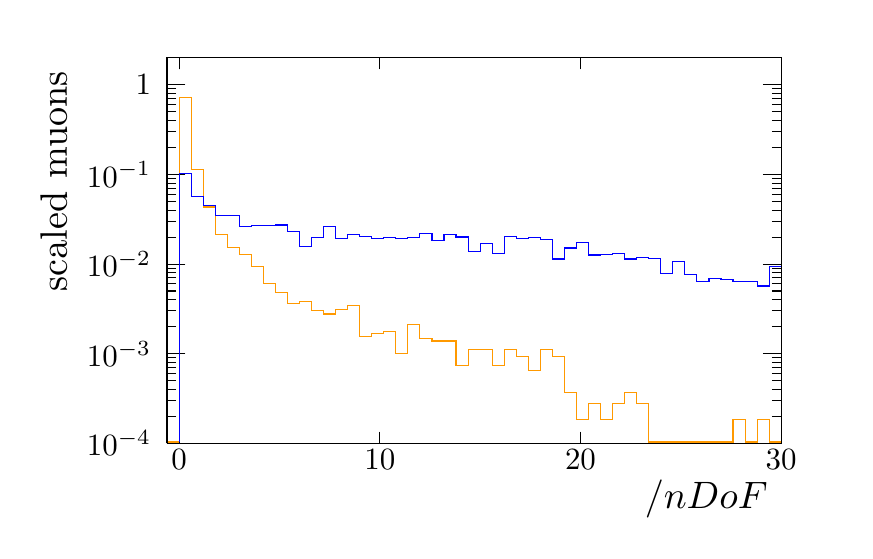
\begin{tikzpicture}
\pgfdeclareplotmark{cross} {
\pgfpathmoveto{\pgfpoint{-0.3\pgfplotmarksize}{\pgfplotmarksize}}
\pgfpathlineto{\pgfpoint{+0.3\pgfplotmarksize}{\pgfplotmarksize}}
\pgfpathlineto{\pgfpoint{+0.3\pgfplotmarksize}{0.3\pgfplotmarksize}}
\pgfpathlineto{\pgfpoint{+1\pgfplotmarksize}{0.3\pgfplotmarksize}}
\pgfpathlineto{\pgfpoint{+1\pgfplotmarksize}{-0.3\pgfplotmarksize}}
\pgfpathlineto{\pgfpoint{+0.3\pgfplotmarksize}{-0.3\pgfplotmarksize}}
\pgfpathlineto{\pgfpoint{+0.3\pgfplotmarksize}{-1.\pgfplotmarksize}}
\pgfpathlineto{\pgfpoint{-0.3\pgfplotmarksize}{-1.\pgfplotmarksize}}
\pgfpathlineto{\pgfpoint{-0.3\pgfplotmarksize}{-0.3\pgfplotmarksize}}
\pgfpathlineto{\pgfpoint{-1.\pgfplotmarksize}{-0.3\pgfplotmarksize}}
\pgfpathlineto{\pgfpoint{-1.\pgfplotmarksize}{0.3\pgfplotmarksize}}
\pgfpathlineto{\pgfpoint{-0.3\pgfplotmarksize}{0.3\pgfplotmarksize}}
\pgfpathclose
\pgfusepathqstroke
}
\pgfdeclareplotmark{cross*} {
\pgfpathmoveto{\pgfpoint{-0.3\pgfplotmarksize}{\pgfplotmarksize}}
\pgfpathlineto{\pgfpoint{+0.3\pgfplotmarksize}{\pgfplotmarksize}}
\pgfpathlineto{\pgfpoint{+0.3\pgfplotmarksize}{0.3\pgfplotmarksize}}
\pgfpathlineto{\pgfpoint{+1\pgfplotmarksize}{0.3\pgfplotmarksize}}
\pgfpathlineto{\pgfpoint{+1\pgfplotmarksize}{-0.3\pgfplotmarksize}}
\pgfpathlineto{\pgfpoint{+0.3\pgfplotmarksize}{-0.3\pgfplotmarksize}}
\pgfpathlineto{\pgfpoint{+0.3\pgfplotmarksize}{-1.\pgfplotmarksize}}
\pgfpathlineto{\pgfpoint{-0.3\pgfplotmarksize}{-1.\pgfplotmarksize}}
\pgfpathlineto{\pgfpoint{-0.3\pgfplotmarksize}{-0.3\pgfplotmarksize}}
\pgfpathlineto{\pgfpoint{-1.\pgfplotmarksize}{-0.3\pgfplotmarksize}}
\pgfpathlineto{\pgfpoint{-1.\pgfplotmarksize}{0.3\pgfplotmarksize}}
\pgfpathlineto{\pgfpoint{-0.3\pgfplotmarksize}{0.3\pgfplotmarksize}}
\pgfpathclose
\pgfusepathqfillstroke
}
\pgfdeclareplotmark{newstar} {
\pgfpathmoveto{\pgfqpoint{0pt}{\pgfplotmarksize}}
\pgfpathlineto{\pgfqpointpolar{44}{0.5\pgfplotmarksize}}
\pgfpathlineto{\pgfqpointpolar{18}{\pgfplotmarksize}}
\pgfpathlineto{\pgfqpointpolar{-20}{0.5\pgfplotmarksize}}
\pgfpathlineto{\pgfqpointpolar{-54}{\pgfplotmarksize}}
\pgfpathlineto{\pgfqpointpolar{-90}{0.5\pgfplotmarksize}}
\pgfpathlineto{\pgfqpointpolar{234}{\pgfplotmarksize}}
\pgfpathlineto{\pgfqpointpolar{198}{0.5\pgfplotmarksize}}
\pgfpathlineto{\pgfqpointpolar{162}{\pgfplotmarksize}}
\pgfpathlineto{\pgfqpointpolar{134}{0.5\pgfplotmarksize}}
\pgfpathclose
\pgfusepathqstroke
}
\pgfdeclareplotmark{newstar*} {
\pgfpathmoveto{\pgfqpoint{0pt}{\pgfplotmarksize}}
\pgfpathlineto{\pgfqpointpolar{44}{0.5\pgfplotmarksize}}
\pgfpathlineto{\pgfqpointpolar{18}{\pgfplotmarksize}}
\pgfpathlineto{\pgfqpointpolar{-20}{0.5\pgfplotmarksize}}
\pgfpathlineto{\pgfqpointpolar{-54}{\pgfplotmarksize}}
\pgfpathlineto{\pgfqpointpolar{-90}{0.5\pgfplotmarksize}}
\pgfpathlineto{\pgfqpointpolar{234}{\pgfplotmarksize}}
\pgfpathlineto{\pgfqpointpolar{198}{0.5\pgfplotmarksize}}
\pgfpathlineto{\pgfqpointpolar{162}{\pgfplotmarksize}}
\pgfpathlineto{\pgfqpointpolar{134}{0.5\pgfplotmarksize}}
\pgfpathclose
\pgfusepathqfillstroke
}
\definecolor{c}{rgb}{1,1,1};
\draw [color=c, fill=c] (0,0) rectangle (10,6.27517);
\draw [color=c, fill=c] (1.4,1.00403) rectangle (9.2,5.89866);
\definecolor{c}{rgb}{0,0,0};
\draw [c] (1.4,1.00403) -- (1.4,5.89866) -- (9.2,5.89866) -- (9.2,1.00403) -- (1.4,1.00403);
\definecolor{c}{rgb}{1,1,1};
\draw [color=c, fill=c] (1.4,1.00403) rectangle (9.2,5.89866);
\definecolor{c}{rgb}{0,0,0};
\draw [c] (1.4,1.00403) -- (1.4,5.89866) -- (9.2,5.89866) -- (9.2,1.00403) -- (1.4,1.00403);
\definecolor{c}{rgb}{1,0.6,0};
\draw [c,line width=0.4] (1.41678,1.02081) -- (1.41678,1.02081) -- (1.55294,1.02081) -- (1.55294,5.40058) -- (1.70588,5.40058) -- (1.70588,4.48106) -- (1.85882,4.48106) -- (1.85882,4.00454) -- (2.01176,4.00454) -- (2.01176,3.66091) --
 (2.16471,3.66091) -- (2.16471,3.49122) -- (2.31765,3.49122) -- (2.31765,3.39992) -- (2.47059,3.39992) -- (2.47059,3.24566) -- (2.62353,3.24566) -- (2.62353,3.02783) -- (2.77647,3.02783) -- (2.77647,2.91755) -- (2.92941,2.91755) -- (2.92941,2.77536)
 -- (3.08235,2.77536) -- (3.08235,2.80008) -- (3.23529,2.80008) -- (3.23529,2.6928) -- (3.38824,2.6928) -- (3.38824,2.64569) -- (3.54118,2.64569) -- (3.54118,2.70755) -- (3.69412,2.70755) -- (3.69412,2.74935) -- (3.84706,2.74935) -- (3.84706,2.36498)
 -- (4,2.36498) -- (4,2.39323) -- (4.15294,2.39323) -- (4.15294,2.41995) -- (4.30588,2.41995) -- (4.30588,2.14983) -- (4.45882,2.14983) -- (4.45882,2.51438) -- (4.61176,2.51438) -- (4.61176,2.33502) -- (4.76471,2.33502) -- (4.76471,2.30312) --
 (4.91765,2.30312) -- (4.91765,2.30312) -- (5.07059,2.30312) -- (5.07059,1.99244) -- (5.22353,1.99244) -- (5.22353,2.19283) -- (5.37647,2.19283) -- (5.37647,2.19283) -- (5.52941,2.19283) -- (5.52941,1.99244) -- (5.68235,1.99244) -- (5.68235,2.19283)
 -- (5.83529,2.19283) -- (5.83529,2.10272) -- (5.98824,2.10272) -- (5.98824,1.92644) -- (6.14118,1.92644) -- (6.14118,2.19283) -- (6.29412,2.19283) -- (6.29412,2.10272) -- (6.44706,2.10272) -- (6.44706,1.64986) -- (6.6,1.64986) -- (6.6,1.30729) --
 (6.75294,1.30729) -- (6.75294,1.50768) -- (6.90588,1.50768) -- (6.90588,1.30729) -- (7.05882,1.30729) -- (7.05882,1.50768) -- (7.21176,1.50768) -- (7.21176,1.64986) -- (7.36471,1.64986) -- (7.36471,1.50768) -- (7.51765,1.50768) -- (7.51765,1.02081)
 -- (7.67059,1.02081) -- (7.67059,1.02081) -- (7.82353,1.02081) -- (7.82353,1.02081) -- (7.97647,1.02081) -- (7.97647,1.02081) -- (8.12941,1.02081) -- (8.12941,1.02081) -- (8.28235,1.02081) -- (8.28235,1.02081) -- (8.43529,1.02081) --
 (8.43529,1.02081) -- (8.58823,1.02081) -- (8.58823,1.30729) -- (8.74118,1.30729) -- (8.74118,1.02081) -- (8.89412,1.02081) -- (8.89412,1.30729) -- (9.04706,1.30729) -- (9.04706,1.02081) -- (9.2,1.02081) -- (9.2,1.02081);
\definecolor{c}{rgb}{0,0,0};
\draw [c,line width=0.4] (1.4,1.00403) -- (9.2,1.00403);
\draw [anchor= east] (9.2,0.301208) node[scale=1.37879, rotate=0]{$\chisq/\text{nDoF}$};
\draw [c,line width=0.4] (1.55294,1.15087) -- (1.55294,1.00403);
\draw [c,line width=0.4] (4.10196,1.15087) -- (4.10196,1.00403);
\draw [c,line width=0.4] (6.65098,1.15087) -- (6.65098,1.00403);
\draw [c,line width=0.4] (9.2,1.15087) -- (9.2,1.00403);
\draw [c,line width=0.4] (1.55294,1.15087) -- (1.55294,1.00403);
\draw [anchor=base] (1.55294,0.665168) node[scale=1.11794, rotate=0]{0};
\draw [anchor=base] (4.10196,0.665168) node[scale=1.11794, rotate=0]{10};
\draw [anchor=base] (6.65098,0.665168) node[scale=1.11794, rotate=0]{20};
\draw [anchor=base] (9.2,0.665168) node[scale=1.11794, rotate=0]{30};
\draw [c,line width=0.4] (1.4,5.89866) -- (9.2,5.89866);
\draw [c,line width=0.4] (1.55294,5.75182) -- (1.55294,5.89866);
\draw [c,line width=0.4] (4.10196,5.75182) -- (4.10196,5.89866);
\draw [c,line width=0.4] (6.65098,5.75182) -- (6.65098,5.89866);
\draw [c,line width=0.4] (9.2,5.75182) -- (9.2,5.89866);
\draw [c,line width=0.4] (1.55294,5.75182) -- (1.55294,5.89866);
\draw [c,line width=0.4] (1.4,1.00403) -- (1.4,5.89866);
\draw [anchor= east] (-0.04,5.89866) node[scale=1.37879, rotate=90]{scaled muons};
\draw [c,line width=0.4] (1.634,1.00403) -- (1.4,1.00403);
\draw [anchor= east] (1.336,1.00403) node[scale=1.11794, rotate=0]{$10^{-4}$};
\draw [c,line width=0.4] (1.517,1.3466) -- (1.4,1.3466);
\draw [c,line width=0.4] (1.517,1.547) -- (1.4,1.547);
\draw [c,line width=0.4] (1.517,1.68918) -- (1.4,1.68918);
\draw [c,line width=0.4] (1.517,1.79947) -- (1.4,1.79947);
\draw [c,line width=0.4] (1.517,1.88957) -- (1.4,1.88957);
\draw [c,line width=0.4] (1.517,1.96576) -- (1.4,1.96576);
\draw [c,line width=0.4] (1.517,2.03176) -- (1.4,2.03176);
\draw [c,line width=0.4] (1.517,2.08997) -- (1.4,2.08997);
\draw [c,line width=0.4] (1.634,2.14204) -- (1.4,2.14204);
\draw [anchor= east] (1.336,2.14204) node[scale=1.11794, rotate=0]{$10^{-3}$};
\draw [c,line width=0.4] (1.517,2.48462) -- (1.4,2.48462);
\draw [c,line width=0.4] (1.517,2.68501) -- (1.4,2.68501);
\draw [c,line width=0.4] (1.517,2.82719) -- (1.4,2.82719);
\draw [c,line width=0.4] (1.517,2.93748) -- (1.4,2.93748);
\draw [c,line width=0.4] (1.517,3.02759) -- (1.4,3.02759);
\draw [c,line width=0.4] (1.517,3.10377) -- (1.4,3.10377);
\draw [c,line width=0.4] (1.517,3.16977) -- (1.4,3.16977);
\draw [c,line width=0.4] (1.517,3.22798) -- (1.4,3.22798);
\draw [c,line width=0.4] (1.634,3.28005) -- (1.4,3.28005);
\draw [anchor= east] (1.336,3.28005) node[scale=1.11794, rotate=0]{$10^{-2}$};
\draw [c,line width=0.4] (1.517,3.62263) -- (1.4,3.62263);
\draw [c,line width=0.4] (1.517,3.82303) -- (1.4,3.82303);
\draw [c,line width=0.4] (1.517,3.96521) -- (1.4,3.96521);
\draw [c,line width=0.4] (1.517,4.07549) -- (1.4,4.07549);
\draw [c,line width=0.4] (1.517,4.1656) -- (1.4,4.1656);
\draw [c,line width=0.4] (1.517,4.24179) -- (1.4,4.24179);
\draw [c,line width=0.4] (1.517,4.30778) -- (1.4,4.30778);
\draw [c,line width=0.4] (1.517,4.366) -- (1.4,4.366);
\draw [c,line width=0.4] (1.634,4.41807) -- (1.4,4.41807);
\draw [anchor= east] (1.336,4.41807) node[scale=1.11794, rotate=0]{$10^{-1}$};
\draw [c,line width=0.4] (1.517,4.76064) -- (1.4,4.76064);
\draw [c,line width=0.4] (1.517,4.96104) -- (1.4,4.96104);
\draw [c,line width=0.4] (1.517,5.10322) -- (1.4,5.10322);
\draw [c,line width=0.4] (1.517,5.21351) -- (1.4,5.21351);
\draw [c,line width=0.4] (1.517,5.30361) -- (1.4,5.30361);
\draw [c,line width=0.4] (1.517,5.3798) -- (1.4,5.3798);
\draw [c,line width=0.4] (1.517,5.4458) -- (1.4,5.4458);
\draw [c,line width=0.4] (1.517,5.50401) -- (1.4,5.50401);
\draw [c,line width=0.4] (1.634,5.55608) -- (1.4,5.55608);
\draw [anchor= east] (1.336,5.55608) node[scale=1.11794, rotate=0]{1};
\draw [c,line width=0.4] (1.517,5.89866) -- (1.4,5.89866);
\draw [c,line width=0.4] (9.2,1.00403) -- (9.2,5.89866);
\draw [c,line width=0.4] (8.966,1.00403) -- (9.2,1.00403);
\draw [c,line width=0.4] (9.083,1.3466) -- (9.2,1.3466);
\draw [c,line width=0.4] (9.083,1.547) -- (9.2,1.547);
\draw [c,line width=0.4] (9.083,1.68918) -- (9.2,1.68918);
\draw [c,line width=0.4] (9.083,1.79947) -- (9.2,1.79947);
\draw [c,line width=0.4] (9.083,1.88957) -- (9.2,1.88957);
\draw [c,line width=0.4] (9.083,1.96576) -- (9.2,1.96576);
\draw [c,line width=0.4] (9.083,2.03176) -- (9.2,2.03176);
\draw [c,line width=0.4] (9.083,2.08997) -- (9.2,2.08997);
\draw [c,line width=0.4] (8.966,2.14204) -- (9.2,2.14204);
\draw [c,line width=0.4] (9.083,2.48462) -- (9.2,2.48462);
\draw [c,line width=0.4] (9.083,2.68501) -- (9.2,2.68501);
\draw [c,line width=0.4] (9.083,2.82719) -- (9.2,2.82719);
\draw [c,line width=0.4] (9.083,2.93748) -- (9.2,2.93748);
\draw [c,line width=0.4] (9.083,3.02759) -- (9.2,3.02759);
\draw [c,line width=0.4] (9.083,3.10377) -- (9.2,3.10377);
\draw [c,line width=0.4] (9.083,3.16977) -- (9.2,3.16977);
\draw [c,line width=0.4] (9.083,3.22798) -- (9.2,3.22798);
\draw [c,line width=0.4] (8.966,3.28005) -- (9.2,3.28005);
\draw [c,line width=0.4] (9.083,3.62263) -- (9.2,3.62263);
\draw [c,line width=0.4] (9.083,3.82303) -- (9.2,3.82303);
\draw [c,line width=0.4] (9.083,3.96521) -- (9.2,3.96521);
\draw [c,line width=0.4] (9.083,4.07549) -- (9.2,4.07549);
\draw [c,line width=0.4] (9.083,4.1656) -- (9.2,4.1656);
\draw [c,line width=0.4] (9.083,4.24179) -- (9.2,4.24179);
\draw [c,line width=0.4] (9.083,4.30778) -- (9.2,4.30778);
\draw [c,line width=0.4] (9.083,4.366) -- (9.2,4.366);
\draw [c,line width=0.4] (8.966,4.41807) -- (9.2,4.41807);
\draw [c,line width=0.4] (9.083,4.76064) -- (9.2,4.76064);
\draw [c,line width=0.4] (9.083,4.96104) -- (9.2,4.96104);
\draw [c,line width=0.4] (9.083,5.10322) -- (9.2,5.10322);
\draw [c,line width=0.4] (9.083,5.21351) -- (9.2,5.21351);
\draw [c,line width=0.4] (9.083,5.30361) -- (9.2,5.30361);
\draw [c,line width=0.4] (9.083,5.3798) -- (9.2,5.3798);
\draw [c,line width=0.4] (9.083,5.4458) -- (9.2,5.4458);
\draw [c,line width=0.4] (9.083,5.50401) -- (9.2,5.50401);
\draw [c,line width=0.4] (8.966,5.55608) -- (9.2,5.55608);
\draw [c,line width=0.4] (9.083,5.89866) -- (9.2,5.89866);
\definecolor{c}{rgb}{0,0,1};
\draw [c,line width=0.4] (1.55294,1.02081) -- (1.55294,4.43052) -- (1.70588,4.43052) -- (1.70588,4.13786) -- (1.85882,4.13786) -- (1.85882,4.02433) -- (2.01176,4.02433) -- (2.01176,3.89112) -- (2.16471,3.89112) -- (2.16471,3.89112) --
 (2.31765,3.89112) -- (2.31765,3.75248) -- (2.47059,3.75248) -- (2.47059,3.7664) -- (2.62353,3.7664) -- (2.62353,3.77096) -- (2.77647,3.77096) -- (2.77647,3.77547) -- (2.92941,3.77547) -- (2.92941,3.69778) -- (3.08235,3.69778) -- (3.08235,3.50779) --
 (3.23529,3.50779) -- (3.23529,3.61808) -- (3.38824,3.61808) -- (3.38824,3.75248) -- (3.54118,3.75248) -- (3.54118,3.60557) -- (3.69412,3.60557) -- (3.69412,3.65954) -- (3.84706,3.65954) -- (3.84706,3.63028) -- (4,3.63028) -- (4,3.59919) --
 (4.15294,3.59919) -- (4.15294,3.61808) -- (4.30588,3.61808) -- (4.30588,3.59919) -- (4.45882,3.59919) -- (4.45882,3.61808) -- (4.61176,3.61808) -- (4.61176,3.67077) -- (4.76471,3.67077) -- (4.76471,3.57955) -- (4.91765,3.57955) -- (4.91765,3.65954)
 -- (5.07059,3.65954) -- (5.07059,3.62422) -- (5.22353,3.62422) -- (5.22353,3.4418) -- (5.37647,3.4418) -- (5.37647,3.53776) -- (5.52941,3.53776) -- (5.52941,3.41459) -- (5.68235,3.41459) -- (5.68235,3.63028) -- (5.83529,3.63028) -- (5.83529,3.60557)
 -- (5.98824,3.60557) -- (5.98824,3.61808) -- (6.14118,3.61808) -- (6.14118,3.59273) -- (6.29412,3.59273) -- (6.29412,3.34458) -- (6.44706,3.34458) -- (6.44706,3.48407) -- (6.6,3.48407) -- (6.6,3.55208) -- (6.75294,3.55208) -- (6.75294,3.39558) --
 (6.90588,3.39558) -- (6.90588,3.40517) -- (7.05882,3.40517) -- (7.05882,3.41459) -- (7.21176,3.41459) -- (7.21176,3.34458) -- (7.36471,3.34458) -- (7.36471,3.36561) -- (7.51765,3.36561) -- (7.51765,3.35521) -- (7.67059,3.35521) -- (7.67059,3.16522)
 -- (7.82353,3.16522) -- (7.82353,3.31125) -- (7.97647,3.31125) -- (7.97647,3.14953) -- (8.12941,3.14953) -- (8.12941,3.0626) -- (8.28235,3.0626) -- (8.28235,3.09922) -- (8.43529,3.09922) -- (8.43529,3.08125) -- (8.58823,3.08125) -- (8.58823,3.0626)
 -- (8.74118,3.0626) -- (8.74118,3.0626) -- (8.89412,3.0626) -- (8.89412,3.002) -- (9.04706,3.002) -- (9.04706,3.25015) -- (9.2,3.25015);
\end{tikzpicture}
}
    \caption{}
    \label{mvm_chi2}
  \end{subfigure}
  \caption{\chisq comparison between the old \mvm (top row) and the new \mvTTm (bottom row) algorithms.}
 \label{mvm_chi2_comp}
\end{figure}

\begin{figure}[h]
  \centering
  \begin{subfigure}{0.5\textwidth}
    \tikzsetnextfilename{mvTTm_wind_eff_total_x}
    \scalebox{.6}{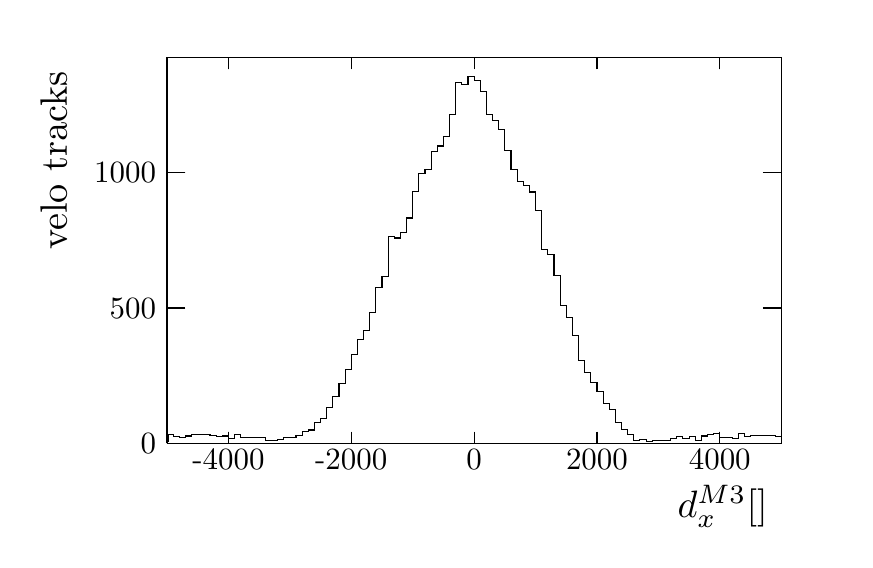
\begin{tikzpicture}
\pgfdeclareplotmark{cross} {
\pgfpathmoveto{\pgfpoint{-0.3\pgfplotmarksize}{\pgfplotmarksize}}
\pgfpathlineto{\pgfpoint{+0.3\pgfplotmarksize}{\pgfplotmarksize}}
\pgfpathlineto{\pgfpoint{+0.3\pgfplotmarksize}{0.3\pgfplotmarksize}}
\pgfpathlineto{\pgfpoint{+1\pgfplotmarksize}{0.3\pgfplotmarksize}}
\pgfpathlineto{\pgfpoint{+1\pgfplotmarksize}{-0.3\pgfplotmarksize}}
\pgfpathlineto{\pgfpoint{+0.3\pgfplotmarksize}{-0.3\pgfplotmarksize}}
\pgfpathlineto{\pgfpoint{+0.3\pgfplotmarksize}{-1.\pgfplotmarksize}}
\pgfpathlineto{\pgfpoint{-0.3\pgfplotmarksize}{-1.\pgfplotmarksize}}
\pgfpathlineto{\pgfpoint{-0.3\pgfplotmarksize}{-0.3\pgfplotmarksize}}
\pgfpathlineto{\pgfpoint{-1.\pgfplotmarksize}{-0.3\pgfplotmarksize}}
\pgfpathlineto{\pgfpoint{-1.\pgfplotmarksize}{0.3\pgfplotmarksize}}
\pgfpathlineto{\pgfpoint{-0.3\pgfplotmarksize}{0.3\pgfplotmarksize}}
\pgfpathclose
\pgfusepathqstroke
}
\pgfdeclareplotmark{cross*} {
\pgfpathmoveto{\pgfpoint{-0.3\pgfplotmarksize}{\pgfplotmarksize}}
\pgfpathlineto{\pgfpoint{+0.3\pgfplotmarksize}{\pgfplotmarksize}}
\pgfpathlineto{\pgfpoint{+0.3\pgfplotmarksize}{0.3\pgfplotmarksize}}
\pgfpathlineto{\pgfpoint{+1\pgfplotmarksize}{0.3\pgfplotmarksize}}
\pgfpathlineto{\pgfpoint{+1\pgfplotmarksize}{-0.3\pgfplotmarksize}}
\pgfpathlineto{\pgfpoint{+0.3\pgfplotmarksize}{-0.3\pgfplotmarksize}}
\pgfpathlineto{\pgfpoint{+0.3\pgfplotmarksize}{-1.\pgfplotmarksize}}
\pgfpathlineto{\pgfpoint{-0.3\pgfplotmarksize}{-1.\pgfplotmarksize}}
\pgfpathlineto{\pgfpoint{-0.3\pgfplotmarksize}{-0.3\pgfplotmarksize}}
\pgfpathlineto{\pgfpoint{-1.\pgfplotmarksize}{-0.3\pgfplotmarksize}}
\pgfpathlineto{\pgfpoint{-1.\pgfplotmarksize}{0.3\pgfplotmarksize}}
\pgfpathlineto{\pgfpoint{-0.3\pgfplotmarksize}{0.3\pgfplotmarksize}}
\pgfpathclose
\pgfusepathqfillstroke
}
\pgfdeclareplotmark{newstar} {
\pgfpathmoveto{\pgfqpoint{0pt}{\pgfplotmarksize}}
\pgfpathlineto{\pgfqpointpolar{44}{0.5\pgfplotmarksize}}
\pgfpathlineto{\pgfqpointpolar{18}{\pgfplotmarksize}}
\pgfpathlineto{\pgfqpointpolar{-20}{0.5\pgfplotmarksize}}
\pgfpathlineto{\pgfqpointpolar{-54}{\pgfplotmarksize}}
\pgfpathlineto{\pgfqpointpolar{-90}{0.5\pgfplotmarksize}}
\pgfpathlineto{\pgfqpointpolar{234}{\pgfplotmarksize}}
\pgfpathlineto{\pgfqpointpolar{198}{0.5\pgfplotmarksize}}
\pgfpathlineto{\pgfqpointpolar{162}{\pgfplotmarksize}}
\pgfpathlineto{\pgfqpointpolar{134}{0.5\pgfplotmarksize}}
\pgfpathclose
\pgfusepathqstroke
}
\pgfdeclareplotmark{newstar*} {
\pgfpathmoveto{\pgfqpoint{0pt}{\pgfplotmarksize}}
\pgfpathlineto{\pgfqpointpolar{44}{0.5\pgfplotmarksize}}
\pgfpathlineto{\pgfqpointpolar{18}{\pgfplotmarksize}}
\pgfpathlineto{\pgfqpointpolar{-20}{0.5\pgfplotmarksize}}
\pgfpathlineto{\pgfqpointpolar{-54}{\pgfplotmarksize}}
\pgfpathlineto{\pgfqpointpolar{-90}{0.5\pgfplotmarksize}}
\pgfpathlineto{\pgfqpointpolar{234}{\pgfplotmarksize}}
\pgfpathlineto{\pgfqpointpolar{198}{0.5\pgfplotmarksize}}
\pgfpathlineto{\pgfqpointpolar{162}{\pgfplotmarksize}}
\pgfpathlineto{\pgfqpointpolar{134}{0.5\pgfplotmarksize}}
\pgfpathclose
\pgfusepathqfillstroke
}
\definecolor{c}{rgb}{1,1,1};
\draw [color=c, fill=c] (0,0) rectangle (10,6.27517);
\draw [color=c, fill=c] (1.4,1.00403) rectangle (9.2,5.89866);
\definecolor{c}{rgb}{0,0,0};
\draw [c] (1.4,1.00403) -- (1.4,5.89866) -- (9.2,5.89866) -- (9.2,1.00403) -- (1.4,1.00403);
\definecolor{c}{rgb}{1,1,1};
\draw [color=c, fill=c] (1.4,1.00403) rectangle (9.2,5.89866);
\definecolor{c}{rgb}{0,0,0};
\draw [c] (1.4,1.00403) -- (1.4,5.89866) -- (9.2,5.89866) -- (9.2,1.00403) -- (1.4,1.00403);
\draw [c,line width=0.4] (1.41678,1.02081) -- (1.41678,1.12082) -- (1.478,1.12082) -- (1.478,1.08647) -- (1.556,1.08647) -- (1.556,1.07617) -- (1.634,1.07617) -- (1.634,1.09678) -- (1.712,1.09678) -- (1.712,1.11395) -- (1.79,1.11395) --
 (1.79,1.11739) -- (1.868,1.11739) -- (1.868,1.11395) -- (1.946,1.11395) -- (1.946,1.10708) -- (2.024,1.10708) -- (2.024,1.09334) -- (2.102,1.09334) -- (2.102,1.09678) -- (2.18,1.09678) -- (2.18,1.0693) -- (2.258,1.0693) -- (2.258,1.11052) --
 (2.336,1.11052) -- (2.336,1.07273) -- (2.414,1.07273) -- (2.414,1.08304) -- (2.492,1.08304) -- (2.492,1.07617) -- (2.57,1.07617) -- (2.57,1.07273) -- (2.648,1.07273) -- (2.648,1.03838) -- (2.726,1.03838) -- (2.726,1.03494) -- (2.804,1.03494) --
 (2.804,1.04868) -- (2.882,1.04868) -- (2.882,1.08304) -- (2.96,1.08304) -- (2.96,1.07617) -- (3.038,1.07617) -- (3.038,1.10708) -- (3.116,1.10708) -- (3.116,1.1483) -- (3.194,1.1483) -- (3.194,1.17235) -- (3.272,1.17235) -- (3.272,1.27197) --
 (3.35,1.27197) -- (3.35,1.31663) -- (3.428,1.31663) -- (3.428,1.45404) -- (3.506,1.45404) -- (3.506,1.59831) -- (3.584,1.59831) -- (3.584,1.76664) -- (3.662,1.76664) -- (3.662,1.94183) -- (3.74,1.94183) -- (3.74,2.1342) -- (3.818,2.1342) --
 (3.818,2.32314) -- (3.896,2.32314) -- (3.896,2.43307) -- (3.974,2.43307) -- (3.974,2.67009) -- (4.052,2.67009) -- (4.052,2.9827) -- (4.13,2.9827) -- (4.13,3.11667) -- (4.208,3.11667) -- (4.208,3.63195) -- (4.286,3.63195) -- (4.286,3.61134) --
 (4.364,3.61134) -- (4.364,3.6766) -- (4.442,3.6766) -- (4.442,3.86554) -- (4.52,3.86554) -- (4.52,4.20562) -- (4.598,4.20562) -- (4.598,4.42891) -- (4.676,4.42891) -- (4.676,4.477) -- (4.754,4.477) -- (4.754,4.7106) -- (4.832,4.7106) --
 (4.832,4.7793) -- (4.91,4.7793) -- (4.91,4.8961) -- (4.988,4.8961) -- (4.988,5.18465) -- (5.066,5.18465) -- (5.066,5.58314) -- (5.144,5.58314) -- (5.144,5.55565) -- (5.222,5.55565) -- (5.222,5.66558) -- (5.3,5.66558) -- (5.3,5.60718) --
 (5.378,5.60718) -- (5.378,5.46977) -- (5.456,5.46977) -- (5.456,5.18465) -- (5.534,5.18465) -- (5.534,5.10221) -- (5.612,5.10221) -- (5.612,4.99228) -- (5.69,4.99228) -- (5.69,4.72777) -- (5.768,4.72777) -- (5.768,4.477) -- (5.846,4.477) --
 (5.846,4.32929) -- (5.924,4.32929) -- (5.924,4.27776) -- (6.002,4.27776) -- (6.002,4.19532) -- (6.08,4.19532) -- (6.08,3.96173) -- (6.158,3.96173) -- (6.158,3.46706) -- (6.236,3.46706) -- (6.236,3.40179) -- (6.314,3.40179) -- (6.314,3.13041) --
 (6.392,3.13041) -- (6.392,2.75254) -- (6.47,2.75254) -- (6.47,2.60139) -- (6.548,2.60139) -- (6.548,2.3781) -- (6.626,2.3781) -- (6.626,2.05176) -- (6.704,2.05176) -- (6.704,1.90405) -- (6.782,1.90405) -- (6.782,1.77351) -- (6.86,1.77351) --
 (6.86,1.66358) -- (6.938,1.66358) -- (6.938,1.50556) -- (7.016,1.50556) -- (7.016,1.43686) -- (7.094,1.43686) -- (7.094,1.27197) -- (7.172,1.27197) -- (7.172,1.18266) -- (7.25,1.18266) -- (7.25,1.11395) -- (7.328,1.11395) -- (7.328,1.03838) --
 (7.406,1.03838) -- (7.406,1.04868) -- (7.484,1.04868) -- (7.484,1.0212) -- (7.562,1.0212) -- (7.562,1.04181) -- (7.64,1.04181) -- (7.64,1.03494) -- (7.718,1.03494) -- (7.718,1.03838) -- (7.796,1.03838) -- (7.796,1.06243) -- (7.874,1.06243) --
 (7.874,1.08647) -- (7.952,1.08647) -- (7.952,1.0693) -- (8.03,1.0693) -- (8.03,1.08647) -- (8.108,1.08647) -- (8.108,1.03494) -- (8.186,1.03494) -- (8.186,1.09678) -- (8.264,1.09678) -- (8.264,1.11395) -- (8.342,1.11395) -- (8.342,1.12769) --
 (8.42,1.12769) -- (8.42,1.08304) -- (8.498,1.08304) -- (8.498,1.07273) -- (8.576,1.07273) -- (8.576,1.06586) -- (8.654,1.06586) -- (8.654,1.12769) -- (8.732,1.12769) -- (8.732,1.08991) -- (8.81,1.08991) -- (8.81,1.10365) -- (8.888,1.10365) --
 (8.888,1.10365) -- (8.966,1.10365) -- (8.966,1.10021) -- (9.044,1.10021) -- (9.044,1.10365) -- (9.122,1.10365) -- (9.122,1.09334) -- (9.2,1.09334);
\draw [c,line width=0.4] (1.4,1.00403) -- (9.2,1.00403);
\draw [anchor= east] (9.2,0.200805) node[scale=1.37879, rotate=0]{$d^{\text{M3}}_x [\mm]$};
\draw [c,line width=0.4] (2.18,1.15087) -- (2.18,1.00403);
\draw [c,line width=0.4] (3.74,1.15087) -- (3.74,1.00403);
\draw [c,line width=0.4] (5.3,1.15087) -- (5.3,1.00403);
\draw [c,line width=0.4] (6.86,1.15087) -- (6.86,1.00403);
\draw [c,line width=0.4] (8.42,1.15087) -- (8.42,1.00403);
\draw [c,line width=0.4] (2.18,1.15087) -- (2.18,1.00403);
\draw [c,line width=0.4] (8.42,1.15087) -- (8.42,1.00403);
\draw [anchor=base] (2.18,0.665168) node[scale=1.11794, rotate=0]{-4000};
\draw [anchor=base] (3.74,0.665168) node[scale=1.11794, rotate=0]{-2000};
\draw [anchor=base] (5.3,0.665168) node[scale=1.11794, rotate=0]{0};
\draw [anchor=base] (6.86,0.665168) node[scale=1.11794, rotate=0]{2000};
\draw [anchor=base] (8.42,0.665168) node[scale=1.11794, rotate=0]{4000};
\draw [c,line width=0.4] (1.4,5.89866) -- (9.2,5.89866);
\draw [c,line width=0.4] (2.18,5.75182) -- (2.18,5.89866);
\draw [c,line width=0.4] (3.74,5.75182) -- (3.74,5.89866);
\draw [c,line width=0.4] (5.3,5.75182) -- (5.3,5.89866);
\draw [c,line width=0.4] (6.86,5.75182) -- (6.86,5.89866);
\draw [c,line width=0.4] (8.42,5.75182) -- (8.42,5.89866);
\draw [c,line width=0.4] (2.18,5.75182) -- (2.18,5.89866);
\draw [c,line width=0.4] (8.42,5.75182) -- (8.42,5.89866);
\draw [c,line width=0.4] (1.4,1.00403) -- (1.4,5.89866);
\draw [anchor= east] (-0.04,5.89866) node[scale=1.37879, rotate=90]{velo tracks};
\draw [c,line width=0.4] (1.634,1.00403) -- (1.4,1.00403);
\draw [c,line width=0.4] (1.634,2.72162) -- (1.4,2.72162);
\draw [c,line width=0.4] (1.634,4.43922) -- (1.4,4.43922);
\draw [c,line width=0.4] (1.634,4.43922) -- (1.4,4.43922);
\draw [anchor= east] (1.4,1.00403) node[scale=1.11794, rotate=0]{0};
\draw [anchor= east] (1.4,2.72162) node[scale=1.11794, rotate=0]{500};
\draw [anchor= east] (1.4,4.43922) node[scale=1.11794, rotate=0]{1000};
\draw [c,line width=0.4] (9.2,1.00403) -- (9.2,5.89866);
\draw [c,line width=0.4] (8.966,1.00403) -- (9.2,1.00403);
\draw [c,line width=0.4] (8.966,2.72162) -- (9.2,2.72162);
\draw [c,line width=0.4] (8.966,4.43922) -- (9.2,4.43922);
\draw [c,line width=0.4] (8.966,4.43922) -- (9.2,4.43922);
\end{tikzpicture}
}
    \caption{}
    \label{mvTTm_res_x}
  \end{subfigure}%
  \hfill%
  \begin{subfigure}{0.5\textwidth}
    \tikzsetnextfilename{mvTTm_wind_eff_total_y}
    \scalebox{.6}{\begin{tikzpicture}
\pgfdeclareplotmark{cross} {
\pgfpathmoveto{\pgfpoint{-0.3\pgfplotmarksize}{\pgfplotmarksize}}
\pgfpathlineto{\pgfpoint{+0.3\pgfplotmarksize}{\pgfplotmarksize}}
\pgfpathlineto{\pgfpoint{+0.3\pgfplotmarksize}{0.3\pgfplotmarksize}}
\pgfpathlineto{\pgfpoint{+1\pgfplotmarksize}{0.3\pgfplotmarksize}}
\pgfpathlineto{\pgfpoint{+1\pgfplotmarksize}{-0.3\pgfplotmarksize}}
\pgfpathlineto{\pgfpoint{+0.3\pgfplotmarksize}{-0.3\pgfplotmarksize}}
\pgfpathlineto{\pgfpoint{+0.3\pgfplotmarksize}{-1.\pgfplotmarksize}}
\pgfpathlineto{\pgfpoint{-0.3\pgfplotmarksize}{-1.\pgfplotmarksize}}
\pgfpathlineto{\pgfpoint{-0.3\pgfplotmarksize}{-0.3\pgfplotmarksize}}
\pgfpathlineto{\pgfpoint{-1.\pgfplotmarksize}{-0.3\pgfplotmarksize}}
\pgfpathlineto{\pgfpoint{-1.\pgfplotmarksize}{0.3\pgfplotmarksize}}
\pgfpathlineto{\pgfpoint{-0.3\pgfplotmarksize}{0.3\pgfplotmarksize}}
\pgfpathclose
\pgfusepathqstroke
}
\pgfdeclareplotmark{cross*} {
\pgfpathmoveto{\pgfpoint{-0.3\pgfplotmarksize}{\pgfplotmarksize}}
\pgfpathlineto{\pgfpoint{+0.3\pgfplotmarksize}{\pgfplotmarksize}}
\pgfpathlineto{\pgfpoint{+0.3\pgfplotmarksize}{0.3\pgfplotmarksize}}
\pgfpathlineto{\pgfpoint{+1\pgfplotmarksize}{0.3\pgfplotmarksize}}
\pgfpathlineto{\pgfpoint{+1\pgfplotmarksize}{-0.3\pgfplotmarksize}}
\pgfpathlineto{\pgfpoint{+0.3\pgfplotmarksize}{-0.3\pgfplotmarksize}}
\pgfpathlineto{\pgfpoint{+0.3\pgfplotmarksize}{-1.\pgfplotmarksize}}
\pgfpathlineto{\pgfpoint{-0.3\pgfplotmarksize}{-1.\pgfplotmarksize}}
\pgfpathlineto{\pgfpoint{-0.3\pgfplotmarksize}{-0.3\pgfplotmarksize}}
\pgfpathlineto{\pgfpoint{-1.\pgfplotmarksize}{-0.3\pgfplotmarksize}}
\pgfpathlineto{\pgfpoint{-1.\pgfplotmarksize}{0.3\pgfplotmarksize}}
\pgfpathlineto{\pgfpoint{-0.3\pgfplotmarksize}{0.3\pgfplotmarksize}}
\pgfpathclose
\pgfusepathqfillstroke
}
\pgfdeclareplotmark{newstar} {
\pgfpathmoveto{\pgfqpoint{0pt}{\pgfplotmarksize}}
\pgfpathlineto{\pgfqpointpolar{44}{0.5\pgfplotmarksize}}
\pgfpathlineto{\pgfqpointpolar{18}{\pgfplotmarksize}}
\pgfpathlineto{\pgfqpointpolar{-20}{0.5\pgfplotmarksize}}
\pgfpathlineto{\pgfqpointpolar{-54}{\pgfplotmarksize}}
\pgfpathlineto{\pgfqpointpolar{-90}{0.5\pgfplotmarksize}}
\pgfpathlineto{\pgfqpointpolar{234}{\pgfplotmarksize}}
\pgfpathlineto{\pgfqpointpolar{198}{0.5\pgfplotmarksize}}
\pgfpathlineto{\pgfqpointpolar{162}{\pgfplotmarksize}}
\pgfpathlineto{\pgfqpointpolar{134}{0.5\pgfplotmarksize}}
\pgfpathclose
\pgfusepathqstroke
}
\pgfdeclareplotmark{newstar*} {
\pgfpathmoveto{\pgfqpoint{0pt}{\pgfplotmarksize}}
\pgfpathlineto{\pgfqpointpolar{44}{0.5\pgfplotmarksize}}
\pgfpathlineto{\pgfqpointpolar{18}{\pgfplotmarksize}}
\pgfpathlineto{\pgfqpointpolar{-20}{0.5\pgfplotmarksize}}
\pgfpathlineto{\pgfqpointpolar{-54}{\pgfplotmarksize}}
\pgfpathlineto{\pgfqpointpolar{-90}{0.5\pgfplotmarksize}}
\pgfpathlineto{\pgfqpointpolar{234}{\pgfplotmarksize}}
\pgfpathlineto{\pgfqpointpolar{198}{0.5\pgfplotmarksize}}
\pgfpathlineto{\pgfqpointpolar{162}{\pgfplotmarksize}}
\pgfpathlineto{\pgfqpointpolar{134}{0.5\pgfplotmarksize}}
\pgfpathclose
\pgfusepathqfillstroke
}
\definecolor{c}{rgb}{1,1,1};
\draw [color=c, fill=c] (0,0) rectangle (10,6.27517);
\draw [color=c, fill=c] (1.4,1.00403) rectangle (9.2,5.89866);
\definecolor{c}{rgb}{0,0,0};
\draw [c] (1.4,1.00403) -- (1.4,5.89866) -- (9.2,5.89866) -- (9.2,1.00403) -- (1.4,1.00403);
\definecolor{c}{rgb}{1,1,1};
\draw [color=c, fill=c] (1.4,1.00403) rectangle (9.2,5.89866);
\definecolor{c}{rgb}{0,0,0};
\draw [c] (1.4,1.00403) -- (1.4,5.89866) -- (9.2,5.89866) -- (9.2,1.00403) -- (1.4,1.00403);
\draw [c,line width=0.4] (1.41678,1.02081) -- (1.41678,1.02081) -- (1.478,1.02081) -- (1.478,1.02081) -- (1.556,1.02081) -- (1.556,1.02081) -- (1.634,1.02081) -- (1.634,1.02081) -- (1.712,1.02081) -- (1.712,1.02081) -- (1.79,1.02081) --
 (1.79,1.02081) -- (1.868,1.02081) -- (1.868,1.02081) -- (1.946,1.02081) -- (1.946,1.02081) -- (2.024,1.02081) -- (2.024,1.02081) -- (2.102,1.02081) -- (2.102,1.02081) -- (2.18,1.02081) -- (2.18,1.02081) -- (2.258,1.02081) -- (2.258,1.02081) --
 (2.336,1.02081) -- (2.336,1.02081) -- (2.414,1.02081) -- (2.414,1.02081) -- (2.492,1.02081) -- (2.492,1.02081) -- (2.57,1.02081) -- (2.57,1.02081) -- (2.648,1.02081) -- (2.648,1.02081) -- (2.726,1.02081) -- (2.726,1.02081) -- (2.804,1.02081) --
 (2.804,1.02081) -- (2.882,1.02081) -- (2.882,1.02081) -- (2.96,1.02081) -- (2.96,1.02081) -- (3.038,1.02081) -- (3.038,1.02081) -- (3.116,1.02081) -- (3.116,1.02081) -- (3.194,1.02081) -- (3.194,1.02081) -- (3.272,1.02081) -- (3.272,1.02081) --
 (3.35,1.02081) -- (3.35,1.02081) -- (3.428,1.02081) -- (3.428,1.02081) -- (3.506,1.02081) -- (3.506,1.02081) -- (3.584,1.02081) -- (3.584,1.02081) -- (3.662,1.02081) -- (3.662,1.02081) -- (3.74,1.02081) -- (3.74,1.02081) -- (3.818,1.02081) --
 (3.818,1.02081) -- (3.896,1.02081) -- (3.896,1.02081) -- (3.974,1.02081) -- (3.974,1.02081) -- (4.052,1.02081) -- (4.052,1.02081) -- (4.13,1.02081) -- (4.13,1.02081) -- (4.208,1.02081) -- (4.208,1.02081) -- (4.286,1.02081) -- (4.286,1.02081) --
 (4.364,1.02081) -- (4.364,1.02081) -- (4.442,1.02081) -- (4.442,1.02081) -- (4.52,1.02081) -- (4.52,1.02081) -- (4.598,1.02081) -- (4.598,1.02081) -- (4.676,1.02081) -- (4.676,1.02114) -- (4.754,1.02114) -- (4.754,1.0394) -- (4.832,1.0394) --
 (4.832,1.06184) -- (4.91,1.06184) -- (4.91,1.10405) -- (4.988,1.10405) -- (4.988,1.22727) -- (5.066,1.22727) -- (5.066,1.55625) -- (5.144,1.55625) -- (5.144,2.62646) -- (5.222,2.62646) -- (5.222,5.66558) -- (5.3,5.66558) -- (5.3,5.5165) --
 (5.378,5.5165) -- (5.378,2.4268) -- (5.456,2.4268) -- (5.456,1.54484) -- (5.534,1.54484) -- (5.534,1.21739) -- (5.612,1.21739) -- (5.612,1.08922) -- (5.69,1.08922) -- (5.69,1.03521) -- (5.768,1.03521) -- (5.768,1.02081) -- (5.846,1.02081) --
 (5.846,1.02081) -- (5.924,1.02081) -- (5.924,1.02081) -- (6.002,1.02081) -- (6.002,1.02081) -- (6.08,1.02081) -- (6.08,1.02081) -- (6.158,1.02081) -- (6.158,1.02081) -- (6.236,1.02081) -- (6.236,1.02081) -- (6.314,1.02081) -- (6.314,1.02081) --
 (6.392,1.02081) -- (6.392,1.02081) -- (6.47,1.02081) -- (6.47,1.02081) -- (6.548,1.02081) -- (6.548,1.02081) -- (6.626,1.02081) -- (6.626,1.02081) -- (6.704,1.02081) -- (6.704,1.02081) -- (6.782,1.02081) -- (6.782,1.02081) -- (6.86,1.02081) --
 (6.86,1.02081) -- (6.938,1.02081) -- (6.938,1.02081) -- (7.016,1.02081) -- (7.016,1.02081) -- (7.094,1.02081) -- (7.094,1.02081) -- (7.172,1.02081) -- (7.172,1.02081) -- (7.25,1.02081) -- (7.25,1.02081) -- (7.328,1.02081) -- (7.328,1.02081) --
 (7.406,1.02081) -- (7.406,1.02081) -- (7.484,1.02081) -- (7.484,1.02081) -- (7.562,1.02081) -- (7.562,1.02081) -- (7.64,1.02081) -- (7.64,1.02081) -- (7.718,1.02081) -- (7.718,1.02081) -- (7.796,1.02081) -- (7.796,1.02081) -- (7.874,1.02081) --
 (7.874,1.02081) -- (7.952,1.02081) -- (7.952,1.02081) -- (8.03,1.02081) -- (8.03,1.02081) -- (8.108,1.02081) -- (8.108,1.02081) -- (8.186,1.02081) -- (8.186,1.02081) -- (8.264,1.02081) -- (8.264,1.02081) -- (8.342,1.02081) -- (8.342,1.02081) --
 (8.42,1.02081) -- (8.42,1.02081) -- (8.498,1.02081) -- (8.498,1.02081) -- (8.576,1.02081) -- (8.576,1.02081) -- (8.654,1.02081) -- (8.654,1.02081) -- (8.732,1.02081) -- (8.732,1.02081) -- (8.81,1.02081) -- (8.81,1.02081) -- (8.888,1.02081) --
 (8.888,1.02081) -- (8.966,1.02081) -- (8.966,1.02081) -- (9.044,1.02081) -- (9.044,1.02081) -- (9.122,1.02081) -- (9.122,1.02081) -- (9.2,1.02081);
\draw [c,line width=0.4] (1.4,1.00403) -- (9.2,1.00403);
\draw [anchor= east] (9.2,0.200805) node[scale=1.37879, rotate=0]{$d^{\text{M3}}_y [\mm]$};
\draw [c,line width=0.4] (2.18,1.15087) -- (2.18,1.00403);
\draw [c,line width=0.4] (3.74,1.15087) -- (3.74,1.00403);
\draw [c,line width=0.4] (5.3,1.15087) -- (5.3,1.00403);
\draw [c,line width=0.4] (6.86,1.15087) -- (6.86,1.00403);
\draw [c,line width=0.4] (8.42,1.15087) -- (8.42,1.00403);
\draw [c,line width=0.4] (2.18,1.15087) -- (2.18,1.00403);
\draw [c,line width=0.4] (8.42,1.15087) -- (8.42,1.00403);
\draw [anchor=base] (2.18,0.665168) node[scale=1.11794, rotate=0]{-4000};
\draw [anchor=base] (3.74,0.665168) node[scale=1.11794, rotate=0]{-2000};
\draw [anchor=base] (5.3,0.665168) node[scale=1.11794, rotate=0]{0};
\draw [anchor=base] (6.86,0.665168) node[scale=1.11794, rotate=0]{2000};
\draw [anchor=base] (8.42,0.665168) node[scale=1.11794, rotate=0]{4000};
\draw [c,line width=0.4] (1.4,5.89866) -- (9.2,5.89866);
\draw [c,line width=0.4] (2.18,5.75182) -- (2.18,5.89866);
\draw [c,line width=0.4] (3.74,5.75182) -- (3.74,5.89866);
\draw [c,line width=0.4] (5.3,5.75182) -- (5.3,5.89866);
\draw [c,line width=0.4] (6.86,5.75182) -- (6.86,5.89866);
\draw [c,line width=0.4] (8.42,5.75182) -- (8.42,5.89866);
\draw [c,line width=0.4] (2.18,5.75182) -- (2.18,5.89866);
\draw [c,line width=0.4] (8.42,5.75182) -- (8.42,5.89866);
\draw [c,line width=0.4] (1.4,1.00403) -- (1.4,5.89866);
\draw [anchor= east] (-0.04,5.89866) node[scale=1.37879, rotate=90]{velo tracks};
\draw [c,line width=0.4] (1.634,1.00403) -- (1.4,1.00403);
\draw [c,line width=0.4] (1.634,2.90562) -- (1.4,2.90562);
\draw [c,line width=0.4] (1.634,4.8072) -- (1.4,4.8072);
\draw [c,line width=0.4] (1.634,4.8072) -- (1.4,4.8072);
\draw [anchor= east] (1.4,1.00403) node[scale=1.11794, rotate=0]{0};
\draw [anchor= east] (1.4,2.90562) node[scale=1.11794, rotate=0]{5};
\draw [anchor= east] (1.4,4.8072) node[scale=1.11794, rotate=0]{10};
\draw [anchor=base west] (1.4,5.94886) node[scale=1.11794, rotate=0]{$\times10^{3}$};
\draw [c,line width=0.4] (9.2,1.00403) -- (9.2,5.89866);
\draw [c,line width=0.4] (8.966,1.00403) -- (9.2,1.00403);
\draw [c,line width=0.4] (8.966,2.90562) -- (9.2,2.90562);
\draw [c,line width=0.4] (8.966,4.8072) -- (9.2,4.8072);
\draw [c,line width=0.4] (8.966,4.8072) -- (9.2,4.8072);
\end{tikzpicture}
}
    \caption{}
    \label{mvm_res_y}
  \end{subfigure}
  \caption{Residulas.  }
 \label{mvm_res}
\end{figure}

\begin{figure}[h]
  \centering
  \begin{subfigure}{0.5\textwidth}
    \tikzsetnextfilename{mvTTm_wind_eff_pos_neg_dx_norm}
    \scalebox{.6}{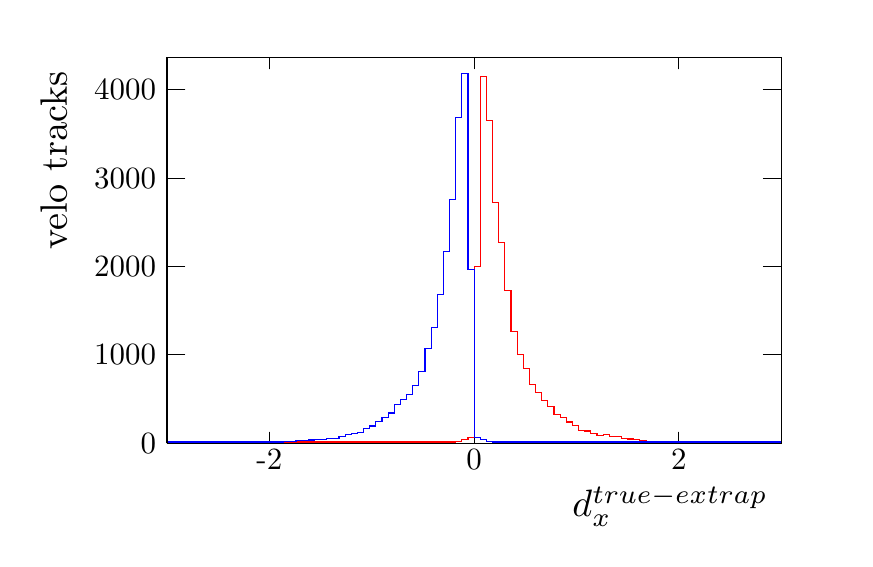
\begin{tikzpicture}
\pgfdeclareplotmark{cross} {
\pgfpathmoveto{\pgfpoint{-0.3\pgfplotmarksize}{\pgfplotmarksize}}
\pgfpathlineto{\pgfpoint{+0.3\pgfplotmarksize}{\pgfplotmarksize}}
\pgfpathlineto{\pgfpoint{+0.3\pgfplotmarksize}{0.3\pgfplotmarksize}}
\pgfpathlineto{\pgfpoint{+1\pgfplotmarksize}{0.3\pgfplotmarksize}}
\pgfpathlineto{\pgfpoint{+1\pgfplotmarksize}{-0.3\pgfplotmarksize}}
\pgfpathlineto{\pgfpoint{+0.3\pgfplotmarksize}{-0.3\pgfplotmarksize}}
\pgfpathlineto{\pgfpoint{+0.3\pgfplotmarksize}{-1.\pgfplotmarksize}}
\pgfpathlineto{\pgfpoint{-0.3\pgfplotmarksize}{-1.\pgfplotmarksize}}
\pgfpathlineto{\pgfpoint{-0.3\pgfplotmarksize}{-0.3\pgfplotmarksize}}
\pgfpathlineto{\pgfpoint{-1.\pgfplotmarksize}{-0.3\pgfplotmarksize}}
\pgfpathlineto{\pgfpoint{-1.\pgfplotmarksize}{0.3\pgfplotmarksize}}
\pgfpathlineto{\pgfpoint{-0.3\pgfplotmarksize}{0.3\pgfplotmarksize}}
\pgfpathclose
\pgfusepathqstroke
}
\pgfdeclareplotmark{cross*} {
\pgfpathmoveto{\pgfpoint{-0.3\pgfplotmarksize}{\pgfplotmarksize}}
\pgfpathlineto{\pgfpoint{+0.3\pgfplotmarksize}{\pgfplotmarksize}}
\pgfpathlineto{\pgfpoint{+0.3\pgfplotmarksize}{0.3\pgfplotmarksize}}
\pgfpathlineto{\pgfpoint{+1\pgfplotmarksize}{0.3\pgfplotmarksize}}
\pgfpathlineto{\pgfpoint{+1\pgfplotmarksize}{-0.3\pgfplotmarksize}}
\pgfpathlineto{\pgfpoint{+0.3\pgfplotmarksize}{-0.3\pgfplotmarksize}}
\pgfpathlineto{\pgfpoint{+0.3\pgfplotmarksize}{-1.\pgfplotmarksize}}
\pgfpathlineto{\pgfpoint{-0.3\pgfplotmarksize}{-1.\pgfplotmarksize}}
\pgfpathlineto{\pgfpoint{-0.3\pgfplotmarksize}{-0.3\pgfplotmarksize}}
\pgfpathlineto{\pgfpoint{-1.\pgfplotmarksize}{-0.3\pgfplotmarksize}}
\pgfpathlineto{\pgfpoint{-1.\pgfplotmarksize}{0.3\pgfplotmarksize}}
\pgfpathlineto{\pgfpoint{-0.3\pgfplotmarksize}{0.3\pgfplotmarksize}}
\pgfpathclose
\pgfusepathqfillstroke
}
\pgfdeclareplotmark{newstar} {
\pgfpathmoveto{\pgfqpoint{0pt}{\pgfplotmarksize}}
\pgfpathlineto{\pgfqpointpolar{44}{0.5\pgfplotmarksize}}
\pgfpathlineto{\pgfqpointpolar{18}{\pgfplotmarksize}}
\pgfpathlineto{\pgfqpointpolar{-20}{0.5\pgfplotmarksize}}
\pgfpathlineto{\pgfqpointpolar{-54}{\pgfplotmarksize}}
\pgfpathlineto{\pgfqpointpolar{-90}{0.5\pgfplotmarksize}}
\pgfpathlineto{\pgfqpointpolar{234}{\pgfplotmarksize}}
\pgfpathlineto{\pgfqpointpolar{198}{0.5\pgfplotmarksize}}
\pgfpathlineto{\pgfqpointpolar{162}{\pgfplotmarksize}}
\pgfpathlineto{\pgfqpointpolar{134}{0.5\pgfplotmarksize}}
\pgfpathclose
\pgfusepathqstroke
}
\pgfdeclareplotmark{newstar*} {
\pgfpathmoveto{\pgfqpoint{0pt}{\pgfplotmarksize}}
\pgfpathlineto{\pgfqpointpolar{44}{0.5\pgfplotmarksize}}
\pgfpathlineto{\pgfqpointpolar{18}{\pgfplotmarksize}}
\pgfpathlineto{\pgfqpointpolar{-20}{0.5\pgfplotmarksize}}
\pgfpathlineto{\pgfqpointpolar{-54}{\pgfplotmarksize}}
\pgfpathlineto{\pgfqpointpolar{-90}{0.5\pgfplotmarksize}}
\pgfpathlineto{\pgfqpointpolar{234}{\pgfplotmarksize}}
\pgfpathlineto{\pgfqpointpolar{198}{0.5\pgfplotmarksize}}
\pgfpathlineto{\pgfqpointpolar{162}{\pgfplotmarksize}}
\pgfpathlineto{\pgfqpointpolar{134}{0.5\pgfplotmarksize}}
\pgfpathclose
\pgfusepathqfillstroke
}
\definecolor{c}{rgb}{1,1,1};
\draw [color=c, fill=c] (0,0) rectangle (10,6.27517);
\draw [color=c, fill=c] (1.4,1.00403) rectangle (9.2,5.89866);
\definecolor{c}{rgb}{0,0,0};
\draw [c] (1.4,1.00403) -- (1.4,5.89866) -- (9.2,5.89866) -- (9.2,1.00403) -- (1.4,1.00403);
\definecolor{c}{rgb}{1,1,1};
\draw [color=c, fill=c] (1.4,1.00403) rectangle (9.2,5.89866);
\definecolor{c}{rgb}{0,0,0};
\draw [c] (1.4,1.00403) -- (1.4,5.89866) -- (9.2,5.89866) -- (9.2,1.00403) -- (1.4,1.00403);
\definecolor{c}{rgb}{1,0,0};
\draw [c,line width=0.4] (1.41678,1.02081) -- (1.41678,1.02081) -- (1.478,1.02081) -- (1.478,1.02081) -- (1.556,1.02081) -- (1.556,1.02081) -- (1.634,1.02081) -- (1.634,1.02081) -- (1.712,1.02081) -- (1.712,1.02081) -- (1.79,1.02081) --
 (1.79,1.02081) -- (1.868,1.02081) -- (1.868,1.02081) -- (1.946,1.02081) -- (1.946,1.02081) -- (2.024,1.02081) -- (2.024,1.02081) -- (2.102,1.02081) -- (2.102,1.02081) -- (2.18,1.02081) -- (2.18,1.02081) -- (2.258,1.02081) -- (2.258,1.02081) --
 (2.336,1.02081) -- (2.336,1.02081) -- (2.414,1.02081) -- (2.414,1.02081) -- (2.492,1.02081) -- (2.492,1.02081) -- (2.57,1.02081) -- (2.57,1.02081) -- (2.648,1.02081) -- (2.648,1.02081) -- (2.726,1.02081) -- (2.726,1.02081) -- (2.804,1.02081) --
 (2.804,1.02081) -- (2.882,1.02081) -- (2.882,1.02081) -- (2.96,1.02081) -- (2.96,1.02081) -- (3.038,1.02081) -- (3.038,1.02081) -- (3.116,1.02081) -- (3.116,1.02081) -- (3.194,1.02081) -- (3.194,1.02081) -- (3.272,1.02081) -- (3.272,1.02081) --
 (3.35,1.02081) -- (3.35,1.02081) -- (3.428,1.02081) -- (3.428,1.02081) -- (3.506,1.02081) -- (3.506,1.02081) -- (3.584,1.02081) -- (3.584,1.02081) -- (3.662,1.02081) -- (3.662,1.02081) -- (3.74,1.02081) -- (3.74,1.02081) -- (3.818,1.02081) --
 (3.818,1.02081) -- (3.896,1.02081) -- (3.896,1.02081) -- (3.974,1.02081) -- (3.974,1.02081) -- (4.052,1.02081) -- (4.052,1.02081) -- (4.13,1.02081) -- (4.13,1.02081) -- (4.208,1.02081) -- (4.208,1.02081) -- (4.286,1.02081) -- (4.286,1.02081) --
 (4.364,1.02081) -- (4.364,1.02081) -- (4.442,1.02081) -- (4.442,1.02081) -- (4.52,1.02081) -- (4.52,1.02081) -- (4.598,1.02081) -- (4.598,1.02081) -- (4.676,1.02081) -- (4.676,1.02081) -- (4.754,1.02081) -- (4.754,1.02081) -- (4.832,1.02081) --
 (4.832,1.02081) -- (4.91,1.02081) -- (4.91,1.02081) -- (4.988,1.02081) -- (4.988,1.02081) -- (5.066,1.02081) -- (5.066,1.02423) -- (5.144,1.02423) -- (5.144,1.05116) -- (5.222,1.05116) -- (5.222,1.07697) -- (5.3,1.07697) -- (5.3,3.25176) --
 (5.378,3.25176) -- (5.378,5.66558) -- (5.456,5.66558) -- (5.456,5.10112) -- (5.534,5.10112) -- (5.534,4.06086) -- (5.612,4.06086) -- (5.612,3.55475) -- (5.69,3.55475) -- (5.69,2.93979) -- (5.768,2.93979) -- (5.768,2.41798) -- (5.846,2.41798) --
 (5.846,2.12846) -- (5.924,2.12846) -- (5.924,1.95003) -- (6.002,1.95003) -- (6.002,1.74691) -- (6.08,1.74691) -- (6.08,1.64816) -- (6.158,1.64816) -- (6.158,1.55053) -- (6.236,1.55053) -- (6.236,1.47534) -- (6.314,1.47534) -- (6.314,1.36649) --
 (6.392,1.36649) -- (6.392,1.3317) -- (6.47,1.3317) -- (6.47,1.27447) -- (6.548,1.27447) -- (6.548,1.22622) -- (6.626,1.22622) -- (6.626,1.17011) -- (6.704,1.17011) -- (6.704,1.16001) -- (6.782,1.16001) -- (6.782,1.12859) -- (6.86,1.12859) --
 (6.86,1.1039) -- (6.938,1.1039) -- (6.938,1.11063) -- (7.016,1.11063) -- (7.016,1.08482) -- (7.094,1.08482) -- (7.094,1.08819) -- (7.172,1.08819) -- (7.172,1.06014) -- (7.25,1.06014) -- (7.25,1.05789) -- (7.328,1.05789) -- (7.328,1.0534) --
 (7.406,1.0534) -- (7.406,1.03769) -- (7.484,1.03769) -- (7.484,1.02871) -- (7.562,1.02871) -- (7.562,1.03096) -- (7.64,1.03096) -- (7.64,1.02081) -- (7.718,1.02081) -- (7.718,1.02081) -- (7.796,1.02081) -- (7.796,1.02081) -- (7.874,1.02081) --
 (7.874,1.02081) -- (7.952,1.02081) -- (7.952,1.02081) -- (8.03,1.02081) -- (8.03,1.02081) -- (8.108,1.02081) -- (8.108,1.02081) -- (8.186,1.02081) -- (8.186,1.02081) -- (8.264,1.02081) -- (8.264,1.02081) -- (8.342,1.02081) -- (8.342,1.02081) --
 (8.42,1.02081) -- (8.42,1.02081) -- (8.498,1.02081) -- (8.498,1.02081) -- (8.576,1.02081) -- (8.576,1.02081) -- (8.654,1.02081) -- (8.654,1.02081) -- (8.732,1.02081) -- (8.732,1.02081) -- (8.81,1.02081) -- (8.81,1.02081) -- (8.888,1.02081) --
 (8.888,1.02081) -- (8.966,1.02081) -- (8.966,1.02081) -- (9.044,1.02081) -- (9.044,1.02081) -- (9.122,1.02081) -- (9.122,1.02081) -- (9.2,1.02081);
\definecolor{c}{rgb}{0,0,0};
\draw [c,line width=0.4] (1.4,1.00403) -- (9.2,1.00403);
\draw [anchor= east] (9.2,0.200805) node[scale=1.37879, rotate=0]{$d_{x}^{true-extrap}$};
\draw [c,line width=0.4] (2.7,1.15087) -- (2.7,1.00403);
\draw [c,line width=0.4] (5.3,1.15087) -- (5.3,1.00403);
\draw [c,line width=0.4] (7.9,1.15087) -- (7.9,1.00403);
\draw [c,line width=0.4] (2.7,1.15087) -- (2.7,1.00403);
\draw [c,line width=0.4] (7.9,1.15087) -- (7.9,1.00403);
\draw [anchor=base] (2.7,0.665168) node[scale=1.11794, rotate=0]{-2};
\draw [anchor=base] (5.3,0.665168) node[scale=1.11794, rotate=0]{0};
\draw [anchor=base] (7.9,0.665168) node[scale=1.11794, rotate=0]{2};
\draw [c,line width=0.4] (1.4,5.89866) -- (9.2,5.89866);
\draw [c,line width=0.4] (2.7,5.75182) -- (2.7,5.89866);
\draw [c,line width=0.4] (5.3,5.75182) -- (5.3,5.89866);
\draw [c,line width=0.4] (7.9,5.75182) -- (7.9,5.89866);
\draw [c,line width=0.4] (2.7,5.75182) -- (2.7,5.89866);
\draw [c,line width=0.4] (7.9,5.75182) -- (7.9,5.89866);
\draw [c,line width=0.4] (1.4,1.00403) -- (1.4,5.89866);
\draw [anchor= east] (-0.04,5.89866) node[scale=1.37879, rotate=90]{velo tracks};
\draw [c,line width=0.4] (1.634,1.00403) -- (1.4,1.00403);
\draw [c,line width=0.4] (1.634,2.12621) -- (1.4,2.12621);
\draw [c,line width=0.4] (1.634,3.2484) -- (1.4,3.2484);
\draw [c,line width=0.4] (1.634,4.37058) -- (1.4,4.37058);
\draw [c,line width=0.4] (1.634,5.49276) -- (1.4,5.49276);
\draw [c,line width=0.4] (1.634,5.49276) -- (1.4,5.49276);
\draw [anchor= east] (1.4,1.00403) node[scale=1.11794, rotate=0]{0};
\draw [anchor= east] (1.4,2.12621) node[scale=1.11794, rotate=0]{1000};
\draw [anchor= east] (1.4,3.2484) node[scale=1.11794, rotate=0]{2000};
\draw [anchor= east] (1.4,4.37058) node[scale=1.11794, rotate=0]{3000};
\draw [anchor= east] (1.4,5.49276) node[scale=1.11794, rotate=0]{4000};
\draw [c,line width=0.4] (9.2,1.00403) -- (9.2,5.89866);
\draw [c,line width=0.4] (8.966,1.00403) -- (9.2,1.00403);
\draw [c,line width=0.4] (8.966,2.12621) -- (9.2,2.12621);
\draw [c,line width=0.4] (8.966,3.2484) -- (9.2,3.2484);
\draw [c,line width=0.4] (8.966,4.37058) -- (9.2,4.37058);
\draw [c,line width=0.4] (8.966,5.49276) -- (9.2,5.49276);
\draw [c,line width=0.4] (8.966,5.49276) -- (9.2,5.49276);
\definecolor{c}{rgb}{0,0,1};
\draw [c,line width=0.4] (1.41678,1.02081) -- (1.41678,1.02081) -- (1.478,1.02081) -- (1.478,1.02081) -- (1.556,1.02081) -- (1.556,1.02081) -- (1.634,1.02081) -- (1.634,1.02081) -- (1.712,1.02081) -- (1.712,1.02081) -- (1.79,1.02081) --
 (1.79,1.02081) -- (1.868,1.02081) -- (1.868,1.02081) -- (1.946,1.02081) -- (1.946,1.02081) -- (2.024,1.02081) -- (2.024,1.02081) -- (2.102,1.02081) -- (2.102,1.02081) -- (2.18,1.02081) -- (2.18,1.02081) -- (2.258,1.02081) -- (2.258,1.02081) --
 (2.336,1.02081) -- (2.336,1.02081) -- (2.414,1.02081) -- (2.414,1.02081) -- (2.492,1.02081) -- (2.492,1.02081) -- (2.57,1.02081) -- (2.57,1.02081) -- (2.648,1.02081) -- (2.648,1.02081) -- (2.726,1.02081) -- (2.726,1.02081) -- (2.804,1.02081) --
 (2.804,1.02081) -- (2.882,1.02081) -- (2.882,1.02198) -- (2.96,1.02198) -- (2.96,1.02759) -- (3.038,1.02759) -- (3.038,1.03433) -- (3.116,1.03433) -- (3.116,1.03881) -- (3.194,1.03881) -- (3.194,1.04555) -- (3.272,1.04555) -- (3.272,1.04667) --
 (3.35,1.04667) -- (3.35,1.05677) -- (3.428,1.05677) -- (3.428,1.07024) -- (3.506,1.07024) -- (3.506,1.06014) -- (3.584,1.06014) -- (3.584,1.08819) -- (3.662,1.08819) -- (3.662,1.114) -- (3.74,1.114) -- (3.74,1.12522) -- (3.818,1.12522) --
 (3.818,1.1443) -- (3.896,1.1443) -- (3.896,1.18807) -- (3.974,1.18807) -- (3.974,1.22285) -- (4.052,1.22285) -- (4.052,1.28233) -- (4.13,1.28233) -- (4.13,1.32834) -- (4.208,1.32834) -- (4.208,1.38894) -- (4.286,1.38894) -- (4.286,1.49442) --
 (4.364,1.49442) -- (4.364,1.55614) -- (4.442,1.55614) -- (4.442,1.62123) -- (4.52,1.62123) -- (4.52,1.73569) -- (4.598,1.73569) -- (4.598,1.92085) -- (4.676,1.92085) -- (4.676,2.20252) -- (4.754,2.20252) -- (4.754,2.47297) -- (4.832,2.47297) --
 (4.832,2.89715) -- (4.91,2.89715) -- (4.91,3.44253) -- (4.988,3.44253) -- (4.988,4.10126) -- (5.066,4.10126) -- (5.066,5.14152) -- (5.144,5.14152) -- (5.144,5.70486) -- (5.222,5.70486) -- (5.222,3.21136) -- (5.3,3.21136) -- (5.3,1.07248) --
 (5.378,1.07248) -- (5.378,1.04779) -- (5.456,1.04779) -- (5.456,1.03096) -- (5.534,1.03096) -- (5.534,1.02081) -- (5.612,1.02081) -- (5.612,1.02081) -- (5.69,1.02081) -- (5.69,1.02081) -- (5.768,1.02081) -- (5.768,1.02081) -- (5.846,1.02081) --
 (5.846,1.02081) -- (5.924,1.02081) -- (5.924,1.02081) -- (6.002,1.02081) -- (6.002,1.02081) -- (6.08,1.02081) -- (6.08,1.02081) -- (6.158,1.02081) -- (6.158,1.02081) -- (6.236,1.02081) -- (6.236,1.02081) -- (6.314,1.02081) -- (6.314,1.02081) --
 (6.392,1.02081) -- (6.392,1.02081) -- (6.47,1.02081) -- (6.47,1.02081) -- (6.548,1.02081) -- (6.548,1.02081) -- (6.626,1.02081) -- (6.626,1.02081) -- (6.704,1.02081) -- (6.704,1.02081) -- (6.782,1.02081) -- (6.782,1.02081) -- (6.86,1.02081) --
 (6.86,1.02081) -- (6.938,1.02081) -- (6.938,1.02081) -- (7.016,1.02081) -- (7.016,1.02081) -- (7.094,1.02081) -- (7.094,1.02081) -- (7.172,1.02081) -- (7.172,1.02081) -- (7.25,1.02081) -- (7.25,1.02081) -- (7.328,1.02081) -- (7.328,1.02081) --
 (7.406,1.02081) -- (7.406,1.02081) -- (7.484,1.02081) -- (7.484,1.02081) -- (7.562,1.02081) -- (7.562,1.02081) -- (7.64,1.02081) -- (7.64,1.02081) -- (7.718,1.02081) -- (7.718,1.02081) -- (7.796,1.02081) -- (7.796,1.02081) -- (7.874,1.02081) --
 (7.874,1.02081) -- (7.952,1.02081) -- (7.952,1.02081) -- (8.03,1.02081) -- (8.03,1.02081) -- (8.108,1.02081) -- (8.108,1.02081) -- (8.186,1.02081) -- (8.186,1.02081) -- (8.264,1.02081) -- (8.264,1.02081) -- (8.342,1.02081) -- (8.342,1.02081) --
 (8.42,1.02081) -- (8.42,1.02081) -- (8.498,1.02081) -- (8.498,1.02081) -- (8.576,1.02081) -- (8.576,1.02081) -- (8.654,1.02081) -- (8.654,1.02081) -- (8.732,1.02081) -- (8.732,1.02081) -- (8.81,1.02081) -- (8.81,1.02081) -- (8.888,1.02081) --
 (8.888,1.02081) -- (8.966,1.02081) -- (8.966,1.02081) -- (9.044,1.02081) -- (9.044,1.02081) -- (9.122,1.02081) -- (9.122,1.02081) -- (9.2,1.02081);
\end{tikzpicture}
}
    \caption{}
    \label{mvTTm_pos_neg_x_norm}
  \end{subfigure}%
  \hfill%
  \begin{subfigure}{0.5\textwidth}
    \tikzsetnextfilename{mvm_wind_eff_pos_neg_dx_norm}
    \scalebox{.6}{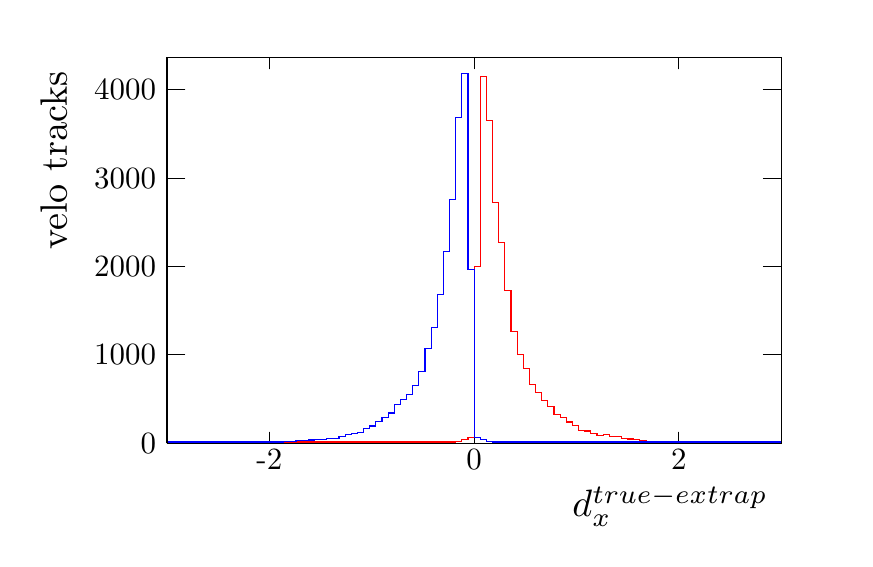
\begin{tikzpicture}
\pgfdeclareplotmark{cross} {
\pgfpathmoveto{\pgfpoint{-0.3\pgfplotmarksize}{\pgfplotmarksize}}
\pgfpathlineto{\pgfpoint{+0.3\pgfplotmarksize}{\pgfplotmarksize}}
\pgfpathlineto{\pgfpoint{+0.3\pgfplotmarksize}{0.3\pgfplotmarksize}}
\pgfpathlineto{\pgfpoint{+1\pgfplotmarksize}{0.3\pgfplotmarksize}}
\pgfpathlineto{\pgfpoint{+1\pgfplotmarksize}{-0.3\pgfplotmarksize}}
\pgfpathlineto{\pgfpoint{+0.3\pgfplotmarksize}{-0.3\pgfplotmarksize}}
\pgfpathlineto{\pgfpoint{+0.3\pgfplotmarksize}{-1.\pgfplotmarksize}}
\pgfpathlineto{\pgfpoint{-0.3\pgfplotmarksize}{-1.\pgfplotmarksize}}
\pgfpathlineto{\pgfpoint{-0.3\pgfplotmarksize}{-0.3\pgfplotmarksize}}
\pgfpathlineto{\pgfpoint{-1.\pgfplotmarksize}{-0.3\pgfplotmarksize}}
\pgfpathlineto{\pgfpoint{-1.\pgfplotmarksize}{0.3\pgfplotmarksize}}
\pgfpathlineto{\pgfpoint{-0.3\pgfplotmarksize}{0.3\pgfplotmarksize}}
\pgfpathclose
\pgfusepathqstroke
}
\pgfdeclareplotmark{cross*} {
\pgfpathmoveto{\pgfpoint{-0.3\pgfplotmarksize}{\pgfplotmarksize}}
\pgfpathlineto{\pgfpoint{+0.3\pgfplotmarksize}{\pgfplotmarksize}}
\pgfpathlineto{\pgfpoint{+0.3\pgfplotmarksize}{0.3\pgfplotmarksize}}
\pgfpathlineto{\pgfpoint{+1\pgfplotmarksize}{0.3\pgfplotmarksize}}
\pgfpathlineto{\pgfpoint{+1\pgfplotmarksize}{-0.3\pgfplotmarksize}}
\pgfpathlineto{\pgfpoint{+0.3\pgfplotmarksize}{-0.3\pgfplotmarksize}}
\pgfpathlineto{\pgfpoint{+0.3\pgfplotmarksize}{-1.\pgfplotmarksize}}
\pgfpathlineto{\pgfpoint{-0.3\pgfplotmarksize}{-1.\pgfplotmarksize}}
\pgfpathlineto{\pgfpoint{-0.3\pgfplotmarksize}{-0.3\pgfplotmarksize}}
\pgfpathlineto{\pgfpoint{-1.\pgfplotmarksize}{-0.3\pgfplotmarksize}}
\pgfpathlineto{\pgfpoint{-1.\pgfplotmarksize}{0.3\pgfplotmarksize}}
\pgfpathlineto{\pgfpoint{-0.3\pgfplotmarksize}{0.3\pgfplotmarksize}}
\pgfpathclose
\pgfusepathqfillstroke
}
\pgfdeclareplotmark{newstar} {
\pgfpathmoveto{\pgfqpoint{0pt}{\pgfplotmarksize}}
\pgfpathlineto{\pgfqpointpolar{44}{0.5\pgfplotmarksize}}
\pgfpathlineto{\pgfqpointpolar{18}{\pgfplotmarksize}}
\pgfpathlineto{\pgfqpointpolar{-20}{0.5\pgfplotmarksize}}
\pgfpathlineto{\pgfqpointpolar{-54}{\pgfplotmarksize}}
\pgfpathlineto{\pgfqpointpolar{-90}{0.5\pgfplotmarksize}}
\pgfpathlineto{\pgfqpointpolar{234}{\pgfplotmarksize}}
\pgfpathlineto{\pgfqpointpolar{198}{0.5\pgfplotmarksize}}
\pgfpathlineto{\pgfqpointpolar{162}{\pgfplotmarksize}}
\pgfpathlineto{\pgfqpointpolar{134}{0.5\pgfplotmarksize}}
\pgfpathclose
\pgfusepathqstroke
}
\pgfdeclareplotmark{newstar*} {
\pgfpathmoveto{\pgfqpoint{0pt}{\pgfplotmarksize}}
\pgfpathlineto{\pgfqpointpolar{44}{0.5\pgfplotmarksize}}
\pgfpathlineto{\pgfqpointpolar{18}{\pgfplotmarksize}}
\pgfpathlineto{\pgfqpointpolar{-20}{0.5\pgfplotmarksize}}
\pgfpathlineto{\pgfqpointpolar{-54}{\pgfplotmarksize}}
\pgfpathlineto{\pgfqpointpolar{-90}{0.5\pgfplotmarksize}}
\pgfpathlineto{\pgfqpointpolar{234}{\pgfplotmarksize}}
\pgfpathlineto{\pgfqpointpolar{198}{0.5\pgfplotmarksize}}
\pgfpathlineto{\pgfqpointpolar{162}{\pgfplotmarksize}}
\pgfpathlineto{\pgfqpointpolar{134}{0.5\pgfplotmarksize}}
\pgfpathclose
\pgfusepathqfillstroke
}
\definecolor{c}{rgb}{1,1,1};
\draw [color=c, fill=c] (0,0) rectangle (10,6.27517);
\draw [color=c, fill=c] (1.4,1.00403) rectangle (9.2,5.89866);
\definecolor{c}{rgb}{0,0,0};
\draw [c] (1.4,1.00403) -- (1.4,5.89866) -- (9.2,5.89866) -- (9.2,1.00403) -- (1.4,1.00403);
\definecolor{c}{rgb}{1,1,1};
\draw [color=c, fill=c] (1.4,1.00403) rectangle (9.2,5.89866);
\definecolor{c}{rgb}{0,0,0};
\draw [c] (1.4,1.00403) -- (1.4,5.89866) -- (9.2,5.89866) -- (9.2,1.00403) -- (1.4,1.00403);
\definecolor{c}{rgb}{1,0,0};
\draw [c,line width=0.4] (1.41678,1.02081) -- (1.41678,1.02081) -- (1.478,1.02081) -- (1.478,1.02081) -- (1.556,1.02081) -- (1.556,1.02081) -- (1.634,1.02081) -- (1.634,1.02081) -- (1.712,1.02081) -- (1.712,1.02081) -- (1.79,1.02081) --
 (1.79,1.02081) -- (1.868,1.02081) -- (1.868,1.02081) -- (1.946,1.02081) -- (1.946,1.02081) -- (2.024,1.02081) -- (2.024,1.02081) -- (2.102,1.02081) -- (2.102,1.02081) -- (2.18,1.02081) -- (2.18,1.02081) -- (2.258,1.02081) -- (2.258,1.02081) --
 (2.336,1.02081) -- (2.336,1.02081) -- (2.414,1.02081) -- (2.414,1.02081) -- (2.492,1.02081) -- (2.492,1.02081) -- (2.57,1.02081) -- (2.57,1.02081) -- (2.648,1.02081) -- (2.648,1.02081) -- (2.726,1.02081) -- (2.726,1.02081) -- (2.804,1.02081) --
 (2.804,1.02081) -- (2.882,1.02081) -- (2.882,1.02081) -- (2.96,1.02081) -- (2.96,1.02081) -- (3.038,1.02081) -- (3.038,1.02081) -- (3.116,1.02081) -- (3.116,1.02081) -- (3.194,1.02081) -- (3.194,1.02081) -- (3.272,1.02081) -- (3.272,1.02081) --
 (3.35,1.02081) -- (3.35,1.02081) -- (3.428,1.02081) -- (3.428,1.02081) -- (3.506,1.02081) -- (3.506,1.02081) -- (3.584,1.02081) -- (3.584,1.02081) -- (3.662,1.02081) -- (3.662,1.02081) -- (3.74,1.02081) -- (3.74,1.02081) -- (3.818,1.02081) --
 (3.818,1.02081) -- (3.896,1.02081) -- (3.896,1.02081) -- (3.974,1.02081) -- (3.974,1.02081) -- (4.052,1.02081) -- (4.052,1.02081) -- (4.13,1.02081) -- (4.13,1.02081) -- (4.208,1.02081) -- (4.208,1.02081) -- (4.286,1.02081) -- (4.286,1.02081) --
 (4.364,1.02081) -- (4.364,1.02081) -- (4.442,1.02081) -- (4.442,1.02081) -- (4.52,1.02081) -- (4.52,1.02081) -- (4.598,1.02081) -- (4.598,1.02081) -- (4.676,1.02081) -- (4.676,1.02081) -- (4.754,1.02081) -- (4.754,1.02081) -- (4.832,1.02081) --
 (4.832,1.02081) -- (4.91,1.02081) -- (4.91,1.02081) -- (4.988,1.02081) -- (4.988,1.02081) -- (5.066,1.02081) -- (5.066,1.02423) -- (5.144,1.02423) -- (5.144,1.05116) -- (5.222,1.05116) -- (5.222,1.07697) -- (5.3,1.07697) -- (5.3,3.25176) --
 (5.378,3.25176) -- (5.378,5.66558) -- (5.456,5.66558) -- (5.456,5.10112) -- (5.534,5.10112) -- (5.534,4.06086) -- (5.612,4.06086) -- (5.612,3.55475) -- (5.69,3.55475) -- (5.69,2.93979) -- (5.768,2.93979) -- (5.768,2.41798) -- (5.846,2.41798) --
 (5.846,2.12846) -- (5.924,2.12846) -- (5.924,1.95003) -- (6.002,1.95003) -- (6.002,1.74691) -- (6.08,1.74691) -- (6.08,1.64816) -- (6.158,1.64816) -- (6.158,1.55053) -- (6.236,1.55053) -- (6.236,1.47534) -- (6.314,1.47534) -- (6.314,1.36649) --
 (6.392,1.36649) -- (6.392,1.3317) -- (6.47,1.3317) -- (6.47,1.27447) -- (6.548,1.27447) -- (6.548,1.22622) -- (6.626,1.22622) -- (6.626,1.17011) -- (6.704,1.17011) -- (6.704,1.16001) -- (6.782,1.16001) -- (6.782,1.12859) -- (6.86,1.12859) --
 (6.86,1.1039) -- (6.938,1.1039) -- (6.938,1.11063) -- (7.016,1.11063) -- (7.016,1.08482) -- (7.094,1.08482) -- (7.094,1.08819) -- (7.172,1.08819) -- (7.172,1.06014) -- (7.25,1.06014) -- (7.25,1.05789) -- (7.328,1.05789) -- (7.328,1.0534) --
 (7.406,1.0534) -- (7.406,1.03769) -- (7.484,1.03769) -- (7.484,1.02871) -- (7.562,1.02871) -- (7.562,1.03096) -- (7.64,1.03096) -- (7.64,1.02081) -- (7.718,1.02081) -- (7.718,1.02081) -- (7.796,1.02081) -- (7.796,1.02081) -- (7.874,1.02081) --
 (7.874,1.02081) -- (7.952,1.02081) -- (7.952,1.02081) -- (8.03,1.02081) -- (8.03,1.02081) -- (8.108,1.02081) -- (8.108,1.02081) -- (8.186,1.02081) -- (8.186,1.02081) -- (8.264,1.02081) -- (8.264,1.02081) -- (8.342,1.02081) -- (8.342,1.02081) --
 (8.42,1.02081) -- (8.42,1.02081) -- (8.498,1.02081) -- (8.498,1.02081) -- (8.576,1.02081) -- (8.576,1.02081) -- (8.654,1.02081) -- (8.654,1.02081) -- (8.732,1.02081) -- (8.732,1.02081) -- (8.81,1.02081) -- (8.81,1.02081) -- (8.888,1.02081) --
 (8.888,1.02081) -- (8.966,1.02081) -- (8.966,1.02081) -- (9.044,1.02081) -- (9.044,1.02081) -- (9.122,1.02081) -- (9.122,1.02081) -- (9.2,1.02081);
\definecolor{c}{rgb}{0,0,0};
\draw [c,line width=0.4] (1.4,1.00403) -- (9.2,1.00403);
\draw [anchor= east] (9.2,0.200805) node[scale=1.37879, rotate=0]{$d_{x}^{true-extrap}$};
\draw [c,line width=0.4] (2.7,1.15087) -- (2.7,1.00403);
\draw [c,line width=0.4] (5.3,1.15087) -- (5.3,1.00403);
\draw [c,line width=0.4] (7.9,1.15087) -- (7.9,1.00403);
\draw [c,line width=0.4] (2.7,1.15087) -- (2.7,1.00403);
\draw [c,line width=0.4] (7.9,1.15087) -- (7.9,1.00403);
\draw [anchor=base] (2.7,0.665168) node[scale=1.11794, rotate=0]{-2};
\draw [anchor=base] (5.3,0.665168) node[scale=1.11794, rotate=0]{0};
\draw [anchor=base] (7.9,0.665168) node[scale=1.11794, rotate=0]{2};
\draw [c,line width=0.4] (1.4,5.89866) -- (9.2,5.89866);
\draw [c,line width=0.4] (2.7,5.75182) -- (2.7,5.89866);
\draw [c,line width=0.4] (5.3,5.75182) -- (5.3,5.89866);
\draw [c,line width=0.4] (7.9,5.75182) -- (7.9,5.89866);
\draw [c,line width=0.4] (2.7,5.75182) -- (2.7,5.89866);
\draw [c,line width=0.4] (7.9,5.75182) -- (7.9,5.89866);
\draw [c,line width=0.4] (1.4,1.00403) -- (1.4,5.89866);
\draw [anchor= east] (-0.04,5.89866) node[scale=1.37879, rotate=90]{velo tracks};
\draw [c,line width=0.4] (1.634,1.00403) -- (1.4,1.00403);
\draw [c,line width=0.4] (1.634,2.12621) -- (1.4,2.12621);
\draw [c,line width=0.4] (1.634,3.2484) -- (1.4,3.2484);
\draw [c,line width=0.4] (1.634,4.37058) -- (1.4,4.37058);
\draw [c,line width=0.4] (1.634,5.49276) -- (1.4,5.49276);
\draw [c,line width=0.4] (1.634,5.49276) -- (1.4,5.49276);
\draw [anchor= east] (1.4,1.00403) node[scale=1.11794, rotate=0]{0};
\draw [anchor= east] (1.4,2.12621) node[scale=1.11794, rotate=0]{1000};
\draw [anchor= east] (1.4,3.2484) node[scale=1.11794, rotate=0]{2000};
\draw [anchor= east] (1.4,4.37058) node[scale=1.11794, rotate=0]{3000};
\draw [anchor= east] (1.4,5.49276) node[scale=1.11794, rotate=0]{4000};
\draw [c,line width=0.4] (9.2,1.00403) -- (9.2,5.89866);
\draw [c,line width=0.4] (8.966,1.00403) -- (9.2,1.00403);
\draw [c,line width=0.4] (8.966,2.12621) -- (9.2,2.12621);
\draw [c,line width=0.4] (8.966,3.2484) -- (9.2,3.2484);
\draw [c,line width=0.4] (8.966,4.37058) -- (9.2,4.37058);
\draw [c,line width=0.4] (8.966,5.49276) -- (9.2,5.49276);
\draw [c,line width=0.4] (8.966,5.49276) -- (9.2,5.49276);
\definecolor{c}{rgb}{0,0,1};
\draw [c,line width=0.4] (1.41678,1.02081) -- (1.41678,1.02081) -- (1.478,1.02081) -- (1.478,1.02081) -- (1.556,1.02081) -- (1.556,1.02081) -- (1.634,1.02081) -- (1.634,1.02081) -- (1.712,1.02081) -- (1.712,1.02081) -- (1.79,1.02081) --
 (1.79,1.02081) -- (1.868,1.02081) -- (1.868,1.02081) -- (1.946,1.02081) -- (1.946,1.02081) -- (2.024,1.02081) -- (2.024,1.02081) -- (2.102,1.02081) -- (2.102,1.02081) -- (2.18,1.02081) -- (2.18,1.02081) -- (2.258,1.02081) -- (2.258,1.02081) --
 (2.336,1.02081) -- (2.336,1.02081) -- (2.414,1.02081) -- (2.414,1.02081) -- (2.492,1.02081) -- (2.492,1.02081) -- (2.57,1.02081) -- (2.57,1.02081) -- (2.648,1.02081) -- (2.648,1.02081) -- (2.726,1.02081) -- (2.726,1.02081) -- (2.804,1.02081) --
 (2.804,1.02081) -- (2.882,1.02081) -- (2.882,1.02198) -- (2.96,1.02198) -- (2.96,1.02759) -- (3.038,1.02759) -- (3.038,1.03433) -- (3.116,1.03433) -- (3.116,1.03881) -- (3.194,1.03881) -- (3.194,1.04555) -- (3.272,1.04555) -- (3.272,1.04667) --
 (3.35,1.04667) -- (3.35,1.05677) -- (3.428,1.05677) -- (3.428,1.07024) -- (3.506,1.07024) -- (3.506,1.06014) -- (3.584,1.06014) -- (3.584,1.08819) -- (3.662,1.08819) -- (3.662,1.114) -- (3.74,1.114) -- (3.74,1.12522) -- (3.818,1.12522) --
 (3.818,1.1443) -- (3.896,1.1443) -- (3.896,1.18807) -- (3.974,1.18807) -- (3.974,1.22285) -- (4.052,1.22285) -- (4.052,1.28233) -- (4.13,1.28233) -- (4.13,1.32834) -- (4.208,1.32834) -- (4.208,1.38894) -- (4.286,1.38894) -- (4.286,1.49442) --
 (4.364,1.49442) -- (4.364,1.55614) -- (4.442,1.55614) -- (4.442,1.62123) -- (4.52,1.62123) -- (4.52,1.73569) -- (4.598,1.73569) -- (4.598,1.92085) -- (4.676,1.92085) -- (4.676,2.20252) -- (4.754,2.20252) -- (4.754,2.47297) -- (4.832,2.47297) --
 (4.832,2.89715) -- (4.91,2.89715) -- (4.91,3.44253) -- (4.988,3.44253) -- (4.988,4.10126) -- (5.066,4.10126) -- (5.066,5.14152) -- (5.144,5.14152) -- (5.144,5.70486) -- (5.222,5.70486) -- (5.222,3.21136) -- (5.3,3.21136) -- (5.3,1.07248) --
 (5.378,1.07248) -- (5.378,1.04779) -- (5.456,1.04779) -- (5.456,1.03096) -- (5.534,1.03096) -- (5.534,1.02081) -- (5.612,1.02081) -- (5.612,1.02081) -- (5.69,1.02081) -- (5.69,1.02081) -- (5.768,1.02081) -- (5.768,1.02081) -- (5.846,1.02081) --
 (5.846,1.02081) -- (5.924,1.02081) -- (5.924,1.02081) -- (6.002,1.02081) -- (6.002,1.02081) -- (6.08,1.02081) -- (6.08,1.02081) -- (6.158,1.02081) -- (6.158,1.02081) -- (6.236,1.02081) -- (6.236,1.02081) -- (6.314,1.02081) -- (6.314,1.02081) --
 (6.392,1.02081) -- (6.392,1.02081) -- (6.47,1.02081) -- (6.47,1.02081) -- (6.548,1.02081) -- (6.548,1.02081) -- (6.626,1.02081) -- (6.626,1.02081) -- (6.704,1.02081) -- (6.704,1.02081) -- (6.782,1.02081) -- (6.782,1.02081) -- (6.86,1.02081) --
 (6.86,1.02081) -- (6.938,1.02081) -- (6.938,1.02081) -- (7.016,1.02081) -- (7.016,1.02081) -- (7.094,1.02081) -- (7.094,1.02081) -- (7.172,1.02081) -- (7.172,1.02081) -- (7.25,1.02081) -- (7.25,1.02081) -- (7.328,1.02081) -- (7.328,1.02081) --
 (7.406,1.02081) -- (7.406,1.02081) -- (7.484,1.02081) -- (7.484,1.02081) -- (7.562,1.02081) -- (7.562,1.02081) -- (7.64,1.02081) -- (7.64,1.02081) -- (7.718,1.02081) -- (7.718,1.02081) -- (7.796,1.02081) -- (7.796,1.02081) -- (7.874,1.02081) --
 (7.874,1.02081) -- (7.952,1.02081) -- (7.952,1.02081) -- (8.03,1.02081) -- (8.03,1.02081) -- (8.108,1.02081) -- (8.108,1.02081) -- (8.186,1.02081) -- (8.186,1.02081) -- (8.264,1.02081) -- (8.264,1.02081) -- (8.342,1.02081) -- (8.342,1.02081) --
 (8.42,1.02081) -- (8.42,1.02081) -- (8.498,1.02081) -- (8.498,1.02081) -- (8.576,1.02081) -- (8.576,1.02081) -- (8.654,1.02081) -- (8.654,1.02081) -- (8.732,1.02081) -- (8.732,1.02081) -- (8.81,1.02081) -- (8.81,1.02081) -- (8.888,1.02081) --
 (8.888,1.02081) -- (8.966,1.02081) -- (8.966,1.02081) -- (9.044,1.02081) -- (9.044,1.02081) -- (9.122,1.02081) -- (9.122,1.02081) -- (9.2,1.02081);
\end{tikzpicture}
}
    \caption{}
    \label{mvm_pos_neg_x_norm}
  \end{subfigure}
  \caption{positive negative normalised x residuals. }
 \label{mvm_pos_neg_x_norm_comp}
\end{figure}

% \begin{figure}[h]
%   \centering
%   \begin{subfigure}{0.5\textwidth}
%     \tikzsetnextfilename{mvTTm_wind_eff_bra}
%     \scalebox{.6}{\begin{tikzpicture}
\pgfdeclareplotmark{cross} {
\pgfpathmoveto{\pgfpoint{-0.3\pgfplotmarksize}{\pgfplotmarksize}}
\pgfpathlineto{\pgfpoint{+0.3\pgfplotmarksize}{\pgfplotmarksize}}
\pgfpathlineto{\pgfpoint{+0.3\pgfplotmarksize}{0.3\pgfplotmarksize}}
\pgfpathlineto{\pgfpoint{+1\pgfplotmarksize}{0.3\pgfplotmarksize}}
\pgfpathlineto{\pgfpoint{+1\pgfplotmarksize}{-0.3\pgfplotmarksize}}
\pgfpathlineto{\pgfpoint{+0.3\pgfplotmarksize}{-0.3\pgfplotmarksize}}
\pgfpathlineto{\pgfpoint{+0.3\pgfplotmarksize}{-1.\pgfplotmarksize}}
\pgfpathlineto{\pgfpoint{-0.3\pgfplotmarksize}{-1.\pgfplotmarksize}}
\pgfpathlineto{\pgfpoint{-0.3\pgfplotmarksize}{-0.3\pgfplotmarksize}}
\pgfpathlineto{\pgfpoint{-1.\pgfplotmarksize}{-0.3\pgfplotmarksize}}
\pgfpathlineto{\pgfpoint{-1.\pgfplotmarksize}{0.3\pgfplotmarksize}}
\pgfpathlineto{\pgfpoint{-0.3\pgfplotmarksize}{0.3\pgfplotmarksize}}
\pgfpathclose
\pgfusepathqstroke
}
\pgfdeclareplotmark{cross*} {
\pgfpathmoveto{\pgfpoint{-0.3\pgfplotmarksize}{\pgfplotmarksize}}
\pgfpathlineto{\pgfpoint{+0.3\pgfplotmarksize}{\pgfplotmarksize}}
\pgfpathlineto{\pgfpoint{+0.3\pgfplotmarksize}{0.3\pgfplotmarksize}}
\pgfpathlineto{\pgfpoint{+1\pgfplotmarksize}{0.3\pgfplotmarksize}}
\pgfpathlineto{\pgfpoint{+1\pgfplotmarksize}{-0.3\pgfplotmarksize}}
\pgfpathlineto{\pgfpoint{+0.3\pgfplotmarksize}{-0.3\pgfplotmarksize}}
\pgfpathlineto{\pgfpoint{+0.3\pgfplotmarksize}{-1.\pgfplotmarksize}}
\pgfpathlineto{\pgfpoint{-0.3\pgfplotmarksize}{-1.\pgfplotmarksize}}
\pgfpathlineto{\pgfpoint{-0.3\pgfplotmarksize}{-0.3\pgfplotmarksize}}
\pgfpathlineto{\pgfpoint{-1.\pgfplotmarksize}{-0.3\pgfplotmarksize}}
\pgfpathlineto{\pgfpoint{-1.\pgfplotmarksize}{0.3\pgfplotmarksize}}
\pgfpathlineto{\pgfpoint{-0.3\pgfplotmarksize}{0.3\pgfplotmarksize}}
\pgfpathclose
\pgfusepathqfillstroke
}
\pgfdeclareplotmark{newstar} {
\pgfpathmoveto{\pgfqpoint{0pt}{\pgfplotmarksize}}
\pgfpathlineto{\pgfqpointpolar{44}{0.5\pgfplotmarksize}}
\pgfpathlineto{\pgfqpointpolar{18}{\pgfplotmarksize}}
\pgfpathlineto{\pgfqpointpolar{-20}{0.5\pgfplotmarksize}}
\pgfpathlineto{\pgfqpointpolar{-54}{\pgfplotmarksize}}
\pgfpathlineto{\pgfqpointpolar{-90}{0.5\pgfplotmarksize}}
\pgfpathlineto{\pgfqpointpolar{234}{\pgfplotmarksize}}
\pgfpathlineto{\pgfqpointpolar{198}{0.5\pgfplotmarksize}}
\pgfpathlineto{\pgfqpointpolar{162}{\pgfplotmarksize}}
\pgfpathlineto{\pgfqpointpolar{134}{0.5\pgfplotmarksize}}
\pgfpathclose
\pgfusepathqstroke
}
\pgfdeclareplotmark{newstar*} {
\pgfpathmoveto{\pgfqpoint{0pt}{\pgfplotmarksize}}
\pgfpathlineto{\pgfqpointpolar{44}{0.5\pgfplotmarksize}}
\pgfpathlineto{\pgfqpointpolar{18}{\pgfplotmarksize}}
\pgfpathlineto{\pgfqpointpolar{-20}{0.5\pgfplotmarksize}}
\pgfpathlineto{\pgfqpointpolar{-54}{\pgfplotmarksize}}
\pgfpathlineto{\pgfqpointpolar{-90}{0.5\pgfplotmarksize}}
\pgfpathlineto{\pgfqpointpolar{234}{\pgfplotmarksize}}
\pgfpathlineto{\pgfqpointpolar{198}{0.5\pgfplotmarksize}}
\pgfpathlineto{\pgfqpointpolar{162}{\pgfplotmarksize}}
\pgfpathlineto{\pgfqpointpolar{134}{0.5\pgfplotmarksize}}
\pgfpathclose
\pgfusepathqfillstroke
}
\definecolor{c}{rgb}{1,1,1};
\draw [color=c, fill=c] (0,0) rectangle (10,6.27517);
\draw [color=c, fill=c] (1.4,1.00403) rectangle (9.2,5.89866);
\definecolor{c}{rgb}{0,0,0};
\draw [c] (1.4,1.00403) -- (1.4,5.89866) -- (9.2,5.89866) -- (9.2,1.00403) -- (1.4,1.00403);
\definecolor{c}{rgb}{1,1,1};
\draw [color=c, fill=c] (1.4,1.00403) rectangle (9.2,5.89866);
\definecolor{c}{rgb}{0,0,0};
\draw [c] (1.4,1.00403) -- (1.4,5.89866) -- (9.2,5.89866) -- (9.2,1.00403) -- (1.4,1.00403);
\draw [c,line width=0.4] (1.4,1.00403) -- (9.2,1.00403);
\draw [anchor= east] (9.2,0.281128) node[scale=1.00614, rotate=0]{$d^{\text{M3}}_x$};
\draw [c,line width=0.4] (2.06922,1.15087) -- (2.06922,1.00403);
\draw [c,line width=0.4] (3.63491,1.15087) -- (3.63491,1.00403);
\draw [c,line width=0.4] (5.20059,1.15087) -- (5.20059,1.00403);
\draw [c,line width=0.4] (6.76628,1.15087) -- (6.76628,1.00403);
\draw [c,line width=0.4] (8.33196,1.15087) -- (8.33196,1.00403);
\draw [c,line width=0.4] (2.06922,1.15087) -- (2.06922,1.00403);
\draw [c,line width=0.4] (8.33196,1.15087) -- (8.33196,1.00403);
\draw [anchor=base] (2.06922,0.640067) node[scale=0.819821, rotate=0]{-2};
\draw [anchor=base] (3.63491,0.640067) node[scale=0.819821, rotate=0]{-1};
\draw [anchor=base] (5.20059,0.640067) node[scale=0.819821, rotate=0]{0};
\draw [anchor=base] (6.76628,0.640067) node[scale=0.819821, rotate=0]{1};
\draw [anchor=base] (8.33196,0.640067) node[scale=0.819821, rotate=0]{2};
\draw [c,line width=0.4] (1.4,5.89866) -- (9.2,5.89866);
\draw [c,line width=0.4] (2.06922,5.75182) -- (2.06922,5.89866);
\draw [c,line width=0.4] (3.63491,5.75182) -- (3.63491,5.89866);
\draw [c,line width=0.4] (5.20059,5.75182) -- (5.20059,5.89866);
\draw [c,line width=0.4] (6.76628,5.75182) -- (6.76628,5.89866);
\draw [c,line width=0.4] (8.33196,5.75182) -- (8.33196,5.89866);
\draw [c,line width=0.4] (2.06922,5.75182) -- (2.06922,5.89866);
\draw [c,line width=0.4] (8.33196,5.75182) -- (8.33196,5.89866);
\draw [c,line width=0.4] (1.4,1.00403) -- (1.4,5.89866);
\draw [anchor= east] (0.5936,5.89866) node[scale=1.00614, rotate=90]{$d^{\text{M3}}_y$};
\draw [c,line width=0.4] (1.634,1.8198) -- (1.4,1.8198);
\draw [c,line width=0.4] (1.634,3.45134) -- (1.4,3.45134);
\draw [c,line width=0.4] (1.634,5.08289) -- (1.4,5.08289);
\draw [c,line width=0.4] (1.634,1.8198) -- (1.4,1.8198);
\draw [c,line width=0.4] (1.634,5.08289) -- (1.4,5.08289);
\draw [anchor= east] (1.3,1.8198) node[scale=0.819821, rotate=0]{-2};
\draw [anchor= east] (1.3,3.45134) node[scale=0.819821, rotate=0]{0};
\draw [anchor= east] (1.3,5.08289) node[scale=0.819821, rotate=0]{2};
\draw [c,line width=0.4] (9.2,1.00403) -- (9.2,5.89866);
\draw [c,line width=0.4] (8.966,1.8198) -- (9.2,1.8198);
\draw [c,line width=0.4] (8.966,3.45134) -- (9.2,3.45134);
\draw [c,line width=0.4] (8.966,5.08289) -- (9.2,5.08289);
\draw [c,line width=0.4] (8.966,1.8198) -- (9.2,1.8198);
\draw [c,line width=0.4] (8.966,5.08289) -- (9.2,5.08289);
\foreach \P in
 {(5.51173,3.28593),(4.76591,3.42757),(5.66482,3.59951),(5.07651,3.5002),(5.05531,3.4871),(5.38096,3.50507),(3.51666,2.87207),(5.80893,3.52388),(4.19713,3.67934),(4.07722,3.25915),(5.52408,3.45134),(4.9194,3.5661),(4.86141,3.40473),(5.40714,3.48539),
(5.40955,3.43591),(4.97626,3.49906),(5.87938,3.54637),(4.63591,3.4863),(5.39136,3.42244),(4.10861,3.23044),(5.24068,3.41917),(5.02662,3.50504),(3.66969,3.12998),(5.47151,3.44371),(4.92239,3.41594),(6.57357,3.63031),(5.28603,3.46888),(5.03744,3.45458)
,(5.0572,3.43154),(4.85907,3.488),(5.64922,3.3723),(6.36018,3.54641),(5.3534,3.40956),(4.83121,3.50755),(5.35538,3.50774),(5.00523,3.39249),(4.73215,3.53805),(5.02205,3.50407),(5.40623,3.55438),(6.41053,3.28384),(5.64929,3.60542),(4.92194,3.35236),(5
.33012,3.43799),(4.76645,3.51037),(4.50456,3.40319),(5.6035,3.56282),(4.87208,3.48656),(5.36197,3.55212),(4.78066,3.36503),(5.13584,3.45663),(5.31572,3.43472),(4.19014,3.38126),(6.2491,3.55559),(5.344,3.44372),(4.74745,3.3769),(5.48932,3.44394),(4.27
877,3.43355),(5.10915,3.47751),(5.425,3.45812),(5.47053,3.47241),(4.49925,3.41753),(5.9596,3.38709),(5.85476,3.31302),(4.37947,3.43394),(5.08418,3.27149),(6.99133,3.39162),(5.49578,3.49806),(4.11617,3.32963),(5.29478,3.50266),(4.60097,3.34241),(6.200
04,3.64021),(5.48094,3.00362),(5.1113,3.24508),(5.46699,3.46656),(4.71356,3.29779),(4.08167,3.65479),(5.90542,3.51426),(5.32645,3.45904),(4.63382,3.45487),(6.12343,3.59762),(4.81767,3.46689),(4.77469,3.50924),(5.35805,3.60777),(5.45589,3.30237),(4.71
51,3.80526),(5.42198,3.38063),(3.83944,2.97492),(5.65596,3.35968),(5.12315,3.45048),(4.99222,3.54048),(5.73499,3.50668),(4.73745,3.47925),(5.42998,3.46091),(5.6017,3.50585),(4.26426,3.52773),(5.40822,3.52703),(4.78965,3.50062),(5.53839,3.45832),(4.97
862,3.39938),(5.69877,3.42114),(5.06882,3.47929),(5.46753,3.44842),(4.9186,3.56047),(4.74231,3.38448),(5.27022,3.51941),(4.84563,3.48143),(6.03263,3.6296),(6.05888,3.26495),(4.75526,3.44115),(4.71426,3.4239),(6.94429,3.41561),(4.86929,3.47665),(5.838
38,3.57958),(5.37651,3.49454),(5.1282,3.42045),(6.56047,3.39084),(4.89105,3.46129),(6.65367,3.27779),(6.76154,3.45165),(4.84432,3.51515),(4.8455,3.55201),(4.93626,3.43822),(7.4048,3.40845),(5.37513,3.39382),(3.66251,3.2495),(5.37345,3.46536),(4.47308
,3.58874),(6.73882,2.45402),(5.54795,3.34887),(4.58557,3.55254),(5.33999,3.53224),(4.89298,3.44243),(4.76909,3.48307),(5.40676,3.37521),(5.63944,3.5898),(4.84278,3.37748),(4.90949,3.51512),(5.35468,3.36122),(5.12327,3.45625),(5.4781,3.39855),(4.60249
,3.47408),(4.61992,3.49213),(5.19605,3.27662),(5.07374,3.46972),(4.40432,3.57784),(5.59693,3.62784),(5.75681,3.51038),(4.56757,3.48244),(5.4282,3.37948),(4.96729,3.5275),(5.02483,3.41391),(5.45351,3.38311),(5.55515,3.51029),(4.32073,3.41314),(5.15219
,3.4773),(5.32863,3.48986),(5.42702,3.43531),(2.63746,3.23334),(4.68717,3.35113),(6.41943,3.70108),(6.85822,3.68146),(3.93804,3.49296),(6.90938,3.57064),(4.72424,3.2555),(5.5183,3.50747),(7.47495,3.25191),(5.4045,3.55697),(3.19417,3.95165),(4.81236,3
.45542),(5.75425,3.50497),(6.85903,3.54201),(4.41432,3.23396),(5.31864,3.39928),(4.99894,3.45612),(5.48704,3.37976),(4.61487,3.46318),(5.09743,3.43183),(4.87809,3.57071),(5.13117,3.45118),(5.40886,3.68447),(5.3451,3.51354),(4.59328,3.28891),(5.50954,
3.61049),(4.03399,2.84636),(5.43138,3.44822),(5.38905,3.45526),(4.97262,3.48457),(5.12819,3.42365),(5.84756,3.59286),(5.41433,3.44036),(4.7988,3.38734),(3.25765,3.79786),(5.32557,3.4684),(4.93852,3.45207),(5.45058,3.46327),(6.58374,3.3801),(5.01365,3
.47099),(5.24734,3.31744),(5.09782,3.32359),(4.87787,3.33395),(5.63591,3.52371),(6.21032,3.64301),(5.03647,3.48639),(4.76454,3.2133),(6.50855,3.45109),(5.03429,3.42399),(5.5547,3.44927),(6.97343,3.44617),(3.87275,3.45427),(4.52789,3.39305),(4.80421,3
.36404),(5.54046,3.53391),(4.61308,3.48295),(6.26838,3.34346),(4.24504,3.12577),(5.06397,3.42489),(6.08442,3.39643),(5.34562,3.32239),(5.0984,3.42384),(5.65107,3.28381),(3.81434,3.52694),(4.97077,3.46792),(5.24241,3.46404),(5.15767,3.42162),(5.72974,
3.03623),(5.03217,3.42634),(5.34735,3.45546),(5.08879,3.5224),(5.35827,3.37919),(5.24976,3.51496),(5.16108,3.41705),(4.63107,3.37153),(5.46975,3.41051),(5.136,3.49595),(5.32456,3.42487),(5.45408,3.42609),(4.4902,3.34096),(4.27253,3.51437),(5.29996,3.
42165),(5.94379,3.36563),(5.11466,3.44159),(7.14618,3.5697),(4.92695,3.4458),(5.36536,3.45481),(5.31437,3.44146),(5.14959,3.49617),(6.5842,3.29861),(4.55431,3.61334),(5.68241,3.45313),(4.33479,3.46188),(5.70172,3.4406),(6.11534,3.43735),(4.93703,3.46
112),(4.94333,3.46131),(5.86754,3.35537),(5.86363,3.6286),(4.66771,3.43495),(5.68692,3.32271),(3.66328,3.59863),(5.6219,3.38237),(4.93074,3.45316),(4.11528,3.41452),(6.3105,3.1728),(4.85991,3.49263),(4.76949,3.41645),(4.82008,3.50518),(4.69862,3.3044
9),(6.37549,3.51769),(6.37701,3.65396),(3.01387,2.82144),(5.00013,3.43467),(5.34593,3.43523),(5.08263,3.47344),(6.38662,3.54554),(4.43589,3.41532),(6.69411,3.3442),(6.09748,3.8314),(4.36164,3.40396),(4.83741,3.51187),(5.5818,3.49041),(5.39313,3.49418
),(5.34116,3.55466),(5.10405,3.46046),(5.4913,3.47389),(4.86761,3.60588),(5.95396,3.60827),(4.19409,3.60559),(3.85223,3.20214),(5.41909,3.42499),(4.85266,3.39267),(5.30578,3.41698),(5.86444,3.34699),(3.35046,3.02629),(5.35077,3.43643),(3.13743,3.1053
8),(4.73659,3.45404),(5.36841,3.52345),(5.64147,3.66157),(4.60752,3.55248),(5.58378,3.43491),(3.62387,3.68779),(5.90277,3.41095),(4.09612,3.26675),(4.28185,3.72964),(5.59575,3.4251),(5.2551,3.47886),(5.65098,3.489),(5.00845,3.39609),(4.94169,3.32579)
,(5.02407,3.49025),(5.50084,3.5307),(5.31861,3.40365),(6.5989,4.09571),(4.66335,3.4842),(5.05964,3.45288),(5.36602,3.41247),(5.55676,3.4264),(5.01266,3.42072),(4.04068,3.36768),(5.85848,3.53106),(5.89361,3.20476),(4.81272,3.49051),(4.31797,3.36474),(
6.55458,3.41238),(5.38031,3.46291),(3.73595,3.46602),(5.35698,3.47577),(5.08631,3.44648),(4.44365,3.56944),(5.4053,3.38558),(4.10157,3.16357),(5.70371,3.43626),(4.74807,3.62595),(5.34745,3.47381),(5.37613,3.42716),(3.87492,3.00027),(4.40297,3.36462),
(5.26537,3.43919),(5.371,3.45514),(5.00379,3.44505),(4.71428,3.4844),(6.31136,3.42838),(5.30399,3.46997),(5.09705,3.59567),(4.00293,3.96101),(5.29943,3.44389),(4.92035,3.35623),(6.36091,3.60429),(4.85769,3.46872),(5.27851,3.45538),(5.69491,3.38393),(
4.76106,3.38858),(5.33179,3.39054),(4.68424,3.48241),(4.14256,3.49885),(6.00383,3.26528),(5.52024,3.47928),(4.15675,3.723),(4.99958,3.37775),(5.48214,3.33962),(5.50354,3.41004),(4.72239,3.5008),(5.05569,3.42484),(5.33369,3.50235),(4.70149,3.58581),(5
.46051,3.48455),(5.02232,3.40973),(5.12293,3.4985),(5.28424,3.49704),(5.30335,3.42609),(5.15382,3.3848),(5.03186,3.44939),(5.36565,3.68473),(4.76993,3.56734),(6.36404,3.68316),(6.8093,2.96878),(5.06519,3.50898),(5.04119,3.50896),(5.26174,3.46792),(4.
80945,3.54652),(4.0068,2.99518),(6.22843,3.53198),(4.65896,3.43036),(4.7749,3.45751),(5.37264,3.49223),(6.21439,3.36199),(4.32462,3.49247),(4.93984,3.39148),(5.2821,3.48285),(5.33832,3.42304),(5.12673,3.51358),(4.82167,3.40044),(5.57499,3.43172),(5.0
4211,3.40801),(6.05105,3.65418),(5.82988,3.47998),(5.10436,3.32887),(5.35702,3.55463),(4.2307,3.34713),(5.72792,3.47615),(6.15215,2.61448),(4.93524,3.30594),(4.99817,3.46707),(5.84081,3.52076),(5.87029,3.40778),(5.0755,3.46397),(5.03057,3.50833),(6.0
8879,3.80455),(3.62829,3.58006),(5.01246,3.51634),(5.33054,3.41199),(5.60757,3.41144),(3.96776,3.78328),(4.81449,3.55072),(6.38843,3.25382),(5.79201,3.37093),(5.12388,3.41726),(5.55634,3.5099),(4.807,3.41908),(5.37041,3.48259),(5.07531,3.49439),(3.80
579,3.01669),(5.02156,3.48354),(3.97104,3.78845),(5.28497,3.43622),(5.53814,3.49038),(5.41711,3.49501),(4.78146,3.4012),(4.94953,3.59101),(7.89698,2.8943),(6.41198,3.43532),(5.57507,3.47253),(3.91936,3.52576),(3.98753,3.65704),(5.48385,3.47426),(5.32
85,3.40483),(4.25543,3.48318),(5.41605,3.42535),(4.5669,3.42087),(5.62787,3.46945),(5.31742,3.42291),(5.08736,3.4609),(5.46915,3.47025),(6.34699,3.3486),(4.97647,3.4319),(4.86196,3.47979),(5.72717,3.55175),(5.72596,3.34367),(4.17838,3.47926),(4.76191
,3.38268),(5.32721,3.44596),(4.96164,3.40403),(5.29527,3.48064),(4.75367,3.50324),(5.90157,3.56444),(5.12904,3.5578),(5.73679,3.51888),(4.71979,3.36941),(5.53917,3.54886),(5.5099,3.4944),(4.81027,3.38816),(5.83992,3.42494),(5.03723,3.43416),(5.4694,3
.61182),(3.47656,3.33061),(5.08172,3.39741),(5.25447,3.50334),(4.8196,3.53507),(7.48717,3.36391),(5.01248,3.41333),(5.28955,3.46252),(5.82023,3.47819),(3.79034,3.69948),(5.01702,3.48789),(5.33612,3.4151),(5.42075,3.43665),(4.97785,3.4687),(5.43867,3.
58073),(4.862,3.53877),(4.53179,3.84214),(5.44089,3.75851),(4.8862,3.48962),(5.49624,3.56095),(4.90886,3.62456),(6.05281,3.4321),(5.14252,3.42317),(5.27087,3.47672),(5.1215,3.28921),(5.32944,3.48031),(5.8906,3.47874),(4.91601,3.49968),(5.45056,3.4735
3),(5.13646,3.33907),(5.59132,3.516),(4.95709,3.4357),(5.35022,3.43238),(5.9489,3.49879),(4.69603,3.60749),(4.97784,3.3353),(5.78329,3.54817),(4.44801,3.37919),(4.77333,3.54788),(5.32102,3.36749),(4.94261,3.44889),(5.45517,3.51898),(5.79809,3.25371),
(4.84854,3.41964),(5.46627,3.51316),(4.60433,3.46402),(5.13804,3.48586),(6.9744,3.66063),(6.48951,3.18994),(3.25306,3.18872),(4.18926,3.45202),(6.01634,3.56845),(4.70087,3.4853),(5.34252,3.41816),(6.26159,3.48969),(4.99154,3.59298),(5.25174,3.43977),
(5.1611,3.46903),(5.32576,3.47761),(5.03507,3.44682),(5.36746,3.43924),(4.4224,3.16832),(6.12033,3.88514),(5.79673,3.62572),(4.89496,3.40609),(5.30687,3.47216),(4.54379,3.46103),(5.40478,3.39756),(4.84707,3.46747),(5.45027,3.42067),(4.54498,3.54121),
(4.50284,3.33355),(5.60434,3.45891),(5.3183,3.41902),(5.09884,3.52008),(4.98297,3.29139),(5.30947,3.55594),(5.05534,3.42055),(5.0442,3.51571),(4.78778,3.43004),(5.50186,3.51064),(3.55878,3.16827),(5.32563,3.30619),(6.37084,3.61286),(4.66139,3.37443),
(3.96257,3.35727),(5.51225,3.46198),(5.29003,3.32944),(4.86278,3.43632),(3.79738,3.40115),(5.48375,3.44963),(5.13413,3.45958),(5.30377,3.47634),(5.61952,3.39854),(4.65625,3.41243),(5.81404,3.33634),(5.09275,3.61158),(4.96758,3.42677),(5.49376,3.53121
),(5.13027,3.4949),(5.79799,3.32989),(4.89701,3.434),(5.10064,3.45879),(5.12641,3.4466),(4.53529,3.50441),(5.21834,3.5672),(4.84986,3.52722),(5.47945,3.48879),(4.8304,3.45508),(3.70887,3.81752),(5.54153,3.4682),(6.02499,3.55171),(4.5424,3.45601),(4.4
5143,3.46972),(5.28711,3.37213),(5.40012,3.47802),(4.71919,3.57262),(5.10939,3.51815),(6.36904,3.92358),(3.68605,3.14722),(4.32874,3.46223),(5.30055,3.46767),(4.95561,3.41706),(5.68646,3.57497),(4.74858,3.37579),(7.13099,3.00067),(4.89026,3.38483),(5
.29428,3.42006),(5.11769,3.52454),(4.03429,3.13024),(6.11397,3.71516),(3.58794,3.58966),(6.63575,3.4749),(4.91799,3.51163),(5.11492,3.24768),(5.2841,3.42185),(5.52934,3.47359),(4.50423,3.36322),(5.1448,3.47585),(4.95989,3.60788),(5.95048,3.48006),(5.
14049,3.34646),(6.04171,3.75271),(5.64337,3.21226),(4.94022,3.43333),(7.09755,3.26833),(6.27924,3.68206),(5.0447,3.4281),(5.60991,3.53245),(4.76119,3.4571),(5.30244,3.5072),(5.12515,3.4023),(4.94957,3.56256),(5.44838,3.55824),(6.84543,2.30086),(4.410
16,3.52962),(5.23111,3.42203),(4.5873,3.49946),(5.32335,3.50174),(5.06277,3.39168),(5.47576,3.43777),(5.33934,3.50133),(5.00367,3.47768),(4.67301,3.44899),(5.35896,3.38402),(5.16108,3.42346),(3.32404,3.42408),(5.46215,3.42429),(5.73078,3.40502),(4.63
017,3.52074),(4.82963,3.37635),(5.43596,3.4591),(5.82706,3.4743),(5.06242,3.42906),(5.16712,3.26506),(4.78624,3.49139),(4.84711,3.36386),(5.44306,3.40556),(4.81788,3.48597),(3.66972,3.72156),(5.60518,3.47107),(5.4709,3.50728),(4.87854,3.47981),(6.208
26,3.51248),(3.71033,3.36318),(5.49813,3.4687),(4.98939,3.48813),(5.2924,3.50357),(5.10554,3.46707),(5.32623,3.44799),(4.30825,3.28524),(5.70049,3.42441),(5.00952,3.39125),(5.42796,3.40528),(4.82124,3.61655),(5.8261,3.5285),(4.53293,3.34883),(5.3031,
3.31142),(4.75393,3.48944),(5.49187,3.44329),(5.06031,3.46165),(5.35859,3.65205),(4.89646,3.4061),(5.65014,3.53674),(4.20614,3.43414),(4.60695,3.51652),(4.69866,3.3537),(5.35533,3.54994),(5.40912,3.44205),(4.78602,3.51384),(5.28934,3.40737),(4.57955,
3.41566),(3.74583,3.28301),(6.03741,3.44703),(4.41524,3.42136),(4.81401,3.43219),(5.86034,3.50341),(3.19947,3.72403),(4.43555,3.28943),(5.31857,3.41969),(4.83153,3.4634),(6.02069,3.8532),(3.95354,3.29633),(5.53195,3.3259),(5.00381,3.32071),(5.93882,3
.20004),(3.99789,3.46054),(5.75337,3.38863),(4.74338,3.36006),(5.6871,3.44913),(5.37995,3.4887),(4.93033,3.52521),(4.83839,3.33759),(5.63024,3.48836),(3.65671,3.57667),(5.13065,3.45661),(5.61847,3.53334),(4.30302,3.73988),(5.02752,3.4318),(6.76971,3.
11191),(5.64015,3.52763),(5.06543,3.48814),(3.9345,3.46743),(6.48151,3.45121),(5.66478,3.51939),(5.2398,3.44893),(5.1145,3.40168),(4.99697,3.73854),(5.42191,3.46254),(6.31503,3.81208),(4.77043,3.48478),(5.99333,3.41505),(4.89991,3.51684),(5.17724,3.4
4138),(5.04565,3.48796),(5.33065,3.49464),(4.69795,3.47633),(5.26824,3.45012),(5.17517,3.44711),(5.16249,3.42358),(5.36422,3.41262),(5.27838,3.33996),(4.68242,3.40226),(3.88664,3.9099),(5.9995,3.43305),(5.31634,3.47944),(5.11664,3.49509),(4.93094,3.3
3071),(5.60179,3.39238),(4.68522,3.36856),(7.04112,3.33184),(5.6678,3.44084),(4.9295,3.43752),(5.28134,3.41589),(4.4136,3.34526),(5.5128,3.37106),(4.73924,3.47423),(4.33532,3.26922),(5.39028,3.45184),(4.3605,2.94966),(5.43145,3.3133),(4.93454,3.39712
),(5.32397,3.48303),(4.90046,3.43284),(5.03489,3.44298),(5.34541,3.51137),(5.75074,3.23306),(4.43607,3.51998),(4.29333,3.29078),(4.84752,3.48033),(5.58926,3.37976),(5.03956,3.49181),(7.26796,2.95089),(4.63628,3.62182),(6.18693,3.54586),(5.15706,3.483
31),(4.54048,3.51882),(6.20772,3.29391),(3.59599,2.9976),(6.11664,3.55351),(5.06414,3.43512),(5.29352,3.51293),(5.15448,3.47886),(5.25449,3.41279),(5.13105,3.45426),(5.39798,3.4637),(5.46973,3.45258),(5.41249,3.38764),(4.91458,3.47828),(6.07012,3.308
81),(4.28161,3.50568),(5.54129,3.55093),(6.5719,3.53063),(4.50958,3.62395),(5.60188,3.41585),(4.75743,3.36717),(5.82268,3.77519),(5.30039,3.47624),(4.67078,3.41697),(5.72818,3.49357),(4.2163,4.07501),(4.88331,3.54205),(5.53081,3.40632),(4.67054,3.456
54),(5.93249,3.27701),(4.97385,3.52451),(6.34805,3.53136),(4.13619,3.71659),(5.72875,3.41261),(4.946,3.49523),(4.63485,3.58122),(5.35355,3.47309),(4.97915,3.42985),(5.28343,3.41693),(4.22335,3.74118),(5.7909,3.53042),(5.02289,3.41177),(5.57403,3.2610
9),(4.30967,3.9256),(5.29213,3.65918),(4.9365,3.4994),(5.37868,3.46403),(5.72247,3.50908),(6.35446,2.93478),(5.45072,3.42654),(5.38862,3.44203),(6.4018,3.71085),(5.08867,3.51555),(4.41562,3.38484),(5.70382,3.52533),(5.60905,3.47426),(4.00448,3.56993)
,(5.38927,3.35305),(4.85184,3.18599),(4.0516,3.43019),(5.79554,3.38186),(5.27071,3.43808),(5.10879,3.47422),(5.70973,3.4217),(4.7669,3.41628),(4.6746,3.48885),(5.36455,3.45378),(2.90206,3.81819),(6.10991,3.2866),(3.97789,3.52361),(5.55439,3.54988),(5
.75967,3.39277),(4.98462,3.44551),(4.42303,3.49766),(5.5216,3.35469),(5.79698,3.47524),(4.57306,3.5272),(4.26913,3.6431),(5.37034,3.4406),(5.39467,3.41794),(4.6221,3.71303),(5.149,3.44209),(5.34795,3.3963),(5.12023,3.41128),(4.86343,3.28088),(5.70904
,3.35556),(5.41286,3.44834),(5.08534,3.45334),(4.67735,3.409),(5.53286,3.45429),(5.38225,3.59466),(5.11684,3.21394),(4.72597,3.49557),(5.53558,3.5641),(5.12749,3.49576),(5.43792,3.41829),(4.96377,3.38901),(5.8257,3.52749),(5.35753,3.47918),(5.16289,3
.51193),(3.92312,4.28913),(5.76969,3.4038),(6.01777,3.49378),(5.0562,3.25465),(5.59875,3.42839),(4.03914,3.89574),(5.07674,3.47484),(5.3922,3.39673),(4.69817,3.48534),(6.37285,3.64062),(5.33933,3.43883),(5.00427,3.49453),(5.6965,3.46827),(4.94097,3.5
6251),(5.39359,3.38083),(4.49705,3.50759),(3.90809,3.28086),(4.88437,3.386),(5.28271,3.44611),(5.58941,3.38416),(4.81831,3.45285),(5.28577,3.49599),(5.00531,3.33212),(6.81351,3.6736),(6.22609,3.42148),(4.59109,3.30463),(5.07575,3.51666),(5.73949,3.63
344),(5.69319,3.37916),(4.80866,3.6146),(5.43458,3.44762),(3.01478,3.311),(3.12022,3.77337),(5.86453,3.33872),(5.36585,3.49108),(5.03717,3.45898),(5.09838,3.51195),(5.29671,3.49862),(4.63525,3.59378),(6.5229,3.30088),(4.17525,3.5792),(5.7679,3.66722)
,(5.89442,3.2054),(4.52391,3.55838),(4.23332,3.59725),(5.64413,3.53061),(4.08528,3.12922),(5.70243,3.48758),(3.87864,3.56965),(5.00871,3.49802),(6.28548,3.25298),(5.32021,3.44151),(5.1059,3.42419),(4.9619,3.38473),(5.47097,3.40166),(5.8683,3.55953),(
4.49511,3.46582),(4.90672,3.45335),(7.32749,4.00757),(5.45996,3.58133),(4.70152,3.44045),(5.42191,3.53137),(5.00008,3.53461),(4.69674,3.28323),(6.82059,3.40988),(5.68509,3.23215),(5.40517,3.45575),(4.84039,3.39266),(5.39393,3.40213),(4.89815,3.2681),
(5.65557,3.45873),(5.05156,3.45379),(6.52784,3.46358),(5.10358,3.40602),(5.58414,3.47996),(4.94389,3.48287),(6.1114,3.76704),(4.67236,3.44719),(5.73171,3.45765),(2.73031,3.45829),(4.90535,3.40852),(5.64755,3.43423),(4.6809,3.4705),(5.26678,3.43248),(
4.99313,3.43077),(4.87375,3.54957),(5.47748,3.50685),(6.67504,3.58929),(4.62321,3.61387),(4.45142,3.23424),(5.57096,3.37136),(4.89671,3.33425),(4.74477,3.34926),(5.91528,3.68392),(5.12814,3.50712),(7.58917,3.7722),(5.71658,3.56331),(5.04541,3.46625),
(4.8408,3.36575),(6.07707,3.78453),(4.77642,3.40081),(3.99748,3.56022),(5.92121,3.2127),(6.06846,3.50534),(6.89603,3.4736),(4.48906,3.21853),(5.49803,3.40298),(5.661,3.48722),(4.94838,3.58067),(5.36292,3.51859),(4.56251,3.40594),(6.15744,3.36205),(5.
75516,3.35784),(4.2845,3.35568),(5.68508,3.42774),(4.95055,3.32156),(6.12171,3.50658),(5.05082,3.40381),(3.93869,3.34183),(5.55195,3.45405),(4.41276,3.54864),(5.50146,3.47066),(4.83082,3.50618),(5.7739,3.45295),(5.21278,3.67711),(5.29352,3.41642),(5.
4853,3.42311),(6.02204,3.44063),(4.81718,3.43233),(5.62424,3.46646),(4.89303,3.40097),(5.49139,3.4847),(5.09842,3.46914),(5.50498,3.50003),(4.95711,3.40779),(4.97884,3.48481),(5.49124,3.46554),(5.13531,3.44856),(6.00318,3.20192),(3.35138,3.62042),(5.
02822,3.52305),(5.3215,3.45856),(4.7826,3.511),(6.4056,3.25295),(4.96888,3.52674),(6.63918,3.4795),(3.83741,3.53232),(4.89096,3.46596),(5.25484,3.48227),(4.97104,3.33949),(4.91455,3.51885),(5.6402,3.33413),(4.19654,3.45844),(5.24254,3.46091),(5.47456
,3.45123),(7.74726,3.06382),(4.5397,3.53642),(4.28673,3.14464),(6.72114,3.04784),(5.04621,3.43674),(5.54469,3.51095),(5.29935,3.54722),(5.03947,3.50624),(5.86277,3.37683),(4.85165,3.40489),(4.21831,3.52943),(5.55018,3.39392),(4.90731,3.43556),(5.9273
6,3.55283),(6.46326,3.3587),(3.94331,3.322),(4.87161,3.39846),(4.24829,3.39124),(5.33036,3.4251),(3.52587,3.50129),(5.83565,3.34431),(4.57729,3.33903),(5.40389,3.35928),(6.25526,3.32895),(4.26221,3.04447),(5.227,3.55966),(4.60173,3.45341),(4.38721,3.
59181),(5.49817,3.46997),(5.07177,3.44795),(5.5368,3.36524),(4.97542,3.37111),(6.09705,3.70433),(4.59596,3.57149),(6.16747,3.60059),(5.65453,3.39716),(5.03789,3.47949),(6.85376,3.8728),(5.07689,3.43519),(5.07388,3.52314),(5.31657,3.42693),(5.1399,3.4
8872),(5.47921,3.5013),(5.50286,3.46979),(5.00361,3.49339),(4.80118,3.41879),(5.40129,3.50618),(5.05573,3.40679),(5.28265,3.46724),(4.93628,3.53038),(5.36365,3.45662),(4.87444,3.45943),(5.4721,3.50568),(4.49479,3.48812),(5.5755,3.23478),(5.05497,3.51
237),(4.94271,3.5022),(6.72994,3.01236),(5.05125,3.50136),(5.88361,3.54785),(5.0285,3.37004),(6.46672,3.27884),(3.85897,3.34381),(4.73185,3.55376),(5.84193,3.43296),(4.92537,3.40992),(6.29363,3.3223),(6.15945,3.18686),(4.45571,3.45714),(5.22827,3.260
16),(5.34658,3.38081),(6.98157,3.09291),(6.02793,3.51841),(4.61927,3.293),(4.33825,3.49683),(5.40595,3.43325),(5.89871,3.68312),(5.61113,3.33471),(3.62013,3.58962),(4.88601,3.43087),(5.23769,3.46736),(4.55003,3.54368),(5.58083,3.41994),(4.99761,3.433
11),(5.69649,3.41839),(4.89801,3.32409),(6.31462,3.54445),(4.52926,3.45735),(5.48066,3.42665),(5.0849,3.41714),(5.74504,3.50545),(4.45393,3.33786),(6.14372,3.31287),(5.91043,3.57462),(5.05231,3.44559),(6.2882,3.42107),(4.97904,3.49565),(5.5733,3.2956
5),(5.08194,3.40739),(4.86568,3.48461),(5.47591,3.48632),(4.03963,3.00992),(5.29342,3.472),(5.64037,3.42065),(3.82668,3.32949),(6.19145,3.36931),(5.84687,3.53268),(4.65845,3.25476),(5.05007,3.47323),(5.5705,3.42995),(5.4889,3.43437),(4.95523,3.52023)
,(5.86542,3.44467),(5.13915,3.45663),(6.0393,3.38649),(4.84463,3.49567),(4.18614,3.58521),(6.48923,3.76144),(4.31719,3.39027),(6.41145,3.41651),(5.35955,3.50311),(3.46272,3.20718),(6.93905,3.33308),(5.65771,3.45184),(4.80516,3.57587),(5.35114,3.45584
),(4.57493,3.39555),(5.43985,3.72932),(5.41599,3.65446),(4.82076,3.34465),(4.74165,3.42652),(5.61712,3.48484),(5.00869,3.42068),(5.47512,3.54148),(5.09495,3.40003),(5.50143,3.42299),(4.99702,3.50007),(4.81299,3.40059),(5.52337,3.496),(4.90446,3.3386)
,(5.0995,3.47026),(5.4241,3.44118),(5.02826,3.44049),(5.46634,3.53627),(4.6681,3.66833),(4.88466,3.44632),(5.53761,3.53974),(5.63977,3.48523),(4.72669,3.49245),(4.72185,3.49164),(3.656,3.43873),(5.61367,3.52707),(4.58423,3.25809),(4.91079,3.38008),(6
.93888,3.26055),(5.97857,3.34085),(3.41876,2.94792),(5.1949,3.44442),(5.24553,3.48649),(5.43962,3.46455),(5.01341,3.45816),(6.21422,3.79075),(5.6152,3.39507),(3.82985,3.54379),(5.24622,3.42699),(4.68012,3.33996),(4.55966,3.20285),(5.52342,3.43103),(5
.80878,3.46132),(4.93053,3.38226),(4.10282,3.90556),(5.54285,3.31982),(3.92444,3.84661),(4.98624,3.35151),(5.31021,3.51666),(6.48614,3.31244),(4.95404,3.52884),(4.95109,3.33179),(5.30168,3.53099),(7.19247,4.08596),(4.87656,3.33832),(5.1061,3.41145),(
5.47294,3.42597),(6.08443,3.32632),(4.63597,3.44282),(4.6361,3.51902),(5.49144,3.61833),(5.97314,3.16362),(3.62216,3.94257),(5.56943,3.4153),(5.01388,3.54451),(4.72362,3.60273),(5.95155,3.65249),(5.30379,3.51804),(4.90804,3.41717),(6.43197,3.43563),(
4.97575,3.44535),(4.75694,3.41706),(6.09383,3.56991),(4.70565,3.621),(5.62158,3.40085),(4.12829,3.99094),(5.51252,3.32146),(4.5673,3.42349),(5.2946,3.37552),(5.42371,3.39368),(4.98252,3.48495),(3.65365,4.09392),(6.32675,3.51511),(3.74697,3.0814),(4.9
564,3.426),(5.99394,3.41938),(5.3979,3.38642),(5.00777,3.45572),(4.5699,3.51408),(5.32075,3.48561),(4.82411,3.4234),(5.30596,3.44531),(5.03012,3.49488),(6.90983,3.63213),(4.14592,3.40266),(5.86036,3.58882),(4.95108,3.46425),(5.47169,3.46303),(5.05407
,3.42572),(5.58876,3.28258),(5.79635,3.63383),(4.73975,3.29975),(5.50703,3.56488),(4.81795,3.44264),(5.76073,3.27223),(5.32945,3.51553),(5.01588,3.47684),(6.02942,3.55095),(5.05293,3.4112),(4.43957,3.19613),(5.44179,3.4187),(6.47175,3.17747),(5.23054
,3.42515),(5.12517,3.45269),(5.6868,3.36254),(4.42991,3.63224),(5.58735,3.5069),(4.55619,3.4057),(3.90188,3.43858),(5.1083,3.48407),(5.29418,3.42212),(4.20236,3.45579),(4.86794,3.35603),(5.28018,3.42129),(5.4361,3.49473),(5.03103,3.45307),(4.7217,3.5
2794),(5.34174,3.39184),(5.86962,3.29682),(4.93468,3.56577),(4.99733,3.41376),(5.08551,3.43761),(5.61612,3.52342),(5.15103,3.42935),(7.66949,4.17432),(4.65778,3.31309),(5.08275,3.38202),(5.27543,3.46157),(4.66429,3.49093),(5.46457,3.61048),(4.4933,3.
58247),(5.79177,3.45352),(5.66393,3.37488),(4.66251,2.95656),(4.71818,3.31799),(5.30806,3.47579),(5.50195,3.57407),(5.45253,3.46207),(5.16028,3.43396),(5.53047,3.43166),(5.05438,3.37064),(5.07815,3.40986),(4.98629,3.42905),(5.55025,3.38983),(5.28052,
3.51516),(4.87948,3.46522),(4.73222,3.24822),(5.8012,3.39164),(4.88097,3.39622),(5.51164,3.53928),(4.83025,3.30495),(5.90481,3.49424),(5.0386,3.49431),(5.32468,3.45065),(4.87992,3.50702),(5.40535,3.40208),(3.2238,3.4491),(3.96229,3.39749),(4.52469,3.
5584),(5.36536,3.5104),(5.35483,3.45635),(4.66035,3.58196),(5.0077,3.49371),(3.25658,3.45165),(5.1577,3.44592),(5.43796,3.4692),(7.36684,3.26684),(5.03019,3.24771),(4.99236,3.46433),(4.99689,3.55059),(5.97819,3.45761),(5.09903,3.4874),(5.32906,3.4609
7),(4.49644,3.58818),(5.78519,3.4886),(6.40432,3.67104),(4.86899,3.53126),(5.11664,3.47258),(5.40089,3.43262),(4.95777,3.4696),(6.25036,3.55409),(3.80323,3.19942),(6.29779,3.48889),(5.01501,3.58739),(4.27081,3.45494),(5.09757,3.44144),(5.40209,3.4082
5),(5.10016,3.41136),(5.49207,3.47183),(4.82941,3.59852),(4.22207,3.40902),(5.99032,3.87965),(5.53799,3.38639),(5.11562,3.46251),(5.833,3.4179),(4.91757,3.49388),(4.84071,3.58631),(5.44078,3.56055),(5.05757,3.47722),(5.05906,3.42511),(5.28938,3.47855
),(5.30378,3.41622),(4.93523,3.47476),(5.72427,3.37148),(3.51878,3.54256),(5.83599,3.60078),(4.70943,3.60283),(5.01505,3.52144),(5.37861,3.55583),(5.31666,3.45474),(4.33073,3.3696),(4.43535,3.54144),(5.27591,3.35005),(3.49412,3.89302),(5.82118,3.4997
),(5.47642,3.52653),(5.09415,3.39304),(5.68504,3.33884),(4.9584,3.46094),(5.38249,3.4795),(5.00719,3.40412),(4.97328,3.3763),(6.09873,3.68741),(3.90027,3.66529),(4.87695,3.44229),(5.35011,3.45778),(5.278,3.47381),(5.15045,3.45137),(4.51021,3.48692),(
4.2591,3.64797),(5.53363,3.5455),(5.40515,3.52186),(4.99232,3.44316),(5.55403,3.34378),(5.25621,3.4417),(4.49176,3.553),(5.43598,3.45157),(4.53151,3.52649),(5.81245,3.48759),(5.44957,3.50321),(5.48904,3.42543),(5.0998,3.3967),(6.50466,3.53626),(3.799
99,3.74435),(4.45683,3.4194),(4.31588,3.31464),(5.49855,3.41772),(7.0559,3.6047),(4.9994,3.56639),(5.85975,3.4941),(4.35854,3.66782),(5.12549,3.51257),(5.56159,3.5339),(4.63476,3.46322),(7.28586,3.47477),(5.59277,3.40374),(4.73123,3.35596),(4.44024,3
.48092),(7.23588,2.64707),(4.67707,3.56843),(4.70573,3.96631),(5.01305,3.47058),(5.328,3.48132),(4.7076,3.46023),(5.38904,3.59716),(6.15235,3.19366),(5.00369,3.4925),(3.09514,3.80565),(5.93294,3.5148),(4.87013,3.49442),(5.3853,3.30694),(5.0126,3.4947
6),(5.61727,3.62591),(5.31586,3.45809),(5.24183,3.44984),(5.055,3.40639),(5.27837,3.47827),(4.71446,3.49328),(5.32913,3.45215),(5.18871,3.36779),(4.69612,3.44032),(5.34042,3.41069),(4.21414,3.83638),(7.69819,3.15131),(5.39138,3.39254),(5.08011,3.4694
7),(4.50318,3.52516),(7.99877,3.03288),(4.81061,3.44488),(5.46208,3.3843),(4.25702,3.42741),(5.38273,3.45756),(2.80704,3.40658),(5.73502,3.66794),(4.09861,3.25274),(6.3718,3.55432),(5.0383,3.46622),(6.18533,3.47887),(5.30284,3.46754),(4.59514,3.38449
),(5.86983,3.4403),(4.79348,3.43877),(5.64559,3.58307),(5.09115,3.38884),(5.61484,3.40956),(4.68985,3.46121),(5.615,3.48344),(4.40449,3.30788),(5.4068,3.43822),(5.30563,3.51511),(4.76433,3.43348),(5.61521,3.55545),(6.09053,3.67961),(5.56016,3.27365),
(5.05842,3.45911),(5.6803,3.43606),(3.71853,3.18122),(4.75068,3.47643),(5.60775,3.29649),(4.78905,3.47041),(5.45559,3.36932),(4.78605,3.50204),(4.71673,3.46653),(6.11199,3.41857),(4.61338,3.44861),(6.2551,3.46976),(5.44063,3.46301),(5.09162,3.49048),
(5.06143,3.51023),(5.27039,3.30151),(5.45217,3.44381),(5.06336,3.50247),(5.53478,3.48792),(5.11823,3.45654),(4.53379,3.43196),(4.88339,3.44964),(5.40931,3.45391),(4.65827,3.56056),(5.40475,3.44808),(5.49408,3.49586),(5.13459,3.42301),(5.5567,3.39473)
,(5.45486,3.43207),(4.81538,3.43202),(6.98907,2.99713),(5.10515,3.35669),(5.24207,3.40999),(5.12549,3.47263),(5.24692,3.52628),(6.35011,3.47382),(5.00207,3.50069),(4.22146,3.70222),(6.4578,3.42755),(4.92156,3.42068),(5.28772,3.47282),(5.14768,3.48407
),(5.59937,3.45564),(4.90684,3.46649),(5.46039,3.62397),(4.04382,3.49856),(4.4109,3.57737),(5.52995,3.54457),(4.74948,3.54927),(5.43115,3.42571),(3.89085,3.07718),(5.66496,3.79673),(4.29112,3.55687),(5.71951,3.43066),(4.76521,3.61485),(4.83225,3.3425
7),(5.30608,3.38447),(5.40435,3.42857),(4.81835,3.41228),(5.42593,3.54097),(5.3735,3.46121),(4.57436,3.50694),(4.33455,3.46537),(5.29326,3.25366),(5.33925,3.45415),(4.10962,3.43963),(5.84005,3.34785),(4.43113,3.48925),(5.95072,2.61445),(4.95555,3.352
05),(6.60389,3.599),(4.61434,3.3962),(6.21571,3.79273),(5.51895,3.53781),(5.38059,3.4372),(5.37629,3.50812),(5.05315,3.47448),(6.20511,3.49227),(4.27232,3.29859),(4.97049,3.53262),(6.17493,3.9512),(5.39469,3.46653),(5.00556,3.48076),(5.48136,3.38939)
,(4.38256,3.50138),(5.51226,3.51419),(4.6809,3.43948),(4.02374,3.69398),(5.68085,3.53621),(4.16574,3.44847),(5.61108,3.37461),(5.44225,3.49303),(5.06007,3.45346),(3.74648,3.47471),(6.58195,3.89759),(5.48512,3.35085),(5.1418,3.36796),(5.6183,3.49824),
(4.0663,3.15691),(5.02997,3.43078),(5.25039,3.42551),(5.04717,3.46684),(5.28275,3.41631),(5.50377,3.56927),(4.94726,3.49431),(5.51448,3.32894),(4.93279,3.43127),(4.84387,3.49174),(5.86218,3.37343),(5.05676,3.55239),(5.34754,3.47703),(3.76644,2.87568)
,(5.31,3.37464),(5.49723,3.60955),(5.08573,3.51091),(3.78019,3.21753),(5.38869,3.44102),(5.24758,3.48961),(5.06899,3.43629),(5.3847,3.37316),(3.76545,3.38983),(5.43275,3.32803),(3.35465,3.74813),(5.59162,3.59594),(4.8384,3.4369),(5.949,3.65144),(3.48
357,3.32743),(5.4453,3.45314),(4.75309,3.43165),(4.14272,3.76602),(4.47644,3.61253),(6.34704,3.50754),(4.98462,3.45517),(5.30022,3.52167),(4.1321,3.19314),(5.45146,3.39782),(5.03347,3.44827),(5.25009,3.39858),(5.95999,3.01924),(5.54586,3.4327),(4.807
92,3.46415),(5.569,3.37737),(5.81227,3.32593),(6.82588,3.97869),(5.07198,3.36604),(5.13288,3.47744),(5.8163,3.36617),(5.66181,3.39686),(4.94706,3.37869),(5.60515,3.35273),(4.46941,3.46102),(5.33801,3.43813),(4.95835,3.59157),(5.37227,3.46325),(5.1003
2,3.42892),(4.45282,3.47619),(4.64361,3.41005),(4.75599,3.45712),(5.96705,3.75642),(6.60757,3.49282),(4.82326,3.32723),(4.81121,3.402),(5.39912,3.50304),(3.83077,3.46403),(5.38264,3.44689),(4.71942,3.454),(5.85529,3.48962),(4.37514,3.39276),(6.13246,
3.6166),(4.13682,3.11478),(6.35829,3.25596),(3.28922,2.486),(5.53049,3.47015),(4.69457,3.29888),(5.17119,3.4739),(5.243,3.50378),(5.49962,3.41024),(4.13174,3.25198),(4.8407,3.47686),(5.02135,3.50537),(5.46003,3.48727),(4.98908,3.50152),(5.37465,3.407
69),(5.2965,3.43576),(4.73627,3.60708),(5.49171,3.40221),(4.41785,3.49536),(6.10339,3.51299),(4.9755,3.29895),(5.50795,3.41939),(5.27864,3.48092),(4.95582,3.40334),(5.92032,3.46985),(5.06224,3.45584),(5.35769,3.487),(5.42464,3.41893),(4.75923,3.42365
),(5.97159,3.34489),(5.35594,3.32398),(4.89726,3.47768),(5.75707,3.54283),(4.97778,3.47478),(5.73731,3.39603),(4.31528,3.41704),(5.26828,3.46779),(5.76708,3.49994),(6.07617,3.40035),(5.65914,3.37806),(4.72543,3.34487),(5.61887,3.60805),(4.40539,2.907
48),(5.69981,3.54267),(5.64672,3.40576),(5.06238,3.39344),(3.61577,3.40965),(5.63704,3.31187),(5.55478,3.43864),(4.44872,3.59038),(5.94955,3.59079),(4.8445,3.44355),(4.66443,3.39211),(5.28505,3.49805),(5.57781,3.45851),(4.75229,3.39684),(5.51446,3.41
945),(5.24793,3.41876),(5.50063,3.52454),(4.94766,3.38515),(4.92279,3.38882),(5.40252,3.46282),(3.41639,3.4516),(5.44694,3.40043),(4.82256,3.39678),(5.10062,3.48249),(6.36436,3.39648),(5.77806,3.42536),(5.04505,3.44369),(4.75433,3.45132),(5.44411,3.4
513),(5.73804,3.34714),(4.41022,3.18464),(4.53086,3.43456),(6.52954,3.4519),(4.47886,3.39244),(5.39038,3.44846),(5.11275,3.41195),(4.96833,3.41934),(5.42354,3.52437),(5.55862,3.4527),(4.39187,3.51381),(5.45129,3.34916),(7.60393,3.55631),(4.33034,3.56
475),(5.30274,3.4247),(5.09085,3.4326),(5.37344,3.47109),(5.00017,3.42262),(4.37433,3.46379),(5.33757,3.39386),(5.62233,3.54058),(5.48146,3.45017),(5.12295,3.48049),(3.45946,3.38673),(5.63208,3.39302),(4.15982,3.74768),(5.67987,3.36953),(4.79434,3.39
678),(5.15328,3.41393),(5.29852,3.43571),(5.11762,3.45773),(5.29262,3.50312),(5.48428,3.4533),(4.44198,3.69756),(5.73543,3.62057),(5.46543,3.38068),(4.90311,3.39036),(5.82343,3.34391),(4.5079,3.66804),(5.06053,3.44146),(4.61789,3.70604),(4.08344,3.59
427),(5.6783,3.11035),(4.80206,3.16447),(4.03325,3.36277),(5.47402,3.44091),(5.30596,3.44065),(5.09542,3.42812),(5.11623,3.49337),(5.27313,3.47748),(5.34712,3.43073),(5.26034,3.3987),(5.00684,3.51046),(5.0279,3.48865),(5.40964,3.50324),(5.41081,3.481
57),(5.00474,3.43337),(5.30831,3.42582),(5.023,3.47565),(3.98826,3.68306),(5.7403,3.4293),(5.25781,3.42217),(5.54679,3.33498),(4.28017,3.38843),(6.08504,3.28796),(4.28624,3.47768),(5.45852,3.46613),(3.28114,3.27093),(5.85773,3.44139),(4.43541,3.52359
),(4.29808,3.54259),(5.44163,3.58006),(5.5542,3.62061),(4.82695,3.41979),(5.01301,3.40926),(6.09197,3.66537),(7.45703,3.34038),(4.9385,3.48413),(5.75498,3.40268),(4.23657,3.38615),(5.37124,3.51628),(4.54733,3.52105),(5.38004,3.4159),(4.98786,3.47431)
,(3.82198,3.3769),(5.85219,3.52611),(5.35066,3.51418),(4.97999,3.35581),(5.30297,3.38544),(3.63964,3.22199),(4.79345,3.299),(5.50064,3.47142),(4.81183,3.40295),(5.46106,3.42162),(4.3984,3.45023),(5.30936,3.43277),(4.5935,3.35067),(6.43585,3.59341),(5
.80719,3.53484),(5.51348,3.23033),(4.98252,3.26028),(4.79451,3.32557),(6.47888,3.27629),(4.03622,3.38193),(5.58616,3.38069),(6.51744,3.18576),(4.84195,3.18465),(5.54039,3.46051),(5.03466,3.48738),(5.52132,3.42678),(4.93347,3.37983),(5.60074,3.54174),
(4.36863,3.50064),(5.52668,3.57063),(5.25255,3.38677),(4.93891,3.54769),(5.75094,3.22358),(4.71286,3.57183),(5.69634,3.40802),(5.34788,3.36751),(3.59109,2.72734),(5.06132,3.44169),(3.86359,3.12333),(5.51085,3.56036),(5.64719,3.40827),(4.90436,3.44543
),(4.80678,3.49353),(6.10142,3.41334),(5.37059,3.46003),(5.95057,3.0944),(5.06981,3.51635),(5.9165,3.49171),(5.82899,3.41078),(6.41403,3.16394),(4.85553,3.42146),(5.30055,3.486),(5.10445,3.47233),(4.71419,3.45489),(5.39517,3.42587),(5.78062,3.42351),
(4.75025,3.59501),(4.04154,3.66809),(5.89185,3.44476),(5.01271,3.45089),(5.50102,3.43525),(5.32322,3.51766),(4.42265,3.49015),(6.48715,3.44443),(5.50024,3.43403),(4.07567,3.64578),(5.31635,3.35141),(4.85983,3.42292),(5.41791,3.50469),(5.60024,3.4899)
,(4.46646,3.26475),(5.27851,3.49775),(4.42769,3.39996),(5.53695,3.36902),(4.8546,3.4635),(5.49015,3.38019),(4.89267,3.36416),(6.17544,3.44851),(3.95542,3.62793),(4.88843,3.46518),(7.2692,3.8747),(4.16673,3.36699),(5.34584,3.39803),(4.48138,3.13795),(
6.33964,3.53613),(5.71188,2.98113),(4.88069,3.57346),(5.41106,3.41233),(5.31347,3.35976),(3.73675,3.46901),(5.70407,3.24271),(4.94377,3.46495),(4.96491,3.43028),(5.34487,3.42863),(5.41091,3.45249),(4.24502,3.41145),(4.35252,3.29018),(5.65042,3.48424)
,(6.33574,3.69677),(5.59612,3.39204),(5.37512,3.41764),(5.44441,3.34478),(4.96669,3.3613),(6.10804,3.49967),(4.23992,3.17639),(5.86086,3.4653),(3.72189,3.39915),(4.98633,3.43054),(4.66448,3.44654),(5.35485,3.40939),(4.45169,3.29076),(6.15103,3.20904)
,(6.72823,3.69907),(6.47268,3.54695),(4.62058,3.33324),(5.29845,3.45277),(4.14538,3.50831),(5.95549,3.65153),(5.0314,3.46176),(5.28199,3.52299),(4.38825,3.52066),(5.35081,3.47536),(5.01994,3.44034),(5.68737,3.51857),(4.15666,3.38955),(5.299,3.38882),
(5.13323,3.40686),(4.22924,3.52282),(5.25076,3.44269),(5.07334,3.47665),(5.90675,3.31832),(4.41373,3.4212),(4.99923,3.59695),(6.04308,3.56186),(4.4211,3.58216),(4.79846,3.34534),(5.3741,3.39906),(5.09452,3.407),(5.9962,3.55094),(5.19862,3.26846),(4.6
7511,3.69406),(6.20352,3.65237),(3.99079,3.20213),(6.79491,3.21059),(5.51313,3.32547),(5.04595,3.47417),(5.03017,3.44375),(4.72666,3.35987),(6.35901,3.64127),(5.39503,3.32241),(4.8685,3.45607),(5.61071,3.40646),(5.07095,3.42456),(6.25835,3.65597),(6.
10278,3.65129),(5.40585,3.57117),(5.91287,3.34202),(4.50308,3.46688),(4.25755,3.37017),(4.94523,3.43508),(5.43879,3.46005),(5.08598,3.43053),(5.90309,3.39861),(4.83731,3.47009),(6.05565,3.65594),(5.30811,3.45758),(4.76745,3.28523),(4.49881,3.49011),(
5.48022,3.43381),(5.05589,3.47643),(5.90768,3.41652),(4.87328,3.53186),(5.58492,3.47078),(4.54132,3.42915),(5.8027,3.3772),(4.83985,3.26627),(5.27134,3.47359),(3.41556,3.35197),(5.32221,3.32396),(4.57741,3.38735),(5.44421,3.51794),(4.90284,3.45851),(
5.41471,3.35112),(5.17358,3.46744),(5.28851,3.47934),(4.89932,3.35755),(4.72664,3.48336),(6.10761,3.53476),(5.64431,3.44782),(5.17933,3.42425),(5.20308,3.36067),(4.96802,3.37654),(5.37776,3.40086),(5.91234,3.56976),(4.85169,3.50953),(5.47843,3.28153)
,(4.94151,3.55765),(5.83658,3.35726),(6.26294,3.35929),(4.48679,3.40465),(5.30121,3.49254),(4.94196,3.42517),(4.98595,3.58369),(5.45946,3.38815),(5.53654,3.45709),(4.70467,3.50459),(5.11906,3.48931),(4.68188,3.36259),(5.63849,3.26101),(6.29665,3.5244
7),(4.97948,3.49411),(4.78167,3.47841),(5.80864,3.56997),(4.3926,3.48326),(4.75713,3.94005),(5.69704,3.49249),(5.33912,3.3857),(5.15429,3.41274),(5.42286,3.41534),(4.33946,3.51105),(6.85452,3.91577),(4.88652,3.49776),(5.80461,3.45898),(5.29042,3.4282
9),(4.93984,3.42012),(4.58162,3.72049),(7.08969,3.55095),(4.47002,3.48567),(5.34861,3.47925),(5.04906,3.55563),(4.68613,3.4306),(5.60085,3.50877),(4.93366,3.43319),(4.57085,3.65752),(5.99234,3.44618),(4.58163,3.64428),(5.35206,3.33408),(2.27424,3.466
3),(5.66361,3.23997),(4.59928,3.43663),(5.3024,3.40171),(5.86444,3.43707),(4.5766,3.45708),(6.01609,3.56332),(5.28015,3.48459),(5.11983,3.43097),(4.98937,3.4845),(7.49049,3.71766),(5.29544,3.48597),(5.03332,3.434),(5.08125,3.52091),(5.35063,3.55662),
(5.09455,3.34532),(5.4547,3.42269),(5.62023,3.67996),(4.9465,3.39796),(5.60892,3.37625),(5.80818,3.37674),(4.12511,3.48518),(4.87114,3.51787),(5.30322,3.37337),(4.88754,3.44711),(5.97935,3.35157),(4.84864,3.45857),(5.38614,3.47953),(5.25318,3.42191),
(4.9874,3.50492),(5.02487,3.52012),(6.7973,3.39052),(6.38541,3.44355),(4.71904,3.65218),(4.14048,3.45349),(5.49014,3.23434),(4.93676,3.36231),(5.67937,3.33748),(5.11099,3.41136),(5.23224,3.42369),(6.27223,3.53452),(4.03004,3.70145),(5.33441,3.3985),(
5.00064,3.4472),(4.49194,3.40786),(5.86515,3.70958),(4.26736,3.84391),(4.93856,3.16398),(5.41821,3.57439),(5.41796,3.55751),(4.44459,3.3899),(5.34408,3.45108),(4.94812,3.55957),(6.17394,3.35408),(5.32353,3.47232),(4.94504,3.52009),(5.74082,3.45728),(
4.72674,3.47767),(5.15923,3.42398),(5.16875,3.42891),(4.55002,3.25882),(5.83082,2.96328),(5.42565,3.71896),(4.92457,3.48177),(5.03888,3.50893),(5.78915,3.32549),(2.7441,4.67818),(4.90854,3.47054),(5.16815,3.47352),(5.30878,3.41785),(5.83412,3.75371),
(5.03101,3.41789),(5.71943,3.35773),(5.22976,3.45132),(5.11761,3.56875),(5.12026,3.55619),(5.37072,3.39876),(4.39665,3.36484),(5.67802,3.49981),(4.9166,3.59589),(5.52366,3.38602),(4.98815,3.40057),(5.94645,3.35702),(4.50314,3.57714),(6.01404,3.39739)
,(4.49551,3.30554),(5.10129,3.41289),(5.89331,3.40039),(5.04914,3.43805),(4.57094,3.64702),(6.48513,3.47167),(4.93436,3.4182),(5.60831,3.46687),(3.66157,3.33343),(5.51228,3.48053),(5.33869,3.48471),(4.42628,3.40282),(5.0668,3.42157),(5.16925,3.54751)
,(5.2518,3.45953),(5.40596,3.3506),(4.29602,3.69132),(4.68241,3.47329),(4.65988,3.56052),(5.91246,3.42143),(5.61405,3.44349),(4.59239,3.59914),(5.6653,3.39962),(5.51685,3.55427),(5.0396,3.45901),(5.23724,3.47427),(5.03866,3.52234),(4.83634,3.48486),(
6.36421,3.49703),(3.97024,3.5186),(5.42237,3.50738),(4.81821,3.41136),(6.25247,3.48446),(5.71761,3.35667),(4.59638,3.44841),(6.05035,3.70504),(5.08957,3.37487),(4.85892,3.43963),(5.80347,3.50474),(5.41047,3.47255),(4.98908,3.51135),(5.09143,3.51019),
(5.46684,3.33427),(5.41665,3.40773),(5.61287,3.4627),(4.73377,3.33534),(5.69021,3.42307),(4.86931,3.28898),(5.29359,3.48365),(4.01798,3.40657),(6.57677,3.77117),(4.89801,3.48417),(4.99252,3.40393),(5.57066,3.38075),(4.92379,3.29008),(5.46889,3.49232)
,(5.47014,3.44634),(4.99624,3.4885),(4.84171,3.41507),(5.90219,3.65538),(4.73642,3.4923),(5.40418,3.49499),(5.39418,3.38905),(4.89593,3.32956),(4.1259,3.62431),(5.80443,4.14374),(5.13575,3.43073),(4.30986,3.38353),(7.53253,3.7443),(6.51302,3.3173),(5
.04136,3.40067),(5.14505,3.42841),(5.28251,3.45291),(5.27167,3.46357),(5.47828,3.37981),(4.95302,3.31921),(5.31997,3.35239),(5.03016,3.43477),(5.49416,3.40976),(4.89468,3.45966),(5.03223,3.36493),(5.27653,3.59576),(5.09205,3.40076),(4.60342,3.54672),
(4.8912,3.38834),(5.34228,3.39105),(6.33954,3.72245),(4.20771,2.97322),(5.36945,3.47838),(4.22677,3.47027),(7.31839,3.08836),(5.05419,3.68751),(5.13266,3.40956),(5.2543,3.38518),(5.47319,3.39723),(4.06585,3.19923),(4.4748,3.60959),(6.09644,3.24355),(
5.27334,3.44865),(5.02155,3.43035),(6.80691,3.64744),(4.70486,3.51667),(7.69791,3.62756),(5.4176,3.42891),(4.94555,3.58248),(5.41646,3.32887),(5.39506,3.37025),(5.10289,3.51195),(4.79069,3.46337),(6.27276,3.46453),(6.09032,3.50584),(4.85311,3.48096),
(6.30211,3.79294),(4.49461,3.32091),(4.43213,3.61551),(5.29762,3.42358),(5.06251,3.40846),(5.68699,3.42219),(5.16101,3.39349),(5.2785,3.46504),(5.41041,3.58694),(4.36555,3.5103),(5.45515,3.39344),(3.82821,3.22096),(5.73947,3.55785),(5.69662,3.43268),
(2.97617,3.87217),(4.95861,3.38101),(5.5429,3.52844),(4.80931,3.46575),(4.93699,3.49401),(5.32102,3.42812),(5.39213,3.3733),(5.09648,3.47948),(5.70092,3.78935),(4.66898,3.40158),(4.5663,3.39071),(5.54321,3.50521),(5.08311,3.39158),(5.49015,3.37211),(
6.2607,2.84289),(4.48486,3.27862),(5.65184,3.46565),(4.82532,3.3573),(4.37129,3.35909),(5.38479,3.39706),(5.43064,3.38234),(4.68485,3.27132),(4.96184,3.45457),(5.25682,3.48213),(5.29758,3.45521),(4.67442,3.31015),(5.06507,3.41735),(5.49503,3.45041),(
6.46425,3.7865),(4.72385,3.30502),(5.13315,3.43968),(6.42944,3.45831),(4.73461,3.54771),(5.70605,3.33456),(4.8338,3.41436),(5.69094,3.40164),(4.92068,3.37604),(5.32731,3.47441),(6.01553,3.31869),(4.05876,3.66235),(5.29923,3.44838),(5.49916,3.42158),(
5.03487,3.46124),(4.78584,3.43378),(5.05373,3.46073),(5.53005,3.47655),(4.26196,3.34173),(5.44031,3.39751),(5.11385,3.48485),(6.74692,3.19871),(5.27479,3.47404),(5.18112,3.49308),(5.19928,3.48079),(6.18944,3.40726),(5.04991,3.4414),(5.03789,3.43511),
(6.94042,2.89879),(5.41217,3.4449),(5.27934,3.29199),(4.81942,3.55137),(4.49498,3.27632),(4.79601,3.46073),(5.67201,3.551),(6.20229,3.44645),(4.07718,3.42296),(3.8364,3.0542),(5.70963,3.4174),(5.83083,3.25911),(4.91418,3.52258),(4.92258,3.45009),(4.5
8467,3.04406),(4.40193,3.32398),(5.39865,3.38496),(4.38274,3.34335),(5.2734,3.43852),(5.68,3.56368),(5.03082,3.41147),(5.58011,3.38577),(5.37809,3.44707),(4.68479,3.50264),(5.98636,3.51704),(5.11913,3.49329),(5.59521,3.51722),(4.94684,3.52349),(5.883
98,3.49796),(4.33598,4.0493),(5.16346,3.46237),(4.30599,3.19529),(5.4392,3.49996),(4.74186,3.42979),(5.43162,3.57716),(4.97527,3.34664),(5.9993,3.42916),(5.14535,3.38715),(7.07627,4.13729),(5.43603,3.31841),(4.43541,3.63601),(4.89374,3.38356),(4.8419
2,3.45829),(5.77177,3.30404),(7.33785,3.23217),(4.50393,3.26547),(3.54495,4.72632),(6.00046,3.55515),(4.94402,3.44503),(5.2611,3.435),(5.14014,3.45101),(5.84561,3.4695),(3.82104,3.5461),(6.45526,3.59938),(4.54394,3.26335),(5.12631,3.43916),(4.89618,3
.39002),(5.56486,3.33402),(5.1207,3.4799),(5.53374,3.38435),(5.25617,3.48926),(4.82337,3.45019),(4.71744,3.29501),(6.22778,3.40035),(5.6215,3.5186),(5.5191,3.52321),(2.69528,2.92205),(5.3837,3.42252),(4.37979,3.37887),(5.45371,3.41454),(4.75513,3.271
48),(5.11234,3.47036),(4.98254,3.4572),(5.39566,3.41979),(4.29448,3.28587),(5.38234,3.47322),(5.35936,3.48258),(5.30009,3.45478),(4.97462,3.35136),(5.75751,3.54069),(4.85104,3.49087),(6.54949,3.26663),(7.00796,3.42578),(4.10535,3.40057),(5.33653,3.36
339),(5.02892,3.55487),(4.98712,3.49002),(5.38116,3.4543),(4.71828,3.41389),(5.22622,3.43646),(5.28584,3.44745),(4.95877,3.45627),(5.77283,3.49331),(5.84905,3.59061),(5.02307,3.44346),(4.61769,3.46033),(5.74383,3.42124),(4.82081,3.58598),(5.63858,3.4
2798),(4.879,3.31847),(5.37533,3.47439),(4.86513,3.55458),(4.98463,3.47375),(6.3804,3.40552),(5.64935,3.60743),(4.4656,3.4726),(3.83697,3.43836),(6.71378,3.33476),(5.12067,3.46633),(5.67072,3.4735),(4.8925,3.52748),(5.57816,3.60873),(6.48966,3.68351)
,(4.82245,3.49366),(3.92004,2.47793),(5.61783,3.40127),(5.09772,3.58289),(6.17946,3.21111),(4.92649,3.47034),(6.02286,3.49367),(5.78196,3.50932),(4.52313,3.26676),(5.1544,3.41622),(5.31363,3.37522),(5.08802,3.40636),(6.14319,3.63184),(5.48384,3.46893
),(5.08493,3.48143),(4.27614,3.35845),(5.86703,3.31843),(5.27831,3.49477),(4.83484,3.33012),(4.55631,3.55602),(5.37499,3.48912),(6.15245,3.48495),(4.90645,3.55333),(6.22891,3.60892),(5.89848,3.31449),(4.89868,3.42625),(5.45451,3.46631),(5.06359,3.445
07),(4.34631,3.38595),(5.44133,3.45001),(5.50051,3.41383),(5.10089,3.38319),(5.76175,3.60682),(4.55485,3.37423),(4.95188,3.36456),(7.40127,3.32264),(5.44018,3.40924),(3.59875,3.68327),(5.02955,3.53462),(5.43989,3.4071),(4.88225,3.54585),(5.80983,3.32
303),(5.10299,3.42184),(5.35022,3.41318),(5.66223,3.47454),(4.81785,3.75244),(5.30014,3.4684),(5.44041,3.41283),(6.36145,3.39385),(4.95263,3.38394),(4.962,3.55091),(6.12084,3.49012),(5.04026,3.4909),(4.45256,3.1116),(5.30067,3.5025),(5.30687,3.43652)
,(4.99679,3.40878),(5.83066,3.52179),(4.27181,3.5178),(4.90221,3.44393),(5.59001,3.53585),(4.93353,3.47295),(5.33163,3.49333),(5.78673,3.43588),(5.00706,3.43845),(5.486,3.4931),(4.75027,3.34325),(5.75869,3.37699),(5.43101,3.41432),(5.03408,3.35524),(
4.4414,3.64653),(5.74881,3.6154),(4.80851,3.44118),(4.74928,3.53745),(5.59001,3.45448),(4.87916,3.4191),(5.81855,3.53643),(2.86254,3.32613),(5.53282,3.41817),(5.36616,3.49852),(5.49861,3.4556),(5.28255,3.47236),(4.92258,3.42822),(5.10325,3.45506),(5.
34125,3.46208),(5.08906,3.4712),(5.04165,3.40522),(5.27521,3.51405),(5.04556,3.39842),(5.33614,3.36572),(4.92978,3.46322),(7.02516,3.68339),(4.74164,3.63913),(4.64012,3.4814),(5.98381,3.23587),(4.54687,3.41191),(5.74969,3.48327),(5.05281,3.42184),(5.
96735,3.49312),(4.89468,3.67454),(5.55459,3.52498),(4.48265,3.41463),(6.67951,3.46281),(6.00384,3.32873),(4.84743,3.39614),(5.30257,3.51138),(5.14383,3.46403),(5.40405,3.50524),(4.71978,3.48992),(4.92402,3.30617),(5.24985,3.43263),(4.30007,3.43572),(
5.82235,3.5459),(4.78716,3.41269),(5.80759,3.5531),(5.24004,3.4111),(5.00402,3.47886),(5.39175,3.48527),(4.885,3.35307),(4.85721,3.49052),(6.11648,3.8218),(6.09966,3.72775),(5.74466,3.45822),(4.94518,3.54962),(4.98098,3.39764),(4.83021,3.36553),(5.68
151,3.33964),(4.74869,3.48374),(5.3808,3.52),(5.49659,3.48966),(4.99578,3.4378),(5.3298,3.41845),(5.0259,3.42718),(4.75084,3.4578),(6.64692,3.32346),(4.70747,3.37579),(5.57437,3.31309),(4.97904,3.46211),(5.51772,3.50426),(4.76001,3.44016),(5.97389,3.
55836),(5.07822,3.41627),(4.64535,3.63382),(6.90971,2.89674),(5.03175,3.40665),(5.44995,3.42588),(4.63342,3.47095),(6.37545,3.60325),(5.5095,3.46689),(4.07178,3.40752),(5.39931,3.46502),(4.38929,3.29615),(5.40218,3.47746),(5.05891,3.41861),(5.33422,3
.47241),(4.66971,3.53529),(5.15375,3.46239),(5.26609,3.48122),(5.35865,3.41203),(4.58862,3.50946),(6.09887,3.40557),(4.61913,3.60294),(4.98452,3.4603),(5.49715,3.49523),(4.70347,3.28332),(5.75434,3.62636),(4.78344,3.53697),(5.34452,3.47375),(4.93548,
3.3916),(4.90608,3.46934),(5.49663,3.41892),(5.31063,3.44895),(2.58585,3.40451),(4.21309,3.33818),(5.42208,3.33092),(5.53971,3.49942),(4.87021,3.37996),(5.26423,3.47793),(5.18432,3.45457),(5.21327,3.57948),(5.59342,3.41579),(5.55008,3.43195),(4.42162
,3.24244),(4.90968,3.6128),(5.77027,3.56701),(4.49951,3.48062),(5.51649,3.53824),(5.11034,3.45367),(5.36581,3.4873),(5.02905,3.37092),(5.00611,3.4312),(5.02413,3.44252),(5.74859,3.45325),(6.68573,1.86942),(4.89013,3.44389),(6.12896,3.62801),(5.33422,
3.47468),(5.11403,3.43223),(5.52834,3.52947),(5.64483,3.48953),(3.77814,2.93672),(5.44916,3.39553),(4.48528,3.45986),(4.40836,3.39536),(5.56633,3.53149),(4.81134,3.40162),(5.56301,3.42884),(4.99671,3.48544),(5.05625,3.49673),(6.07105,1.03681),(4.5189
4,3.01123),(5.2657,3.44499),(4.36495,3.62829),(7.04171,3.79753),(5.34731,3.46486),(6.38737,3.31512),(5.11134,3.42709),(5.48676,3.41899),(4.87083,3.58288),(4.22689,3.32152),(5.90412,3.45138),(4.71935,3.6391),(5.64873,3.38196),(5.34323,3.447),(5.34235,
3.43582),(5.45765,3.38375),(4.33621,3.6403),(4.88415,3.39849),(6.37393,3.37212),(4.00059,3.2679),(5.77284,3.27413),(4.22215,3.51411),(5.30156,3.50649),(5.26864,3.39818),(4.80428,3.41986),(5.07941,3.47428),(5.47331,3.4223),(5.12312,3.47323),(5.02387,3
.38284),(5.3896,3.43757),(5.00787,3.40924),(7.38825,2.96004),(4.80096,3.52094),(6.12722,3.32486),(4.82183,3.39544),(6.37195,3.45305),(5.42482,3.47528),(4.68434,3.39489),(5.89975,3.44253),(5.17188,3.34026),(5.1421,3.42937),(5.26364,3.44786),(5.01579,3
.47968),(5.17445,3.4197),(5.2916,3.43787),(5.10565,3.49159),(5.31501,3.31345),(5.56634,3.40759),(4.91607,3.44035),(7.14078,3.64842),(4.76072,3.51159),(5.3616,3.49535),(5.06462,3.47966),(6.20543,3.28172),(5.07531,3.51982),(4.08352,3.38249),(5.43589,3.
42437),(4.71591,3.53436),(5.27264,3.38438),(5.14169,3.49507),(5.26106,3.42695),(4.85556,3.57212),(6.25366,3.38758),(5.1323,3.44628),(5.31511,3.58547),(5.39699,3.43201),(5.06119,3.48127),(5.35661,3.531),(4.78447,3.41218),(5.09057,3.46071),(5.87962,3.2
4115),(4.99501,3.45497),(5.73534,3.3557),(5.5295,3.3517),(5.07869,3.41543),(5.35433,3.70533),(5.45026,3.41786),(5.50404,3.3844),(4.8636,3.47175),(5.49597,3.41864),(4.90982,3.41976),(5.53461,3.3996),(4.69572,3.35096),(4.94254,3.46257),(5.99588,3.48667
),(5.02781,3.33932),(5.64363,3.49164),(5.25312,3.41265),(4.08784,3.09006),(5.23028,3.43675),(4.13842,3.1813),(4.76675,3.38176),(5.67327,3.22446),(4.38283,3.56801),(5.35232,3.46093),(5.5651,3.25237),(5.13234,3.42649),(5.26896,3.42034),(4.70826,3.3848)
,(6.98104,3.17123),(4.79421,3.29912),(5.05656,3.45508),(6.06814,3.44173),(5.39946,3.41933),(4.8948,3.50341),(4.59828,3.38444),(5.31879,3.46019),(4.67374,3.47638),(5.37557,3.32612),(5.0712,3.44537),(5.77524,3.34655),(5.08694,3.48564),(5.34965,3.49132)
,(4.77852,3.42065),(6.30523,3.28374),(4.77481,3.49476),(5.70793,3.54281),(4.92677,3.42897),(3.41595,3.18841),(4.96117,3.44982),(5.56576,3.42641),(5.54185,3.49013),(4.69827,3.39579),(5.32743,3.50796),(6.22253,3.64186),(5.10237,3.41185),(5.62307,3.3611
7),(4.69718,3.5315),(4.96271,3.48572),(6.73949,4.41861),(5.51065,3.4088),(4.26256,3.36617),(5.71067,3.56005),(5.35398,3.4098),(5.0677,3.49527),(6.78489,3.5393),(4.72832,3.37036),(4.94018,3.35513),(7.80573,4.18463),(5.87381,3.50923),(5.0554,3.43387),(
5.00412,3.57251),(4.50166,3.64704),(5.44235,3.37867),(4.46217,3.57865),(5.13676,3.4786),(5.68749,3.35682),(4.46211,3.64618),(5.36886,3.51217),(5.48526,3.52443),(4.82127,3.35067),(5.106,3.48476),(4.14345,3.31365),(4.90763,3.47742),(4.91857,3.50418),(5
.78832,3.30785),(5.36542,3.34974),(4.43123,3.30701),(4.66083,3.52447),(5.61668,3.43359),(4.61937,3.54055),(4.35501,3.39418),(5.59002,3.63493),(4.0107,3.44521),(5.39907,3.45819),(5.36006,3.46364),(4.86788,3.37859),(5.33001,3.42904),(4.88479,3.47572),(
5.57204,3.42246),(4.1191,3.57372),(5.27001,3.29073),(4.70299,3.47112),(4.99753,3.43754),(5.48711,3.45943),(4.71205,3.50489),(5.73333,3.31489),(6.02777,3.71618),(5.75896,3.50402),(5.03452,3.29746),(7.0921,2.91021),(4.94462,3.57095),(4.70296,3.4778),(4
.94228,3.43287),(5.66056,3.364),(5.26218,3.41891),(4.48981,3.37646),(5.87877,3.66404),(4.78181,3.60804),(6.24484,3.70019),(5.29005,3.4805),(4.19006,3.47008),(4.77806,3.5895),(5.48438,3.32962),(5.78309,3.44462),(4.5768,3.31278),(5.81147,3.45591),(4.74
244,3.37716),(6.51898,3.65202),(5.29078,3.44153),(5.76983,3.49238),(6.12731,3.40929),(4.86626,3.48602),(6.43146,3.41426),(4.35935,3.3677),(6.89,3.22878),(4.92288,3.44641),(5.84098,3.34919),(4.65277,3.6808),(4.79176,3.46168),(6.01586,3.30946),(4.37441
,3.32896),(6.07578,3.45931),(7.11276,3.16758),(4.85015,3.54121),(5.78669,3.28448),(5.05879,3.41456),(3.841,3.37541),(6.10674,3.64487),(4.71238,3.41987),(5.77108,3.24592),(5.14678,3.46521),(4.50971,3.62296),(6.28497,3.30005),(4.96744,3.57334),(5.63024
,3.4716),(5.11315,3.42102),(5.05238,3.47226),(5.44858,3.4242),(5.63502,3.47933),(5.05391,3.44771),(5.74966,3.45036),(4.87725,3.31291),(4.47086,3.50742),(6.13734,3.38573),(4.5812,3.40159),(5.64956,3.46782),(5.38845,3.43678),(4.68348,3.54952),(5.62043,
3.56938),(4.57881,3.37693),(4.62019,3.30288),(5.33726,3.566),(5.83089,3.68289),(4.83659,3.49711),(4.68166,3.39857),(6.44963,3.71991),(4.99431,3.34138),(5.55937,3.3989),(5.27681,3.42015),(5.0641,3.40041),(5.76661,3.70123),(3.93438,2.97415),(5.3978,3.4
1126),(2.96817,3.12262),(6.55323,3.26022),(4.8605,3.37975),(5.40204,3.44522),(4.83319,3.55123),(5.50598,3.45784),(5.04899,3.56294),(5.51046,3.42466),(3.59755,3.49822),(4.11547,3.52955),(5.32014,3.50471),(4.87901,3.2887),(5.55949,3.59567),(5.67184,3.4
4116),(4.58807,3.39321),(5.00719,3.40271),(5.73179,3.58417),(6.22909,3.45241),(6.5357,3.39064),(8.11518,3.26938),(4.78248,3.52716),(5.24019,3.45569),(4.98381,3.44561),(4.91965,3.51634),(6.66895,3.34504),(4.71483,3.33663),(5.38691,3.49589),(4.48964,3.
32743),(6.24564,3.49322),(5.0525,3.46694),(4.57244,3.38389),(5.73328,3.4253),(5.80854,3.36666),(4.10122,3.58835),(5.29151,3.46594),(4.93801,3.48268),(5.61758,3.55943),(4.31364,3.49186),(5.72282,3.52868),(4.58123,3.562),(5.28059,3.49909),(5.05135,3.52
417),(5.80335,3.61432),(4.03764,3.23523),(5.35636,3.6903),(3.96457,3.48052),(4.31362,3.37598),(5.9398,3.47563),(5.06197,3.51333),(5.51217,3.45648),(5.085,3.40912),(5.59287,3.47904),(5.44091,3.38049),(4.40256,3.40226),(5.0004,3.50407),(5.81846,3.57076
),(5.08492,3.41884),(4.77607,3.34932),(6.45918,3.26509),(5.77255,3.31244),(4.23171,3.33307),(4.58091,3.3983),(6.5217,3.54358),(5.54817,3.38606),(4.39018,3.60378),(5.3501,3.42297),(5.10919,3.4466),(5.29104,3.43119),(4.77417,3.54836),(5.70171,3.4523),(
4.95952,3.4161),(6.03368,3.443),(5.11445,3.49952),(3.9851,3.36874),(5.45144,3.34035),(5.6279,3.47491),(6.15496,3.48566),(4.1056,3.16789),(5.98552,3.54072),(4.85698,3.51849),(6.40874,3.47707),(5.08616,3.43921),(3.53897,4.90671),(5.30086,3.427),(5.446,
3.44028),(4.78999,3.38557),(5.07658,3.47301),(4.87286,3.62572),(5.63778,3.38706),(3.79602,3.38775),(4.87107,3.5325),(4.82623,3.75778),(6.48461,4.13911),(5.65632,3.47636),(3.27787,2.99733),(5.78831,3.47337),(5.29641,3.43606),(5.3294,3.43221),(4.66318,
3.45824),(7.47808,3.41599),(4.97282,3.49178),(7.44474,3.34222),(4.15407,3.24231),(5.66474,3.45121),(5.40026,3.46756),(4.80168,4.25311),(5.90033,4.578),(5.1463,3.46128),(5.37753,3.42398),(5.40432,3.41438),(5.565,3.22705),(5.68727,3.39221),(4.49266,3.7
1316),(6.26115,3.52721),(5.10175,3.48058),(5.87032,3.55378),(3.75106,3.60771),(5.47795,3.42842),(3.96761,3.20376),(5.47758,3.41836),(4.34906,3.63476),(6.00438,3.35469),(4.88798,3.47158),(4.62263,3.56032),(5.34221,3.51019),(4.86016,3.51223),(5.26668,3
.44183),(4.97698,3.45889),(4.93052,3.57991),(6.31168,3.41487),(5.09925,3.31814),(5.50756,3.48475),(4.76442,3.41491),(5.59935,3.59837),(5.27999,3.47383),(3.25737,3.47334),(4.75277,3.5592),(5.67985,3.17501),(6.03084,3.55428),(5.1295,3.48636),(5.86658,3
.3682),(5.0631,3.47179),(5.08346,3.40827),(5.38854,3.4899),(5.72235,3.3933),(4.99421,3.36318),(5.9818,4.04165),(5.36789,3.46794),(4.74754,3.42498),(6.3823,3.9281),(4.90521,3.34512),(4.96775,3.41855),(5.21953,3.44886),(5.17731,3.50271),(5.19879,3.4179
5),(4.06178,3.24524),(5.85521,3.46886),(5.47035,3.50039),(5.46142,3.58344),(4.86617,3.44162),(5.46788,3.38882),(4.4652,3.5392),(6.86408,3.59859),(5.66017,3.49035),(2.63448,3.38017),(4.02613,3.50015),(5.70247,3.5273),(5.39153,3.37276),(5.0985,3.40418)
,(5.5329,3.4257),(5.08064,3.49476),(4.66465,2.9772),(5.47098,3.355),(4.2171,3.61616),(4.41268,3.49073),(5.65474,3.29993),(4.84853,3.29682),(5.56028,3.50297),(5.31479,3.42071),(4.13688,3.95119),(4.93923,3.45722),(4.93268,3.44452),(5.33824,3.43147),(5.
60623,3.51346),(5.04481,3.47977),(5.45412,3.36443),(4.13762,3.37186),(6.54853,3.61282),(4.70756,3.21713),(5.04636,3.52329),(5.65309,3.44279),(5.45459,3.4977),(4.86181,3.46484),(4.84886,3.3986),(5.78234,3.64817),(4.74672,3.42163),(5.40661,3.49768),(6.
10377,3.21214),(4.49109,3.31991),(4.95452,3.49453),(5.5831,3.51016),(5.98307,3.52006),(4.96011,3.40519),(5.36502,3.47124),(5.04417,3.49546),(4.86469,3.48187),(5.52871,3.5966),(6.29905,3.55454),(5.06681,3.39335),(5.12558,3.41579),(5.34763,3.5531),(4.8
643,3.46659),(5.3629,3.50005),(5.31006,3.57957),(4.47034,3.48324),(4.93314,3.40883),(6.81624,2.7478),(4.91805,3.48238),(4.74518,3.35548),(5.62689,3.32862),(4.39169,3.25747),(6.36189,3.52277),(5.30192,3.48667),(4.91675,3.61672),(5.81926,3.43144),(3.96
764,3.46206),(5.60977,3.43632),(5.11678,3.38987),(5.47539,3.32195),(5.67062,3.45203),(7.92555,3.65041),(4.33699,3.54921),(6.15715,3.66831),(4.64408,3.48894),(5.46491,3.40288),(5.0341,3.26112),(5.07984,3.47312),(5.32598,3.39734),(5.68213,3.33354),(5.0
655,3.42526),(7.65473,3.56968),(5.01612,3.44999),(5.39279,3.7472),(3.83137,3.27047),(5.48851,3.35413),(6.51538,3.03281),(4.9581,3.25963),(5.52342,3.43976),(4.51214,3.373),(5.99042,3.25883),(5.07215,3.51148),(4.73758,3.34862),(6.70901,3.3948),(5.38844
,3.47951),(4.98813,3.36781),(5.54877,3.48102),(4.3778,3.21736),(4.99487,3.51198),(5.60407,3.64878),(3.17454,3.28117),(4.85534,3.40506),(5.58089,3.3381),(5.01152,3.33257),(5.67896,3.45838),(4.85985,3.50586),(5.68555,3.33421),(6.3297,3.31235),(4.62475,
3.34878),(5.89737,3.70856),(3.87127,3.41252),(5.4198,3.55662),(8.08466,3.73133),(4.62832,3.60646),(5.02864,3.45516),(5.35676,3.45759),(5.06238,3.33517),(5.68803,3.48143),(4.74039,3.52545),(5.51036,3.51227),(6.31252,3.66687),(4.79451,3.51714),(6.05568
,3.41243),(4.64671,3.46762),(5.89862,3.47233),(5.72894,3.43867),(4.82292,3.60778),(7.06881,3.83908),(5.06079,3.49843),(5.61784,3.48692),(5.42719,3.39612),(5.4907,3.37843),(4.9931,3.50208),(5.58021,3.43783),(4.81102,3.71057),(4.52532,3.68144),(5.72844
,3.30479),(5.41028,3.36207),(4.86105,3.45957),(5.1381,3.33886),(6.41707,3.47629),(6.36637,3.75584),(4.79782,3.17088),(4.52526,3.48116),(5.51704,3.44961),(6.454,3.65057),(4.79135,3.57882),(4.47886,3.46002),(5.58325,3.56969),(5.65358,3.5163),(5.43559,3
.55455),(4.5504,3.54454),(6.61364,3.57556),(3.25229,4.3557),(4.65314,3.45035),(7.19318,3.5821),(5.08703,3.45152),(5.87695,3.59808),(5.55808,3.51836),(4.74212,3.49221),(5.25759,3.39805),(4.87504,3.31993),(5.09917,3.33473),(5.70557,3.22097),(5.5017,3.5
4947),(5.1235,3.45029),(5.60265,3.57881),(5.9861,3.54739),(4.67952,3.46019),(5.34349,3.48136),(4.65773,3.36785),(5.64489,3.3713),(4.9993,3.42416),(5.34817,3.38378),(4.82998,3.38295),(5.86726,3.61484),(5.4264,3.43471),(4.98196,3.4992),(4.83127,3.462),
(4.86695,3.41065),(5.31785,3.44635),(5.25931,3.53213),(5.62352,3.58221),(4.78189,3.40133),(5.59042,3.42127),(4.90198,3.27953),(5.61832,3.50917),(4.36709,4.17209),(5.51858,3.49168),(3.7755,3.53776),(5.52758,3.41873),(4.9117,3.51223),(5.04957,3.47221),
(5.5418,3.46647),(5.49967,3.39316),(5.01883,3.47632),(5.34626,3.48818),(4.99435,3.3717),(6.34558,3.464),(3.7556,3.09742),(6.37794,3.38616),(4.98148,3.55885),(5.12519,3.47233),(5.32762,3.42275),(5.55365,3.47177),(4.98707,3.47337),(5.60469,3.51279),(4.
01793,3.65845),(5.57831,3.54259),(4.91269,3.54001),(4.88471,3.47282),(5.85806,3.58217),(2.98802,3.35061),(7.31924,3.84394),(4.44469,3.36083),(5.35515,3.45201),(4.83406,3.51054),(5.46743,3.38943),(5.0633,3.48092),(5.48079,3.40825),(4.73577,3.50915),(5
.5866,3.36744),(5.49363,3.48381),(4.74991,3.45962),(5.23329,3.47204),(5.35863,3.46144),(4.77181,3.5234),(4.94267,3.30744),(6.03981,3.63856),(5.24336,3.57158),(3.08985,3.51018),(4.59812,3.43215),(7.30476,3.38607),(5.4171,3.4269),(4.8887,3.42314),(5.37
331,3.41198),(4.64883,3.56631),(5.30651,3.42705),(4.92407,3.48026),(5.30671,3.51563),(6.30745,3.6215),(5.14699,3.40384),(5.2666,3.46604),(5.04187,3.47893),(5.81996,3.4236),(5.70475,3.49742),(5.04671,3.39042),(5.57673,3.62243),(5.13792,3.51873),(5.530
07,3.42174),(6.45512,3.30746),(7.42983,4.13202),(5.38003,3.36077),(4.54391,3.40548),(4.56616,3.49513),(4.82431,3.45322),(5.45566,3.47439),(5.44577,3.44177),(4.1274,3.38415),(4.0285,3.61936),(5.81053,3.53587),(5.10271,3.58988),(5.28482,3.4347),(3.5656
2,3.22222),(5.44948,3.50638),(4.90181,3.48524),(5.66664,3.43193),(4.02625,3.60741),(4.80331,3.38776),(5.60685,3.50975),(4.73384,3.49391),(5.38251,3.45534),(5.51114,3.34081),(4.78186,3.51701),(5.60187,3.42263),(4.32826,3.16784),(6.27751,3.31499),(3.32
164,3.37313),(5.266,3.47853),(5.38525,3.44808),(4.28876,3.33886),(5.95018,3.47196),(4.38744,3.3961),(5.00372,3.4468),(5.62751,3.51869),(5.27686,3.41944),(5.03504,3.41938),(5.64906,3.46039),(5.92934,3.41704),(4.96726,3.50479),(5.92094,3.48567),(4.5624
9,3.42335),(4.79846,3.39063),(5.52797,3.69548),(6.11389,3.40318),(4.20631,3.39642),(5.11888,3.45537),(5.48748,3.44271),(5.46723,3.39512),(4.2031,3.54087),(4.88223,3.72835),(5.79176,3.63244),(5.26799,3.4954),(4.9397,3.38192),(5.50514,3.40346),(4.84398
,3.46026),(5.21291,3.44153),(5.07421,3.46314),(5.49592,3.43228),(4.56641,3.45101),(6.47782,3.50978),(4.28825,3.58757),(4.86422,3.52538),(5.86619,3.60726),(5.00685,3.47129),(5.47867,3.36591),(5.031,3.32622),(6.68901,3.31995),(4.94596,3.5309),(5.43905,
3.47799),(4.96406,3.40581),(5.40914,3.45654),(4.91119,3.49418),(5.50384,3.50477),(4.27828,3.63599),(5.24073,3.39163),(5.37878,3.45352),(4.97059,3.48598),(4.54899,3.34165),(5.5272,3.42588),(5.08312,3.42526),(5.00867,3.37218),(5.41591,3.40273),(5.29083
,3.4526),(4.58495,3.4545),(4.82273,3.1869),(5.76273,3.44302),(3.60983,3.48441),(5.27415,3.47685),(4.98135,3.50785),(5.67619,3.608),(4.96535,3.5043),(5.03951,3.44965),(6.10306,3.47138),(5.42216,3.5238),(5.09032,3.46884),(4.49587,3.32455),(5.31354,3.40
211),(5.5751,3.29641),(4.97011,3.52379),(3.34879,3.17064),(5.75996,3.42852),(4.22616,3.07117),(7.42132,3.35928),(4.76656,3.17866),(6.49868,3.57055),(4.96405,3.30091),(4.97769,3.46183),(5.81644,3.4798),(4.96126,3.39691),(4.19016,3.65992),(5.5956,3.277
61),(4.15297,3.42214),(4.28194,3.56857),(5.4348,3.50716),(5.31138,3.51447),(5.43639,3.38455),(4.51424,3.3707),(5.37897,3.50773),(4.92335,3.43352),(4.96064,3.5414),(5.45151,3.57717),(3.61269,2.91508),(5.64325,3.42763),(5.92704,3.35556),(4.89408,3.4422
7),(6.04507,3.43688),(4.61628,3.52847),(5.12607,3.47574),(5.26972,3.44554),(4.98788,3.44918),(5.05218,3.46514),(5.93893,3.51776),(4.93081,3.48936),(4.8062,3.53516),(5.58229,3.49471),(4.08246,3.40358),(4.81649,3.56339),(5.72659,3.7677),(4.78693,3.4286
9),(5.5692,3.43967),(5.10488,3.44017),(5.40285,3.51096),(5.33306,3.47243),(5.157,3.42961),(5.50708,3.41744),(4.65191,3.33492),(4.51199,3.38802),(6.54466,3.50618),(5.6246,3.64294),(5.04318,3.46277),(5.0481,3.50685),(4.91918,3.54563),(5.40635,3.39068),
(5.71086,3.56471),(5.04534,3.41449),(5.20907,3.30342),(5.24231,3.24635),(5.51171,3.5228),(5.05424,3.38212),(6.14453,3.44415),(4.94006,3.45006),(5.32816,3.39221),(4.62655,3.55571),(4.92155,3.4136),(5.35446,3.47329),(6.37747,3.45113),(5.02839,3.46581),
(4.66374,3.71001),(4.99724,3.49739),(7.48599,2.91827),(5.09577,3.38437),(5.46591,3.38465),(5.51496,3.56087),(4.74331,3.44047),(4.37839,3.38538),(5.43518,3.50878),(5.01478,3.41094),(5.46904,3.46417),(5.08499,3.48552),(5.79684,3.43332),(5.58342,3.52615
),(5.09773,3.43417),(4.80998,3.41018),(4.01154,3.27055),(5.69497,3.63338),(5.09631,3.33739),(5.31047,3.44222),(2.36184,3.47259),(5.67606,3.67525),(5.06108,3.33028),(5.40827,3.4823),(5.11108,3.54862),(4.01803,3.15839),(5.99919,3.35915),(5.61099,3.3967
1),(3.64768,3.24604),(4.29773,3.36308),(5.75658,3.38156),(5.26575,3.42414),(3.86091,3.48856),(5.79074,3.7261),(5.41518,3.44599),(5.35133,3.40825),(5.76391,3.64532),(3.96887,3.60244),(5.54355,3.39146),(5.11209,3.44368),(5.31675,3.46427),(4.94206,3.433
52),(5.32044,3.42361),(3.86403,3.32808),(5.38347,3.46095),(5.02862,3.31559),(5.98442,3.67471),(4.21793,3.56195),(4.7365,3.24477),(5.41818,3.51765),(4.24721,3.72453),(4.77772,3.44499),(7.34695,4.18579),(5.12113,3.47856),(5.93031,3.58095),(5.98551,3.31
105),(3.51374,3.22672),(5.68834,3.34966),(5.09889,3.43613),(5.40216,3.31108),(5.04395,3.61101),(4.98343,3.40375),(5.49169,3.40411),(4.96884,3.43607),(5.06178,3.42706),(5.35677,3.49503),(5.11267,3.43123),(4.83728,3.11052),(5.98626,3.62482),(5.54739,3.
41414),(4.58749,3.53271),(3.98572,3.0971),(5.25872,3.44357),(5.44997,3.23192),(5.30407,3.47687),(4.93829,3.39831),(3.66983,3.2643),(5.0977,3.48184),(5.31401,3.44808),(4.8772,3.47333),(5.46796,3.44243),(3.174,4.60675),(5.98451,3.18517),(3.99537,3.4389
3),(5.22365,3.48452),(4.49336,3.54763),(7.68556,3.25233),(6.00802,3.38849),(4.51618,3.40521),(5.40667,3.56192),(4.77497,3.49034),(5.15165,3.43966),(5.36718,3.48315),(5.10526,3.47334),(5.23095,3.44811),(4.96599,3.43594),(5.73447,3.40566),(4.6885,3.658
7),(6.3243,3.06798),(4.91558,3.42925),(6.01564,3.51815),(4.98577,3.40243),(6.28171,3.2734),(6.23392,2.99525),(5.73953,3.25677),(4.37036,3.36611),(5.04774,3.43002),(4.8524,3.39312),(5.33329,3.48468),(6.04916,3.55963),(4.83482,3.37498),(4.32158,3.79935
),(5.38234,3.52934),(4.58031,3.35853),(5.45897,3.43152),(4.94589,3.51096),(5.88799,3.42946),(5.33391,3.4741),(5.16125,3.50562),(4.82755,3.49702),(5.34533,3.45715),(6.39429,3.52118),(4.85813,3.41587),(4.90456,3.2421),(5.05658,3.51001),(5.49137,3.45975
),(5.40896,3.54243),(4.03767,3.27153),(4.20067,3.23752),(5.29739,3.49413),(5.54126,3.4015),(4.69241,3.47675),(5.77042,3.43029),(5.30892,3.49643),(5.15039,3.42828),(4.95219,3.45639),(5.42012,3.65635),(4.53897,3.34933),(4.93792,3.44964),(4.05692,3.8178
9),(5.09122,3.39994),(5.3728,3.29263),(4.95586,3.51939),(2.3575,3.65937),(6.2717,3.64241),(5.07843,3.43328),(5.11687,3.49931),(5.5786,3.42466),(7.49073,3.37964),(4.72003,3.37341),(4.07284,3.20318),(5.75011,3.38827),(5.61725,3.26234),(4.12849,3.55531)
,(5.36994,3.35176),(2.79495,2.90521),(4.99474,3.39801),(5.50768,3.40254),(5.03862,3.36606),(6.88514,3.29247),(4.97716,3.37359),(5.3886,3.45323),(5.53174,3.41576),(4.84788,3.39567),(5.45331,3.41508),(4.82272,3.4697),(4.44296,3.6209),(5.06827,3.45724),
(4.99971,3.47617),(5.95977,3.53401),(5.23318,3.44204),(5.18106,3.46342),(5.23697,3.42054),(5.28483,3.39427),(7.14035,4.1362),(4.83396,3.40351),(5.38092,3.44975),(4.95404,3.44714),(5.37962,3.51614),(6.14335,3.78508),(4.60701,3.49436),(5.94958,3.56798)
,(4.59679,3.42745),(4.79183,3.52394),(6.05627,3.45211),(5.40337,3.47149),(4.95472,3.58845),(5.26505,3.39989),(4.59068,3.56395),(5.4036,3.40716),(4.7819,3.56881),(5.92052,3.6442),(5.62439,3.40159),(4.29625,3.81696),(4.98145,3.48883),(6.52059,3.35785),
(6.40699,3.34228),(6.13721,3.51754),(5.2309,3.41985),(5.16857,3.45988),(3.97214,3.43401),(5.48959,3.33319),(4.91751,3.38903),(4.49074,3.27946),(5.74979,3.60023),(5.04964,3.41909),(5.52836,3.38279),(6.30371,4.2927),(4.87164,3.46714),(5.58017,3.38627),
(5.37288,3.4161),(5.0751,3.38367),(5.0585,3.46076),(5.36011,3.46762),(5.13796,3.42514),(5.2281,3.397),(4.79429,3.41988),(5.39392,3.40548),(4.51459,3.26232),(6.36879,3.36261),(5.50921,3.37991),(3.89282,3.45313),(6.09541,3.41038),(4.96523,3.46835),(4.7
2505,3.31788),(5.50161,3.39395),(4.37616,3.42355),(5.26648,3.4821),(4.98816,3.45103),(5.37034,3.40558),(5.08948,3.49763),(6.12154,3.68476),(5.37675,3.45459),(4.49136,3.43323),(5.91546,3.4678),(5.38871,3.38907),(3.60522,3.51048),(5.14048,3.48899),(5.5
0299,3.53388),(5.1274,3.44978),(6.02793,3.54415),(4.62484,3.52856),(5.33223,3.3379),(4.65868,3.38281),(5.32163,3.42301),(5.07918,3.43446),(5.0626,3.44548),(4.80268,3.43592),(5.45357,3.45147),(5.81527,3.42197),(3.65516,3.42195),(5.2997,3.4105),(5.1622
4,3.39227),(5.31832,3.45859),(5.28733,3.49092),(3.69859,3.50987),(5.13405,3.39598),(5.5267,3.46922),(3.76423,3.62168),(5.48497,3.40208),(5.05756,3.38217),(4.92027,3.40699),(5.90706,3.08466),(5.34368,3.45203),(4.18984,3.44839),(5.30036,3.4502),(4.9903
2,3.43352),(5.07162,3.47604),(5.30731,3.46125),(5.32441,3.43366),(5.07799,3.44081),(5.53208,3.53017),(4.77496,3.47043),(5.58429,3.54287),(4.29396,3.66399),(6.12463,3.41881),(5.63533,3.66441),(4.96579,3.4341),(5.69532,3.40068),(6.13205,3.45808),(3.439
43,3.58815),(4.81054,3.51944),(5.35359,3.42006),(4.80491,3.45198),(4.98837,3.32841),(5.54618,3.54122),(5.27062,3.45332),(5.03963,3.4598),(5.39559,3.42637),(4.96715,3.42238),(4.14192,3.48865),(4.71902,3.50506),(5.48755,3.38216),(5.02479,3.32752),(5.83
28,3.49039),(4.97512,3.51827),(6.69387,3.50556),(4.45206,3.55588),(5.70107,3.43787),(5.30155,3.44241),(5.25092,3.42294),(4.76467,3.42193),(5.78704,3.46695),(4.72491,3.42626),(5.05191,3.43836),(5.45759,3.44583),(5.10617,3.48865),(5.35084,3.44204),(4.9
9277,3.42689),(5.35512,3.49692),(5.32772,3.44197),(4.5944,3.44575),(5.37889,3.48979),(4.44477,3.60479),(7.2047,3.33208),(4.94196,3.47794),(5.40945,3.48854),(5.27224,3.53391),(4.86592,3.44268),(4.07908,3.19042),(5.59925,3.46023),(3.19797,2.92983),(5.6
8272,3.64094),(4.20285,3.36644),(5.43568,3.44433),(5.39818,3.45242),(5.49016,3.49247),(4.70818,3.3918),(4.80833,3.71607),(6.92847,3.59958),(4.83738,3.43915),(5.47765,3.37759),(4.80652,3.40166),(5.48128,3.46034),(5.0658,3.44652),(5.33353,3.50013),(4.5
5246,3.45573),(5.67324,3.39625),(4.61422,3.33167),(5.78719,3.76996),(5.58964,3.50936),(4.66092,3.49249),(6.24292,3.47374),(5.72813,3.46374),(5.55411,3.46727),(5.0107,3.46115),(5.59951,3.54536),(5.13957,3.43301),(5.54077,3.51816),(4.95609,3.41203),(5.
41124,3.49112),(5.65256,3.50077),(5.92044,3.28399),(4.20389,3.39719),(5.03402,3.48674),(5.49216,3.25917),(5.54404,3.38404),(5.07754,3.29216),(5.55288,3.45278),(7.40024,3.85925),(4.71563,3.40462),(4.6461,3.60652),(6.35135,3.39582),(3.93204,3.46239),(5
.94121,3.40514),(4.95906,3.48623),(5.61319,3.42941),(3.98454,3.58849),(4.79252,3.57207),(5.31116,3.45504),(5.82553,3.44656),(5.03466,3.42964),(4.94975,3.40276),(5.31897,3.41966),(5.90672,3.53835),(4.65634,3.45683),(4.48337,3.59177),(6.37448,3.98062),
(4.72953,3.55251),(5.37116,3.46147),(3.98401,3.47289),(5.99482,3.39478),(5.35281,3.55329),(4.53883,3.10193),(5.31995,3.57235),(4.94558,3.43751),(5.78756,3.46189),(5.04027,3.51428),(5.47758,3.56469),(4.48289,3.36832),(5.6349,3.42902),(5.63555,3.40125)
,(4.6708,3.52087),(5.43602,3.30454),(5.2852,3.52977),(5.01205,3.41904),(4.93654,3.49634),(4.85863,3.42586),(5.10639,3.38241),(5.38091,3.47748),(5.77388,3.33906),(4.79783,3.53204),(5.34359,3.41753),(5.32305,3.50003),(4.64107,3.45332),(4.86385,3.40763)
,(6.22082,3.29039),(6.58253,4.46105),(5.45772,3.59872),(4.22126,3.61515),(6.00681,3.42085),(4.57138,3.53975),(4.62961,3.53296),(5.48213,3.51229),(4.70084,3.44316),(4.06624,3.44497),(6.1465,3.46213),(5.81815,3.37461),(4.40731,3.53238),(5.89126,3.57513
),(6.04227,3.17979),(4.66787,3.52595),(5.93131,3.25127),(4.89182,3.40144),(7.40677,3.98524),(5.06925,3.41806),(5.65081,3.56736),(4.69053,3.54181),(5.33249,3.34213),(4.77262,3.65155),(5.23471,3.43196),(4.92831,3.43548),(4.94637,3.50848),(5.48871,3.450
05),(3.90339,3.25922),(4.90523,3.44877),(5.26562,3.49151),(4.84282,3.54494),(5.52213,3.46256),(5.76844,3.52111),(4.37567,3.54238),(5.47738,3.36131),(4.51752,3.43492),(6.28537,3.35478),(4.68851,3.50399),(5.0797,3.43412),(5.48343,3.53899),(5.75557,3.41
01),(4.39752,3.65172),(5.28936,3.42029),(4.30301,3.46358),(4.17438,3.61945),(5.45564,3.45682),(4.93499,3.50661),(7.57567,2.71091),(5.38277,3.41012),(4.112,3.64729),(4.73528,3.5505),(5.18915,3.41003),(5.22862,3.46914),(7.39013,3.54577),(3.90906,3.6512
4),(4.62851,3.53691),(5.58077,3.37636),(5.09709,3.3859),(5.61326,3.34294),(4.55868,3.32731),(6.32947,3.45965),(6.81293,3.79218),(4.38425,3.70204),(5.71406,3.43171),(4.99584,3.58064),(5.10682,3.44954),(5.2345,3.45954),(5.31368,3.53195),(4.67196,3.6003
8),(5.01436,3.38882),(6.28208,3.44412),(5.68207,3.70874),(4.72308,3.26634),(4.87803,3.50111),(5.91814,3.5018),(4.63534,3.46339),(7.18709,3.47798),(5.43824,3.37489),(5.5229,3.57044),(4.90756,3.61358),(5.28965,3.47217),(5.01859,3.42278),(5.3237,3.44935
),(5.0209,3.41194),(5.39331,3.53238),(4.42263,3.55986),(5.08714,3.46251),(5.56258,3.34767),(4.6731,3.42089),(5.94729,3.40261),(4.63589,3.44674),(5.48737,3.4064),(5.14692,3.40291),(5.06235,3.43982),(7.2293,3.10267),(5.11178,3.45453),(5.24128,3.42502),
(4.76339,3.4318),(6.22689,3.48612),(5.49735,3.45743),(4.90789,3.56597),(6.05067,3.75295),(5.40657,3.43297),(4.77621,3.46148),(5.78513,3.43301),(5.31998,3.43305),(5.02294,3.5223),(5.37906,3.50469),(4.81143,3.45502),(5.605,3.48421),(4.81204,3.41424),(5
.02068,3.42501),(7.5056,3.48519),(5.40321,3.47653),(5.05548,3.54168),(5.7366,3.44827),(4.60957,3.50115),(5.63421,3.58028),(4.93923,3.3236),(6.20478,3.53537),(5.05179,3.42583),(4.8984,3.51771),(6.41879,4.0069),(4.82103,3.51037),(5.70381,3.61672),(5.40
247,3.44521),(5.01976,3.49713),(4.21325,3.67938),(5.04591,3.4319),(4.90337,3.44467),(6.22469,3.42128),(4.6974,3.47022),(5.24807,3.41688),(5.09991,3.47879),(5.11276,3.43564),(5.42172,3.56586),(5.10318,3.4996),(5.05462,3.45046),(4.98182,3.47346),(5.347
68,3.43107),(5.0437,3.41444),(5.70978,3.44736),(5.56384,3.38742),(4.63701,3.33575),(5.27267,3.50776),(4.63444,3.3864),(5.37119,3.44936),(4.25285,3.2939),(5.58438,3.31762),(4.91263,3.45724),(5.67301,3.49146),(5.54751,3.31627),(4.88726,3.65477),(4.6544
9,3.43097),(5.48476,3.56021),(5.45617,3.47755),(5.01341,3.48792),(5.04676,3.49351),(5.77021,3.3778),(6.60665,2.9764),(5.03926,3.32324),(8.54986,1.68883),(4.64885,3.31776),(6.37419,3.65101),(4.8178,3.49572),(5.54084,3.46158),(4.66229,3.55172),(5.98634
,3.78384),(5.2296,3.44647),(5.41524,3.47641),(5.17083,3.43188),(4.84264,3.46226),(5.43052,3.42544),(4.81209,3.26232),(5.70674,3.42246),(5.26573,3.43646),(6.16783,3.4778),(3.48349,3.33459),(5.60021,3.52434),(5.4089,3.56482),(4.89224,3.45324),(5.25194,
3.48522),(5.23729,3.47217),(5.16376,3.48352),(5.80133,3.34529),(3.77253,3.49339),(4.73786,3.49227),(4.49958,3.25623),(5.00978,3.45561),(5.27518,3.37977),(5.02872,3.51661),(5.24061,3.49195),(4.42459,3.48219),(5.05446,3.42469),(4.38761,3.48021),(5.6475
9,3.31075),(5.55726,3.51196),(4.6352,3.46827),(5.13621,3.45641),(5.66717,3.46367),(5.59326,3.48005),(4.7549,3.40906),(5.06798,3.46081),(5.97988,3.56518),(5.56345,3.38868),(5.00929,3.37173),(4.99634,3.42744),(5.67505,3.4547),(5.73281,3.39573),(4.24775
,3.29015),(4.5121,3.58169),(4.77183,3.18111),(6.75207,3.21039),(5.75923,3.50698),(3.48822,3.61466),(4.60528,3.48297),(6.03335,3.47686),(4.6903,3.52107),(5.32678,3.39276),(5.04131,3.43929),(5.80864,3.60912),(5.33976,3.43335),(5.11871,3.42059),(4.08962
,3.49229),(5.98847,3.15752),(5.30451,3.50338),(5.1128,3.39229),(5.16811,3.44891),(5.06973,3.43661),(5.124,3.51972),(5.42891,3.39885),(4.73355,3.40919),(5.25882,3.4627),(5.29668,3.42939),(5.14303,3.45979),(4.89991,3.36941),(5.48226,3.48385),(3.87285,3
.17069),(5.50033,3.49907),(5.01265,3.39259),(6.64605,3.2011),(4.97098,3.49554),(5.95264,3.52504),(5.89083,3.54708),(4.98843,3.60547),(6.49024,3.22172),(4.47707,3.5358),(6.79991,3.61426),(4.95557,3.52664),(4.4657,3.52739),(5.29349,3.45381),(4.96797,3.
51376),(5.54532,3.47455),(5.46397,3.47954),(4.91957,3.44484),(5.4892,3.21146),(5.45783,3.38226),(6.65232,3.61779),(4.1892,3.29816),(6.486,3.41656),(4.8964,3.62931),(4.91278,3.37027),(5.68331,3.50252),(4.89047,3.50677),(5.41936,3.5316),(4.94408,3.4946
1),(5.52165,3.44996),(6.64849,3.33488),(5.34869,3.31342),(4.71312,3.58443),(5.66662,3.45134),(3.48924,3.2537),(5.05086,3.34059),(5.48007,3.51274),(5.33847,3.47636),(5.08218,3.44484),(4.85489,3.5153),(5.31794,3.45792),(4.89808,3.53938),(3.25503,3.6890
7),(4.97877,3.4014),(5.78707,3.50895),(4.18941,3.03654),(5.15856,3.45925),(5.58104,3.49232),(4.50387,3.28443),(7.32061,3.09315),(4.07615,3.34187),(5.26614,3.48552),(5.5295,3.3988),(4.43893,3.46432),(4.53184,3.45423),(6.16932,3.46369),(4.47585,3.49655
),(5.43211,3.33003),(4.73155,3.57964),(5.74226,3.41588),(5.70348,3.50605),(6.14035,4.07824),(6.28454,3.39281),(5.09395,3.45635),(5.45881,3.42787),(4.62857,3.15551),(5.24789,3.41528),(4.32559,3.5956),(4.88434,3.42923),(5.55527,3.49743),(4.84982,3.5238
4),(6.14663,3.5649),(5.4494,3.48669),(4.83114,3.42445),(5.73424,3.36661),(4.90013,3.20592),(5.34495,3.41093),(5.0035,3.42077),(7.72747,3.06796),(4.74123,3.43581),(5.10376,3.46424),(5.32043,3.4777),(6.88114,3.49214),(4.88675,3.38323),(5.34332,3.37661)
,(3.17238,2.87056),(4.5427,3.52633),(5.51443,3.38213),(5.0201,3.38199),(4.81767,3.51559),(5.64975,3.39117),(5.27686,3.48904),(5.49035,3.44017),(5.03769,3.45705),(5.09307,3.45238),(5.78428,3.51288),(5.10576,3.55655),(5.30771,3.33598),(4.80486,3.46506)
,(6.42908,3.24373),(4.91622,3.40903),(5.24712,3.50909),(4.93555,3.53057),(5.58037,3.44148),(5.87058,3.41787),(5.07715,3.5009),(5.7134,3.50459),(4.74084,3.33178),(4.95997,3.42356),(6.16874,3.48429),(5.6574,3.40943),(4.59902,3.46274),(4.81858,3.57793),
(6.4565,3.11788),(5.48161,3.50594),(4.7686,3.50304),(5.33977,3.4904),(5.07487,3.40948),(7.65389,3.40809),(5.46665,3.33307),(4.578,3.60175),(4.585,3.56171),(5.488,3.46863),(5.35709,3.46105),(5.04129,3.45554),(5.07178,3.43486),(5.28818,3.42006),(5.3111
6,3.25576),(5.84019,3.51402),(4.99395,3.41117),(4.21127,3.31121),(4.7244,3.35422),(5.42719,3.46661),(5.00016,3.43864),(5.36165,3.434),(5.46444,3.45621),(4.73347,3.58073),(3.69931,3.70246),(5.71954,3.41459),(4.38527,3.28375),(5.4769,3.4004),(3.6957,3.
56422),(4.96024,3.48755),(5.62943,3.4402),(5.49038,3.36408),(4.05771,3.54664),(5.31065,3.41819),(5.26144,3.45926),(4.75475,3.56335),(6.44429,3.77436),(6.00637,3.46242),(5.63636,3.47895),(5.06803,3.49537),(4.37838,3.44062),(5.36121,3.37645),(5.02352,3
.523),(5.79541,3.4304),(4.97103,3.53805),(5.59652,3.36737),(5.25882,3.51014),(4.55249,3.49553),(5.9383,3.37354),(4.2758,3.20885),(5.80538,3.53901),(6.44364,3.52725),(4.9367,3.42931),(5.65068,3.48595),(4.92155,3.40803),(4.98296,3.52249),(4.78743,3.765
25),(5.5416,3.45288),(4.30948,3.23208),(4.80845,3.42758),(5.61988,3.4316),(5.71406,3.49834),(5.01558,3.42567),(6.63829,3.75999),(5.0821,3.42603),(5.70352,3.38098),(4.88935,3.36536),(5.07483,3.40733),(7.14119,3.55814),(5.03305,3.39224),(4.9108,3.55818
),(5.39793,3.44881),(4.90656,3.39608),(6.09629,3.42426),(5.51405,3.54051),(5.07627,3.50184),(5.76067,3.5131),(5.09294,3.4033),(5.0384,3.39834),(5.32071,3.29994),(5.86115,3.55313),(6.26849,3.24095),(3.46672,3.15363),(4.45753,3.73797),(5.34117,3.4285),
(5.05694,3.50771),(3.5416,3.4846),(5.68957,3.80503),(4.92022,3.38653),(5.81428,3.50322),(4.09284,3.61667),(5.29365,3.4675),(5.33424,3.39375),(5.04654,3.39068),(5.45763,3.47813),(4.99695,3.40707),(6.15313,3.33929),(2.52539,3.67257),(4.9142,4.1859),(5.
29043,3.48687),(4.89015,3.42847),(5.38145,3.4948),(6.59537,3.19271),(5.07198,3.43965),(5.26828,3.46622),(5.85679,3.50834),(5.17564,3.48523),(7.75475,5.2179),(5.34964,3.49498),(4.58695,3.41668),(5.26752,3.44844),(4.94443,3.3817),(5.59718,3.52724),(5.3
3108,3.4381),(3.74157,3.4879),(5.10576,3.41215),(5.87223,3.44962),(4.20983,3.63513),(5.38987,3.45623),(6.67483,4.26214),(4.97527,3.47783),(5.0098,3.40845),(5.89576,3.46322),(5.0616,3.4617),(5.95312,3.33062),(4.81904,3.44531),(5.43613,3.56256),(5.4953
4,3.47631),(5.38394,3.38675),(4.98821,3.43144),(5.87472,3.23548),(4.02887,3.57656),(4.80507,3.54479),(5.04348,3.51248),(5.50863,3.54273),(4.92324,3.46788),(5.12496,3.4167),(5.32016,3.4301),(5.71097,3.5792),(4.90284,3.2042),(5.02215,3.44832),(6.84127,
3.14156),(5.50568,3.34759),(4.98695,3.50773),(5.31922,3.51059),(4.10017,3.35195),(5.28989,3.51956),(5.95888,3.50104),(5.33369,3.50634),(4.95536,3.46777),(5.66753,3.50616),(4.54034,3.39416),(5.44815,3.41028),(5.0795,3.43487),(3.70359,3.76357),(5.50941
,3.21309),(6.91129,3.29223),(4.96394,3.56669),(6.73137,3.83312),(5.16051,3.47332),(5.28208,3.47491),(5.41254,3.36174),(5.24112,3.47084),(6.16891,3.57143),(4.9296,3.40246),(5.51188,3.46856),(4.67391,3.42813),(4.09416,3.39313),(5.07357,3.40624),(6.2639
1,3.60377),(4.99952,3.2889),(4.19573,3.17147),(4.88235,3.56655),(5.6873,3.40132),(4.82894,3.39373),(5.55384,3.44261),(6.10337,3.72018),(4.17137,3.2674),(6.20819,3.33239),(6.57301,3.8047),(5.11306,3.41115),(5.56001,3.42141),(5.59869,3.47209),(5.27727,
3.46512),(5.31301,3.50387),(5.00346,3.46311),(5.00634,3.47257),(5.66806,3.46994),(4.90185,3.43448),(5.00361,3.42039),(5.41091,3.43169),(5.58134,3.5466),(6.61447,3.03996),(6.2029,3.64801),(4.61616,3.58601),(5.89645,3.68998),(5.06128,3.48694),(5.44379,
3.39057),(5.74376,3.59364),(4.88847,3.4717),(4.87729,3.19805),(6.75844,3.64012),(5.06776,3.4156),(5.32139,3.44917),(5.3371,3.38795),(5.09217,3.40211),(4.97319,3.49494),(5.89284,3.46829),(5.53838,3.50659),(5.60693,3.56721),(5.0553,3.44088),(4.9691,3.4
2723),(5.41918,3.40943),(5.43885,3.41689),(4.65742,3.45404),(6.19443,3.34016),(4.43192,3.48679),(5.28332,3.45234),(5.15126,3.38502),(5.66402,3.42147),(4.96169,3.47755),(5.39833,3.34614),(5.86132,3.76646),(5.50359,3.40867),(5.86256,3.4453),(4.95805,3.
50677),(4.52401,3.27538),(5.73816,3.38919),(5.03667,3.72234),(5.01321,3.49414),(5.50489,3.44456),(5.35189,3.4536),(5.12478,3.43613),(4.99607,3.46106),(5.5245,3.39468),(4.5958,3.34529),(5.56718,3.39919),(5.34076,3.43107),(4.41352,3.3844),(4.7717,3.583
48),(5.65243,3.45463),(4.61255,3.35121),(5.39268,3.36174),(4.45958,3.47504),(5.41339,3.45032),(5.47958,3.27168),(5.0084,3.67038),(4.60311,3.54208),(6.45745,4.11254),(4.88672,2.47195),(5.54064,3.54671),(5.61671,3.42603),(4.93258,3.36562),(5.74465,3.44
228),(5.34607,3.41684),(3.69042,3.57345),(5.91087,3.43266),(5.25151,3.42108),(4.95868,3.55835),(3.02482,2.92728),(5.86956,3.25902),(4.97435,3.47182),(5.46096,3.41689),(4.88193,3.40959),(5.05268,3.44984),(5.4699,3.42157),(5.02602,3.38518),(5.35768,3.4
8996),(5.15624,3.50015),(5.36908,3.40237),(4.42863,3.56235),(5.3903,3.41136),(5.2336,3.42295),(5.09123,3.41854),(5.33772,3.51294),(3.62471,3.52384),(4.10755,3.81224),(5.43255,3.38082),(6.10389,3.66341),(6.04699,3.45326),(4.5723,3.70511),(6.18375,3.60
902),(6.75128,2.86751),(4.20447,3.13912),(5.25898,3.47789),(5.16321,3.43018),(5.21291,3.44961),(5.13646,3.55344),(5.09995,3.42993),(5.31142,3.52358),(4.10165,3.3222),(5.78771,3.19631),(4.0472,3.35943),(5.25989,3.45734),(4.17196,3.23893),(5.40377,3.41
454),(4.08477,3.35368),(5.39063,3.47535),(5.3094,3.45872),(5.09466,3.40774),(4.90114,3.36507),(6.03358,3.55584),(5.44374,3.39239),(4.60008,3.45455),(5.65834,3.34017),(5.26884,3.38485),(5.10425,3.50496),(6.64066,4.6109),(5.00253,3.5042),(5.80832,3.479
22),(4.93508,3.4525),(5.99743,3.6015),(5.25959,3.502),(5.05699,3.4333),(5.46639,3.5034),(3.65218,3.57499),(6.12487,3.30183),(5.34347,3.4436),(4.66122,3.28787),(4.98553,3.4807),(5.28335,3.44643),(7.23861,3.51162),(4.926,3.40317),(4.76864,3.50156),(6.6
5452,3.26325),(4.95155,3.44794),(5.71775,3.50391),(4.90878,3.54098),(5.56192,3.42653),(4.85244,3.46572),(5.53657,3.44758),(6.21499,3.50427),(4.97108,3.45635),(5.33712,3.56481),(3.84143,3.48614),(5.25816,3.44202),(5.15434,3.44756),(5.01031,3.47053),(5
.12262,3.45558),(5.28454,3.39003),(5.55627,3.46087),(4.7166,3.31997),(5.28395,3.41375),(4.86133,3.44494),(5.26478,3.44888),(5.0493,3.38989),(5.44425,3.49016),(4.53415,3.51986),(6.33166,3.27094),(4.93282,3.41488),(7.07055,2.99198),(4.99704,3.32328),(5
.70557,3.31555),(5.51099,3.51396),(4.92572,3.53019),(5.42323,3.49656),(6.89958,3.62329),(4.94441,3.559),(6.02888,3.515),(5.13552,3.46112),(6.19201,3.29222),(5.41703,3.4495),(2.92392,3.78756),(5.37629,3.54704),(5.03085,3.5126),(5.32724,3.43471),(5.835
28,3.43381),(3.4643,3.10436),(4.75061,3.34388),(6.22042,3.36169),(4.71626,3.47426),(5.28733,3.50455),(4.91602,3.46514),(5.48494,3.44072),(4.99657,3.47916),(5.72387,3.3289),(5.0415,3.50642),(5.41327,3.48384),(5.11504,3.4415),(5.89413,3.41765),(4.73039
,3.53509),(5.31797,3.42499),(5.3624,3.52836),(4.9018,3.40963),(5.14705,3.52233),(5.47532,3.29781),(4.42934,3.57182),(4.39986,3.58798),(5.66582,3.45069),(4.30377,3.40634),(4.13031,3.37019),(6.28203,3.60802),(4.87123,3.2685),(6.56298,3.06181),(4.64957,
3.36004),(3.44065,2.54783),(5.34553,3.53372),(5.11777,3.47692),(5.38315,3.43796),(5.14451,3.45982),(4.99269,3.46399),(5.42387,3.42906),(5.84527,3.44444),(4.49703,3.34165),(4.48201,3.3132),(4.98167,3.50462),(5.56584,3.38992),(5.01537,3.44025),(5.68971
,3.46344),(5.25242,3.32616),(3.74457,3.02453),(4.70591,3.42318),(4.40375,3.50453),(5.55567,3.36795),(4.6699,3.26857),(5.39642,3.55912),(5.53715,3.51226),(6.63918,3.44489),(4.38018,3.5162),(3.78029,3.38684),(5.33282,3.45646),(4.98994,3.49305),(4.55307
,3.54843),(5.64935,3.45825),(3.50754,3.28734),(5.65278,3.36625),(4.8253,3.41452),(5.58995,3.4945),(5.51483,3.15034),(4.44616,3.54572),(4.95791,3.53197),(5.47808,3.45506),(4.56762,3.46414),(6.03844,3.52262),(5.43094,3.50145),(5.45184,3.41345),(4.97243
,3.45342),(5.38154,3.54043),(4.69326,3.36811),(5.28315,3.45043),(3.18447,3.75274),(5.58048,3.63766),(3.96458,3.4608),(4.97752,3.44885),(5.02397,3.40439),(7.03215,3.28502),(4.92227,3.3728),(4.09016,3.55303),(6.53033,3.42585),(5.70432,3.44042),(5.00823
,3.40879),(5.72074,3.41805),(5.53095,3.50293),(4.93315,3.43805),(4.95812,3.45642),(4.69626,3.70934),(5.71229,3.42722),(5.31922,3.56089),(4.10407,3.25661),(6.48591,3.63221),(4.69816,3.49144),(4.91572,3.42268),(5.07137,3.43036),(5.47031,3.44266),(4.910
73,3.37918),(7.04492,3.70306),(6.51856,3.62835),(4.59088,3.53017),(5.79727,3.3894),(4.6692,3.47931),(5.01682,3.42815),(4.90934,3.34037),(6.32023,3.46743),(4.80633,3.43534),(5.82029,3.30918),(5.33226,3.43109),(4.73585,3.49087),(6.18801,3.42777),(3.717
08,3.09509),(4.88341,3.65963),(6.91101,3.19964),(4.41489,3.26095),(4.47313,3.46143),(5.38356,3.49227),(5.29732,3.463),(5.28004,3.41856),(5.10005,3.50373),(4.47117,3.4795),(5.48098,3.40218),(5.51354,3.55397),(4.6838,3.3899),(5.38194,3.31617),(5.01379,
3.54812),(6.07926,3.67635),(4.90661,3.53429),(5.84616,3.53797),(3.45565,3.56918),(5.74212,3.55262),(5.79943,3.31159),(4.63997,3.44715),(5.67612,3.47045),(3.96212,3.45312),(4.41689,3.53615),(5.26476,3.43015),(5.03623,3.43746),(4.80229,2.85411),(5.8236
1,3.89827),(5.47122,3.36441),(5.01197,3.45511),(4.96892,3.53756),(5.42166,3.47912),(4.97169,3.46516),(6.13264,3.60032),(4.89406,3.41655),(5.59374,3.39282),(5.63802,3.53043),(4.81257,3.45531),(5.40222,3.41725),(6.13464,3.44552),(5.32328,3.4624),(5.442
84,3.4112),(5.13183,3.44264),(5.37423,3.42638),(5.01062,3.41692),(6.56793,3.3875),(4.89519,3.53799),(5.47,3.65721),(5.0427,3.52294),(5.64889,3.59944),(5.11854,3.48255),(5.42726,3.43743),(4.79992,3.5176),(6.79815,3.39588),(5.62812,3.36812),(4.74908,3.
63449),(4.49222,3.48712),(5.77765,3.53057),(4.63291,3.46477),(5.49268,3.42721),(4.99468,3.4851),(5.70779,3.68402),(4.4854,3.60449),(5.91174,3.59874),(5.5018,3.4709),(3.47963,3.33786),(4.97847,3.38801),(5.26812,3.50299),(5.38333,3.45846),(5.10354,3.45
027),(4.61621,3.16278),(6.44293,3.38961),(5.54425,3.37278),(4.24513,3.46381),(4.97934,3.43971),(6.02726,3.34657),(6.9309,3.57287),(4.81965,3.44112),(5.40601,3.41963),(4.64784,3.49405),(4.90972,3.51584),(5.24969,3.45455),(5.46281,3.50813),(4.61808,3.5
3767),(5.0831,3.42176),(6.00703,3.69473),(6.31363,3.35275),(4.64323,3.26791),(5.30619,3.45638),(5.11449,3.42945),(4.72498,3.41039),(6.16349,3.12746),(5.91745,3.64222),(4.794,3.40769),(4.20765,3.57194),(6.95621,3.77764),(5.02803,3.42829),(5.55663,3.48
309),(4.4097,3.63595),(4.61907,3.42776),(4.12022,3.3941),(5.43329,3.45904),(4.95708,3.45452),(5.3516,3.61023),(4.905,3.36172),(5.34693,3.30991),(4.99648,3.41103),(5.82453,3.38344),(4.68324,3.42356),(5.39763,3.57993),(4.81337,3.4263),(5.43162,3.40289)
,(6.09843,3.20737),(4.4178,3.32139),(5.41819,3.44928),(5.51925,3.58734),(4.09117,3.45196),(5.76304,3.59863),(4.7709,3.36281),(5.48582,3.49131),(3.85505,3.65761),(5.5332,3.41766),(4.49901,3.38097),(5.46074,3.40407),(5.68932,3.46356),(5.04054,3.45236),
(5.48819,3.44025),(5.00512,3.38651),(5.02739,3.33453),(5.61345,3.40503),(4.97566,3.47159),(4.90866,3.44125),(4.95369,3.5654),(5.45352,3.4609),(4.65185,3.40981),(5.68523,3.34855),(5.45499,3.62534),(4.55279,3.62332),(5.12428,3.45122),(5.3353,3.46275),(
5.25955,3.41915),(5.05383,3.40197),(4.56113,3.50837),(5.34847,3.46126),(5.41691,3.50476),(4.7632,3.41282),(5.32713,3.45586),(5.04065,3.40613),(5.68008,3.58982),(5.05194,3.40273),(3.72024,2.9337),(5.74909,3.5574),(4.74922,3.40638),(5.02023,3.33994),(6
.3245,3.7942),(6.69881,3.22107),(4.86241,3.41522),(4.6523,3.49002),(6.37529,3.49432),(5.66894,3.36207),(3.91028,3.78111),(4.66237,3.18435),(5.37888,3.52906),(5.40469,3.4561),(4.85025,3.38865),(5.10749,3.43143),(5.66544,3.53844),(4.94336,3.43449),(5.3
7781,3.54214),(4.85097,3.45352),(5.29009,3.49451),(4.8791,3.39999),(6.15705,3.11785),(4.9175,3.42952),(4.42417,3.32112),(5.26627,3.48592),(4.64118,3.45685),(6.07412,4.83631),(5.09661,3.52539),(5.30043,3.42527),(5.0177,3.486),(5.25751,3.46983),(5.0381
7,3.57644),(6.17497,3.34352),(6.67791,3.24908),(5.57706,3.32197),(4.38833,3.49644),(6.45012,3.3406),(4.8416,3.55231),(3.90172,3.49821),(4.794,3.52587),(5.29726,3.4316),(5.08484,3.36277),(5.415,3.45919),(5.056,3.43483),(5.86933,3.31921),(5.04048,3.469
28),(5.29344,3.36177),(4.96639,3.50133),(5.55476,3.53859),(4.04777,3.1775),(4.99242,3.44118),(6.06955,3.72416),(4.12203,3.20086),(4.86064,3.44378),(5.42585,3.46753),(4.33618,3.59079),(5.92611,3.57591),(5.65565,3.4508),(5.09129,3.42994),(3.90772,3.272
59),(5.5246,3.4093),(4.89114,3.54492),(5.53652,3.53476),(5.65378,3.45597),(6.04333,3.44024),(5.26029,3.45605),(4.83133,3.43816),(5.69735,3.63119),(5.02309,3.36688),(6.02706,3.48914),(4.47007,3.45887),(5.509,4.22116),(5.10013,3.43214),(3.9801,3.47168)
,(5.31598,3.43319),(5.15493,3.41149),(5.31082,3.45755),(5.42965,3.42928),(5.13762,3.40446),(5.30415,3.49678),(5.1265,3.45439),(4.1909,3.35307),(5.34258,3.47128),(4.9662,3.41364),(6.11469,3.50396),(4.6363,3.40049),(6.48087,3.19513),(4.80174,3.56506),(
5.4921,3.46573),(5.05319,3.41894),(5.63655,3.44102),(6.00579,3.51638),(4.78389,3.31516),(5.28368,3.437),(4.88306,3.48223),(5.89106,3.59576),(4.90208,3.4923),(4.94506,3.38211),(6.25872,3.87625),(4.89622,3.45793),(5.32644,3.34954),(4.98819,3.43074),(5.
40773,3.41861),(4.91706,3.14455),(4.89449,3.50708),(5.99139,3.48706),(3.98556,3.304),(5.40394,3.46982),(4.87101,3.39133),(5.96139,3.61403),(5.46735,3.40556),(4.97105,3.38323),(5.45209,3.44304),(4.79293,3.46292),(5.57447,3.49643),(5.70035,3.5454),(5.0
3359,3.39636),(5.27896,3.4167),(5.45083,3.53648),(4.91606,3.49342),(5.31932,3.46065),(4.85269,3.47045),(5.45779,3.20293),(5.00845,3.45168),(5.41898,3.38257),(5.35624,3.55728),(4.87728,3.47076),(4.9583,3.43601),(5.49948,3.41983),(4.97525,3.48267),(5.5
8831,3.51677),(5.33576,3.50506),(5.02377,3.35753),(5.27412,3.42315),(5.3586,3.43609),(4.80809,3.41861),(5.56494,3.43662),(5.08679,3.48305),(5.77933,3.4052),(5.14048,3.48722),(5.29791,3.40606),(4.85477,3.50082),(4.9675,3.39063),(5.48644,3.39918),(5.75
254,3.42295),(3.93932,3.81199),(5.37784,3.43329),(5.05482,3.39972),(5.5576,3.42086),(5.17898,3.45873),(5.16037,3.46851),(4.51081,3.63118),(5.56002,3.41187),(5.82763,3.53208),(4.42539,3.59794),(4.36603,3.35189),(6.21229,3.42343),(6.20027,3.35666),(3.2
7455,3.70593),(5.19857,3.46499),(7.58531,4.02075),(4.12253,3.58371),(5.73371,3.46394),(5.0087,3.54368),(5.61698,3.40577),(4.82923,3.34911),(5.72814,3.24956),(3.66368,3.18384),(4.86636,3.40902),(5.60897,3.45403),(5.13548,3.46612),(7.35028,2.96019),(4.
78663,3.32591),(5.82001,3.45143),(5.10075,3.50616),(5.66002,3.61723),(5.47138,3.53602),(5.11928,3.47118),(4.66476,3.34656),(5.08801,3.48649),(5.29823,3.47338),(5.43659,3.46164),(4.61082,3.41627),(5.25918,3.44553),(4.70593,3.31226),(5.35973,3.50859),(
5.0908,3.48852),(5.51215,3.45577),(4.03098,3.4126),(5.74023,3.32887),(5.35712,3.49687),(4.12725,3.42359),(6.74854,3.49456),(5.09406,3.44714),(5.24151,3.43201),(5.12153,3.47767),(5.68932,3.46541),(4.78882,3.49908),(6.56706,3.28717),(4.46856,3.32723),(
5.35867,3.49322),(4.25059,3.64734),(5.09278,3.4289),(5.54053,3.40415),(4.48359,3.76934),(5.42169,3.49826),(5.30603,3.42268),(4.75833,3.47231),(5.05154,3.45709),(5.41417,3.49765),(4.43477,3.50708),(5.05053,3.39794),(5.38002,3.3656),(5.14044,3.48089),(
5.52748,3.4382),(4.95982,3.57193),(5.89278,3.40865),(5.25539,3.47032),(5.29979,3.42116),(5.07004,3.48589),(5.4307,3.54209),(4.78981,3.53222),(6.02654,3.50885),(4.42543,3.25585),(4.68636,3.45199),(5.29287,3.49433),(4.73635,3.37903),(5.66374,3.47142),(
6.34261,3.24061),(4.89053,3.51152),(4.24136,3.14891),(5.29331,3.4764),(5.13081,3.46104),(5.39197,3.43006),(4.56075,3.50817),(4.83174,3.44516),(6.21205,3.60751),(5.53245,3.59459),(5.02587,3.50203),(5.504,3.39307),(5.13922,3.52919),(4.86801,3.50419),(5
.54646,3.31415),(5.28235,3.41329),(4.95591,3.41575),(5.91287,3.3369),(5.58985,3.34689),(5.07231,3.40129),(5.49083,3.32362),(4.86673,3.46654),(5.37642,3.49121),(6.47398,3.51192),(4.83558,3.4507),(5.50457,3.39641),(3.66954,3.52471),(5.8081,3.51348),(4.
82002,3.30766),(6.50152,3.50471),(7.54198,3.8971),(4.19177,3.59986),(5.0876,3.44234),(4.99551,3.3919),(5.29852,3.45843),(5.0562,3.39146),(5.45286,3.46844),(6.26326,3.44833),(4.11211,3.36623),(5.6818,3.31343),(4.87177,3.43002),(4.65281,3.46115),(5.733
24,3.56839),(4.97784,3.4241),(5.42303,3.38667),(5.30639,3.47118),(5.09212,3.42846),(4.86891,3.35799),(5.36223,3.46906),(5.08168,3.41991),(5.48421,3.47139),(5.1809,3.42713),(5.24895,3.4579),(4.96821,3.35322),(5.36279,3.47657),(3.94622,3.33818),(6.3703
8,3.59671),(4.6574,3.42748),(4.76333,3.46026),(4.85783,3.45224),(5.64629,3.51371),(4.68992,3.49278),(5.7926,3.49907),(4.36301,3.36555),(5.63829,3.39907),(6.59015,3.46103),(4.65826,3.46586),(5.36346,3.65253),(5.95263,3.26874),(3.65604,3.54362),(5.1283
1,3.45181),(5.3227,3.49923),(5.75917,3.43713),(4.72016,3.44262),(4.73714,3.6719),(6.4202,3.3927),(4.94073,3.32724),(6.16607,3.48974),(4.33078,3.33847),(5.0885,3.43951),(6.03082,3.36511),(5.34041,3.51233),(4.97775,3.55682),(5.37855,3.45595),(5.88922,3
.58873),(3.8052,3.74648),(4.47629,3.44921),(6.4145,3.49742),(4.7874,3.27591),(4.61015,3.21989),(5.69758,3.48978),(6.60638,3.39737),(4.55951,3.48118),(4.80421,3.63856),(4.96427,3.51386),(5.37146,3.25564),(4.99544,3.33779),(5.30615,3.50403),(5.15537,3.
48957),(5.54814,3.47643),(5.48817,3.40486),(5.25421,3.5151),(4.97219,3.54843),(6.07805,3.4781),(6.03887,3.49689),(5.3069,3.63132),(5.34383,3.506),(4.96741,3.43415),(5.40542,3.34258),(5.39614,3.4376),(4.51797,3.40167),(4.57017,3.56368),(6.25598,3.4102
9),(5.78481,3.22818),(4.84167,3.51204),(5.03698,3.39042),(5.32226,3.56409),(5.14493,3.42169),(7.48835,2.81037),(5.25753,3.62292),(4.87701,3.42378),(5.12244,3.32383),(5.77488,3.50188),(5.35389,3.44918),(4.81312,3.2629),(6.11858,3.49223),(5.35905,3.432
86),(5.68505,3.47727),(4.89079,3.58242),(3.82096,4.16077),(5.44326,3.47483),(4.71826,3.63692),(5.00942,3.54821),(6.89566,3.59451),(5.02597,3.51257),(5.49392,3.50606),(5.2839,3.4795),(5.08775,3.45514),(4.64032,3.55562),(5.79395,3.31014),(3.94857,3.320
04),(4.87294,3.455),(5.42611,3.54539),(2.862,3.8207),(5.48397,3.59261),(5.36424,3.44354),(5.44357,3.37512),(5.07839,3.5015),(5.09955,3.45381),(5.48054,3.62929),(5.03414,3.13834),(5.26066,3.37633),(6.47559,3.31875),(5.26868,3.46871),(4.30005,3.24895),
(5.50809,3.51472),(5.00125,3.40474),(6.3782,3.28827),(3.28394,3.14469),(5.04556,3.47093),(5.37982,3.44507),(5.07407,3.47718),(5.34001,3.39461),(5.84766,3.38077),(4.84963,3.55324),(5.59553,3.40205),(4.85843,3.31145),(4.95602,3.49477),(5.49153,3.43024)
,(5.36835,3.50972),(4.4396,3.54374),(5.65722,3.47671),(4.88135,3.4735),(5.83083,3.33958),(5.82163,3.42043),(5.05818,3.4296),(4.89795,3.23577),(4.90204,3.4457),(5.36853,3.45846),(5.49896,3.42607),(4.55458,3.59948),(5.49873,3.42678),(5.13068,3.41611),(
4.50843,3.37684),(5.4071,3.53692),(4.70499,3.6485),(5.26097,3.45058),(5.48362,3.49079),(4.73256,3.49283),(5.08363,3.40376),(5.76454,3.55281),(4.80235,3.42154),(4.88947,3.45057),(7.41535,3.22512),(4.79741,3.63334),(5.60281,3.3951),(4.02389,3.37915),(4
.27954,3.33679),(4.2687,3.33769),(5.57722,3.33663),(4.77049,3.40938),(7.12157,3.92948),(4.66053,3.6309),(5.87489,3.58135),(5.2382,3.47077),(6.08492,3.87572),(4.38573,3.44057),(5.03548,3.49188),(5.50034,3.43586),(4.31372,3.42499),(4.93999,3.51312),(5.
53439,3.66393),(5.35855,3.42023),(5.15973,3.48334),(4.93796,3.45021),(5.91381,3.41577),(5.09223,3.42186),(5.03662,3.41517),(5.04407,3.44385),(3.70992,3.511),(3.51874,3.57834),(5.38159,3.39633),(4.84053,3.10931),(5.33192,3.27227),(5.2991,3.43022),(4.7
4857,3.53524),(4.57251,3.54493),(5.67908,3.1395),(5.4144,3.43811),(5.13839,3.55833),(5.29693,3.17715),(4.62962,3.35759),(5.31807,3.49918),(5.67692,3.52016),(4.37076,3.51235),(5.12284,3.43868),(4.82113,3.47566),(4.33032,3.75944),(5.64833,3.4352),(5.70
19,3.77687),(4.72182,3.3498),(4.87812,3.43736),(5.87219,3.47869),(4.96191,3.45293),(4.86081,3.61819),(5.47165,3.43795),(5.49499,3.46169),(4.59568,3.52194),(5.39326,3.42413),(5.74394,3.46648),(5.02072,3.56157),(4.91923,3.40861),(5.42022,3.45157),(5.49
397,3.46619),(4.03243,3.76309),(5.14586,3.45513),(5.27869,3.45605),(5.74818,3.60588),(4.50091,3.24789),(5.05355,3.48557),(5.88963,3.42421),(5.42444,3.41998),(5.12598,3.42679),(5.61249,3.256),(4.41399,3.44328),(5.30485,3.44408),(5.08423,3.53247),(5.32
854,3.4396),(5.50224,3.36052),(5.35183,3.46274),(5.40769,3.46978),(4.83489,3.42394),(5.71838,3.42114),(5.08311,3.40793),(5.87621,3.5595),(4.97845,3.60253),(4.32878,2.70387),(4.99652,3.46548),(5.35054,3.54141),(5.5366,3.43816),(4.75284,3.42809),(5.295
24,3.51165),(4.98065,3.47576),(5.58879,3.18035),(4.41848,3.4445),(3.98455,3.02712),(5.62465,3.48921),(5.30673,3.44241),(4.63283,3.5525),(4.97473,3.49887),(5.60736,3.60312),(5.3278,3.44141),(4.97008,3.40956),(4.93388,3.48566),(5.63967,3.6464),(4.15098
,3.34124),(5.60213,3.34065),(4.92718,3.46028),(5.46183,3.41364),(4.42644,3.3924),(4.91815,3.29727),(5.26184,3.43653),(5.168,3.44571),(5.31034,3.4131),(5.25698,3.60815),(5.5741,3.39666),(6.59889,4.20872),(4.98386,3.53415),(5.59538,3.48247),(3.21175,3.
7818),(5.47044,3.34249),(4.93928,3.56569),(5.64232,3.35055),(5.47922,3.51625),(4.63335,3.61378),(5.73442,3.4721),(4.88689,3.41508),(5.02801,3.47029),(5.67323,3.48199),(5.10021,3.41786),(5.46289,3.38904),(5.11068,3.43054),(5.78595,3.36712),(4.61583,3.
30717),(5.47759,3.53528),(4.76319,3.32815),(5.67104,3.22277),(5.06191,3.38603),(5.32481,3.40435),(5.24319,3.38154),(4.78189,3.35948),(5.28076,3.46494),(5.17433,3.50164),(4.37161,3.39372),(5.55949,3.51396),(5.29915,3.42715),(5.81817,3.73538),(6.10016,
3.55749),(4.93112,3.43247),(6.11702,3.42559),(4.21759,3.41418),(5.63183,3.47066),(4.37764,3.35498),(5.71089,3.01209),(4.58311,3.53615),(7.16873,3.32658),(6.68244,3.497),(5.10406,3.43072),(5.32578,3.4308),(5.71793,3.74977),(5.55675,3.41748),(4.94629,3
.48057),(5.29362,3.47856),(5.43923,3.58112),(3.05227,3.98335),(4.79443,3.61705),(5.83446,3.40663),(5.39808,3.46906),(5.02032,3.36744),(5.59552,3.44598),(2.97961,2.81073),(5.63577,3.60726),(5.07102,3.41109),(4.78137,3.30098),(5.58285,3.43764),(3.68723
,3.27434),(5.09881,3.46853),(5.85393,3.37719),(5.06455,3.45224),(6.27532,3.43842),(4.65098,3.29769),(5.48011,3.521),(4.90023,3.47792),(4.93404,3.50132),(4.523,3.56804),(5.21356,3.48457),(5.5315,3.44462),(4.36696,3.27667),(5.24678,3.49984),(5.15691,3.
47877),(5.45953,3.53991),(4.45359,3.39536),(4.74322,3.52709),(5.73576,3.32836),(4.76378,3.31938),(5.31752,3.45654),(4.8233,3.44154),(3.40782,2.95551),(6.91959,3.55354),(4.79552,3.52894),(6.31897,3.43387),(4.49791,3.41632),(4.79734,3.40644),(6.20811,3
.47548),(4.86844,3.54104),(5.12103,3.36557),(5.37178,3.35644),(4.75515,3.38726),(5.30531,3.45895),(5.05075,3.44202),(7.73698,3.30798),(5.23309,3.40986),(5.15542,3.4278),(5.09379,3.46999),(5.18513,3.20291),(5.21681,3.64136),(5.74333,3.45639),(4.99108,
3.46381),(5.10211,3.42987),(5.58613,3.49989),(6.31364,3.63161),(5.0195,3.39075),(5.64549,3.49532),(5.03245,3.42802),(5.37308,3.50326),(4.97818,3.33336),(4.24495,3.58299),(5.29612,3.45217),(6.09975,3.39522),(4.73553,3.60802),(5.36564,3.52566),(4.7452,
3.43645),(5.12715,3.49931),(6.46405,3.60477),(5.59086,3.42288),(6.39615,3.64655),(6.63778,3.43618),(4.02148,3.57966),(5.3679,3.33736),(5.39498,3.54052),(4.93725,3.46491),(4.91353,3.57996),(5.55145,3.32462),(4.35492,3.34253),(6.08541,3.48184),(5.88553
,3.40539),(5.07257,3.47665),(4.94727,3.5389),(6.20518,3.49207),(4.49209,3.35646),(5.33997,3.39107),(4.74917,3.4823),(5.0753,3.46626),(5.82458,3.44761),(5.06073,3.49911),(4.38962,3.61851),(5.89575,3.67011),(5.01479,3.49855),(4.99765,3.47083),(6.99144,
4.20129),(4.95408,3.55983),(5.4163,3.53056),(5.06545,3.31565),(6.44449,3.44396),(5.02932,3.45246),(4.9166,3.41196),(6.49299,2.94016),(5.38164,3.58044),(4.63944,3.29999),(5.17346,3.73658),(5.16116,3.49888),(4.5876,3.3109),(5.96704,3.67664),(5.97799,3.
48489),(4.45473,3.37149),(4.89825,3.60612),(5.56134,3.4499),(5.29663,3.49266),(4.36873,3.64136),(5.31624,3.46691),(5.09131,3.50175),(5.9641,3.39033),(4.84169,3.4297),(5.35325,3.41441),(5.11808,3.41551),(5.46568,3.66171),(4.61919,3.37572),(5.60299,3.4
6928),(4.56017,3.39709),(5.60646,3.47738),(4.3421,3.2852),(6.383,3.65693),(6.43429,3.78057),(5.51018,3.57588),(3.76066,3.40056),(4.46782,3.50144),(5.94815,3.42322),(6.69407,3.53798),(5.07171,3.45717),(5.4723,3.36751),(5.90309,3.70751),(4.00447,3.4480
8),(5.0806,3.43804),(5.06848,3.42375),(4.96632,3.46075),(4.79393,3.57163),(5.12199,3.42818),(5.36029,3.43954),(4.99121,3.45164),(6.95067,3.40379),(5.45661,3.49808),(4.62846,3.46417),(5.3421,3.44678),(4.9804,3.43345),(5.41084,3.41466),(4.98053,3.48407
),(5.74662,3.39915),(4.00865,3.3518),(5.70644,3.53363),(4.63056,3.67333),(5.47438,3.47384),(5.27589,3.44077),(4.96804,3.40986),(4.7438,3.52205),(5.94485,3.44623),(7.07651,3.69391),(5.06751,3.4465),(3.69651,2.81769),(4.73943,3.58789),(5.13903,3.55078)
,(5.47272,3.42948),(4.97854,3.5819),(6.49354,3.15162),(5.32184,3.44647),(5.13235,3.40522),(6.28012,3.36807),(5.61728,3.42365),(4.75424,3.40729),(5.24569,3.47055),(5.08888,3.42543),(5.11724,3.4024),(5.43539,3.59656),(4.37919,3.52293),(5.76101,3.52536)
,(5.97612,3.56418),(3.6659,3.78573),(5.37831,3.47991),(5.60336,3.3419),(5.32747,3.48036),(5.16166,3.44217),(5.38587,3.50544),(4.41131,3.41087),(5.30013,3.47401),(5.51309,3.4029),(4.87855,3.2766),(5.36852,3.39438),(5.0753,3.4804),(6.08695,3.56178),(4.
894,3.4102),(5.3528,3.44273),(5.06763,3.42762),(4.49764,3.58022),(5.26082,3.46027),(5.41447,3.43804),(5.01331,3.47706),(5.37999,3.46205),(3.08512,3.02952),(5.4968,3.48643),(3.96731,3.75117),(4.98504,3.28),(5.23922,3.76386),(5.3366,3.49371),(4.98025,3
.48715),(5.48355,3.38787),(3.16276,3.72177),(5.93141,3.40149),(4.40804,3.5176),(5.5562,3.57332),(4.86597,3.38561),(5.43364,3.52856),(5.05165,3.47969),(4.90749,3.53315),(5.29644,3.45357),(4.79179,3.62311),(5.07164,3.40001),(5.27232,3.45866),(5.97901,3
.25503),(3.79722,3.77124),(6.21385,3.30102),(5.46774,3.47137),(5.08621,3.42504),(5.46892,3.54957),(4.95394,3.47557),(6.17094,3.43985),(6.06187,3.43479),(6.20463,3.3454),(4.84408,3.57579),(4.97632,3.47654),(5.63203,3.45835),(4.36003,3.37571),(5.55509,
3.5245),(5.4357,3.43464),(4.53879,3.4256),(6.11992,3.21401),(6.15415,3.19336),(5.43224,3.47963),(4.29171,3.51136),(5.31923,3.41361),(4.73878,3.63121),(5.57689,3.29423),(4.78812,3.46551),(5.62875,3.46848),(5.32571,3.31328),(5.04292,3.52637),(4.90404,3
.4694),(5.46529,3.5455),(5.67628,3.33426),(3.67941,3.55155),(4.99861,3.5184),(4.95928,3.40593),(5.41913,3.41104),(4.41685,3.62601),(5.8691,3.31425),(5.04663,3.40936),(5.73522,3.34032),(6.04641,3.39419),(3.99237,3.36293),(4.91989,3.39628),(5.27872,3.3
9868),(5.09017,3.40906),(5.36548,3.4653),(5.44981,3.19517),(4.8391,3.23274),(5.41726,3.39337),(4.76743,3.40788),(5.44743,3.43428),(5.687,3.50756),(4.59181,3.53057),(5.40555,3.56783),(4.77951,3.47035),(4.70197,3.17902),(5.91025,3.57225),(3.87172,3.641
65),(6.47319,3.5094),(6.00494,3.50393),(4.71816,3.38457),(5.59078,3.456),(5.02626,3.50544),(5.5357,3.36062),(3.73509,3.34692),(5.3916,3.53282),(5.01941,3.45829),(4.4509,3.24642),(5.33785,3.5341),(4.95623,3.53408),(7.66176,2.98884),(4.98223,3.4291),(4
.47092,3.51818),(5.4025,3.46292),(5.28359,3.42584),(4.94595,3.51557),(5.13001,3.49545),(5.8372,3.43304),(7.08924,2.49086),(4.69914,3.22048),(5.33695,3.44969),(4.84784,3.50001),(4.83783,3.38673),(5.42759,3.47208),(5.05108,3.5165),(5.25907,3.4635),(5.1
0619,3.4357),(6.50327,3.67771),(3.15859,3.17912),(5.88619,3.47831),(4.98215,3.42141),(5.51025,3.4829),(5.136,3.43357),(4.4943,3.51685),(5.30394,3.41273),(5.35935,3.42703),(6.24608,3.41328),(5.57351,3.48787),(3.42659,3.3266),(5.38988,3.44272),(5.18484
,3.43906),(4.86396,3.52612),(7.67531,4.05746),(5.56872,3.47037),(4.82749,3.6842),(5.54021,3.59357),(4.90689,3.60694),(5.36079,3.44837),(4.47402,3.32681),(5.3868,3.50122),(4.18768,3.37027),(6.61357,3.45935),(5.34643,3.34705),(4.93267,3.52159),(5.01529
,3.42777),(5.57523,3.30995),(4.53942,3.43545),(6.44275,3.47444),(4.32257,3.36248),(5.83573,3.45089),(3.03027,3.88216),(5.71239,3.43233),(4.95946,3.4743),(5.35377,3.6125),(5.09677,3.46059),(5.27111,3.43278),(5.47314,3.444),(4.43236,3.46349),(5.75369,3
.437),(4.34837,3.28355),(5.54423,3.26294),(5.62251,3.35486),(4.45671,3.41337),(5.55468,3.40642),(4.91697,3.29447),(3.90482,3.38942),(5.71747,3.36336),(4.82867,3.52783),(5.06919,3.42513),(5.45065,3.4491),(5.12946,3.46441),(7.20904,3.62527),(5.79577,3.
35031),(5.0259,3.47469),(6.93301,3.22015),(3.27727,3.76315),(5.61131,3.37504),(4.22893,3.55515),(5.39128,3.41353),(6.6326,3.64399),(5.46297,3.33865),(4.75189,3.58739),(5.43673,3.45768),(3.28691,3.00074),(5.111,3.44131),(4.80067,3.35846),(5.40877,3.36
101),(3.29629,3.09801),(5.47442,3.4325),(4.81055,3.43807),(5.70466,3.51322),(4.73184,3.44207),(5.32795,3.46707),(5.87529,3.38811),(5.97251,3.50699),(5.62376,3.23395),(5.13377,3.43864),(5.32971,3.4246),(4.9557,3.50141),(5.3423,3.45942),(5.05147,3.4138
1),(5.30266,3.42209),(4.91118,3.47045),(5.40328,3.31043),(4.61002,3.37354),(7.12721,3.43434),(5.48441,3.51854),(5.03229,3.41873),(4.93391,3.42769),(5.3484,3.43425),(5.01543,3.44767),(5.56471,3.4829),(5.09672,3.45544),(4.46611,3.51664),(5.95323,3.2963
4),(5.08648,3.5119),(5.31995,3.48619),(5.47607,3.49065),(4.79291,3.48962),(5.14067,3.42813),(5.34354,3.59355),(5.79193,3.29155),(4.50492,3.54623),(5.79385,3.55173),(4.68718,3.47214),(5.25069,3.48413),(5.58382,3.4623),(5.05303,3.4784),(5.68019,3.3391)
,(5.28614,3.60154),(3.28567,3.42314),(5.43795,3.42487),(5.05785,3.30403),(5.35258,3.43697),(4.85962,3.49249),(4.87417,3.57358),(4.22321,3.52891),(5.48539,3.53246),(5.61147,3.58585),(4.56601,3.47763),(5.52688,3.5098),(4.97214,3.43942),(5.66634,3.57915
),(4.80359,3.54168),(5.38493,3.51379),(5.13345,3.47911),(5.10736,3.47585),(3.48445,3.68868),(5.6123,3.51283),(3.91926,3.37964),(4.69863,3.43511),(5.2733,3.50262),(5.64762,3.32758),(5.00028,3.36512),(5.01267,3.42419),(5.37956,3.40349),(4.49402,3.26823
),(5.6178,3.42476),(5.8659,3.53134),(4.30314,3.43874),(6.00472,3.33733),(4.92695,3.37867),(5.46714,3.42579),(4.98191,3.40129),(5.41065,3.41504),(4.75879,3.49493),(2.91745,3.04126),(4.99747,3.48069),(5.46277,3.49081),(5.29932,3.43504),(4.79346,3.44158
),(4.31373,3.34572),(5.76734,3.51799),(5.37932,3.38441),(5.04291,3.44247),(5.43795,3.54092),(5.96224,3.27337),(4.5996,3.4565),(5.92453,3.3425),(4.8725,3.46043),(5.32148,3.43908),(4.99385,3.41073),(5.60851,3.61822),(4.95996,3.4207),(4.93137,3.46749),(
6.01353,3.55298),(5.11825,3.3951),(6.49223,3.3059),(4.57528,3.54667),(4.49748,3.22694),(6.43379,3.70983),(5.77595,3.52298),(4.4676,3.22393),(5.3329,3.39978),(7.62242,2.6592),(4.11712,3.24912),(4.07625,3.42711),(5.46931,3.476),(5.5522,3.17419),(8.0066
,3.72793),(4.46276,3.60771),(5.28465,3.44005),(5.23832,3.39919),(4.74412,3.51242),(5.6549,3.30924),(6.17282,3.42871),(4.97997,3.48277),(2.57902,3.15022),(5.90379,3.43076),(5.07816,3.49889),(5.67287,3.47115),(5.41835,3.44443),(5.29509,3.60376),(4.9697
7,3.49843),(4.98066,3.46892),(5.72306,3.48301),(3.90162,3.6827),(4.61413,3.55087),(6.0997,3.42951),(7.2685,3.03142),(3.13601,3.76709),(4.96126,3.53204),(5.84152,3.38211),(5.84101,3.39062),(4.98244,3.44043),(5.57397,3.51145),(5.44993,3.49765),(4.69411
,3.46575),(4.83909,3.45698),(4.8957,3.50042),(4.33884,3.28509),(5.59582,3.43764),(5.25722,3.44843),(4.28611,3.82348),(4.90765,3.45053),(5.45648,3.51899),(4.92226,3.33276),(5.11225,3.4821),(5.30031,3.46411),(3.80149,3.38644),(6.08598,3.43513),(5.57929
,3.48492),(5.38389,3.40921),(5.05833,3.38533),(4.49287,3.37474),(6.02791,3.27154),(4.96816,3.45718),(5.31769,3.4725),(5.06429,3.41101),(4.79072,3.43187),(6.39323,3.64609),(5.53465,3.36388),(4.22183,3.50676),(4.82603,3.4039),(5.80235,3.49061),(5.30931
,3.43117),(4.65681,3.34649),(5.90753,3.55829),(4.9197,3.57532),(3.57241,3.38172),(5.122,3.51647),(5.28047,3.46169),(5.27789,3.39711),(4.7042,3.43848),(4.69708,3.47486),(5.55338,3.47413),(5.65789,3.5031),(5.3371,3.45533),(5.02684,3.4402),(4.86395,3.38
898),(5.42619,3.53231),(5.88942,3.67277),(4.48636,3.3052),(5.57968,3.39742),(5.06452,3.58609),(5.71846,3.66725),(4.42587,3.66631),(5.01593,3.46804),(6.64383,3.54844),(5.61858,3.46348),(4.93444,3.30065),(5.51681,3.37543),(5.75971,3.49718),(5.0679,3.29
58),(4.49635,3.29006),(5.4437,3.42844),(5.50108,3.45438),(4.97436,3.63324),(4.9931,3.54328),(6.53099,3.51037),(4.68006,3.60087),(5.99745,3.44664),(3.92123,2.98837),(5.63569,3.46452),(5.63937,3.47911),(4.52978,3.56808),(5.64616,3.63233),(3.50313,3.751
04),(5.12196,3.41832),(5.97349,3.47541),(4.3849,3.30676),(5.97978,3.37702),(6.3118,3.67697),(4.75879,3.6542),(4.93643,3.37752),(5.27975,3.50798),(4.66446,3.33316),(6.12026,3.5108),(5.42457,3.4186),(5.07711,3.35326),(6.30151,3.24148),(5.05617,3.45669)
,(5.31295,3.4287),(4.41486,3.37857),(5.43593,3.46296),(4.99504,3.50292),(5.0227,3.44503),(5.39967,3.5588),(5.3507,3.447),(5.34368,3.46277),(5.36269,3.49425),(5.13338,3.44648),(5.58987,3.33089),(5.10364,3.45155),(4.9765,3.43072),(5.37329,3.4444),(5.03
841,3.27638),(5.45835,3.41853),(6.29684,3.62528),(4.59072,3.39762),(5.43201,3.31486),(4.8775,3.34291),(5.78542,3.32237),(4.85147,3.32883),(5.29197,3.42719),(5.12972,3.47993),(3.83806,3.42388),(5.65312,3.67313),(4.3047,3.02315),(5.9015,3.55671),(5.239
91,3.47668),(4.99337,3.30188),(5.53891,3.4682),(3.60636,3.18791),(4.90049,3.43602),(5.37459,3.46539),(5.01802,3.48176),(5.3352,3.56744),(4.69548,3.38173),(4.97863,3.41104),(5.48805,3.4273),(5.2244,3.4211),(5.4377,3.45055),(5.40352,3.52566),(4.71829,3
.40629),(5.44651,3.41637),(5.11398,3.46397),(5.62019,3.25376),(4.66047,3.33196),(4.38536,3.97139),(5.08025,3.51717),(5.73821,3.56719),(4.82723,3.43269),(5.06272,3.64074),(4.917,3.49027),(5.32194,3.44223),(5.06729,3.45451),(5.97324,3.55157),(4.88416,3
.39894),(6.00961,3.49781),(6.76254,3.49875),(4.0984,3.44167),(5.08524,3.45595),(5.30279,3.47369),(4.78732,3.2995),(5.88341,3.47258),(5.86644,3.41878),(5.11488,3.43656),(5.36365,3.41152),(5.02922,3.49288),(4.38992,3.40542),(5.86042,3.56027),(5.2871,3.
46674),(6.28577,3.22759),(4.80561,3.39491),(5.56927,3.45316),(5.10508,3.55445),(5.82225,3.38464),(5.63142,3.49176),(2.94899,3.02556),(2.78813,3.94947),(4.96537,3.45614),(6.2337,3.4537),(4.27765,3.27207),(5.44857,3.46202),(5.44413,3.47256),(4.45548,3.
52105),(5.03922,3.48872),(5.28324,3.42),(5.85303,3.36951),(4.717,3.65993),(5.60072,3.39183),(4.90604,3.63312),(4.94739,3.50081),(5.65205,3.4631),(4.26179,3.31252),(3.55265,3.48032),(5.36548,3.44146),(4.58504,3.37855),(6.18886,3.79848),(4.84942,3.4564
9),(5.35461,3.50361),(5.35181,3.40955),(5.48788,3.76095),(4.63662,3.46863),(5.31433,3.46701),(4.84802,3.37325),(5.67209,3.41142),(4.91558,3.43768),(5.07195,3.41683),(5.55323,3.45868),(5.52039,3.30702),(5.59553,3.44737),(2.72007,2.93188),(4.85845,3.30
955),(5.48048,3.44296),(5.26678,3.46137),(5.29328,3.55267),(5.11825,3.42287),(5.68215,3.55349),(4.96347,3.40921),(5.91738,3.43256),(4.43477,4.25426),(5.25451,3.41002),(5.06631,3.48364),(5.06215,3.48402),(5.3535,3.46578),(5.3426,3.52998),(5.08823,3.42
903),(5.29831,3.42889),(5.09872,3.43564),(5.78591,3.49434),(4.20435,3.51682),(5.42587,3.44207),(4.7208,3.26329),(5.09475,3.46487),(5.57999,3.43195),(5.51155,3.49191),(4.78341,3.41692),(5.01511,3.34298),(5.53429,3.46878),(5.36414,3.4103),(4.71274,3.53
024),(4.26742,3.52265),(6.81594,3.66278),(5.64516,3.55896),(4.82415,3.33206),(5.0263,3.50963),(5.69366,3.47101),(4.96639,3.422),(5.78422,3.27022),(7.34819,3.52464),(5.03893,3.50731),(5.44299,3.56527),(5.3338,3.38516),(3.68986,3.52579),(5.03442,3.4886
3),(5.56691,3.39162),(4.89245,3.45977),(5.58466,3.41165),(5.07622,3.42137),(7.22534,3.32571),(4.94892,3.45168),(5.48043,3.43845),(6.02161,3.18248),(5.03965,3.48098),(5.3633,3.4545),(5.47371,3.45627),(5.10532,3.46066),(5.97517,3.51657),(5.02333,3.4015
),(5.43483,3.31008),(5.44636,3.39841),(5.4014,3.54014),(5.07881,3.42891),(5.08388,3.4589),(5.26205,3.51674),(4.69807,3.53319),(6.32439,3.47908),(6.01848,3.51096),(5.08423,3.55447),(6.14324,3.42659),(5.49671,3.44035),(4.75858,3.43815),(6.67641,3.69845
),(5.08573,3.46137),(6.52113,3.38264),(5.14073,3.38754),(5.27166,3.49491),(5.62647,3.41953),(5.02286,3.39386),(5.46731,3.47295),(5.40041,3.45248),(4.91148,3.50027),(5.31211,3.5102),(5.62244,3.5003),(3.81955,3.53701),(5.31191,3.4602),(4.91416,3.48007)
,(4.4721,3.53898),(5.54687,3.44401),(5.31702,3.45475),(4.8267,3.4688),(4.00925,3.61171),(5.75084,3.46834),(5.59283,3.53031),(5.46099,3.43896),(4.80497,3.63168),(5.3972,3.42319),(4.37197,3.42852),(4.91321,3.53044),(5.48511,3.37279),(5.84311,3.36205),(
3.75567,3.53573),(5.303,3.46598),(5.02798,3.55122),(5.29375,3.50612),(5.59819,3.40381),(4.96717,3.5447),(5.42462,3.48466),(4.52434,3.30153),(4.903,3.44179),(5.782,3.39451),(3.8814,3.65529),(5.50258,3.46414),(5.08115,3.45752),(5.37843,3.44321),(4.2021
6,3.47373),(6.20243,3.45306),(4.73606,3.42625),(5.2837,3.42398),(5.81773,3.51731),(4.76726,3.53884),(5.25013,3.42656),(5.36526,3.48346),(3.06294,3.81174),(5.08624,3.38128),(5.69232,3.42697),(5.10269,3.43312),(5.43334,3.49899),(5.57471,3.47553),(5.495
04,3.36948),(4.3779,3.59536),(5.44315,3.48185),(4.83328,3.44414),(5.41818,3.6891),(4.97639,3.41833),(5.71667,3.38052),(5.09475,3.49803),(4.54864,3.63218),(6.76905,3.34673),(4.56063,3.42163),(4.86479,3.42041),(4.88003,3.4521),(5.71887,3.60871),(5.3893
6,3.44214),(4.91262,3.43398),(5.86342,3.43376),(4.88427,3.52999),(4.01361,3.16268),(5.08374,3.45737),(5.60608,3.4957),(5.0543,3.32582),(6.44104,3.73481),(5.03153,3.49696),(5.47674,3.4902),(4.97727,3.52434),(6.18129,3.58813),(4.76386,3.38118),(6.62357
,3.30122),(5.25074,3.42804),(3.97766,3.3159),(5.67652,3.31551),(4.84783,3.53084),(5.6031,3.35349),(4.50932,3.40638),(6.62913,3.75584),(5.39937,3.31995),(4.65571,3.37339),(5.09813,3.47508),(4.72433,3.31696),(5.48986,3.47168),(5.05173,3.45719),(5.79298
,3.541),(4.99504,3.4133),(6.1642,3.56366),(5.70993,3.4036),(4.47922,3.2866),(3.53392,3.32931),(5.45324,3.43961),(5.25181,3.46964),(5.17847,3.43814),(5.81048,3.31956),(5.02469,3.44784),(6.13092,3.5412),(5.50931,3.40441),(5.72192,3.307),(4.15296,3.4220
2),(5.2529,3.41832),(5.02271,3.62922),(5.63112,3.42344),(6.18245,3.09749),(5.03541,3.41987),(4.98242,3.4246),(5.54429,3.41233),(5.33513,3.43394),(4.32688,3.65516),(4.9412,3.40021),(5.61842,3.48386),(4.62677,3.34128),(4.31338,3.14585),(5.82452,3.49974
),(3.48573,3.12882),(5.07394,3.44386),(5.4686,3.53411),(4.17147,3.51419),(5.4561,3.68391),(6.43707,3.33294),(5.33141,3.42374),(5.02514,3.4393),(5.24314,3.40616),(5.17155,3.4289),(4.45042,3.31324),(4.84534,3.36848),(5.2614,3.42514),(5.37561,3.39811),(
5.09976,3.42346),(5.08249,3.52584),(3.86082,3.16866),(5.44501,3.43901),(4.24853,3.45673),(5.36473,3.41406),(4.46804,3.47517),(5.79731,3.32958),(6.06763,3.52244),(4.53022,3.43416),(4.4606,3.47991),(5.27356,3.4665),(5.11436,3.43473),(5.52314,3.80746),(
4.55323,3.62163),(5.49014,3.49472),(4.68367,3.36582),(6.07404,3.37549),(4.79704,3.50559),(7.7607,2.72234),(5.37164,3.45958),(5.03197,3.34515),(6.03964,3.45467),(4.84736,3.4682),(6.00979,3.49059),(5.15776,3.34343),(4.74454,3.38251),(3.68608,2.81978),(
5.38161,3.24864),(6.24155,3.45279),(5.11042,3.41721),(5.23562,3.49385),(4.08924,3.4645),(5.55332,3.47893),(6.34226,3.37049),(4.05732,3.48954),(5.85053,3.5113),(4.85741,3.82943),(5.50908,3.42614),(4.54128,3.39074),(6.4855,3.27788),(4.96145,3.44655)}{\
draw[mark options={color=c,fill=c},mark size=2.402402pt,mark=] plot coordinates {\P};}
\foreach \P in
 {(6.47793,3.29245),(4.93174,3.35815),(5.46252,3.35332),(5.33759,3.48687),(5.10117,3.47144),(5.44006,3.52026),(5.09618,3.43954),(5.1456,3.48301),(4.97514,3.47387),(6.06755,3.32023),(6.24835,2.85428),(6.46532,3.19173),(4.49448,3.71563),(4.84741,3.4968
),(5.50149,3.31549),(5.77667,3.56717),(5.87377,3.60876),(4.71033,3.43778),(4.98764,3.18476),(5.28178,3.44354),(5.28511,3.45495),(5.14324,3.43139),(5.42994,3.38242),(4.24703,3.36852),(4.74056,3.31424),(6.17683,3.47938),(4.08299,3.39419),(4.02237,3.404
97),(5.53484,3.36954),(5.05016,3.51184),(5.85021,3.54309),(6.08201,3.21255),(5.59228,3.43372),(5.42842,3.43389),(3.19026,3.55081),(4.82827,3.50126),(5.72832,3.50032),(4.65722,3.50144),(5.28583,3.40707),(4.05246,3.2588),(5.29792,3.43632),(5.30411,3.43
397),(5.36374,3.44507),(5.64053,3.4065),(6.57703,3.64563),(5.49788,3.47949),(5.45321,3.33681),(4.10579,3.60573),(5.29609,3.47047),(5.1527,3.47915),(5.66365,3.17686),(5.78027,3.03543),(5.39409,3.61876),(4.25611,3.28103),(5.12918,3.44053),(5.25301,3.44
238),(5.66198,3.53755),(5.06098,3.44228),(5.63628,3.39365),(4.94476,3.40478),(5.3873,3.42006),(4.75629,3.2518),(5.65826,3.31647),(5.02316,3.50684),(5.51348,3.463),(4.49597,3.38488),(5.71636,3.3793),(4.78041,3.50391),(5.58426,3.36448),(5.37035,3.40413
),(5.99365,3.50355),(4.49948,3.31506),(5.28787,3.44041),(4.61923,3.56699),(5.81905,3.66337),(4.94515,3.46545),(5.53986,3.30861),(5.65147,3.42776),(3.57215,3.56812),(6.86926,3.56715),(4.42045,3.29562),(5.37059,3.42493),(5.04761,3.35776),(5.53561,3.733
18),(3.08076,3.4948),(3.9083,3.12994),(5.67505,3.47361),(4.70756,3.43163),(5.08225,3.42643),(5.28811,3.43681),(5.63511,3.42657),(5.49126,3.3837),(4.96916,3.38126),(5.79912,3.48892),(5.68458,3.45742),(4.7516,3.55853),(5.71557,3.45226),(5.34677,3.42049
),(4.40741,3.34189),(4.66739,3.35239),(6.16117,3.33918),(4.80639,3.48128),(4.92648,3.39975),(4.97357,3.54723),(5.39359,3.46484),(5.51189,3.60031),(4.63843,3.43928),(5.06498,3.42135),(5.37334,3.3384),(6.00694,3.32614),(4.8601,3.56021),(5.02365,3.42892
),(5.43935,3.49191),(4.7443,3.42844),(5.53947,3.41255),(4.98795,3.49524),(5.28806,3.45032),(5.79654,3.32045),(4.77161,3.3739),(5.59117,3.56779),(4.61674,3.52549),(4.99044,3.38449),(5.47947,3.4461),(5.86145,3.75025),(4.94118,3.34072),(4.90086,3.41974)
,(6.64575,3.46127),(7.76526,3.72203),(4.81854,3.46958),(6.42441,3.09859),(5.28355,3.38733),(5.92082,3.48047),(4.97389,3.40072),(5.11818,3.44062),(5.23449,3.54752),(6.48258,3.43764),(3.15547,3.31503),(5.74272,3.41963),(4.62751,3.44507),(5.75803,3.4229
6),(4.99873,3.58887),(5.33314,3.3483),(4.19153,3.56066),(4.71765,3.47245),(5.82418,3.333),(6.25381,3.39291),(3.76693,3.90231),(4.93085,3.45321),(5.29893,3.48434),(5.09763,3.47137),(5.03707,3.44624),(5.3713,3.42026),(5.72222,3.36448),(5.05307,3.47797)
,(5.6518,3.54521),(5.05134,3.50531),(5.08544,3.4654),(5.34286,3.48975),(4.9513,3.51053),(5.16584,3.47552),(5.2259,3.42313),(4.89599,3.36263),(5.43903,3.44064),(6.00804,3.7091),(5.09837,3.4125),(6.12489,3.5135),(5.13191,3.43001),(5.62213,3.48496),(5.6
5286,3.46907),(5.12845,3.44321),(5.70775,3.57182),(3.66142,3.26877),(4.62831,3.50473),(5.33594,3.55477),(5.18611,3.40504),(7.42939,3.39684),(4.86453,3.31503),(5.10523,3.45971),(5.13891,3.29898),(5.37259,3.45354),(4.99898,3.49917),(4.61885,3.31817),(5
.46596,3.52747),(5.3907,3.40067),(4.78909,3.36769),(5.40363,3.41917),(5.12085,3.42014),(5.33189,3.45474),(5.37586,3.3007),(5.08677,3.45103),(5.14525,3.48677),(5.84076,3.56571),(5.02936,3.42807),(5.01025,3.65786),(5.35951,3.30969),(3.68629,3.59303),(5
.94006,3.54168),(4.79849,3.49872),(4.95038,3.45613),(6.46263,3.46032),(4.92448,3.50536),(5.44385,3.43827),(4.95373,3.40048),(5.41152,3.43617),(4.53184,3.43417),(4.86061,3.32455),(5.41045,3.44536),(5.1466,3.25299),(5.13192,3.28348),(4.85976,3.44663),(
5.29244,3.44658),(4.98763,3.44557),(5.49476,3.50942),(4.8057,3.31858),(5.97649,3.43521),(5.37229,3.38974),(4.58802,3.26191),(5.29657,3.47933),(4.97839,3.51035),(6.1622,3.78443),(5.55445,3.4581),(4.25073,3.54187),(5.00699,3.41667),(5.25256,3.468),(4.5
1194,3.53243),(4.78949,3.40719),(5.60664,3.43647),(8.16617,3.47742),(4.95862,3.43038),(4.89369,3.33883),(5.68005,3.7243),(5.01554,3.4295),(5.29842,3.44023),(5.03187,3.32164),(6.7968,3.55381),(5.55535,3.41948),(3.74717,3.42156),(5.69612,3.30987),(4.84
872,3.3518),(6.00584,3.45715),(4.88858,3.54203),(6.15256,3.4658),(5.15192,3.47409),(7.55767,3.48428),(4.86744,3.36173),(4.92368,3.37884),(6.31923,3.53652),(5.06568,3.392),(5.37024,3.43934),(4.91314,3.44551),(5.41136,3.47474),(4.66431,3.46491),(5.3436
6,3.47503),(4.32441,3.22774),(4.57092,3.40593),(6.46874,3.63829),(5.70156,3.43495),(5.77807,3.35378),(2.77272,2.83254),(5.03488,3.44169),(4.85991,3.56114),(5.82392,3.43084),(5.41872,3.49992),(5.01027,3.49084),(6.02383,2.14931),(5.35167,3.48183),(5.09
058,3.35904),(6.37398,3.37714),(4.34427,3.50756),(5.12045,3.50013),(5.41748,3.44346),(5.64741,3.45399),(4.88439,3.51108),(4.88599,3.52437),(6.00031,3.54297),(4.44139,3.55241),(5.70872,3.40226),(6.08547,3.53221),(4.94751,3.44861),(5.80706,3.65717),(5.
31331,3.48983),(4.96194,3.37916),(3.65771,3.76576),(5.61156,3.66479),(4.91588,3.48718),(5.39616,3.42393),(5.35495,3.4797),(5.02074,3.42824),(2.20014,4.92158),(6.14233,3.59193),(4.04923,3.5221),(5.14942,3.48698),(6.15383,3.57461),(5.44987,3.47749),(4.
97637,3.47734),(4.81359,3.7182),(4.08648,3.35495),(5.44757,3.40882),(5.81886,3.5266),(4.45053,3.24807),(3.92143,3.72879),(5.14912,3.43798),(5.2865,3.38404),(5.1318,3.45338),(5.46673,3.43861),(2.65226,3.75762),(4.08594,3.51039),(5.58363,3.60858),(4.95
932,3.41116),(5.42784,3.45131),(3.56671,3.45277),(4.63649,3.45107),(6.18852,3.2816),(5.67087,3.46371),(5.08243,3.4181),(5.45171,3.4793),(6.01174,3.35036),(4.4703,3.33304),(5.07783,3.4725),(5.09142,3.49175),(6.21586,3.24958),(6.64258,3.37743),(4.68474
,3.52264),(3.96498,3.36005),(4.46713,3.60793),(5.70519,3.33732),(4.72414,3.35219),(5.33976,3.50321),(4.97931,3.25948),(5.31165,3.49948),(4.36125,3.433),(6.69243,3.498),(5.04387,3.43316),(5.34123,3.46377),(4.74989,3.37801),(5.2373,3.4745),(5.70115,3.5
6361),(4.8494,3.34206),(4.60523,2.92271),(4.6272,2.96445),(5.68009,3.6159),(3.99012,3.80429),(5.42109,3.47328),(5.49513,3.56485),(2.97371,3.96763),(5.61746,3.5835),(4.84034,3.52404),(5.23907,3.47933),(5.25485,3.48002),(7.99208,4.41692),(5.84847,3.322
63),(5.73532,3.38612),(4.88,3.42404),(6.1665,3.46354),(5.27564,3.59478),(5.00967,3.40971),(6.30777,3.64798),(5.40225,3.46354),(5.08978,3.31667),(6.58362,3.13353),(4.73123,3.45577),(7.6107,3.19623),(5.33442,3.3837),(5.03601,3.47207),(5.56742,3.64259),
(6.58385,3.09667),(5.33268,3.4497),(5.64636,3.12822),(4.99087,3.57033),(5.67007,3.57476),(5.47675,3.48914),(5.0484,3.42726),(4.96725,3.43322),(5.16413,3.60182),(4.98933,3.52248),(5.86404,3.44396),(4.99685,3.43986),(5.28507,3.47335),(5.10433,3.44457),
(6.27581,3.56204),(4.96227,3.44331),(5.37777,3.3964),(4.83843,3.23077),(5.34986,3.41139),(4.82389,3.31432),(5.33229,3.41427),(4.59193,3.45602),(5.1719,3.39258),(5.36569,3.45719),(5.71619,3.27468),(3.56377,3.8268),(5.69573,3.27614),(4.10998,3.36597),(
5.81861,3.52817),(5.09251,3.45493),(5.45748,3.40474),(5.26678,3.32523),(5.01625,3.33849),(5.17255,3.39876),(5.68279,3.62608),(4.63935,3.39748),(5.71227,3.51395),(4.53148,3.5357),(4.85249,3.4617),(6.42816,3.9267),(2.83081,3.6951),(6.03497,3.35491),(6.
65132,3.2394),(5.25975,3.42623),(5.10896,3.42638),(4.09682,3.65072),(5.26842,3.50897),(4.71457,3.4425),(6.08635,3.43039),(4.81639,3.26631),(5.11959,3.51381),(5.29545,3.40604),(5.29694,3.49049),(5.27979,3.4433),(5.85266,3.3835),(4.81162,3.2142),(5.855
86,3.2746),(4.9187,3.42702),(6.02898,3.7029),(5.58261,3.38361),(3.93675,3.4187),(4.59136,3.34858),(5.53861,3.61201),(5.86038,3.63179),(4.58801,3.34817),(5.1188,3.41952),(5.71952,3.38662),(5.35124,3.37167),(5.40702,3.48803),(5.06537,3.41983),(5.09424,
3.44288),(4.70477,3.46925),(5.43933,3.58494),(4.09985,3.4848),(6.11629,3.4923),(4.03602,3.33163),(5.08622,3.46391),(5.36246,3.44975),(4.06033,2.8483),(5.69968,3.49567),(6.49143,3.53601),(4.1372,3.48504),(5.78669,3.44237),(2.5615,3.49448),(6.10643,3.4
1752),(4.73646,3.39279),(4.29382,3.49063),(4.99946,3.78846),(5.34026,3.46763),(5.25232,3.48909),(5.74972,3.39914),(5.01968,3.48024),(5.46205,3.63815),(4.0055,3.67499),(7.25971,2.24696),(5.15406,3.42096),(5.28415,3.41658),(4.17066,3.36848),(5.64042,3.
5764),(5.4449,3.4201),(5.09935,3.47982),(6.05213,3.40838),(4.62924,3.26061),(5.52428,3.42742),(5.05183,3.37265),(5.40675,3.61979),(4.99503,3.35352),(5.32193,3.46298),(5.09507,3.42107),(4.97175,3.40449),(5.42762,3.43835),(5.49884,3.51471),(5.13246,3.4
3072),(5.44521,3.54886),(5.30307,3.38219),(4.3689,3.62326),(5.72531,3.46513),(5.13387,3.3666),(4.85612,3.47095),(5.81401,3.52645),(4.77081,3.47528),(5.52849,3.3965),(5.09025,3.45428),(5.39869,3.56385),(5.15383,3.45135),(5.41496,3.45996),(4.72878,3.43
701),(5.37437,3.45387),(4.58473,3.69512),(5.36584,3.50864),(5.92879,3.26359),(4.78764,3.36107),(5.06433,3.49542),(6.04909,3.48286),(4.69589,3.23608),(6.41234,3.60656),(4.81743,3.46269),(5.52182,3.40291),(5.0909,3.44577),(5.33649,3.36317),(4.88587,3.4
7527),(5.90457,3.5612),(5.75212,3.47841),(4.85945,3.34749),(5.29361,3.39204),(4.23937,3.36272),(6.2974,3.46402),(4.69975,3.65135),(5.72272,3.395),(5.02691,3.4106),(5.40338,3.46444),(5.12383,3.46344),(5.2691,3.41758),(4.94966,3.43311),(5.50586,3.43798
),(4.65701,3.58386),(5.27329,3.48029),(4.98231,3.42855),(3.9074,3.71317),(5.00067,3.48421),(6.38615,3.41868),(5.03313,3.46025),(5.85717,3.14132),(5.86713,3.58026),(4.88975,3.4259),(6.07166,3.40984),(4.85402,3.46115),(5.51348,3.60043),(4.15866,3.40112
),(5.33303,3.42556),(5.10121,3.41917),(5.50123,3.32576),(4.85789,3.4398),(4.99024,3.45506),(5.5359,3.4671),(5.97986,3.42559),(5.11826,3.48137),(4.95986,3.44422),(5.35686,3.54707),(4.96693,3.4473),(5.45264,3.39919),(3.53582,3.6101),(5.01657,3.42694),(
5.39548,3.2837),(6.01517,3.23661),(4.93912,3.42231),(5.78465,3.42813),(5.51954,3.46825),(5.27843,3.4315),(4.93037,3.47301),(5.55355,3.43878),(4.83978,3.5159),(5.60096,3.40029),(4.72131,3.41478),(6.73655,3.51934),(4.93962,3.48226),(5.11457,3.42734),(5
.52459,3.39526),(5.43806,3.43204),(5.00695,3.46728),(4.76297,3.39504),(5.54689,3.58717),(5.52989,3.5483),(5.01139,3.49465),(4.55687,3.52888),(5.82532,3.28505),(5.69128,3.61018),(4.19579,3.30468),(5.81439,3.45527),(4.49197,3.58388),(5.11087,3.50085),(
5.58986,3.3912),(4.04426,3.62625),(5.01991,3.45766),(5.49596,3.43343),(4.79896,3.37565),(5.66779,3.40244),(5.74506,3.47002),(4.52337,3.0927),(5.28187,3.41581),(4.47136,3.4387),(5.43902,3.45488),(4.37114,3.35417),(6.12634,3.76595),(5.06277,3.453),(4.2
2391,3.75829),(6.16861,3.48866),(5.45151,3.32203),(4.97459,3.78886),(4.68023,3.41327),(5.31254,3.43588),(4.85148,3.46738),(5.15027,3.48325),(5.49329,3.57754),(4.75435,3.5485),(5.53855,3.53133),(5.68016,3.52901),(5.44492,3.43394),(4.51245,3.40305),(6.
60821,3.32367),(4.90426,3.33151),(5.00766,3.3525),(4.81477,3.45565),(5.40705,3.30797),(5.46991,3.40711),(6.37957,3.85854),(5.08404,3.46184),(5.11665,3.45536),(6.38079,3.15643),(4.6655,3.35605),(6.0611,3.50154),(4.85753,3.37763),(6.1861,3.35614),(3.23
221,2.86749),(5.09394,3.4428),(5.27813,3.43478),(5.88871,3.47664),(4.92098,3.38689),(6.08442,3.41887),(4.68639,3.53281),(5.27213,3.48494),(6.16176,3.43312),(4.09782,3.44935),(5.31945,3.43584),(5.40404,3.40178),(5.09533,3.24849),(5.28519,3.36687),(4.9
2575,3.4407),(6.35177,3.7526),(5.314,3.51583),(5.08882,3.4401),(5.03285,3.4074),(5.78367,3.42978),(4.97334,3.39601),(4.5692,3.39738),(5.31773,3.43761),(4.76599,3.5226),(5.50921,3.4839),(4.55453,3.5121),(5.40228,3.44292),(4.93089,3.4571),(4.46263,3.52
658),(5.50826,3.4396),(5.06601,3.42988),(5.26522,3.45283),(5.00075,3.26125),(5.69844,3.50464),(4.25636,3.19738),(5.07091,3.33914),(5.59295,3.42662),(3.49867,3.82866),(5.37065,3.44866),(4.94855,3.5373),(5.52662,3.41419),(5.54376,3.32097),(4.85194,3.49
559),(4.29226,2.86064),(4.25333,3.34652),(5.81871,3.46316),(5.06414,3.40429),(5.36833,3.52588),(5.36654,3.4348),(4.3648,3.50459),(4.66046,3.32591),(6.36093,3.33679),(5.35608,3.45737),(4.81314,3.2467),(5.06825,3.4723),(5.67188,3.59721),(5.15527,3.4681
7),(3.76834,3.43715),(5.38401,3.4421),(5.25272,3.44556),(5.01601,3.53834),(5.31911,3.39439),(5.10989,3.47461),(5.72717,3.62034),(5.67952,3.45382),(5.12632,3.51035),(5.36324,3.46634),(5.07377,3.47839),(4.67109,3.49926),(5.59538,3.33656),(5.31103,3.452
56),(5.07031,3.48149),(5.98194,3.3622),(4.76019,3.46595),(5.30763,3.4706),(5.84444,3.46466),(5.11336,3.38085),(5.84401,3.6952),(4.79087,3.50926),(5.48601,3.38148),(2.44287,3.34567),(5.65415,3.42822),(4.84267,3.47175),(5.08743,3.42167),(5.51278,3.5144
8),(5.06406,3.47641),(5.2235,3.45004),(5.01513,3.39903),(6.65481,3.10036),(4.96023,3.39006),(5.61398,3.44873),(5.11096,3.46344),(5.22781,3.46532),(5.80713,3.3375),(5.57277,3.41946),(5.31498,3.46861),(5.56155,3.35801),(5.13226,3.36926),(5.38384,3.4716
3),(4.83604,3.58064),(5.3329,3.45062),(5.0069,3.45974),(5.64395,3.2626),(5.1354,3.47402),(5.26148,3.43136),(5.86586,3.57985),(4.77582,3.46963),(5.0405,3.33136),(5.43845,3.37828),(3.43695,3.21621),(5.37302,3.41446),(5.43358,3.53779),(4.52643,3.37375),
(6.88342,3.48618),(3.33678,3.60011),(5.47702,3.46999),(4.51634,3.40697),(4.99423,3.4677),(6.13227,3.56486),(4.61289,3.25741),(5.42901,3.41991),(5.78234,3.60127),(4.60116,3.54289),(4.56251,3.27659),(5.3292,3.41364),(5.37842,3.44504),(5.41803,3.45372),
(4.65392,3.2978),(5.12737,3.47199),(5.28238,3.47578),(4.55303,3.56856),(5.84142,3.45231),(4.9467,3.47626),(5.49489,3.42492),(5.43644,3.45885),(5.00463,3.47274),(5.35937,3.4578),(4.04885,3.40302),(5.33441,3.39191),(3.68614,3.12462),(5.0971,3.48172),(5
.41558,3.47003),(5.45758,3.52266),(4.38034,3.46188),(5.69247,3.47478),(5.26125,3.43059),(5.00539,3.44406),(5.05993,3.49406),(5.57284,3.52268),(5.41492,3.4672),(4.78005,3.45128),(5.12279,3.39654),(5.58055,3.42834),(5.23479,3.43808),(5.65763,3.53413),(
5.07033,3.15222),(5.46202,3.48846),(4.98791,3.43964),(4.90897,3.49298),(5.2298,3.46626),(4.68439,3.50585),(4.72335,3.43792),(5.62556,3.3617),(4.93938,3.46416),(6.70956,3.5712),(5.14287,3.40935),(5.51355,3.41223),(5.58508,3.41025),(4.9007,3.38698),(6.
85038,3.11224),(4.76434,3.44139),(4.96945,3.44596),(5.28832,3.45312),(5.39456,3.41493),(5.0043,3.52073),(6.82797,3.53918),(4.536,3.47027),(5.4078,3.46621),(5.51613,3.61195),(4.73299,3.50171),(5.53211,3.35916),(5.02651,3.5434),(4.84913,3.45054),(5.769
62,3.5227),(4.80345,3.41437),(5.52144,3.35329),(5.42709,3.61175),(4.61106,3.47774),(5.21767,3.46176),(5.24185,3.40682),(6.35697,3.65112),(5.43665,3.48354),(4.67005,3.55895),(4.8646,3.41883),(6.0573,3.56961),(4.96094,3.36921),(5.7531,3.64809),(5.10267
,3.36328),(5.44986,3.49396),(5.10409,3.38593),(5.14565,3.46703),(5.32661,3.43292),(5.09108,3.49633),(5.37881,3.40889),(4.91741,3.50741),(4.86956,3.6982),(5.3055,3.46318),(4.81721,3.44935),(5.07629,3.4368),(5.55307,3.4811),(4.80683,3.48742),(5.58236,3
.50281),(4.29207,3.62864),(5.30064,3.41904),(4.6767,3.43507),(5.63552,3.38047),(4.30509,3.24992),(5.39159,3.4163),(4.73303,3.30479),(5.00926,3.61282),(4.50235,3.51292),(5.42544,3.4534),(5.94793,3.5426),(4.69016,3.49129),(5.55959,3.44794),(4.81504,2.9
091),(5.26596,3.38082),(4.87357,3.42604),(5.40273,3.45475),(5.47555,3.34974),(4.63192,3.44177),(4.66618,3.48291),(5.618,3.55208),(5.50861,3.53918),(4.25307,3.44124),(5.48196,3.4317),(3.61025,4.01702),(4.7724,3.32777),(6.35611,3.18909),(4.99068,3.3636
6),(5.29303,3.58737),(4.64989,3.46328),(5.29452,3.37423),(6.09194,3.77496),(3.68161,3.48898),(4.82761,3.45433),(5.33099,3.42296),(4.95649,3.42545),(5.58863,3.45977),(4.7947,3.2346),(4.88109,3.47391),(5.39251,3.59697),(5.32182,3.44104),(4.91646,3.464)
,(5.15244,3.12916),(5.05487,3.59125),(7.51143,2.97076),(5.61721,3.54072),(4.70808,3.49977),(5.52182,3.5341),(4.5779,3.48394),(4.95423,3.46867),(6.10492,3.6388),(5.4003,3.56667),(4.99481,3.38174),(5.07809,3.41141),(5.29914,3.4748),(5.05373,3.74972),(6
.28079,3.66362),(4.97401,3.31259),(5.00956,3.46534),(5.86528,3.40367),(5.73805,3.42898),(5.81073,3.39328),(4.4282,3.3588),(4.93514,3.57683),(5.45939,3.4781),(4.9981,3.38394),(5.45694,3.41849),(6.62921,3.34682),(4.83874,3.41373),(5.08959,3.43508),(5.2
7852,3.47712),(7.36109,1.41339),(5.32919,3.43689),(2.97598,3.22461),(5.32316,3.45312),(4.85077,3.49291),(5.91458,3.46592),(4.75621,3.33966),(5.63488,3.42588),(5.66417,3.66032),(5.32937,3.48949),(5.11318,3.44656),(5.26805,3.40843),(6.57121,3.82954),(4
.65905,3.46579),(4.47275,3.44905),(5.27748,3.5005),(4.59712,3.36496),(6.15705,4.0282),(5.37777,3.52809),(5.00421,3.41925),(3.9871,3.41783),(5.34422,3.3671),(5.91747,3.52382),(4.68886,3.36015),(5.60465,3.37865),(4.88457,3.52285),(5.28408,3.4916),(4.98
149,3.45622),(5.31091,3.44277),(5.12489,3.46017),(3.47517,3.99267),(5.55172,3.46984),(5.42319,3.39611),(4.0629,3.39641),(4.69445,3.44547),(6.59896,3.15859),(4.0402,3.41115),(4.94696,3.49682),(6.78441,3.35559),(5.5043,3.35596),(4.43873,3.65456),(4.766
73,3.31036),(5.70963,3.68388),(5.07074,3.56977),(5.54768,3.3389),(5.2735,3.45022),(5.03106,3.47553),(5.14687,3.52075),(5.36846,3.48586),(5.49654,3.48508),(5.01734,3.46676),(5.44531,3.46106),(5.53984,3.42356),(4.59017,3.56936),(5.35296,3.51123),(5.065
28,3.25907),(7.04609,3.39443),(6.14062,3.52936),(4.80468,3.21686),(4.81291,3.43996),(6.14305,3.55203),(3.61542,3.50706),(5.61754,3.37612),(5.06357,3.48548),(6.55532,3.2121),(4.58733,3.56874),(5.9071,3.58074),(5.3326,3.3952),(4.65012,3.44008),(4.90219
,3.38144),(5.64465,3.69927),(5.14854,3.4651),(5.11402,3.51337),(5.30852,3.37476),(4.6841,3.41816),(6.06759,3.41944),(4.64042,3.59708),(6.72697,3.48344),(4.83655,3.47402),(5.05607,3.5477),(5.7745,3.41522),(4.48425,3.34254),(5.88012,3.65269),(4.49397,3
.45083),(5.70181,3.27278),(5.5989,3.4467),(6.50795,2.90765),(5.14744,3.54721),(5.0298,3.5005),(5.48511,3.44133),(5.12313,3.47221),(5.26937,3.4341),(3.68077,3.11375),(5.57667,3.65662),(5.1067,3.48593),(5.52135,3.44095),(5.53472,3.45584),(4.85568,3.681
68),(5.50936,3.41402),(5.78005,3.20917),(4.50313,3.48321),(5.4648,3.2982),(5.00549,3.47033),(5.37991,3.41605),(4.72999,3.50839),(4.38009,3.49325),(5.94812,3.25888),(5.62451,3.75407),(5.24216,3.47108),(4.85223,3.43225),(4.74737,3.52479),(5.52656,3.442
55),(4.80803,3.33924),(5.83777,3.52394),(4.97103,3.48878),(5.33485,3.51008),(5.09522,3.41297),(5.41534,3.6254),(5.07272,3.46208),(4.48928,3.65741),(6.24876,3.81208),(4.82342,3.40381),(4.52589,3.53457),(6.6946,3.5191),(5.08795,3.46829),(6.49281,3.2609
6),(4.99757,3.40529),(5.30512,3.41307),(5.06896,3.47589),(5.34507,3.42344),(5.01737,3.46599),(5.64788,3.37293),(5.00326,3.48358),(6.27187,3.60314),(5.58575,3.60938),(6.36141,3.50526),(5.06376,3.41802),(4.56387,3.55132),(3.73283,3.48471),(5.66652,3.45
29),(4.3999,3.29955),(4.32524,3.44835),(5.11821,3.48508),(5.36385,3.47304),(5.07564,3.48485),(5.36681,3.43567),(5.40398,3.50145),(5.08522,3.4154),(4.98031,3.38165),(5.67046,3.33016),(4.75376,3.44197),(5.33884,3.38735),(4.92398,3.57835),(5.39011,3.404
56),(5.02462,3.52747),(5.5634,3.41097),(4.35316,3.30119),(4.88017,3.45843),(7.38581,3.24865),(6.01147,3.45417),(4.95284,3.362)}{\draw[mark options={color=c,fill=c},mark size=2.402402pt,mark=] plot coordinates {\P};}
\foreach \P in
 {(5.93656,3.4021),(4.72233,3.50698),(5.37691,3.41783),(5.49257,3.42879),(5.09014,3.42533),(5.42928,3.44702),(4.83329,3.39965),(5.80837,3.571),(4.54026,3.54978),(5.60791,3.40757),(4.94572,3.34182),(5.5513,3.46966),(5.63925,3.44615),(4.91684,3.4802),(
5.53116,3.51035),(4.64481,3.54211),(4.66263,3.39831),(5.52964,3.45806),(5.42276,3.41782),(5.29024,3.42963),(5.44742,3.43191),(4.78148,3.51307),(5.28781,3.49277),(4.73184,3.47198),(5.10563,3.43696),(5.68633,3.43609),(3.98948,3.44617),(5.32201,3.43373)
,(4.37729,3.77259),(5.68901,3.5118),(4.74422,3.44331),(4.88752,3.5036),(4.98055,3.51086),(4.8949,3.44155),(4.9171,3.36403),(5.36356,3.48641),(5.17083,3.42911),(6.68839,3.61424),(4.88749,3.2325),(5.05531,3.44808),(5.35656,3.48205),(5.12487,3.44008),(5
.22875,3.40854),(5.65751,3.47281),(4.98104,3.44973),(5.37773,3.43855),(5.73214,3.45501),(5.34082,3.43493),(4.75775,3.41679),(4.71838,3.50362),(5.31125,3.45655),(5.80703,3.41782),(4.26359,3.57564),(3.78792,3.50318),(7.80612,3.99142),(6.4514,3.41588),(
4.33159,3.39198),(4.57479,3.25962),(5.37772,3.41797),(4.81167,3.55772),(4.71994,3.38708),(6.55287,3.61567),(4.9263,3.44383),(5.35877,3.47266),(5.73295,3.21899),(4.54901,3.37839),(5.84313,3.64966),(5.08028,3.50973),(5.40753,3.46344),(6.16712,3.507),(4
.852,3.75524),(6.45338,3.54073),(5.04861,3.50636),(5.47065,3.45187),(4.52549,3.47823),(5.2919,3.50252),(4.93475,3.43227),(5.05412,3.31488),(6.42957,3.31027),(5.61046,3.4481),(6.56453,3.3782),(4.85042,3.35189),(5.72388,3.36316),(6.30342,3.71477),(4.41
5,3.46604),(5.6905,3.52845),(4.5571,3.31772),(5.89339,3.25885),(5.02456,3.47399),(5.65125,3.49822),(3.7282,3.60407),(5.7321,3.67831),(5.61375,3.42363),(3.84075,3.04702),(4.92574,3.37018),(5.76326,3.42528),(6.16254,3.67358),(4.57187,3.48299),(3.98297,
3.61567),(6.33979,3.37127),(5.25208,3.62302),(6.4106,3.20858),(5.67083,3.58924),(5.07701,3.42465),(5.27126,3.47067),(4.56734,3.41434),(4.47955,3.42566),(5.02851,3.49273),(5.41622,3.53493),(5.04041,3.40958),(5.25801,3.44332),(4.98875,3.48323),(5.38994
,3.47825),(5.515,3.44075),(4.69983,3.43455),(4.67983,3.51121),(6.17082,3.31486),(5.11391,3.49803),(5.80971,3.52604),(5.13228,3.43773),(5.2687,3.46565),(5.4291,3.44907),(4.83203,3.43938),(4.67189,3.4008),(5.41532,3.28048),(7.4497,3.60948),(5.42663,3.4
3984),(4.63669,3.42879),(5.46792,3.35103),(4.91406,3.3932),(5.02158,3.49599),(5.26763,3.50867),(5.42962,3.54248),(5.37944,3.457),(5.11159,3.43401),(5.4079,3.52426),(4.63187,3.62309),(3.48891,3.4453),(5.25542,3.49809),(5.42357,3.2439),(5.36617,3.54579
),(4.76041,3.39231),(4.93935,3.4728),(5.45331,3.53894),(4.82703,3.69241),(4.81948,3.52856),(5.7869,3.62936),(5.0009,3.41589),(5.51531,3.61455),(4.94111,3.53663),(5.10892,3.41111),(5.71266,3.57274),(5.13179,3.43433),(5.41331,3.45547),(5.05488,3.40064)
,(6.20149,2.88127),(5.50125,3.42341),(4.99441,3.5206),(5.53257,3.48904),(5.83065,3.61143),(4.99718,3.50303),(5.48673,3.44087),(3.96784,2.6159),(4.15074,3.61355),(6.12569,3.10734),(4.77117,3.56875),(5.45595,3.34315),(6.3857,3.26227),(3.77809,3.38962),
(4.17346,3.55979),(5.4211,3.44282),(4.64828,3.19017),(5.59247,3.58666),(5.72515,3.51794),(5.06066,3.45048),(4.87896,3.54229),(5.68809,3.40444),(4.97484,3.48909),(6.01474,3.46892),(4.74726,3.39362),(6.60428,3.46677),(4.0453,3.36356),(6.37387,3.41058),
(5.67017,3.36018),(4.71582,3.51176),(5.42227,3.39998),(5.28017,3.39834),(5.82923,3.44884),(5.45185,3.48784),(4.34138,3.49832),(4.99445,3.45448),(5.25023,3.51263),(4.76578,3.54804),(5.77235,3.51152),(4.73303,3.42217),(5.51792,3.64657),(5.07654,3.43352
),(6.40492,3.27966),(2.75723,3.79113),(5.69336,3.67733),(5.42133,3.54071),(4.42499,3.45447),(4.64444,3.33547),(5.30132,3.47583),(4.89039,3.44233),(4.83461,3.42499),(4.85941,3.28685),(5.29844,3.42776),(5.29928,3.44972),(4.79267,3.41656),(6.20707,3.458
11),(5.58374,3.50245),(4.41159,3.5836),(4.29627,3.03446),(4.98626,3.44075),(6.04286,3.99903),(5.35436,3.51689),(5.09568,3.48238),(4.97556,3.45812),(5.42811,3.43237),(5.16589,3.43972),(5.21989,3.41964),(5.15049,3.47215),(5.75677,3.42323),(4.94259,3.44
679),(5.32723,3.4193),(5.07775,3.45884),(5.27766,3.42524),(5.13159,3.46866),(5.53846,3.4379),(5.28645,3.40548),(5.42307,3.42205),(5.07375,3.38989),(5.24704,3.43034),(3.67287,3.10539),(4.65189,3.48483),(5.35598,3.4725),(4.8455,3.34921),(5.39739,3.4435
9),(4.80858,3.38207),(5.1507,3.76844),(4.99549,3.48806),(5.62333,3.43657),(3.57391,3.65211),(6.46636,3.37005),(5.13683,3.40503),(4.86347,3.39254),(5.2982,3.44672),(4.88364,3.5043),(5.99532,3.36501),(4.98658,3.46737),(5.34844,3.44648),(3.0982,3.4451),
(6.12666,3.34344),(5.61596,3.18029),(4.49806,3.42079),(5.82518,3.39946),(5.46991,3.42062),(4.83038,3.30795),(6.97779,3.34323),(5.03532,3.09656),(5.00269,3.44157),(6.07735,3.32896),(5.81841,3.71701),(4.57472,3.6243),(5.56107,3.44033),(4.47769,3.80479)
,(5.39949,3.43312),(4.21536,3.33546),(5.26166,3.44269),(5.69227,3.33431),(5.45307,3.5042),(5.12288,3.54985),(5.02214,3.56001),(6.20958,3.3435),(5.60674,3.33762),(4.93958,3.42877),(5.31685,3.49865),(5.16127,3.39853),(5.6555,3.33734),(5.26686,3.39177),
(5.99082,3.86261),(3.79454,3.97561),(5.9698,3.48473),(5.28075,3.4523),(5.04276,3.44426),(5.66482,3.21513),(5.46326,3.58069),(4.30565,3.39258),(5.00294,3.46385),(5.66318,3.5443),(4.71248,3.43838),(4.23915,3.60932),(4.92187,3.34029),(4.29021,3.49781),(
5.92285,3.48114),(5.54384,3.54513),(4.39241,3.53186),(4.19234,3.38612),(5.39787,3.43598),(5.44313,3.43114),(4.20891,3.21452),(5.30527,3.45779),(6.1817,3.22432),(5.80417,3.66716),(5.029,3.42773),(5.5447,3.50667),(4.92541,3.33351),(5.63364,3.4257),(5.2
6068,3.45006),(4.96108,3.45226),(6.73763,3.7531),(5.39011,3.44794),(4.47762,3.54415),(6.21693,3.59961),(5.43268,3.44932),(4.99115,3.38019),(5.36583,3.41014),(2.73198,3.51856),(5.44005,3.44158),(5.93135,3.34331),(4.34308,3.49665),(5.08577,3.45078),(5.
29725,3.25487),(5.83524,3.59263),(5.45229,3.5187),(3.77102,2.97062),(5.2857,3.46498),(5.063,3.4749),(5.31933,3.49462),(4.89541,3.59655),(4.61627,2.94459),(5.13483,3.43299),(5.68292,3.42042),(4.80537,3.42067),(5.48189,3.33666),(4.56491,3.4353),(5.2466
6,3.46176),(5.02396,3.50695),(5.47162,3.43352),(5.39291,3.40992),(5.03878,3.36528),(5.16356,3.4766),(5.30581,3.47746),(5.39979,3.43246),(4.46861,3.46216),(5.93839,3.48264),(5.57415,3.41867),(3.93839,2.88607),(4.8014,3.36541),(6.09197,3.26326),(5.5972
2,3.40819),(5.07296,3.46229),(5.57946,3.37785),(5.00446,3.47058),(5.47191,3.16079),(4.87756,3.44055),(6.05774,3.36409),(4.29349,3.51379),(5.40897,3.41858),(5.00817,3.42573),(3.78011,3.78383),(5.49521,3.40956),(5.44473,3.41453),(5.53145,3.47345),(5.23
911,3.4357),(5.12967,3.45429),(6.33522,3.36195),(4.96911,3.36876),(4.94331,3.39368),(6.44953,3.0565),(5.42784,3.46654),(5.28066,3.51526),(5.08594,3.70947),(4.64367,3.36268),(5.80452,3.46026),(4.97954,3.51311),(3.67338,3.44363),(5.67103,3.50148),(4.50
306,3.59173),(5.33101,3.45671),(4.27828,3.34921),(5.6726,3.31088),(5.13964,3.50213),(5.52238,3.65761),(4.31242,3.37204),(5.42943,3.45303),(5.41071,3.37497),(4.63733,3.42225),(4.71063,3.47176),(7.6988,4.38829),(5.53205,3.42294),(4.97405,3.55978),(4.10
681,3.13063),(7.98279,2.92199),(5.64032,3.40937),(5.12696,3.57371),(5.03277,3.50784),(5.7226,3.51407),(5.46389,3.5318),(3.90843,3.68483),(4.88891,3.34859),(5.42605,3.47197),(5.60462,3.39194),(5.0977,3.45151),(4.61832,3.44754),(5.54089,3.55885),(4.944
22,3.48895),(5.33151,3.45104),(4.65621,3.4027),(4.64034,3.46797),(6.26606,3.68733),(5.11154,3.47144),(5.03956,3.40393),(5.31733,3.46562),(5.7462,3.32412),(5.08544,3.46023),(5.16651,3.44866),(5.27002,3.28234),(4.09978,3.46073),(5.70662,3.54332),(5.029
02,3.38897),(5.35791,3.43071),(4.78135,3.44795),(4.97917,3.30862),(5.64981,3.5246),(4.99148,3.40415),(5.3638,3.56109),(3.97988,3.24945),(6.62935,3.28826),(6.65545,3.23241),(4.89004,3.42366),(6.2891,3.3875),(4.45726,3.60418),(5.7727,3.41864),(5.38159,
3.58043),(4.55048,3.32104),(5.48922,3.57302),(5.82376,3.04794),(5.092,3.43912),(4.88121,3.4788),(6.10258,3.32655),(4.84177,3.44124),(4.99076,3.50259),(4.4829,3.48603),(5.36668,3.5736),(4.50797,3.33827),(5.00133,3.28497),(6.43752,3.95524),(6.45916,3.1
0058),(4.74734,3.36983),(5.42533,3.4895),(5.66839,3.26572),(4.88695,3.48401),(5.97044,3.45676),(4.99267,3.44357),(5.49532,3.42401),(4.21012,3.24515),(5.80106,3.41959),(3.70256,3.18472),(5.01811,3.46978),(5.85979,3.39013),(5.51675,3.449),(5.63881,2.84
824),(5.40908,3.449),(4.74225,3.51963),(4.32405,3.42129),(4.83656,3.36938),(5.64916,3.38192),(5.54255,3.39574),(4.61438,3.4212),(5.09478,3.52215),(5.43092,3.4307),(5.433,3.47227),(4.996,3.4927),(5.38083,3.56202),(5.85726,3.68651),(5.28764,3.47849),(4
.42656,3.39419),(5.03531,3.46172),(5.24754,3.49535),(3.83709,3.71971),(5.55794,3.36335),(4.88534,3.53549),(4.76382,3.32431),(5.42551,3.39489),(7.18375,3.3763),(5.00081,3.54887),(5.42738,3.3732),(5.49127,3.34735),(4.79498,3.33467),(6.0597,3.62731),(5.
34405,3.45593),(5.53394,3.45817),(5.59693,3.44746),(5.11794,3.42628),(5.25898,3.50112),(5.07152,3.36692),(6.22705,3.46918),(4.8359,3.40149),(6.15956,3.42184),(4.96771,3.43632),(5.29452,3.49099),(4.88023,3.46422),(6.02916,3.34865),(5.80334,3.31546),(5
.01317,3.50323),(5.47802,3.40788),(5.08023,3.45802),(3.99023,3.30772),(5.77876,3.22896),(5.72648,3.41749),(5.13609,3.45031),(5.25871,3.46486),(5.3521,3.45315),(5.12193,3.43044),(6.54909,3.64142),(4.63944,3.27993),(5.06422,3.47193),(5.32495,3.52678),(
5.88198,3.74429),(4.43603,3.56156),(4.84725,3.38345),(5.46645,3.20678),(4.75482,3.46509),(6.42234,3.30474),(4.80916,3.1621),(4.39601,3.47221),(6.33956,3.31988),(4.9698,3.7535),(5.32031,3.4424),(5.3377,3.48475),(4.21857,3.54922),(4.25921,3.06712),(4.1
7755,3.30773),(5.37775,3.55712),(5.03158,3.50587),(5.42927,3.59466),(6.24599,3.65109),(4.47816,3.49404),(5.46147,3.48946),(5.47638,3.51433),(4.95565,3.48243),(5.6898,3.40761),(5.05054,3.52523),(4.55929,3.41078),(5.69219,3.47818),(4.64059,3.48764),(5.
31616,3.47674),(5.64098,3.46929),(3.31487,3.39146),(5.57549,3.46977),(4.77959,3.4525),(5.42105,3.41308),(5.6853,3.45067),(5.51369,3.4471),(5.37985,3.32599),(4.84813,3.41935),(5.1145,3.37533),(5.0279,3.49183),(5.72695,3.36767),(5.33406,3.41774),(5.131
97,3.46377),(6.37266,3.68424),(4.40756,3.47068),(7.39694,4.01866),(3.52718,3.55156),(5.35892,3.43977),(3.32692,3.69831),(5.51247,3.31546),(5.24827,3.47719),(5.4312,3.45558),(5.10754,3.42302),(4.52725,3.44684),(5.7099,3.38298),(4.03933,3.30647),(5.633
21,3.34615),(5.35538,3.43694),(4.55931,3.50811),(5.01049,3.42548),(5.41567,3.30066),(5.04309,3.48438),(5.29739,3.32752),(5.48958,3.50181),(4.98924,3.46659),(6.99801,3.41612),(5.40563,3.40424),(4.70117,3.54045),(5.29885,3.43609),(5.56767,3.4727),(5.05
579,3.4425),(5.33448,3.35607),(5.04212,3.53728),(5.93991,3.43425),(5.04932,3.46847),(4.89961,3.47987),(5.48478,3.35199),(5.38692,3.41512),(4.91383,3.46112),(5.48034,3.42322),(5.1227,3.33586),(6.67412,3.73354),(5.71468,3.47886),(3.9343,3.61969),(5.628
53,3.46748),(5.99727,3.4241),(5.30534,3.4836),(5.12061,3.41657),(4.91152,3.25701),(6.16778,3.28844),(4.64909,3.37862),(5.44453,3.57212),(4.80585,3.46356),(4.99078,3.48846),(5.46335,3.44057),(4.89087,3.5302),(5.97244,3.43009),(5.36365,3.448),(3.60258,
3.44994),(5.31511,3.48819),(5.24327,4.31736),(4.99169,3.43061),(5.59666,3.39095),(4.82588,3.49662),(5.63535,3.47047),(4.73845,3.44172),(7.50045,3.28101),(4.56164,3.31561),(5.3455,3.41822),(4.45543,3.45572),(5.40542,3.41757),(4.9751,3.19361),(4.01469,
3.20646),(6.08098,3.50431),(6.11967,3.3663),(3.49449,3.29736),(3.77374,3.70513),(6.00387,3.84415),(5.59373,3.4422),(4.07247,3.51327),(5.3877,3.48248),(5.08615,3.48127),(5.09439,3.41753),(5.58213,3.48988),(5.00868,3.38146),(5.02424,3.56453),(5.34563,3
.3264),(3.33728,3.83269),(5.61816,3.31543),(5.48591,3.42948),(6.54519,3.56055),(4.54611,3.45917),(5.9025,3.53316),(5.40157,3.39204),(4.58667,3.37049),(5.27105,3.48651),(5.02124,3.47406),(5.58383,3.33822),(4.88978,3.49456),(5.62212,3.39193),(5.58895,3
.5157),(3.91495,3.52768),(4.8538,3.38786),(4.18251,3.99518),(4.70255,3.75074),(5.3611,3.43192),(5.61284,3.42453),(4.391,3.38517),(4.82654,3.44667),(5.07005,3.4991),(5.55649,3.46773),(4.66476,3.22758),(5.6648,3.2704),(5.3551,3.48098),(5.00505,3.40956)
,(6.70421,3.55852),(5.69393,3.49798),(6.559,3.34943),(5.11703,3.46968),(5.28159,3.49162),(5.03932,3.47977),(4.6674,3.61723),(5.31115,3.49685),(5.54626,3.54595),(4.99198,3.44527),(4.73028,3.42719),(5.99939,3.35536),(4.88952,3.42982),(5.41922,3.51994),
(5.41064,3.40286),(4.82859,3.54126),(5.33426,3.41567),(5.28278,3.42998),(5.09113,3.48594),(5.86716,3.35171),(6.17155,3.32342),(5.35416,3.31508),(5.03756,3.5165),(5.04918,3.48904),(5.34482,3.48346),(5.07682,3.42151),(4.88544,3.51401),(5.66954,3.41618)
,(5.92344,3.43787),(4.31777,3.21328),(5.52334,3.54101),(4.98469,3.41459),(5.47648,3.42028),(4.99055,3.45264),(4.01171,3.61846),(6.73895,3.39615),(5.35411,3.68775),(4.47299,3.25488),(6.05381,3.42949),(5.08088,3.51781),(5.02555,3.5557),(4.73691,3.30464
),(5.29286,3.51788),(5.45801,3.55604),(5.03387,3.39162),(5.53024,3.26233),(4.40634,3.44432),(6.76913,3.00648),(5.35019,3.38903),(5.38968,3.29742),(4.83091,3.50002),(5.44389,3.37118),(5.0992,3.42084),(5.4927,3.43777),(4.97674,3.46375),(4.83555,3.47015
),(5.86575,3.48244)}{\draw[mark options={color=c,fill=c},mark size=2.402402pt,mark=] plot coordinates {\P};}
\foreach \P in
 {(5.02426,3.45735),(5.59826,3.5322),(4.69772,3.43439),(5.67488,3.51935),(4.11583,3.65746),(4.87603,3.54011),(5.53313,3.60823),(4.60618,3.41713),(5.48579,3.44986),(3.93389,3.45041),(6.17717,3.5484),(6.36823,3.53629),(4.61186,3.37589),(5.29748,3.47005
),(5.28805,3.4664),(5.16903,3.41515),(4.94648,3.50394),(5.30553,3.41722),(5.29983,3.54651),(4.99973,3.32661),(5.67467,3.32127),(4.87081,3.45336),(4.00952,3.40231),(5.8092,3.33339),(5.69147,3.44224),(4.64054,3.39088),(5.44642,3.55104),(4.85807,3.42823
),(4.97526,3.49033),(5.9995,3.3109),(5.39618,3.44942),(5.28998,3.44066),(4.81165,3.37068),(5.0959,3.43113),(5.27606,3.46531),(5.45634,3.27098),(3.70357,3.63351),(5.3051,3.4296),(4.76879,3.4048),(5.43058,3.47427),(3.53469,3.33257),(5.90807,3.49524),(5
.46046,3.47496),(4.90723,3.39097),(4.44312,3.54448),(5.76105,3.51713),(4.72214,3.26603),(5.39429,3.50711),(4.77228,3.59166),(5.34055,3.46973),(5.09183,3.45555),(5.35022,3.473),(5.05847,3.47224),(5.49031,3.39556),(5.00479,3.39277),(5.26046,3.43642),(4
.92059,3.46439),(2.87683,3.13803),(6.14102,3.21393),(5.94096,3.40829),(4.92968,3.54644),(4.95664,3.42866),(5.79444,3.53261),(4.54394,3.49779),(5.38105,3.42949),(5.55882,3.41421),(4.99957,3.40596),(5.10714,3.38923),(5.27646,3.41467),(5.49646,3.45416),
(4.97624,3.61587),(4.18375,3.27348),(5.60903,3.41528),(4.9775,3.40252),(6.20158,3.36059),(5.32566,3.42359),(4.34403,3.38701),(4.95991,3.43007),(6.16139,3.60612),(5.35838,3.33021),(4.80047,3.42506),(6.42352,3.45478),(5.10784,3.39759),(4.99596,3.44626)
,(5.3629,3.46053),(5.00374,3.29719),(5.64935,3.44966),(4.99588,3.4309),(5.26876,3.47848),(5.30222,3.43633),(4.83206,3.3792),(4.83273,3.4055),(5.31358,3.47572),(5.31261,3.48577),(4.85579,3.46228),(6.01675,3.48571),(5.10055,3.48112),(5.49542,3.57264),(
4.83223,3.18645),(4.87907,3.77809),(4.81942,3.44536),(5.64182,3.47154),(5.30738,3.49679),(4.88786,3.42559),(7.82294,4.09329),(5.29966,3.50592),(4.13274,3.52364),(5.02147,3.39981),(5.91909,3.41993),(4.86228,3.45846),(5.2897,3.4587),(5.23626,3.44738),(
3.80519,3.25294),(6.51968,3.26483),(4.73563,3.41172),(5.99021,3.5354),(5.34451,3.43179),(5.13374,3.40846),(5.70165,3.61125),(4.73122,3.38766),(4.94549,3.42065),(5.4141,3.52136),(5.88488,3.41673),(4.98016,3.52884),(6.97502,3.63734),(4.737,3.41035),(5.
63727,3.49722),(5.677,3.45168),(4.91815,3.31892),(4.9351,3.53465),(5.42017,3.48374),(4.73869,3.42889),(5.37506,3.4963),(3.29422,3.68819),(5.31741,3.48138),(4.83302,3.0173),(4.99918,3.38035),(5.68331,3.44587),(5.04098,3.42613),(4.71295,3.40541),(5.303
23,3.42185),(5.00568,3.51567),(5.55594,3.41149),(5.31938,3.49081),(4.74104,3.31511),(5.27,3.47659),(5.28057,3.4308),(5.15664,3.43204),(5.12582,3.48525),(5.31568,3.5714),(4.23448,3.52877),(5.39096,3.52426),(5.40543,3.45187),(4.57243,3.51935),(4.85427,
3.39909),(6.54536,2.9919),(5.63309,3.45591),(4.58193,3.44857),(3.77128,2.7622),(4.98687,3.53205),(5.33904,3.32636),(5.39551,3.42642),(5.04213,3.52112),(5.78355,3.44543),(4.65694,3.73104),(5.42498,3.36594),(4.40286,3.50567),(5.43525,3.43673),(4.95086,
3.50282),(4.82881,3.4726),(5.48128,3.48001),(5.34989,3.42559),(4.71866,3.36347),(5.52647,3.41825),(5.14708,3.48536),(5.0991,3.41085),(4.7643,3.5069),(6.05104,3.33129),(5.05261,3.43111),(5.33103,3.45951),(5.29467,3.48285),(5.11637,3.47648),(4.74101,3.
44184),(6.20325,3.48799),(5.05899,3.46208),(4.15825,3.46955),(6.06472,3.52531),(5.31672,3.4317),(4.39249,3.30699),(5.00734,3.46109),(4.31315,3.31148),(4.60408,3.38369),(5.29843,3.50352),(4.95625,3.46294),(5.46942,3.47441),(6.06656,3.46827),(5.27548,3
.47283),(4.49545,3.55678),(5.88871,3.25853),(4.64035,3.46693),(4.67005,3.48074),(4.72687,3.42376),(5.48098,3.32017),(3.62285,3.18808),(5.33693,3.45618),(6.39167,3.3894),(4.55584,3.49714),(2.69441,3.21353),(5.52378,3.51842),(5.04918,3.48505),(6.06198,
3.23269),(4.7394,3.44445),(5.02954,3.69375),(4.75894,3.33413),(7.56229,3.40071),(5.74269,3.38426),(4.73943,3.44091),(5.3311,3.48721),(4.79115,3.49912),(5.30455,3.51198),(5.27819,3.44445),(5.0528,3.45615),(4.99721,3.45057),(5.37112,3.48306),(6.39175,4
.04319),(5.95846,3.53883),(6.12819,3.34549),(5.06466,3.44562),(5.50878,3.36945),(4.94206,3.42893),(5.27529,3.38961),(2.97209,3.39284),(5.26623,3.45123),(4.95303,3.42244),(5.08255,3.47572),(5.74686,3.38798),(5.07083,3.39172),(5.15701,3.44139),(5.25588
,3.37722),(5.00476,3.43809),(6.015,3.14917),(4.92482,3.44049),(5.55535,3.49309),(4.85822,3.42207),(5.53422,3.50409),(4.93693,3.52104),(6.44346,3.59812),(5.50372,3.41332),(4.16059,3.58159),(5.32037,3.45681),(5.64097,4.10245),(5.06832,3.49576),(5.32875
,3.45618),(4.87046,3.4815),(5.56467,3.54115),(5.56589,3.39123),(5.02172,3.46007),(5.3873,3.46776),(4.90446,3.4534),(5.59111,3.45728),(5.3715,3.42682),(4.58931,3.39225),(5.40828,3.47362),(5.16754,3.41829),(5.10695,3.48139),(5.41674,3.48584),(4.2748,3.
69169),(5.01621,3.39461),(4.98507,3.50466),(6.78879,3.3683),(4.8881,3.49807),(5.2829,3.47135),(4.08001,3.44335),(4.06375,3.44442),(5.33404,3.51172),(5.29523,3.32622),(4.88673,3.50219),(5.11671,3.58256),(4.35677,3.41974),(5.24049,3.37061),(5.10922,3.2
8448),(5.43056,3.46667),(4.41237,3.36889),(5.48447,3.31421),(4.16142,3.34164),(5.53126,3.32005),(5.00548,3.51157),(4.98335,3.43881),(5.45124,3.46271),(5.09319,3.41894),(5.74107,3.4667),(4.13062,3.31442),(5.26097,3.45128),(4.7027,3.54976),(5.63917,3.4
2308),(5.49116,3.57237),(4.47182,3.40705),(4.98135,3.5214),(5.42986,3.41602),(5.59269,3.47982),(4.8537,3.37549),(4.95327,3.37264),(5.41371,3.52691),(4.78719,3.2149),(5.2757,3.47105),(3.75832,3.31313),(5.673,3.52524),(5.47126,3.52253),(5.63076,3.54272
),(4.98608,3.44531),(5.95975,3.23744),(5.17308,3.47909),(4.56618,3.67085),(5.98254,3.49333),(5.2255,3.32316),(5.39334,3.51806),(4.98769,3.42703),(4.95453,3.42118),(5.5783,3.57181),(4.79614,3.33933),(7.25089,3.3591),(3.59709,3.35963),(5.33145,3.46773)
,(5.48441,3.459),(4.87047,3.45541),(5.12946,3.47309),(5.59953,3.35696),(4.76651,3.37862),(5.50191,3.09368),(4.94393,3.39708),(5.14694,3.43219),(4.64887,3.5314),(5.46286,3.34378),(5.46566,3.41363),(4.96315,3.44559),(5.021,3.49447),(5.61174,3.49036),(5
.70834,3.40455),(4.94217,3.41679),(4.82893,3.5062),(5.81426,3.27026),(7.35197,3.13697),(5.03506,3.39679),(4.7169,3.36307),(5.33295,3.44003),(5.04769,3.55299),(2.7542,3.7281),(5.74885,3.65052),(4.60534,3.47489),(5.47843,3.45093),(5.36475,3.35616),(5.2
693,3.46257),(5.06937,3.45893),(6.34422,4.11966),(4.94419,3.52159),(5.43177,3.46211),(4.93022,3.5072),(5.85528,3.37213),(4.56268,4.12534),(5.73271,3.49471),(4.33916,3.28115),(5.75957,3.51579),(3.95481,3.33923),(5.84479,3.29182),(6.18387,3.43731),(2.5
5718,4.49421),(5.61199,3.45136),(4.84156,3.41721),(6.42503,3.81241),(5.63958,3.53691),(4.1701,3.33777),(5.65568,3.50756),(5.0805,3.50677),(5.10831,3.51237),(5.47123,3.43855),(4.96469,3.38549),(5.53981,3.44129),(5.39776,3.43715),(4.81679,3.498),(6.425
63,3.77205),(5.57306,3.43948),(5.01419,3.44623),(4.49734,3.56169),(3.86975,3.3208),(6.2535,3.34681),(5.30305,3.44996),(3.43552,3.56946),(5.40638,3.48545),(5.0301,3.3885),(6.06496,3.44659),(3.91174,3.43028),(4.71375,3.51719),(5.5905,3.51661),(5.32954,
3.4164),(4.68827,3.4507),(5.07704,3.46545),(4.4021,3.18705),(5.77927,3.39334),(5.00813,3.44575),(4.4101,3.52514),(4.99753,3.41809),(5.71643,3.61563),(6.07245,3.20264),(4.30846,3.58924),(5.15065,3.48044),(5.22423,3.4431),(5.41212,3.46623),(4.42055,3.2
885),(4.82301,3.29084),(6.39536,3.43308),(4.931,3.41398),(5.70646,3.54727),(4.97315,3.46891),(6.65811,3.83812),(5.57646,3.43838),(4.81189,3.48391),(5.35477,3.38162),(4.57201,3.40267),(4.82242,3.51047),(4.80171,3.50904),(5.49001,3.4001),(4.50011,3.599
78),(5.44729,3.33064),(5.00446,3.46765),(5.26141,3.41589),(4.63138,3.38005),(5.39152,3.4045),(4.83412,3.36946),(5.37082,3.48361),(4.42624,3.40683),(4.06003,3.78992),(5.69725,3.39311),(4.73665,3.63005),(6.45611,3.36037),(5.57129,3.47439),(4.64951,3.41
674),(5.45347,3.32728),(5.2734,3.51906),(5.08792,3.57342),(4.64308,3.30436),(4.44432,3.51474),(4.96683,3.47096),(3.92428,3.20856),(5.45097,3.40106),(4.51197,3.38419),(5.44399,3.48401),(5.0781,3.4591),(5.64778,3.52157),(4.99058,3.43082),(5.56139,3.429
87),(4.6564,3.41141),(5.69407,3.52971),(4.97266,3.46012),(5.67325,3.41892),(4.50509,3.53789),(5.05099,3.49558),(5.40258,3.38777),(6.06777,3.77325),(3.99481,3.36794),(5.08633,3.47047),(5.08584,3.45868),(5.32975,3.44415),(4.89152,3.4014),(5.46604,3.564
56),(5.47685,3.42561),(4.80771,3.47565),(5.43247,3.42625),(4.55209,3.39984),(5.40129,3.47361),(2.64479,3.5421),(4.45923,3.24783),(4.68032,3.44711),(5.33407,3.46048),(5.72066,3.52965),(4.99759,3.42906),(5.34278,3.42785),(5.07383,3.46634),(4.41728,3.48
959),(6.65392,3.04401),(5.44387,3.43421),(5.01266,3.46369),(4.80757,3.44796),(5.83895,3.81405),(5.57391,3.35982),(5.07628,3.44706),(5.41226,3.38077),(4.8588,3.41607),(5.09764,3.47559),(5.32244,3.44715),(4.95029,3.54835),(5.35267,3.43733),(4.99891,3.4
0631),(5.87048,3.38642),(4.35197,3.44549),(5.41168,3.4207),(5.58434,3.51035),(5.11404,3.46416),(5.6449,3.46004),(5.46237,3.47274),(5.16693,3.41598),(5.85157,3.4909),(5.15264,3.40334),(4.08546,3.08833),(6.18983,3.43701),(5.01393,3.40928),(6.70259,3.32
858),(5.43101,3.44311),(5.61041,3.47304),(4.19995,3.58552),(5.4237,3.48932),(4.2087,3.74482),(5.29752,3.39773),(3.81245,3.35768),(5.34457,3.42203),(6.2712,3.55277),(4.30684,3.14286),(4.86466,3.4109),(5.27919,3.44651),(5.32072,3.42795),(5.62697,3.4706
3),(4.97394,3.55793),(5.4843,3.37685),(4.47607,3.32552),(5.40313,3.506),(3.91343,3.40391),(5.58122,3.45112),(5.06009,3.47101),(5.93384,3.42648),(4.95651,3.53546),(5.60469,3.62555),(4.25623,3.33521),(6.01129,3.69358),(4.72175,3.4162),(6.98483,3.52679)
,(5.36933,3.09867),(5.48734,3.41697),(5.88342,3.56605),(4.01449,3.67808),(5.40512,3.45479),(3.99042,3.47188),(4.80367,3.71585),(4.74515,3.40515),(6.74353,3.48998),(5.60237,3.37968),(4.11389,3.65726),(5.40988,3.47387),(5.80926,3.60134),(5.30958,3.4060
8),(4.78961,3.41843),(5.2239,3.47203),(4.99085,3.39284),(6.21897,3.165),(4.90336,3.56193),(4.19648,4.98526),(5.36097,3.45488),(3.78148,3.44075),(4.91656,3.43916),(5.4176,3.39674),(4.67972,3.7127),(4.63874,3.51175),(5.72284,3.29346),(4.94371,3.45579),
(5.35378,3.50034),(4.06332,2.36721),(4.34307,3.58615),(7.00367,3.21356),(5.50631,3.52902),(5.12165,3.40632),(5.26136,3.46981),(5.05223,3.39721),(5.39263,3.44519),(6.1706,3.60355),(4.84636,3.37079),(5.36554,3.39726),(5.58623,3.39539),(5.74424,3.59866)
,(4.78454,3.563),(5.3383,3.38691),(5.04229,3.39727),(4.67119,3.43197),(5.60088,3.35666),(4.18985,3.30311),(5.41811,3.46609),(5.12892,3.43698),(5.63522,3.44755),(5.01824,3.41761),(5.33982,3.42056),(5.63041,3.63248),(5.15878,3.42393),(5.65199,3.49502),
(4.53906,3.27443),(5.4525,3.44604),(4.99637,3.54662),(5.77055,3.47522),(3.92762,3.58759),(4.92535,3.55809),(5.4122,3.46434),(5.04389,3.49324),(4.57699,3.3502),(6.01909,3.23076),(4.82117,3.40621),(5.44901,3.44447),(5.53865,3.49988),(5.58276,3.53531),(
2.47508,3.48818),(5.48165,3.46412),(5.45764,3.42122),(5.06535,3.44667),(5.00378,3.43488),(5.94732,3.23695),(5.24856,3.45653),(5.0631,3.45977),(4.95319,3.46211),(5.49725,3.4421),(4.85113,3.3862),(5.42583,3.47218),(4.87169,3.31083),(5.39479,3.43655),(3
.62197,3.15494),(6.07547,3.57036),(5.05278,3.44),(5.4892,3.42248),(4.92582,3.48283),(7.26529,3.50302),(4.7127,3.50718),(5.91024,3.51018),(5.0488,3.40914),(5.10028,3.43999),(5.63356,3.54918),(4.29623,3.53765),(5.48106,3.50507),(4.9182,3.36848),(5.1037
3,3.45814),(5.42447,3.44522),(5.35143,3.45274),(5.07289,3.42803),(5.75829,3.47481),(5.33933,3.48174),(5.09102,3.49525),(3.81638,3.57681),(5.17521,3.47021),(3.98221,3.13192),(5.8648,3.61855),(4.99096,3.47733),(6.00445,3.40602),(5.82537,3.50988),(4.636
03,3.58843),(4.71069,3.60774),(5.66166,3.30357),(4.49934,3.26231),(4.79108,3.37164),(5.0915,3.42248),(6.11516,3.06237),(6.00998,3.38856),(4.46386,3.54722),(4.80729,3.51466),(7.50354,2.8799),(5.6038,3.47445),(5.07581,3.48724),(5.35653,3.40345),(4.8511
6,3.43167),(4.95404,3.36786),(5.05569,3.45461),(6.56041,3.4792),(5.30964,3.38752),(3.2234,3.65543),(5.01301,3.46512),(6.40722,3.6043),(5.13605,3.58294),(5.4435,3.45124),(5.32543,3.4725),(4.88797,3.41911),(4.95459,3.4612),(6.5388,3.00682),(5.86513,3.4
1097),(4.99217,3.51933),(5.0538,3.42908),(5.37536,3.44342),(5.04343,3.42444),(5.33386,3.40968),(4.66033,3.49712),(5.52921,3.3776),(4.71719,3.5139),(5.38918,3.43446),(5.2625,3.4654),(5.2025,3.4813),(5.00739,3.47307),(4.74801,3.44804),(6.24872,3.4033),
(5.30197,3.4289),(4.94729,3.49047),(7.63528,3.64728),(4.76257,3.35827),(6.22538,3.38167),(4.96595,3.44686),(5.69381,3.49444),(5.4395,3.3503),(4.59061,3.23003),(4.98316,3.48407),(6.07268,3.48099),(5.0757,3.44432),(6.26051,3.61215),(3.76479,3.62883),(5
.58531,3.54734),(4.7732,3.57846),(6.15534,3.6458),(4.81056,3.40365),(5.46247,3.50431),(4.33737,3.63309),(5.5265,3.41468),(4.63298,3.26284),(5.6007,3.43745),(5.6082,3.33827),(4.91621,3.44286),(6.26151,3.31543),(6.13697,2.99917),(5.38734,3.50179),(4.87
107,3.38667),(4.62666,3.30967),(5.33152,3.51639),(5.56963,3.50174),(5.04784,3.34376),(5.48433,3.5823),(4.96295,3.43977),(5.36458,3.46202),(5.34484,3.44259),(5.0157,3.41572),(4.19012,3.37775),(6.01521,3.54721),(5.26336,3.45678),(5.08138,3.45897),(5.04
344,3.43497),(5.10214,3.45035),(5.36641,3.3851),(5.63668,3.39208),(5.0617,3.52404),(5.27618,3.48136),(5.17989,3.45567),(5.23114,3.48988),(4.00043,3.65415),(5.87025,3.48092),(4.88821,3.33179),(6.12784,3.29478),(5.05306,3.53578),(5.25612,3.41149),(4.37
444,3.19748),(5.35808,3.46117),(6.33661,3.34884),(5.08715,3.45855),(6.45287,3.69069),(5.65242,3.45194),(4.98922,3.45286),(5.79348,3.48325),(5.11044,3.44802),(4.89927,3.41704),(5.34632,3.62844),(5.11758,3.40903),(5.56258,3.48832),(5.66661,3.18001),(5.
08297,3.42189),(5.37445,3.49705),(4.79421,3.48342),(5.64487,3.47465),(4.92329,3.56943),(6.25891,3.43756),(4.80842,3.43475),(4.71532,3.06396),(6.34813,3.56431),(4.27639,3.27692),(4.82332,3.448),(5.92943,3.45165),(5.53741,3.47159),(4.9295,3.45663),(4.8
3658,3.3282),(5.45449,3.39349),(4.86997,3.43646),(5.34771,3.46944),(5.09858,3.46371),(5.49387,3.51977),(5.2967,3.45138),(5.39024,3.466),(4.80204,3.41943),(6.6507,3.35538),(4.98194,3.42718),(6.03957,3.45249),(4.75489,3.55039),(5.72068,3.57168),(4.9286
1,3.4145),(5.29108,3.45427),(5.30758,3.46587),(3.27319,3.48315),(5.50533,3.42574),(3.92007,3.44681),(5.65949,3.4909),(6.0404,3.59183),(4.29494,3.2047),(4.85671,3.54532),(5.81534,3.27885),(4.69303,3.39076),(5.17449,3.74564),(4.87128,3.30448),(6.18043,
3.41775),(4.79528,3.54735),(6.95864,3.44549),(5.71677,3.38345),(4.81983,3.42996),(4.46368,3.6312),(7.37337,3.7509),(5.0948,3.44031),(4.76078,3.47488),(5.40038,3.4385),(4.89947,3.41808),(5.25457,3.4437),(5.3257,3.44752),(4.73302,3.40166),(4.86798,3.37
663),(5.62259,2.706),(3.79414,3.53469),(5.51992,3.42723),(5.87966,3.38947),(5.09838,3.50552),(5.11025,3.47632),(3.84018,3.80766),(5.31373,3.41551),(5.3513,3.37233),(2.93512,3.38943),(5.50952,3.49116),(4.98421,3.44288),(6.32358,2.01195),(4.47146,3.375
74),(6.27223,3.25989),(4.87242,3.37081),(7.66854,3.10042),(5.44515,3.41728),(4.97294,3.42019),(4.99681,3.42502),(5.52271,3.30993),(4.95858,3.34768),(4.75622,3.37361),(6.22427,3.09888),(5.08283,3.48329),(5.08375,3.44759),(5.57172,3.45962),(5.5967,3.46
806),(4.45058,3.23664),(5.46514,3.39105),(3.20079,3.56523),(5.13907,3.47366),(5.38416,3.4535),(6.59722,3.47201),(4.87251,3.55231),(5.46327,3.49327),(4.85357,2.44264),(5.49934,3.55011),(4.52364,3.3973),(4.83039,3.48069),(5.42657,3.44514),(5.15608,3.45
111),(5.30251,3.38027),(2.98597,3.16417),(5.25654,3.48773),(5.01261,3.49362),(4.64659,3.35),(5.40588,3.44595),(4.42872,3.50939),(6.30464,3.03705),(5.48474,3.50586),(4.61892,3.46487),(5.34968,3.39617),(5.11332,3.44613),(5.06629,3.49695),(5.24724,3.493
15),(4.72645,3.42309),(5.41703,3.39986),(5.00221,3.43874),(5.40006,3.38222),(5.11569,3.47472),(5.65128,3.35174),(5.36101,3.42487),(5.01867,3.42106),(5.45711,3.54723),(2.77892,3.30544),(4.78996,3.40179),(5.46477,3.47242),(5.42901,3.49188),(5.48762,3.4
5057),(5.01429,3.47618),(5.39261,3.52316),(6.64916,3.43849),(2.31889,2.51577),(4.76566,3.29892),(4.24911,4.41612),(5.77515,3.51603),(6.09226,3.4082),(4.73442,3.43625),(5.63932,3.42318),(4.79479,3.36611),(4.68989,3.39625),(5.67107,3.45185),(4.55354,3.
43352),(4.84038,3.51019),(5.42638,3.64438),(5.03448,3.44669),(5.22726,3.42443),(5.39817,3.54879),(5.08073,3.48416),(4.90474,3.47539),(5.30062,3.48596),(5.48618,3.41057),(4.55166,3.50317),(5.34709,3.46937),(5.0492,3.54838),(5.763,3.49262),(4.79752,3.4
4828),(5.03527,3.42269),(5.53608,3.36591),(5.87743,3.34243),(2.85867,3.20294),(5.29346,3.422),(4.88034,3.32527),(5.437,3.45685),(4.94975,3.35802),(4.8737,3.40525),(5.23658,3.44333),(5.07942,3.43555),(5.37064,3.41665),(4.8991,3.4744),(4.09732,3.37074)
,(5.38113,3.42165),(5.27655,3.28827),(5.85239,3.50417),(5.66682,3.3757),(5.15035,3.44122),(3.8756,3.78913),(4.69902,3.49934),(5.52915,3.39022),(5.31876,3.48646),(4.48676,3.46611),(4.93365,3.50284),(5.70473,3.55664),(4.77001,3.61198),(4.61967,3.52437)
,(4.66547,3.52712),(6.03316,3.35972),(4.94638,3.50851),(5.71093,3.37133),(4.72272,3.491),(5.99662,3.35411),(6.09578,3.56579),(4.36309,3.54704),(4.69837,3.41719),(5.63978,3.61971),(4.93169,3.57242),(5.3707,3.41411),(5.56012,3.44852),(4.07747,3.74369),
(6.21881,3.41964),(5.60199,3.59004),(4.02791,3.33273),(5.97957,3.92403),(4.99091,3.5518),(4.90774,3.40877),(5.12734,3.42532),(5.86899,3.63026),(5.63564,3.46754),(3.77985,3.77329),(4.81201,3.46458),(5.57077,3.38027),(3.93109,3.6357),(6.1538,3.45873),(
5.07765,3.42144),(4.95398,3.38765),(6.22166,3.38382),(5.44487,3.36578),(3.98456,3.97707),(5.3659,3.4777),(4.50517,3.46663),(4.95943,3.28234),(5.93459,3.56633),(6.49106,3.4462),(5.60301,3.44981),(5.26002,3.4165),(5.04473,3.46067),(5.45112,3.4074),(5.0
1522,3.40686),(4.96127,3.57852),(5.53174,3.41337),(5.33485,3.42949),(4.20225,3.16671),(6.59875,3.46581),(6.17016,3.61186),(4.09586,3.42584),(4.54316,3.41645),(6.11807,3.4612),(4.61779,3.41899),(4.1081,3.63666),(6.29111,3.36525),(4.79277,3.42717),(6.7
4002,3.11274),(5.0292,3.51175),(5.43913,3.46014),(4.63485,3.41394),(5.37821,3.46496),(5.00674,3.46615),(5.41283,3.44904),(4.44814,3.41471),(5.43108,3.51799),(4.81889,3.45887),(5.6344,3.53878),(5.6743,3.51709),(6.03648,3.4462),(4.97577,3.49967),(6.146
31,3.50955),(4.2216,3.75304),(5.06669,3.47028),(5.39372,3.40824),(5.37314,3.35212),(4.17,3.56811),(4.99635,3.42521),(5.38444,3.43175),(5.40338,3.48105),(3.62133,3.23341),(5.47872,3.55496),(5.35229,3.46053),(5.68637,3.50268),(5.78007,3.47175),(6.29248
,3.23888),(4.75367,3.26906),(5.11343,3.47704),(5.43413,3.4652),(5.90578,3.37957),(5.02535,3.47778),(5.63681,3.56798),(3.81803,4.33445),(5.49162,3.42382),(4.99196,3.33739),(3.56277,3.31654),(4.33029,3.94409),(5.29192,3.5468),(5.63927,3.46059),(4.57829
,3.66345),(6.11391,3.55812),(5.6169,3.3885),(5.33987,3.36346),(4.98777,3.41214),(5.10154,3.47767),(5.24435,3.45474),(4.87894,3.41084),(4.97794,3.47344),(4.94424,3.45819),(6.17771,3.45126),(5.58712,3.35493),(4.60938,3.35523),(4.78551,3.34168),(5.05724
,3.44103),(5.62229,3.50296),(5.00005,3.43905),(5.33547,3.33911),(5.45014,3.2182),(5.01117,3.54974),(4.90795,3.40273),(5.31512,3.45919),(6.55431,3.40999),(4.8535,3.29729),(3.98064,3.51044),(5.29711,3.53525),(5.97659,3.56158),(4.22658,3.37423),(4.98624
,3.40177),(5.33573,3.52469),(5.02958,3.44529),(4.33735,3.72241),(7.33457,4.05202),(5.16081,3.41912),(5.2589,3.70264),(5.29932,3.47716),(5.0191,3.45503),(4.66197,3.51885),(4.8499,3.30421),(5.66717,3.50423),(4.8974,3.39232),(5.30285,3.47204),(5.49161,3
.45575),(4.74135,3.441),(5.6338,3.36744),(5.01579,3.45418),(5.0363,3.45935),(5.39339,3.43204),(6.72424,4.3179),(7.06323,3.29632),(4.90733,3.42703),(6.063,3.6809),(4.5852,3.43817),(4.50208,3.58679),(5.45099,3.43287),(5.2623,3.41855),(5.09982,3.47458),
(4.93183,3.41657),(5.65023,3.53407),(4.95503,3.41719),(4.74592,3.38099),(4.07267,3.60477),(4.44371,3.61219),(4.854,3.10404),(5.59862,3.54728),(5.07573,3.40039),(5.34543,3.5199),(5.25705,3.3939),(5.12573,3.43037),(5.41938,3.41078),(4.74018,3.41739),(5
.41406,3.42654),(4.93759,3.39375),(5.47383,3.5193),(5.93066,3.59788),(4.46323,3.47529),(5.32784,3.50691),(4.6171,3.50675),(5.83124,3.53649),(4.75859,3.03789),(5.05131,3.51904),(5.5494,3.39881),(4.92159,3.43401),(5.90886,3.40797),(4.97133,3.40737),(5.
30081,3.44928),(4.43391,3.53389),(5.05055,3.3089),(6.57504,3.3025),(5.46365,3.41746),(5.01778,3.47611),(4.95001,3.44573),(5.62906,3.35088),(5.69643,3.4347),(5.3134,3.50503),(4.78134,3.54395),(5.82752,3.56024),(4.84499,3.37247),(6.08852,3.32718),(4.97
537,3.41905),(5.29638,3.34192),(5.13243,3.34193),(4.77258,3.53708),(7.20193,4.28407),(5.05352,3.45958),(5.91558,3.4526),(5.0404,3.46461),(5.42467,3.50466),(5.28399,3.45916),(4.98056,3.45368),(5.41325,3.48712),(4.9912,3.44677),(5.0928,3.39412),(5.4604
5,3.4617),(5.92061,3.53897),(5.42232,3.39202),(4.26363,3.31239),(5.72345,3.12341),(3.48401,3.58233),(5.41199,3.44052),(2.9883,3.60742),(5.5361,3.19602),(5.3545,3.47662),(4.80979,3.5989),(4.96608,3.37262),(5.56454,3.39599),(4.96894,3.31056),(6.19871,3
.32591),(4.9091,3.5748),(5.4137,3.48658),(4.91503,3.52431),(5.05155,3.4108),(5.41855,3.47371),(4.98321,3.42982),(5.16043,3.42252),(5.43257,3.47935),(5.95405,3.45255),(4.98678,3.62035),(5.5727,3.29874),(5.28218,3.47978),(5.71634,3.46163),(4.98508,3.42
634),(3.72338,3.41631),(5.67355,3.3857),(4.91076,3.35477),(7.44968,4.02592),(5.45057,3.4391),(5.36016,3.41458),(4.91249,3.43908),(5.29756,3.42173),(5.89392,3.61621),(5.03783,3.51153),(5.08883,3.50709),(5.36924,3.43256),(5.55768,3.6055),(4.90521,3.267
93),(4.99866,3.44228),(5.35609,3.50793),(5.28674,3.51221),(4.97952,3.40728),(4.95637,3.3795),(6.24519,3.51891),(5.37585,3.38546),(4.16906,3.47065),(4.61496,3.52061),(5.57699,3.5864),(5.59931,3.5087),(4.10535,3.37787),(4.75231,3.47754),(5.30787,3.4820
6),(2.85176,3.40626),(5.44942,3.4834),(4.9639,3.39401),(5.67307,3.51996),(5.0483,3.43246),(5.05364,3.49342),(6.34861,3.41921),(3.06622,3.25867),(4.59376,3.55598),(5.68141,3.43164),(4.86966,3.47139),(4.82376,3.48251),(5.63946,3.35076),(5.26921,3.48575
),(4.02054,3.62756),(3.90647,3.4955),(5.44493,3.37206),(5.32918,3.4085),(4.97836,3.38021),(5.36613,3.4346),(4.97865,3.53432),(4.54669,3.3395),(5.70168,3.40414),(3.49751,3.26243),(6.38391,3.3829),(4.92296,3.45614),(5.55459,3.44024),(5.90581,3.65557),(
4.64298,3.34447),(5.34973,3.38576),(4.90978,3.45558),(5.05085,3.44567),(5.26379,3.46235),(4.29798,3.46624),(5.68361,3.66961),(5.07363,3.51526),(5.31543,3.46919),(4.9793,3.49432),(5.67237,3.549),(4.87299,3.28561),(5.35411,3.45781),(3.09996,3.24804),(4
.33233,3.51849),(6.13047,3.49609),(3.91084,3.75011),(5.38537,3.25565),(7.17545,3.64479),(3.34398,3.39185),(4.89789,3.44085),(6.1057,3.39924),(4.81916,3.50046),(5.63715,3.42762),(4.99004,3.45133),(4.73632,3.42332),(5.42586,3.3769),(5.91656,3.33513),(5
.85052,3.41224),(6.44956,3.44588),(5.63203,3.45664),(4.405,3.7037),(4.86335,3.39558),(5.25733,3.48579),(4.57709,3.45962),(5.30029,3.44696),(4.99752,3.49996),(7.19712,3.60906),(3.27586,2.77441),(5.28355,3.55735),(4.97175,3.3541),(6.85026,3.14153),(4.2
071,3.36894),(5.39548,3.53083),(5.48412,3.38748),(3.60824,3.42791),(5.30911,3.35614),(5.04601,3.50454),(3.3984,2.73369),(5.37466,3.45058),(4.50205,3.42798),(5.43169,3.55303),(4.63462,3.45787),(5.34818,3.43004),(4.36574,3.42917),(6.23174,3.7558),(7.85
39,3.2101),(4.49669,3.31331),(4.98533,3.368),(5.05482,3.53446),(5.31076,3.4439),(4.92308,3.42774),(5.05268,3.46844),(5.38591,3.49894),(5.1519,3.42757),(6.96323,3.85958),(4.25571,3.39161),(5.64491,3.32685),(4.78991,3.32531),(5.74659,3.50221),(6.24591,
4.002),(4.91922,3.34783),(5.31715,3.52778),(4.5132,3.34417),(6.32723,3.30894),(5.35829,3.46571),(5.08922,3.38756),(5.24143,3.42488),(5.49458,3.39135),(5.50095,3.42583),(4.45047,3.14896),(5.32721,3.41502),(4.70181,3.4176),(5.13048,3.45772),(5.2665,3.4
4104),(4.72686,3.40357),(6.06584,3.15705),(4.92782,3.40567),(4.83722,3.37805),(6.04877,3.28076),(4.92084,3.37461),(5.47134,3.42973),(5.64183,3.53522),(6.10087,3.39813),(3.97099,3.19208),(5.5606,3.43681),(5.23656,3.47459),(5.21638,3.45164),(4.92355,3.
43297),(6.38405,3.67975),(5.69607,3.62412),(2.31414,3.30014),(5.06552,3.48165),(5.4385,3.44396),(5.29441,3.47758),(5.11037,3.43454),(5.52459,3.42418),(4.54612,3.57069),(5.35445,3.48165),(4.7372,3.52469),(5.46784,3.50469),(4.59906,3.26269),(3.58529,3.
51884),(6.06688,3.52448),(5.41462,3.41607),(4.95684,3.43432),(5.30944,3.49585),(4.43071,3.31408),(5.42616,3.42755),(4.72401,3.46031),(5.41562,3.31399),(5.08871,3.67917),(5.22926,3.45855),(5.17232,3.41542),(6.39924,3.66587),(5.05772,3.39439),(4.81769,
3.46307),(5.59351,3.54713),(6.16303,3.47765),(4.89565,3.42432),(5.55292,3.37991),(4.66474,3.44123),(5.38495,3.40314),(4.4667,3.40055),(6.68555,3.52579),(5.68756,3.36144),(4.79421,3.50674),(4.56069,3.33498),(5.94983,3.74573),(4.46115,3.20749),(4.81611
,3.39587),(6.23937,3.52288),(5.07407,3.43674),(6.73947,3.4836),(4.97998,3.39332),(5.51278,3.32206),(4.37872,3.67475),(5.9563,3.59573),(4.55879,3.54521),(6.26058,3.56127),(4.78686,3.38292),(5.80413,3.33171),(4.82902,3.34248),(5.36057,3.42884),(5.31405
,3.48207),(4.91377,3.51291),(5.36081,3.46254),(4.9099,3.44913),(5.75818,3.41821),(5.28322,3.51072),(5.09251,3.4672),(6.34709,3.41125),(4.63882,3.44827),(4.32106,3.34097),(6.05483,3.48965),(5.12291,3.39698),(5.95863,3.52837),(5.06882,3.4673),(7.14097,
3.47717),(6.66743,3.80157),(6.01956,3.49495),(4.7402,3.56807),(5.11043,3.47957),(6.17442,3.46832),(5.55796,3.41844),(4.95989,3.42596),(5.61274,3.47931),(6.2983,3.36092),(6.01727,3.23606),(5.00064,3.45428),(4.75091,3.44986),(4.69549,3.46532),(6.21417,
3.56604),(5.37873,3.41837),(4.97178,3.47408),(6.29787,3.2963),(4.78504,3.51397),(4.44839,3.78411),(5.05272,3.45872),(4.37927,3.34038),(5.37216,3.46982),(4.76796,3.55493),(4.35707,3.8199),(6.31524,3.2649),(5.70554,3.23218),(4.57337,3.36596),(5.14828,3
.47243),(5.28287,3.48611),(5.60593,3.43627),(3.98689,3.51533),(5.39721,3.54033),(3.60796,3.66101),(5.32368,3.42948),(5.00803,3.36292),(5.70911,3.3946),(4.88859,3.48537),(5.81845,3.38603),(5.05454,3.43439),(4.84246,3.52039),(5.34845,3.53991),(4.89049,
3.5219),(4.81445,3.38315),(4.64461,3.54844),(4.89295,3.43421),(5.54447,3.46332),(5.62083,3.42103),(5.49675,3.64039),(4.8687,3.44225),(3.75004,3.45945),(5.74406,3.52152),(4.98933,3.32131),(5.56357,3.2628),(5.02312,3.49584),(5.44844,3.47896),(5.91144,3
.46537),(4.04414,3.51266),(5.15965,3.46331),(5.25438,3.46115),(4.89942,3.43805),(5.32949,3.53696),(4.84952,3.4721),(5.45451,3.62019),(5.32504,3.28772),(4.04655,3.75045),(5.60735,3.415),(4.33795,3.48211),(6.52674,3.40663),(4.90837,3.4722),(4.96711,3.4
4267),(6.97401,3.51985),(5.13269,3.50222),(4.60608,3.46634),(5.58486,3.54668),(5.47808,3.44785),(5.11499,3.44622),(5.31747,3.44631),(5.25021,3.45847),(5.03646,3.41611),(5.64535,3.46815),(5.0793,3.37894),(5.55923,3.54491),(5.0768,3.4654),(5.05969,3.52
672),(6.35364,3.40042),(5.13066,3.43737),(5.21053,3.41967),(5.31723,3.54131),(4.99616,3.4628),(5.41829,3.50238),(6.49226,3.69323),(5.43554,3.47607),(5.03339,3.40367),(5.77506,3.594),(4.9248,3.56981),(5.01249,3.41517),(5.54195,3.47804),(7.20915,3.0789
3),(5.00728,3.30037),(5.50715,3.50089),(4.49342,3.26097),(5.53579,3.38578),(5.01218,3.39092),(5.08904,3.41889),(5.28427,3.47708),(4.90839,3.49671),(5.24298,3.46896),(5.91201,3.52039),(4.88305,3.39063),(5.3677,3.50489),(4.89874,3.42567),(5.29778,3.420
49),(5.41778,3.41423),(5.06263,3.42353),(5.56508,3.451),(5.45633,3.30585),(5.39707,3.46817),(4.70005,3.57466),(5.88963,3.41324),(4.87619,3.41538),(5.47814,3.66521),(4.68478,3.41644),(5.35477,3.46188),(5.10239,3.45089),(5.26564,3.48448),(5.06903,3.472
44),(4.82882,3.48841),(5.7048,3.48079),(4.63267,2.84604),(4.34257,3.67072),(5.29079,3.51755),(5.31653,3.53918),(5.38594,3.33007),(5.12996,3.53028),(4.73825,3.43552),(5.43843,3.36321),(4.96007,3.51099),(4.98452,3.47594),(6.67522,3.37468),(4.68961,3.41
283),(5.47189,3.47114),(5.32302,3.41368),(5.02936,3.35697),(5.78991,3.38572),(5.01411,3.44899),(5.29599,3.40318),(4.75267,3.44748),(5.26559,3.48327),(4.91489,3.48521),(5.00838,3.51947),(6.03694,3.71021),(5.05546,3.39331),(6.22672,3.70128),(5.33657,3.
37952),(4.9299,3.53179),(5.05686,3.47809),(5.50812,3.32766),(5.08576,3.40458),(5.03415,3.38492),(5.25501,3.44387),(4.66328,3.45529),(6.94672,3.40839),(3.02871,3.26541),(5.65339,3.43607),(4.37813,3.2695),(3.71361,3.48086),(5.90383,3.44664),(5.96567,3.
17472),(5.04145,3.47202),(5.50654,3.55468),(5.03162,3.51101),(5.80498,3.71943),(5.64656,3.33871),(4.55796,3.46682),(6.09298,3.48223),(4.12385,3.28934),(4.75414,3.44096),(5.38176,3.46893),(4.23177,3.25003),(5.67906,3.37811),(7.33318,3.28167),(4.64709,
3.35962),(5.88103,3.37823),(4.84217,3.4304),(4.89131,3.4255),(5.91854,3.42381),(4.21061,3.16099),(7.69339,3.47969),(5.50535,3.4486),(4.82467,3.30018),(6.00464,3.51408),(5.06657,3.3754),(6.01105,3.47976),(4.79206,3.39209),(5.60102,3.51556),(4.8308,3.3
8554),(5.50175,3.58128),(5.41312,3.46674),(5.09122,3.53436),(4.87829,3.47361),(5.44793,3.50328),(4.61415,3.43944),(5.31441,3.4577),(5.47164,3.49925),(5.06298,3.48396),(5.68639,3.4388),(5.14598,3.43192),(4.09819,3.24171),(6.50792,3.25451),(4.56134,3.4
245),(5.30878,3.45896),(3.72523,3.2779),(4.84787,3.5583),(6.58959,3.01372),(5.11846,3.43343),(5.29662,3.43413),(6.08688,3.65382),(5.0663,3.42087),(5.54492,3.40086),(5.90345,3.62152),(4.92439,3.49085),(6.18809,2.82559),(4.9045,3.27984),(4.76651,3.3786
9),(6.07099,3.08939),(5.57854,3.4268),(4.91618,3.50135),(5.28423,3.44047),(2.7962,3.70809),(6.25326,3.48483),(4.78643,3.47061),(4.71436,3.42964),(5.50116,3.3327),(4.74401,3.66023),(5.12123,3.4932),(5.57152,3.42876),(6.12762,3.35598),(5.11584,3.39995)
,(6.12698,3.6991),(6.24296,3.45548),(4.68456,3.49157),(4.88053,3.45262),(5.65539,3.61947),(5.02783,3.47408),(5.67166,3.35485),(4.94465,3.41065),(5.69414,3.46377),(5.06133,3.30386),(4.91529,3.2764),(5.11405,3.44669),(5.63433,3.39844),(4.37124,3.46721)
,(5.88202,3.34167),(4.84509,3.48392),(5.62157,3.40776),(5.06149,3.46008),(5.35413,3.41395),(4.61351,3.55022),(4.72809,3.62175),(5.14397,3.42403),(5.30916,3.51393),(4.87534,3.45599),(4.66495,3.45611),(6.74054,3.28823),(5.05428,3.3959),(5.26081,3.47618
),(4.34821,3.28502),(4.94498,3.3506),(5.65759,3.37731),(6.11212,3.44719),(5.28685,3.44289),(5.33188,3.436),(5.95654,3.49362),(5.05622,3.43323),(5.5333,3.63796),(5.2795,3.41549),(4.98252,3.39892),(6.34146,2.86482),(5.37248,3.42789),(4.64464,3.48651),(
4.52409,3.12072),(7.31165,3.17383),(4.71676,3.47113),(6.32929,4.35578),(6.16124,3.48394),(3.65742,3.29846),(5.34874,3.48334),(6.21902,4.19781),(6.65855,3.28178),(5.84496,3.43581),(5.24605,3.45436),(4.62598,3.42392),(5.61723,3.39722),(5.05072,3.44897)
,(8.04187,4.61526),(5.52351,3.31996),(4.23243,3.56261),(5.51388,3.5628),(5.10242,3.49797),(5.03756,3.42732),(5.55148,3.47772),(4.81506,3.3997),(5.3178,3.41317),(5.77808,3.42515),(4.78912,3.5752),(4.90686,3.33938),(5.51104,3.44545),(5.46667,3.46832),(
4.83016,3.58956),(5.93806,3.3498),(4.94705,3.39424),(4.62722,3.65622),(5.7057,3.47442),(4.48616,3.68298),(6.24388,3.50279),(4.97469,3.39045),(4.03972,3.34495),(5.80903,3.46686),(5.30858,3.49106),(5.24671,2.89935),(4.39672,3.26993),(5.0509,3.40799),(5
.31833,3.50084),(4.99254,3.45246),(5.34716,3.48315),(4.99946,3.18314),(4.35507,3.56186),(4.88734,3.4076),(5.85552,3.61818),(5.69798,3.45424),(3.81905,3.37105),(6.0323,3.33792),(4.95956,3.42016),(5.27675,3.42137),(6.68204,3.43924),(4.95455,3.4896),(4.
33538,3.17366),(5.44259,3.39115),(4.80473,3.42772),(5.79837,3.49883),(5.40557,3.47077),(5.01125,3.4403),(5.69269,3.57559),(4.45728,3.50461),(6.18022,3.41435),(4.86265,3.20983),(4.68938,3.55929),(5.40745,3.39271),(4.92147,3.35571),(5.51794,3.54667),(4
.80067,3.51616),(6.28176,3.50269),(5.33503,3.43844),(4.45302,3.4371),(5.18057,3.33276),(4.89538,3.42038),(5.69485,3.55327),(5.27842,3.4419),(5.13913,3.48244),(4.84598,3.28501),(5.38483,3.40991),(6.2331,3.84158),(5.43392,3.49954),(5.09067,3.42362),(4.
93258,3.38839),(5.40354,3.54294),(5.10744,3.38738),(5.51671,3.56171),(4.00455,2.98855),(6.19744,3.5204),(5.34967,3.4903),(5.0109,3.51629),(4.81992,3.36811),(5.45539,3.40113),(5.54393,3.56866),(3.64152,3.53266),(4.11108,3.54624),(5.60821,3.38325),(4.8
4232,3.4139),(5.35672,3.45889),(4.83691,3.33448),(5.39618,3.42654),(5.13937,3.45295),(5.25361,3.42015),(4.90202,3.46006),(5.34127,3.47481),(6.30931,2.91059),(5.38658,3.50368),(4.92208,3.48174),(4.81541,3.32526),(5.39915,3.36707),(5.09024,3.44278),(5.
30816,3.38786),(5.69469,3.33223),(4.64533,3.49411),(5.98533,2.85682),(5.05928,3.5089),(3.59233,3.68773),(5.47802,3.44586),(5.84878,3.39426),(3.45191,3.65866),(4.24164,3.51459),(6.06903,3.33956),(4.98897,3.66206),(4.91403,3.15286),(5.12127,3.48411),(5
.67846,3.3964),(4.89175,3.52865),(5.57197,3.31686),(4.06067,3.54382),(5.63721,3.43586),(5.59268,3.49095),(5.14429,3.42817),(5.3993,3.45257),(5.35676,3.44851),(5.10096,3.45664),(5.02044,3.54065),(5.62313,3.5391),(5.08594,3.46155),(6.41574,3.63137),(5.
70114,3.46619),(4.45465,3.46797),(4.75825,3.41365),(5.73603,3.2816),(5.40572,3.50008),(6.12567,3.63987),(3.67933,3.55204),(4.65987,3.54606),(5.78236,3.43673),(5.36192,3.4991),(4.99956,3.32084),(5.47227,3.20268),(5.15773,3.47045),(5.31467,3.45341),(4.
64901,3.26584),(6.64545,3.48025),(4.85499,3.40442),(4.72275,3.50355),(5.59606,3.10248),(5.73029,3.35846),(5.03894,3.49706),(5.35151,3.53566),(5.02728,3.55731),(4.8641,3.44929),(5.51025,3.5397),(4.84366,3.4308),(6.02264,3.60783),(7.56499,4.1117),(6.23
519,2.34068),(5.81603,3.23564),(4.72333,3.66627),(5.66402,3.56203),(4.58646,3.50396),(3.27412,3.18721),(6.17479,3.74959),(4.55234,3.50593),(4.11982,3.38622),(6.69616,3.72256),(4.86246,3.11778),(4.29747,3.53631),(6.35334,3.29678),(4.92231,3.46253),(5.
26942,3.47332),(7.20038,3.56201),(4.64051,3.37999),(5.38276,3.4503),(4.37607,3.46938),(6.69116,3.87877),(4.95154,3.42969),(5.31988,3.4562),(4.53985,3.58676),(5.62002,3.43915),(4.24273,3.58332),(5.41036,3.37),(2.68263,3.07608),(6.43911,3.76027),(4.480
8,3.40589),(5.44386,3.48415),(4.38006,3.72751),(5.47019,3.39261),(5.67151,3.54183),(5.12774,3.41821),(6.59486,3.23173),(4.46751,3.19568),(4.24672,3.63861),(6.42673,3.24492),(5.09669,3.43943),(5.51107,3.61529),(5.37756,3.44188),(5.08751,3.44588),(4.73
144,3.40891),(6.30197,3.12416),(5.33708,3.36931),(3.83731,3.43373),(5.75086,3.58561),(5.14821,3.51589),(4.39691,3.43313),(5.42906,3.40405),(5.56561,3.54486),(4.93701,3.43805),(5.30927,3.42947),(5.24869,3.42531),(5.03904,3.46671),(5.32247,3.42635),(4.
47178,3.41395),(5.12606,3.49821),(5.33795,3.53187),(4.94447,3.5152),(5.50656,3.47218),(4.735,3.61855),(5.40614,3.45934),(5.10416,3.4183),(6.02144,3.3954),(4.70551,3.34657),(5.42955,3.52158),(5.49471,3.54607),(5.03891,3.51669),(5.34034,3.44054),(5.638
58,3.4494),(4.43903,3.55585),(5.28308,3.43226),(4.87639,3.41216),(5.53538,3.43023),(5.72952,3.45764),(4.9451,3.42185),(6.85686,3.36975),(4.29664,3.59262),(5.10599,3.47857),(5.70788,3.48492),(5.67099,3.39646),(3.93768,3.87695),(5.54793,3.40175),(5.042
65,3.72854),(4.80159,3.44184),(6.20962,3.49412),(5.68821,3.46297),(4.01214,4.56275),(5.34569,3.25673),(5.05221,3.3572),(4.13495,3.3946),(4.64005,3.43824),(5.93606,3.27129),(5.46402,3.46549),(4.24515,3.54522),(5.11963,3.48176),(5.63279,3.29321),(4.870
07,3.53935),(5.01139,3.58248),(6.16562,3.26108),(6.55337,3.37952),(5.8762,3.31881),(5.08651,3.43116),(4.94577,3.51574),(5.33058,3.43543),(4.75822,3.46676),(6.06261,3.3762),(4.80018,3.47937),(5.48201,3.48849),(5.49466,3.42576),(4.52908,3.3857),(3.9269
5,3.4487),(5.07186,3.40542),(5.80062,3.17412),(4.84232,3.4271),(6.66341,3.70164),(5.74248,3.34325),(4.9464,3.42562),(5.39058,3.46243),(4.82179,3.44043),(5.80157,3.61334),(4.31033,3.37151),(5.03182,3.4285),(5.40401,3.43828),(5.88257,3.4327),(4.27602,3
.63837),(5.00225,3.43919),(5.16818,3.44156),(5.63344,3.39934),(4.32591,3.17601),(5.61814,3.42026),(5.13564,3.43982),(5.23656,3.42444),(5.07427,3.34094),(5.9945,3.43576),(5.43888,3.49275),(4.91218,3.47901),(4.65435,3.47307),(6.27662,3.54518),(5.63878,
3.63968),(4.57568,3.52713),(5.36971,3.53315),(5.37041,3.38645),(4.92836,3.5172),(5.3668,3.46208),(6.52866,3.42447),(2.80188,3.4055),(5.4901,3.32044),(4.85449,3.42152),(5.05957,3.49205),(5.84712,3.61219),(6.39015,3.6869),(5.07616,3.46989),(6.67558,3.8
4234),(3.71669,3.71857),(5.36545,3.46701),(4.80016,3.56975),(4.37299,3.47151),(5.41167,3.5525),(5.25695,3.39749),(4.93624,3.52374),(4.13325,3.47833),(5.72451,3.62025),(5.46377,3.34788),(3.85366,3.07934),(5.62734,3.49758),(4.37969,4.16222),(5.12948,3.
43422),(4.42788,3.61682),(5.31909,3.54152),(5.6636,3.43891),(4.80556,3.4547),(4.90884,3.35986),(7.29061,3.54912),(4.87536,3.438),(7.18748,3.43229),(5.14995,3.45749),(5.24754,3.44216),(5.06139,3.47227),(4.95856,3.32901),(6.34238,3.46026),(4.84945,3.45
756),(5.33796,3.46019),(5.07398,3.31185),(4.94513,3.29697),(5.85791,3.60103),(4.54323,3.71709),(5.07411,3.61024),(6.44862,3.17983),(4.94944,3.44748),(5.4314,3.45212),(4.87612,3.33724),(6.18658,3.39142),(4.85092,3.43703),(5.10044,3.43069),(5.90996,3.3
9336),(5.60359,3.46197),(4.87404,3.5196),(6.50999,4.02973),(4.39618,3.67345),(5.45381,3.41416),(5.12296,3.48089),(4.38238,3.49072),(5.71354,3.45915),(4.95103,3.52428),(5.33765,3.44466),(3.81747,3.77443),(6.7598,3.28205),(4.43358,3.4569),(5.51381,3.45
809),(4.8859,3.39129),(5.576,3.46943),(4.97915,3.44492),(5.05112,3.40125),(5.9122,3.36436),(5.38734,3.44004),(3.913,3.03992),(5.78982,3.10982),(5.25151,3.43256),(4.80442,3.49153),(5.43266,3.44078),(4.94253,3.41621),(6.10281,3.45691),(5.06462,3.42806)
,(4.15177,3.12958),(5.11467,3.44828),(5.52331,3.25174),(4.43717,3.53933),(5.40041,3.40965),(4.14746,3.40262),(4.94125,3.48607),(5.59999,3.46639),(4.98717,3.38577),(6.47374,3.63109),(5.37756,3.49299),(5.01025,3.45789),(4.83712,3.48432),(5.70128,3.4050
1),(5.29975,3.41088),(5.37638,3.53873),(4.53772,3.48804),(5.66704,3.52743),(4.40599,3.17106),(5.52001,3.30278),(5.76833,3.49336),(4.78477,3.54112),(6.15589,3.24703),(5.1011,3.37117),(5.06924,3.45722),(5.59246,3.56997),(5.27276,3.4549),(5.36385,3.5066
8),(4.24844,3.54516),(4.68759,3.35838),(5.40887,3.46162),(5.3571,3.47128),(5.13586,3.4938),(3.80046,3.44261),(4.87153,3.55982),(5.52482,3.4583),(5.01325,3.42252),(5.72152,3.46135),(5.00956,3.43879),(4.31974,3.53333),(6.19718,3.61045),(5.4472,3.4462),
(5.01742,3.3926),(5.48924,3.36661),(5.09649,3.37019),(5.07071,3.44702),(5.63421,3.50413),(4.97155,3.39787),(7.44029,3.02937),(4.83072,3.46853),(5.45938,3.51341),(5.35648,3.47604),(4.7072,3.40603),(4.79881,3.7431),(5.57052,3.56604),(4.45633,3.72224),(
4.17267,3.48912),(6.09989,3.42929),(4.94455,3.49739),(5.61742,3.43697),(4.46325,3.67509),(5.89832,3.45778),(5.13873,3.4269),(5.30539,3.44472),(5.36395,3.39355),(4.79679,3.42051),(4.96313,3.44223),(5.62404,3.50875),(5.50899,3.44312),(4.43197,3.34616),
(5.45203,3.39937),(5.13384,3.5171),(5.41659,3.42371),(4.87119,3.53398),(5.69086,3.52321),(5.79397,3.39536),(4.69903,3.55148),(6.0555,3.59319),(5.33379,3.48407),(5.09119,3.41769),(5.3298,3.36038),(5.14754,3.40237),(5.39239,3.52855),(4.85083,3.38861),(
6.26591,3.103),(4.9981,3.42648),(5.45125,3.31082),(3.57581,3.37485),(5.08097,3.43376),(5.46717,3.49193),(4.71644,3.24169),(7.79179,3.28301),(6.60216,3.74918),(4.61327,3.51954),(6.04929,3.65421),(4.86678,3.38521),(5.35378,3.46919),(6.08831,3.66868),(5
.04416,3.41734),(4.59014,3.54022),(6.22067,3.47227),(5.34049,3.3908),(4.96935,3.36301),(5.29782,3.45457),(4.95339,3.41274),(5.24201,3.43081),(5.1233,3.46866),(3.92617,3.74222),(5.54869,3.27857),(6.2183,3.59872),(4.87356,3.41454),(4.88572,3.3438),(4.8
4501,3.40767),(5.45607,3.6821),(5.51294,3.60934),(5.66481,3.29722),(5.3577,3.43909),(3.05378,3.28627),(5.10228,3.40549),(5.35157,3.51369),(4.91048,3.36889),(5.30447,3.38858),(4.82487,3.4279),(5.4627,3.46088),(5.7284,3.55018),(4.858,3.31061),(4.46128,
3.35892),(5.8446,3.34172),(5.05378,3.45447),(4.73306,3.39734),(5.2876,3.50429),(6.84472,3.16625),(4.31524,3.2213),(5.63128,3.53418),(5.05191,3.50394),(5.28117,3.50571),(4.85537,3.41575),(6.76153,3.46725),(5.06065,3.41945),(5.47324,3.38016),(5.0428,3.
45981),(4.99206,3.41555),(4.02517,3.29607),(4.95853,3.44635),(5.31092,3.45594),(5.12571,3.47746),(5.28214,3.46477),(5.28166,3.42882),(4.53978,3.62143),(5.4979,3.47811),(5.38507,3.45069),(4.98121,3.43151),(4.81336,3.31716),(5.321,3.40586),(4.805,3.514
97),(5.64721,3.22802),(6.68893,3.67495),(4.56801,3.48571),(7.06638,3.56459),(5.46047,3.42177),(5.0505,3.50438),(4.9778,3.47941),(6.21489,3.67075),(5.34519,3.42801),(4.89427,3.36785),(5.26807,3.43839),(4.83538,3.52221),(5.66046,3.51985),(5.01103,3.448
9),(5.73187,3.42873),(6.97597,3.53959),(4.72449,3.516),(5.15106,3.41666),(5.29853,3.44269),(5.49453,3.42453),(3.85962,3.53385),(5.887,3.50354),(4.34298,3.47411),(5.36396,3.39679),(5.33796,3.47395),(5.01798,3.45682),(5.59906,3.47283),(4.9175,3.50635),
(7.13332,3.03456),(5.55276,3.49316),(5.05657,3.41761),(4.65021,3.47741),(6.02358,3.27639),(4.67416,3.49068),(6.11642,3.42615),(6.12214,3.30982),(6.21351,3.53938),(5.30064,3.52464),(5.55431,3.45461),(4.3485,3.45248),(6.15544,3.52318),(3.99851,3.448),(
4.30181,3.47564),(5.32082,3.49835),(4.79526,3.38226),(3.55628,3.43885),(6.29029,3.30572),(4.99581,3.43531),(6.86459,3.35649),(4.75225,3.39635),(6.54394,3.46714),(4.72737,3.58681),(5.57031,3.46403),(5.10735,3.33754),(5.13856,3.46621),(5.24773,3.43825)
,(5.70466,3.5224),(5.0174,3.53425),(5.63467,3.43553),(4.88357,3.54587),(6.29114,3.56555),(5.07215,3.4006),(6.61104,3.28775),(4.3584,3.32693),(5.62463,3.43836),(5.64418,3.67014),(4.81203,3.3567),(6.03219,3.52119),(4.35802,3.33045),(5.39463,3.44254),(5
.07005,3.50347),(5.44358,3.47003),(5.17045,3.51171),(5.28408,3.54986),(5.33943,3.49111),(4.92861,3.44942),(5.04147,3.50451),(5.39276,3.50086),(5.62617,3.30489),(4.9566,3.29237),(4.15803,3.23998),(5.45855,3.50727),(4.02677,3.3211),(4.45958,3.3801),(4.
74089,3.62975),(5.63335,3.4211),(5.40698,3.54809),(4.50045,3.32597),(5.56708,3.48381),(4.88563,3.5118),(5.64273,3.39674),(3.99263,3.71508),(4.99842,3.42425),(5.68818,3.53591),(5.56891,3.47405),(4.85856,3.56953),(4.92996,3.53429),(5.29437,3.51342),(5.
12533,3.41667),(5.32714,3.50395),(4.79129,3.4545),(6.33121,3.25078),(5.03688,3.28582),(4.89681,3.20015),(5.15453,3.48085),(5.00358,3.48659),(6.18613,3.35121),(4.80311,3.33248),(5.59004,3.52249),(6.95107,3.2713),(7.16155,3.82954),(4.53666,3.13778),(5.
70672,3.21569),(5.40086,3.40235),(4.74334,3.59762),(5.00905,3.40071),(5.51754,3.39196),(4.92794,3.31672),(6.02167,3.67896),(4.71386,3.57192),(6.18116,3.19467),(4.96998,3.4381),(5.54799,3.23743),(5.1051,3.53938),(5.38296,3.42155),(4.90149,3.55804),(5.
79845,3.50926),(3.89243,3.69114),(5.54435,4.32199),(5.80997,3.46214),(4.77174,3.29442),(5.64061,3.42379),(4.84597,3.42145),(5.6258,3.40545),(5.90009,3.67857),(5.09452,3.43122),(5.84136,3.51079),(4.85799,3.3991),(5.72268,3.60977),(5.58657,3.47229),(4.
85418,3.49093),(5.02833,3.46172),(5.39441,3.45043),(4.73041,3.53939),(5.12364,3.43746),(6.09066,3.50981),(5.02878,3.44093),(4.99495,3.34898),(5.79168,3.39784),(5.78739,3.37725),(4.81514,3.5525),(5.2864,3.34615),(5.11641,3.39799),(5.33406,3.45465),(5.
67381,3.43305),(3.33525,3.10677),(5.11722,3.49985),(5.58903,3.56902),(5.02514,3.44691),(5.11285,3.4993),(6.9221,3.25476),(5.28985,3.4153),(5.10917,3.43261),(5.01503,3.43472),(5.06364,3.41173),(5.36478,3.43513),(4.34007,3.39707),(3.46579,3.35046),(5.9
5475,3.61315),(5.45456,3.46756),(4.98964,3.40814),(5.0563,3.46965),(6.27276,3.34603),(5.70884,3.4175),(3.96986,3.21732),(4.93386,3.46462),(5.57,3.31888),(5.4564,3.39791),(4.99844,3.47391),(6.19138,3.63502),(5.294,3.4892),(3.99334,3.28167),(4.93852,3.
36256),(6.65079,3.16195),(4.98858,3.31669),(5.56649,3.41428),(4.91857,3.61628),(4.97211,3.3779),(5.31596,3.55997),(5.40983,3.46589),(4.93361,3.51694),(5.42327,3.50511),(4.83735,3.36555),(6.19875,3.38939),(4.60142,3.32863),(5.13446,3.50562),(6.17682,3
.40439),(5.9932,3.34096),(5.00015,3.44936),(5.80116,3.32979),(5.03877,3.4886),(5.14203,3.45645),(5.97548,3.34473),(5.82476,3.53946),(5.12016,3.41152),(5.65113,3.34899),(5.56458,3.52397),(3.96831,3.78325),(5.14094,3.50195),(5.38044,3.44587),(4.18086,2
.44465),(4.60116,3.32178),(5.47657,3.36477),(4.70639,3.50403),(6.40701,3.47789),(6.18932,2.70778),(4.89493,3.56654),(5.93035,3.48247),(4.67901,3.5058),(5.00458,3.39463),(5.40503,3.47373),(5.23105,3.42782),(5.0789,3.45019),(6.30179,3.41716),(4.78945,3
.40079),(6.344,3.30361),(4.82816,3.52622),(5.56192,3.55977),(4.41646,3.40869),(4.55156,3.30867),(6.50162,3.63882),(5.16866,3.4759),(6.00094,3.40176),(5.14104,3.4638),(5.53916,3.42262),(6.13581,3.30153),(5.46057,3.36652),(4.83878,3.54019),(5.72934,3.4
5361),(4.13674,3.30519),(4.74029,3.33057),(6.44998,3.58411),(5.0472,3.37243),(5.45156,3.48488),(5.44572,3.42495),(4.58373,3.41024),(2.70674,5.22),(5.53069,3.45018),(4.48589,3.35),(5.81115,3.37176),(4.83953,3.48779),(5.41175,3.53379),(3.10072,3.46257)
,(5.83655,3.28932),(4.69738,3.40179),(5.3392,3.51637),(5.1425,3.43279),(5.316,3.46593),(5.8655,3.03536),(4.92303,3.51506),(6.07392,3.32489),(4.98646,3.40825),(5.57346,3.46169),(3.55536,3.38188),(5.56869,3.39812),(4.79989,3.4928),(5.48009,3.50624),(5.
45017,3.53317),(4.41343,3.36508),(4.84521,3.55242),(5.371,3.43983),(5.0032,3.56553),(5.28559,3.55726),(4.6122,3.5684),(4.80444,3.43811),(5.67753,3.49925),(5.06372,3.46695),(5.17966,3.69564),(5.38961,3.54078),(4.73699,3.43696),(5.70876,3.46385),(4.861
99,3.45875),(6.20175,3.51136),(5.09022,3.44574),(5.47327,3.41996),(5.1143,3.41476),(4.88531,3.43316),(5.71127,3.32421),(4.2969,3.42703),(6.01822,3.22663),(6.01785,3.60351),(4.71432,3.46269),(5.96816,3.51976),(5.00605,3.49875),(5.9391,3.50937),(4.9338
2,3.36459),(5.43859,3.57759),(5.50686,3.39661),(5.5888,3.39462),(4.92787,3.43263),(5.61453,3.22108),(5.61653,3.34319),(4.82036,3.47528),(4.17941,3.4821),(5.52597,3.47998),(5.31339,3.38943),(5.15928,3.43791),(5.52486,3.60333),(4.62379,3.5298),(5.39539
,3.55329),(4.99712,3.45758),(5.60948,3.49817),(5.55749,3.48801),(4.89664,3.33713),(4.86415,3.48688),(5.38737,3.41397),(5.1663,3.46001),(5.27322,3.45239),(5.00233,3.45255),(5.8862,3.37497),(5.16213,3.48164),(5.30749,3.50951),(5.50703,3.36345),(4.95652
,3.43316),(5.45355,3.46511),(3.88003,3.74094),(5.65391,3.60662),(4.94223,3.39967),(5.31615,3.41068),(4.72832,3.38468),(4.98172,3.48116),(5.4114,3.44481),(5.95368,3.59764),(4.73634,3.25166),(5.53351,3.40702),(4.80885,3.44512),(5.48093,3.32818),(5.1633
8,3.49912),(5.44323,3.46185),(5.11206,3.44169),(5.85818,2.35464),(5.79367,2.18397),(4.7202,3.26573),(4.87488,3.40293),(4.77626,3.46609),(5.99644,3.5397),(5.26375,3.44163),(3.94659,3.53439),(5.24607,3.6803),(4.95684,3.42286),(5.37016,3.72002),(6.74656
,3.51061),(5.0548,3.41803),(3.03523,4.17786),(4.98735,3.47092),(5.17242,3.52016),(5.3148,3.47818),(5.45307,3.6791),(4.57966,3.34652),(5.65786,3.4359),(5.27167,3.41689),(3.98377,3.73564),(5.52808,3.34546),(4.66018,3.45915),(5.51078,3.30366),(5.67325,3
.22292),(4.27876,2.97223),(5.4939,3.46666),(4.72989,3.38371),(5.47416,3.36954),(5.73903,3.62121),(4.01841,3.5578),(4.57114,3.57269),(5.51409,3.48188),(5.60916,3.51845),(5.14329,3.42097),(5.34987,3.49015),(5.12063,3.57791),(5.69756,3.50402),(4.2204,3.
83107),(5.10507,3.42031),(5.34454,3.44037),(5.51912,3.351),(4.92247,3.26827),(4.78071,3.51783),(5.57419,3.36864),(5.06768,3.44314),(5.53622,3.37765),(5.31343,3.43876),(4.79878,3.34424),(5.02391,3.53651),(6.60812,3.59921),(6.08094,3.43004),(4.67149,3.
47838),(4.87289,3.50961),(6.78465,3.41586),(6.31479,3.12983),(7.67864,1.77577),(4.8669,3.32554),(6.31551,3.18568),(4.61534,3.55428),(5.23271,3.46885),(4.27144,3.56551),(5.37258,3.42427),(4.33524,3.59642),(5.33116,3.43332),(5.5955,2.18756),(5.18404,3.
43538),(5.22069,3.42326),(5.06821,3.43907),(5.30298,3.43971),(5.1544,3.45172),(5.04498,3.4296),(5.41476,3.45044),(5.02691,3.45408),(5.02735,3.48182),(5.26438,3.39176),(5.44431,3.45427),(4.99987,3.43894),(5.02647,3.42161),(5.85144,3.34835),(5.82854,3.
56176),(4.94269,3.51386),(5.52552,3.42653),(5.09879,3.43424),(5.40398,3.41541),(4.73715,3.64471),(5.12941,3.4627),(5.34319,3.44197),(5.00728,3.21377),(5.61424,3.55727),(4.78247,3.49131),(5.40247,3.40437),(4.86749,3.36571),(4.37228,3.4731),(5.62104,3.
43303),(4.76107,3.42787),(5.7823,3.26881),(4.84559,3.42635),(5.76706,3.87982),(5.00755,3.41878),(5.24012,3.49523),(5.04417,3.45392),(5.73895,3.60105),(5.45832,3.47476),(5.0009,3.61531),(5.38435,3.43268),(4.69541,3.32808),(5.31003,3.41766),(5.09911,3.
39107),(5.85123,3.3977),(5.71683,3.49108),(4.40529,3.58792),(5.26385,3.48863),(4.54385,3.54661),(5.83709,3.22336),(5.69481,3.48586),(5.01711,3.71811),(3.31107,3.71793),(5.56096,3.46187),(5.06512,3.40069),(5.34726,3.50634),(4.38492,3.77555),(6.11511,3
.30811),(5.47679,3.41089),(5.08677,3.42748),(4.48596,3.52082),(5.93109,3.10418),(4.83836,3.48315),(5.36803,3.47083),(5.06708,3.37203),(5.42204,3.43809),(4.53511,3.41796),(5.29679,3.42151),(6.37804,3.24129),(4.99667,3.57178),(4.92346,3.50562),(5.87194
,3.58888),(5.10792,3.4734),(5.96536,3.44434),(4.20714,3.29853),(4.71595,3.45024),(6.57553,3.44594),(5.08815,3.47255),(5.54985,3.44262),(4.57339,3.39433),(5.73015,3.41398),(6.14324,3.50435),(6.40465,4.61886),(5.69165,3.55801),(4.22813,3.40629),(5.8855
6,3.23336),(4.37882,3.54502),(5.00441,3.40761),(5.3375,3.49939),(5.32205,3.42766),(4.45904,3.47811),(5.60432,3.33529),(5.52049,3.52463),(5.04492,3.50327),(5.6699,3.33047),(5.4852,3.39971),(5.37237,3.45202),(5.16824,3.44832),(3.50532,3.27046),(5.40066
,3.532),(5.51793,3.49504),(4.715,3.58784),(5.31723,3.47081),(5.24403,3.4387),(5.32772,3.4322),(5.01864,3.38669),(4.27033,3.44267),(5.58388,3.3737),(4.85372,3.48307),(6.32554,3.26499),(5.31233,3.31257),(4.7577,3.51645),(5.78007,3.22707),(3.16738,3.310
91),(4.99035,3.3946),(4.88666,3.46023),(6.39541,3.31591),(5.03035,3.44444),(5.05384,3.44957),(5.54104,3.53412),(5.12748,3.48484),(5.15661,3.42363),(5.31716,3.48961),(4.24446,3.38081),(4.29804,3.08234),(5.37571,3.45811),(4.80784,3.49833),(4.92673,3.32
55),(5.655,3.52096),(5.48001,3.45097),(4.9362,3.55989),(5.32036,3.4345),(5.04497,3.4503),(4.91085,3.5407),(5.07133,3.41254),(5.33633,3.48349),(5.07573,3.47798),(5.50529,3.36076),(4.90047,3.48317),(4.87273,3.57308),(5.43029,3.51349),(3.88133,3.55872),
(5.415,3.44781),(5.40638,3.52119),(5.511,3.42889),(4.20637,3.30779),(5.28974,3.43368),(5.13226,3.45161),(5.05257,3.47915),(5.39384,3.45648),(4.32772,3.30396),(5.31904,3.31622),(5.85284,3.52551),(3.96288,3.8441),(4.76364,3.47807),(5.71955,3.48628),(4.
80372,3.36523),(5.70785,3.37958),(4.26292,3.69913),(5.54614,3.49397),(4.50377,3.32907),(5.00307,3.32516),(5.86586,3.44405),(5.87583,3.54886),(3.90591,3.69183),(5.96499,3.66763),(4.62756,3.6567),(5.08251,3.43672),(5.47565,3.42927),(5.51943,3.54603),(4
.99937,3.47001),(6.59169,3.48418),(4.84092,3.40053),(5.25037,3.45994),(4.34481,3.44223),(5.50452,3.48781),(5.47133,3.66455),(4.55209,3.41942),(5.25102,3.4437),(5.43004,3.56222),(5.06387,3.36048),(5.08165,3.47116),(5.33896,3.31485),(4.56614,3.46888),(
6.86372,3.93892),(4.88717,3.5168),(5.28727,3.42446),(5.13503,3.39559),(5.32536,3.43696),(4.81177,3.44702),(6.1507,3.50206),(5.49192,3.5054),(4.98528,3.23826),(5.38026,3.41239),(4.75526,3.35438),(6.23785,3.85119),(5.85397,3.31704),(5.59233,3.47155),(4
.84085,3.47368),(4.98471,3.48792),(6.05402,3.35291),(5.41814,3.37223),(5.05184,3.48183),(4.49944,3.18874),(5.59272,3.42282),(5.40995,3.43842),(3.78914,3.26918),(4.72031,3.47218),(7.1041,3.3865),(5.81506,3.4731),(4.99439,3.3966),(5.26515,3.44965),(4.9
577,3.37475),(2.90987,3.30167),(5.88583,3.58103),(4.85826,3.55224),(6.22517,3.84457),(5.37584,3.40078),(4.64062,3.30115),(5.12759,3.44347),(6.56852,3.4567),(5.42141,3.41275),(4.6493,3.33542),(5.72272,3.44766),(5.09383,3.53838),(5.50393,3.39805),(5.03
005,3.42644),(4.61979,3.47644),(5.66122,3.84974),(5.36311,3.44116),(4.93364,3.35813),(5.51425,3.39973),(4.9972,3.43756),(5.47168,3.31371),(4.60872,3.51733),(5.62011,3.336),(4.56391,3.43322),(5.87841,3.58775),(5.48952,3.35737),(4.77049,3.45352),(4.768
08,3.6635),(5.64035,3.13254),(4.97755,3.41169),(6.8604,3.90812),(5.2657,3.46752),(4.912,3.35844),(6.6631,3.65185),(5.36911,3.48518),(3.13296,3.27261),(4.8181,3.44825),(5.88145,3.47369),(5.11519,3.47548),(5.38635,3.44078),(4.70298,3.34577),(4.93284,3.
43134),(5.68924,3.57954),(5.30741,3.45503),(5.59548,3.41851),(4.66933,3.61123),(4.20575,3.90854),(5.39117,3.61982),(5.40499,3.45402),(4.60891,3.39499),(4.221,3.56729),(4.77999,3.44994),(5.92657,3.2715),(5.06586,3.38099),(5.02185,3.4568),(5.71759,3.40
811),(5.04384,3.55853),(5.69631,3.29464),(5.32715,3.48159),(4.56458,3.46947),(5.57793,3.5267),(5.16361,3.48225),(5.71604,3.36299),(4.17707,3.47025),(5.95573,3.5146),(4.86859,3.47844),(5.33759,3.43616),(4.91776,3.35173),(4.77337,3.53538),(5.11852,3.43
615),(5.24161,3.43007),(5.44754,3.39581),(5.2532,3.43446),(4.71599,3.52762),(5.36749,3.50425),(4.94601,3.34166),(6.09528,2.87777),(3.84688,3.79699),(5.69576,3.55062),(6.01107,3.47549),(4.32465,3.3776),(5.08277,3.44479),(4.53074,3.45478),(5.38462,3.53
49),(4.55498,3.4782),(5.8297,3.29135),(6.65622,2.525),(5.28755,3.46122),(5.07979,3.47101),(5.6301,3.57567),(4.64126,3.33941),(4.87382,3.47295),(5.60288,3.51037),(4.92956,3.41848),(5.59116,3.3494),(4.87994,3.51459),(6.01649,3.43027),(4.66843,3.4683),(
5.94331,3.00858),(5.37125,3.44643),(3.80013,3.50648),(4.51957,3.36131),(5.46041,3.38809),(4.08529,3.31571),(4.96725,3.49376),(5.33209,3.42571),(5.71927,3.37759),(4.44522,3.68197),(4.76634,3.42389),(5.38063,3.48118),(5.51537,3.46912),(4.57538,3.55625)
,(5.32111,3.47986),(4.84189,3.45211),(5.47623,3.46976),(3.32382,3.25979),(5.06311,3.27839),(4.73609,3.45321),(4.88767,3.30858),(6.84992,3.13144),(4.97673,3.3507),(6.90186,3.29391),(4.98865,3.43999),(5.48167,3.42303),(5.09936,3.43134),(5.06168,3.43447
),(5.29207,3.53489),(5.10635,3.45264),(5.09879,3.53491),(5.278,3.507),(4.97162,3.51771),(6.00521,3.41607),(4.96077,3.40031),(5.33616,3.37951),(6.17009,3.49978),(3.34391,3.82273),(5.04642,3.40937),(5.24954,3.60888),(4.77208,3.51932),(6.23373,3.49619),
(5.08544,3.4566),(5.45134,3.51147),(4.9433,2.84784),(4.93751,3.44328),(5.59103,3.49743),(7.01471,4.17215),(4.57255,3.3972),(4.88189,3.6377),(6.50344,3.38321),(4.93365,3.51065),(5.34182,3.44211),(5.12689,3.45538),(5.57528,3.48899),(4.96513,3.4578),(5.
01959,3.44754),(4.52242,3.43955),(5.35247,3.44057),(5.6523,3.41021),(5.13952,3.40684),(5.33742,3.44899),(4.50171,3.34408),(5.38132,3.42458),(5.37627,3.47108),(4.72771,3.38759),(6.00878,3.31963),(5.37403,3.42942),(5.03149,3.4538),(6.7765,4.07652),(5.6
3787,3.38948),(5.09582,3.51469),(5.40824,3.52534),(5.82292,3.42243),(3.27764,3.32899),(5.02925,3.51506),(5.8338,3.4857),(4.4452,3.61114),(5.05763,3.47273),(5.26922,3.47011),(5.30089,3.39735),(6.90427,3.50201),(5.04711,3.53688),(5.70772,3.32393),(5.28
629,3.42146),(4.70347,3.49735),(4.97131,3.61551),(6.06386,3.57577),(5.84192,3.41747),(4.81394,3.55369),(5.73445,3.32622),(4.26672,3.39861),(7.18493,3.8309),(4.64631,3.52991),(5.36007,3.4304),(5.54988,3.4534),(4.82758,3.49245),(5.64369,3.26882),(5.248
95,3.46816),(5.14555,3.4598),(5.6046,3.48553),(4.91567,3.3948),(5.50446,3.46354),(6.21249,3.51473),(4.23321,3.61483),(4.42533,3.3768),(5.79006,3.66858),(5.32391,3.40345),(4.95795,3.41158),(5.22641,3.60551),(4.70385,3.43724),(5.34,3.98655),(4.79387,3.
43999),(4.98061,3.39579),(5.58582,3.48445),(4.77159,3.75638),(5.62082,3.54999),(4.76025,3.49397),(5.5145,3.75118),(5.76497,3.56756),(4.93236,3.64964),(5.43893,3.58308),(5.09243,3.51942),(5.0475,3.49817),(5.66218,3.39089),(4.81612,3.52405),(5.49409,3.
35105),(4.8074,3.44491),(5.93163,3.51711),(4.17334,3.51017),(5.52636,3.47506),(4.95222,3.42011),(5.25478,3.42523),(5.04575,3.56261),(4.9943,3.18626),(4.7525,3.4513),(5.33165,3.53259),(4.75834,3.37216),(5.31724,3.41788),(5.75557,3.3609),(4.38879,3.577
31),(4.80497,3.52317),(4.68615,3.53693),(5.5529,3.46581),(6.57409,3.69435),(4.69876,3.4658),(4.82377,3.36357),(5.26217,3.45649),(5.58498,3.46003),(5.48629,3.48181),(5.07724,3.41051),(4.71999,3.36689),(5.38773,3.54934),(6.42803,3.43849),(4.96727,3.449
94),(5.42122,3.52285),(5.10191,3.50309),(5.0005,3.48384),(5.49608,3.42197),(5.83267,3.55708),(4.55875,3.43702),(5.35645,3.35821),(5.05029,3.53956),(6.03115,3.29908),(4.58673,3.26503),(5.90431,3.52977),(5.12404,3.44643),(5.36401,3.41592),(4.99369,3.49
21),(4.57139,3.39751),(5.42538,3.49987),(4.17788,3.49779),(5.70104,3.47472),(4.76034,3.51901),(7.57945,3.91194),(4.5361,3.52466),(7.59621,3.92383),(4.55095,3.53756),(3.79307,3.35234),(4.96819,3.47492),(6.17983,3.49293),(7.18367,3.52693),(5.17857,3.43
179),(5.15567,3.43378),(5.29221,3.42084),(5.5797,3.71632),(3.92041,3.7064),(5.7553,3.36447),(4.92444,3.50329),(5.35326,3.42574),(5.54092,3.39164),(4.86497,3.27643),(5.83009,3.49883),(4.92121,3.51685),(5.09655,3.40691),(5.51791,3.52535),(5.3613,3.4381
9),(4.7017,3.45335),(4.89125,3.36125),(5.92987,3.20989),(5.48083,3.33177),(3.69951,3.32902),(5.80993,3.2555),(4.00051,3.37047),(5.98385,3.37303),(4.79727,3.46084),(5.24837,3.36184),(4.82606,3.32424),(4.31281,3.37164),(5.61983,3.45746),(7.43089,4.2755
5),(5.05998,3.3912),(6.27608,3.47071),(5.05661,3.44038),(7.72352,3.0606),(5.45787,3.45916),(5.53556,3.29623),(4.56039,3.29933),(4.70445,3.54421),(5.52854,3.4656),(5.49789,3.37502),(4.39007,3.49483),(5.53562,3.45183),(4.94206,3.34599),(5.27768,3.52013
),(5.68092,3.34548),(4.98192,3.46591),(5.23452,3.44384),(4.99781,3.45619),(5.88043,3.45757),(5.02095,3.47253),(5.40111,3.4995),(5.05246,3.48526),(4.13612,3.46968),(5.50572,3.43187),(5.56315,3.4911),(5.01975,3.42349),(5.03093,3.45037),(5.74772,3.37899
),(6.01875,3.46533),(4.25433,3.2786),(4.51357,3.49143),(6.05287,3.41765),(5.03939,3.44138),(5.37526,3.42881),(5.26539,3.45917),(3.64032,3.37548),(5.0987,3.47728),(5.37563,3.38053)}{\draw[mark options={color=c,fill=c},mark size=2.402402pt,mark=] plot
 coordinates {\P};}
\foreach \P in
 {(5.49368,3.31942),(5.91873,1.86289),(5.10938,3.38458),(5.46305,3.41661),(4.93132,3.50091),(5.403,3.3675),(5.04453,3.48458),(5.6368,3.5301),(5.13806,3.51506),(5.12336,3.48548),(5.24518,3.46709),(3.65576,3.2964),(6.16361,3.23823),(4.73492,3.66276),(5
.63741,3.53885),(4.54603,3.4221),(5.83714,3.33149),(5.65528,3.42038),(5.03613,3.4991),(5.12737,3.46421),(5.32154,3.47368),(5.67171,3.2218),(5.55067,3.65702),(5.32183,3.41794),(4.97483,3.48149),(5.85702,3.50913),(4.73005,3.42397),(5.12394,3.48999),(5.
31839,3.41047),(5.32392,3.45122),(4.961,3.37212),(5.47544,3.40029),(5.01593,3.47751),(5.46242,3.50763),(4.81464,3.53042),(5.41349,3.47782),(5.05208,3.49553),(4.99706,3.31845),(6.91971,3.19665),(4.65756,3.46761),(4.99043,3.43714),(4.35366,3.26723),(5.
67515,3.74945),(5.9268,3.46213),(5.00654,3.4499),(4.08786,3.46113),(4.22442,3.02981),(6.01967,3.37404),(5.05392,3.58972),(5.03519,3.5019),(4.78524,3.48435),(6.78882,3.17105),(3.88534,3.16024),(4.83413,3.47009),(5.52183,3.38965),(6.48269,3.29642),(5.0
1984,2.9832),(4.14202,3.5291),(5.49718,3.47114),(4.97706,3.35888),(5.079,3.484),(5.77508,3.20653),(5.70013,3.38757),(5.55962,3.48456),(4.70116,3.5398),(4.30525,3.48209),(5.47469,3.35335),(4.79526,3.41842),(5.30827,3.36032),(4.91275,3.47165),(5.53655,
3.44795),(5.12618,3.50703),(5.28648,3.45016),(7.22803,2.62973),(4.89017,3.45773),(6.10275,3.60929),(5.80231,3.21866),(4.65707,3.29241),(5.61661,3.45503),(4.94496,3.47562),(4.94514,3.35792),(5.27646,3.47164),(5.59449,3.41088),(4.91263,3.51192),(5.5223
7,3.68569),(5.44692,3.53211),(5.52873,3.52157),(4.5774,3.51291),(4.65591,3.34538),(4.8732,3.43814),(5.42562,3.45286),(5.27235,3.48965),(5.09248,3.4343),(4.90223,3.48923),(5.42566,3.34782),(5.68273,3.43065),(5.15783,3.42141),(3.58221,3.36938),(6.70601
,3.53261),(5.40311,3.51182),(3.41711,3.23653),(5.33651,3.4703),(5.65249,3.37734),(4.07225,3.64706),(5.38643,3.50789),(4.6934,3.48923),(4.90123,3.45337),(5.9553,3.5632),(4.45996,3.2121),(5.30792,3.44791),(5.69381,3.49217),(4.97088,3.46972),(4.87808,3.
44877),(5.59913,3.40987),(5.99995,3.27083),(5.00556,3.55788),(7.7775,3.52867),(4.99363,3.49468),(4.78455,3.43757),(5.7015,3.60808),(3.43503,3.50911),(6.35412,3.5655),(4.84246,3.28389),(4.99616,3.38818),(4.84284,3.78257),(5.92483,3.01466),(4.86125,3.4
4216),(5.66823,3.40992),(5.77437,3.33705),(5.09643,3.30541),(5.76526,3.53043),(4.93074,3.44282),(4.90286,3.52955),(5.57268,3.40797),(5.86421,3.55521),(4.62999,3.34443),(7.38726,3.80128),(4.89189,3.40714),(5.42813,3.45526),(5.31728,3.39524),(5.02865,3
.41624),(4.55244,3.45369),(5.66171,3.40176),(4.91009,3.38199),(5.75989,3.42492),(5.36159,3.29556),(5.10617,3.46681),(5.7585,3.32547),(4.89426,3.76492),(5.01932,3.60934),(5.62357,3.42037),(4.75849,3.56375),(6.02538,3.57252),(6.97252,3.52128),(4.36636,
3.41731),(5.25149,3.4348),(5.58569,3.43579),(5.14361,3.42419),(5.37322,3.47402),(5.10056,3.47967),(5.50384,3.49176),(4.8973,3.52334),(5.22947,3.48126),(5.14099,3.37618),(5.55935,3.45809),(4.50045,3.28101),(5.41172,3.43141),(4.78618,3.55879),(5.00244,
3.40293),(5.42102,3.39714),(6.05851,3.38028),(5.0834,3.44506),(5.14757,3.49644),(5.92673,3.59191),(5.08344,3.46821),(5.56074,3.43884),(5.23974,3.19192),(5.76951,3.7425),(5.11797,3.42039),(5.50932,3.42874),(5.11868,3.43633),(5.69685,3.44141),(5.53041,
3.43067),(5.72947,3.38697),(4.37982,3.61109),(5.10351,3.44888),(5.27592,3.44751),(6.52087,3.51835),(4.82215,3.62205),(5.3298,3.45817),(4.16593,3.35695),(6.28725,3.53536),(5.06718,3.43306),(4.99262,3.42753),(5.62737,3.42538),(5.62989,3.15485),(4.66647
,3.55406),(5.65582,3.37101),(5.45917,3.40642),(4.76907,3.32437),(5.49434,3.43589),(4.96579,3.49436),(5.55134,3.43547),(4.55517,3.57092),(4.22076,3.36826),(5.3805,3.46842),(5.30735,3.43591),(5.41277,3.33078),(4.75539,3.24354),(4.58722,3.42273),(5.4359
2,3.42429),(5.25371,3.42419),(5.56134,3.52155),(4.77962,3.21881),(4.98807,3.36125),(5.71463,3.47497),(5.51871,3.41308),(4.86229,3.35708),(4.97577,3.58425),(6.67494,3.91374),(5.08952,3.43558),(5.26882,3.45137),(4.8493,3.47571),(5.99873,3.36848),(4.290
16,3.90191),(5.41734,3.50063),(5.13092,3.44566),(5.98395,3.46903),(4.95858,3.58296),(5.39345,3.47969),(4.89562,3.43203),(4.9927,3.43289),(6.77342,3.24505),(2.97086,3.52459),(5.33371,3.4817),(5.43012,3.42432),(5.05519,3.51671),(5.05982,3.47632),(5.438
08,3.3955),(4.81587,3.47592),(5.84386,3.44096),(4.68177,3.39057),(5.15612,3.49837),(4.73476,3.43138),(5.68375,3.55506),(4.55164,3.47377),(6.30224,3.34729),(5.11731,3.43272),(5.70552,3.63882),(4.37035,3.13713),(4.42472,3.29478),(5.78137,3.32837),(5.40
463,3.49223),(3.92441,3.33091),(5.82287,3.35441),(5.62546,3.48217),(4.35257,3.5245),(2.70406,3.98693),(5.93802,3.13062),(5.3451,3.39015),(5.01638,3.45218),(5.39533,3.39279),(6.07161,3.55853),(4.84159,3.47616),(5.04924,3.46407),(4.93635,3.43084),(5.61
11,3.32932),(5.44,3.46472),(4.85106,3.48221),(5.05078,3.48398),(5.81402,3.39357),(5.38781,3.47138),(4.2831,3.35659),(5.7902,3.18437),(4.71252,3.29659),(5.25351,3.43734),(4.47499,3.46512),(6.8359,3.68161),(5.27538,3.45302),(5.10372,3.48585),(5.34312,3
.44332),(3.97965,3.53932),(5.38122,3.50567),(4.91093,3.39282),(5.67851,3.36251),(4.90607,3.38607),(5.44354,3.44131),(4.9425,3.36053),(5.33338,3.17295),(5.41447,3.50137),(4.90552,3.65854),(5.47299,3.50803),(5.10794,3.39975),(4.56958,3.53536),(5.47493,
3.40636),(4.90974,3.50519),(6.08214,3.93208),(5.44206,3.38908),(4.92325,3.53174),(5.37286,3.4647),(3.27644,3.02566),(5.79272,3.52017),(4.54598,3.45534),(5.36391,3.52136),(4.26401,3.34401),(5.71615,3.6136),(5.03443,3.43596),(6.47714,2.56282),(5.00466,
3.44015),(5.90833,3.40422),(5.07911,3.38672),(3.8321,3.8659),(6.816,3.87271),(5.74312,3.32943),(5.12652,3.42604),(4.59091,3.40409),(6.59126,3.1333),(4.72915,3.29305),(5.18893,3.4565),(5.19273,3.42187),(4.84233,3.47145),(5.8805,3.42234),(4.82325,3.261
49),(4.60205,3.65605),(5.73319,3.57036),(5.0422,3.42022),(5.399,3.41288),(5.14227,3.47881),(5.97804,3.5755),(5.1325,3.42266),(5.04399,3.45681),(5.46829,3.47158),(4.76735,3.46153),(3.87426,3.17824),(5.27369,3.39379),(4.26091,3.41064),(5.5051,3.42543),
(5.57456,3.40609),(4.89944,3.30771),(5.15672,3.44595),(5.71351,3.49171),(4.04251,3.0051),(5.11254,3.51576),(5.67399,3.53077),(5.34555,3.46346),(4.62938,3.3571),(5.3454,3.45503),(4.75207,3.48442),(5.70661,3.45212),(5.09375,3.46763),(5.54491,3.44868),(
4.64971,3.58945),(5.35455,3.49002),(6.0038,3.614),(5.6749,3.38763),(5.03467,3.45393),(5.10757,3.53148),(6.03567,3.4009),(4.75683,3.37089),(2.3524,4.02307),(5.60262,3.4657),(4.27952,3.51105),(5.73169,3.45657),(4.65319,3.87881),(4.89563,3.48707),(4.629
46,3.50805),(4.93426,3.3388),(5.64134,3.50392),(4.81704,3.66691),(4.98944,3.50961),(5.48634,3.28931),(6.0151,3.20832),(4.09029,3.53806),(5.28721,3.42087),(5.08661,3.46807),(5.72173,3.38722),(4.7348,3.32241),(5.28167,3.42859),(4.96547,3.40848),(5.3420
9,3.49352),(5.22266,3.44202),(5.15883,3.42629),(7.12134,3.53411),(4.94967,3.47357),(5.1736,3.40996),(2.5091,3.47212),(5.73368,3.41281),(5.08746,3.43387),(6.2054,3.54694),(4.47288,3.51948),(6.10531,3.35542),(4.50287,3.62862),(5.29456,3.51846),(4.98703
,3.45874),(5.04743,3.48649),(2.46662,3.5044),(5.85071,3.27367),(5.41282,3.40627),(5.48422,3.51718),(4.81814,3.32368),(7.59732,3.21045),(4.14002,2.80767),(5.15365,3.37889),(5.20784,3.55011),(5.35594,3.50027),(4.40521,3.34783),(5.31099,3.37772),(3.8764
7,3.47648),(5.99413,3.38214),(4.77862,3.42966),(4.00898,4.14844),(5.50966,3.32806),(5.7377,3.47161),(5.02849,3.44871),(4.92655,3.53104),(5.62793,3.3191),(4.29654,3.62686),(5.90258,3.40828),(4.51692,3.53791),(6.01514,3.14716),(4.94804,3.41188),(5.5278
8,3.43273),(5.42199,3.47637),(5.05437,3.46734),(5.09254,3.4173),(5.36018,3.3889),(5.1177,3.44301),(5.37967,3.3631),(4.74521,3.37718),(5.80737,3.27175),(4.6057,3.58054),(5.56871,3.66468),(4.24968,3.34729),(5.74934,3.481),(4.86794,3.44788),(5.61112,3.4
6159),(5.56495,3.38864),(5.10909,3.46061),(3.89277,3.98419),(4.27265,3.43023),(5.68083,3.31704),(5.61415,3.5533),(4.69096,4.23998),(5.11337,3.42315),(5.08261,3.505),(5.40976,3.42853),(5.26533,3.45675),(5.08195,3.46708),(5.4296,3.45364),(4.91954,3.334
36),(4.51524,3.49784),(5.5068,3.37313),(3.98926,3.49943),(4.15683,3.16065),(4.68723,3.34478),(5.00879,3.54021),(4.75749,3.38622),(6.1677,3.85798),(5.66957,3.76296),(4.88458,3.41413),(4.82156,3.51456),(5.38828,3.42621),(5.52793,3.55517),(4.1851,3.3883
1),(5.27238,3.50205),(5.87483,3.46721),(5.09281,3.52466),(5.39706,3.51781),(4.82722,3.21168),(5.97045,3.59137),(6.40924,3.47211),(5.82264,3.58043),(5.35654,3.40997),(4.54673,3.29718),(5.94797,3.40207),(4.21779,3.39608),(3.51057,3.32711),(5.98959,3.55
55),(6.03603,3.41869),(4.58991,3.56971),(5.7722,3.41109),(4.67306,3.50831),(5.16075,3.4753),(5.53683,3.37589),(5.45278,3.34298),(4.97318,3.53314),(5.36947,3.58172),(4.7245,3.32058),(4.97783,3.33238),(5.84664,3.36853),(4.32561,3.40723),(3.69344,3.7326
1),(5.9798,3.48304),(5.35273,3.3458),(5.11255,3.56055),(5.41522,3.41852),(3.94464,3.6403),(5.44467,3.47744),(5.0918,3.45542),(5.52673,3.49969),(4.84864,3.47655),(5.26143,3.36926),(5.46114,3.52705),(4.65379,3.43531),(5.01537,3.45133),(5.29695,3.47449)
,(5.15845,3.43112),(5.25085,3.43957),(4.86785,3.44945),(6.29413,3.48172),(5.1113,3.50435),(5.44754,3.40694),(4.9807,3.43707),(5.34856,3.43683),(5.32951,3.41163),(5.02418,3.46186),(5.88902,3.36011),(4.56563,3.45983),(5.53302,3.48198),(5.11277,3.42164)
,(4.54902,3.48355),(4.43602,3.34111),(7.18264,3.14671),(4.01624,3.44606),(3.75088,4.12409),(3.59109,3.45081),(5.8337,3.41225),(5.03943,3.49486),(5.79832,3.40239),(5.40667,3.40539),(5.66486,3.36376),(4.83355,3.40413),(7.17045,3.16559),(5.08947,3.36523
),(5.85691,3.54757),(4.46325,3.29402),(5.50808,3.36214),(4.98828,3.43881),(5.63065,3.448),(5.34071,3.54194),(4.97195,3.20384),(5.02802,3.44774),(6.45681,3.68437),(3.58266,2.59494),(5.34119,3.49716),(5.26959,3.5247),(4.5295,3.47203),(4.91524,3.41619),
(5.3101,3.4148),(5.49378,3.46204),(5.604,3.64225),(2.45831,3.8591),(6.11504,3.41921),(5.40122,3.58736),(4.66222,3.33694),(6.62543,3.61853),(5.34777,3.4715),(4.69456,3.52872),(5.3958,3.41724),(3.24061,3.37527),(5.30432,3.53174),(4.73147,4.0305),(3.376
06,3.45912),(5.69972,3.43254),(5.40257,3.41196),(5.63084,3.40749),(4.75575,3.43379),(5.98792,3.43263),(4.72606,3.46344),(4.92337,3.46129),(6.10434,3.49593),(5.05956,3.48823),(4.89435,3.54818),(4.8825,3.50301),(5.2651,3.43975),(4.99338,3.5168),(5.9679
1,3.40949),(5.38682,3.44203),(4.48355,3.42185),(5.45615,3.44879),(3.94922,3.81764),(5.3414,3.4251),(4.99466,3.45502),(4.86382,3.43773),(5.68753,3.50825),(4.97498,3.36426),(5.85401,3.38762),(5.37553,3.37792),(6.26711,3.43118),(5.11426,3.29112),(4.6296
3,3.34032),(5.60058,3.55354),(5.12454,3.42258),(6.38892,3.53052),(5.13133,3.44483),(5.92052,3.44049),(5.47337,3.74184),(4.87348,3.39185),(5.44018,3.51041),(7.73878,3.34061),(5.17408,3.44388),(5.99097,3.41173),(5.74073,3.52543),(5.12851,3.43155),(2.30
277,3.78107),(5.65461,3.48377),(4.99928,3.45982),(4.92223,3.38053),(5.06911,3.50622),(4.32271,3.3267),(5.46156,3.52323),(4.95443,3.49013),(6.88793,2.98548),(4.87514,3.39827),(6.02435,3.41896),(5.47254,3.42095),(4.92175,3.40367),(5.08374,3.47234),(5.2
8089,3.4541),(5.79511,3.53702),(4.91832,3.33669),(3.66405,3.35238),(5.22075,3.51685),(5.1287,3.39459),(3.94691,3.4947),(5.08752,3.33117),(5.0962,3.43088),(5.3034,3.30481),(3.67031,3.5246),(5.57834,3.32258),(5.14851,3.46884),(4.02863,3.26162),(5.49945
,3.4768),(4.89554,3.55573),(7.32081,3.19751),(5.89176,3.50322),(5.38191,3.33777),(4.89847,3.26414),(5.37853,3.46691),(4.82901,4.04588),(4.0608,3.41835),(4.21997,3.33018),(5.62273,3.49746),(4.93235,3.42127),(5.44378,3.50633),(3.67738,2.97363),(6.45266
,3.60641),(5.51201,3.5778),(4.94403,3.46007),(4.62408,3.45872),(5.96963,3.8065),(4.42858,2.90322),(5.95382,3.60188),(5.03119,3.42468),(5.29557,3.4026),(7.6635,3.71799),(4.77383,3.57301),(5.27188,3.45876),(5.65069,3.45159),(4.89455,3.45652),(5.45679,3
.4177),(4.61193,3.41351),(5.13614,3.43085),(4.84873,3.4335),(5.29331,3.41674),(4.4668,3.49116),(5.57781,3.5031),(5.4001,3.29517),(5.00258,3.42952),(4.83682,3.36528),(6.0331,3.44475),(5.62828,3.4132),(4.91956,3.48),(5.87659,3.80614),(4.72133,3.41745),
(5.7094,3.38092),(5.16495,3.42559),(3.97508,3.42783),(5.26562,3.51727),(4.99413,3.38229),(5.91696,3.39489),(2.94385,3.26305),(4.79956,3.46266),(5.38785,3.5112),(5.16423,3.45856),(5.28506,3.4593),(5.34096,3.26275),(5.31292,3.33165),(5.35977,3.41391),(
5.66537,3.46378),(4.99408,3.43866),(5.5305,3.67605),(4.08883,3.33815),(5.15041,3.47658),(5.22282,3.4831),(5.27879,3.42864),(5.25774,3.71129),(6.65172,3.25947),(4.98621,3.48713),(5.30134,3.39938),(5.13114,3.47029),(5.58049,3.10712),(4.83637,3.58569),(
5.62452,3.48883),(5.42614,3.36549),(5.41392,3.402),(4.41518,3.30777),(4.85352,3.40075),(5.66127,3.45423),(5.63549,3.55199),(4.70061,3.44905),(5.55083,3.51266),(5.02644,3.36669),(3.24262,3.07635),(4.97901,3.4873),(7.16914,2.96972),(5.72343,3.60666),(4
.86655,3.35672),(4.65858,3.54822),(5.93719,3.43031),(4.5723,3.52844),(5.85328,3.30193),(2.65678,2.69008),(5.00571,3.55272),(7.96074,3.05099),(4.86721,3.56738),(5.38511,3.43748),(4.98362,3.18803),(5.85976,3.43023),(5.28254,3.41091),(4.83354,3.54873),(
4.84629,3.39254),(6.79476,3.97348),(5.11792,3.4483),(4.89065,3.41667),(5.29669,3.48901),(5.63518,3.36279),(4.75476,3.46392),(4.42074,3.48422),(4.36871,3.48923),(3.24851,3.17701),(6.27112,3.79269),(5.36672,3.50103),(3.19276,3.34397),(4.86109,3.51587),
(5.98984,3.52879),(5.05735,3.46103),(5.52715,3.45189),(4.32091,3.41424),(5.25888,3.42866),(5.08397,3.46987),(5.19103,3.47386),(5.10452,3.45273),(5.3181,3.46399),(5.36338,3.43847),(6.19732,3.3873),(4.84838,3.61475),(5.97627,3.47166),(4.2115,3.14444),(
5.36852,3.42448),(4.96085,3.44454),(5.25714,3.44177),(5.82876,3.26731),(4.88047,3.32027),(5.94595,3.42023),(4.88206,3.5406),(4.64746,3.42932),(5.38873,3.44645),(5.90425,3.39964),(4.29455,3.15492),(5.38326,3.4443),(6.63966,3.43237),(5.06312,3.46353),(
5.63558,3.40311),(4.79693,3.54244),(6.46634,3.69053),(4.94579,3.40273),(4.96831,3.60013),(6.96716,3.57093),(5.9406,3.29102),(5.28832,3.45649),(5.13969,3.40791),(5.26075,3.42603),(4.43547,3.47686),(4.86642,3.52781),(5.50597,3.44382),(4.83586,3.45581),
(5.97887,3.67598),(6.22843,3.50536),(4.78826,3.43229),(5.52893,3.52301),(5.02696,3.40434),(5.5541,3.46454),(5.76623,3.42077),(2.53644,2.95816),(5.07593,3.44853),(4.54891,3.54967),(6.69949,3.21289),(3.91126,3.70821),(5.49583,3.36825),(5.13515,3.44778)
,(5.3341,3.49139),(4.10043,3.16565),(6.81487,3.75163),(4.97333,3.51415),(5.09332,3.50242),(3.96711,3.5596),(5.55296,3.40167),(5.48803,3.49992),(3.06443,3.71087),(5.4361,3.53184),(3.81556,3.15684),(4.34146,3.25145),(4.63174,3.36054),(5.54583,3.38899),
(4.39497,3.1479),(5.78613,3.62756),(5.56524,3.3713),(3.25155,3.12453),(5.04088,3.47176),(5.56565,3.56995),(5.86951,3.45734),(2.86661,2.7818),(5.6622,3.50498),(4.70672,3.40236),(4.96717,3.48206),(6.49728,3.31739),(3.41442,3.06181),(5.71107,3.41187),(5
.58657,3.43444),(4.92929,3.43787),(4.04793,3.49591),(5.40773,3.44365),(5.42528,3.36582),(4.97471,3.40942),(5.44953,3.55716),(5.39405,3.41609),(5.44741,3.45031),(4.99833,3.52365),(5.92109,3.3633),(3.7379,3.3764),(5.05901,3.47087),(5.46429,3.25111),(4.
70872,3.50033),(6.06548,3.52002),(5.27861,3.47511),(4.82997,3.42501),(4.67236,3.35199),(5.53756,3.69948),(5.28275,3.39051),(3.92005,3.2964),(5.52203,3.37349),(4.83866,3.5295),(5.78768,3.63514),(4.87533,3.4897),(5.36098,3.50185),(5.0811,3.51161),(2.51
663,3.11481),(4.72438,3.34762),(5.08179,3.46114),(5.24166,3.49504),(5.06252,3.45809),(5.36937,3.41712),(5.29778,3.45243),(5.52471,3.38556),(5.07061,3.46289),(5.81636,3.63797),(5.64513,3.4791),(4.90646,3.36852),(5.33685,3.5037),(5.51717,3.41641),(4.89
73,3.52376),(5.05489,3.33429),(5.27888,3.54558),(5.66563,3.57687),(4.14522,3.73573),(4.94234,3.24766),(4.91435,3.42321),(5.40167,3.34511),(4.77567,3.4938),(5.27153,3.44404),(5.021,3.38581),(5.46617,3.55678),(5.36043,3.4381),(3.59211,3.51867),(5.53409
,3.39786),(4.87079,3.48465),(4.86627,4.0393),(5.75499,3.63106),(4.70828,4.00665),(5.44854,3.50355),(5.26726,3.46942),(5.07457,3.41672),(5.41625,3.36744),(3.6248,3.47246),(5.26606,3.5066),(4.64961,3.58564),(5.09207,3.4923),(5.41506,3.36373),(4.19505,3
.24914),(5.50223,3.47629),(5.45368,3.43258),(4.14012,3.50236),(4.95261,3.52227),(5.4063,4.00998),(4.78464,3.54424),(5.37463,3.4701),(5.12696,3.42242),(5.62622,3.4663),(5.11298,3.50584),(5.37454,3.4709),(5.32622,3.23167),(5.03907,3.38443),(4.70757,3.4
0826),(6.16763,3.99747),(5.63756,3.47173),(4.71456,3.52688),(5.44417,3.34718),(5.16123,3.43178),(4.95376,3.44238),(5.30405,3.45315),(4.7482,3.44028),(4.09073,3.41835),(5.60684,3.497),(5.87978,3.30594),(5.05464,3.47932),(6.05157,3.53247),(4.6919,3.371
22),(6.60706,3.0122),(6.05809,3.39404),(4.84809,3.43274),(5.80961,3.46337),(5.09975,3.36415),(5.64658,3.49009),(4.67595,3.38401),(4.71941,3.40259),(5.52296,3.43362),(5.83315,3.36391),(5.70489,3.52112),(5.0142,3.39391),(4.51465,3.81406),(4.37177,3.425
43),(6.28316,3.34339),(5.31399,3.48926),(4.76429,3.51052),(5.94414,3.48296),(5.56099,3.43775),(5.07451,3.54778),(5.57386,3.41622),(4.0019,3.12648),(4.0781,3.68601),(6.87601,3.59318),(3.84821,3.73907),(5.6889,3.41948),(6.39615,3.38058),(4.65491,3.1990
2),(4.95782,3.42058),(5.28021,3.50568),(2.65569,3.14103),(4.78184,3.46141),(5.32765,3.4448),(5.94733,3.3452),(4.98116,3.45178),(4.04853,3.36799),(4.69362,3.56094),(5.49575,3.51222),(4.73602,3.60506),(6.01622,3.36239),(4.55814,3.77411),(5.39191,3.4064
5),(5.03095,3.46082),(5.10403,3.4381),(5.30818,3.44536),(4.82448,3.46432),(6.02411,3.3997),(4.98813,3.388),(5.7132,3.52806),(3.86373,2.75642),(5.45635,3.34299),(5.40788,3.43256),(4.8107,3.51856),(5.43574,3.47231),(3.92342,3.45846),(5.51147,3.44618),(
4.88783,3.69659),(5.09683,3.50028),(5.60966,3.53143),(5.07732,3.47701),(4.09674,3.8314),(6.33987,3.44701),(5.00566,3.44187),(5.29052,3.49201),(4.78767,3.45008),(5.3199,3.42915),(5.5412,3.4454),(4.82185,3.54706),(3.08524,3.57909),(2.86145,3.06681),(4.
85892,3.39088),(4.73767,3.50253),(5.51707,3.52533),(4.7592,3.5813),(5.80879,3.38862),(4.93534,3.47236),(5.63869,3.45508),(5.33096,3.55746),(3.50883,3.39594),(5.07576,3.40961),(5.45902,3.49395),(5.47501,3.50402),(4.43912,3.4029),(4.0353,3.45786),(6.73
757,3.19741),(4.939,3.44432),(5.88566,3.47376),(5.29439,3.44754),(2.93102,4.03145),(6.12404,3.3439),(5.56127,3.34522),(4.89335,3.32102),(5.09926,3.51971),(5.58601,3.69244),(5.59233,3.38192),(4.45662,3.64056),(5.15096,3.43504),(5.25342,3.46068),(5.601
74,3.43788),(4.99129,3.32657),(5.46274,3.46449),(4.83161,3.42908),(5.34361,3.3929),(4.23761,3.43685),(6.09515,3.44049),(4.4334,3.36718),(5.25211,3.46042),(5.90568,3.45171),(4.98854,3.45938),(4.1827,2.88078),(4.73367,3.52466),(6.18276,3.7749),(5.13366
,3.3914),(5.32402,3.44834),(5.06998,3.47245),(5.32765,3.29383),(4.79375,3.6363),(4.68081,3.41657),(5.62174,3.4437),(4.63744,3.37097),(5.70921,3.29797),(5.10454,3.50835),(6.13514,3.43021),(5.78916,3.31158),(4.70592,3.36622),(6.35076,3.37268),(5.41749,
3.44651),(4.9211,3.47948),(5.4182,3.44124),(3.90272,3.44095),(4.98345,3.43861),(6.11931,3.62611),(6.62706,3.6637),(3.41795,1.85798),(5.9018,3.29466),(5.03568,3.38508),(5.63998,3.38812),(3.84934,3.72348),(5.33168,3.49205),(4.70856,3.46914),(5.22429,3.
46536),(4.76181,3.46474),(5.50164,3.44926),(4.71697,3.27339),(5.0827,3.39353),(5.28607,3.42698),(5.74421,3.37711),(4.83372,3.71058),(5.43442,3.51943),(5.06774,3.45253),(3.15146,3.49232),(5.55878,3.32868),(4.80655,3.46966),(5.31401,3.56727),(4.93052,3
.47605),(5.28276,3.30397),(4.78929,3.28871),(5.33216,3.37653),(4.90947,3.49377),(5.59356,3.51921),(4.74729,3.43268),(4.78533,3.53857),(6.522,3.76),(5.05464,3.50073),(5.26301,3.42298),(4.82294,3.53768),(5.15066,3.5247),(5.29636,3.45879),(4.92188,3.437
59),(5.46469,3.37422),(5.40573,3.48964),(5.14366,3.42392),(5.42287,3.52416),(7.41808,3.326),(4.12048,3.37291),(4.95193,3.41204),(5.48019,3.37097),(4.99385,3.4666),(5.4722,3.38943),(5.35034,3.38692),(5.56802,3.47101),(4.41444,3.58513),(3.67132,3.50102
),(5.78603,3.56691),(4.94904,3.533),(6.70982,3.76644),(4.83337,3.4353),(5.484,3.56656),(6.18484,3.3008),(5.50458,3.39614),(4.74621,3.42917),(5.35822,3.51718),(5.013,3.45568),(5.75404,3.44365),(5.11513,3.50082),(3.97012,3.74501),(5.84891,3.32476),(5.3
5831,3.47419),(4.88779,3.39291),(4.78121,3.41399),(5.44058,3.28945),(4.98741,3.56133),(5.6194,3.77411),(4.43717,3.59959),(6.05002,3.29002),(3.97883,3.54103),(5.04956,3.45047),(5.45095,3.44665),(4.87024,3.49916),(5.16413,3.47413),(5.39148,3.45073),(3.
92763,2.73064),(4.78664,3.56804),(5.47715,3.3816),(4.92125,3.55312),(6.18935,3.39543),(6.68454,3.3731),(4.78158,3.50557),(4.22454,3.06621),(6.46538,3.27535),(3.33676,3.6754),(6.16161,3.32868),(3.98613,3.43613),(4.46696,3.58267),(5.93589,3.46912),(4.9
0331,3.42192),(7.35101,3.49589),(5.50058,3.42369),(3.91954,3.81886),(4.5661,3.42349),(5.42139,3.49437),(6.28682,3.11747),(5.53624,3.45154),(4.15295,3.41871),(5.24793,3.43174),(4.2731,3.43521),(5.58896,3.48306),(5.34558,3.48772),(5.12901,3.32778),(5.3
4967,3.35464),(5.04426,3.4638),(7.42792,3.69672),(4.31815,3.45969),(6.11058,3.57143),(5.1456,3.5195),(5.06064,3.39878),(6.18381,3.61533),(5.45369,3.46897),(5.22405,3.27176),(5.39141,3.44346),(3.95155,3.30426),(5.38976,3.35389),(5.56817,3.55794),(4.29
101,3.49691),(5.88486,3.45624),(5.03803,3.43192),(5.47977,3.44333),(6.15528,3.45538),(3.73644,3.36651),(4.92323,3.39271),(4.70332,3.45107),(5.44246,3.55033),(4.64278,3.29825),(5.37683,3.41201),(5.10925,3.4928),(5.33507,3.45429),(5.2737,3.44416),(4.99
993,3.41838),(5.30279,3.42258),(5.28003,3.42144),(5.30216,3.50088),(4.45752,3.15983),(6.37008,2.99415),(4.90397,3.47638),(5.9256,3.5055),(4.98705,3.47299),(5.4206,3.42768),(6.08031,3.5016),(6.07683,3.60769),(3.91852,3.03243),(5.50422,3.54185),(5.6405
9,3.3656),(4.45657,3.54125),(5.23169,3.44746),(5.10832,3.479),(4.52511,3.66264),(6.9418,3.57529),(5.34294,3.45057),(4.75839,3.59904),(5.41088,3.61028),(6.55711,3.40724),(4.66663,3.28836),(4.21949,3.65452),(6.29253,3.68775),(7.08634,3.31473),(4.87094,
3.38336),(5.32246,3.46923),(5.49683,3.33826),(5.04561,3.43931),(5.25371,3.3891),(5.42237,3.39718),(4.5336,3.38724),(4.34328,3.54556),(6.087,3.52475),(4.93183,3.49307),(5.36223,3.35556),(5.29332,3.4477),(5.06479,3.51953),(5.6986,3.23166),(4.92445,3.53
537),(4.55619,3.55793),(5.90501,3.44826),(6.16951,3.51542),(4.90734,3.43549),(5.32859,3.48524),(4.92653,3.44617),(5.68131,3.35913),(4.92465,3.3911),(5.44834,3.36751),(5.48877,3.54611),(5.47637,3.39577),(4.775,3.47765),(4.7887,3.49442),(5.71011,3.4884
1),(5.57905,3.40352),(4.39148,3.52287),(5.36675,3.51142),(4.85504,3.57067),(5.00966,3.50641),(3.24057,3.3036),(5.53057,3.46706),(4.564,3.48923),(5.49845,3.44164),(5.1269,3.43203),(5.74393,3.37571),(5.039,3.56214),(5.95858,3.51678),(5.36437,3.46437),(
4.95711,3.397),(4.30886,3.23029),(7.16472,3.8964),(5.07491,3.46535),(5.53432,3.36284),(3.71463,3.53343),(5.94036,3.35076),(4.68168,3.42326),(6.34239,3.58829),(4.97332,3.4469),(5.34507,3.40501),(4.73121,3.44791),(5.43117,3.38465),(4.87474,3.48986),(6.
12069,3.52664),(5.58286,3.48995),(5.32432,3.45157),(4.9649,3.45518),(5.34304,3.53501),(5.05226,3.51311),(5.88392,3.54221),(5.10574,3.39984),(4.9563,3.43652),(5.45223,3.47914),(5.02738,3.40402),(6.35241,3.27278),(5.40204,3.38529),(4.8742,3.48152),(5.9
317,3.49002),(5.06872,3.44668),(5.27949,3.4623),(5.72705,3.52523),(5.0339,3.52567),(5.70648,3.39547),(4.77916,3.36731),(5.60047,3.41131),(5.06052,3.48384),(5.42033,3.45478),(4.87043,3.45224),(5.98332,3.53015),(4.95056,3.51819),(5.74906,3.30508),(7.08
937,3.21174),(5.00586,3.63372),(5.46907,3.4994),(4.55894,3.3458),(6.63844,3.38069),(2.85543,3.37996),(4.72969,3.39487),(5.62378,3.43914),(5.57977,3.38487),(5.03776,3.39575),(4.70554,3.50602),(7.08914,3.62415),(4.94555,3.42908),(5.60735,3.39592),(5.05
236,3.39725),(5.26297,3.42675),(4.94997,3.42572),(5.81091,3.46896),(5.4561,3.46306),(4.75218,3.34514),(3.84361,3.53641),(5.47744,3.50386),(4.86406,3.47418),(4.22654,3.50172),(5.08887,3.48296),(4.83399,3.41394),(6.10202,3.51688),(5.0984,3.39718),(6.35
049,3.40705),(4.79397,3.59212),(5.2645,3.43395),(5.05345,3.43871),(5.45718,3.25636),(4.49335,3.60582),(4.71479,3.69519),(6.4149,4.05915),(5.37416,3.42271),(4.67357,3.70929),(4.70645,3.40975),(5.54257,3.42576),(4.89662,3.4569),(5.29616,3.46429),(5.046
93,3.49247),(5.73821,3.51315),(5.43886,3.4711),(5.03719,3.3939),(3.72263,3.46455),(5.42525,3.48442),(6.37996,3.54204),(4.40222,3.42725),(5.04393,3.42203),(5.05212,3.50067),(5.30487,3.51186),(5.12371,3.42766),(4.97153,3.5234),(6.5606,3.53912),(5.06316
,3.45724),(5.25962,3.30424),(4.13164,3.29199),(5.63266,3.47554),(4.61566,3.40625),(5.29935,3.47682),(5.3939,3.44873),(5.08298,3.50793),(5.4433,3.40436),(5.06768,3.43874),(5.46095,3.32595),(2.72193,3.67644),(5.66891,3.37883),(5.4398,3.33813),(4.17061,
3.59584),(6.21795,3.68123),(5.05694,3.43704),(4.99725,3.46462),(5.37945,3.42188),(5.04205,3.50711),(5.11483,3.45905),(5.24455,3.28523),(5.46759,3.45895),(5.47881,3.67112),(4.57425,3.33388),(5.47322,3.41699),(2.79537,3.39659),(5.62525,3.42083),(4.8621
8,3.52443),(5.79314,3.44667),(5.80951,3.47742),(4.80215,3.43128),(4.89075,3.53975),(4.33527,3.56498),(6.38065,4.03738),(4.86105,3.48475),(6.07658,3.61198),(6.76474,3.55264),(4.88246,3.36811),(4.8332,3.45048),(4.59176,3.35826),(5.73074,3.53885),(5.066
81,3.46657),(5.72866,3.50026),(5.66243,3.40967),(5.16615,3.45654),(7.47805,3.42946),(4.62053,3.59544),(5.50947,3.40905),(5.07492,3.45672),(5.33078,3.37984),(4.81119,3.34532),(3.86027,3.76164),(5.38964,3.44678),(5.85944,3.5444),(5.05208,3.46132),(5.35
532,3.46553),(4.7953,3.45926),(5.66368,3.60437),(5.06828,3.44302),(5.24708,3.55107),(5.56702,3.34631),(4.88441,3.44048),(6.86252,3.45605),(5.70033,3.40062),(5.01135,3.37235),(5.54628,3.51966),(4.15908,3.37659),(5.47759,3.45099),(5.00294,3.40685),(5.7
7353,3.55757),(4.48857,3.71331),(5.75183,3.43426),(4.05284,3.30086),(5.34484,3.52163),(5.07932,3.42825),(5.45706,3.49535),(5.32842,3.45378),(3.65,3.73506),(5.03671,3.48265),(5.51207,3.49146),(5.96069,3.45735),(4.8958,3.43847),(5.12533,3.46578),(5.595
53,3.40116),(5.61468,3.40052),(4.8377,3.48567),(6.34741,3.54795),(4.78312,3.23426),(6.93986,3.47319),(5.61609,2.89136),(3.65619,3.31437),(4.66556,3.38883),(5.7512,3.50968),(5.5457,3.15162),(3.1626,3.20395),(6.34106,3.33501),(5.02789,3.48512),(4.53194
,3.65513),(6.38217,3.66889),(4.56319,3.29044),(4.9744,3.60226),(4.74609,3.59305),(4.73074,3.51395),(5.72274,3.50934),(5.08905,3.41245),(5.75109,3.51589),(4.81103,3.32483),(5.5502,3.42622),(4.29604,3.42534),(5.92746,3.5119),(4.782,3.34695),(4.04576,3.
41287),(5.38037,3.43778),(4.9897,3.47282),(5.36161,3.44611),(4.66556,3.49743),(5.70345,3.34767),(4.79341,3.76378),(5.34967,3.4854),(4.39594,3.55523),(5.89779,3.32969),(4.86956,3.54709),(4.94978,3.45714),(5.42974,3.44286),(5.03856,3.32688),(5.4147,3.4
1103),(5.02522,3.44763),(5.98483,3.83786),(4.47583,3.45588),(5.54816,3.41323),(6.55374,3.68927),(5.02839,3.44561),(5.92885,3.40003),(5.37848,3.45541),(5.70054,3.81165),(4.82264,3.48502),(5.70361,3.82806),(4.97957,3.48934),(5.40979,3.38877),(4.78457,3
.46976),(6.12951,3.54138),(5.29903,3.47446),(5.1503,3.42801),(5.26614,3.47339),(4.81092,3.4787),(5.13361,3.64989),(6.56016,3.55094),(5.02191,3.57222),(6.22725,3.60956),(5.51929,3.47055),(4.91625,3.28008),(5.92173,3.411),(6.82459,3.22146),(5.10948,3.4
7642),(6.24061,3.58709),(5.2996,3.40415),(4.52699,3.52042),(6.39415,3.66099),(3.51666,2.76813),(6.26434,3.68554),(5.30719,3.47159),(5.00997,3.5299),(5.98973,3.50791),(5.1167,3.556),(4.11016,3.29082),(5.52871,3.39313),(4.93495,3.52972),(7.0633,3.67666
),(5.62291,3.472),(4.90913,3.35299),(4.83234,3.47254),(5.49822,3.35159),(4.73222,3.23176),(5.5,3.39595),(4.7561,3.27557),(4.54145,3.52751),(3.80863,3.30709),(6.36597,3.65677),(5.57722,3.33342),(5.07394,3.43208),(5.09858,3.47253),(5.33243,3.40839),(5.
46665,3.37574),(4.71889,3.36129),(5.54276,3.47035),(5.0816,3.44675),(5.08669,3.3863),(4.85694,3.66711),(5.74888,3.41965),(5.68343,3.30804),(4.56212,3.49384),(4.84391,3.41283),(5.49092,3.45925),(5.35794,3.5004),(5.00899,3.51335),(5.11095,3.47709),(6.5
0217,3.71245),(4.88494,3.50809),(4.94948,3.49648),(4.77043,3.47166),(6.09528,3.35564),(5.48338,3.45406),(4.98169,3.45648),(7.2215,3.45903),(5.38442,3.50156),(4.96569,3.43372),(5.43061,3.37947),(6.75222,3.64933),(4.20803,3.30326),(5.52362,3.35661),(3.
88242,3.5361),(5.49703,3.32656),(5.07483,3.44164),(6.24694,3.30267),(5.34288,3.39814),(4.75388,3.43989),(4.95043,3.38246),(7.34685,3.28115),(5.12828,3.29557),(6.28425,3.59503),(4.68539,3.36708),(5.82961,3.36119),(5.64867,3.54262),(5.0928,3.47355),(4.
38598,3.40955),(5.51106,3.34739),(5.60654,3.45212),(5.00974,3.47676),(5.36462,3.49388),(4.85565,3.37011),(5.53414,3.57735),(4.88849,3.25277),(4.50621,3.61406),(5.06835,3.51396),(5.36812,3.41789),(5.98178,3.36991),(4.55772,3.45445),(4.96197,3.47995),(
5.98671,3.58305),(4.93742,3.41854),(4.2697,3.07214),(5.42741,3.41459),(3.00696,3.35232),(5.43331,3.4835),(4.91856,3.34813),(4.51263,3.46935),(4.32487,3.49243),(4.61477,3.41074),(5.77801,3.52427),(4.55838,3.34395),(5.95547,3.37007),(6.71174,3.82658),(
5.11381,3.45835),(3.10926,3.74835),(5.2925,3.44257),(4.95286,3.3321),(5.68499,3.69437),(5.48411,3.4502),(4.14409,3.79222),(4.1646,3.18779),(5.3432,3.51668),(5.39112,3.3873),(4.87391,3.52441),(4.31783,3.51165),(5.50772,3.50582),(4.97306,3.41754),(5.36
469,3.35268),(4.86265,3.51789),(6.64989,3.75488),(6.21041,3.63761),(5.06791,3.42547),(5.28328,3.97702),(6.15572,3.33975),(5.47745,3.44853),(5.42855,3.47302),(4.98643,3.37764),(5.6482,3.31581),(4.42155,3.44864),(5.25592,3.46351),(4.44949,3.36221),(4.0
7744,3.44583),(5.33949,3.42447),(4.65999,3.32681),(5.28205,3.73312),(4.45023,3.49805),(5.80464,3.35564),(4.98179,3.4206),(5.47841,3.47093),(4.6469,3.41473),(5.4014,3.4201),(4.95613,3.42143),(5.88771,3.65151),(4.911,3.43356),(6.66548,3.22699),(5.12682
,3.3923),(4.91216,3.62573),(5.81093,3.36731),(5.43283,3.47442),(4.17043,3.59809),(5.56082,3.4663),(5.46651,3.44673),(3.77518,3.45825),(5.42607,3.50638),(4.89237,3.49016),(4.9864,3.43139),(5.29161,3.17039),(4.61267,3.5705),(5.55083,3.41066),(3.79284,3
.69601),(6.17622,3.71947),(4.06131,3.46069),(5.60758,3.25329),(3.94845,3.8494),(5.49346,3.58524),(5.42887,3.42798),(4.90213,3.43078),(5.18705,3.41701),(5.60352,3.4262),(5.41797,3.48084),(4.63028,3.37757),(2.86341,3.29765),(5.50094,3.39691),(5.6648,3.
17704),(5.37389,3.37722),(4.9483,3.37088),(5.40362,3.47409),(5.0377,3.41652),(4.84373,3.40662),(5.61643,3.56318),(2.4368,3.66937),(5.89252,3.60581),(4.72267,3.4535),(6.37831,3.22805),(4.06134,3.40984),(5.10305,3.5469),(5.75143,3.27446),(6.15756,3.468
54),(4.32377,3.65256),(5.8103,3.31766),(4.93961,3.45135),(5.56594,3.46355),(5.96139,3.40651),(3.72791,3.50311),(4.23774,3.33868),(4.76322,3.45422),(4.154,3.20304),(4.09743,3.59546),(5.58932,3.60475),(3.53912,3.65346),(4.54164,3.32087),(6.01157,3.6101
8),(5.2613,3.43078),(5.1523,3.44345),(5.28897,3.43659),(5.01475,3.43078),(5.34515,3.69936),(4.89396,3.38529),(5.64453,3.55099),(5.39315,3.50059),(4.37268,3.40816),(5.64457,3.43492),(5.01415,3.51605),(5.47828,3.48596),(5.40166,3.49967),(5.2731,3.44897
),(5.09186,3.45356),(5.42308,3.45892),(4.30651,3.57963),(5.6544,3.58086),(4.99202,3.5144),(5.91897,3.56594),(4.85344,3.4501),(5.46046,3.45915),(3.98844,3.49878),(5.10482,3.61426),(5.38116,3.38763),(5.16605,3.45616),(5.24356,3.43897),(5.2714,3.47906),
(5.00899,3.45944),(4.85012,3.54041),(5.8808,3.36805),(4.40163,3.40757),(4.93982,3.45976),(6.67005,3.31258),(4.99804,3.37758),(4.57983,3.45628),(6.09124,3.58447),(6.63049,3.74059),(4.6188,3.4239),(5.98149,3.71765),(5.45882,3.35929),(4.07424,3.63948),(
5.09724,3.43783),(5.40212,3.46391),(6.31706,3.51297),(4.67694,3.42611),(5.43312,3.41099),(5.07051,3.36879),(5.09542,3.47033),(5.04708,3.43118),(6.92343,3.98846),(4.12717,3.39636),(6.34805,3.48102),(5.04583,3.46101),(5.62215,3.52559),(5.44797,3.44074)
,(4.97017,3.39103),(4.95266,3.42525),(5.38355,3.4437),(4.03424,3.47726),(5.57205,3.47516),(5.51456,3.44566),(4.91776,3.5556),(5.00636,3.43509),(6.34989,3.41251),(4.56327,3.48992),(7.53763,3.38996),(4.16108,3.40147),(5.51681,3.5178),(5.13651,3.43598),
(4.93758,3.38872),(6.26172,3.45666),(4.97286,3.55153),(5.25977,3.44534),(5.00942,3.45949),(5.54217,3.50891),(5.14779,3.41903),(5.49578,3.36618),(4.88323,3.33541),(7.00642,3.42787),(4.73146,3.39215),(5.72063,3.57674),(4.69857,3.40406),(4.40829,3.51364
),(5.30965,3.47765),(6.312,3.49799),(4.42377,3.45317),(4.72895,3.39531),(5.46509,3.43589),(4.91358,3.32038),(5.61623,3.46152),(5.37591,3.50152),(5.11335,3.41258),(4.8074,3.55433),(5.65945,3.70627),(4.42773,3.23874),(5.34129,3.48193),(5.0642,3.46492),
(5.33208,3.4241),(5.03204,3.35519),(5.84055,3.66547),(4.99696,3.47089),(5.35812,3.43638),(5.00087,3.40238),(4.98372,3.34661),(5.888,3.32187),(6.90368,3.16275),(5.04476,3.45346),(4.87555,3.57177),(4.92917,3.48814),(4.98851,3.41809),(5.4227,3.3289),(4.
44494,3.57488),(5.42097,3.49249),(5.12988,3.45949),(4.17464,3.40084),(5.75279,3.41209),(4.97842,3.3801),(5.46197,3.46068),(5.11983,3.47545),(5.3389,3.56514),(5.01744,3.56758),(5.34434,3.46067),(5.93732,3.52556),(4.08316,3.34382),(5.36186,3.14767),(4.
18602,3.89503),(7.53881,3.55744),(4.65247,3.37485),(5.37485,3.349),(4.95871,3.73481),(5.63629,3.50566),(5.01146,3.32068),(5.52342,3.34025),(5.56311,3.36485),(4.81923,3.56901),(5.3923,3.55685),(4.83378,3.43617),(6.10932,3.61098),(5.87897,3.49072),(5.0
0395,3.64259),(5.08291,3.46897),(8.18532,2.68463),(5.63999,3.40358),(4.44094,3.47251),(5.03131,3.45503),(5.33365,3.46678),(4.28079,3.69816),(5.475,3.6091),(4.34738,3.38305),(5.73459,3.46179),(5.36414,3.58742),(5.07128,3.41176),(4.91215,3.41524),(6.67
566,3.73298),(5.00185,3.54363),(6.73352,3.09663),(4.3693,3.38985),(5.06494,3.44544),(5.46399,3.40754),(5.24801,3.39942),(5.62959,3.43771),(5.00727,3.3092),(5.10626,3.47613),(5.78773,3.45622),(4.90794,3.53655),(6.69075,3.3995),(4.79777,3.59412),(5.002
59,3.47375),(4.68494,3.80447),(5.3765,3.52991),(5.68262,3.4144),(4.7692,3.36863),(5.04539,3.3439),(5.32737,3.44657),(5.07536,3.41668),(5.6116,3.56199),(4.08938,3.25643),(4.77545,3.4442),(5.55447,3.5619),(6.7738,3.37246),(4.79452,3.60012),(5.40025,3.4
8369),(4.69261,3.51829),(5.07716,3.42014),(5.78318,3.50183),(4.25851,3.38591),(5.77192,3.294),(5.64919,3.4733),(4.11549,3.19629),(5.49397,3.49875),(3.18166,3.12295),(4.15098,3.58843),(4.8852,3.42473),(5.36271,3.48483),(4.15852,3.19945),(5.83084,3.411
42),(5.08782,3.50688),(6.20568,3.55207),(4.04827,3.30348),(4.62224,3.80304),(5.47816,3.44271),(5.11776,3.45035),(6.24267,3.64128),(4.90578,3.39813),(4.49458,3.37822),(5.52692,3.55864),(6.17657,3.34504),(3.90794,3.44225),(4.56741,3.23321),(5.28011,3.5
1295),(4.8592,3.46771),(5.50552,3.45141),(4.68418,3.4065),(5.6535,3.44798),(5.03583,3.44653),(5.14792,3.49249),(5.30957,3.44592),(6.03276,3.5855),(4.94299,3.45301),(5.26554,3.40004),(5.27287,3.45645),(3.9666,3.74463),(5.25002,4.04756),(3.78421,3.0818
7),(4.44612,3.44579),(5.54273,3.4322),(4.94715,3.47283),(5.06736,3.47613),(3.33212,3.46743),(5.58099,3.36017),(6.89262,3.22206),(4.95682,3.55108),(5.62952,3.23229),(5.06711,3.43985),(4.65703,3.51489),(5.38218,3.42384),(4.00031,3.86947),(4.63256,3.473
67),(5.9062,3.27527),(5.35767,3.39617),(5.04123,3.43303),(6.07369,3.30112),(5.67493,3.45894),(3.81993,3.86166),(5.09511,3.38976),(6.26049,3.65148),(5.76042,3.36032),(4.92659,3.68958),(5.58855,3.2429),(5.08231,3.39069),(5.34803,3.46847),(4.88769,3.455
57),(5.79963,3.09959),(5.64808,3.57373),(4.70476,3.47645),(5.00789,3.4502),(4.94616,3.51168),(5.57538,3.63827),(6.54624,3.32229),(4.58235,3.20159),(5.43167,3.56631),(4.65361,3.60503),(5.47602,3.48028),(3.52199,3.90144),(5.25279,3.39143),(5.16394,3.39
919),(5.34227,3.31547),(5.04472,3.47192),(5.37014,3.55555),(5.76195,3.45584),(4.15966,3.26451),(5.72783,3.43208),(5.00249,3.422),(4.34377,3.40661),(4.38842,3.29498),(5.9262,3.37115),(5.66304,3.44228),(5.05511,3.50482),(4.83351,3.59109),(5.78983,3.709
07),(6.19837,3.58267),(4.50811,3.45594),(5.35361,3.43623),(3.90135,3.79431),(4.9176,3.48181),(5.49128,3.42176),(5.97089,3.51669),(2.54425,3.4777),(5.75171,3.46483),(4.6102,3.29217),(5.5386,3.41126),(5.04401,3.41491),(5.60331,3.42305),(4.36292,3.44532
),(4.90522,3.16225),(5.05266,3.43607),(5.88496,3.84715),(5.07151,3.42143),(4.9159,3.6476),(5.74828,3.68911),(5.41005,3.44645),(3.36071,3.77176),(5.05814,3.46702),(5.91505,3.52606),(4.86241,3.35617),(5.38995,3.48214),(4.64054,3.23985),(2.85861,3.23029
),(5.15917,3.48189),(5.44071,3.47548),(5.59991,3.53838),(3.98101,3.79995),(5.68915,3.4108),(5.04163,3.51642),(5.7035,3.43166),(5.15745,3.46451),(5.30057,3.44847),(4.90201,3.43309),(5.44267,3.42586),(5.12802,2.93545),(5.34123,3.4584),(4.97157,3.47071)
,(4.87904,3.40467),(4.57583,3.49515),(5.73402,3.48617),(5.40088,3.49549),(4.8321,3.49759),(7.03966,3.46683),(4.63454,3.42946),(4.07279,3.62058),(5.86408,3.54223),(5.04694,3.4505),(5.26986,3.45965),(5.47394,3.43881),(4.77777,3.47572),(5.37268,3.45838)
,(4.90846,3.40041),(4.95785,3.47507),(5.42662,3.46434),(5.97587,3.64153),(4.65385,3.42673),(5.34839,3.42574),(4.35202,3.3945),(5.98695,3.40697),(5.48053,3.4264),(5.06012,3.52142),(5.61107,3.42982),(4.81917,3.44227),(5.43841,3.48691),(4.9022,3.40985),
(5.44963,3.39195),(5.36803,3.47214),(5.04916,3.45328),(5.58719,3.46006),(4.91262,3.47669),(5.36677,3.45447),(4.12224,3.55499),(4.13678,3.28347),(6.4952,3.19129),(5.69949,3.37967),(5.44478,3.45334),(4.96112,3.46442),(5.50061,3.37706),(6.33673,3.44731)
,(4.90619,3.52153),(6.23678,3.43362),(4.88539,3.41863),(5.57802,3.18708),(5.54902,3.55783),(5.04152,3.31595),(4.98486,3.40354),(5.7697,3.42378),(4.85937,3.46765),(5.77763,4.17222),(5.93787,3.23841),(5.43841,3.34744),(5.08615,3.48199),(5.54551,3.35181
),(5.03103,3.32882),(5.30341,3.5537),(4.38209,3.45334),(4.34732,3.60064),(5.87261,3.58706),(5.04159,3.41214),(5.36828,3.73905),(3.97148,3.19355),(6.25643,3.23167),(4.97108,3.49094),(6.38031,3.59946),(4.49102,3.26574),(5.25133,3.43515),(5.09243,3.4618
8),(6.60488,3.50726),(4.89814,3.5036),(5.7369,3.40385),(4.7121,3.39138),(6.05489,3.2986),(5.12625,3.43803),(5.31103,3.40481),(4.32133,3.51052),(5.30125,3.47197),(4.88404,3.40556),(5.42907,3.50658),(3.70011,3.58795),(5.44812,3.47649),(4.68741,3.33672)
,(6.61113,3.22237),(4.93224,3.44494),(5.42896,3.22792),(4.43147,4.35529),(4.96751,3.62063),(6.303,3.56371),(4.99374,3.50815),(5.06691,3.41778),(5.74794,3.53802),(4.98307,3.4041),(5.37375,3.36531),(5.49396,3.47785),(5.45358,3.50889),(4.58233,3.46753),
(4.18166,3.28963),(4.97703,3.5593),(5.30558,3.61492),(5.43957,3.39646),(4.23552,3.57089),(4.40472,3.41634),(7.33716,3.77111),(5.01472,3.46386),(5.35254,3.56985),(5.64073,3.50366),(4.47114,3.45137),(5.33458,3.37029),(4.8576,3.54364),(5.25726,3.50129),
(2.66003,3.85534),(4.53193,3.37941),(5.4604,3.61347),(2.94165,2.8321),(5.77561,3.47536),(5.05882,3.39591),(6.07994,3.46448),(5.87347,3.64654),(3.35051,3.41818),(4.70877,3.44246),(5.36132,3.49501),(5.34045,3.52257),(4.75402,3.37437),(4.92185,3.50977),
(5.40694,3.33803),(4.03446,3.41105),(5.30361,3.47375),(4.58881,3.51718),(4.85797,3.48675),(5.35397,3.45421),(5.06026,3.58521),(4.73043,3.29615),(4.64941,3.37985),(6.00893,3.57141),(4.75988,3.47687),(5.38313,3.41623),(5.68959,3.4412),(4.69258,3.16596)
,(4.68903,3.43955),(6.07332,3.30438),(5.34798,3.44435),(5.75868,3.5924),(5.54531,3.58476),(4.4826,3.40762),(5.37046,3.47532),(5.33092,3.4617),(4.93259,3.45234),(5.38194,3.31515),(4.70665,3.40801),(4.80908,3.40167),(5.95177,3.44861),(5.95655,3.99852),
(5.05897,3.44602),(5.12972,3.43542),(5.04614,3.27259),(5.3486,3.42585),(5.30025,3.48633),(5.05942,3.43945),(5.01364,3.45956),(5.31037,3.44319),(5.07264,3.44325),(5.54812,3.52353),(4.92426,3.66327),(5.01597,3.51112),(5.92517,3.70277),(5.56852,3.51001)
,(4.44178,3.5368),(5.10358,3.36732),(5.28616,3.4563),(5.60691,3.57776),(4.50521,3.2965),(5.57883,3.46334),(3.16326,3.57412),(5.00454,3.39522),(5.06302,3.41956),(5.54426,3.44469),(5.33684,3.32925),(4.91571,3.38164),(5.65852,3.19384),(4.9763,3.4692),(5
.29046,3.48282),(4.79196,3.40378),(5.84539,3.33054),(6.30485,4.04675),(4.87041,3.43934),(4.90943,3.4241),(5.30134,3.45972),(4.68066,3.34702),(5.93148,3.41048),(5.4151,3.45432),(3.24961,3.37428),(4.93646,3.48748),(5.70384,3.37493),(3.67865,3.83844),(6
.43118,3.80648),(4.88886,3.53977),(5.62234,3.37824),(4.78466,3.24938),(5.31616,3.43152),(5.04966,3.51884),(6.41883,3.5142),(5.71127,3.62788),(4.30263,3.40334),(5.71973,3.4753),(4.88819,3.43711),(5.13711,3.52741),(5.572,3.43941),(4.55533,3.83275),(5.3
5646,3.50568),(4.92789,3.39397),(5.11943,3.50464),(5.68583,3.442),(4.395,3.69283),(5.98771,3.24323),(5.58776,3.60818),(5.79723,3.61621),(4.94275,3.44156),(4.51746,3.57961),(6.11621,3.31326),(4.30069,3.35461),(5.28814,3.45224),(5.58618,3.24262),(4.782
3,3.04212),(4.75459,3.47265),(5.78214,3.44845),(5.09268,3.48783),(5.33525,2.93935),(5.25119,3.42813),(4.96545,3.37547),(3.86883,2.88729),(6.39586,3.44999),(5.0624,3.43441),(5.63983,3.40839),(4.82152,3.36557),(4.74359,3.36588),(5.23429,3.41042),(5.583
23,3.45379),(4.58102,3.50376),(4.15001,3.56514),(5.28152,3.39293),(4.77186,3.34049),(5.55355,3.47441),(4.73515,3.2948),(5.44828,3.40458),(3.65881,3.65993),(4.62891,3.42907),(5.81452,3.26163),(5.07534,3.49023),(5.82289,3.52721),(4.95463,3.41238),(5.42
749,3.46453),(4.02371,3.53133),(7.20121,3.11152),(4.80938,3.54396),(4.80901,3.50241),(5.34087,3.4816),(5.10178,3.49336),(4.85237,3.60695),(4.99698,3.478),(5.529,3.32125),(5.02115,3.55771),(6.1911,3.47778),(4.5977,3.5686),(5.34702,3.48321),(4.75873,3.
4158),(5.33194,3.46666),(4.96899,3.39893),(5.42521,3.36334),(5.31064,3.55307),(5.02543,3.58466),(6.39137,3.13595),(4.53191,3.46112),(5.10748,3.50857),(5.38212,3.48128),(5.1337,3.4497),(5.33363,3.51739),(5.88737,3.17485),(5.09294,3.44893),(7.43054,3.7
4524),(4.58022,3.54555),(7.15641,3.29521),(5.67256,3.48032),(4.92034,3.49386),(5.2456,3.45202),(4.96512,3.48127),(5.91962,3.64392),(4.86761,3.45812),(6.02735,3.53422),(4.84288,3.47543),(4.62173,3.50793),(5.50423,3.47367),(5.56789,3.41127),(5.04568,3.
43914),(4.57121,3.50496),(5.82775,3.45747),(5.31099,3.44895),(4.93995,3.43911),(4.71147,3.56168),(7.2091,3.14287),(5.58239,3.4511),(5.05148,3.43745),(3.3048,3.41944),(5.01419,3.50863),(5.24861,3.42846),(6.08366,3.2143),(4.94547,3.35064),(4.87491,3.56
394),(4.9608,3.41956),(6.50895,3.1265),(4.82324,3.37271),(4.69351,3.40074),(5.56485,3.43678),(4.82852,3.58887),(4.96909,3.40669),(5.48215,3.3899),(5.80112,3.19755),(4.9174,3.54911),(6.17269,3.29642),(5.32516,3.58748),(5.39124,3.47441),(4.835,3.40886)
,(5.77038,3.53401),(5.3724,3.57188),(4.82242,3.43905),(4.90258,3.40785),(5.08533,3.438),(5.2495,3.41262),(5.07869,3.42877),(5.48237,3.40855),(4.94139,3.39878),(6.41615,3.19955),(5.04571,3.42423),(5.35018,3.51742),(5.67566,3.40083),(5.72793,3.57383),(
3.89764,3.26928),(5.51293,3.42082),(5.76832,3.45923),(4.0029,3.19077),(5.39078,3.40056),(4.37041,3.4668),(3.63161,4.05256),(5.0419,3.41352),(4.81996,3.37944),(5.56553,3.72517),(5.43961,3.50161),(4.86567,3.49467),(4.6351,3.56725),(4.02711,4.29954),(6.
04561,3.28111),(4.65705,3.48488),(5.37358,3.45215),(4.98057,3.32738),(5.68621,3.62978),(4.70907,3.57929),(5.07347,3.59812),(5.30803,3.48707),(5.04494,3.48292),(6.94139,3.63423),(2.35861,4.7239),(3.86645,3.60788),(6.22796,3.72976),(5.11291,3.37929),(6
.04468,3.51935),(4.84676,3.54544),(4.23902,3.4436),(5.61093,3.33477),(4.80104,3.41901),(5.25643,3.50802),(5.11201,3.28668),(5.54214,3.52748),(5.10893,3.48552),(5.06308,3.42919),(5.43284,3.43679),(3.17356,4.19851),(4.78463,3.53485),(5.4821,3.50416),(4
.70534,3.48938),(5.73273,3.45885),(5.07479,3.44545),(5.71194,3.4792),(4.34481,3.34724),(5.65965,3.34395),(4.9764,3.42915),(4.51961,3.4776),(6.74868,3.85431),(4.70966,3.47954),(6.48391,3.81263),(4.87435,3.45966),(5.07899,3.55825),(6.763,3.91564),(5.56
328,3.45854),(4.89579,3.39088),(7.26794,3.38762),(5.40576,3.52689),(4.89871,3.38794),(5.3849,3.337),(4.74515,3.57305),(4.97571,3.39987),(4.74379,3.27614),(5.6026,3.57213),(5.79777,3.46959),(4.7408,3.57532),(5.41314,3.44898),(4.94782,3.49286),(5.74969
,3.44894),(3.77722,3.22282),(5.55695,3.50171),(4.77217,3.30071),(5.3235,3.47032),(4.65774,3.33954),(5.11666,3.39166),(4.97667,3.48091),(5.44497,3.51634),(5.30648,3.4787),(4.98702,3.43767),(6.19742,4.44639),(5.50742,3.49457),(6.03531,3.18723),(3.8692,
3.66375),(5.81163,3.41727),(4.0781,3.3149),(5.62817,3.42937),(5.08983,3.57327),(5.49672,3.39104),(6.37848,3.62748),(4.80823,3.56313),(5.05122,3.49264),(5.30931,3.34216),(5.92303,3.53929),(4.88468,3.43389),(4.61652,3.56447),(6.02609,3.39026),(4.98004,
3.3248),(5.74193,3.73843),(4.40162,2.97807),(5.74101,3.55817),(5.30201,3.50821),(5.10438,3.46846),(5.31176,3.4591),(4.87156,3.40177),(4.74795,3.42388),(5.40543,3.50911),(4.67727,3.53231),(5.71341,3.43009),(4.89493,3.40016),(5.41889,3.38157),(5.18584,
3.46537),(6.88252,3.60229),(4.97945,3.69466),(4.54181,3.41127),(5.30758,3.42259),(4.83462,3.46255),(7.11386,4.72002),(6.25312,3.1669),(4.16244,3.39111),(4.84169,4.2717),(5.10163,3.45696),(5.84905,3.46812),(4.92143,3.40454),(5.37325,3.52746),(5.38491,
3.42725),(2.90183,5.4077),(5.01874,3.46041),(5.41571,3.52946),(5.64978,3.451),(4.84484,3.55727),(6.347,3.2046),(4.89434,3.3952),(5.48761,3.46643),(5.13753,3.43266),(5.5086,3.19536),(6.61983,3.77884),(5.34643,3.37899),(4.83704,3.44361),(6.27438,3.5999
3),(5.96523,3.52791),(5.4222,3.45421),(4.03895,3.51246),(5.73489,3.53607),(4.37599,3.49013),(5.01065,3.52914),(5.56693,3.45372),(4.43313,3.64665),(5.63523,3.1719),(5.07573,3.4578),(4.92946,3.59465),(5.8887,3.38744),(5.80632,3.35276),(4.79389,3.54852)
,(4.895,3.414),(5.7187,3.41324),(5.42183,3.34682),(4.99297,3.45577),(5.51155,3.4484),(4.08492,3.62026),(5.4653,3.73003),(5.72182,3.27762),(5.08486,3.44426),(3.71491,3.24027),(5.05278,3.42897),(5.63231,3.33903),(5.36622,3.55262),(4.90188,3.31211),(6.6
5829,4.34501),(4.75714,3.38808),(5.44325,3.39828),(5.2758,3.45729),(5.15893,3.46552),(4.84286,3.49677),(4.93157,3.55723),(4.84717,3.59056),(5.3902,3.3894),(3.73024,3.27705),(6.03316,3.35648),(4.16981,3.16191),(5.6657,3.17833),(4.84511,3.43982),(5.683
81,3.6724),(7.22681,3.10654),(4.65899,3.69331),(5.13771,3.49803),(5.09117,3.36934),(5.54733,3.40689),(5.05896,3.47387),(6.56779,3.59909),(5.52566,3.31664),(4.76895,3.46705),(5.57711,3.45273),(5.10076,3.38876),(5.43366,3.44931),(4.27806,3.31936),(5.06
936,3.48325),(5.68057,3.51287),(3.9556,3.41188),(5.93343,3.67238),(5.05813,3.51661),(6.35873,3.54584),(4.01448,3.10409),(5.63364,3.5288),(7.61042,3.68034),(4.9766,3.43837),(4.24647,3.39165),(5.94504,3.39663),(5.12262,3.45711),(5.50074,3.47393),(5.396
43,3.50252),(4.8925,3.57076),(4.70212,3.2877),(6.76802,3.35342),(5.09437,3.42604),(5.60519,3.57723),(4.15378,3.82349),(5.72526,3.50568),(5.03021,3.61469),(5.64314,3.3205),(4.58213,3.39303),(5.03037,3.26378),(5.57873,3.37895),(5.09308,3.41841),(5.4660
9,3.43225),(4.98543,3.36756),(5.03762,3.49113),(5.46707,3.42527),(5.0883,3.47664),(4.60199,3.27226),(4.7091,3.36974),(5.41294,3.42377),(5.46602,3.52761),(4.46008,3.32551),(5.56062,3.42569),(4.36106,3.45112),(7.08333,3.26632),(4.81587,3.48855),(5.4032
5,3.48798),(4.75849,3.43754),(5.09391,3.42613),(5.28332,3.4115),(5.33778,3.40511),(4.75577,3.20432),(6.36687,3.30432),(4.87503,3.46589),(5.45271,3.42994),(4.42594,3.73552),(6.20832,3.3679),(5.71322,3.3246),(3.69261,3.6076),(5.60307,3.28139),(5.05288,
3.42514),(5.49167,3.43661),(5.57476,3.42442),(5.05332,3.41482),(5.34221,3.49894),(4.81768,3.45172),(4.27174,3.392),(4.89153,3.4246),(5.68944,3.4244),(7.86183,4.08989),(3.50851,3.21988),(6.20561,3.40363),(5.29307,3.51316),(4.31944,3.51266),(3.84698,3.
6082),(5.26506,3.4916),(4.95073,3.38016),(5.50617,3.37788),(4.86213,3.51037),(5.34437,3.3733),(4.96142,3.51934),(5.36832,3.44374),(4.6575,3.37643),(5.31811,3.3956),(5.24819,3.45498),(6.14587,3.27447),(4.22653,3.38356),(5.31632,3.48962),(4.81155,3.498
96),(6.16459,3.09023),(5.40852,3.4681),(5.1531,3.41623),(4.29944,3.61017),(5.81129,3.65328),(5.30759,3.65078),(5.91943,3.49682),(5.92934,3.62124),(5.09234,3.45465),(6.94345,3.20345),(4.77381,3.62132),(5.01996,3.39256),(5.35386,3.51325),(6.43656,3.216
51),(4.30929,3.22427),(4.69321,3.42196),(6.15827,3.42627),(3.77215,3.36118),(5.8545,3.42311),(6.0429,3.94225),(4.73605,3.49505),(6.19308,3.57046),(4.80319,3.55292),(5.28769,3.42535),(4.13859,3.42492),(3.98172,3.711),(3.30845,3.39889),(5.35183,3.31537
),(4.95339,3.4307),(5.95311,2.86313),(5.86206,3.47194),(5.41496,3.4561),(5.43144,3.51625),(4.57433,3.42611),(4.52032,3.41391),(5.4844,3.46904),(5.52747,3.45057),(4.78437,3.33887),(5.74708,3.48147),(4.56427,3.57061),(3.83347,4.49204),(4.87192,3.49798)
,(5.704,3.43864),(5.57102,3.51761),(4.8197,3.37328),(5.81224,3.2924),(5.12762,3.47513),(5.74192,3.41983),(4.94018,3.42046),(5.303,3.47739),(5.69838,3.33843),(5.46637,3.47614),(4.13522,3.56008),(4.84466,3.48962),(6.28649,3.52608),(5.05871,3.46468),(5.
05622,3.42892),(5.34203,3.5305),(6.65844,3.17191),(5.10466,3.50927),(6.23833,3.31896),(5.38975,3.47911),(4.13785,3.44168),(4.72737,3.5102),(6.71074,3.35488),(5.15005,3.45001),(5.38074,3.42364),(4.39377,3.35432),(5.56152,3.48946),(4.9959,3.51149),(5.3
9098,3.52964),(5.25691,3.46369),(4.68896,3.47868),(5.28301,3.41464),(5.38433,3.47087),(4.98352,3.5293),(5.60104,3.2331),(4.72099,3.26582),(5.56068,3.52458),(4.1415,3.54814),(5.23653,3.43414),(5.51737,3.51532),(5.02992,3.55777),(5.02829,3.46146),(5.27
208,3.44112),(4.63262,3.29115),(5.47244,3.44174),(4.8271,3.51977),(4.99613,3.40616),(5.4309,3.44054),(5.04263,3.41718),(5.72072,3.51202),(4.34561,3.59145),(5.25303,3.45491),(5.98552,3.66715),(4.01878,3.188),(6.41085,3.39758),(5.31492,3.42667),(4.9677
5,3.40253),(5.3802,3.47282),(5.37844,3.56405),(4.71376,3.26318),(5.04787,3.41687),(5.73438,3.32108),(4.96856,3.45808),(5.31858,3.48423),(5.35812,3.41641),(4.40058,3.35376),(6.72901,3.29812),(4.8106,3.41643),(5.30815,3.43927),(5.29967,3.46351),(4.3267
2,3.38324),(5.27578,3.50739),(5.44734,3.44514),(5.05024,3.38706),(5.79446,3.48781),(4.73232,3.63897),(5.29358,3.41114),(5.00536,3.42527),(4.95982,3.50971),(5.38317,3.41339),(4.91056,3.27193),(5.12538,3.47516),(5.70411,3.18116),(5.00037,3.40588),(5.41
633,3.61665),(5.5643,3.44759),(3.26922,3.35186),(5.0399,3.49339),(5.46351,3.51329),(5.44452,3.47371),(4.62815,3.73036),(5.10999,3.43934),(4.6748,3.36256),(5.92887,3.2092),(3.97508,3.70177),(4.9152,3.46882),(5.53079,3.4749),(5.42216,3.42812),(4.98085,
3.44298),(6.28798,3.33035),(5.26164,3.43005),(4.94777,3.49086),(5.28848,3.46437),(4.79722,3.38946),(5.55303,3.40452),(5.62135,3.42073),(4.74272,3.46401),(5.33986,3.45557),(4.79026,3.44783),(6.18994,3.22309),(4.75524,3.44761),(5.25568,3.40397),(5.1381
6,3.4793),(5.02964,3.47537),(5.80594,3.83362),(4.91432,3.4334),(5.32695,3.48407),(6.02546,3.30094),(5.08011,3.41664),(5.0564,3.42775),(5.62043,3.29019),(4.68152,3.54488),(5.82207,3.67399),(4.09221,3.24463),(4.09432,3.21077),(5.52931,3.47085),(4.92999
,3.53422),(4.83451,3.56602),(7.67333,3.45674),(5.95715,3.61176),(4.77817,3.55537),(5.90554,3.26709),(4.82286,3.45903),(5.49432,3.42721),(4.97204,3.49745),(5.28795,3.448),(4.90457,3.45696),(2.9799,3.08879),(5.29744,3.42813),(4.87281,3.54359),(5.46825,
3.50766),(5.06054,3.38276),(5.08981,3.47876),(5.31264,3.51012),(4.84647,3.44331),(5.04977,3.45981),(5.5052,3.39536),(5.14544,3.5007),(5.49151,3.63718),(4.65991,3.26088),(6.53691,3.68124),(5.88927,3.33634),(5.04697,3.4872),(4.9204,3.37335),(4.82749,3.
46302),(4.99342,3.49691),(4.98954,3.45339),(5.33296,3.46292),(5.95758,3.47124),(4.8833,3.35365),(5.45583,3.41846),(5.69464,3.52834),(4.78671,3.50642),(5.41633,3.45673),(3.85508,3.77582),(5.31889,3.42956),(5.08075,3.46907),(4.99642,3.46101),(5.05963,3
.43676),(5.23986,3.39359),(5.47812,3.46468),(4.8808,3.36147),(5.71622,3.67458),(4.84483,3.34842),(5.6052,3.41839),(4.69758,3.55624),(5.01962,3.34404),(6.54118,3.32632),(5.26096,3.45892),(5.01644,3.38485),(4.8283,3.46615),(5.54224,3.52523),(5.5801,3.7
8038),(5.13293,3.45612),(5.0313,3.5236),(5.34655,3.42047),(5.88795,3.31182),(5.63902,3.4357),(4.99766,3.33989),(5.852,3.44536),(4.43983,3.77081),(5.42555,3.49146),(4.92464,3.4415),(6.06252,3.7944),(5.27252,3.34022),(4.92124,3.51205),(5.36102,3.49815)
,(4.74653,3.46076),(5.35883,3.49168),(5.00576,3.39505),(4.92722,3.41),(5.2744,3.40377),(5.45475,3.49622),(4.68872,3.43397),(5.41574,3.42817),(5.08874,3.524),(5.67138,3.50409),(5.04091,3.46994),(6.4947,3.74663),(4.9766,3.57111),(5.82612,3.67695),(5.36
639,3.40407),(4.90392,3.53635),(4.93167,3.40366),(5.13692,3.11227),(5.88772,3.54144),(4.61419,3.44869),(4.62495,3.4926),(5.7282,3.35052),(4.88668,3.40576),(6.35229,3.52856),(5.02838,3.4533),(5.29194,3.48654),(6.08156,3.99799),(4.87487,3.52332),(5.716
85,3.07646),(5.34172,3.43286),(4.99772,3.50627),(4.97227,3.43071),(5.32141,3.47914),(6.03543,3.55018),(3.88619,3.62259),(5.01004,3.45592),(5.62848,3.38884),(4.12685,3.32339),(4.29214,3.63047),(5.93587,2.9799),(5.00093,3.5479),(5.58807,3.38618),(4.861
91,3.5254),(5.14291,3.27019),(5.03412,3.50268),(5.54017,3.21973),(4.71931,3.24245),(5.32194,3.44929),(4.49626,3.53705),(4.61321,3.50396),(4.96094,3.449),(6.43631,3.16175),(5.48344,3.40686),(4.77338,3.39224),(5.61525,3.54232),(5.26032,3.47906),(5.5456
2,3.45997),(4.75591,3.45961),(6.55747,3.20723),(4.96215,3.49628),(5.48156,3.40928),(4.97193,3.44004),(6.58179,3.90701),(6.94793,3.5306),(5.00562,3.34094),(5.8359,3.50577),(3.38081,3.24917),(4.0167,2.94883),(3.91071,3.67308),(5.45813,3.31778),(5.61357
,3.42953),(5.06627,3.47299),(4.87648,3.49599),(5.25891,3.44331),(5.32626,3.33486),(3.98872,3.40319),(5.0133,3.43422),(5.2894,3.444),(4.88822,3.32608),(5.27858,3.43075),(3.4272,3.73276),(4.67594,3.51497),(5.42068,3.40623),(4.87122,3.55187),(5.42693,3.
43391),(4.99016,3.46944),(5.53165,3.49145),(4.4028,3.43328),(5.40994,3.47112),(4.99681,3.46134),(3.16802,3.72496),(5.90685,3.55133),(5.51742,3.55401),(5.99397,3.55324),(4.45936,3.35304),(5.6656,3.44263),(4.1945,3.51228),(6.66113,3.53676),(5.01801,3.4
103),(5.99284,3.60575),(3.74868,3.61017),(5.35509,3.34504),(4.48306,3.39473),(4.74611,2.52256),(4.95902,3.28739),(5.87045,3.57529),(4.87202,3.41323),(5.51452,3.61472),(4.96108,3.38714),(4.19956,3.81601),(5.46451,3.52903),(4.77432,3.41063),(4.73223,3.
5209),(5.38985,3.43042),(5.06754,3.44209),(5.10608,3.38988),(6.00561,3.55154),(4.84769,3.41432),(6.19428,3.51377),(4.22288,2.7506),(4.49843,3.26469),(5.09522,3.41846),(5.40774,3.38208),(5.03796,3.42101),(5.35029,3.56347),(4.37818,3.31946),(5.5786,3.4
1228),(5.42862,3.47331),(4.87736,3.38192),(4.7802,3.71922),(5.7431,3.32635),(4.91908,3.49313),(5.04041,3.41349),(5.83034,3.34306),(4.32697,3.02681),(4.14569,3.13093),(5.53757,3.56862),(5.41184,3.59682),(4.72198,3.25687),(6.04073,3.41011),(4.95692,3.4
2013),(7.26032,4.10736),(5.69187,3.5718),(4.58517,3.34163),(4.04292,3.80731),(4.96882,3.51535),(5.25351,3.4175),(5.30999,3.47538),(5.4217,3.4105),(3.47508,3.15288),(4.72415,3.49638),(5.39842,3.39833),(7.15116,4.13032),(4.38413,3.26671),(4.66665,3.368
39),(5.42026,3.4719),(5.73435,3.51531),(4.79463,3.38056),(5.09153,3.56425),(6.01428,3.37608),(5.41171,3.40542),(3.13816,3.25184),(5.3904,3.39591),(4.7854,3.37818),(4.71161,3.33789),(5.96489,3.47093),(4.7706,3.45582),(5.86675,3.43252),(4.70507,3.30903
),(5.40866,3.44654),(5.4888,3.52836),(5.07177,3.48676),(4.63462,3.32241),(5.07268,3.42546),(5.11064,3.42781),(5.74596,3.47905),(5.41321,3.37655),(5.0416,3.41193),(5.39701,3.3853),(5.29201,3.51645),(4.86334,3.46071),(5.55331,3.42501),(5.89933,3.48994)
,(4.7149,3.39675),(5.75072,3.34341),(6.3509,3.47685),(4.59898,3.42918),(4.58375,3.51495),(5.37232,3.41202),(5.298,3.38661),(4.96595,3.3885),(4.33384,3.38796),(6.58415,3.50505),(5.10425,3.47102),(5.98216,3.35927),(5.27148,3.46077),(5.47029,3.42182),(4
.47228,3.55264),(6.35651,3.49508),(3.31837,2.97489),(4.91217,3.43964),(5.76424,3.39533),(4.8274,3.54577),(5.33751,3.48814),(5.03104,3.41724),(4.80565,3.43391),(5.01494,3.40873),(5.48128,3.55695),(4.29953,3.68478),(4.17534,3.60677),(5.04535,3.57172),(
6.59326,3.39867),(4.32125,3.69417),(4.64777,3.42131),(5.44904,3.38816),(5.33058,3.46361),(4.62392,3.45944),(5.09635,2.98693),(5.43449,3.50243),(4.91534,3.37353),(4.98338,3.47009),(5.582,3.562),(4.81912,3.54185),(5.32467,3.46898),(4.95401,3.44315),(4.
84203,3.21749),(6.34864,3.89137),(4.36746,3.40597),(5.78459,3.25586),(5.62356,3.53837),(5.07352,3.49131),(5.37659,3.60124),(4.17898,3.66449),(4.53734,3.29506),(6.26482,3.38453),(3.8619,3.22699),(5.0748,3.31118),(5.80211,3.40473),(5.62731,3.59291),(4.
23489,3.29116),(5.44887,3.32539),(5.45149,3.50134),(4.75793,3.41102),(5.60002,3.50672),(4.86575,3.54035),(5.72396,3.55563),(4.71627,3.31657),(5.42332,3.6091),(3.41708,3.1613),(5.37343,3.47012),(5.13864,3.31193),(6.32487,3.32127),(4.94546,3.5398),(5.3
5306,3.42804),(4.86952,3.40386),(5.58263,3.46631),(4.96549,3.4243),(5.68119,3.36525),(4.75308,3.45429),(4.92609,3.40145),(5.7248,3.58727),(4.951,3.48465),(5.38514,3.45448),(5.04691,3.43045),(5.01987,3.40714),(6.44924,3.14514),(4.29443,3.74138),(4.466
7,3.49963),(5.03371,3.12163),(4.9489,3.20749),(5.13857,3.46236),(5.25958,3.40401),(6.75464,3.45942),(4.89116,3.45569),(5.4405,3.43401),(4.84261,3.46769),(4.59052,3.54665),(5.3746,3.44705),(3.73911,3.51024),(6.13161,3.50247),(5.52295,3.30875),(5.01091
,3.37849),(5.07874,3.41076),(5.74754,3.3371),(5.23588,3.45689),(4.95248,3.45487),(5.80013,3.4715),(4.48695,3.51881),(5.50032,3.51374),(4.6906,3.33144),(4.40181,3.42203),(5.47367,3.26096),(4.84568,3.59945),(6.38397,3.07974),(5.36184,3.37738),(5.05768,
3.45656),(5.17824,3.41655),(5.24021,3.47022),(5.30201,3.45885),(5.1334,3.41847),(5.67729,3.58656),(3.4833,3.14937),(5.10362,3.42876),(5.92969,3.43741),(5.6116,3.43001),(4.91745,3.39304),(5.92779,3.39755),(5.55234,3.55251),(3.67137,3.38735),(5.80047,3
.56312),(3.74866,3.83685),(5.11042,3.46668),(5.46735,3.39118),(5.30161,3.41561),(4.69343,3.40103),(5.29083,3.46818),(4.47806,3.48829),(5.62811,3.46906),(4.69686,3.35723),(5.44178,3.42264),(4.74484,3.60222),(5.27539,3.48085),(4.98554,3.30904),(5.09486
,3.4291),(5.36159,3.45929),(5.75026,3.40786),(4.28887,3.59516),(4.9815,3.40302),(5.64494,2.99456),(5.29633,3.43784),(6.52493,3.18542),(3.71818,3.36637),(4.84919,3.44741),(5.52032,3.38075),(6.06754,3.44587),(5.02411,3.50473),(5.1761,3.66654),(4.89524,
3.39064),(4.77134,3.24582),(5.40867,3.5425),(5.02817,3.51829),(6.38102,3.3752),(5.41465,3.7528),(4.79606,3.40581),(5.30553,3.40037),(7.96947,3.95059),(4.89728,3.35904),(4.80764,3.37175),(5.06991,3.51897),(5.75802,3.47684),(5.61483,3.37772),(5.46786,3
.57583),(4.85534,3.5131),(5.15738,3.52596),(6.01303,3.4774),(4.8919,3.38845),(5.53863,3.46219),(5.13178,3.45831),(5.77687,3.4789),(5.0708,3.46196),(5.03119,3.50127),(5.3929,3.42964),(4.93896,3.44343),(5.32851,3.44738),(4.46499,3.24596),(5.70886,3.430
7),(5.02674,3.50695),(5.87771,3.57365),(5.38935,3.51868),(4.559,3.60656),(4.85886,3.23117),(5.66811,3.64531),(5.80363,3.20137),(5.40586,3.55071),(3.40695,3.26181),(6.40405,3.15437),(5.06712,3.47292),(4.92388,3.4995),(3.89777,3.61386),(5.42643,3.50901
),(2.78715,3.2868),(4.78999,3.5621),(5.94468,3.45279),(5.53203,3.45845),(4.22954,3.46985),(4.34381,3.36652),(5.89872,3.56004),(5.0229,3.4942),(5.51624,3.37829),(4.91144,3.31198),(5.40829,3.36368),(5.00237,3.40798),(4.94487,3.27827),(5.98489,3.53638),
(5.31132,3.47342),(5.10611,3.45721),(5.48025,3.39955),(5.66153,3.33),(4.54654,3.32905),(5.54684,3.56313),(3.96154,3.80334),(4.60183,3.35427),(4.0663,3.58533),(5.40846,3.48544),(5.01885,3.47296),(6.70764,3.21433),(4.97598,3.38735),(5.4007,3.48626),(5.
67394,3.28576),(4.45359,3.53334),(5.57672,3.27131),(5.41692,3.3826),(5.12346,3.41908),(4.44857,3.41017),(5.33563,3.49215),(4.88195,3.32503),(6.01786,3.49882),(4.68969,3.39448),(5.40725,3.51442),(5.0736,3.42786),(4.79858,3.40713),(4.75152,3.42824),(6.
17357,3.33375),(5.92756,3.28057),(4.60879,3.30915),(5.67733,3.49464),(4.99246,3.47491),(5.43273,3.51852),(4.91725,3.44132),(5.11258,3.48561),(4.0247,3.15342),(5.54057,3.54703),(5.07621,3.42494),(5.43276,3.42925),(4.71655,3.31566),(4.87056,3.38475),(5
.89171,3.46812),(4.07381,4.1831),(5.52457,3.281),(6.81062,3.29686),(4.25661,3.31327),(5.29663,3.50452),(5.32574,3.44515),(5.06079,3.38491),(5.02797,3.45842),(5.47701,3.44714),(4.91098,3.46659),(5.31346,3.41793),(4.6649,3.52422),(4.54998,3.67159),(6.1
0977,3.62187),(6.19372,3.53971),(4.31072,3.60321),(5.88881,3.4502),(4.56872,3.3355),(5.06218,3.43277),(5.32289,3.3785),(4.73293,3.43293),(5.08079,3.43579),(6.32907,4.04483),(4.97018,3.43318),(6.2172,3.46483),(6.31926,3.54642),(4.75557,3.47614),(4.787
08,3.50565),(5.40315,3.59653),(5.03133,3.63861),(4.80414,3.25552),(4.70689,3.38553),(5.46017,3.50718),(5.58116,3.57906),(4.26637,3.31989),(5.50729,3.44984),(4.54596,3.49201),(5.34169,3.42937),(5.30512,3.51378),(4.75978,3.55048),(5.44673,3.41291),(5.0
9551,3.45652),(5.59215,3.61505),(4.89476,3.40895),(5.3302,3.56375),(4.77113,3.40763),(5.42906,3.52915),(5.0191,3.38805),(5.36307,3.49329),(4.67579,3.64728),(4.57226,3.59337),(5.25752,3.47681),(4.558,3.57133),(6.22642,3.39495),(4.02518,3.21881),(2.949
05,3.61105),(5.76123,3.52482),(5.39131,3.35466),(4.43503,3.31126),(7.60064,3.71653),(5.10208,3.47001),(4.97149,3.46223),(5.55316,3.52344),(5.08654,3.41178),(5.38996,3.47692),(5.56702,4.10561),(4.68429,3.33198),(5.00854,3.45664),(5.83494,3.37898),(5.8
0878,3.38544),(4.8065,3.49571),(5.65034,3.54577),(5.54444,3.3405),(4.26883,3.36956),(4.55327,3.49319),(5.02602,3.32372),(5.44198,3.4365),(5.28012,3.42682),(5.72148,3.50354),(4.80729,3.37384),(4.80182,3.41114),(5.29327,3.4177),(4.82538,3.57758),(5.429
76,3.38175),(4.79818,3.26348),(6.06968,3.38524),(5.26616,3.46894),(5.01145,3.47353),(5.29246,3.46737),(4.21384,3.29772),(5.75603,3.35389),(4.54583,3.65099),(5.14677,3.50456),(5.5875,3.44878),(4.48695,3.54781),(6.39078,3.49067),(5.31451,3.37608),(4.17
951,3.32736),(5.10025,3.48495),(5.26993,3.47365),(4.43765,3.48484),(5.57044,3.51342),(3.97934,3.6157),(5.54673,3.63606),(5.07404,3.49957),(5.48534,3.44762),(5.52422,3.60023),(4.60511,3.41509),(5.6337,3.5588),(3.46773,3.65787),(4.97699,3.3532),(6.3571
3,3.62165),(5.58068,3.37591),(3.23962,3.94329),(5.07149,3.37924),(5.11622,3.4697),(4.8212,3.43641),(5.71665,3.57883),(4.84568,3.44134),(5.48797,3.38707),(3.70879,3.48375),(6.51785,3.29699),(4.99494,3.37902),(5.33902,2.99481),(5.49257,3.55018),(5.3843
9,3.42571),(5.01289,3.40844),(5.27657,3.42644),(4.9068,3.43705),(5.65754,3.33276),(4.36015,3.35387),(5.2742,3.42007),(4.48542,3.48799),(5.31593,3.41812),(5.79386,3.35785),(4.42548,3.47999),(5.5608,3.2799),(5.04292,3.31596),(6.68263,3.26939),(5.07845,
3.42598),(5.3678,3.36901),(5.35385,3.42281),(4.96418,3.42438),(5.4156,3.36815),(4.5982,3.62943),(5.40797,3.45259),(5.54244,3.31171),(4.61679,3.3544),(5.79658,3.70109),(4.93372,3.39784),(5.55393,3.41179),(4.86328,3.53313),(4.87903,3.32284),(5.3123,3.4
5302),(5.37687,3.5902),(4.99769,3.56261),(5.25857,3.44351),(4.43132,3.36833),(5.83166,3.58361),(5.59958,3.48952),(4.8389,3.34124),(4.78584,3.51861),(5.45007,3.465),(5.72797,3.55688),(4.78675,3.42009),(5.50661,3.39302),(5.32364,3.46939),(6.03494,3.229
31),(6.56998,2.10705),(5.0711,3.36819),(6.96851,3.5934),(5.14887,3.42139),(5.51835,3.46406),(3.6183,3.81104),(4.88172,3.53796),(5.70618,3.4677),(5.54259,3.49721),(4.8718,3.58018),(4.95936,3.53363),(5.5175,3.41496),(4.32916,3.47051),(6.54387,3.4181),(
4.60632,3.46923),(5.36419,3.50398),(4.98903,3.43129),(5.64959,3.47888),(5.83245,3.55078),(5.1285,3.48702),(5.29946,3.44649),(5.78832,3.33311),(4.07287,3.24529),(4.62374,3.46254),(5.61924,3.38774),(5.04224,3.41311),(5.27266,3.46922),(5.9199,3.39057),(
5.68755,3.43092),(6.22398,3.40311),(4.38373,3.33446),(5.46113,3.48397),(4.48847,3.61218),(4.85585,3.37319),(4.89181,3.45355),(6.10446,2.97883),(4.30574,3.55901),(5.08505,3.457),(5.25821,3.5),(5.4646,3.47402),(4.98077,3.41071),(4.41987,3.55749),(7.161
36,2.98998),(5.65705,3.48637),(5.84323,3.43602),(4.96145,3.40101),(5.32607,3.35989),(3.51073,3.84714),(4.62253,3.65803),(5.36967,3.46293),(5.42749,3.45347),(5.13599,3.43713),(5.89414,3.49936),(4.94428,3.47895),(5.429,3.38501),(4.92709,3.38025),(4.705
08,3.39871),(5.33616,3.38547),(5.71765,3.45427),(3.97832,3.41277),(5.48407,3.40119),(5.09564,3.47478),(5.09808,3.46587),(5.6096,3.46666),(5.49456,3.53807),(5.02492,3.47688),(5.33757,3.40476),(5.08089,3.49869),(4.96662,3.41618),(5.85759,3.5079),(5.730
7,3.47695),(4.8336,3.39907),(5.40579,3.50329),(5.60686,3.27975),(3.85163,3.45261),(5.53777,3.36057),(4.55861,3.41401),(5.42526,3.43216),(5.7199,3.56562),(4.58575,3.52545),(5.43229,3.48228),(3.70218,3.74486),(4.2214,3.42301),(5.4249,3.48874),(5.143,3.
45501),(5.31445,3.45997),(5.61065,3.46937),(5.10632,3.48714),(4.62998,3.48287),(5.38132,3.55245),(4.89715,3.43573),(5.56661,3.3979),(4.841,3.46554),(4.63832,3.41038),(5.411,3.52098),(5.31983,3.42741),(4.83895,3.41022),(6.00287,3.72336),(5.63963,3.472
03),(4.81368,3.28105),(5.56688,3.5561),(5.00393,3.44305),(4.26396,3.60002),(5.82735,3.40279),(4.76189,3.7623),(6.2299,3.53234),(4.2685,3.07821),(4.57351,2.98328),(4.02052,3.58908),(5.00062,3.63794),(5.05788,3.39453),(6.05187,3.59859),(5.27402,3.43262
),(4.91677,3.35936),(5.93339,3.4239),(3.88315,3.43594),(4.79323,3.2984),(6.53408,3.71722),(5.58353,3.39481),(4.92813,3.40634),(5.09419,3.47067),(5.62733,3.47163),(6.07578,3.64644),(4.75988,3.51687),(5.93667,3.47408),(5.78589,3.34552),(4.73831,3.57413
),(4.97956,3.51026),(5.30426,3.47284),(5.39147,3.54469),(4.90511,3.53068),(4.94302,3.42613),(5.37018,3.5151),(5.12781,3.46623),(5.72329,2.93692),(4.84906,3.45402),(5.78895,3.46529),(5.02704,3.52217),(2.90979,3.05829),(6.42291,3.38969),(5.30207,3.4129
8),(5.32731,3.46002),(4.65895,3.45467),(4.64415,3.20224),(4.86904,3.57488),(7.68491,3.85434),(4.95651,3.48815),(5.41604,3.41414),(4.84186,3.38719),(5.04456,3.44504),(5.80082,3.50035),(5.08351,3.45334),(5.09786,3.45719),(5.72103,3.58793),(5.03167,3.53
888),(5.36531,3.52201),(5.32667,3.37997),(5.31408,3.42668),(4.30553,3.4721),(5.57046,3.42269),(4.98575,3.42109),(5.36302,3.45702),(4.95688,3.54583),(5.3395,3.42559),(4.86804,3.41507),(5.04132,3.40104),(4.91636,3.35528),(5.50828,3.43026),(3.95295,4.05
814),(5.0027,3.46234),(5.27381,3.4352),(5.33596,3.54531),(4.08099,3.42422),(5.38031,3.44271),(5.03127,3.47849),(4.62461,3.53661),(5.36465,3.41549),(5.04437,3.46133),(3.36681,3.91998),(5.56337,3.45666),(4.43839,3.60008),(5.4872,3.49437),(7.90728,4.140
58),(4.98553,3.54313),(5.24588,3.5057),(4.71845,3.44198),(4.03795,3.19693),(5.90841,3.4689),(4.79767,3.35493),(5.58429,3.64298),(4.55706,3.42823),(5.54896,3.35288),(4.06481,3.49645),(6.03855,3.38539),(4.47955,3.428),(5.65236,3.54595),(5.5784,3.39697)
,(4.57358,3.44065),(5.80571,3.54409),(4.11737,3.43452),(5.08856,3.43641),(5.71403,3.18806),(4.79214,3.58176),(5.49526,3.41192),(4.85402,3.40491),(6.1374,2.82154),(5.28863,3.48782),(5.00548,3.42018),(5.29105,3.41189),(3.76375,3.40239),(5.43254,3.44128
),(4.81309,3.54198),(5.31994,3.42002),(5.27277,3.46792),(6.03066,3.50619),(5.0282,3.48396),(5.27903,3.443),(5.66532,3.57868),(5.3628,3.4973),(4.94736,3.47555),(5.28223,3.45749),(5.9715,3.37224),(4.58089,3.44021),(5.28298,3.43427),(5.74008,3.53572),(5
.54603,3.46308),(4.04277,3.49509),(5.58401,3.45985),(5.0328,3.41477),(5.09686,3.50953),(6.01181,3.43727),(5.60482,3.44513),(3.46134,3.99598),(4.70401,3.29081),(6.53656,3.51973),(5.37719,3.4672),(5.07693,3.44791),(4.77607,3.44663),(5.31791,3.46934),(4
.37639,3.42852),(5.52134,3.38828),(5.96472,3.96299),(5.57096,3.46392),(4.36589,3.60216),(5.358,3.43658),(5.10223,3.47678),(5.03293,3.39183),(6.61745,3.61783),(5.25565,3.4176),(5.07396,3.46856),(5.32303,3.33976),(4.0499,3.54278),(5.4342,3.48667),(4.79
603,3.43827),(5.4648,3.54519),(4.05547,3.7224),(4.65879,3.66857),(5.02514,3.41024),(5.28746,3.4471),(4.82278,3.49858),(5.6004,3.22875),(4.74122,3.32216),(5.66577,3.54732),(4.85287,2.91532),(5.75522,3.5759),(6.42916,3.62209),(3.89194,3.45072),(6.0839,
3.44702),(4.76235,3.3952),(4.82365,3.37505),(6.15714,3.77076),(5.9441,3.28387),(5.05389,3.34196),(4.9717,3.50933),(5.38034,3.48965),(5.39361,3.42969),(5.09936,3.5479),(5.49782,3.44914),(4.86939,3.47841),(6.13057,3.55669),(4.99909,3.53974),(5.16076,3.
38736),(5.22191,3.45275),(4.65351,3.84957),(5.94345,3.37242),(6.69457,3.34447),(4.42788,3.49959),(5.39134,3.44848),(4.6732,3.46775),(5.36531,3.4937),(3.60031,3.44487),(5.35989,3.64989),(4.45337,3.59488),(5.86073,3.5217),(3.58955,3.27359),(5.43278,3.4
6571),(5.40325,3.47477),(2.69865,3.07959),(6.6686,3.66567),(4.19841,3.68024),(5.77094,3.5719),(4.34664,3.21709),(5.3687,3.43284),(4.45973,3.49328),(4.19033,3.41819),(5.93425,3.50776),(5.94521,3.36779),(4.63433,3.53575),(5.91136,3.46076),(3.26557,3.31
409),(4.4485,3.25441),(4.93472,3.4436),(3.95063,3.59168),(6.10395,3.42483),(4.97309,3.41846),(5.27481,3.39054),(6.23852,3.25901),(4.56716,3.62304),(4.77277,3.54587),(5.34373,3.42366),(6.1308,3.59248),(5.1005,3.42323),(5.48515,3.34999),(4.95317,3.3146
4),(5.73272,3.51742),(4.62157,3.53986),(4.7204,3.4731),(5.35756,3.40504),(5.47943,3.38211),(5.27623,3.40974),(5.05935,3.4499),(5.35971,3.43354),(4.38365,3.51723),(4.91317,3.5492),(5.60251,3.45034),(5.4063,3.44326),(4.96606,3.41612),(5.83911,3.5192),(
5.0013,3.54905),(5.08536,3.43278),(5.40574,3.52449),(4.54196,3.45962),(5.75803,3.43196),(4.7528,3.37904),(5.86726,3.36639),(4.61472,3.4811),(4.71811,3.80243),(5.46667,3.47584),(4.9923,3.48014),(5.02516,3.39033),(5.34616,3.47085),(6.56587,3.46098),(4.
81132,3.54265),(4.81787,3.63447),(5.6862,3.46711),(5.75909,3.43489),(4.68943,3.45855),(5.05078,3.48753),(5.98185,3.73119),(4.92401,3.46054),(5.3837,3.48409),(5.06904,3.51798),(5.00789,3.4487),(5.09597,3.42166),(6.39786,3.4112),(5.31257,3.4822),(5.111
46,3.40212),(5.56118,3.50731),(5.07571,3.45063),(4.70733,3.47107),(5.01394,3.39029),(5.67751,3.4505),(6.20963,3.71103),(4.74588,3.41808),(5.00169,3.36721),(5.73194,3.43796),(4.65944,3.62222),(6.11063,3.62614),(5.33411,3.40928),(3.63139,3.78918),(4.69
355,3.50907),(6.85929,3.81785),(4.92922,3.42624),(5.33612,3.55562),(6.3122,3.69963),(4.96764,3.54508),(5.48821,3.38706),(5.45921,3.65324),(4.58966,3.32379),(5.6848,3.42123),(6.74264,3.76693),(5.3615,3.47523),(5.38269,3.33444),(4.20186,3.24087),(5.079
6,3.43139),(6.17918,3.09894),(4.14487,3.54679),(5.0409,3.4242),(5.27181,3.49756),(6.62118,3.54207),(4.13421,3.23919),(4.87753,3.41796),(5.64928,3.43728),(3.26009,2.98444),(6.00318,3.21265),(5.06659,3.51757),(5.30195,3.42825),(4.99878,3.48997),(5.0275
,3.4604),(6.09664,3.31497),(5.11328,3.51605),(4.21838,3.6689),(5.2551,3.42741),(5.12941,3.45416),(5.43426,3.31134),(5.43765,3.35217),(5.09286,3.54182),(4.33216,3.13462),(5.54603,3.52212),(5.52938,3.60374),(4.696,3.46521),(5.10265,3.43492),(5.27521,3.
44948),(5.32109,3.44158),(4.76654,3.45589),(5.30071,3.4463),(5.12667,3.47527),(4.6444,3.30451),(5.76946,3.60574),(4.86446,3.44314),(5.75447,3.43704),(4.26919,3.28427),(5.3285,3.39203),(4.83835,3.63543),(5.0718,3.41346),(5.41309,3.39151),(4.99424,3.38
529),(5.13642,3.52953),(5.32784,3.45738),(4.70052,3.62427),(5.36821,3.38104),(5.07007,3.45073),(5.16693,3.68679),(4.13741,2.26176),(6.02554,3.51711),(4.16819,3.59407),(4.44973,3.51904),(5.71371,3.24091),(5.39904,3.35659),(4.96084,3.49811),(4.08808,4.
17365),(4.13287,3.26077),(5.37902,3.44113),(4.98822,3.38556),(6.91544,3.1811),(4.42301,3.33816),(5.43638,3.46589),(5.73451,3.48593),(4.94281,3.44647),(5.36502,3.36876),(3.91393,4.17038),(4.13312,3.72844),(5.44079,3.46024),(5.29063,3.45305),(5.14614,3
.45496),(3.74597,3.06088),(6.33342,3.40071),(5.33912,3.44929),(4.95843,3.56901),(5.46932,3.58316),(4.69212,3.3063),(5.78865,3.26782),(6.11727,3.43593),(5.63899,3.59142),(4.59072,3.50804),(4.64198,3.60086),(5.95406,3.48941),(6.8496,3.35006),(4.8974,3.
29396),(5.09538,3.3195),(6.32773,3.58282),(4.99548,3.37734),(5.54323,3.54455),(4.31954,3.57611),(4.91607,3.14227),(5.36326,3.44236),(4.82112,3.40474),(5.74902,3.41111),(5.04915,3.37344),(6.92068,3.10262),(5.40759,3.41074),(5.30233,3.49682),(4.61162,3
.21705),(5.3302,3.47679),(4.98525,3.41956),(5.43686,3.49848),(4.98455,3.54068),(5.67373,3.56443),(5.03612,3.51856),(5.41818,3.41725),(4.78866,3.56997),(6.66903,3.75901),(5.09684,3.42518),(5.46802,3.40813),(5.61128,3.39432),(4.86096,3.41922),(5.3667,3
.49306),(5.04516,3.51311),(4.70933,3.47108),(5.72181,3.52937),(5.46181,3.34153),(3.998,3.0958),(5.48849,3.36041),(6.76278,3.74405),(4.19694,3.80683),(5.56623,3.39374),(6.67254,3.22998),(5.00894,3.36041),(5.13963,3.47274),(5.81149,3.44614),(6.06773,3.
41911),(4.64344,3.36058),(5.72511,3.29557),(4.82932,3.45949),(5.33217,3.47785),(5.61586,3.40025),(4.18959,3.2093),(5.50997,3.57717),(4.52465,3.43209),(5.55356,3.31596),(5.46664,3.34893),(4.43013,3.26202),(4.56911,3.25886),(6.10558,3.63441),(4.62237,3
.41351),(5.56175,3.37382),(5.53341,3.41792),(4.73393,3.27319),(5.36536,3.60245),(5.58954,3.43287),(4.57589,3.50026),(5.11135,3.46981),(5.59187,3.3909),(5.33729,3.49363),(4.8785,3.36352),(5.08754,3.4516),(5.59023,3.45319),(3.94464,3.27409),(5.76934,3.
58483),(5.06954,3.37035),(5.49333,3.47914),(4.62975,3.43505),(5.50632,3.51785),(4.9964,3.49514),(5.51165,3.43982),(5.47234,3.48601),(4.96382,3.54604),(5.95265,3.41883),(4.50002,3.38447),(7.19546,3.73042),(5.95823,3.32799),(4.17473,3.67698),(5.75777,3
.40308),(3.47311,3.77684),(5.63977,3.41157),(5.31543,3.43957),(4.8213,3.47835),(5.96094,3.59763),(4.58205,3.4829),(5.59957,3.56299),(3.57441,3.25422),(5.44981,3.49473),(5.29349,3.44125),(5.14766,3.50619),(5.24819,3.43403),(5.46964,3.53313),(4.02809,3
.85826),(5.89623,3.31424),(5.89424,3.55958),(4.81595,3.32142),(4.37598,3.48014),(4.13792,4.26827),(6.2999,3.41217),(5.11188,3.47628),(4.76813,3.4258),(5.64165,3.5364),(5.36652,3.47035),(5.46634,3.44299),(5.65413,3.3451),(4.7109,3.58618),(4.57767,3.59
561),(5.75278,3.33615),(4.94385,3.47193),(5.42673,3.51883),(3.5458,3.39821),(4.0005,3.61265),(4.72881,3.50398),(4.97269,3.43175),(5.11171,3.55278),(5.34214,3.41561),(5.50084,3.4622),(4.98827,3.4015),(5.61985,3.31417),(4.99884,3.42079),(5.40131,3.3419
6),(5.36662,3.44639),(5.04785,3.44849),(5.47839,3.44897),(5.86074,3.55518),(4.86486,3.40091),(5.6477,3.50581),(5.11787,3.51445),(5.50027,3.52235),(4.32391,3.37598),(8.15415,3.20752),(5.41779,3.43258),(5.34107,3.44247),(5.06748,3.45249),(5.25949,3.417
16),(3.92482,3.31817),(5.70765,3.51045),(5.90232,3.35596),(4.83483,3.50589),(5.46792,3.3346),(4.67395,3.50302),(4.80175,3.58218),(5.80139,3.45203),(4.76842,3.44672),(5.31518,3.49655),(5.12193,3.45903),(4.63707,3.38836),(6.01875,3.62655),(5.14392,3.66
546),(5.05357,3.47748),(6.99115,3.85034),(5.56566,3.54191),(7.72184,3.3757),(4.99311,3.44958),(5.45416,3.41963),(4.9446,3.5109),(4.33201,3.44451),(5.56334,3.41987),(6.37082,3.42968),(5.13045,3.47528),(5.2543,3.41307),(6.76005,3.66652),(4.90896,3.6984
3),(6.08053,3.57096),(4.08495,3.38482),(4.79046,3.48551),(5.35099,3.47907),(4.32184,3.60703),(5.8237,3.35216),(4.69465,3.54655),(4.8888,3.42763),(6.51322,3.33298),(5.37204,3.54115),(3.62489,3.76964),(5.84181,3.28662),(4.56925,3.56726),(5.25482,3.343)
,(6.18651,3.37454),(4.44904,3.49025),(5.45623,3.54316),(5.37633,3.45188),(4.91835,3.53795),(5.22802,3.43861),(5.18691,3.46107),(5.50935,3.40671),(5.01974,3.42366),(4.73576,3.5385),(5.77142,3.9095),(5.41414,3.47504),(4.83443,3.42109),(7.36683,3.88892)
,(4.46204,3.68532),(5.44777,3.47756),(5.12555,3.46395),(5.34855,3.44913),(5.10802,3.47531),(4.2273,3.44532),(5.46848,3.48611),(5.50082,3.433),(5.04241,3.47405),(5.58935,3.39286),(5.62968,3.4161),(5.00319,3.45223),(5.58389,3.44317),(4.48043,3.27778),(
5.2488,3.45647),(4.94852,3.53036),(5.05139,3.48045),(5.60337,3.18186),(4.42231,3.49776),(6.55926,3.7833),(4.30958,3.53164),(5.33846,3.45974),(2.47772,2.81699),(5.11027,3.51817),(6.56446,3.57001),(5.00737,3.49505),(4.53094,3.4276),(5.39164,3.57241),(5
.06961,3.47512),(5.29264,3.47498),(5.11556,3.43595),(5.38623,3.46804),(5.01047,3.43904),(5.44717,3.45275),(5.41072,3.42969),(4.61724,3.3287),(3.29758,2.75254),(5.59356,3.36393),(3.27419,2.70616),(5.13185,3.47664),(6.91209,3.4189),(5.52831,3.63875),(4
.0285,3.58311),(4.76106,3.51878),(6.25402,3.37155),(4.59043,3.55605),(5.51186,3.43482),(4.97823,3.44109),(5.30918,3.44055),(5.41595,3.44225),(4.71726,3.33627),(6.43322,3.63901),(5.27734,3.4202),(6.63138,3.35835),(5.11301,3.4347),(5.54434,3.5025),(5.7
7018,3.42915),(4.93031,3.94545),(4.18195,3.62741),(5.47479,3.49158),(5.06459,3.48246),(5.5441,3.40306),(5.30173,3.44051),(5.00761,3.41734),(6.41453,3.33985),(4.1632,3.56589),(5.51434,3.49802),(4.73229,3.43953),(5.72927,3.47131),(5.28222,3.51307),(5.0
0549,3.41966),(4.92907,3.4557),(5.35796,3.30854),(5.08158,3.51913),(5.46087,3.46022),(5.30996,3.3606),(5.54193,3.53486),(4.01814,3.60062),(5.29936,3.38569),(4.90066,3.32765),(5.60396,3.34783),(5.95178,3.37377),(5.39531,3.43347),(4.93129,3.413),(5.162
41,3.45422),(5.25196,3.46799),(4.35853,3.55665),(5.38192,3.0496),(4.99418,3.44663),(5.36025,3.43787),(5.57491,3.44568),(4.80577,3.39942),(5.61443,3.36493),(4.73329,3.54999),(4.96681,3.40909),(5.26983,3.4472),(6.19865,3.44679),(5.4424,3.47733),(4.9675
6,3.44425),(5.73722,3.39353),(4.94828,3.46756),(5.11874,3.47245),(6.37038,3.459),(5.67834,3.48146),(4.933,3.44231),(3.69138,3.46731),(5.41718,3.37048),(6.0102,3.50069),(4.07228,3.34906),(5.01964,3.42505),(7.5566,2.70347),(4.94251,3.47481),(5.38715,3.
41099),(5.03076,3.51754),(4.89818,3.43994),(5.70653,3.37889),(5.25454,3.46754),(5.17115,3.49587),(5.09989,3.46645),(5.32369,3.47425),(6.27895,3.56722),(4.85366,3.32015),(5.67876,3.73149),(4.57262,3.40659),(4.1638,3.40324),(5.44485,3.41616),(4.8687,3.
46426),(4.92978,3.52409),(5.93604,3.47693),(5.12123,3.52965),(5.8678,3.46404),(5.09703,3.4204),(5.83445,3.56555),(5.76094,3.53271),(4.88981,3.47729),(4.93061,3.51197),(5.4822,3.462),(5.343,3.53413),(4.20985,3.52042),(6.62198,3.52597),(4.55591,3.60414
),(4.95317,3.49001),(6.60503,3.46053),(5.68455,3.46615),(4.4831,3.56466),(4.315,3.38899),(5.32233,3.44149),(5.53738,3.32225),(4.89152,3.53729),(5.01164,3.39825),(5.34098,3.43216),(6.24379,3.60773),(5.00723,3.37782),(4.84783,3.48677),(5.46678,3.54092)
,(5.15771,3.38481),(5.22151,3.43646),(4.91172,3.51288),(7.19821,4.09563),(4.97495,3.48633),(6.73182,3.4242),(6.1666,3.3577),(4.73254,3.36795),(6.78171,4.24647),(5.40672,3.47852),(4.92518,3.49518),(5.41937,3.50379),(5.0505,3.46577),(5.10263,3.45399),(
5.31678,3.46019),(4.76479,3.4499),(5.26407,3.43997),(5.06167,3.46396),(5.25889,3.4652),(6.34258,3.56178),(4.96227,3.59872),(5.5834,3.4654),(5.17434,3.43767),(5.42393,3.35256),(4.8965,3.45665),(5.83266,3.19627),(3.30623,3.30712),(5.05009,3.45522),(5.0
1314,3.42418),(5.32923,3.45576),(4.26215,3.38985),(5.75959,3.45995),(4.71911,3.40673),(5.53305,3.19913),(5.76886,3.42921),(4.62147,3.43077),(5.9672,3.38888),(4.74264,3.366),(5.14165,3.41716),(5.28894,3.48127),(4.68158,3.34225),(4.81164,3.46537),(5.66
334,3.34148),(4.9919,3.34733),(4.08937,3.48991),(5.68331,3.5393),(5.01467,3.47796),(6.00349,3.44527),(4.51597,3.45496),(4.50558,3.33171),(5.29055,3.41878),(5.513,3.4885),(5.04167,3.49047),(5.30621,3.43353),(5.10282,3.49335),(5.06286,3.51052),(5.52665
,3.59232),(4.98271,3.36472),(5.44957,3.46149),(4.84037,3.31472),(5.6506,3.51728),(3.84855,3.26697),(5.4246,3.47673),(4.59632,3.50139),(5.41295,3.44555),(4.95004,3.44384),(4.96698,3.32074),(6.4058,3.47219),(5.0635,3.50279),(5.39962,3.43041),(5.05249,3
.38723),(6.75244,3.52385),(5.35779,3.44493),(4.93998,3.46765),(5.13537,3.45015),(5.8745,3.3627),(6.08144,3.38),(4.75458,3.51945),(4.60244,3.56819),(5.94947,3.19052),(4.78798,3.00431),(7.0458,3.35405),(4.76164,3.39924),(6.07779,3.51505),(5.78745,3.284
56),(3.92064,3.49095),(4.5868,3.51355),(5.48262,3.52439),(4.93856,3.35073),(5.40477,3.46002),(6.67127,3.50585),(4.30496,3.45027),(5.03931,3.43611),(5.68704,3.46204),(4.98,3.47044),(5.38557,3.43233),(5.06253,3.41336),(5.37457,3.40601),(5.7722,3.53853)
,(4.56112,3.25384),(7.01794,3.86798),(5.36518,3.34174),(5.04831,3.32804),(4.93699,3.45606),(5.36335,3.48602),(4.08847,3.64884),(4.9695,3.51514),(5.57949,3.44576),(5.90096,3.69253),(4.67973,3.43531),(5.24066,3.4427),(5.11841,3.40595),(5.41766,3.54798)
,(4.49124,3.48502),(5.0964,3.48701),(5.78702,3.46724),(6.5779,3.37833),(5.53681,3.49461),(4.60572,3.42104),(5.28037,3.49202),(2.69134,3.10549),(5.96401,3.56578),(4.07423,3.40552),(5.585,3.54837),(4.52184,3.4898),(5.2943,3.45973),(5.16861,3.43617),(4.
90008,3.4842),(5.28328,3.33881),(5.38981,3.44205),(5.16237,3.45092),(5.62637,3.37048),(4.4921,3.61204),(5.50605,3.66065),(5.50214,3.45392),(5.03192,3.46858),(5.4101,3.40021),(4.75673,3.45512),(6.20091,4.81061),(6.04317,3.38596),(3.98329,3.60404),(4.4
2994,3.63532),(7.18494,3.73732),(4.66461,3.45699),(4.9216,3.42647),(4.78161,3.60502),(7.86001,2.28944),(5.299,3.44121),(5.09093,3.45125),(5.82498,3.39074),(3.45906,3.61386),(5.16529,3.42294),(4.9446,3.40225),(5.88768,3.39455),(5.67974,3.54842),(4.224
45,3.25756),(5.94675,3.66797),(4.20982,3.40426),(4.94458,3.36101),(5.26803,3.41297),(4.9675,3.41927),(5.62658,3.46924),(5.325,3.41285),(5.06001,3.49215),(4.91706,3.42584),(5.42568,3.52534),(4.0201,3.32731),(5.74296,3.49871),(4.90659,3.32139),(6.27919
,3.32832),(5.49832,3.44716),(4.0612,3.47986),(5.05713,3.39154),(6.92612,3.78055),(5.44852,3.43265),(3.49904,3.37066),(5.24183,3.40422),(3.84701,3.78031),(5.31928,3.48273),(3.87964,3.34073),(4.66924,3.41604),(5.63168,3.54934),(5.58129,3.47557),(5.0651
6,3.45969),(5.62089,3.50754),(5.07815,3.40073),(4.96479,3.35395),(5.80455,3.26514),(4.97137,3.46785),(5.53341,3.47532),(4.21115,3.07588),(4.80094,3.38638),(6.07557,3.57938),(7.15414,3.1017),(5.0211,3.42481),(5.35294,3.45371),(4.7734,3.50902),(5.72306
,3.416),(5.67812,3.34722),(5.06204,3.48535),(5.12568,3.43093),(5.50056,3.4752),(5.52538,3.34098),(5.07495,3.46114),(5.07013,3.49889),(3.9464,3.5741),(6.35445,3.42653),(4.62749,3.24862),(5.08929,3.41446),(6.14758,3.48834),(4.71748,3.35111),(5.65228,3.
36403),(5.49243,3.58613),(4.23037,3.47842),(5.23934,3.49557),(5.1342,3.45763),(6.29826,3.53667),(4.1718,3.27546),(5.39621,3.51291),(3.63644,2.19811),(4.75472,3.4348),(5.41447,3.61648),(5.08832,3.45386),(4.76372,3.76918),(5.51147,3.31001),(5.37231,3.7
2072),(5.00386,3.41851),(5.32462,3.45285),(5.08558,3.39299),(5.14051,3.42545),(5.29837,3.47452),(5.94652,3.72234),(4.84029,3.42698),(5.72677,3.54798),(4.34548,3.49987),(6.50432,3.15814),(4.94622,3.43939),(6.152,3.63361),(5.99832,3.16391),(5.94936,3.3
6391),(3.34167,3.57107),(4.91215,3.3971),(6.36515,3.16314),(5.32707,3.38761),(4.94439,3.37348),(5.61108,3.57183),(4.2918,3.35406),(4.9766,3.46271),(6.01578,3.52506),(5.61316,3.39704),(5.28093,3.45547),(4.64301,3.5414),(5.56035,3.20453),(5.79333,3.464
14),(4.8637,3.45014),(5.6315,3.34267),(4.31279,3.69103),(5.53699,3.47369),(5.14304,3.4441),(5.5363,3.49907),(4.82314,3.53272),(5.7038,3.40041),(4.89859,3.48287),(5.76451,3.47123),(5.34333,3.44211),(4.91347,3.4707),(5.39989,3.46408),(5.41549,3.42861),
(4.89226,3.46216),(5.39004,3.34796),(3.65136,3.81954),(5.41889,3.48228),(5.03776,3.43957),(5.14987,3.41989),(5.85484,3.45859),(4.66491,3.51162),(5.96485,3.51724),(4.88599,3.41364),(5.46158,3.49557),(5.73302,3.47947),(4.80772,3.49645),(5.04976,3.41881
),(5.52507,3.38658),(4.02728,3.56174),(5.74223,3.40232),(6.48203,3.34975),(3.88423,3.6564),(5.59134,3.48022),(5.38064,3.44408),(4.85263,3.42269),(5.30229,3.42899),(5.41775,3.46206),(4.01502,3.29637),(4.72851,3.48826),(6.16555,3.49901),(5.00159,3.5161
6),(5.87361,3.41249),(4.92874,3.45597),(5.74016,3.45048),(4.92314,3.35181),(5.05324,3.46597),(6.87535,4.13137),(5.35496,3.4213),(4.76006,3.52489),(2.70392,2.81464),(6.08623,2.91313),(5.10581,3.31791),(4.7447,3.42745),(5.40852,3.50872),(5.35074,3.4755
7),(4.82888,3.54102),(5.32831,3.41479),(5.08436,3.41512),(4.69132,3.34473),(5.31021,3.5195),(5.14376,3.45648),(5.05576,3.4334),(5.26454,3.41836),(5.43953,3.38763),(4.65483,3.51911),(3.86642,3.25746),(4.91042,3.48907),(3.55594,3.53527),(5.19965,3.5192
8),(4.95179,3.42618),(5.69843,3.50977),(5.3267,3.45051),(4.27114,3.35362),(4.74613,3.47163),(6.04111,3.3907),(5.38701,3.45111),(4.96536,3.41074),(4.92315,3.49866),(5.86334,3.55574),(5.43838,3.38214),(2.83242,3.24623),(5.42623,3.4478),(3.95495,3.78039
),(5.06911,3.40745),(5.72011,3.34896),(5.28693,3.42464),(4.67236,3.38378),(4.91553,3.50507),(6.0359,3.55376),(6.25147,3.3176),(5.24995,3.39121),(4.43809,3.4866),(4.76526,3.3915),(2.18046,3.46252),(4.73246,3.34902),(5.63303,3.44337),(5.31674,3.41727),
(4.96347,3.57286),(6.01353,3.72899),(4.58886,3.56132),(5.25499,3.47562),(4.96023,3.44354),(4.82649,3.59438),(5.47624,3.49585),(5.10675,3.45181),(5.68159,3.55408),(4.57971,3.80832),(5.12914,3.4406),(5.04328,3.49005),(6.32467,3.54627),(5.06791,3.46233)
,(4.72213,3.11001),(4.90335,3.5227),(4.88947,3.51187),(5.48557,3.44528),(4.59766,3.45051),(7.00336,3.19158),(5.96678,3.47615),(4.94432,3.47992),(5.13553,3.46329),(5.27091,3.51297),(5.41048,3.48369),(5.10606,3.3394),(4.95478,3.46138),(6.03341,3.32593)
,(4.89832,3.55655),(5.45785,3.47028),(4.73844,3.35653),(6.02555,3.69189),(4.88115,3.5159),(5.36163,3.46774),(4.1678,3.4827),(5.61392,3.52825),(5.34293,3.47099),(5.72887,3.44395),(5.59605,3.49555),(4.90179,3.4109),(5.50671,3.30529),(5.77099,3.56257),(
5.97774,3.32984),(4.99878,3.48905),(4.98207,3.42665),(5.28788,3.39394),(5.42425,3.41845),(4.48775,3.44983),(6.06462,3.45191),(4.82535,3.43955),(5.41744,3.39521),(4.96079,3.47977),(4.8272,3.44598),(5.25938,3.56777),(6.26682,3.5643),(5.46581,3.51954),(
5.40753,3.51743),(4.1082,3.25491),(5.01682,3.4625),(5.19633,3.38729),(5.79423,3.32581),(5.12625,3.46457),(5.34609,3.40906),(5.79127,3.47717),(2.64073,3.21645),(4.41382,3.40896),(7.5458,3.24361),(6.92659,3.46337),(4.7933,3.60021),(5.40523,3.47528),(4.
9918,3.47331),(4.94645,3.57156),(5.30429,3.45904),(4.05305,3.29089),(5.33345,3.59937),(4.32046,3.43373),(5.88209,3.33923),(5.30302,3.47961),(4.10628,3.4553),(5.93982,3.32749),(4.83009,3.50421),(5.90572,3.21029),(5.73503,3.48577),(3.84771,3.36922),(5.
34049,3.44674),(4.49881,3.51761),(4.57366,3.58457),(6.64122,3.80781),(4.92643,3.40506),(5.53803,3.38552),(7.65609,3.65269),(5.27195,3.42197),(4.49899,3.44492),(5.89988,3.44085),(4.64092,3.49391),(4.36249,3.70249),(5.49954,3.32293),(5.80954,3.42761),(
5.03107,3.49394),(5.31605,3.43196),(4.91117,3.4591),(3.81191,3.60837),(5.42404,3.44166),(4.72096,3.57559),(5.30465,3.41231),(2.81883,3.4249),(4.54605,3.55806),(3.95963,3.1924),(5.10228,3.42901),(4.97376,3.47715),(5.39892,3.39885),(4.78991,3.47122),(5
.01606,3.5226),(5.32181,3.3846),(5.1401,3.39671),(5.25101,3.46125),(5.34752,3.48531),(5.03906,3.379),(5.12522,3.46246),(4.99917,3.42849),(5.37453,3.53628),(5.41466,3.36488),(4.60073,3.48666),(5.40675,3.51123),(4.88048,3.39992),(5.79317,3.59337),(5.79
111,3.2838),(4.80017,3.49489),(5.43747,3.47745),(4.98819,3.48012),(5.31252,3.46272),(5.047,3.45103),(5.31501,3.43984),(4.82149,3.29343),(4.95576,3.52528),(4.98221,3.4556),(5.99683,3.61885),(4.88403,3.42234),(6.0113,3.2768),(5.69523,3.42081),(4.09925,
3.6416),(5.31368,3.41601),(5.08764,3.51347),(4.71501,3.39982),(5.87625,3.42003),(4.90886,3.49021),(5.39728,3.11761),(5.58096,3.50513),(4.92777,3.42691),(5.7007,3.48086),(4.59352,3.4043),(5.76573,3.45227),(4.46934,3.62321),(4.71915,3.45244),(5.62965,3
.4605),(6.25426,3.45064),(4.98907,3.58229),(4.49927,3.3376),(6.24311,3.20491),(5.61036,3.4394),(4.94268,3.47066),(5.62564,3.50606),(4.25543,3.69592),(5.3805,3.49734),(5.02973,3.40394),(5.28343,3.41364),(5.10887,3.45326),(5.28701,3.42496),(6.04365,3.4
2659),(4.83691,3.39434),(4.94407,3.40434),(5.18393,3.54316),(4.51587,3.58659),(5.44777,3.48608),(4.52904,3.44232),(5.385,3.46853),(5.08292,3.36637),(5.58656,3.52283),(5.09771,3.43948),(4.17582,3.60283),(5.08523,3.4338),(4.52568,3.52016),(5.9859,3.408
51),(4.73,3.49773),(4.9328,3.41552),(6.65549,3.18602),(4.43404,3.60571),(5.52483,3.63626),(5.61136,3.40876),(5.09881,3.34916),(4.79578,3.54694),(5.28981,3.48739),(4.7674,3.47278),(4.8126,3.6115),(5.75584,3.37388),(5.62247,3.23025),(4.77901,3.4393),(4
.84099,3.46622),(5.96336,3.49544),(5.28403,3.48154),(5.85093,3.77027),(4.59486,3.44004),(5.07567,3.42097),(6.25149,3.20725),(2.34594,3.44227),(4.99176,3.31417),(6.38106,3.41565),(5.15846,3.42867),(5.23844,3.45592),(4.78075,3.53236),(4.89009,3.38767),
(5.32095,3.51136),(4.80993,3.33998),(5.84284,3.39423),(4.28127,3.32791),(5.11071,3.50706),(5.53119,3.48277),(5.67777,3.52936),(4.92205,3.33799),(5.96424,3.55323),(5.36009,3.46333),(4.81402,3.38886),(4.91998,3.51335),(5.40124,3.44592),(4.61578,3.4927)
,(5.4784,3.57191),(4.96442,3.5237),(7.36817,3.6043),(4.98547,3.46625),(5.04285,3.48361),(6.12679,3.48368),(5.3262,3.44307),(2.3851,2.49752),(5.05472,3.44843),(5.43647,3.45639),(5.36622,3.45568),(4.92045,3.45925),(5.41132,3.44922),(5.00735,3.40904),(7
.71077,3.86997),(5.0146,3.48786),(5.02924,3.4499),(5.65485,3.51153),(5.6844,3.36949),(4.62325,3.33791),(6.54807,3.40232),(5.1403,3.51663),(4.83254,3.46434),(5.23955,3.44817),(5.37706,3.37133),(4.87127,3.52758),(6.05694,3.37589),(4.78336,3.47582),(3.8
8191,3.55657),(5.45825,3.46186),(5.36643,3.43296),(5.14997,3.48609),(5.14134,3.39835),(5.3148,3.45534),(5.07987,3.1928),(5.41242,3.57343),(7.19392,2.88183),(4.74172,3.66971),(4.89186,3.4434),(5.89689,3.77126),(5.0991,3.39717),(5.41254,3.50183),(5.103
42,3.47197),(5.49232,3.45501),(5.86198,3.33118),(3.92391,3.53049),(6.84052,3.87851),(6.87953,3.2551),(4.88314,3.47695),(6.63722,3.76824),(4.83954,3.47255),(5.35084,3.54444),(5.08926,3.43005),(5.71309,3.49542),(4.80466,3.48848),(5.55652,3.46996),(4.51
858,3.52493),(4.99492,3.36936),(5.02999,3.43266),(5.346,3.45927),(6.40074,3.32677),(5.00055,3.49043),(5.59946,3.38929),(4.92085,3.55498),(3.69754,2.83722),(4.95352,3.4573),(4.90525,3.37398),(4.7922,3.37813),(5.67567,3.74827),(5.12239,3.46371),(5.2150
6,3.46585),(5.64046,3.54531),(3.81344,3.36683),(4.71507,3.5157),(5.36665,3.49301),(4.37802,3.34365),(6.03174,3.54678),(4.56463,3.61072),(4.9877,3.48465),(7.11592,3.53383),(7.26815,2.84115),(6.35023,3.55183),(5.01465,3.36865),(5.08936,3.54927),(5.2602
8,3.51929),(5.10965,3.49437),(5.62,3.59229),(5.38664,3.49347),(4.78483,3.50656),(6.31216,3.85332),(4.50213,3.392),(5.15343,3.38306),(5.3193,3.34484),(5.34712,3.47344),(4.45374,3.32125),(5.07756,3.40135),(5.27855,3.45584),(4.73521,3.48931),(5.92038,3.
66944),(5.75536,3.37136),(5.57643,3.44166),(4.59272,3.54778),(5.57329,3.45664),(4.9934,3.44721),(5.58994,3.41935),(4.51822,3.30406),(5.30268,3.38275),(5.09189,3.42775),(5.71518,3.37779),(5.07688,3.40951),(4.82539,3.43688),(5.58866,3.68187),(4.69853,3
.52391),(5.30528,3.42241),(5.02779,3.50146),(5.66482,3.50204),(4.58851,3.54306),(4.40158,3.59666),(4.73418,3.45478),(5.41896,3.55648),(5.08889,3.45696),(5.46403,3.39422),(4.50933,3.41594),(8.03115,4.15153),(4.80917,3.38344),(5.43524,3.43617),(5.15701
,3.45443),(5.04209,3.51225),(5.48919,3.60482),(5.10405,3.4336),(5.29327,3.45603),(4.96519,3.39709),(4.19339,3.7826),(5.26216,3.56859),(5.07863,3.52852),(5.31496,3.43794),(5.10588,3.45023),(5.56077,3.40314),(4.69323,3.29425),(4.46486,3.4744),(6.32397,
3.41928),(5.38901,3.37093),(4.86133,3.35525),(5.49434,3.49242),(4.96783,3.34112),(5.29644,3.42314),(4.89882,3.43993),(5.3499,3.40041),(5.48287,3.40896),(4.59602,3.33746),(5.23877,3.48356),(5.67623,3.35529),(4.638,3.47206),(5.57852,3.31787),(3.61515,3
.45913),(5.23645,3.43603),(5.11415,3.41906),(5.68981,3.47276),(4.97751,3.47827),(4.97654,3.37957),(6.01846,3.4943),(5.95561,3.49858),(4.49687,3.63652),(5.11755,3.45403),(5.47384,3.42521),(4.949,3.54384),(5.56283,3.44322),(4.65209,3.32877),(5.31584,3.
55103),(4.90632,3.46629),(5.54896,3.41703),(4.69882,3.3955),(6.1788,3.47309),(5.49188,3.47446),(3.53587,3.33134),(5.46398,3.62343),(5.4853,3.3528),(4.73339,3.44185),(4.5482,3.47955),(4.53283,3.42014),(5.44107,3.45318),(5.29652,3.45209),(4.99229,3.471
14),(6.34222,2.37613),(4.96666,3.54349),(6.0736,3.29205),(5.32038,3.47788),(4.97195,3.53749),(5.53172,3.41681),(4.93041,3.49205),(5.43593,3.46414),(5.81413,3.85246),(4.95498,3.45933),(4.80937,3.50055),(5.7826,3.47926),(4.09173,3.07752),(4.43269,3.344
96),(4.89132,3.41947),(6.83111,3.49257),(5.03301,3.48714),(4.47539,3.47401),(4.32491,3.45787),(5.45064,3.57189),(5.70722,3.50989),(4.66062,3.42939),(5.72264,3.45509),(4.61188,3.52692),(4.58022,3.31771),(5.08698,3.44588),(5.37592,3.45662),(4.88957,3.3
9527),(5.67172,3.56956),(4.79992,3.35445),(4.17487,3.56055),(5.3692,3.40982),(5.12389,3.43675),(5.45624,3.47258),(5.58187,3.49994),(5.25047,3.45733),(5.15566,3.47199),(3.00443,3.62984),(5.89228,3.50084),(4.70909,3.41207),(5.97951,3.10534),(5.32947,3.
42371),(4.99918,3.3902),(5.38906,3.52564),(5.01058,3.51833),(4.74777,3.62143),(5.30704,3.45257),(4.96604,3.49278),(5.79025,3.46548),(4.32459,3.43975),(7.06774,3.25581),(5.5566,3.48137),(5.01858,3.53297),(5.38084,3.48375),(4.94505,3.46269),(4.95451,3.
31268),(5.55263,3.5412),(4.77525,3.3733),(5.40802,3.40944),(5.4798,3.47164),(4.26105,3.67906),(4.90832,3.43293),(5.64525,3.42086),(4.61209,3.43476),(7.1438,3.7213),(6.42362,3.42735),(5.0005,3.43891),(5.43223,3.20577),(3.94001,3.37534),(6.1603,3.6295)
,(5.29611,3.42258),(5.09102,3.44872),(4.81885,3.43889),(5.87648,3.58787),(4.25745,3.55891),(5.53406,3.42462),(4.91913,3.56238),(5.66512,3.60117),(4.99365,3.50343),(7.03962,3.92794),(5.33976,3.5601),(6.03892,4.14507),(5.1447,3.43469),(4.42322,3.58128)
,(5.35876,3.42168),(5.74298,3.45616),(4.56197,3.4315),(4.76855,3.41864),(6.42022,3.28683),(4.44366,3.66618),(5.36053,3.48093),(5.35531,3.44486),(5.0886,3.44761),(5.85631,3.31774),(5.78004,3.36837),(2.66934,3.54465),(3.8702,2.86803),(5.4441,3.47092),(
5.23831,3.4228),(5.16224,3.43055),(4.00713,3.44751),(5.51923,3.37214),(5.04726,3.49827),(5.29126,3.4302),(4.90033,3.37112),(6.4084,3.39641),(4.81192,3.46335),(6.31577,3.50581),(5.0295,3.46626),(6.15078,3.20196),(5.78606,3.44607),(4.90743,3.49943),(5.
7728,3.45676),(5.11499,3.42023),(5.49555,3.50279),(5.09856,3.42525),(4.70009,3.38739),(5.88476,3.38567),(4.89477,3.38797),(5.30913,3.44626),(5.85066,3.66858),(6.31325,3.24247),(5.00554,3.45617),(5.1552,3.42807),(4.87737,3.37406),(6.91306,3.81673),(5.
45892,3.43785),(4.4629,3.34389),(5.85335,3.36413),(5.37757,3.41914),(5.01674,3.51683),(7.36841,3.50168),(5.2705,3.4015),(5.06647,3.42055),(4.97654,3.39683),(8.00118,4.51035),(4.88587,3.48981),(6.19302,3.24279),(6.57175,3.38977),(4.61805,3.37286),(5.5
8543,3.36398),(5.02707,3.4566),(4.94489,3.42532),(6.38569,3.49674),(5.12816,3.47281),(5.57509,3.59233),(6.57536,3.38037),(5.1569,3.46943),(5.1146,3.51461),(5.2654,3.48813),(5.13381,3.38695),(5.39988,3.4723),(6.88228,3.27829),(4.83819,3.65118),(5.3579
2,3.41074),(4.73634,3.36527),(4.66891,3.69588),(4.75576,3.43671),(6.21133,3.36694),(5.49581,3.49524),(5.3967,3.44113),(5.08162,3.41486),(5.11425,3.50282),(5.29404,3.39706),(5.7537,3.62272),(4.29957,3.22159),(5.37151,3.49136),(4.24491,3.48103),(5.5780
2,3.322),(4.62725,3.53451),(5.10047,3.42764),(5.25107,3.47025),(5.12675,3.43974),(5.80717,3.49379),(5.36048,3.49027),(5.08713,3.40594),(5.04285,3.42832),(5.43462,3.58565),(4.56518,3.42449),(5.52404,3.60295),(4.52428,3.19878),(4.91601,3.48961),(5.4523
3,3.50845),(5.62038,3.50537),(4.72297,3.3201),(5.4455,3.41853),(7.21479,3.05672),(4.47778,3.78812),(5.30733,3.45432),(4.73713,3.44057),(4.93731,3.48941),(5.32359,3.49087),(4.88745,3.35433),(5.43293,3.57697),(4.35934,3.38366),(5.60621,3.60813),(4.0388
5,3.38988),(7.01416,3.00167),(4.9723,3.46856),(5.60928,3.35143),(5.04503,3.45074),(5.55934,3.43401),(5.95996,4.67105),(2.58128,3.87532),(6.50703,3.45549),(5.03806,3.5019),(5.14345,3.4662),(5.48334,3.43513),(5.8148,3.23963),(4.85777,3.17427),(4.52234,
3.58754),(5.81097,3.29404),(5.28611,3.43041),(5.69309,3.49159),(5.0658,3.43212),(5.53951,3.41854),(5.1237,3.41685),(4.84056,3.50735),(5.40546,3.4651),(5.34945,3.48459),(3.83462,2.95459),(3.40572,3.51544),(5.54554,3.67886),(6.40448,3.1917),(6.86217,3.
3697),(5.95311,3.44137),(3.93399,3.15869),(5.44187,3.43943),(4.69213,3.36823),(4.76087,3.41465),(5.24301,3.4263),(5.40367,3.45373),(4.90836,3.45848),(5.54144,3.52429),(4.17601,3.49264),(4.96719,3.43561),(5.61643,3.4946),(5.07477,3.43201),(5.26956,3.5
2273),(4.66109,3.5552),(3.68786,3.87954),(4.20443,3.38283),(5.83875,3.69658),(5.49549,3.48002),(5.52096,3.43532),(5.29149,3.4428),(6.22905,3.21898),(4.50387,3.28946),(5.794,3.6256),(5.05283,3.36597),(3.12447,2.77438),(5.60171,3.30894),(5.37729,3.4662
9),(4.86452,3.41152),(5.59807,3.57959),(3.52627,3.47054),(4.6216,3.34993),(5.81225,3.38925),(4.8613,3.54816),(6.40473,3.28126),(5.0313,3.40862),(6.28637,3.49528),(5.5149,3.74765),(4.64012,3.36973),(5.07823,3.42348),(5.54428,3.45288),(6.0955,3.31358),
(4.64512,3.5714),(6.07097,3.37372),(5.54055,3.48597),(4.94568,3.39459),(5.56682,3.42178),(4.96031,3.3913),(5.53235,3.46012),(5.01581,3.45425),(5.31852,3.50905),(3.82341,3.35693),(4.84551,3.49304),(4.93691,3.55873),(6.18769,3.68361),(4.83082,3.47108),
(5.50282,3.47509),(4.30481,3.3451),(5.30196,3.46452),(4.95665,3.46043),(5.95878,3.53207),(5.99208,3.58541),(5.51088,3.3813),(4.9553,3.41948),(4.62922,3.55155),(4.8515,3.44421),(5.29452,3.51748),(5.01881,3.4598),(4.7052,3.48107),(6.1486,3.43443),(5.32
468,3.45716),(4.97938,3.44031),(6.29711,3.52164),(4.85994,3.33608),(5.54243,3.44177),(5.64658,3.43033),(4.71322,3.37794),(5.29115,3.47507),(4.84776,3.45745),(4.72256,3.36751),(5.48334,3.51709),(4.82656,3.11793),(7.07175,3.26919),(5.77085,3.58119),(4.
73532,3.6064),(6.34318,3.47679),(4.50406,3.31657),(5.39137,3.46584),(5.04138,3.40026),(5.65794,3.25583),(3.85211,3.76255),(5.53697,3.54111),(2.58381,3.98607),(5.67525,3.4205),(4.92755,3.4029),(5.31229,3.3996),(4.9989,3.48383),(5.262,3.46946),(5.02831
,3.43099),(4.77564,3.4532),(5.87853,3.22501),(5.7741,3.36265),(6.14505,3.60419),(4.58932,3.34826),(5.98549,3.64903),(3.77641,3.41501),(6.82558,3.26374),(6.26212,3.5019),(4.55908,3.46756),(5.55697,3.4693),(4.78372,3.39507),(5.43374,3.45837),(4.99851,3
.43359),(5.46142,3.47607),(4.70924,3.34313),(5.29893,3.44054),(4.95483,3.41604),(4.98015,3.35485),(5.40444,3.47853),(4.44823,3.55899),(5.37603,3.64769),(4.53522,3.46028),(6.19542,3.20319),(6.32788,3.97853),(4.53032,3.4363),(5.48331,3.39293),(5.05165,
3.47876),(5.10259,3.45361),(5.27379,3.46831),(4.52102,3.53782),(6.51845,3.33438),(4.67591,3.333),(5.34685,3.42601),(6.33119,3.58454),(4.52543,3.31048),(5.35893,3.52426),(5.06007,3.36063),(4.71775,3.43273),(5.47915,3.40052),(5.07844,3.51817),(5.51102,
3.48447),(5.35986,3.41721),(5.44952,3.37283),(5.17471,3.48591),(5.11278,3.51627),(5.29307,3.42276),(5.41028,3.4586),(5.27792,3.46913),(4.58584,3.28283),(4.91638,3.47763),(5.26124,3.41908),(3.87273,3.62056),(6.01238,3.44109),(4.73138,3.22875),(7.48441
,4.83772),(6.09106,3.44569),(4.99478,3.40621),(4.94522,3.47373),(5.46101,3.4291),(5.49411,3.49766),(4.96584,3.54501),(5.31037,3.46475),(6.48871,3.70825),(5.38203,3.46024),(4.84173,3.38746),(5.03695,3.4912),(5.35163,3.39018),(5.61521,3.47974),(5.14821
,3.47861),(4.69837,3.51064),(4.66663,3.37394),(5.61878,3.47098),(6.34985,3.40031),(5.25252,3.43728),(5.08989,3.46319),(4.63992,3.58655),(5.84685,3.62906),(4.01977,3.60471),(5.58859,3.54521),(4.50726,3.42307),(4.91331,3.56325),(6.90376,3.72015),(4.873
25,3.55747),(6.66789,3.71327),(5.04466,3.43067),(4.44052,3.59385),(5.31162,3.46982),(4.22301,3.696),(5.37582,3.39543),(4.85772,3.37757),(5.53088,3.43069),(5.06597,3.43722),(5.27456,3.44321),(4.88537,3.3994),(5.69652,3.46564),(5.58574,3.34827),(5.6822
5,3.48351),(5.02403,3.43535),(5.02641,3.50178),(4.48812,3.43696),(5.26518,3.45496),(4.93524,3.40571),(5.21261,3.42388),(4.3007,3.50418),(5.59584,3.44295),(5.14794,3.31481),(4.65165,3.43727),(5.80678,3.64503),(4.6845,3.41881),(7.26387,3.20911),(6.7387
1,3.33825),(4.05466,3.57079),(5.05566,3.39287),(5.40697,3.43087),(5.60839,3.4574),(4.70629,3.57608),(5.59896,3.47589),(3.1504,3.60114),(5.66133,3.48704),(5.28401,3.40194),(5.05387,3.52562),(4.63975,3.2641),(5.70929,3.41086),(6.17599,3.4352),(4.12501,
3.3859),(4.66341,3.35264),(5.92299,3.41951),(5.67273,3.42106),(4.71469,3.43595),(5.38819,3.46662),(5.02243,3.45592),(5.01172,3.33781),(5.57618,3.41991),(4.68763,3.32569),(5.36994,3.48529),(5.71433,3.59181),(5.33762,3.54518),(5.04147,3.38449),(5.53326
,3.47976),(5.1322,3.48539),(4.83155,3.43775),(5.36889,3.59298),(4.42909,3.53178),(5.43423,3.45765),(5.605,3.43566),(4.97422,3.58132),(4.65617,3.58088),(5.59201,3.45362),(5.29725,3.40522),(6.1343,3.71374),(3.88699,3.61789),(4.95236,3.51007),(5.6419,3.
47944),(5.47166,3.55153),(5.30815,3.45752),(4.88131,3.42244),(5.50841,3.51582),(4.94764,3.45085),(5.96812,3.40581),(5.09542,3.50156),(5.55843,3.5073),(5.25643,3.48859),(4.51992,3.36387),(5.55398,3.41213),(4.51713,3.34503),(5.50085,3.38568),(5.09004,3
.47208),(4.71512,3.40113),(5.4025,3.41382),(5.64895,3.49965),(3.23632,3.51123),(6.09698,3.41422),(4.79146,3.45466),(6.04798,3.32465),(5.88635,3.38385),(4.18059,3.60477),(5.4027,3.40441),(5.03287,3.3764),(5.54558,3.52377),(4.07541,3.56328),(5.41439,3.
43404),(5.29101,3.45801),(4.86294,3.41136),(4.62966,3.39086),(5.28606,3.44759),(6.23952,3.18355),(5.00656,3.44455),(5.77353,3.29776),(4.78997,3.43012),(5.49078,3.46448),(5.44528,3.42634),(4.32095,3.47664),(5.74218,3.62677),(4.12251,3.29163),(5.46525,
3.61625),(5.25596,3.46072),(5.1459,3.40876),(5.7351,3.40259),(4.94206,3.45509),(6.62124,3.14296),(7.31558,3.54559),(4.58512,3.50447),(4.75452,3.3243),(5.55764,3.39956),(5.05658,3.41804),(5.53051,3.40185),(5.50937,3.47654),(5.10526,3.4924),(5.50255,3.
41409),(5.02337,3.48284),(5.3232,3.45399),(4.19329,3.32289),(4.86837,3.48853),(5.8742,3.57092),(5.29364,3.427),(4.60967,3.35076),(5.44881,3.49457),(3.84375,3.3537),(5.27303,3.52197),(5.33284,3.42755),(4.93423,3.54405),(4.81496,3.48269),(5.79519,3.812
93),(5.65107,3.49454),(5.03931,3.40039),(5.58868,3.5019),(4.62275,3.50265),(5.9511,3.34379),(4.15917,3.73009),(5.0725,3.5979),(5.27209,3.43147),(4.89188,3.66934),(5.95082,3.5491),(5.9071,3.43952),(4.26191,3.30525),(5.95655,3.1077),(4.94844,3.47164),(
5.40218,3.42714),(5.50121,3.56622),(4.47677,3.35697),(4.77713,3.56428),(4.58035,3.49936),(5.49463,3.4674),(5.48553,3.40082),(4.91099,3.46496),(4.87921,3.38395),(5.80155,3.4358),(5.41166,3.51484),(4.8225,3.6759),(4.42945,3.16523),(4.94422,3.53319),(6.
29528,3.39344),(5.09868,3.41691),(5.32894,3.45638),(4.82614,3.50925),(5.39002,3.40801),(5.01913,3.45894),(5.77329,3.41298),(5.08477,3.50301),(5.46185,3.45602),(4.96735,3.42461),(4.91179,3.43772),(5.14112,3.32239),(5.43167,3.43746),(4.80137,3.48009),(
5.42522,3.59666),(5.0108,3.59443),(5.68523,3.55515),(5.03653,3.46394),(5.47523,3.44963),(5.03847,3.51475),(6.0741,3.62972),(4.81552,3.47856),(5.11427,3.31338),(5.46952,3.49167),(5.30417,3.48803),(4.78048,3.58986),(5.57851,3.38889),(4.49734,3.26671),(
4.8058,3.52611),(5.65083,3.49212),(4.865,3.47012),(5.10264,3.41954),(5.32741,3.48598),(5.42142,3.2677),(4.98833,3.71517),(4.93631,3.39351),(5.26607,3.42862),(5.46002,3.46325),(3.20076,4.01953),(3.39891,3.26029),(5.42817,3.50565),(5.02919,3.36319),(5.
35193,3.49582),(4.86016,3.43137),(5.35741,3.47365),(5.77167,3.48298),(5.03107,3.40581),(5.17193,3.45152),(5.22381,3.42791),(5.28796,3.47755),(5.1115,3.39205),(7.03608,3.67537),(5.05344,3.47283),(6.04901,3.5835),(3.41288,3.37181),(5.11523,3.43254),(4.
97568,3.37209),(5.50937,3.42523),(4.90912,3.50604),(5.04128,3.48992),(5.46806,3.49031),(4.79347,3.50982),(7.15914,3.81773),(4.30181,3.59351),(5.5221,3.50559),(5.42611,3.4528),(4.68411,3.40279),(5.26046,3.56872),(4.90521,3.52352),(5.29123,3.47457),(5.
52365,3.55391),(4.53986,3.36341),(5.90491,3.38632),(5.95457,3.39319),(5.11652,3.51528),(5.55474,3.34464),(5.4121,3.45153),(4.83173,3.49327),(5.06544,3.3979),(3.71613,2.5726),(5.74128,3.48983),(4.68907,3.2851),(4.27905,3.88985),(5.67923,3.52975),(4.91
276,3.45087),(5.46584,3.4357),(5.56605,3.36854),(4.74721,3.69148),(5.2575,3.41493),(5.10192,3.41536),(5.17503,3.50387),(4.98136,3.4654),(5.29257,3.46121),(4.94049,3.47322),(5.24071,3.40733),(5.54031,3.40723),(4.66081,3.40337),(4.63884,3.55413),(4.818
87,3.39161),(3.77579,3.7698),(6.35821,3.3899),(3.7725,3.27105),(5.61681,3.5279),(5.03279,3.4216),(5.23771,3.54224),(5.24618,3.41924),(5.11445,3.46133),(5.46345,3.38714),(5.49293,3.30389),(4.86592,3.55342),(5.32113,3.43431),(5.10929,3.468),(5.13107,3.
42561),(5.28407,3.47408),(5.58171,3.71026),(5.76804,3.53639),(4.75201,3.34388),(4.88846,3.59475),(5.74572,3.66425),(5.9652,3.45701),(4.45631,3.04321),(5.80318,3.15378),(5.43176,3.51127),(4.75704,3.44449),(2.99762,3.70717),(5.51786,3.37789),(5.06487,3
.46792),(4.64673,3.38742),(5.63406,3.58044),(4.92852,3.46118),(7.06603,3.91202),(4.47143,3.19259),(6.34684,3.35829),(5.39242,3.44943),(4.98529,3.45296),(4.81658,3.43621),(5.62751,3.48337),(4.8803,3.48904),(5.54209,3.5363),(5.38654,3.45125),(4.80003,3
.46248),(5.48576,3.38525),(4.1109,3.73162),(4.37585,3.48523),(7.00852,3.5017),(5.00886,3.50226),(5.42159,3.39099),(3.80603,3.35463),(5.64061,3.53788),(5.01442,3.45571),(5.52099,3.48106),(4.7468,3.39335),(7.69504,3.91127),(5.55624,3.42698),(4.79799,3.
42732),(4.59449,3.48948),(5.64446,3.51317),(5.99336,3.30951),(4.83942,3.51687),(5.258,3.4311),(5.32016,3.50474),(4.90003,3.37379),(3.97479,3.57747),(5.91831,3.46682),(5.37531,3.53859),(5.32598,3.49076),(4.88673,3.56068),(6.2525,3.50487),(5.06005,3.44
67),(2.74493,3.15229),(5.63102,3.64582),(5.63564,3.48882),(4.2945,3.52617),(5.30732,3.49388),(5.032,3.46664),(4.90205,3.59141),(5.9916,3.32602),(6.35726,3.3977),(6.19454,3.58275),(6.06118,3.07509),(5.58699,3.38948),(4.4487,3.4249),(5.98262,2.93781),(
5.39617,3.45062),(4.83915,3.34993),(6.16725,3.3354),(4.89503,3.52687),(6.10713,3.49999),(4.99216,3.43281),(4.40141,3.46054),(5.55658,3.39842),(6.51384,3.46975),(5.56368,3.61483),(4.79731,3.26654),(5.05283,3.68757),(5.53873,3.44807),(4.61494,3.40776),
(5.54654,3.45533),(4.97715,3.4146),(5.2008,3.49346),(6.02507,3.46102),(5.10295,3.46184),(6.41164,3.14919),(5.03574,3.37008),(5.93602,3.50401),(4.66095,3.45825),(4.08262,3.53884),(6.12665,3.40113),(5.0152,3.89418),(4.60168,3.52332),(5.09658,3.44431),(
5.28294,3.47034),(4.88343,3.67264),(6.10498,3.83059),(5.28896,3.46729),(4.5031,3.53418),(4.62761,3.51536),(2.80881,3.6247),(4.82345,3.38644),(5.45715,3.43213),(5.0446,3.26723),(5.37779,3.43067),(4.92691,3.68481),(5.10889,3.37521),(6.60209,3.45354),(5
.31517,3.48667),(6.54068,3.8006),(4.47522,3.48118),(5.53572,3.32831),(4.28897,3.80752),(6.54592,3.43087),(6.2313,3.35974),(4.7241,3.32925),(5.0005,3.50449),(5.62172,3.44918),(5.07469,3.44696),(5.3207,3.4805),(4.84038,3.41795),(5.31384,3.39145),(4.484
99,3.45608),(6.31884,3.50512),(4.89721,3.48542),(5.7486,3.35696),(5.08568,3.49705),(4.63473,3.39871),(4.16806,3.65344),(4.91957,3.51769),(5.55798,3.43135),(4.81122,3.47933),(5.6349,3.39092),(5.22284,3.4471),(4.98635,3.48287),(5.50454,3.35059),(5.0709
6,3.4511),(5.91723,3.42837),(3.98274,3.55467),(4.98845,3.46758),(5.26618,3.43852),(4.848,3.31966),(5.60741,3.44059),(5.37601,3.47545),(5.06215,3.49608),(4.38716,3.26656),(6.58614,3.68495),(6.25931,3.46661),(5.0665,3.43445),(5.76027,3.4022),(5.07592,3
.37895),(5.66802,3.45734),(3.62548,3.67554),(5.66925,3.52591),(4.25934,3.41091),(6.9896,5.05619),(5.05156,3.50168),(5.49078,3.5146),(5.34242,3.45377),(4.77216,3.34394),(3.61477,2.22809),(5.43162,3.54667),(4.97704,3.43768),(6.34632,3.43251),(5.6446,3.
58945),(5.3152,3.39325),(5.09002,3.41759),(5.33311,3.46511),(5.08199,3.26242),(5.47194,3.40791),(3.32501,3.80679),(5.38444,3.68567),(4.9019,3.36957),(5.32494,3.50854),(4.72603,3.42747),(4.94049,3.43291),(5.58906,3.59051),(5.1164,3.51317),(5.44386,3.5
7848),(5.43057,3.46576),(4.47838,3.29571),(5.40266,3.36281),(4.55569,3.53529),(6.35729,3.44088),(5.46564,3.42129),(5.11701,3.42089),(4.8671,3.44234),(5.36477,3.48103),(3.54105,3.50114),(5.63422,3.50705),(4.75083,3.39098),(4.98229,3.41457),(4.89479,3.
44144),(5.92058,3.43268),(5.38047,3.44675),(4.72317,3.4014),(5.78001,3.51838),(5.61402,3.50561),(5.1845,3.49925),(6.50259,3.41142),(4.64654,3.60168),(4.77041,3.5047),(4.91542,3.45752),(5.62561,3.48524),(5.32437,3.56516),(4.35662,3.38696),(4.84711,3.4
9022),(5.6251,3.70739),(5.15737,3.41237),(5.25861,3.32021),(4.00128,3.61241),(4.13526,3.35645),(5.59353,3.40441),(5.14067,3.46463),(5.53415,3.46794),(4.94978,3.47096),(5.76291,3.42694),(5.3475,3.48015),(4.72015,3.60485),(6.43641,3.58611),(3.42943,3.3
9044),(6.46078,3.69483),(4.96345,3.38882),(4.3711,3.20799),(6.00887,3.33573),(5.19799,3.47088),(5.34428,3.38971),(4.63366,3.47717),(6.60513,3.61519),(5.80195,3.23204),(4.36458,3.391),(5.96811,3.35085),(5.02591,3.47011),(3.79017,3.47062),(5.64408,3.53
647),(4.8436,3.51075),(6.58486,3.16135),(5.02004,3.4577),(5.46413,3.50811),(4.65524,3.39609),(5.94252,3.18613),(5.39666,3.4789),(5.16507,3.52204),(6.27761,3.28536),(5.05999,3.41552),(5.23302,3.46827),(5.11464,3.46461),(4.95444,3.48636),(3.69981,3.751
12),(5.6353,3.5573),(5.6293,3.50555),(4.13976,3.7114),(4.05522,3.51044),(4.01925,3.65769),(5.44179,3.5308),(4.95924,3.41278),(5.39559,3.45179),(4.96946,3.53593),(6.90285,3.02522),(4.58982,3.46589),(6.31725,3.30907),(4.86118,3.45495),(5.88688,3.55446)
,(5.00277,3.44764),(5.01575,3.16536),(5.28876,3.4257),(5.11911,2.75241),(4.84133,3.31749),(5.2746,3.42964),(5.72067,3.6497),(5.49177,3.47626),(4.7986,3.43241),(5.63027,3.35338),(3.40148,3.1516),(4.8517,3.57524),(5.30604,3.50114),(5.0204,3.36024),(5.4
1957,3.46284),(4.1882,3.24328),(4.93626,3.40787),(5.289,3.44848),(5.14497,3.41752),(5.28933,3.42983),(5.62584,3.4597),(3.83397,3.64454),(5.39999,3.40405),(4.98177,3.44234),(5.09314,3.45891),(6.06947,3.35104),(5.32276,3.51887),(4.76291,3.46422),(5.290
15,3.48874),(5.03242,3.38783),(5.14041,3.46036),(5.46456,3.40352),(5.23273,3.45471),(5.07994,3.42409),(5.56172,3.55772),(4.77674,3.55295),(4.88933,3.42493),(4.62091,3.44756),(5.53667,3.26503),(4.72046,3.35618),(5.66341,3.29368),(5.44613,3.42546),(4.9
2903,3.49944),(6.40149,3.68033),(3.94354,3.84523),(5.44346,3.45846),(4.63469,3.43494),(5.55508,3.30042),(4.66237,3.48299),(5.39179,3.34868),(2.46166,3.1503),(5.8408,3.4877),(4.97534,3.48148),(5.46028,3.41725),(5.01661,3.50965),(5.61986,3.41614),(4.28
14,3.72842),(5.37347,3.56424),(5.01373,3.29513),(5.46115,3.68969),(6.11648,3.48842),(5.00611,3.42133),(5.08753,3.47401),(5.35682,3.46949),(4.78311,3.49687),(5.75864,3.35341),(6.35908,3.73199),(4.90885,3.63797),(5.05115,3.38725),(5.80028,3.33864),(5.3
0158,3.50901),(5.11116,3.49922),(5.17036,3.47646),(5.18871,3.4062),(5.98435,3.27932),(6.26125,3.53995),(4.49654,3.25524),(6.08988,3.57834),(4.93904,3.44239),(5.37675,3.42166),(5.12171,3.39668),(5.02178,3.42377),(5.42665,3.42181),(4.66911,3.43053),(4.
98321,3.98883),(4.4497,3.48646),(5.70999,3.5607),(5.11621,3.45938),(5.29211,3.51231),(5.10754,3.41949),(5.18466,3.43587),(5.53042,3.39476),(4.98281,3.45375),(5.77106,3.32195),(5.09595,3.43529),(5.50281,3.37818),(4.60946,3.57492),(5.51362,3.6391),(6.5
4221,3.42715),(3.58312,3.22869),(5.36619,3.42438),(5.51012,3.4679),(5.05791,3.48986),(5.09866,3.42333),(5.25789,3.48719),(4.95412,3.31136),(5.14757,3.37721),(5.44632,3.40762),(5.00591,3.39149),(5.04771,3.44398),(6.29972,3.25303),(4.1684,3.36875),(6.7
7132,3.81793),(5.39094,3.3103),(4.57866,3.35722),(4.62671,3.42252),(5.36336,3.4261),(5.64078,3.42979),(5.13275,3.44014),(7.19759,3.38242),(7.15565,3.30498),(2.61396,3.33321),(5.52099,3.38037),(4.49558,3.33275),(5.07807,3.48388),(5.26488,3.46924),(5.6
2472,3.35161),(6.32695,3.35588),(4.2589,3.40397),(4.21179,3.61377),(5.36887,3.54795),(5.42117,3.47163),(4.54529,3.67603),(4.82689,3.57715),(6.05604,3.64441),(6.24687,3.01109),(4.9358,3.42244),(5.36858,3.40425),(5.45175,3.5174),(4.83616,3.5473),(5.391
79,3.51219),(4.49622,3.27144),(5.29503,3.34315),(4.85424,3.47078),(5.88354,3.28059),(4.79388,3.48962),(4.77702,3.45264),(5.91258,3.63853),(5.57763,3.51753),(4.75479,3.19592),(4.8347,3.1114),(5.47208,3.43885),(4.79563,3.37643),(6.78494,3.61753),(4.575
28,3.4114),(4.63375,3.4922),(5.27839,3.47745),(4.92745,3.42478),(5.3806,3.41399),(5.33401,3.48653),(4.64402,3.32878),(4.21894,3.4913),(5.89121,3.38394),(5.36829,3.42828),(5.09941,3.40889),(4.08206,3.32526),(5.63892,3.57871),(5.37739,3.51408),(4.66329
,3.40173),(5.43908,3.42564),(4.47855,3.39248),(5.09012,3.38396),(5.59433,3.30654),(5.38179,3.40261),(5.91839,3.35251),(5.0401,3.52606),(5.24303,3.44102),(4.66117,3.48404),(5.4877,3.43274),(4.69912,3.4041),(4.56684,3.54838),(5.32291,3.56876),(4.9417,3
.39614),(5.05617,3.47223),(5.79749,3.53933),(4.7169,3.55995),(5.81005,3.37912),(5.36234,3.51141),(4.20007,3.35431),(4.95894,3.44777),(5.39674,3.43865),(4.77856,3.38992),(5.26685,3.48181),(4.87942,3.37443),(5.84746,3.36896),(5.27047,3.462),(4.41667,3.
62189),(5.28172,3.42351),(4.74008,3.40074),(6.05966,3.39122),(4.40392,3.21308),(4.24288,3.38231),(5.49989,3.33426),(3.24172,3.20922),(5.49737,3.48123),(5.27617,3.47107),(4.98682,3.57994),(5.87318,3.58761),(4.4583,3.42262),(5.44047,3.56481),(5.83007,3
.31333),(3.80075,3.54042),(4.96363,3.30922),(6.29442,3.60992),(4.30914,3.35051),(4.81689,3.47049),(5.83117,3.44625),(5.45175,3.50796),(4.77165,3.54253),(5.05945,3.39815),(4.70436,3.34674),(5.71029,3.43746),(5.06582,3.48696),(5.26102,3.44597),(4.42354
,3.21492),(5.38753,3.49752),(5.32738,3.46806),(5.17356,3.49478),(5.38364,3.51092),(4.86604,3.45158),(5.29622,3.447),(5.05812,3.45269),(5.6555,3.47549),(4.97729,3.54187),(4.75325,3.4088),(5.37091,3.429),(4.3101,3.24061),(7.08087,3.1967),(4.90705,3.428
32),(5.3053,3.46914),(4.68537,3.39968),(5.44479,3.43002),(3.32479,3.14201),(5.56846,3.5058),(5.15086,3.48083),(5.10518,3.55306),(5.55646,3.4539),(5.32626,3.49309),(3.49931,3.78805),(5.53232,3.56373),(6.05375,3.32653),(4.57968,3.31356),(5.31447,3.5039
7),(5.42096,3.43093),(5.07579,3.56562),(5.14134,3.51432),(6.05459,3.40065),(4.25592,3.38096),(4.30657,3.43339),(4.45252,3.65484),(5.53788,3.48999),(4.17527,3.29252),(5.46228,3.44877),(4.9724,3.42508),(4.95762,3.46546),(6.07759,3.62563),(4.63256,3.459
62),(5.58505,3.40948),(3.59126,3.1301),(4.83791,3.50816),(5.37643,3.3969),(4.88423,3.55268),(5.27559,3.47635),(5.4744,3.40791),(5.29609,3.41233),(3.59596,3.90812),(5.3093,3.38966),(4.16073,3.40763),(4.147,3.38515),(6.0954,3.35902),(2.82195,3.83529),(
5.4847,3.34516),(5.72535,3.51019),(5.39756,3.41593),(5.36629,3.44024),(4.7998,3.44575),(4.99439,3.50141),(5.34661,3.42994),(5.49002,3.51436),(5.31898,3.39616),(4.47694,3.56112),(5.90864,3.38702),(4.45369,3.34926),(5.04053,3.32544),(5.75836,3.52739),(
4.71928,3.44768),(5.83905,3.38002),(5.10617,3.39987),(5.73189,3.47935),(4.88554,3.45617),(5.25398,3.42835),(4.6434,3.67551),(5.15057,3.43269),(5.59352,3.39879),(4.87525,3.46931),(5.0332,3.45424),(5.48676,3.45829),(4.66249,3.51325),(4.48693,3.64842),(
5.42669,3.497),(5.32337,3.46181),(5.1546,3.45794),(5.28243,3.51893),(4.70191,3.38969),(4.75464,3.47936),(6.30365,2.98686),(5.33426,3.46467),(4.60254,3.41182),(5.6058,3.54119),(4.44747,3.37793),(3.91065,3.40359),(5.46158,3.54817),(5.39602,3.41258),(5.
00329,3.49764),(4.79716,3.59205),(6.09398,3.57785),(5.13453,3.41824),(5.44851,3.39847),(4.63982,3.49927),(5.34485,3.51369),(5.64146,3.33179),(4.1669,3.51306),(4.8903,3.55068),(5.51074,3.40124),(4.42522,3.23872),(6.01602,3.57949),(5.29622,3.50389),(4.
98409,3.45225),(5.13554,3.45048),(4.38246,3.55331),(5.40911,3.48472),(4.8202,3.4635),(4.70979,3.3914),(5.34025,3.42939),(5.54575,3.50301),(4.75896,3.32926),(5.84409,3.78849),(5.08987,3.51165),(5.85807,3.47753),(5.82609,3.50406),(5.13158,3.42412),(5.2
6895,3.48575),(4.97168,3.5422),(5.02767,3.20065),(5.56862,3.62541),(4.70301,3.53022),(6.7552,3.66782),(4.27591,3.38205),(7.05005,3.24468),(4.97791,3.44151),(4.24388,3.36764),(5.33762,3.45212),(4.60591,3.47979),(5.395,3.4853),(4.94518,3.4854),(5.55467
,3.45392),(5.35727,3.49821),(5.10903,3.42679),(5.51249,3.35991),(3.70439,3.35416),(4.58802,3.18354),(5.61056,3.42497),(7.25268,3.21366),(4.9745,3.47793),(6.02535,3.44594),(4.90932,3.34684),(5.30107,3.43641),(4.76161,3.39011),(5.38824,3.48316),(5.0847
2,3.5063),(5.33242,3.43307),(4.68748,3.46051),(3.30011,4.27082),(5.47029,3.54546),(5.45718,3.40233),(4.6635,3.32776),(5.56852,3.32459),(5.04433,3.45963),(4.57212,3.4926),(4.38083,3.34494),(5.61204,3.49764),(4.02253,3.13866),(5.29338,3.44049),(5.15106
,3.50642),(4.69358,3.36269),(5.0399,3.42792),(7.43823,3.61829),(3.67383,3.63187),(5.44637,3.39291),(5.09581,3.39814),(4.94168,3.51167),(6.3978,3.55504),(5.66962,3.52166),(4.62833,3.46843),(4.74145,3.57425),(3.85142,3.17361),(5.60042,3.699),(7.21371,3
.29353),(5.10389,3.47631),(5.13445,3.44103),(5.66056,3.51274),(4.40076,3.33715),(7.92853,3.09183),(5.05647,3.48814),(4.7744,3.54214),(5.31477,3.42168),(4.50215,3.3939),(5.2565,3.57307),(5.83638,3.38412),(4.994,3.58103),(5.53412,3.53441),(4.54033,3.54
332),(5.99994,3.40758),(5.41999,3.53912),(4.40073,3.40247),(5.74135,3.56517),(4.74229,3.28556),(5.48895,3.37769),(5.82917,3.13559),(4.77799,3.28346),(5.84911,3.45963),(4.57017,3.55466),(4.32253,3.67528),(5.38186,3.47023),(4.9785,3.38328),(4.79805,3.4
9982),(7.02448,3.59419),(5.2392,3.40197),(4.73331,3.41194),(5.99753,3.45691),(5.01048,3.3444),(5.05526,3.37139),(5.321,3.39958),(5.12994,3.43578),(3.66526,3.63779),(5.48016,3.45203),(7.30331,3.80819),(4.73232,3.56955),(4.77245,3.77164),(5.0963,3.3197
),(6.02362,3.32614),(5.54972,3.59821),(5.07655,3.46693),(5.93904,3.6635),(5.91368,3.59608),(3.78415,3.47355),(5.10467,3.46907),(5.26501,3.43097),(3.85481,3.2824),(6.04811,3.4797),(4.48614,3.56824),(5.35782,3.28086),(5.71628,3.45365),(4.99081,3.52325)
,(4.67146,3.42923),(5.69445,3.33929),(5.0903,3.43571),(5.45027,3.40579),(3.69747,3.6194),(5.84739,3.58256),(4.24264,3.44102),(4.81776,3.31663),(5.55813,3.57687),(5.04364,3.32734),(4.65067,5.00908),(5.65336,3.35186),(4.99831,3.47806),(5.29245,3.42276)
,(4.98227,3.43193),(5.79758,3.34015),(6.09105,3.46109),(4.69509,3.44583),(6.26728,3.87662),(4.05049,3.62465),(5.36974,3.52536),(5.0537,3.49173),(5.47996,3.38863),(4.9231,3.40179),(6.61578,3.51383),(5.28587,3.4874),(5.09432,3.44791),(4.91155,3.45879),
(5.36455,3.42002),(4.86179,3.48663),(5.66087,3.46059),(3.32922,3.09194),(5.36635,3.44253),(4.83619,3.5596),(5.3753,3.47477),(5.87846,3.5006),(5.33449,3.42023),(4.43749,3.80714),(5.38388,3.4446),(4.53549,3.51827),(5.33689,3.41313),(4.70278,3.42343),(5
.92366,3.45421),(4.88864,3.47071),(4.18847,3.41286),(5.69669,3.2407),(5.34929,3.41607),(4.94121,3.38603),(5.79214,3.3211),(7.43646,3.43072),(5.01947,3.407),(5.56991,3.5121),(5.12058,3.42268),(4.57341,3.56358),(5.87862,3.5349),(3.69385,3.47524),(5.023
73,3.42669),(5.3045,3.52828),(5.05052,3.46831),(5.47364,3.33298),(5.83616,3.50202),(4.98015,3.44006),(4.87239,3.48488),(5.36138,3.50085),(4.64542,3.46234),(5.63526,3.33978),(6.37616,3.28448),(4.36752,3.65314),(5.41366,3.43679),(4.40696,3.5137),(5.055
79,3.46657),(5.60258,3.56343),(5.35141,3.45187),(5.0993,3.47148),(5.7597,3.54262),(5.041,3.4379),(5.61734,3.60578),(5.50399,3.29622),(4.92431,3.51684),(5.23182,3.45189),(5.23133,3.44197),(5.25575,3.36973),(4.13331,2.94496),(5.33576,3.45577),(4.92888,
3.44972),(5.001,3.39339),(5.95137,3.40555),(5.41941,3.40601),(4.84453,3.5613),(5.3636,3.44098),(5.3181,3.4711),(5.12626,3.43466),(4.85095,3.18988),(5.39804,3.36947),(3.7157,3.86121),(5.41077,3.48145),(5.3479,3.49578),(4.54572,3.53612),(5.82201,3.4682
1),(5.06251,3.4211),(5.8454,3.38313),(5.29861,3.42207),(5.13766,3.54173),(5.75333,3.17024),(5.38269,3.44216),(4.71958,3.24827),(4.69509,3.24489),(5.68815,3.19355),(4.14673,3.60027),(6.03118,3.4285),(5.55702,3.57633),(4.16681,3.47957),(5.96752,3.55169
),(5.67449,3.38982),(4.62033,3.49209),(2.9773,3.35459),(6.2212,3.81687),(5.71103,3.48614),(4.74397,3.54091),(3.86817,3.49657),(4.89459,3.42807),(5.55233,3.40701),(4.84937,3.50628),(5.8742,3.53706),(5.02467,3.39974),(5.43633,3.51573),(3.79208,3.28489)
,(5.56893,3.2995),(5.00729,3.37838),(4.59693,3.51806),(5.45995,3.3801),(4.74148,3.15191),(5.47822,3.44862),(5.04538,3.38396),(6.13565,3.53832),(4.56539,3.39305),(5.77285,3.26219),(4.72761,3.45874),(4.73032,3.3186),(5.92613,3.52209),(4.84797,3.32916),
(5.50397,3.4152),(5.52989,3.4105),(2.50258,3.27533),(5.11344,3.4458),(5.06066,3.44617),(5.2992,3.46508),(5.55978,3.47361),(4.93767,3.55065),(4.7192,3.43247),(4.75011,3.30885),(5.5288,3.48638),(5.34922,3.42483),(5.51846,3.39507),(5.10445,3.38963),(4.6
07,3.63517),(5.62378,3.56276),(5.05219,3.51706),(5.35862,3.48575),(5.89033,3.2617),(4.66274,3.4249),(7.0461,3.78189),(5.38107,3.4676),(4.40242,3.42739),(5.09147,3.48923),(5.42127,3.48295),(5.17368,3.47592),(4.81406,3.31789),(4.89681,3.44819),(5.67013
,3.46866),(5.6014,3.49097),(4.61356,3.49369),(4.06205,3.00596),(5.44079,3.39632),(5.00692,3.38397),(5.49499,3.3942),(3.2023,3.5133),(4.85311,3.42007),(5.49828,3.57152),(5.30867,3.48359),(3.91462,3.35798),(5.14839,3.43062),(5.39323,3.47354),(3.93885,3
.58685),(5.4326,3.4923),(3.69782,3.38859),(5.08936,3.50216),(6.54754,3.38249),(5.29089,3.48645),(4.9588,3.37277),(4.31391,3.59693),(6.56467,3.98674),(5.36269,3.51541),(4.71664,3.34242),(6.46627,3.26557),(4.9022,3.47489),(5.35883,3.47851),(4.0224,2.74
786),(5.50814,3.62205),(4.59913,3.31428),(5.60599,3.34474),(5.08249,3.49135),(5.55761,3.51508),(4.84604,3.25594),(5.07234,3.48001),(5.95981,3.26827),(5.14593,3.44645),(5.38052,3.45963),(4.1768,3.26581),(6.40107,3.45919),(4.28164,3.3892),(5.31919,3.41
697),(3.86381,2.56576),(5.68367,3.39316),(4.76132,3.45679),(5.43375,3.43388),(4.57487,3.42016),(5.32408,3.4343),(4.92659,3.52267),(5.10069,3.44018),(5.29057,3.38253),(5.96313,3.61179),(3.89795,3.49608),(4.30313,3.37298),(6.42549,3.14341),(4.96468,3.4
5623),(6.63473,3.47897),(5.83919,3.46826),(5.15442,3.44853),(5.47125,3.47793),(3.22954,4.16737),(5.01012,3.32712),(5.41546,3.4897),(5.68508,3.32982),(4.16797,3.60623),(5.08556,3.48055),(5.66513,3.51888),(5.31552,3.51034),(6.17931,3.38208),(3.35833,4.
27017),(5.53333,3.41236),(4.93584,3.39237),(5.80351,3.47863),(4.94951,3.50582),(5.45855,3.337),(4.83823,3.47968),(4.44146,3.58411),(5.75335,3.50353),(5.17702,3.59734),(5.05899,3.18977),(5.44991,3.52393),(4.76498,3.46857),(5.42154,3.54527),(5.15651,3.
47163),(5.86738,3.37342),(4.08492,3.604),(5.07304,3.43026),(5.98365,3.40726),(5.17465,3.42933),(5.2611,3.47903),(4.69022,3.41444),(5.81987,3.3624),(5.79985,3.42073),(5.07574,3.44206),(5.79894,3.54957),(5.13871,3.51053),(5.0044,3.48408),(6.11537,3.594
74),(6.81794,3.29046),(4.70921,3.54286),(4.81393,3.67065),(5.51769,3.52433),(4.59462,3.41396),(5.71984,3.33138),(5.88707,3.59811),(5.87324,3.19739),(5.3698,3.4754),(4.96988,3.51044),(4.55611,3.35374),(5.32675,3.48252),(5.74642,3.3631),(5.42167,3.5372
1),(4.73168,3.42041),(6.07353,3.35032),(5.26386,3.51432),(4.61099,3.39127),(5.08788,3.45952),(5.44875,3.48222),(4.9208,3.58553),(4.51448,3.68651),(6.60542,3.58314),(6.76121,3.7091),(5.13283,3.48133),(4.95282,3.47376),(5.4353,3.58394),(4.62057,3.22233
),(5.97828,3.63143),(5.417,3.41151),(5.02938,3.42631),(5.13927,3.42232),(5.23136,3.44089),(5.41839,3.31007),(6.09299,3.26214),(3.90699,3.44113),(4.99947,3.39738),(5.55374,3.44215),(4.23279,4.03094),(4.30001,3.6333),(7.09767,3.6096),(5.43598,3.45246),
(4.89119,3.31401),(4.74295,3.19153),(5.27169,3.44542),(5.60138,3.43972),(4.23817,3.66313),(4.51402,3.23848),(5.27915,3.48613),(4.08832,3.43972),(5.08081,3.35668),(6.33368,3.52479),(5.4812,3.463),(4.67901,3.49023),(4.87627,3.47117),(5.25954,3.44749),(
3.93961,3.59232),(5.65334,3.31461),(3.28474,2.1385),(5.55961,3.57338),(4.08127,3.74807),(4.06465,3.43618),(5.88858,3.55272),(4.78153,3.30175),(4.82182,3.53685),(5.48735,3.3974),(5.02551,3.3335),(4.99323,3.48119),(6.48085,3.5582),(5.77705,3.48699),(4.
47217,3.49686),(6.19146,3.37432),(4.67858,3.49033),(3.26185,3.02083),(4.85877,3.30016),(5.70924,3.33862),(5.25029,3.42332),(4.72097,3.4364),(5.34106,3.40742),(3.6739,3.28033),(4.83797,3.34216),(6.04875,3.30685),(4.19114,3.22508),(5.5508,3.42019),(4.8
0626,3.88729),(5.39419,3.46787),(3.75812,3.65483),(5.79207,3.42257),(5.36815,3.43629),(4.92199,3.38693),(4.95565,3.45667),(5.67272,3.46313),(5.55222,3.44488),(5.46478,3.5455),(4.11931,3.59346),(5.26181,3.39897),(5.07444,3.41831),(4.86823,3.7453),(5.3
1006,3.17582),(5.30494,3.43359),(4.9375,3.514),(4.53713,3.55536),(5.55215,3.4763),(5.55677,3.31903),(5.59889,3.53933),(4.92693,3.53047),(4.74639,3.61715),(6.56945,3.40007),(7.15818,2.9739),(4.92599,3.1228),(4.02332,3.7669),(6.40491,3.68722),(4.4243,3
.42577),(5.77857,3.44777),(5.07382,3.48957),(4.86113,3.32867),(5.58644,3.44284),(5.14715,3.46853),(5.2359,3.44078),(5.62484,3.5042),(4.83145,3.73881),(4.59734,3.31899),(5.35131,3.44434),(5.06502,3.48845),(5.60185,3.41015),(5.04407,3.43571),(5.66136,3
.44622),(4.95498,3.49156),(4.99671,3.63851),(6.49305,2.98592),(4.85054,3.49462),(5.95785,3.23279),(5.6039,3.41839),(4.84944,3.36241),(5.51152,3.48653),(4.62174,3.38983),(5.43002,3.4404),(4.7954,3.39833),(5.32489,3.39792),(5.16107,3.44853),(5.50686,3.
48048),(4.93613,3.50109),(6.9065,3.51919),(4.22659,3.45238),(4.89935,3.46123),(5.10355,3.46391),(5.57524,3.43726),(4.98496,3.44551),(5.28884,3.42995),(6.18024,3.46921),(4.84184,3.48218),(5.64008,3.38263),(4.72789,3.38648),(5.25005,3.47574),(5.4198,3.
49149),(5.46392,3.46711),(5.35615,3.49635),(4.66874,3.45216),(4.63948,3.60285),(5.50963,3.44948),(4.89069,3.40124),(5.29929,3.5002),(5.288,3.4901),(4.96637,3.40232),(5.52711,3.51948),(4.98085,3.42246),(5.30095,3.4357),(5.07641,3.42234),(4.67627,3.633
02),(5.53845,3.53421),(5.46749,3.42244),(3.73955,3.63698),(5.64192,3.56777),(5.75847,3.56652),(4.70223,3.59844),(4.14836,3.36622),(5.27219,3.42007),(3.19116,3.34875),(5.48329,3.37688),(5.05194,3.42482),(5.83103,3.48027),(6.49613,3.37498),(4.84252,3.3
4964),(5.34369,3.45964),(4.59647,3.30584),(5.39131,3.3884),(6.01636,4.01903),(6.03749,3.66863),(3.09252,3.8926),(4.68186,3.46469),(5.75358,3.47102),(6.09436,3.29746),(5.4506,3.39781),(4.83244,3.38528),(5.31232,3.47797),(5.09846,3.38675),(5.76017,3.45
332),(5.2814,3.50968),(5.10467,3.47537),(4.58697,3.48061),(5.63124,3.4662),(5.25229,3.46095),(5.12028,3.43434),(4.84478,3.36736),(5.36362,3.39174),(4.56654,3.34627),(5.03986,3.46472),(6.36883,3.80317),(3.907,3.38448),(5.41272,3.51553),(4.85139,3.4321
3),(5.13773,3.44794),(6.00611,3.52692),(5.10294,3.59083),(5.31246,3.40263),(4.51591,3.47491),(5.40964,3.37995),(5.1109,3.44964),(5.42506,3.38544),(5.29035,3.42113),(5.37906,3.41361),(4.96981,3.51184),(5.29635,3.45926),(5.50431,3.27078),(5.66911,3.483
15),(4.62272,3.40884),(4.9881,3.49881),(5.22236,3.46789),(5.39932,3.31828),(5.02211,3.54816),(7.56705,3.06564),(4.88896,3.48113),(4.61252,3.40807),(6.047,3.48785),(5.05867,3.40745),(5.88783,3.64408),(5.758,3.27481),(6.98468,2.739),(4.73663,3.66916),(
4.64169,3.38694),(6.09696,3.35855),(6.06516,3.52478),(5.58138,3.51937),(5.56647,3.75244),(4.01798,3.3762),(5.05577,3.49318),(5.6423,3.51907),(4.89986,3.43205),(4.53905,3.57602),(5.26917,3.44966),(4.71864,3.46717),(6.42155,3.21938),(4.83877,3.43395),(
6.10221,3.31133),(5.25676,3.51565),(5.0953,3.42046),(4.31194,3.3615),(6.70343,3.62799),(6.47118,3.53149),(2.97679,3.18253),(5.40068,3.48536),(3.48234,2.88945),(5.68783,3.60186),(4.39421,3.42969),(5.05119,3.50417),(5.46299,3.44078),(4.24424,3.40991),(
5.02368,3.40677),(6.11536,3.22566),(5.96627,3.29007),(4.20393,3.9547),(6.20142,3.28544),(4.54023,3.54595),(5.3027,3.4384),(4.64223,3.30955),(5.44198,3.4979),(4.8728,3.30488),(3.41173,3.64028),(5.30326,3.44499),(5.06,3.47875),(5.48719,3.44215),(4.6041
8,4.10426),(5.00296,3.52736),(6.34368,3.68303),(5.11672,3.4775),(4.6115,3.48404),(5.94419,3.49826),(6.3344,3.58941),(4.24295,3.17997),(5.09615,3.43755),(5.65501,3.35388),(4.42287,3.15229),(5.35986,3.43017),(5.86827,3.28986),(3.87629,3.69292),(4.54743
,3.41394),(5.08985,3.39772),(5.42654,3.45938),(4.85176,3.47089),(5.34759,3.41986),(4.98297,3.56469),(5.29332,3.43129),(3.99089,3.12047),(5.39689,3.44967),(4.9005,3.50147),(4.71439,3.48327),(6.11802,3.54006),(4.51488,3.38964),(5.62596,3.35489),(4.7624
8,3.26421),(5.48338,3.53256),(5.27942,3.42018),(5.08698,3.40732),(6.05898,3.51969),(5.48822,3.48215),(5.4582,3.47162),(5.36847,3.41938),(5.04403,3.44439),(5.37739,3.38912),(4.48447,3.84851),(4.93627,3.52003),(5.32826,3.49715),(5.3992,3.49072),(4.9154
8,3.48276),(4.64551,3.50026),(5.50758,3.49787),(5.19248,3.54028),(5.4405,3.29767),(4.8946,3.50524),(5.35328,3.41121),(4.88552,3.48654),(4.85894,3.58819),(5.81397,3.423),(4.35051,3.4567),(5.78392,3.36742),(5.37309,3.43195),(5.02456,3.51639),(5.71056,3
.47841),(5.475,3.4143),(4.97482,3.56959),(5.82075,3.57096),(5.37767,3.37025),(4.69976,3.56235),(5.81221,3.40924),(4.63363,3.52666),(5.11087,3.4489),(5.30387,3.5332),(4.99508,3.44066),(5.42337,3.42468),(4.70718,3.25856),(5.3882,3.44815),(5.99431,3.496
4),(4.8776,3.32558),(5.52557,3.48562),(4.83735,3.53236),(5.4055,3.5628),(5.52556,3.52736),(4.37273,3.464),(5.06814,3.43265),(6.01549,3.42182),(5.15002,3.4715),(5.34129,3.42623),(5.27767,3.5113),(5.32996,3.47211),(5.68964,3.57586),(5.10457,3.50703),(7
.32708,3.52806),(5.37652,3.44174),(5.33084,3.5173),(4.9859,3.40951),(5.24189,3.45599),(5.06365,3.38084),(5.25665,3.49444),(5.04493,3.40699),(5.44396,3.49818),(5.57616,3.54043),(5.05016,3.34653),(3.38901,3.54006),(5.46882,3.53563),(5.4433,3.50112),(4.
94028,3.46251),(5.67157,3.47328),(3.73973,3.52915),(5.53319,3.52135),(5.00665,3.4785),(5.29754,3.43137),(5.14339,3.49468),(5.06476,3.50036),(7.06105,3.26368),(4.82132,3.53524),(5.12334,3.4468),(5.32903,3.47231),(4.7823,3.45333),(5.59801,3.49138),(5.5
7692,3.54857),(4.5528,3.47624),(5.14236,3.39178),(4.95792,3.47361),(5.35994,3.36398),(5.07348,3.45989),(5.74209,3.47251),(5.01207,3.40461),(5.54761,3.49717),(3.03089,2.98696),(4.4016,3.47853),(5.55273,3.59219),(5.8756,3.50694),(4.83688,3.48354),(4.76
701,3.483),(6.21926,3.44285),(4.99392,3.4435),(5.33514,3.43978),(4.19589,3.87123),(5.64053,3.54029),(4.19008,3.67176),(5.28896,3.45546),(5.11988,3.47373),(5.53269,3.48917),(3.87373,3.52252),(5.34184,3.42293),(3.20998,3.62792),(6.52428,3.60758),(6.068
75,3.58581),(4.63174,3.48575),(5.33821,3.45792),(5.02976,3.44134),(5.29392,3.4829),(4.75763,3.45163),(4.48583,3.44038),(5.34125,3.38614),(5.57754,3.46989),(4.86633,3.31128),(5.58282,3.43335),(4.78651,3.63659),(5.41774,3.49281),(5.18916,3.44597),(5.22
958,3.46466),(5.09519,3.4577),(6.3215,3.1876),(4.66736,3.45669),(5.08336,3.46163),(5.30312,3.45163),(3.77992,3.4671),(4.88804,3.43836),(5.72489,3.67641),(5.26985,3.38735),(5.14411,3.42843),(7.32866,3.97825),(6.13479,3.64862),(3.70667,3.52651),(5.5660
8,3.38973),(4.28164,3.62541),(5.48994,3.58908),(5.01988,3.51845),(5.71732,3.38266),(6.67858,2.88042),(5.4548,3.33475),(5.18622,3.49876),(4.50183,3.51432),(5.66529,3.17355),(4.93093,3.38016),(7.01791,3.07828),(6.02465,3.72302),(5.75818,3.50093),(6.255
47,3.66742),(3.20758,3.3768),(5.2572,3.43271),(5.4758,3.38871),(3.18678,3.38773),(5.32928,3.43553),(5.6399,3.64053),(4.05049,3.33741),(6.30615,3.35376),(5.5359,3.37145),(4.87912,3.52209),(7.55715,3.22546),(4.84064,3.30926),(5.17376,3.45528),(4.79697,
3.46959),(6.43304,3.47025),(4.95926,3.47059),(5.67293,3.48818),(5.46486,3.37661),(4.99315,3.46638),(5.59352,3.51157),(4.9939,3.40645),(5.05029,3.40643),(5.42976,3.58296),(4.60859,3.46126),(4.5229,3.43297),(5.73243,3.45176),(4.53671,3.45819),(5.48116,
3.39488),(4.44251,3.561),(6.14261,3.56846),(6.56301,3.6106),(4.90582,3.49503),(3.9403,3.48979),(6.42717,3.75443),(5.52408,3.50051),(4.31374,3.20543),(4.85558,3.68667),(6.17414,3.59627),(5.3556,3.33117),(4.92652,3.3299),(4.36069,3.84945),(6.70042,3.20
746),(5.45971,3.4184),(5.54961,3.48002),(4.46853,3.08216),(6.92674,3.26207),(5.71073,1.81029),(4.94536,3.37146),(5.10428,3.47749),(6.00302,3.48494),(4.8317,3.4892),(4.70217,3.21945),(5.33276,3.4657),(5.06728,3.43402),(5.45403,3.41655),(3.23396,3.2921
5),(4.622,3.31529),(5.3463,3.33677),(5.48738,3.41392),(4.91052,3.35519),(4.29549,3.3766),(5.67271,3.51456),(4.98393,3.44247),(5.87772,3.53982),(4.62457,3.49541),(6.52257,3.7025),(5.07639,3.4175),(5.65567,3.38273),(5.27362,3.51043),(5.00467,3.52328),(
5.55371,3.40778),(5.02145,3.50717),(5.70193,3.53073),(5.06611,3.4234),(6.38442,3.42278),(4.68389,3.46003),(5.35241,3.48156),(5.01594,3.41744),(5.09387,3.40079),(6.47343,3.51361),(6.81263,3.77088),(6.83696,3.34306),(5.26808,3.42196),(4.99351,3.40197),
(5.36194,3.5664),(4.77035,3.55359),(4.81602,3.6413),(5.59185,3.45952),(5.42757,3.39547),(5.01256,3.39744),(5.63212,3.42411),(4.97205,3.45329),(5.1044,3.40409),(5.31052,3.57562),(4.65997,3.59325),(5.38309,3.51559),(4.91099,3.39238),(5.37976,3.51234),(
5.25958,3.41032),(5.14595,3.41235),(5.77674,3.49518),(4.52617,3.43217),(4.38235,3.51455),(5.49795,3.3775),(3.80663,3.35183),(6.42489,3.41387),(5.94847,3.67803),(4.68333,3.38789),(5.48774,3.48067),(5.08823,3.43481),(5.35333,3.41322),(4.91779,3.35061),
(4.71284,3.51074),(5.97936,3.63105),(3.96036,3.26542),(5.61524,3.51369),(4.92698,3.5192),(5.74346,3.64802),(3.98198,3.52977),(5.47878,3.45191),(4.91964,3.35824),(5.40933,3.464),(4.35084,3.35794),(5.29247,3.49749),(4.81394,3.5429),(4.7152,3.3654),(5.5
0975,3.42552),(4.90739,3.46101),(5.35034,3.43156),(5.41639,3.40346),(4.88509,3.44337),(5.37208,3.419),(5.15499,3.41082),(5.34158,3.39634),(5.03979,3.51129),(6.10218,3.54569),(5.23474,3.46915),(5.39081,3.56506),(4.9069,3.48467),(5.52451,3.50308),(4.84
843,3.46437),(5.30488,3.38748),(5.10105,3.45439),(4.79784,3.52792),(5.75082,3.47463),(4.55503,3.49261),(7.83949,3.73704),(4.16543,3.39125),(6.82371,3.57158),(4.44017,3.45312),(5.36171,3.43365),(4.2138,3.43901),(5.40668,3.45913),(4.93896,3.6519),(4.98
103,3.5283),(5.74431,3.71225),(2.74847,2.71123),(5.53236,3.37449),(5.07865,3.47919),(5.312,3.43306),(5.08431,3.41382),(4.88835,3.54956),(4.82417,3.4721),(5.51133,3.47246),(5.61579,3.54171),(4.57567,3.42037),(4.9285,3.49522),(5.3955,3.46004),(4.18787,
3.4163),(5.88695,3.38488),(5.30247,3.42029),(4.60974,3.36816),(5.67106,3.50955),(4.73939,3.56352),(7.15723,3.92116),(4.86513,3.51492),(6.15305,3.47443),(4.7046,3.5848),(4.55006,3.29866),(4.54626,3.38822),(4.11851,3.59599),(5.84447,3.30046),(4.58101,3
.43235),(5.44634,3.63877),(4.96393,3.43908),(6.09044,3.44171),(4.98285,3.38739),(4.92005,3.47864),(5.48025,3.51823),(4.61108,3.53126),(5.01034,3.37493),(4.41682,3.56211),(5.59991,3.62923),(5.67708,3.36781),(5.04952,3.5486),(5.80493,3.38188),(4.46742,
3.55517),(4.34187,3.59674),(5.81925,3.59726),(4.86011,3.65621),(3.98978,3.09124),(5.51744,3.4799),(4.29665,3.47491),(5.80704,3.46108),(4.98218,3.46583),(5.77307,3.47057),(5.01915,3.47698),(4.92288,3.43796),(5.42767,3.48433),(5.72944,3.4903),(4.55281,
3.52504),(4.52869,3.28683),(5.70504,3.33703),(4.97295,3.43984),(5.38885,3.41913),(5.68514,3.42745),(4.97977,3.45075),(5.39652,3.51164),(5.00388,3.41349),(5.27164,3.47956),(5.46877,3.33044),(4.18795,3.42629),(5.46507,3.41059),(4.63832,3.48335),(5.0090
1,3.41632),(6.51564,3.52944),(5.38892,3.47466),(5.93223,3.34571),(2.40763,3.54475),(5.41241,3.42922),(4.97457,3.44403),(4.76251,3.37545),(5.40916,3.45623),(4.916,3.49262),(5.67203,3.48685),(5.0585,3.39599),(5.45988,3.56274),(4.7074,3.53661),(5.10125,
3.48814),(5.35383,3.41593),(5.5877,3.4281),(4.72034,3.31074),(6.33266,3.46529),(4.85222,3.4644),(5.43748,3.52377),(4.19516,3.65149),(4.87093,3.41612),(5.35493,3.34305),(5.25358,3.47737),(3.83921,3.76726),(5.43886,3.51398),(4.18739,3.35074),(3.87445,3
.326),(5.45648,3.33352),(6.74944,3.27461),(4.93809,3.47743),(4.68833,3.5822),(5.3349,3.50493),(4.70999,3.35472),(4.47748,3.46423),(5.52569,3.46201),(5.58836,3.49297),(4.90325,3.43629),(5.3234,3.39921),(4.63118,3.39835),(4.84543,3.24),(5.78974,3.64373
),(4.21878,3.36464),(6.72217,3.63461),(5.09936,3.40256),(5.74809,3.38547),(4.89274,3.26402),(5.5637,3.51376),(5.07113,3.40377),(6.29515,3.58106),(5.6701,3.50949),(4.52761,3.27839),(5.1075,3.41394),(6.04441,3.39828),(4.91309,3.39147),(6.09904,3.56292)
,(4.80493,3.41491),(4.37114,3.20966),(5.35614,3.49223),(4.64479,3.40649),(5.48823,3.49462),(5.33222,3.45321),(4.88125,3.53087),(4.50015,3.20373),(4.70787,3.39071),(4.83319,3.32109),(5.35742,3.45104),(5.3286,3.51773),(5.43065,3.4514),(5.06689,3.44061)
,(4.53585,3.33449),(5.76611,3.56092),(5.57927,3.4644),(4.663,3.84391),(4.60797,3.28515),(5.93628,3.63402),(7.5071,3.50489),(5.07784,3.50714),(5.03379,3.44889),(4.3599,3.52221),(5.66212,3.38332),(5.30463,3.54129),(4.96531,3.46709),(4.24821,3.34941),(6
.94959,3.83565),(6.21813,3.58925),(4.16231,3.51063),(5.43125,3.41465),(5.32271,3.4241),(4.51677,3.88281),(6.75661,4.69876),(5.37993,3.46705),(4.2603,3.48259),(4.94689,3.26591),(5.36514,3.48152),(5.02903,3.51638),(5.43925,4.06267),(4.73322,3.46699),(5
.41651,3.44493),(4.70199,3.47236),(4.60633,3.32065),(4.81494,3.44467),(5.51017,3.40699),(5.26905,3.4486),(4.92062,3.5051),(3.80079,3.6361),(4.9162,3.34696),(5.53468,3.39791),(5.12573,3.38538),(5.29139,3.59077),(4.91657,3.38911),(5.0591,3.42461),(5.33
298,3.49971),(5.14209,3.45291),(5.30123,3.40195),(5.48642,3.45663),(4.83775,3.47907),(4.42772,3.51129),(5.23271,3.4772),(5.03202,3.41361),(5.44386,3.48782),(3.96587,3.37702),(6.42814,3.50637),(5.26104,3.42838),(6.16864,3.17037),(5.00361,3.47196),(5.7
6689,3.62502),(4.66161,3.24201),(4.86156,3.40311),(5.22563,3.43358),(5.00245,3.42839),(5.61477,3.48462),(5.2354,3.43056),(5.64508,3.50174),(5.04344,3.45454),(5.29505,3.46074),(5.10789,3.42754),(4.64005,3.44379),(6.52486,3.75423),(5.49132,3.43177),(5.
5224,3.42207),(4.80123,3.48221),(4.71158,3.48867),(6.7149,3.84551),(4.75141,3.34377),(5.23118,3.45328),(5.24205,3.41216),(5.10848,3.41147),(5.8201,3.48633),(4.9877,3.35799),(4.86178,3.47049),(5.35343,3.39127),(4.21229,3.44202),(4.56374,3.35698),(6.34
599,3.20045),(5.83963,3.60769),(4.62673,3.56679),(5.26204,3.42188),(5.85711,3.39088),(5.50539,3.54381),(5.07401,3.45618),(7.53344,3.42761),(4.86171,3.42828),(4.65978,3.35095),(6.34172,3.47054),(5.47253,3.63347),(4.41581,3.5851),(5.24593,3.46996),(4.9
3909,3.46967),(4.98063,3.39795),(5.52176,3.42657),(5.57474,3.45099),(4.42136,3.45067),(5.40442,3.32916),(4.55134,3.29953),(6.30317,3.58922),(4.82713,3.59978),(5.51166,3.43856),(4.81425,3.42857),(5.62745,3.613),(3.86333,3.26211),(4.92997,3.5238),(5.46
08,3.59437),(5.25155,3.42507),(4.62667,3.50855),(6.01214,3.45676),(5.63018,3.49501),(5.13631,3.43147),(5.37334,3.52256),(4.67105,3.77626),(7.1459,3.67041),(5.53038,3.43819),(5.51407,3.10555),(4.5857,3.58347),(7.20444,3.27963),(5.09504,3.44778),(4.344
78,3.55984),(4.43664,3.53822),(5.62278,3.49526),(5.54898,3.44591),(4.32923,3.51982),(4.74178,3.53423),(7.6031,2.77404),(6.20803,3.51282),(4.82743,3.46738),(5.41388,3.56174),(5.083,3.3288),(5.2514,3.45671),(5.10398,3.46155),(6.3559,3.59371),(4.89091,3
.60915),(6.65842,3.20796),(4.86236,3.4323),(5.64146,3.44247),(5.68261,3.44557),(4.76577,3.4948),(5.60368,3.80138),(5.94987,3.47161),(4.48475,3.33668),(4.5153,3.59952),(5.06837,3.42172),(5.48379,3.38914),(4.30645,3.44803),(5.0222,3.53961),(7.58933,3.3
5322),(5.50759,3.34607),(5.07195,3.46137),(5.3683,3.436),(5.13366,3.4309),(5.38099,3.57689),(3.23436,3.47107),(5.02483,3.42308),(6.61159,3.60817),(5.64311,3.30087),(3.85275,3.3441),(5.03945,3.46659),(5.37896,3.39642),(4.46381,3.22248),(5.15433,3.4271
4),(4.02288,3.59068),(5.79709,3.53153),(3.94948,3.6207),(5.13597,3.47033),(5.0448,3.3508),(5.4471,3.56159),(5.0978,3.4644),(5.35421,3.48622),(4.55828,2.69451),(5.50116,3.56598),(5.07885,3.44694),(7.05687,3.73219),(3.72425,3.477),(5.68001,3.48908),(3.
72881,3.59881),(6.18091,3.49535),(5.15734,3.4094),(4.95004,3.49258),(5.34612,3.45173),(5.44822,3.34851),(4.55351,3.48291),(5.82818,3.61404),(5.55206,3.51062),(4.45468,3.10603),(5.57046,3.52253),(5.10008,3.4726),(6.00669,3.4707),(4.78857,3.30367),(4.4
5722,3.3618),(5.83013,3.20459),(5.42021,3.44097),(5.1052,3.47557),(5.78436,3.4317),(5.61379,3.37717),(5.02965,3.43538),(6.3615,3.55984),(4.51509,3.66963),(5.49975,3.69215),(4.83626,3.33209),(5.34733,3.51485),(4.61593,3.51367),(4.53087,3.42834),(5.595
65,3.39718),(5.52592,3.39277),(3.54825,3.35394),(5.39893,3.48456),(4.97991,3.42254),(5.44066,3.56302),(5.29819,3.54246),(4.56603,3.43116),(4.7556,3.46471),(5.50204,3.51701),(5.01214,3.36915),(4.28671,3.38597),(5.3337,3.53494),(5.31716,3.41336),(4.511
41,3.4398),(5.39727,3.42172),(3.82268,3.66505),(5.70289,3.6183),(5.3401,3.45893),(4.84231,3.48734),(5.58435,3.47414),(4.91036,3.48688),(4.67836,3.19678),(6.47436,3.66512),(4.56053,3.44918),(5.64652,3.49604),(5.42016,3.41266),(4.99975,3.51053),(5.5158
9,3.3559),(5.50226,3.43122),(4.78211,3.44955),(4.89443,3.3512),(5.34269,3.4444),(4.52289,3.54811),(5.37468,3.44059),(6.52215,2.97272),(5.2892,3.48039),(5.89042,3.45809),(4.30893,3.46394),(4.71335,3.39243),(5.39043,3.45628),(4.95666,3.44211),(5.04507,
3.40931),(5.5614,3.46537),(5.57796,3.49491),(5.11887,3.47805),(5.44479,3.49008),(5.00194,3.48946),(5.7947,3.55172),(3.54076,3.2373),(4.80236,3.39734),(5.36942,3.5032),(4.43399,3.44755),(5.53359,3.40162),(5.71566,3.51531),(3.36933,3.82354),(5.30833,3.
40607),(5.02222,3.3637),(5.50999,3.47371),(5.01214,3.5592),(4.6735,3.2499),(5.44585,3.43841),(5.05626,3.4459),(4.90235,3.42694),(5.01355,3.42844),(5.30674,3.43424),(5.10187,3.50709),(5.42235,3.43966),(5.78798,3.45933),(3.441,2.94325),(4.75202,3.44827
),(5.74894,3.3525),(4.90618,3.34795),(5.46034,3.26875),(5.08494,3.46061),(8.10231,3.48568),(5.44137,3.44866),(3.07302,3.13366),(3.53993,3.20469),(5.30214,3.44342),(4.94703,3.50895),(3.74951,3.4576),(5.26835,3.48602),(5.24782,3.48806),(5.07652,3.51258
),(5.39731,3.3778),(5.06149,3.43965),(5.76249,3.17006),(4.14972,3.88491),(5.7065,3.63479),(5.09068,3.50997),(5.11272,3.50295),(5.92882,3.55868),(5.98136,3.42407),(4.75241,3.21292),(4.68571,3.47306),(5.35797,3.25052),(5.83964,3.34054),(5.10491,3.50172
),(5.66234,3.50831),(5.04432,3.46187),(5.38723,3.40492),(4.13533,4.02832),(5.95094,3.63539),(4.47954,3.02558),(5.10141,3.53567),(5.38072,3.39341),(5.07435,3.43826),(4.52166,3.37689),(5.92116,3.41815),(5.24574,3.47758),(5.75831,3.52028),(5.06186,3.628
16),(4.75172,3.45296),(5.73152,3.49729),(5.40406,3.50327),(5.1594,3.42626),(4.92432,3.46978),(4.75119,3.40263),(5.66221,3.38979),(4.77613,3.39242),(5.75262,3.29731),(5.39316,3.42681),(5.02203,3.48097),(4.77626,3.3926),(5.781,3.39538),(4.85279,3.54715
),(5.58448,3.21654),(5.34253,3.37557),(5.00208,3.47063),(5.06677,3.46987),(5.56731,3.48283),(7.13727,3.22749),(4.90436,3.48423),(5.75821,3.36075),(5.08036,3.48532),(4.74698,3.47428),(5.89387,3.51744),(4.52624,3.57802),(5.68738,3.62042),(4.46806,3.324
98),(6.54879,3.60323),(6.11656,3.12611),(5.08076,3.39886),(5.47652,3.51849),(5.94441,3.56879),(4.59734,3.46489),(5.28113,3.47863),(4.97346,3.49541),(5.15369,3.32135),(5.2717,3.40134),(5.81423,3.17313),(5.10352,3.48141),(5.2806,3.45868),(5.39924,3.331
17),(3.83991,3.6688),(5.03668,3.28477),(6.03861,3.57417),(5.51965,3.4832),(2.19798,3.40987),(5.02969,3.50935),(5.2699,3.48041),(5.42253,3.59303),(5.76657,3.62665),(5.45204,3.31752),(4.76242,3.4414),(5.38134,3.66269),(4.91903,3.4888),(5.13821,3.44554)
,(5.23986,3.45474),(5.41399,3.34174),(4.632,3.37117),(4.50832,2.54564),(5.08972,3.22405),(5.82245,3.7118),(5.31211,3.39113),(4.76024,3.44885),(4.2963,3.54254),(5.55934,3.71088),(6.75139,3.46779),(5.05066,3.48323),(5.35072,3.43492),(3.76912,2.55429),(
4.75126,3.47962),(5.07429,3.40828),(5.57016,3.44358),(4.93618,3.44576),(7.27414,3.67439),(5.29043,3.42215),(4.34804,3.53855),(5.25371,3.50485),(5.31088,3.48644),(5.06133,3.42265),(5.36281,3.4282),(5.05359,3.3874),(3.40256,3.43514),(5.51797,3.28324),(
6.85298,3.56088),(4.25339,3.56909),(4.29777,3.48956),(5.84545,3.67338),(4.70428,3.37798),(5.75799,3.42746),(4.52698,3.22624),(4.91222,3.40558),(5.94495,3.46583),(5.32519,3.46117),(5.15405,3.42399),(5.34762,3.49767),(5.01226,3.43806),(3.56813,3.13816)
,(6.32802,3.30367),(5.77605,3.62914),(5.01433,3.4505),(4.91599,3.4184),(5.41929,3.42829),(4.42458,3.53718),(5.51059,3.56977),(5.4425,3.36939),(5.02696,3.42967),(5.32337,3.49732),(5.1746,3.40473),(5.24515,3.52816),(5.14533,3.47643),(5.4883,3.47939),(4
.90987,3.52386),(5.65088,3.40348),(6.09595,3.23066),(4.62517,3.31368),(5.0694,3.46417),(5.45595,3.45509),(7.2129,3.26022),(3.96194,2.92548),(5.73536,3.44834),(4.80223,3.54746),(2.65495,3.05662),(5.65726,3.29012),(3.85872,3.46702),(6.46312,3.18177),(5
.0689,3.43409),(5.65849,3.41382),(4.03311,3.46569),(4.9656,3.45252),(5.64427,3.50664),(5.8996,3.35166),(5.65037,3.38903),(4.93457,3.35536),(3.76194,3.46981),(5.86172,3.43859),(5.43434,3.39381),(4.71887,3.32254),(4.33157,3.47635),(5.4677,3.41154),(4.4
831,3.48876),(4.33299,3.35666),(5.93193,3.46379),(4.77265,3.5548),(4.6229,3.38128),(5.96452,3.41991),(5.76351,3.52273),(4.43715,3.57336),(5.88615,3.6253),(4.8677,3.60638),(5.74085,3.38703),(5.37519,3.37761),(5.16642,3.46941),(4.99022,3.36738),(5.4491
5,3.47668),(5.05501,3.48194),(5.46925,3.3606),(5.47704,3.41289),(4.80133,3.449),(5.69553,3.46317),(4.47258,3.26357),(4.57688,3.40456),(5.4761,3.4581),(5.00942,3.49502),(5.36176,3.41008),(4.99655,3.4651),(5.52261,3.45154),(4.75799,3.41353),(5.61114,3.
4055),(5.559,3.50128),(5.09734,3.49009),(5.53998,3.47368),(5.71167,3.50197),(4.91047,3.4184),(5.64216,3.79338),(4.31265,3.15865),(4.82575,3.43072),(5.621,3.43092),(5.31644,3.51472),(4.60067,3.34933),(7.17672,3.34739),(4.73987,3.45622),(5.01173,3.3910
8),(5.02858,3.38913),(4.90519,3.42494),(5.35026,3.37846),(5.961,3.40737),(4.85872,3.49819),(5.03123,3.36317),(7.57377,3.70309),(6.55044,3.44633),(4.92482,3.28891),(6.74608,3.26889),(4.79134,3.28833),(4.56573,3.07705),(5.37386,3.49929),(4.61301,3.4529
),(5.09098,3.45537),(5.50859,3.34489),(5.31669,3.45863),(4.58904,3.40728),(5.29971,3.44879),(4.93255,3.40915),(5.35814,3.43279),(4.91484,3.42932),(5.39877,3.41989),(5.34793,3.47365),(5.03438,3.42149),(5.32236,3.31032),(2.80679,3.38004),(5.70649,3.465
06),(4.67469,3.28671),(4.27664,3.20484),(5.5244,3.47982),(5.27524,3.43839),(4.78827,3.39139),(5.42749,3.44714),(4.96952,3.5182),(4.43291,3.52185),(4.5007,3.78965),(4.94944,3.49431),(5.63771,3.35566),(4.86631,3.46018),(5.54542,3.49039),(5.1463,3.37439
),(6.92521,3.5541),(2.80426,3.97495),(5.06386,3.47668),(5.50703,3.50755),(5.44822,3.37438),(4.50498,3.36712),(5.172,3.51211),(4.67003,3.49304),(5.38169,3.51015),(4.78466,3.55002),(5.3698,3.32407),(5.48389,3.46718),(4.50611,3.62163),(4.90372,3.45442),
(5.64029,3.56592),(4.44493,3.54841),(5.70697,3.4769),(5.33581,3.47683),(5.28871,3.52177),(5.02367,3.32081),(5.48262,3.46467),(4.7691,3.50041),(5.36568,3.49569),(4.91751,3.38295),(4.71316,3.56476),(6.53886,3.43636),(5.37771,3.49549),(4.9318,3.40197),(
4.88372,3.32075),(6.89832,3.888),(5.41921,3.53526),(5.07065,3.37348),(5.55842,3.78806),(4.79559,3.50143),(3.87022,3.45918),(5.51505,3.51704),(5.10245,3.41931),(5.75847,3.55495),(5.58942,3.43765),(4.66165,3.49114),(5.66573,3.29451),(5.52365,3.37479),(
3.98938,3.52901),(4.06857,3.64166),(5.77106,3.45668),(5.43921,3.42525),(4.40827,3.13342),(4.61696,3.46614),(6.3588,3.30639),(4.2239,3.70625),(6.8575,3.41448),(5.27351,3.519),(4.41897,3.47363),(5.27514,3.41933),(5.18174,3.46424),(6.63548,3.38673),(5.6
3544,3.28422),(5.09811,3.38721),(7.10014,3.69496),(5.63435,3.56352),(4.59897,3.34551),(5.49691,3.41908),(5.40028,3.36372),(5.11259,3.43529),(5.27377,3.5136),(5.11556,3.57479),(4.99045,3.26233),(5.91858,3.60216),(5.01429,3.6998),(5.47158,3.45326),(4.8
2225,3.3928),(5.31796,3.46553),(5.427,3.46434),(5.00568,3.38336),(5.17912,3.4233),(5.39909,3.46293),(3.21578,3.46016),(5.30656,3.44123),(5.08197,3.37142),(4.94916,3.54458),(4.94504,3.4979),(5.38921,3.46694),(5.41478,3.45223),(4.6355,3.34944),(4.97447
,3.55283),(5.57752,3.41682),(5.23242,3.44606),(4.41328,4.32688),(5.73936,3.57596),(5.40421,3.50777),(5.32333,3.46144),(4.72937,3.53118),(2.95914,3.77354),(5.40436,3.47657),(4.96372,3.46283),(6.2713,3.35106),(3.95428,3.23013),(4.82822,3.48894),(5.2402
1,3.42502),(4.48711,3.45686),(4.63905,3.51192),(3.41,3.13388),(6.56997,3.02948),(4.48294,3.51483),(6.04739,3.74533),(5.9987,3.3504),(4.82903,3.35841),(5.77107,3.41067),(4.92864,3.3487),(5.82413,3.45843),(5.52582,3.48651),(4.52624,3.38919),(4.9696,3.4
6247),(5.45093,3.49901),(4.39792,3.54616),(4.77589,3.31009),(2.46163,2.50152),(5.75777,3.42972),(4.19936,3.53948),(5.93773,3.65817),(5.38692,3.513),(4.94827,3.42592),(4.06321,3.16932),(5.34018,3.444),(5.09377,3.48374),(5.0001,3.51867),(6.38444,3.4762
3),(5.77649,3.48893),(4.8115,3.57578),(5.08402,3.40131),(5.35079,3.46439),(6.57389,3.66611),(4.95782,3.44078),(5.07501,3.43826),(5.25428,3.48922),(5.99022,3.32303),(5.0742,3.51717),(5.27831,3.46342),(4.86298,3.52106),(6.90799,3.33791),(6.42821,3.1586
9),(5.08988,3.44502),(5.72789,3.44388),(4.68499,3.37516),(6.15382,3.23697),(4.98915,3.44629),(6.03045,3.62303),(5.30057,3.43057),(5.54221,3.36602),(6.01698,3.4981),(4.31627,3.47158),(5.3736,3.41369),(4.21555,3.41828),(6.05936,3.4828),(4.97798,3.45937
),(5.09724,3.42264),(5.37517,3.50864),(6.64473,3.10813),(5.00666,3.43744),(5.2515,3.44541),(4.84595,3.46534),(5.46643,3.41776),(3.09827,3.10386),(3.67675,3.50074),(5.59259,3.54168),(5.26834,3.53167),(4.61644,3.44882),(5.60705,3.42753),(6.36393,2.7411
3),(4.06074,3.62745),(5.09478,3.41831),(5.41159,3.49665),(5.60557,3.45104),(5.11387,3.49743),(4.83108,3.51821),(5.53951,3.40543),(4.74047,3.39355),(4.91733,3.41981),(5.59649,3.40603),(4.66565,3.56796),(6.16771,3.61686),(5.49193,3.58861),(4.25246,3.45
309),(6.02937,3.47351),(5.00779,3.42918),(4.99388,3.4282),(6.62282,3.51952),(5.10251,3.457),(5.35072,3.45538),(6.04214,3.52887),(5.12506,3.48355),(5.57675,3.38509),(5.14881,3.38809),(5.00627,3.46856),(5.35374,3.4389),(6.20375,3.70895),(5.03491,3.4894
8),(4.2789,3.37539),(5.27135,3.43456),(5.82398,3.36504),(4.39629,3.45414),(5.71804,3.39846),(5.05336,3.41316),(5.36358,3.43017),(5.05984,3.39184),(5.56298,3.42017),(5.04279,3.47939),(5.31361,3.48098),(5.08354,3.40397),(5.29339,3.47856),(4.80427,3.606
68),(6.19983,3.52008),(5.01102,3.38109),(4.95614,3.40954),(6.64255,3.13452),(4.95702,3.36617),(5.39505,3.44252),(3.84649,3.37389),(5.33629,3.31312),(5.02102,3.49311),(6.02884,3.42404),(5.07393,3.51087),(5.75502,3.44722),(4.9006,3.49641),(5.66954,3.51
923),(5.48855,3.53247),(5.06944,3.44618),(5.80491,3.50037),(4.65671,3.50484),(5.45809,3.35375),(5.12527,3.43727),(5.35305,3.48011),(5.39589,3.55329),(4.26676,3.48788),(4.64099,3.27384),(5.67731,3.3373),(5.55619,3.42609),(5.3571,3.36269),(3.75508,3.27
513),(5.05022,3.45468),(5.5846,3.4969),(7.30269,3.17305),(5.00087,3.24004),(5.04424,3.48483),(5.32174,3.44071),(4.8854,3.38939),(6.19011,3.49497),(4.83873,3.48325),(5.88735,3.54079),(4.11583,3.0104),(5.41962,3.45407),(4.969,3.42939),(4.43534,3.19526)
,(6.09438,3.46328),(5.56999,3.31466),(4.97063,3.47642),(3.99168,3.03629),(5.8303,3.54515),(6.07342,3.05972),(5.06764,3.49835),(5.47616,3.37809),(5.02357,3.49604),(5.37007,3.40684),(5.55935,3.42941),(5.11695,3.42673),(5.03114,3.42842),(4.05657,3.50862
),(4.68283,3.45198),(6.09535,3.32896),(4.90991,3.5509),(5.22732,3.46569),(5.01835,3.49762),(6.34191,3.46426),(7.15513,4.19761),(7.31137,3.74242),(4.71362,3.33224),(5.3127,3.41719),(5.14116,3.40633),(5.57992,3.40456),(5.33926,3.40082),(5.00078,3.47728
),(5.08428,3.39205),(6.03219,3.57458),(4.36471,3.61586),(5.61636,3.4535),(4.05596,3.4768),(5.74758,3.45567),(4.99881,3.3969),(5.51291,3.45928),(5.1148,3.41999),(6.07583,3.38632),(3.88,3.2738),(5.05289,3.2832),(4.76102,3.54168),(6.88217,3.88021),(5.62
014,3.40678),(4.5875,3.18449),(4.58637,3.43522),(5.47669,3.5167),(4.89858,3.4571),(6.55824,3.74774),(5.68449,3.37031),(5.3339,3.44465),(4.36917,3.28862),(5.03865,3.39038),(3.76926,3.50372),(5.37426,3.52067),(4.97738,3.39401),(6.21701,3.54925),(5.9170
2,3.53848),(5.13199,3.45224),(5.58948,3.49378),(4.57693,3.40956),(5.69079,3.60041),(4.94055,3.4306),(5.20331,3.0709),(4.84088,3.55309),(6.67483,3.32996),(4.74753,3.45039),(3.81196,3.8295),(4.05046,3.71079),(5.86606,3.47745),(4.80785,3.54042),(5.12289
,3.50022),(5.55367,3.52348),(5.5887,3.4384),(5.50686,3.36932),(5.60776,3.3946),(4.12622,3.25589),(5.34745,3.46069),(3.23518,4.02737),(6.92664,3.24406),(4.63856,3.78817),(5.51852,3.54636),(4.15706,3.65034),(6.00414,3.28574),(4.85774,3.57636),(5.01127,
3.37308),(6.905,2.88858),(5.49728,3.55256),(4.63616,3.44352),(4.92543,3.60145),(5.50024,3.58396),(5.39352,3.31488),(4.70385,3.49154),(4.59662,3.36576),(5.34863,3.44649),(6.78598,2.82144),(5.67358,3.56558),(4.63637,3.51484),(6.28505,3.51324),(5.01705,
3.42279),(5.47717,3.4058),(5.54405,3.39715),(5.08111,3.38433),(5.87177,3.65573),(4.18058,3.46212),(5.77697,3.42843),(4.11029,4.00262),(4.45927,3.24059),(6.77162,3.44224),(5.05527,3.45566),(4.20577,3.8551),(2.45994,2.82906),(6.89432,2.65722),(3.99272,
3.41255),(4.89532,3.41706),(5.50135,3.4986),(5.39052,3.50064),(4.94509,3.46129),(5.58069,3.36012),(4.54264,3.55508),(3.96081,3.55484),(5.81064,3.4485),(5.54683,3.43707),(5.0712,3.3805),(5.23311,3.48184),(5.28781,3.48076),(5.55048,3.48604),(5.09661,3.
45541),(5.25278,3.44826),(5.07736,3.47184),(5.96447,3.61428),(5.45197,3.45642),(3.87075,3.28269),(4.82834,3.14544),(5.96714,3.39592),(4.8702,3.42871),(4.31284,3.82782),(6.20286,3.21622),(4.94167,3.5105),(5.42839,3.50849),(4.45368,3.53339),(5.38895,3.
44641),(5.65826,3.6855),(5.08537,3.49015),(5.42157,3.43326),(5.0315,3.49023),(6.78203,4.01534),(5.50044,3.41891),(5.00192,3.42763),(4.61838,3.2442),(5.82611,3.63308),(4.38716,3.47793),(4.93301,3.58842),(4.92392,3.29074),(5.49747,3.35673),(6.03196,3.9
0961),(5.87705,3.3731),(4.02052,3.46007),(4.11472,3.24973),(5.69267,3.49481),(5.08793,3.40207),(5.58207,3.4592),(4.19,3.21467),(4.07899,3.49838),(5.48618,3.4361),(4.94924,3.4822),(5.42965,3.45795),(5.8787,3.16989),(4.93997,3.50791),(3.41157,3.38302),
(5.26029,3.42051),(4.92635,3.40926),(6.35316,3.38674),(5.65537,3.43171),(4.8164,3.48144),(4.43435,3.38119),(6.02608,3.20384),(4.21269,3.54196),(6.07236,3.45979),(5.44187,3.48468),(5.04438,3.2958),(5.06006,3.42338),(5.86472,3.4751),(4.8646,3.51009),(5
.30367,3.48226),(6.4404,3.66284),(5.08771,3.4411),(5.54778,3.37217),(4.98887,3.4242),(6.62463,3.34175),(5.5556,3.55136),(5.02857,3.45473),(4.25016,3.41383),(5.61127,3.50504),(5.73099,3.20176),(4.71142,3.56389),(6.14905,3.49159),(4.28751,3.47134),(4.8
7892,3.47133),(5.25037,3.46475),(5.0485,3.47082),(5.81204,3.53864),(4.05358,3.57297),(4.80651,3.60299),(6.17167,3.7294),(3.69842,3.27722),(5.27498,3.48475),(4.36101,3.33339),(4.44737,3.50049),(5.76136,3.50648),(5.49411,3.42501),(4.80559,3.44094),(5.3
8342,3.46387),(4.38569,3.79463),(4.92778,3.4067),(4.80399,3.52768),(6.27566,3.57449),(4.04841,3.5897),(7.77456,3.42903),(4.56666,3.79866),(4.99819,3.46178),(5.61142,3.5228),(3.80059,3.32671),(5.60864,3.68418),(5.60693,3.5045),(5.10445,3.45865),(5.289
69,3.3762),(4.80391,3.50173),(5.82527,3.65996),(4.24947,3.3843),(5.43581,3.46644),(5.02202,3.51563),(6.71672,3.72309),(4.98835,3.46556),(5.41306,3.46922),(5.74616,3.50553),(5.04499,3.39899),(5.13492,3.46235),(5.27387,3.51472),(7.48888,2.87438),(4.900
34,3.38402),(5.45574,3.52265),(5.00026,3.39641),(4.77079,3.46498),(5.40344,3.43194),(5.39197,3.46499),(4.49151,3.62084),(5.79673,3.24309),(4.73951,3.51543),(5.59926,3.48491),(5.32967,3.40419),(4.84311,3.40991),(5.30674,3.43266),(5.37224,3.49936),(5.0
608,3.46118),(6.11246,3.53576),(4.27781,3.5738),(4.74616,3.39035),(6.10386,3.31357),(4.44253,3.23052),(5.83814,3.49989),(5.5844,3.3861),(3.833,3.69667),(5.31517,3.45391),(5.14831,3.43609),(5.90599,3.42456),(4.95604,3.48414),(5.6996,3.56452),(5.02276,
3.53413),(4.89317,3.39006),(6.02216,3.43655),(5.89185,3.4539),(4.86029,3.45042),(5.24341,3.5495),(5.13661,3.33718),(4.39834,3.52029),(5.53996,3.47211),(5.0576,3.50983),(5.58106,3.46756),(5.09998,3.45192),(5.27188,3.4812),(4.95794,3.36547),(5.81672,3.
40286),(4.94672,3.46878),(4.57911,3.5249),(5.90409,3.53749),(4.16935,3.5048),(5.40834,3.39505),(5.54139,3.41249),(4.83928,3.47232),(3.92566,3.3552),(5.31338,3.42356),(5.06397,3.43225),(5.26827,3.52894),(4.64255,3.43289),(5.11259,3.30172),(5.23772,3.4
2373),(5.46061,3.44184),(3.96028,3.07352),(5.56824,3.51924),(4.67594,3.46175),(5.09083,3.4519),(5.34032,3.45086),(5.57181,3.52931),(5.629,3.44242),(5.13218,3.38998),(4.95044,3.57174),(4.55502,3.29634),(4.83115,3.44645),(5.27393,3.45886),(4.20206,3.33
755),(6.44823,3.56851),(5.67299,3.44946),(6.74689,3.32801),(4.81414,3.52673),(5.04299,3.44366),(3.50248,3.57426),(4.86114,3.47923),(6.54878,3.11409),(4.79828,3.40759),(4.23672,3.14987),(5.46934,3.74958),(3.37022,3.39702),(7.10489,3.65804),(5.12284,3.
37684),(5.70185,3.45961),(4.5763,3.32091),(5.81723,3.666),(4.75122,3.57397),(7.36796,3.05166),(5.07914,3.48537),(5.27539,3.46647),(4.94078,3.4748),(5.4346,3.45063),(4.19501,3.40619),(5.10859,3.57336),(4.40957,3.25597),(5.64604,3.45434),(4.36151,3.242
21),(5.33897,3.53129),(5.34553,3.41038),(4.95227,3.33953),(4.11836,3.57284),(7.68757,3.06979),(5.51845,3.25058),(5.33302,3.47029),(4.61688,3.40312),(5.47241,3.53508),(5.12048,3.4929),(4.65378,3.39442),(5.044,3.53946),(5.29504,3.45475),(5.06386,3.4368
1),(5.30391,3.46562),(4.87501,3.43109),(5.29291,3.45519),(5.31958,3.49275),(4.66371,3.4307),(5.60134,3.40454),(5.03185,3.35763),(5.92476,3.4936),(4.56865,3.15951),(5.58151,3.70634),(4.26641,3.33561),(5.8467,3.40802),(5.00785,3.39061),(5.39218,3.557),
(4.87654,3.43049),(4.86155,3.41547),(5.62942,3.33886),(4.76211,3.44819),(5.27467,3.50805),(5.43166,3.56829),(5.03253,3.41584),(5.74333,3.59061),(4.81469,3.33556),(5.66205,3.51932),(5.38595,3.30803),(4.55933,3.53076),(5.50452,3.4334),(4.73626,3.43237)
,(4.45904,3.3627),(5.95153,3.29565),(6.15807,3.54526),(6.69207,3.22801),(4.36813,3.3598),(5.51847,3.3874),(5.05634,3.41195),(4.59535,3.54783),(5.2932,3.45896),(3.86077,3.34928),(4.9615,3.40735),(5.32071,3.44699),(3.87067,3.23757),(5.75585,3.58225),(4
.88452,3.45337),(5.57692,3.39882),(5.97296,3.43299),(5.69666,3.35887),(4.90864,3.53024),(5.4376,3.43122),(5.01658,3.4531),(5.30488,3.36491),(4.78976,3.52386),(4.1411,3.09707),(6.31923,3.58121),(4.53581,3.40052),(5.88598,3.13905),(4.91597,3.51345),(6.
14212,3.96498),(5.26024,3.51563),(5.0578,3.43446),(5.3619,3.44595),(5.12744,3.43083),(5.35408,3.5574),(4.74012,3.4174),(5.33245,3.43223),(3.51905,3.00537),(5.40059,3.43664),(6.02486,3.31616),(4.84069,3.47606),(4.69517,3.44537),(5.32832,3.4945),(4.785
47,3.40916),(5.42844,3.40636),(4.61638,3.76954),(4.83497,3.4277),(5.89117,3.54224),(4.78643,3.45613),(5.50306,3.50931),(5.6719,3.50687),(5.51916,3.58857),(4.91355,3.4521),(6.63033,2.64617),(4.58294,3.44333),(5.62944,3.38974),(5.11547,3.42304),(5.8639
9,3.68645),(5.46779,3.51984),(4.93885,3.43518),(5.78467,3.42769),(4.95596,3.42277),(5.31585,3.51014),(4.94198,3.3844),(4.59983,3.37451),(6.11405,3.34704),(7.52325,3.69641),(5.02828,3.45818),(4.41863,3.42106),(5.88556,3.40346),(4.69251,3.4801),(6.8162
6,4.22982),(5.12508,3.41899),(5.01943,3.41198),(6.61265,3.41478),(6.45234,3.60119),(4.9379,3.49691),(5.4856,3.50308),(4.72897,3.50826),(5.22551,3.42966),(5.06893,3.41611),(4.67417,3.39669),(6.12684,3.41722),(5.16805,3.43608),(6.8828,3.5032),(5.48358,
3.41953),(4.25904,3.4405),(5.7909,3.42857),(4.95645,3.50496),(5.0235,3.49957),(5.29952,3.51567),(3.98792,3.49226),(6.09609,3.57605),(5.8279,3.36515),(5.0513,3.52456),(4.57108,3.18936),(5.84697,3.53485),(4.96953,3.45392),(5.54768,3.50787),(5.04048,3.4
2864),(5.65471,3.46755),(4.26063,3.33972),(6.22538,3.26857),(4.9931,3.47963),(6.31563,3.35613),(4.60752,3.45072),(5.48003,3.55625),(5.40358,3.45948),(5.01291,3.48694),(3.82907,3.56799),(5.46069,3.40119),(4.87785,3.43046),(4.81066,3.32331),(5.64163,3.
35536),(5.42546,3.4401),(5.03292,3.45345),(5.44893,3.41067),(2.62967,3.76648),(4.76832,3.43691),(4.83282,3.51119),(6.69363,3.51092),(4.8796,3.39515),(5.25298,3.41734),(6.1241,3.29711),(5.03116,3.36983),(7.2939,3.33553),(4.82886,3.4498),(4.8076,3.5603
1),(5.33319,3.51367),(5.00087,3.51157),(5.70179,3.37549),(5.30595,3.5691),(4.35704,3.46243),(5.28733,3.41917),(5.10727,3.54297),(4.84658,3.37114),(5.53129,3.35342),(5.79888,3.56857),(4.99837,3.49324),(5.06934,3.48189),(5.33458,3.45993),(6.24651,3.253
67),(4.90752,3.45769),(5.46847,3.33629),(4.95095,3.45934),(5.04044,3.35549),(5.32183,3.40551),(5.07113,3.46848),(5.58906,3.49964),(5.00585,3.49882),(5.49661,3.51484),(4.81509,3.36803),(4.78014,3.54121),(5.42997,3.49157),(5.31745,3.40753),(5.63699,3.3
4607),(4.09805,3.49456),(5.69652,3.5004),(5.09091,3.41269),(5.45711,3.51434),(4.93476,3.58547),(5.16046,3.45288),(6.53209,3.81333),(4.79929,3.33143),(5.35657,3.45918),(6.29164,3.05857),(4.97593,3.71334),(5.04647,3.41584),(5.35978,3.42476),(5.57252,3.
53428),(4.69632,3.43814),(7.06667,3.4009),(5.63559,3.51751),(4.01605,3.21843),(4.02062,3.54498),(5.38434,3.45916),(4.48478,3.52004),(5.54266,3.62222),(4.87289,3.47739),(4.81104,3.43533),(5.56214,3.45695),(3.9563,3.60728),(5.61303,3.36048),(7.17704,3.
56624),(4.90106,3.40695),(5.62545,3.56333),(5.25585,3.4368),(5.11436,3.42223),(5.35666,3.44362),(5.11285,3.45539),(4.87002,3.48026),(5.67814,3.48198),(4.99435,3.41692),(5.26237,3.44104),(4.65409,3.69378),(5.34663,3.28841),(5.84477,3.52874),(4.76145,3
.57937),(3.21941,3.67886),(5.26556,3.42462),(4.03322,3.43276),(6.3419,3.51141),(6.63665,3.55858),(4.81237,3.43577),(4.60947,3.22754),(5.67449,3.48492),(4.60295,3.43235),(5.56776,3.53818),(5.27946,3.51476),(5.98642,3.54117),(2.38587,3.28229),(3.59876,
3.25401),(5.57945,3.51729),(4.70288,3.45624),(5.68216,3.46232),(5.33487,3.44688),(5.36088,3.77724),(4.45381,3.49017),(6.5742,3.31456),(5.75219,3.53448),(4.98562,3.42209),(5.06092,3.23654),(5.38829,3.41152),(5.36259,3.41171),(5.32879,3.41238),(5.32971
,3.41635),(3.83044,3.62103),(5.33056,3.42273),(4.13187,3.49388),(5.29237,3.43464),(4.65892,3.46098),(5.08317,3.41152),(5.38001,3.48104),(5.6032,3.67335),(5.06225,3.47511),(5.9597,3.6818),(3.81001,3.4998),(4.97076,3.49557),(5.75855,3.51881),(5.60908,3
.44104),(4.91065,3.51564),(4.8162,3.51804),(6.5777,3.5897),(4.78033,3.51366),(5.2526,3.45149),(6.46748,3.47286),(5.47722,3.36723),(4.88087,3.34567),(5.37402,3.48783),(4.4482,3.47823),(5.64339,3.33487),(2.73855,3.31968),(4.0269,3.37435),(6.03072,3.430
31),(4.81728,3.39314),(5.01094,3.45363),(5.38817,3.48018),(3.78011,3.7177),(5.37148,3.48434),(5.32792,3.51816),(6.64945,3.26382),(3.69679,3.48693),(6.06154,3.56661),(6.3829,3.45206),(4.69796,3.54714),(5.25622,3.47644),(4.25523,3.37979),(6.4753,2.8542
7),(5.34472,3.54441),(4.89853,3.43547),(5.945,3.65797),(5.42798,3.5741),(5.29036,3.40185),(5.0716,3.43773),(4.58792,3.53116),(6.27495,3.7187),(5.58936,3.43552),(4.64759,3.40751),(3.15035,2.81396),(5.95926,3.49953),(5.04403,3.51991),(5.2958,3.50364),(
5.10939,3.34629),(5.46196,3.55934),(4.88081,3.50977),(5.53188,3.47782),(4.47293,3.5127),(4.9861,3.42177),(5.40213,3.49364),(4.96488,3.50978),(5.76105,3.49332),(5.12548,3.41867),(4.6996,3.52567),(5.94095,3.88462),(4.8961,3.43405),(6.37054,3.48834),(5.
37072,3.53099),(4.29207,3.57781),(5.41791,3.4493),(5.0511,3.40482),(4.53551,3.25579),(6.46029,3.41164),(4.42812,3.41525),(5.34006,3.5037),(4.90969,3.37832),(5.81863,3.43382),(5.59067,3.50978),(3.36133,3.0741),(6.30715,3.34147),(4.53083,3.70192),(5.55
437,3.45539),(4.52459,3.38716),(5.9569,3.36917),(4.97077,3.50447),(5.42104,3.51676),(4.82172,3.56244),(5.24651,3.41253),(3.64894,3.56598),(5.81186,3.46238),(5.51713,3.47953),(4.96828,3.46814),(5.41733,3.50653),(4.66747,3.49808),(6.46827,3.13272),(5.2
6606,3.4367),(5.03902,3.40776),(4.49145,4.13135),(5.59952,3.56147),(4.91927,3.43603),(4.37478,3.40407),(6.17162,3.69399),(5.83979,3.33203),(5.33537,3.46606),(5.12491,3.46315),(5.43785,3.38216),(4.80032,3.48951),(5.03123,3.44825),(5.24089,3.44),(4.946
31,3.40961),(5.49189,3.43468),(4.878,3.31846),(4.62571,3.47485),(5.62662,3.40799),(5.04157,3.45711),(5.30084,3.37365),(5.08288,3.43081),(4.93372,3.34952),(4.76892,3.40478),(6.11512,3.33025),(5.72547,3.37256),(5.03313,3.4825),(5.80879,3.49132),(5.1241
8,3.43741),(5.84227,3.46216),(5.8733,3.62259),(5.0072,3.5453),(4.74861,3.37314),(5.26324,3.47477),(5.10773,3.39723),(7.26021,3.07038),(5.34144,3.45339),(4.99372,3.51188),(5.27909,3.44268),(4.84391,3.31996),(6.33037,3.40045),(5.35255,3.65838),(5.33966
,3.42154),(6.56597,2.96374),(4.32813,3.4715),(4.86526,3.36053),(6.36644,3.36427),(4.82182,3.48708),(4.76753,3.43476),(3.95845,3.46201),(6.86249,4.08475),(4.91364,3.61117),(5.53154,3.47728),(4.15697,3.39162),(5.47054,3.50785),(5.07777,3.40756),(5.9665
8,3.30613),(3.78112,3.2409),(6.57838,3.08314),(5.13208,3.41696),(4.93283,3.45652),(5.73248,3.52666),(5.36562,3.38937),(3.59826,3.27986),(5.08909,3.38903),(5.63945,3.43733),(5.76442,3.5971),(4.87442,3.40805),(5.4064,3.39717),(3.89134,2.77441),(5.27545
,3.47189),(5.01073,3.41272),(4.98546,3.58341),(5.71465,3.39183),(4.60188,3.37625),(5.38238,3.48642),(4.61303,3.47714),(5.71934,3.40043),(5.06074,3.44538),(5.35838,3.49232),(5.91314,3.367),(4.95735,3.47401),(5.32958,3.55627),(4.89523,3.44123),(5.03717
,3.36376),(4.73354,3.43217),(5.3078,3.45556),(5.57241,3.38794),(4.77871,3.40542),(5.35847,3.43105),(4.90771,3.50009),(5.33337,3.41574),(5.03467,3.48068),(4.91475,3.39797),(5.89942,3.63556),(5.4382,3.49673),(4.21804,3.49006),(5.39895,3.59532),(4.41675
,3.38619),(5.52138,3.49024),(4.26514,3.22092),(5.65528,3.37003),(4.64355,3.54449),(4.7104,3.62801),(5.85201,3.51541),(6.07652,3.40311),(5.01476,3.43851),(5.79431,3.41224),(5.06381,3.58549),(3.6078,3.2607),(5.51806,3.63291),(5.38607,3.41385),(4.26856,
3.46196),(4.90914,3.48543),(5.54076,3.51758),(3.98298,3.10447),(5.43363,3.33641),(4.36255,3.50057),(5.54999,3.4508),(4.71069,3.55354),(6.23779,3.51161),(5.83181,3.49387),(5.12384,3.41146),(3.7925,2.80758),(6.30028,4.21999),(5.37388,3.45466),(5.15328,
3.41129),(5.47711,3.54327),(3.86781,3.25639),(5.64911,3.43873),(5.06282,3.48783),(5.1322,3.48588),(3.72264,3.33326),(5.85599,3.16861),(4.91488,3.409),(6.23251,3.34949),(4.95311,3.6161),(4.80442,3.44118),(5.38586,3.42642),(6.13153,3.57281),(4.99012,3.
39726),(5.32279,3.39801),(5.8749,3.41804),(5.06496,3.47165),(4.95582,3.45267),(5.29311,3.61151),(4.37162,3.4037),(5.55284,3.48468),(4.89922,3.49146),(4.75676,3.44854),(5.27626,3.39855),(4.91109,3.41601),(5.57786,3.49756),(4.78625,3.40987),(5.54503,3.
40335),(5.39594,3.46682),(5.0711,3.43242),(3.69789,3.37198),(6.01069,3.67818),(6.38362,3.18682),(4.80358,3.48835),(4.41257,3.74929),(6.12923,3.31998),(5.72959,3.51658),(4.99893,3.44709),(4.3952,3.56463),(7.43301,3.87542),(4.96231,3.53648),(5.36857,3.
43121),(5.07874,3.43457),(5.01183,3.34543),(5.46711,3.31273),(5.06462,3.53218),(5.70447,3.48174),(4.57099,3.2305),(5.74251,3.41907),(5.06256,3.42438),(5.40986,3.50852),(5.08464,3.51151),(5.5955,3.49156),(5.44306,3.49608),(5.47658,3.35432),(4.63915,3.
37342),(5.88138,1.79085),(4.32453,3.40587),(4.97173,3.50444),(5.51396,3.61561),(3.84058,3.39925),(5.53296,3.38401),(5.87697,3.39783),(2.54108,3.42242),(4.56334,3.50918),(5.68049,3.43307),(5.34185,3.39148),(4.94962,3.41427),(5.05852,3.4138),(6.93457,3
.54579),(5.10789,3.42735),(5.307,3.47896),(5.35144,3.35805),(5.88125,3.52994),(5.82994,3.45601),(4.63458,3.58801),(5.09744,3.42726),(6.20055,3.32475),(5.39014,3.44802),(5.56596,3.41631),(5.03414,3.42034),(5.01478,3.41437),(5.08746,3.4463),(5.29243,3.
47789),(3.96945,3.35372),(6.06496,3.62414),(4.73257,3.36662),(5.64644,3.56535),(5.0958,3.42671),(4.59285,3.55973),(6.24402,3.07493),(4.97471,3.55417),(5.79083,3.41365),(4.51401,3.2893),(5.74166,3.51226),(4.97585,3.63731),(4.98751,3.40978),(5.77467,3.
32317),(5.52427,3.45102),(4.23407,3.39488),(5.05255,3.42412),(5.51038,3.48417),(4.63876,3.27039),(5.32619,3.48654),(5.12928,3.38203),(5.29962,3.49152),(5.15584,3.43392),(6.50839,3.68074),(4.87333,3.53709),(5.47267,3.50012),(4.0769,3.9136),(4.356,3.34
544),(5.46223,3.43098),(6.15946,3.34304),(4.83088,3.47635),(5.09832,3.48376),(5.79102,3.49817),(5.46636,3.54749),(4.9733,3.36748),(5.64397,3.51957),(3.40296,3.4257),(4.93033,3.43263),(5.46528,3.35893),(5.70159,3.42375),(4.3562,3.64778),(5.28479,3.452
89),(4.88496,3.45444),(4.96579,3.42256),(5.89572,3.57077),(5.57379,3.43849),(5.2751,3.47501),(4.89007,3.4297),(4.74941,3.42946),(5.84216,3.37042),(5.42908,3.40297),(5.03055,3.51518),(5.36044,3.40201),(4.9159,3.39143),(6.30635,3.46659),(3.70428,3.1675
9),(5.38234,3.58657),(4.63865,3.43069),(4.79601,3.47179),(6.41699,3.5864),(5.05219,3.39926),(5.63182,3.2219),(4.90024,3.52304),(5.78151,3.66136),(6.0638,3.39513),(4.31168,3.48638),(5.06285,3.46279),(6.12612,4.20536),(5.10744,3.58319),(5.78239,3.31311
),(6.31818,3.44639),(4.7466,3.38516),(4.11202,3.51456),(5.59354,3.55146),(4.88732,3.47372),(5.04418,3.41262),(7.11347,3.73122),(6.04379,3.61052),(5.17341,3.47594),(5.31853,3.47888),(5.51802,3.67649),(3.34645,3.63405),(4.99344,3.35487),(5.55383,3.5018
5),(5.5593,3.3454),(4.61334,3.5194),(5.45485,3.44411),(4.17827,3.48816),(4.55611,3.52381),(4.16417,3.34267),(5.03766,3.48237),(5.34999,3.42347),(4.87715,3.27027),(5.24604,3.41),(5.47591,3.40439),(4.09011,3.39761),(5.53026,3.37138),(4.60613,3.45503),(
5.39158,3.48688),(4.99888,3.38734),(5.93323,4.78681),(4.53043,3.75875),(4.48344,3.47256),(4.52847,3.29191),(5.26865,3.46569),(5.53131,3.38906),(5.03029,3.46073),(5.43611,3.44858),(7.20373,3.01331),(5.08038,3.43964),(5.08124,3.53776),(3.87707,3.67128)
,(4.5999,3.40786),(5.997,3.20892),(5.36639,3.53002),(4.24346,3.53832),(5.09719,3.49544),(5.31886,3.44091),(5.16764,3.28812),(5.42729,3.4716),(5.78521,3.69554),(3.28944,3.64917),(5.68829,3.45182),(3.79535,3.84727),(3.63807,3.9723),(6.02571,3.16056),(5
.95242,3.37354),(4.68989,3.18875),(5.02699,3.46735),(5.88977,3.56596),(5.42381,3.45088),(5.43138,3.53104),(4.36225,3.44682),(5.0349,3.3717),(5.39469,3.44643),(5.36808,3.43486),(4.93404,3.3829),(5.29117,3.52205),(5.01665,3.51134),(5.07027,3.48569),(5.
45289,3.42427),(5.01159,3.39353),(5.63331,3.42063),(5.02559,3.41873),(5.49566,3.4611),(5.38081,3.44287),(4.58151,3.2564),(6.11677,3.64028),(3.69928,3.1097),(5.51097,3.16134),(5.0606,3.46708),(6.03009,3.60983),(5.44711,3.41794),(5.12283,3.43248),(4.64
67,3.49554),(5.72208,3.45658),(4.43728,3.4279),(6.54393,3.71681),(5.57466,3.41767),(5.16633,3.46825),(5.32823,3.46059),(4.46821,3.26955),(5.75386,3.48068),(4.85074,3.57159),(5.16633,3.44169),(4.53679,3.32095),(5.28801,3.47236),(5.18836,3.46125),(5.27
489,3.50823),(5.40308,3.45738),(4.68778,3.45431),(4.93126,3.45859),(5.64157,3.46951),(5.70373,3.74916),(3.77489,3.7623),(2.9586,3.27394),(5.13576,3.50644),(5.71931,3.41309),(5.12693,3.47145),(5.63607,3.35658),(4.36957,3.32822),(5.50599,3.58701),(4.00
745,3.26143),(5.59831,3.3961),(5.09708,3.40578),(5.00833,3.55138),(5.26594,3.39208),(4.32639,3.4101),(5.33936,3.47439),(5.36144,3.50695),(4.96924,3.43102),(5.5502,3.51935),(5.07592,3.45143),(5.25424,3.45716),(4.95541,3.57358),(5.58929,3.36235),(5.791
28,3.44015),(4.83587,3.41004),(5.03347,3.36052),(5.99086,3.40411),(6.06366,3.7972),(4.2711,3.34115),(4.15946,3.16792),(6.87627,3.33748),(5.034,3.51619),(5.28884,3.4436),(5.52099,3.55724),(5.17528,3.45114),(5.54571,3.35221),(4.69373,3.21003),(4.1575,3
.65113),(4.86093,3.49121),(5.71357,3.41463),(5.04467,3.44137),(5.966,3.46552),(4.8729,3.44873),(5.42081,3.47286),(5.07624,3.47328)}{\draw[mark options={color=c,fill=c},mark size=2.402402pt,mark=] plot coordinates {\P};}
\foreach \P in
 {(5.83851,3.45005),(4.96597,3.60775),(5.38204,3.42104),(4.88748,3.54954),(5.55644,3.42436),(5.0835,3.45628),(5.28255,3.54329),(4.99629,3.41389),(5.04614,3.49944),(5.54941,3.37209),(5.73162,3.32918),(5.12831,3.426),(5.02754,3.42363),(5.63425,3.36531)
,(5.38916,3.72357),(5.11042,3.40876),(5.61666,3.092),(5.56051,3.47843),(4.53139,3.37588),(5.53322,3.40114),(4.86425,3.46815),(6.12113,3.42155),(5.00989,3.44994),(4.86894,3.41985),(7.25155,3.3696),(4.63768,3.68221),(6.80894,3.08838),(6.63269,3.82863),
(4.97666,3.34582),(7.15053,2.54138),(4.67711,3.5101),(5.68779,3.3316),(5.25559,3.44307),(4.39647,3.08744),(5.8301,3.37424),(5.47056,3.35543),(3.90003,3.52632),(4.65412,3.52448),(5.93044,3.49492),(5.37863,3.45823),(4.96496,3.36353),(5.35256,3.51724),(
3.41641,3.39802),(5.43366,3.46421),(5.09031,3.45445),(5.91079,3.49321),(4.87796,3.46431),(5.26518,3.31971),(5.36701,3.44153),(5.10125,3.41995),(5.46663,3.47689),(5.63258,3.58903),(5.30644,3.46712),(3.22809,3.17111),(4.8946,3.65454),(4.27276,3.45939),
(5.29882,3.4245),(5.13729,3.42514),(5.35489,3.46011),(5.90609,3.54371),(5.3422,3.45744),(4.55197,3.56264),(5.30541,3.4433),(4.88769,3.45539),(5.39392,3.38265),(4.95592,3.44065),(5.39033,3.48592),(5.14137,3.44512),(4.68108,3.40696),(4.9531,3.33489),(5
.61896,3.51544),(5.10214,3.39852),(4.37902,3.68967),(5.39988,3.49122),(5.08798,3.4112),(5.31799,3.47835),(6.52389,3.83904),(4.90155,3.51529),(5.03177,3.44019),(5.0404,3.4501),(5.48884,3.26189),(5.10501,3.50719),(4.51874,3.78521),(5.48144,3.39443),(4.
55306,3.43806),(5.38529,3.58179),(3.53017,3.63058),(5.27909,3.40889),(5.04041,3.48647),(5.55875,3.42187),(5.03281,3.41028),(5.3919,3.52059),(4.70612,3.37585),(5.02432,3.50918),(5.00611,3.3807),(5.34429,3.43514),(5.13259,3.63288),(4.6007,3.40513),(4.9
9382,3.52804),(5.08932,3.26833),(5.25384,3.44297),(5.02392,3.52137),(5.36988,3.4884),(4.52797,3.36021),(5.92644,3.31145),(6.50541,3.3965),(4.54883,3.45186),(5.374,3.54292),(4.65231,3.49672),(6.21349,3.45801),(3.56099,3.40953),(6.8627,3.40101),(4.5498
1,3.48607),(4.76486,3.27161),(7.88311,3.93541),(4.73888,3.52111),(5.6884,3.40463),(5.08151,3.49042),(5.46782,3.3906),(4.86045,3.44437),(7.27634,3.75584),(5.48365,3.45974),(4.938,3.44867),(4.79898,3.50422),(5.27886,3.41426),(5.23412,3.42913),(5.35886,
3.46699),(5.05135,3.41377),(6.1052,3.56828),(4.92008,3.20578),(5.04638,3.49496),(4.63354,3.41976)}{\draw[mark options={color=c,fill=c},mark size=2.402402pt,mark=] plot coordinates {\P};}
\foreach \P in
 {(5.64056,3.36556),(3.54316,3.27035),(5.66192,3.49113),(4.24774,3.48607),(6.22889,3.17658),(4.93821,3.40447),(6.58138,3.17226),(5.30126,3.4603),(4.38541,3.55984),(4.0447,3.54122),(4.53129,3.35233),(6.20054,3.43487),(5.11321,3.50345),(5.65387,3.53933
),(3.37823,3.25365),(5.69655,3.50114),(4.5403,3.56339),(5.40858,3.43094),(4.97474,3.44471),(5.64098,3.42801),(4.46538,3.45723),(5.27394,3.34543),(5.35333,3.50859),(5.88599,3.40946),(4.69442,3.34453),(5.0275,3.39367),(5.46864,3.46051),(5.45146,3.37672
),(5.23317,3.45995),(5.86428,3.57031),(5.38607,3.41784),(4.04073,3.52935),(5.43246,3.47042),(4.824,3.46284),(4.61495,3.83561),(4.32782,3.28106),(4.99011,3.53471),(5.69727,3.50634),(4.86517,3.40878),(5.47423,3.43355),(6.99453,3.41368),(5.29613,3.49459
),(5.03299,3.44009),(5.16182,3.44883),(5.2768,3.48796),(5.61907,4.23643),(4.99441,3.41563),(3.99032,3.55952),(5.56269,3.51472),(4.11085,3.72266),(5.31515,3.4283),(4.14216,3.21375),(5.54929,3.54368),(5.59949,3.52573),(4.74599,3.72018),(5.30425,3.44031
),(5.05416,3.43026),(5.9273,3.31168),(4.04342,3.76412),(4.6798,3.45215),(5.41964,3.57258),(4.87422,3.21958),(5.34436,3.44735),(5.1271,3.46793),(5.24098,3.49191),(3.17781,2.76144),(5.30811,3.42018),(5.69052,3.51481),(5.08946,3.45823),(5.29499,3.47855)
,(5.05337,3.53153),(5.17789,3.48456),(5.38636,3.38795),(4.42161,3.39234),(5.4427,3.35097),(5.31482,3.49851),(5.05762,3.37839),(5.85548,3.39574),(5.45797,3.59256),(5.33139,3.4416),(5.25387,3.45682),(5.35629,3.67625),(4.6653,3.67165),(5.25468,3.44895),
(5.16244,3.40491),(5.51181,3.43541),(5.03908,3.42644),(6.74325,3.51551),(5.0068,3.5771),(4.79398,3.42717),(5.52723,3.5262),(5.51938,3.47513),(4.90981,3.57545),(5.39305,3.43765),(5.36984,3.4801),(5.08491,3.4286),(4.20522,3.65348),(5.29509,3.49045),(4.
92641,3.48557),(6.16764,3.18956),(4.29168,3.45307),(5.27483,3.44887),(4.91012,3.37311),(5.71564,3.52736),(5.27673,3.43264),(5.10025,3.40786),(5.65948,3.41351),(4.89984,3.47318),(5.95995,3.83471),(6.78546,3.38802),(3.04525,3.49664),(4.70776,3.51446),(
5.56349,3.73032),(5.89929,3.24935),(4.08813,3.34676),(5.13385,3.43826),(5.86962,3.66003),(5.07463,3.45079),(5.77546,3.43077),(4.92951,3.47876),(6.40436,3.52974),(3.3179,4.01662),(6.04671,3.45303),(4.26059,3.32359),(5.11311,3.54002),(5.7217,3.50525),(
4.71514,3.38705),(5.32509,3.49548),(4.86494,3.49294),(4.91955,3.33952),(4.18737,3.30274),(6.30837,3.76434),(5.63629,3.37215),(5.08018,3.48173),(5.30608,3.47257),(5.89841,3.45812),(3.63778,3.19677),(5.07797,3.38254),(5.70511,3.49068),(4.878,3.47871),(
5.1453,3.45784),(5.30114,3.45433),(4.22959,3.43158),(5.58113,3.44332),(4.79261,3.42688),(5.82722,3.40479),(5.33278,3.42369),(5.09768,3.40985),(5.2895,3.46289),(4.94671,3.35015),(5.41762,3.44449),(5.2993,3.43023),(4.99976,3.48736),(5.57582,3.42867),(3
.27004,3.85854),(5.0948,3.46167),(5.95598,3.3302),(5.50013,3.43592),(3.01047,3.22703),(5.61871,3.30031),(5.35437,3.38681),(4.1401,3.21647),(4.60554,3.41354),(4.21107,3.29175),(5.95076,3.44763),(5.24762,3.52398),(5.08613,3.47926),(4.98317,3.37003),(5.
51953,3.50806),(4.0551,3.65908),(5.38866,3.53176),(4.72906,3.51017),(5.67292,3.41686),(6.25315,3.50544),(4.97901,3.38811),(5.09263,3.55452),(5.26113,3.43308),(5.00582,3.47259),(5.06115,3.40706),(5.52058,3.4638),(4.76616,3.44392),(4.89496,3.50926),(5.
03203,3.4737),(5.98788,3.61378),(5.11103,3.33186),(5.60543,3.61278),(4.23201,3.13652),(6.27334,3.55558),(5.15213,3.48456),(5.28801,3.4573),(5.02583,3.44583),(5.42538,3.51501),(4.98973,3.4074),(5.3692,3.51543),(2.57632,3.13828),(4.64679,3.37451),(5.00
546,3.48849),(5.25924,3.44212),(6.29152,3.77972),(4.58002,3.13651),(5.28563,3.55972),(4.10117,3.52207),(4.88463,3.46078),(5.56761,3.56311),(2.56004,2.82107),(4.98184,3.5347),(5.34985,3.43811),(5.84421,3.44072),(4.9569,3.44283),(4.68153,3.58402),(5.43
86,3.50131),(5.49437,3.53822),(4.92113,3.46969),(5.86239,3.57543),(3.79071,3.18813),(5.72587,3.68075),(4.42889,3.44174),(5.56137,3.4393),(5.24147,3.47371),(3.95261,3.39039),(4.66256,3.47894),(5.70218,3.37387),(4.76218,3.35787),(5.05028,3.40886),(5.65
785,3.49977),(4.66225,3.4162),(6.68934,3.45837),(3.90319,3.40134),(6.07485,3.49792),(5.30649,3.46005),(5.12278,3.48174),(5.31968,3.5325),(4.94955,3.43745),(4.42215,3.26704),(5.61888,3.56652),(5.10486,3.3979),(4.72677,3.49376),(6.78664,3.51183),(4.879
8,3.41843),(4.18993,3.50375),(5.37377,3.57595),(4.96101,3.57882),(5.44609,3.41213),(4.79363,3.40484),(5.08225,3.48874),(5.51874,3.40998),(4.66558,3.35593),(5.72203,3.45058),(4.9953,3.41385),(5.57017,3.39018),(4.83834,3.43755),(5.42967,3.47534),(5.434
94,3.59027),(4.76008,3.46314),(5.46725,3.44191),(5.10108,3.50778),(7.05944,3.4511),(5.67202,3.39712),(4.41633,3.5357),(6.68153,3.90212),(5.15509,3.47698),(5.56958,3.3609),(3.54219,3.57425),(5.3332,3.45197),(4.23468,3.05958),(5.70816,3.38311),(5.36361
,3.40308),(5.36305,3.55151),(5.07376,3.40617),(4.84659,3.29287),(5.49282,3.55807),(4.45099,2.86505),(5.96305,3.49243),(4.85932,3.33379),(5.54607,3.30194),(5.02503,3.48394),(4.90591,3.45),(5.23346,3.47949),(6.9091,3.49758),(5.38472,3.44692),(5.13752,3
.48994),(5.45338,3.44597),(5.04908,3.4135),(5.35941,3.47614),(4.78658,3.49694),(6.16844,3.80254),(3.22354,3.17686),(5.35637,3.49753),(5.1254,3.44443),(5.25503,3.45267),(5.74996,3.61317),(4.09994,3.55976),(4.98838,3.45878),(5.62767,3.42716),(5.51855,3
.46985),(3.3339,3.13965),(3.79672,3.39044),(5.48907,3.46543),(5.09082,3.43202),(5.05415,3.40561),(5.26043,3.5397),(5.38841,3.37663),(4.97683,3.53931),(5.97019,3.58273),(4.60949,3.62047),(6.29919,3.5438),(6.45439,3.42288),(4.96693,3.40267),(4.89782,3.
41586),(5.45794,3.49123),(4.49115,3.52841),(4.56221,3.87452),(5.80214,3.66934),(5.36826,3.4564),(4.73715,3.50783),(5.41748,3.39942),(5.14113,3.4853),(4.72296,3.47426),(6.33339,3.56514),(4.95332,3.5176),(5.45558,3.4516),(6.27944,3.75404),(5.56711,3.45
27),(6.56974,3.80926),(4.19806,3.48636),(4.08386,3.56775),(5.92037,3.4969),(5.74722,3.58264),(4.9504,3.52527),(4.98467,3.47049),(5.48227,3.49887),(4.9061,3.42735),(5.95273,3.54304),(4.51525,3.34874),(5.643,3.45299),(6.12821,3.48476),(3.93952,3.45143)
,(5.40827,3.50253),(5.14526,3.45254),(5.29989,3.40302),(5.34208,3.4605),(5.34236,3.45567),(3.89417,3.2249),(5.26706,3.52761),(4.35734,3.20324),(5.50305,3.4567),(5.0145,3.56325),(4.55703,3.38328),(5.80948,3.34504),(4.8567,3.49861),(6.13128,3.58282),(5
.07468,3.47516),(4.48226,3.43802),(5.45358,3.50408),(6.69036,3.42275),(4.71584,3.52849),(4.83727,3.4302),(5.3979,3.44981),(5.4071,3.46045),(5.01206,3.51072),(5.22613,3.55255),(4.34664,3.36823),(5.49329,3.5785),(4.9968,3.53196),(5.49532,3.61311),(5.29
154,3.4626),(5.08882,3.45005),(4.55006,3.49409),(7.43671,3.75991),(5.67924,3.41201),(4.25416,4.24659),(4.57832,3.19167),(6.85547,4.04903),(4.55694,3.15539),(5.90997,3.47062),(5.1603,3.42224),(5.12633,3.46816),(5.63915,3.53579),(5.01781,3.44069),(5.37
024,3.49168),(6.4797,3.69995),(4.23663,3.38513),(5.35301,3.46332),(5.09092,3.35957),(4.81724,3.35412),(5.71697,3.34824),(4.29159,3.71283),(5.61818,3.36709),(5.14615,3.43227),(5.45991,3.37612),(5.23574,3.51717),(4.56193,4.60132),(5.10147,3.51045),(5.3
7549,3.53039),(4.76374,3.43156),(5.73808,3.19648),(4.33485,3.38065),(5.65323,3.42407),(2.4133,4.29473),(5.55755,3.42308),(4.09274,3.65218),(5.68824,3.3146),(5.05899,3.47377),(5.52201,3.43335),(5.36027,3.43617),(4.82154,3.48947),(5.37736,3.44525),(5.1
0733,3.4435),(4.08732,3.48456),(5.44922,3.41228),(4.81502,3.50518),(5.30818,3.48347),(5.74171,3.56227),(4.31777,3.68832),(4.94485,3.42898),(5.54891,3.50571),(4.03075,3.54384),(5.71347,3.32896),(6.45008,3.28771),(4.44252,3.10593),(4.51837,3.46751),(5.
56024,3.46954),(4.4007,3.37238),(5.35142,3.46345),(4.35923,3.56488),(5.49091,3.48418),(4.88712,3.51556),(4.62015,3.47268),(5.41497,3.47513),(5.12312,3.38161),(7.79273,3.23949),(4.23801,3.28006),(5.31111,3.4802),(5.1239,3.47755),(5.44204,3.42579),(5.0
1638,3.42145),(5.012,3.71105),(5.78774,3.5924),(5.84529,3.70684),(2.94712,2.57801),(5.11751,3.43379),(5.72815,3.39429),(5.13963,3.38776),(5.84642,3.51939),(6.17708,3.53489),(4.66336,3.54428),(5.31377,3.64715),(4.97262,3.60103),(5.49718,3.45548),(5.13
43,3.46455),(5.29579,3.45862),(6.2852,3.6567),(5.08843,3.55569),(6.20499,3.50035),(5.54399,3.45246),(4.08609,3.57996),(5.17184,3.56057),(5.47929,3.40141),(5.32818,3.42355),(4.95049,3.42206),(5.48178,3.2134),(4.9493,3.60806),(5.14389,3.45636),(5.25735
,3.44703),(4.91225,3.50231),(5.2958,3.49304),(4.33093,3.6219),(5.99735,3.77144),(3.86059,2.83164),(4.39101,3.30256),(5.42272,3.4241),(5.15885,3.45364),(4.72139,3.54337),(7.01683,3.57656),(4.91696,3.41062),(5.81512,3.46868),(3.15512,3.17779),(5.56827,
3.47411),(5.30624,3.47836),(5.16664,3.46114),(5.61051,3.58105),(5.07659,3.46357),(6.24711,3.58295),(5.36249,3.4181),(4.04693,3.64213),(5.73189,3.45995),(5.49042,3.52279),(5.5802,3.40282),(4.33618,3.57488),(4.93968,3.40102),(5.47004,3.4736),(6.9414,3.
4087),(4.37416,3.45863),(3.46386,3.81264),(5.4786,3.37),(5.56706,3.45478),(4.69427,3.39204),(5.31742,3.41437),(5.48402,3.40844),(4.68683,3.5677),(4.43086,3.3167),(5.76323,3.47604),(5.73785,3.48834),(4.58058,3.3577),(3.74352,3.08426),(5.34399,3.43095)
,(4.52998,3.52089),(5.46204,3.34753),(5.92322,3.42788),(4.61358,3.06862),(5.2766,3.46992),(5.04439,3.40342),(5.35949,3.42418),(5.28588,3.44386),(4.96899,3.53074),(4.47868,3.43536),(6.01524,3.64678),(5.33456,3.51923),(7.55796,3.71593),(5.00571,3.50554
),(5.41417,3.4195),(4.69259,3.57844),(4.49686,3.46887),(5.2701,3.4534),(4.9402,3.42135),(5.67225,3.488),(5.58842,3.4535),(4.67589,3.553),(4.40569,3.41151),(4.68506,3.58543),(5.35862,3.44784),(5.13573,3.44509),(4.85581,3.4568),(5.50501,3.43385),(4.660
8,3.44461),(5.73823,3.35763),(4.95952,3.42927),(5.26059,3.45546),(5.08523,3.42754),(6.3295,3.64399),(5.64449,3.38569),(5.29322,3.47428),(5.08793,3.43438),(4.36519,3.18738),(5.43103,3.40581),(5.46732,3.47794),(5.00253,3.494),(5.81636,3.45881),(4.96749
,3.38172),(5.505,3.45889),(4.91789,3.59858),(5.56567,3.46197),(4.8883,3.534),(5.08598,3.43184),(5.38402,3.50268),(5.00333,3.43116),(5.37665,3.4712),(5.31537,3.52904),(5.62918,3.54418),(3.91587,3.35517),(5.56122,3.48),(5.03187,3.49006),(6.00528,3.3564
9),(5.06208,3.56177),(5.07001,3.40634),(5.41052,3.3609),(5.73593,3.33458),(5.30909,3.44751),(4.80153,3.36916),(5.4717,3.39315),(5.15671,3.43028),(5.2283,3.75112),(6.29261,3.78286),(4.83746,3.43202),(5.01833,3.41124),(5.6216,3.55663),(5.01295,3.45227)
,(5.31986,3.50051),(3.73693,2.98641),(5.57832,3.65475),(5.30393,3.42817),(5.44178,3.46226),(5.05248,3.42623),(4.84681,3.28416),(6.53388,3.72248),(4.37086,3.58541),(5.09206,3.43309),(7.36773,3.8037),(5.08797,3.52322),(5.89639,3.31497),(5.43906,3.46738
),(4.81055,3.48646),(5.2836,3.48755),(4.95682,3.52469),(5.58582,3.4099),(3.88673,3.27758),(4.7422,3.46349),(5.59333,3.30635),(5.64597,3.13988),(4.77447,3.74487),(5.01697,3.44006),(3.65555,2.97469),(5.34165,3.48236),(5.67625,3.43637),(4.66462,3.56613)
,(5.05743,3.4197),(7.65339,3.94398),(6.1452,3.40626),(3.54214,4.01989),(4.93853,3.50426),(5.8949,3.45682),(4.98268,3.48707),(4.05533,3.4711),(5.69758,3.46109),(4.67696,3.319),(5.81174,3.22006),(4.96211,3.44937),(5.43014,3.45338),(5.00317,3.43834),(4.
97659,3.49661),(5.62756,3.29381),(4.86441,3.32786),(6.11356,3.7196),(5.29564,3.43225),(4.74545,3.48933),(4.91049,3.43032),(5.40167,3.45946),(5.79578,3.47634),(4.90725,3.43977),(5.29403,3.42227),(4.7735,3.44976),(6.15016,3.36853),(4.41872,3.36925),(6.
66778,3.42271),(4.68952,3.28417),(5.5886,3.32801),(4.87935,3.35737),(5.3614,3.48364),(5.05977,3.44186),(6.30255,3.39428),(5.24424,3.44904),(4.75238,3.30289),(6.0006,3.43897),(5.09805,3.48105),(5.28169,3.46359),(5.77944,3.39566),(5.93039,3.36839),(5.1
2799,3.43726),(7.02078,3.80021),(4.95231,3.3617),(4.372,3.58807),(4.70865,3.26064),(5.82486,3.31018),(5.29712,3.43943),(4.78162,3.56681),(4.86307,3.4431),(6.90281,3.52698),(5.09046,3.44246),(5.37781,3.36222),(5.36083,3.45597),(4.97191,3.37447),(5.008
73,3.46736),(5.41687,3.49273),(5.13066,3.48083),(6.77263,3.66236),(5.00743,3.44267),(5.3349,3.40318),(5.23502,3.47132),(4.47961,3.52567),(4.68294,3.48897),(5.72996,3.42259),(5.02345,3.40239),(5.2979,3.44874),(4.95024,3.42508),(5.36484,3.42991),(5.586
25,3.41624),(4.97961,3.43516),(5.57068,3.4798),(4.95429,3.4932),(5.34212,3.46564),(6.05109,3.37768),(5.53897,3.47352),(5.04826,3.35578),(4.55088,3.54785),(5.46573,3.46881),(5.48811,3.37313),(5.06605,3.50352),(5.58598,3.4765),(4.63907,3.38936),(6.5270
4,3.67128),(4.75083,3.35818),(4.81899,3.5207),(6.34165,3.67281),(5.30848,3.396),(5.12922,3.46664),(6.49254,3.50793),(5.30507,3.44351),(5.08917,3.47044),(5.42057,3.42196),(5.00258,3.43293),(5.47337,3.50743),(4.78873,3.49023),(5.24788,3.453),(5.07818,3
.42439),(5.44611,3.42066),(5.58228,3.11324),(5.03062,3.4001),(5.32567,3.55137),(4.82322,3.48762),(5.47648,3.38733),(4.96373,3.45088),(5.46604,3.40847),(5.10739,3.38035),(5.31616,3.40493),(3.61012,3.10644),(4.93247,3.53804),(5.31683,3.42359),(5.43667,
3.4915),(4.73578,3.49898),(5.20867,3.46984),(4.36084,3.43691),(5.36313,3.55702),(6.93623,3.19249),(5.07201,3.40138),(4.10584,3.58828),(6.44949,3.57555),(4.87135,3.79166),(6.29485,3.6048),(4.94102,3.49968),(5.67439,3.52391),(5.02855,3.48575),(5.62435,
3.4903),(5.53064,3.50601),(4.82906,3.38049),(5.13741,3.38467),(5.64487,3.57079),(4.97862,3.45086),(6.39155,2.95225),(3.90298,3.19895),(5.59712,3.53495),(5.49476,3.45008),(5.11641,3.42022),(5.82131,3.57483),(6.07922,3.54389),(2.26718,3.48623),(5.97334
,3.50456),(5.34328,3.46306),(4.53698,3.46437),(5.38937,3.62296),(3.26454,3.69637),(5.04997,3.46941),(5.51037,3.47395),(5.33398,3.36859),(5.13345,3.37002),(5.28306,3.52677),(5.37448,3.48756),(4.96485,3.52441),(6.19005,3.33468),(4.41894,3.42099),(5.074
18,3.43063),(5.43105,3.50147),(5.91295,3.41672),(4.65721,3.38367),(4.79588,3.23881),(5.59222,3.55939),(5.74045,3.514),(4.65177,3.47598),(5.53316,3.43184),(5.39849,3.37134),(5.28992,3.43115),(5.4255,3.3849),(3.35761,3.47097),(5.79658,3.60871),(4.85578
,3.60858),(6.52016,3.08236),(4.21959,3.43421),(5.70508,3.40757),(5.10052,3.30054),(5.70653,3.51145),(4.96018,3.52658),(5.08087,3.32424),(5.45036,3.39014),(5.16052,3.46079),(5.38945,3.37726),(5.46609,3.4782),(5.14474,3.44075),(5.25252,3.48175),(4.8342
9,3.48547),(5.42447,3.49886),(5.04359,3.41929),(5.95519,3.44435),(3.98775,3.4321),(4.82444,3.47945),(5.46713,3.46432),(4.87942,3.42317),(5.74814,3.49974),(4.88901,3.51309),(6.7076,3.78388),(5.01224,3.44511),(5.74679,3.48549),(5.28208,3.50877),(4.8787
2,3.45826),(6.32853,3.53639),(5.372,3.40016),(4.97569,3.33822),(6.11429,3.58918),(4.26871,3.51766),(5.29085,3.41681),(5.08741,3.44648),(5.60977,3.5679),(5.87432,3.25306),(4.2405,3.66266),(5.34842,3.44879),(5.42834,3.48722),(4.72907,3.47877),(6.36649,
3.12029),(4.98991,3.40228),(4.83747,3.4191),(5.8623,3.68714),(5.04895,3.05345),(5.77576,3.06653),(4.99635,3.5193),(6.45402,3.18206),(3.26993,3.03286),(5.52684,3.44733),(4.69708,3.44922),(5.39699,3.33329),(5.36036,3.43128),(4.86869,3.56986),(5.69731,3
.40777),(3.43809,3.39744),(5.65275,3.44436),(4.84018,3.41881),(5.09546,3.48392),(5.6435,3.38288),(4.6716,3.52663),(4.90105,3.36108),(5.08547,3.50821),(6.4334,3.32284),(4.98591,3.41191),(5.0185,3.58358),(6.03829,3.49295),(5.12972,3.46151),(4.81843,3.0
8119),(4.87903,3.56244),(6.3855,3.44018),(5.11189,3.42485),(5.39579,3.37924),(4.52643,3.34244),(5.39153,3.41814),(4.50715,3.20016),(5.6227,3.33918),(5.35031,3.4752),(5.14651,3.41817),(5.7597,3.35144),(4.36072,3.4401),(5.558,3.36801),(4.27015,3.37469)
,(4.62509,3.24058),(5.43599,3.42053),(4.95755,3.35173),(5.03304,3.46343),(5.37906,3.41474),(5.02703,3.37396),(5.40367,3.47335),(4.15941,3.37638),(4.92737,3.46819),(5.6436,3.6607),(5.07781,3.3959),(5.28199,3.45658),(5.27798,3.47473),(5.27868,3.44006),
(3.34666,3.08208),(4.16661,3.58515),(5.53332,3.52533),(5.36021,3.41123),(4.82931,3.44372),(5.99086,3.37399),(4.62063,3.76613),(5.31573,3.26677),(4.9241,3.42721),(4.72254,3.41332),(5.74721,3.57132),(5.80758,3.15271),(3.96282,3.22944),(5.2743,3.46133),
(4.48246,3.74972),(5.37648,3.38547),(5.49823,3.47205),(4.96769,3.43213),(5.5319,3.45638),(5.10718,3.30961),(5.10896,3.49682),(4.97169,3.36729),(5.69906,3.4891),(5.59446,3.44554),(4.93831,3.44396),(5.46717,3.48817),(4.36412,3.44063),(4.61018,3.46901),
(6.60076,3.3261),(5.51358,3.42266),(5.01868,3.46532),(4.93263,3.49098),(5.79455,3.39774),(4.73497,3.51581),(5.81123,3.35182),(5.02681,3.46657),(4.96476,3.47853),(5.85956,3.43782),(5.00006,3.43917),(6.6317,3.70326),(6.43711,4.18706),(4.75531,3.48984),
(4.96591,3.44177),(5.34594,3.47797),(5.43923,3.54877),(6.19954,3.42203),(4.79368,3.48966),(2.94788,3.15531),(5.48826,3.22331),(4.55353,3.24324),(7.60082,3.16654),(5.45782,3.45385),(5.35135,3.4389),(4.52052,3.52986),(5.44368,3.47685),(2.92696,3.4308),
(4.71902,3.51392),(5.45331,3.43673),(4.98969,3.43926),(5.52466,3.452),(5.04686,3.43989),(5.32658,3.45142),(6.1784,3.6504),(5.25399,3.44461),(5.51423,3.3584),(4.77596,3.19597),(5.60756,3.47096),(5.37674,3.41614),(5.08412,3.42599),(4.75156,3.59211),(5.
36411,3.39727),(5.29329,3.48486),(4.99002,3.46557),(4.75824,3.3997),(5.5278,3.48226),(5.39972,3.48672),(4.84654,3.40286),(5.13313,3.47117),(5.31839,3.48322),(5.63494,3.45678),(5.09401,3.47827),(2.4647,2.59952),(5.93562,3.40582),(5.37885,3.48359),(4.2
1574,3.51271),(5.3135,3.48744),(4.22075,3.4062),(4.90204,2.93485),(5.41449,3.38957),(5.34164,3.47043),(5.74174,3.63716),(5.05659,3.47936),(5.13459,3.42283),(4.97161,3.58931),(7.39326,3.32427),(4.89691,3.51011),(5.51503,3.4741),(5.55274,3.27833),(4.77
157,3.35072),(6.24599,3.26482),(5.09305,3.32673),(4.86401,3.47931),(6.05632,3.99614),(5.52307,3.52993),(5.00576,3.55464),(4.9553,3.59626),(5.55134,3.39052),(5.42646,3.49527),(3.88812,3.52847),(4.85298,3.33059),(5.34607,3.42541),(5.1074,3.45567),(5.41
525,3.42943),(4.41864,3.28892),(4.71727,3.40263),(4.69676,3.86739),(5.58561,3.36641),(6.3208,3.44899),(4.43807,3.35666),(4.94389,3.44237),(5.07283,3.41574),(5.28246,3.55077),(5.40653,3.44555),(4.95505,3.43494),(5.41903,3.3997),(4.71673,3.54352),(5.60
345,3.43047),(4.70536,3.62745),(6.24645,3.40855),(4.963,3.50078),(7.93145,3.44483),(5.13793,3.48309),(6.13834,3.62919),(4.97895,3.46665),(4.60532,3.33785),(5.51374,3.43664),(4.5773,3.63471),(5.72481,3.53761),(4.29495,3.38206),(5.756,3.54985),(5.53865
,3.50557),(4.62909,3.47196),(5.00607,3.38803),(4.17713,3.56826),(5.66544,3.28775),(3.7867,3.78145),(4.94845,3.44595),(5.30891,3.43845),(5.71151,3.38757),(4.81539,3.43342),(5.46825,3.35201),(5.35479,3.48505),(5.11307,3.48349),(5.31595,3.51845),(4.7252
6,3.57687),(5.26573,3.37668),(2.63242,3.33514),(5.59149,3.45847),(4.35231,3.57032),(4.74649,3.38469),(5.40885,3.49401),(5.46103,3.44708),(4.94741,3.50679),(4.52815,3.40185),(5.60256,3.34536),(6.16927,3.58064),(5.10242,3.47623),(5.35952,3.60214),(4.31
16,3.48812),(5.29061,3.37034),(4.99825,3.33964),(5.00828,3.39812),(5.29923,3.40088),(4.3209,3.02927),(5.80531,3.47768),(3.34469,3.42242),(5.12924,3.4492),(5.50357,3.51772),(5.54736,3.41218),(4.74031,3.47758),(7.20905,3.25857),(5.68276,3.36475),(4.907
51,3.42796),(5.07987,3.15023),(5.92087,3.24592),(4.96363,3.40341),(5.70466,3.4135),(4.72696,3.81737),(5.45059,3.41958),(4.01206,3.30887),(6.59693,3.39204),(5.34383,3.48056),(2.99074,3.79609),(4.71136,3.22664),(4.99833,3.37793),(5.27627,3.4598),(4.980
4,3.47207),(5.61582,3.48973),(5.27649,3.43593),(5.75406,3.48909),(5.12941,3.42075),(4.96794,3.34564),(5.82147,3.36327),(5.39623,3.37995),(4.86481,3.24338),(5.56683,3.478),(5.16325,3.48849),(5.25076,3.49925),(5.08035,3.46444),(6.38782,3.42322),(4.2387
3,3.48174),(5.50574,3.44571),(5.02716,3.41318),(5.86482,3.31511),(5.07682,3.47496),(6.45225,3.46461),(6.0556,3.05426),(4.67581,3.67311),(3.90291,3.17241),(5.40856,3.55747),(6.01138,3.51375),(4.70689,3.48543),(5.5144,3.30187),(4.80986,3.52036),(5.4223
2,3.54862),(4.65225,3.43423),(4.77355,3.27657),(6.25615,3.68301),(4.66975,3.48624),(4.91516,3.51926),(6.6804,3.9427),(5.09017,3.45478),(5.47223,3.45482),(4.55655,3.48049),(4.23752,3.40996),(6.73288,3.75224),(4.81616,3.48826),(5.43137,3.68459),(5.6287
8,3.54967),(4.26048,3.40305),(4.91337,3.55089),(5.03257,3.5117),(5.47564,3.42636),(5.80548,3.35426),(5.02625,3.3808),(4.77191,3.58371),(5.0335,3.51821),(5.2758,3.45959),(5.4594,3.46651),(5.32359,3.43846),(4.97682,3.377),(3.27167,2.92949),(4.60158,3.4
1162),(5.54438,3.27862),(5.58704,3.40748),(2.10515,4.02821),(4.41438,3.48816),(5.40118,3.37441),(5.17728,3.42211),(5.49351,3.57012),(3.95227,3.59266),(3.44551,3.5533),(5.75369,3.80439),(6.25284,3.40348),(5.11168,3.46294),(4.75654,3.47796),(5.41169,3.
43206),(5.62452,3.31941),(5.09313,3.44682),(5.62614,3.48928),(4.57102,3.21236),(5.54986,3.42479),(5.9234,3.62435),(4.72686,3.39744),(4.86413,3.43979),(5.6729,3.57883),(5.99198,3.44548),(4.61548,3.6341),(4.87257,3.31313),(5.8679,3.48106),(3.90137,3.27
438),(7.41757,3.29592),(4.61746,3.34762),(6.01701,3.29294),(4.6381,3.39942),(6.25725,3.25308),(5.79418,3.3501),(4.47776,3.40697),(5.76146,3.5353),(4.30877,3.3472),(5.31867,3.44144),(4.48394,3.37012),(6.1603,3.66906),(4.69139,3.5262),(5.47032,3.42799)
,(4.33176,3.11101),(5.3492,3.41087),(5.25517,3.38826),(6.04907,3.52224),(3.62727,3.61304),(7.18115,3.20635),(5.35275,3.30611),(5.08726,3.46343),(4.61346,3.44726),(5.64761,3.47862),(3.68339,3.50238),(5.82788,3.41068),(5.41185,3.43241),(7.29011,3.05604
),(5.02032,3.50403),(2.87701,4.09464),(5.39615,3.40411),(3.45295,3.37376),(5.66213,3.57196),(6.01404,3.41057),(5.00735,3.479),(4.10438,3.37698),(5.85297,2.97193),(5.61062,3.30556),(4.62467,3.36979),(4.84657,3.37728),(6.12486,3.29534),(3.89661,3.54211
),(3.96485,2.31661),(5.72694,3.40465),(4.99492,3.26114),(5.36885,3.46413),(6.26518,3.47547),(5.35868,3.4726),(5.08682,3.44154),(4.44172,3.35114),(5.27043,3.45394),(5.02952,3.57527),(6.47714,3.67855),(4.89286,3.52087),(6.87716,3.8479),(4.95949,3.27519
),(5.39299,3.46582),(5.10242,3.58268),(5.59989,3.43807),(5.23453,3.47214),(5.06723,3.39391),(4.59965,3.19124),(5.28994,3.42363),(5.08779,3.40946),(5.27516,3.41456),(4.85245,3.60759),(5.35503,3.50428),(4.65738,3.37307),(5.14926,3.47437),(5.57108,3.463
88),(4.89653,3.4065),(5.16622,3.47326),(5.63153,3.44503),(5.30573,3.41909),(5.05355,3.45959),(5.42924,3.4723),(5.11724,4.06954),(4.78734,3.51498),(6.47646,3.39166),(4.57348,3.51526),(5.33705,3.44728),(4.9899,3.39022),(5.64092,3.42751),(4.7684,3.39614
),(5.31817,3.39039),(5.03469,3.49733),(5.45171,3.51462),(5.3888,3.52866),(4.95004,3.33584),(5.95162,3.31021),(5.00345,3.54858),(5.61807,3.49241),(5.10577,3.4167),(5.29685,3.42042),(5.61711,3.55708),(4.39885,3.30234),(5.54416,3.48662),(4.37161,3.38186
),(6.55564,3.31651),(5.47505,3.47504),(5.03688,3.42045),(5.10924,3.38953),(6.08834,3.22446),(5.07042,3.50283),(5.27072,3.41336),(5.50238,3.64765),(4.98243,3.45592),(4.72742,3.61923),(7.42568,3.21404),(4.12503,3.58875),(5.41859,3.38683),(4.45869,3.315
58),(6.10911,3.53071),(3.86405,3.41258),(4.67104,3.48728),(5.07255,3.43872),(5.82518,3.32558),(5.03897,3.5175),(5.60373,3.49407),(6.48056,3.48628),(4.7759,3.25928),(4.96268,3.58876),(5.39436,3.42033),(5.2736,3.46409),(5.46677,3.54796),(4.99976,3.3253
9),(5.78441,3.4778),(4.90104,3.57296),(4.83357,3.43031),(7.87364,3.33706),(5.7171,3.41811),(4.44601,3.28863),(5.42422,3.48858),(4.88124,3.39426),(5.67038,3.43353),(5.70307,3.61678),(5.00527,3.51345),(5.61744,4.00971),(3.6296,3.55116),(2.95486,3.33004
),(5.58576,3.44898),(4.29986,3.29973),(5.26574,3.49935),(4.1539,3.56537),(5.74553,3.39465),(4.62405,3.58685),(5.92252,3.52144),(5.44862,3.52),(4.91726,3.46227),(5.33442,3.45844),(5.12332,3.39648),(5.09503,3.58724),(5.89363,3.55272),(5.08978,3.67526),
(5.35947,3.3916),(5.23795,3.49085),(4.39668,3.41627),(4.30301,3.45463),(5.7829,3.57456),(5.08215,3.45718),(4.90714,3.36642),(5.42686,3.45203),(2.9392,3.52445),(5.39468,3.50421),(4.94686,3.44014),(5.35816,3.40874),(5.41544,3.55428),(4.97354,3.43908),(
7.10582,3.63781),(4.87191,3.39455),(5.37161,3.4646),(4.98542,3.42239),(5.41548,3.42783),(4.8769,3.73629),(5.07541,3.49969),(4.69353,3.4179),(5.33174,3.45909),(5.04808,3.39327),(5.89765,3.34916),(5.39705,3.5183),(5.0885,3.48994),(3.91113,3.36762),(5.4
1771,3.41652)}{\draw[mark options={color=c,fill=c},mark size=2.402402pt,mark=] plot coordinates {\P};}
\foreach \P in
 {(5.42775,3.46672),(4.45367,3.60164),(5.66224,3.71582),(4.93642,3.37987),(7.07302,3.79517),(5.03287,3.52177),(5.48274,3.41041),(5.5707,3.57224),(3.8552,3.66652),(4.05087,3.57828),(5.74185,3.23394),(4.56998,3.34262),(5.43557,3.31507),(5.13025,3.49303
),(5.27087,3.41653),(4.51194,3.4154),(5.32646,3.4354),(5.43833,3.42248),(4.94336,3.50531),(6.18395,3.54707),(4.10671,3.91524),(5.69544,3.36621),(5.06551,3.40454),(5.75351,3.66187),(4.90761,3.30216),(5.31402,3.33767),(4.60758,3.48523),(4.3864,3.51072)
,(6.06916,3.27466),(5.50985,3.516),(5.06858,3.41259),(5.38983,3.39629),(4.94875,3.52659),(5.31967,3.41273),(5.28034,3.47702),(5.1744,3.59996),(4.55428,3.50229),(5.78637,3.23976),(5.34571,3.4529),(4.75714,3.39475),(4.47605,3.51606),(5.48791,3.39538),(
5.12554,3.47373),(5.35058,3.3822),(5.05776,3.48582),(5.4972,3.4529),(6.86406,3.35184),(4.89816,3.49221),(6.0361,3.58446),(6.21464,3.5984),(5.0358,3.42968),(5.49708,3.46475),(5.12332,3.43761),(5.96751,3.56484),(5.69114,3.22293),(4.11536,3.44384),(5.11
159,3.47055),(5.32309,3.49447),(5.07168,3.41786),(5.38949,3.42416),(4.10185,3.63975),(6.44685,3.52171),(4.98646,3.42795),(5.5613,3.42529),(5.28449,3.45267),(5.02938,3.51829),(4.78191,3.43992),(5.44662,3.44776),(5.6276,3.45358),(2.52552,4.08962),(4.62
35,3.45668),(5.77709,3.23024),(4.43838,3.45318),(5.29945,3.4621),(5.14631,3.48957),(5.25248,3.42031),(5.0511,3.4052),(5.33817,3.5499),(5.36306,3.44535),(4.06357,3.52654),(5.32368,3.37625),(4.54217,3.57382),(6.60231,3.27322),(2.51638,4.61639),(4.83998
,3.35287),(7.40883,3.57756),(4.82743,3.68325),(5.82149,3.51484),(5.33677,3.53941),(5.36121,3.44136),(4.67836,3.52485),(8.06017,3.14233),(4.42761,3.71321),(5.96161,3.76547),(4.32734,3.46244),(5.95734,3.39816),(5.0303,3.58416),(6.56821,3.78437),(5.4707
2,3.57744),(4.57773,3.41823),(6.65738,3.26465),(5.43889,3.46117),(3.95215,3.2543),(4.99518,3.47373),(5.46005,3.35017),(4.45893,3.35371),(5.78826,3.57171),(4.66322,3.42661),(6.14203,3.29195),(5.50449,3.61202),(5.03303,3.5207),(5.23426,3.49103),(5.5704
6,3.44511),(4.64024,3.4804),(5.71495,3.55694),(5.91775,3.37529),(5.01684,3.45997),(4.76899,3.48495),(5.25472,3.43293),(3.95076,3.41499),(5.90995,3.24253),(4.92915,3.3716),(5.38773,3.43627),(4.05229,3.71949),(5.30583,3.38971),(5.75776,3.35824),(4.1046
3,3.53379),(5.88542,3.63996),(5.51787,3.41903),(4.60567,3.40022),(5.29016,3.35164),(3.61378,3.41564),(6.29936,3.19772),(5.26163,3.41787),(4.73584,3.46936),(5.46273,3.45877),(7.69353,2.90886),(5.02537,3.35802),(5.63051,3.55066),(4.62938,3.47048),(5.73
379,3.45564),(5.59787,3.41625),(4.96058,3.48688),(5.44665,3.41409),(4.91274,3.52247),(5.48638,3.46368),(4.37739,3.11093),(5.34625,3.41468),(4.92502,3.40546),(5.04712,3.4304),(5.27663,3.46315),(4.92568,3.51059),(5.2877,3.45297),(5.56385,3.40841),(4.34
619,3.59636),(5.47242,3.75431),(6.78462,2.91318),(4.67163,3.22267),(5.6053,3.58828),(4.42671,3.68151),(5.94897,3.66908),(5.34248,3.49837),(5.45106,3.50442),(5.0923,3.42632),(5.1195,3.51392),(5.49151,3.40631),(4.85499,3.43803),(5.35715,3.45794),(5.890
77,3.51794),(4.86424,3.43154),(4.14674,3.33438),(5.5666,3.50648),(5.62582,3.33179),(4.67666,3.44126),(4.90864,3.54791),(5.86681,3.33666),(5.98584,3.54496),(5.01008,3.4166),(6.20119,1.35215),(4.35296,3.70601),(5.5471,3.4143),(4.90327,3.41493),(4.8889,
3.4657),(6.27942,3.21671),(4.68334,3.54632),(5.43629,3.43397),(5.84963,3.46726),(4.76655,3.47462),(5.62175,3.46219),(4.99093,3.40584),(5.42305,3.50237),(5.08317,3.50913),(5.74302,3.37652),(5.67446,3.55301),(4.77526,3.37723),(4.85943,3.57541),(7.53632
,3.87259),(4.3566,3.49702),(5.6661,3.34372),(5.27495,3.47274),(4.98885,3.38225),(5.50126,3.68671),(4.74468,3.51768),(5.58789,3.4686),(4.51608,3.45428),(4.96154,3.38025),(3.78948,3.2225),(6.12823,3.82982),(5.77118,3.42658),(5.51775,3.31201),(4.54231,3
.36458),(5.52339,3.48561),(4.74213,3.59301),(5.10175,3.40445),(5.38556,3.52132),(3.4633,3.19606),(5.48787,3.5161),(4.74336,3.65669),(5.2776,3.47896),(4.70013,3.40627),(4.33813,3.57397),(5.68953,3.52482),(4.8239,3.52576),(5.57504,3.42223),(6.71198,3.7
9401),(4.64263,3.38254),(5.40497,3.44289),(4.0965,3.91244),(4.71012,3.60854),(4.59509,3.64063),(5.41526,3.46013),(5.13508,3.3835),(5.26577,3.46095),(5.85044,3.53545),(4.80203,3.52866),(5.55015,3.49722),(5.16575,3.26543),(5.65092,3.43247),(5.07267,3.5
0768),(5.37857,3.45785),(5.05478,3.43349),(6.35035,3.52586),(4.97354,3.37715),(5.14716,3.43639),(5.35817,3.42747),(5.49828,3.40305),(4.58793,3.2849),(5.47776,3.4986),(4.99228,3.52683),(4.80891,3.57568),(6.11244,3.62156),(5.38651,3.39929),(5.13706,3.4
1947),(5.22938,3.5181),(5.16807,3.43039),(5.06562,3.57261),(5.50188,3.35345),(5.03902,3.50302),(5.46566,3.39302),(6.0616,3.41051),(4.28742,3.25187),(5.76952,3.52037),(4.79421,3.54401),(5.38731,3.4227),(4.23363,3.50146),(5.88139,3.46779),(4.95896,3.51
108),(5.35487,3.33812),(4.93891,3.42754),(5.87088,3.45907),(4.86531,3.53176),(5.39694,3.52833),(5.96818,3.07801),(5.02837,3.46089),(4.79049,3.4151),(7.21657,3.8981),(5.44382,3.22274),(5.42613,3.42651),(5.79429,3.73337),(4.11826,3.57352),(5.46799,3.42
33),(5.52943,3.49149),(4.66385,3.45047),(5.42293,3.45642),(5.07425,3.57278),(5.09298,3.47464),(5.34948,3.42851),(4.89414,3.45893),(5.32118,3.42533),(5.45658,3.51988),(4.83363,3.48597),(4.67637,3.37611),(4.98752,3.47523),(5.31268,3.41876),(5.09189,3.4
8963),(6.44649,3.37885),(4.48027,3.53017),(4.82265,3.41838),(4.11098,3.44182),(5.82354,3.71533),(6.4342,3.50238),(5.16223,3.46923),(5.49658,3.56243),(4.91226,3.40421),(6.09616,3.5634),(4.70217,3.42911),(5.52848,3.46102),(5.14545,3.50807),(5.34974,3.5
0629),(5.02004,3.4305),(5.49622,3.44528),(4.5368,3.37979),(5.78857,3.41925),(4.49242,3.55672),(4.92952,3.32429),(5.2503,3.40707),(4.90449,3.4874),(5.36474,3.51389),(4.79198,3.39763),(5.39955,3.49406),(5.07991,3.47383),(5.05437,3.79968),(4.88956,3.392
68),(4.46307,3.92772),(4.82138,3.58952),(5.67036,3.41679),(5.2859,3.43809),(4.4874,3.40704),(5.80026,3.40819),(5.74574,3.5424),(4.34938,3.31535),(5.53879,3.34389),(5.10764,3.45437),(5.35712,3.44417),(7.56113,3.05017),(4.94397,3.51825),(5.37696,3.5349
3),(4.76742,3.54067),(4.91621,3.61982),(5.5308,3.46959),(5.35177,3.41501),(3.60244,3.82286),(5.41884,3.51525),(4.00806,3.36645),(5.59715,3.44628),(5.12023,3.42325),(5.50407,3.45124),(6.31427,3.29702),(5.57,3.52477),(4.9894,3.44298),(5.52387,3.44046),
(4.44689,3.34904),(5.73859,3.4833),(4.92986,3.51695),(5.01772,3.46428),(5.0431,3.48971),(5.97933,3.4585),(4.69944,3.58584),(5.24922,3.44325),(4.89563,3.50514),(5.52563,3.4291),(5.06478,3.40684),(5.71545,3.31948),(5.39164,3.39806),(5.8976,3.27639),(3.
69174,3.44034),(4.87523,3.49392),(5.12666,3.52647),(5.45652,3.4481),(4.88671,3.44149),(4.7856,3.5712),(5.80985,3.54014),(4.93192,3.47724),(6.97934,3.76582),(4.37759,3.40149),(6.41328,3.35581),(3.77091,3.47099),(5.65838,3.38312),(5.5751,3.18161),(4.81
412,3.54871),(4.38108,3.67228),(6.75115,3.32322),(5.03356,3.53712),(7.27307,2.74736),(5.33619,3.48412),(4.97846,3.46017),(5.38551,3.47285),(4.95304,3.44726),(5.31542,3.48195),(4.69159,3.41304),(5.3024,3.47638),(5.98207,3.63789),(4.93118,3.02778),(4.9
8561,3.57499),(5.7336,3.30178),(5.74948,3.35688),(3.86668,3.42),(5.72016,3.41531),(5.51404,3.4672),(5.03293,3.41883),(5.33576,3.4748),(5.04265,3.52915),(7.03063,3.35983),(5.2568,3.43464),(4.74705,3.52781),(5.84647,3.53405),(4.93293,3.41035),(5.74434,
3.62018),(5.96528,3.69826),(5.06112,3.32358),(4.95441,3.36387),(5.40655,3.57553),(5.43591,3.45391),(6.04503,3.47689),(4.73819,3.53257),(4.38001,3.30784),(4.91998,3.43648),(5.76516,3.51751),(4.94554,3.31377),(5.27664,3.4468),(5.1311,3.44628),(5.4418,3
.38451),(2.81563,3.30469),(5.06447,3.3661),(5.59508,3.51876),(5.02937,3.43575),(5.4385,3.58028),(4.24297,3.41323),(4.07751,3.38084),(5.08577,3.44837),(6.06778,3.52969),(5.05383,3.49089),(5.10942,3.48392),(5.35779,3.54871),(5.36036,3.3945),(5.06792,3.
40867),(6.64065,3.46743),(4.87515,3.49102),(4.73862,3.41356),(5.63476,3.65486),(4.49745,3.59836),(5.48009,3.43098),(5.44004,3.41334),(5.08984,3.51525),(3.58035,3.57662),(4.2963,3.54976),(5.68146,3.35184),(5.03009,3.42936),(5.84171,3.3087),(6.01428,3.
30207),(4.96128,3.43236),(5.88417,3.4874),(5.9164,3.24125),(4.87924,3.44341),(4.11741,3.48526),(5.86382,3.47331),(5.52951,3.48649),(5.01658,3.57142),(5.50103,3.51751),(4.83574,3.3652),(5.46813,3.41272),(6.72181,3.37343),(4.65687,3.69959),(4.86669,3.4
9177),(5.47084,3.4935),(5.46485,3.47679),(4.9194,3.42353),(6.18967,3.58045),(4.97207,3.48114),(4.97257,3.49622),(5.78459,3.54685),(5.08687,3.35298),(5.54607,3.54472),(5.62193,3.60925),(4.89298,3.67754),(4.2043,3.481),(4.8068,3.41078),(5.97617,3.34152
),(4.97311,3.445),(5.72961,3.53621),(5.46969,3.44106),(4.82829,3.41597),(4.28433,3.41621),(5.33399,3.43496),(4.9127,3.38803),(4.48515,3.55708),(6.03565,3.4017),(5.65632,3.39691),(4.87667,3.32374),(5.08425,3.70186),(5.31892,3.41312),(5.1133,3.44276),(
4.99404,3.4161),(5.11152,3.40612),(6.89197,3.75526),(4.72066,3.48468),(5.78573,3.35088),(4.0626,3.27785),(5.30337,3.42654),(5.9789,3.20309),(4.85975,3.68197),(5.54481,3.43444),(4.59523,3.52811),(3.82204,3.38584),(5.34122,3.53672),(5.87422,3.62518),(3
.22271,3.06059),(6.24237,3.48601),(4.18357,3.65894),(5.44893,3.57184),(4.56725,3.47584),(4.83327,3.41838),(5.69589,3.55877),(4.52884,3.62002),(5.89442,3.58346),(5.44816,3.51551),(5.03727,3.44999),(8.10977,2.75715),(3.93474,3.30257),(5.85652,3.4594),(
4.82809,3.40868),(6.38571,4.31965),(5.89398,3.60205),(5.11058,3.40895),(4.83531,3.5982),(6.1493,3.80301),(4.72238,3.48607),(4.76884,3.4043),(5.69817,3.46627),(5.29942,3.40133),(5.11652,3.46731),(5.16087,3.57204),(5.27512,3.57545),(5.37599,3.50683),(3
.59973,3.48389),(4.9347,3.49879),(5.80114,3.47258),(4.17934,3.68208),(5.72369,3.55099),(4.26189,3.55792),(5.67375,3.38588),(4.6481,3.54136),(4.5406,3.60622),(5.3658,3.41604),(4.94503,3.36588),(5.33426,3.48028),(6.35153,3.35806),(4.72484,3.46743),(4.7
787,3.31409),(5.76632,3.36887),(4.41412,3.57209),(5.45829,3.41285),(4.85613,3.39892),(5.02083,3.39049),(5.35304,3.39091),(5.72851,3.32001),(5.15439,3.42098),(5.64916,3.47932),(4.98986,3.49148),(4.76821,3.45743),(5.50244,3.51597),(5.50016,3.47662),(4.
95775,3.47514),(5.04694,3.41107),(5.33147,3.51633),(5.11336,3.47527),(2.95294,3.67467),(5.81671,3.44457),(5.29972,3.45499),(4.89954,3.53141),(5.55978,3.55464),(5.11055,3.41598),(5.43277,3.45091),(5.47655,3.34332),(4.66029,3.43492),(4.85213,3.44204),(
6.55146,3.58584),(5.44087,3.44829),(5.58017,3.36176),(5.13468,3.46423),(4.99577,3.39443),(5.69879,3.38427),(5.75033,3.40153),(4.65228,3.17046),(4.87483,3.51591),(5.59668,3.47313),(5.13976,3.43811),(4.42508,3.14397),(5.55672,3.65841),(4.91433,3.46884)
,(4.91216,3.54061),(6.7046,2.59342),(5.72515,3.39374),(4.45387,3.40651),(6.05473,3.54247),(5.27257,3.47647),(4.33879,3.4675),(5.46635,3.48152),(4.81362,3.53792),(5.17923,3.41781),(5.33627,3.46491),(6.27558,3.62381),(5.01531,3.42109),(5.0313,3.48497),
(4.93972,3.43202),(5.33554,3.44137),(4.046,3.0027),(5.46492,3.35025),(6.24439,3.63145),(2.84116,3.24123),(4.33128,3.35864),(5.0071,3.40819),(5.40648,3.42366),(4.77617,3.37306),(6.08038,3.25615),(5.06302,3.39167),(5.31476,3.45093),(4.42214,4.71727),(5
.82839,3.75881),(5.25158,3.4439),(5.13379,3.47353),(4.62047,3.52245),(5.04141,3.45951),(5.32915,3.43442),(5.29828,3.49364),(5.46778,3.71009),(5.08077,3.50839),(5.06924,3.41032),(5.35551,3.41471),(6.26018,3.24563),(5.00788,3.42275),(5.4502,3.43677),(5
.12029,2.73388),(5.17524,3.42097),(6.61126,3.48427),(4.62838,3.53843),(4.9564,3.45346),(5.50298,3.44186),(6.14527,3.26818),(5.2619,3.47202),(5.07588,3.51129),(2.55885,3.43694),(6.05393,3.36387),(4.55297,3.52046),(5.37816,3.56843),(3.94272,3.75826),(4
.55893,3.4673),(5.44663,3.49855),(5.02321,3.44954),(5.2543,3.43306),(5.34698,3.41786),(4.84953,3.50192),(5.68863,3.25902),(5.69128,3.25655),(4.80817,3.51261),(5.14445,3.40536),(5.31038,3.4795),(5.09614,3.39776),(5.46796,3.50501),(4.69313,3.4374),(5.3
7945,3.43973),(6.11704,3.78777),(5.05609,3.49853),(6.11957,3.68507),(3.96772,3.56755),(5.6856,3.51203),(4.65333,3.44594),(5.64888,3.36545),(5.39694,3.39796),(4.98403,3.47344),(5.33682,3.3941),(5.65249,3.36835),(5.05685,3.47889),(4.74835,3.53649),(5.7
9958,3.23708),(4.65002,3.48112),(6.12271,3.42027),(6.20908,3.35318),(5.01879,3.36399),(5.01134,3.39588),(5.37454,3.41779),(5.35748,3.44643),(5.14121,3.43043),(5.48588,3.519),(5.15046,3.43647),(5.42905,3.49408),(5.02206,3.40564),(4.92754,3.41223),(5.7
2468,3.49148),(5.3052,3.41017),(5.5142,3.35649),(3.87114,3.14677),(4.83699,3.24915),(5.41124,3.48349),(4.46149,3.55117),(5.93266,3.40621),(5.0814,3.47381),(5.37377,3.49767),(4.90895,3.4058),(5.34532,3.4736),(4.94444,3.53304),(5.11822,3.47777),(4.6222
9,3.45301),(5.04415,3.39385),(5.63642,3.43009),(5.48014,3.47045),(4.94775,3.41021),(4.60996,3.54851),(5.68501,3.49097),(5.05676,3.42336),(5.27786,3.39138),(7.60799,3.32429),(3.16931,3.4988),(5.23661,3.43131),(4.14995,3.51257),(5.00527,3.39623),(5.166
5,3.51109),(4.55341,3.41421),(5.38843,3.23102),(4.69648,3.45436),(5.3358,3.37146),(5.23452,3.37748),(5.04372,3.66809),(5.34911,3.3911),(3.85607,3.33897),(5.49167,3.5309),(4.88599,3.49081),(5.93078,3.39759),(5.60453,3.48574),(6.7506,3.12947),(4.48622,
3.3293),(5.76648,3.44315),(4.99151,3.57048),(5.29745,3.38331),(4.47106,3.53976),(5.45884,3.52398),(4.70807,3.45954),(4.97399,3.4975),(5.31128,3.45347),(5.89434,3.42419),(5.47334,3.48415),(4.94178,3.64081),(5.58911,3.48549),(5.3596,3.36025),(5.25506,3
.43113),(5.32061,3.49831),(5.82967,3.44891),(4.93981,3.42102),(5.02737,3.54533),(5.34129,3.41854),(4.65412,3.33463),(5.07044,3.43098),(5.3433,3.41357),(5.41553,3.55105),(4.91599,3.41784),(5.68705,3.5719),(5.08806,3.40755),(4.66964,3.44015),(5.42411,3
.45038),(4.8937,3.69023),(6.14287,3.60708),(5.06669,3.57318),(5.38846,3.60167),(4.88463,3.3515),(5.42157,3.52456),(5.86935,3.54246),(4.86296,3.4809),(4.76763,3.30248),(5.48944,3.30463),(5.30081,3.42776),(4.7547,3.41505),(5.86598,3.63824),(4.42527,3.5
4588),(5.35109,3.51543),(5.16567,3.4122),(5.13257,3.51915),(5.4527,3.40672),(5.04776,3.51777),(6.7687,3.56387),(4.78596,3.3674),(5.89176,3.53248),(4.8376,3.45775),(5.50245,3.68524),(4.55968,3.4696),(4.27726,3.47924),(5.3562,3.52065),(4.80215,3.45043)
,(5.68213,3.24186),(5.31707,3.45052),(4.04095,3.71358),(4.98632,3.4812),(5.34051,3.4637),(4.62923,3.46334),(5.6072,3.58633),(5.39484,2.78899),(5.03445,3.50061),(5.51529,3.14298),(3.74653,3.43701),(4.97714,3.47118),(5.74982,3.60766),(4.80663,3.69678),
(4.57055,3.28054),(5.83644,3.26651),(5.44423,3.45105),(5.11578,3.41989),(5.08642,3.41769),(5.06988,3.41824),(5.29279,3.48924),(5.11793,3.35811),(5.3521,3.5164),(4.89584,3.19727),(5.34405,3.37567),(3.78067,3.57358),(5.34824,3.39477),(4.81553,3.45268),
(5.48509,3.31756),(5.43055,3.50225),(4.65459,3.5284),(5.31286,3.4112),(4.98436,3.35886),(5.28981,3.37113),(3.58696,3.28558),(5.72433,3.47457),(4.71975,3.34385),(5.98853,3.71397),(5.10447,3.45428),(5.2372,3.42557),(5.84765,3.64881),(5.44945,3.43654),(
4.98019,3.42611),(4.97882,3.58471),(5.54163,3.42238),(6.21374,3.39629),(4.67793,3.3727),(5.30895,3.43101),(6.00978,3.19932),(4.80865,3.49755),(5.39613,3.48869),(5.08047,3.38056),(5.33344,3.44325),(4.92554,3.37727),(7.27898,3.51473),(4.63261,3.48521),
(5.43651,3.37965),(5.80672,3.54133),(5.1224,3.52851),(5.08743,3.46984),(5.25294,3.49575),(5.1558,3.41711),(5.63867,3.36334),(5.43475,3.6549),(4.04352,3.40974),(3.64327,3.29094),(4.58842,3.32967),(5.95973,3.5449),(5.24757,3.44802),(5.44982,3.34312),(5
.48793,3.4347),(4.27579,3.35344),(5.9678,3.21355),(5.44801,3.4826),(5.1289,3.48647),(6.05085,3.45992),(5.1056,3.47105),(5.60032,3.49952),(4.17805,3.137),(3.83827,3.75626),(5.30065,3.46219),(5.9037,3.23752),(5.07879,3.45843),(4.77494,3.49201),(6.18773
,3.3473),(5.83842,3.53035),(4.84084,3.41855),(4.91139,3.37563),(5.30881,3.40017),(5.45785,3.35621),(4.71904,3.44766),(6.81693,3.40479),(4.84143,3.47343),(5.05864,3.48582),(6.62197,3.71098),(4.92411,3.49239),(5.59306,3.53671),(5.3233,3.37668),(5.45269
,3.49639),(4.63306,3.67284),(5.03981,3.55616),(6.4357,3.10856),(6.33923,3.20301),(4.69428,3.46928),(5.73672,3.62177),(5.91415,3.03321),(4.2741,3.53388),(5.80101,3.53201),(4.67726,3.40902),(5.30062,3.53781),(4.88996,3.5936),(3.70802,3.54222),(5.68886,
3.85572),(5.54394,3.45762),(4.70978,3.58764),(5.37278,3.52091),(4.90517,3.55564),(5.32274,3.524),(4.59595,3.51687),(5.27654,3.42732),(5.1454,3.44229),(4.97316,3.39746),(5.46929,3.46406),(4.56174,3.47476),(5.57674,3.45366),(4.90582,3.49708),(6.03428,3
.45022),(5.36642,3.48717),(4.72872,3.47003),(5.10898,3.43884),(5.96483,3.66793),(5.55944,3.3773),(4.35733,3.54089),(5.45514,3.49864),(5.32018,3.4657),(5.15906,3.42459),(4.72652,3.47784),(6.38625,3.57165),(4.55474,3.68578),(5.05945,3.42538),(5.48879,3
.42506),(5.41063,3.43249),(5.36994,3.41691),(5.37922,3.42024),(4.95404,3.46799),(4.17973,3.19853),(5.69751,3.56219),(4.56156,3.40467),(5.62348,3.44641),(5.05958,3.50029),(6.00989,3.31969),(6.7063,3.46886),(5.05912,3.60689),(4.41634,3.57886),(5.41261,
3.44382),(5.57269,3.51012),(5.04128,3.43101),(5.66587,3.26537),(4.1589,3.69865),(4.82363,3.56625),(5.63504,3.32776),(5.3841,3.44687),(5.50497,3.51958),(4.37666,3.22865),(5.92235,3.56238),(4.01186,3.32847),(6.10513,3.02724),(3.72045,3.39232),(7.0761,3
.80715),(4.6699,3.3949),(5.37317,3.42293),(4.73274,3.56353),(4.69009,3.54161),(5.97942,3.84832),(5.67611,3.42784),(3.82135,3.80806),(6.25933,2.83399),(5.02538,3.43857),(5.68022,3.45907),(4.94785,3.51287),(3.89244,3.10387),(5.50535,3.53479),(5.60754,3
.29369),(4.52801,3.43029),(5.29081,3.42798),(6.64342,3.38945),(3.80708,3.38665),(5.11367,3.38831),(6.31,3.22854),(5.86312,3.36721),(4.75572,3.44836),(4.93633,3.37725),(5.64314,3.61655),(5.63689,3.54762),(4.78991,3.34408),(6.00292,3.5596),(4.86997,3.3
3913),(7.6179,3.71681),(4.23744,3.57349),(5.9632,3.38065),(4.48084,3.35937),(4.34052,3.40082),(5.5152,3.50394),(5.06191,3.40336),(5.79447,3.35766),(5.11681,3.42668),(5.25215,3.37659),(5.55913,3.37962),(5.07768,3.44834),(3.30118,3.52346),(5.83995,3.37
81),(5.12362,3.51802),(5.26829,3.48646),(5.06167,3.52404),(4.55408,3.37436),(5.35611,3.56399),(5.0196,3.47491),(5.52454,3.53119),(5.14471,3.42308),(5.50014,3.46625),(4.77023,3.37591),(5.07093,3.51117),(4.08208,3.52052),(5.53439,3.57306),(4.88988,3.46
218),(5.44879,3.39884),(5.07056,3.46249),(5.51273,3.53099),(5.60166,3.35802),(4.80765,3.35764),(6.4931,2.68711),(5.24257,3.38224),(5.0821,3.43569),(5.40281,3.51678),(6.01593,3.54922),(4.59928,3.46482),(5.85234,3.47373),(4.82464,3.44879),(5.99867,3.67
899),(5.38,3.43053),(4.66738,3.3309),(4.63241,3.18846),(5.51859,3.63378),(5.86301,3.41064),(3.58054,3.59819),(5.24844,3.39262),(4.2775,3.30372),(2.76354,3.05046),(4.87084,3.36905),(5.59082,3.41486),(5.54771,3.50591),(3.40129,3.53329),(5.24963,3.4002)
,(5.11831,3.50591),(5.3814,3.50652),(3.24657,3.35049),(5.3709,3.37884),(4.68931,3.44807),(5.00327,3.47138),(5.51853,3.53532),(4.17352,3.60381),(5.47546,3.50687),(6.77764,3.73439),(4.70202,3.38956),(5.06142,3.4552),(6.44379,3.66906),(5.60072,3.29402),
(5.03198,3.37051),(5.96674,3.54703),(5.77477,3.53518),(5.10402,3.44388),(5.22207,3.58343),(5.27785,3.46635),(4.99004,3.47159),(5.15897,3.46657),(5.23013,3.44191),(3.78507,3.76802),(5.68504,3.3105),(5.00819,3.42206),(6.93901,3.62825),(4.99052,3.45),(7
.59027,3.01899),(4.9508,3.45214),(5.61495,3.52857),(5.38979,3.46383),(4.96724,3.39768),(5.30016,3.38226),(6.55252,3.42334),(4.81153,3.47848),(5.36623,3.42939),(4.34042,3.36254),(4.97891,3.45129),(5.94381,3.38596),(4.97329,3.4549),(5.06801,3.43464),(5
.40146,3.42259),(5.44876,3.49946),(3.0266,4.16811),(4.92025,3.4375),(5.72868,3.73839),(5.30147,3.46491),(4.93744,3.35235),(5.03709,3.50221),(5.30065,3.41143),(5.41217,3.44476),(5.12333,3.45734),(5.42539,3.44167),(5.0087,3.63354),(5.68556,3.67417),(6.
53781,3.57343),(4.16257,3.16576),(7.86225,4.13877),(4.95484,3.44246),(4.70879,3.39319),(5.75827,3.4743),(5.10378,3.43669),(6.98642,3.66938),(5.75792,3.53065),(6.64304,3.43914),(5.01791,3.43746),(4.95653,3.44185),(5.29323,3.48203),(3.44512,2.23999),(4
.95317,3.38735),(5.40721,3.24878),(4.16902,2.92651),(4.88876,3.35477),(4.97303,3.41264),(7.42221,3.4392),(4.45943,3.61039),(4.16185,3.2052),(6.05833,3.52958),(4.94839,3.44214),(6.74134,3.61502),(5.42666,3.43189),(5.11795,3.4714),(5.0689,3.46203),(5.4
34,3.35836),(6.27363,3.61066),(4.99556,3.50647),(5.37648,3.58277),(4.73422,3.29225),(4.71228,3.55001),(4.67927,3.40414),(5.54702,3.31068),(5.14387,3.46309),(5.29265,3.49162),(4.79025,3.40291),(6.75283,3.87724),(4.96083,3.48693),(4.8823,3.52346),(5.35
122,3.42648),(5.54992,3.38428),(3.8114,3.01984),(4.91256,3.5078),(5.32769,3.39569),(4.97783,3.45626),(5.47941,3.42964),(5.38166,3.6056),(4.12158,3.55654),(5.51074,3.39459),(4.97483,3.43024),(4.74364,3.43018),(5.42594,3.36433),(5.57186,3.587),(5.05079
,3.41188),(4.9622,3.33852),(5.36789,3.35561),(3.47454,3.98532),(5.40017,3.41006),(5.1273,3.49372),(5.24335,3.44098),(5.1187,3.45861),(4.84323,3.4476),(5.42804,3.47397),(6.63118,3.34),(5.00806,3.55523),(6.50798,3.38052),(4.74622,3.38213),(5.38864,3.40
111),(5.11553,3.48082),(4.96924,3.47826),(5.609,3.36032),(3.93455,3.29451),(6.25641,3.39264),(4.17287,3.43361),(5.11182,3.43459),(5.38053,3.50123),(5.61008,3.32627),(6.25677,3.55682),(5.60007,3.44082),(4.97596,3.47857),(4.99209,3.50936),(5.47996,3.40
826),(7.01878,3.64974),(3.89952,3.27983),(6.06199,3.58783),(4.74866,3.49765),(5.79666,3.4574),(5.06326,3.45772),(5.00285,3.53744),(5.4204,3.49578),(6.93121,3.27874),(4.48473,3.41854),(4.36605,3.54861),(4.12073,3.44663),(5.47052,3.50271),(5.01591,3.42
348),(4.02036,3.9977),(5.26386,3.42128),(5.06096,3.39877),(5.5486,3.46478),(3.98116,3.519),(5.81032,3.61282),(5.6372,3.5201),(5.06047,3.4629),(4.21472,3.74395),(4.41122,3.25691),(5.46031,3.42637),(5.0411,3.31802),(6.06222,3.56008),(4.52579,3.61487),(
5.29445,3.42611),(5.36228,3.46008),(4.96073,3.52784),(5.11431,3.42804),(5.295,3.43343),(4.91949,3.47189),(5.76539,3.36314),(4.98011,3.44534),(5.57229,3.38063),(4.86458,3.41001),(5.098,3.50674),(5.74528,3.46956),(4.08239,3.44795),(6.06743,4.05896),(5.
64391,3.24657),(5.15501,3.38522),(5.40368,3.46979),(4.98702,3.4783),(5.3525,3.44572),(4.95945,3.38063),(5.57768,3.43972),(5.05579,3.40302),(4.41187,3.57277),(5.60703,3.46979),(5.32255,3.80148),(5.21821,3.63732),(5.08841,3.41763),(5.87892,3.46705),(5.
32319,3.46535),(4.27493,3.30831),(5.36253,3.41753),(5.13567,3.43662),(6.16253,3.45877),(5.41649,3.55383),(5.25075,3.48024),(5.51731,3.54823),(4.95026,3.4179),(5.91536,3.45669),(4.99684,3.57531),(4.95305,3.47113),(4.42752,3.42003),(6.1154,3.64226),(4.
63458,3.58488),(5.4987,3.37206),(6.09804,3.18039),(3.99781,3.43153),(5.52939,3.46644),(4.88802,3.44799),(5.33171,3.4457),(5.39861,3.45174),(4.98349,3.45534),(5.56821,3.40515),(3.98644,3.62777),(5.33084,3.63719),(4.57671,3.66646),(5.41543,3.34675),(4.
87202,3.45066),(5.24154,3.44553),(5.10386,3.44306),(5.51896,3.41227),(4.47663,3.48792),(5.29565,3.42344),(5.16997,3.47256),(5.40078,3.47125),(5.77963,3.39235),(4.00635,3.89657),(5.79967,3.37517),(3.84341,3.80157),(4.24658,3.27227),(5.67913,3.42593),(
5.0052,3.48583),(5.73029,3.82352),(5.09103,3.48212),(4.5619,3.48466),(5.65712,3.52382),(5.33371,3.43317),(5.41821,3.49846),(4.91709,3.42706),(5.94449,3.25494),(4.65309,3.30206),(5.94738,3.53623),(5.00148,3.50178),(5.2993,3.51649),(6.62781,3.18684),(5
.26,3.41751),(5.14593,3.4787),(4.97126,3.40723),(5.59432,3.45029),(5.92684,3.36762),(6.25149,3.55052),(4.74442,3.42461),(5.13858,3.44298),(5.30087,3.45657),(5.5494,3.44332),(5.47655,3.49248),(5.28759,3.50049),(5.07042,3.42073),(3.49314,3.6166),(4.721
48,3.49975),(5.88483,3.39254),(5.06511,3.43022),(4.87624,3.54926),(5.91413,3.25972),(5.03706,3.52201),(4.96216,3.41459),(5.94591,3.55401),(5.00138,3.35942),(5.295,3.50504),(4.59061,3.2895),(4.727,3.42587),(5.84107,3.59585),(4.9495,3.40679),(5.00047,3
.47848),(5.5344,3.57383),(5.05597,3.41737),(5.43618,3.48182),(5.09593,3.43999),(5.58844,3.37439),(4.80928,3.42477),(5.04073,3.42089),(5.31259,3.42391),(5.53771,3.4084),(4.92846,3.56183),(5.13057,3.62958),(4.85596,3.65166),(6.97129,3.29304),(6.39315,3
.49282),(4.66876,3.55112),(4.62652,3.20347),(5.77208,3.42413),(4.37475,3.33731),(5.2342,3.46496),(5.09272,3.42565),(4.39801,3.24643),(4.93832,3.41118),(5.35262,3.43776),(5.04892,3.48884),(5.31218,3.46942),(5.10684,3.42674),(5.04048,3.38775),(5.42039,
3.4508),(5.09941,3.43021),(5.1002,3.40552),(5.15369,3.48089),(3.24455,3.8273),(6.00807,3.80449),(5.47768,3.45894),(4.31108,3.48725),(5.14482,3.31714),(5.51879,3.39814),(4.87328,3.38072),(5.61173,3.47082),(4.37098,3.25806),(5.72048,3.10924),(4.99572,3
.76458),(5.11372,3.49932),(5.96322,3.55365),(5.62436,3.54328),(4.56638,3.72145),(5.43004,3.55246),(5.36545,3.46172),(5.5533,3.46762),(5.81795,3.41194),(3.95898,2.96243),(5.51518,3.52854),(4.99322,3.41807),(5.68531,3.52205),(5.0892,3.43262),(4.9067,3.
5973),(5.44401,3.52503),(5.85787,3.59048),(4.76091,3.55966),(5.12719,3.48286),(5.4772,3.42528),(5.38707,3.41996),(5.05692,3.3581),(5.27792,3.4565),(4.81277,3.34105),(5.75649,3.33189),(5.9189,3.58021),(5.02555,3.49689),(4.65632,3.52992),(6.14762,3.268
55),(5.63562,3.41376),(4.09683,3.47189),(4.95986,3.52039),(5.37174,3.51624),(5.79005,3.44881),(4.49835,3.60937),(5.63547,3.11719),(4.202,3.80078),(5.08705,3.5097),(4.9912,3.42749),(5.40242,3.39579),(5.24598,3.42402),(5.31437,3.4323),(4.27651,3.42984)
,(5.99731,3.50154),(2.51738,3.06348),(5.70236,3.33636),(5.71059,3.55064),(5.11582,3.42465),(5.47581,3.43094),(5.0996,3.40193),(5.08763,3.51781),(5.37492,3.32931),(5.97823,3.40758),(4.4776,3.70805),(5.98281,2.96853),(5.26324,3.5691),(4.90648,3.60098),
(5.41322,3.375),(4.94788,3.24738),(5.06931,3.4174),(5.27258,3.4418),(4.7646,3.31005),(5.32498,3.465),(4.41324,3.4045),(5.42388,3.47225),(4.93286,3.38355),(4.42161,3.43776),(5.48381,3.57494),(6.00581,3.37469),(3.78123,3.81927),(4.94759,3.44635),(6.904
48,3.5977),(5.6751,3.12268),(5.00968,3.21452),(5.75881,3.37887),(4.98925,3.40391),(5.57335,3.45825),(5.61974,3.10223),(4.34556,3.57594),(5.3521,3.51843),(4.95552,3.49945),(5.46658,3.49426),(4.99486,3.45491),(6.79176,3.58592),(4.91418,3.35735),(5.5282
8,3.42567),(5.00354,3.44321),(5.08462,3.41206),(5.65642,3.45027),(5.18012,3.38503),(5.37655,3.43862),(4.86925,3.57946),(5.45774,3.37537),(5.53142,3.48135),(4.0269,3.63732),(5.31598,3.34067),(3.44611,2.67979),(5.80972,3.75518),(5.84881,3.40789),(4.919
81,3.48295),(5.15,3.47394),(5.46182,3.44411),(6.73691,3.17944),(3.05306,3.40438),(5.11871,3.49884),(5.46336,3.36639),(4.15077,3.39494),(4.8503,3.63135),(5.55508,3.55965),(4.92408,3.4659),(4.99846,3.49411),(5.41411,3.43543),(5.3669,3.35113),(6.93144,3
.45057),(5.13317,3.42915),(5.49463,3.42385),(3.52797,3.24956),(5.54278,3.08577),(5.48061,3.47498),(4.70147,3.46619),(5.29764,3.44842),(5.11863,3.45924),(6.02245,3.31565),(4.86924,3.44933),(5.53579,3.42389),(4.96589,3.50319),(5.00678,3.52068),(5.43034
,3.44506),(5.81934,3.23949),(4.4805,3.26353),(5.41834,3.15197)}{\draw[mark options={color=c,fill=c},mark size=2.402402pt,mark=] plot coordinates {\P};}
\foreach \P in
 {(5.03043,3.41086),(5.74434,3.42746),(4.80376,3.41536),(5.48556,3.47407),(5.35078,3.45488),(5.1355,3.42372),(6.06697,3.60869),(4.24994,3.5224),(5.36089,3.43806),(4.95042,3.44455),(5.54784,3.51297),(4.35959,3.12715),(4.77192,3.39138),(6.12122,3.38462
),(4.95288,3.46044),(5.50281,3.3566),(5.56702,3.4276),(4.59822,3.47697),(5.83089,3.50486),(4.79756,3.59556),(6.75932,2.84053),(6.01383,3.63536),(4.58619,3.67539),(4.96248,3.41718),(5.71087,3.51363),(4.50178,3.49776),(5.48783,3.45803),(4.08529,3.45697
),(5.30079,3.41516),(4.87152,3.45691),(4.93816,3.32105),(6.479,3.64617),(4.95696,3.42607),(5.55129,3.50887),(4.24758,3.24562),(4.69911,3.44537),(6.65267,3.47815),(4.7212,3.4576),(6.63109,3.53114),(2.86915,3.6391),(5.54905,3.58108),(5.36566,3.45034),(
4.89764,3.42563),(4.57839,3.30404),(5.9653,3.22817),(5.3646,3.4447),(4.69054,3.47048),(5.52493,3.47185),(2.48088,3.92018),(5.75761,3.58425),(4.97968,3.42298),(5.32225,3.41891),(5.38048,3.35446),(4.79684,3.37269),(5.45089,3.44221),(4.60814,3.50531),(5
.13935,3.45538),(5.2575,3.47746),(5.08549,3.46968),(5.02875,3.55053),(5.00594,3.55002),(4.00234,3.27809),(5.79595,3.55339),(4.38069,3.36369),(4.95371,3.24545),(6.14156,2.58411),(5.35878,3.50124),(4.43353,3.58866),(6.81032,3.3133),(4.46055,3.4681),(5.
48165,3.44415),(5.35294,3.42238),(5.39446,3.47299),(4.93724,3.49407),(4.45356,3.51013),(6.23877,3.32802),(5.62894,3.44819),(5.14228,3.47407),(4.66444,3.49822),(3.7344,3.48291),(5.089,3.54347),(5.62592,3.42763),(4.33021,3.54702),(5.25182,3.46833),(4.8
4814,3.44716),(4.79878,3.58063),(5.4422,3.12292),(6.64963,3.46915),(4.85648,3.43735),(5.45036,3.50632),(3.72399,3.27271),(5.52138,3.41538),(4.98456,3.5738),(4.84073,3.35685),(5.35312,3.56072),(4.96561,3.5735),(5.30899,3.45322),(5.88796,3.52588),(5.09
088,3.50162),(5.51705,3.39153),(4.82288,3.31772),(5.72296,3.48042),(4.93064,3.37976),(6.44085,3.52649),(4.76164,3.45372),(5.79789,3.42892),(5.90833,3.44871),(4.36215,3.41275),(7.00485,3.37947),(4.50333,3.44528),(5.00938,3.45757),(3.96384,3.86507),(6.
50992,3.62776),(4.26975,3.63665),(4.92947,3.43198),(7.3023,3.10151),(5.67924,3.53833),(5.06095,3.51656),(5.34332,3.42866),(4.75316,3.433),(5.35457,3.41955),(3.65557,3.72649),(7.86435,4.17854),(5.01092,3.46446),(5.48617,3.46512),(4.65731,3.33841),(4.7
268,3.4674),(5.38134,3.4422),(4.03883,3.71182),(6.77129,4.06401),(5.53988,3.48598),(5.12668,3.44389),(5.05405,3.59154),(5.30886,3.38888),(5.5758,3.58763),(5.01259,3.45678),(5.56305,3.42548),(4.80364,3.44229),(6.2544,3.61295),(4.91015,3.1975),(5.33799
,3.41401),(5.59969,3.54067),(4.86029,3.49278),(4.77092,3.46053),(5.6012,3.50123),(5.47822,3.43818),(3.48224,3.17271),(4.86308,3.35926),(5.5735,3.52709),(4.86753,3.41743),(6.22798,3.70844),(5.48443,3.49607),(4.91142,3.48386),(5.59377,3.48804),(4.75763
,3.56059),(6.05795,3.16315),(5.09111,3.44632),(6.96348,3.43369),(5.45039,3.50587),(5.10028,3.37865),(5.34634,3.47147),(4.87869,3.41216),(5.83044,3.47856),(5.09009,3.43139),(5.33411,3.44915),(4.7485,3.4046),(6.91719,3.59525),(4.96283,3.39113),(6.15014
,3.37585),(4.94608,3.45963),(4.90455,3.39386),(5.35919,3.45028),(4.6985,3.28754),(6.88028,3.65333),(3.92115,3.31574),(5.76666,3.53632),(5.9306,3.76186),(4.89731,3.48101),(5.52355,3.5115),(4.62646,3.59818),(6.48928,3.52888),(3.781,3.85538),(5.02913,3.
61497),(5.80525,3.43474),(5.11327,3.40405),(5.66821,3.27057),(5.04998,3.46712),(5.50468,3.56279),(4.91517,3.51568),(5.47176,3.42962),(5.365,3.56153),(3.52966,3.51871),(4.83476,3.25496),(5.27726,3.42435),(5.04508,3.47141),(5.60837,3.48076),(5.52582,3.
41441),(5.80626,3.48998),(5.03337,3.5823),(4.03134,3.58115),(4.9689,3.41019),(5.65274,3.58416),(4.91952,3.46923),(5.63062,3.5364),(4.89878,3.28929),(4.94306,3.45152),(4.88614,3.54551),(5.45208,3.49021),(3.98315,2.8234),(5.50703,3.52299),(4.78437,3.47
684),(6.40038,3.32998),(3.37668,3.42449),(4.83075,3.38563),(5.63452,3.47436),(5.30073,3.53515),(4.01257,3.41725),(5.29176,3.42716),(5.09982,3.45475),(5.55942,3.61065),(3.73453,3.66817),(4.73722,3.3805),(5.37766,3.50199),(4.8914,3.37569),(4.90265,3.42
347),(5.28806,3.46986),(5.58922,3.56614),(4.9706,3.44024),(4.58466,3.41365),(5.50286,3.47767),(5.29919,3.36642),(4.49933,3.50464),(5.30031,3.55698),(4.86541,3.43154),(5.40093,3.47244),(4.89391,3.2965),(4.98946,3.47623),(5.33345,3.3881),(5.35468,3.562
19),(4.79384,3.54516),(4.66336,3.57258),(6.22792,3.55893),(5.24418,3.50164),(5.03367,3.42931),(4.68841,3.35396),(5.37062,3.51238),(5.08573,3.46667),(4.11474,4.13224),(5.95698,3.41656),(4.57376,3.3307),(5.97457,3.29426),(4.80479,3.40679),(7.74443,3.40
843),(5.89483,3.26166),(5.0286,3.45483),(5.27956,3.44428),(3.94697,3.05938),(4.69717,3.39688),(4.67436,3.50092),(4.99783,3.48264),(5.09804,3.48518),(5.56014,2.41002),(5.49331,3.46197),(4.81939,3.55207),(5.42344,3.40315),(4.8335,3.49451),(5.38334,3.42
869),(5.10953,3.48409),(4.84122,3.28779),(5.11782,3.44066),(5.31629,3.46334),(4.9365,3.4535),(4.82044,3.2289),(5.52704,3.3932),(5.08175,3.422),(4.66032,3.55018),(7.25585,3.48468),(5.01987,3.38773),(5.78449,3.53023),(6.49335,3.5529),(4.92783,3.60846),
(5.42948,3.48507),(4.89681,3.55651),(5.69142,3.50229),(5.00075,3.40601),(6.01051,3.2425),(4.55233,3.409),(6.22395,3.53564),(4.53537,3.3148),(5.84714,3.38984),(5.02381,3.3438),(5.94417,3.44158),(4.89724,3.44284),(5.0083,3.44108),(3.16009,3.50872),(5.3
3743,3.47337),(4.90705,3.40233),(5.11924,3.44909),(5.50983,3.39449),(5.08733,3.51183),(6.50369,3.13287),(5.24468,3.50016),(5.06605,3.42117),(5.07186,3.46251),(5.34033,3.45645),(6.14941,3.53641),(4.26414,3.61087),(7.26797,3.31079),(4.9498,3.54728),(5.
3776,3.49944),(3.79724,3.77688),(5.60777,3.34939),(5.14509,3.4793),(5.26676,3.45533),(4.46675,3.24741),(5.41461,3.46639),(5.27679,3.43235),(4.45483,3.51888),(4.63357,3.50245),(5.58672,3.5074),(4.89432,3.43076),(5.52089,3.39862),(5.33546,3.46553),(4.1
3564,3.24922),(5.09315,3.4765),(6.1231,3.42277),(5.36226,3.58776),(5.09202,3.44807),(6.28277,3.50112),(5.60233,3.44178),(4.9654,3.51075),(5.48148,3.55101),(5.03547,3.4317),(5.00653,3.37192),(6.05676,3.28628),(5.43093,3.53904),(5.17744,3.45254),(5.272
72,3.42772),(4.1645,3.73173),(5.60724,3.47895),(4.87298,3.47499),(7.14182,3.51178),(5.14003,3.42445),(5.47701,3.54086),(4.72725,3.50808),(5.48615,3.51311),(5.33376,3.4294),(4.39578,3.50278),(5.28788,3.38418),(4.84956,3.46767),(5.11955,3.42677),(5.244
6,3.41773),(5.4601,3.36936),(5.13664,3.45656),(5.37024,3.46214),(6.20271,3.50022),(4.71936,3.29574),(5.7077,3.47244),(4.59265,3.64454),(4.81741,3.45502),(3.1938,2.96818),(5.02945,3.5139),(5.41856,3.36877),(5.05826,3.43363),(5.87225,3.68172),(5.3618,3
.43729),(3.82959,3.50187),(5.37025,3.44192),(4.98147,3.39887),(5.42382,3.48762),(5.02034,3.35037),(5.05021,3.43728),(5.30139,3.49638),(5.0898,3.45929),(5.7923,3.45198),(5.07261,3.36854),(5.66937,3.43856),(5.13797,3.48186),(3.43778,3.51295),(6.14964,3
.4417),(4.26915,3.13723),(5.61499,3.40237),(5.3336,3.43639),(5.00659,3.46241),(4.56458,2.81294),(5.32968,3.53846),(5.48798,3.53261),(5.05815,3.44856),(6.35362,3.32996),(5.65092,3.61602),(3.33846,4.52608),(5.30514,3.53656),(4.79844,3.56151),(6.56614,3
.49799),(4.24286,3.41868),(5.6064,3.43352),(4.87658,3.62053),(5.56775,3.51434),(4.7799,3.4345),(5.33493,3.44421),(5.05364,3.44266),(5.92387,3.30661),(5.49389,3.49169),(5.15608,3.46805),(5.02025,3.46805),(5.27346,3.38767),(5.94629,3.27103),(3.52301,3.
77362),(5.62353,3.41331),(4.91035,3.27937),(4.65175,3.72555),(5.3106,3.47357),(6.83226,3.27388),(4.98378,3.72774),(4.80636,3.49253),(7.00326,2.72639),(5.99157,3.3895),(5.07221,3.33863),(5.08881,3.43845),(6.94367,3.23995),(3.99375,3.52345),(5.42047,3.
48233),(4.08442,3.39716),(5.9818,3.48436),(5.09291,3.42215),(5.28152,3.42147),(4.90366,3.41804),(5.92412,3.44696),(6.40077,2.64883),(6.1598,3.31488),(5.00415,3.48017),(5.8195,3.48855),(4.92974,3.41141),(6.87457,3.60531),(5.4224,3.53533),(4.26651,3.18
995),(4.11026,3.46153),(5.80456,3.46059),(6.45774,3.12146),(4.74186,3.4439),(5.81053,3.56885),(4.9845,3.34159),(5.12367,3.47946),(4.93558,3.40955),(5.79838,3.30326),(5.30107,3.43673),(5.07,3.40722),(5.0121,3.29709),(5.39164,3.4325),(4.66586,3.52269),
(4.84612,3.27791),(6.25513,3.25769),(4.95069,3.40202),(5.38705,3.40454),(4.81804,3.40176),(5.59824,3.2381),(5.33581,3.41749),(4.9221,3.47888),(5.52155,3.21706),(4.88811,3.39822),(4.68192,3.41964),(5.37551,3.63189),(3.76218,3.73495),(4.98466,3.38546),
(6.47146,3.48812),(4.08555,2.79608),(4.67581,3.17543),(6.21888,3.82178),(4.0679,3.39814),(7.30251,3.57322),(5.69712,3.32211),(3.76509,3.03122),(6.09655,3.48057),(5.0727,3.45696),(5.61399,3.54315),(4.94282,3.375),(5.0334,3.47605),(5.88791,3.37981),(4.
53043,3.33821),(5.53996,3.30753),(4.72305,3.52277),(5.53783,3.4921),(4.26101,3.39969),(5.9706,3.46995),(4.98839,3.51864),(5.50817,3.4618),(5.00071,3.37694),(4.57933,3.33736),(4.87277,3.48261),(5.38389,3.47213),(5.82851,3.47085),(3.53423,3.16615),(5.4
7411,3.45801),(5.38787,3.45596),(5.09845,3.47939),(5.7707,3.3724),(4.51435,3.5269),(4.91676,3.49442),(5.28902,3.61088),(4.80034,3.55255),(5.45435,3.44173),(5.00457,3.40068),(4.41638,3.35665),(5.29275,3.46804),(5.46167,3.61995),(6.02812,3.47072),(3.91
531,3.45412),(4.72297,3.4471),(5.25244,3.46361),(5.95463,3.4683),(3.59643,2.9817),(4.51322,3.65416),(5.64361,3.43273),(5.33832,3.48281),(6.59402,4.33373),(5.54669,3.42371),(4.73841,3.48491),(3.09753,3.24108),(5.74173,3.3958),(5.98974,3.54228),(3.7935
1,3.50632),(5.34848,3.50782),(5.07285,3.49273),(4.97903,3.33594),(5.80854,3.58172),(4.96156,3.40036),(6.11637,3.58736),(5.4874,3.44045),(4.91528,3.44654),(5.29313,3.46399),(4.99639,3.44701),(5.16785,3.44033),(5.31327,3.41659),(5.14664,3.4336),(5.1387
8,3.49792),(5.32688,3.45709),(4.83445,3.49839),(5.82182,3.44719),(4.92181,3.46126),(4.27528,3.55077),(5.26141,3.60659),(5.65275,3.41161),(4.16383,3.41044),(6.073,3.14132),(4.9577,3.46642),(3.87631,3.3115),(6.39368,3.74053),(5.46114,3.42488),(5.01634,
3.46926),(4.85124,3.44532),(5.36708,3.42571),(4.68909,3.40718),(5.87465,3.51489),(5.06114,3.39092),(5.73209,3.46736),(4.95376,3.38275),(5.03456,3.33588),(5.30263,3.38666),(4.73,3.37562),(6.32672,3.28418),(4.44298,3.32316),(3.60848,3.43679),(6.20301,3
.64731),(4.74949,3.49907),(5.46247,3.50144),(5.55823,3.59879),(5.74843,3.60395),(6.35627,2.73631),(4.2615,3.38599),(5.39798,3.42626),(6.42098,3.70686),(4.55398,3.52871),(6.83294,3.12786),(2.59948,3.22883),(5.30523,3.4139),(5.38943,3.53216),(4.84695,3
.48997),(5.25647,3.41303),(5.04916,3.44633),(4.92668,3.43268),(6.26058,3.21923),(5.28773,3.49008),(7.26842,3.63346),(4.94637,3.56563),(6.96166,3.44329),(4.81583,3.49503),(4.92332,3.42152),(5.29313,3.53012),(5.08291,3.49254),(7.64204,3.29631),(5.11896
,3.45685),(5.39022,3.46709),(5.35456,3.45602),(5.00776,3.47056),(5.71537,3.77888),(4.17467,3.29773),(5.52039,3.34647),(3.89525,3.61683),(4.86447,3.54494),(5.33496,3.41669),(5.68274,3.44314),(5.67258,3.61924),(4.64443,3.64946),(4.68177,3.63958),(5.360
22,3.4292),(5.00165,3.48712),(5.59565,3.41979),(5.62176,3.37783),(2.93598,3.26337),(4.53528,3.50774),(5.62786,3.43779),(5.93871,3.37052),(4.81425,3.19005),(5.54957,3.51695),(5.73478,3.42496),(2.57492,3.52352),(5.35329,3.39054),(3.06503,3.86071),(5.31
939,3.44344),(5.16302,3.46706),(4.87433,3.50301),(5.63495,3.58194),(4.53903,3.32439),(5.905,3.61391),(4.94676,3.62048),(4.5164,3.43678),(6.00022,3.68929),(5.0222,3.42961),(5.76852,3.2695),(4.60177,3.18258),(4.7704,3.32201),(3.88267,3.57043),(5.53817,
3.48481),(5.49284,3.58609),(4.17177,3.2668),(5.4032,3.50491),(4.87896,3.43979),(5.27963,3.40222),(5.1662,3.50477),(4.43568,3.22846),(5.47391,3.34408),(4.92571,3.61265),(6.01411,3.76236),(4.74728,3.6055),(5.30562,3.50798),(4.97068,3.48386),(5.26265,3.
46602),(5.04355,3.49466),(4.6664,3.48851),(5.68921,3.55411),(5.04426,3.578),(3.96363,3.41616),(6.13565,3.53199),(5.58994,3.71684),(3.95479,3.44809),(4.92601,3.492),(5.3783,3.51167),(5.698,3.53851),(4.69276,3.5124),(5.81552,3.72789),(4.42087,3.5244),(
5.70856,3.61445),(4.72098,3.46875),(5.60932,3.38328),(5.51744,3.4576),(4.9027,3.44759),(5.56839,3.37812),(4.68299,3.46815),(5.15379,3.4948),(5.35743,3.40302),(5.92841,3.3079),(5.52527,3.61408),(4.55264,3.4735),(5.73477,3.38045),(4.85735,3.62626),(5.4
881,3.50516),(6.01978,3.53604),(6.03502,3.2203),(4.10968,3.35867),(5.41055,3.42854),(5.07816,3.51873),(4.6899,3.50906),(5.68337,3.31413),(5.33964,3.4344),(4.00104,3.75288),(4.86867,3.55405),(5.52134,3.37532),(4.72871,3.49611),(5.5333,3.45164),(3.6502
2,3.37657),(5.57242,3.5221),(5.13976,2.74863),(6.05037,3.53827),(4.79852,3.41322),(5.42296,3.51218),(4.25541,3.23328),(4.86426,3.4173),(5.39538,4.14783),(7.26592,3.40351),(4.67361,3.5103),(4.98223,3.4358),(5.53101,3.525),(3.59901,3.51478),(5.30757,3.
5131),(4.9076,3.5002),(5.0632,3.43668),(5.56101,3.50155),(5.09308,3.45294),(5.39549,3.49615),(4.42696,3.53077),(5.36978,3.51097),(4.56187,3.50535),(4.71745,3.42803),(5.79829,3.49768),(5.64196,3.70023),(4.29658,3.71599),(5.54456,3.58999),(5.8426,3.386
64),(5.6337,3.74614),(5.02711,3.40866),(5.00415,3.49337),(5.61606,3.48049),(5.76394,3.50733),(5.0559,3.39757),(5.40381,3.46822),(4.8656,3.35113),(5.98529,3.34424),(5.68793,3.53809),(5.4803,3.49695),(5.0251,3.33718),(5.29203,3.49568),(4.98548,3.53179)
,(5.96956,3.39653),(7.0766,3.40016),(4.7136,3.53408),(6.51742,3.98299),(4.7127,3.53672),(6.53017,3.45948),(4.91252,3.38888),(5.49367,3.43791),(5.0931,3.43522),(5.59952,3.42091),(4.60775,3.43108),(5.51568,3.5847),(4.96896,3.49025),(5.11269,3.56743),(5
.70238,3.49659),(6.51084,3.68922),(4.79641,3.71059),(4.97223,3.5152),(5.65909,3.46452),(5.11105,3.40461),(4.97546,3.41667),(5.31648,3.47524),(5.53287,3.37881),(5.03235,3.6182),(5.80809,3.56528),(4.23329,3.35801),(4.94827,3.46248),(7.61819,3.71079),(5
.7221,3.5456),(4.78495,3.42137),(4.97267,3.54689),(5.35864,3.4131),(5.62313,3.43413),(3.82432,3.46547),(5.56458,3.51134),(5.70155,3.5145),(4.56448,3.61605),(5.09806,3.44755),(5.75241,3.49578),(5.27603,3.47675),(4.82327,3.49027),(4.06745,3.67796),(6.1
0673,3.4709),(4.97254,3.45076),(4.90606,3.40606),(7.16039,3.24235),(4.55328,3.47708),(5.26758,3.45503),(3.94407,3.69456),(5.67034,3.44921),(5.70573,3.61367),(5.10567,3.47686),(5.45279,3.46781),(3.95112,3.71535),(5.54595,3.41005),(3.74824,3.56047),(4.
76215,3.46184),(5.79425,3.33629),(5.00653,3.46337),(5.48516,3.33182),(5.27405,3.46105),(4.9206,3.33441),(5.92425,3.54763),(5.26867,3.46986),(5.01183,3.42756),(4.43189,3.65399),(6.65284,3.64663),(5.81099,3.45229),(5.15873,3.35053),(5.06324,3.46887),(6
.12761,3.39765),(5.2648,3.41708),(5.03539,3.51042),(5.38332,3.47942),(4.81822,3.43852),(5.09326,3.46621),(5.54953,3.43531),(4.77166,3.47183),(5.27009,3.45481),(5.32174,3.43643),(5.09807,3.41014),(5.66106,3.58612),(5.01861,3.57948),(6.02133,3.49709),(
5.01086,3.44609),(5.82492,3.65972),(5.00908,3.61618),(5.13106,3.48494),(5.3645,3.44819),(5.03041,3.46262),(4.93478,3.46318),(5.36894,3.52025),(5.14863,3.38467),(5.81899,3.33373),(5.0717,3.51207),(3.99452,3.51744),(5.35549,3.56734),(5.10981,3.45125),(
5.25965,3.47809),(4.47422,3.48182),(5.41433,3.41786),(5.15796,3.47137),(4.96357,3.38021),(5.29483,3.44068),(5.38122,3.53706),(5.59672,3.48952),(3.49398,3.2967),(5.03869,3.40611),(5.27707,3.43637),(5.41023,3.44403),(4.52549,3.42404),(6.71253,3.7287),(
4.76259,3.52794),(5.64055,3.32954),(4.99946,3.41087),(5.70348,3.42423),(4.07795,3.22013),(5.46832,3.44928),(3.54533,3.2689),(6.13566,3.7616),(5.55315,3.52489),(4.88623,3.42471),(4.62967,3.44563),(6.17886,3.48587),(5.01753,3.40441),(5.48214,3.43616),(
6.65639,3.88049),(5.09539,3.47369),(5.3776,3.44216),(5.31059,3.47072),(5.02614,3.58927),(5.02912,3.47392),(5.87681,3.67675),(4.6583,3.27626),(5.33307,3.47804),(5.14004,3.42734),(5.56822,3.21723),(5.66064,3.50486),(5.7067,3.45891),(4.61487,3.48531),(5
.59706,3.43427),(5.31025,3.49658),(5.2709,3.40088),(4.94328,3.40487),(5.08881,3.49681),(5.53934,3.48976),(5.009,3.45716),(5.34486,3.40861),(5.00056,3.43989),(5.26434,3.42001),(5.46149,3.41669),(5.70764,3.30261),(4.67916,3.66076),(5.072,3.62648),(5.49
746,3.58445),(5.65621,3.4585),(4.98928,3.44194),(4.32642,3.49136),(5.48773,3.58245),(4.98611,3.44463),(5.48998,3.4474),(5.50462,3.37762),(4.93937,3.45247),(4.78505,3.41927),(5.4355,3.52357),(4.37635,3.52335),(5.3209,3.48345),(6.28263,3.50114),(5.1181
,3.38718),(5.11125,3.36218),(5.3151,3.51089),(6.44841,3.44414),(5.11949,3.4273),(5.24293,3.4613),(5.60197,3.54309),(5.03132,3.48218),(4.02044,3.37431),(5.31355,3.46452),(5.39691,3.42927),(4.88464,3.44321),(4.99713,3.38731),(5.53631,3.61746),(5.83178,
3.68762),(5.08323,3.44073),(5.25783,3.47589),(5.16043,3.57664),(5.07537,3.4586),(5.6425,3.60652),(5.43337,3.4721),(4.77302,3.429),(5.81136,3.47646),(5.62873,3.45754),(5.13178,3.46825),(6.27605,3.64104),(5.70151,3.41699),(4.03959,3.25288),(5.49048,3.5
4922),(3.85294,3.70379),(5.47271,3.43234),(5.10301,3.44618),(5.30892,3.40859),(5.1593,3.46609),(5.93932,3.86075),(4.86688,3.36643),(5.66206,3.58971),(4.58594,3.46438),(4.02753,3.31846),(6.46864,3.50229),(5.02081,3.52878),(5.95505,3.60468),(5.27394,3.
35185),(4.87374,3.50607),(5.66708,3.33457),(4.60846,3.21736),(5.36474,3.42095),(5.06527,3.4522),(5.34148,3.46948),(5.06503,3.48391),(4.13745,3.36651),(5.34761,3.51485),(5.39633,3.4335),(4.7356,3.11872),(4.9035,3.43882),(4.87275,3.44897),(5.69508,3.48
587),(4.79297,3.33731),(5.71901,3.50851),(5.47696,3.52254),(5.04126,3.51194),(5.30912,3.47773),(5.32722,3.43621),(4.66053,3.61541),(5.4648,3.29366),(4.6548,3.44856),(4.61862,3.24911),(5.8587,3.45997),(3.32531,3.14651),(5.59178,3.58947),(4.77334,3.383
04),(5.38022,3.42168),(5.14728,3.47002),(5.64797,3.43383),(4.96418,3.44169),(5.96318,3.62881),(5.30417,3.3202),(5.04711,3.52599),(5.35703,3.40921),(4.71632,3.52801),(5.41427,3.4935),(5.08002,3.54105),(4.97548,3.40358),(5.55527,3.45815),(4.80744,3.418
5),(4.90292,3.45968),(5.64155,3.49577),(5.7772,3.48451),(4.00277,3.45553),(5.52834,3.52968),(4.74571,3.41359),(5.46958,3.30965),(5.12605,3.42885),(5.68504,3.40777),(5.10097,3.48587),(5.93744,3.42176),(4.63851,3.45439),(5.56625,3.48793),(4.94251,3.436
92),(6.0234,3.26683),(4.47373,3.305),(6.49121,3.19867),(4.85333,3.46809),(6.29318,3.47469),(5.42194,3.4702),(5.51252,3.42971),(4.84184,3.40749),(4.52611,3.39854),(5.39868,3.55187),(5.54333,3.58681),(5.75748,3.5291),(4.64233,3.30027),(4.47003,3.60316)
,(5.38466,3.4736),(5.63775,3.40987),(5.35316,3.42435),(5.12919,3.42536),(4.98746,3.5248),(5.35853,3.48195),(5.66304,3.52171),(4.71055,3.43876),(4.98278,3.54242),(5.29258,3.42868),(5.50351,3.44098),(4.67678,3.34963),(5.17673,3.50085),(5.27105,3.38498)
,(5.69309,3.2916),(4.80234,3.324),(4.36711,3.61504),(6.31168,3.54525),(5.28622,3.43607),(5.78529,3.33463),(4.70789,3.54399),(5.55091,3.49731),(5.09622,3.45812),(4.93068,3.40409),(6.19615,3.29554),(4.17412,3.60849),(5.46951,3.40064),(5.05413,3.46496),
(5.77589,3.58122),(4.8431,3.36507),(5.60099,3.50071),(5.05633,3.56374),(5.43562,3.3743),(5.98956,3.47475),(3.28122,3.07021),(5.32019,3.52481),(4.98455,3.38809),(5.36746,3.40551),(4.61748,3.46847),(5.43804,3.44035),(4.98294,3.44594),(4.64659,3.43067),
(5.31845,3.41979),(6.30187,3.39077),(4.14306,3.35932),(4.98878,3.2821),(6.14115,3.49952),(5.08341,3.45441),(5.83957,3.37036),(4.19574,3.41008),(4.81909,3.521),(7.65544,4.22203),(5.7099,3.52759),(4.84401,3.5032),(5.33451,3.39925),(3.98088,3.42336),(5.
91165,3.44593),(4.71339,3.44551),(5.4255,3.44034),(5.07864,3.46775),(4.16403,3.67097),(5.64948,3.52668),(4.79954,3.38528),(5.03079,3.48244),(5.04701,3.42436),(5.5012,3.47434),(5.1802,2.95263),(5.19232,3.36507),(5.19698,3.74978),(5.49429,3.54169),(5.5
7188,3.39383),(5.0049,3.47345),(4.60891,3.37462),(6.76388,3.75233),(4.80242,3.50874),(6.17899,3.03352),(4.95064,3.43559),(5.78856,3.38265),(5.38324,3.48935),(5.05843,3.5167),(5.32892,3.43589),(5.10855,3.38113),(6.58353,3.46176),(6.26797,3.61195),(4.2
6985,3.38647),(4.99402,3.46409),(5.8465,3.52387),(5.1148,3.4909),(4.90978,3.55301),(5.47979,3.42633),(4.91282,3.40958),(5.32575,3.33249),(5.29698,3.45321),(5.18073,3.46327),(5.40249,3.4372),(7.62469,3.80982),(4.97664,3.45196),(4.96885,3.51054),(5.641
03,3.53103),(5.57919,3.38473),(5.14905,3.46734),(4.89604,3.08889),(6.22397,3.44898),(4.7883,3.58225),(5.96724,3.62851),(4.8644,3.53114),(5.5685,3.41056),(4.73877,3.21731),(5.035,3.40344),(6.82288,3.83211),(5.98099,3.5207),(5.07466,3.54013),(4.82113,3
.39638),(5.45269,3.34667),(4.95636,3.47047),(5.06849,3.44386),(4.97146,3.69311),(5.46422,3.40207),(4.67416,3.38833),(5.44361,3.33879),(4.85215,3.38887),(5.34746,3.43136),(5.13848,3.45823),(5.51942,3.39499),(5.63204,3.46538),(4.81041,3.57374),(6.35168
,3.61961),(4.89132,3.48377),(5.34396,3.49012),(5.07506,3.53592),(4.37722,3.94802),(5.648,3.6873),(4.95186,3.34647),(5.77054,3.36722),(5.70345,3.52145),(4.5402,3.51132),(5.7934,3.2489),(5.06519,3.51016),(5.27602,3.40321),(5.30776,3.45109),(5.05903,3.4
2949),(5.30176,3.42618),(5.41679,3.48661),(4.88351,3.45612),(5.06194,3.46825),(5.50732,3.47165),(4.83743,3.52176),(5.56702,3.41825),(4.92247,3.49872),(5.99862,3.37723),(6.74871,3.46767),(5.18369,3.80505),(4.46158,3.4062),(4.07604,4.03281),(5.55444,3.
38727),(5.29648,3.43844),(2.9762,3.50488),(4.98587,3.49367),(5.57551,3.40937),(5.38104,3.50648),(4.82372,3.68585),(4.78184,3.68433),(5.29645,3.39666),(3.94549,3.44519),(4.48823,3.37265),(6.01205,3.70739),(5.6292,3.45293),(5.05346,3.45067),(5.40208,3.
30299),(4.96199,3.45073),(5.68859,3.55382),(4.84298,3.47725),(4.96903,3.43398),(5.5791,3.4709),(5.53015,3.46149),(4.9513,3.43289),(4.53591,3.1894),(5.96581,3.52701),(5.4931,3.54209),(5.01036,3.48241),(5.30744,3.38339),(2.98075,2.91644),(6.31862,3.480
42),(4.69326,3.52572),(6.27859,3.71826),(4.50854,3.37653),(5.50236,3.66156),(5.06354,3.48445),(3.88906,3.64797),(5.73178,3.57285),(4.00466,3.19266),(4.15944,3.21221),(5.14405,3.45689),(5.30611,3.40729),(5.34504,3.42462),(3.99404,3.61465),(2.985,3.914
35),(5.2943,3.45318),(5.91392,3.60779),(4.82701,3.41479),(5.45596,3.44319),(5.04254,3.35024),(5.39581,3.46611),(5.14839,3.44369),(5.37919,3.48288),(3.46325,3.16293),(5.034,3.43843),(5.60036,3.52285),(4.80365,3.57888),(5.34002,3.43104),(5.07059,3.5941
6),(5.73194,2.89344),(5.42978,3.52158),(4.72658,3.41458),(4.93581,3.40286),(5.42601,3.22482),(6.09246,3.5509),(4.97461,3.55382),(5.13961,3.60953),(5.00813,3.42392),(5.42491,3.46884),(4.96184,3.5189),(4.35615,3.41325),(6.39017,3.67676),(5.52666,3.5122
4),(4.84766,3.31021),(4.93835,3.50651),(3.50976,3.6519),(6.21157,3.49583),(4.83588,3.60359),(3.97785,3.58592),(5.36033,3.45083),(5.37527,3.5609),(4.53343,3.32559),(5.4294,3.41117),(3.69911,3.63938),(5.55644,3.49287),(5.0416,3.47642),(6.37281,3.73836)
,(6.65747,3.43546),(5.84072,3.40844),(4.15519,3.49528),(5.65379,3.55086),(5.22178,3.49982),(4.90213,3.40543),(5.38952,3.48776),(5.17349,3.45336),(4.97556,3.52345),(5.33166,3.44173),(5.0305,3.46524),(5.25824,3.46941),(5.1356,3.52771),(4.77721,3.35431)
,(4.9906,3.46938),(6.55727,3.7832),(5.59017,3.4668),(5.10664,3.52279),(5.33408,3.44556),(5.4376,3.4706),(4.78679,3.47388),(5.02548,3.44864),(5.39956,3.36062),(4.64293,3.39064),(5.16457,3.42401),(5.23231,3.4308),(5.39165,3.61049),(5.9507,3.18533),(5.0
3378,3.41003),(5.67383,3.40898),(4.54098,3.50254),(5.29843,3.44447),(5.07829,3.43631),(5.21461,3.42003),(4.91992,3.38211),(6.06249,3.32487),(4.98875,3.34876),(6.25447,3.52206),(5.10682,3.42793),(5.71032,3.36788),(5.51381,3.47189),(5.03061,3.45349),(5
.00385,3.5273),(5.4995,3.43681),(5.2492,3.47041),(5.06892,3.51009),(4.87345,3.37474),(5.70492,3.4757),(4.64907,3.4113),(5.75184,3.38609),(4.77523,3.3949),(5.65034,3.52712),(5.75243,3.41007),(5.26357,3.41728),(5.13778,3.42542),(4.70693,3.31446),(5.945
55,3.38547),(4.8648,3.2111),(5.57634,3.70235),(4.45447,3.37756),(6.28722,3.50378),(5.47555,3.5115),(4.30919,3.28352),(5.81272,3.29861),(4.66183,3.32721),(5.33297,3.36808),(5.72608,3.27347),(4.85355,3.85793),(5.63825,3.46773),(5.07986,3.46165),(5.1527
9,3.47543),(5.37514,3.41599),(5.61097,3.35097),(5.32198,3.39355),(4.85767,3.23716),(4.78321,3.60084),(5.52153,3.46583),(5.51001,3.46536),(4.44971,3.36972),(5.75187,3.42787),(4.83585,3.3781),(5.67805,3.40456),(3.69574,3.47028),(4.92087,3.58656),(5.877
72,3.3214),(4.81984,3.42358),(5.52236,3.46573),(5.81056,3.56912),(5.13353,3.59166),(5.96043,3.50959),(4.91453,3.30315),(5.51269,3.47363),(5.13012,3.47333),(5.1711,3.46201),(5.33294,3.42169),(6.92367,3.19744),(5.08991,3.41156),(5.438,3.51883),(4.21342
,3.41573),(5.77664,3.55016),(6.09221,3.32448),(4.52628,3.44904),(5.451,3.49157),(5.42239,3.4535),(4.89542,3.64119),(5.82222,3.50921),(5.18206,3.42327),(4.82421,3.46165),(5.24084,3.31068),(4.97266,3.63223),(5.82204,3.55422),(5.1272,3.42648),(3.74971,3
.60918),(6.20004,3.0399),(5.2812,3.40086),(4.87924,3.49491),(5.60969,3.47078),(5.01911,3.43205),(5.28194,3.46534),(5.08694,3.46751),(5.57964,3.44535),(5.60818,3.47692),(4.65169,3.3531),(5.34996,3.43144),(5.29739,3.44775),(4.92179,3.44522),(5.44862,3.
41711),(3.01917,3.97017),(4.57963,3.50025),(5.08559,3.39304),(5.3866,3.50405),(6.90205,3.02917),(6.62398,3.4355),(4.87934,3.43128),(5.46249,3.4366),(4.25655,3.65785),(6.12331,3.4614),(5.07602,3.47344),(4.26594,3.32172),(4.52374,3.24057),(5.61249,3.39
776),(5.3875,3.43318),(4.78165,3.48216),(5.31135,3.38823),(4.07831,3.42024),(5.31841,3.47643),(4.84631,3.4188),(4.89424,3.7229),(5.07036,3.46159),(5.85348,3.5203),(5.30046,3.42738),(4.47953,3.44009),(4.71554,3.38041),(5.26886,3.45674),(4.59511,3.3161
7),(5.63819,3.43554),(6.67313,3.44609),(4.46863,3.59825),(6.46801,3.75434),(4.94582,3.48822),(5.31446,3.49653),(4.91594,3.49408),(5.41236,3.43911),(4.43265,3.45154),(4.96916,3.46593),(4.49565,3.45014),(5.55219,3.38905),(3.21667,3.25734),(4.84605,3.37
924),(5.45632,3.40783),(4.45887,3.3482),(7.37875,3.49389),(4.56023,3.32031),(6.86666,3.70963),(8.09608,4.66876),(4.09849,3.46049),(4.93127,3.32104),(5.31037,3.3919),(5.03236,3.51499),(5.9502,3.60897),(4.41056,3.36459),(5.39453,3.51188),(4.68255,3.470
81),(5.37057,3.46042),(4.95804,3.43122),(5.8105,3.34549),(5.10456,3.48119),(5.45783,3.41782),(4.92016,3.40143),(6.23774,3.72974),(5.75281,3.31886),(5.79183,3.4451),(5.07511,3.45857),(5.10936,3.49132),(5.31548,3.4767),(5.12996,3.47769),(5.29459,3.4127
),(5.30907,3.50492),(5.04709,3.50215),(4.70783,3.46446),(5.29334,3.4441),(4.91375,3.4462),(5.6871,3.54114),(4.8897,3.63279),(5.65863,3.45),(7.32071,3.71239),(3.16955,3.95316),(5.36379,3.42208),(4.68369,3.47112),(5.47988,3.43599),(5.00105,3.52816),(5.
35912,3.4692),(5.36331,3.42806),(5.16641,3.42358),(6.27006,3.6103),(5.30657,3.41687),(5.03144,3.30882),(5.1171,3.50221),(5.67511,3.39456),(3.40103,3.08092),(5.43657,3.50077),(4.74869,3.46256),(6.38482,3.50027),(5.17496,3.42806),(5.74654,3.55892),(4.8
3969,3.45608),(5.62639,3.40935),(5.02937,3.43409),(5.60177,3.14587),(5.55961,3.47473),(4.74615,3.52369),(5.32468,3.43342),(5.77195,3.44881),(4.8801,3.48257),(3.16065,3.24183),(6.97184,3.36732),(5.06697,3.43122),(5.29181,3.4349),(5.49307,3.32612),(4.6
8152,3.46646),(5.42859,3.51143),(4.859,3.5011),(5.32392,3.45968),(4.99839,3.39347),(4.68841,3.65605),(5.23985,3.36465),(5.38376,3.43015),(4.85477,3.33012),(5.63299,3.46752),(5.48924,3.45209),(5.53319,3.4897),(5.07106,3.50807),(5.14444,3.48293),(4.855
23,3.56353),(5.85474,3.74728),(5.4031,3.54698),(4.9093,3.51841),(4.80806,3.47201),(5.47592,3.40685),(4.32557,3.60003),(6.43274,3.47959),(4.91041,3.18441),(5.44501,3.38789),(4.08253,3.27278),(5.5525,3.39239),(5.67522,3.43127),(4.93236,3.41493),(4.8887
3,3.49606),(5.42565,3.33144),(6.53971,3.35401),(5.04642,3.25567),(5.25692,2.85903),(5.75902,3.76013),(5.25511,3.47607),(3.67511,3.45944),(5.16799,3.4278),(5.78369,2.92037),(5.36536,3.50855),(5.08446,3.40854),(4.54613,3.4362),(5.73956,3.63934),(4.4246
8,2.8427),(6.54072,3.24241),(5.0956,3.45127),(4.67503,3.47553),(5.345,3.43724),(4.62137,3.37705),(5.38877,3.47068),(5.51131,3.44309),(4.08707,3.46945),(5.92237,3.36537),(4.47399,3.31549),(5.67847,3.28511),(4.52087,3.34179),(5.43592,3.48688),(5.15688,
3.3788),(5.67807,3.34509),(2.82542,3.14639),(4.6769,3.57145),(5.3508,3.53635),(5.40009,3.44755),(4.51107,3.33889),(4.80011,3.36041),(5.42251,3.4372),(4.84421,3.42691),(5.67874,3.19581),(5.77035,3.46539),(4.99892,3.547),(4.35874,3.5957),(5.25138,3.419
76),(4.99024,3.52768),(5.23679,3.49098),(4.86941,3.52295),(5.89423,3.60929),(5.84368,3.38514),(4.81313,3.56647),(5.59933,3.41327),(4.68039,3.55503),(5.59814,3.58866),(5.06832,3.43451),(5.38096,3.48647),(5.03403,3.38873),(5.95797,3.52167),(5.30211,3.3
607),(4.84883,3.48998),(5.04059,3.50828),(5.37896,3.49775),(5.58498,3.35401),(5.36661,3.65922),(5.06816,3.4685),(5.33386,3.57005),(5.39986,3.41516),(4.34756,3.66347),(5.8542,3.33766),(4.85308,3.3978),(6.20109,3.29292),(5.05601,3.40859),(5.56763,3.451
28),(4.84812,3.47753),(4.8305,3.38135),(5.52586,3.46958),(5.34825,3.53133),(5.04342,3.40189),(5.07817,3.43595),(5.5094,3.38344),(4.68893,3.56512),(5.33029,3.42951),(4.57229,2.77001),(5.10627,3.4658),(4.90894,3.42816),(5.39928,3.42165),(4.93448,3.5141
2),(5.03625,3.43563),(5.45057,3.38969),(4.90924,3.39832),(5.46625,3.47511),(5.11188,3.45844),(4.88642,3.46295),(5.40136,3.43812),(4.69847,3.4281),(5.38086,3.46259),(5.46269,3.50578),(5.06515,3.41901),(5.64259,3.42326),(4.55374,3.33991),(5.04148,3.549
07),(5.26656,3.47022),(4.8908,3.46111),(5.29569,3.40881),(5.09774,3.44157),(5.39273,3.39694),(4.95015,3.35558),(5.37307,3.57125),(5.11113,3.59205),(4.23069,3.40736),(4.81857,3.5342),(5.95085,3.54065),(4.99303,3.48787),(5.43907,3.41287),(5.28962,3.433
17),(4.97446,3.41419),(5.45097,3.5301),(5.73034,3.5648),(4.83837,3.50649),(4.65418,3.58065),(6.79052,3.28037),(5.73208,3.51369),(4.06675,3.38388),(5.49248,3.4455),(4.96187,3.47926),(5.03227,3.44539),(5.29627,3.40894),(3.27713,4.60175),(5.74013,3.1887
7),(5.50887,3.4207),(4.66959,3.48659),(4.55264,3.49123),(5.4323,3.44478),(4.92633,3.48546),(5.32251,3.39876),(3.16345,3.32252),(5.0829,3.4337),(5.31604,3.39592),(6.31302,3.77248),(4.65543,3.67994),(5.08811,3.44765),(5.31937,3.51877),(5.76,3.4137),(5.
01944,3.34526),(5.17262,3.4774),(5.30697,3.51835),(3.87591,3.16515),(4.79872,3.40346),(5.89177,3.61052),(5.57758,3.4819),(4.76575,3.29911),(5.3086,3.42083),(4.54227,3.47491),(5.40227,3.4256),(4.54517,3.21711),(5.33704,3.4818),(4.90296,3.52586),(5.019
48,3.39277),(5.52435,3.41799),(5.04554,3.56673),(4.72084,3.48384),(5.59861,3.62766),(5.89194,3.42901),(4.94129,3.39557),(4.57523,3.43157),(6.51457,3.54526),(5.151,3.4264),(5.87583,3.44298),(5.15882,3.575),(5.96419,3.33865),(5.61264,3.51889),(5.03464,
3.53009),(5.33959,3.44158),(5.87252,3.506),(5.3053,3.45553),(5.10017,3.46558),(5.04068,3.72207),(5.10983,3.41711),(5.4669,3.49823),(4.52078,3.63809),(5.7029,3.35486),(4.5953,3.44717),(4.88169,3.37714),(5.41326,3.51601),(4.63945,3.61136),(4.12929,3.77
123),(6.10785,3.374),(5.07216,3.55796),(5.40094,3.44362),(5.46974,3.42826),(5.29325,3.4236),(5.79337,3.43417),(3.72365,3.11459),(6.75781,3.92281),(4.45128,3.64413),(4.26501,3.53154),(5.65498,3.58748),(4.96794,3.59933),(5.33406,3.46673),(5.30968,3.460
33),(5.10078,3.41569),(6.00965,3.39339),(5.52266,3.53063),(4.51948,3.39661),(5.02081,3.42435),(6.86134,3.16847),(5.75489,3.46535),(5.05402,3.47349),(5.34397,3.49317),(4.43592,3.59894),(5.36001,3.39232),(4.64624,3.40026),(6.05078,3.63865),(4.77507,3.4
8095),(3.40462,3.84892),(5.63893,3.37789),(4.5328,3.74633),(5.27853,3.41463),(4.99473,3.44391),(5.05214,3.49984),(5.4816,3.45803),(4.10892,3.40438),(4.51425,3.54566),(5.57382,3.35011),(4.93152,3.4155),(5.8094,3.20115),(4.95497,3.32817),(7.36804,4.338
03),(5.32255,3.45798),(5.07263,3.48101),(4.94052,3.34945),(5.40824,3.38763),(5.50222,3.51923),(4.47512,3.00888),(7.49684,4.0487),(4.05385,3.53288),(4.98024,3.37485),(5.35061,3.47872),(5.19687,3.4788),(4.9888,3.44948),(5.72951,3.44701),(5.56262,3.4471
9),(4.98501,3.40137),(4.8472,3.3183),(3.67959,3.66861),(5.02948,3.40835),(5.06718,3.41119),(5.45212,3.42415),(4.98791,3.37891),(5.73516,3.50576),(4.66869,3.43335),(5.2656,3.45613),(4.61071,3.50856),(5.47289,3.39658),(4.28684,3.44577),(3.92704,3.49688
),(5.79291,3.42567),(4.76835,3.4769),(5.49164,3.35119),(5.38911,3.50676),(5.01091,3.42351),(5.0521,3.49505),(6.5559,3.10516),(4.92786,3.53151),(6.03504,3.32126),(5.41907,3.2598),(4.88972,3.44839),(4.94781,3.51093),(5.52247,3.45),(4.93775,3.47076),(5.
50708,3.39816),(7.17583,3.26768),(4.75257,3.37732),(5.64082,3.39277),(5.12592,3.48062),(4.23664,3.41892),(5.27585,3.51758),(5.6355,3.53828),(5.03395,3.38366),(5.12131,3.48352),(5.45349,3.44773),(4.5206,3.39401),(5.29138,3.47807),(5.42675,3.31175),(7.
02876,4.02632),(4.66048,3.541),(5.94911,3.39861),(4.74294,3.65247),(6.76581,3.12315),(5.05561,3.56504),(5.75867,3.37622),(5.56614,3.44187),(5.46286,3.50631),(4.87985,3.46206),(5.49503,3.46217),(5.06441,3.4027),(5.28342,3.45043),(4.94468,3.48198),(5.2
5408,3.46919),(4.95846,3.52063),(5.52248,3.44673),(5.06893,3.39863),(5.31491,3.46547),(4.17188,3.39052),(5.04364,3.3955),(5.43538,3.45657),(3.93762,3.11295),(5.75929,3.39017),(5.36708,3.37037),(4.45402,3.53707),(5.67353,3.70593),(5.1132,3.41762),(5.9
6275,3.34047),(4.58797,3.53445),(5.55572,3.33506),(4.72978,3.37783),(6.06521,3.41874),(4.87288,3.37348),(7.60099,3.68933),(4.81477,3.68292),(5.5797,3.452),(5.138,3.45576),(4.55758,3.65836),(5.30145,3.50831),(5.57275,3.44874),(4.8575,3.45307),(6.15368
,3.56746),(3.61472,3.5947),(5.155,3.38637),(5.28876,3.47109),(4.67704,3.46426),(5.5479,3.51867),(4.88735,3.47353),(6.05535,3.44552),(4.37787,3.20633),(5.33826,3.42095),(5.31869,3.3693),(5.08523,3.38257),(5.12034,3.39893),(5.29146,3.47088),(6.38415,3.
31343),(4.91319,3.40099),(4.78338,3.46504),(5.58667,3.50699),(5.36908,3.50872),(4.97583,3.50812),(4.80814,3.51182),(5.58736,3.67639),(4.79738,3.31381),(5.34622,3.48451),(4.82567,3.45087),(5.33014,3.42131),(5.71401,3.47647),(6.07743,3.52229),(4.42276,
3.37268),(5.41162,3.44002),(4.37198,3.41966),(5.36574,3.41508),(4.39173,3.69667),(6.82782,3.2428),(5.1392,3.42244),(5.0343,3.60762),(5.9546,3.61087),(4.86187,3.36964),(5.78086,3.36649),(4.4656,3.50458),(5.54758,3.75705),(5.31332,3.47182),(4.85643,3.4
0918),(4.29289,3.68645),(5.49794,3.40522),(6.31276,3.44888),(4.93751,3.42984),(3.82333,3.30172),(4.92781,3.51048),(5.57089,3.43964),(5.79102,3.46162),(2.91668,3.63427),(4.87863,3.44054),(5.29687,3.43562),(5.02086,3.43974),(5.30537,3.47783),(4.99097,3
.41239),(4.27166,3.01485),(4.1583,3.32908),(5.51505,3.44597),(5.04639,3.42584),(5.55945,3.52775),(3.74847,3.29016),(5.00747,3.40436),(5.95655,3.33719),(2.77386,3.96124),(5.47389,3.60918),(5.37322,3.40682),(4.97888,3.4183),(5.18755,3.48817),(6.2445,3.
5241),(4.73654,3.4855),(5.35674,3.49407),(4.74169,3.52326),(3.62916,3.47876),(5.59295,3.37169),(4.84703,3.87754),(5.2716,3.50413),(5.51129,3.35844),(4.1934,3.10972),(4.41953,3.50004),(6.48774,3.56494),(6.14066,3.50707),(4.71013,3.31978),(6.16621,3.73
66),(3.92308,3.52757),(6.81738,3.02971),(4.70054,3.54519),(4.79269,3.44526),(5.74916,3.31009),(5.44166,3.44987),(5.07789,3.38544),(5.58948,3.5835),(4.94791,3.49674),(4.95451,3.44007),(5.29971,3.40317),(4.96374,3.47111),(5.79185,3.56441),(4.85735,3.21
311),(5.48185,3.44657),(4.51028,3.3395),(5.37133,3.4207),(4.69545,3.45891),(5.56082,3.54548),(4.94786,3.18513),(5.55255,3.50373),(6.46144,3.54289),(4.11503,4.56019),(5.40591,3.55185),(5.00918,3.35786),(4.71464,3.39737),(5.90162,3.71363),(3.65983,3.53
258),(3.90294,3.47422),(5.86636,3.4971),(5.08857,3.47998),(5.70504,3.3642),(5.10236,3.4891),(5.71462,3.44366),(5.53045,3.44374),(5.15064,3.44922),(5.3547,3.45447),(4.91846,3.54099),(5.84078,3.48972),(6.19066,3.79683),(4.53659,3.57486),(5.53904,3.3660
9),(5.37367,3.42395),(5.75604,3.51432),(5.02623,3.37065),(5.26912,3.46007),(4.67727,3.45243),(4.06824,2.78318),(5.29833,3.46202),(5.69036,3.48871),(5.07734,3.41227),(5.24519,3.45843),(5.41967,3.38376),(4.61663,3.46472),(4.2746,3.38168),(5.65334,3.219
68),(4.73008,3.37642),(5.37102,3.45426),(5.05474,3.4497),(5.32103,3.40615),(4.37827,3.35488),(5.33289,3.40117),(4.59965,3.57979),(5.40914,3.43524),(4.9257,3.4378),(4.75257,3.51864),(7.00518,3.96261),(4.86633,3.49564),(5.14553,3.38338),(5.31618,3.4708
),(5.62813,3.39177),(5.88292,3.46546),(4.96772,3.55984),(4.8706,3.38862),(5.39167,3.44783),(5.13967,3.47755),(5.51564,3.45555),(5.97334,3.82186),(4.66696,3.58944),(5.37706,3.49261),(4.8457,3.5118),(5.07369,3.47724),(4.5827,3.37345),(7.27148,4.35141),
(4.10676,3.49982),(5.66022,3.40781),(5.38506,3.38697),(3.3992,3.78557),(5.51348,3.40683),(4.62264,3.51465),(4.51954,3.71168),(6.62349,3.19609),(5.11581,3.44213),(5.37367,3.43501),(4.94016,3.48544),(5.56991,3.53435),(7.65617,3.27105),(4.76193,3.59139)
,(3.95358,3.49505),(5.296,3.43487),(4.5867,3.85009),(4.93613,3.50486),(5.64297,3.63309),(4.41514,3.49347),(5.24698,3.43902),(5.29614,3.57219),(4.34126,3.27793),(4.99117,3.4452),(6.91767,3.41895),(3.5396,4.05743),(6.24091,3.23208),(4.95697,3.24253),(4
.88211,3.42745),(5.59412,3.62252),(5.77734,3.43471),(4.66543,3.38508),(4.73723,3.57319),(5.44876,3.44971),(4.97444,3.38645),(5.70415,3.36041),(4.98021,3.51371),(5.27416,3.46922),(5.50512,3.43777),(5.09796,3.44095),(5.8253,3.45565),(4.55269,3.6318),(5
.1309,3.40929),(5.26813,3.48626),(5.05392,3.33282),(6.34315,2.88712),(6.22254,3.35552),(4.87794,3.45233),(4.97296,3.42963),(4.94297,3.49246),(5.63886,3.55364),(5.13968,3.45079),(5.43738,3.41963),(5.71065,3.5257),(5.0209,3.45228),(5.12171,3.48455),(5.
35469,3.45899),(4.90723,3.33878),(7.84531,4.00789),(5.74413,3.5085),(4.62941,3.57243),(5.46931,3.42244),(5.1451,3.41768),(4.81764,3.58539),(5.30204,3.37858),(5.40903,3.36043),(4.75282,3.50401),(3.81117,3.38675),(4.52599,3.4026),(5.32815,3.44086),(4.9
5891,3.41142),(5.48262,3.3859),(5.30629,3.39713),(4.56993,3.2701),(5.42989,3.4348),(5.02038,3.41015),(4.35391,3.50916),(4.67958,3.33899),(5.40911,3.50891),(5.15719,3.55143),(5.46266,3.52762),(5.70507,3.52294),(5.01269,3.46622),(5.13106,3.43514),(6.10
084,3.52135),(5.48005,3.45991),(5.4993,3.49361),(5.11805,3.49069),(5.30571,3.6039),(4.91567,3.20332),(5.34358,3.4114),(4.55426,3.49545),(4.80008,3.47701),(5.0584,3.47571),(5.27915,3.4521),(4.91494,3.49481),(3.55942,3.96723),(5.46883,3.66736),(4.99645
,3.43417),(5.05345,3.47049),(5.78331,3.49338),(5.06764,3.46433),(6.68535,3.77489),(5.03206,3.34192),(5.37189,3.41176),(4.82454,3.48073),(5.14097,3.42374),(5.34304,3.43341),(5.37521,3.41617),(5.22368,3.43769),(5.22209,3.33202),(5.94892,3.30098),(5.143
34,3.43973),(5.28661,3.42205),(4.96804,3.50808),(5.76243,3.74885),(4.48621,3.48825),(5.95951,2.55466),(5.99392,3.64577),(4.35697,3.17513),(7.62595,3.05781),(4.83009,3.34138),(6.59161,3.498),(5.12754,3.41598),(4.20851,3.71169),(5.92287,3.42746),(5.249
98,3.47381),(5.12076,3.46345),(5.32621,3.49247),(5.83791,2.89333),(5.13844,3.41935),(5.59413,3.49146),(5.79836,3.5545),(4.93071,3.37469),(3.87969,3.11711),(5.50798,3.4446),(5.04072,3.44498),(4.76705,3.51392),(6.13595,3.44317),(5.48276,3.52283),(4.547
91,3.39144),(5.85815,3.33114),(4.50472,3.4979),(5.64342,3.4007),(4.73173,3.1529),(5.31408,3.44744),(6.67432,3.34449),(5.06702,3.41926),(4.7354,3.48646),(6.0603,3.53232),(4.29959,3.25483),(6.74899,3.56506),(4.85143,3.63292),(6.09907,3.36162),(5.93842,
3.49708),(5.0959,3.37907),(4.84822,3.37728),(6.56773,3.25489),(5.34389,3.40397),(4.84567,3.35932),(4.56804,3.46691),(4.58675,3.42772),(4.84702,3.37477),(5.50973,3.45705),(5.87043,3.48895),(5.00413,3.42951),(5.5313,3.49749),(4.94245,3.43487),(5.61791,
3.44583),(5.09772,3.44879),(5.28112,3.53152),(5.10262,3.46984),(4.52778,3.35845),(6.11055,3.31895),(5.10512,3.39973),(5.56754,3.48036),(4.06041,3.41668),(5.27088,3.44889),(5.36165,3.45508),(4.93096,3.493),(5.03465,3.41374),(4.53083,3.34242),(5.26555,
3.41661),(5.37191,3.38945),(3.91661,3.3772),(6.45226,3.37506),(5.04451,3.50626),(5.60387,3.48174),(4.9334,3.45384),(5.26435,3.44986),(5.73792,3.51123),(4.68992,3.41289),(4.92434,3.42759),(5.99381,3.66592),(5.87094,3.39305),(4.80826,3.48869),(5.68197,
3.47308),(4.51464,3.31193),(5.09204,3.39771),(5.42861,3.38486),(5.42234,3.49398),(4.8639,3.47108),(4.89874,3.46264),(7.17848,3.84219),(4.56136,3.32213),(5.68714,3.56231),(4.94941,3.37909),(5.2994,3.42372),(6.16958,3.41271),(5.70492,3.40255),(4.59775,
3.57579),(6.71856,3.43915),(4.91056,3.5427),(5.05102,3.45542),(5.28078,3.42345),(5.29156,3.43679),(4.73225,3.71486),(5.63193,3.47573),(5.15155,3.43765),(4.87026,3.3717),(6.23162,3.40944),(5.09744,3.41991),(6.59161,3.31161),(4.49143,3.38488),(4.58695,
3.67288),(5.35428,3.58262),(4.66797,3.61154),(5.55308,3.56464),(5.28736,3.50336),(5.17801,3.44463),(5.34573,3.34221),(5.01985,3.27304),(5.30325,3.43206),(4.50141,3.42359),(6.77545,3.48422),(5.09756,3.38912),(5.4779,3.52305),(5.2629,3.42074),(4.89897,
3.37813),(5.11031,3.4539),(5.42973,3.45782),(5.4609,3.38887),(4.932,3.44912),(3.87579,3.30069),(6.60456,3.13906),(4.12202,3.70957),(5.38745,3.54184),(5.09205,3.46147),(5.47328,3.36769),(5.62556,3.52979),(3.98377,3.42645),(5.49484,3.46436),(5.04361,3.
3975),(5.94576,3.38928),(5.09917,3.35114),(4.71126,3.49258),(4.88905,3.49384),(5.4479,3.31878),(5.41467,3.41015),(5.08012,3.43862),(5.59777,3.46854),(4.83127,3.36116),(4.33015,3.26342),(5.233,3.49258),(4.28979,3.35731),(5.0676,3.45967),(6.52923,3.626
53),(5.01662,3.37954),(4.41838,3.48764),(5.68497,3.4627),(5.7016,3.50192),(5.05353,3.4386),(4.30347,3.30026),(5.44926,3.44257),(4.899,3.45477),(5.56654,3.55378),(4.44489,3.49421),(5.42905,3.40571),(5.96072,3.52644),(2.88925,3.44686),(5.04441,3.46459)
,(5.1362,3.45726),(5.27334,3.45147),(5.02869,3.42786),(4.71285,3.45196),(5.49152,3.47723),(5.44294,3.36968),(4.95946,3.54261),(3.32274,3.3093),(5.99759,3.39463),(5.58417,3.40414),(4.88313,3.49811),(5.2806,3.42719),(5.10914,3.49233),(5.47754,3.464),(4
.88249,3.31223),(4.74709,3.46589),(5.62986,3.33197),(5.06374,3.5661),(5.68301,3.55312),(5.02712,3.5095),(5.54208,3.43405),(6.1409,3.67059),(4.76463,3.38929),(5.35767,3.40851),(4.68793,3.45605),(5.75055,3.44655),(5.17319,3.46523),(5.55399,3.42901),(5.
04579,3.43365),(5.13869,3.45094),(5.36097,3.48231),(5.67774,3.45197),(4.45661,3.67855),(5.08924,3.44058),(5.38451,3.49107),(3.56504,2.85678),(5.28296,3.42715),(5.01568,3.43292),(5.24219,3.56179),(5.51122,3.48006),(4.4967,3.36803),(5.59206,3.60004),(5
.03576,3.51316),(5.00141,3.43404),(3.88841,3.99564),(5.60444,3.44566),(6.02824,3.60044),(4.79012,3.55896),(5.49126,3.47846),(5.13156,3.4716),(4.70625,3.43335),(6.10131,3.77518),(5.94172,3.7076),(4.5747,3.09549),(4.69123,3.35698),(5.76372,3.45538),(5.
5583,3.67653),(4.80189,3.42804),(5.42644,3.45952),(5.47419,3.35415),(4.81632,3.42732),(6.26037,3.18943),(4.9341,3.30121),(5.76164,3.50336),(3.68782,2.68748),(5.33349,3.58115),(4.60958,3.42541),(5.12317,3.39501),(5.47197,3.46064),(4.69087,3.55949),(6.
66836,3.9914),(4.64051,3.5631),(5.70248,3.4734),(5.62401,3.52697),(4.93501,3.56796),(5.26353,3.47451),(5.07745,3.43143),(5.22724,3.49531),(5.25133,3.44494),(4.98028,3.38255),(5.69557,3.53783),(3.97733,3.44609),(5.92511,3.27853),(4.94377,3.57357),(5.3
1741,3.48204),(3.70876,3.50339),(6.30996,3.48441),(4.85131,3.52424),(5.53246,3.4294),(5.27193,3.41071),(4.86596,3.51721),(6.66121,3.31593),(4.96834,3.45537),(5.38538,3.40584),(6.41277,3.67012),(4.80613,3.39979),(6.47555,3.95859),(5.11376,3.44258),(5.
43143,3.50653),(4.73418,3.60141),(4.45487,3.47756),(5.85506,3.53118),(5.14635,3.51767),(5.29619,3.40124),(5.01061,3.41644),(6.43436,3.39988),(4.574,3.32123),(4.40928,3.50182),(5.37074,3.4334),(4.46112,3.57894),(5.68448,3.34206),(5.03722,3.45009),(5.2
4099,3.48171),(4.89595,3.36916),(6.66666,3.25477),(5.04939,3.44397),(5.50287,3.44439),(5.51612,3.42092),(5.78213,3.33259),(4.80415,3.5999),(5.72732,3.37823),(5.64649,3.5118),(6.09838,3.94752),(4.48011,3.35685),(5.26879,3.42228),(4.54407,3.57221),(5.2
7637,3.44383),(6.63546,3.61908),(4.84816,3.38055),(4.87843,3.38609),(5.99194,3.57511),(5.50561,3.54736),(4.93147,3.52884),(5.35329,3.35801),(5.38438,3.31086),(4.87154,3.62669),(5.65101,3.50997),(4.83246,3.54534),(5.06204,3.46412),(7.1394,3.45088),(5.
39838,3.52564),(5.52168,3.39676),(5.37555,3.40583),(5.09113,3.46201),(4.67434,3.4016),(5.43069,3.38827),(4.7091,3.44635),(4.74523,3.39354),(5.89083,3.261),(5.10887,3.41844),(5.28032,3.49637),(5.49359,3.43443),(5.06289,3.49931),(5.35421,3.3826),(5.344
05,3.5885),(4.82987,3.51969),(4.89232,3.40825),(5.44057,3.43427),(3.63526,3.69283),(5.62146,3.3258),(4.62941,3.37097),(5.09697,3.4236),(5.27306,3.414),(4.84479,3.32552),(5.59945,3.42428),(4.92361,3.5689),(5.8824,3.38879),(4.75912,3.58781),(5.66994,3.
40273),(5.41634,3.40765),(5.00971,3.43715),(5.51358,3.4507),(4.83334,3.58198),(3.99719,3.49209),(6.6333,3.09356),(7.04536,3.33275),(4.72644,3.44061),(5.84921,3.56219),(4.79901,3.51547),(4.72533,3.45693),(6.0134,3.80844),(7.78367,3.05335),(4.93526,3.4
6434),(4.49596,3.57239),(5.67814,3.50605),(4.79309,3.48569),(6.05984,3.68121),(4.78344,3.51864),(4.814,3.29211),(5.7279,3.37764),(4.39027,3.65443),(5.02163,3.45853),(6.2356,3.4204),(5.10991,3.41535),(5.65757,3.46363),(3.6172,3.30421),(5.05014,3.4919)
,(5.4299,3.45104),(5.31602,3.4646),(4.9154,3.53846),(5.03092,3.51119),(4.78178,3.34701),(6.06198,3.24364),(5.04965,3.31053),(4.72534,3.42237),(5.45728,3.45978),(5.757,3.2788),(4.52383,3.27436),(5.63719,3.39667),(4.19741,3.46781),(5.3439,3.49023),(5.0
2021,3.39256),(5.47418,3.3397),(4.67257,3.34912),(5.1145,3.35875),(5.36318,3.47483),(5.10188,3.54871),(5.96804,3.61858),(4.95788,3.42237),(5.39131,3.48495),(5.0358,3.52891),(6.02258,3.4582),(4.95924,3.56585),(4.19871,3.4517),(5.297,3.4569),(5.33606,3
.24926),(5.82599,3.37883),(5.35076,3.48582),(4.30932,3.39799),(5.08899,3.43613),(5.85353,3.44844),(8.14913,3.42753),(4.95145,3.47762),(5.45795,3.47772),(4.99522,3.5064),(5.13532,3.45099),(5.24124,3.4122),(5.94102,3.45876),(4.80594,3.48962),(3.49564,3
.25751),(4.93912,3.3369),(5.45218,3.47371),(5.45662,3.43588),(3.40548,2.81673),(5.32965,3.42372),(5.39388,3.45856),(4.58286,3.48139),(5.4056,3.44547),(5.01705,3.36391),(5.56758,3.45796),(5.58942,3.33822),(4.84653,3.46251),(5.77334,3.44434),(5.68473,3
.25381),(4.72952,3.49156),(5.94124,3.25333),(4.95506,3.39097),(5.39931,3.48641),(6.71228,3.34017),(3.75205,3.53601),(4.88717,3.46),(5.39503,3.34065),(4.60919,3.46822),(4.96448,3.48075),(4.70037,3.26542),(4.73607,3.24654),(5.88782,3.35415),(5.10023,3.
45149),(4.10951,3.62363),(5.32576,3.45249),(5.65369,3.50347),(5.14507,3.4317),(5.60891,3.52108),(4.97056,3.36008),(6.896,3.94468),(4.83735,3.53184),(5.78194,3.45522),(3.81476,3.36893),(4.8469,3.47643),(5.76364,3.51443),(5.64101,3.20704),(4.82519,3.44
504),(5.10879,3.46387),(5.51649,3.43198),(4.85072,3.37393),(6.2734,3.43533),(5.60233,3.50392),(5.03352,3.46756),(5.49166,3.52656),(5.03992,3.46814),(3.79681,3.69935),(6.35287,3.6353),(5.69114,3.4669),(5.27942,3.50016),(4.80856,3.40513),(5.4094,3.5512
6),(5.3424,3.55791),(5.61437,3.48715),(5.065,3.53275),(5.44813,3.48365),(4.98474,3.44343),(5.49973,3.37361),(4.75491,3.36696),(5.4934,3.44011),(3.90175,3.33073),(5.32014,3.48183),(5.11894,3.44203),(4.88759,3.38992),(5.06715,3.47623),(5.88087,3.47029)
,(4.78979,3.48923),(6.10546,3.58671),(4.89176,3.48069),(5.42095,3.4577),(4.67737,3.33644),(6.05645,3.56584),(5.13,3.43107),(5.69651,3.65905),(4.56683,3.45494),(6.70657,3.2719),(5.68712,3.39),(5.05985,3.2614),(5.38494,3.42286),(4.85411,3.49269),(4.834
09,3.58958),(5.42588,3.39888),(5.30279,3.48961),(4.68887,3.41529),(4.64168,3.51842),(7.43178,3.35017),(4.81201,3.47626),(5.56727,3.37796),(5.19537,3.49529),(5.36053,3.58358),(4.74672,3.4153),(5.83166,3.4388),(4.86821,3.38725),(5.09693,3.43275),(5.291
79,3.45273),(5.35639,3.4609),(5.12146,3.45238),(5.27664,3.44702),(5.71859,3.31155),(4.04399,3.48991),(5.77569,3.03591),(4.98156,3.59908),(5.25003,3.44913),(5.04606,3.46778),(4.54973,3.56717),(5.3459,3.54255),(4.71242,3.24172),(6.56601,3.43704),(5.322
87,3.44513),(3.75258,3.31742),(5.76578,3.44845),(4.57622,3.46273),(7.40936,3.64471),(4.83,3.37769),(5.0229,3.4989),(5.34055,3.42298),(6.62363,3.35585),(4.58161,3.46013),(5.11544,3.43838),(5.63077,3.51042),(4.88149,3.53635),(4.79256,3.3178),(5.91527,3
.36133),(5.51486,3.46401),(5.1261,3.43079),(4.85534,3.68232),(5.82482,3.49204),(5.08114,3.49275),(6.07218,2.99502),(6.15411,2.76201),(6.00939,3.29888),(5.59438,3.44864),(5.66126,3.47383),(4.85176,3.32557),(6.22087,3.4631),(5.23015,3.45483),(5.02824,3
.43996),(4.98213,3.48967),(5.57238,3.40063),(5.53403,3.42862),(5.26423,3.71824),(5.0215,3.44477),(4.83089,3.43098),(5.31245,3.40204),(4.57604,3.46871),(4.73443,3.67849),(5.40665,3.405),(5.38245,3.44353),(5.036,3.47938),(5.03755,3.51406),(5.37407,3.45
764),(5.35756,3.44733),(5.13122,3.40224),(5.14162,3.42382),(5.8688,3.49263),(4.95056,3.56974),(7.3244,3.41765),(5.95236,3.5089),(5.07645,3.51758),(6.38869,3.43481),(4.76264,3.39377),(5.10364,3.45364),(5.37191,3.42567),(4.87256,3.37413),(5.49231,3.495
97),(3.63471,3.18177),(5.98389,3.27498),(5.39743,3.44412),(5.13685,3.44212),(5.06423,3.47591),(5.38413,3.38231),(5.81827,3.41074),(4.30105,3.5313),(5.40035,3.42862),(5.03309,3.53923),(5.39213,3.56989),(5.66018,3.51143),(4.95984,3.42096),(5.69785,3.22
251),(4.43097,3.45373),(5.35035,3.43035),(5.38528,3.44246),(4.54661,3.4339),(7.00475,3.41176),(5.33887,3.40642),(5.01164,3.43777),(3.93495,3.39363),(6.70343,3.76134),(4.12417,3.75393),(4.44004,3.65107),(5.67556,3.3067),(5.14556,3.42339),(5.34958,3.42
434),(3.65284,3.47229),(5.48898,3.45412),(5.29489,3.42927),(5.06024,3.40652),(5.46217,3.42795),(4.89827,3.44323),(5.18435,3.4418),(5.26961,3.42883),(5.30008,3.45396),(4.86978,3.46521),(6.98023,3.61316),(5.13764,3.46637),(5.05274,3.37361),(6.11592,3.7
7254),(4.39634,3.55458),(5.7059,3.48196),(4.7898,3.39408),(6.12096,3.60951),(5.97874,3.25882),(3.91351,3.507),(5.424,3.53461),(5.36466,3.41946),(3.80153,3.11418),(5.41254,3.40852),(4.95652,3.49433),(5.54966,3.5232),(4.48574,3.57074),(6.28718,3.7316),
(4.88824,3.29539),(4.95094,3.50416),(5.3032,3.46932),(3.97013,3.56263),(6.62872,3.36125),(5.30373,3.51997),(5.07696,3.46709),(4.56474,3.3937),(5.27764,3.48615),(6.8954,3.58004),(4.01792,3.29997),(5.3775,3.24809),(5.35168,3.45352),(4.7071,3.58399),(5.
53799,3.49252),(4.64758,3.38436),(5.10439,3.44016),(5.59754,3.35265),(5.49759,3.4139),(5.8523,3.46846),(6.93871,3.95583),(4.87763,3.43372),(5.33222,3.39398),(4.7994,3.43176),(5.00359,3.1849),(6.57688,3.46042),(7.31602,3.32579),(4.85065,3.43389),(5.58
555,3.42613),(5.03783,3.4264),(5.08402,3.38735),(5.7321,3.33837),(5.00368,3.44342),(5.71737,3.49851),(4.91221,3.33729),(3.89015,3.11989),(5.41777,3.32735),(5.61441,3.46848),(5.00873,3.56728),(5.60359,3.42784),(5.40649,3.51084),(4.86579,3.42134),(4.61
549,3.38084),(5.2169,3.42806),(5.73675,3.55924),(4.90783,3.39344),(5.67981,3.31942),(4.70922,3.33449),(6.52036,3.05787),(5.04355,3.45554),(4.61338,3.45449),(5.48864,3.43783),(6.79727,3.07806),(5.52793,3.50758),(4.7615,3.47493),(5.57284,3.42445),(5.14
848,3.52137),(4.47202,3.58712),(6.47771,3.34291),(5.35926,3.41426),(5.064,3.43637),(6.56738,3.69052),(4.92453,3.57312),(6.67652,3.4968),(5.30084,3.49439),(5.01806,3.41707),(5.02097,3.56881),(5.30073,3.48848),(5.32352,3.40765),(5.04997,3.41664),(5.402
79,3.466),(4.98735,3.5271),(4.87267,3.43043),(5.63555,3.7624),(5.48145,3.47285),(3.56912,3.62104),(6.25027,3.47347),(4.84974,3.36844),(5.93779,3.47469),(4.46297,3.52855),(5.50348,3.58758),(5.25743,3.41133),(5.40323,3.3973),(4.71093,3.69591),(5.60763,
3.25706),(5.57047,3.31759),(4.89062,3.42916),(5.22923,3.47289),(5.00288,3.43233),(5.31939,3.36274),(4.95731,3.46983),(5.39503,3.45272),(3.21513,3.56568),(5.61874,3.33143),(5.63863,3.31291),(4.3642,3.59155),(6.33443,3.71248),(3.28577,4.22777),(5.02791
,3.35084),(5.28645,3.46402),(4.99366,3.37732),(6.09781,3.53772),(5.34077,3.42974),(5.11163,3.48904),(6.01871,3.58153),(5.31409,3.46605),(4.21902,3.82695),(5.60611,3.3879),(4.35124,3.3562),(5.0423,3.4471),(5.29616,3.4619),(4.55574,3.38929),(5.82267,3.
37208),(4.92515,3.3695),(3.04313,3.21014),(6.30324,3.41425),(4.7223,3.47619),(4.83761,3.2902),(5.65445,3.47317),(3.6503,4.00235),(5.04576,3.44892),(5.7656,3.39425),(5.02623,3.42242),(5.24434,3.45332),(5.08395,3.47355),(4.57838,3.41702),(5.33857,3.561
58),(4.90588,3.48641),(6.94922,3.57512),(5.45212,3.48241),(4.99262,3.45872),(5.83681,3.32667),(4.93863,3.5451),(4.2983,3.32168),(6.29605,3.43122),(5.04163,3.49443),(4.97647,3.44531),(5.72999,3.1597),(4.77629,3.58267),(5.54828,3.30092),(5.54899,3.5601
),(4.83332,3.22878),(5.1211,3.45181),(4.98132,3.6),(5.27831,3.41748),(4.46391,3.779),(4.67239,3.41472),(5.58463,3.3767),(6.59156,3.32192),(5.05699,3.4428),(5.62915,3.41914),(5.09872,3.42389),(5.30068,3.45365),(4.89022,3.35469),(6.02341,3.38353),(5.16
073,3.43145),(5.115,3.45011),(5.73266,3.40984),(5.0579,3.45385),(5.21519,3.50762),(5.0496,3.47029),(5.60445,3.40763),(5.1454,3.38416),(5.30088,3.41305),(4.95344,3.48191),(7.01564,3.0375),(4.46812,3.34933),(6.15572,3.57737),(5.58426,3.52032),(4.72753,
3.48488),(4.61545,3.24397),(6.13459,3.43544),(4.1496,3.08758),(5.31567,3.58812),(5.06346,3.48195),(5.34556,3.12649),(6.18523,3.53394),(4.5353,3.55671),(5.41549,3.48176),(4.89806,3.44876),(5.3825,3.33556),(5.03959,3.54985),(4.11361,5.23588),(5.62531,3
.48287),(4.83398,3.40652),(4.80041,3.46608),(5.60614,3.49149),(4.7626,3.42664),(5.38278,3.46563),(5.38324,3.4022),(5.02261,3.47084),(5.07578,3.46183),(5.41026,3.4511),(4.6064,3.4723),(5.1146,3.41231),(5.33216,3.47823),(5.31069,3.48759),(4.79209,3.393
37),(5.69443,3.65808),(3.34452,2.61063),(5.04651,3.47253),(4.95786,3.39666),(5.30779,3.48119),(5.31168,3.42109),(5.04269,3.42771),(4.79266,3.3816),(5.99394,3.51556),(6.79427,3.50412),(5.1076,3.41054),(6.16179,3.5397),(4.96683,3.45117),(3.52104,3.3248
6),(6.33571,3.42522),(5.85532,3.48088),(4.81527,3.47475),(4.41143,2.91321),(5.92884,3.07837),(5.47832,3.45167),(4.63271,3.34364),(4.67547,3.38931),(5.4381,3.41633),(4.77432,3.42958),(5.71509,3.26411),(5.8752,3.38203),(5.02873,3.43312),(5.5112,3.45363
),(3.72114,3.47439),(5.72813,3.51956),(4.74796,3.58381),(6.1836,3.57628),(4.84279,3.47285),(5.23666,3.44381),(5.27741,3.48926),(5.11675,3.46502),(5.35943,3.33298),(4.88906,3.36455),(6.08291,3.44878),(4.82602,3.40974),(4.48336,3.43393),(4.88616,3.5026
9),(5.55286,3.382),(5.08014,3.38665),(5.85935,3.42244),(5.28228,3.43158),(5.36829,3.40351),(4.69095,3.48868),(6.12135,3.39097),(4.84297,3.51041),(5.46925,3.57069),(4.20277,3.72852),(5.40783,3.3968),(4.62366,3.3774),(6.07274,3.56095),(4.272,3.48562),(
3.61438,3.83228),(5.45661,3.34958),(4.97712,3.28949),(5.52623,3.43209),(4.98336,3.43448),(6.10017,3.16594),(4.35948,3.36551),(5.91024,3.48752),(4.53762,3.00775),(4.52718,3.12466),(5.34894,3.5232),(4.42644,3.64317),(5.81771,3.18622),(4.696,3.58028),(4
.53864,3.40149),(4.64616,3.35876),(6.95317,3.821),(4.78006,3.52005),(4.87636,3.40798),(6.18371,3.33891),(5.49149,3.3016),(4.32687,3.7901),(4.84139,3.47644),(5.07896,3.39926),(5.45024,3.4269),(4.96751,3.36019),(5.72983,3.52046),(3.15148,3.46564),(5.46
349,3.40088),(4.04333,3.11859),(4.95598,3.45097),(5.5567,3.44095),(6.18532,4.25891),(5.49991,3.38109),(5.55213,3.3582),(5.91892,3.41326),(5.12865,3.39985),(5.2458,3.46315),(5.93142,3.33133),(4.66599,3.52052),(5.53482,3.55322),(4.13394,3.44225),(5.242
74,3.44873),(4.70556,3.54228),(5.33034,3.61414),(5.32214,3.51179),(5.36339,3.39134),(4.80453,3.44131),(6.15552,3.2339),(6.18277,3.48068),(5.26946,3.45555),(4.63506,3.27378),(5.08698,3.51968),(5.39022,3.4841),(5.02131,3.47536),(5.47115,3.4407),(5.1070
2,3.40778),(4.71456,3.36149),(5.04041,3.55346),(5.95509,3.33567),(4.60535,3.59527),(5.40392,3.43146),(5.26926,3.44327),(5.09727,3.44656),(6.09841,3.56342),(4.81641,3.39289),(4.02816,3.60295),(5.48048,3.88736),(5.66298,3.42388),(5.11021,3.43891),(4.96
576,3.48598),(5.51728,3.53716),(5.32204,3.36547),(5.08816,3.41929),(5.80066,3.38981),(6.34607,3.43452),(3.73739,2.51264),(5.69641,3.46006),(4.90387,3.43857),(6.75187,3.46845),(4.09004,3.4504),(4.40635,3.35992),(6.04398,3.13905),(4.50155,3.33419),(5.3
3479,3.43037),(5.37715,3.48219),(4.95312,3.33528),(5.74294,3.40385),(7.09371,3.50094),(4.94972,3.34109),(5.54095,3.42324),(4.83074,3.33737),(4.13477,3.51911),(5.31099,3.41274),(4.79859,3.45771),(4.29952,3.30226),(5.36829,3.44474),(5.65994,3.48885),(4
.86911,3.50538),(6.19378,3.4133),(4.93995,3.32232),(5.902,3.5083),(5.00702,3.44846),(5.48212,3.389),(5.47585,3.4803),(4.99677,3.47158),(5.16357,3.44387),(5.30985,3.44084),(5.29409,3.45808),(4.97266,3.43459),(4.99004,3.4894),(5.30245,3.4699),(5.50031,
3.37006),(5.10085,3.46911),(5.82553,3.52482),(4.88466,3.31021),(4.83129,3.3991),(7.2905,3.26918),(4.30062,3.27809),(5.30292,3.48361),(5.62485,3.52105),(4.82235,3.46066),(4.27415,3.71906),(5.50656,3.24802),(5.69843,3.6723),(4.6437,3.14075),(5.40238,3.
33519),(4.67976,3.22789),(5.43813,3.54725),(5.31153,3.44603),(5.04571,3.38656),(5.0241,3.49674),(5.79549,3.05),(5.16018,3.3823),(5.95146,3.56053),(5.21331,3.48255),(4.5973,3.47413),(5.08777,3.41886),(5.37149,3.50896),(4.99281,3.51886),(5.7062,3.35804
),(5.87782,3.35246),(4.97123,3.38749),(5.26395,3.53664),(2.62086,3.66245),(5.63297,3.16371),(5.76807,3.43836),(5.74823,3.48914),(4.07396,3.19626),(4.80366,3.40814),(6.76771,3.60332),(4.8328,3.46821),(5.39432,3.40597),(3.89724,3.33253),(5.4929,3.25396
),(5.98731,3.34638),(5.426,3.44314),(5.14208,3.48051),(4.96544,3.57954),(5.25852,3.44021),(4.944,3.41636),(5.28675,3.42925),(5.03108,3.44455),(5.44337,3.37076),(5.08674,3.48672),(5.62608,3.7859),(4.44154,3.45348),(5.40051,3.44935),(4.1239,3.76239),(3
.83802,3.5055),(6.10455,3.74279),(5.84432,3.39789),(5.08581,3.44963),(5.52327,3.4692),(4.63702,3.68247),(5.24419,3.44915),(5.34932,3.46864),(5.32888,3.4637),(4.88702,3.3955),(5.59998,3.56876),(4.39562,3.56624),(5.70439,3.43518),(5.50577,3.52172),(5.4
6655,3.38366),(5.01446,3.36873),(5.55109,3.39321),(4.19662,3.18472),(4.33219,3.71719),(3.61522,3.47869),(5.60998,3.5884),(4.82307,3.46982),(5.01236,3.45069),(4.71436,3.36961),(5.58047,3.44941),(5.02114,3.46451),(5.5156,3.3705),(5.62177,3.47636),(2.97
46,3.30138),(5.41887,3.4272),(5.76631,3.1019),(4.84112,3.47871),(5.55744,3.31481),(4.80173,3.52139),(5.1113,3.39216),(5.26926,3.42597),(4.92122,3.41216),(5.36007,3.4076),(6.25197,2.27761),(5.3901,3.47193),(5.11425,3.49331),(4.66621,3.40856),(6.0002,3
.50853),(5.52449,3.52251),(3.08051,3.28661),(4.86127,3.43172),(5.74689,3.41176),(5.11764,3.42319),(5.27517,3.47484),(4.72895,3.37518),(5.24756,3.40438),(5.33004,3.41473),(4.12413,4.13776),(4.58248,3.4129),(5.42311,3.26796),(6.24517,3.79054),(4.58691,
3.45394),(5.50874,3.52686),(4.44276,3.05965),(5.38146,3.48452),(4.57118,3.45679),(5.00271,3.4174),(5.50802,3.52375),(3.83061,3.49076),(6.64857,3.28126),(4.87319,3.43872),(5.38906,3.56432),(3.12098,3.45014),(5.05454,3.45858),(5.55177,3.54998),(5.65698
,3.36766),(4.54785,3.47848),(4.35499,3.64357),(4.53612,3.59388),(6.50477,3.43678),(5.00399,3.44157),(5.33588,3.41259),(5.64393,3.56183),(7.07321,3.04606),(3.94014,3.73996),(5.29639,3.52197),(4.09564,3.59867),(4.54925,3.29979),(4.87229,3.42171),(5.333
12,3.42469),(5.1466,3.40589),(4.74648,3.43827),(5.37482,3.43266),(4.29874,3.42979),(6.48134,3.29356),(4.76717,3.33602),(3.73062,3.39924),(5.3134,3.48317),(5.78019,3.35897),(5.10073,3.54946),(5.05964,3.45253),(5.09547,3.58008),(5.26829,3.41531),(5.032
61,3.48339),(6.27151,3.71724),(4.77311,3.25528),(4.46742,3.31628),(5.3849,3.46072),(6.54366,3.85562),(4.96143,3.38433),(6.56588,3.8779),(5.98299,3.61455),(5.83304,3.14536),(4.79187,3.35846),(4.83603,3.45081),(5.56316,3.40548),(4.58874,3.42609),(6.250
29,3.31058),(4.95679,3.34029),(4.98978,3.647),(6.46466,3.94839),(5.42521,3.44387),(4.62488,3.4777),(5.29624,3.41007),(5.36361,3.38452),(4.59318,3.55066),(5.99578,3.58523),(5.29828,3.47352),(4.48426,3.41751),(5.59193,3.49522),(4.68455,3.40674),(5.6884
6,3.69739),(4.79703,3.60355),(5.41951,3.43827),(5.34589,3.47251),(4.75218,3.5179),(4.79145,3.47628),(7.38961,2.88178),(5.01808,3.81086),(5.28975,3.46888),(4.26467,3.52161),(5.12632,3.3836),(4.74712,3.53366),(5.35738,3.4815),(5.05097,3.44008),(5.31073
,3.56429),(4.84958,3.43637),(5.6533,3.36293),(5.38547,3.49723),(5.10422,3.42949),(5.33295,3.43058),(5.09981,3.49998),(5.10941,3.50888),(5.70951,3.38587),(4.47501,3.32092),(5.49401,3.39076),(4.82504,3.44197),(5.48626,3.43485),(4.82919,3.33827),(4.848,
3.42685),(5.99238,3.77376),(4.9761,3.49708),(5.54306,3.43373),(5.12547,3.44641),(4.73651,3.46669),(5.30136,3.49655),(5.14384,3.43235),(5.70805,3.41561),(4.83566,3.41168),(5.63639,3.57148),(3.98028,3.48916),(4.61326,3.52414),(5.62581,3.45681),(4.18034
,3.24087),(5.3067,3.53851),(7.03465,3.77123),(4.45921,3.2882),(4.9283,3.42483),(5.30088,3.46313),(5.3872,3.45185),(4.94981,3.42437),(4.797,3.41996),(5.05027,3.58834),(5.74732,3.43337),(5.00148,3.48855),(5.5347,3.42646),(5.26231,3.50257),(5.15762,3.42
785),(4.60284,3.51482),(5.98954,3.41176),(6.20908,3.22743),(4.73488,3.50418),(5.09029,3.45656),(5.48116,3.48012),(4.97117,3.53184),(5.4817,3.5559),(4.91702,3.47849),(5.28933,3.47241),(4.88792,3.46391),(5.33007,3.44771),(4.69981,3.41078),(6.22851,3.51
022),(4.72383,3.45746),(3.92893,3.97605),(4.93339,3.3458),(5.79794,3.4658),(5.03116,3.44214),(5.26668,3.40346),(4.74611,3.5491),(6.02558,3.68934),(4.95471,3.56406),(5.4057,3.47004),(5.32908,3.56545),(4.92033,3.48186),(3.90298,3.4252),(6.61221,3.58252
),(6.37827,3.21457),(5.85335,3.46502),(4.38759,3.74851),(5.62532,3.44858),(4.75827,3.55348),(5.41018,3.46509),(4.39934,3.52063),(5.41098,3.51296),(3.66603,3.05572),(6.50033,3.23584),(4.12473,3.94452),(6.0229,3.43847),(5.44003,3.43877),(4.90951,3.4667
1),(4.70531,3.53324),(5.52054,3.56505),(4.82494,3.49261),(5.61941,3.52181),(5.95313,3.47504),(4.5371,3.71779),(5.36376,3.48524),(4.35699,3.61959),(5.08101,3.41822),(5.43067,3.38636),(5.30845,3.42183),(5.10524,3.44152),(5.44401,3.35856),(5.08649,3.535
04),(5.42361,3.45914),(4.76692,3.59184),(4.91123,3.45879),(6.3055,3.32542),(4.63254,3.25468),(5.44004,3.55132),(5.01382,3.57736),(5.76575,3.5755),(5.89342,3.54616),(4.66269,3.69455),(5.5822,3.58012),(5.29548,3.49),(5.05898,3.45572),(5.3628,3.4728),(5
.00657,3.46627),(5.48966,3.46557),(5.07434,3.50723),(6.26575,3.17215),(4.58,3.66273),(5.81923,3.35282),(4.00799,3.23233),(5.40912,3.48831),(4.03933,3.57145),(5.8305,3.43183),(5.05236,3.43527),(5.07608,3.46755),(5.47239,3.60933),(5.44302,3.44761),(4.8
4246,3.40129),(4.98387,3.45114),(5.29978,3.4195),(6.24901,3.177),(4.84122,3.31861),(5.49956,3.25268),(5.42517,3.51911),(4.91859,3.50762),(5.15972,3.46692),(5.45039,3.43401),(5.75895,3.33425),(5.09706,3.49836),(5.30964,3.46554),(4.55824,3.55696),(5.59
929,3.44414),(5.5772,3.4098),(4.74987,3.4642),(4.74202,3.55975),(6.51767,3.54179),(5.63291,3.49318),(5.50551,3.2763),(5.2504,3.52746),(5.04589,3.46488),(4.79263,3.4791),(5.36239,3.46114),(5.35464,3.49113),(4.50399,3.36407),(5.95165,3.4154),(5.79808,3
.5812),(4.66032,3.55943),(5.99575,3.47027),(7.43251,3.04011),(4.54041,3.32337),(5.3956,3.45101),(4.39122,3.43272),(6.03687,3.2787),(5.30141,3.48288),(5.26735,3.43128),(5.04229,3.49344),(5.61381,3.31173),(6.76485,3.92876),(4.30684,3.52645),(5.36037,3.
43398),(6.01716,3.33906),(5.2693,3.45407),(4.90608,3.45014),(5.51209,3.52878),(5.30848,3.43572),(4.73848,3.46348),(5.01943,3.47354),(5.44511,3.6758),(4.74116,3.51408),(5.35077,3.47376),(3.63925,3.70761),(5.41781,3.49882),(4.74259,3.50862),(5.77736,3.
44966),(4.58049,3.03771),(5.50967,3.77303),(5.98303,3.54671),(5.1516,3.51547),(4.33917,3.40607),(5.66912,3.45687),(5.49561,3.47358),(5.54204,3.29642),(5.69557,3.58271),(5.12266,3.39925),(5.26959,3.43838),(4.57658,3.51591),(5.46122,3.44941),(5.22944,3
.43694),(4.18579,3.68183),(5.69656,3.46703),(4.56992,3.4178),(5.38717,3.03695),(5.43949,3.4639),(6.17059,3.31256),(4.22877,3.34835),(5.802,3.50666),(4.85178,3.55218),(4.44174,3.49175),(5.48906,3.48569),(5.24938,3.43294),(4.56535,3.45167),(5.61289,3.4
9493),(5.50127,3.13855),(7.13788,3.34714),(5.01265,3.44341),(4.99981,3.43567),(5.46276,3.72849),(4.99674,3.47475),(5.26515,3.44504),(5.09617,3.4779),(5.42504,3.43788),(4.66874,3.31948),(5.46162,3.41141),(4.94026,3.43438),(5.27398,3.47777),(5.60401,3.
41042),(5.65668,3.58447),(5.02367,3.51428),(4.99268,3.4628),(5.34149,3.43263),(4.60082,3.52947),(5.32446,3.42769),(5.127,3.45511),(5.70936,3.54155),(4.74217,3.52336),(5.43036,3.40103),(4.63171,3.25647),(4.65134,3.52078),(4.32379,3.56927),(5.32795,3.3
7758),(5.10165,3.38346),(6.31574,3.48689),(5.09635,3.37773),(5.29054,3.52023),(5.01564,3.45774),(3.82505,3.67353),(5.38381,3.44066),(5.43949,3.4898),(5.8561,3.5061),(4.90712,3.45452),(5.75001,3.48258),(3.30366,3.25161),(5.38288,3.31311),(5.03964,3.38
626),(5.97796,3.48405),(4.45925,3.56849),(5.80627,3.3241),(4.29985,3.60642),(4.4215,3.5803),(5.66648,3.48244),(4.52656,3.57169),(5.51642,3.4947),(4.7612,3.50694),(5.05126,3.41241),(5.27588,3.42611),(5.08553,3.49989),(5.29494,3.43434),(4.4086,3.4852),
(5.51048,3.41091),(4.92294,3.45505),(6.18251,3.47529),(4.79422,3.27804),(5.53732,3.51136),(4.793,3.36761),(5.12904,3.43764),(5.28374,3.39151),(5.50333,3.45069),(5.02099,3.36577),(4.6464,3.54606),(5.83596,3.30297),(4.63455,3.61963),(4.80005,3.4637),(5
.5581,3.58425),(5.58661,3.49076),(4.86721,3.45468),(4.54606,3.50814),(4.91854,3.46744),(4.89343,3.54133),(5.39764,3.39111),(5.58631,3.55072),(5.09964,3.4432),(4.8434,3.4429),(5.0652,3.53256),(7.56446,3.32096),(6.07297,3.50459),(4.28361,3.47461),(4.57
575,3.50064),(7.26603,3.65498),(5.41804,3.48395),(5.12664,3.47735),(4.6789,3.40389),(5.38902,3.48912),(5.14597,3.4155),(5.14901,3.47138),(5.2268,3.38374),(6.4035,3.39075),(4.82035,3.56022),(4.1477,3.43902),(5.53397,3.43524),(5.90978,3.34359),(4.87121
,3.32934),(6.10111,3.24215),(4.9346,3.41604),(5.89466,3.35139),(3.67692,3.86922),(5.5352,3.52338),(4.83228,3.6856),(5.31926,3.41946),(4.91205,3.46227),(5.50603,3.44868),(2.49837,2.9944),(5.52892,3.4681),(4.85421,3.72554),(5.57817,3.46404),(5.01709,3.
4782),(5.51003,3.3983),(4.87766,3.40368),(5.75559,3.66693),(3.45246,3.53987),(4.36268,3.51685),(5.54759,3.4658),(4.9086,3.45355),(4.1264,3.32595),(5.38667,3.38401),(4.30047,3.14003),(6.04083,3.42671),(5.6986,3.47814),(4.17593,3.70145),(5.2789,3.42029
),(4.81119,3.39723),(5.43912,3.34169),(5.45289,3.59575),(4.79242,3.48934),(5.42344,3.4401),(4.03187,3.2764),(5.3166,3.43947),(4.80163,3.46109),(5.67484,3.41756),(5.31523,3.48176),(4.9937,3.50581),(5.62562,3.4995),(5.29617,3.45051),(5.82194,3.62496),(
4.20958,3.72195),(5.52115,3.46968),(5.14962,3.5588),(5.34004,3.46901),(5.31519,3.45731),(5.11666,3.48732),(5.8428,3.38756),(5.07158,3.4444),(5.29144,3.44342),(5.51847,3.38283),(4.65104,3.41249),(5.84006,3.43496),(4.94127,3.46547),(4.7743,3.66194),(5.
58573,3.53737),(6.08718,3.26165),(3.68906,4.06332),(4.59645,3.1079),(5.34256,3.4676),(5.82869,3.55467),(5.65167,3.44945),(4.21716,3.36484),(5.04254,3.40073),(5.50845,3.39009),(5.94698,3.35193),(5.28911,3.46467),(5.12154,3.44216),(4.93675,3.41115),(7.
856,2.71676),(5.04034,3.38061),(4.96117,3.4381),(5.426,3.41395),(5.56383,3.56741),(4.94398,3.42627),(5.16426,3.48542),(5.66153,3.54094),(5.00679,3.5907),(5.46871,3.50706),(4.62928,3.29819),(5.57998,3.43875),(5.10085,3.43586),(5.18979,3.47428),(5.2605
3,3.44291),(5.39184,3.43609),(4.27005,3.39182),(4.84139,3.4962),(6.00757,3.40274),(4.2438,3.41579),(5.79058,3.31699),(4.67298,3.48595),(4.69219,3.57648),(5.43019,3.41899),(4.45224,3.29654),(5.65128,3.43372),(5.769,3.4365),(5.47536,3.54458),(5.10901,3
.38327),(4.95615,3.46837),(5.72748,3.49746),(4.75485,3.44278),(4.91553,3.40226),(5.34239,3.43337),(5.38127,3.48927),(5.08694,3.43487),(5.48955,3.47054),(5.60693,3.35573),(4.38617,3.44742),(5.59355,3.36398),(4.13535,3.20649),(5.34969,3.49672),(3.34225
,2.78677),(4.75133,3.36075),(5.37993,3.32304),(5.38786,3.394),(5.06439,3.54971),(5.34496,3.4314),(4.76453,3.45973),(5.45571,3.48635),(5.01534,3.47729),(5.41362,3.40717),(5.94153,3.39152),(4.8875,3.45811),(5.82452,3.32349),(5.05024,3.35031),(3.6531,3.
32585),(4.68102,3.51923),(4.71684,3.50556),(5.40889,3.50744),(5.03192,3.46424),(6.11294,3.37151),(3.45415,3.84108),(4.50942,3.2409),(5.61249,3.52024),(3.62283,3.49313),(5.88953,3.38149),(5.08772,3.36042),(5.33321,3.41572),(4.99917,3.41727),(5.05252,3
.46476),(5.35773,3.51642),(5.55047,3.55562),(4.77607,3.53698),(4.77944,3.25316),(5.55812,3.53186),(5.31948,3.41712),(5.12111,3.48303),(5.15486,3.42325),(5.60575,3.3942),(4.99622,3.40315),(6.22802,3.3962),(6.69864,3.86593),(5.73901,3.41459),(5.08871,3
.444),(5.09875,3.42985),(5.52898,3.50889),(5.34316,3.57657),(4.63782,3.35521),(5.48638,3.43419),(4.86315,3.4378),(4.39225,2.86294),(5.77177,3.37504),(5.88766,3.34957),(4.69953,3.20491),(7.05782,2.90068),(4.50078,3.32792),(6.39486,3.38823),(4.86984,3.
44286),(4.94596,3.3346),(4.90139,3.38752),(6.94716,3.18076),(5.15749,3.46338),(5.95975,3.38496),(5.24703,3.47717),(4.44721,3.30974),(5.8077,3.50824),(5.0947,3.43023),(5.33802,3.46956),(3.9817,3.78922),(6.32454,3.59519),(5.57411,3.411),(4.78581,3.4911
4),(6.56954,3.78577),(5.37132,3.44068),(3.35143,3.90301),(5.42383,3.35334),(3.77855,3.61548),(3.27694,3.96892),(5.79612,3.41888),(5.54591,3.41307),(5.04299,3.48431),(5.68276,3.54843),(4.69501,3.44143),(5.79714,3.52185),(3.91334,3.39869),(5.02694,3.41
178),(5.00766,3.42004),(5.35606,3.47544),(5.25513,3.47609),(5.04062,3.38357),(4.79986,3.4036),(5.64277,3.42561),(4.90043,3.40099),(4.35279,3.47015),(4.22575,3.47951),(5.50643,3.60213),(5.44442,3.39984),(5.45303,3.40302),(5.10521,3.4593),(4.59429,3.32
058),(5.5521,3.46243),(4.92815,3.46778),(7.26406,3.57215),(6.33379,4.15036),(5.03063,3.29897),(6.09846,3.18422),(3.89945,3.17054),(5.11432,3.45283),(5.52351,3.47132),(3.77655,3.58292),(3.79392,3.45004),(5.3105,3.45635),(5.80869,3.65187),(6.6188,3.102
63),(3.09311,4.34365),(5.09429,3.40809),(5.26199,3.4502),(4.93056,3.39582),(6.3984,3.56848),(5.04381,3.42114),(5.39225,3.42632),(5.41734,3.50513),(4.9846,3.52843),(6.36682,3.88002),(5.20734,3.37863),(5.32913,3.38936),(6.23164,3.50245),(4.23078,3.5452
2),(5.12928,3.45591),(5.3612,3.46227),(5.02889,3.44226),(6.29893,3.50014),(4.73566,3.45453),(4.95411,3.43834),(6.26461,3.33202),(5.51503,3.46671),(4.82704,3.38163),(5.24648,3.40903),(5.04163,3.46033),(6.10373,3.433),(4.08313,3.76401),(5.06358,3.41056
),(5.41593,3.43357),(4.99193,3.30688),(5.46423,3.40115),(5.3589,3.43595),(4.66923,3.53236),(5.43875,3.45148),(5.01026,3.48378),(5.05076,3.49761),(5.6141,3.36782),(5.51894,3.32662),(4.90765,3.45819),(5.16959,3.49402),(5.4397,3.53468),(5.41274,3.54725)
,(4.90778,3.39965),(5.25768,3.46372),(4.10265,3.2905),(5.76946,3.26706),(4.72361,3.52734),(5.01047,3.3995),(7.76589,3.23049),(5.97239,3.39482),(5.0617,3.4317),(5.60837,3.39765),(5.44741,3.4896),(4.97369,3.4882),(5.42069,3.56064),(4.90137,3.4711),(5.3
714,3.43309),(4.92761,3.3806),(5.37948,3.72404),(4.43361,3.40557),(5.29563,3.4269),(5.2815,3.46704),(5.14113,3.45261),(5.32036,3.42061),(4.9486,3.49665),(5.07313,3.37339),(5.31825,3.53985),(5.16147,3.46913),(4.54338,3.48074),(5.38356,3.46842),(4.9246
6,3.41434),(5.36083,3.39129),(4.35951,3.40151),(5.40581,3.38492),(5.07656,3.44666),(5.0462,3.40961),(6.91237,3.76806),(4.94469,3.35689),(5.70313,3.37152),(4.77621,3.50585),(5.53871,3.45021),(5.74282,3.31746),(4.09541,3.40039),(5.66821,3.4685),(4.7166
3,3.27774),(5.64245,3.40261),(4.87006,3.42484),(5.05783,3.42618),(6.35031,3.58922),(5.63241,3.53052),(4.92403,3.36673),(5.44193,3.44447),(4.64788,3.49523),(5.41241,3.41498),(6.11843,2.79951),(5.05839,3.37157),(5.01705,3.42033),(5.3402,3.51938),(5.129
07,3.42997),(5.83719,3.45053),(4.9373,3.40411),(4.93369,3.40554),(4.01584,3.24226),(5.98819,3.42695),(4.99916,3.51842),(5.88093,3.4702),(5.57186,3.5523),(5.08323,3.47386),(5.01485,3.59669),(5.38732,3.51057),(5.38557,3.35709),(5.11211,3.45949),(5.1669
4,3.4256),(5.35951,3.49234),(4.66963,3.4309),(5.61148,3.39405),(4.91681,3.50274),(5.76666,3.30132),(4.23242,3.41438),(5.61027,3.45297),(5.09693,3.43521),(4.64495,3.4536),(5.32657,3.43971),(5.32034,3.49476),(4.69172,3.423),(5.51163,3.36971),(4.23817,3
.38826),(5.26611,3.48017),(3.09879,3.41266),(4.68126,3.12056),(5.67342,3.46162),(7.73412,4.03822),(4.90122,3.44919),(4.35378,3.58839),(5.39001,3.44776),(5.06371,3.65713),(3.86474,3.10801),(7.04761,3.69693),(5.6242,3.54441),(4.94346,3.40572),(5.08687,
3.40677),(5.63327,3.52993),(4.07076,3.61101),(5.488,3.4381),(5.68453,3.49509),(3.95146,3.48065),(5.05018,3.52414),(5.33772,3.50729),(5.3621,3.42061),(4.57869,3.51632),(5.44104,3.45017),(5.29609,3.47678),(5.32515,3.40604),(5.94538,3.90618),(5.08741,3.
45202),(5.51924,3.42268),(3.03869,3.18714),(3.7992,3.58864),(5.11162,3.50053),(5.48154,3.42955),(4.75125,3.30916),(4.26874,3.50782),(5.68674,3.43181),(5.32596,3.47744),(6.32584,3.23105),(4.95845,3.47804),(5.29012,3.48235),(4.22948,3.17436),(5.45881,3
.43062),(5.37874,3.44743),(6.3166,3.45468),(4.84779,3.40966),(5.47274,3.4971),(5.47477,3.45725),(4.1274,3.50511),(5.39041,3.31645),(3.53523,3.09402),(5.50557,3.49917),(5.43619,3.57539),(4.6572,3.54776),(7.13411,2.92375),(5.77451,3.42376),(5.08876,3.4
8013),(5.25213,3.43308),(5.11407,3.45187),(5.35768,3.47369),(5.09473,3.34878),(5.54151,3.38165),(5.03614,3.43649),(5.12372,3.4463),(5.31226,3.4125),(5.74875,3.45775),(4.2964,3.41798),(4.36897,3.25462),(4.75399,3.15943),(5.84331,3.5132),(4.08816,3.592
29),(4.92812,3.47412),(5.46781,3.61045),(4.31764,3.35581),(5.45156,3.52655),(5.08383,3.47452),(4.59719,3.32984),(6.73993,3.54034),(5.31323,3.50229),(5.14529,3.43264),(5.39425,3.44877),(5.06418,3.44904),(5.52688,3.55004),(2.4085,4.10673),(5.00792,3.45
335),(4.48074,3.43451),(5.31132,3.4221),(4.94159,3.47219),(6.17151,3.48027),(5.02978,3.48982),(5.79893,3.36204),(5.30195,3.42734),(4.63419,3.72926),(5.37776,3.5238),(4.78224,3.50508),(5.4394,3.39512),(4.65776,3.35764),(6.23642,3.66383),(5.00215,3.348
35),(5.37247,3.43174),(5.13365,3.46185),(4.70653,4.07396),(5.30582,3.4108),(5.71348,3.53899),(5.15584,3.46788),(5.13344,3.51216),(5.33977,3.42034),(4.75125,3.39165),(5.85288,3.32858),(4.82056,3.27655),(5.76934,3.43923),(5.10913,3.45968),(5.48063,3.49
103),(5.75846,3.37967),(4.44672,4.20775),(5.40338,3.49207),(5.00204,3.33728),(6.34071,3.39423),(4.8803,3.45254),(5.02306,3.5116),(5.11076,3.45141),(5.05039,3.44632),(5.35076,3.50232),(4.63344,3.26006),(6.04969,3.63482),(4.27349,3.70869),(4.90042,3.41
343),(5.38173,3.43668),(5.02087,3.45331),(5.362,3.46947),(3.48792,3.13946),(4.99697,3.37706),(6.33136,3.45359),(4.41428,3.23027),(4.97886,3.36614),(5.35609,3.48208),(4.43066,3.49656),(5.87087,3.43109),(4.82408,3.45744),(6.19798,3.41502),(5.33699,3.49
399),(4.66012,3.39328),(4.71476,3.47404),(5.38513,3.41873),(6.43671,3.61658),(4.02267,3.52313),(5.30965,2.87994),(7.12208,2.96713),(5.08058,3.50455),(5.65267,3.50951),(5.1159,3.41537),(5.36426,3.40721),(3.90436,3.30874),(6.04744,3.58693),(4.75337,3.4
3463),(6.09183,3.58955),(3.88823,3.2991),(5.85756,3.29427),(4.73754,3.47574),(5.42083,3.47554),(5.73771,3.47161),(4.10718,3.70793),(5.49825,3.50942),(4.98691,3.44297),(4.84694,3.24388),(5.3634,3.43589),(5.32057,3.5276),(5.13683,3.43532),(4.83314,3.47
059),(5.22436,3.48397),(5.39065,3.37884),(4.78875,3.43332),(5.56989,3.55055),(4.93607,3.41435),(5.77679,3.51567),(4.77573,3.4608),(4.43371,3.37896),(5.27923,3.31406),(4.80299,3.28897),(5.75645,3.41899),(4.94409,3.36223),(5.39028,3.46871),(4.55161,3.5
0059),(6.26853,3.6088),(4.32221,3.57475),(5.52344,3.39262),(4.03613,3.69318),(4.46924,3.32099),(5.46216,3.37804),(5.0849,3.47559),(5.3202,3.43635),(4.66497,3.39492),(5.16209,3.43418),(5.22964,3.43894),(4.84217,3.42113),(6.85064,3.48007),(4.63714,3.47
328),(5.34968,3.46444),(5.34359,3.41767),(5.08893,3.50922),(5.24667,3.43156),(5.03893,3.45202),(5.9513,3.48746),(4.87815,3.41969),(5.05685,3.51373),(5.7854,3.65974),(5.34347,3.44279),(4.65723,3.34093),(6.69194,3.65337),(5.03812,3.46983),(5.3609,3.441
19),(4.0353,3.23702),(6.01319,3.50676),(4.72771,3.48068),(5.55978,3.33301),(5.09438,3.40001),(5.39553,3.41756),(5.42792,3.4478),(4.12986,3.35963),(4.91549,3.4962),(5.29183,3.42241),(5.00187,3.82396),(5.64702,3.49445),(4.44252,3.4513),(5.6381,3.42828)
,(5.09036,3.33076),(8.06314,3.73408),(5.11088,3.45836),(4.80207,3.44471),(5.45157,3.50646),(4.9917,3.59415),(5.34005,3.35925),(4.98852,3.55529),(5.68688,3.48623),(4.42059,3.77257),(6.059,3.52765),(5.32947,3.49726),(4.83522,3.40307),(5.35831,3.36663),
(4.96507,3.53892),(4.32611,3.29988),(5.4174,3.45802),(4.53622,3.53441),(5.49119,3.50211),(4.53859,3.52724),(5.36941,3.40657),(3.68359,3.3033),(5.24868,3.44755),(4.75906,3.33672),(6.07001,3.30743),(5.10619,3.44477),(6.5793,3.61469),(5.27639,3.41499),(
5.28293,3.4608),(5.02415,3.36867),(4.49444,3.43236),(5.34436,3.48944),(4.17669,3.74052),(5.75833,3.40842),(5.06275,3.46832),(5.32953,3.44572),(5.08306,3.40745),(5.31073,3.43718),(7.56934,3.66422),(4.9029,3.51148),(5.72167,3.52174),(5.07317,3.47441),(
5.32306,3.49357),(5.54029,3.33985),(5.27262,3.40958),(5.06974,3.54048),(5.32935,3.46496),(4.44876,3.39648),(4.94176,3.37495),(4.92554,3.49524),(5.59747,3.52086),(4.29766,3.57191),(5.39027,3.47192),(5.03618,3.46457),(4.82149,3.66212),(5.8574,3.49169),
(4.21546,3.2309),(4.72928,3.49603),(6.36113,3.61415),(5.65522,3.59748),(4.75443,3.52752),(5.1137,3.46935),(5.42943,3.42901),(4.84819,3.43697),(5.32655,3.4268),(4.97636,3.41884),(5.09096,3.48836),(5.82236,3.82236),(6.26897,3.51146),(4.91614,3.49515),(
6.93859,3.43897),(4.44292,3.46599),(6.65036,3.44894),(4.72708,3.43369),(4.41578,3.68409),(6.21068,3.40487),(5.11994,3.43397),(5.62067,3.4846),(5.14952,3.44918),(5.30661,3.42814),(5.69775,3.51618),(4.92681,3.5404),(5.08057,3.40971),(5.41535,3.41411),(
5.20289,3.26754),(4.50682,2.6839),(5.65029,3.43539),(4.04204,3.4983),(5.39395,3.44277),(4.80974,3.48303),(4.68398,3.51931),(6.65659,3.01996),(5.30835,3.37083),(4.94159,3.52738),(5.5292,3.37374),(4.47503,3.93025),(5.39019,3.3928),(4.88866,3.45161),(6.
75794,3.75461),(5.02904,3.40909),(4.88309,3.49787),(5.3199,3.44181),(4.78858,3.19357),(5.33093,3.56986),(4.88388,3.2492),(4.85036,3.33169),(5.45734,3.46846),(5.40527,3.52978),(5.07856,3.46958),(5.03693,3.47883),(6.04463,3.42412),(5.36908,3.42016),(4.
81101,3.40217),(4.84877,3.40564),(5.77824,3.47036),(5.06281,3.48461),(5.50838,3.45611),(4.86467,3.32227),(6.80446,3.81357),(4.89751,3.35164),(5.67112,3.36169),(4.95391,3.40291),(5.31509,3.47817),(4.7203,3.41986),(6.65394,3.55709),(5.06055,3.43923),(6
.30509,3.43118),(6.33962,3.44371),(5.1678,3.43813),(5.37155,3.39541),(5.76659,3.79094),(4.87557,3.64266),(6.15015,3.13447),(4.69712,3.59988),(5.02088,3.25594),(5.51526,3.40423),(5.48102,3.47817),(3.50432,3.47003),(5.45596,3.48792),(4.9662,3.45585),(5
.04859,3.37944),(5.86374,3.33999),(5.55226,3.7201),(4.99821,3.44608),(5.23345,3.42903),(4.64299,3.49824),(5.67309,3.46271),(3.87183,3.17819),(5.76006,3.45102),(5.41402,3.50494),(6.24884,3.46558),(4.59341,3.37855),(5.07087,3.22798),(5.89405,3.59562),(
5.36225,3.47871),(4.06989,3.44861),(5.35656,3.47445),(4.99975,3.58845),(5.05735,3.45315),(6.28615,3.56937),(6.98417,3.42521),(4.93093,3.46256),(4.83033,3.4421),(5.90141,3.347),(4.22289,3.14766),(5.3776,3.51078),(3.10729,3.05718),(4.86248,3.4039),(5.2
9306,3.4572),(4.74975,3.52584),(5.16462,3.48448),(5.26152,3.46963),(5.13391,3.50568),(5.76509,3.43214),(4.86377,3.42144),(4.91792,3.51652),(5.40983,3.43234),(5.57288,3.42077),(4.85009,3.40225),(4.74654,3.4158),(5.39868,3.39352),(6.99378,3.86617),(4.3
0937,3.3051),(5.15642,3.45374),(5.81072,3.42012),(4.89627,3.27694),(4.84377,3.4517),(6.61899,3.48181),(4.50208,3.62614),(5.99141,3.41369),(5.26823,3.48074),(5.06668,3.46325),(5.51047,3.32839),(3.35793,3.56162),(4.23005,3.46005),(5.37654,3.42214),(5.1
3496,3.4883),(5.23493,3.50676),(5.72261,3.40816),(5.5172,3.6674),(5.77948,3.22103),(4.62053,3.49596),(4.82199,3.41599),(5.315,3.59048),(6.17115,3.63816),(4.47248,3.37081),(4.74722,3.36789),(6.01427,3.38802),(5.45628,3.4393),(5.07007,3.59373),(5.17798
,3.46087),(5.76884,3.37705),(5.43056,3.45085),(4.64186,3.44429),(5.72583,3.54297),(4.87128,3.43519),(5.43529,3.4238),(5.00722,3.46063),(3.92911,3.63517),(4.9071,3.4861),(5.34589,3.40319),(6.14156,3.43481),(6.23385,3.5562),(5.1556,3.44026),(5.46227,3.
3881),(5.30168,3.34485),(5.88353,3.41483),(5.01399,3.45716),(4.30317,3.48437),(5.31467,3.44965),(4.77833,3.51443),(5.59509,3.55538),(5.83601,3.52253),(4.9715,3.39662),(5.52136,3.43124),(4.51063,3.49143),(4.65911,3.50231),(6.45218,3.59165),(5.33514,3.
45675),(4.87262,3.39854),(5.2981,3.40256),(5.10248,3.48907),(5.25794,3.52628),(5.36935,3.60631),(4.84696,3.48406),(5.59736,3.49381),(5.00015,3.62365),(4.70612,3.35891),(4.52663,3.43457),(5.43574,3.59885),(5.12814,3.45028),(5.6241,3.51093),(5.53121,3.
52732),(4.97941,3.48084),(5.36147,3.47894),(5.60504,3.60458),(5.48432,3.41137),(5.01141,3.39026),(4.91114,3.42937),(5.7782,3.51892),(4.87612,3.42826),(5.36667,3.45036),(4.90963,3.47834),(5.64694,3.53348),(4.60813,4.10484),(5.07512,3.4257),(6.33328,3.
31649),(4.85546,3.60075),(6.70711,3.43907),(4.56665,3.39215),(5.66902,3.4645),(5.36026,3.44186),(3.62371,3.7716),(5.44941,3.46996),(4.91573,3.40252),(4.42914,3.46214),(5.44593,3.46113),(5.01754,3.45889),(6.15658,3.40812),(5.14934,3.4301),(5.53737,3.4
3407),(5.44214,3.43277),(5.09924,3.45621),(4.85634,3.39295),(5.37686,3.24363),(5.50603,3.45048),(4.80915,3.60236),(5.57577,3.34806),(5.09893,3.51185),(4.8044,3.39354),(6.41498,3.62721),(5.40846,3.42616),(4.85261,3.43473),(5.84843,3.64745),(5.36673,3.
49204),(5.14175,3.45266),(4.77456,3.43615),(4.99831,3.42805),(5.77872,3.67445),(4.89352,3.35547),(6.56512,3.57789),(4.36781,3.65326),(4.62501,3.43312),(6.01583,3.51581),(4.16529,3.62437),(4.9123,3.52849),(5.96733,3.45419),(4.6704,3.39155),(5.23478,3.
46839),(5.64357,3.32774),(6.01911,3.5271),(5.58404,3.55787),(5.33818,3.48641),(5.08936,3.45918),(4.6061,3.39354),(5.10689,3.44883),(5.33209,3.47991),(5.51692,3.43614),(4.13901,3.2959),(5.95342,3.7179),(4.58621,3.76379),(4.64099,3.49486),(5.65532,3.60
057),(4.68611,3.41522),(5.33153,3.48974),(5.58165,3.47788),(4.98741,3.51504),(5.1046,3.47522),(5.28574,3.45305),(5.54137,2.85545),(4.46264,3.39276),(5.10139,3.434),(5.30572,3.41713),(5.3399,3.34307),(5.03552,3.34229),(4.99989,3.47289),(5.69099,3.4628
),(4.81643,3.5134),(5.51848,3.53981),(5.09518,3.51759),(5.42756,3.38198),(5.02167,3.42118),(5.53534,3.55985),(5.48723,3.48376),(4.96109,3.47672),(4.87951,3.58454),(7.00726,3.56007),(4.68795,3.41636),(5.54293,3.49347),(5.4863,3.51084),(4.17926,3.34712
),(4.54818,3.3315),(5.49069,3.46938),(5.23573,3.4432),(5.14927,3.44167),(4.7542,3.4153),(5.20558,3.47133),(5.2862,3.40511),(4.49663,3.56865),(5.40614,3.30978),(5.56251,3.4097),(6.16209,3.67358),(5.09352,3.48461),(6.93412,1.82171),(5.14584,3.3796),(5.
48985,3.36997),(5.31449,3.48177),(3.8413,3.59157),(4.82825,3.38229),(5.6196,3.51474),(4.76826,3.37454),(5.49827,3.33802),(5.04884,3.45447),(5.55047,3.41257),(5.2626,3.44028),(4.77218,3.52318),(4.9463,3.49622),(5.37702,3.39745),(5.52528,3.52045),(4.86
036,3.4339),(5.35958,3.47973),(4.69166,3.39629),(5.23157,3.31342),(4.70586,3.50683),(5.29411,3.56496),(5.1022,3.48271),(7.00454,3.58051),(4.79002,3.26494),(7.93219,3.56643),(5.09142,3.49868),(5.35738,3.37002),(5.92829,3.36588),(4.81488,3.43492),(5.02
091,3.35895),(6.03377,3.51139),(4.53052,3.49839),(6.41578,3.35085),(5.74728,3.40021),(3.81774,3.44028),(5.34889,3.46796),(5.1262,3.47153),(5.39887,3.45942),(4.46492,3.30628),(5.81983,3.55614),(5.08151,3.37693),(5.85697,4.08209),(4.99569,3.36421),(5.3
234,3.39199),(5.85244,3.50475),(5.12764,3.4317),(5.69955,3.60014),(4.87349,3.44733),(6.20056,3.5872),(4.96305,3.35671),(6.40085,3.31423),(6.39882,3.52871),(5.13114,3.50077),(5.28005,3.38195),(4.35098,3.40039),(5.53802,3.68969),(5.35828,3.41605),(5.12
152,3.43702),(4.98939,3.4288),(5.8628,3.3761),(4.72876,3.24265),(4.95061,3.45196),(4.66023,3.28594),(5.38065,3.35252),(4.2511,3.19143),(6.33814,3.85623),(5.71103,3.43532),(5.42821,3.45001),(5.34357,3.57897),(4.84985,3.43869),(5.00702,3.45109),(5.6198
5,3.38967),(5.07363,3.43175),(5.58878,3.4048),(5.62211,3.49068),(4.86925,3.37787),(5.34557,3.41031),(5.06532,3.47747),(5.64895,3.27739),(4.38378,3.41332),(5.46638,3.59513),(5.7043,3.19099),(4.72681,3.50972),(4.56092,3.4097),(5.55721,3.45192),(4.68667
,3.36429),(5.33462,3.49074),(5.65568,3.39353),(5.11625,3.38461),(5.30284,3.45786),(5.06917,3.52583),(4.97229,3.45546),(5.24977,3.41126),(5.28479,3.42608),(4.96758,3.52344),(6.14591,3.47377),(5.10535,3.46743),(5.32842,3.54979),(3.96076,3.2964),(4.9688
7,3.36068),(5.31013,3.47926),(5.53636,3.60645),(5.37927,3.43381),(4.22928,3.46628),(5.31163,3.4135),(4.98378,3.41403),(5.65078,3.39031),(5.037,3.45168),(4.75836,3.39497),(5.59042,3.44989),(4.59183,3.39626),(6.18146,3.49595),(4.79549,3.36312),(4.63342
,3.40737),(5.66898,3.47646),(5.12691,3.42863),(5.04662,3.45264),(5.3657,3.47326),(5.30349,3.51873),(4.94183,3.50934),(5.47104,3.60502),(5.56367,3.37475),(3.4986,3.59131),(4.66051,3.36896),(6.60641,3.31833),(5.11732,3.47653),(4.52049,3.47645),(5.45725
,3.4777),(4.76508,3.59574),(6.88318,3.33164),(3.95135,3.55667),(5.63493,3.42621),(4.88321,3.44127),(5.06647,3.48876),(5.37565,3.40115),(5.44644,3.30132),(4.77428,3.34637),(5.3395,3.47705),(5.47324,3.38033),(4.22998,3.31155),(5.69239,3.42664),(5.10659
,3.42772),(4.92527,3.41147),(5.30737,3.46191),(5.74907,3.62215),(4.89024,3.3636),(4.66319,3.4484),(5.30851,3.495),(5.13214,3.39078),(5.10147,3.37651),(5.93315,3.51932),(5.30199,3.40544),(5.12688,3.45044),(5.35136,3.48377),(3.75098,3.09037),(5.62129,3
.40667),(4.25505,3.6459),(5.28902,3.47128),(5.80029,3.46012),(4.27038,3.46494),(5.99576,3.46495),(4.71047,3.44702),(5.1096,3.43354),(5.70373,3.36237),(4.67519,3.25935),(5.42225,3.46865),(5.50805,3.35696),(5.09895,3.43337),(5.58687,3.58408),(4.70349,3
.39293),(5.54197,3.56756),(5.13888,3.43998),(6.70734,3.07286),(5.11051,3.47852),(5.34872,3.384),(5.06699,3.39005),(2.92204,3.38776),(5.54988,3.25316),(4.14072,3.56834),(5.94182,3.45227),(5.17672,3.41377),(5.03973,3.46581),(5.41995,3.4283),(5.11294,3.
57295),(4.67402,3.43712),(5.49709,3.39255),(4.28238,3.20368),(5.43697,3.58766),(4.38317,3.51317),(4.81457,3.53371),(6.25904,3.39519),(4.82511,3.36441),(4.50173,3.13133),(4.40985,3.37378),(5.51212,3.88056),(5.42953,3.38374),(3.66287,3.51919),(4.93006,
3.50372),(5.32686,3.31837),(4.15294,3.56838),(5.47751,3.51545),(3.72289,3.32343),(6.80468,3.61338),(5.25386,3.45708),(5.02029,3.38849),(4.85074,3.46324),(4.83234,3.43305),(5.95828,3.2868),(5.47017,3.53307),(5.07578,3.4405),(4.01598,3.56276),(5.96058,
3.36215),(5.28443,3.41072),(5.16006,3.3331),(6.10075,3.37001),(4.66945,3.34969),(5.64131,3.36453),(4.69715,3.43463),(5.27647,3.43477),(5.06046,3.37797),(5.46509,3.31011),(4.95513,3.49782),(5.32834,3.54954),(5.40162,3.33766),(3.87145,3.72415),(5.04533
,3.52479),(5.26982,3.60482),(5.93915,3.75428),(5.026,3.52929),(5.49773,3.54397),(5.0154,3.39321),(5.51403,3.45643),(4.9819,3.38936),(5.30611,3.42388),(5.16686,3.45225),(5.68502,3.31275),(7.10338,2.53522),(5.49688,3.4075),(5.02579,3.404),(4.81514,3.50
397),(5.03107,3.41033),(5.80864,3.58894),(5.31514,3.37722),(2.46499,3.70956),(5.62148,3.67163),(5.5936,3.46917),(5.55572,3.46214),(5.08436,3.37142),(6.85802,3.55363),(6.54348,4.07572),(4.97703,3.38099),(5.46402,3.46507),(4.99216,3.49975),(5.38827,3.4
0749),(4.7591,3.31005),(5.77319,3.40817),(4.65247,3.61534),(5.77245,3.62402),(4.58549,3.64195),(5.29686,3.48268),(5.15153,3.53625),(5.65029,3.58194),(4.71924,3.37212),(5.3307,3.21719),(5.05442,3.53756),(5.72206,3.36082),(4.31399,3.4225),(5.09517,3.42
181),(5.41459,3.46388),(6.65152,3.48117),(4.73902,3.45146),(5.15128,3.4321),(6.1131,3.26253),(5.54725,3.49912),(5.62446,3.43274),(3.74618,2.91889),(4.86591,3.57886),(5.49232,3.32204),(5.59664,3.31011),(4.97084,3.36377),(5.88657,3.44307),(5.01747,3.51
938),(4.94061,3.45259),(5.32562,3.49813),(4.90818,3.50084),(5.58894,3.36033),(5.5578,3.46154),(4.85376,3.41257),(5.43597,3.46082),(5.04244,3.46675),(5.5578,3.40603),(4.93325,3.42127),(6.31383,3.5437),(4.98876,3.47393),(5.41459,3.47788),(4.8994,3.3903
3),(5.59918,3.54875),(5.40909,3.31373),(5.02608,3.35747),(5.10415,3.48719),(4.59846,3.44665),(4.91017,3.31035),(6.54735,3.4208),(3.91979,3.41327),(5.01449,3.42472),(4.99326,3.36871),(5.76725,3.66336),(4.52515,3.32497),(6.17778,3.57553),(5.58199,3.427
1),(4.95275,3.42094),(5.26779,3.46302),(4.03075,3.50358),(6.72447,3.50392),(4.6128,3.52289),(5.45944,3.40537),(5.14782,3.49746),(4.5127,3.57077),(4.98193,3.41809),(5.62654,3.4383),(4.99402,3.43518),(5.41384,3.44648),(5.35194,3.55099),(4.85907,3.45847
),(5.38303,3.53663),(5.40904,3.41623),(5.06614,3.41027),(5.45737,3.37051),(5.00468,3.40542),(4.84233,3.2188),(5.58873,3.54451),(5.09478,3.45907),(5.31585,3.37414),(3.76858,3.56656),(6.19752,3.52377),(5.0322,3.47248),(4.87665,3.52609),(7.55385,3.45391
),(5.08405,3.46568),(5.16232,3.52811),(4.55748,3.52265),(5.83567,3.26453),(5.76879,3.47871),(5.96241,3.41777),(5.0084,3.41005),(4.7225,3.30116),(5.42819,3.48102),(5.039,3.36211),(5.31879,3.37147),(5.38243,3.49354),(4.81397,3.56901),(3.95299,3.4288),(
5.79483,3.2082),(5.471,3.40164),(5.02667,3.50167),(5.28755,3.41447),(5.14366,3.47937),(5.12717,3.36816),(5.95694,3.19354),(3.35889,3.10056),(5.14044,3.44316),(5.3968,3.38635),(4.9859,3.46582),(5.61998,3.48809),(2.92292,3.63018),(4.09577,3.47059),(5.1
2402,3.46162),(5.98974,3.53378),(3.9378,3.50762),(4.90093,3.45806),(5.34814,3.49313),(5.75032,3.53286),(5.04174,3.41214),(5.15635,3.45487),(5.31068,3.47553),(6.2387,3.50202),(5.02806,3.47959),(5.61402,3.46307),(7.43494,3.45867),(5.11753,3.48789),(5.6
1575,3.38218),(5.61541,3.37951),(4.85831,3.46482),(5.28745,3.471),(5.93941,3.71834),(4.38693,3.49674),(5.35179,3.45375),(4.55707,3.38415),(4.62342,3.53791),(7.00416,3.74337),(6.4378,3.38442),(4.73031,3.53381),(5.3453,3.42589),(4.80391,3.41291),(6.717
8,3.31815),(6.30717,3.4431),(5.01433,3.44509),(5.58638,3.53008),(4.09475,3.56195),(6.60937,3.12192),(4.52566,3.33025),(4.86836,3.43777),(4.80358,3.52148),(5.42452,3.60557),(4.78406,3.38556),(5.39014,3.49127),(4.45793,3.36304),(5.64553,3.57185),(5.645
36,3.49618),(6.04031,3.50192),(5.72935,3.46053),(4.9744,3.50387),(5.67136,3.6169),(5.07168,3.51907),(5.96161,3.25949),(3.37993,3.29461),(5.67478,3.30185),(5.89957,3.36812),(4.11599,3.53649),(5.56573,3.44682),(5.06951,3.49381),(5.89439,3.41392),(4.652
51,3.53833),(5.43733,3.47233),(3.05389,3.2158),(5.37798,3.44538),(5.03913,3.48207),(4.99686,3.5029),(5.50769,3.45919),(4.9336,3.41269),(5.76368,3.34696),(5.57715,3.43734),(4.15103,3.47839),(6.10532,3.27992),(3.40027,3.83253),(5.38718,3.47015),(4.8136
6,3.52396),(5.41051,3.4145),(3.8753,3.37943),(5.35384,3.48068),(5.67255,3.44763),(4.95205,3.44423),(5.79299,3.45381),(5.08729,3.38346),(4.91589,3.48665),(5.09306,3.45855),(6.45267,3.66317),(5.39569,3.43747),(4.54507,3.41872),(4.61804,3.47331),(5.4232
3,3.41118),(5.44879,3.43186),(4.90683,3.41055),(4.99994,3.49483),(5.50503,3.46317),(4.98209,3.46447),(5.40044,3.50182),(5.99475,3.33925),(4.98777,3.4824),(6.89957,3.20155),(4.69458,3.47661),(5.21869,3.42092),(5.12387,3.45531),(6.56818,2.40061),(4.652
43,3.23139),(6.32848,3.22138),(5.40502,3.43683),(5.9301,3.49564),(4.37516,3.60812),(4.94039,3.43966),(6.00471,3.66371),(4.76081,3.35024),(5.38802,3.42692),(4.90246,3.42385),(5.39563,3.50108),(5.59863,3.41923),(5.50727,3.47236),(4.92239,3.52055),(4.31
995,4.60179),(5.62681,3.46862),(4.99561,3.51841),(5.46068,3.54364),(5.54537,3.50544),(4.90527,3.42449),(5.12658,3.44788),(5.26295,3.42044),(4.85823,3.38342),(5.98764,3.63852),(5.41928,3.42218),(4.36069,3.6172),(5.83498,3.4172),(5.04252,3.56705),(6.27
758,3.61081),(3.19751,3.49446),(4.78742,3.49676),(5.37792,3.42594),(5.47298,3.43827),(5.33783,3.24983),(4.99781,3.46416),(4.47311,3.58463),(5.50888,3.53092),(5.48509,3.41372),(5.0425,3.39819),(4.66883,3.46518),(6.01431,3.50792),(5.60935,3.42953),(4.9
7504,3.40268),(4.95663,3.47677),(5.54547,3.46087),(5.36279,3.4958),(5.07168,3.42114),(5.40413,3.42923),(5.0321,3.40343),(3.25369,3.24245),(5.57658,3.6435),(5.34813,3.41848),(4.98599,3.49351),(5.46979,3.41182),(5.33506,3.27236),(4.38988,3.24262),(5.71
134,3.261),(5.73399,3.33784),(4.48565,3.46834),(5.69284,3.47443),(4.00266,3.08921),(3.49553,3.66871),(4.72285,3.63396),(5.26393,3.45862),(5.16748,3.47037),(6.81324,3.81339),(4.15861,3.44369),(5.04082,3.51908),(5.31292,3.51824),(5.06875,3.48676),(5.25
708,3.47571),(3.56401,3.25852),(5.77051,3.34526),(4.82252,3.38128),(6.12297,3.37792),(6.25307,3.71356),(3.4798,3.38844),(5.13615,3.42378),(5.43712,3.43641),(5.57596,3.3703),(4.1807,3.73293),(5.33696,3.52545),(4.5271,3.60533),(4.98418,3.5162),(5.32775
,3.49203),(6.28388,3.7609),(5.40328,3.4626),(4.96389,3.49632),(5.07353,3.40559),(5.62284,3.29644),(5.40151,3.41999),(5.12243,3.46259),(6.27286,3.2652),(5.1276,3.41705),(5.12837,3.47484),(6.19797,3.32364),(5.31172,3.43626),(4.94968,3.41992),(4.79892,3
.52464),(4.94857,3.36102),(5.64546,3.4182),(5.10564,3.42005),(5.36141,3.45248),(5.41354,3.45868),(3.97514,3.63315),(3.81022,3.49534),(5.51623,3.47417),(4.68292,3.13747),(4.88724,3.50581),(6.01586,3.4007),(5.02039,3.42262),(5.88027,3.67335),(4.99832,3
.41284),(5.40365,3.82403),(4.88664,3.57589),(5.52468,3.17726),(4.88278,3.47642),(4.92987,3.39258),(4.77749,3.37761),(6.14168,3.35955),(5.52289,3.49635),(4.91426,3.51625),(5.4557,3.4829),(4.93313,3.47935),(4.8061,3.47065),(5.32988,3.3859),(4.50586,3.5
364),(5.18435,3.42798),(5.3162,3.43339),(3.4492,3.36523),(5.51414,3.41817),(5.91446,3.46013),(4.92049,3.48107),(4.97123,3.44776),(7.14129,2.03955),(5.84941,3.57187),(5.36454,3.52732),(4.92349,3.40317),(5.37306,3.30967),(5.31959,3.43893),(6.26115,3.47
12),(4.59082,3.49465),(5.07296,3.49129),(5.84336,3.37365),(6.52203,4.03259),(4.75776,3.70583),(5.12917,3.51379),(5.79373,3.42318),(4.07892,3.43122),(5.46438,3.37596),(5.14795,3.40352),(5.36706,3.49919),(5.36361,3.39617),(5.15437,3.50598),(4.67979,3.4
3032),(4.9445,3.50881),(5.42859,3.39752),(5.48989,3.61026),(4.09528,3.45702),(5.03337,3.26664),(5.3238,3.40653),(5.00204,3.32925),(5.43496,3.46216),(4.79167,3.57397),(5.05112,3.49711),(5.35872,3.49285),(4.85466,3.45057),(6.29139,3.58969),(5.10015,3.5
0998),(5.00483,3.47181),(5.45812,3.45647),(6.1767,3.60592),(4.74816,3.68789),(4.33445,3.34074),(5.89762,3.46244),(5.87323,3.39333),(5.02677,3.48369),(5.29411,3.49931),(5.68355,3.47602),(5.08403,3.41931),(4.87701,3.42177),(5.45857,3.51519),(5.55351,3.
57107),(5.06746,3.59903),(4.80675,3.47149),(5.39667,3.47413),(6.16807,3.49385),(4.78033,3.44449),(4.89762,3.49042),(5.96462,3.64922),(4.99778,3.32751),(5.87582,3.35018),(5.63347,3.46917),(3.68088,3.11391),(5.29348,3.46321),(5.58571,3.38748),(3.76659,
3.48042),(5.28382,3.45119),(5.46185,3.44493),(4.45761,3.45765),(6.15976,3.81762),(4.85312,3.48428),(6.2864,3.36335),(5.90823,3.33482),(4.93283,3.45856),(5.37617,3.45453),(4.84461,3.4028),(5.66078,3.565),(5.72201,3.31767),(4.88719,3.39043),(5.09769,3.
5132),(6.09009,3.40364),(4.59057,3.44936),(5.59938,3.52999),(5.37215,3.47539),(4.98347,3.47573),(4.93607,4.02151),(5.4307,3.42689),(5.00591,3.47134),(5.64582,3.49268),(5.40027,3.42592),(3.88687,3.1831),(3.95452,3.33215),(5.41846,3.43536),(4.84622,3.4
9855),(4.80854,3.40769),(6.25095,3.42342),(5.11165,3.50821),(5.2348,3.38282),(5.13014,3.51435),(6.04732,3.47538),(4.87274,3.41378),(5.39598,3.41388),(4.50292,3.1716),(6.24786,3.68292),(4.55993,3.23758),(5.4599,3.56995),(3.33202,3.29655),(5.30719,3.42
889),(4.81144,3.31908),(5.86262,3.51095),(4.97911,3.43331),(6.1765,3.59564),(5.10802,3.45715),(4.9221,3.42192),(6.3947,3.53278),(4.29401,3.73154),(5.35241,3.46594),(5.14575,3.7052),(5.3155,3.6677),(4.5555,3.59562),(5.40405,3.48373),(5.06969,3.45971),
(4.91685,3.46849),(3.32764,3.92149),(5.69038,3.44031),(3.94499,3.61987),(5.25101,3.46508),(5.0108,3.50241),(5.65896,3.41772),(4.57212,3.54209),(6.69965,3.21597),(5.3676,3.47944),(3.03093,3.65799),(5.42467,3.3882),(3.44312,4.01982),(5.33982,3.48716),(
4.92825,3.39643),(4.4642,3.42728),(5.59067,3.44732),(5.07556,3.47806),(5.46249,3.41386),(4.56397,4.47118),(5.77435,3.35742),(6.14368,3.67582),(4.09186,3.43479),(6.01116,3.64122),(6.36629,3.41033),(4.61521,3.52559),(5.00309,3.40642),(5.60608,3.41783),
(5.61998,3.47724),(4.02008,3.36871),(5.0147,3.40332),(5.28691,3.49025),(5.34372,3.38709),(4.83,3.50984),(4.89454,3.62642),(5.67698,3.3706),(5.55814,3.39764),(5.40832,3.34513),(4.12064,3.62871),(4.98246,3.45669),(5.5301,3.41986),(5.67776,3.33121),(5.3
7613,3.44482),(3.94916,4.01237),(4.55291,3.44239),(5.27347,3.46535),(4.80719,3.4795),(5.25264,3.43684),(5.53341,3.27155),(5.31489,3.47745),(5.12567,3.4749),(5.36709,3.50345),(5.06968,3.49811),(5.39773,3.40674),(5.04416,3.5146),(6.46076,3.41842),(5.38
732,3.47173),(2.96021,3.19076),(4.86973,3.44881),(5.348,3.42088),(5.60341,3.3801),(4.71709,3.47984),(4.9295,3.00104),(5.39686,3.50914),(5.08349,3.42804),(8.05462,3.55568),(5.37057,3.4642),(5.06153,3.41703),(5.30191,3.51056),(4.44611,3.42123),(4.56485
,3.8296),(5.35622,3.49824),(4.97838,3.42484),(5.51135,3.50893),(4.96541,3.3586),(5.90692,3.50634),(5.60077,3.61168),(4.8016,3.46654),(5.64949,3.54279),(4.74792,3.53189),(5.29161,3.40247),(5.44101,3.46062),(4.2019,3.76189),(3.56879,3.77609),(5.69464,3
.27711),(4.76727,3.46993),(5.65152,3.43671),(4.62919,3.36333),(5.50179,3.38853),(5.06079,3.41057),(5.73206,3.27176),(6.47659,3.32542),(4.97978,3.46271),(6.76908,3.65787),(5.78137,3.40893),(5.04621,3.42219),(5.34395,3.36349),(4.51721,3.22341),(5.01748
,3.54334),(5.49892,3.45167),(4.5402,3.37443),(5.64244,3.44357),(5.47723,3.44508),(4.9824,3.41731),(6.37661,3.46077),(4.49138,3.39411),(5.35161,3.47516),(5.06526,3.41977),(5.45083,3.52646),(3.12553,4.2062),(5.38493,3.52247),(5.00382,3.19947),(7.63678,
2.99501),(4.78617,3.45078),(4.81605,3.4483),(6.16059,3.60953),(4.97083,3.38958),(5.3243,3.44689),(5.01717,3.47499),(5.30715,3.41308),(5.04964,3.49281),(5.4774,3.47823),(5.51444,3.45127),(4.81388,3.50653),(5.42054,3.485),(5.11876,3.43212),(5.1125,3.40
397),(5.8895,4.02961),(5.12235,3.51841),(5.45163,3.6245),(4.50548,3.38898),(5.2816,3.64763),(5.13111,3.49201),(5.24519,3.47977),(5.02098,3.53567),(5.37929,3.47506),(4.9695,3.48905),(5.25941,3.49442),(4.33131,3.2438),(7.96081,2.3595),(3.82155,3.07906)
,(5.88126,3.47812),(5.34939,3.58196),(5.2174,3.22856),(4.49406,3.21068),(7.52859,3.87855),(4.88565,3.47016),(5.37798,3.5155),(5.10066,3.46459),(5.28142,3.47126),(5.31764,3.46687),(5.9328,3.64484),(4.87341,3.48116),(4.05475,2.80438),(5.51758,3.52401),
(3.69217,2.83633),(5.04978,3.43444),(5.73744,3.44398),(5.11051,3.44483),(4.79857,3.48911),(4.43302,3.48627),(5.45722,3.41377),(5.1103,3.44592),(5.42797,3.53365),(4.81549,3.31638),(5.08598,3.50426),(5.46264,3.49183),(4.997,3.41831),(5.67359,3.32965),(
5.58121,3.32915),(6.18626,3.2842),(5.11324,3.48375),(5.52506,3.49779),(5.69237,3.58121),(4.08388,3.47498),(5.00927,3.37911),(7.13611,3.19512),(5.45548,3.4426),(5.3407,3.40998),(5.11202,3.44672),(4.91341,3.39604),(5.58248,3.3069),(4.79027,3.49399),(5.
68836,3.32148),(5.24383,3.43955),(5.54312,3.42582),(4.09296,3.61913),(3.43635,3.1974),(4.40646,3.46056),(5.55895,3.42046),(5.91458,3.37043),(3.67316,3.60042),(5.01157,3.50857),(5.55035,3.43999),(5.08303,3.51363),(5.31357,3.33173),(5.04203,3.51889),(5
.38397,3.39931),(4.62539,3.44802),(4.53716,3.46493),(4.8803,3.46635),(6.01013,3.47829),(5.78298,3.33673),(4.95177,3.43725),(5.44682,3.51342),(4.90062,3.40083),(5.35867,3.4737),(5.28744,3.47485),(5.03504,3.45697),(5.15478,3.45232),(5.29671,3.47256),(5
.08996,3.51135),(5.45679,3.38805),(6.15163,3.26305),(5.30426,3.42658),(5.1213,3.34117),(5.11147,3.51966),(5.4078,3.48481),(6.95742,4.08743),(4.15589,3.0798),(5.72615,3.70458),(5.09719,3.4537),(5.40271,3.44558),(4.74001,3.38613),(5.71324,3.28704),(4.9
8914,3.50885),(4.70019,3.30124),(5.5344,3.42485),(4.99056,3.38031),(6.10509,3.44378),(5.41801,3.45685),(5.06579,3.52725),(5.06497,3.51658),(5.63355,3.39547),(4.90133,3.29629),(6.11596,4.13956),(4.65523,3.4236),(5.2511,3.45799),(5.00352,3.44682),(5.53
941,3.41581),(6.30288,3.22227),(3.90191,3.37098),(5.02143,3.51987),(5.08316,3.54187),(5.01065,3.48276),(5.66611,3.64515),(5.27021,3.45855),(5.13947,3.49173),(5.50411,3.51655),(5.50417,3.39778),(4.44831,3.50747),(5.52828,3.33281),(4.66018,3.59706),(4.
76663,3.33326),(5.04785,3.50278),(5.35548,3.46388),(4.60853,3.24579),(6.44463,3.26326),(6.34659,3.80008),(4.87826,3.5478),(4.76956,3.39819),(5.01138,3.58983),(5.84847,3.51658),(5.28083,3.45691),(4.47071,3.88434),(5.61336,3.47846),(5.71634,3.44018),(4
.87706,3.499),(5.62299,3.5695),(4.57358,3.27605),(4.99275,3.34249),(6.59006,3.53579),(4.97587,3.544),(5.47549,3.49056),(4.83206,3.50731),(5.90177,3.49471),(4.79731,3.39772),(5.58258,3.6893),(4.78124,3.69222),(5.48129,3.69318),(5.62169,3.41121),(4.962
08,3.42491),(4.05722,3.34049),(5.44685,3.43937),(5.64451,3.42265),(4.68431,3.4898),(5.33033,3.39267),(5.46343,3.41678),(5.56537,3.31659),(4.95262,3.48588),(5.64106,3.50848),(4.77607,3.43747),(4.7958,3.32321),(5.28367,3.52779),(5.11922,3.4895),(5.0149
7,3.42385),(5.70972,3.49594),(4.27671,3.5295),(6.51298,3.53277),(4.96086,3.42353),(3.54659,3.69218),(5.47169,3.49679),(4.70247,3.39094),(5.47647,3.40249),(4.7866,3.47747),(5.98468,3.50879),(5.00806,3.44198),(3.92453,1.16253),(5.41929,3.58928),(3.6247
3,3.59594),(4.84857,3.70263),(5.76338,3.50018),(4.52309,3.13981),(5.05138,3.4147),(5.24991,3.43777),(7.00771,3.07586),(4.76297,3.48623),(5.32461,3.42535),(5.0046,3.42808),(5.91232,3.39499),(5.76341,3.52639),(4.25282,3.50422),(3.56403,3.72626),(5.2883
5,3.53081),(3.69027,3.51399),(5.79955,3.23192),(4.67407,3.19204),(5.36746,3.39865),(5.49504,3.5119),(4.8103,3.42251),(5.03503,3.41185),(5.52926,3.46686),(5.05305,3.39839),(5.30762,3.55602),(4.81219,3.73291),(7.95881,4.16488),(6.07711,3.56723),(4.6080
4,3.53937),(5.02876,3.42953),(6.38867,3.50478),(4.89327,3.30272),(6.51064,3.64048),(4.94711,3.45286),(4.88675,3.40442),(5.36222,3.40154),(5.11453,3.43761),(5.55887,3.44108),(5.69887,3.51923),(4.90124,3.45958),(5.76833,3.52375),(3.98061,3.30061),(5.35
083,3.42075),(7.06723,3.19704),(4.94781,3.46889),(5.06752,3.44931),(5.92662,3.41244),(5.08262,3.47069),(6.34246,3.37075),(5.42798,3.46982),(5.68865,3.35035),(4.92903,3.44509),(5.33387,3.56358),(3.62271,3.30121),(5.57067,3.51792),(5.38199,3.49668),(4.
96479,3.4379),(4.88717,3.36023),(5.441,3.47815),(5.03773,3.5205),(5.06381,3.5357),(5.44501,3.50175),(4.93802,3.42818),(5.84925,3.13144),(4.52444,3.6039),(5.53515,3.44908),(5.43408,3.326),(4.13343,3.51122),(6.09197,3.78836),(5.06922,3.41778),(5.35642,
3.44084),(4.58748,3.50211),(4.74041,3.5453),(3.67936,4.26052),(6.02236,3.08342),(5.43242,3.42263),(4.88961,3.56909),(5.13187,3.46792),(4.83695,3.3028),(5.39936,3.51368),(4.76269,3.48047),(5.62961,3.399),(5.03763,3.41548),(5.4199,3.40986),(5.05982,3.3
656),(5.89464,3.37472),(4.98056,3.3945),(5.46146,3.39277),(5.07981,3.47602),(5.61103,3.25806),(4.83368,3.51694),(5.56249,3.4362),(4.93085,3.48725),(5.68395,3.42928),(3.38578,3.15046),(5.89711,3.44798),(5.50926,3.38021),(5.55464,3.47591),(5.10786,3.44
972),(5.37437,3.46744),(3.47712,3.18604),(6.76476,3.16026),(5.14638,3.42021),(5.22211,3.45601),(5.13919,3.48545),(5.28989,3.4047),(3.15543,3.11869),(4.93507,3.59405),(6.31014,3.43614),(5.44155,3.64139),(4.22279,3.40701),(4.3361,3.68778),(5.64001,3.49
242),(5.35435,3.50029),(4.83972,3.50029),(6.13738,3.12165),(5.63798,3.56969),(5.68621,3.48345),(4.77161,3.43328),(5.78924,3.50314),(4.97582,3.47579),(5.85386,3.45573),(5.97998,3.47957),(5.29557,3.39011),(5.09712,3.48054),(5.68016,3.25507),(4.82228,3.
54551),(3.82179,3.33326),(5.85488,4.11294),(4.80778,3.57537),(7.62314,2.48655),(4.97679,3.49748),(4.67448,3.56643),(6.60166,3.45267),(5.57482,3.40101),(2.27863,3.57553),(5.61825,3.40157),(4.93457,3.3844),(5.69548,3.5355),(5.52394,3.42173),(4.88703,3.
41099),(5.37136,3.47629),(5.07774,3.51682),(4.46968,3.39233),(6.11851,3.5715),(4.41214,3.196),(5.92006,3.17777),(5.55108,3.55654),(5.09172,3.43921),(4.16152,3.56981),(5.6348,3.50881),(6.27139,3.37915),(4.8893,3.39065),(5.52888,3.48382),(4.59771,3.450
27),(5.27914,3.3838),(5.44014,3.45588),(4.95092,3.58309),(5.47406,3.45842),(5.16793,3.45203),(5.40384,3.40265),(5.06422,3.49188),(4.80184,3.37078),(5.69507,3.36707),(4.80232,3.61868),(5.56096,3.47166),(5.97802,3.3458),(4.77399,3.55919),(4.77832,3.484
99),(4.85526,3.56918),(5.51509,3.47163),(4.94354,3.44938),(5.38321,3.39307),(4.87598,3.43542),(4.89605,3.5438),(4.59332,3.40309),(5.46425,3.50075),(4.83526,2.99201),(6.20814,3.46126),(4.42319,3.65802),(6.07927,3.24596),(4.05292,3.28276),(4.49027,3.40
628),(5.5301,3.33813),(5.35952,3.44664),(5.12169,3.46775),(5.36285,3.32042),(5.09241,3.46113),(5.33985,3.46444),(5.33024,3.43382),(5.15923,3.44271),(5.27042,3.47065),(6.04266,3.33783),(4.26658,3.40817),(6.09869,3.2198),(5.31441,3.46309),(5.2688,3.458
32),(4.91331,3.47807),(6.26779,3.35621),(4.42338,3.47951),(5.33477,3.38254),(4.62538,3.46581),(4.11238,3.29172),(6.563,3.45496),(5.37833,3.48661),(5.49531,3.46076),(4.94207,3.46424),(4.79803,3.19306),(4.62025,3.38286),(5.43942,3.48558),(5.5667,3.5565
3),(4.72764,3.45542),(4.733,3.34876),(6.47825,3.7328),(7.25616,3.27809),(5.12419,3.43595),(4.55917,3.33204),(5.39824,3.4401),(5.02289,3.43336),(5.14554,3.49932),(4.84242,3.55894),(5.32061,3.4661),(5.7393,3.43618),(4.91354,3.39662),(4.83075,3.34454),(
7.92684,3.93853),(5.36306,3.41761),(5.08984,3.44649),(5.06594,3.20013),(5.42242,3.55018),(3.69228,3.69306),(4.37145,3.38936),(5.37104,3.4535),(5.90845,3.54682),(4.74442,3.65005),(4.9897,3.38183),(6.62992,2.98551),(4.99295,3.36069),(5.32231,3.41869),(
4.99009,3.64617),(5.51821,3.54129),(4.97077,3.54984),(5.94655,3.53242),(5.41027,3.41069),(5.06975,3.43199),(5.36616,3.45985),(6.96998,3.95587),(5.02457,3.50222),(5.27693,3.53294),(4.59371,3.38181),(5.03,3.39253),(5.64308,3.37909),(5.45255,3.39385),(4
.21624,3.47065),(5.62871,3.59673),(5.28727,3.45447),(5.00525,3.49505),(4.56689,3.6947),(4.00175,3.5084),(5.85953,3.2404),(4.61865,3.40297),(6.39396,3.41297),(5.36813,3.50143),(5.07497,3.51901),(5.31706,3.39968),(5.14736,3.41735),(5.43257,3.59212),(5.
02429,3.5375),(5.9001,3.43594),(4.54759,3.45553),(5.47241,3.40025),(4.20182,3.4647),(5.72361,3.40171),(5.00006,3.45922),(5.63486,3.54976),(4.77636,3.44163),(4.87139,3.47807),(5.55873,3.49506),(5.34469,3.46433),(5.00149,3.44003),(4.81435,3.54583),(6.0
6457,3.6107),(5.27393,3.42998),(5.74469,3.46832),(3.5322,3.11974),(4.5032,3.43401),(6.41749,3.57722),(5.5426,3.53716),(4.70934,3.55391),(5.59512,3.27629),(4.93085,3.44684),(5.59462,3.5728),(5.22664,3.45334),(5.36128,3.48393),(4.69883,3.30257),(5.3330
8,3.45771),(4.33302,3.36586),(4.95358,3.31734),(5.27058,3.43791),(5.25192,3.38712),(4.83929,3.40795),(4.5819,3.53806),(5.46501,3.36756),(5.33197,3.47262),(5.03607,3.45205),(4.5781,3.36798),(5.63265,3.41174),(5.12008,3.41261),(7.10954,3.6483),(5.91052
,3.39671),(5.90602,3.43826),(4.87507,3.42346),(5.37113,3.47828),(4.88473,3.65706),(5.50813,3.44919)}{\draw[mark options={color=c,fill=c},mark size=2.402402pt,mark=] plot coordinates {\P};}
\foreach \P in
 {(4.72171,3.47776),(5.09968,3.45186),(5.6223,3.42014),(5.51819,3.47732),(4.82813,3.49364),(5.25976,3.47677),(4.82082,3.47706),(5.11492,3.52374),(6.14628,3.21849),(4.96391,3.48411),(7.20971,3.27685),(6.80099,3.5285),(3.5174,3.72779),(4.90125,3.50282)
,(5.32625,3.42569),(4.2971,3.32021),(5.61284,3.35087),(5.50857,3.44393),(4.78373,3.46264),(3.59263,3.21299),(5.47676,3.43251),(5.54485,3.44927),(4.67531,3.31415),(5.04964,3.04047),(3.7051,3.31843),(4.828,3.48022),(5.78449,3.41427),(5.52288,3.44355),(
4.62916,3.45174),(5.02666,3.4234),(5.91726,3.30644),(4.6815,3.82171),(5.10687,3.40277),(5.45516,3.45966),(5.90778,3.80594),(4.70044,3.39),(6.84994,3.1915),(4.96944,3.52943),(4.36471,3.209),(5.65844,3.31933),(7.53733,4.43807),(4.43883,3.17601),(4.4710
3,3.45948),(6.00964,3.44721),(4.88089,3.38993),(5.81041,3.59831),(4.84835,3.31739),(5.12503,3.48129),(5.33875,3.41311),(4.88041,3.44254),(5.35264,3.48884),(4.45141,3.64456),(5.85779,3.42302),(4.38573,3.42451),(5.27135,3.46185),(4.71719,3.31676),(4.78
676,3.52867),(6.81671,3.33238),(4.79308,3.51626),(5.55622,3.53594),(4.94436,3.43319),(5.36636,3.432),(4.55921,3.33955),(5.75538,3.24536),(5.60323,3.55991),(5.11158,3.4066),(5.37806,3.46702),(5.94024,3.48619),(4.70452,3.28387),(4.83786,3.32884),(6.772
46,3.76613),(5.06355,3.40052),(5.39609,3.43983),(5.64026,3.32762),(5.06402,3.52531),(6.11016,3.46197),(4.65466,3.64036),(4.37237,3.27844),(5.599,3.4213),(5.00806,3.45816),(5.24797,3.48645),(5.29798,3.47317),(5.11564,3.46198),(5.82447,3.49003),(4.5394
7,3.76923),(6.13773,3.42792),(4.17582,3.64451),(5.48142,3.29503),(5.70295,3.35745),(4.25521,3.35802),(4.53367,3.19585),(5.72125,3.32539),(4.46438,3.42851),(6.24814,3.3435),(5.73008,3.52066),(4.82824,3.34149),(4.66281,3.44981),(5.30646,3.4946),(4.9590
2,3.32465),(5.54575,3.48225),(4.96889,3.44228),(5.40592,3.5914),(5.73679,3.53106),(4.02255,3.31324),(5.09028,3.44438),(5.29386,3.39381),(4.67998,3.52805),(5.49348,3.60603),(5.4009,3.54526),(4.70807,3.27426),(5.11076,3.46077),(4.87069,3.56678),(5.9912
9,3.47786),(5.57823,3.46907),(4.64685,3.43317),(4.86179,3.42331),(3.80377,4.42253),(5.89382,3.3538),(6.29152,3.42611),(4.54169,3.36045),(4.00043,3.2282),(5.50806,3.36216),(5.78912,3.38917),(4.92143,3.75266),(4.83462,3.41027),(5.33035,3.42097),(5.0863
1,3.4613),(6.10912,3.54002),(4.68503,3.31059),(5.62809,3.58418),(4.35687,3.3524),(7.83826,3.60946),(4.95898,3.36883),(4.14847,3.29135),(5.53384,3.64921),(4.96071,3.49198),(5.55288,3.54188),(5.32065,3.39118),(5.13761,3.50179),(5.7164,3.67119),(4.81082
,3.12074),(6.39635,3.60716),(4.99776,3.449),(5.31123,3.42528),(3.64429,3.5948),(4.99857,3.40844),(5.31837,3.4783),(5.02726,3.41862),(4.15826,3.50773),(5.76595,3.52995),(5.33243,3.35317),(4.82197,3.43338),(5.49012,3.37456),(5.57295,3.42023),(4.22788,3
.58824),(5.29925,3.49168),(4.80702,3.49676),(6.0545,3.54785),(5.25831,3.41393),(4.66463,3.31553),(5.57071,3.447),(6.1677,3.77762),(4.45475,3.39641),(5.40234,3.46992),(5.1446,3.42253),(5.26973,3.42716),(6.10573,3.74652),(4.85939,3.40615),(4.91327,3.49
943),(4.82209,3.60694),(6.3115,3.42777),(5.01062,3.52207),(5.38043,3.407),(5.53004,3.56734),(4.94085,3.39908),(5.24569,3.47289),(5.0035,3.48072),(5.56372,3.43133),(4.24588,3.39915),(5.00676,3.40141),(5.66956,3.46616),(6.15837,3.59378),(5.13163,3.4194
2),(5.41717,3.48454),(4.37897,3.29537),(5.24146,3.4896),(4.39916,3.51904),(4.55653,3.54147),(5.22348,3.45386),(5.13009,3.44158),(5.33222,3.43475),(5.36559,3.47745),(4.67892,3.4),(5.40112,3.30586),(5.00541,3.50093),(4.55669,3.48938),(5.41928,3.43463),
(4.89722,3.43377),(6.44097,3.40922),(5.68065,3.58139),(5.06538,3.44735),(5.49746,3.42731),(5.48194,3.65815),(4.85787,3.35192),(6.17437,3.37715),(5.2754,3.41823),(5.02107,3.47744),(6.57701,3.38781),(4.90827,3.5375),(5.79527,3.61886),(5.4202,3.4718),(4
.71275,3.46475),(5.00294,3.47564),(6.59766,3.49294),(5.27683,3.50085),(4.89646,3.41452),(5.34148,3.48712),(4.78667,3.40238),(4.90033,3.30459),(5.02717,3.46703),(3.57459,3.36737),(4.82705,3.55549),(5.52543,3.54936),(5.54308,4.17563),(4.80903,3.41821),
(4.98064,3.47445),(6.72771,3.36351),(4.64334,3.50991),(6.44517,3.6977),(5.44619,3.46629),(5.03605,3.46051),(4.34343,3.40637),(5.41682,3.53775),(4.18888,3.33115),(5.15581,3.45177),(5.66783,3.5288),(5.88932,3.44828),(4.25605,3.45541),(6.40793,3.90259),
(4.44144,3.38585),(4.49199,3.53247),(5.48009,3.48048),(4.59158,3.21413),(4.80642,3.46299),(5.556,3.49852),(7.14871,3.78177),(5.10099,3.4538),(4.86745,3.40225),(5.44974,3.42936),(4.6834,3.45226),(5.71869,3.47006),(5.32095,3.53006),(4.52012,3.53691),(5
.43533,3.41866),(5.51319,3.58916),(3.69751,3.18295),(5.40011,3.50495),(4.80544,3.40176),(3.33187,3.73866),(6.41143,3.31581),(4.92427,3.44539),(5.65353,3.36713),(6.27407,3.65176),(4.90194,3.55618),(5.25242,3.44594),(5.56964,3.48892),(4.73464,3.64812),
(4.80984,3.46356),(6.91843,3.65874),(4.81913,3.54327),(6.3739,3.20444),(6.24298,3.60669),(4.64071,3.38877),(7.19072,3.1488),(4.88025,3.37328),(5.58131,3.32994),(5.10965,3.51367),(4.72277,3.54604),(7.06731,3.83892),(5.37668,3.37574),(3.689,2.83881),(4
.12215,3.73741),(5.45361,3.53142),(4.72046,3.46744),(6.65831,2.8217),(4.73731,3.33097),(4.98965,3.50988),(5.34004,3.44287),(3.52107,3.36794),(5.63304,3.54168),(4.90396,3.44628),(4.94011,3.44678),(5.41554,3.32705),(4.81264,3.57996),(6.27822,3.65479),(
5.29596,3.53326),(4.81232,3.54076),(5.00012,3.42695),(5.33084,3.47986),(5.09496,3.44463),(5.31261,3.39647),(5.041,3.39255),(5.14241,3.5089),(6.52947,3.41591),(4.61433,3.41224),(5.50811,3.53445),(5.30596,3.48529),(4.4859,3.33717),(5.58461,3.39835),(4.
67019,3.45736),(3.66496,2.95974),(7.03239,3.16366),(5.38818,3.49517),(4.75539,3.49358),(5.44973,3.59042),(4.86338,3.39322),(4.98865,3.31792),(6.06209,3.58212),(5.56338,3.41898),(4.8401,3.58621),(5.9788,3.96742),(5.83617,3.55489),(4.25346,3.44348),(5.
82976,3.63086),(3.9969,3.17314),(3.33276,3.49634),(6.58222,3.17845),(4.45965,3.45848),(5.52587,3.44526),(4.92451,3.41452),(4.20327,3.27838),(6.23908,3.59585),(4.95831,3.46812),(6.23122,3.57614),(5.61316,3.39534),(4.03242,3.20968),(5.01801,3.38745),(5
.4856,3.53152),(5.29835,3.42407),(4.9565,3.54055),(5.54812,3.41145),(5.06023,3.5061),(5.42453,3.28131),(5.40643,3.45662),(4.04967,3.26),(5.03924,3.51316),(5.56263,3.5837),(5.88013,3.24233),(5.01297,3.4948),(5.0199,3.47168),(5.43532,3.44977),(4.77409,
3.52269),(5.86048,3.5664),(6.24589,3.39881),(4.97406,3.4359),(5.33957,3.5341),(5.32264,3.48094),(5.12143,3.45962),(4.35851,3.32914),(5.59239,3.39505),(5.03223,3.4538),(5.35784,3.55988),(6.24316,3.23324),(5.58903,3.43267),(4.79873,3.61288),(4.99137,3.
43374),(5.80483,3.47026),(5.06212,3.4328),(5.40993,3.48335),(5.6473,3.50529),(4.26604,3.29016),(5.71244,3.40238),(5.13141,3.42984),(5.22816,3.45091),(5.07383,3.40877),(4.83053,3.44305),(5.91272,3.70588),(4.2147,3.47709),(5.86333,3.51661),(5.0964,3.42
817),(4.46693,3.54194),(6.14837,3.59875),(4.93428,3.40271),(5.99066,3.49395),(5.40212,3.44594),(5.12141,3.40817),(5.37203,3.49898),(4.16431,3.53913),(4.7061,3.54276),(5.55161,3.32804),(4.19672,3.56652),(5.66221,3.33263),(4.87084,3.33651),(5.42573,3.4
7477),(5.55529,3.77367),(4.60148,3.39213),(4.65532,3.41685),(5.95155,3.3606),(4.91655,3.53053),(7.46995,3.86672),(5.73158,3.65213),(4.72322,3.34987),(4.53729,3.45987),(5.59257,3.46513),(5.85049,3.46917),(4.80978,3.51549),(5.54803,3.37595),(5.04656,3.
433),(4.75587,3.50394),(5.30139,3.4769),(5.34475,3.33809),(5.05002,3.19663),(5.44751,3.40962),(4.97035,3.41157),(5.62589,3.33643),(5.87435,3.60374),(4.87952,3.50904),(4.96357,3.60906),(5.26477,3.40984),(5.3609,3.32539),(5.09877,3.37011),(4.95374,3.50
329),(5.38616,3.52514),(6.02282,3.41527),(5.12489,3.37971),(5.44667,3.52662),(5.54441,3.27904),(4.97729,3.62399),(5.26985,3.45105),(5.16963,3.48579),(7.28687,2.6705),(6.52018,3.39195),(4.92666,3.5524),(6.2017,3.59509),(4.93715,3.50298),(5.43002,3.475
61),(5.25718,3.44623),(4.99768,3.41041),(7.45266,2.29778),(5.52498,3.32573),(5.22796,3.37525),(5.12359,3.47422),(4.91837,3.49688),(5.47687,3.4233),(4.52204,3.51688),(5.52581,3.44785),(5.05543,3.45233),(4.72658,3.4591),(5.71794,3.53917),(5.74675,3.490
55),(4.61856,3.47798),(5.74197,3.3503),(3.44201,3.87198),(4.59144,3.66069),(5.2389,3.44835),(5.02424,3.51935),(5.0817,3.40663),(5.25301,3.5148),(5.62691,3.28867),(4.18512,3.37172),(4.39214,3.63178),(5.70199,3.43329),(5.40027,3.42436),(4.9253,3.45949)
,(5.47632,3.44249),(5.41412,3.38371),(4.97665,3.49733),(5.68595,3.40942),(4.92703,3.30266),(4.9429,3.43774),(5.34299,3.47001),(5.38603,3.39289),(4.04946,3.56474),(5.9375,3.43055),(4.7567,3.4281),(5.82069,3.29698),(4.29529,3.40111),(5.55492,3.48307),(
4.48547,3.53808),(7.18092,3.43568),(5.26892,3.4133),(5.01331,3.5038),(5.12349,3.47059),(5.94769,3.54617),(4.8262,3.7907),(5.8556,3.6453),(4.53395,3.2374),(5.27347,3.46926),(5.0509,3.47969),(4.70196,3.29173),(5.4879,3.49746),(4.25166,3.18923),(6.08299
,1.56295),(5.60627,3.37161),(4.91936,3.43153),(5.75705,3.47076),(4.27476,3.47891),(4.5935,3.25184),(5.88216,3.42996),(4.93067,3.53742),(5.5994,3.60309),(5.48854,3.45582),(4.45548,3.59242),(5.89534,3.37478),(5.02712,3.48907),(5.53542,3.53169),(5.09487
,3.52201),(5.60833,3.48446),(5.06685,3.457),(5.05412,3.44327),(5.45147,3.45547),(4.46955,3.47801),(4.89694,3.33031),(5.49127,3.41718),(5.05309,3.57248),(5.48635,3.43334),(5.74664,3.67673),(5.11372,3.44387),(5.35162,3.41859),(4.03457,3.55695),(5.35598
,3.41962),(5.34774,3.28168),(3.23846,2.94975),(4.81527,3.36251),(4.14989,3.69146),(6.23869,3.52418),(5.08556,3.50466),(5.37656,3.37409),(4.72717,3.43162),(5.48495,3.46579),(6.04617,3.67041),(4.9359,3.57031),(5.33309,3.46613),(5.49316,3.38272),(5.5471
7,3.49602),(4.5071,3.34429),(5.14886,3.48346),(5.66483,3.48032),(4.60153,3.45109),(5.54819,3.43146),(2.82502,2.89504),(5.90349,3.58379),(4.11198,3.46158),(5.36785,3.40517),(5.59935,3.5441),(4.80195,3.33451),(5.36263,3.16776),(5.71478,3.40571),(5.4673
9,3.45846),(5.1102,3.60563),(4.71545,3.38698),(5.48294,3.46193),(4.73103,3.80928),(5.64189,3.41171),(4.72365,3.515),(5.81756,3.3626),(5.76084,3.28346),(4.54636,3.46835),(5.15358,3.46893),(5.65194,3.42374),(2.92335,3.3884),(5.53954,2.85838),(4.10091,3
.67863),(4.93348,3.48807),(5.28105,3.50388),(4.79972,3.61738),(5.39,3.49517),(7.52254,3.81286),(5.10067,3.44837),(4.52617,3.45494),(5.41124,3.42193),(4.20661,3.58388),(5.42353,3.46836),(5.22815,3.44935),(5.11328,3.43213),(5.3474,3.40245),(5.0895,3.45
278),(5.37019,3.6838),(4.98144,3.48906),(5.54147,3.45818),(4.38133,3.49627),(5.36634,3.40858),(4.64379,3.46875),(5.12283,3.44193),(5.31924,3.46378),(5.07787,3.44351),(5.53044,3.34738),(4.74735,3.71631),(3.51003,3.6457),(5.37709,3.42323),(4.969,3.3653
7),(5.86635,3.76755),(6.43842,3.65033),(4.75509,3.44549),(5.52869,3.34859),(4.761,3.49649),(5.43093,3.39764),(4.67384,3.35153),(6.9405,2.90571),(4.56627,3.67248),(5.01058,3.50777),(5.88239,3.43159),(4.8572,3.44924),(5.58884,3.46809),(5.21918,3.44315)
,(5.08931,3.44893),(5.30192,3.52819),(5.38948,3.49703),(5.05902,3.48737),(5.44242,3.42577),(4.95974,3.52347),(4.74879,3.45026),(6.37251,3.55824),(5.4086,3.42964),(5.06904,3.46387),(4.64459,3.36539),(5.49841,3.32976),(5.12752,3.33991),(4.98557,3.40297
),(6.39487,3.42922),(4.85359,3.54041),(6.10511,3.42175),(3.93196,3.45809),(5.54772,3.45228),(4.03666,3.44057),(5.42851,3.40616),(5.48052,3.54037),(4.80217,3.5738),(4.79861,3.37481),(6.06665,3.44192),(5.07414,3.49158),(5.4792,3.50547),(5.41616,3.70751
),(4.38434,3.39286),(5.01472,3.46882),(5.33297,3.45066),(3.98021,3.52449),(5.34487,3.32194),(4.65637,3.64013),(6.10537,3.65883),(5.10037,3.42404),(4.98796,3.43834),(4.82186,3.50757),(4.9556,3.4774),(6.03608,3.61082),(4.83009,3.45069),(5.50395,3.40904
),(5.40967,3.39486),(4.5849,3.37231),(5.42459,3.62155),(3.24102,2.75578),(4.94741,3.32679),(5.75314,3.24092),(5.25027,3.08786),(4.72272,3.50827),(5.35619,3.50074),(4.93572,3.49609),(4.97883,3.37364),(4.72796,3.46976),(5.53979,3.58007),(5.07502,3.4137
7),(4.5811,3.19998),(5.6512,3.39559),(4.13588,3.48032),(5.11868,3.47559),(5.42134,3.45143),(4.74331,3.43723),(4.58428,3.55645),(5.72164,3.53725),(4.74521,3.40566),(5.52532,3.4702),(5.08808,3.43945),(5.47982,3.54251),(4.97149,3.41378),(6.25027,3.25423
),(4.72199,3.48875),(5.40351,3.25286),(4.138,3.35841),(4.42941,3.35224),(5.75316,3.55243),(5.00531,3.43234),(6.53966,3.29376),(6.88708,3.84585),(4.64835,3.57189),(5.62075,3.36708),(5.64684,3.5798),(5.38098,3.47888),(4.53369,3.49267),(4.56951,3.32992)
,(5.95489,3.30205),(3.77224,3.55846),(5.41781,3.42828),(4.4179,3.36076),(6.51163,3.64576),(6.2428,3.08092),(4.75335,3.48625),(5.50484,3.4746),(4.38468,3.46325),(5.80131,3.5262),(6.28458,3.25716),(5.05417,3.40637),(5.265,3.45585),(5.85886,3.48374),(4.
56418,3.3665),(4.73059,3.37692),(5.3885,3.48598),(6.26655,3.21653),(5.03618,3.5053),(4.91109,3.29796),(5.33388,3.44763),(5.13312,3.49963),(5.40043,3.48136),(4.72861,3.54107),(5.46505,3.28425),(4.39301,3.33427),(6.35821,3.5661),(5.40576,3.42105),(4.95
188,3.44075),(6.06065,3.53486),(4.66073,3.50274),(4.82223,3.31785),(7.22511,3.97672),(5.28643,3.39856),(4.76734,3.56285),(5.05244,3.37967),(6.30562,3.48409),(5.55036,3.45872),(4.41018,3.67556),(5.31782,3.44504),(7.23519,3.77399),(4.68664,3.42651),(4.
31573,3.5307),(5.8216,3.77027),(4.92111,3.45034),(5.54241,3.48065),(3.87598,3.84598),(5.45229,3.58618),(6.03097,3.6501),(4.59866,3.31845),(4.89348,3.44661),(5.31109,3.4253),(5.26788,3.4636),(4.86606,3.58321),(5.04786,3.43223),(5.06931,3.78499),(5.341
31,3.48597),(4.95381,3.35392),(5.48574,3.46335),(4.75336,3.41457),(5.3518,3.37103),(5.05327,3.5165),(5.55144,3.47474),(5.07746,3.5571),(5.64051,3.63164),(4.64307,3.41136),(5.57934,3.39396),(4.48632,3.31941),(5.35804,3.49325),(4.93464,3.50735),(5.6037
7,3.48786),(4.96197,3.37327),(6.34448,3.64059),(4.91907,3.60037),(5.07328,3.5148),(5.49626,3.59035),(5.47444,3.28879),(4.74671,3.40029),(7.15584,3.12534),(4.24154,3.48287),(4.65304,3.57071),(6.83044,3.70836),(4.9073,3.48432),(5.3082,3.50158),(4.99054
,3.42467),(6.98677,3.1388),(4.41501,3.63602),(5.73452,3.53597),(5.3801,3.63691),(4.62632,3.4175),(5.47545,3.49204),(4.2223,3.69456),(5.49611,3.52035),(5.69995,3.30796),(3.61988,3.3488),(5.3551,3.42485),(4.9636,3.59436),(5.73919,3.53501),(5.0053,3.460
08),(6.40342,3.53993),(4.89553,3.41314),(5.07832,3.41738),(5.30536,3.61439),(5.29741,3.39611),(5.41245,3.45757),(5.97242,4.07514),(4.20868,3.40717),(4.49782,3.40263),(5.49942,3.51232),(4.70378,3.42832),(5.29818,3.35222),(6.77644,3.34946),(4.65933,3.4
0513),(4.77729,3.52083),(5.79505,3.5395),(5.1585,3.46885),(3.48869,3.24786),(6.34412,3.2506),(4.35547,3.41209),(5.65172,3.52447),(5.10747,3.44351),(5.51554,3.43518),(4.3921,3.56721),(3.01119,3.19891),(5.65761,3.60913),(5.06133,3.51155),(5.85749,3.405
6),(5.03894,3.46228),(3.46447,3.22199),(5.77237,3.64666),(5.34472,3.4976),(5.03523,3.37913),(5.28764,3.48446),(4.79289,3.44538),(4.87156,3.25743),(6.31856,3.54925),(5.46264,3.46383),(5.59084,3.42073),(5.00272,3.44442),(5.37738,3.3951),(5.13558,3.4733
6),(5.4689,3.53118),(4.72182,3.29278),(4.92362,3.27101),(5.44929,3.3482),(6.28974,3.29003),(5.26955,3.55643),(5.51016,3.47699),(5.03896,3.44723),(4.10907,3.8559),(5.58227,3.45221),(4.92627,3.54741),(4.91521,4.31643),(5.06953,3.55256),(5.83431,3.3525)
,(5.1003,3.40314),(5.45838,3.40131),(4.9051,3.44818),(5.72017,3.37978),(4.87539,3.45003),(5.37731,3.59651),(5.09464,3.50507),(4.28259,3.63347),(5.58361,3.45867),(5.41499,3.57675),(4.83249,3.46875),(5.76009,3.46051),(4.43824,3.53273),(5.26733,3.47388)
,(5.01083,3.38146),(4.51318,3.54558),(5.02113,3.49238),(5.27779,3.48657),(5.35994,3.47034),(5.0214,3.46691),(4.82868,3.40691),(4.32586,3.70941),(5.30279,3.46989),(5.09647,3.37621),(4.28102,3.51503),(5.81402,3.45484),(5.36977,3.47307),(4.82646,3.31414
),(5.04465,3.44384),(5.48295,3.41471),(5.54572,3.50644),(4.96828,3.49106),(5.8472,3.30395),(4.69543,3.45926),(6.13846,3.59473),(4.52758,3.57802),(5.61376,3.54556),(4.35035,3.56906),(5.00333,3.80425),(5.43521,3.39736),(5.05932,3.45385),(5.55559,3.4582
6),(4.57049,3.6388),(6.71961,3.41693),(4.40451,3.35787),(5.03412,3.42124),(5.48323,3.3635),(5.03419,3.5685),(4.14723,3.70587),(5.81406,3.48195),(4.43559,3.57643),(5.22053,3.40821),(5.27703,3.36243),(7.76992,3.49549),(5.32976,3.4576),(4.61788,3.32013)
,(6.45465,3.36744),(4.96437,3.51119),(6.84403,3.70009),(5.46976,3.45148),(4.90987,3.48544),(4.55193,3.49709),(5.4248,3.4268),(5.02103,3.51873),(5.67978,3.95215),(5.91504,3.61369),(5.55037,3.51247),(4.65818,3.25184),(4.68845,3.3937),(5.92819,3.7046),(
5.74163,3.40596),(5.04175,3.49311),(5.4255,3.53237),(5.72958,3.4432),(4.45942,3.49383),(5.06202,3.45385),(6.66418,3.67372),(5.01173,3.36578),(5.60778,3.36505),(5.04731,3.51815),(5.00626,3.50845),(5.39353,3.53748),(5.15047,3.45228),(5.65183,3.37914),(
4.76956,3.41634),(5.04353,3.52141),(5.59225,3.44792),(5.39679,3.4289),(5.14635,3.45831),(4.22,3.43535),(5.6852,3.5081),(5.03144,3.43645),(5.53751,3.45049),(2.84513,3.6329),(5.7687,3.30433),(5.42738,3.36426),(5.07135,3.33465),(5.00186,3.50371),(5.3132
3,3.447),(4.90307,3.38523),(5.94495,3.39342),(5.05731,3.50241),(5.2433,3.41744),(3.99467,3.27764),(5.42737,3.46295),(5.41967,3.42842),(4.73808,3.47392),(7.26295,2.73952),(4.36722,3.76552),(5.58505,3.38642),(5.50479,3.39343),(5.26334,3.39914),(4.83554
,3.43953),(5.27361,3.42727),(5.05259,3.45294),(6.77725,3.8672),(5.06958,3.51351),(4.92746,3.38285),(4.92251,3.52111),(5.61379,3.4034),(5.13659,3.5082),(5.27441,3.47599),(5.36332,3.42363),(3.74928,3.30383),(4.78994,3.29872),(5.34065,3.5508),(5.45331,3
.48056),(4.84831,3.59158),(4.69622,3.32472),(3.97019,3.26245),(5.45273,3.50553),(5.43769,3.47203),(4.97073,3.51382),(5.56219,3.50041),(4.96003,3.4601),(4.30757,5.10225),(4.29889,3.56314),(5.36262,3.44075),(5.64003,3.55326),(5.40041,3.45478),(5.14399,
3.42297),(4.22862,3.43792),(6.46658,3.55443),(4.07273,3.42444),(4.45189,3.36752),(5.23122,3.52162),(5.14012,3.46656),(5.26122,3.43842),(4.95992,3.46728),(3.59777,3.7246),(5.96703,3.4078),(5.46826,3.63298),(5.73723,3.40006),(5.17824,3.43292),(5.5586,3
.67841),(5.05616,3.66049),(6.17037,3.50047),(4.85569,3.43156),(4.77299,3.4244),(5.23957,3.43475),(5.17866,3.43004),(4.76349,3.51382),(5.26795,3.45731),(5.42588,3.42259),(4.59462,3.13994),(5.51478,3.51123),(4.91683,3.52776),(6.5146,3.81159),(4.64769,3
.44868),(5.31242,3.42697),(5.62929,3.37294),(4.78477,3.31906),(5.35522,3.38861),(5.08077,3.4172),(5.66788,3.40401),(6.53763,3.5653),(3.00012,3.39961),(5.03432,3.15843),(4.18429,3.6061),(5.63353,3.48548),(4.81491,3.41771),(5.61276,3.31897),(5.3167,3.4
1553),(6.68107,3.535),(4.82404,3.47758),(4.0512,3.4025),(5.25189,3.52404),(4.30728,3.34161),(7.01113,3.57356),(5.17866,3.40591),(5.28331,3.39554),(5.32734,3.56901),(5.11182,3.42887),(4.88065,3.50226),(5.92582,3.50108),(5.15092,3.44602),(4.61451,3.490
76),(4.17305,3.38311),(5.03778,3.44308),(3.90605,3.74872),(5.34401,3.4854),(4.51883,3.39552),(5.46376,3.44124),(4.90322,3.5162),(5.11364,3.47227),(5.54291,3.4487),(5.12389,3.39851),(5.62306,3.48833),(5.03288,3.43038),(5.33087,3.42216),(5.39661,3.4650
7),(5.46835,3.50216),(4.87182,3.48294),(5.39553,3.55428),(5.29778,3.50445),(4.64624,3.40472),(5.64257,3.45728),(6.06216,3.65633),(4.85262,3.36614),(4.21485,3.21581),(5.32745,3.40422),(5.05719,3.47272),(5.1304,3.48103),(7.70407,3.10886),(4.79281,3.401
9),(5.7681,3.56733),(5.09276,3.45075),(5.37134,3.25143),(5.42326,3.46837),(5.70838,3.38699),(4.86942,3.33457),(5.58496,3.57267),(4.36188,3.49447),(5.14488,3.45306),(5.41789,3.44828),(5.14948,3.54052),(5.66774,3.44784),(4.70976,3.5814),(4.80369,3.3806
7),(5.52928,3.41139),(5.25598,3.43615),(4.93789,3.44249),(4.80665,3.55335),(6.13197,3.01953),(5.0598,3.55427),(5.67135,3.01923),(4.14593,3.45744),(4.71618,3.30972),(5.42107,3.5837),(4.89643,3.71475),(5.52506,3.33108),(5.39284,3.35434),(5.02635,3.4344
1),(5.06136,3.44281),(5.72697,3.66421),(5.45993,3.38795),(4.39833,3.31348),(4.94335,3.47745),(5.48218,3.40471),(5.27156,3.47496),(5.11894,3.44178),(5.88458,3.34379),(4.6038,3.44843),(5.53023,3.40965),(5.04328,3.49641),(5.65799,3.52632),(4.78227,3.461
01),(7.10928,4.03866),(5.5444,3.50485),(4.18087,3.29549),(5.49538,3.40092),(4.95846,3.3878),(7.70768,3.7788),(5.04629,3.57989),(5.34284,3.51202),(5.06252,3.4502),(4.1497,3.38783),(5.48071,3.45938),(5.30652,3.44419),(5.04377,3.53611),(4.81532,3.4167),
(5.46406,3.56219),(4.41016,3.27387),(5.91132,3.70744),(5.45168,3.51227),(5.66359,3.42054),(4.57848,3.54667),(5.58333,3.44798),(5.00304,3.47712),(4.344,3.46042),(5.16256,3.43033),(5.37532,3.48564),(5.71363,3.49921),(5.075,3.44412),(4.68253,3.52438),(4
.60027,3.26946),(5.52945,3.40547),(5.12767,3.31737),(5.55129,3.52419),(5.00285,3.47396),(7.2228,3.81739),(4.64348,3.3896),(5.87093,3.49797),(5.61138,3.42744),(4.37899,3.59712),(5.4768,3.54254),(4.22973,3.44921),(4.79161,3.43687),(6.59037,3.37868),(5.
72875,3.45557),(4.76459,3.44338),(5.32038,3.6345),(4.90189,3.30912),(5.15288,3.46661),(5.24128,3.4887),(5.99204,3.54412),(5.07163,3.4096),(5.37507,3.44585),(4.69419,3.2495),(5.39112,3.32267),(5.43713,3.40723),(5.63984,3.43936),(4.84913,3.37071),(4.98
684,3.65224),(6.29741,3.62884),(6.19441,3.53272),(4.9148,3.47014),(4.70969,3.45548),(5.36934,3.4355),(5.11126,3.4606),(5.34696,3.4281),(4.66421,3.34169),(5.82058,3.33926),(6.4232,3.39976),(5.49225,3.43146),(4.53178,3.46175),(5.32149,3.45555),(4.7936,
3.54585),(5.11658,3.57485),(5.65776,3.51557),(5.60097,3.39046),(5.01884,3.47171),(5.02698,3.46336),(7.32353,3.58569),(4.84965,3.47149),(8.00719,4.05691),(3.83804,3.31792),(5.29569,3.44614),(6.6301,3.40908),(6.39362,3.33168),(4.72439,3.20379),(6.22256
,3.59582),(5.01544,3.52206),(5.08096,3.45768),(5.71444,3.47873),(5.00901,3.40421),(4.48447,3.35292),(5.96839,3.40479),(5.63241,3.59625),(3.12413,3.36265),(4.68312,3.64418),(4.70129,3.35392),(5.82892,3.18282),(5.47476,3.46409),(4.01908,3.3219),(4.8557
,3.71568),(5.44573,3.47051),(4.91441,3.50245),(5.39441,3.52534),(3.42958,3.26684),(4.93861,3.55148),(5.84124,3.30401),(5.26688,3.38922),(5.09649,3.473),(5.33516,3.28455),(4.23351,3.50969),(4.76756,3.36688),(6.57995,3.2135),(7.36945,3.44339),(4.87284,
3.52682),(3.94791,3.68211),(5.73155,3.33274),(4.35442,3.72137),(5.07771,3.41477),(4.9428,3.43971),(5.02361,3.97588),(5.08083,3.46164),(5.91854,3.36184),(4.17916,3.25154),(5.00138,3.43116),(5.66296,3.36149),(4.42617,3.40553),(5.67966,3.46888),(5.42147
,3.42738),(5.02714,3.37998),(4.54925,3.39379),(3.52494,3.5195),(6.62278,3.4326),(5.09273,3.55104),(5.51216,3.45074),(5.79741,3.27768),(5.81276,3.60144),(5.01063,3.39896),(5.97625,3.39784),(4.97846,3.44574),(5.49318,3.34776),(4.27905,3.45497),(5.01751
,3.67952),(4.82311,3.46087),(5.45072,3.42186),(5.68767,3.54038),(4.93649,3.41447),(5.525,3.52126),(4.83991,3.45146),(5.0876,3.41841),(5.2869,3.42539),(5.40678,3.41556),(4.38605,3.31333),(5.11115,3.44739),(5.28986,3.46954),(5.75806,3.31217),(5.04112,3
.45062),(5.68627,3.40269),(5.01704,3.47731),(5.34562,3.45266),(5.16441,3.43032),(5.32957,3.45723),(5.00423,3.35863),(6.19731,3.48896),(3.0439,4.32864),(5.33987,3.45136),(4.65494,3.2817),(5.52761,3.47697),(4.66708,3.31759),(4.65246,3.31553),(6.07563,3
.48744),(5.75528,3.47275),(5.03349,3.45355),(4.44546,3.43728),(6.81125,3.53423),(4.9853,3.39076),(7.43396,3.96145),(4.93323,3.45419),(5.1107,3.3642),(5.67429,3.50233),(4.8145,3.55544),(5.62807,3.54327),(5.72636,3.42568),(4.57495,3.32172),(5.72289,3.4
0508),(4.23202,3.3766),(5.06229,3.39003),(5.26293,3.47943),(5.10787,3.4003),(7.42836,4.02283),(5.07443,3.49853),(5.09724,3.28395),(5.12777,3.42498),(5.59577,3.36695),(5.1332,3.4311),(5.06177,3.44201),(5.46759,3.54602),(5.20731,3.44624),(4.9854,3.3833
5),(4.92301,3.47667),(5.43347,3.42354),(5.05767,3.49429),(3.52471,3.73337),(6.06141,3.1199),(5.27019,3.47256),(5.12163,3.43864),(5.4587,3.37047),(4.64061,3.58371),(4.86251,3.48645),(5.25726,3.47225),(6.02097,3.59806),(4.28428,3.35505),(4.57418,3.0540
3),(5.44397,3.36409),(5.7793,3.47835),(4.61034,3.38823),(4.18217,3.60159),(7.23461,3.22203),(5.71642,3.67396),(6.58279,3.28145),(4.50794,3.64044),(4.74644,3.34486),(5.6105,3.5349),(5.302,3.44001),(4.25756,3.66638),(4.15166,3.39102),(5.71258,3.45689),
(5.00475,3.3941),(7.96944,3.12118),(4.87983,3.49329),(5.10586,3.53183),(5.37312,3.3439),(4.98307,3.48124),(6.43005,3.56078),(4.56903,3.474),(5.30195,3.51405),(4.94626,3.49775),(6.17106,3.47651),(4.98666,3.45129),(5.37014,3.43475),(4.81219,3.65372),(5
.44457,3.42326),(4.95329,3.37946),(6.09552,3.63946),(5.15067,3.42753),(5.28369,3.46356),(5.07319,3.43053),(5.26535,3.48866),(4.70661,3.2312),(5.57606,3.66492),(6.41557,3.16932),(4.94586,3.39813),(5.03795,3.46762),(4.65481,3.3851),(5.45986,3.45003),(4
.85339,3.46007),(5.04658,3.48878),(4.75474,3.52111),(5.48705,3.46961),(5.5089,3.46308),(4.10781,3.29864),(4.67808,3.42922),(4.56523,3.43262),(5.38229,3.48436),(4.47748,3.40636),(5.04983,3.41425),(5.37254,3.46964),(5.011,3.37703),(5.49233,3.51957),(5.
39363,3.41293),(5.05752,3.54729),(5.9651,3.5989),(4.87348,3.38162),(5.32369,3.47627),(5.09834,3.47518),(4.99771,3.45328),(5.25212,3.48685),(5.61052,3.36475),(3.90942,3.42089),(4.83459,3.28639),(5.42987,3.464),(5.42338,3.36298),(5.58038,3.37333),(5.03
911,3.4253),(4.95974,3.49034),(5.41546,3.43435),(7.37898,3.30417),(4.88693,3.44613),(5.33874,3.45782),(4.80654,3.27472),(5.77794,3.53184),(3.2803,4.23872),(5.73232,3.36387),(4.31659,3.6092),(5.58198,3.46536),(3.5872,3.40937),(4.74162,3.38039),(5.3776
9,3.38417),(4.2316,3.56053),(5.6543,3.40138),(5.78527,3.42861),(5.03108,3.51212),(6.29901,3.59424),(4.86565,3.4459),(4.96574,3.46271),(5.63622,3.55393),(5.4037,3.5283),(4.77603,3.33402),(5.59569,3.43091),(4.40833,3.30406),(5.93202,3.53391),(4.78304,3
.44776),(4.81315,3.44722),(5.31109,3.46561),(4.86399,3.42994),(5.81078,3.54618),(4.55501,3.67163),(5.57691,3.42368),(5.25097,3.45414),(5.11489,3.42003),(6.26414,3.35825),(4.78291,3.25976),(3.22801,3.12267),(5.39238,3.55922),(5.47255,3.3215),(4.72814,
3.40566),(5.25966,3.46053),(5.78638,3.43014),(5.34471,3.42154),(4.36467,3.47423),(5.25304,3.42467),(4.44226,3.39719),(5.41155,3.50888),(5.13686,3.4497),(5.48562,3.42907),(4.6193,3.47479),(5.60844,3.26261),(5.39114,3.37694),(4.4159,3.32862),(5.01327,3
.38645),(5.71025,3.55544),(4.73127,3.50722),(6.26445,3.59407),(4.90607,3.47085),(6.02596,3.69377),(5.61662,3.5503),(4.97593,3.60045),(6.02905,3.5017),(4.66569,3.52969),(5.07413,3.50095),(5.34947,3.39517),(4.92475,3.3792),(4.97804,3.41167),(5.32426,3.
49318),(5.82949,3.44498),(4.64023,3.40534),(5.8651,3.47503),(4.83817,3.43716),(5.79271,3.32856),(7.38099,4.48994),(4.46421,3.47753),(5.90297,3.56884),(4.7911,3.48482),(4.8908,3.47997),(6.89186,3.64904),(4.86813,3.39002),(4.72566,3.49844),(5.55836,3.5
6692),(5.31083,3.4456),(5.73436,3.44305),(4.89599,3.5739),(5.65086,3.44613),(5.05003,3.43763),(5.35296,3.46591),(5.13459,3.48596),(5.29042,3.44824),(4.40566,3.36589),(5.6822,3.61825),(4.7449,3.37714),(5.36756,3.43383),(3.83679,3.61995),(5.40409,3.506
47),(3.65951,3.63344),(5.95418,3.61784),(4.30105,3.37647),(5.10986,3.412),(5.4411,3.40543),(4.70633,3.42437),(5.54487,3.43773),(4.96,3.54739),(5.02762,3.43742),(5.97883,3.43594),(5.68059,3.45837),(5.04488,3.48468),(6.11307,3.35863),(5.66368,3.41711),
(4.75568,3.31932),(5.72355,3.21545),(4.69145,3.44269),(6.101,3.63943),(5.29261,3.43966),(5.79532,3.35289),(5.02944,3.47401),(5.73856,3.61901),(4.78125,3.33778),(5.64159,3.24694),(3.77069,3.45887),(5.43311,3.49129),(4.70781,3.43441)}{\draw[mark
 options={color=c,fill=c},mark size=2.402402pt,mark=] plot coordinates {\P};}
\foreach \P in
 {(5.07799,3.44096),(5.5231,3.34299),(4.7724,3.46785),(4.5485,3.45557),(5.69958,3.26074),(5.34423,3.44279),(4.73011,3.3478),(4.38961,3.59988),(6.08936,3.77004),(5.48421,3.41321),(5.05424,3.4834),(6.53477,3.44785),(4.74467,3.5872),(4.84824,3.42938),(5
.29228,3.40418),(6.00217,3.62808),(3.65119,3.06758),(4.67981,3.47868),(5.61161,3.30226),(4.5014,3.51915),(4.56635,3.39284),(6.47085,3.58281),(4.83485,3.35161),(4.64719,3.4368),(5.28136,3.40978),(4.53718,3.20371),(6.15126,3.4589),(5.43049,3.5712),(4.4
2347,3.42397),(5.12927,3.43745),(5.30596,3.46488),(5.08715,3.41765),(4.47604,3.4454),(5.47135,3.57649),(5.07154,3.42925),(5.50185,3.43938),(4.80308,3.40422),(6.09606,3.3301),(2.56242,2.7103),(5.94716,3.62038),(5.6549,3.46341),(5.10933,3.4317),(5.4651
1,3.4943),(3.59101,3.53734),(5.32493,3.43984),(4.97602,3.35671),(6.25535,3.7779),(4.88145,3.44572),(3.98822,3.33721),(6.22122,3.55908),(4.75989,3.49653),(6.47912,3.56949),(5.01193,3.50712),(5.75958,3.54641),(4.51007,3.47712),(6.38365,3.68928),(4.8825
1,3.47998),(4.90337,3.36478),(5.28843,3.43544),(4.58109,3.42763),(5.64351,3.31459),(3.85023,3.41334),(5.26224,3.436),(4.82605,3.3475),(4.86354,3.68802),(4.2378,3.44442),(6.24498,3.43837),(6.12671,3.47083),(4.8343,3.46919),(5.57091,3.35151),(6.3685,3.
33328),(4.19939,3.58601),(4.74979,3.53562),(5.39742,3.5149),(5.43337,3.52317),(4.84084,3.4194),(5.11665,3.41154),(5.65425,3.38461),(3.8828,3.56944),(4.46258,2.93868),(4.99129,3.42559),(5.27212,3.46754),(5.15362,3.36259),(5.29828,3.22638),(6.61285,3.8
0999),(4.61304,3.37091),(4.88669,3.39852),(5.61172,3.47247),(4.90109,3.35874),(5.84294,3.56493),(4.48954,3.37654),(7.41888,4.14213),(4.17974,3.38298),(5.44356,3.46239),(5.08252,3.47878),(4.94747,3.25391),(7.00349,3.3732),(4.94655,3.4086),(5.68667,3.5
8655),(5.62156,3.35839),(4.69944,3.55693),(4.3451,3.40961),(5.45205,3.39595),(5.35488,3.44791),(5.80556,3.53578),(4.386,3.32239),(5.292,3.41564),(5.05492,3.41846),(5.48136,3.44088),(4.52008,3.49531),(4.4584,3.46372),(6.02879,3.48376),(5.41659,3.34188
),(4.53821,3.76875),(5.48864,3.51086),(4.43141,3.3794),(5.74374,3.62386),(4.44528,3.30319),(5.38975,3.40058),(3.40605,3.79477),(4.85998,3.41622),(5.72021,3.63315),(4.96365,3.52471),(6.03949,3.4721),(4.84917,3.47159),(5.43194,3.48818),(5.65825,3.38205
),(4.75023,3.50062),(5.34444,3.50266),(5.06709,3.34197),(5.40761,3.39374),(3.74753,3.72853),(4.43833,3.43412),(5.80386,3.16844),(5.50988,3.41703),(4.29586,3.71834),(5.11811,3.47907),(5.09724,3.44584),(5.09368,3.64671),(5.59547,3.50192),(4.14652,3.058
71),(5.07323,3.48462),(5.66003,3.49282),(5.13363,3.47157),(5.33391,3.43787),(5.44887,3.38983),(5.42401,3.35844),(4.96361,3.43554),(4.80321,3.43997),(5.43756,3.39988),(4.96701,3.41151),(5.97258,3.51842),(2.82837,3.42798),(5.43404,3.53228),(4.65535,3.5
6126),(4.73501,3.45432),(5.47684,3.29696),(4.88151,3.46115),(5.3437,3.41079),(5.85628,3.24318),(2.43643,3.20913),(4.80792,3.42181),(5.69322,3.35365),(4.90569,3.55123),(5.58472,3.87565),(4.67646,3.38368),(4.61821,3.51055),(5.26615,3.33347),(5.42005,3.
48612),(4.82639,3.51766),(4.89983,3.48585),(5.90863,3.48198),(5.70203,3.46904),(4.3432,3.48547),(4.95574,3.50548),(6.46525,3.67644),(5.34628,3.43811),(5.10089,3.47713),(5.88792,2.9226),(4.76796,3.40519),(6.00972,3.36906),(4.11811,3.62167),(5.02652,3.
4811),(6.22586,3.3521),(5.06452,3.36513),(5.50262,3.51327),(5.80149,3.63803),(4.34094,3.14874),(7.27489,3.79028),(5.41224,3.49367),(4.89089,3.44147),(5.81394,3.50502),(4.82588,3.47714),(5.33776,3.46391),(4.94163,3.46289),(5.0609,3.448),(5.41704,3.389
34),(5.48862,3.4432),(4.58845,3.39081),(6.32875,3.6237),(4.3984,3.55109),(5.39884,3.46451),(4.91248,3.27877),(4.08646,3.58148),(7.26183,3.36552),(5.40831,3.37403),(5.12171,3.42892),(5.00584,3.5412),(5.84792,3.26617),(6.43965,3.69377),(4.82978,3.47071
),(5.59271,3.47333),(4.87302,3.40984),(5.47247,3.56588),(4.625,3.4121),(5.65123,3.49749),(4.93364,3.57906),(5.27272,3.45545),(4.52646,3.49374),(4.78246,3.41333),(6.23063,3.45613),(7.81938,2.58985),(5.3761,3.48773),(7.35309,4.7599),(5.29805,3.40436),(
4.91583,3.45533),(4.922,3.42636),(4.34521,3.57811),(5.5159,3.51022),(4.85956,3.49432),(5.2456,3.4391),(4.70355,3.31453),(5.65348,3.39284),(5.83714,3.51571),(5.61574,3.46726),(3.38952,2.89943),(5.55253,3.34967),(4.93199,3.57985),(4.17235,3.28828),(5.0
1313,3.42134),(5.91161,3.48569),(5.0175,3.51914),(5.4548,3.4126),(5.01126,3.42524),(7.48618,3.22588),(5.13001,3.49486),(5.27522,3.4253),(5.51813,3.43673),(4.9697,3.4422),(5.35669,3.43507),(4.58269,3.55706),(5.27096,3.54033),(5.98359,3.37974),(6.64225
,3.42803),(4.41377,3.52236),(5.01177,3.38211),(5.67562,3.34476),(5.03251,3.5275),(5.32153,3.42944),(4.79803,3.61738),(5.46515,3.39803),(5.63371,3.5191),(4.73236,3.44384),(4.48446,3.5601),(5.63383,3.42546),(4.94574,3.39632),(5.33442,3.52133),(5.70071,
3.41524),(4.29786,3.53782),(5.26011,3.477),(5.13197,3.49948),(5.57456,3.44217),(4.95248,3.44199),(4.32115,3.48845),(4.23045,4.21665),(5.35606,3.3601),(5.42091,3.48991),(4.91807,3.44762),(5.12144,3.38296),(6.19044,3.53397),(5.41797,3.47211),(4.90628,3
.43106),(5.13262,3.46385),(5.52724,3.41721),(5.44349,3.41602),(4.7143,3.54786),(7.31696,3.43111),(5.37819,3.47677),(4.11709,3.39695),(5.01564,3.44095),(5.34488,3.49681),(3.84443,3.35376),(5.77965,4.00928),(5.28573,3.44299),(5.04239,3.52539),(4.99882,
3.40794),(5.45057,3.48169),(5.5606,3.39953),(4.81431,3.37066),(5.9704,3.45702),(5.41919,3.45704),(2.54508,2.42333),(4.96436,3.45246),(5.35979,3.44756),(4.55782,3.34412),(4.68974,3.45603),(6.38208,3.24105),(4.83835,3.51544),(5.5568,3.41493),(5.3355,3.
45551),(4.84594,3.42144),(5.30425,3.40772),(4.13226,3.53844),(4.83485,3.47764),(6.33312,3.59396),(5.46396,3.51133),(4.16864,3.4779),(5.59898,3.38733),(4.53619,3.37323),(4.84541,3.41413),(5.6181,3.47517),(6.38522,4.41463),(5.38597,3.47664),(4.90852,3.
35694),(5.39463,3.47575),(4.82846,3.42886),(5.52145,3.45867),(5.30022,3.41249),(4.46178,3.24008),(4.81894,3.4309),(4.64053,3.67448),(5.38859,3.48508),(5.71239,3.42684),(4.51925,3.4721),(5.27561,3.32233),(5.13128,3.38994),(4.66488,3.34243),(5.46377,3.
63744),(5.86348,3.45977),(4.67659,3.37066),(5.06192,3.43183),(5.46983,3.4434),(4.03099,3.47251),(4.47497,3.40983),(5.50486,3.4377),(3.75598,3.41139),(3.68002,3.22032),(5.61344,3.49475),(5.4468,3.46871),(5.0836,3.46821),(5.66573,3.44873),(4.61413,3.38
767),(4.67734,3.56336),(5.29157,3.39347),(4.70482,3.51348),(5.30228,3.40475),(5.11853,3.51733),(4.90079,3.38277),(6.31243,3.50695),(5.74592,3.5131),(4.94796,3.40652),(5.08252,3.48733),(6.43134,3.49962),(5.67954,3.44632),(5.31227,3.39938),(5.48996,3.5
7782),(5.78038,3.44121),(2.677,4.38825),(5.26253,3.39908),(4.91454,3.37688),(4.90432,3.52336),(4.27341,3.07624),(4.82079,3.3165),(4.55475,3.54484),(6.05872,3.44634),(2.55305,2.92448),(5.72571,3.40914),(4.50425,3.519),(6.29417,3.53075),(4.73928,3.4032
),(7.04475,3.55794),(4.45722,3.27772),(4.94113,3.41572),(5.8415,3.63936),(5.06339,3.48677),(5.62508,3.68069),(4.86656,3.31869),(3.4676,5.09078),(4.57453,3.40169),(5.43937,3.56055),(4.75625,3.55863),(5.50194,3.38943),(3.78601,3.87446),(5.35436,3.25403
),(6.86464,3.7145),(5.03055,3.48575),(4.93464,3.43724),(5.3381,3.45141),(4.43627,2.87812),(5.56338,3.54704),(6.65051,3.35634),(4.65327,3.70453),(4.65086,3.58575),(5.36985,3.46265),(4.79263,3.54885),(5.82258,3.49272),(5.52129,3.45023),(5.89434,3.44055
),(5.08743,3.50561),(4.47268,3.46002),(5.60316,3.45393),(5.30175,3.42),(5.0366,3.44504),(5.40482,3.45159),(4.76174,3.39038),(4.32562,3.61703),(6.37712,3.46523),(3.69794,3.71595),(4.26563,3.17672),(7.15101,3.3267),(5.30311,3.51865),(4.88646,3.47953),(
4.97252,3.1784),(7.011,3.51604),(4.65843,3.39495),(5.73839,3.36039),(4.99664,3.36204),(6.24758,3.58331),(4.7133,3.47829),(5.98939,3.60458),(5.42431,3.41571),(5.30749,3.44912),(5.07629,3.47197),(5.64588,3.44247),(4.99725,3.53363),(4.9837,3.46499),(5.3
5702,3.45987),(5.32372,3.39604),(5.24798,3.46521),(5.07256,3.42264),(6.1981,3.25871),(5.02428,3.44836),(4.79992,3.4342),(5.32621,3.32425),(4.91362,3.47186),(5.70478,3.36853),(4.97022,3.34815),(6.37491,3.39935),(4.24749,3.82977),(4.42065,3.54343),(6.5
8119,3.81271),(5.35991,3.51192),(4.7708,3.41953),(4.40584,3.22601),(5.72195,3.78098),(5.68844,3.44764),(5.30036,3.53972),(5.31773,3.43737),(5.40883,3.54316),(2.80245,3.6561),(5.6254,3.3246),(4.79673,3.47703),(5.65001,3.52051),(5.51278,3.46867),(4.515
41,3.47566),(5.10962,3.32927),(4.98649,3.38752),(5.81851,3.5239),(5.39058,3.41262),(5.52779,3.51869),(4.93644,3.43702),(4.58254,3.73439),(5.9749,3.13926),(5.44537,3.38074),(4.55386,3.52009),(5.48467,3.39333),(5.77283,3.52855),(4.61152,3.33329),(6.621
09,3.55526),(4.97654,3.46272),(5.30524,3.40403),(4.95287,3.37911),(7.53069,3.19087),(5.35627,3.41939),(4.71244,3.46782),(5.51984,3.26417),(5.77502,3.36737),(4.99606,3.41448),(4.83434,3.05737),(5.03008,3.5064),(5.57619,3.49172),(4.96817,3.49076),(5.31
321,3.48853),(4.53843,3.331),(5.44789,3.39656),(5.48887,3.52033),(5.04507,3.49627),(5.27284,3.4125),(5.10128,3.42573),(6.05381,3.23129),(5.26777,3.4178),(5.05718,3.45282),(6.29708,3.47361),(4.85477,3.44263),(4.65146,3.52949),(5.38403,3.45849),(5.4874
1,3.52879),(4.83792,3.55776),(5.14615,3.48501),(5.33392,3.44288),(4.71665,3.53206),(5.73667,3.35723),(6.03059,3.55174),(4.70517,3.53766),(5.4175,3.48277),(5.1456,3.44289),(4.15162,3.47852),(6.05179,3.3571),(5.71294,3.66125),(4.95267,3.52373),(5.59154
,3.3355),(6.17174,3.32731),(4.5321,3.2319),(5.56191,2.80701),(4.28152,3.51315),(3.99633,3.8137),(4.84411,3.4137),(6.65194,3.48806),(4.80155,3.47576),(5.35256,3.50149),(4.62554,3.46925),(5.26431,3.43064),(5.13761,3.4282),(5.67353,3.47464),(5.07375,3.4
4793),(5.82666,3.46459),(3.41982,2.49916),(4.18804,3.64075),(6.07709,3.49801),(4.30342,3.42603),(5.42549,3.367),(3.79965,3.55578),(5.34002,3.40714),(3.33873,3.57521),(5.8476,3.5329),(4.4358,3.27871),(4.67447,3.45773),(5.48232,3.41634),(5.1407,3.40212
),(5.29074,3.46599),(4.95028,3.32335),(5.77006,3.38039),(4.80238,3.50473),(5.3664,3.38325),(5.31121,3.43713),(4.46752,3.42886),(2.61159,3.82256),(5.62339,3.49827),(4.93009,3.60475),(6.06443,3.46166),(6.06076,3.37209),(5.39771,3.48187),(5.04307,3.4791
1),(5.58717,3.50669),(4.29722,3.68786),(7.32946,3.19964),(4.83776,3.44669),(5.0032,3.46228),(5.34938,3.47182),(6.58393,3.47679),(5.07386,3.56878),(5.56291,3.46466),(4.95571,3.43046),(5.53075,3.3054),(4.91845,3.44078),(7.44899,3.61508),(4.8875,3.33044
),(5.73508,3.52462),(4.73295,3.43936),(5.27037,3.40398),(5.06295,3.49893),(5.78118,3.45905),(5.01912,3.43312),(6.00315,3.61591),(5.13086,3.47028),(3.68169,2.95846),(5.11929,3.46346),(5.33303,3.41793),(5.04936,3.47473),(5.79083,3.4924),(5.90487,3.6374
8),(4.76501,3.47318),(4.77664,3.41657),(5.02802,3.47946),(5.72472,3.50083),(3.00504,3.53526),(5.27232,3.42853),(3.45887,3.64147),(5.43806,3.44875),(5.2915,3.4936),(5.10214,3.42502),(6.64577,3.42746),(5.06385,3.45277),(4.77947,3.35599),(5.25727,3.5869
7),(4.93965,3.33298),(5.6247,3.5469),(5.36075,3.47765),(5.38418,3.42778),(2.30663,3.91614),(5.46924,3.50349),(5.43108,3.39229),(4.57535,3.46911),(5.14175,3.48316),(5.33864,3.46167),(5.60398,3.57119),(4.34646,3.35525),(5.08728,3.50503),(5.30188,3.4589
6),(4.96694,3.44038),(4.62399,3.52387),(5.30793,3.46289),(6.91294,3.09567),(4.72833,3.53063),(6.93808,2.57987),(5.90018,3.2175),(4.15526,3.08883),(4.73531,3.52113),(5.38754,3.46073),(5.43888,3.42676),(4.38345,3.29644),(5.44366,3.3707),(4.92897,3.4942
9),(4.26019,3.41931)}{\draw[mark options={color=c,fill=c},mark size=2.402402pt,mark=] plot coordinates {\P};}
\foreach \P in
 {(4.74643,3.39121),(5.28285,3.48555),(5.45218,3.46423),(5.56486,3.54251),(4.87362,3.46536),(5.44712,3.40492),(6.01147,3.27687),(4.82929,3.48097),(4.9751,3.38431),(5.28219,3.47779),(4.79864,3.39402),(6.46824,3.96913),(4.96499,3.41923),(5.46426,3.4909
2),(5.64719,3.52852),(3.84008,3.55317),(5.54882,3.42836),(4.94811,3.30416),(4.99368,3.45209),(6.25123,3.45983),(5.06312,3.53609),(6.22625,3.55021),(2.85771,3.06364),(5.68423,3.40702),(5.0834,3.46663),(5.53288,3.49818),(4.76055,3.43244),(5.33813,3.452
52),(4.85861,3.35004),(5.60768,3.67466),(5.55858,3.41965),(4.89134,3.46396),(4.93612,3.37916),(5.44671,3.45865),(5.04193,3.42881),(4.35774,3.53811),(5.12013,3.44539),(6.61447,3.55904),(5.56493,3.28605),(3.56451,3.64719),(5.32271,3.45514),(5.00894,3.4
4131),(5.80668,3.70321),(2.70442,3.8858),(5.46949,3.42845),(5.01208,3.46773),(5.37515,3.44497),(5.19709,3.47724),(4.51376,3.47027),(5.49408,3.61877),(4.97729,3.39933),(5.88776,3.44542),(5.04011,3.51566),(4.56558,3.40768),(5.25544,3.42373),(5.01059,3.
37504),(5.5107,3.32205),(5.34228,3.53711),(4.72823,3.44323),(4.43069,3.46889),(5.26777,3.38775),(5.05423,3.44522),(5.50306,3.4768),(4.81295,3.36577),(5.25699,3.51734),(5.40965,3.46926),(4.95191,3.40329),(5.0287,3.40305),(7.24409,3.26202),(5.05189,3.4
8081),(5.78044,3.44944),(4.7142,3.49152),(7.10668,3.6427),(4.95736,3.42489),(4.919,3.3618),(6.2244,3.36078),(5.39609,3.34792),(4.89251,3.57563),(5.70273,3.38534),(5.36303,3.47507),(4.43209,3.46963),(4.97983,3.41876),(4.92619,3.4667),(5.30983,3.44327)
,(4.83462,3.3634),(5.00276,3.5034),(5.77154,3.47756),(5.51383,3.42052),(5.08674,3.56688),(4.50816,3.60301),(5.69148,3.48225),(5.06657,3.43886),(5.3011,3.50067),(5.30697,3.56868),(4.75306,3.3855),(5.40687,3.40363),(5.1119,3.45355),(5.30019,3.43189),(4
.77254,3.48814),(4.96896,3.39766),(5.37039,3.46944),(5.40218,3.44713),(4.91277,3.55336),(4.78585,3.44392),(5.03054,3.47388),(5.29209,3.49152),(5.24432,3.38493),(4.87829,3.51162),(5.27886,3.48175),(4.83583,3.56175),(5.5662,3.46672),(6.11262,3.23305),(
4.48074,3.5699),(5.37351,3.46485),(4.98817,3.499),(5.71255,3.16487),(5.59798,3.52273),(4.77956,3.40221),(5.70933,3.53447),(4.89825,3.48058),(5.63309,3.41045),(5.47089,3.43144),(4.91864,3.4661),(5.041,3.4396),(6.27145,3.55989),(5.13143,3.33584),(5.101
55,3.50224),(5.49773,3.41023),(5.04835,3.43388),(4.14697,3.74158),(4.90736,3.35526),(5.70539,3.49933),(3.60604,3.40039),(4.64032,3.54857),(4.82469,3.42783),(5.28473,3.43617),(4.97408,3.52745),(5.98124,3.48819),(4.80697,3.40464),(5.00303,3.35688),(5.4
6493,3.40238),(3.28033,3.80165),(4.74279,3.4869),(5.5602,3.47327),(4.81503,3.32338),(5.46606,3.41151),(6.03092,3.74629),(4.97012,3.44665),(5.29276,3.47658),(5.08658,3.429),(5.56273,3.58135),(5.55945,3.21212),(5.59167,3.43677),(4.31293,3.62282),(5.164
65,3.59418),(5.69937,3.59694),(4.72687,3.34494),(6.48985,3.47976),(5.33736,3.49626),(5.16051,3.43736),(4.78838,3.53),(4.9825,3.54016),(6.73796,3.517),(5.70427,3.46485),(4.98828,3.467),(5.43231,3.51671),(4.31352,3.52225),(5.47426,3.39246),(5.27843,3.3
9719),(4.76815,3.13638),(5.08696,3.45567),(5.37629,3.44316),(3.47989,3.41175),(6.53604,3.67844),(5.49735,3.51496),(4.71173,3.63262),(6.22643,3.49969),(5.1663,3.45523),(5.32043,3.4824),(4.74726,3.51796),(5.35276,3.46626),(4.6042,3.50513),(5.7536,3.552
66),(5.07014,3.45356),(5.9082,3.1801),(5.56388,3.54087),(5.08471,3.392),(4.82316,3.38293),(4.86019,3.36267),(6.51436,3.51209),(5.72663,3.36964),(4.7984,3.44796),(5.07614,3.43445),(5.47868,3.47097),(5.31882,3.61728),(5.01962,3.22641),(5.59081,3.51934)
,(5.00949,3.50659),(4.67506,3.49673),(5.59368,3.56079),(4.89823,3.47034),(5.4426,3.45552),(5.57876,3.45746),(4.10209,3.59827),(3.98581,3.60194),(5.34016,3.38643),(4.28558,3.50823),(5.28327,3.44702),(5.83992,3.6733),(5.0666,3.39807),(4.56866,3.20073),
(4.97553,3.37893),(4.54373,3.5016),(5.35003,3.4562),(5.01269,3.47702),(5.4798,3.337),(4.96606,3.79244),(6.19206,3.63007),(5.42981,3.51875),(4.92203,3.55713),(5.49865,3.49901),(4.90839,3.40275),(4.79362,3.59366),(6.20023,3.54612),(3.95344,3.29039),(4.
20472,3.63188),(5.5146,3.34077),(5.8267,3.44952),(4.74283,3.49401),(6.90914,3.54309),(4.49557,3.38826),(5.03402,3.44925),(5.78259,3.55555),(5.03424,3.46386),(5.29355,3.44057),(5.96571,3.66623),(5.92755,3.45207),(3.99069,3.63327),(6.30147,3.15629),(6.
08611,3.3436),(4.59936,3.25036),(5.3342,3.40749),(3.82155,3.46855),(5.7312,3.49293),(4.94905,3.40952),(4.97969,3.42998),(5.46406,3.43735),(4.96851,3.39301),(5.51026,3.46049),(4.14539,3.41159),(5.36652,3.3889),(5.08782,3.41864),(5.38893,3.41708),(4.55
798,3.54917),(5.72472,3.49614),(5.06345,3.49341),(5.62744,3.47922),(4.67773,3.41964),(4.47232,3.32065),(5.29231,3.44025),(5.17106,3.49493),(5.36629,3.43709),(5.27769,3.45239),(4.92433,3.50434),(4.64338,3.35937),(5.4929,3.58873),(4.89662,3.43242),(5.6
4163,3.47148),(5.11477,3.43173),(5.15336,3.44456),(6.26916,3.46635),(4.53807,3.49735),(5.36455,3.41841),(5.04403,3.44785),(5.79346,3.44991),(5.59806,3.43585),(5.00329,3.56965),(5.92637,3.72046),(3.43489,3.39311),(5.30283,3.46851),(5.90652,3.42026),(4
.56689,3.6476),(5.33753,3.21354),(5.16858,3.58137),(5.96009,3.51834),(3.4143,3.76802),(5.13034,3.4689),(5.55235,3.42075),(4.89697,3.43088),(4.90973,3.45598),(5.67479,3.44407),(5.96287,3.41092),(5.08205,3.45168),(5.63943,3.49288),(6.29666,3.45414),(4.
99266,3.39514),(5.22756,3.35173),(5.47764,3.54455),(5.04257,3.47524),(5.36574,3.43141),(5.00284,3.37009),(5.60714,3.53593),(4.95427,3.4352),(5.57901,3.41641),(4.87402,3.4502),(2.62467,3.448),(5.67523,3.51819),(5.00469,3.49085),(5.29196,3.47051),(3.33
363,3.42656),(5.08088,3.46239),(5.37878,3.45846),(4.87606,3.47079),(5.52641,3.32225),(5.31706,3.41577),(4.78916,3.4097),(5.44586,3.37964),(5.01248,3.46888),(4.35243,3.58139),(5.74076,3.56169),(5.05895,3.47964),(5.37473,3.46337),(5.39857,3.59952),(4.8
4246,3.64348),(6.64243,3.74897),(4.73049,3.37039),(5.64892,3.23934),(4.84611,3.70399),(4.26434,3.44095),(5.55218,3.03055),(4.82189,3.45644),(5.28937,3.47245),(3.81604,3.58224),(4.39986,3.48038),(5.44204,3.50091),(5.38791,3.48766),(5.69341,3.45668),(4
.76299,3.52862),(5.0561,3.41391),(5.36108,3.54825),(4.71236,3.397),(5.37579,3.48185),(3.71054,3.3036),(6.12495,3.56903),(4.49921,3.65749),(5.36717,3.47206),(4.7063,3.40612),(6.03031,3.25846),(4.5539,3.44714),(6.26901,3.10658),(4.82456,3.53153),(5.030
46,3.42628),(5.00538,3.49226),(5.39032,3.46642),(4.16932,3.55768),(5.97619,3.56815),(5.25325,3.45129),(4.50393,3.14358),(5.64899,3.51624),(3.80709,2.86425),(4.38965,3.1859),(3.94779,3.12502),(5.56131,3.54121),(4.95328,3.34673),(4.76974,3.28744),(4.83
149,3.45838),(6.45728,3.56905),(5.60513,3.23347),(4.30957,3.40329),(4.92002,3.377),(5.83973,3.36323),(5.75945,3.47459),(2.82099,2.52053),(5.13833,3.43135),(6.24438,3.58924),(3.3326,3.34182),(4.94841,3.46577),(4.77526,3.38726),(5.41284,3.5177),(5.1588
9,3.46775),(5.03597,3.39765),(5.25346,3.43785),(4.32816,3.18278),(4.90543,3.50037),(5.27628,3.41923),(5.03172,3.39041),(5.68991,3.43425),(4.91846,3.48011),(5.61642,3.35185),(5.11283,3.47944),(5.46793,3.40823),(5.08332,3.37064),(7.13206,3.75578),(5.69
613,3.38841),(2.85616,2.99638),(5.78065,3.4985),(6.67435,5.80587),(3.33796,3.29025),(5.08726,3.45658),(5.0938,3.4439),(5.04918,3.36122),(5.5964,3.62619),(4.54154,3.67708),(5.32463,3.4205),(4.9447,3.43062),(6.55541,3.32901),(4.75371,3.52047)}{\draw[ma
rk options={color=c,fill=c},mark size=2.402402pt,mark=] plot coordinates {\P};}
\foreach \P in
 {(4.55189,3.65202),(5.69935,3.52602),(4.97219,3.50268),(5.00394,3.40873),(6.72459,3.24901),(4.83845,3.58466),(5.95315,3.34181),(6.64548,3.27476),(5.27802,3.46152),(4.97535,3.39979),(4.89883,3.34907),(5.37874,3.55525),(4.60845,3.63036),(7.03764,3.812
66),(5.53981,3.43107),(4.52723,3.38914),(5.43699,3.38091),(4.29143,3.35409),(5.59491,3.34861),(4.93435,3.40662),(4.73487,3.15575),(5.70641,3.41679),(6.18837,3.33178),(4.99349,3.381),(5.37516,3.45815),(5.83466,3.43028),(4.87188,3.33289),(5.02437,3.402
67),(6.13169,3.58711),(4.96177,3.62188),(5.02854,3.39957),(6.21476,3.38887),(4.74686,3.36348),(6.1137,3.31705),(5.41136,3.39133),(5.47618,3.50107),(5.40558,3.44948),(4.9832,3.50092),(5.47153,3.52675),(5.75314,3.41474),(7.18427,4.09025),(4.8793,3.7033
6),(5.4713,3.489),(4.92529,3.46264),(5.36113,3.3717),(2.70552,2.75636),(5.31809,3.5217),(6.15644,3.76149),(5.03081,3.48595),(5.79218,3.76969),(4.83436,3.33666),(5.47711,3.47495),(4.52859,3.61388),(5.43488,3.52477),(4.37783,3.51284),(2.90201,2.93074),
(6.00069,3.49698),(3.57687,3.19816),(5.27963,3.44086),(5.45605,3.44604),(4.59229,3.47051),(4.92996,3.46365),(6.37593,3.60096),(6.97591,3.26121),(3.79278,3.50302),(5.32539,3.47833),(5.12542,3.45175),(4.45111,3.64985),(4.03875,3.33465),(5.29862,3.33158
),(5.67392,3.47888),(4.09315,3.36235),(4.37698,3.242),(6.21984,3.50801),(5.40254,3.47655),(4.74375,3.48921),(4.9876,3.40996),(5.3253,3.43885),(5.91177,3.26795),(3.5005,3.33708),(5.90342,3.50261),(5.46261,3.44997),(4.7791,3.49402),(5.06569,3.44129),(5
.49828,3.45526),(4.93242,3.64384),(4.84894,3.45559),(5.36509,3.35107),(4.99578,3.56618),(5.71042,3.46744),(5.46256,3.454),(4.82999,3.35797),(5.32672,3.42257),(4.95636,3.43784),(6.4111,5.36629),(4.81559,3.50231),(5.61939,3.36867),(3.28159,4.17435),(5.
30986,3.41453),(5.01465,3.45385),(5.31648,3.53538),(4.91473,3.6492),(6.30182,3.3664),(5.33022,3.44474),(3.72773,3.91868),(5.39646,3.46014),(5.47533,3.50585),(4.44864,3.33221),(6.43092,3.28075),(4.94616,3.38121),(5.28206,3.41495),(5.12508,3.47643),(5.
42156,3.49626),(5.39625,3.42041),(4.86806,3.48458),(4.62482,3.36114),(5.51403,3.40824),(4.58992,3.25837),(5.38847,3.49211),(4.59128,3.50975),(5.29364,3.43241),(5.0432,3.41144),(5.34224,3.52274),(4.99008,3.42817),(3.99546,3.23441),(5.97173,3.15605),(5
.41094,3.46558),(4.67173,3.37442),(5.30674,3.45892),(5.44725,3.37032),(4.48843,3.55168),(6.61904,3.09828),(5.06126,3.40327),(5.35044,3.51364),(5.12607,3.41245),(5.22971,3.42737),(4.21592,3.55053),(5.45809,3.37266),(5.49227,3.39693),(4.89138,3.4739),(
4.93151,3.57098),(5.53318,3.45155),(5.78413,3.12713),(3.96648,3.54501),(4.89971,3.49357),(5.36301,3.42143),(5.84585,3.33309),(4.74753,3.26047),(7.41525,2.57161),(4.39212,3.54415),(5.29176,3.44395),(5.1174,3.43048),(6.36706,3.31047),(5.31032,3.47674),
(4.2725,3.50355),(5.6935,3.36095),(5.01793,3.42155),(5.14733,3.44117),(5.79449,3.36326),(5.09123,3.46541),(5.36931,3.42356),(5.3619,3.48961),(4.9551,3.39693),(5.00814,3.47085),(5.25215,3.41872),(5.44308,3.56758),(4.80076,3.52365),(5.25482,3.45591),(5
.05273,3.43735),(6.85127,3.12337),(4.67465,3.48285),(5.22269,3.58037),(6.38864,3.44758),(5.11335,3.4759),(4.93383,3.47616),(5.36312,3.46206),(4.26282,3.49909),(6.49866,3.44638),(5.46236,3.43071),(3.98806,3.55153),(5.13844,3.44494),(4.93731,3.43345),(
5.68956,3.4217),(7.36375,2.94286),(5.818,3.4948),(4.66087,3.47693),(5.10101,3.68775),(5.3574,3.4427),(4.86935,3.5759),(6.55942,3.70994),(6.08201,3.49256),(4.6196,3.36406),(4.34687,3.37915),(5.01275,3.40759),(6.57973,3.69335),(4.96282,3.48006),(5.2923
6,3.49687),(7.54978,3.28308),(4.51331,3.68559),(5.52378,3.38305),(4.93849,3.42605),(5.36992,3.61345),(4.82672,3.53854),(4.68114,3.36427),(4.12858,3.63287),(5.38116,3.44136),(5.32004,3.45981),(4.95861,3.41194),(5.67285,3.48182),(5.45657,3.44014),(4.83
463,3.21981),(5.04289,3.47937),(5.67528,3.18678),(5.19737,3.39233),(5.14481,3.46155),(5.88364,3.5431),(4.8693,3.29613),(5.5254,3.45845),(4.97391,3.44896),(5.15647,3.23693),(6.60488,3.43764),(5.25043,3.44368),(4.83639,3.17049),(4.94164,3.44284),(5.285
03,3.46261),(5.31545,3.53507),(5.08178,3.38858),(5.06493,3.45465),(5.35482,3.44388),(4.88765,3.3833),(5.58822,3.28088),(5.30833,3.45342),(4.13165,3.46889),(3.39149,3.60897),(4.86775,3.43201),(6.21156,3.46624),(5.36117,3.41774),(3.86103,3.33097),(5.43
886,3.51625),(5.04113,3.4949),(5.31362,3.42342),(3.7408,3.44592),(5.32552,3.40369),(4.92776,3.47915),(5.24089,3.43791),(6.18475,2.99316),(4.11478,3.57575),(5.68542,3.45148),(4.94946,3.46575),(5.36285,3.5122),(5.95097,3.46015),(6.45299,3.42301),(4.894
3,3.59983),(4.61289,3.34464),(6.44537,3.50966),(4.68981,3.4138),(5.11312,3.42493),(5.60892,3.4621),(6.17598,3.78235),(5.07385,3.39712),(6.03194,3.73115),(3.73861,3.10435),(5.07954,3.48121),(3.37478,3.27676),(6.94143,4.0662),(5.52462,3.45028),(3.72899
,3.28319),(5.22374,3.56944),(4.54119,3.45546),(5.43695,3.39421),(5.11457,3.42446),(5.22155,3.47028),(5.51113,3.4485),(5.01722,3.4449),(4.99521,3.48029),(6.26309,3.50601),(4.72994,3.55669),(7.99596,3.1317),(3.93039,3.85909),(5.54688,3.42965),(5.32686,
3.48587),(4.76797,3.57481),(5.029,3.38746),(5.32023,3.48372),(4.2926,3.4419),(6.39808,3.77909),(5.13017,3.52179),(4.94791,3.48592),(6.10788,3.31869),(5.08325,3.50114),(5.12624,3.40694),(5.30221,3.43797),(5.7101,3.60063),(7.19892,3.84017),(4.47048,3.6
6578),(5.06813,3.46504),(5.79353,3.33721),(6.94606,3.54755),(4.83934,3.35737),(5.55557,3.54906),(4.5899,3.43896),(5.37727,3.46358),(5.13823,3.47675),(5.73234,3.52176),(4.21523,3.65578),(5.35584,3.409),(4.97336,3.39247),(5.33713,3.72754),(4.66513,3.39
574),(5.02205,3.4529),(6.02291,3.50809),(4.7802,3.50126),(4.22997,3.34551),(4.78986,3.45526),(5.43341,3.49461),(5.38772,3.22243),(3.87689,3.32326),(5.0831,3.40313),(6.30684,3.61718),(5.41647,3.48476),(4.97717,3.37193),(6.05279,4.61315),(5.04154,3.580
4),(5.92293,3.32454),(6.0145,3.40002),(5.73413,3.45674),(5.11782,3.57741),(5.50086,3.38302),(5.02739,3.46911),(5.68744,3.37458),(4.34203,3.50587),(4.97875,3.50704),(5.36603,3.46357),(4.73038,3.46621),(5.3701,3.35057),(5.08387,3.44178),(5.35649,3.4346
),(6.40733,3.3808),(4.06537,3.16558),(5.24173,3.43634),(4.92691,3.51644),(4.96375,3.44912),(6.53105,3.36796),(4.70543,3.35474),(5.45149,3.44986),(5.61098,3.48542),(4.87625,3.51465),(4.99116,3.47155),(6.17413,3.67281),(4.71947,3.66302),(6.45152,3.4827
6),(4.96832,3.46241),(5.96914,2.95672),(5.33852,3.74299),(5.30332,3.49415),(5.46728,3.30535),(4.06327,3.40824),(4.83157,3.4613),(4.99149,3.42306),(6.18695,3.48335),(3.88737,3.37101),(7.04015,3.79516),(5.96369,3.59139),(3.55179,3.01897),(6.55406,3.537
08),(5.04057,3.45775),(5.98075,3.444),(6.70991,3.14128),(4.35225,3.48978),(5.19693,1.65502),(4.82469,3.31445),(6.39657,3.8098),(4.70914,3.41434),(5.90529,3.37754),(5.65815,3.55256),(4.53537,3.41993),(5.57559,3.24717),(4.68862,3.43673),(4.9378,3.5065)
,(5.43486,3.44378),(4.80835,3.44029),(5.27801,3.42116),(4.46672,3.55583),(4.79662,3.38543),(6.0146,3.44813),(3.8712,3.19668),(5.33685,3.50469),(4.73127,3.58761),(5.00164,3.45401),(5.77519,3.36949),(4.77587,3.4573),(5.77616,3.50317),(4.27091,3.62035),
(5.2992,3.41476),(5.16175,3.47399),(4.67039,3.33679),(5.3525,3.47142),(6.2883,3.75845),(4.53359,3.49355),(4.81516,3.42003),(5.41686,3.47524),(4.57813,3.05281),(4.84588,3.52585),(5.80912,3.40645),(5.10339,3.42779),(6.60077,3.6688),(4.95897,3.43211),(5
.54159,3.46742),(6.01397,3.40641),(3.30252,3.72394),(5.58388,3.46763),(4.57952,3.42239),(4.79975,3.50459),(5.44046,3.35585),(4.98392,3.38324),(4.74449,3.37691),(6.36383,3.31943),(4.82604,3.33214),(5.7956,3.45706),(5.25864,3.455),(5.00391,3.4673),(4.7
3476,3.27478),(4.96965,3.43493),(5.31659,3.48361),(3.38663,3.83517),(5.27246,3.4101),(4.90305,3.45771),(5.0425,3.38045),(5.50961,3.5113),(5.08429,3.46855),(6.79863,3.61606),(5.85085,3.27865),(5.05397,3.48089),(5.2823,3.51681),(5.38262,3.39245),(4.404
55,3.75065),(5.50269,3.43869),(5.13728,3.46863),(4.74264,3.17472),(4.90735,3.4674),(5.31607,3.5097),(5.2838,3.50386),(4.97952,3.44492),(5.03476,3.60417),(5.65551,3.36265),(5.49467,3.41043),(5.09706,3.5143),(5.38375,3.4993),(5.39986,3.51744),(4.32114,
3.3818),(4.98562,3.46334),(5.51659,3.45348),(4.88986,3.44232),(6.21279,3.21734),(5.67037,3.48938),(4.74553,3.32873),(5.41949,3.47527),(5.29504,3.42391),(4.44285,3.12587),(5.14595,3.49242),(5.56787,3.38092),(4.43132,3.39488),(6.41389,3.44794),(4.97382
,3.5353),(5.01166,3.42815),(5.96834,3.51143),(5.08886,3.18388),(4.33516,3.3759),(5.41148,3.49293),(5.29688,3.46466),(5.04993,3.51379),(5.4315,3.38707),(4.88263,3.57271),(4.63927,3.48719),(5.91083,3.57405),(5.13434,3.42739),(5.72508,3.46525),(4.7981,3
.38079),(5.36701,3.43573),(3.61282,3.38184),(5.01525,3.44423),(6.82132,3.26894),(5.07771,3.43742),(5.50243,3.48299),(5.40809,3.46056),(4.61924,3.40915),(5.04015,3.21424),(5.74952,3.80162),(6.01714,3.42126),(4.58873,3.43909),(4.75563,3.70554),(7.90399
,3.02459),(4.95124,3.48278),(5.92424,3.52381),(5.28318,3.47601),(4.78421,3.38237),(5.50729,3.49934),(5.13077,3.57376),(5.31927,3.29888),(5.8337,3.85767),(6.77595,3.66357),(5.02594,3.43884),(5.45507,3.5831),(2.18181,3.6074),(4.61278,3.49734),(5.82334,
3.40208),(4.85429,3.57438),(3.92612,3.31613),(5.8551,3.34916),(6.06451,3.34436),(4.73678,3.51355),(3.31811,3.22253),(5.4021,3.47426),(5.39618,3.48047),(3.76646,3.40855),(5.38618,3.47316),(4.45434,3.32239),(4.97464,3.5457),(5.59424,3.41204),(4.74961,3
.72676),(6.42531,3.74727),(5.45038,3.41759),(3.61522,3.34065),(5.29274,3.41156),(5.59047,3.39793),(5.97451,3.48094),(4.0972,3.29843),(3.79433,3.42214),(5.39337,3.61984),(5.45935,3.453),(5.61745,3.43846),(6.19897,3.37894),(5.68068,3.63558),(4.61799,3.
51837),(4.77862,3.47843),(5.45546,3.4069),(4.48907,3.45621),(4.95159,3.45045),(3.14551,3.19824),(5.90595,3.28948),(6.15884,3.58902),(4.097,3.68971),(5.32119,3.38079),(3.87259,3.28432),(5.76825,3.38849),(5.1066,3.58583),(4.87492,3.23416),(5.73409,3.36
854),(4.75128,3.3992),(5.45153,3.40201),(5.08733,3.54588),(5.96597,3.4879),(5.15014,3.46017),(5.6888,3.47186),(4.99798,3.50119),(5.00206,3.3275),(5.33741,3.47288),(5.02304,3.39728),(5.94083,3.98279),(5.60784,3.5141),(3.47297,3.46842),(4.78868,3.4697)
,(6.25524,3.55684),(3.31174,3.0529),(5.9137,3.27772),(4.94153,3.50852),(5.22795,3.42718),(5.04279,3.44905),(6.79862,3.60544),(5.97087,3.48412),(4.46645,3.38578),(5.37732,3.55),(5.07658,3.46849),(5.16385,3.33703),(5.07304,3.41765),(4.968,3.46388),(4.7
0164,3.41287),(5.27018,3.44281),(4.41352,3.38579),(6.56009,3.48174),(5.54812,3.42688),(5.13559,3.42927),(4.84316,3.03169),(6.08349,3.18564),(5.66104,3.54011),(4.67737,3.46148),(5.35568,3.45065),(5.08437,3.4496),(5.55483,3.47979),(5.34875,3.4604),(5.3
4382,3.54174),(4.47614,3.65795),(5.40988,3.4318),(5.00083,3.40332),(4.51164,3.34701),(6.32308,3.40352),(2.37471,3.39735),(5.32409,3.5424),(4.25442,1.22679),(5.37804,3.48408),(5.06563,3.4622),(5.58759,3.3943),(5.3903,3.42013),(4.76239,3.43787),(5.4002
3,3.43217),(5.00257,3.48115),(4.63477,3.39988),(5.23316,2.78356),(4.84636,3.47622),(5.35227,3.51389),(5.30161,3.50697),(3.97827,3.5103),(5.35101,3.57705),(5.32838,3.46859),(5.00224,3.45254),(4.9447,3.54166),(5.37806,3.4173),(4.21586,3.69054),(2.51331
,3.31156),(5.06027,3.38922),(5.1637,3.42828),(5.26883,3.47007),(5.03676,3.43868),(5.15312,3.44785),(5.63776,3.47542),(6.40694,3.0723),(5.46603,3.4383),(5.5804,3.50839),(4.97914,3.39747),(5.04437,3.4748),(5.22147,3.46483),(5.22647,3.51128),(5.12432,3.
45115),(4.98454,3.42825),(6.07579,3.54592),(5.50697,3.45188),(6.49009,3.00414),(5.04888,3.49043),(5.29826,3.45544),(4.97465,3.41797),(5.54662,3.38294),(5.81255,3.35568),(4.60571,3.17719),(5.43203,3.49914),(5.09523,3.46847),(4.84985,3.42628),(5.60102,
3.45522),(4.88577,3.5216),(6.5137,3.41907),(5.0619,3.4501),(5.53279,3.39237),(4.80183,3.44572),(5.55205,3.44446),(6.15304,3.73242),(4.44327,3.42981),(5.08782,3.45234),(5.6033,3.47457),(7.18727,3.17448),(4.35044,3.44111),(5.3479,3.44017),(4.6332,3.339
47),(6.09316,3.40046),(5.02484,3.47622),(5.40267,3.36952),(5.48568,3.56809),(4.9647,3.52144),(6.06829,3.44089),(4.78262,3.39359),(5.60505,3.44608),(5.34541,3.49876),(7.68614,2.97218),(4.99266,3.46505),(4.12457,3.32097),(5.46963,3.35753),(5.43322,3.47
347),(5.07799,3.39841),(5.6739,3.53654),(4.06345,3.29303),(4.97153,3.36559),(5.51731,3.3902),(5.0264,3.39751),(5.61573,3.32856),(5.58036,3.52028),(3.11523,4.50297),(3.77699,3.55824),(4.11481,3.44066),(5.72147,3.36351),(5.13091,3.32926),(5.82209,3.495
69),(4.51111,3.67467),(5.42578,3.45036),(4.98209,3.4468),(4.69402,3.36233),(4.17977,3.66902),(5.31818,3.41472),(5.05449,3.44529),(5.41781,3.46651),(5.61678,3.47977),(5.08037,3.47256),(4.7227,3.40977),(5.32268,3.47186),(6.46032,3.89046),(4.6883,3.2961
6),(5.14524,3.46561),(5.92396,3.29554),(5.08418,3.43871),(5.8648,3.53257),(3.63611,3.4024),(5.30256,3.38792),(4.72013,3.40448),(5.35581,3.45069),(5.05118,3.41502),(4.90971,3.29481),(6.41024,3.73337),(4.84096,3.46792),(4.68799,3.45633),(5.41979,3.5179
6),(5.50086,3.5396),(4.5348,3.44658),(5.8383,3.39029),(4.41491,3.36854),(5.58702,3.51889),(4.91823,3.45286),(5.04244,3.46157),(6.38927,3.59699),(5.46028,3.42421),(5.08484,3.43964),(4.80663,3.47473),(5.43331,3.41429),(5.07981,3.49437),(5.69982,3.54138
),(5.04592,3.43027),(5.29305,3.44209),(5.26014,3.41952),(5.08069,3.39785),(5.83988,3.36453),(6.06804,3.4882),(5.50897,3.46326),(5.05273,3.39593),(5.4121,3.53444),(4.66015,3.56369),(5.47453,3.4978),(5.79045,3.53694),(4.94431,3.44519),(5.37248,3.56157)
,(4.47035,3.45482),(5.62073,3.39563),(5.02047,3.53842),(6.23733,4.59349),(4.75816,3.53448),(2.6963,3.84157),(5.24007,3.70383),(5.25149,3.40903),(5.26079,3.43889),(4.84916,3.47002),(6.61156,3.58849),(5.92237,3.4249),(4.71235,3.66902),(3.92531,3.45888)
,(7.38163,3.47064),(5.32471,3.54161),(5.43424,3.67387),(5.39603,3.47855),(3.88427,3.39275),(5.45754,3.37936),(5.38136,3.48438),(4.57341,3.43313),(5.4219,3.41609),(2.94196,3.13341),(4.92293,3.38399),(5.65509,3.48237),(5.64358,3.4631),(5.13823,3.46395)
,(5.30654,3.44839),(4.87061,3.34266),(4.94498,3.44362),(5.2418,3.50206),(5.96785,3.40126),(4.33063,3.62251),(5.05491,3.46524),(5.83737,3.41858),(4.94645,3.58563),(6.92114,3.483),(5.37956,3.39972),(3.78631,3.19456),(4.87919,3.48597),(7.96691,3.65364),
(5.69062,3.19741),(4.25844,3.38972),(4.96339,3.56906),(5.81684,3.45397),(4.97398,3.40355),(5.57423,3.43836),(6.97507,4.11535),(4.91485,3.53479),(5.47652,3.48047),(4.81317,3.35717),(5.68123,3.47635),(5.51218,3.43608),(4.66639,3.52641),(5.69505,3.45711
),(5.08323,3.43938),(5.28964,3.44735),(5.4457,3.543),(4.40912,3.10019),(5.31803,3.45535),(5.17086,3.42209),(5.51875,3.39505),(5.31021,3.55622),(4.91955,3.45371),(5.75269,3.45884),(4.87799,3.50704),(4.96985,3.45134),(5.41502,3.34349),(4.89464,3.48981)
,(6.32291,3.43782),(5.31212,3.42961),(5.49793,3.62819),(5.6421,3.42415),(4.77756,3.30654),(5.35659,3.47428),(5.12082,3.42547),(4.67967,3.35828),(5.2486,3.46214),(5.33769,3.49693),(6.46857,3.42943),(5.00953,3.54536),(6.29394,3.49753),(4.91477,3.64404)
,(5.63064,3.48214),(6.20014,3.34779),(4.64033,3.45264),(5.10064,3.43411),(5.35637,3.49297),(3.7153,3.4785),(5.9357,3.71222),(6.15298,3.2866),(4.53201,3.42568),(5.77591,3.49286),(5.27902,3.40428),(4.90797,3.30631),(4.20795,3.38722),(5.42967,3.56125),(
4.79796,3.32239),(5.48847,3.48975),(5.81009,3.57748),(4.95893,3.39092),(5.1058,3.41758),(6.06997,3.51889),(4.31331,3.49503),(5.62175,3.39591),(4.71606,3.35043),(5.02165,3.57268),(5.87892,3.45128),(5.00998,3.38508),(5.37316,3.45321),(4.91482,3.39798),
(5.59848,3.39551),(5.06655,3.38627),(3.62382,3.90759),(5.49007,3.40547),(4.95232,3.47904),(4.93366,3.48383),(5.47502,3.46139),(4.75759,3.40029),(5.52038,3.58275),(5.66431,3.39902),(3.05296,3.06798),(5.6282,3.25268),(4.33536,3.35192),(6.19844,3.48928)
,(4.20619,3.60775),(6.23365,3.40739),(4.60995,3.33596),(4.85369,3.34695),(5.62776,3.46388),(5.49802,3.49923),(4.90405,3.51546),(5.04398,3.43793),(5.27797,3.45877),(5.76934,3.4002),(4.77778,3.31659),(5.3693,3.43716),(4.63647,3.56352),(4.65487,3.38621)
,(4.57519,3.40418),(5.33923,3.47426),(3.65677,2.80221),(5.91825,3.87526),(3.91152,2.04192),(4.84474,3.21815),(6.40228,3.86798),(5.78748,3.56239),(4.92721,3.44432),(4.98098,3.45155),(5.56101,3.52325),(5.48461,3.44612),(4.89719,3.55733),(5.49084,3.3244
8),(4.77834,3.46733),(4.68555,3.51956),(5.03765,3.49927),(5.56192,3.49747),(4.79622,3.461),(5.58653,3.35599),(5.16383,3.41891),(5.63948,3.46627),(5.33326,3.46674),(4.8773,3.42995),(4.83515,3.59493),(4.81584,3.54788),(6.14515,3.2758),(5.71482,3.59814)
,(4.99308,3.45441),(5.73145,3.33508),(6.473,3.53391),(5.06919,3.50213),(5.71226,3.41856),(5.09409,3.5149),(5.50314,3.38459),(5.16978,3.46184),(5.02253,3.56246),(5.64395,3.62162),(5.06172,3.57298),(4.69831,3.51118),(7.49093,3.86668),(5.15685,3.44455),
(5.31669,3.48739),(6.47354,3.13736),(5.51684,3.34632),(5.30032,3.42167),(4.14008,3.42044),(5.14964,3.48236),(5.62018,3.63491),(5.11078,3.54796),(5.90921,3.40244),(5.59527,3.48413),(4.22992,3.33954),(5.53158,3.49334),(4.61626,2.71287),(4.64578,3.39245
),(5.43041,3.39355),(4.84864,3.44898),(4.9382,3.31645),(5.51094,3.76545),(5.12213,3.50279),(5.71826,3.47353),(4.98035,3.38162),(5.4492,3.41019),(6.15931,3.59223),(4.67131,3.32029),(5.29776,3.45451),(4.73336,3.34293),(5.52227,3.17489),(5.00941,3.48228
),(5.3334,3.41835),(6.85782,2.88569),(4.81061,3.45861),(5.30297,3.47127),(5.12216,3.44847),(6.16672,3.74622),(4.76705,3.47268),(5.43055,3.39227),(4.76166,3.48313),(5.58245,3.50235),(6.12984,3.49494),(5.08135,3.49569),(5.31249,3.44584),(5.05762,3.4377
8),(5.46075,3.44985),(5.90669,3.56621),(3.30982,3.74368),(4.83457,3.32676),(5.44396,3.27628),(5.63737,3.57937),(4.31601,3.06488),(5.87467,3.20929),(5.48629,3.43753),(5.14319,3.38976),(6.15581,3.57314),(4.13159,3.28427),(5.97263,3.35845),(3.55243,3.24
327),(4.47992,3.4038),(6.08442,3.46692),(5.01008,3.49584),(6.04813,3.60226),(5.26342,3.50244),(5.32603,3.48209),(5.27213,3.42036),(4.54091,3.18863),(4.41683,3.71105),(6.8303,3.33328),(5.82921,3.46195),(5.05772,3.40731),(5.33868,3.43687),(5.44244,3.39
607),(4.84774,3.50555),(5.42183,3.47947),(5.2134,3.4462),(5.40119,3.46773),(4.16607,3.51707),(4.85708,3.2743),(5.39591,3.50444),(6.3879,3.71402),(4.9016,3.46924),(5.12932,3.48312),(5.64837,3.37868),(5.46168,3.51497),(4.95147,3.354),(5.36448,3.45838),
(5.16177,3.46142),(6.42364,3.43213),(5.06622,3.37639),(4.85516,3.40756),(6.02687,3.13303),(5.94426,3.39506),(5.00263,3.47849),(5.32433,3.38526),(5.09892,3.48294),(6.11812,3.56069),(5.43245,3.4195),(4.97022,3.47915),(6.78695,3.32614),(4.53279,3.24851)
,(5.6765,3.72875),(4.14862,3.4295),(5.04141,3.51782),(5.58751,3.40273),(6.21483,3.72607),(5.71171,3.38606),(5.66201,3.4412),(4.73998,3.43405),(5.43499,3.17865),(5.43126,3.45997),(4.88356,3.33344),(2.91666,3.32342),(5.49358,3.42549),(4.756,3.41509),(6
.27447,3.58817),(4.94814,3.40509),(5.87222,3.49854),(5.80331,3.28277),(4.88422,3.56771),(6.72686,3.71915),(5.96946,3.26363),(5.10823,3.43694),(5.38922,3.448),(5.12601,3.38212),(4.75863,3.62761),(6.38184,3.97484),(4.37648,3.23679),(4.52418,3.50971),(5
.36124,3.415),(4.71251,3.4482),(4.58287,3.56036),(4.7999,3.50654),(5.39861,3.51978),(5.66737,3.77121),(5.39824,3.47656),(4.64369,3.49811),(5.68072,3.54944),(4.26249,3.62726),(5.35203,3.39949),(5.93082,3.39263),(4.8805,3.45794),(5.45459,3.48167),(4.11
43,3.36298),(5.46228,3.45502),(5.07443,3.44796),(5.03332,3.50848),(5.2509,3.46745),(5.57956,3.49808),(4.89046,3.50845),(4.96956,3.60545),(5.81558,3.41287),(5.15242,3.48969),(5.53709,3.62983),(4.98007,3.40755),(5.33102,3.4253),(5.68156,3.28872),(2.436
78,3.19537),(5.00843,3.30572),(5.8886,3.39298),(4.63446,3.31413),(5.59333,3.44717),(4.52241,3.51368),(5.3794,3.41098),(5.05451,3.43964),(5.32636,3.45763),(4.44733,3.56173),(5.32295,3.33377),(4.70923,3.44551),(5.11663,3.41624),(5.29434,3.44937),(5.955
61,3.5046),(4.82544,3.46722),(5.36422,3.53931),(4.882,3.43278),(4.78438,3.17494),(5.4485,3.3983),(5.10708,3.76581),(4.81748,3.43185),(5.29934,3.46324),(5.04744,3.5021),(4.39734,3.04784),(4.92239,3.5048),(4.55196,3.30783),(6.43377,3.43641),(5.10413,3.
45467),(4.95263,3.46642),(5.85552,3.55497),(5.9571,3.43013),(4.47031,3.40986),(5.33877,3.40228),(5.05698,3.40921),(5.06775,3.5262),(5.67369,3.5159),(4.94038,3.48566),(5.41991,3.41936),(4.5801,3.44928),(5.49714,3.43526),(4.34062,4.22664),(5.42493,3.46
147),(4.35308,3.51935),(4.38706,3.30781),(5.53417,3.33166),(6.06742,3.53551),(4.11063,3.7777),(5.52756,3.62305),(4.82325,3.19955),(5.59352,3.34592),(4.16016,3.0135),(4.74527,3.37461),(5.35573,3.40988),(5.74205,3.4356),(5.79393,3.37045),(4.93165,3.492
85),(4.49617,3.29316),(5.85041,3.39522),(5.32509,3.42811),(5.12701,3.42645),(4.69081,3.24643),(5.93291,3.49919),(5.39438,3.34117),(4.52073,3.54253),(5.04399,3.48508),(5.38484,3.47354),(5.47189,3.4012),(4.87528,3.37178),(4.96117,3.56338),(7.1262,3.321
22),(5.5499,3.33248),(5.09198,3.49194),(5.32177,3.47927),(4.56671,4.00116),(5.52259,3.42695),(6.75872,3.78173),(4.9248,3.72504),(5.05818,3.44908),(5.52492,3.47386),(5.73799,3.38343),(5.05307,3.4338),(5.28263,3.47657),(5.93318,3.40138),(4.30581,3.7703
7),(6.52559,3.5316),(4.56468,3.40927),(5.5923,3.42138),(5.18589,3.47217),(4.83984,3.28703),(6.67964,3.27369),(4.81947,3.44837),(6.82322,3.35754),(5.84268,3.35819),(4.8647,3.52884),(5.40003,3.39723),(4.98048,3.60351),(4.62306,3.26891),(5.49045,3.45708
),(4.93025,3.49231),(5.49717,3.33928),(5.24841,3.45725),(5.47077,3.38072),(5.65325,3.58649),(5.06591,3.39674),(6.17148,3.6427),(4.36999,3.62029),(5.39722,3.36777),(4.89031,3.41936),(4.91516,3.53409),(5.54413,3.4928),(4.63293,3.46299),(5.47207,3.44206
),(5.5853,3.76674),(4.96065,3.37043),(3.32448,3.81302),(5.54997,3.26518),(5.39997,3.37797),(4.40529,3.40194),(4.85433,3.44016),(4.8591,3.56687),(4.92943,3.16916),(5.55508,3.56376),(3.82851,3.09462),(5.73722,3.46465),(5.60688,3.37902),(5.0129,3.60968)
,(5.37101,3.54715),(4.78178,3.57424),(4.28793,3.49961),(5.48219,3.42181),(5.0194,3.43921),(5.3155,3.46585),(4.97386,3.41045),(4.25051,3.34306),(5.58391,3.64861),(4.92146,3.43653),(4.52259,3.4954),(5.61333,3.6584),(5.12354,3.44209),(6.2738,3.70513),(5
.3438,3.49669),(6.21271,3.31523),(5.08039,3.59893),(5.11741,3.47552),(5.21678,3.41405),(4.9016,3.461),(5.47699,3.53785),(4.3534,3.60411),(4.95507,3.4119),(6.03141,3.36615),(4.71071,3.24016),(6.07546,3.8796),(5.33914,3.50103),(5.60826,3.35617),(4.4128
3,3.49036),(5.04665,3.48214),(5.26095,3.48019),(5.64469,3.37212),(5.00278,3.44399),(5.43736,3.44622),(4.98285,3.48068),(5.10076,3.45753),(7.03184,3.24207),(5.86307,3.41845),(5.0031,3.47305),(5.54158,3.49306),(5.02883,3.43771),(5.5476,3.45102),(5.5680
9,3.59989),(3.97316,3.58209),(5.30572,3.49917),(4.81803,3.43497),(4.95097,3.46423),(5.72581,3.51024),(5.06611,3.47513),(4.9029,3.51734),(5.40299,3.47535),(5.05786,3.47495),(6.20587,3.5534),(5.10179,3.65722),(5.90453,3.68339),(5.03723,3.4195),(4.85916
,3.36847),(5.71277,3.49444),(5.07022,3.41144),(5.09617,3.43646),(5.41851,3.51354),(4.74489,3.5766),(5.05804,3.44409),(5.45056,3.42129),(6.17803,3.31085),(4.76126,3.44885),(4.91921,3.41465),(5.72238,3.50215),(5.30652,2.86438),(5.1228,3.48257),(5.28355
,3.47986),(4.79972,3.18571),(5.35905,3.43876),(5.01465,3.50002),(5.01058,3.43735),(5.25964,3.45014),(5.14228,3.38576),(5.36459,3.49999),(5.01742,3.39954),(5.6632,3.49393),(5.57081,3.44199),(5.36503,3.38685),(3.99179,3.34569),(4.84711,3.46675),(5.6400
3,3.40315),(5.34272,3.45346),(4.10199,3.36766),(5.42835,3.58099),(6.35838,3.5067),(3.77911,3.77964),(6.14352,3.38575),(4.96263,3.44647),(5.82564,3.3662),(4.59713,3.5106),(5.67856,3.42041),(4.83449,3.4093),(5.09058,3.45331),(6.28631,3.28741),(5.55217,
3.38921),(5.45001,3.55315),(4.91803,3.61217),(5.51885,3.403),(6.91407,4.02042),(4.72879,3.62422),(5.32249,3.40054),(4.88086,3.54828),(4.96586,3.24636),(5.4517,3.38458),(4.92477,3.48769),(5.16854,3.81178),(5.38295,3.47479),(5.16474,3.4305),(4.96118,3.
37942),(5.42202,3.30483),(5.32751,3.45591),(5.6294,3.51281),(5.83823,3.52649),(5.11305,3.412),(4.59592,3.56938),(5.91992,3.59304),(5.05286,3.53404),(6.68074,3.67843),(4.55403,3.46774),(5.80203,3.54293),(4.58249,3.3994),(5.42877,3.4764),(4.87599,3.420
64),(5.77134,3.42748),(3.78126,3.36516),(5.25003,3.46367),(5.06711,3.42278),(5.02716,3.516),(5.67826,3.50703),(6.03247,3.47725),(5.04862,3.44452),(5.53853,3.41036),(4.18607,3.3881),(5.13364,3.44086),(5.30702,3.45002),(5.00124,3.48922),(5.42167,3.4076
3),(5.10742,3.43281),(5.96893,3.45753),(4.59357,3.42664),(5.02004,3.42179),(5.46464,3.4534),(5.60213,3.34189),(4.70522,3.50952),(5.10446,3.47931),(5.3602,3.47793),(5.32834,3.54338),(4.24304,3.05471),(5.77147,3.39727),(5.12108,3.57821),(5.33978,3.4728
7),(4.92481,3.46257),(5.06707,3.4271),(6.21279,3.34801),(5.45723,3.32562),(4.59713,3.66485),(5.04283,3.49976),(5.41405,3.44522),(5.92652,3.53671),(4.93914,3.49197),(4.94215,3.5486),(5.9116,3.6082),(4.88181,3.43),(6.17585,3.29763),(4.99497,3.47422),(5
.02538,3.39949),(5.34441,3.40729),(5.33805,3.45596),(4.53638,3.45437),(5.39819,3.42712),(4.96181,3.50026),(6.105,3.48196),(5.04964,3.40719),(4.90196,3.36739),(5.74553,3.43232),(4.81544,3.51396),(5.59479,3.12092),(3.01826,3.45344),(4.90446,3.46135),(5
.60772,3.33777),(3.73599,3.31392),(5.54279,3.41225),(3.67323,3.28958),(5.51001,3.35157),(4.92225,3.26218),(4.95288,3.51488),(5.76228,3.43614),(4.909,3.50184),(5.36855,3.50649),(5.03445,3.44797),(5.49022,3.39925),(4.82669,3.58022),(5.97846,3.16222),(5
.77543,3.42271),(4.89055,3.3848),(4.93992,3.43655),(5.2939,3.42781),(5.99241,3.46414),(5.38214,3.44059),(5.16992,3.42902),(6.39923,3.27144),(3.98902,3.11888),(5.65668,3.41837),(5.00384,3.50033),(5.46567,3.32244),(5.31591,3.45097),(4.89592,3.52618),(7
.19042,1.17419),(4.42651,3.3497),(5.29151,3.41542),(5.47284,3.45359),(4.85811,3.43355),(5.64119,3.3835),(4.72694,3.5273),(3.80487,3.21781),(6.17678,3.53231),(4.75084,3.58859),(5.6173,3.371),(5.37927,3.41918),(3.81088,3.53211),(4.54703,3.34799),(5.599
47,3.69699),(5.69353,3.48843),(4.54628,3.38272),(5.31292,3.42256),(4.91067,3.43413),(5.1359,3.58459),(5.23644,3.44401),(3.76585,3.3235),(5.35767,3.42571),(4.37225,3.40901),(7.45782,4.26615),(5.54898,3.50239),(4.93642,3.58623),(5.69708,3.62026),(5.396
98,3.40808),(4.13882,3.64532),(3.35242,3.66316),(6.48522,3.49896),(5.8298,3.49347),(4.65683,3.48402),(5.438,3.41302),(4.72499,3.29175),(5.16322,3.47778),(5.37562,3.42044),(5.60422,3.42165),(4.79049,3.53592),(5.46822,3.45345),(4.68831,3.48903),(5.3426
6,3.40306),(4.67182,3.47733),(5.02656,3.51265),(5.31224,3.4895),(5.5612,3.52574),(4.24807,3.47666),(4.50552,3.55586),(5.79741,3.34557),(6.17049,3.72164),(4.61353,3.35349),(5.1362,3.47902),(5.30891,3.47525),(5.03558,3.33406),(5.58125,3.28943),(4.66333
,3.56047),(5.61338,3.53667),(4.63518,3.53412),(4.55587,3.55909),(6.13347,3.34205),(5.69065,3.43958),(3.3134,3.37574),(4.78326,3.46237),(5.39008,3.44348),(4.853,3.54133),(5.95096,3.42372),(5.60249,3.47608),(5.12547,3.48953),(5.37221,3.34062),(4.46989,
3.65883),(6.0064,3.52184),(6.23079,3.55756),(4.48024,3.04381),(5.28989,3.44943),(5.52777,3.5312),(4.83392,3.42056),(6.55571,3.7877),(5.67343,3.49521),(3.90694,4.22829),(4.62464,3.55305),(6.20702,3.52346),(5.72379,3.55804),(4.34277,3.52329),(4.74855,3
.47344),(5.52716,3.4181),(5.15847,3.47018),(6.121,3.29891),(4.86581,3.5543),(5.3921,3.62962),(5.0065,3.40507),(5.41816,3.53234),(4.98074,3.49147),(5.34538,3.40751),(5.02286,3.4366),(5.01544,3.48187),(5.28296,3.49203),(6.03046,3.48711),(2.41592,4.5673
1),(7.32419,3.71376),(4.4218,3.509),(5.66475,3.35831),(4.93692,3.40599),(7.83299,2.84769),(5.48721,3.5393),(5.13218,3.41719),(5.76277,3.34628),(4.38663,3.32151),(4.90584,3.45777),(5.28085,3.20359),(5.64079,3.4304),(4.74195,3.37874),(4.93976,3.47899),
(7.08934,3.66045),(5.40621,3.48304),(4.86268,3.44456),(5.39377,3.41766),(3.95486,2.33755),(5.0422,3.58358),(6.18349,3.42677),(4.81022,3.48626),(5.55756,3.42054),(4.74673,3.45698),(5.35294,3.42366),(5.07517,3.40415),(5.52795,3.44469),(6.67558,3.8831),
(4.86584,3.56302),(5.23233,3.43825),(4.93078,3.44735),(4.97547,3.41548),(5.59979,3.51133),(4.91039,3.39672),(5.27626,3.49113),(5.17616,3.47325),(5.021,3.50409),(5.36346,3.50545),(5.27088,3.45972),(5.08294,3.43635),(4.86484,3.58691),(5.08271,3.47894),
(3.55862,3.66331),(5.67105,3.45893),(5.28149,3.50074),(4.25932,3.42977),(4.83075,3.30249),(5.51279,3.43102),(5.02122,3.32158),(5.76528,3.27898),(5.28317,3.48581),(6.04951,3.27386),(5.07896,3.52047),(5.23043,3.49467),(5.13472,3.44291),(5.4316,3.54944)
,(4.96261,3.39969),(5.22704,3.44734),(3.73113,3.288),(4.75627,3.49927),(7.00151,3.36466),(5.03677,3.45838),(5.38648,3.47849),(4.30582,3.61342),(4.89071,3.36879),(5.65063,3.38654),(3.10809,3.35361),(5.37542,3.49234),(5.54677,3.43415),(4.96093,3.46002)
,(6.68291,3.51024),(5.00028,3.50369),(5.29602,3.43837),(4.78095,3.48068),(4.55158,3.69281),(6.15749,3.27037),(4.26397,3.45208),(6.1609,3.43643),(4.47123,3.42298),(4.98928,3.52432),(5.63153,3.58437),(4.7985,3.54819),(7.44049,3.6818),(4.96166,3.48545),
(5.60051,4.01096),(6.02107,3.19324),(5.25793,3.41843),(4.84805,3.42366),(6.9102,3.50233),(4.25746,3.83829),(4.95615,3.29105),(5.75589,3.7847),(4.90868,3.49292),(5.38757,3.51292),(5.38474,3.45586),(4.42475,3.34546),(4.55751,3.55493),(4.79853,3.62346),
(6.38205,3.47057),(4.64502,3.48674),(6.99495,3.42612),(4.45066,3.5099),(2.82219,3.84504),(6.23031,3.14472),(5.02733,3.44353),(5.36846,3.47956),(5.43347,3.48508),(5.11385,3.42162),(5.553,3.50506),(5.73711,3.49562),(3.25109,3.86135),(5.75376,3.46006),(
4.08605,3.68976),(5.65995,3.37202),(4.97001,3.38626),(5.15159,3.40545),(4.70871,3.49449),(5.55289,3.51772),(5.0253,3.43054),(5.63267,3.5921),(4.71484,3.41463),(6.46785,3.53895),(4.39329,3.40191),(5.93157,3.32717),(5.33982,3.31959),(5.0421,3.48911),(5
.30681,3.44247),(3.90041,3.45787),(7.5602,3.51367),(4.22595,3.33136),(7.33967,2.88548),(4.97484,3.4232),(5.81675,3.3393),(4.752,3.68156),(4.67359,3.5717),(6.06821,3.53754),(5.45069,3.58162),(3.72514,3.18615),(5.47237,3.65923),(5.06241,3.3509),(6.2615
9,3.40951),(4.92251,3.49591),(5.28258,3.47884),(5.04233,3.35718),(6.73709,3.18476),(4.78565,3.42711),(5.67798,3.52291),(5.41468,3.47915),(4.83808,3.47612),(5.93841,3.38905),(5.04612,3.40226),(5.98812,3.46695),(4.7657,3.51235),(5.16838,3.42436),(6.232
28,3.37704),(3.75829,4.02656),(5.91076,3.48419),(5.61756,3.44289),(4.80634,3.37571),(6.18374,3.77665),(7.13721,3.82428),(7.15796,3.31352),(4.94788,3.44569),(5.61001,3.51991),(4.89708,3.55592),(5.46374,3.46572),(5.48121,3.54379),(4.62492,3.49146),(6.1
9486,3.43604),(4.79521,3.36662),(5.06093,3.4653),(5.29394,3.46645),(5.77198,3.41644),(8.14656,3.34026),(5.63894,3.5876),(4.82291,3.37216),(4.86605,3.46115),(5.49427,3.50773),(5.73804,3.79782),(5.05052,3.41375),(5.48733,3.1481),(6.57817,3.40523),(3.34
149,3.18091),(4.71653,3.33808),(5.95314,3.3829),(4.62035,3.62227),(5.92149,3.38178),(4.18238,3.05591),(4.26318,3.66719),(5.67892,3.40079),(3.54877,3.7339),(6.12322,3.38134),(5.48294,3.26318),(4.84671,3.65259),(5.0497,3.31317),(5.60154,3.57669),(4.923
3,3.35494),(5.38838,3.41866),(5.6685,3.46869),(4.98728,3.51013),(5.49082,3.56774),(4.15499,3.50883),(5.32434,3.33601),(4.6711,3.61163),(5.28364,3.45021),(4.76439,3.50494),(4.85702,3.56942),(5.2381,3.50477),(5.32472,3.23832),(5.36438,3.33323),(4.77421
,3.50311),(5.00195,3.45812),(6.0061,3.62057),(5.53605,3.92613),(4.9168,3.43361),(5.47067,3.43544),(4.50193,3.42512),(5.14924,3.4383),(3.84192,3.75008),(5.70846,3.52709),(6.89285,4.24231),(4.38094,3.52293),(6.22083,3.56367),(5.05699,3.40613),(4.72123,
3.50791),(5.45866,3.48465),(5.04907,3.37805),(5.52742,3.55994),(3.8777,4.17166),(5.04279,3.46208),(5.42088,3.43415),(4.48657,3.44716),(5.72694,3.50194),(3.60177,3.50727),(5.53852,3.75933),(5.10673,3.38988),(5.62986,3.4575),(6.61664,3.71053),(4.39927,
3.18868),(5.70685,3.45101),(4.97345,3.47938),(6.1493,3.55409),(5.51157,3.4849),(4.7828,3.3693),(4.02399,3.48163),(5.05923,3.31906),(6.23613,3.47696),(4.34666,3.53058),(4.77791,3.48388),(5.94543,3.47464),(5.53533,3.48965),(4.8729,3.50241),(5.605,3.472
95),(4.09684,3.20776),(4.90391,3.54103),(5.33128,3.49784),(5.0484,3.48814),(5.11174,3.42588),(5.60728,3.36466),(6.34718,3.49506),(4.51874,3.76607),(5.63955,3.42999),(5.33323,3.48492),(4.96709,3.5494),(5.57026,3.39904),(4.71275,3.74822),(4.6949,3.3681
8),(5.62799,3.47756),(5.25402,3.43076),(5.41562,3.47588),(4.43777,3.50503),(4.67522,3.44214),(5.3456,3.42232),(5.62314,3.55095),(4.59196,3.48747),(5.02313,3.38812),(5.80098,3.4383),(3.94848,3.43344),(5.09708,3.60658),(5.45841,3.4999),(4.12675,3.48124
),(5.25948,3.50074),(5.60228,3.44273),(4.4996,3.62609),(5.49509,3.47406),(5.12256,3.46424),(5.10926,3.42703),(5.57327,3.57173),(4.87793,3.48024),(5.57675,3.34527),(5.01522,3.44261),(5.4388,3.39809),(5.53369,3.43142),(4.71572,3.39201),(6.13687,3.48989
),(5.45172,3.39603),(5.3978,3.30346),(4.93258,3.40756),(4.5793,3.47967),(5.49664,3.43741),(5.87047,3.485),(3.9387,3.22375),(4.9195,3.42381),(4.90491,3.38904),(5.1045,3.49787),(5.32353,3.44578),(5.07043,3.48678),(5.24792,3.48114),(4.13451,3.13956),(5.
3405,3.4992),(4.79211,3.4736),(5.26256,3.42311),(5.08057,3.51635),(5.13413,3.50003),(5.27831,3.47104),(5.27173,3.45526),(5.09967,3.47701),(6.12934,3.44812),(5.28713,3.37061),(5.30412,3.46806),(5.0924,3.45103),(5.66335,3.28862),(4.95375,3.44133),(5.84
543,3.38469),(5.49473,3.46748),(7.70695,3.41104),(4.92342,3.51642),(5.14364,3.43632),(5.37087,3.44083),(5.07666,3.64815),(4.9859,3.46815),(6.22588,3.019),(4.68492,3.28556),(4.92778,3.49375),(5.46483,3.41484),(5.19701,3.4717),(5.29479,3.49214),(4.6608
1,3.30255),(5.54986,3.56286),(4.71493,3.53396),(5.29047,3.35945),(3.64616,3.58177),(5.35528,3.39228),(4.5955,3.53515),(4.7154,3.47591),(5.48068,3.35017),(5.30018,3.47486),(5.14192,3.4531),(5.7023,3.63907),(5.13389,3.4419),(5.44262,3.49345),(6.1505,3.
26433),(4.73196,3.54707),(3.93796,3.67967),(7.01485,3.17166),(4.81058,3.40944),(5.45767,3.35294),(4.40767,3.21761),(5.00392,3.47397),(5.33518,3.43488),(4.61297,3.39212),(5.56722,3.39192),(4.10127,3.31572),(4.2074,3.50498),(6.22982,3.39367),(5.10387,3
.39584),(6.69206,3.35341),(4.93608,3.4395),(5.90099,3.51696),(4.45532,3.30687),(5.00194,3.28358),(5.58106,3.69068),(5.48892,3.46191),(4.58906,3.49455),(5.34483,3.45847),(4.34868,3.38845),(5.13872,3.4488),(4.95231,3.30893),(5.655,3.51943),(4.92523,3.4
1444),(4.92859,3.36371),(5.30099,3.47782),(5.00449,3.48764),(5.92038,3.66567),(4.96546,3.42727),(8.05026,2.94454),(5.06527,3.42411),(5.78795,3.38188),(3.8735,3.44296),(6.27681,3.1249),(5.57147,3.54171),(4.17075,3.41743),(5.79434,3.64845),(5.04986,3.3
8074),(5.33099,3.47966),(5.47527,3.29148),(4.31419,3.47445),(4.59947,3.27333),(4.94682,3.52808),(7.14774,3.6125),(5.67997,3.44213),(3.91986,3.06927),(5.57734,3.44156),(4.89962,3.47848),(5.37808,3.39333),(5.07324,3.42491),(5.45301,3.45296),(6.42782,4.
18774),(4.84974,3.37958),(5.3463,3.39223),(5.81934,3.49521),(4.40515,3.46031),(5.14962,3.40527),(5.43014,3.37864),(5.48229,3.50125),(4.91476,3.48085),(3.71405,3.25792),(5.55149,3.45633),(6.20104,3.0862),(5.47517,3.45491),(4.60113,3.23501),(5.30189,3.
68884),(5.03595,3.46573),(7.51396,3.38352),(5.38602,3.50198),(4.88109,3.32582),(4.1575,3.45564),(5.0624,3.38314),(5.62057,3.45887),(4.92105,3.4888),(5.52443,3.41496),(4.90933,3.43811),(5.42987,3.41603),(4.55721,3.46111),(5.59891,3.44251),(5.50209,3.2
7482),(4.9748,3.43889),(5.37634,3.43278),(5.01898,3.38371),(5.34957,3.41731),(3.83855,3.30313),(5.62504,3.38241),(4.37465,3.67608),(5.63595,3.5421),(4.31591,3.4366),(4.50221,3.29779),(5.60969,3.45672),(5.80456,3.50076),(5.03124,3.48059),(4.94033,3.48
115),(5.80992,3.45323),(5.44932,3.43187),(4.77897,3.46127),(5.50764,3.53834),(3.56331,3.85832),(4.92404,3.41555),(5.31851,3.47433),(4.95392,3.45142),(5.09839,3.41466),(5.45728,3.43044),(5.29736,3.385),(4.70814,3.45842),(4.14134,3.65777),(5.62607,3.70
545),(5.17482,3.50133),(5.15026,3.48911),(5.39993,3.35225),(4.30874,3.84815),(6.75483,3.47596),(4.30392,3.56373),(5.35733,3.42701),(6.30681,3.41404),(4.98448,3.44765),(4.74492,3.48677),(4.98228,3.50492),(5.63886,3.42879),(5.41833,3.46957),(4.96558,3.
62701),(5.60549,3.50463),(5.0267,3.40707),(5.36151,3.50138),(4.56955,3.46909),(5.92889,3.55055),(4.9503,3.36977),(6.06667,3.48212),(4.99541,3.52561),(6.52507,3.38278),(5.40815,3.40111),(3.51301,3.77098),(5.78865,3.63229),(5.33265,3.533),(5.49695,3.41
309),(5.16393,3.4457),(2.99708,3.39057),(5.39803,3.49293),(4.82075,3.38284),(5.66612,3.75499),(4.7188,3.36532),(7.37048,3.47718),(4.8266,3.41311),(5.26099,3.62805),(5.31983,3.53024),(4.45545,3.55145),(5.68156,3.31088),(5.12917,3.49576),(5.00175,3.554
91),(5.73713,3.34065),(6.04564,3.39496),(4.81275,3.35321),(4.98761,3.46091),(5.47862,3.32019),(5.96428,3.31131),(4.58458,3.44218),(5.05627,3.37135),(5.485,3.35657),(4.95053,3.43274),(5.41791,3.41641),(5.58793,3.52449),(5.10142,3.45385),(5.04845,3.404
54),(5.64969,3.54139),(5.39961,3.48942),(5.0617,3.42643),(5.02262,3.48683),(5.35589,3.48882),(5.51292,3.46396),(4.19074,3.60095),(5.04339,3.37352),(5.28414,3.44894),(4.72552,3.38393),(5.67824,3.39718),(4.90512,3.55862),(4.33773,3.29736),(5.44198,3.43
435),(4.7876,3.44527),(7.17365,3.39182),(5.09133,3.47851),(5.24534,3.45293),(4.72428,3.46627),(5.76372,3.57146),(4.65292,3.53557),(5.37904,3.34171),(4.8224,3.47641),(6.5565,3.72808),(4.49097,3.529),(5.72049,3.73972),(4.54275,3.57104),(4.73905,3.37536
),(6.23617,3.64108),(5.53293,3.44238),(5.13872,3.46752),(5.04826,3.46948),(4.46116,3.78807),(5.50651,3.445),(5.05759,3.4501),(5.39495,3.467),(5.95841,3.28836),(4.84761,3.17346),(5.276,3.4475),(4.02604,3.40502),(5.93698,3.57325),(4.21206,3.68568),(5.8
9969,3.90067),(5.03625,3.48712),(5.55838,3.43533),(5.00982,3.46372),(5.58109,3.57095),(4.53402,3.64107),(4.99805,3.43196),(7.24269,2.93406),(5.03133,3.42318),(5.74556,3.28315),(5.09149,3.16835),(4.99037,3.60662),(5.60656,3.48529),(4.80004,3.50277),(5
.52731,3.433),(5.01828,3.4797),(5.78958,3.19656),(4.39574,3.41192),(4.84442,3.22846),(5.55286,3.38683),(5.39549,3.4639),(5.11314,3.47482),(5.09115,3.50749),(6.24113,3.10423),(5.13708,3.46971),(6.82774,3.64103),(4.99174,3.40953),(4.94661,3.52393),(5.0
8339,3.41912),(5.34497,3.59401),(4.92828,3.47448),(5.88491,3.41491),(5.28391,3.4727),(4.38902,3.50162),(5.23543,3.56285),(4.96671,3.46828),(4.70158,3.30987),(6.26549,3.59552),(4.81392,3.54846),(5.07222,3.42315),(5.79805,3.38958),(5.14047,3.4591),(5.0
1952,3.40229),(5.39048,3.36654),(5.1302,3.38506),(5.27261,3.41779),(5.29131,3.39936),(4.3737,3.49654),(5.45368,3.35955),(4.73795,3.42912),(3.97371,3.51511),(5.7939,3.60592),(4.97824,3.57686),(5.26964,3.49655),(4.79089,3.53169),(7.93787,4.07926),(4.57
726,3.55364),(4.6949,3.53466),(5.42452,3.45377),(5.75604,3.64437),(4.96302,3.47263),(4.2995,3.42012),(5.68256,3.41401),(5.74584,3.702),(4.963,3.48961),(5.37187,3.53224),(5.34602,3.42616),(5.0319,3.41508),(5.07248,3.4273),(5.27771,3.43242),(5.34428,3.
513),(5.2608,3.48298),(3.21612,4.13082),(5.52612,3.43813),(6.2542,3.56655),(4.82602,3.26643),(5.52691,3.41756),(4.94494,3.46556),(4.74052,3.33847),(4.7006,3.3647),(3.87419,3.04866),(5.54276,3.32875),(4.32264,3.35331),(5.55186,3.40886),(5.62628,3.5793
3),(5.15206,3.463),(5.36178,3.33277),(4.94402,3.40935),(5.30261,3.47203),(4.94782,3.26223),(5.60367,3.73921),(4.87052,3.37657),(5.80535,3.42818),(4.89386,3.72842),(7.44685,4.40972),(4.25851,3.91472),(5.49923,3.45904),(4.51836,3.59799),(5.59744,3.4445
3),(4.51991,3.44486),(5.39901,3.45553),(5.28156,3.4688),(4.31497,3.594),(5.41135,3.44835),(3.99333,3.20325),(5.00212,3.34673),(5.29848,3.47013),(5.74321,3.4289),(4.95406,3.4016),(5.2743,3.42555),(5.88399,3.59653),(4.31844,3.49067),(5.80218,3.36288),(
3.64267,2.63598),(4.42789,3.21746),(6.12596,3.26118),(6.52016,3.04279),(4.73541,3.70011),(4.83156,3.51605),(5.40754,3.44949),(5.77881,3.7004),(4.21088,3.35434),(3.64125,2.84663),(5.44768,3.47518),(4.96902,3.75439),(5.86586,3.38513),(5.43094,3.52833),
(5.05941,3.34764),(6.83822,4.09804),(5.5976,3.47277),(4.53301,3.54192),(5.37178,3.45189),(5.09422,3.47305),(5.35279,3.30276),(5.92672,3.52855),(4.78532,3.4404),(3.63442,3.38811),(5.30609,3.43846),(5.30847,3.52099),(4.95677,3.33348),(5.37796,3.47367),
(2.81098,3.77983),(5.14747,3.39538),(4.90873,3.48524),(5.94108,3.31219),(4.82882,3.44003),(5.65565,3.50695),(6.25434,3.43673),(5.15417,3.47598),(5.04788,3.44979),(5.8588,3.55399),(5.58618,3.57071),(4.63679,3.61393),(5.06169,3.44132),(5.40398,3.37272)
,(5.95326,3.62122),(6.14062,2.84431),(4.94723,3.38338),(4.43648,3.7077),(6.31528,3.31178),(5.02659,3.45161),(4.94302,3.50938),(5.38308,3.46514),(5.32742,3.37929),(4.29363,3.53338),(4.76624,3.34874),(6.24163,3.401),(3.99347,3.72448),(5.89571,3.56708),
(5.8462,3.43358),(4.61351,3.67281),(5.02927,3.52428),(4.48446,3.37431),(5.59389,3.35733),(6.13227,3.2573),(4.96963,3.47432),(4.94802,3.42966),(4.89709,3.47108),(5.81539,3.44261),(3.92175,3.48149),(5.35224,3.47912),(5.0715,3.54935),(5.3695,3.47312),(4
.69767,3.52456),(5.60645,3.3982),(5.02925,3.3795),(5.27292,3.42001),(4.83923,3.47028),(5.56416,3.35479),(4.75849,3.40366),(5.07449,3.44501),(6.11674,3.52695),(6.06161,3.50383),(5.08184,3.47325),(4.85796,3.46084),(5.94653,3.28266),(5.23372,3.44593),(5
.10816,3.47334),(4.46997,3.82316),(5.67742,3.33407),(4.1539,3.38631),(5.89114,3.2799),(5.38015,3.41746),(5.85608,3.40775),(4.60197,3.19714),(5.65143,3.47218),(5.058,3.38453),(5.30895,3.39026),(3.45755,3.02276),(4.89439,3.48508),(5.60731,3.43382),(4.6
678,3.65688),(5.35763,3.39899),(4.59811,3.497),(5.13217,3.45873),(4.708,3.49112),(5.3877,3.44231),(5.05916,3.43902),(6.76061,3.61632),(5.37647,3.45376),(4.78486,3.44559),(5.43201,3.56513),(2.65603,2.84155),(4.74233,3.41568),(6.33449,3.6545),(4.93261,
3.46548),(5.31956,3.40558),(4.01363,3.54062),(4.80679,3.49499),(4.96847,3.43058),(5.63561,3.61659),(4.42928,3.57407),(4.75173,3.35656),(6.2176,3.56699),(4.54906,3.46406),(5.61895,3.53819),(5.33048,3.42769),(5.19914,3.41727),(5.08993,3.48776),(5.41859
,3.50559),(5.82068,4.45418),(4.17739,3.47312),(5.65275,3.39785),(4.90027,3.59658),(5.5185,3.39422),(5.46825,3.49605),(6.29928,3.49027),(6.45945,4.0679),(4.97988,3.53019),(5.41852,3.50363),(4.45946,3.50008),(5.40865,3.49322),(5.09403,3.44735),(5.69297
,3.48406),(3.62352,2.99519),(4.21002,3.75364),(6.96795,3.70775),(6.6254,3.57525),(5.38006,3.49252),(5.37119,3.41859),(4.97371,3.47125),(5.26201,3.41571),(5.01451,3.48655),(5.40319,3.42326),(5.0828,3.38068),(5.27672,3.50389),(5.31918,3.41313),(4.55757
,3.38588),(4.98343,3.41401),(6.39722,3.81268),(5.00164,3.43085),(5.39833,3.55588),(4.99566,3.38216),(6.00134,3.6282),(5.27581,3.50355),(4.92712,3.40813),(5.8216,3.64067),(4.74738,3.58246),(5.28112,3.50161),(5.89415,3.38343),(3.7908,3.30776),(6.08866,
3.4986),(5.06437,3.40983),(5.61808,3.48145),(4.08699,3.39481),(5.49294,3.47686),(4.73888,3.39477),(4.01995,3.28612),(5.32627,3.42831),(5.12015,3.41504),(5.53616,3.52431),(5.11764,3.44412),(5.39917,3.44809),(7.20276,3.92373),(5.1135,3.51235),(5.33257,
3.50428),(4.51332,3.39845),(5.03817,3.47458),(5.5651,3.32545),(5.00433,3.48097),(5.00315,3.34516),(5.4582,3.38279),(5.43945,3.45509),(5.48367,3.32376),(4.90539,3.36517),(3.90145,3.22098),(5.71656,3.49247),(5.41191,3.49742),(5.76731,3.55419),(3.40555,
3.41666),(4.74192,3.4609),(5.43454,3.36518),(4.70518,3.57839),(4.93384,3.42267),(5.73528,3.34706),(4.51697,3.6967),(7.54287,4.2237),(2.20809,2.72602),(5.36362,3.58034),(4.24748,3.65615),(6.89334,3.18295),(5.05054,3.4433),(3.59568,3.36805),(6.50938,3.
45761),(6.65215,3.32906),(5.58524,3.42215),(5.06138,3.45913),(5.26651,3.49009),(5.44786,3.21364),(4.70843,3.22105),(4.92207,3.45198),(5.12689,3.43551),(5.78539,3.75121)}{\draw[mark options={color=c,fill=c},mark size=2.402402pt,mark=] plot coordinates
 {\P};}
\foreach \P in
 {(4.83525,3.57329),(5.46708,3.47458),(5.06435,3.59555),(5.65313,3.41474),(4.99528,3.4794),(5.36616,3.38785),(7.24859,3.55618),(4.9147,3.40843),(5.34399,3.46973),(4.87936,3.52129),(5.29336,3.53383),(6.20603,3.61784),(4.55865,3.35148),(5.53886,3.41964
),(3.85655,2.97486),(5.09561,3.43298),(5.63645,3.48356),(4.86609,3.46032),(5.63754,3.46901),(3.95431,3.58253),(4.75656,3.40888),(6.20607,3.2586),(5.10985,3.45116),(5.53311,3.49047),(4.50505,3.44439),(5.75626,3.60379),(5.41248,3.43361),(5.02541,3.4623
1),(7.32795,5.08408),(5.8273,3.40363),(5.05771,3.37698),(5.57983,3.42767),(4.66563,3.74447),(5.69903,3.50559),(4.46444,3.40295),(5.82325,3.40608),(5.35842,3.46791),(5.06911,3.36466),(5.24252,3.47045),(5.64018,3.38026),(4.39477,3.56806),(7.08583,3.601
34),(5.43836,3.49245),(5.09807,3.47751),(5.34993,3.48411),(4.95754,3.43262),(6.04538,3.7565),(5.33962,3.44827),(3.2338,3.47667),(7.007,3.59277),(4.06248,3.45173),(4.90603,3.47877),(5.67828,3.52243),(5.03866,3.7357),(5.62581,3.31012),(5.03096,3.52662)
,(5.818,3.46971),(5.55144,3.53159),(5.01136,3.43619),(4.87708,3.45087),(7.29832,3.7216),(5.13106,3.41236),(5.33031,3.43595),(5.24074,3.47546),(4.99743,3.48647),(5.85673,3.52769),(4.88024,3.33396),(4.55255,3.51087),(5.53168,3.43197),(2.23807,3.77888),
(4.55911,3.34961),(4.00283,3.71473),(5.69853,3.38629),(5.17527,3.47161),(5.83871,3.47254),(5.05816,3.48265),(5.03175,3.37695),(5.11999,2.66116),(5.9651,3.41714),(5.09245,3.4264),(5.6741,3.33283),(3.73185,4.05646),(4.91563,3.42875),(5.34837,3.52643),(
5.39873,3.41051),(4.81844,3.54716),(4.99174,3.55494),(5.40779,3.48018),(4.45349,3.61159),(5.35326,3.44816),(4.96418,3.44645),(4.52527,3.37885),(5.47014,3.22639),(5.56785,3.49205),(5.00128,3.56103),(4.83791,3.51911),(5.74177,3.52838),(5.00486,3.49279)
,(5.02478,3.48135),(5.39305,3.45047),(5.3071,3.43015),(4.7951,3.42444),(5.14244,3.46008),(5.83011,3.45689),(4.56848,3.56764),(7.58724,3.72978),(5.90164,3.61095),(5.12468,3.54887),(5.33916,3.44556),(4.79914,3.45867),(5.38932,3.50743),(4.90876,3.47928)
,(5.45583,3.46852),(5.58583,3.38147),(4.16014,3.63914),(4.9289,3.54498),(5.30627,3.41515),(4.84002,3.46875),(5.67077,3.42923),(5.24365,3.44727),(5.02141,3.42836),(4.13051,3.37505),(5.70139,3.34218),(4.8022,3.6068),(6.24555,3.5784),(4.4433,3.5163),(5.
48485,3.4386),(5.7221,3.47226),(5.73073,3.53719),(4.82818,3.37367),(5.40314,3.46469),(5.15167,3.45971),(4.05748,2.41261),(5.14275,3.46283),(5.594,3.45072),(4.21488,3.64521),(5.72805,3.50848),(5.32418,3.3941),(4.52638,3.39733),(4.85166,3.46537),(5.079
16,3.42874),(6.77431,3.35851),(5.0321,3.46619),(5.5963,3.65178),(3.77551,3.53445),(5.92343,3.48987),(3.93875,3.32391),(5.80091,3.20848),(5.02996,3.3268),(3.05449,3.84451),(5.47268,3.51223),(5.70417,3.39519),(4.43664,3.51143),(5.9064,3.35088),(4.96642
,3.40772),(5.98682,3.39442),(5.04254,3.45959),(5.27871,3.46506),(5.28146,3.46921),(4.8568,3.4373),(5.32366,3.47938),(5.13459,3.43376),(7.44645,3.56793),(4.81681,3.69272),(6.66162,3.43148),(4.49846,3.39208),(4.17234,3.3536),(5.75777,3.52643),(5.34775,
3.26036),(4.47202,3.35751),(5.16483,3.40892),(5.23699,3.46686),(4.92574,3.62327),(4.32085,3.46091),(6.41713,3.51227),(5.05835,3.30416),(5.58433,3.30183),(5.50183,3.50403),(4.85619,3.36379),(5.01925,3.52707),(5.50497,3.48863),(5.03942,3.48703),(4.9033
9,3.37719),(7.17051,3.92195),(6.58286,3.51241),(5.63993,3.43322),(5.06336,3.57394),(5.47041,3.3574),(4.35654,3.35831),(5.75286,3.3791),(4.80038,3.34484),(4.89013,3.44369),(5.45438,3.42394),(5.45246,3.35599),(3.41099,3.22582),(5.85729,3.41778),(5.708,
3.29667),(4.91378,3.50905),(5.26404,3.39306),(4.82428,3.44145),(5.77372,3.02311),(5.70134,3.42477),(4.42566,3.23668),(5.5352,3.48689),(4.55786,3.50019),(5.85976,3.42824),(4.84156,3.68158),(5.47876,3.40333),(5.11354,3.42608),(5.23139,3.42544),(6.55604
,3.72285),(4.5631,3.43369),(4.82428,3.40544),(5.63175,3.37563),(6.30668,3.57369),(5.01481,3.5529),(5.03579,3.40807),(5.27369,3.506),(3.52068,3.35072),(5.13235,3.40752),(3.42493,3.40086),(5.85329,3.56282),(5.31926,3.48472),(4.59492,3.49115),(5.86459,3
.59573),(4.89896,3.41343),(5.23813,3.4203),(4.68319,3.46752),(4.88374,3.44263),(5.31136,3.39426),(4.49453,3.40032),(5.59509,3.44957),(5.48417,3.33559),(3.90665,3.40293),(4.11893,3.50181),(5.56051,3.42215),(4.64165,3.24816),(5.75707,3.33574),(5.71044,
3.40539),(4.54531,3.37318),(5.33341,3.4638),(4.64663,3.51217),(4.77386,3.40722),(5.43033,3.50025),(5.47461,3.53792),(5.61378,3.57731),(5.06958,3.44014),(5.12649,3.41791),(5.29107,3.44376),(4.98302,3.46339),(5.62967,3.4193),(5.7042,3.25648),(4.931,3.4
9891),(5.4364,3.49368),(5.00847,3.47421),(5.36468,3.31599),(4.86275,3.41318),(5.46576,3.49509),(3.89339,3.12512),(5.23538,3.47812),(5.03011,3.22269),(5.99426,3.52413),(5.00332,3.43131),(5.04968,3.44962),(5.37778,3.42107),(5.24549,3.46623),(4.1813,3.4
8859),(6.05113,3.43179),(5.78542,3.5221),(4.8966,3.44357),(4.89948,3.37142),(5.72395,3.6626),(5.14495,3.45196),(4.61201,3.43747),(5.44353,3.43911),(5.79868,3.55405),(3.86403,3.68185),(5.3738,3.44762),(5.1276,3.44297),(5.49276,3.49656),(4.19508,3.2692
7),(5.05667,3.47252),(5.83288,3.51),(5.57123,3.4093),(5.09598,3.42875),(4.58147,3.43772),(5.89521,3.49577),(4.94987,3.47832),(5.47376,3.50325),(4.73074,3.40701),(5.27792,3.44844),(4.9455,3.46583),(6.02124,3.52655),(5.6334,3.50731),(4.94576,3.43357),(
4.5221,3.62181),(4.67771,3.53495),(7.20436,3.52059),(4.94878,3.42727),(5.48733,3.44825),(4.90127,3.50762),(5.36167,3.41009),(5.14427,3.45861),(4.79187,3.40914),(4.74518,3.40533),(6.69886,3.65298),(4.98861,3.45434),(5.99227,2.80687),(4.62443,3.39027),
(3.72795,3.48171),(5.70652,3.37102),(5.65616,3.19265),(5.9207,3.45244),(4.08206,3.50812),(5.12614,3.44327),(5.45203,3.47941),(3.5664,3.86461),(5.4408,3.27614),(5.48037,3.50957),(4.53156,3.60903),(5.29375,3.44249),(5.09731,3.42382),(5.14113,3.50667),(
5.38991,3.50811),(6.40648,3.64872),(4.54044,3.65231),(6.19759,3.52801),(4.6583,3.38861),(5.66923,3.45604),(4.98453,3.49561),(5.36115,3.45793),(5.09253,3.46394),(4.85226,3.37566),(5.60268,3.48205),(5.01885,3.44767),(5.47434,3.41077),(4.99725,3.48313),
(5.86998,3.45258),(4.863,3.36494),(5.00771,3.45806),(4.74676,3.41306),(5.48014,3.46665),(5.79709,3.40214),(4.62654,3.58831),(5.02127,3.55484),(5.57421,3.23657),(4.60155,3.44119),(5.78638,3.45576),(5.27012,3.46028),(4.85124,3.40844),(5.11962,3.49756),
(3.86487,3.26112),(5.89088,3.25165),(4.68188,3.5594),(5.9954,3.58409),(4.10139,3.48283),(6.43663,3.72865),(4.64415,3.4858),(6.1791,3.51104),(4.05189,3.33199),(6.02773,3.375),(5.80173,3.55159),(4.20628,3.38206),(5.5625,3.45643),(5.43618,3.41358),(5.18
052,3.5803),(5.544,3.46616),(5.03826,3.37844),(5.9076,3.17091),(4.85542,3.55611),(5.27802,3.46567),(5.67986,3.43717),(4.90383,3.45358),(5.52559,3.42781),(4.91143,3.47481),(5.39127,3.51458),(5.11988,3.54389),(4.70802,3.59701),(5.29668,3.41794),(4.8237
1,3.50515),(6.77187,3.79457),(5.93066,3.27722),(4.9696,3.43203),(5.0964,3.46317),(4.86576,3.4572),(5.97233,3.45832),(5.27614,3.48736),(5.06886,3.36763),(5.92073,3.43558),(4.12805,3.45039),(4.41731,3.67638),(5.39463,3.38991),(6.30688,3.3522),(4.91172,
3.33937),(4.45975,3.18931),(5.40751,3.66794),(5.76824,3.51092),(3.95505,3.53378),(5.04886,3.40052),(6.83919,3.99779),(3.25027,3.30831),(6.5855,3.5284),(6.06926,3.36452),(4.96704,3.31711),(5.42032,3.4111),(4.99731,3.42619),(4.28258,3.61213),(5.09568,3
.45681),(5.55452,3.4242),(4.47758,3.40971),(5.4005,3.50168),(5.02369,3.35619),(5.32723,3.41844),(5.32233,3.48105),(4.33456,3.4194),(4.95877,3.44728),(6.77741,3.65688),(5.76365,3.30896),(3.51549,3.25118),(3.99573,3.69068),(5.40098,3.4416),(5.30761,3.4
9773),(5.16259,3.45836),(5.41793,3.41625),(4.9693,3.43481),(5.49476,3.37096),(5.11174,3.41683),(5.93526,3.54217),(5.33792,3.5335),(4.8141,3.43458),(4.61421,3.75427),(5.72194,3.45974),(4.88671,3.49337),(4.99825,3.41027),(5.52354,3.52705),(4.73823,3.33
562),(5.67083,3.52823),(4.82662,3.54932),(5.86361,3.48385),(5.09497,3.47921),(4.96399,3.50718),(5.33336,3.40098),(4.60462,3.19151),(5.82229,3.4223),(5.88964,3.51251),(5.05109,3.52049),(7.67805,3.57858),(5.42347,3.48211),(5.06525,3.47372),(4.3195,3.34
525),(5.3209,3.42931),(5.25776,3.36682),(5.36011,3.63303),(5.25207,3.46454),(5.02599,3.48806),(4.8141,3.40125),(5.39544,3.53893),(5.84096,3.44441),(4.37107,3.23785),(6.07311,3.3372),(4.93835,3.42171),(5.46643,3.17275),(5.82385,3.4083),(5.43273,3.3818
7),(4.93247,3.46074),(5.6215,3.58663),(5.53753,3.31123),(4.68971,3.34544),(5.3275,3.48924),(4.66578,3.377),(5.85207,3.50123),(5.4641,3.41083),(5.00443,3.44333),(4.90793,3.31745),(5.69074,3.74066),(5.10314,3.53526),(4.88979,3.18813),(4.87832,3.17407),
(5.52244,3.50796),(4.77397,3.45566),(6.6189,3.48646),(4.91001,3.54107),(5.74972,3.4457),(4.79573,3.40703),(5.26722,3.47759),(4.49448,3.654),(5.6367,3.43492),(5.41023,3.49798),(4.0806,3.73506),(4.98358,3.54161),(5.31661,3.60024),(5.05743,3.42171),(5.3
1292,3.39969),(4.9596,3.46616),(3.78892,3.315),(5.31588,3.31536),(5.4174,3.38318),(5.11854,3.44155),(5.50903,3.44687),(5.56518,3.69219),(3.4166,3.77244),(5.3905,3.43051),(5.04699,3.42667),(6.0445,3.40931),(4.79275,3.41858),(4.92865,3.45513),(5.96765,
3.46739),(5.34825,3.56287),(4.95749,3.43222),(6.02718,3.68316),(5.26971,3.44243),(4.81064,3.44511),(4.90692,3.47349),(6.58358,3.70813),(4.91597,3.35358),(5.70105,3.48827),(4.78613,3.50328),(5.2092,3.27552),(5.1723,3.39601),(5.45239,3.35379),(5.27516,
3.41998),(5.31323,3.45023),(5.17381,3.42376),(5.13125,3.45127),(5.38356,3.36836),(5.98095,3.49272),(4.90037,3.21288),(4.95388,3.41107),(4.15154,3.27472),(6.4095,3.22016),(3.79344,3.82919),(5.32714,3.4457),(5.39354,3.465),(5.04468,3.29471),(4.9863,3.4
1678),(5.4076,3.49656),(4.0521,3.64798),(5.06226,3.45404),(4.59507,3.4924),(5.34937,3.4338),(5.91934,3.4351),(4.97762,3.38306),(5.26271,3.52389),(4.99538,3.47791),(5.09332,3.36924),(4.89718,3.54831),(6.30902,3.41225),(5.1703,3.42452),(5.76867,3.54239
),(5.51501,3.43489),(4.68539,3.40102),(5.08536,3.48034),(5.54384,3.49398),(4.57947,3.48762),(5.04718,3.48357),(6.09613,3.37279),(6.3638,3.3301),(4.66862,3.55011),(4.7954,3.46516),(6.54337,3.64318),(5.06139,3.32896),(5.70156,3.49377),(5.29449,3.47648)
,(5.06647,3.46688),(4.78911,3.4453),(5.31243,3.55431),(5.76652,3.37863),(4.49007,3.23755),(5.01608,3.38034),(3.93054,4.2823),(5.37392,3.4404),(5.06085,3.47939),(6.05721,3.47865),(4.66804,3.42366),(6.28965,3.44044),(4.58804,3.33817),(5.10802,3.44649),
(5.38728,3.47081),(4.82427,3.42579),(5.68308,3.38065),(4.93985,3.553)}{\draw[mark options={color=c,fill=c},mark size=2.402402pt,mark=] plot coordinates {\P};}
\foreach \P in
 {(4.98977,3.4494),(5.25614,3.43274),(6.57837,3.43855),(4.39395,3.08032),(6.51691,3.25499),(5.44457,3.49877),(4.65772,3.36264),(6.72269,3.47546),(5.36943,3.51348),(3.86125,3.26606),(6.07339,3.50577),(6.53836,3.46889),(5.59656,3.32855),(5.05376,3.4142
6),(3.72931,4.35559),(4.73374,3.33099),(5.89251,3.42682),(5.13224,3.42777),(5.32489,3.43605),(4.59793,3.51507),(6.29616,3.55154),(4.77176,3.51715),(4.95726,3.40671),(6.3896,3.96185),(5.44775,3.44086),(4.85955,3.52199),(4.81239,3.51722),(5.47538,3.493
75),(5.37618,3.42179),(3.81563,3.17299),(3.71654,3.1333),(6.31711,3.52081),(5.00511,3.45801),(5.37071,3.4355),(4.74346,3.47673),(5.30235,3.54265),(5.6938,3.48743),(4.31724,3.32292),(5.72862,3.42824),(4.99616,3.54385),(5.23078,3.33928),(4.39852,3.6023
3),(5.62506,3.50132),(4.48867,3.12383),(5.10738,3.49922),(5.852,3.22775),(5.31366,3.41566),(5.68713,3.5103),(5.01021,3.49689),(6.48357,3.19402),(4.39666,3.29486),(5.03858,3.49221),(5.76164,3.66429),(5.48232,3.39921),(4.98024,3.41015),(5.11942,3.40385
),(5.36468,3.48349),(5.87171,3.45997),(4.29641,3.43285),(4.91735,3.50942),(5.9701,3.24236),(6.46379,3.63608),(4.87861,3.59544),(5.38727,3.48868),(5.06047,3.4638),(5.82625,3.48578),(5.33468,3.45547),(4.29646,3.37338),(5.66431,3.51957),(6.24367,3.43515
),(4.45313,3.75719),(4.57659,3.41617),(5.92152,3.45807),(5.12712,3.46318),(5.2611,3.44372),(5.1158,3.4666),(5.36093,3.44598),(3.8092,4.05269),(6.05393,3.33566),(5.16289,3.39867),(5.2413,3.45861),(4.77697,3.53908),(6.14111,3.53923),(6.33298,3.74442),(
5.23262,3.38686),(5.22878,3.46004),(5.89582,3.29388),(4.70617,3.46632),(6.02444,3.34435),(4.98705,3.46167),(5.97209,3.40213),(6.30884,3.45168),(5.0782,3.42823),(5.43259,3.44543),(3.55511,3.54403),(5.61827,3.38021),(5.0284,3.41239),(5.07283,3.49698),(
5.89873,3.39073),(6.70378,3.78187),(3.58626,3.35056),(5.42558,3.40315),(5.80466,3.46119),(5.00912,3.56199),(5.66283,3.52913),(5.02384,3.41317),(5.60877,3.31662),(5.33509,3.49205),(5.54676,3.37557),(5.6013,3.48022),(4.93652,3.47405),(5.62677,3.43401),
(4.86877,3.47243),(5.56547,3.36492),(4.87585,3.71878),(5.51773,3.49315),(5.98558,3.47249),(5.09865,3.50752),(5.08287,3.45685),(6.25094,3.74798),(5.27613,3.48957),(4.36688,3.43842),(5.32702,3.50675),(4.42095,3.38699),(5.12751,3.49474),(5.48849,3.47277
),(5.58625,3.51545),(5.09146,3.46399),(5.54091,3.57495),(3.7055,3.22233),(5.30049,3.4623),(4.84883,3.32898),(5.90115,3.48618),(5.15359,3.47514),(5.62748,3.47369),(4.92167,3.44013),(6.71249,3.5164),(4.78091,3.82573),(6.16556,3.49415),(4.8114,3.46064),
(5.45668,3.52034),(4.92183,3.41798),(4.85952,3.4509),(4.9741,3.40828),(6.18964,3.18148),(5.01229,3.43546),(5.63212,3.40759),(5.0492,3.44789),(4.95801,3.38607),(5.8104,3.46395),(5.52554,3.47399),(5.0141,3.47002),(5.07335,3.33356),(5.30195,3.38629),(5.
07784,3.44227),(5.48128,3.52713),(5.44846,3.42309),(5.0994,3.44529),(4.81223,3.48419),(4.67449,3.42556),(5.6837,3.39647),(4.81217,3.44955),(6.76756,3.53619),(4.17508,3.16794),(5.27854,3.4445),(5.08068,3.38635),(5.50603,3.48424),(4.84577,3.32816),(5.5
2723,3.36155),(4.93853,3.37932),(5.57302,3.49597),(5.10589,3.46248),(5.22176,3.40757),(4.63733,3.53036),(5.38189,3.49491),(4.82077,3.46477),(6.23404,3.55744),(4.25458,3.33718),(5.05734,3.39433),(5.49558,3.51037),(4.48654,3.50018),(5.00899,3.40085),(6
.13883,3.44235),(4.28623,3.52851),(5.72219,3.52696),(5.29586,3.42187),(5.07626,3.39601),(4.53179,3.1349),(5.28444,3.47561),(5.62558,4.10318),(3.15564,2.99953),(5.38024,3.45058),(5.02583,3.44708),(5.04326,3.45178),(5.27499,3.49339),(4.96222,3.61595),(
5.04787,3.51938),(5.45351,3.32872),(4.90469,3.60818),(4.62349,3.33013),(6.38965,3.38629),(5.30557,3.39655),(4.72948,3.72713),(4.76195,3.3871),(5.36673,3.45656),(5.53929,3.43249),(4.89236,3.45477),(5.74989,3.32062),(4.69394,3.38109),(5.73166,3.65344),
(4.986,3.39436),(5.31284,3.50174),(6.64331,4.35219),(5.33836,3.42678),(4.01376,3.67938),(5.88335,3.33414),(5.53364,3.49593),(5.36657,3.47207),(5.07134,3.52031),(4.46814,3.23858),(6.88509,3.9708),(5.68787,3.39291),(5.06294,3.54676),(5.30245,3.44437),(
4.84663,3.49361),(7.24067,3.79607),(4.51009,3.561),(5.30138,3.43356),(6.39387,3.20934),(5.08246,3.42229),(4.47606,3.32654),(4.14077,3.74135),(5.91646,3.16771),(4.83331,3.41014),(5.70757,3.14784),(8.00353,3.94687),(5.03252,3.4592),(5.4155,3.42029),(5.
03061,3.36182),(4.97813,3.41336),(5.91517,3.52799),(5.36936,3.42212),(4.96825,3.38105),(4.49508,3.45604),(5.38268,3.6673),(4.88157,3.44413),(4.88157,3.29484),(5.27572,3.43762),(5.15888,3.51173),(5.5297,3.51306),(6.90577,3.98252),(4.2428,3.50013),(5.0
6533,3.46514),(5.03666,3.5031),(3.79491,3.43043),(6.52388,3.17709),(5.72333,3.45803),(5.10879,3.45849),(5.72873,3.47154),(4.9599,3.51468),(4.53865,3.67875),(4.80268,3.43176),(5.61219,3.43347),(5.78338,3.60512),(4.77015,3.53116),(4.37133,3.42176),(5.3
1487,3.45106),(5.61216,3.48542),(3.70628,3.11216),(4.79625,3.47027),(5.35963,3.4216),(6.57911,3.27054),(7.02392,3.44416),(5.13515,3.34873),(5.36277,3.54611),(4.51874,3.66248),(5.40337,3.5815),(4.86242,3.47342),(5.49839,3.4892),(4.82594,3.37173),(5.60
37,3.27422),(5.97732,3.37811),(4.94582,3.34472),(6.10724,3.19862),(4.37041,3.42057),(5.90459,3.55877),(5.07146,3.41809),(4.92158,3.49416),(5.91102,3.58961),(4.54424,3.52337),(5.02902,3.43554),(5.27382,3.43329),(4.80936,3.23602),(5.86653,3.39209),(4.9
3759,3.55012),(5.60496,3.43984),(4.8743,3.40308),(5.86362,3.6155),(5.69442,3.44049),(4.94092,3.55038),(6.24258,3.81883),(4.49598,3.33898),(6.02289,3.44715),(4.5062,3.42853),(4.89059,3.38799),(5.61887,3.55804)}{\draw[mark options={color=c,fill=c},mark
 size=2.402402pt,mark=] plot coordinates {\P};}
\foreach \P in
 {(4.99729,3.43747),(5.47356,3.43797),(4.28462,3.55434),(5.39591,3.46937),(5.4268,3.46938),(4.81592,3.50288),(4.8933,3.39774),(5.85448,3.5942),(4.55562,3.47835),(3.80442,3.35377),(4.22778,3.24144),(5.42957,3.59062),(5.37263,3.41421),(5.04408,3.41552)
,(4.62578,3.41911),(5.56338,3.57307),(4.89041,3.3788),(5.28572,3.39122),(4.98926,3.53614),(5.16468,3.48291),(4.68941,3.45096),(5.82637,3.44813),(5.89394,3.4593),(3.55962,2.66515),(5.46282,3.38973),(4.98272,3.4514),(4.22728,3.42453),(5.35636,3.56129),
(5.39383,3.51398),(4.10682,3.4233),(5.46589,3.40503),(4.927,3.49347),(7.20361,3.24305),(6.65461,3.46456),(5.77375,3.40995),(5.36395,3.39473),(5.17159,3.43401),(5.05188,3.47546),(4.5003,3.13198),(5.98784,3.41773),(4.58239,3.3254),(5.64785,3.31183),(5.
38292,3.40606),(3.84089,3.46676),(4.40047,3.35819),(5.51908,3.7685),(5.01377,3.50079),(6.09098,3.44036),(5.05058,3.49051),(5.34408,3.40751),(6.08214,3.53641),(6.98604,3.57153),(4.54096,3.71927),(3.682,3.58159),(5.54978,3.51448),(4.13834,3.62235),(5.5
1284,3.42543),(4.7968,3.33243),(5.60636,3.41071),(4.31219,3.67839),(5.77364,3.33842),(5.26148,3.47173),(4.73493,3.59385),(5.69561,3.46054),(5.07288,3.48015),(4.93123,3.50567),(5.42911,3.39096),(4.94643,3.48186),(5.30393,3.42503),(5.31124,3.4237),(4.8
2293,3.28106),(5.30779,3.41926),(5.02931,3.4815),(4.68323,3.45644),(5.63372,3.57716),(5.32466,3.47913),(5.1076,3.43847),(4.8119,3.41097),(5.48162,3.41782),(4.58455,3.07447),(6.58819,3.84221),(4.33043,3.14674),(5.01178,3.43867),(5.6987,3.19598),(5.368
63,3.37211),(4.71523,3.55906),(5.57159,3.50474),(4.96199,3.40002),(4.6081,3.36075),(5.26256,3.4805),(4.66203,3.42205),(6.49182,3.39829),(5.42814,3.39381),(5.98716,3.56352),(5.15346,3.48382),(5.772,3.54687),(4.02259,3.5066),(5.5257,3.29774),(4.30861,3
.77913),(5.92039,3.30907),(4.61847,3.37588),(5.04021,3.43413),(5.30093,3.44144),(5.60982,3.40567),(4.45471,3.62168),(4.82711,3.46439),(5.09392,3.69913),(5.54842,3.81087),(4.52903,3.53441),(5.04506,3.36271),(5.33651,3.4408),(6.29712,3.62603),(4.84571,
3.4417),(5.78793,3.65616),(4.11768,3.59105),(5.35467,3.3964),(5.04699,3.56543),(5.66405,3.37973),(4.71982,3.56529),(4.58669,3.59416),(5.08485,3.50721),(5.26927,3.47912),(5.58312,3.46875),(5.23337,3.45307),(5.09924,3.42163),(5.65601,3.41713),(5.14806,
3.40064),(5.2928,3.43342),(5.00461,3.45771),(5.38519,3.5166),(5.51365,3.47927),(5.02538,3.43939),(5.03951,3.56704),(5.31296,3.3861),(4.88808,3.48731),(7.38641,3.32295),(4.9444,3.49412),(4.03945,3.47811),(5.63222,3.54818),(3.5218,3.39859),(6.23481,3.3
4151),(5.63475,3.5829),(3.9753,3.83913),(5.55795,3.45183),(4.33394,3.68448),(6.39576,3.54316),(4.52979,3.60202),(5.04642,3.43512),(5.26985,3.44512),(4.7921,3.54848),(6.48719,3.57401),(4.72667,3.42871),(5.5239,3.45225),(5.1646,3.44998),(5.43633,3.4753
1),(4.6322,3.51143),(5.10229,3.47265),(5.98991,3.36122),(5.50055,3.47275),(4.32401,3.60346),(5.15066,3.43577),(5.25295,3.42583),(5.45168,3.51899),(4.68169,3.36958),(5.75257,3.30921),(4.55105,3.40414),(4.9941,3.48273),(5.57994,3.43123),(4.74396,3.3285
),(6.67696,3.51301),(4.80868,3.40352),(5.50577,3.35412),(4.75765,3.32642),(5.47522,3.45404),(4.44963,3.48189),(5.49277,3.45105),(3.9333,3.55698),(4.94936,3.41004),(5.64719,3.58064),(4.72004,3.52156),(5.82349,3.54883),(5.05217,3.53131),(6.04729,3.5094
1),(6.59458,3.80562),(4.93588,3.47229),(4.60689,3.51962),(5.48155,3.48722),(5.4965,3.45087),(4.8965,3.42606),(4.0401,3.49883),(5.57899,3.58763),(4.61289,3.60985),(5.67811,3.50081),(5.3824,3.51955),(4.70526,3.46993),(4.70262,3.46034),(5.49541,3.40159)
,(5.14092,3.43712),(5.46835,3.66123),(6.88315,3.21002),(4.22659,3.23171),(5.9985,2.95993),(5.63938,3.53677),(4.93656,3.44722),(4.85762,3.42422),(6.48206,3.2026),(6.07678,3.58272),(4.84429,3.46791),(4.75318,3.52138),(5.61996,3.39306),(4.64527,3.5197),
(5.62304,3.74836),(4.96242,3.39845),(5.1413,3.47468),(5.37977,3.42233),(5.5823,3.37398),(4.29503,3.56895),(4.54626,3.28765),(6.53448,3.42822),(5.79888,3.58603),(4.89945,3.50877),(4.77962,3.47558),(5.73093,3.59828),(5.28037,3.49556),(3.84912,3.5508),(
6.47054,3.22457),(4.93225,3.47923),(6.46945,3.7524),(4.6976,3.53197),(5.3615,3.42191),(5.28414,3.46685),(4.78013,3.62283),(4.49316,3.43108),(4.93248,3.30903),(5.52037,3.47373),(5.11164,3.42836),(5.49307,3.48451),(5.61001,3.4753),(5.53754,3.4443),(4.9
2493,3.42541),(5.04174,3.56557),(6.13399,3.59598),(5.59525,3.48386),(4.85081,3.44996),(4.63182,3.37144),(5.52738,3.43002),(5.34942,3.48275),(3.86039,3.53766),(4.65747,3.23399),(5.50573,3.30737),(3.47169,3.53713),(4.52839,3.11649),(3.70839,3.85036),(6
.4478,3.235),(4.96035,3.48034),(6.01575,3.44323),(4.48193,3.45527),(5.09135,3.45967),(5.71113,3.5005),(6.30524,3.59982),(5.59843,3.44207),(5.02738,3.47279),(5.58185,3.39547),(5.51842,3.34819),(4.65177,3.31811),(6.76575,3.49298),(5.38227,3.42985),(4.9
7842,3.44834),(4.91477,3.44142),(5.74104,3.29879),(5.34873,3.45421),(5.38817,3.58818),(4.98373,3.39032),(4.57883,3.5851),(2.7927,1.24071),(5.33002,3.5059),(5.07711,3.46698),(5.36298,3.43919),(5.06799,3.51099),(5.48686,2.93159),(4.61059,3.37705),(5.02
703,3.47819),(5.40724,3.51052),(5.32098,3.46189),(4.00688,3.3551),(3.16035,2.8178),(5.9502,3.53256),(4.57171,3.20721),(4.63509,3.53962),(6.24097,3.47939),(6.3974,3.76204),(3.38536,3.08544),(4.84246,3.47373),(5.64361,3.31165),(4.4471,3.1961),(4.71081,
3.32065),(5.57735,3.53616),(5.30083,3.50948),(5.32608,3.41648),(4.95623,3.37362),(6.46804,3.38265),(3.95472,3.19422),(5.49319,3.57158),(3.63088,3.51417),(5.02112,3.50244),(6.5397,3.61841),(5.6935,3.31666),(5.74305,3.45874),(4.52367,3.21023),(5.00561,
3.53034),(5.62966,3.76468),(4.82541,3.43445),(6.13087,3.70313),(4.81281,3.42697),(5.69419,3.71749),(4.91578,3.44586),(4.97363,3.44733),(4.70339,3.52554),(5.77961,3.51338),(4.53645,3.29156),(7.65153,3.3309),(5.63377,3.40973),(5.01344,3.45589),(5.56081
,3.5616),(4.40191,3.38161),(5.3972,3.50029),(4.6072,3.35098),(5.53577,3.336),(5.53463,3.47408),(4.94125,3.30224),(5.15169,3.60793),(5.88815,3.40082),(4.62731,3.37998),(4.96659,3.59017),(4.21462,3.61509),(4.89185,3.39745),(6.16558,3.25488),(4.95524,3.
45942),(6.36262,3.7563),(5.16812,3.35179),(4.35538,3.27974),(6.73266,3.53423),(5.55895,3.4754),(4.63259,3.41952),(6.47854,4.0961),(4.77264,3.48075),(5.52434,3.46979),(5.59799,3.4686),(4.90738,3.55072),(5.90538,3.45184),(4.94756,3.46351),(5.36893,3.44
983),(4.80992,3.20036),(5.12918,3.42862),(5.5943,3.36079),(4.53011,3.38854),(5.34044,3.37912),(5.01595,3.68526),(5.41649,3.47261),(4.47115,3.56834),(5.38893,3.42661),(5.36925,3.58846),(3.92585,3.52318),(5.14107,3.44887),(5.3614,3.48599),(4.42298,3.48
198),(4.79983,3.51027),(5.39418,3.49946),(4.72481,3.47276),(5.46047,3.4114),(4.94374,3.45972),(5.08892,3.47585),(5.51986,3.42231),(3.31087,4.39823),(6.58557,3.34723),(4.81366,3.40821),(5.27926,3.40963),(5.02572,3.45841),(5.38317,3.3877),(5.41426,3.49
838),(4.93737,3.34186),(6.07411,3.51848),(4.93628,3.42378),(4.80749,3.4579),(5.35393,3.46028),(3.35797,2.67243),(5.02742,3.51201),(5.52956,3.29744),(5.4851,3.44395),(4.58573,3.34379),(6.49125,3.3552),(5.24227,3.48331),(4.39945,3.21317),(3.75239,3.425
43),(5.70101,3.50537),(3.81086,3.30454),(4.885,3.43827),(5.45053,3.46706),(4.77421,3.54024),(4.29227,3.20362),(6.51397,3.81045),(4.989,3.46444),(5.74873,3.52987),(4.59693,3.3302)}{\draw[mark options={color=c,fill=c},mark size=2.402402pt,mark=] plot
 coordinates {\P};}
\foreach \P in
 {(6.31506,3.29114),(4.53011,3.26189),(5.69462,3.28417),(5.06273,3.45914),(5.58388,3.49205),(4.7617,3.57725),(3.8606,3.2233),(4.61605,3.29639),(5.63296,3.53984),(6.0172,3.50413),(5.04042,3.50226),(4.51534,3.45605),(5.40105,3.45647),(5.48569,3.40389),
(5.00317,3.46685),(5.3174,3.52634),(5.01943,3.44115),(5.45931,3.33408),(4.41682,3.36226),(4.67387,3.48986),(5.51501,3.4171),(4.56278,3.52075),(4.45496,3.52521),(5.46689,3.4838),(5.01026,3.3845),(5.91799,3.37023),(4.06482,3.49282),(4.89173,3.46837),(5
.66956,3.40021),(6.88636,3.20627),(4.18915,3.52275),(5.49578,3.47154),(5.43197,3.52057),(5.04233,3.45226),(5.77179,3.48383),(4.99878,3.46281),(5.34528,3.4539),(5.15058,3.43962),(5.99578,3.28246),(4.88854,3.49539),(5.33166,3.39302),(5.07085,3.43187),(
5.2998,3.42962),(4.40223,3.22948),(5.85387,3.39391),(5.55497,3.52545),(4.61011,3.32311),(3.89712,3.41093),(5.9053,3.66113),(4.89047,3.49243),(5.3199,3.43824),(5.42334,3.53328),(6.82693,3.82335),(5.59,3.56637),(5.0541,3.41456),(4.86895,3.58436),(5.350
56,3.4081),(5.27536,3.4566),(5.07926,3.40367),(4.02775,3.38552),(5.07829,3.42661),(5.33973,3.44442),(4.91023,3.3848),(5.69315,3.42464),(5.32416,3.50629),(5.01124,3.48142),(3.38118,3.33506),(5.46384,3.56736),(5.31403,3.40817),(4.34973,3.51452),(5.1558
6,3.40357),(5.6766,3.50925),(5.29272,3.48882),(4.91567,3.59925),(4.97305,3.41986),(5.26088,3.48659),(5.72082,3.44261),(5.08452,3.45547),(4.91143,3.52719),(7.15076,3.61004),(4.84537,3.39416),(4.91541,3.54713),(5.40356,3.50203),(6.29279,3.22811),(4.742
47,3.49447),(5.07951,3.4218),(5.55788,3.44238),(5.03759,3.39309),(5.90493,3.33907),(5.41337,3.45115),(4.4616,3.54433),(5.49793,3.43364),(4.93946,3.52887),(4.6378,3.45363),(5.96575,3.57471),(6.49655,3.51885),(4.91455,3.59842),(5.51146,3.55426),(5.5134
9,3.46776),(5.53502,3.50473),(4.99264,3.36251),(5.06413,3.4197),(5.38624,3.40754),(5.06523,3.42939),(6.55815,3.39051),(5.47819,3.16758),(5.79653,3.59271),(5.31661,3.46992),(4.08275,3.44253),(5.51312,3.49892),(4.95711,3.43321),(5.40555,3.43551),(3.266
94,3.47375),(5.29293,3.28212),(4.85982,3.42645),(5.02727,3.36808),(6.15164,3.70769),(5.70754,3.50979),(4.89206,3.42467),(4.98734,3.47319),(5.63717,3.44583),(4.87483,3.40281),(5.70752,3.38398),(5.38375,3.51652),(4.90469,3.33787),(4.76112,3.41174),(5.7
5128,3.58657),(5.84307,3.57848),(5.117,3.46024),(5.67747,3.39781),(4.77822,3.55238),(5.4903,3.40144),(4.53027,3.38373),(5.02756,3.47428),(5.55639,3.59888),(5.7562,3.41621),(4.45924,3.3854),(5.52442,3.44598),(5.70455,3.90715),(5.33975,3.52657),(3.9543
4,3.34345),(5.61837,3.56897),(4.8519,3.36558),(5.07395,3.4565),(5.66499,3.47934),(5.23639,3.64474),(5.22121,3.38571),(5.00017,3.54731),(5.43371,3.45268),(5.45687,3.4947),(3.7976,3.69917),(5.537,3.39769),(5.12692,3.40275),(5.50605,3.4062),(5.03407,3.4
986),(5.42356,3.3812),(5.54879,3.3146),(4.49849,3.66544),(5.06457,3.39889),(5.40674,3.51212),(5.09383,3.50373),(4.97588,3.35011),(5.41767,3.46821),(5.00632,3.5319),(6.65554,3.13562),(5.89359,3.61582),(3.78876,3.44848),(5.93056,3.2032),(5.49809,3.4080
6),(4.85279,3.38042),(5.13902,3.45247),(5.58227,3.39879),(4.88916,3.42713),(5.43268,3.4937),(5.07283,3.43163),(5.87586,3.48239),(5.47348,3.54601),(4.8064,3.04327),(5.10963,3.49169),(5.26987,3.39598),(5.10754,3.38933),(5.74433,3.32247),(4.98654,3.4191
8),(5.37225,3.43558),(4.49387,3.58995),(4.7626,3.72473),(5.54453,3.3736),(4.75721,3.49198),(5.24924,3.4902),(4.54774,3.44095),(6.13132,3.4973),(4.80759,3.47216),(4.51237,3.49283),(5.57627,3.64266),(4.75413,3.56995),(5.65217,3.29712),(5.4413,3.49727),
(5.02932,3.52458),(4.64622,3.57928),(5.63498,3.3675),(4.51505,3.22378),(4.72987,3.31762),(5.75048,3.45833),(3.90051,3.74308),(5.02375,3.46535),(5.612,3.37491),(5.45807,3.36506),(5.11885,3.44817),(5.32887,3.42432),(4.97109,3.44843),(5.72825,3.8071),(5
.07852,3.50325),(5.17041,3.46338),(5.39313,3.67532),(4.78289,3.32721),(4.9478,3.35226),(5.71942,3.32139),(5.25232,3.43705),(4.96422,3.4455),(4.7386,3.37924),(5.50426,3.42522),(5.69879,3.54565),(5.9702,3.59729),(5.00567,3.46771),(5.64875,3.62175),(5.3
8369,3.71041),(5.16488,3.39933),(5.41566,3.39114),(5.09529,3.38015),(4.29914,3.49278),(5.87735,3.50866),(5.64289,3.47825),(5.03631,3.38576),(4.55764,3.30536),(4.67618,3.29405),(4.80598,3.47603),(5.56261,3.45371),(5.02132,3.48571),(6.50446,3.64029),(7
.30824,3.60082),(4.9487,3.51326),(5.40686,3.41557),(4.94851,3.52888),(5.91266,3.55451),(3.79323,3.50086),(5.84837,3.34735),(4.67602,3.57417),(5.08911,3.4356),(5.47464,3.46094),(5.37825,3.45132),(4.90211,3.4753),(5.05404,3.45389),(5.35349,3.27645),(4.
36497,3.29723),(5.74849,3.63313),(4.7475,2.60527),(5.43381,3.42749),(4.00938,2.87116),(5.15762,3.44996),(5.38465,3.52869),(4.56431,3.51002),(5.65784,3.46233),(5.1273,3.46044),(5.42422,3.49188),(5.06451,3.35797),(5.46153,3.58272),(4.70407,3.38844),(5.
48951,3.47215),(6.24973,3.38724),(3.73552,3.27271),(5.34532,3.49277),(4.64364,3.63437),(6.39686,3.25941),(3.06576,3.64932),(5.43322,3.43276),(5.46238,3.4583),(4.86278,3.44096),(4.85036,3.45251),(5.44318,3.42674),(4.39421,3.4324),(4.59937,3.67249),(5.
69357,3.4818),(5.0237,3.51909),(6.02308,3.43769),(6.18954,3.64379),(4.91147,3.51816),(5.44988,3.43457),(3.29742,1.60069),(5.00913,3.47679),(5.29264,3.41462),(5.38642,3.42199),(4.80599,3.42674),(5.61101,3.46214),(5.68582,3.47006),(4.52045,3.38504),(6.
24359,3.62918),(5.70169,3.36503),(4.54553,3.42552),(5.43009,3.45649),(5.04587,3.43401),(5.04383,3.45627),(5.34137,3.49381),(4.80692,3.42632),(5.0685,3.45668),(5.4848,3.36129),(5.02077,3.45546),(5.04235,3.43927),(5.52362,3.43822),(5.2907,3.51848),(5.1
4394,3.42564),(5.39323,3.31594),(4.90438,3.63426),(4.87149,3.47918),(5.47843,3.22024),(4.74871,3.35131),(5.42971,3.35326),(4.76637,3.54127),(5.56652,3.42334),(5.3632,3.42694),(4.00463,3.12991),(5.71432,3.44339),(4.95795,3.42445),(4.76964,3.23656),(5.
00684,3.56805),(5.57535,3.44723),(5.64761,3.68585),(4.92011,3.47144),(5.16816,3.44843),(5.2718,3.35795),(4.53764,3.67154),(5.31163,3.48054),(4.72091,3.38364),(5.98045,3.35495),(5.64018,3.54652),(4.92734,3.40294),(4.77499,3.48184),(5.56244,3.68009),(4
.10589,3.50759),(4.56967,3.48721),(4.88327,3.3842),(5.29045,3.45449),(5.07615,3.45732),(5.47659,3.47767),(4.92783,3.47174),(5.70066,3.46543),(4.95179,3.39573),(4.86924,3.43662),(6.8537,3.10944),(4.67755,3.45617),(5.11434,3.44001),(7.16113,3.10675),(5
.1235,3.41161),(5.2736,3.42618),(4.60961,3.37345),(5.27059,3.4431),(5.61851,3.32615),(4.14643,3.30785),(5.78034,3.53768),(4.5594,3.63543),(5.66425,3.36912),(4.93372,3.49032),(4.54412,3.73129),(6.31645,3.82696),(5.45935,3.48438),(5.02682,3.36742),(5.5
5667,3.60775),(4.90166,3.42652),(5.31983,3.46152),(5.10498,3.51828),(5.08031,3.47281),(5.45733,3.39785),(5.26351,3.46096),(4.92089,3.4117),(5.38507,3.40991),(6.56508,3.91315),(5.89031,3.40016),(4.87449,3.54324),(5.49039,3.43763),(5.37958,3.39083),(5.
15005,3.5229),(5.48215,3.47926),(4.82472,3.39167),(5.77326,3.41734),(5.08781,3.46951),(5.74966,3.70725),(4.5412,3.52608),(5.61114,3.44551),(4.62242,3.42641),(6.01188,3.67982),(5.00062,3.38128),(5.42344,3.49761),(5.28355,3.42345),(4.68142,3.36785),(4.
82079,3.45898),(5.95535,3.443),(5.74414,3.31149),(3.74242,3.19071),(5.77955,3.44906),(4.71974,3.43571),(4.77438,3.48259),(5.84446,3.48072),(5.08043,3.47094),(5.80911,3.45677),(5.31737,3.46343),(5.01197,3.44448),(5.09779,3.4347),(5.29427,3.44642),(4.6
6163,3.55482),(5.46615,3.40992),(4.84726,3.50533),(5.37789,3.47168),(5.36932,3.44486),(4.86771,3.4756),(5.31093,3.4559),(4.61965,3.48486),(6.3638,3.15453),(3.55647,3.58345),(4.27809,3.21135),(5.80296,3.4429),(4.33141,3.57154),(4.59462,3.57759),(5.453
25,3.50282),(4.7614,3.29512),(4.47365,3.53077),(5.39594,3.49392),(5.32695,3.61743),(5.07936,3.43474),(5.35535,3.42518),(5.06884,3.39613),(5.71351,3.50044),(5.44705,3.37645),(5.0369,3.44734),(5.45875,3.46493),(5.34052,3.47371),(4.41286,3.58736),(4.106
35,3.57204),(6.36534,3.40143),(3.90964,3.54107),(4.8558,3.47431),(5.37343,3.46885),(4.95318,3.60141),(5.02195,3.42494),(5.62198,3.44092),(5.56341,3.47963),(3.53638,3.35842),(5.16471,3.46808),(4.80278,3.39257),(5.61044,3.43859),(5.50364,3.51642),(6.10
818,3.00636),(5.05909,3.45042),(5.27038,3.43872),(4.3587,3.53006),(5.99729,3.39299),(4.95058,3.3973),(5.4867,3.36455),(5.15182,3.49847),(6.61709,3.42915),(4.88178,3.5657),(5.9745,3.0763),(4.8296,3.54888),(5.47122,3.31578),(5.16087,3.46941),(5.83232,3
.46046),(5.91843,3.63893),(3.12416,3.12664),(4.53944,3.36217),(4.99225,3.32975),(6.32418,3.57295),(4.31194,3.29006),(5.88692,3.31374),(4.85775,3.42725),(5.47003,3.43702),(5.25957,3.43587),(5.70345,3.60438),(5.07053,3.55259),(5.99593,3.43809),(5.33308
,3.47295),(5.32619,3.4668),(5.2931,3.53816),(3.95182,3.44515),(6.02836,3.33393),(3.99525,3.40435),(5.47462,3.4321),(5.76394,3.50953),(4.49332,3.39038),(6.03965,3.56093),(5.46472,3.30677),(5.0183,3.54965),(4.69495,2.4536),(5.93951,3.61927),(6.96513,3.
45284),(5.48255,3.46985),(4.75241,3.31123),(6.01284,3.57662),(4.88123,3.38991),(5.30291,3.299),(5.53922,3.40815),(4.74519,3.39216),(3.65546,3.63397),(6.05629,3.79299),(5.10132,3.48871),(5.6897,3.61365),(5.96305,3.47976),(4.44654,3.50302),(6.04885,3.2
4764),(4.09059,3.68587),(4.61948,3.30812),(5.98744,3.47517),(5.09534,3.4579),(5.08139,3.41605),(5.26513,3.46625),(5.03973,3.39537),(5.70243,3.53164),(3.95317,3.18938),(5.9458,3.43251),(5.04144,3.46938),(5.27257,3.45851),(6.58766,3.31417),(4.33132,3.5
2442),(5.5334,3.6856),(5.26648,3.41385),(5.44054,3.39216),(5.52394,3.39444),(4.53516,3.49429),(5.68097,3.44822),(4.94212,3.49848),(5.3456,3.35648),(5.0112,3.53669),(5.31216,3.43822),(4.87263,3.42863),(6.3657,3.58484),(5.80677,3.52419),(4.98656,3.4368
3),(7.09793,3.11993),(5.79734,3.39503),(5.13031,3.45888),(5.30036,3.43188),(5.05574,3.48663),(5.36349,3.47526),(4.95528,3.38241),(5.35108,3.4946),(5.86886,3.18019),(3.38435,3.32342),(4.68665,3.41016),(5.42406,3.51607),(5.46466,3.52815),(5.01706,3.468
86),(5.42047,3.56883),(5.66922,3.44163),(4.19377,3.56332),(6.42331,3.78283),(4.52956,3.65255),(5.42625,3.46025),(5.67529,3.37396),(4.96882,3.34177),(5.44645,3.59503),(5.33685,3.35148),(5.31826,3.37425),(5.08682,3.38413),(5.2404,3.43151),(5.2724,3.533
96),(5.02689,3.46745),(5.3213,3.46481),(5.12442,3.49784),(4.97762,3.48412),(5.32167,3.50368),(4.94525,3.42312),(5.46032,3.49896),(5.59142,3.47703),(4.76725,3.35462),(6.1274,3.58053),(4.8705,3.52052),(4.97924,3.42498),(5.37895,3.40027),(5.59694,3.4952
9),(5.07134,3.43595),(5.55559,3.45195),(6.19522,3.31713),(5.06227,3.59019),(7.52925,3.72157),(4.12023,3.33071),(3.86786,3.43766),(5.70326,3.31042),(5.25528,3.45344),(7.49053,3.51983),(4.67374,3.54785),(5.24861,3.49217),(5.52785,3.43811),(5.62931,3.43
053),(5.1057,3.41723),(5.42216,3.39591),(5.28774,3.49821),(4.8605,3.47886),(5.43585,3.43821),(2.91606,3.18452),(4.69756,3.57905),(4.50235,3.42529),(5.81524,3.39469),(4.96826,3.55155),(6.24255,3.20811),(4.95092,3.36323),(5.4963,3.40656),(5.01419,3.348
53),(5.92125,3.43282),(4.95031,3.38752),(5.32257,3.38634),(6.87964,3.21465),(4.87033,3.57121),(5.29038,3.4907),(5.06947,3.52089),(5.55704,3.39317),(5.12544,3.37999),(4.34615,3.40751),(5.36554,3.59718),(5.0324,3.35273),(4.97437,3.48904),(6.87731,3.348
83),(5.11192,3.45641),(5.37719,3.42341),(5.5875,3.46555),(3.75471,3.4771),(5.6222,3.4697),(4.96028,3.51935),(5.66428,3.38987),(5.0063,3.42908),(6.00205,3.38917),(5.64858,3.50759),(5.02964,3.39844),(5.83119,3.27259),(4.44922,3.54313),(5.6014,3.44571),
(4.70859,3.47274),(5.37828,3.40044),(3.83355,3.46876),(5.60997,3.38765),(5.42752,3.71631),(4.99562,3.42652),(4.82815,3.43065),(5.35166,3.44339),(4.21186,3.59891),(5.82017,3.49497),(4.66042,3.48748),(5.71188,3.45402),(5.52765,3.58929),(4.84861,3.5421)
,(3.83527,3.70598),(5.41111,3.37559),(5.08227,3.4425),(5.07617,3.53255),(4.84527,3.44166),(5.33834,3.5102),(6.18697,3.44244),(6.19187,3.58809),(3.83405,3.25436),(4.88937,3.42258),(6.23416,3.38171),(5.06654,3.49006),(5.82948,3.51631),(4.50594,3.36314)
,(4.74672,3.4783),(5.53481,3.37006),(4.96978,3.53173),(5.32291,3.44207),(4.67549,3.48622),(5.07395,3.41679),(5.23074,3.45786),(4.54898,3.51977),(6.12267,3.16198),(5.33134,3.40541),(4.68708,3.47108),(5.51859,3.44556),(4.9386,3.46541),(5.25457,3.41792)
,(5.13873,3.39831),(5.29303,3.4471),(5.47069,3.44956),(4.01608,3.35526),(5.43827,3.45778),(5.32786,3.4658),(4.965,3.43134),(5.4339,3.48723),(4.60057,3.35007),(5.60947,3.42311),(4.98436,3.39571),(5.71637,3.46841),(4.92003,3.70131),(5.12957,3.42695),(4
.7006,3.45356),(5.52172,3.60221),(5.3653,3.68262),(5.50413,3.54018),(5.68604,3.19307),(4.51582,3.49189),(4.48352,3.41172),(5.8242,3.57133),(4.92786,3.38888),(6.85229,3.22868),(4.82302,3.53941),(4.97376,3.43),(5.35479,3.45425),(5.55572,3.54243),(4.145
8,3.87216),(3.88557,3.58982),(5.12729,3.46552),(5.88722,3.48599),(4.87912,3.35881),(5.27395,3.53989),(5.90079,3.25636),(6.43302,3.22249),(4.18747,3.51903),(4.92926,3.39175),(5.24218,3.53782),(4.56137,3.48989),(5.72594,3.2536),(4.11848,3.4516),(5.5044
3,3.46489),(5.67244,3.55976),(4.66197,3.50303),(5.43527,3.46242),(4.95761,3.62086),(4.98444,3.38789),(5.76876,3.35126),(4.02831,3.54965),(4.18047,3.7354),(4.7044,3.4947),(5.46189,3.45133),(4.11214,3.50209),(5.51171,3.42298),(5.75984,3.4651),(5.0661,3
.42959),(5.33979,3.47415),(4.649,3.43073),(4.87527,3.51248),(5.43906,3.55549),(5.08704,3.38678),(6.66103,3.74682),(5.28852,3.40839),(5.24966,3.43549),(4.56258,3.42684),(5.8537,3.44737),(5.10547,3.43302),(4.47097,3.41479),(4.66381,3.46995),(5.30457,3.
46328),(3.4706,3.2595),(5.63524,3.43305),(6.32046,3.58218),(3.94744,3.45271),(5.90759,3.46386),(4.67656,3.56658),(4.94613,3.47242),(5.63484,3.52904),(4.68907,3.50405),(4.26981,3.04914),(5.34762,3.44096),(5.13553,3.42046),(5.2832,3.58863),(5.5693,3.34
877),(5.56097,3.51449),(5.03354,3.37135),(5.46284,3.39615),(6.06739,3.27667),(4.48856,3.43814),(5.35164,3.34141),(3.89466,3.65391),(5.9413,3.41208),(3.52838,4.03802),(5.50153,3.41973),(5.10279,3.50256),(6.18461,3.24071),(3.62743,2.87154),(5.80102,3.4
6747),(4.6383,3.37059),(5.54626,3.51533),(4.34422,3.57543),(6.24345,3.65227),(5.38144,3.42983),(6.95238,3.67725),(4.99937,3.4456),(6.52693,3.59462),(5.37395,3.39572),(3.5871,3.67794),(5.35165,3.38866),(4.83406,3.38853),(5.31414,3.47887),(6.32147,3.52
032),(4.76003,3.28445),(5.12496,3.49558),(5.49614,3.40158),(4.59421,3.38386),(7.20907,3.52589),(7.03927,3.59476),(4.10364,3.4768),(5.45512,3.51542),(4.89935,3.38537),(6.2074,3.59222),(3.60181,3.42925),(4.66667,3.30583),(5.97064,3.46619),(5.39626,3.45
31),(3.58715,3.01949),(5.00269,3.41666),(5.47175,3.40191),(3.96389,3.42808),(5.68726,3.46519),(5.04939,3.50788),(5.256,3.44371),(4.92786,3.48264),(5.57712,3.52413),(3.77508,3.51161),(4.60962,3.52291),(5.77327,3.5202),(5.97095,3.43346),(5.39159,3.4480
6),(4.69719,3.45983),(5.56986,3.22365),(5.55574,3.63227),(4.91418,3.5108),(5.38095,3.4855),(5.26468,2.98933),(4.82956,3.40978),(5.79107,3.50098),(5.61631,3.56731),(5.10844,3.46527),(5.322,3.41521),(4.91811,3.57428),(5.57283,3.64564),(5.13761,3.47894)
,(6.43694,3.51579),(5.04018,3.42517),(5.77788,3.52043),(2.99114,2.30347),(6.20842,3.34381),(5.85887,3.56919),(4.32579,3.46153),(5.40473,3.58274),(4.9324,3.43858),(5.4388,3.55698),(4.80834,3.4571),(6.14683,3.30605),(5.25718,3.48724),(5.16093,3.41015),
(4.93865,3.4244),(4.17705,3.43652),(6.06431,3.73677),(4.9669,3.48637),(5.70408,3.60388),(5.48665,3.49107),(5.00891,3.43924),(7.22541,3.1995),(4.39311,3.53994),(5.34128,3.48972),(5.33152,3.50491),(4.10243,3.19065),(4.50123,3.46922),(5.8997,3.32103),(4
.63397,3.53584),(5.79944,3.27465),(4.12597,3.54234),(5.73674,3.25947),(5.15559,3.46254),(5.38323,3.36647),(5.12767,3.48595),(5.46834,3.52546),(4.78043,3.39212),(6.06877,3.59438),(5.12089,3.48842),(5.30124,3.47086),(5.59925,3.53665),(4.78597,3.51229),
(5.30026,3.36365),(5.03679,3.51868),(4.6365,3.38886),(5.42787,3.55398),(4.86788,3.42462),(6.18865,3.56126),(5.72747,3.50522),(4.68195,3.51804),(4.609,3.52251),(5.82005,3.55107),(4.89716,3.44586),(5.47018,3.3069),(4.4689,3.50874),(5.346,3.39624),(5.06
446,3.39521),(5.44656,3.42435),(3.65925,3.59274),(5.41194,3.38395),(2.76502,3.41626),(4.51127,3.49743),(6.19716,3.47655),(5.83409,3.37321),(4.76,3.52698),(4.48058,3.4465),(4.79322,3.33101),(5.38937,3.57357),(5.06547,3.51257),(7.55461,3.80658),(5.7203
4,3.43216),(4.48636,3.3188),(3.26658,3.90052),(5.89024,3.55707),(5.71258,3.47305),(5.47191,3.4712),(5.28028,3.43789),(5.15498,3.45295),(5.59404,3.47951),(5.92495,3.65936),(4.30093,3.4479),(5.90815,3.26456),(5.82754,3.43302),(5.04312,3.42856),(5.0178,
3.5801),(5.30813,3.17435),(5.12913,3.48448),(6.04179,3.60003),(4.89649,3.36922),(5.36221,3.54923),(4.93246,3.4606),(5.90449,3.47046),(5.07887,3.53176),(5.0808,3.22723),(5.89694,3.31133),(5.0569,3.4354),(5.33278,3.46632),(4.93197,3.50449),(5.97369,3.4
3059),(4.71779,3.31379),(6.38814,3.56916),(3.49027,3.55884),(5.36807,3.43255),(5.07292,3.51528),(7.13149,2.96841),(5.77873,3.57282),(5.0743,3.40701),(5.77108,3.46537),(4.35249,3.36124),(5.11128,3.52201),(5.26121,3.21187),(4.72875,3.40802),(5.37895,3.
55661),(5.50613,3.51055),(5.67522,3.36714),(4.9059,3.31236),(5.46981,3.35017),(4.92268,3.56253),(4.93989,3.45787),(5.82535,3.34039),(5.05584,3.4473),(5.00344,3.5183),(5.3389,3.37833),(7.36113,3.03649),(5.27316,3.45317),(5.10438,3.42815),(6.23914,3.64
384),(4.99569,3.40794),(5.31756,3.5652),(5.02039,3.4358),(5.58317,3.44671),(4.38095,3.40883),(4.99765,3.45925),(5.93183,3.54504),(4.9974,3.4755),(6.25714,3.52423),(5.02975,3.44165),(5.5164,3.29508),(5.06532,3.44126),(5.47022,3.41556),(5.44637,3.48999
),(5.13322,3.40497),(5.67084,3.5611),(4.21767,3.66146),(6.28106,3.45366),(5.04981,3.43815),(5.85097,3.47707),(5.52694,3.41727),(4.97541,3.55555),(5.16961,3.4218),(5.8935,3.30055),(5.84077,3.49687),(4.05523,3.0965),(5.3967,3.45812),(5.02093,3.50429),(
5.65748,3.49288),(5.05373,3.50989),(5.2625,3.4445),(5.1961,3.47671),(4.89632,3.43537),(5.56252,3.61311),(4.56681,3.24802),(5.42239,3.42842),(5.21207,3.45974),(5.07004,3.41928),(6.66696,3.16278),(5.31855,3.3826),(4.8495,3.39485),(5.69459,3.67333),(3.8
8689,3.18904),(5.89239,3.59833),(5.52906,3.4249),(3.85979,3.35423),(4.11152,3.34202),(6.0132,3.55216),(5.04394,3.51897),(5.57542,3.43946),(4.8044,3.48164),(5.6431,3.50551),(5.13577,3.43101),(5.82932,3.59503),(4.99698,3.42801),(5.33613,3.43251),(5.462
66,3.39848),(5.13239,3.46046),(5.29327,3.42672),(3.46668,3.34947),(5.06734,3.46723),(5.6231,3.46386),(5.34819,3.43053),(5.08723,3.47078),(5.13923,3.5589),(5.00606,3.4761),(5.42273,3.42031),(5.06511,3.45942),(5.44612,3.5721),(6.60042,3.89593),(4.94585
,3.43478),(7.86766,2.89845),(5.11281,3.44591),(5.21437,3.46271),(5.67387,3.48111),(2.927,3.88129),(5.77646,3.34717),(5.10574,3.41375),(5.56416,3.43024),(2.68032,3.0771),(5.86785,3.65143),(5.03557,3.40249),(6.27885,3.62681),(5.34833,3.45924),(4.90359,
3.46798),(5.42393,3.4294),(4.84344,3.46603),(6.40306,3.53375),(4.95671,3.12685),(5.41318,3.43433),(4.51877,3.38734),(5.10639,3.44042),(5.38169,3.45586),(6.08308,3.41463),(4.8888,3.34801),(4.87109,3.48349),(4.15825,3.58738),(5.4671,3.4341),(5.52801,3.
46275),(4.48863,3.50545),(4.70542,3.2147),(4.21942,3.37442),(6.38735,3.47987),(5.05306,3.54701),(5.7074,3.42823),(4.67848,3.68435),(6.15299,3.60941),(5.82942,3.33324),(5.08454,3.40242),(5.34946,3.49864),(5.10016,3.52042),(4.05271,3.29538),(5.69751,3.
30511),(5.07349,3.37763),(5.30361,3.32963),(5.02135,3.384),(4.9897,3.3919),(5.3807,3.47416),(5.60298,3.45753),(2.72279,3.66535),(5.3058,3.41759),(5.13397,3.45912),(5.05421,3.59),(5.30978,3.46985),(5.30375,3.90116),(5.07049,3.46127),(5.41368,3.45354),
(4.31997,3.24918),(5.31252,3.48862),(5.08725,3.49158),(4.87536,3.4413),(5.35996,3.45597),(4.81275,3.33218),(5.80358,3.44688),(4.12248,3.89747),(5.63694,3.65398),(4.82389,3.51477),(6.04107,3.44648),(5.25446,3.42982),(5.84838,3.37616),(4.85328,3.45899)
,(4.52663,3.49148),(6.55338,3.26677),(4.81776,3.40131),(5.99866,3.39141),(4.52743,3.2836),(5.30785,3.30801),(4.83532,3.57041),(6.86496,2.991),(4.642,3.39175),(5.53637,3.34661),(4.56263,3.51138),(5.69718,3.31991),(5.15743,3.44611),(5.21491,3.45874),(5
.55036,3.42402),(4.31034,3.5553),(5.05962,3.44383),(5.07912,3.43131),(5.44716,3.46321),(4.70985,3.31275),(5.42653,3.5163),(5.64925,3.40241),(5.70755,3.23379),(4.64119,3.40373),(5.10464,3.42217),(6.06866,3.46223),(4.97757,3.52003),(5.71216,3.47593),(5
.09674,3.45124),(5.57627,3.49862),(5.6114,3.76472),(5.27918,3.46962),(5.14852,3.48402),(4.98691,3.47243),(5.41381,3.4507),(5.03007,3.4005),(4.8848,3.45436),(5.44561,3.45848),(4.96241,3.41356),(7.15892,3.44534),(4.71813,3.4569),(5.50936,3.40899),(5.96
062,3.3215),(5.86922,3.535),(4.8348,3.41268),(4.50696,3.4077),(5.99156,3.50546),(4.57721,3.4279),(5.33577,3.55557),(5.33545,3.36436),(4.95241,3.63242),(5.49606,3.44727),(5.79476,3.48793),(5.88652,3.367),(5.08484,3.58901),(5.45144,3.58548),(4.77091,3.
50179),(5.27245,3.477),(5.08488,3.42447),(5.4552,3.23193),(4.71237,3.27908),(5.26309,3.62238),(5.56254,3.48885),(4.45845,3.30116),(5.04191,3.3823),(5.04768,3.56353),(5.73309,3.52502),(5.43592,3.46077),(3.79435,3.55987),(5.34476,3.40228),(4.65819,3.47
323),(4.49642,3.79328),(5.60591,3.37584),(5.32476,3.4947),(4.52274,3.37996),(5.62655,3.60356),(3.60856,4.131),(4.79606,3.45268),(5.48823,3.46796),(5.42398,3.85633),(3.95757,3.37026),(6.70013,3.239),(5.26386,3.48028),(5.02813,3.50705),(3.7816,3.75248)
,(6.22186,3.38784),(4.9949,3.45562),(5.80206,3.43637),(5.72469,3.39428),(5.08797,3.44527),(4.51832,3.33705),(5.99407,3.57356),(5.40594,3.58316),(5.47559,3.47102),(5.04512,3.43159),(5.31861,3.45955),(4.93506,3.46239),(5.74833,3.29537),(5.01011,3.47858
),(3.82371,4.89981),(5.28575,3.40931),(7.02434,4.08117),(5.42844,3.38059),(4.90357,3.44484),(4.32587,3.60147),(5.61091,3.525),(4.96511,3.38729),(4.9141,3.45942),(6.32151,3.70002),(4.4836,3.2336),(5.76313,3.59717),(4.16577,3.48898),(5.74268,3.17474),(
6.01621,3.27722),(4.95251,3.44627),(5.4124,3.53095),(4.84932,3.38623),(4.92605,3.40446),(5.14237,3.45172),(5.35526,3.4786),(5.40853,3.48388),(4.56559,3.40141),(6.55657,3.62552),(4.75027,3.41264),(5.62351,3.38577),(3.93886,3.55125),(5.65804,3.4537),(4
.53915,3.31158),(5.07268,3.46857),(5.93415,3.52168),(3.8306,3.56986),(5.37611,3.44684),(5.2849,3.57325),(4.84775,3.11053),(3.21502,2.83253),(5.46678,3.55411),(3.76998,3.43077),(5.81432,3.5955),(2.59243,3.09126),(5.75429,3.48904),(4.46977,3.48321),(4.
79565,3.37817),(5.41402,3.50917),(5.04624,3.49994),(5.51375,3.37726),(5.84651,3.40103),(4.80461,3.65875),(5.48294,3.38784),(4.55147,3.30833),(4.61495,3.52257),(5.70681,3.62168),(4.30773,3.47115),(5.37231,3.48175),(4.02386,3.68665),(5.4876,3.45821),(4
.87201,3.55274),(5.64264,3.39721),(4.96459,3.50183),(5.49312,3.60124),(5.49048,3.6007),(5.51723,3.48527),(4.48938,3.41057),(4.04964,3.57863),(5.80982,3.60731),(4.56819,3.70872),(5.78783,3.5345),(5.59427,3.63428),(3.75815,3.66441),(4.83717,3.49605),(5
.95128,3.35926),(6.35594,3.14944),(5.52575,3.12698),(4.31711,3.36075),(5.37868,3.47022),(4.76327,3.72556),(5.59457,3.34594),(5.2482,3.50068),(4.26782,1.56745),(5.06633,3.42324),(5.06109,3.45988),(5.36046,3.41023),(4.88452,3.43896),(5.86303,3.18879),(
5.00525,3.34618),(6.44872,3.52111),(4.89865,3.4052),(5.66607,3.45718),(4.80931,3.44203),(5.69014,3.46106),(4.17525,3.55791),(5.01256,3.47904),(6.05545,3.26095),(5.08925,3.48625),(5.77792,3.56013),(4.97183,3.49938),(4.99007,3.41009),(6.02936,3.53286),
(5.37394,3.47705),(4.58363,3.36781),(5.5535,3.48393),(5.23854,3.44746),(5.27714,3.49475),(5.11896,3.39613),(4.85131,3.49614),(6.05533,3.38622),(4.69698,3.20418),(5.60728,3.26898),(6.28976,3.72905),(5.09945,3.44818),(5.8453,3.42573),(5.00659,3.41098),
(5.08445,3.46166),(5.70428,3.33297),(4.88983,3.35227),(5.73616,3.51535),(4.69135,3.53842),(5.69155,3.52226),(5.06924,3.48264),(5.37953,3.46181),(4.70865,3.44544),(4.9989,3.49208),(5.8386,3.4138),(5.04881,3.44233),(5.42404,3.51276),(4.12236,3.48332),(
6.24725,3.23369),(5.37516,3.49171),(5.14058,3.37895),(4.45461,3.56212),(5.66615,3.53037),(5.05279,3.49651),(5.85072,3.4207),(4.50694,3.29603),(4.85853,3.49006),(6.13457,3.44847),(5.36538,3.4893),(5.25504,3.70023),(4.41952,3.22645),(5.37626,3.49134),(
5.3637,3.56661),(5.80894,3.47553),(5.1022,3.45369),(5.06263,3.45852),(5.52799,3.45793),(4.0488,3.50986),(5.01485,3.50013),(5.43847,3.54019),(5.41687,3.55236),(5.10619,3.5401),(4.88368,3.37702),(5.32717,3.39819),(5.03365,3.4358),(7.50084,3.45052),(4.9
1425,3.42805),(5.62149,3.61701),(4.88014,3.5166),(5.41328,3.53705),(3.82509,3.54957),(5.51567,3.32868),(5.00207,3.41192),(5.63495,3.40428),(5.27686,3.39988),(4.71138,3.5492),(6.8029,2.34059),(6.00664,3.53642),(5.06301,3.44028),(5.37783,3.50018),(4.52
337,3.48878),(5.81517,3.47297),(4.11115,3.56769),(4.81791,3.431),(6.02989,3.06787),(7.033,3.189),(4.46131,3.46216),(4.50242,3.65414),(6.08604,3.14309),(4.97479,3.43918),(5.00856,3.39289),(5.32416,3.48191),(4.7888,3.45769),(5.3553,3.37207),(4.8402,3.4
0307),(5.52667,3.51058),(4.69722,3.5315),(5.56945,3.29526),(6.70992,3.62659),(4.78234,3.42165),(5.4951,3.45018),(4.34773,3.47696),(4.31038,3.52852),(5.60389,3.36817),(5.5155,3.62776),(4.9692,3.39066),(5.13521,3.41501),(5.6633,3.39006),(6.52737,3.7183
7),(3.11841,3.16733),(5.40581,3.25959),(5.48649,3.50571),(4.99552,3.35313),(4.45417,3.28443),(6.45829,3.58627),(6.47867,3.43833),(5.08971,3.45871),(5.33948,3.42314),(4.51967,3.48851),(5.40438,3.45843),(4.94206,3.47582),(5.56206,3.44436),(4.94779,3.46
42),(4.84652,3.48878),(5.49858,3.3252),(5.34492,3.4623),(5.14246,3.48737),(5.08682,3.50234),(5.5777,3.50276),(6.09139,3.55406),(4.16297,3.10275),(5.35124,3.40829),(5.02275,3.48271),(5.1024,3.43524),(5.50417,3.43629),(5.38545,3.38854),(5.10186,3.44805
),(5.24488,3.48553),(5.52681,3.38146),(4.58671,3.33255),(5.55426,3.40295),(4.70535,3.48591),(4.99892,3.52822),(5.4438,3.42342),(4.27191,3.5664),(5.3321,3.29318),(4.89583,3.3817),(5.43943,3.49412),(4.72698,3.35433),(6.45376,3.25698),(5.15,3.48421),(4.
9403,3.59029),(6.42028,3.54581),(4.69365,3.43432),(5.35407,3.52513),(3.88306,3.50516),(5.27046,3.42221),(4.94305,3.44528),(5.1334,3.41159),(5.41572,3.32144),(5.02243,3.41727),(4.98194,3.5176),(5.91425,3.41375),(5.53492,3.38992),(4.90367,3.49005),(6.0
5633,3.42139),(5.02841,3.73047),(5.28569,3.43828),(5.33421,3.41379),(4.73745,3.40356),(4.76182,3.53131),(5.43246,3.44958),(5.12353,3.4072),(5.38249,3.39737),(5.7038,3.69661),(5.09217,3.45779),(4.68827,3.44297),(5.68293,3.33519),(4.15297,3.04631),(6.1
0551,3.48599),(4.87333,2.96155),(5.49961,3.51774),(5.45903,3.36887),(4.30274,3.47648),(5.1009,3.37356),(4.97091,3.50616),(5.65797,3.32196),(5.62495,3.68177),(5.15343,3.55193),(5.81054,3.46084),(4.81826,3.47764),(5.29105,3.48675),(4.43702,3.50171),(5.
32605,3.50023),(4.91053,3.62958),(5.41117,3.41678),(5.1404,3.47067),(5.0389,3.51771),(5.04567,3.43795),(4.92278,3.31409),(5.64721,3.39768),(4.59086,3.49912),(3.6055,3.1997),(5.26397,3.4645),(5.74848,3.4509),(4.95285,3.37328),(4.43971,3.51202),(5.3731
5,3.4414),(5.44533,3.43247),(4.90893,3.35443),(6.19103,3.6604),(4.60966,3.5582),(4.96856,3.4282),(5.48801,3.44204),(6.00149,3.41055),(4.72918,3.40646),(5.16102,3.46758),(5.3313,3.43769),(4.07652,3.45082),(5.41353,3.46384),(5.31468,3.45345),(4.52712,3
.48139),(5.48748,3.49503),(4.44766,3.56712)}{\draw[mark options={color=c,fill=c},mark size=2.402402pt,mark=] plot coordinates {\P};}
\foreach \P in
 {(4.64239,3.28554),(7.01919,3.92063),(5.11793,3.41655),(5.30993,3.42431),(5.07206,3.34072),(5.5278,3.41442),(5.08437,3.4979),(5.58868,3.44639),(5.09926,3.44064),(7.70195,3.98358),(4.48858,3.31217),(5.2451,3.42785),(5.13971,3.38985),(5.40135,3.44506)
,(4.05214,2.95231),(4.13207,3.56768),(6.18606,3.40905),(5.32962,3.46395),(4.73009,3.35769),(5.16141,3.3279),(4.76601,3.45972),(5.4918,3.54768),(4.55944,3.44637),(5.30279,3.4435),(5.12786,3.42184),(5.39555,3.41798),(5.07599,3.49139),(5.37633,3.39146),
(4.45447,3.41177),(6.52751,3.4127),(6.35446,3.44398),(3.78227,3.6278),(5.34654,3.59643),(4.63298,3.54359),(4.74947,3.43294),(5.92744,3.42924),(4.84007,3.4413),(5.05111,3.53148),(5.38961,3.36634),(6.17979,3.16651),(4.62907,3.50079),(5.40007,3.46905),(
5.6477,3.45723),(4.18218,3.48589),(6.76825,3.40087),(5.08131,3.42222),(4.73605,3.57354),(6.10229,3.29111),(5.37538,3.47689),(4.18809,3.59533),(5.75097,3.40085),(3.49972,3.22855),(5.39102,3.22121),(4.74691,3.73071),(4.48602,3.38258),(5.91242,3.2199),(
5.02327,3.40074),(5.59343,3.37586),(4.81777,3.50317),(5.64836,3.47544),(5.31196,3.43196),(5.04252,3.50823),(6.51236,3.10727),(5.14068,3.42171),(5.53664,3.45971),(4.55085,3.47108),(4.88683,3.54473),(5.45348,3.52283),(4.72547,3.47386),(5.91547,3.29296)
,(5.69939,3.67589),(3.90916,3.2291),(4.85572,3.42398),(5.46783,3.45644),(2.6737,2.93654),(5.55085,3.50931),(2.9502,3.47687),(5.42974,3.24327),(4.74653,3.43607),(5.29396,3.44001),(6.22083,3.58045),(5.51062,3.52858),(5.93843,3.45524),(5.22402,3.48399),
(5.09167,3.46059),(4.28348,2.95244),(5.48475,3.53601),(5.69615,3.65932),(5.02662,3.51546),(4.69035,3.15272),(5.54849,3.51508),(4.82567,3.49738),(4.01047,3.16897),(5.77474,3.55171),(5.10619,3.47896),(5.34728,3.41251),(4.94983,3.46233),(5.31428,3.44925
),(5.54841,3.57466),(5.06682,3.45037),(5.6843,3.64553),(4.64363,3.50492),(4.94508,3.43325),(4.68057,3.43246),(6.46539,3.39944),(4.70431,3.14923),(5.69433,3.37031),(4.80875,3.52775),(3.64884,2.88511),(4.52146,3.27893),(5.51297,3.38554),(5.00129,3.4734
4),(5.53361,3.4549),(5.23721,3.27677),(4.59574,3.38064),(5.39752,3.42736),(4.89252,3.46888),(4.84911,3.47523),(5.53235,3.32056),(5.93419,3.48816),(4.25506,3.43067),(4.5363,3.50424),(5.60745,3.2201),(5.43396,3.47823),(3.05908,3.09288),(5.71666,3.20829
),(5.66928,3.40586),(5.09918,3.44965),(5.36,3.44485),(5.59006,3.63227),(5.29025,3.44527),(5.15692,3.31624),(5.46651,3.45476),(5.00856,3.46564),(5.32933,3.45406),(5.48321,3.50313),(5.44565,3.36818),(3.70222,3.17128),(4.61375,3.44766),(5.68188,3.45363)
,(5.72806,3.44581),(5.11585,3.4317),(4.98898,3.50348),(5.39936,3.43539),(5.42569,3.314),(4.95233,3.4976),(4.92924,3.47616),(4.42951,3.23216),(5.64885,3.43493),(4.82031,3.4509),(4.42516,3.56684),(5.5882,3.51643),(4.87587,3.57876),(6.67395,3.3406),(5.0
3168,3.46598),(5.58136,3.42511),(6.50826,3.35535),(5.00027,3.50732),(4.58207,3.42051),(5.15656,3.55611),(5.40317,3.41125),(5.40776,3.35339),(5.95974,3.33064),(6.732,3.30438),(5.65739,3.31691),(4.58246,3.59268),(5.37048,3.48068),(4.91592,3.45159),(5.1
1222,3.4666),(5.53544,3.5332),(5.61203,3.45722),(4.83013,3.6633),(5.39584,3.45425),(5.07633,3.44248),(4.43688,3.42245),(5.34837,3.39783),(5.38667,3.33051),(5.05874,3.31685),(5.66944,3.44592),(4.74466,3.47581),(5.74456,3.42993),(4.85355,3.40578),(5.74
839,3.36137),(4.63936,3.61614),(4.63025,3.49055),(6.36929,3.26674),(5.6964,3.37981),(2.96157,3.50405),(4.97276,3.60201),(5.72668,3.29501),(5.37462,3.46843),(4.38115,3.61644),(4.98258,3.4395),(4.29912,3.49725),(5.54475,3.46042),(5.15316,3.46714),(5.11
454,3.49611),(4.51012,3.34471),(4.88578,2.72167),(5.89172,3.46726),(4.72242,3.38727),(5.88427,3.42775),(4.89724,3.59501),(5.25557,3.42045),(4.86525,3.39936),(5.47841,3.52899),(5.35753,3.44058),(3.81392,2.99141),(5.60478,3.45432),(4.98968,3.48721),(5.
10626,3.42162),(5.04219,3.41235),(5.84589,3.52415),(7.96164,3.82205),(5.69845,3.71376),(5.4206,3.42814),(5.11433,3.48089),(5.28385,3.47309),(4.74978,2.7957),(5.36792,3.41218),(4.98715,3.42683),(4.87195,3.36687),(5.3424,3.47302),(4.3463,3.53561),(5.42
423,3.36792),(4.04816,3.37388),(5.02703,3.53993),(5.64658,3.3181),(4.84686,3.49421),(5.58196,3.5756),(5.38197,3.42153),(5.15903,3.38775),(6.14947,3.68117),(4.80731,3.41697),(5.70739,3.52625),(4.15794,3.42031),(5.27715,3.473),(5.09633,3.51707),(6.9280
6,3.74954),(4.58943,3.58417),(5.82979,3.2212),(4.91326,3.45173),(4.76798,3.55197),(5.97095,3.7682),(5.70176,3.46469),(3.78208,4.54834),(5.47943,3.43863),(5.07227,3.43703),(5.09247,3.5037),(5.58049,3.46838),(5.3562,3.43028),(4.63055,3.4861),(4.66848,3
.5942),(5.56254,3.35052),(5.70216,3.48831),(4.5265,3.45798),(2.34815,4.3033),(5.75052,3.49231),(5.39892,3.36809),(4.90532,3.42014),(5.36738,3.4936),(5.8347,3.37899),(2.71489,3.48178),(5.12455,3.40919),(4.86754,3.46049),(5.45144,3.53158),(5.00444,3.51
144),(5.59549,3.39965),(4.6005,3.35259),(5.55952,3.4897),(5.96803,3.58209),(4.52717,3.47103),(5.08902,3.27462),(5.80586,3.50185),(5.45764,3.53715),(5.38411,3.44959),(5.59826,3.4735),(3.17654,2.15882),(5.64046,3.66559),(3.74424,3.22837),(5.85489,3.433
),(5.24267,3.42652),(4.90483,3.44812),(4.82424,3.5363),(6.76621,3.33763),(4.93171,3.47266),(6.35585,3.40706),(4.96512,4.00731),(5.45542,3.48276),(5.45644,3.58352),(5.00197,3.46946),(5.00847,3.47644),(4.91331,3.47806),(3.55251,4.41146),(4.94083,3.3374
),(5.46593,3.48811),(4.68057,3.34773),(5.02091,3.5777),(5.40586,3.47453),(5.35528,3.46344),(5.0857,3.51185),(4.17468,3.49298),(5.36105,3.48835),(4.93305,3.40334),(5.50391,3.42429),(5.03762,3.44858),(5.819,3.51858),(5.27308,3.48921),(5.06719,3.52495),
(4.68633,3.43067),(5.37368,3.44512),(5.63217,3.24852),(5.05371,3.35858),(5.35528,3.5812),(5.3958,3.57276),(4.61342,3.5437),(5.50781,3.40877),(4.51136,3.48577),(6.35522,3.45112),(5.03984,3.44084),(4.70311,3.42541),(5.31507,3.46432),(5.29179,3.48306),(
6.48801,3.47695),(4.56811,3.25639),(4.79273,3.50347),(5.79409,3.37746),(5.87583,3.60867),(5.37362,3.47519),(5.13148,3.40476),(5.42251,3.5188),(4.67943,3.29242),(3.15483,3.46132),(5.29636,3.4614),(4.99921,3.53244),(4.98201,3.45336),(5.5047,3.47548),(4
.99025,3.4821),(5.895,3.69899),(4.10302,3.63065),(5.32784,3.42192),(5.61331,3.46719),(4.88922,3.37289),(5.80234,3.67682),(5.00116,3.2156),(5.55122,3.40551),(4.83248,3.4799),(3.89776,3.60508),(5.32763,3.43505),(4.47732,3.25175),(5.7699,3.52961),(5.068
5,3.45812),(7.31405,3.23987),(4.88142,3.38274),(5.39872,3.37295),(4.42227,3.08997),(5.70668,3.50304),(5.31474,3.40921),(5.10896,3.49417),(4.37254,3.28339),(4.93004,3.39716),(5.75747,3.41857),(4.86164,3.19415),(5.76953,3.52066),(6.25495,3.42753),(4.97
162,3.47985),(5.65115,3.16824),(5.23503,3.42322),(4.02342,3.40209),(5.50536,3.39198),(4.77098,3.43336),(3.18631,3.40388),(4.64011,3.37072),(5.31016,3.45366),(3.86188,3.79025),(5.73517,3.67436),(5.05208,3.44638),(7.24756,3.07799),(4.63037,3.47831),(5.
97157,3.19552),(5.75154,3.44091),(4.62316,3.36683),(5.32013,3.00591),(5.33974,3.00661),(6.54008,4.03358),(5.55467,3.41201),(4.9976,3.49),(5.32608,3.45808),(5.54748,3.42425),(3.49214,3.13329),(3.66692,3.24193),(5.65025,3.43286),(4.93531,3.40424),(5.49
137,3.55633),(4.86247,3.34908),(4.67998,3.49722),(5.3196,3.449),(4.81196,3.44472),(4.95476,3.50058),(5.68423,3.45285),(5.50722,3.49826),(4.84925,3.46674),(5.5804,3.3974),(5.30376,3.4492),(5.82873,3.3872),(4.96437,3.48198),(4.55776,3.68511),(5.76485,3
.20453),(5.61842,3.40901),(4.5241,3.48087),(5.65208,3.36513),(5.39092,3.43117),(4.97687,3.42565),(5.06817,3.40547),(5.35328,3.46663),(5.66867,3.49197),(4.66465,3.4381),(4.6973,3.46959),(4.98265,3.38048),(6.20936,3.58289),(4.64046,3.28716),(6.29767,3.
38991),(5.01924,3.46648),(5.77075,3.35565),(4.32229,3.28781),(5.39317,3.36086),(4.99127,3.75944),(5.59427,3.24826),(4.02815,3.69341),(5.92034,3.33373),(4.92779,3.42069),(4.75652,3.62664),(4.33949,3.53572),(5.40431,3.43291),(5.96193,3.36487),(4.81418,
3.4615),(5.0374,3.43218),(5.35106,3.45571),(5.26664,3.38687),(5.0905,3.38893),(4.81245,3.39573),(6.18354,3.29741),(4.41446,3.53096),(5.51167,3.50855),(4.76409,3.5351),(5.64151,3.42102),(5.13905,3.42155),(5.2797,3.50225),(6.18512,3.65398),(5.11235,3.4
0604),(4.83992,3.45986),(5.77417,3.43096),(5.81297,3.52215),(4.77328,3.53379),(5.48061,3.5015),(5.08104,3.43725),(5.96462,3.42728),(4.39992,3.51138),(4.76639,3.50649),(5.52778,3.42582),(5.62665,3.51781),(3.74291,3.68469),(3.59148,2.68469),(5.71354,3.
46864),(4.96848,3.53627),(5.83429,3.55125),(4.41301,3.05519),(7.4343,3.06184),(3.20306,3.87904),(5.63432,3.28025),(5.08762,3.45813),(5.26574,3.31363),(4.6311,3.51113),(4.21868,3.37575),(5.00908,3.42782),(5.29618,3.49094),(5.35619,3.55502),(5.05742,3.
54281),(5.64277,3.46514),(5.07212,3.49931),(6.46893,3.7062),(4.96884,3.44816),(6.00669,3.60425),(6.12767,3.59064),(5.10873,3.44078),(5.38624,3.51194),(5.08141,3.49897),(5.46785,3.43796),(4.82284,3.35577),(5.50645,3.50596),(4.56177,3.4606),(5.77813,3.
34675),(4.87394,3.44706),(5.55493,3.55806),(5.98207,3.37291),(3.63378,3.52402),(5.76414,3.44495),(4.55664,3.35033),(6.01441,3.47689),(4.68536,3.6478),(4.62597,3.41247),(5.3344,3.45178),(4.80262,3.40485),(5.41063,3.40079),(4.94441,3.41236),(4.24191,3.
08369),(5.7613,3.68459),(5.05525,3.45061),(5.35135,3.53322),(6.32341,3.43396),(5.01608,3.44704),(5.95925,3.47126),(5.63281,3.47457),(5.08911,3.33233),(4.34665,3.43794),(5.8912,3.55403),(5.34983,3.40413),(5.0566,3.45657),(5.56922,3.44188),(4.93776,3.4
229),(5.05861,3.44772),(5.71091,3.3998),(5.50432,3.40875),(4.25372,3.58539),(5.92386,3.16147),(6.3621,3.34224),(6.28819,3.56085),(4.62182,3.35996),(5.53733,3.47426),(5.31122,3.41976),(5.14598,3.43209),(5.09071,3.51829),(3.53355,4.85807),(5.89216,3.40
085),(5.51511,3.51002),(3.77332,3.3817),(4.93942,3.41165),(5.51059,3.51599),(5.68368,3.37202),(4.96614,3.64877),(5.51305,3.39099),(4.59078,3.43363),(5.66995,3.65215),(5.23637,3.451),(3.68668,2.58622),(5.71259,3.40643),(5.03474,3.43865),(5.69421,3.266
19),(5.28906,3.50036),(5.10265,3.5301),(5.22766,3.57703),(4.84867,3.41447),(5.29976,3.47966),(4.85093,3.40185),(5.90573,3.73586),(5.49543,3.45805),(3.54205,3.22824),(5.36989,3.44289),(4.78333,3.28379),(5.04765,3.53586),(5.39071,3.50323),(5.04961,3.37
611),(5.56406,3.44508),(7.13194,3.13373),(6.06701,3.19435),(4.97033,3.45999),(4.99712,3.47118),(5.26893,3.44027),(4.63283,3.8425),(5.45886,3.43231),(5.56643,3.55012),(4.57187,3.51973),(5.53595,3.57837),(4.58173,3.26648),(4.75202,3.53547),(5.53825,3.4
9901),(5.61258,3.30734),(4.76133,3.39123),(5.4888,3.36228),(5.51275,3.43971),(5.16256,3.45465),(4.78077,3.42638),(6.29792,3.08185),(5.52486,3.54678),(4.60677,3.36488),(5.77187,3.41805),(3.46332,3.53148),(6.21096,3.55119),(4.94071,3.32551),(5.84731,3.
47697),(4.94123,3.45259),(5.0981,3.3667),(5.46779,3.38357),(5.11534,3.54607),(5.47358,3.33565),(4.98524,3.34977),(5.07497,3.38264),(5.71724,3.44527),(4.8423,3.38376),(5.38178,3.42263),(5.15709,3.42336),(5.63995,3.48977),(4.55712,3.57921),(6.28931,3.6
367),(5.95211,3.57341),(5.36373,3.69596),(5.2521,3.46768),(4.92145,3.52159),(4.86345,3.44836),(7.9037,3.30539),(5.44796,3.44568),(5.35808,3.59963),(5.36072,3.34843),(4.92419,3.42981),(5.90084,3.1967),(6.41246,3.682),(4.54744,3.47619),(5.92505,3.38616
),(5.13199,3.42671),(4.22316,3.27347),(5.65113,3.38919),(4.12277,3.79545),(5.54056,3.61902),(5.01333,3.17406),(4.58524,3.54156),(5.54641,3.496),(5.61524,3.56392),(4.19505,3.45757),(5.37263,3.45164),(5.40791,3.44362),(4.67561,3.34378),(5.36466,3.27372
),(5.15039,3.45994),(5.53526,3.48476),(4.7692,3.43018),(5.2755,3.47836),(4.81243,3.4589),(4.83315,3.37272),(4.71301,3.57856),(5.73372,3.48127),(4.91651,3.42771),(5.76357,3.47576),(5.77019,3.4415),(4.26977,3.19284),(6.38504,3.27898),(5.07891,3.4805),(
5.29762,3.36445),(4.89991,3.70544),(6.48299,3.27267),(5.68168,3.35838),(5.59967,3.60806),(5.06049,3.47978),(5.00098,3.45732),(5.26372,3.44658),(5.33503,3.48165),(4.78049,3.38329),(5.30562,3.4456),(5.10348,3.47807),(5.18186,3.41311),(5.03352,3.30563),
(5.2499,3.44985),(5.32454,3.52319),(5.01563,3.42098),(5.59623,3.08964),(4.90842,3.38698),(5.32836,3.46013),(3.35286,3.31158),(3.69622,3.48696),(6.11118,3.08733),(5.08643,3.44567),(6.28933,3.72229),(4.82235,3.46285),(5.25503,3.44488),(4.85521,3.49816)
,(5.50619,3.52635),(5.16315,3.47389),(5.40369,3.3724),(4.24109,3.38995),(4.83608,3.44167),(7.4485,4.36455),(5.37866,3.67401),(4.83528,3.4782),(5.44019,3.43749),(5.46393,3.49513),(6.15722,3.21472),(5.43622,3.42402),(4.58249,3.25014),(5.26998,3.43275),
(5.02544,3.52542),(5.36444,3.49861),(4.8295,3.53434),(5.49939,3.47638),(5.11258,3.42001),(4.51857,3.57176),(5.32875,3.54048),(5.45299,3.43842),(4.53331,3.71121),(5.61472,3.4965),(5.13691,3.44586),(6.18474,3.42018),(4.10303,3.46106),(5.57852,3.48686),
(4.56514,3.64995),(5.08266,3.44599),(5.2941,3.43804),(6.25791,3.6132),(3.68733,3.16535),(4.81133,3.43412),(5.50305,3.40139),(4.88312,3.286),(5.44094,3.43157),(5.14334,3.44102),(6.00323,3.64778),(5.4527,3.48577),(4.78363,3.50793),(5.40836,3.47643),(4.
70039,3.46676),(5.72035,3.39558),(3.94337,3.57602),(5.32266,3.46425),(5.12064,3.55164),(5.34434,3.46274),(5.29742,3.49178),(4.0551,3.54795),(5.01417,3.36758),(5.99917,3.41298),(6.37008,3.51173),(5.0715,3.50462),(5.6418,3.49088),(4.99532,3.38053),(4.9
0707,3.40149),(5.74133,3.51451),(4.92551,3.44062),(6.51672,3.272),(5.73954,3.54114),(5.45617,3.39414),(4.02647,3.36838),(5.89722,3.44288),(5.55397,3.27774),(5.40447,3.36969),(4.95529,3.39279),(4.36971,3.40575),(6.31836,3.68279),(4.66374,3.40971),(5.2
7314,3.44123),(5.32476,3.52406),(4.38276,2.46701),(4.93347,3.44154),(5.27868,3.43886),(4.54663,3.57059),(5.49075,3.4266),(5.28437,3.44368),(5.02618,3.43131),(5.4809,3.50955),(4.98235,3.40466),(5.36719,3.41176),(5.23749,3.42948),(5.20396,3.40884),(5.3
1455,3.49976),(4.81149,3.47657),(4.63193,3.40283),(6.14191,3.10725),(4.64958,3.31661),(5.35925,3.32372),(4.47061,3.85656),(5.062,3.48494),(3.86411,3.75952),(6.12705,3.57358),(6.60059,3.51029),(5.1582,3.45575),(4.89716,3.49686),(4.65209,3.30304),(5.34
196,3.48931),(4.8635,3.5218),(4.90698,3.46395),(6.51592,3.83572),(4.59259,3.49962),(5.59788,3.41878),(5.3466,3.41993),(4.74833,3.55024),(4.93742,3.4317),(5.52179,3.47814),(5.42658,3.49271),(4.97544,3.44271),(5.4945,3.57564),(5.05956,3.42024),(5.46367
,3.48587),(5.33347,3.46559),(4.90663,3.42623),(5.01724,3.40542),(5.07674,3.5285),(5.7719,3.3155),(4.93695,3.47211),(5.33452,3.53647),(5.99756,3.51296),(4.98617,3.51892),(3.91784,3.30387),(6.10075,3.36665),(5.42272,3.44813),(4.67489,3.18459),(5.31027,
3.48679),(4.78172,3.36919),(4.7017,3.35165),(5.30394,3.45109),(5.03552,3.50719),(6.76942,3.38782),(4.24669,3.45593),(6.49901,3.44129),(4.74986,3.35756),(5.29599,3.33493),(4.75846,3.67182),(4.22706,3.33731),(4.60828,3.51032),(6.93856,3.76485),(4.61058
,3.63849),(6.18847,3.45032),(4.85167,3.30996),(5.54499,3.31581),(5.08973,3.42445),(5.35503,3.47513),(4.73419,3.48366),(5.43217,3.47012),(4.94556,3.17799),(6.43114,3.52653),(4.81963,3.5412),(5.8168,3.55482),(5.31421,3.30418),(4.54606,3.42575),(5.02273
,3.52003),(5.94434,3.37623),(5.1726,3.97153),(5.60224,3.47551),(4.94705,3.38967),(5.54653,3.43021),(5.41562,3.46089),(5.56643,3.39135),(4.91483,3.51537),(5.49273,3.40141),(4.75727,3.51992),(5.37159,3.45566),(4.87671,3.51332),(5.2584,3.43512),(4.98351
,3.47843),(5.11943,3.44071),(5.33987,3.51512),(4.94992,3.43321),(5.10188,3.43269),(5.26346,3.52389),(6.11366,3.91661),(4.22259,3.01728),(5.31022,3.42544),(4.0184,3.14926),(5.02237,3.45078),(6.23118,3.48526),(5.03702,3.86441),(5.37186,3.38533),(5.0301
,3.42408),(5.58643,3.49967),(5.59012,3.45743),(4.6321,3.55414),(5.59338,3.41134),(4.75853,3.64971),(4.85151,3.54149),(5.50794,3.48086),(5.59057,3.35447),(5.84105,3.7265),(5.33841,3.42443),(5.16334,3.44931),(5.02793,3.3696),(5.94785,3.52507),(5.01308,
3.40886),(5.27553,3.43366),(6.5494,3.39778),(4.92907,3.48326),(5.3704,3.5292),(4.91978,3.5292),(5.49275,3.42728),(5.64877,3.47829),(4.99515,3.38051),(5.02118,3.39995),(5.6856,3.3606),(5.03633,3.35781),(5.55943,3.36104),(5.28396,3.50727),(4.80334,3.43
213),(3.03001,3.27303),(5.63732,3.62544),(4.28632,3.47754),(4.86991,3.52867),(4.15448,2.76614),(5.27699,3.49823),(5.92816,3.48997),(5.04393,3.51903),(5.90928,3.34345),(5.1669,3.41701),(5.10833,3.52369),(5.24453,3.32351),(5.01203,3.5587),(5.92714,3.56
783),(5.40655,3.46013),(5.05351,3.33706),(4.7564,3.29694),(5.43818,3.54709),(5.67803,3.17454),(5.67246,3.25257),(5.046,3.31907),(5.50051,3.57209),(5.03198,3.46629),(5.35642,3.44005),(4.91905,3.4677),(5.03308,3.58007),(7.64787,3.85712),(4.7537,3.3862)
,(5.42421,3.55409),(5.40811,3.319),(4.90169,3.48138),(5.99606,3.72256),(4.81728,3.47632),(4.83261,3.41236),(4.99679,3.41159),(7.10321,3.64337),(4.2409,3.59489),(4.96677,3.45323),(6.07476,3.4929),(5.0729,3.43821),(5.69734,3.53693),(6.20976,3.5599),(4.
70374,3.7212),(5.46349,3.51879),(5.05485,3.46634),(5.4066,3.42814),(5.18502,3.46982),(5.41695,3.6173),(3.65747,3.29074),(5.46619,3.46529),(5.15456,3.44109),(5.08216,3.40676),(5.25783,3.44015),(4.90287,3.55583),(5.00985,3.55812),(4.97354,3.43163),(6.0
2497,3.40608),(5.16551,3.42719),(5.31294,3.52055),(4.78109,3.54191),(5.37269,3.44099),(5.34395,3.3296),(5.60621,3.5882),(5.50217,3.41119),(4.83687,3.34688),(5.39911,3.53327),(4.99615,3.46063),(6.4379,3.61806),(4.74075,3.44835),(5.40337,3.47478),(4.98
51,3.50622),(6.74661,3.52423),(4.50864,3.45513),(5.40255,3.32756),(5.55046,3.51798),(4.9149,3.45748),(6.0376,3.40751),(5.59607,3.46136),(4.9111,3.42756),(5.19917,3.40287),(5.65842,3.48207),(4.32732,2.8947),(4.02186,3.42884),(4.9888,3.53464),(5.9592,3
.45814),(4.22102,3.29167),(4.7682,3.38312),(5.35753,3.46907),(4.66566,3.45362),(6.54681,3.09868),(4.72594,3.50188),(6.58185,3.79963),(4.94709,3.4153),(5.34508,3.50643),(5.38414,3.45201),(4.24439,3.40456),(5.38909,3.50061),(4.95765,3.52116),(4.59074,3
.52766),(5.95634,3.34025),(5.59716,3.37989),(4.96414,3.52538),(5.3545,3.51224),(7.06638,4.35551),(5.40226,3.42137),(4.94045,3.36842),(5.95476,3.56973),(5.59627,3.41293),(6.01207,3.22249),(5.06119,3.402),(5.78645,3.31798),(4.98607,3.42531),(5.44423,3.
44738),(3.3565,3.30584),(5.12465,3.47871),(5.3694,3.35476),(4.75805,3.29866),(5.55011,3.45257),(5.15647,3.47025),(6.45735,3.59092),(5.01072,3.53334),(5.46035,3.50017),(5.39018,3.4461),(5.05519,3.35276),(4.44295,3.34564),(5.40779,3.62884),(5.35317,3.4
857),(4.23211,3.35536),(5.01871,3.41627),(5.70146,3.37912),(5.14945,3.47821),(5.32838,3.48357),(5.40738,3.47099),(5.10165,3.48563),(4.63253,3.57078),(5.42321,3.46457),(4.81321,3.38237),(5.65012,3.42975),(5.42908,3.4776),(5.1381,3.42914),(4.30003,3.54
207),(5.42001,3.35947),(5.61299,3.46653),(5.3906,3.50622),(5.07257,3.51849),(5.69522,3.26809),(4.68235,3.48522),(4.79127,3.4409),(5.49881,3.5028),(5.54534,3.53071),(3.71862,3.45727),(4.89578,3.5172),(6.25644,3.37357),(4.96178,3.46436),(5.48997,3.4456
5),(4.93666,3.36893),(5.57026,3.58104),(6.63011,3.69538),(4.63533,3.39878),(5.24633,3.47782),(5.14289,3.48305),(5.16414,3.40061),(5.30265,3.56375),(4.80152,3.48037),(5.31977,3.42678),(4.82487,3.5503),(5.49956,2.97169)}{\draw[mark
 options={color=c,fill=c},mark size=2.402402pt,mark=] plot coordinates {\P};}
\foreach \P in
 {(5.71103,3.39476),(4.41876,3.55168),(5.6603,3.57145),(4.74055,3.46166),(4.83055,3.32641),(6.69806,3.29303),(5.15907,3.43249),(4.76575,3.36846),(5.45781,3.36932),(4.87796,3.60299),(7.01795,3.80692),(5.8425,3.57337),(5.23182,3.51613),(5.35336,3.47236
),(4.97353,3.43405),(4.88766,3.454),(5.75125,3.42639),(4.8641,3.23665),(4.38636,3.48705),(4.63154,3.26399),(4.36156,3.37348),(5.35495,3.48026),(5.3206,3.41692),(3.98254,3.57852),(3.88852,3.3229),(5.74601,3.47628),(4.97965,3.36028),(5.98565,3.41827),(
4.99554,3.37976),(2.41962,3.02391),(5.59248,3.53979),(5.5806,3.47435),(4.51118,3.38034),(5.96905,3.1637),(4.32177,3.54988),(5.48877,3.44636),(4.8632,3.39522),(5.89887,3.3696),(5.5038,3.45354),(4.81684,3.42689),(5.03547,3.45811),(5.57998,3.51989),(4.1
9043,3.91475),(4.7132,3.41637),(5.89121,3.3791),(6.75165,3.72781),(4.80477,3.35555),(4.64053,3.37585),(5.45399,3.43782),(5.36483,3.47639),(4.8393,3.46745),(4.74241,3.50994),(4.76554,3.52962),(5.53028,3.46149),(4.51718,3.4555),(5.961,2.94888),(5.07066
,3.32258),(6.30921,3.44995),(6.0931,3.61457),(4.71948,3.31368),(6.21545,3.50272),(4.91985,3.32049),(4.79071,3.42188),(5.8566,3.29782),(3.78337,3.17176),(5.51509,3.25256),(7.80853,2.68066),(5.33284,3.41103),(4.94657,3.48661),(5.92878,3.32144),(4.04754
,3.13619),(5.54064,3.43969),(4.74919,3.46151),(5.04969,2.76741),(5.25419,3.32273),(5.08632,3.47583),(5.34944,3.3975),(4.72358,3.3308),(5.5359,3.47955),(5.35993,3.56457),(4.57733,3.58625),(5.66963,3.18085),(4.76026,3.63987),(5.63992,3.45834),(4.18864,
3.44147),(6.12071,3.22771),(5.1347,3.47642),(5.31233,3.46648),(5.20596,3.3894),(5.47927,3.38078),(6.08335,3.1584),(5.02979,3.43296),(5.60328,3.36728),(5.07304,3.50948),(6.6716,3.53037),(4.66333,3.50902),(6.36254,3.23985),(4.69965,3.46468),(5.33709,3.
41095),(5.09321,3.48399),(6.50575,4.15658),(4.21499,3.22702),(5.41846,3.50597),(5.95628,3.36704),(5.34762,3.41851),(4.61555,3.59171),(5.49508,3.32881),(4.75117,3.26351),(5.296,3.46777),(5.02817,3.48013),(7.93871,3.34314),(5.03658,3.23724),(4.72568,3.
5476),(5.69076,3.30155),(5.67548,3.50023),(4.69888,3.56402),(3.78637,3.16593),(4.48001,3.49933),(5.50553,3.39758),(5.72868,3.39438),(5.1185,3.45611),(5.32097,3.40808),(5.09679,3.4795),(5.34798,3.4717),(4.6949,3.48231),(5.83922,3.4201),(5.48826,3.3711
2),(5.09788,3.428),(5.08305,3.42228),(5.3659,3.48001),(4.56266,3.52806),(6.88342,4.29017),(5.60092,3.56119),(5.59639,3.35062),(4.76567,3.4411),(5.00853,3.49552),(5.50752,3.48724),(5.34289,3.4075),(4.52906,3.57475),(5.74838,3.30819),(3.85779,3.26697),
(5.5062,3.44944),(5.02691,3.40109),(3.66202,3.31646),(6.98204,3.60482),(3.84663,3.64609),(6.05374,3.45808),(4.47673,3.70771),(4.38966,3.76225),(5.94983,3.34385),(5.03902,3.54201),(5.45486,3.50286),(5.34155,3.41366),(5.03984,3.45586),(4.96966,3.70371)
,(6.66469,3.35043),(5.82852,3.26998),(4.23327,3.31063),(4.84929,3.48503),(5.69314,3.50286),(5.32196,3.42513),(5.54991,3.52882),(4.92025,3.48114),(5.31741,3.50383),(4.88508,3.42015),(5.08264,3.42332),(5.89487,3.46063),(4.72382,3.97057),(5.40656,3.5373
5),(4.95002,3.4375),(5.79369,3.46552),(2.8013,3.18404),(5.46334,3.5078),(4.65078,3.43919),(5.09174,3.4183),(5.33409,3.47498),(4.4963,3.5643),(5.15238,3.30278),(5.12346,3.40591),(4.99658,3.43051),(2.66653,3.60319),(5.43124,3.43209),(4.89306,3.49919),(
5.46308,3.49225),(5.03264,3.3391),(6.62652,3.20615),(5.06162,3.48624),(5.42512,3.394),(4.96484,3.33296),(5.39277,3.36001),(4.53921,3.34744),(4.88327,3.17091),(7.87448,4.18922),(5.07479,3.48328),(5.05278,3.45921),(4.88237,3.46016),(5.53766,3.47835),(6
.07728,3.03509),(6.19252,3.0889),(6.8896,3.51596),(5.08924,3.60918),(4.98504,3.44466),(5.35192,3.55283),(6.17339,3.57291),(5.62922,3.6467),(4.085,3.45035),(5.0597,3.44486),(5.25819,3.44656),(4.84566,3.41131),(6.21984,3.58003),(4.8628,3.36815),(5.3390
2,3.55887),(5.42691,3.50131),(5.08747,3.47653),(5.66033,3.37248),(3.48527,3.26823),(5.32491,3.41142),(3.56351,3.57781),(6.44474,3.08254),(5.62389,3.48004),(4.41612,3.49565),(5.40912,3.44146),(4.95631,3.48381),(4.00983,3.1742),(5.94642,3.34703),(4.897
03,3.51286),(5.63016,3.46855),(5.82528,3.46057),(4.69067,3.60054),(5.41074,3.52573),(5.13656,3.29195),(6.82591,3.4873),(4.3322,3.66846),(4.81263,3.54623),(5.37946,3.48534),(5.68976,3.33587),(7.66148,3.13249),(5.66729,3.40708),(5.11589,3.44895),(3.585
48,3.36682),(5.57375,3.44503),(4.69765,3.48553),(8.20913,3.31735),(5.27099,3.37113),(4.94912,3.4073),(4.6135,3.38867),(4.5179,3.51211),(5.53834,2.98395),(4.79857,3.1857),(6.04971,3.40803),(5.35897,3.38635),(4.65645,3.54887),(5.56505,3.47346),(4.99214
,3.45757),(5.64307,3.48119),(4.65202,3.46543),(5.92273,3.75332),(4.65055,3.70639),(4.99156,3.40627),(5.3195,3.42142),(6.87336,3.54585),(4.92098,3.62163),(6.39316,3.73268),(5.35291,3.55684),(5.36867,3.40813),(4.38611,3.69411),(4.78724,3.38028),(6.7074
2,3.33074),(5.31493,3.4803),(4.84559,3.44541),(4.80137,3.48708),(5.31281,3.49024),(5.14534,3.38639),(4.47698,3.64581),(6.56179,3.33069),(4.79492,3.47495),(4.41081,3.52898),(5.48102,3.51358),(4.69252,3.294),(5.96855,3.46071),(5.11101,3.41243),(5.43235
,3.5868),(6.35184,3.53922),(3.45598,3.99957),(5.39904,3.57227),(3.95932,3.34121),(5.81402,3.55163),(4.33255,3.48001),(5.99906,3.54829),(5.08397,3.4417),(5.21357,3.41781),(5.00138,3.44566),(5.84771,3.37495),(4.78149,3.40945),(4.93906,3.52296),(5.95692
,3.51131),(4.52574,3.55891),(6.09667,3.71119),(4.69425,3.64214),(6.02381,3.37424),(5.30359,3.48255),(4.34717,3.54149),(5.31129,3.43989),(5.39325,3.62627),(4.9632,3.42377),(5.8668,3.51043),(5.66405,3.6534),(5.73162,3.45869),(3.76796,3.35493),(4.8905,3
.41984),(4.60673,3.35862),(5.33328,3.41791),(6.55636,3.39959),(3.69044,3.13388),(5.54606,3.32996),(4.79009,3.51569),(5.60339,3.53085),(4.32042,3.47577),(4.533,3.43591),(5.66337,3.50177),(4.5351,3.93786),(4.71853,3.49655),(4.99987,3.31528),(5.75843,3.
58122),(4.92172,3.43926),(5.89482,3.8093),(5.6923,3.44019),(5.00881,3.48916),(4.3664,3.55299),(5.57182,3.60353),(5.00735,3.47314),(7.15043,4.2251),(5.65958,3.32109),(4.9723,3.57295),(5.09293,3.35744),(5.65748,3.48046),(5.00278,3.45618),(5.63338,3.621
67),(6.33706,3.47908),(5.17398,3.42684),(4.97982,3.68813),(5.49037,3.28155),(6.11722,3.43159),(4.57898,3.55718),(4.48697,3.21474),(5.92051,3.23965),(3.81871,3.53391),(6.0267,3.31463),(4.54948,3.33182),(3.38705,3.91964),(4.68768,3.31996),(6.42839,3.34
823),(4.64358,3.46167),(6.41724,3.80823),(5.34605,3.45113),(4.43486,3.32986),(5.94285,3.48701),(4.96506,3.48508),(5.0489,3.46392),(5.46559,3.39437),(5.44129,3.5078),(3.46488,3.80353),(4.5179,2.96295),(4.53944,3.60338),(5.95158,3.50726),(4.90471,3.477
26),(5.24993,3.45188),(5.8388,3.81335),(3.44831,2.17457),(5.60363,4.03707),(4.66909,3.52412),(3.92988,3.35387),(6.98799,3.29948),(4.1715,2.97821),(5.75687,3.54906),(3.90176,3.21187),(5.30136,3.46599),(5.00069,3.4079),(5.49011,3.43806),(4.93452,3.5735
6),(6.58055,3.52521),(4.66628,3.50556),(5.28012,3.39072),(4.97882,3.30321),(5.0785,3.40897),(5.77828,3.47501),(5.45543,3.50265),(5.15114,3.44605),(5.011,3.46257),(5.47257,3.47977),(5.75967,3.49969),(4.08986,3.57609),(4.37407,3.40577),(7.01705,3.84965
),(4.88102,3.44485),(5.29302,3.57402),(7.62316,2.66043),(5.05724,3.45097),(5.35957,3.39954),(4.31273,3.42181),(5.63046,3.54688),(4.33459,3.44965),(5.46883,3.56396),(5.06844,3.42908),(4.04391,3.32829),(5.77231,3.59479),(5.28462,3.37144),(4.46255,3.412
61),(4.93141,3.47693),(5.24025,3.43133),(3.63531,3.1671),(5.91272,3.28101),(5.28723,3.38699),(5.92086,3.5865),(4.99107,3.4144),(5.5635,3.48807),(4.76398,3.17065),(5.30083,3.43635),(5.07893,3.42974),(4.97706,3.35493),(4.78951,3.34966),(4.57537,3.76682
),(8.28945,2.28433),(4.79501,3.48942),(5.30462,3.40265),(4.64278,3.31603),(4.94145,3.43972),(5.31416,3.52061),(5.92031,3.69569),(5.97845,3.57224),(4.77036,3.37465),(5.34477,3.45254),(4.61585,3.25676),(5.48594,3.54947),(6.11658,3.52162),(5.04428,3.505
02),(4.88715,3.48627),(5.83878,3.39111),(5.31693,3.35032),(5.10097,3.44354),(5.32761,3.37831),(5.62713,3.43336),(4.97097,3.47912),(6.24491,3.457),(4.39413,3.2949),(3.51182,3.83151),(4.54077,3.43465),(5.62149,3.53193),(4.79544,3.47466),(5.7087,3.48742
),(5.41256,3.36389),(4.34905,3.27741),(4.5591,3.5267),(5.68843,3.3943),(5.59583,3.5135),(4.97915,3.41084),(5.48989,3.46945),(4.97799,3.43269),(6.13458,3.77156),(4.62137,3.532),(5.04292,3.45198),(5.50624,3.44739),(4.07255,3.26635),(4.99273,3.51702),(5
.24283,3.47748),(3.82545,3.49316),(5.0722,3.40695),(5.53884,3.24098),(5.89851,3.17914),(5.0255,3.67444),(5.50662,3.35657),(4.26788,3.46167),(5.75725,3.46506),(4.55318,3.56819),(5.13105,3.43029),(5.32894,3.47424),(4.80285,3.43271),(6.51996,3.83608),(5
.73508,3.35111),(3.07939,3.124),(5.11991,3.4908),(5.37984,3.42128),(4.73257,3.36063),(4.94021,3.49536),(5.25619,3.422),(5.29767,3.46131),(5.05741,3.84683),(4.65302,3.19057),(4.72668,3.47553),(5.40913,3.52272),(4.78373,3.55342),(5.55108,3.40569),(6.04
899,3.79417),(4.98121,3.38861),(7.69382,3.00593),(4.9324,3.42683),(5.07453,3.47998),(4.02921,4.00188),(5.34285,3.47282),(4.86389,3.53296),(5.66826,3.43607),(6.71431,3.56709),(5.37344,3.42635),(4.93534,3.43333),(4.63508,3.58608),(5.82207,3.27847),(5.1
0399,3.50433),(4.98848,3.78966),(4.89026,3.5847),(5.44449,3.54664),(4.82244,3.4633),(2.66859,3.39423),(5.568,3.62229),(4.90966,3.39751),(5.5697,3.47779),(5.03014,3.52028),(5.50202,3.4673),(4.74691,3.41077),(7.1086,3.24935),(4.97242,3.51623),(5.51238,
3.36496),(4.84175,3.51081),(5.74094,3.51513),(4.45276,3.39728),(5.42301,3.54228),(5.03799,3.53719),(5.93505,3.53586),(4.92609,3.44128),(5.36779,3.40962),(4.43078,3.4978),(5.46248,3.48447),(4.91742,3.48126),(6.79176,3.20651),(4.89762,3.46536),(5.32364
,3.55222),(5.38014,3.5114),(4.56198,3.34223),(4.44134,3.42189),(5.83558,3.44738),(4.99522,3.46922),(5.48247,3.47827),(5.01452,3.31832),(5.35507,3.45353),(5.08989,3.45835),(5.52538,3.41685),(6.9475,3.34097),(5.6663,3.57819),(3.23369,3.08587),(5.28748,
3.46724),(4.5107,3.58089),(6.27646,3.58024),(4.38761,3.49958),(5.71501,3.44828),(7.22314,3.84163),(6.09584,3.59364),(4.27746,3.21728),(6.31438,3.46047),(6.55465,3.60603),(3.42675,3.78774),(3.53332,3.75495),(5.42549,3.56033),(4.26529,3.30411),(5.35987
,3.36901),(4.96782,3.51676),(4.91577,3.49467),(5.48567,3.51603),(5.08324,3.41913),(5.29258,3.47547),(5.34486,3.49695),(4.85522,3.39009),(4.92808,3.3468),(6.04585,3.4441),(5.11536,3.50463),(6.00267,3.55859),(5.39949,3.49601),(3.64227,3.4787),(5.54992,
3.43114),(5.7136,3.32157),(4.96094,3.5064),(5.51292,3.57557),(4.57084,3.39438),(5.47516,3.49161),(4.86977,3.42007),(5.47427,3.57724),(2.34243,2.78729),(4.60325,3.47476),(2.8789,3.5247),(5.31845,3.47536),(4.76187,3.48795),(4.98338,3.47476),(5.58258,3.
43275),(6.80267,2.86078),(4.77379,3.55668),(5.07815,3.43241),(6.33653,3.43078),(6.5762,3.32725),(5.32802,3.42336),(5.78604,3.44273),(4.31742,3.58601),(5.54802,3.46751),(4.77751,3.68915),(5.00154,3.42872),(5.47522,3.39107),(4.51507,3.4655),(5.0496,3.4
5677),(5.76567,3.4373),(6.57718,3.17208),(4.78439,3.44478),(5.40548,3.43913),(4.39516,3.27385),(5.33066,3.41584),(4.94466,3.56886),(4.56653,3.49369),(5.35469,3.48898),(5.09736,3.46665),(4.89096,3.45481),(5.29544,3.46908),(6.27646,3.17668),(5.02683,3.
3334),(5.3699,3.4153),(4.34764,3.3305),(4.03703,3.05616),(5.88539,3.46011),(4.85009,3.57632),(4.90816,3.4769),(5.47507,3.52888),(2.57904,3.4127),(5.14213,3.49811),(5.29615,3.45834),(4.90644,3.51821),(6.27057,3.58786),(5.02255,3.60051),(5.30039,3.5807
1),(5.40916,3.49182),(5.09826,3.36888),(5.20494,3.48098),(5.08829,3.43321),(5.46652,3.44416),(5.03712,3.47428),(4.70788,3.62752),(5.33459,3.46766),(4.32339,3.44457),(6.03291,3.46807),(4.94441,3.49383),(4.52249,3.58067),(5.17762,3.73775),(5.51902,3.51
215),(5.77224,3.37603),(5.07117,3.42046),(4.95763,3.45369),(5.49013,3.49984),(5.45613,3.39625),(4.94973,3.51107),(5.34842,3.47207),(4.98751,3.44251),(5.09805,3.49645),(5.31132,3.38079),(5.23089,3.36963),(5.01078,3.36002),(5.38833,3.48119),(3.90382,3.
71288),(5.084,3.39205),(5.59903,3.43866),(5.56465,3.41312),(3.97502,3.66943),(5.48168,3.35418),(4.69527,3.45209),(4.77491,3.18616),(5.65711,3.41968),(6.65679,3.55885),(5.79625,3.42597),(4.739,3.48038),(5.43484,3.37901),(5.36415,3.39637),(5.12425,3.47
147),(5.09771,3.403),(5.67628,3.40585),(5.12701,3.4002),(5.27031,3.44718),(6.12347,3.55036),(4.9605,3.42399),(4.84384,3.41194),(6.59328,3.55207),(6.6935,3.57698),(5.39474,3.34586),(5.04282,3.44159),(5.60236,3.45614),(5.12615,3.51283),(4.72069,3.38448
),(5.52595,3.46762),(4.38919,3.28241),(5.70065,3.47475),(5.5542,3.45154),(5.0594,3.42773),(6.89101,3.3532),(6.07224,3.44723),(3.40406,3.47067),(5.83512,3.47255),(4.68404,3.53755),(4.89333,3.36055),(5.416,3.37993),(4.99141,3.50401),(5.87833,3.36993),(
5.50358,3.57819),(5.29901,3.40893),(5.17301,3.50672),(5.25461,3.43809),(6.11064,3.16695),(4.80592,3.49516),(6.4161,3.40201),(5.46805,3.49824),(3.7693,3.50653),(4.65044,3.44198),(5.39103,3.4202),(4.28613,3.5988),(6.6445,3.41298),(4.94704,3.47178),(5.3
651,3.46636),(5.27273,3.4885),(4.05811,3.58766),(5.31503,3.5768),(2.93227,3.37106),(5.11831,3.45616),(6.1923,3.38938),(5.12442,3.4968),(5.56519,3.36732),(4.79955,3.40668),(5.48329,3.41156),(6.79847,3.48506),(4.97851,3.49858),(5.655,3.73882),(4.09807,
3.46813),(6.06515,3.23482),(4.78504,3.56223),(6.30918,3.26467),(5.28248,3.4918),(5.04329,3.47541),(4.98411,3.48855),(5.10068,3.45362),(5.29421,3.41657),(5.16347,3.48708),(5.40267,3.41587),(5.14801,3.34901),(4.86875,3.42702),(5.43208,3.49203),(5.13953
,3.43468),(5.24789,3.40769),(5.64944,3.36986),(4.64003,3.4518),(5.38104,3.40426),(5.0758,3.44927),(5.3922,3.50935),(4.93942,3.46491),(4.87013,3.36295),(6.50001,3.8866),(4.90577,3.41962),(5.7593,3.43804),(5.27511,3.43054),(4.8298,3.33443),(5.41805,3.4
8342),(5.09144,3.46215),(2.07369,4.21928),(4.47547,3.42049),(6.34361,3.51479),(5.48514,3.54087),(4.87694,3.3606),(5.52731,3.54268),(4.72657,3.36966),(5.82702,3.50839),(5.50854,3.41139),(5.28438,3.42567),(5.18307,3.44899),(5.39763,3.48289),(4.40397,3.
50963),(5.14099,3.40554),(4.88737,3.42627),(5.70954,3.4743),(4.73065,3.12333),(4.84946,3.40313),(7.82815,4.19537),(5.26183,3.44237),(4.00229,3.68708),(4.55861,3.38544),(6.17489,3.51002),(5.08091,3.48796),(5.4144,3.48814),(4.98194,3.53939),(5.88733,3.
79705),(5.37828,3.41641),(5.41308,3.02102),(5.34771,3.40591),(4.77556,3.34137),(4.82948,3.43462),(5.34651,3.55927),(6.63097,3.26184),(3.82101,3.69694),(4.72965,3.46374),(5.70845,3.47674),(5.08813,3.45326),(5.24753,3.45665),(3.92439,3.5676),(5.76411,3
.27924),(4.43111,3.70717),(4.93273,3.39754),(5.55591,3.37333),(5.00221,3.42363),(5.50353,3.43743),(4.93478,3.426),(4.99692,3.57784),(5.33383,3.35315),(4.86963,3.37934),(6.48711,3.6989),(4.69112,3.41501),(5.75013,3.42819),(5.10613,3.45675),(5.39573,3.
4105),(5.94036,3.69456),(4.63704,3.37689),(5.0378,3.48092),(4.56265,3.40915),(5.39344,3.32344),(6.05863,3.43537),(5.05349,3.38231),(5.10559,3.44137),(5.99522,3.49405),(5.37984,3.4817),(5.13632,3.44478),(4.65027,3.30348),(5.44354,3.60478),(5.06534,3.4
8386),(7.25431,4.00239),(5.41945,3.50283),(5.03997,3.48324),(5.68196,3.43006),(5.54462,3.38814),(4.95932,3.51513),(4.57399,3.56214),(5.53589,3.61929),(5.16179,3.56372),(5.43735,3.35328),(5.35305,3.35027),(5.50353,3.7258),(5.6729,3.77629),(5.10226,3.4
3526),(4.93896,3.48359),(5.37261,3.41753),(6.05333,3.63759),(5.14167,3.44911),(5.0327,3.33115),(5.50254,3.2881),(5.02828,3.49611),(3.94592,2.80533),(5.64795,3.49031),(4.66302,3.16773),(4.89329,3.44842),(5.82394,3.51136),(5.61553,3.59332),(5.07545,3.4
0565),(5.61651,3.60299),(5.03514,3.47646),(5.80201,3.20713),(4.48937,3.58089),(5.40092,3.42525),(4.91247,3.31618),(5.67124,3.37785),(4.7839,3.38739),(5.39479,3.40238),(5.08554,3.41357),(5.11733,3.48252),(6.35072,3.67186),(5.36761,3.41349),(5.10123,3.
47527),(6.03375,3.56077),(5.45185,3.42508),(4.08894,3.691),(4.74028,3.87909),(5.28682,3.41588),(5.12511,3.47328),(3.90717,3.61434),(4.63878,3.401),(7.24577,4.31596),(4.43123,3.55264),(6.56702,3.51226),(3.24393,4.93326),(6.01799,3.3899),(4.75485,3.250
47),(5.93985,3.55),(4.39058,3.23146),(5.4355,3.45921),(4.23579,3.42989),(5.43265,3.49871),(4.35342,3.51571),(5.53032,3.58384),(4.24974,3.43015),(5.41084,3.59321),(4.76137,3.34447),(6.21812,2.95101),(6.19436,3.14984),(5.07611,3.64045),(4.81204,3.41774
),(5.77419,3.58703),(4.51686,3.56479),(6.04845,3.42703),(4.95045,3.49981),(4.35737,3.46707),(5.32049,3.46404),(5.69669,3.40758),(4.84453,3.53784),(5.088,3.46907),(4.75532,3.45765),(5.181,3.44247),(5.0402,3.47403),(5.66232,3.48334),(5.41229,3.48501),(
4.98791,3.46162),(5.14783,3.47005),(5.70911,3.80406),(5.04059,3.44262),(5.30671,3.39778),(5.08337,3.43311),(4.43147,3.46951),(5.52323,3.52948),(2.96413,3.2191),(5.39222,3.48078),(5.11426,3.40862),(5.41934,3.25829),(5.13806,3.41921),(3.93438,3.38287),
(5.49,3.37779),(4.29342,3.50374),(5.85927,3.48193),(5.37679,3.36792),(5.46662,3.51618),(4.18293,3.32801),(4.37324,3.47397),(4.74398,3.38658),(5.01745,3.32512),(6.32782,3.40621),(4.81244,3.51174),(5.37796,3.41914),(4.66263,3.45905),(5.34454,3.42961),(
4.94003,3.45861),(5.29995,3.4829),(6.15069,3.65314),(4.64639,3.67777),(4.19813,3.35117),(5.44895,3.37131),(6.27807,3.16308),(4.91063,3.38414),(4.75853,3.42407),(5.56175,3.41889),(4.30116,3.02767),(5.0728,3.40946),(5.63998,3.48734),(5.0801,3.44546),(5
.30938,3.50715),(5.397,3.4218),(4.78867,3.46282),(5.77161,3.44582),(5.96595,3.14929),(5.09103,3.30857),(5.48834,3.45252),(5.06502,3.4509),(6.43997,3.77287),(5.06798,3.40366),(5.55867,3.41157),(4.44884,3.41343),(5.56568,3.19662),(5.32731,3.48474),(4.9
7335,3.38927),(5.66961,3.36433),(3.31934,3.54936),(5.98217,3.49355),(4.5842,3.38369),(4.76592,3.34689),(5.64858,3.44215),(5.39247,3.56767),(3.74536,3.51999),(4.43645,3.41017),(5.8238,3.70017),(5.01234,3.41628),(5.44359,3.52096),(4.76057,3.4626),(5.35
924,3.49542),(4.54344,3.47811),(5.28669,3.42927),(5.12927,3.46046),(3.63023,2.87878),(4.45182,3.55752),(7.02427,3.3219),(4.84682,3.47373),(6.87921,3.58938),(5.04097,3.42712),(4.88835,3.60879),(5.76062,3.44386),(4.85048,3.45791),(5.23558,3.4652),(5.15
28,3.4334),(5.00125,3.44979),(5.50703,3.42154),(5.08521,3.47112),(5.28968,3.45147),(5.74582,3.32088),(4.39716,3.63808),(3.97227,3.52589),(6.14435,3.36597),(5.72916,3.59878),(5.32576,3.43412),(5.07916,3.49063),(5.86854,3.43871),(4.54215,3.31682),(6.14
376,3.29309),(5.36852,3.41365),(4.95561,3.49297),(4.95466,3.46792),(5.48269,3.3417),(5.11947,3.37905),(5.7077,3.55156),(5.53765,3.3772),(2.73031,2.97563),(4.94451,3.49367),(5.25093,3.44757),(5.07816,3.48679),(5.34496,3.50748),(6.46773,3.50919),(5.422
94,3.37435),(5.01678,3.42515),(5.14669,3.47168),(4.07898,2.51015),(5.52849,3.50109),(5.45698,3.4737),(4.62194,3.43746),(4.53958,3.58534),(5.45581,3.42377),(5.10871,3.48317),(5.03259,3.38373),(5.46836,3.47781),(4.93013,3.3996),(5.33423,3.47677),(4.603
65,3.38661),(5.6796,3.57697),(4.89273,3.5673),(5.31122,3.43624),(4.27798,3.39986),(7.20569,3.66203),(4.62625,3.3775),(5.50791,3.5284),(4.99642,3.46396),(5.49213,3.35576),(5.13196,3.43718),(7.01631,3.54854),(4.86975,3.49766),(4.3977,3.17588),(5.57816,
3.48403),(3.56792,2.78899),(5.47427,3.42333),(5.39634,3.3879),(5.41546,3.49052),(5.65967,3.20102),(4.39197,3.48307),(4.74898,3.22235),(5.62212,3.35653),(4.43867,3.51961),(5.31715,3.49747),(5.6469,3.44768),(3.87978,3.40745),(5.10507,3.42079),(5.98906,
3.52047),(4.59727,3.32259),(5.37965,3.39072),(5.41187,3.48086),(5.52117,3.50666),(5.09144,3.42761),(4.65479,3.58727),(5.39013,3.41442),(4.71587,3.3871),(5.39483,3.41876),(5.63715,3.39452),(5.33096,3.46322),(4.88328,3.37209),(5.78268,3.35159),(4.79459
,3.48262),(5.51593,3.40782),(4.11289,3.64371),(5.11155,3.40915),(5.27434,3.47209),(5.65179,3.39093),(4.85113,3.16008),(5.1676,3.45608),(5.63135,3.46176),(5.94823,3.45154),(5.7952,3.52458),(4.83704,3.47932),(5.92748,3.52026),(5.09056,3.46665),(5.71589
,3.52555),(5.11817,3.46157),(6.32412,3.34317),(5.62247,3.43828),(4.24511,3.36131),(4.65096,3.5498),(5.43653,3.32128),(4.56393,3.25902),(5.75903,3.42465),(5.10885,3.41687),(5.92946,3.29676),(4.58968,3.43756),(4.95553,3.16939),(5.29447,3.51871),(5.6887
8,3.46864),(5.1254,3.43055),(4.8312,3.44414),(5.40967,3.48445),(4.18933,3.47749),(5.39171,3.49603),(5.09045,3.44748),(6.23786,3.53866),(3.88895,3.08017),(5.72367,3.52764),(4.61422,3.53101),(4.75123,3.50496),(6.31824,3.26536),(4.77447,3.49552),(5.0104
3,3.46473),(5.61973,3.45516),(5.64961,3.51776),(4.50407,3.41759),(5.43254,3.32701),(4.99124,3.42486),(4.77766,3.45288),(5.62552,3.46995),(5.11417,3.40978),(5.41742,3.51923),(4.48993,3.37168),(4.04912,3.64493),(5.25566,3.42007),(5.53588,3.42107),(3.54
741,3.39593),(5.19221,3.4653),(5.20896,3.49042),(6.5347,3.50517),(3.9858,3.83647),(5.11799,3.48829),(5.36636,3.40017),(4.99119,3.46922),(3.23596,3.13131),(5.44097,3.38028),(4.83814,3.47597),(5.10269,3.44833),(4.67015,3.53533),(5.43712,3.47756),(5.666
42,3.41092),(5.25345,3.44932),(4.54877,3.48505),(5.05948,3.46477),(5.83815,3.5669),(4.75485,3.57344),(4.85498,3.426),(5.40001,3.44012),(3.5189,3.30859),(5.6893,3.43592),(2.55421,2.88856),(5.0059,3.46947),(7.63322,3.24901),(5.34129,3.38508),(4.87655,3
.50262),(4.85862,3.40075),(5.38231,3.45242),(4.95897,3.28915),(5.05179,3.42658),(5.43824,3.48994),(5.15987,3.47832),(5.68098,3.49371),(5.12705,3.46556),(5.62819,3.46165),(2.48579,3.70718),(3.30246,3.49854),(5.45489,3.41623),(4.36043,3.47507),(5.64093
,3.5514),(5.3009,3.54917),(4.48556,3.45382),(4.54357,3.59556),(5.33895,3.38478),(7.79982,3.81729),(4.58075,3.28807),(5.44163,3.52032),(4.76889,3.84933),(5.52756,3.48958),(4.52519,3.4752),(5.57425,3.52063),(5.4246,3.40655),(4.87039,3.45054),(4.99669,3
.43092),(5.08759,3.43023),(5.25805,3.44643),(5.79745,3.48085),(5.35542,3.32298),(4.05041,3.3705),(5.34554,3.39305),(5.09046,3.46187),(3.94523,4.3689),(5.7157,3.27508),(4.90567,3.51928),(5.71443,3.41503),(4.9371,3.48067),(5.76192,3.52331),(5.33388,3.4
5394),(5.07441,3.43252),(5.26089,3.89446),(5.11211,3.24918),(5.41793,3.43132),(5.08356,3.527),(4.76651,3.44491),(5.75441,3.56457),(4.99391,3.4143),(5.40409,3.42487),(4.88496,3.42804),(5.55573,3.49067),(4.72726,3.40735),(4.79491,3.37102),(4.58679,3.60
966),(5.27027,3.41937),(5.79965,3.29491),(4.86494,3.44405),(5.26746,3.48248),(4.8194,3.59237),(6.10764,3.71639),(4.51034,3.36141),(5.45623,3.40644),(4.81715,3.33974),(5.6031,3.55146),(5.62884,3.59802),(5.3321,3.44985),(5.86915,3.43312),(4.59528,3.357
77),(4.88581,3.38404),(5.32889,3.4269),(5.29406,3.44783),(5.03869,3.50709),(6.0032,3.45832),(5.87457,3.56747),(5.053,3.24407),(6.1122,3.81236),(3.40203,3.36331),(5.61778,3.35324),(5.8767,3.77953),(5.03552,3.40234),(6.25422,3.12635),(3.73963,4.13713),
(5.64992,3.44911),(4.93304,3.44978),(3.84755,3.07052),(4.72258,3.44168),(5.29552,3.41864),(6.05554,3.36518),(4.79344,3.58326),(5.80198,3.52028),(4.84633,3.45453),(5.92876,3.63515),(5.06592,3.44443),(4.92134,3.47007),(5.48604,3.41727),(5.87492,3.42756
),(5.02242,3.46511),(4.96163,3.38361),(4.11058,3.37894),(6.17733,3.78497),(5.38008,3.46366),(4.41581,3.47927),(5.22434,3.41027),(5.16366,3.4648),(6.0491,3.56057),(4.77608,3.50584),(5.15325,3.4211),(5.33199,3.40707),(5.63974,3.47234),(3.53036,3.04709)
,(5.25725,3.42031),(4.45188,3.39728),(5.63838,3.42482),(5.00201,3.426),(4.48677,3.58871),(5.6782,3.57467),(5.68476,3.36476),(5.1518,3.42163),(5.50923,3.3904),(5.01466,3.4067),(4.79177,3.34912),(5.42635,3.294),(3.20537,3.72059),(5.47342,3.56603),(3.84
745,3.31031),(4.91973,3.49324),(5.29515,3.53623),(4.63567,3.47465),(5.67714,3.41333),(5.46468,3.41062),(5.29454,3.42206),(5.08532,3.5045),(5.3853,3.45893),(5.43583,3.42839),(5.06271,3.50239),(5.33687,3.38824),(4.8986,3.48796),(5.30422,3.55412),(5.038
,3.53148),(5.76393,3.61442),(4.55173,3.48265),(3.05138,5.37138),(5.48874,3.27259),(4.84683,3.47265),(5.43068,3.54339),(4.99219,3.45619),(5.41855,3.508),(4.44971,3.42325),(4.82188,3.37418),(5.40985,3.45012),(5.60412,3.44136),(5.06075,3.57633),(4.9465,
3.4904),(5.66877,3.51979),(5.84782,3.51698),(4.92696,3.37713),(3.58974,3.59516),(5.86704,3.4423),(5.86807,3.71615),(3.9679,3.77049),(4.94077,3.41637),(5.52619,3.51019),(4.40728,3.51233),(5.46172,3.23805),(5.18281,3.68058),(5.06001,3.38501),(5.35571,3
.46197),(5.49504,3.49902),(4.98184,3.43404),(4.92642,3.59789),(6.68431,3.55247),(5.49864,3.53539),(4.96227,3.48692),(6.46557,3.65791),(4.71304,3.31833),(4.96834,3.60035),(6.88188,3.01095),(5.73063,3.39241),(4.68597,3.40423),(4.01875,3.44725),(5.36594
,3.51058),(5.90475,3.49749),(5.53427,3.56215),(3.66635,3.19477),(5.27819,3.47833),(5.40524,3.48666),(3.58147,3.25501),(5.1186,3.3987),(4.3325,3.4184),(5.49389,3.43389),(4.9896,3.58042),(6.13362,3.49102),(4.57753,3.56004),(5.82945,3.13159),(4.66111,3.
52847),(5.66509,3.35606),(4.11813,2.26931),(5.26109,3.44167),(4.86986,3.49934),(5.03383,3.56223),(7.23024,3.03636),(5.98487,3.55667),(3.86216,3.21395),(5.91941,3.45178),(5.02752,3.42304),(5.39722,3.46585),(5.15227,3.42184),(5.46519,3.45262),(4.93332,
3.40175),(5.49388,3.45346),(4.85131,3.55296),(6.22696,3.17057),(5.05814,3.41891),(5.39215,3.44244),(4.78896,3.57989),(4.66793,3.45756),(5.71955,3.56447),(5.13237,3.51722),(5.24275,3.59142),(5.09011,3.44142),(5.69731,3.39737),(4.35016,3.23272),(4.9409
9,3.3921),(7.48427,3.14136),(4.6366,3.27067),(3.79627,3.08739),(5.67913,3.16801),(5.24536,3.46387),(5.16875,3.47175),(5.33484,3.45181),(4.29348,2.71392),(6.85944,3.39823),(5.2557,3.5081),(3.6573,3.26924),(5.64413,3.43734),(4.32463,3.60616),(5.3351,3.
50535),(4.96649,3.45625),(5.37206,3.45933),(4.8688,3.48912),(4.86556,3.60364),(4.92756,3.37886),(5.37412,3.42679),(6.20813,3.39013),(4.97149,3.42614),(4.92767,3.44503),(5.26977,3.44377),(4.68399,3.45675),(4.22875,3.50375),(5.75135,3.41386),(3.64725,3
.74014),(5.46994,3.45152),(5.79117,3.46113),(4.4762,3.21016),(4.99479,3.68315),(5.43521,3.44486),(6.01905,3.39901),(5.87903,3.31894),(4.3516,3.36504),(5.42581,3.45087),(5.63179,3.53354),(3.83764,3.45606),(4.8046,3.74534),(7.27896,3.5814),(4.63785,3.3
11),(4.84881,3.331),(5.4283,3.4544),(5.30079,3.41294),(4.71967,3.50988),(5.60456,3.44059),(5.10169,3.48198),(5.77189,3.41715),(4.75605,3.08068),(3.9474,3.26342),(5.84354,3.43917),(3.7114,3.22205),(5.42699,3.43912),(5.16135,3.48908),(5.79356,3.37294),
(4.45983,3.428),(5.43849,3.42288),(4.53138,3.3655),(5.24636,3.4392),(5.0226,3.44843),(5.70284,3.64142),(4.8318,3.40934),(4.04811,3.6639),(6.15381,3.84818),(5.7777,3.28059),(4.0713,3.44869),(5.11145,3.44101),(5.38174,3.4209),(5.0647,3.43259),(5.40911,
3.61259),(3.75793,3.68578),(5.48956,3.55674),(5.12676,3.41311),(5.3116,3.53699),(2.48075,3.75748),(5.49328,3.43675),(4.85554,3.5045),(2.55138,2.82146),(5.42773,3.43521),(6.14494,3.73764),(4.8755,3.32457),(5.48248,3.47439),(5.08017,3.42365),(5.15874,3
.45879),(5.28258,3.46785),(4.65576,3.6917),(5.82255,3.58828),(4.9579,3.43747),(5.92918,3.31852),(5.36487,3.43912),(4.59536,3.5516),(5.95743,3.5456),(5.27801,3.53011),(4.96256,3.4351),(5.32119,3.45271),(5.11754,3.48369),(6.41827,3.19257),(4.74891,3.50
193),(5.89997,3.23942),(5.28946,3.4331),(5.89703,3.49534),(7.44241,3.29761),(4.96932,3.40699),(6.11436,2.84141),(4.98162,3.3923),(5.55225,3.49966),(5.40197,3.51038),(5.37424,3.62849),(5.06293,3.42479),(5.33876,3.44829),(5.51124,3.41922),(3.704,3.3054
3),(5.25674,3.42808),(5.01216,3.42708),(5.37381,3.41154),(4.84853,3.46718),(5.29311,3.42549),(5.43722,3.49061),(4.75574,3.40093),(4.57691,3.25483),(6.51269,3.62438),(4.23018,3.63123),(5.39272,3.4975),(4.92129,3.50776),(5.25005,3.44366),(2.39103,2.273
64),(6.52743,3.21132),(4.96255,3.45927),(5.58981,3.38246),(4.79479,3.3801),(5.29715,3.46183),(5.56403,3.44199),(4.9479,3.40749),(5.66501,3.38686),(5.70461,3.88351),(6.80591,3.40941),(4.79415,3.41011),(7.82773,2.78641),(4.993,3.47868),(5.68118,3.71046
),(4.74498,3.54982),(5.41577,3.34583),(4.70266,3.39629),(4.96016,3.42353),(5.45372,3.42248),(5.44139,3.51001),(4.00786,3.41022),(5.04169,3.45005),(4.72025,3.50041),(5.96887,3.47076),(4.99283,3.46302),(5.518,3.42827),(4.08849,3.55654),(5.45355,3.34566
),(5.9249,3.64841),(4.12028,2.83946),(4.74075,3.4427),(5.26736,3.56576),(5.39966,3.45247),(4.77303,3.39497),(5.58866,3.47316),(4.0259,3.50056),(5.38428,3.45818),(5.82904,3.35977),(3.72597,3.15632),(5.43034,3.51194),(5.04475,3.43134),(7.04862,3.42606)
,(5.11544,3.41283),(5.32579,3.40894),(5.00917,3.57643),(5.48472,3.472),(4.34743,3.40622),(4.80253,3.53735),(5.6042,3.44752),(5.13683,3.48244),(5.2967,3.48361),(5.73553,3.65513),(4.97614,3.55796),(5.07596,3.51556),(5.26932,3.51271),(4.93531,3.54225),(
5.04733,3.33742),(6.11172,3.38989),(5.58838,3.47167),(4.2998,3.27619),(4.83087,3.25883),(5.46838,3.28167),(4.87728,3.52654),(5.32674,3.45361),(5.64708,3.51864),(4.97627,3.39742),(5.54624,3.42795),(4.65003,3.35811),(4.92322,3.41104),(7.2079,3.43673),(
5.41554,3.40796),(4.35638,3.1973),(4.10727,3.59714),(5.97255,3.43843),(4.59988,3.51358),(6.20806,3.64962),(4.447,3.47668),(5.32869,3.4505),(4.94861,3.36102),(4.99001,3.60466),(5.95401,3.17844),(5.49507,3.50641),(4.99139,3.26055),(4.80938,3.59029),(5.
3504,3.46477),(5.40798,3.46064),(4.86235,3.3909),(5.37598,3.44066),(4.53665,3.46211),(4.49799,3.47187),(7.50107,3.43459),(5.52775,3.47815),(4.95225,3.36507),(6.30938,3.54978),(4.87723,3.5694),(5.58237,3.30072),(3.60232,3.52307),(5.45184,3.48504),(5.9
8719,3.59221),(5.04473,3.47047),(5.56539,3.32979),(4.30124,3.52482),(6.00662,3.37675),(3.96166,3.23923),(3.77498,3.54599),(5.33431,3.4411),(4.81117,3.44169),(5.22693,3.40245),(5.00525,3.4648),(5.39184,3.42575),(4.81297,3.448),(5.27579,3.47529),(5.732
9,3.55838),(4.66862,3.59762),(5.33824,3.48646),(4.42027,3.22269),(4.7043,3.51695),(5.32392,3.44406),(4.29494,3.06741),(5.35421,3.47104),(5.58827,3.41704),(4.94019,3.38993),(5.09587,3.41545),(5.31626,3.47504),(4.96677,3.43847),(6.18472,3.33932),(5.056
71,3.41977),(6.47506,3.31423),(4.88775,3.53981),(5.76041,3.61693),(4.06971,3.05521),(5.4429,3.48679),(4.9173,3.58914),(4.89588,3.43475),(5.33265,3.44871),(4.10185,3.47638),(5.71429,3.65062),(5.25799,3.42702),(4.44234,3.30523),(5.93488,3.40733),(5.614
47,3.36678),(4.99167,3.39411),(5.46962,3.35984),(5.76274,3.46206),(6.29215,3.37015),(4.9458,3.50963),(5.88177,3.37069),(4.34905,3.33164),(4.8309,3.42578),(4.91262,3.5032),(5.30537,3.4741),(4.04854,3.62339),(6.39193,3.35287),(4.55079,3.40817),(4.8376,
3.51861),(5.57508,3.47929),(5.38458,3.39663),(4.79459,3.48522),(5.42125,3.38256),(5.43648,3.42679),(4.97013,3.4557),(4.88555,3.42293),(5.29491,3.43384),(5.05365,3.36568),(4.76388,3.46308),(5.94949,3.34855),(5.95581,3.44714),(4.80812,3.41137),(5.47377
,3.47941),(5.1624,3.41767),(4.63296,3.48376),(5.48081,3.44217),(5.23438,3.48156),(4.53544,3.48409),(6.55913,3.40847),(4.76996,3.39385),(5.49689,3.43116),(4.95172,3.35864),(5.51335,3.53973),(5.32417,3.44452),(7.74266,4.38495),(5.95549,3.34644),(5.4410
8,3.45294),(4.73199,3.19129),(4.57955,3.5713),(5.39998,3.38638),(5.01776,3.45139),(5.15341,3.42305),(5.33376,3.4962),(3.53621,3.01119),(6.32538,2.51467),(4.21337,3.86822),(3.84809,3.54951),(5.36765,3.30426),(4.68838,3.42243),(4.76358,3.44595),(5.0328
,3.39811),(6.80107,3.06015),(4.24283,3.30252),(7.05001,3.87356),(3.5544,3.84742),(6.1592,3.33029),(4.8799,3.53183),(5.62541,3.53379),(5.58809,3.26558),(4.4774,3.54396),(5.4153,3.47036),(5.10889,3.45498),(6.51372,3.32344),(5.76168,3.53347),(4.11485,3.
42254),(4.89763,3.40826),(4.98722,3.54143),(5.4395,3.35013),(4.41953,3.53745),(5.47464,3.48088),(4.28079,2.70061),(5.10498,3.446),(5.33038,3.45197),(5.10768,3.35991),(5.27768,3.32815),(5.12796,3.42213),(5.508,3.41985),(4.53818,3.41241),(5.54708,3.530
08),(7.53481,3.50663),(4.87934,3.46898),(5.14195,3.44361),(5.1386,3.47286),(5.0366,3.4306),(6.35359,3.39063),(5.32153,3.48306),(5.15361,3.49964),(5.82132,3.5549),(4.37001,3.41556),(6.20264,3.3885),(5.55943,3.52984),(3.88095,3.25779),(5.39378,3.40198)
,(3.57059,3.32557),(4.98939,3.47975),(5.30718,3.44987),(4.22853,3.17297),(5.45189,3.51618),(5.06597,3.41124),(5.44054,3.46848),(4.52595,3.18197),(5.98795,3.40728),(4.88522,3.6108),(4.46022,3.31483),(5.99313,3.6376),(5.22646,3.45536),(5.39313,3.40403)
,(4.98431,3.46334),(5.53144,3.5296),(5.43963,3.46262),(4.66795,3.53296),(6.08046,1.06645),(5.03102,3.46124),(6.40166,3.2164),(5.41997,3.54148),(4.4534,3.47397),(5.56571,3.42986),(4.34442,3.38092),(5.58981,3.40877),(3.94107,3.52642),(5.62169,3.33257),
(5.31551,3.57209),(4.94662,3.50297),(4.73286,3.45234),(5.93812,3.72415),(5.38168,3.50228),(4.50071,3.42517),(4.92875,3.55274),(7.45812,3.15878),(6.2154,3.55824),(4.80542,3.50275),(7.37633,3.23654),(4.16857,3.57508),(4.92481,3.41989),(5.40137,3.43757)
,(4.99851,3.54059),(6.12704,3.39614),(5.0828,3.23655),(5.59167,3.54846),(5.60574,3.32224),(5.03628,3.32123),(5.8394,3.43465),(4.79776,3.49785),(5.35736,3.39035),(4.76638,3.46779),(5.02546,3.51833),(5.43572,3.46131),(5.45235,3.46779),(4.07556,3.2079),
(4.37966,3.51065),(5.4137,3.50224),(4.93551,3.32221),(5.40271,3.38604),(5.66345,3.50455),(2.57739,3.77502),(5.66012,3.26483),(4.86962,3.41998),(4.61862,3.60587),(5.44564,3.46863),(5.28225,3.50389),(5.09438,3.47498),(4.67435,3.51663),(5.60026,3.37484)
,(5.10283,3.43715),(5.03062,3.50668),(6.26007,3.6483),(4.88297,3.30889),(5.48609,3.53333),(4.68224,3.46798),(5.51394,3.50455),(5.23799,3.44626),(5.02234,3.41743),(4.67592,3.61517),(4.73586,3.48091),(5.2907,3.4936),(5.02862,3.38254),(5.53416,3.38219),
(4.45114,3.42293),(4.15779,3.17734),(5.08311,3.44277),(6.16658,3.64567),(5.04019,3.43275),(5.44504,3.45357),(5.35096,3.50437),(4.71873,3.41008),(5.38213,3.49081),(4.85176,3.46064),(5.28012,3.49266),(5.09388,3.50207),(5.35815,3.5461),(4.84528,3.42253)
,(5.35614,3.5837),(4.79503,3.54306),(5.31371,3.55533),(5.36233,3.42624),(5.14106,3.46559),(4.55957,3.31687),(5.59486,3.59651),(5.00207,3.50807),(5.80477,3.39681),(4.29468,3.85037),(6.10994,3.63145),(3.52658,4.52575),(5.58221,3.57402),(4.91315,3.4784)
,(5.97287,3.44243),(3.71766,3.61941),(5.63143,3.55032),(2.72302,3.8294),(6.2185,3.44747),(5.74607,3.4252),(5.06337,3.48721),(4.99726,3.46181),(5.00629,3.52437),(5.30723,3.52433),(4.96626,3.44497),(5.13805,3.50582),(5.01181,3.36874),(5.7156,3.40983),(
5.3955,3.45624),(4.68641,3.44852),(5.63904,3.46763),(5.17264,3.42455),(5.0781,3.46989),(5.00185,3.47357),(5.58284,3.49565),(5.7722,3.53803),(4.79038,3.49804),(4.79159,3.54907),(5.12478,3.44001),(5.31992,3.4578),(5.60732,3.51321),(5.0124,3.46708),(5.1
5585,3.43124),(5.31711,3.46563),(5.59238,3.45782),(4.19857,3.64884),(5.00106,3.48167),(5.27814,3.45439),(4.94669,3.48741),(4.96957,3.45461),(5.49118,3.41735),(4.99461,3.58597),(4.90037,3.53767),(5.68179,3.34313),(4.55142,2.94602),(4.66944,3.47996),(5
.68559,3.30109),(5.47951,3.44724),(4.90733,3.42611),(6.36991,3.41339),(4.7317,3.51603),(5.12492,3.51428),(5.2957,3.4569),(5.40333,3.44415),(5.63658,3.20361),(4.94566,3.27161),(6.21363,3.462),(5.62277,3.46386),(4.666,3.39821),(5.6143,3.50725),(4.71495
,3.49677),(5.15326,3.47619),(5.27868,3.47623),(5.68333,3.4067),(5.01853,3.63908),(5.48144,3.68517),(5.28998,3.4949),(5.02983,3.48445),(5.36528,3.49832),(4.57322,3.46073),(5.62178,3.49301),(4.81917,3.47972),(3.75703,3.68131),(6.50267,3.35805),(6.17073
,3.20519),(4.14973,3.60247),(6.36164,3.51264),(4.71272,3.48105),(5.38823,3.42046),(6.53372,3.62262),(5.75243,3.5591),(5.11412,3.45423),(4.77218,3.47289),(5.33153,3.4132),(4.99907,3.37504),(5.44608,3.47089),(4.92716,3.52263),(5.64667,3.64547),(5.78717
,3.52275),(5.10128,3.51178),(5.46629,3.45494),(4.9879,3.446),(4.63529,3.35896),(5.70579,3.8269),(5.4109,3.44938),(4.9818,3.47398),(5.23491,3.40673),(5.08382,3.42946),(5.44914,3.24692),(5.06323,3.43885),(4.99168,3.32574),(3.86892,3.15737),(5.6389,3.48
027),(5.31353,3.50136),(5.01012,3.46426),(7.74792,3.69959),(5.07833,3.47447),(5.51843,3.52202),(4.58376,3.54061),(3.93021,3.57379),(5.35479,3.49338),(5.8645,3.52576),(3.92117,3.58038),(5.67983,3.46316),(5.55093,3.33638),(4.97979,3.38799),(5.4715,3.42
465),(5.10772,3.40248),(5.90793,3.5367),(4.84041,3.55153),(7.34559,4.11238),(5.04103,3.34283),(5.40119,3.45001),(4.5453,3.38266),(4.99713,3.44433),(5.48845,3.51491),(4.42761,3.4269),(4.92629,3.51545),(5.93497,3.37076),(4.70722,3.50589),(5.41256,3.414
),(5.02676,3.48404),(5.77861,3.4824),(5.06412,3.31665),(6.06842,3.62034),(4.9983,3.50175),(5.5798,3.47735),(4.71101,3.402),(4.65548,3.04008),(5.36394,3.39042),(5.13392,3.44889),(5.28708,3.39352),(4.03313,3.25708),(5.28269,3.43446),(5.03834,3.45652),(
5.0534,3.30172),(5.90136,3.42905),(5.05816,3.41408),(5.71219,3.56007),(4.51665,3.73702),(4.91214,3.47097),(5.6125,3.39491),(5.37356,3.50671),(4.93192,3.43938),(5.4795,3.41429),(4.67675,3.41469),(5.08483,3.46469),(5.52814,3.54878),(5.14323,3.49021),(6
.35023,3.28958),(5.05936,3.48345),(4.79393,3.59485),(5.47005,3.47405),(4.583,3.41438),(5.57821,3.48951),(5.07983,3.49909),(5.30976,3.42262),(5.34882,3.45809),(5.0069,3.55979),(4.98739,3.49012),(5.35823,3.48096),(5.32006,3.43383),(5.3087,3.37473),(4.3
7961,3.43214),(5.28435,3.39907),(4.73869,3.4944),(5.66848,3.3802),(4.61539,3.48843),(5.06197,3.43557),(5.73041,3.56884),(5.55558,3.48749),(4.4342,3.36131),(5.55083,3.45779),(5.14157,3.38599),(4.49068,2.97961),(5.55228,3.42543),(5.23783,3.46344),(5.04
142,3.46964),(4.93997,3.40257),(5.47876,3.58684),(3.59928,3.80044),(5.11709,3.41822),(5.32315,3.45744),(5.70518,3.37273),(5.4958,3.46484),(5.46879,3.27452),(4.0815,3.41309),(4.49351,3.38093),(6.18906,3.40173),(5.00566,3.42986),(5.72071,3.3956),(4.768
46,3.33618),(5.26114,3.42045),(5.05231,3.5145),(5.61164,3.38887),(5.62205,3.65208),(5.47082,3.41105),(4.65277,3.27456),(3.70597,3.52553),(5.48089,3.56869),(5.0963,3.58851),(5.87075,3.43766),(5.81768,3.20993),(5.99724,2.24069),(4.74682,3.44859),(5.301
84,3.43925),(5.03933,3.36725),(5.6992,3.55146),(5.35689,3.53362),(4.74432,1.7552),(4.96163,3.43283),(6.02113,3.46729),(4.69337,3.61465),(5.27876,3.39162),(4.72452,3.4647),(2.7377,3.2782),(6.17658,3.3974),(6.69024,3.4939),(5.03112,3.46679),(5.02788,3.
45406),(5.45401,3.47756),(3.85028,3.19337),(5.48388,3.0127),(4.65141,3.34582),(5.57615,3.45792),(5.53067,3.52532),(5.12978,3.54358),(5.65385,3.27789),(4.56392,3.51122),(6.16242,3.83537),(4.63395,3.48697),(5.38757,3.48056),(5.43178,3.4448),(4.69173,3.
39942),(5.41032,3.46179),(4.88285,3.4146),(5.62639,3.27479),(4.67553,3.59726),(4.99082,3.5704),(5.61587,3.41068),(4.26202,3.39892),(5.53631,3.3141),(4.89711,3.3582),(5.43794,3.48719),(4.98244,3.36699),(5.36971,3.48089),(4.92479,3.41822),(5.52989,3.46
819),(5.47575,3.41076),(4.77336,3.38591),(5.84304,3.59597),(5.46793,3.41786),(4.04771,3.50551),(3.9258,3.67827),(6.70519,3.59617),(4.91812,3.37413),(6.07483,3.43502),(4.50647,3.30489),(5.25628,3.42198),(4.92007,3.46079),(6.65498,3.616),(2.54623,2.781
88),(5.96752,3.43766),(5.61661,3.33223),(6.04356,3.18736),(4.54946,3.31),(4.83087,3.24425),(5.11914,3.44303),(4.88372,3.47122),(5.26075,3.48513),(4.67801,3.39985),(4.91491,3.33637),(5.14521,3.37063),(5.60353,3.42452),(5.82819,3.31754),(4.87494,3.3086
2),(5.05645,3.4183),(5.42605,3.35268),(5.55223,3.4332),(5.44979,3.4976),(6.04272,3.45096),(4.85241,3.40841),(5.00848,3.36932),(6.02113,3.51892),(5.30197,3.42237),(2.70838,2.98382),(6.52346,3.38708),(5.64809,3.47747),(5.36981,3.39122),(4.19569,3.33208
),(6.1267,3.37446),(4.41357,3.56033),(5.28774,3.49875),(5.10997,3.45692),(5.04179,3.48113),(5.43155,3.4839),(5.11168,3.51833),(4.59089,3.32774),(5.91341,3.42053),(6.28443,3.50514),(4.77309,3.49189),(6.22516,3.44135),(4.94715,3.46057),(5.02636,3.39528
),(4.86182,3.45449),(5.27901,3.45981),(5.5323,3.39614),(4.75695,3.55584),(5.41711,3.48799),(4.94073,3.44206),(5.39714,3.50548),(5.11889,3.46537),(5.37943,3.44243),(4.83009,3.61908),(5.42663,3.48793),(4.99725,3.21727),(4.6157,3.52485),(5.44207,3.44369
),(4.95673,3.35954),(5.91793,3.38268),(5.04711,3.40741),(5.58555,3.40074),(4.50658,3.40666),(4.82469,3.46848),(5.88807,3.44596),(4.91161,3.61093),(5.2709,3.41872),(5.28928,3.43552),(6.32857,3.41549),(3.84724,3.72122),(4.05984,3.54399),(6.22175,3.3885
1),(6.8449,2.86887),(4.16951,3.40993),(5.58277,3.40396),(4.63475,3.48957),(5.31888,3.47823),(5.43201,3.39599),(5.03323,3.43005),(4.99256,3.44812),(5.27287,3.46517),(5.57639,3.37357),(4.83195,3.71766),(3.4755,3.58356),(5.09223,3.44864),(4.47659,3.4826
8),(5.34136,3.56492),(5.67229,3.45305),(2.85569,3.0943),(5.60033,3.45373),(6.86463,3.66274),(5.52552,3.50525),(4.99933,3.44092),(5.72072,3.33184),(5.61322,3.34741),(4.83544,3.34942),(5.47332,3.42819),(5.07513,3.50138),(5.41201,3.39989),(5.60012,3.439
64),(4.86885,3.49586),(5.38061,3.49478),(5.01583,3.43045),(5.25531,3.51049),(5.29413,3.44404),(6.22807,3.18839),(4.092,3.57074),(6.27293,3.69466),(4.43837,3.43347),(4.19391,3.28861),(5.08125,3.59091),(5.63616,3.22153),(5.66364,3.45489),(3.89191,3.451
55),(3.5178,3.48587),(5.09101,3.44509),(5.84177,3.54741),(5.45399,3.44098),(4.71209,3.48133),(4.6168,3.4294),(5.30366,3.47112),(5.43695,3.47789),(4.87999,3.36161),(4.36423,3.5583),(5.4661,3.5157),(6.27111,3.17597),(5.25717,3.4638),(4.9671,3.42703),(6
.20446,3.31527),(4.92939,3.36357),(5.07825,3.38188),(5.37272,3.52199),(5.26824,3.48094),(5.09004,3.58105),(5.73734,3.2608),(4.11219,3.3253),(6.0606,3.4128),(4.82083,3.37507),(5.40182,3.38304),(6.68207,3.29157),(4.27987,3.42827),(4.28307,3.46063),(6.0
8998,3.39152),(4.38303,3.47741),(6.3483,3.43418),(5.32399,3.47017),(5.10695,3.47335),(5.44517,3.46175),(5.11518,3.40831),(5.3145,3.51702),(3.93497,3.50948),(6.33543,3.51736),(5.46062,3.42349),(5.30207,3.44951),(5.54063,3.44626),(5.14248,3.46716),(4.9
1811,3.49033),(6.60977,3.70186),(5.61747,3.61909),(4.94189,3.58338),(4.78443,3.47746),(5.27212,3.47723),(4.54213,3.49971),(4.64733,3.42203),(6.17151,3.45969),(5.3741,3.4302),(5.09812,3.4638),(4.8934,3.43298),(5.62799,3.4034),(4.88866,3.54046),(5.4802
6,3.37998),(5.46505,3.42878),(3.99174,3.22896),(4.91948,3.4774),(7.2952,3.73623),(5.88279,3.3019),(5.02417,3.38578),(4.90264,3.38358),(5.44657,3.43864),(5.67837,3.45689),(4.95649,3.47771),(6.2084,3.4136),(5.24513,3.50453),(4.98212,3.48208),(3.85699,3
.1383),(5.04413,3.58938),(5.73101,3.43453),(5.24884,3.428),(4.87502,3.37158),(5.2698,3.4209),(5.04161,3.35035),(5.80495,3.26395),(5.02684,3.41001),(4.42156,3.59554),(5.35061,3.39949),(5.60814,3.54085),(5.07904,3.43644),(5.27952,3.44855),(2.85173,3.82
369),(5.07229,3.43167),(4.80167,3.53604),(5.64958,3.54273),(5.3364,3.42592),(4.01678,3.64524),(5.26132,3.45025),(5.14581,3.48469),(4.61411,3.4259),(5.97936,3.26258),(4.54316,3.4524),(3.81842,3.48544),(5.39502,3.37174),(5.32574,3.46254),(4.91594,3.519
87),(6.33632,3.43198),(4.97002,3.43549),(5.28278,3.52006),(4.57642,3.42491),(4.67107,3.5605),(5.5141,3.55291),(5.00512,3.55377),(5.38999,3.45111),(4.88696,3.31606),(4.05689,3.68519),(5.40307,3.48434),(5.00365,3.43978),(5.1089,3.49707),(6.82381,4.2964
4),(4.98184,3.4318),(4.87496,3.51682),(5.85199,3.50494),(6.31231,3.85203),(5.59025,3.48945),(5.38472,3.45467),(4.49098,3.47147),(5.53762,3.39617),(4.43182,3.294),(5.43002,3.4542),(4.88324,3.53065),(5.23566,3.46475),(5.10657,3.43418),(5.33558,3.46922)
,(4.50583,3.41772),(5.37508,3.41173),(4.32811,3.17009),(4.5193,3.65256),(5.88702,3.24466),(4.66855,3.57554),(5.40522,3.50301),(4.77798,3.26205),(5.33135,3.45276),(4.69099,3.3509),(5.46502,3.33408),(5.40029,3.50766),(5.00642,3.4419),(5.66446,3.30201),
(4.68134,3.75261),(5.31858,3.4716),(4.49856,3.66547),(4.1174,3.66588),(5.03933,3.43567),(5.86244,3.40712),(5.43295,3.41824),(5.00156,3.45118),(5.68231,3.54815),(4.93447,3.39738),(6.98304,3.77249),(4.50139,3.5657),(5.53109,3.47476),(4.71603,3.49158),(
5.32464,3.4322),(5.13012,3.46327),(5.76112,3.41397),(5.36972,3.51738),(5.34068,3.45315),(4.11442,3.24631),(5.6183,3.65611),(5.42744,3.41187),(4.8108,3.56683),(3.24601,3.28147),(5.9407,3.31029),(5.34656,3.34331),(5.46629,3.45438),(5.09401,3.42162),(5.
76352,3.46678),(4.78664,3.42391),(5.15276,3.43137),(5.51966,3.4641),(4.55679,3.38132),(6.49981,3.54224),(5.33802,3.41531),(4.94842,3.45733),(4.83767,3.45241),(5.97087,3.31715),(5.77088,3.36896),(5.11571,3.42719),(4.89408,3.42732),(5.87614,3.40873),(4
.9569,3.37316),(4.57058,3.64766),(4.62269,3.48899),(5.53958,3.46842),(5.40882,3.39265),(4.2937,3.43604),(5.452,3.65429),(4.78326,3.48339),(7.38801,4.11046),(5.56212,3.4994),(4.82474,3.46456),(5.59743,3.48855),(4.58865,3.74484),(4.71982,3.51233),(5.49
562,3.49742),(5.22718,3.4957),(4.54505,3.7563),(6.50185,3.42914),(4.73516,3.39694),(5.51999,3.40653),(4.44801,3.38039),(5.43304,3.501),(4.77697,3.57062),(4.99179,3.47153),(5.05609,3.46146),(5.33511,3.50048),(5.02603,3.4426),(5.13006,3.42076),(5.25137
,3.48132),(4.92177,3.38838),(5.3703,3.44244),(5.61369,3.48747),(4.90344,3.42198),(5.34602,3.41066),(5.72978,3.41291),(5.09478,3.42434),(4.23352,3.39996),(7.06596,3.5609),(4.60084,3.44331),(6.60187,3.34255),(4.74095,3.32043),(5.69676,3.29596),(5.77838
,3.4189),(4.6862,3.42791),(5.38744,3.47025),(4.87286,3.40428),(4.7403,3.46141),(5.29142,3.43336),(5.45021,3.52514),(4.93951,3.48591),(7.19717,3.41063),(4.22457,3.56216),(4.96864,3.48284),(6.75084,3.24825),(4.9594,3.49631),(6.02708,3.40362),(5.39851,3
.54549),(5.02104,3.50324),(4.69035,3.48785),(6.76307,3.49759),(6.75409,3.00751),(4.64107,3.25769),(4.29858,2.92918),(5.28518,3.46056),(5.05966,3.4775),(7.26851,3.19942),(5.36876,3.45385),(4.94236,3.44946),(5.00928,3.43386),(5.3846,3.51738),(5.60264,3
.44103),(4.96778,3.29744),(5.34427,3.30158),(4.80836,3.45936),(5.45266,3.35342),(4.71506,3.3458),(4.83822,3.22507),(5.85163,3.53701),(4.33181,3.47475),(5.38735,3.60471),(4.99641,3.40352),(3.64437,3.40837),(5.39825,3.40637),(5.0954,3.3886),(5.30233,3.
44872),(5.711,3.39605),(4.82165,3.4196),(4.97781,3.43523),(6.18104,3.41219),(5.36009,3.45496),(4.35799,3.19063),(5.13201,3.47739),(5.29877,3.43099),(5.05565,3.36652),(5.07818,3.48462),(5.95553,3.48884),(5.39982,3.44321),(5.02275,3.47354),(5.30351,3.4
4812),(3.95427,3.53864),(5.40382,3.48072),(4.76477,3.30993),(5.33759,3.45673),(4.60162,3.37471),(5.38681,3.49905),(5.43434,3.43427),(4.90297,3.41538),(6.2505,3.52539),(4.83615,3.42151),(5.7434,3.51221),(2.26115,2.4539),(4.99979,3.46195),(5.24594,3.48
112),(3.87012,3.48504),(6.21498,3.46492),(4.95183,3.45842),(3.45296,3.38466),(6.24884,3.16726),(5.27717,3.51489),(4.22048,4.10377),(4.77514,3.4505),(4.87577,3.49995),(6.83396,3.67064),(5.14087,3.43857),(5.31132,3.43674),(5.88896,3.23455),(5.62199,3.4
1919),(5.08909,3.39522),(5.11148,3.44216),(5.3707,3.41971),(5.14597,3.44649),(5.40209,3.51084),(3.78431,3.17748),(5.62924,3.60635),(5.33166,3.45901),(4.90645,3.49091),(5.74231,3.44974),(4.36287,3.38257),(4.79869,3.62402),(5.51241,3.52481),(5.86051,3.
57725),(5.09685,3.51994),(5.80524,3.53118),(5.02207,3.42554),(6.08984,3.50619),(3.92189,3.80042),(5.05811,3.46759),(3.39155,2.99147),(6.05992,3.41502),(5.05092,3.21575),(5.6399,3.35205),(5.51917,3.1398),(4.92243,3.44342),(4.97085,3.60885),(5.4523,3.5
3412),(4.89799,3.49591),(5.57225,3.34965),(5.39961,3.40537),(4.75007,3.38057),(4.81954,3.4116),(5.00968,3.368),(5.37009,3.41056),(6.07682,3.25905),(4.80256,3.61576),(4.3703,3.50159),(6.5493,3.70559),(6.60656,3.6048),(4.43829,3.56323),(6.36365,3.51327
),(4.66981,3.4306),(4.84579,3.25894),(7.32592,3.63777),(3.91984,3.20229),(5.4564,3.52453),(5.88982,3.43614),(4.71048,3.49976),(5.20691,3.43924),(4.93795,3.50227),(5.36378,3.44519),(5.08675,3.50013),(4.9622,3.4424),(5.79179,3.44431),(5.41996,3.47642),
(5.38325,3.47057),(3.53826,3.99648),(5.27464,3.46673),(5.06245,3.45891),(5.41743,3.42786),(5.97393,3.05319),(4.96,3.60567),(5.4469,3.52997),(3.0675,3.30795),(5.38197,3.46192),(5.1008,3.43629),(4.54938,3.37826),(6.51524,3.1972),(4.94387,3.4393),(5.092
13,3.43638),(7.18768,3.27005),(6.1768,3.49905),(4.78876,3.40141),(6.40806,3.38495),(4.29323,3.39134),(5.32709,3.43392),(4.86262,3.40266),(5.64455,3.37992),(4.76887,3.56923),(5.74373,3.55032),(4.98073,3.52853),(5.62563,3.53948),(5.01732,3.44418),(5.37
576,3.54937),(4.77055,3.57917),(5.45002,3.46891),(6.52654,3.43967),(4.55251,3.6389),(6.34917,3.65461),(6.2251,3.46067),(5.31648,3.43061),(5.11698,3.43301),(4.31158,3.37171),(6.78745,3.1853),(5.74755,3.44436),(5.15741,3.42646),(6.76865,3.64787),(4.335
14,3.21761),(3.78127,3.07232),(5.3792,3.42516),(4.66514,3.71902),(6.12871,3.29844),(5.43132,3.42697),(4.95968,3.39863),(5.57392,3.43461),(4.99947,3.47411),(5.06755,3.44957),(5.36618,3.46441),(5.08851,3.44145),(5.15238,3.4727),(5.45157,3.48211),(5.095
99,3.33515),(3.47333,3.69725),(4.87222,3.40535),(5.41461,3.48462),(5.44658,3.40132),(4.88666,3.31199),(3.96654,2.86847),(5.14135,3.4326),(5.53592,3.4382),(5.52979,3.48205),(5.52911,3.48614),(4.50591,3.38257),(5.51002,3.42835),(4.78345,3.37615),(5.076
75,3.42533),(5.50333,3.46999),(5.10317,3.45978),(4.1876,3.34003),(5.51951,3.43058),(3.95395,3.50254),(5.5904,3.53801),(4.65155,3.41253),(5.56817,3.5979),(5.31943,3.44347),(3.68553,3.24885),(5.60901,3.66043),(4.47558,3.71217),(5.50927,3.44483),(5.0112
2,3.35981),(5.61693,3.41498),(5.07803,3.4844),(5.11845,3.51044),(5.51257,3.51374),(4.67725,3.61649),(3.46854,3.38404),(5.52519,3.46573),(4.91768,3.53751),(4.17427,3.30259),(5.03742,3.40935),(5.51818,3.38765),(5.85378,3.31148),(4.79052,3.42415),(5.380
48,3.50871),(5.06697,3.47867),(5.522,3.58184),(6.02017,3.47627),(5.54456,3.19523),(4.46858,3.49517),(5.71418,3.4084),(5.33026,3.50606),(5.09199,3.44785),(5.95054,3.22984),(4.92957,3.50658),(4.84721,3.44724),(5.4032,3.48783),(2.56076,3.53918),(6.00473
,3.50255),(4.99241,3.48823),(5.57098,3.43398),(5.27033,3.46849),(5.16923,3.3816),(5.11025,3.4891),(5.53056,3.5829),(5.01059,3.47117),(4.92829,3.42954),(5.60337,3.41193),(5.05381,3.49191),(5.46132,3.3976),(6.5692,3.02982),(5.45946,3.46377),(5.03212,3.
43291),(4.39152,3.25373),(5.25159,3.45417)}{\draw[mark options={color=c,fill=c},mark size=2.402402pt,mark=] plot coordinates {\P};}
\foreach \P in
 {(4.46323,3.39878),(4.15622,3.05531),(5.48311,3.48019),(5.27798,3.37313),(4.68333,3.51306),(5.45775,3.4866),(4.88825,3.42114),(5.26926,3.49271),(4.98635,3.41325),(5.42621,3.49053),(5.14025,3.49566),(5.46144,3.47172),(4.15264,3.37592),(5.73475,3.5592
3),(3.97739,3.51096),(4.75638,3.36205),(5.64639,3.27025),(5.72359,3.50646),(4.65717,3.60546),(5.99845,3.55611),(4.74934,3.44929),(6.20027,3.35694),(5.90406,3.96497),(5.05368,3.4696),(5.02498,3.38548),(5.86555,3.69909),(5.33412,3.45909),(2.82714,4.281
04),(5.04577,3.2925),(5.57082,3.46629),(4.83497,3.45695),(6.43465,3.79623),(4.59251,3.38435),(5.58246,3.76271),(4.74547,3.43019),(5.4347,3.37612),(5.86939,3.39437),(4.99809,3.40422),(5.61599,3.47205),(4.69163,3.53908),(5.06067,3.4603),(6.04654,3.4711
4),(5.14526,3.46861),(5.35564,3.4082),(5.47512,3.40387),(5.06528,3.51371),(5.25245,3.51014),(5.2716,3.3797),(3.40228,3.32199),(6.30358,2.9323),(4.12752,3.3933),(6.58686,3.31633),(5.07915,3.44086),(5.35594,3.47624),(5.02494,3.50106),(5.43762,3.44519),
(6.26418,3.74904),(4.10503,3.16314),(5.02535,3.58149),(5.67031,3.49747),(3.04506,3.52742),(5.53254,3.60626),(5.41131,3.4202),(5.42878,3.42798),(4.84923,3.44586),(5.6941,3.47651),(5.79384,3.29063),(4.69295,3.52303),(5.08836,3.42958),(5.37489,3.48205),
(5.79946,3.41587),(4.84021,3.42032),(5.65028,3.51506),(4.99105,3.47909),(5.26989,3.47807),(4.99233,3.47852),(5.01516,3.44636),(5.29089,3.42063),(4.82125,3.52351),(6.34245,3.47262),(4.904,3.51347),(4.41045,3.52646),(5.43531,3.46257),(5.07898,3.49143),
(6.1048,3.62633),(4.85733,3.27883),(5.56963,3.39802),(5.37134,3.46995),(4.6344,3.388),(5.46549,3.33078),(5.01319,3.51346),(5.30424,3.4688),(4.94805,3.47482),(5.74834,3.76425),(4.9338,3.69743),(5.04171,3.44532),(6.74403,3.67421),(5.25301,3.43305),(5.3
0667,3.49022),(5.15278,3.47556),(5.55505,3.49204),(4.49944,3.35993),(5.38688,3.56828),(5.45995,3.4081),(3.92312,3.24155),(5.05955,3.47542),(6.31124,3.42135),(5.62139,3.48878),(4.74108,3.48905),(4.8534,3.39208),(6.18078,3.50628),(6.45468,3.37585),(4.9
0419,3.48593),(5.41702,3.50317),(5.13778,3.41429),(5.33429,3.39397),(5.90602,3.30271),(4.51789,3.49261),(5.66381,3.5436),(5.62779,3.44628),(4.59132,3.32742),(5.47583,3.51223),(4.04539,3.49299),(5.45073,3.40861),(4.89818,3.17764),(5.67402,3.62825),(3.
81681,3.59819),(6.73865,3.36042),(5.79276,3.55879),(3.74681,3.14684),(5.58151,3.4279),(5.60366,3.32896),(4.90526,3.49062),(3.66176,3.71038),(5.29541,3.44605),(5.30835,3.5147),(4.83451,3.32658),(5.48927,3.51782),(4.97405,3.46498),(6.17471,3.80928),(5.
70547,3.32814),(4.71299,3.41136),(4.96325,3.46293),(5.29162,3.42936),(5.69761,3.4206),(4.74408,3.54338),(5.35525,3.4953),(5.1055,3.53276),(5.25511,3.42215),(4.00411,3.32107),(3.57891,3.2896),(4.99053,3.58608),(5.99745,3.45838),(4.9165,3.44949)}{\draw
[mark options={color=c,fill=c},mark size=2.402402pt,mark=] plot coordinates {\P};}
\foreach \P in
 {(5.66509,3.39129),(5.05278,3.42927),(5.01147,3.43076),(5.62576,3.50334),(4.61008,3.31695),(5.50677,3.47305),(5.34154,3.48571),(4.84296,3.48455),(4.97445,3.42826),(5.28365,3.47964),(5.3157,3.41403),(4.47047,3.35454),(6.0361,3.30395),(5.32102,3.52996
),(5.01548,3.4297),(3.80028,3.46747),(5.50612,3.46421),(5.01961,3.46098),(5.65811,3.42971),(4.97112,3.43222),(5.405,3.19442),(6.27124,3.27158),(5.58585,3.44376),(5.10856,3.3849),(5.89067,3.11722),(5.41544,3.43775),(4.62292,3.55632),(4.59203,3.2546),(
5.49671,3.62074),(5.22886,3.45301),(5.091,3.42676),(5.001,3.4638),(5.83509,3.33817),(5.13473,3.46979),(5.62264,3.42209),(4.55609,3.32907),(5.69402,3.34636),(4.59125,3.6494),(6.06658,3.45812),(7.07126,3.35721),(4.71419,3.4481),(5.0847,3.44819),(5.4577
5,3.48643),(5.28189,3.51511),(5.83457,3.31472),(4.56814,3.55178),(5.6262,3.51688),(4.73931,3.3118),(4.94385,3.35482),(6.11457,3.2188),(4.69617,3.52181),(5.6282,3.68375),(4.47192,3.64897),(7.27149,3.60358),(5.60782,3.39319),(5.09714,3.42525),(4.94253,
3.46002),(4.96444,3.43003),(5.59215,3.48549),(4.86685,3.49964),(3.99499,3.35625),(4.21142,3.37164),(5.48888,3.38983),(4.76221,3.46933),(4.82658,3.46849),(4.91231,3.47848),(6.53079,3.53957),(4.77483,3.58871),(5.36928,3.44956),(5.66089,3.33469),(5.2937
8,3.46169),(4.7114,3.45751),(5.00996,3.48117),(4.89876,3.43566),(5.57356,3.43809),(5.13096,3.4834),(4.82406,3.46829),(5.44495,3.45101),(6.06031,3.49686),(5.1144,3.44076),(4.857,3.41514),(4.62819,3.44673),(6.06393,3.19753),(6.1203,3.26424),(5.30075,3.
38348),(5.13908,3.42703),(5.32726,3.40845),(4.06063,3.25906),(5.57,3.41422),(5.07731,3.34998),(4.04965,3.34492),(5.54499,3.50815),(4.84819,3.36756),(5.01316,3.47317),(5.27703,3.47278),(4.6384,3.40278),(5.6757,3.38638),(4.95976,3.38762),(7.99381,3.418
96),(6.14821,3.26548),(4.85091,3.50762),(4.83003,3.51986),(5.53388,3.4212),(5.0461,3.41625),(5.55046,3.46901),(5.05447,3.51343),(4.76164,3.49465),(6.0726,3.58458),(5.33518,3.44611),(4.54649,3.52937),(5.00995,3.4027),(4.86354,3.42889),(5.25117,3.46461
),(4.87203,3.44858),(4.76964,3.44164),(5.71269,3.63657),(4.72409,3.51332),(5.34462,3.40184),(5.17937,3.46884),(4.65435,3.72417),(5.55079,3.49805),(5.12481,3.43601),(5.09444,3.46201),(5.46362,3.41141),(4.50483,3.48466),(5.71761,3.37348),(5.1514,3.3998
),(5.28173,3.44757),(5.84028,3.4954),(4.37879,3.44469),(4.69441,3.52412),(6.02209,3.59641),(5.63943,3.32154),(4.87135,3.39941),(5.29522,3.43264),(5.02049,3.38907),(4.69031,3.44057),(5.25882,3.41971),(5.38173,3.42219),(3.39063,3.92959),(4.63893,3.5305
),(6.07028,3.28144),(5.05185,3.48726),(5.41135,3.43329),(4.45507,3.37545),(5.98575,3.14837),(4.94668,3.3776),(5.50932,3.55149),(4.92949,3.48037),(5.84643,3.47856),(5.43632,3.472),(4.99559,3.40991),(5.42151,3.50471),(3.97857,3.56318),(5.35147,3.49239)
,(4.71732,3.50978),(4.94259,3.3838),(5.87939,3.21092),(5.35803,3.48559),(4.50182,3.56106),(5.09544,3.49431),(5.42566,3.49017),(5.66248,3.41323),(4.8419,3.52247),(5.56544,3.37686),(4.16641,3.31483),(5.83103,3.47823),(5.26114,3.45414),(5.1064,3.44083),
(4.91559,3.47478),(6.55504,3.06714),(5.02218,3.53831),(5.59928,3.43989),(5.33397,3.61508),(4.61933,3.31252),(5.04816,3.46853),(5.91217,3.7549),(4.4374,3.61381),(4.6646,3.57175),(3.93043,2.14247),(5.03133,3.50822),(5.67039,3.52237),(4.00142,3.37643),(
5.90559,3.30925),(4.94967,3.4335),(5.73704,3.43168),(4.83046,3.29705),(6.1234,3.65426),(5.15012,3.43843),(6.28355,3.23906),(5.60445,3.44352),(4.44877,3.42402),(6.35243,3.63848),(5.67265,3.39329),(4.5814,3.43029),(5.29123,3.44179),(3.53333,3.38469),(5
.04305,3.44902),(5.65233,3.39607),(5.34704,3.41811),(4.8306,3.66334),(5.02074,3.46731),(6.70875,3.31295),(6.02134,3.29698),(4.18847,3.33126),(5.78492,3.67216),(4.86565,3.39502),(6.27518,3.43533),(4.76336,3.26728),(6.14077,3.61342),(5.0291,3.50566),(5
.41853,3.41396),(4.9586,3.42888),(5.6817,3.48858),(4.67403,3.52334),(5.31732,3.4836),(4.93618,3.43373),(5.62816,3.52067),(4.80731,3.39686),(4.4502,3.19755),(4.95963,3.50439),(5.34265,3.40081),(5.39811,3.4185),(4.97642,3.4745),(5.11403,3.4834),(5.2694
1,3.46291),(3.97799,3.37919),(6.08533,3.46956),(6.02352,3.45825),(5.06221,3.43089),(5.41306,3.42655),(4.91705,3.4282),(5.01257,3.52),(5.24304,3.42613),(4.61831,3.61103),(5.16305,3.46636),(5.30737,3.43041),(5.34964,3.43139),(4.96245,3.41473),(6.73761,
3.17652),(3.94203,3.43136),(5.69624,3.36667),(5.47198,3.46949),(4.89022,3.45945),(5.49465,3.38749),(5.07069,3.47989),(5.35833,3.47251),(5.01654,3.52184),(5.90039,3.25374),(5.457,3.49711),(5.34399,3.49113),(4.96967,3.35324),(5.54834,3.42531),(4.98318,
3.44549),(5.1449,3.48383),(5.23511,3.50043),(4.28157,3.65338),(5.59332,3.58729),(5.1284,3.44578),(5.26201,3.46765),(5.08021,3.43974),(5.67256,3.55498),(5.17182,3.50289),(5.36706,3.4815),(5.58203,3.43903),(4.51886,3.39542),(5.46841,3.37944),(4.77377,3
.27644),(5.33401,3.52229),(5.65321,3.55486),(5.11892,3.42898),(5.55635,3.55754),(5.60342,3.43494),(4.84609,3.33455),(5.08222,3.48232),(5.95611,3.51495),(5.54603,3.75661),(5.07767,3.58098),(4.81361,3.41313),(5.03822,3.3772),(4.7602,3.31481),(5.96043,3
.37452),(5.63841,3.46098),(4.39577,3.59205),(4.978,3.3631),(5.35059,3.4346),(5.46511,3.37331),(5.03681,3.40127),(5.44926,3.45228),(4.89019,3.60933),(6.19948,3.29527),(4.62595,3.47872),(6.9892,3.2317),(5.88281,3.67099),(4.67936,3.48934),(4.73184,3.509
93),(5.66443,3.55765),(5.09955,3.42396),(5.37549,3.44124),(5.02494,3.37497),(5.08742,3.47001),(5.34448,3.46856),(3.58405,3.85328),(5.89765,3.42799),(5.06248,3.45787),(5.0359,3.44213),(5.40384,3.45434),(5.63781,3.389),(5.11708,3.38289),(4.55368,3.3506
6),(6.20548,3.54421),(5.00659,3.36424),(5.35812,3.44877),(3.41257,2.80694),(5.7265,3.583),(5.79121,3.66079),(5.08585,3.45173),(4.56366,3.27036),(5.77632,3.52124),(5.78664,3.38446),(4.38465,3.45352),(6.40212,3.81845),(4.67503,3.21273),(7.16939,3.43002
),(4.57591,3.54344),(3.68117,3.40691),(7.4819,2.8745),(4.92755,3.44338),(3.29659,3.26017),(5.02577,3.50972),(6.77495,3.1283),(5.71017,3.48553),(4.75789,3.42976),(4.68395,3.48196),(6.54623,3.35312),(4.8602,3.31167),(5.99048,3.5157),(5.42176,3.40228),(
5.08528,3.43087),(5.07634,3.49054),(5.35474,3.4514),(5.62735,3.21669),(4.85051,3.42089),(5.55126,3.51254),(4.46695,3.21134),(4.81767,3.49168),(5.87307,3.49338),(6.4745,2.99468),(4.83959,3.53996),(5.40378,3.46528),(4.62416,3.36286),(4.44016,3.52086),(
4.4232,3.4851),(5.27713,3.3687),(3.92033,3.3959),(7.39796,3.91613),(4.03575,3.55205),(4.67788,3.82397),(6.01394,3.46788),(5.02219,3.44193),(5.65421,3.47364),(5.62796,3.54422),(3.37125,3.56983),(4.86545,3.48283),(5.3335,3.52974),(5.44714,3.16233),(5.4
0037,3.41464),(6.01831,3.61954),(2.96277,2.28459),(4.07233,3.37668),(5.39235,3.40797),(4.75742,3.51407),(5.32189,3.4337),(5.5082,3.40736),(4.89931,3.52095),(6.57984,3.05289),(6.20216,4.21177),(4.03607,3.29679),(4.04695,3.60963),(5.30661,3.41816),(4.9
0588,3.40847),(4.88512,3.40802),(5.62447,3.51616),(5.04975,3.31773),(5.5531,3.56463),(5.14549,3.45224),(5.99489,3.34908),(5.68625,3.3913),(4.71938,3.35787),(5.89212,3.38467),(4.75409,3.4295),(5.91658,3.60785),(5.12464,3.43444),(5.28681,3.42802),(4.64
744,3.8448),(5.2872,3.3771),(5.07519,3.46513),(4.36209,3.62437),(5.08137,3.53211),(6.30197,3.72605),(5.40037,3.41004),(4.79069,3.45974),(5.56357,3.47202),(5.14281,3.40365),(5.69197,3.40393),(4.77002,3.42155),(5.30939,3.45027),(3.87665,2.95007),(5.385
76,3.46993),(4.88589,3.42614),(5.53585,3.52818),(5.07421,3.43237),(4.54952,3.55839),(5.79828,3.43836),(5.67511,3.6225),(5.21835,3.43925),(5.16302,3.46568),(5.45733,3.45375),(5.0393,3.35161),(4.88158,3.50638),(5.88189,3.41538),(5.35017,3.41018),(4.686
52,3.48373),(5.6628,3.4021),(4.63661,3.3302),(4.33102,3.48611),(5.71646,3.47516),(5.31225,3.52839),(4.78782,3.42208),(5.31223,3.48958),(5.0796,3.41675),(6.24087,3.27513),(4.95695,3.33175),(6.03211,3.62455),(5.26794,3.46082),(4.27584,3.39365),(4.85772
,3.60138),(5.48291,3.43789),(5.27197,3.46868),(4.948,3.41331),(5.03132,3.52907),(5.37141,3.29127),(5.48604,3.46779),(4.93939,3.53693),(5.05102,3.57654),(5.53767,3.28597),(5.95268,3.60046),(4.43209,3.28752),(5.11525,3.50564),(5.83281,3.31016),(6.02338
,3.3663),(5.07576,3.46837),(5.17438,3.44442),(5.48365,3.45582),(5.40374,3.52857),(4.9268,3.3748),(5.42378,3.40943),(5.01073,3.34835),(6.24169,3.3375),(5.78251,3.49305),(4.44819,3.31708),(5.88272,3.58016),(3.3033,3.3446),(5.01512,3.52352),(5.40847,3.3
2132),(5.3916,3.43881),(5.06544,3.46206),(5.82492,3.19377),(4.22813,3.60284),(5.35881,3.42271),(4.83704,3.55605),(5.3678,3.43134),(4.75636,3.46151),(4.165,3.48557),(5.80268,3.58004),(4.92703,3.46537),(4.90443,3.50408),(4.60364,3.28478),(5.6565,3.4262
5),(4.45599,2.19986),(5.05238,3.396),(5.4306,3.44153),(4.87315,3.30679),(5.3896,3.44751),(4.73997,3.5532),(5.39119,3.56489),(4.16872,3.39418),(6.09467,3.13837),(2.65538,2.58255),(5.40767,3.46087),(5.33217,3.40245),(4.78305,3.56347),(5.12123,3.44669),
(5.404,3.45222),(6.48512,3.99592),(5.07141,3.45736),(4.68682,3.42573),(5.35273,3.41119),(5.36121,3.46258),(5.13004,3.42302),(5.04238,3.56992),(6.09639,3.4794),(4.97705,3.41256),(4.34804,3.23265),(5.96285,3.52637),(6.48521,3.36372),(4.97612,3.39317),(
5.38816,3.37736),(4.93223,3.50465),(6.89347,3.28906),(5.76751,3.44285),(4.49844,3.36115),(5.71382,3.4902),(4.95155,3.40605),(5.52809,3.4839),(4.11018,3.48335),(5.9163,3.44682),(4.63772,3.54959),(4.95243,3.47302),(5.68029,3.55879),(3.57535,3.26228),(5
.48299,3.38952),(4.87601,3.40082),(5.84379,3.25619),(5.53473,3.4774),(3.4816,2.88528),(5.39871,3.4159),(3.90058,3.34123),(4.68529,3.31439),(4.47005,3.46137),(6.10806,3.25395),(4.24535,3.31283),(5.56597,3.52429),(4.48634,3.37179),(4.82386,3.55514),(5.
43667,3.41818),(7.1437,3.38293),(5.03658,3.38165),(5.42861,3.38621),(4.769,3.47941),(5.26283,3.38781),(4.97384,3.49473),(3.94968,3.85357),(5.65281,3.49957),(4.34364,3.13438),(5.93889,3.44232),(4.49191,3.40369),(5.3042,3.38911),(5.07334,3.50614),(4.76
273,3.44948),(4.68897,3.33917),(5.48357,3.42799),(6.00156,3.41639),(4.92587,3.59477),(5.15893,3.49329),(6.10576,3.03193),(4.81817,3.4224),(4.54727,3.40257),(5.74923,3.39702),(4.93013,3.44047),(5.28693,3.43607),(5.03169,3.52372),(5.50305,3.37357),(4.8
0282,3.34069),(6.37578,3.18139),(4.90361,3.40523),(5.54984,3.38503),(5.27362,3.44211),(4.37055,3.62925),(5.35581,3.47633),(4.59295,3.39545),(5.67808,3.53116),(4.77991,3.32334),(5.60767,3.40816),(5.00557,3.33293),(5.30624,3.54278),(4.82568,3.63863),(5
.26849,3.4122),(5.11758,3.52926),(6.04894,3.54076),(4.78184,3.41425),(5.54142,3.46798),(4.62959,3.2692),(4.33125,3.80949),(4.38933,3.22236),(7.38689,3.45488),(5.05062,3.42938),(6.98587,3.44271),(3.19375,3.71091),(5.37687,3.41795),(3.43725,3.06635),(5
.48751,3.46583),(2.62219,3.07486),(4.89223,3.3262),(5.47967,3.39455),(5.05457,3.46329),(5.01249,3.4394),(5.30681,3.52972),(5.60158,3.43734),(3.94223,3.53217),(5.54249,3.33531),(3.82625,3.58537),(4.32668,3.53303),(5.27791,3.52017),(4.91134,3.41744),(4
.89091,3.36473),(6.51411,3.24831),(4.74824,3.52696),(6.407,3.28579),(4.72866,3.52308),(6.26345,3.42991),(4.74671,3.44625),(5.62701,3.49579),(5.8553,3.53788),(4.85498,3.39191),(6.71883,3.49864),(4.3622,3.63346),(5.29727,3.4102),(4.4593,3.49095),(6.931
48,3.30319),(4.48814,3.57258),(5.67987,3.3767),(5.14038,3.39612),(5.49664,3.39468),(4.76826,3.58727),(4.40561,3.40012),(5.33652,3.3496),(5.04024,3.46193),(5.43339,3.50116),(5.43269,3.4451),(5.09796,3.47015),(5.53943,3.26935),(4.43215,3.41112),(6.5603
,3.33432),(4.9293,3.28956),(5.15913,3.45038),(5.07177,3.4461),(5.34377,3.23615),(5.96123,3.49477),(5.55645,3.43685),(4.13617,3.6534),(4.26461,3.30527),(4.4575,3.55569),(6.02614,3.48645),(5.33483,3.48139),(5.32869,3.49076),(5.03816,3.45138),(4.15144,3
.2069),(4.8924,3.49054),(5.52872,3.32765),(5.05652,3.50079),(5.7625,3.56911),(5.53254,3.52768),(5.03442,3.41281),(5.71727,3.46829),(5.57699,3.36302),(3.68376,3.29224),(4.2686,3.21212),(6.82116,3.37791),(5.12231,3.44315),(5.53929,3.41563),(6.7496,3.29
991),(4.24871,3.23503),(5.31853,3.29457),(5.33163,3.50906),(4.92817,3.33943),(4.72757,3.40092),(5.61017,3.60564),(4.7835,3.44644),(5.16145,3.41926),(5.23593,3.41831),(5.15904,3.41354),(5.43828,3.50307),(5.43677,3.47119),(4.54936,3.50969),(5.1039,3.43
319),(5.62691,3.37743),(3.34468,3.19946),(5.35417,3.41395),(4.90223,3.39143),(5.73775,3.52691),(4.79115,3.35127),(4.8566,3.41589),(5.33073,3.43934),(5.45257,3.42308),(5.0503,3.33765),(5.37028,3.41514),(4.79214,3.46246),(4.53053,3.43336),(5.36517,3.45
802),(4.97835,3.4941),(6.15389,3.41228),(4.82043,3.26187),(5.54871,3.46899),(4.59018,3.50047),(5.31804,3.58921),(4.35352,3.43091),(4.66584,3.46223),(5.37267,3.3672),(4.61911,3.44905),(5.03074,3.38838),(5.12882,3.36233),(5.22795,3.37807),(5.16459,3.43
649),(3.61157,3.25104),(4.50333,3.37203),(5.75344,3.4056),(5.91569,3.79297),(5.02176,3.34323),(4.87378,3.4991),(5.62917,3.43803),(4.43923,3.4546),(4.88046,3.46591),(4.44337,3.31284),(5.38728,3.37061),(5.56357,3.58964),(4.97009,3.38873),(4.43081,3.458
11),(5.45639,3.48527),(5.30857,3.53494),(4.24085,3.53654),(4.97978,3.47124),(6.01788,3.55703),(4.67149,3.47445),(4.29519,3.51531),(5.29703,3.41814),(5.60602,3.54329),(5.2616,3.43581),(4.8594,3.46803),(5.4558,3.42142),(4.89324,3.51055),(5.75798,3.4168
7),(4.57158,3.35741),(5.3701,3.45013),(4.53641,3.65667),(5.73574,3.49474),(6.27898,3.05976),(4.69784,3.45524),(5.58118,3.57718),(5.3504,3.4811),(4.2043,3.48945),(5.48621,3.5825),(4.82626,3.45459),(5.6291,3.51861),(5.168,3.42791),(5.4541,3.3881),(4.62
536,3.44378),(4.90617,3.45506),(5.42042,3.47061),(4.54021,3.29699),(5.86817,3.24684),(5.45213,3.38685),(5.30934,3.54339),(4.85974,3.4904),(6.45438,3.29186),(5.00912,3.38299),(4.70323,3.36223),(5.49593,3.683),(4.47925,3.48934),(5.54388,3.46969),(5.323
94,3.44999),(4.97746,3.51585),(4.72219,3.45819),(5.20493,3.50356),(5.3425,3.33552),(4.93262,3.34874),(4.8833,3.38213),(6.06493,3.42888),(5.42126,3.47566),(5.01192,3.48806),(4.92883,3.42158),(5.00431,3.59467),(5.41312,3.43221),(5.45337,3.4101),(4.1138
2,3.25588),(3.96313,3.86134),(5.48582,3.57481),(4.96368,3.46472),(6.81334,4.05027),(5.6034,3.35315),(4.74008,3.52448),(5.37332,3.47959),(4.71906,3.34423),(4.86709,3.32714),(5.49957,3.50865),(5.14943,3.38735),(5.10848,3.47645),(4.87628,3.47939),(4.984
31,3.37452),(7.18668,3.38335),(5.16011,3.49016),(5.33607,3.49008),(7.09389,2.50593),(4.74634,3.18732),(5.73456,3.85613),(4.99515,3.44326),(5.24016,3.39902),(5.07208,3.37058),(5.67045,3.50157),(5.1158,3.48543),(5.413,3.63606),(5.38785,3.46212),(5.1304
,3.46286),(5.55749,3.44647),(4.48003,3.45688),(5.52993,3.41886),(5.59522,3.64117),(4.84852,3.41983),(4.86047,3.4516),(5.31036,3.39105),(4.98275,3.45271),(5.06078,3.46035),(5.94464,3.34836),(5.30382,3.4236),(4.36478,3.27529),(5.45053,3.51735),(4.50495
,3.25462),(5.40797,3.48273),(5.17045,3.48119),(5.46379,3.41321),(5.42798,3.45606),(4.40462,3.49835),(4.47096,3.58932),(6.07619,3.36919),(4.71181,3.50891),(4.8429,3.42571),(5.70144,3.16668),(6.27635,3.46425),(4.77804,3.41058),(5.38373,3.40285),(4.6540
9,3.51663),(5.49428,3.56695),(6.54793,3.67847),(5.83414,3.51432),(3.93427,3.07904),(5.37413,3.45905),(5.05325,3.53353),(4.15119,3.62075),(4.39592,3.59964),(5.36818,3.40593),(4.07691,3.55761),(4.90936,3.39226),(5.38174,3.42391),(5.53152,3.32302),(3.06
902,3.63242),(6.66478,3.31256),(3.6455,3.8321),(4.98112,3.44988),(5.30824,3.46143),(4.46012,3.38076),(5.53954,3.43942),(4.56121,3.57959),(5.12057,3.41649),(4.57462,3.41155),(5.48541,3.4199),(5.685,3.28157),(4.4977,3.16547),(5.06588,3.50952),(4.34748,
3.4536),(5.46198,3.47636),(4.63933,3.52532),(6.99191,3.0632),(4.17859,3.27492),(5.40015,3.39919),(5.5139,3.4673),(4.72232,3.38349),(4.88105,3.31502),(6.14533,3.06469),(4.97045,3.40704),(5.27113,3.48685),(4.63998,3.45944),(5.65775,3.45213),(4.47918,3.
33673),(5.71571,3.25562),(5.45478,3.80516),(5.08012,3.52583),(5.65443,3.80673),(5.37632,3.35119),(3.19252,2.48256),(4.72489,3.50318),(5.70959,3.46929),(4.78162,3.41951),(5.3647,3.44767),(4.91926,3.49905),(4.93762,3.43696),(5.4815,3.5872),(5.95814,3.5
0664),(4.949,3.36868),(5.27501,3.4413),(5.3264,3.4698),(4.70517,3.44378),(5.09366,3.40156),(5.26994,3.51721),(5.36211,3.47113),(5.55175,3.42017),(5.53038,3.50385),(4.02528,3.47529),(6.11797,2.63539),(5.02413,3.38514),(4.78473,3.39977),(5.49081,3.4138
9),(5.02288,3.58593),(5.57851,3.59691),(3.87373,3.56733),(5.39791,3.39427),(4.86236,3.48238),(4.95249,3.48334),(5.3252,3.42251),(5.10827,3.33203),(5.0864,3.46599),(5.15377,3.47717),(5.27655,3.48321),(6.07816,3.39496),(5.37724,3.43747),(4.92621,3.3945
8),(5.22779,3.21891),(4.97453,3.49046),(5.03628,3.44284),(5.60982,3.49819),(6.2819,3.50389),(4.97335,3.35442),(4.81565,3.3855),(5.71431,3.36318),(5.31824,3.4802),(5.25292,3.463),(5.03424,3.37599),(5.37857,3.45921),(4.78981,3.48435),(4.68723,3.45174),
(4.86736,3.57198),(5.07562,3.52337),(7.10334,3.35417),(5.10172,3.55649),(5.38122,3.6133),(4.53617,3.24576),(7.68351,3.74567),(4.95276,3.54536),(5.75327,3.52759),(4.96876,3.48775),(6.09659,3.3108),(5.54972,3.24424),(5.36457,3.41892),(4.56214,3.54027),
(5.58441,3.4021),(5.07379,3.4208),(5.00354,3.49045),(5.75132,3.4409),(4.13517,3.07439),(5.91851,3.44961),(5.6189,3.45769),(4.22688,3.46197),(5.28872,3.41363),(5.13791,3.43273),(4.89049,3.46791),(6.48959,3.70988),(4.73541,3.76921),(5.29349,3.39056),(5
.95473,3.49101),(3.5449,3.25864),(5.48276,3.51011),(5.04421,3.4943),(4.55837,3.50683),(5.62769,3.47032),(5.53581,3.37624),(4.54654,3.58251),(5.46978,3.68733),(4.92903,3.42965),(5.1107,3.47687),(6.00984,3.4395),(5.31692,3.50626),(4.70976,3.59417),(4.7
7693,3.47561),(5.44965,3.38335),(4.05874,3.22329),(5.4576,3.49636),(5.77648,3.53312),(3.70243,3.25855),(5.35933,3.45756),(5.11073,3.46342),(5.70559,3.57182),(6.44833,3.60483),(4.83329,3.26431),(4.73213,3.6517),(5.45086,3.54106),(5.00282,3.46848),(6.4
0555,3.35156),(4.59607,3.59899),(5.6601,3.39972),(4.00007,3.23594),(6.76252,3.91499),(5.06181,3.44705),(5.24936,3.40983),(4.42619,3.72821),(7.94973,3.28206),(5.00037,3.42092),(5.56409,3.38478),(5.28723,3.43948),(5.08474,3.50404),(3.68932,3.18586),(5.
57072,3.37382),(4.99838,3.47107),(7.42136,3.66008),(5.35935,3.47957),(6.3394,3.60291),(5.38937,3.44626),(5.06557,3.49999),(4.72938,3.54549),(6.96517,2.89809),(5.85532,3.02233),(4.66571,3.46163),(4.87956,3.34993),(5.58659,3.33767),(5.04039,3.41818),(5
.80994,3.62308),(5.26311,3.41857),(4.94091,3.52241),(5.94033,3.32678),(3.84956,3.27101),(3.7725,3.44074),(4.73726,3.4154),(6.21299,3.48361),(5.69412,3.41662),(4.10778,3.60832),(4.86397,3.51058),(5.44051,3.34616),(6.21613,3.38292),(4.57986,3.25822),(5
.26765,3.44794),(5.13284,3.46009),(5.46133,3.44186),(5.07532,3.48046),(5.67729,3.4576),(4.94118,3.46353),(3.78543,3.40806),(5.79962,3.69952),(4.54501,3.0975),(5.38926,3.31986),(5.33119,3.49777),(4.76688,3.33201),(5.00771,3.508),(5.53188,3.44391),(6.7
4043,3.49781),(5.08322,3.44633),(5.29574,3.45919),(5.15263,3.48585),(6.64261,3.63384),(6.10993,3.26613),(4.43346,3.50418),(6.79751,3.545),(4.72491,3.54115),(5.42821,3.56574),(4.69358,3.32561),(5.08687,3.42044),(5.56661,3.57602),(5.08895,3.47092),(6.1
8639,3.53664),(4.00479,3.31471),(5.89616,3.33076),(4.6169,3.10418),(4.56961,3.31316),(5.47368,3.44306),(3.82026,3.49125),(3.7567,3.70102),(5.52892,3.3194),(4.67427,3.40729),(2.34543,2.40791),(5.47074,3.41405),(5.13515,3.47868),(5.2425,3.44485),(6.338
9,3.43345),(4.89588,3.55174),(5.42912,3.42648),(5.02076,3.43028),(6.71669,3.19387),(5.39812,3.34231),(4.93944,3.47212),(6.13315,3.50946),(5.76178,3.36197),(5.05603,3.46454),(5.42844,3.40039),(5.08355,3.43605),(5.00274,3.472),(5.73777,3.42645),(5.7586
5,3.33967),(4.34039,3.72073),(5.11756,3.46023),(6.17546,3.43136),(4.93006,3.49235),(5.07467,3.41296),(4.96172,3.42906),(4.91322,3.4237),(6.83347,3.24333),(3.99699,3.48094),(6.8048,3.36634),(5.37378,3.39294),(3.51597,3.52981),(5.51347,3.51982),(5.1126
8,3.46085),(5.6872,3.20198),(5.12062,3.50435),(5.80888,3.50466),(5.10298,3.41968),(4.95961,3.41375),(5.25875,3.40671),(5.5528,3.53661),(5.6476,3.50343),(4.98901,3.37806),(4.9892,3.37597),(5.36747,3.64335),(5.7392,3.18839),(6.58635,2.95576),(4.84326,3
.36857),(4.93179,3.48092),(5.73134,3.27778),(5.56806,3.43793),(5.13079,3.37918),(4.02354,3.66066),(5.71901,3.5541),(5.34949,3.23961),(4.5655,3.31949),(5.42224,3.48699),(4.45875,3.67439),(5.29412,3.44799),(4.51059,3.52772),(5.68583,3.62009),(4.45094,3
.76373),(3.87986,3.61295),(5.31153,3.44728),(5.09013,3.42014),(5.51454,3.42961),(4.75347,3.51234),(5.3863,3.58492),(4.94837,3.45112),(5.93804,3.518),(5.06574,3.45578),(5.43836,3.54236),(6.13226,3.42128),(4.46875,3.23043),(4.97241,3.4348),(5.37198,3.3
5303),(4.78455,3.49107),(5.71281,3.5534),(4.8865,3.4447),(5.31204,3.45471),(5.35711,3.52055),(5.11111,3.59594),(5.26023,3.42397),(5.12411,3.43497),(4.98962,3.59568),(4.60279,3.39938),(6.48289,3.21704),(5.06173,3.40093),(5.41805,3.27207),(5.7008,3.507
73),(5.3797,3.42927),(5.14868,3.4021),(4.89367,3.35528),(4.98719,3.50439),(5.50697,3.4698),(5.88109,3.19244),(4.82765,3.32963),(6.06717,3.74265),(3.49574,3.39675),(6.01637,3.60998),(5.80804,3.19719),(5.02506,3.41082),(5.32839,3.47624),(4.57542,3.3886
7),(5.06102,3.22889),(5.38139,3.40919),(5.47648,3.33734),(4.65453,3.59391),(5.53214,3.35771),(5.09377,3.36535),(5.45808,3.52081),(4.396,3.32705),(5.28341,3.43443),(5.06972,3.50958),(5.44819,3.462),(6.10214,3.43588),(4.46561,3.39026),(4.58124,3.56475)
,(5.66691,3.55237),(5.03783,3.44755),(5.37621,3.58821),(4.95204,3.41994),(5.59398,3.39904),(6.61213,3.75014),(4.62149,3.44741),(5.11211,3.55613),(5.41098,3.43555),(5.70372,3.3837),(4.44489,3.39483),(3.18152,4.91576),(5.41605,3.36259),(5.04999,3.53972
),(6.44632,3.40075),(5.39379,3.42262),(4.4679,3.59326),(4.87987,3.49957),(5.43741,3.40537),(5.30727,3.35125),(4.93541,3.51395),(5.7187,3.53093),(4.96707,3.41791),(4.10918,3.0803),(5.05483,3.38692),(5.57063,3.33022),(4.40515,3.31893),(5.58656,3.45385)
,(4.49153,3.34117),(6.31914,3.35459),(5.01207,3.41138),(5.27047,3.42208),(5.52482,3.55399),(4.41049,3.69196),(5.24558,3.46066),(5.09378,3.4731),(5.67111,3.50511),(5.84473,3.46403),(5.07699,3.43264),(5.49107,3.47325),(4.63135,3.44795),(4.9751,3.44725)
,(5.71148,3.61104),(2.70688,3.92968),(5.88067,3.45226),(4.78352,3.21993),(5.09235,3.48075),(5.33817,3.45497),(4.84115,3.26403),(5.06238,3.45639),(5.07736,3.35392),(5.28036,3.38904),(4.52143,3.45511),(5.06028,3.31665),(5.49377,3.51897),(5.58902,3.4912
8),(4.86599,3.48338),(4.93209,3.538),(5.28594,3.43315),(4.72084,3.44176),(4.88163,3.61088),(6.194,3.39362),(6.06252,3.37652),(5.19303,3.47485),(5.49123,3.54192),(4.66366,3.44524),(5.36147,3.43885),(4.96183,3.41191),(5.5419,3.55859),(4.87944,3.48941),
(5.60513,3.37708),(4.87817,3.57786),(5.76936,3.59345),(3.7904,3.21904),(5.74704,3.45631),(4.7065,3.43385),(5.81542,3.39357),(4.37389,3.40712),(4.93874,3.60293),(5.46579,3.44179),(4.90519,3.56942),(5.61524,3.50519),(4.80443,3.43907),(6.14195,3.28778),
(3.93614,3.48546),(4.59028,3.56393),(5.24694,3.40198),(5.43806,3.47235),(6.02102,3.35117),(4.07663,3.27991),(4.69941,3.33585),(6.21662,3.76504),(5.15607,3.46545),(5.31787,3.43195),(4.63693,3.62181),(5.60571,3.48392),(4.98709,3.42809),(4.04356,3.70482
),(6.54689,3.67985),(5.94569,3.35501),(5.28605,3.44685),(5.15224,3.42653),(3.96655,3.34829),(5.32435,3.47717),(4.62752,3.51859),(4.7442,3.54472),(5.49152,3.38765),(7.46264,1.12005),(4.72986,3.34695),(5.6687,3.50358),(4.73514,3.34848),(5.41265,3.51086
),(4.74983,3.43653),(4.96952,3.36868),(5.31066,3.41349),(5.33446,3.47945),(4.94448,3.37055),(5.10115,3.50258),(6.36628,3.439),(6.29585,3.53835),(4.79006,3.30681),(4.6286,3.48383),(5.27723,3.47539),(4.97938,3.43294),(5.12487,3.46296),(5.10962,3.39891)
,(5.56909,3.43061),(4.84629,3.51542),(5.22315,3.4839),(5.0894,3.35547),(5.94573,3.43387),(4.98604,3.45582),(5.55828,3.43099),(4.98471,3.49749),(4.14993,3.24495),(5.78295,3.49679),(4.37496,3.00598),(5.52858,3.43192),(4.18094,3.66297),(5.79227,3.54724)
,(4.43959,3.42607),(5.60007,3.54166),(5.65116,3.50388),(4.68165,3.55095),(5.38013,3.44668),(4.61319,3.47655),(5.31911,3.47427),(4.23462,3.04),(4.05579,3.43376),(6.14088,3.77561),(4.68908,3.46632),(6.63564,3.79169),(5.85053,3.56791),(4.48133,3.6994),(
5.51097,3.39483),(4.85303,3.50163),(4.85438,3.43104),(6.99974,3.30206),(5.52497,3.48839),(5.04458,3.45299),(5.13828,3.45661),(6.23309,3.33907),(4.63902,3.28861),(4.97854,3.49774),(5.42405,3.40299),(5.5231,3.38992),(4.97399,3.42553),(5.73914,3.40974),
(6.78714,3.78843),(5.05727,3.46893),(4.73927,3.30567),(5.42462,3.40566),(5.65413,3.48405),(4.70062,3.3895),(4.872,3.52442),(5.98064,3.49457),(5.05178,3.39064),(5.26404,3.45515),(5.09483,3.41923),(5.37753,3.44564),(5.39744,3.33113),(4.99407,3.33729),(
4.97587,3.426),(5.33726,3.43077),(6.55602,3.28762),(4.99021,3.6825),(4.32837,3.60351),(4.12248,3.19858),(5.61909,3.44047),(4.94969,3.57273),(5.55909,3.27935),(5.46121,3.44101),(4.79944,3.42866),(5.46033,3.45728),(4.92616,3.34002),(4.39615,3.54541),(5
.39568,3.552),(5.4362,3.56945),(4.08953,3.60243),(5.37881,3.51397),(5.05854,3.49775),(5.67851,3.67608),(4.80777,3.3831),(5.12528,3.41269),(7.3144,3.21458),(4.93381,3.12877),(5.39586,3.39478),(6.01727,3.79551),(4.17727,3.63919),(3.70621,3.36463),(5.48
032,3.43173),(5.14336,3.47293),(5.42701,3.42085),(4.42804,3.44849),(5.9392,3.44779),(3.7296,3.08941),(5.43972,3.51387),(5.08823,3.428),(5.35903,3.49017),(5.24544,3.49526),(4.91364,3.42728),(4.43155,3.49003),(5.73284,3.50325),(5.04813,3.42893),(6.6436
6,3.52361),(4.86091,3.50411),(5.45685,3.55078),(5.49237,3.48817),(5.12137,3.40579),(4.66005,3.40056),(5.59674,3.51286),(5.52186,3.42668),(4.51052,3.71534),(5.35592,3.4344),(4.98716,3.05193),(5.64596,3.52695),(4.17296,3.24892),(5.62993,3.4392),(4.6286
5,3.48086),(5.52248,3.46702),(4.70122,3.60246),(3.98615,3.4806),(5.52467,3.03673),(5.00226,3.42978),(5.46701,3.54663),(4.11009,3.42269),(6.26289,3.67158),(4.93284,3.59925),(5.53848,3.43813),(5.56978,3.40574),(5.60158,3.40085),(4.55015,3.37317),(5.074
03,3.47716),(5.34374,3.47812),(3.69716,3.11707),(5.30221,3.57494),(5.90503,3.35989),(4.83101,3.48299),(4.87378,3.50967),(5.77425,3.47146),(4.91095,3.41597),(5.82048,3.46572),(5.90035,3.51559),(5.43343,3.45214),(4.78287,3.37584),(5.40897,3.42192),(4.4
2785,3.51824),(5.4255,3.47922),(4.06342,3.2474),(4.78066,3.47127),(5.73834,3.75902),(5.40516,3.45454),(4.45025,3.46747),(4.26235,3.48657),(5.53785,3.56279),(4.2171,3.66758),(5.89382,3.4293),(3.16423,3.81465),(5.546,3.56154),(5.01072,3.43525),(5.51433
,3.57193),(5.04721,3.51904),(5.31582,3.51549),(5.05708,3.39823),(5.32638,3.51218),(4.34197,2.70436),(5.82355,3.86966),(4.8873,3.44484),(5.60077,3.498),(5.0723,3.32043),(5.39398,3.57545),(5.68309,3.48933),(5.16003,3.51007),(4.52741,3.63318),(5.6897,3.
38406),(5.36629,3.29526),(4.86459,3.40416),(5.76534,3.50486),(4.94821,3.43958),(5.01489,3.39193),(6.02874,3.47061),(4.84902,3.43762),(4.77723,3.43001),(5.11544,3.42467),(5.31737,3.47898),(5.90303,3.32654),(4.98991,3.36909),(5.49822,3.39934),(4.49367,
3.48113),(4.71089,3.5298),(5.0593,3.49389),(5.48852,3.42286),(5.27831,3.53922),(4.74321,3.54245),(3.29082,2.92769),(5.43059,3.48261),(5.06771,3.42358),(5.72874,3.1393),(4.86153,3.43501),(5.03136,3.31927),(6.38206,3.54556),(4.98316,3.51313),(5.44114,3
.36693),(5.00497,3.47341),(5.29755,3.46134),(4.66535,3.41482),(5.40819,3.40541),(5.0453,3.48442),(5.33635,3.4755),(5.51201,3.43402),(4.99165,3.5339),(4.06619,3.4512),(5.47147,3.39503),(5.55031,3.51031),(5.05505,3.49544),(4.58603,3.48654),(5.49906,3.4
6295),(5.1823,3.77662),(4.77032,3.33096),(5.43666,3.25798),(5.74041,3.33334),(4.79605,3.62732),(4.91857,3.413),(5.34246,3.44345),(5.00207,3.38571),(3.78303,3.1852),(6.4811,3.67863),(5.42339,3.38369),(5.08907,3.39166),(5.67161,3.52503),(4.77604,3.3020
8),(5.66977,3.4398),(5.78142,3.44666),(4.58344,3.45934),(5.10896,3.35343),(6.85249,3.48175),(4.63377,3.35685),(4.78425,3.63023),(6.56773,3.633),(5.77237,3.29604),(3.47926,3.21378),(5.10421,3.35383),(5.896,3.48214),(5.33797,3.45773),(4.77294,3.5028),(
4.9293,3.48072),(5.77075,3.54356),(5.01774,3.44445),(7.70417,4.70147),(6.69751,3.23608),(6.39906,3.34041),(4.93516,3.22825),(4.65206,3.48657),(5.4209,3.46948),(5.07515,3.42253),(2.9036,2.93873),(5.23232,3.42334),(6.14309,3.51232),(4.36258,3.40847),(5
.55907,3.41386),(5.05017,3.48143),(5.44732,3.67735),(5.4876,3.44843),(4.58694,3.52809),(4.80862,3.40608),(5.4757,3.44042),(4.9767,3.42396),(5.04439,3.49898),(5.42266,3.46632),(5.12859,3.47136),(5.27366,3.44137),(4.45301,3.33197),(5.00937,3.47862),(5.
44721,3.38876),(4.78325,3.50974),(5.58714,3.62243),(5.09836,3.4097),(5.39006,3.46878),(2.78967,3.54478),(5.76419,3.63797),(3.61432,3.57604),(5.85307,3.43502),(5.07321,3.51407),(6.22239,3.31453),(5.09866,3.48432),(4.70795,3.52185),(5.2912,3.49995),(5.
47082,3.56851),(5.18957,3.43337),(5.58194,3.47755),(5.07308,3.51894),(5.62761,3.35112),(4.87806,3.39203),(4.77186,3.53329),(4.53569,3.41545),(4.55204,3.4765),(5.11341,3.46614),(5.31125,3.4225),(4.95793,3.4199),(5.64051,3.30567),(4.52279,3.428),(5.263
09,3.41956),(5.07339,3.44818),(5.44594,3.52466),(5.44379,3.46789),(4.83098,3.47142),(5.34445,3.52417),(5.89611,3.35275),(4.80825,3.58134),(4.9059,3.47986),(6.19339,3.55692),(5.32497,3.40475),(5.12607,3.41806),(5.02896,3.40859),(5.3316,3.46148),(5.086
64,3.45815),(6.27052,3.75378),(5.39443,3.3709),(4.8672,3.54957),(4.84301,3.46762),(5.79163,3.58599),(4.72522,3.46263),(5.42453,3.42372),(3.81157,3.41592),(5.15644,3.48556),(6.26563,3.60797),(4.0658,3.45038),(5.43676,3.36369),(4.80199,3.46314),(5.8507
6,3.54043),(4.89959,3.37234),(6.63165,3.68618),(5.71662,3.56301),(5.06697,3.4561),(4.93712,3.35705),(5.31904,3.48724),(5.05694,3.41215),(5.27518,3.36789),(5.0727,3.38205),(5.38031,3.46457),(5.47279,3.49592),(5.32125,3.22804),(5.69242,3.53253),(5.569,
3.43858),(5.51174,3.68189),(3.62529,3.59799),(5.57231,3.43166),(3.5629,3.18156),(6.0298,3.65971),(5.02664,3.51008),(4.4318,3.48515),(5.3482,3.16211),(5.38551,3.47392),(5.02718,3.48312),(5.90363,3.48334),(2.62803,4.53072),(5.53283,3.44535),(4.64348,3.
43568),(5.37326,3.44914),(5.34986,3.43842),(4.25788,3.60245),(4.51356,3.20506),(5.32519,3.46185),(4.97713,3.49577),(4.99812,3.4346),(5.38906,3.48374),(5.88176,3.47032),(4.62067,3.59284),(4.69962,3.46149),(6.71288,3.42736),(5.10867,3.43591),(5.28669,3
.48372),(4.55126,3.36313),(5.46133,3.50248),(4.59388,3.48515),(5.97556,3.97353),(6.3896,3.5575),(4.26918,3.34098),(5.37565,3.43279),(4.63915,3.46826),(3.40897,3.49992),(5.3288,3.40087),(5.63344,3.43688),(4.47292,3.35104),(3.58164,3.32382),(5.38596,3.
38711),(4.17294,3.49277),(4.74623,3.36901),(5.47561,3.52022),(4.39864,3.80011),(5.27824,3.42158),(5.12014,3.43294),(5.23585,3.43693),(5.29047,3.4631),(3.77357,3.42501),(6.27627,3.44966),(5.28883,3.44925),(4.52204,3.41854),(5.27473,3.46415),(5.11855,3
.51809),(7.0414,3.13303),(4.87066,3.21908),(5.45258,3.4559),(5.35758,3.34636),(3.53385,3.29137),(4.85023,3.40448),(6.40794,3.18334),(4.47918,3.61496),(5.5822,3.37662),(4.6112,3.46877),(5.24695,3.43515),(4.69485,3.46968),(5.12164,3.41498),(5.33534,3.4
4215),(5.27381,3.45171),(5.12317,3.50619),(5.01806,3.42694),(5.47285,3.35504),(3.99924,3.53104),(5.03846,3.4301),(5.52159,3.49509),(4.22965,3.69616),(6.0321,3.28651),(5.44321,3.60233),(5.01994,3.58688),(4.46072,3.29594),(6.02066,3.58852),(4.92718,3.5
4534),(5.53358,3.54056),(5.04565,3.4502),(5.51026,3.44279),(5.07229,3.40529),(5.68873,3.44309),(5.36225,3.50778),(5.0328,3.46584),(4.81556,3.56886),(5.46498,3.58807),(5.77205,3.58812),(5.04304,3.44962),(6.38269,3.45163),(4.80699,3.41834),(6.48499,3.3
2647),(4.96842,3.61613),(4.96064,3.41879),(5.36447,3.35473),(5.41246,3.4121),(4.98865,3.30999),(4.94924,3.39142),(5.94293,3.63044),(5.14448,3.52423),(5.56742,3.0899),(4.91436,3.60782),(5.42342,3.32118),(4.88122,3.42547),(5.41239,3.40101),(6.26388,3.4
4868),(4.74414,3.41821),(5.03966,3.34096),(5.29239,3.31639),(6.0481,3.43397),(5.10036,3.34006),(6.24454,3.53496),(6.32845,3.46484),(5.10476,3.48968),(4.2968,3.51393),(6.51274,3.09373),(6.95525,3.51587),(4.14401,3.32205),(5.26597,3.46458),(5.10231,3.4
0851),(4.45744,3.53542),(5.4268,3.50541),(5.35081,3.42076),(4.3667,3.34357),(3.46368,3.35603),(5.40669,3.55508),(6.13525,3.33053),(5.08605,3.56652),(5.29003,3.45929),(5.04888,3.371),(5.40972,3.41661),(4.52824,3.46596),(6.42483,3.42181),(5.47476,3.531
56),(5.35563,3.45803),(5.10502,3.47692),(5.88455,4.00198),(4.84775,3.35154),(5.33846,3.47805),(5.32711,3.45902),(4.18808,3.71674),(5.54908,3.431),(4.65415,1.65811),(5.28692,3.38015),(4.78468,3.40158),(4.33703,3.39209),(5.68765,3.61548),(4.96478,3.425
37),(4.65643,3.46179),(5.54086,3.44914),(5.16114,3.48206),(5.48924,3.45103),(4.70272,3.58973),(6.01846,3.43652),(4.99429,3.4431),(5.3357,3.4885),(5.12593,3.40043),(6.13643,3.57047),(5.25172,3.1966),(5.26891,3.32625),(4.68607,3.56365),(5.06191,3.39654
),(5.58459,3.41386),(4.99501,3.50618),(5.57189,3.46649),(6.72822,3.25485),(3.9986,3.42614),(5.34888,3.48702),(4.50205,3.58927),(4.5509,3.16491),(6.18025,3.37072),(5.2234,3.48551),(5.11814,3.44361),(4.4077,3.49594),(4.78831,3.41554),(6.02938,3.41326),
(5.11952,3.45816),(5.30343,3.47126),(5.53902,3.48467),(4.35911,3.88541),(3.96388,3.64854),(6.19383,3.28622),(4.71464,3.42085),(5.34559,3.41813),(4.99435,3.4364),(5.51796,3.69731),(5.08693,3.49793),(5.54858,3.02572),(5.91239,3.52841),(4.44409,3.26414)
,(6.53623,3.32807),(4.40576,3.29471),(4.9644,3.4407),(5.58591,3.60209),(4.74511,3.54096),(5.52815,3.4482),(4.87721,3.38002),(5.55076,3.50764),(5.51828,3.51698),(4.89995,3.50649),(5.13567,3.44125),(5.36238,3.42273),(4.57132,3.40979),(5.96581,3.42538),
(4.75067,3.38153),(4.68783,3.40462),(5.68682,3.31236),(5.28822,3.49959),(5.01359,3.38381),(4.75659,3.43805),(5.83735,3.71874),(5.28098,3.43756),(4.5973,3.54718),(4.81477,3.50652),(6.06592,3.42524),(5.6985,3.45202),(4.40782,3.36628),(6.48891,3.45996),
(3.72333,3.50095),(6.31593,3.23834),(4.37299,3.59052),(5.54169,3.38429),(3.86135,3.76396),(5.287,3.42837),(5.06963,3.42396),(5.33678,3.51666),(5.09087,3.51278),(4.51937,3.54035),(5.5329,3.4457),(4.14385,3.62585),(5.61048,3.56427),(5.10209,3.46021),(5
.04318,3.42569),(5.37861,3.41637),(4.98891,3.44094),(5.90374,3.52643),(4.96161,3.53623),(5.32473,3.51263),(5.081,3.42716),(5.94525,3.47946),(4.22115,3.55605),(5.13077,3.42639),(4.01396,3.70743),(5.26918,3.47521),(4.51128,3.39477),(4.90997,3.46462),(6
.40939,3.34213),(5.55173,3.18795),(5.00615,3.41758),(6.27776,3.49122),(4.85173,3.37088),(4.73476,3.50212),(5.30532,3.4899),(6.08922,3.45019),(4.83065,3.40907),(4.95882,3.47569),(5.27721,3.42975),(5.01538,3.45595),(5.9019,3.63931),(3.89449,3.34079),(6
.34933,3.39923),(4.25077,3.5188),(4.98927,3.40995),(5.3017,3.44632),(4.65189,3.21782),(5.68573,3.46047),(4.46815,3.38255),(4.24292,3.71394),(7.45021,4.72303),(5.82804,3.4716),(4.88151,3.44815),(4.859,3.44867),(5.27182,3.43959),(5.85166,3.38075),(4.65
932,3.57204),(3.88208,3.49861),(5.34179,3.52972),(5.91884,3.53264),(5.48659,3.51602),(5.41494,3.36807),(4.57039,3.43699),(6.0363,3.50927),(4.96549,3.41789),(6.83391,3.70383),(5.69557,3.51883),(4.20797,3.30859),(5.33608,3.47376),(5.30925,3.41601),(4.5
1109,3.63153),(5.99027,3.2281),(6.05583,3.44664),(4.7078,3.48623),(4.77418,3.50003),(5.55912,3.44122),(4.65118,3.43868),(5.13325,3.41561),(5.76243,3.23195),(4.51417,3.50683),(6.01832,3.61505),(5.30245,3.27008),(5.07562,3.47619),(5.05746,3.50513),(5.4
5175,3.46715),(4.13716,3.23566),(5.32297,3.46354),(4.8499,3.40492),(4.09518,3.75741),(5.93364,3.53829),(5.38651,3.40988),(4.89349,3.57581),(5.02561,3.44272),(5.88376,3.50742),(5.37664,3.38829),(4.98289,3.38502),(5.01493,3.41581),(5.33198,3.53411),(5.
04114,3.5617),(5.39562,3.43021),(5.79842,3.49971),(4.52446,3.65054),(4.68474,3.32843),(6.30091,3.41374),(5.27954,3.50215),(5.1036,3.38682),(5.775,3.57339),(4.93411,3.46299),(5.72454,3.5771),(5.59228,3.49657),(4.92588,3.33444),(4.74647,3.35206),(5.707
09,3.64709),(5.39769,3.4186),(5.02746,3.49512),(4.70416,3.38658),(5.67312,3.59261),(7.39803,3.51536),(5.54389,3.58641),(5.10763,3.3977),(5.61711,3.30107),(4.74603,3.36577),(6.58589,3.68946),(5.54493,3.38252),(4.79678,3.24993),(5.67066,3.70697),(5.053
06,3.42926),(4.39709,3.47696),(5.30304,3.49375),(6.21382,3.55274),(4.93743,3.59128),(4.9875,3.49601),(5.30396,3.41334),(2.64353,3.0776),(4.78773,3.53871),(6.01538,3.51066),(4.77825,3.44514),(5.58728,3.44699),(4.10605,3.48721),(4.03121,3.46043),(4.673
1,3.51172),(6.24405,3.49221),(5.32221,3.43502),(5.42587,3.34069),(4.67826,3.25738),(3.76094,3.1396),(5.87996,3.55458),(4.40236,3.75891),(5.78825,3.39379),(5.63763,3.42703),(4.96429,3.46676),(4.79236,3.57262),(5.58315,3.33142),(4.25838,3.42238),(6.433
37,3.74014),(5.3393,3.37601),(5.42504,3.5307),(5.10471,3.48288),(5.6588,3.37905),(5.08218,3.42026),(4.89583,3.48618),(5.32219,3.45369),(4.90223,3.5215),(6.079,3.2593),(6.5503,3.16081),(4.52991,3.51457),(5.08774,3.51911),(5.42254,3.34541),(4.76219,3.4
6188),(6.27688,3.4738),(5.92212,3.21878),(5.76028,3.64458),(3.43493,3.45827),(4.82818,3.46643),(5.36488,3.30202),(6.20241,3.61),(4.22604,3.64109),(6.3109,3.3023),(4.5025,3.17786),(5.96437,3.47726),(5.05745,3.57085),(4.76691,3.51296),(5.40026,3.39903)
,(5.06555,3.44058),(5.30351,3.42477),(5.07737,3.52285),(6.03102,3.3792),(5.36416,3.78506),(5.06678,3.38592),(5.96889,3.38949),(4.28759,3.27177),(3.87437,3.58552),(4.85882,3.46246),(5.74876,3.17913),(5.37955,3.57533),(5.17258,3.4615),(5.54472,3.5392),
(4.89813,3.43734),(5.81578,3.45719),(5.08182,3.48587),(5.4373,3.4528),(5.07097,3.47228),(5.36164,3.45817),(4.59126,3.38511),(5.44594,3.5252),(5.61464,4.16589),(4.69378,3.70119),(4.74963,3.39672),(5.71628,3.7918),(5.25618,3.45255),(5.12224,3.50236),(5
.4046,3.43681),(3.95774,3.47885),(5.62907,3.46306),(4.56999,3.28791),(4.43472,3.52642),(4.76574,3.53268),(5.43868,3.4019),(5.44603,3.42994),(5.22382,3.49839),(4.73049,3.44849),(5.07656,3.39398),(5.6983,3.65369),(5.11593,3.39819),(5.71238,3.37168),(5.
15504,3.47825),(5.85242,3.59754),(4.79967,3.50577),(5.04661,3.38777),(4.74502,3.42449),(6.16415,3.6314),(5.78528,3.50837),(4.44824,3.23372),(5.76411,3.64446),(5.46529,3.48565),(4.93192,3.5789),(4.94594,3.42814),(5.58873,3.51295),(5.72753,3.46515),(5.
83794,3.38662),(4.92185,3.37081),(4.50652,3.46412),(4.64303,3.3794),(6.35083,3.84363),(5.85834,3.58797),(4.99975,3.49192),(5.16004,3.43839),(5.46098,3.54796),(5.04872,3.46671),(5.33391,3.42984),(5.29026,3.33815),(4.99353,3.33503),(4.80343,3.47541),(4
.91777,3.54229),(6.62821,3.6547),(5.75564,3.52318),(4.95764,3.425),(4.98634,3.21037),(5.41982,3.45385),(5.75352,3.44866),(4.82982,3.42317),(4.58231,3.32035),(5.67274,3.49915),(5.0203,3.38226),(6.55715,3.03718),(5.01509,3.4891),(5.35147,3.40696),(5.12
496,3.4361),(5.35741,3.43268),(4.82485,3.41274),(6.09028,3.66191),(6.47169,3.88091),(3.89779,3.60889),(6.51072,3.68233),(4.4072,3.44899),(6.30825,3.40561),(4.72806,3.47293),(5.49879,3.47643),(5.62895,3.45456),(4.0529,3.31287),(4.65937,3.32649),(5.542
2,3.46755),(5.40149,3.47322),(4.80535,3.46897),(5.41949,3.51502),(5.30509,3.44928),(4.96991,3.41364),(5.1443,3.46497),(5.4328,3.45668),(4.76916,3.64955),(7.64429,3.5499),(4.5992,3.58295),(5.60542,3.48113),(5.12033,3.47296),(5.09967,3.43314),(5.34086,
3.45805),(5.01012,3.39054),(5.51568,3.50479),(5.27136,3.47985),(5.17475,3.42108),(5.27646,3.43127),(5.32427,3.45008),(5.29412,3.39998),(5.09699,3.42377),(4.22634,3.41484),(5.4025,3.45102),(5.0588,3.42304),(7.22029,3.54086),(5.05564,3.55088),(5.4938,3
.45134),(5.05068,3.58352),(5.4334,3.40925),(5.63997,3.44115),(4.89868,3.44619),(6.01688,3.43173),(4.87472,3.56662),(4.29173,3.53229),(6.36282,3.5469),(4.99624,3.38923),(5.73425,3.62962),(5.12799,3.44746),(5.43747,3.72992),(2.30774,2.57715),(4.6109,3.
34629),(5.25918,3.52956),(5.43324,3.33278),(5.05749,3.5043),(5.13419,3.40778),(5.33172,3.42393),(4.46305,3.73798),(4.78225,3.47417),(5.3821,3.46002),(4.91815,3.41852),(4.97878,3.50689),(5.40254,3.41006),(5.39259,3.53056),(5.31645,3.44637),(5.2611,3.5
1175),(4.77651,3.54876),(6.25222,3.34643),(4.99031,3.39114),(5.33691,3.47082),(6.3986,3.30652),(4.89699,3.50682),(4.67976,3.67582),(6.87836,2.96124),(4.58456,3.32667),(5.29205,3.14403),(5.39844,3.46652),(4.76439,3.67982),(7.29023,3.26541),(4.98682,3.
46724),(5.66663,3.51736),(4.97248,3.39161),(6.13152,3.19809),(5.98235,3.16675),(5.86309,3.56912),(5.15246,3.41137),(5.04882,3.3757),(5.53606,3.77807),(5.12605,3.38097),(4.75595,3.53208),(5.31882,3.48303),(5.05125,3.44389),(5.78098,3.39073),(5.0543,3.
36668),(5.3741,3.50831),(3.73895,3.49507),(6.19152,3.06108),(5.10882,3.40824),(5.47913,3.42136),(4.85992,3.45447),(5.39766,3.47677),(5.02192,3.45708),(4.75648,3.48206),(5.34269,3.37408),(5.41142,3.34243),(4.71852,3.629),(5.45417,3.43352),(4.97667,3.4
0346),(5.64362,3.35239),(4.06759,3.43249),(5.37382,3.42512),(4.9152,3.40112),(5.05969,3.3539),(5.66851,3.33353),(5.38929,3.50632),(4.23951,3.44157),(3.88807,3.9027),(5.54774,3.46335),(4.88213,3.45894),(4.79567,3.532),(5.5142,3.29238),(4.00454,3.12982
),(5.54548,3.56571),(5.07881,3.44432),(5.97098,3.47501),(4.69777,3.50798),(6.11474,3.3706),(5.01539,3.47951),(4.12599,3.26889),(4.22241,3.04944),(5.9935,3.69316),(4.71319,3.47572),(5.65216,3.51682),(4.50087,3.48179),(6.33063,3.41224),(5.41129,3.43176
),(5.16197,3.49529),(5.86596,3.44449),(4.12281,3.49916),(5.88019,3.24604),(4.91689,3.56875),(5.00167,3.42773),(5.51579,3.38412),(5.11022,3.43738),(6.43253,3.31815),(6.52005,3.48614),(4.99199,3.44881),(5.42383,3.49752),(4.9172,3.47228),(5.8843,3.56225
),(5.07063,3.39414),(5.77591,3.49976),(5.07593,3.47525),(5.69688,3.38895),(5.05482,3.499),(4.6893,3.50914),(5.33809,3.4725),(5.63654,3.41279),(4.96119,3.43735),(5.09979,3.42857),(5.37856,3.48057),(4.72617,3.386),(5.32458,3.51583),(5.12375,3.5264),(7.
21582,3.04108),(4.80387,3.44235),(5.70704,3.36029),(5.05076,3.54908),(7.05507,3.69164),(5.06521,3.36528),(6.06047,3.57066),(5.26312,3.43732),(3.7211,3.57553),(4.57687,3.84307),(4.97931,3.65636),(5.4369,3.51012),(3.62356,3.53855),(5.62179,3.48502),(4.
38298,3.50365),(4.24567,3.21819),(6.16146,3.55296),(5.41047,3.50683),(5.24148,3.39695),(5.15439,3.42688),(5.13333,3.50016),(5.44081,3.376),(5.46215,3.51557),(4.82883,3.40624),(5.4342,3.46877),(5.52705,3.45167),(4.94894,3.4709),(5.5157,3.52983),(3.208
55,3.61912),(4.95878,3.47398),(5.62402,3.61688),(5.40738,3.45537),(4.79255,3.26692),(4.77788,3.47434),(5.30984,3.45994),(5.12326,3.51853),(5.70387,3.47923),(4.79829,3.45674),(5.33403,3.45473),(5.77965,3.49908),(4.91208,3.40677),(5.29953,3.43916),(5.4
1943,3.42685),(5.90422,3.43819),(4.94407,3.42844),(5.26157,3.39715),(5.16035,3.42735),(6.23623,3.37898),(5.068,3.35845),(4.73677,3.64397),(5.57093,3.26868),(5.41963,3.45901),(5.3227,3.42862),(5.40659,3.42631),(4.80112,3.59897),(6.29675,3.57279),(4.70
697,3.46122),(5.968,3.34523),(4.68235,3.49241),(5.07086,3.44105),(5.07115,3.52644),(5.76384,3.45778),(5.44274,3.37881),(5.11383,3.4827),(4.7575,3.50383),(5.26006,3.43974),(4.94136,3.32135),(5.66884,3.43658),(3.98366,3.61359),(5.14471,3.4153),(5.31131
,3.46513),(5.0994,3.50957),(5.58842,3.7047),(4.58984,3.45092),(5.44012,3.47391),(6.25311,3.42198),(4.93341,3.51525),(4.51484,3.35014),(4.80222,3.65731),(5.3797,3.35743),(5.02557,3.44459),(6.30631,3.32399),(5.65526,3.29736),(3.77912,3.07861),(5.34263,
3.41512),(6.02078,3.52264),(4.59427,3.52238),(4.9531,3.51577),(5.93941,3.59297),(4.36649,3.37355),(4.96736,3.39537),(5.45086,3.58726),(5.13267,3.47387),(5.22883,3.45981),(4.9154,3.41947),(5.25889,3.38252),(4.94023,3.40591),(4.61277,3.52233),(5.31735,
3.36273),(6.21108,3.4276),(5.21767,3.41388),(5.79163,3.53425),(2.9301,4.25851),(5.78753,3.53769),(4.29041,3.51393),(5.57473,3.56473),(5.35245,3.49222),(5.00785,3.41498),(5.1018,3.45211),(5.57895,3.51818),(5.13427,3.41832),(5.25832,3.45269),(5.02988,3
.47844),(4.65778,3.53244),(5.2813,3.33559),(4.8718,3.47576),(5.77207,3.62223),(4.62952,3.53371),(5.69262,3.68043),(5.36331,3.43461),(3.39464,3.54175),(5.42942,3.51742),(4.8919,3.49329),(5.36757,3.45117),(5.08171,3.40034),(5.36622,3.41671),(4.83578,3.
54241),(4.44214,3.44763),(4.66986,3.49629),(5.30509,3.50792),(4.57015,3.26295),(5.44269,3.38538),(5.44581,3.51562),(4.83931,3.40371),(4.65794,3.38267),(4.43771,3.49039),(5.28023,3.50782),(5.45728,3.45902),(4.14382,3.32665),(5.64089,3.3608),(5.09814,3
.47094),(5.36634,3.38573),(4.44354,3.44437),(5.37251,3.64501),(5.62592,3.55431),(3.52883,3.4696),(5.01526,3.49525),(4.67667,3.43235),(6.34114,3.4306),(5.06983,3.59114),(5.26505,3.55531),(4.89987,3.41893),(4.78561,3.54169),(5.30224,3.56911),(5.15512,3
.46388),(5.67208,3.49341),(5.04773,3.44101),(7.73025,4.43541),(4.92674,3.30442),(5.86861,3.42519),(4.68777,3.40834),(5.57284,3.36126),(6.41859,2.99987),(3.26513,3.63325),(5.36663,3.53227),(6.55176,3.66945),(4.17554,3.40912),(4.99285,3.45408),(5.38544
,3.43499),(5.31596,3.42438),(4.87426,3.43795),(5.42956,3.44905),(4.65512,3.42092),(4.8428,3.57762),(7.8113,3.18328),(5.37884,3.50039),(5.01257,3.43245),(4.87376,3.31489),(5.46964,3.51175),(5.05304,3.45672),(5.4774,3.4372),(5.05349,3.53557),(6.00677,3
.42693),(3.71628,3.16321),(5.43773,3.43612),(5.13125,3.48203),(6.59622,3.27755),(5.4846,3.1958),(4.76745,3.49944),(5.29996,3.48797),(4.47936,3.48512),(5.59226,3.49525),(5.04363,3.56238),(4.78502,3.42024),(4.98947,3.44893),(5.43002,3.43495),(4.63892,3
.52504),(6.39994,3.27597),(4.11273,3.56492),(5.51427,3.44151),(4.81707,3.42379),(5.62765,3.53113),(6.02329,3.47125),(4.5061,3.59857),(5.74852,4.21067),(6.05613,3.64188),(4.9236,3.43882),(4.89747,3.57948),(5.38275,3.4028),(7.38606,3.64169),(4.54885,3.
52478),(4.75085,3.46663),(5.50551,3.42948),(4.53933,3.29686),(6.11006,3.92763),(4.96519,3.52501),(6.05607,3.5407),(4.72296,3.42019),(5.93486,3.40329),(4.97104,3.4668),(5.6959,3.3115),(4.82449,3.40706),(5.95996,3.42551),(3.85273,3.11647),(4.9524,3.229
74),(7.1036,3.73729),(5.46993,3.53472),(6.49616,3.16956),(5.00959,3.69661),(5.42326,3.41906),(2.98381,4.05009),(6.33186,3.41058),(4.86969,3.42383),(5.45193,3.45974),(4.66901,3.41362),(6.02049,3.42223),(4.66306,3.59725),(5.7112,2.66549),(4.01052,3.313
54),(5.34677,3.45372),(4.98334,3.4139),(5.35425,3.39122),(4.89807,3.43139),(4.89555,3.47732),(4.73839,3.55286),(6.0741,3.46205),(4.80309,3.42447),(5.31807,3.3403),(4.67293,3.48363),(5.41393,3.47661),(5.13329,3.55755),(5.88779,3.42005),(5.38149,3.4493
7),(5.34004,3.39856),(5.14253,3.50611),(5.09767,3.41238),(5.51493,3.19427),(5.35951,3.53215),(4.8422,3.4025),(4.91227,3.5792),(5.92853,3.30048),(5.09856,3.4565),(4.9574,3.48973),(6.65054,3.34393),(4.87429,3.37185),(5.42629,3.48038),(4.35101,3.46677),
(5.85895,3.43611),(4.13639,3.09398),(5.98563,3.16951),(5.09238,3.43657),(5.48258,3.52985),(6.23256,3.20479),(4.77065,3.4724),(5.93906,3.41736),(4.89421,3.34116),(5.66501,3.36666),(4.96413,3.39424),(5.0641,3.52172),(5.80596,3.73384),(4.69665,3.33734),
(6.17109,3.4663),(6.35978,3.43807),(5.01984,3.38905),(4.76103,3.49027),(5.85865,3.54593),(5.0719,3.37263),(5.01363,3.39002),(5.55952,3.43468),(4.38795,3.45844),(5.07292,3.40573),(5.49098,3.46507),(4.96337,3.59774),(7.23223,3.39757),(4.19249,3.99431),
(5.81198,3.46111),(4.9801,3.44505),(5.33195,3.46599),(5.12479,3.5021),(5.4243,3.42479),(5.27271,3.4663),(4.66125,3.41914),(5.39842,3.49718),(5.07185,3.48521),(5.30128,3.40657),(4.08898,3.50484),(7.76617,3.6323),(4.46035,3.25297),(5.40881,3.49588),(4.
53899,3.34105),(5.35666,3.42665),(5.01564,3.42391),(5.45967,3.3372),(4.95587,3.71749),(5.05576,3.55977),(5.25078,3.44062),(4.9255,3.46543),(4.92725,3.45953),(4.57062,3.37418),(5.63837,3.35832),(4.80024,3.4302),(5.52185,3.53754),(6.18797,3.72919),(4.8
565,3.19728),(5.86245,3.11987),(5.69331,3.38685),(5.68288,3.55698),(5.00307,3.50296),(6.39161,3.81069),(4.79039,3.19409),(5.4496,3.49717),(4.61781,3.54297),(5.7075,3.21512),(4.4457,3.51787),(4.85899,3.35187),(5.58106,3.23192),(4.54886,3.42538),(5.314
09,3.47049),(3.61667,3.38922),(5.5964,3.46648),(5.13056,3.49922),(5.37774,3.47534),(5.57404,3.49582),(5.01984,3.3861),(5.28708,3.62884),(5.18266,3.8347),(5.48027,3.42811),(5.73931,3.46166),(4.41264,3.64135),(4.50153,3.33467),(6.34059,3.62689),(4.8678
3,3.40568),(5.33664,3.47126),(5.12317,3.4244),(5.67359,3.29397),(4.92648,3.47319),(4.99607,3.46565),(4.69698,3.56344),(5.33,3.44317),(5.42086,3.43993),(2.69376,3.687),(5.44252,3.66271),(5.54795,3.37604),(5.16169,3.46915),(5.22972,3.47729),(5.27223,3.
46201),(4.57062,3.44695),(4.82774,3.41841),(4.79605,3.41187),(5.27163,3.41038),(5.47092,3.41951),(4.96374,3.54763),(5.45462,3.33964),(4.48857,3.34306),(5.05148,3.41826),(5.3649,3.47751),(4.84282,3.38372),(5.85098,3.67543),(5.06121,3.43631),(4.86367,3
.38356),(5.47204,3.44943),(5.09118,3.41829),(5.34372,3.48134),(5.3188,3.52191),(4.215,3.38632),(5.37895,3.45343),(4.97935,3.49315),(4.45415,3.203),(5.63177,3.38827),(4.70969,3.51705),(3.97559,3.89938),(4.92572,3.44715),(5.58054,3.50219),(5.33908,3.42
358),(4.89191,3.40744),(4.92288,3.4334),(5.36179,3.46641),(5.09492,3.43185),(5.21166,3.0544),(5.31004,3.49305),(4.86925,3.44743),(5.49737,3.45921),(5.0168,3.50614),(5.41561,3.5282),(4.39615,3.3334),(5.09655,3.42218),(5.24314,3.50055),(5.57577,3.41083
),(4.73547,3.3724),(4.35621,3.51993),(5.71595,3.36528),(4.65224,3.32732),(5.90791,3.30849),(5.29232,3.26114),(4.33022,3.45561),(5.13676,3.33778),(6.46533,3.36434),(4.66521,3.46508),(5.40945,3.42158),(5.00235,3.43978),(6.01782,3.32948),(5.6495,3.55318
),(5.57698,3.32861),(2.94558,3.54721),(5.39778,3.41651),(5.53863,3.46699),(4.94903,3.3646),(5.65117,3.43255),(4.9044,3.55085),(5.41829,3.4819),(4.1095,3.57397),(3.15998,4.11657),(5.62757,3.55027),(5.03131,3.44423),(5.30373,3.49509),(4.99118,3.53673),
(4.58091,3.5489),(3.85441,3.37578),(5.51297,3.524),(4.70859,3.49701),(6.36092,3.62312),(4.94376,3.42638),(5.54481,3.4606),(5.78098,3.46023),(4.71079,3.50526),(5.08933,3.44838),(5.45586,3.47425),(4.49334,3.51773),(5.42539,3.37122),(4.01939,3.64733),(5
.76992,3.57732),(5.44517,3.61052),(4.70461,3.42489),(6.61019,3.58454),(5.03174,3.58411),(4.99799,3.48079),(5.26301,3.4362),(4.91077,3.53309),(5.71664,3.6323),(5.893,3.60089),(4.75918,3.51778),(5.82992,3.69403),(5.05712,3.48895),(5.63411,3.4899),(5.02
502,3.41465),(4.8485,3.43464),(6.87619,3.28398),(5.57116,3.24828),(5.12082,3.44517),(3.79274,3.12658),(5.64693,3.4813),(5.42028,3.41621),(5.61954,3.43042),(5.30341,3.38051),(5.08237,3.47589),(5.03372,3.48189),(5.59137,3.53057),(4.32555,3.40679),(5.37
792,3.44588),(6.25392,3.58929),(4.69631,3.53701),(4.32245,3.7031),(4.56608,3.52113),(5.36124,3.40837),(6.22156,3.29514),(4.84805,3.46172),(6.06719,3.38314),(4.68545,3.29555),(6.85272,3.20166),(4.66074,3.33484),(5.061,3.39201),(5.70547,3.09633),(5.456
19,3.57334),(4.8146,3.65945),(3.91632,2.90603),(4.91251,3.34207),(5.41853,3.43929),(3.45965,3.56048),(5.56067,3.4209),(5.00223,3.42255),(5.51582,3.38406),(4.59335,3.41017),(5.481,3.40382),(5.80417,3.37363),(5.6117,3.4628),(4.92262,3.44437),(3.91206,3
.37078),(5.37295,3.44053),(4.82068,3.44979),(4.90768,3.56134),(6.32658,3.30071),(5.05219,3.42272),(5.3133,3.4718),(5.16566,3.42864),(5.35805,3.43136),(5.04413,3.46843),(5.34971,3.38294),(4.92827,3.41493),(5.55991,3.40383),(4.90497,3.40517),(4.89963,3
.57538),(5.29577,3.5116),(6.08583,3.67377),(4.85309,3.46412),(6.10577,3.47697),(4.60342,3.3433),(5.60997,3.43505),(5.13815,3.39487),(5.2585,3.47831),(5.40491,3.35255),(4.54631,3.42305),(4.70674,3.4698),(5.47693,3.39095),(4.31211,3.13224),(6.5216,3.93
141),(6.05058,3.37466),(5.04225,3.4075),(5.25816,3.42529),(5.61876,3.5012),(4.45807,3.29218),(5.7579,3.53642),(4.88863,3.44329),(4.17989,3.62516),(5.35831,3.42813),(5.28464,3.50365),(4.45527,3.41207),(5.03651,3.52669),(5.26681,3.51032),(5.13017,3.473
21),(5.3624,3.44708),(4.80419,3.32368),(7.73932,4.21709),(5.25267,3.44033),(4.98737,3.40266),(6.27974,3.49777),(5.03238,3.48274),(5.34007,3.19952),(5.32219,3.37148),(3.71999,3.62585),(5.36377,3.42813),(5.01428,3.46484),(5.59899,3.34711),(5.32103,3.42
312),(5.26669,3.51632),(5.0495,3.43802),(5.397,3.46356),(4.28815,3.04762),(6.90665,3.8065),(4.69693,3.62163),(4.25107,3.25115),(4.07935,3.35942),(5.2949,3.39506),(7.24387,3.86458),(4.72937,3.20438),(5.44439,3.39604),(4.95067,3.50399),(5.78058,3.4547)
,(5.95712,3.57687),(4.28326,3.45279),(5.58887,3.46242),(4.46524,3.35499),(5.75225,3.60867),(4.99426,3.51081),(6.22378,3.54639),(5.06188,3.49449),(4.51794,3.35949),(5.34426,3.38935),(5.38097,3.4846),(4.99161,3.43444),(5.58357,3.47184),(5.07127,3.43064
),(4.46753,3.83673),(7.64993,3.47855),(5.68796,3.56426),(4.25696,3.41932),(4.57166,3.46117),(5.03366,3.45233),(5.43964,3.50451),(5.00747,3.43983),(6.25697,3.4257),(5.35209,3.49131),(4.44433,3.26563),(5.27746,3.44519),(5.08475,3.47067),(5.11804,3.4209
9),(5.44073,3.5563),(4.72798,3.50135),(5.89396,3.64577),(4.45533,3.65507),(5.85794,3.38333),(5.67556,3.41873),(4.9869,3.43634),(5.45192,3.53253),(5.34582,3.417),(5.09224,3.24337),(4.84627,3.68279),(4.21944,3.6084),(5.35329,3.47686),(5.12863,3.433),(5
.3372,3.47457),(5.12826,3.43342),(5.38161,3.46311),(5.0078,3.42966),(5.17015,3.50532),(5.3533,3.41717),(4.96347,3.37078),(5.91741,3.48081),(5.26493,3.50682),(5.14209,3.44098),(5.89939,3.38905),(5.02702,3.46375),(6.06943,3.45523),(5.07577,3.52304),(5.
04746,3.35515),(5.31552,3.47046),(5.27253,3.42016),(5.10504,3.44273),(5.11314,3.49285),(5.91506,3.57911),(4.39206,3.3533),(4.6198,3.48937),(5.69825,3.44516),(5.60597,3.48227),(4.59917,3.52609),(5.33893,3.54841),(5.53073,3.4781),(4.95866,3.44101),(6.0
4981,3.37589),(4.9165,3.39561),(5.82309,3.42499),(5.50118,3.33165),(4.66678,3.68455),(6.47431,3.62111),(4.89988,3.40567),(4.40475,3.62728),(5.63245,3.44955),(4.6702,3.48987),(5.52194,3.47919),(6.58165,3.96665),(4.92564,3.17717),(5.13841,3.48022),(4.8
4173,3.35948),(5.54392,3.32691),(5.39051,3.48713),(5.0978,3.50721),(5.30727,3.42542),(4.02309,3.445),(6.18951,3.49285),(4.6438,3.39032),(4.9953,3.31882),(5.38524,3.51568),(5.632,3.52772),(4.58361,3.42413),(5.34603,3.47982),(5.09479,3.48485),(5.72048,
3.47058),(5.13373,3.41578),(4.41322,3.33446),(5.81465,3.41094),(6.40396,3.83847),(4.70876,3.39716),(5.7197,3.42842),(4.98856,3.56845),(7.6269,2.84538),(5.12321,3.42859),(5.72831,3.28581),(4.69617,3.49579),(5.80505,3.49527),(4.67697,3.2837),(4.92103,3
.57981),(6.92421,3.41553),(5.11246,3.48158),(4.66198,3.48188),(4.44407,3.4753),(6.346,3.48702),(5.10312,3.42778),(5.35035,3.43831),(3.93043,3.12612),(5.46473,3.44627),(5.41684,3.42483),(5.06418,3.44405),(5.37303,3.38397),(5.54908,3.48921),(4.50216,3.
61647),(5.47012,3.41646),(5.68496,3.59128),(5.16997,3.41696),(5.34969,3.50792),(5.16983,3.48274),(5.45778,3.41761),(5.71953,3.52614),(5.35908,3.48767),(4.29944,3.72543),(5.02475,3.48778),(5.65632,3.44496),(5.47259,3.49169),(4.35573,3.57817),(4.99344,
3.45315),(4.47219,3.43713),(5.34991,3.51316),(5.71891,3.51311),(4.59564,3.37146),(4.88079,3.33344),(5.93315,3.4977),(5.64075,3.5225),(4.62118,3.22848),(5.4643,3.55154),(5.05525,3.58171),(4.23336,3.49158),(5.75849,3.47525),(5.67495,3.41519),(4.95015,3
.4787),(5.61874,3.3852),(5.29189,3.30419),(3.82564,2.97721),(5.40673,3.44097),(5.3091,3.44859),(5.02991,3.45535),(5.38702,3.43163),(4.79005,3.27834),(5.48999,3.43049),(5.08632,3.43465),(4.82574,3.4191),(5.25989,3.36335),(4.91487,3.44138),(5.6169,3.45
643),(4.83713,3.49925),(5.42656,3.34965),(4.67237,3.46703),(5.09709,3.41953),(5.50628,3.46497),(4.48759,3.28472),(6.38885,3.56486),(5.32293,3.50491),(4.8736,3.48078),(4.94994,3.38953),(5.80799,3.61414),(4.60123,3.39704),(5.32668,3.45813),(5.12473,3.4
519),(6.62436,2.84524),(5.11567,3.47782),(5.44364,3.36513),(4.32991,3.37181),(5.98264,3.40603),(4.94762,3.42192),(4.90707,3.57197),(6.18338,3.45453),(4.00014,3.22907),(6.16272,3.30657),(5.33824,3.37574),(5.38134,3.46137),(5.12231,3.3948),(6.20653,3.3
4106),(4.62723,3.44461),(5.27559,3.52566),(5.57036,3.32756),(4.14517,3.41694),(5.30366,3.59197),(4.88484,3.48159),(5.7475,3.38277),(5.25492,3.42045),(5.36852,3.52186),(4.68271,3.49456),(4.99543,3.5394),(5.95094,3.57157),(5.26892,3.45645),(4.56812,3.3
5539),(5.71887,3.49196),(4.98602,3.51247),(4.82304,3.51576),(5.11902,3.51733),(6.16345,3.6252),(5.58302,3.52343),(4.88093,3.32904),(5.61907,3.49615),(3.06486,3.33074),(5.01664,3.51531),(5.38059,3.52751),(5.75363,3.34161),(5.14888,3.41941),(5.27636,3.
45306),(5.09923,3.50304),(5.50304,3.41862),(5.44365,3.49314),(4.20219,3.41704),(4.64749,3.55748),(5.68542,3.53213),(4.73229,3.39491),(5.76583,3.42897),(5.33002,3.44327),(5.07228,3.48038),(4.67897,3.3849),(6.3231,3.59127),(5.41756,3.44014),(3.47633,3.
80089),(6.05813,3.33249),(4.93988,3.35879),(5.96244,3.36596),(5.12398,3.45994),(5.56836,3.4859),(5.03674,3.42184),(5.54032,3.43876),(4.85728,3.44718),(5.38971,3.40563),(5.68602,3.48073),(5.5527,3.36577),(5.40081,3.4938),(5.75647,3.43561),(5.80645,3.6
0491),(4.28729,3.1855),(5.32525,3.49112),(5.11089,3.5672),(6.21988,3.0875),(4.47896,3.22006),(3.69783,3.61308),(4.90453,3.49428),(5.6066,3.59389),(4.77199,3.44333),(6.18777,3.68631),(4.84648,3.49202),(5.35026,3.4586),(5.50268,3.45837),(5.08174,3.4143
5),(5.6659,3.59949),(4.90948,3.51002),(5.6618,3.39556),(4.73207,3.58773),(5.46311,3.4926),(4.81952,3.55465),(5.5894,3.23184),(4.54474,3.2857),(5.89553,3.28587),(5.52096,3.58273),(4.91835,3.48533),(4.88685,3.6032),(4.75338,3.57225),(6.78966,3.47689),(
5.50027,3.40601),(5.63993,3.50629),(5.07168,3.48421),(5.64185,3.47596),(4.75416,3.40281),(5.32749,3.4541),(4.75808,3.53016),(5.77388,3.63563),(4.94184,3.46237),(5.30955,3.46831),(5.74391,3.46661),(5.1436,3.56479),(5.24528,3.45139),(5.15394,3.44655),(
4.51376,3.33517),(5.72729,3.35849),(3.79837,3.19918),(6.0515,3.50553),(4.87484,3.71215),(5.37035,3.54128),(4.72269,3.41568),(5.42332,3.51073),(6.05247,3.39512),(4.9076,3.44684),(4.44609,3.57289),(3.5185,3.32525),(6.90968,3.22749),(4.71479,3.32978),(5
.36987,3.40934),(5.56553,3.44643),(4.58269,3.1852),(5.51656,3.45141),(4.95843,3.42069),(4.87429,3.37803),(5.23691,3.47625),(5.74642,3.54681),(4.92255,3.47626),(4.81856,3.55377),(5.47863,3.4691),(6.13734,3.6817),(4.89223,3.39498),(5.06447,3.48658),(6.
39083,3.34894),(5.41084,3.35656),(5.00511,3.38596),(5.6882,3.48812),(5.35118,3.49698),(5.08124,3.39278),(5.52849,3.41939),(4.5649,3.58913),(5.6421,3.48264),(3.19464,3.12362),(5.05645,3.34351),(6.54769,3.73445),(5.89535,3.44293),(4.91114,3.55332),(4.7
7305,3.39588),(5.30521,3.32895),(5.82345,3.40702),(5.64918,3.45652),(5.00041,3.41322),(4.71091,3.42597),(5.60691,3.64399),(5.03333,3.48927),(5.38594,3.43727),(5.55248,3.48568),(4.84054,3.4931),(4.90113,3.383),(4.37806,3.42747),(5.2749,3.51228),(5.553
34,3.43098),(4.45641,3.05675),(4.23391,3.59953),(6.60894,3.58137),(6.89633,3.37719),(4.47315,3.46159),(3.66341,3.41164),(6.75336,3.6047),(6.23957,3.49224)}{\draw[mark options={color=c,fill=c},mark size=2.402402pt,mark=] plot coordinates {\P};}
\foreach \P in
 {(5.14752,3.47596),(5.8837,3.44048),(5.38886,3.40066),(5.15634,3.43795),(4.9774,3.50877),(4.93325,3.45659),(5.57867,3.49685),(4.37077,3.44107),(5.83782,3.594),(4.16492,3.86635),(5.00206,3.40053),(6.83052,4.06813),(5.43899,3.41965),(4.67126,3.40611),
(4.51576,3.40685),(5.61589,3.49735),(5.40811,3.39295),(3.44854,3.46054),(4.60538,3.38094),(5.09014,3.44024),(5.38581,3.4181),(5.09079,3.44426),(5.38574,3.49932),(4.34431,3.43503),(7.46371,3.5801),(5.12668,3.44904),(7.4927,3.61828),(4.01321,3.81153),(
5.48774,3.41883),(4.51004,3.33445),(4.99293,3.40968),(5.45846,3.4191),(4.2585,3.57413),(5.3868,3.42079),(3.94261,3.81881),(6.49525,3.32127),(5.44967,3.38592),(5.12166,3.47243),(5.43139,3.47139),(5.09051,3.38083),(5.62175,3.41008),(4.92525,3.34984),(5
.61675,3.53231),(5.27303,3.33827),(4.98182,3.43439),(5.27098,3.41041),(5.45922,3.48374),(4.01329,3.29126),(5.30599,3.45306),(5.05586,3.42898),(5.65552,3.51954),(3.33693,3.54161),(5.63475,3.37231),(4.3327,3.57075),(6.28021,3.39779),(4.56793,3.14833),(
5.73224,3.46791),(4.44175,3.54657),(5.43208,3.55818),(4.69586,3.80326),(5.56816,3.52344),(5.7279,3.89007),(4.78635,3.28548),(5.24045,3.58676),(4.94355,3.49658),(7.25665,3.66967),(5.11778,3.44795),(6.019,4.00671),(5.06406,3.45918),(5.56378,3.39192),(5
.67295,3.43684),(4.66181,3.49754),(5.31888,3.485),(4.23503,3.52116),(5.05639,3.44102),(5.56245,3.44745),(5.27455,3.42845),(4.91938,3.46523),(5.72443,3.56821),(4.63328,3.49102),(6.37164,3.64101),(5.04247,3.48455),(4.99949,3.4095),(5.41474,3.47538),(5.
09382,3.47896),(5.09078,3.40439),(6.00246,3.41961),(4.28946,3.70502),(5.97147,3.52614),(4.81245,3.53696),(6.12208,3.77413),(5.10138,3.45595),(6.55385,3.60277),(4.29691,3.31533),(5.74666,3.47123),(5.64757,3.35629),(4.58534,3.39963),(5.45505,3.42772),(
4.82724,3.3785),(5.39106,3.49214),(4.65873,3.4823),(4.9989,3.48041),(7.38049,3.62224),(4.99698,3.55586),(5.68551,3.46591),(5.00682,3.51349),(6.6628,3.30351),(4.71808,3.49536),(6.82818,3.2067),(5.31645,3.42763),(5.13527,3.43746),(5.61371,3.54981),(4.3
21,3.60665),(4.47026,3.41491),(5.41461,3.45332),(5.4309,3.50689),(4.30453,3.4576),(5.87524,3.66089),(5.58904,3.43414),(4.99328,3.60271),(5.53957,3.5007),(4.83929,3.50951),(5.40549,3.42895),(5.11567,3.48573),(5.93338,3.56403),(5.09293,3.45621),(5.2810
5,3.43269),(4.49861,3.59686),(4.23561,3.43959),(5.01561,3.46113),(5.50965,3.45695),(5.08135,3.32332),(5.63819,3.42104),(4.58188,3.47124),(5.80263,3.5601),(5.47105,3.42802),(4.34855,3.28329),(4.90557,3.53769),(6.90904,3.37814),(5.38599,3.51939),(4.437
13,3.30554),(5.3579,3.3475),(5.03431,3.52397),(4.29036,3.60229),(5.44918,3.57174),(5.40185,3.39014),(4.93556,3.37417),(4.4779,3.61004),(7.52966,3.18205),(5.96776,3.3504),(5.34777,3.46751),(5.28365,3.4175),(4.86324,3.55691),(4.49101,3.45919),(5.97935,
3.6244),(5.47881,3.38252),(5.43135,3.67809),(5.07438,3.51887),(3.30342,3.56588),(5.78574,3.37813),(5.58302,3.37772),(4.82123,3.40271),(4.98419,3.47294),(5.50891,3.44269),(4.62258,3.41927),(4.16567,3.35089),(5.62333,3.42377),(4.59943,4.31103),(5.6553,
3.55792),(5.4207,3.50335),(4.72736,3.39101),(4.95586,3.41507),(5.08065,3.47551),(5.3115,3.45016),(3.9695,3.33882),(4.66535,3.08088),(5.30373,3.43671),(5.56237,3.39062),(4.27683,3.47289),(5.28347,3.42461),(5.09479,3.45586),(4.8112,3.4249),(5.83668,3.4
7496),(5.01217,3.46019),(5.23089,3.63316),(5.27724,3.43287),(4.94598,3.51295),(5.46187,3.30559),(5.67332,3.4521),(3.98145,2.70919),(5.43212,3.44006),(4.82871,3.47942),(5.29384,3.42028),(5.42114,3.53271),(5.6829,3.21179),(4.94682,3.50539),(4.55271,3.4
0756),(6.09005,3.39954),(5.25294,3.46634),(5.0096,3.47248),(6.63068,3.58223),(5.39738,3.51074),(4.80088,3.4388),(4.7724,3.442),(4.59898,3.45516),(5.28931,3.60663),(5.09,3.42051),(5.29145,3.46905),(5.59394,3.45242),(4.71478,3.40892),(5.36018,3.44253),
(4.58007,3.42427),(4.35389,3.31731),(5.83143,3.28047),(5.35787,3.38676),(5.08124,3.36029),(5.58903,3.71807),(4.93223,3.39607),(5.79349,3.52937),(4.91135,3.4434),(5.49312,3.39581),(5.95787,3.5933),(3.96479,3.28637),(5.44196,3.47859),(5.11438,3.44202),
(4.78917,3.40375),(6.3071,3.67707),(5.36069,3.3404),(4.8008,3.43964),(5.26078,3.41562),(5.0303,3.45136),(4.20122,3.38499),(5.57516,3.31277),(5.39813,3.46294),(5.10258,3.3339),(5.05259,3.41566),(5.39671,3.36873),(5.33264,3.4414),(5.09831,3.50484),(6.0
2169,3.41582),(4.40458,3.43553),(5.60848,3.4119),(5.48257,3.41743),(5.05233,3.41812),(4.98059,3.36845),(5.38701,3.35414),(5.0085,3.47853),(4.41327,3.50938),(5.27739,3.4751),(6.20104,3.52292),(4.90924,3.40747),(5.11001,3.47813),(5.61796,3.47991),(4.29
025,3.44007),(5.33407,3.46659),(6.31335,3.53198),(5.10644,3.57451),(6.05637,3.39303),(5.77541,3.43414),(4.82269,3.41353),(5.47845,3.59683),(4.73527,3.51021),(7.4505,3.61419),(5.04477,3.4331),(4.90165,3.48868),(5.47425,3.41096),(5.26114,3.46189),(5.21
608,3.51924),(4.73795,3.68049),(5.65368,3.50695),(5.39781,3.40871),(4.59845,3.50817),(5.4883,3.40185),(5.0862,3.5027),(4.89113,3.43434),(4.30327,3.55172),(5.67578,3.50376),(5.67719,3.44907),(3.86676,3.76908),(4.39055,3.35792),(5.43499,3.42237),(3.871
32,3.63871),(5.89373,3.36915),(5.44175,3.54889),(4.51199,3.54699),(5.17185,3.45608),(5.16522,3.47877),(5.51238,3.49256),(5.36787,3.44382),(4.81133,3.51287),(5.66122,3.40677),(4.41703,3.47388),(5.57666,3.49184),(5.04714,3.41188),(4.86304,3.40798),(5.8
9317,3.26588),(4.28106,3.42589),(5.47507,3.48021),(5.61955,3.39318),(4.82598,3.44822),(6.29465,4.25812),(6.46245,3.14253),(6.06207,3.24687),(4.60727,3.43672),(5.07721,3.45667),(5.56553,3.45757),(6.26005,3.72249),(5.34359,3.52827),(3.91217,3.32164),(5
.09612,3.4875),(5.38609,3.40796),(5.81551,3.42514),(4.60445,3.4291),(5.7865,3.45986),(4.97694,3.31675),(3.32874,2.94467),(6.04304,3.51013),(5.41125,3.53772),(5.15055,3.59826),(5.55004,3.52956),(5.28724,3.49763),(5.08171,3.46559),(5.35233,3.39758),(4.
20169,3.26145),(6.13405,3.334),(5.37213,3.5149),(4.9725,3.43104),(5.05446,3.42422),(5.87616,3.51684),(3.44814,4.09399),(5.12399,3.44951),(5.48101,3.43062),(3.82419,2.54991),(4.48435,3.35202),(6.33674,4.00175),(4.87417,3.38969),(5.51183,3.57373),(5.35
344,3.44315),(5.00454,3.51606),(5.34523,3.48724),(5.34266,3.53618),(5.06738,3.38753),(6.73478,3.32397),(4.66621,3.39864),(4.27354,3.52135),(4.53596,3.50802),(5.34613,3.48192),(5.3232,3.44796),(5.15423,3.4028),(5.34042,3.42302),(5.79763,3.48995),(5.04
349,3.43253),(4.47329,3.33326),(5.47865,3.43494),(6.05376,3.45298),(5.07508,3.38567),(5.03798,3.44712),(5.47406,3.41704),(4.97729,3.43841),(5.53397,3.40731),(5.75973,3.4271),(4.80242,3.34608),(5.7118,3.58658),(4.94455,3.5238),(5.58283,3.39123),(5.035
31,3.44621),(5.66329,3.47187),(4.53504,3.38573),(7.60883,3.42468),(5.02855,3.41681),(5.66489,3.41451),(5.16166,3.43688),(5.34724,3.45393),(5.11067,3.45782),(5.2489,3.4951),(5.61944,3.35439),(4.94283,3.37224),(4.55997,3.47153),(5.81848,3.42246),(6.186
87,3.4996),(4.69695,3.37954),(5.01188,3.4739),(5.47423,3.66082),(5.854,3.39292),(5.55386,3.34322),(5.80146,3.73282),(3.93529,3.46004),(5.41251,3.16769),(3.49797,3.5738),(5.44343,3.52198),(5.10176,3.48886),(6.05065,3.28882),(4.78491,3.70962),(4.87501,
3.47783),(5.41277,3.40034),(4.94102,3.41264),(5.90484,3.06592),(4.86156,3.43857),(5.20882,3.31523),(2.85391,3.82545),(5.08939,3.45425),(5.3237,3.38645),(5.63845,3.34983),(4.67009,3.38701),(5.07912,3.51123),(6.09235,3.68583),(4.87018,3.38885),(5.15201
,3.45391),(5.90823,3.17124),(4.77517,3.35193),(4.76699,3.52737),(4.93609,3.41932),(5.70633,3.41362),(4.94358,3.4457),(4.78819,3.38268),(5.46637,3.5067),(5.15513,3.51548),(4.88384,3.40456),(7.33191,3.40253),(4.91096,3.40108),(5.64262,3.37067),(5.39907
,3.38918),(4.93198,3.49884),(5.54089,3.4896),(4.80121,3.44084),(4.84336,3.47491),(6.26623,3.72969),(5.48236,3.38481),(5.42399,3.39545),(6.42407,2.9305),(5.64709,3.39111),(5.09324,3.42326),(4.80151,3.49218),(6.73376,3.38803),(6.1366,3.45354),(4.78322,
3.51799),(5.49014,3.34205),(5.02047,3.49212),(4.67677,3.45376),(4.36501,3.26286),(5.42329,3.44674),(4.33596,3.60505),(5.41416,3.44329),(4.80022,3.51107),(6.2557,3.70481),(4.77898,3.42645),(5.12778,3.46574),(5.62975,3.35595),(4.9384,3.48256),(4.58681,
3.42367),(5.38203,3.50347),(6.08927,3.33813),(3.41001,3.31816),(4.78811,3.36455),(5.5913,3.58346),(4.71551,3.44003),(5.37779,3.47213),(4.81813,3.52414),(5.65453,3.416),(6.15859,3.55688),(4.99445,3.51035),(4.11581,3.43839),(5.60056,3.45257),(4.79133,3
.5229),(6.12801,3.32989),(4.77076,3.28508),(7.07388,3.55063),(5.42139,3.41882),(6.37901,3.36186),(5.44213,3.46615),(3.90608,3.61377),(5.86083,3.43731),(4.96806,3.51053),(5.56783,3.38166),(6.32326,3.4338),(4.57204,3.18785),(4.73841,3.27105),(5.33354,3
.50209),(5.23911,3.44788),(5.12508,3.4365),(6.09503,3.51265),(5.43567,3.43333),(3.61558,3.82929),(5.51363,3.44542),(5.02302,3.41389),(5.99145,3.50917),(5.01468,3.42007),(5.36443,3.38992),(4.72224,3.34434),(4.42937,3.43294),(5.9159,3.40771),(6.0297,2.
90978),(5.06581,3.42571),(4.8859,3.68856),(5.02367,3.49788),(4.593,3.55938),(3.80832,3.68884),(5.8412,3.37525),(5.03214,3.05286),(4.95031,3.45397),(5.49875,3.42842),(5.43004,3.53362),(5.02379,3.60937),(5.13469,3.37754),(5.24137,3.37032),(5.34056,3.44
93),(5.36175,3.34107),(4.77624,3.40934),(5.73389,3.63021),(4.9153,3.50717),(5.02204,3.52023),(5.27753,3.50676),(5.04168,3.42286),(5.98622,3.39759),(4.9469,3.4819),(4.92497,3.45787),(5.2646,3.48122),(5.0742,3.43585),(5.63947,3.47902),(5.57857,3.45827)
,(5.3479,3.4737),(7.9067,3.96497),(4.80913,3.38464),(4.76022,3.50635),(6.57326,3.57708),(5.08799,3.43359),(5.66731,3.63025),(5.62395,3.54223),(4.46458,3.47277),(5.08837,3.35297),(6.79304,3.37628),(5.45794,3.3647),(4.46498,3.48821),(6.65419,3.84035),(
5.19037,3.30815),(5.40611,3.46431),(4.35258,3.50262),(6.32533,3.60906),(4.79634,3.45071),(4.83231,3.63119),(4.91732,3.45789),(5.18627,3.46728),(4.46752,3.64008),(4.84837,3.61116),(5.44523,3.37048),(4.96037,3.41835),(5.31104,3.45647),(5.52684,3.48825)
,(4.38475,3.51769),(6.89359,3.08286),(4.92363,3.41285),(5.70077,3.29326),(4.6819,3.57115),(5.8024,3.6294),(4.37106,3.44257),(5.12101,3.45594),(5.31564,3.41781),(5.11331,3.44942),(5.62618,3.4014),(5.27238,3.43122),(5.00976,3.36411),(4.37973,3.5833),(4
.35734,3.66918),(4.99806,3.29894),(6.34603,3.3835),(5.87306,3.52039),(5.35339,3.43878),(4.89936,3.38718),(5.46194,3.38761),(5.01702,3.44764),(5.4478,3.43693),(4.77929,3.45976),(5.3147,3.42733),(5.06379,3.44487),(3.99092,3.4983),(5.2301,3.44894),(4.64
977,3.38475),(4.72938,3.46419),(5.39607,3.51088),(5.13359,3.43502),(5.35305,3.57203),(5.07378,3.40117),(5.10439,3.43296),(5.59418,3.49773),(4.74,3.47176),(5.45809,3.397),(4.98276,3.54561),(5.54686,3.42597),(5.05114,3.46471),(5.623,3.33475),(4.85454,3
.51373),(5.84355,3.58748),(5.42946,3.37179),(4.73695,3.29142),(4.82593,3.32411),(5.58171,3.51733),(4.68305,3.55615),(5.52712,3.50249),(5.52062,3.48924),(4.50007,3.49721),(5.05279,3.35543),(5.52155,3.59188),(4.54164,3.56353),(5.48384,3.5006),(5.84228,
3.32004),(4.67282,3.40732),(4.83217,3.42062),(4.60258,3.76506),(5.79017,3.41804),(5.34937,3.5628),(4.25992,3.44136),(5.88,3.44621),(4.41211,3.45627),(4.79421,3.41347),(6.00903,3.7171),(4.52861,3.52223),(6.28341,3.30286),(6.47168,3.24303),(4.45189,3.4
0268),(4.82027,3.47412),(5.11575,3.45824),(5.28197,3.45849),(5.12811,3.44298),(5.07734,3.50945),(5.31876,3.38198),(6.06955,3.3604),(4.99077,3.43495),(5.47939,3.51123),(4.82457,3.46743),(5.45585,3.43986),(5.62053,3.36292),(5.0059,3.51614),(4.99888,3.4
9139),(5.98045,3.24334),(5.60612,3.29371),(5.03249,3.50516),(6.7852,3.51229),(3.62148,3.39045),(4.75462,3.44539),(5.34749,3.40866),(5.12259,3.57154),(5.39091,3.43569),(4.73865,3.4688),(5.4792,3.3967),(3.79522,3.5796),(4.9477,3.46752),(5.35088,3.53302
),(6.09724,3.42187),(5.06626,3.55683),(7.06321,3.23905),(5.6641,3.35628),(4.47268,3.74777),(5.72366,3.38427),(3.93041,3.45409),(7.0869,3.15308),(5.13913,3.44224),(3.73606,3.73691),(5.44825,3.37495),(4.35481,3.04915),(6.14819,3.55642),(5.10529,3.37281
),(4.87667,3.64962),(5.40365,3.34802),(4.57904,3.09679),(5.38358,3.4297),(4.91682,3.58967),(4.99336,3.49647),(5.58876,3.58059),(5.82733,3.51358),(4.24891,3.38603),(4.90717,3.48286),(5.68355,3.49241),(4.89631,3.41893),(5.47579,3.36348),(5.9109,3.65272
),(5.57401,3.52045),(4.74787,3.55799),(5.13525,3.41788),(5.56262,3.37536),(5.06447,3.48779),(4.52827,3.61292),(5.69625,3.65233),(5.28451,3.36412),(4.84976,3.51874),(4.91266,3.40174),(5.44937,3.46753),(5.37459,3.4073),(4.9825,3.45119),(7.36074,3.10573
),(3.20691,3.73512),(8.05646,3.48976),(5.6121,3.43393),(4.32693,3.40855),(5.67976,3.38421),(4.78186,3.40296),(6.30578,3.65303),(5.40944,3.29492),(5.0102,3.32674),(5.0917,3.42718),(5.44153,3.43205),(4.98675,3.46933),(5.5072,3.61328),(5.28561,3.39927),
(5.04851,3.44406),(4.8443,3.57351),(5.60713,3.41346),(4.47865,3.41699),(5.38982,3.49083),(5.10669,3.3722),(4.87737,3.64243),(6.03899,3.52227),(3.7347,3.52422),(3.18915,3.79559),(4.85932,3.46174),(5.33098,3.42248),(4.919,3.35932),(4.32942,3.53629),(6.
73423,3.167),(5.59869,3.53239),(4.78278,3.38535),(4.9634,3.43417),(6.74112,3.19111),(5.13893,3.49832),(5.42699,3.47668),(4.33232,3.47772),(5.54241,3.45089),(5.07423,3.53365),(5.29723,3.47057),(5.02167,3.45505),(5.0006,3.48127),(5.31743,3.47861),(4.65
285,3.59195),(5.60501,3.41535),(5.52325,3.48145),(4.99797,3.43992),(5.52802,3.46471),(4.93747,3.37063),(4.95212,3.52105),(5.57993,3.36357),(5.46491,3.56936),(3.33413,3.64519),(5.46694,3.32937),(3.90346,3.65785),(4.75206,3.41606),(4.77431,3.45713),(5.
25467,3.42093),(5.05189,3.39413),(5.75086,3.33873),(5.09799,3.46905),(4.75738,3.46628),(4.86586,3.5382),(5.00511,3.46455),(5.06205,3.47462),(6.10114,3.40173),(3.76858,3.2791),(5.36947,3.42776),(6.41926,3.24017),(2.29064,3.23582),(5.30595,3.39319),(5.
35392,3.62015),(5.01646,3.31506),(5.06694,3.4119),(5.25053,3.4697),(5.39686,3.43271),(4.87005,3.50961),(4.85144,3.31666),(5.676,3.58497),(5.56587,3.49416),(4.40743,3.22226),(5.45574,3.39121),(4.93425,3.39049),(5.09139,3.42453),(5.27776,3.46973),(4.88
922,3.46857),(4.9879,3.45854),(5.89956,3.3923),(4.36298,3.43797),(5.60735,3.3781),(4.06452,3.48664),(5.86836,3.55212),(3.75531,3.55069),(5.4429,3.45085),(5.02618,3.37569),(5.26523,3.4475),(5.51232,3.4398),(4.88045,3.48119),(6.17785,3.29166),(5.13193,
3.46329),(5.56285,3.49517),(5.40526,3.38193),(4.62528,3.59236),(4.93113,3.44059),(5.24937,3.42464),(4.9766,3.41037),(5.42103,3.63644),(5.5545,3.36659),(5.05747,3.42369),(4.36312,3.54969),(6.38327,3.56999),(4.98036,3.47324),(5.00763,3.46058),(5.4654,3
.44587),(4.65846,3.37015),(4.92152,3.46772),(5.34673,3.49639),(4.31797,3.38268),(5.10513,3.46419),(6.19628,3.52166),(4.67298,3.36526),(5.43289,3.51718),(5.47808,3.48807),(4.72273,3.46874),(5.65855,3.52108),(5.0917,3.49403),(5.33225,3.42017),(4.8858,3
.4535),(4.60865,3.85108),(5.3913,3.49521),(4.20312,3.2689),(5.80156,3.41254),(5.86382,3.56133),(5.00953,3.48896),(5.23757,3.4186),(5.26445,3.43013),(4.54286,3.44003),(5.57755,3.40107),(3.70262,3.25272),(4.82707,3.4636),(5.40041,3.61822),(4.86205,3.37
735),(5.31383,3.47766),(5.76708,3.2903),(4.81681,3.43001),(4.85198,3.44448),(5.28793,3.51189),(4.39127,3.45195),(5.54268,3.50529),(4.74217,3.44165),(5.0811,3.58175),(5.06322,3.43445),(5.906,3.68436),(5.61878,3.32553),(4.68813,3.71386),(5.75499,3.4752
3),(4.86487,3.56961),(4.70071,3.44133),(5.38155,3.34808),(5.3322,3.44081),(5.02049,3.50036),(4.99961,3.44374),(5.3308,3.43882),(6.35222,3.26615),(4.25618,3.5349),(5.67637,3.512),(4.35584,3.51513),(5.12321,3.44964),(5.66123,3.39543),(4.60428,3.42034),
(5.3903,3.48424),(5.04223,3.50753),(5.57499,3.43898),(5.61246,3.56166),(3.79757,3.30014),(4.70184,3.27152),(5.54016,3.37781),(5.41492,3.52699),(4.18651,3.57734),(5.69564,3.37389),(4.79426,3.41986),(5.02445,3.46437),(5.43367,3.41489),(5.31106,3.33962)
,(5.07076,3.49758),(5.09742,3.49433),(6.05241,3.61654),(6.22145,3.60657),(4.05515,3.36108),(4.88917,3.32581),(5.71038,3.57335),(8.07355,3.24693),(4.73064,3.33344),(5.76004,3.58851),(2.677,3.47321),(5.40091,3.43693),(4.70975,3.45303),(5.12561,3.48344)
,(5.7253,3.46869),(5.07259,3.44067),(3.8652,3.34022),(5.38101,3.4401),(5.50271,3.44278),(4.97897,3.50085),(5.43374,3.40505),(5.38161,3.45615),(4.99344,3.49772),(5.14314,3.46411),(5.38295,3.39116),(5.49548,3.42561),(5.00403,3.51698),(4.51721,3.40076),
(5.59693,3.3035),(4.9757,3.41975),(6.65807,3.23076),(7.27608,3.7271),(4.70835,3.55884),(4.73089,3.42454),(5.47673,3.35669),(4.86594,3.42136),(5.33492,3.46866),(4.13841,3.39768),(5.62441,3.4299),(5.2731,3.43038),(3.84796,3.11582),(4.2752,2.88356),(5.6
3441,3.50014),(5.83161,3.48969),(4.45194,3.51741),(5.76878,3.36093),(5.62855,3.45216),(5.44322,3.39916),(4.98917,3.46869),(4.40194,3.30896),(5.40738,3.5075),(4.9058,3.4861),(6.0177,3.40245),(4.64047,3.43623),(6.09427,3.64661),(4.54373,3.48153),(6.853
67,3.63281),(4.79107,3.50016),(4.31524,3.79058),(5.41659,3.60346),(3.95026,3.49896),(5.31706,3.47865),(4.82287,3.46653),(5.29143,3.54083),(4.65122,3.47255),(5.05349,3.49312),(5.65412,3.32666),(3.43858,3.43679),(5.68889,3.47935),(6.18013,3.50193),(5.1
3232,3.41496),(5.29069,3.50618),(5.71685,3.35104),(4.81327,3.56417),(5.49744,3.58079),(4.76169,3.45346),(5.66064,2.78887),(3.98206,3.6028),(4.93227,3.35884),(5.31882,3.46045),(4.90075,3.38597),(5.79902,3.56467),(3.16013,4.34771),(5.40614,3.33955),(5.
40316,3.47548),(4.45781,3.59963),(5.06179,3.41897),(5.33429,3.43251),(4.64938,3.4982),(5.62077,3.35203),(5.69814,3.529),(4.22746,3.44358),(4.46312,3.73345),(5.96318,3.58573),(4.72282,3.38296),(5.46544,3.42053),(5.52124,3.33178),(5.28138,3.56732),(4.5
6753,3.40607),(4.75242,3.56489),(5.11815,3.43631),(5.25072,3.42294),(4.99105,3.48557),(5.44273,3.51393),(5.02324,3.63562),(4.93946,3.38827),(5.54906,3.427),(5.45718,3.49895),(5.05558,3.47081),(6.05671,3.30864),(4.79538,3.59094),(5.59056,3.475),(4.993
56,3.56354),(5.54836,3.3837),(4.96284,3.4991),(5.04075,3.47268),(5.40198,3.42252),(5.12512,3.32208),(5.51977,3.42463),(5.4735,3.38987),(4.75142,3.4101),(4.21731,3.42339),(5.32014,3.36136),(5.12449,3.3923),(5.37514,3.44156),(5.26601,3.34496),(4.92338,
3.5392),(5.65726,3.49513),(5.02832,3.39066),(5.78364,3.64638),(5.55052,3.41025),(4.76632,3.40436),(5.00838,3.4885),(5.06531,3.46985),(6.44461,3.58314),(5.85133,3.23149),(4.97122,3.45141),(4.68422,3.51782),(5.30634,3.45556),(4.75101,3.50678),(4.56599,
3.34114),(5.24428,3.48485),(5.16416,3.47924),(2.80909,3.70136),(6.07156,3.46274),(5.58221,3.41329),(5.12068,3.48805),(5.43919,3.41996),(5.00045,3.48519),(5.55809,3.54238),(4.16097,3.35645),(6.09398,3.5691),(5.11541,3.41838),(5.47693,2.69477),(5.70915
,3.48561),(4.86978,3.41948),(5.9043,3.39073),(4.44715,3.18272),(3.64527,3.50849),(5.06678,3.44263),(5.56038,3.49708),(5.61478,3.49774),(5.57191,3.40665),(5.4805,3.40626),(4.20091,3.66768),(5.50888,3.31959),(6.2619,2.96551),(4.01941,3.43302),(5.58228,
3.49488),(5.50139,3.47639),(5.0697,3.42665),(4.14461,3.74204),(5.30142,3.48472),(4.96576,3.4852),(5.67195,3.60547),(4.87765,3.4551),(5.41605,3.46626),(4.56478,3.37625),(6.13145,3.33568),(4.36922,3.55499),(4.66846,3.56171),(7.12771,3.35199),(4.39046,3
.35726),(6.97713,2.25454),(4.79542,3.51277),(5.88461,3.09031),(7.59314,3.64589),(5.43706,3.47947),(5.39463,3.33091),(4.79287,3.71486),(5.92013,3.39916),(4.86462,3.31784),(5.29513,3.38748),(5.34535,3.49011),(4.99984,3.70755),(7.47385,2.93964),(4.67243
,3.36792),(4.90996,3.43556),(5.59294,3.35232),(5.32287,3.53762),(5.12771,3.46978),(6.41034,3.37893),(5.08113,3.43492),(4.70373,3.33631),(6.3606,3.5667),(4.94115,3.39872),(6.0431,3.67705),(4.95896,3.44144),(5.6616,3.4775),(3.04303,3.35318),(5.29242,3.
38407),(4.91163,3.52938),(6.18617,3.4675),(6.42414,3.4279),(4.07943,3.40071),(4.74147,3.4581),(6.46273,3.52511),(4.84992,3.43959),(5.57147,3.49609),(5.9738,3.56865),(6.1335,3.61076),(4.2153,3.58603),(5.91978,3.36784),(3.87767,3.25218),(5.79276,3.4326
3),(4.95226,3.51884),(5.97065,4.03661),(4.43934,2.97026),(5.43371,3.57789),(4.71022,3.30637),(5.42352,3.48993),(5.75557,3.50422),(4.74963,3.42851),(5.38014,3.4237),(4.71219,3.34737),(5.32016,3.49009),(3.76133,3.52412),(4.40102,3.64392),(4.1726,3.4296
),(5.3055,3.45622),(5.53476,3.50195),(4.39046,3.28978),(5.89555,3.35119),(4.727,3.38458),(6.07636,3.36975),(5.25598,3.44854),(4.97518,3.14913),(5.32249,3.46171),(4.43152,3.58303),(5.25952,3.4107),(5.06601,3.43527),(5.25128,3.44596),(4.84849,3.38442),
(4.99876,3.47455),(5.3375,3.31374),(5.00935,3.56362),(5.35736,3.39833),(5.47286,3.48468),(5.06289,3.37332),(5.0445,3.40943),(5.47796,3.44393),(4.73556,3.43438),(5.36601,3.40656),(5.37738,3.4291),(5.02689,3.44552),(5.22783,3.47985),(5.00459,3.45198),(
5.03923,3.52408),(5.45485,3.48393),(4.52113,3.38082),(5.22752,3.49432),(4.65657,3.56454),(5.49922,3.4267),(5.26457,3.46284),(4.97136,3.43354),(4.9829,3.48762),(5.48609,3.52177),(5.75105,3.49623),(4.59448,3.3504),(4.41425,3.59781),(5.64019,3.46595),(4
.59205,3.50027),(6.6976,2.92017),(5.29621,3.52827),(5.99957,3.49417),(4.78427,3.74456),(5.57768,3.35123),(4.80162,3.38769),(5.6434,3.34484),(4.91345,3.50279),(5.33123,3.49095),(7.81993,5.13949),(3.85628,3.14749),(5.43616,3.52959),(6.85527,3.44559),(4
.90993,3.50596),(4.78751,3.66452),(5.94811,3.44054),(6.67521,3.10119),(4.73975,3.74646),(4.86449,3.47415),(5.51408,3.54483),(2.83224,2.77699),(5.35365,3.27233),(4.91081,3.39838),(5.52571,3.382),(4.91304,3.42146),(5.12201,3.46153),(5.31734,3.4291),(5.
08895,3.47212),(5.07,3.41082),(5.51794,3.43135),(5.45436,3.4177),(5.4657,3.54147),(4.97571,3.48627),(4.98307,3.39023),(5.41091,3.21566),(4.73955,3.35934),(5.06182,3.56564),(5.10011,3.43147),(5.58399,3.45963),(5.38365,3.52433),(4.74248,3.46934),(4.361
07,3.46614),(4.95147,3.49572),(6.71318,3.21967),(4.23499,3.7992),(5.34169,3.54049),(5.32923,3.49653),(2.93844,2.95668),(5.40611,3.49669),(4.75444,3.55849),(5.12911,3.49553),(5.587,3.51202),(6.49253,3.14792),(5.28542,3.39813),(4.72265,3.42696),(5.8993
6,3.61448),(4.67315,3.51142),(5.54307,3.54452),(5.57994,3.42658),(5.13846,3.40953),(5.70586,3.60081),(4.99981,3.39761),(5.42726,3.46594),(4.90575,3.5598),(6.84687,3.74122),(5.05344,3.40229),(5.96006,3.59968),(5.06704,3.50015),(5.23046,3.43285),(6.057
23,3.69794),(4.78934,3.54431),(5.67013,3.47592),(4.71573,3.28964),(6.17972,3.29131),(2.44561,3.69587),(6.08788,3.50657),(4.46134,3.58515),(6.91312,3.6202),(5.30749,3.4526),(5.04864,3.49779),(5.30773,3.52025),(3.8088,3.5219),(5.36087,3.49288),(5.65564
,3.07029),(3.21665,3.20717),(5.15816,3.48463),(5.23742,3.46851),(4.33742,3.51171),(5.50728,3.37041),(6.11641,3.651),(5.71886,3.4481),(5.50437,3.45033),(5.54631,3.34524),(4.78379,3.40349),(5.84215,3.50447),(4.72377,3.53018),(5.06635,3.45217),(5.44184,
3.51524),(4.70365,3.42838),(6.4904,3.63648),(2.97471,3.29665),(4.72894,3.65427),(5.51708,3.28474),(5.46588,3.42575),(4.33353,3.32553),(5.81542,3.36597),(4.84147,3.5758),(5.49171,3.42722),(5.37872,3.3753),(5.47805,3.45846),(5.45622,3.38909),(4.24609,3
.29348),(4.49253,2.32701),(5.34567,3.43228),(6.88474,3.57845),(4.7151,3.33922),(4.21969,3.74449),(6.75844,3.64731),(6.12013,3.6624),(4.82172,3.46694),(5.40631,3.45468),(5.42061,2.97962),(5.43019,3.34606),(4.93997,3.48261),(5.45454,3.69769),(4.78093,3
.55279),(3.68604,3.47595),(5.82592,3.46577),(5.46655,3.32064),(4.77979,3.43089),(5.05485,3.5164),(5.32986,3.42),(3.98178,3.45811),(4.84234,3.3292),(5.85685,3.32523),(4.76613,3.31715),(4.58576,3.35616),(5.40408,3.48143),(5.62561,3.50904),(5.00405,3.47
469),(5.03694,3.43073),(5.35444,3.47362),(4.25047,3.26016),(5.65928,3.63613),(5.11957,3.41756),(5.13337,3.50061),(6.55165,3.39283),(3.92086,3.59956),(5.25883,3.46118),(5.03231,3.43845),(5.04871,3.49594),(5.32959,3.43918),(5.48713,3.50232),(4.71794,3.
6162),(5.36249,3.46214),(5.83723,3.18602),(4.49834,3.56867),(5.03828,3.43348),(5.36613,3.43661),(5.54084,3.43304),(4.78598,3.41584),(4.80585,3.34263),(6.21074,3.25155),(5.89049,3.40076),(4.72591,3.36682),(4.89191,3.36453),(5.78095,3.32918),(5.32972,3
.514),(4.85764,3.51595),(5.33608,3.47601),(4.51774,3.45817),(5.12032,3.45629),(5.41934,3.42526),(5.05172,3.40792),(5.29346,3.42459),(5.94583,3.57831),(4.80316,3.22855),(5.02349,3.49398),(5.34701,3.44955),(4.03347,3.09945),(5.53985,3.41047),(4.84063,3
.41287),(5.84384,3.47083),(5.26175,3.43091),(4.93601,3.46762),(5.46217,3.55565),(5.60251,3.56802),(4.10566,3.59686),(5.24988,3.45036),(5.00978,3.42162),(5.96292,3.48216),(3.74412,3.79768),(4.9175,3.39181),(5.51001,3.60237),(3.22416,3.3319),(5.4942,3.
40897),(4.82781,3.50608),(4.90473,3.51484),(6.01898,3.36066),(5.3564,3.47073),(5.34089,3.37656),(2.1161,3.57834),(5.12909,3.42409),(5.60705,3.50672),(5.33759,3.45323),(5.39089,3.46607),(4.82192,3.45698),(5.34716,3.43129),(4.95299,3.42588),(5.23569,3.
45667),(5.11173,3.4797),(5.50811,3.48074),(5.1194,3.43563),(5.46503,3.50293),(4.83257,3.50349),(5.43094,3.499),(3.57829,3.83661),(5.3791,3.38514),(4.66869,3.60379),(5.65302,3.51295),(4.73211,3.39339),(5.23887,3.4556),(5.24595,3.40608),(4.71275,3.4304
3),(5.90897,3.3707)}{\draw[mark options={color=c,fill=c},mark size=2.402402pt,mark=] plot coordinates {\P};}
\foreach \P in
 {(4.78016,3.48336),(4.69959,3.37818),(5.68848,3.38921),(4.64486,3.38538),(6.95386,3.91605),(5.34539,3.51048),(4.59067,3.36105),(4.53518,3.19607),(5.52709,3.48979),(5.06656,3.46382),(6.05362,3.63243),(5.27888,3.49503),(3.96477,3.52813),(4.99995,3.431
3),(5.38565,3.3919),(4.42111,3.55637),(5.65013,3.34319),(6.05012,3.46767),(4.88611,3.30762),(4.41665,3.59667),(5.61093,3.49986),(6.08237,3.34478),(4.68006,3.69564),(4.32222,3.4427),(6.17769,3.55337),(5.46932,3.56693),(5.09776,3.48428),(5.37709,3.4284
8),(5.22674,3.50508),(5.15804,3.49509),(5.36783,3.34525),(4.64043,3.62221),(5.58669,3.37947),(5.35949,3.60893),(5.37794,3.48673),(5.04907,3.46399),(3.87737,3.35165),(5.25146,3.52011),(5.33751,3.39233),(4.8221,3.45738),(5.80386,3.47025),(4.98783,3.432
36),(4.69285,3.51335),(5.57364,3.53081),(5.83723,3.34187),(5.06627,3.24061),(4.97771,3.49504),(5.0382,3.51481),(7.79189,3.74525),(4.68152,3.48761),(5.01999,3.47827),(5.46969,3.42907),(3.54885,3.40093),(4.69217,3.59645),(5.69434,3.404),(5.11197,3.4231
4),(5.43053,3.4385),(5.45341,3.47491),(5.57882,3.42759),(4.32468,3.7393),(5.27638,3.50379),(5.3731,3.41153),(5.95565,3.36978),(3.58723,3.49778),(3.60324,3.74385),(6.21517,3.40996),(5.41734,3.44853),(5.16443,3.48793),(5.37115,3.44433),(5.0741,3.46099)
,(4.74634,3.50715),(5.32575,3.4237),(4.09433,3.3298),(3.7439,3.62108),(3.55179,3.6769),(5.30571,3.53368),(5.77997,3.4554),(5.02574,3.42129),(5.28406,3.40962),(4.62698,3.45491),(5.59759,3.70774),(4.69205,3.46048),(5.54477,3.51419),(5.06222,3.48061),(5
.3266,3.43174),(5.14763,3.43308),(5.45696,3.40147),(5.38327,3.40959),(4.99768,3.42883),(5.37389,3.0584),(6.63339,3.72634),(5.2469,3.46985),(5.1384,3.4307),(5.36347,3.45293),(4.77976,3.43587),(7.52551,4.13689),(5.28951,3.3969),(5.04751,3.53456),(5.616
39,3.48787),(4.5953,3.40813),(5.34316,3.46923),(5.0989,3.44533),(4.3395,3.32615),(6.08056,3.33936),(5.09987,3.49903),(6.18616,3.29605),(4.76653,3.50371),(5.43472,3.4425),(4.5188,3.41808),(5.68751,3.5445),(4.83887,3.31762),(5.69874,3.54871),(5.60851,3
.45915),(5.33815,3.43851),(4.58295,3.6004),(4.59034,3.46306),(6.29651,3.12028),(5.07908,3.43471),(5.51117,3.48241),(5.36167,3.44641),(5.00318,3.47721),(5.38974,3.47339),(5.12205,3.40325),(5.35749,3.4357),(5.39474,3.41972),(4.92695,3.39622),(5.74624,3
.63183),(5.47324,3.48763),(4.95162,3.51653),(6.37153,3.0572),(4.59055,3.38689),(5.50439,3.31132),(5.72702,3.81436),(4.45157,3.55356),(4.74292,3.36562),(6.26224,3.48311),(5.89957,2.83731),(2.86396,3.34009),(4.62742,3.54395),(5.74173,3.12316),(6.16781,
3.50412),(4.62338,3.49588),(4.59043,3.36131),(5.35207,3.38052),(5.25398,3.43915),(4.60668,3.63544),(5.11729,3.43611),(5.33611,3.49104),(4.93452,3.38218),(5.30505,3.5421),(5.58593,3.36616),(4.77631,3.66263),(5.04324,3.44242),(5.80774,3.36605),(4.8313,
3.39783),(6.10403,3.59454),(4.9963,3.32799),(3.75379,3.30099),(4.44513,3.36979),(5.28924,3.41571),(4.68487,3.41861),(5.47196,3.57971),(5.27064,3.50894),(5.1253,3.48902),(6.08422,3.58182),(4.78818,3.80745),(6.0487,3.43555),(6.52505,3.29274),(4.77179,3
.45334),(5.11564,3.49263),(4.97629,3.56074),(5.06637,3.41755),(4.56571,3.71348),(5.50144,3.43787),(5.54246,3.44456),(4.25056,3.39001),(4.89484,3.35164),(5.30465,3.4732),(4.7859,3.49271),(5.62515,3.10512),(5.11169,3.38187),(5.38966,3.5602),(5.08821,3.
41266),(5.5889,3.52146),(5.66568,3.59171),(5.40407,3.52785),(3.98175,3.74188),(4.94932,3.46672),(5.69727,3.43689),(5.94685,3.403),(3.8864,2.75689),(5.0655,3.40964),(5.23385,3.47386),(5.34894,3.46131),(5.08404,3.45447),(6.06342,3.16807),(5.79832,3.382
6),(5.00706,3.43757),(5.63225,3.4988),(3.81689,3.52346),(4.94185,3.38757),(4.77729,3.13479),(4.98952,3.44597),(5.3663,3.4776),(5.80879,3.58217),(4.96193,3.49683),(5.2606,3.45709),(5.1686,3.45556),(5.36887,3.43262),(5.05999,3.43439),(4.83456,3.56168),
(6.41736,3.19525),(5.13133,3.42943),(5.21639,3.47362),(4.46892,3.50555),(6.20793,3.42951),(5.32867,3.31261),(5.05032,3.5393),(5.33407,3.39031),(5.10687,3.52712),(5.95622,3.54868),(4.6347,3.34181),(5.25167,3.45227),(5.08164,3.3797),(5.70655,3.39711),(
4.40301,3.54933),(5.26074,3.47525),(5.39532,3.36707),(4.94162,3.49519),(5.07788,3.42038),(5.6981,3.48734),(4.95302,3.54541),(4.92424,3.39278),(5.4938,3.40822),(4.59926,3.57271),(5.77963,3.5393),(4.83059,3.46252),(5.70143,3.59395),(4.06826,3.61227),(5
.40375,3.44562),(4.94574,3.48827),(5.71986,3.57674),(5.01016,3.4922),(4.88222,3.54434),(5.75493,3.53086),(4.67353,3.5106),(5.50605,3.25453),(5.08571,3.44106),(5.54303,3.32395),(6.22442,3.44598),(4.68817,3.11794),(5.80888,3.53766),(4.66983,3.53584),(5
.29549,3.46977),(4.80737,3.47517),(5.47186,3.27253),(4.88303,3.36553),(5.55095,3.47497),(5.39723,3.47591),(4.51222,3.32616),(3.27091,2.82978),(5.88104,3.53854),(5.39809,3.41619),(4.80397,3.44933),(4.76407,3.46175),(5.66162,3.46445),(5.09212,3.47101),
(2.99632,3.08893),(5.30288,3.38632),(5.71367,3.28799),(4.68605,3.47383),(3.99569,3.2918),(5.37278,3.47839),(6.03467,3.37384),(3.67823,3.26782),(5.65548,3.36839),(4.24219,3.44042),(3.76139,3.44861),(5.77372,3.51539),(4.83928,3.44522),(5.13647,3.48555)
,(6.52248,3.55798),(4.89811,3.4657),(5.69724,3.30112),(5.42153,3.49435),(4.84047,3.45424),(5.30729,3.4814),(4.89873,3.40332),(4.95908,3.53806),(5.37643,3.4426),(5.73668,3.26026),(4.69495,3.65139),(5.49132,3.45531),(4.54003,3.3494),(6.2,3.39833),(4.96
184,3.43737),(5.34996,3.51987),(5.11822,3.40651),(5.86667,3.52692),(5.41608,3.46147),(3.74365,2.96286),(5.40453,3.48801),(4.52877,3.3872),(5.4022,3.43622),(4.20962,3.367),(5.14172,3.38175),(5.29311,3.49831),(5.4015,3.26863),(5.12238,3.40187),(6.07759
,4.25386),(4.98032,3.40027),(5.3831,3.42656),(5.91473,3.33417),(5.28886,3.46427),(4.87147,3.50058),(5.74819,3.56434),(7.28953,3.31546),(7.12501,3.71457),(4.63137,3.43289),(5.32041,3.46043),(4.98214,3.56476),(4.82578,3.57168),(5.28915,3.40319),(4.4805
2,3.58701),(4.87326,3.40228),(5.48095,3.68453),(4.41803,3.62441),(6.75976,3.69618),(5.00893,3.48539),(4.57327,3.45429),(5.30019,3.57773),(5.39672,3.58409),(4.95884,3.48526),(5.43546,3.501),(5.03314,3.4337),(5.38246,3.42014),(5.48366,2.81322),(4.22143
,3.63784),(4.9858,3.42497),(4.04269,3.68249),(6.15205,3.43335),(5.51648,3.45116),(4.5729,3.47725),(4.95178,3.3312),(3.57376,3.39995),(5.72354,3.64241),(5.13802,3.42057),(4.84462,3.45478),(7.84604,4.14124),(5.36475,3.37889),(5.12031,3.44985),(6.78837,
3.46803),(4.88972,3.48273),(6.06976,3.41293),(3.13463,3.37561),(5.98518,3.50132),(4.85278,3.43721),(5.81187,3.40686),(4.30296,3.50632),(4.65277,3.36526),(5.47118,3.45157),(4.99859,3.51435),(5.2877,3.48371),(5.15436,3.41888),(2.88824,3.74319),(5.29709
,3.46064),(5.59867,3.42883),(5.12916,3.47206),(5.54384,3.50778),(4.4793,3.50277),(5.32816,3.4727),(4.9729,3.41886),(5.95617,3.94664),(4.8056,3.44488),(5.6827,3.50521),(5.42623,3.53728),(4.70764,3.66604),(5.50451,3.38432),(4.84076,3.36707),(6.3185,3.4
3705),(5.80551,3.2918),(4.35399,3.92801),(6.69777,3.80761),(4.48528,3.19286),(5.56197,3.48747),(3.92155,3.5519),(5.6188,3.39943),(5.37472,3.48034),(5.04398,3.46903),(4.91177,3.50145),(5.82887,3.50316),(4.82131,3.42046),(5.43098,3.42168),(4.58709,3.41
54),(5.33827,3.21758),(5.90028,3.41347),(4.91016,3.49484),(7.00275,3.3169),(4.92781,3.49716),(5.97592,3.45205),(4.56185,3.35658),(5.13915,3.48159),(5.44167,3.47033),(4.64667,3.43316),(3.78704,2.99779),(5.95715,3.74931),(5.71829,3.46326),(4.35927,3.27
335),(5.06852,3.47446),(5.5443,3.5195),(4.90058,3.49933),(5.73636,3.44897),(4.75684,3.46628),(5.88253,3.45358),(5.46408,3.56214),(4.83714,3.43248),(5.54283,3.34172),(4.63593,3.50781),(5.52914,3.37535),(4.51963,3.25295),(4.8236,3.46734),(5.52678,3.446
97),(4.8721,3.4161),(5.46886,3.40233),(2.05014,4.41963),(6.14861,3.58565),(6.60737,3.09922),(3.72124,3.28271),(5.49153,3.45431),(5.10173,3.49732),(3.66499,3.5045),(5.39041,3.38467),(4.6701,3.39842),(5.68862,3.47093),(4.72443,3.49364),(5.31419,3.46165
),(4.42975,3.70353),(4.14077,3.69938),(6.00279,3.64164),(5.29814,3.49991),(4.32225,3.61839),(5.52454,3.38574),(5.39384,3.41799),(4.51142,3.4646),(6.68466,3.53594),(5.63505,3.4179),(5.09721,3.61707),(4.65806,3.33578),(5.46907,3.28996),(5.01817,3.51946
),(5.45933,3.4268),(5.23519,3.44308),(5.05973,3.42472),(5.41664,3.49981),(4.92447,3.45836),(4.79314,3.39235),(6.30176,3.65593),(5.2335,3.4085),(6.12002,3.49586),(4.63026,3.46384),(5.75275,3.35742),(5.15741,3.46038),(5.54008,3.45615),(4.92231,3.31696)
,(5.92261,3.22977),(4.8939,3.51234),(5.45299,3.40833),(4.91911,3.42157),(5.24624,3.46721),(3.43257,3.41819),(5.21247,3.42596),(5.19647,3.44497),(5.505,3.49195),(5.12376,3.43796),(4.75185,3.49105),(5.87502,3.4523),(5.67288,3.54057),(4.8441,3.27378),(5
.91678,3.82749),(5.1201,3.46431),(5.27895,3.47125),(5.23633,3.49585),(4.98568,3.41679),(5.06784,3.46143),(5.95293,3.41792),(5.53654,3.50454),(5.33547,3.45061),(4.59882,3.44116),(4.20583,3.24031),(6.75668,3.30511),(5.02367,3.44077),(6.84783,3.66302),(
5.10682,3.57836),(5.57268,3.38315),(5.66961,3.47536),(4.98253,3.21939),(5.32542,3.52553),(5.1583,3.44806),(5.13622,3.57387),(5.41399,3.4233),(5.02041,3.42535),(5.15705,2.79312),(5.07844,3.45999),(5.75167,3.43091),(5.32815,3.48658),(4.76783,3.52847),(
5.54697,3.49775),(5.14476,3.44981),(5.39617,3.43365),(5.03017,3.37393),(4.70246,3.33375),(5.9256,3.63248),(6.97816,3.82723),(5.42727,3.41296),(4.80645,3.41776),(4.98375,3.39983),(5.25576,3.33204),(4.12312,3.43473),(5.44495,3.44036),(5.12255,3.4673),(
7.42729,2.50594),(5.39207,3.42614),(5.02204,3.39729),(5.39305,3.5661),(4.80722,3.3969),(5.3992,3.38596),(5.04549,3.55374),(5.43835,3.50736),(5.32778,3.55187),(4.17302,3.51681),(5.0744,3.42711),(5.47738,3.68765),(5.13709,3.43228),(5.95433,3.36011),(4.
37385,3.44482),(5.39054,3.39759),(4.96575,3.53549),(5.27606,3.3862),(5.23407,3.45688),(5.15944,3.46355),(5.41229,3.26594),(4.12688,3.79545),(6.26992,3.43944),(4.92686,3.45424),(5.36105,3.47602),(5.01807,3.44404),(6.27129,3.62994),(4.63091,3.29137),(5
.04063,3.47714),(5.74794,3.42294),(5.03218,3.39405),(5.87009,3.46743),(4.12468,3.42334),(5.33916,3.38536),(5.15369,3.46368),(5.0642,3.45883),(5.75151,3.54435),(5.53291,3.30607),(4.36321,3.31914),(4.91755,3.45027),(5.25716,3.49407),(5.29841,3.62062),(
5.31437,3.57062),(5.34176,3.3718),(5.09121,3.42778),(5.12717,3.46167),(5.31497,3.46305),(4.78449,3.4373),(5.44016,3.45688),(5.03146,3.5749),(5.39661,3.54864),(5.67573,3.47148),(4.7931,3.41596),(3.88739,3.55222),(4.90741,3.51231),(5.98007,3.39641),(5.
4758,3.39888),(4.65665,3.36536),(4.74795,3.51267),(6.63482,3.73948),(4.57841,3.36707),(6.76107,3.75097),(5.81755,3.52903),(4.75658,3.27335),(5.17468,3.46131),(5.2436,3.42078),(5.31253,3.49769),(5.38218,3.50317),(5.03796,3.41157),(4.29932,3.26695),(5.
64718,3.51503),(4.9876,3.45066),(6.83078,3.3844),(6.01263,3.25673),(4.91155,3.447),(5.72764,3.32524),(5.51468,3.47064),(4.27437,3.41844),(5.14875,3.44704),(5.22718,3.386),(4.80075,3.35046),(3.47657,3.04496),(3.96298,3.53185),(5.81733,3.64204),(5.2886
,3.46688),(4.96476,3.46562),(4.33389,3.17463),(6.28823,3.49766),(5.49796,3.52175),(4.27616,3.09042),(4.93105,3.38176),(5.91344,3.82251),(5.07091,3.39362),(5.28577,3.49066),(5.65469,3.45515),(4.91688,3.44025),(5.00665,3.48022),(5.64577,3.47485),(5.015
64,3.45593),(6.0808,3.53079),(5.14959,3.41077),(5.37046,3.43532),(4.7389,3.50938),(5.45875,3.52462),(5.52728,3.32824),(4.67469,3.56859),(6.41597,3.22635),(5.75611,3.47732),(2.95714,2.97009),(5.09535,3.34776),(5.03388,3.50692),(5.58872,3.35716),(6.147
76,3.5737),(5.04709,3.44383),(5.31688,3.47629),(4.91938,3.39629),(5.38181,3.47758),(4.74048,3.33662),(5.93312,3.52207),(5.36959,3.50804),(4.91494,3.43725),(5.72131,3.37916),(5.05984,3.45826),(5.78223,3.57655),(4.9867,3.23768),(4.4021,3.28802),(6.5802
5,3.67957),(5.49973,3.4225),(4.18343,3.53464),(5.82277,3.31371),(4.84182,3.4737),(4.07227,3.74257),(5.4992,3.68529),(4.79819,3.46487),(4.91105,3.62883),(5.46379,3.39101),(7.25177,3.94269),(4.83342,3.42169),(4.89328,3.56525),(5.29889,3.4595),(5.04276,
3.46971),(5.27349,3.50623),(4.82864,3.49794),(5.4809,3.21469),(5.14654,3.44491),(5.94473,3.49635),(5.37986,3.39534),(4.66367,3.68933),(4.13016,3.73985),(4.48922,3.55795),(6.44819,3.45166),(4.99879,3.51441),(5.66808,3.66567),(6.61683,3.71167),(4.58998
,3.45039),(4.70749,3.51608),(4.79254,3.4687),(5.6662,3.45552),(5.42489,3.43892),(5.10622,3.43148),(3.7656,3.79981),(5.01646,3.39364),(3.74078,3.70002),(5.41658,3.54061),(5.97877,3.48778),(4.14518,3.28705),(4.67117,3.50427),(6.82038,3.39102),(4.46138,
3.37218),(6.41185,3.6384),(5.85979,3.57592),(5.52758,3.57272),(4.03629,3.53384),(5.66458,3.54069),(5.41145,3.44689),(4.93726,3.46203),(4.922,3.39468),(5.66111,3.39305),(4.83905,3.51516),(6.09977,3.40217),(4.69988,3.55653),(5.60515,3.34882),(5.8123,3.
5648),(4.17898,3.73748),(5.88107,3.32358),(4.8743,3.33124),(5.57212,3.37374),(4.69939,3.43907),(5.35709,3.49213),(4.83006,3.44841),(5.13081,3.37784),(4.84573,3.51715),(5.8184,3.43636),(4.78863,3.42884),(5.66543,3.31957),(5.074,3.56755),(5.26694,3.478
59),(5.81427,3.38997),(5.15308,3.13419),(5.81898,3.28344),(4.80773,3.43703),(4.77562,3.38542),(5.41857,3.45648),(4.49966,3.46402),(6.25189,3.09226),(4.79347,3.5317),(5.38886,3.59581),(5.75771,3.53422),(3.97932,3.32704),(4.83701,3.29575),(6.96164,3.45
792),(5.11985,3.39865),(5.54924,3.45687),(5.57044,3.82071),(5.40446,3.4048),(4.72737,3.41268),(5.46629,3.37189),(5.42286,3.42516),(4.94176,3.51351),(5.02024,3.41996),(5.26604,3.43406),(4.80628,3.73418),(5.0388,3.48352),(6.03935,3.69619),(5.12157,3.46
47),(5.30984,3.47302),(5.2659,3.53228),(5.7955,3.47847),(4.31388,3.47215),(5.52091,3.39701),(4.58113,3.3876),(5.27115,3.41817),(4.93674,3.47587),(5.13404,3.4615),(5.27273,3.46413),(5.42669,3.41511),(4.65028,3.35723),(5.26514,3.49718),(5.38121,3.42167
),(2.87459,2.57853),(5.82756,3.45063),(4.34976,3.4378),(5.02372,3.4524),(5.38951,3.47777),(5.53846,3.3565),(4.56988,3.57837),(7.60337,3.21699),(4.49944,3.50126),(5.04676,3.43757),(5.50888,3.41721),(5.26512,3.38912),(5.00071,3.38029),(5.80627,3.34996)
,(4.57773,3.4461),(5.08657,3.42788),(5.58254,3.35426),(4.31368,3.149),(6.65058,3.70266),(5.29374,3.42642),(5.03075,3.37705),(5.35845,3.46823),(4.80166,3.46481),(5.06102,3.3931),(6.11318,3.63631),(5.62493,3.54294),(4.97192,3.39688),(4.67468,3.45767),(
4.21632,3.28048),(5.34973,3.44922),(5.33544,3.44418),(4.09674,3.74288),(5.01192,3.42569),(6.17479,3.34014),(3.91967,3.81347),(5.42617,3.46135),(6.37738,3.6702),(3.71045,2.83018),(5.77247,3.61547),(4.85955,3.32456),(4.98193,3.41555),(5.3142,3.45155),(
4.72683,3.53316),(5.25852,3.44887),(5.37535,3.49445),(4.79416,3.57914),(4.93807,3.4827),(5.42313,3.45496),(4.8327,3.41343),(5.78625,3.55465),(4.91631,3.35845),(5.2707,3.42214),(5.10507,3.4498),(5.22987,3.45695),(3.70211,3.42307),(5.1156,3.44797),(5.1
483,3.426),(5.10177,3.48398),(5.6171,3.37446),(4.48082,3.31843),(5.42356,3.4054),(6.38569,3.61405),(5.03499,3.34489),(5.64407,3.47417),(5.02789,3.35877),(5.34457,3.37625),(5.60091,3.34765),(4.90642,3.47146),(5.95469,3.48707),(4.04278,3.48103),(4.6306
4,3.43839),(5.93227,3.49562),(5.84434,3.46261),(4.67275,3.5285),(6.3292,3.46479),(5.04541,3.4338),(4.8151,3.3343),(5.50566,3.40414),(5.08471,3.39132),(5.30551,3.47458),(6.53785,3.6054),(4.96269,3.40334),(6.44235,3.60411),(5.5375,3.52337),(5.10862,3.4
0414),(5.1469,3.50915),(5.52396,3.47096),(3.75582,3.45182),(5.50811,3.47945),(6.20019,3.3936),(5.06162,3.42629),(5.04019,3.43398),(5.76127,3.67588),(5.3808,3.44938),(4.51319,3.5275),(4.54375,3.26943),(6.11203,3.54087),(5.37042,3.43967),(5.13363,3.455
25),(6.37012,3.3174),(6.78316,3.74654),(4.58597,3.172),(5.42786,3.47333),(4.7344,3.47023),(6.32889,3.61664),(5.00706,3.3654),(5.28292,3.44618),(5.92319,3.13642),(3.39534,3.23654),(5.89079,3.31647),(4.17852,3.53781),(4.99356,3.43336),(5.83673,3.4338),
(4.4275,3.36373),(5.35965,3.37173),(3.26222,3.39293),(5.05042,3.56263),(4.96216,3.34813),(4.25064,3.60357),(5.41608,3.35708),(6.08379,3.27494),(4.82087,3.39535),(5.04534,3.48587),(5.99994,3.46775),(4.60517,3.39696),(5.06072,3.42761),(4.89722,3.43),(3
.9908,3.53691),(5.52995,3.33399),(4.98407,3.35781),(5.63559,3.37976),(4.35494,3.57069),(4.93788,3.52456),(5.6304,3.49199),(5.30458,3.45585),(5.1108,3.46257),(5.0487,3.47411),(6.0921,3.5659),(5.29776,3.377),(5.48204,3.52552),(5.56526,3.42899),(4.53148
,3.3193),(5.09985,3.47506),(5.56417,3.47818),(5.75594,3.54746),(5.00501,3.28004),(5.29298,3.50631),(4.69741,3.5278),(4.74469,3.39933),(4.05925,3.50025),(5.37693,3.44625),(5.38359,3.5229),(4.88024,3.44822),(5.34652,3.4299),(4.99076,3.46306),(4.49628,3
.48896),(5.62635,3.36533),(4.64401,3.44888),(5.61151,3.40262),(5.84372,3.46993),(3.86472,3.72269),(5.8476,3.45418),(3.41598,4.78997),(4.93281,3.46184),(5.6741,3.27014),(5.34859,3.50584),(5.10586,3.55409),(5.08025,3.60071),(5.63957,3.36345),(4.35645,3
.46903),(5.59292,3.45967),(5.7637,3.45566),(4.90871,3.3697),(5.02356,3.40166),(4.44014,3.49592),(5.55065,3.4758),(5.0403,3.39319),(5.25331,3.38366),(5.54555,3.48977),(4.65778,3.67656),(5.41074,3.46485),(5.10974,3.15381),(4.82045,3.39673),(5.79284,3.4
0893),(5.26165,3.46004),(5.13995,3.48011),(5.34846,3.45344),(4.88039,3.39424),(5.62326,3.36683),(4.11574,3.79905),(5.27635,3.26949),(4.6104,3.76761),(5.40583,3.45814),(5.0356,3.45037),(5.84099,3.50932),(4.99761,3.39394),(5.5207,3.35059),(5.5752,3.500
09),(4.28957,3.37544),(5.8866,3.55039),(4.86986,3.52607),(5.63943,3.41492),(4.01787,3.33186),(4.70651,3.48659),(6.23669,3.51538),(4.78633,3.41439),(6.10447,3.61258),(5.49751,3.43068),(3.93081,3.32992),(4.8029,3.28266),(5.51097,3.36082),(5.57823,3.643
04),(5.45693,3.42505),(4.31143,3.65458),(4.99213,3.49825),(5.35372,3.44287),(5.10898,3.519),(6.80493,3.67571),(5.71187,3.47418),(5.09896,3.4726),(5.54665,3.50769),(4.6293,3.38791),(5.2507,3.43498),(5.0469,3.50818),(2.71156,3.8888),(5.26079,3.47709),(
4.9442,3.41798),(6.01069,3.52235),(5.07393,3.4328),(5.63545,3.54347),(5.46312,3.50147),(5.85722,3.59735),(4.78222,3.37599),(5.28006,3.45691),(5.18306,3.45431),(5.55127,3.43076),(5.09862,3.44995),(6.06715,3.4339),(5.01681,3.44479),(4.36112,3.51256),(6
.50245,3.50192),(5.33846,3.47665),(5.03406,3.42411),(5.09949,3.49431),(5.34191,3.48393),(4.87833,3.43424),(5.25866,3.47725),(5.25564,3.42058),(5.12615,3.43874),(5.36702,3.52205),(5.54634,3.40452),(4.74785,3.69982),(5.29005,3.43394),(4.5957,3.39076),(
5.77432,3.41531),(5.06179,3.42166),(5.56124,3.59887),(4.71424,3.37843),(5.57677,3.46062),(4.43127,3.52574),(5.58128,3.54622),(4.56111,3.34402),(3.89557,3.27276),(6.02484,3.61947),(4.85953,3.44483),(5.36905,3.32737),(4.68925,3.4963),(5.89772,3.27017),
(4.70886,3.64223),(6.52442,3.73166),(4.85476,3.50273),(4.80242,3.22039),(4.43407,3.34395),(5.00727,3.39483),(5.34147,3.35434),(5.52561,3.43934),(4.9384,3.40547),(5.04257,3.41266),(5.46566,3.76072),(5.70061,3.44618),(4.50299,3.3733),(5.64661,3.40147),
(4.82048,3.31832),(5.76508,3.40606),(5.51678,3.44329),(5.06913,3.42559),(4.91317,3.21258),(5.46812,3.48341),(5.45474,3.57429),(5.79835,3.5154),(4.28394,3.61762),(5.42518,3.42398),(3.77348,3.5286),(5.0547,3.48415),(5.35483,3.399),(4.94255,3.56772),(5.
50573,3.60471),(4.73904,3.35897),(6.85393,3.36848),(5.12328,3.37711),(4.77418,3.39401),(5.48846,3.47471),(7.04572,3.00986),(4.80877,3.49282),(5.33379,3.5),(4.19936,3.4307),(5.33413,3.50986),(4.65941,3.54693),(5.05993,3.38328),(5.30203,3.58757),(4.044
98,3.33358),(5.50856,3.2886),(5.08971,3.44366),(5.29047,3.4431),(5.67071,3.37544),(3.31658,3.27156),(6.93329,3.51174),(4.85201,3.63618),(5.92929,3.41228),(4.75219,3.51589),(5.91134,3.47329),(4.00782,3.78367),(4.6986,3.60373),(5.68421,3.46034),(4.2770
2,3.32738),(5.71215,3.28815),(4.87564,3.439),(5.48237,3.37266),(4.6483,3.70389),(6.07021,3.67473),(4.98035,3.38931),(6.62812,3.88595),(5.24288,3.4047),(5.07509,3.4908),(5.24833,3.49876),(4.84983,3.34375),(5.33655,3.52243),(4.90928,3.35807),(5.35014,3
.43534),(4.89682,3.2949),(4.79849,3.48909),(5.38131,3.52186),(5.49513,3.40035),(6.11123,3.43016),(4.45135,3.31952),(5.69586,3.33526),(5.6988,3.63346),(4.99692,3.4233),(5.30564,3.46195),(4.417,3.32999),(7.0004,3.78748),(4.83687,3.33346),(5.60474,3.506
38),(5.2736,3.45769),(5.13991,3.41175),(6.35646,3.47507),(5.54929,3.51814),(4.5231,3.36443),(4.59853,3.17208),(5.07061,3.40749),(5.10654,3.42952),(5.25859,3.40094),(3.75051,3.20373),(5.8914,3.47655),(3.95242,3.64276),(5.59964,3.50115),(5.47931,3.4970
6),(4.99266,3.48775),(5.14619,3.49055),(5.4739,3.45244),(5.25309,3.49104),(4.9816,3.48779),(4.71332,3.42249),(5.5737,3.47824),(4.99374,3.46568),(5.42205,3.47393),(3.85499,3.58861),(4.49515,3.5918),(5.48604,3.19729),(6.37055,2.96478),(4.55055,3.6913),
(4.79705,3.57527),(5.5218,3.41203),(4.15721,3.34984),(6.59732,3.31598),(5.28844,3.43849),(5.02392,3.44399),(6.23532,3.6287),(5.15271,3.39616),(5.38019,3.47844),(5.08076,3.4112),(5.77038,3.48126),(4.98958,3.47752),(7.78727,2.97293),(5.62932,3.43082),(
5.07768,3.20309),(6.66655,3.03593),(4.85504,3.51169),(5.12102,3.67608),(6.03986,3.70847),(5.03503,3.39976),(5.85231,3.75229),(4.52529,3.34029),(5.39536,3.44313),(5.04501,3.49591),(5.08208,3.47917),(5.44846,3.55502),(5.07731,3.32132),(5.66677,3.34841)
,(4.31359,3.85055),(5.01478,3.38772),(5.30415,3.45558),(4.96298,3.4183),(4.907,3.21855),(4.77605,3.50059),(5.30971,3.49896),(5.0158,3.4167),(5.29078,3.48204),(4.94005,3.34548),(3.79387,3.46575),(6.08643,3.53017),(5.54055,3.39555),(4.62776,3.2301),(5.
33623,3.46424),(4.89125,3.43598),(4.49766,3.43419),(3.91917,2.73159),(5.72527,3.10279),(4.9707,3.33586),(5.27279,3.37222),(5.16465,3.42618),(5.32813,3.38392),(4.87215,3.45873),(6.16207,3.51324),(4.47706,3.53766),(5.52594,3.37683),(4.34371,3.45308),(5
.06707,3.48478),(5.30491,3.45615),(4.87368,3.48994),(5.32816,3.47721),(4.94476,3.50709),(6.1273,3.69447),(5.33125,3.42489),(5.11681,3.42193),(5.80461,3.59526),(4.59766,3.29251),(5.24459,3.41793),(5.11684,3.46347),(5.2729,3.45668),(5.26491,3.51155),(5
.0225,3.41824),(5.30799,3.45051),(5.10012,3.51395),(5.24827,3.5138),(5.58719,3.63427),(5.49916,3.60117),(4.89175,3.56891),(5.46999,3.54794),(4.92985,3.45609),(5.22768,3.45929),(5.42137,3.40729),(4.69859,3.521),(5.44832,3.40527),(5.02133,3.50307),(5.3
8691,3.55241),(6.38262,2.7719),(4.65038,3.28064),(5.82269,3.42039),(3.99878,3.66658),(5.35238,3.5249),(5.16259,3.45246),(5.60534,3.53319),(5.02028,3.35448),(4.65281,3.28212),(5.39152,3.49224),(5.4287,3.42755),(4.34067,3.58262),(5.02038,3.42627),(4.44
194,3.63399),(5.04776,3.49539),(5.46242,3.58385),(5.62486,3.5113),(4.89053,3.36738),(4.81389,3.499),(4.24136,3.43561),(6.11008,3.11634),(5.47637,3.38319),(4.01936,3.75395),(5.5054,3.50849),(4.37435,3.3921),(5.5211,3.5065),(4.72125,3.43959),(4.27873,3
.59956),(5.40974,3.58458),(6.58098,3.24354),(4.84598,3.40032),(5.13234,3.44024),(6.86779,3.50773),(4.63535,3.40034),(5.50549,3.65289),(4.73135,3.35983),(4.62974,3.39849),(6.22778,3.50536),(4.87509,3.42618),(5.61001,3.05829),(5.10294,3.51014),(5.01366
,3.65338),(4.82821,3.40407),(4.97799,3.44401),(5.59546,3.48623),(5.63303,3.36065),(5.2603,3.48769),(4.68367,3.36224),(5.27809,3.50684),(4.94416,3.43824),(5.68394,3.46409),(5.10152,3.4148),(4.87669,3.53303),(5.44951,3.58971),(2.95958,2.94753),(6.15571
,3.46989),(4.85039,3.46313),(5.33717,3.4625),(4.85697,3.43379),(4.95376,3.38469),(5.4382,3.46411),(4.47566,3.3202),(6.35317,3.39974),(6.13354,3.56922),(4.77462,3.53799),(5.05282,3.68491),(5.44246,3.30767),(5.11666,3.50052),(5.1163,3.44355),(4.5735,3.
60795),(5.03954,3.52659),(5.8316,3.22442),(5.28236,3.4198),(5.05121,3.4848),(3.96806,3.43945),(5.32001,3.45514),(4.46156,3.59015),(5.59701,3.41403),(5.54589,3.4318),(4.83769,3.61831),(5.28626,3.52418),(4.52365,3.33387),(5.55414,3.62022),(5.06717,3.54
322),(6.06492,3.31791),(5.13612,3.44317),(3.95351,3.54069),(4.96165,3.40062),(5.45417,3.50816),(4.83487,3.35354),(5.84638,3.71067),(5.06164,3.45301),(5.3683,3.44636),(5.98878,2.63954),(5.07501,3.50969),(5.99267,3.47474),(3.90007,3.3194),(4.91203,3.65
36),(5.96559,3.40922),(6.05351,3.41837),(4.72181,3.55187),(6.31383,3.52224),(5.05064,3.51196),(6.0402,3.50363),(4.99179,3.3893),(6.15632,3.56409),(4.77492,3.37988),(5.67355,3.45635),(4.45981,3.53318),(4.39315,3.32565),(5.3984,3.50157),(5.30236,3.5127
4),(4.92291,3.48296),(5.44131,3.58079),(5.43935,3.51665),(5.06384,3.481),(5.32382,3.35186),(5.67723,3.51007),(4.76241,3.40461),(4.35926,3.62248),(5.69034,3.71474),(4.92009,3.36595),(5.41385,3.5154),(5.0444,3.4275),(5.46001,3.37183),(5.01365,3.36329),
(5.01003,3.4121),(5.26565,3.5088),(5.78374,3.51461),(4.90164,3.34619),(5.70824,3.54322),(2.35869,3.31984),(5.58557,3.41202),(4.08466,3.35688),(4.88499,3.37842),(5.30034,3.43695),(5.4833,3.42304),(4.95409,3.41016),(4.88852,3.40025),(5.80085,3.55218),(
4.45274,4.18376),(5.4086,3.56145),(4.47082,3.46806),(5.4555,3.35277),(4.35207,3.64728),(5.98536,3.42256),(5.28334,3.4314),(4.83243,3.43503),(5.0109,3.42571),(5.28296,3.45048),(5.05644,3.47087),(5.645,3.34007),(4.64222,3.56832),(5.09196,3.44328),(5.51
865,3.41773),(5.82433,3.43417),(5.38725,3.44847),(4.96351,3.45944),(5.37933,3.39803),(7.09596,3.33105),(4.88966,3.64063),(7.17385,3.79656),(5.13444,3.46242),(4.5356,3.39719),(6.2544,3.33721),(5.18316,3.40463),(5.29475,3.43459),(6.00087,3.36038),(4.53
159,3.50601),(4.34278,3.90202),(5.23213,3.4986),(5.10582,3.40329),(5.0628,3.44474),(5.2877,3.45175),(6.65921,3.39511),(3.59764,3.39509),(5.07583,3.42273),(5.44613,3.46956),(5.39393,3.48848),(3.59993,3.57246),(6.74843,3.22883),(4.23549,3.27245),(5.138
28,3.46644),(5.29018,3.49203),(5.4085,3.37164),(5.39977,3.44495),(3.39015,3.45115),(4.3224,3.50237),(6.45413,3.61005),(5.69528,3.45352),(5.10732,3.43767),(4.94795,3.35637),(5.30666,3.48059),(4.66614,3.61843),(5.30161,3.34855),(5.43861,3.40622),(4.235
,3.28583),(4.54945,3.49986),(5.50181,3.45467),(5.66073,3.62642),(5.32431,3.40114),(4.80235,3.43537),(5.07829,3.47499),(5.4875,3.57019),(4.92311,3.53267),(4.71577,3.69363),(5.0465,3.5209),(5.37873,3.45802),(5.58349,3.44454),(4.68607,3.39092),(5.29406,
3.4365),(5.99502,3.42742),(4.69877,3.58734),(5.40652,3.43753),(2.65892,3.11639),(4.98165,3.47453),(6.28194,3.1759),(4.80098,3.33906),(4.4791,3.84608),(6.19821,3.37073),(5.41195,3.47291),(5.15021,3.40127),(6.02445,3.55681),(4.83816,3.39161),(4.66882,3
.43953),(5.43454,3.25041),(5.64658,3.52301),(4.50018,3.27567),(7.72519,3.18181),(4.88879,3.47509),(7.6139,3.39734),(5.33072,3.44964),(5.10123,3.4426),(5.19648,3.38526),(4.73413,3.65591),(6.76869,3.65703),(5.86798,3.50618),(4.58716,3.36632),(5.07033,3
.52368),(5.44338,3.38873),(5.37078,3.46467),(4.66636,2.95187),(5.33346,3.4847),(4.96142,3.41841),(3.84088,3.73785),(5.34178,3.4428),(5.09126,3.45812),(5.39135,3.54202),(6.10639,3.57252),(5.02724,3.52042),(5.46226,3.44179),(5.14225,3.48409),(5.17038,3
.44668),(5.04166,3.51757),(6.18589,3.56953),(4.29476,3.3487),(3.8091,3.25545),(5.70082,3.48799),(5.10663,3.60368),(5.11533,3.46878),(5.9727,3.42833),(3.99345,3.47354),(5.43746,3.4566),(5.33324,3.5252),(5.03095,3.5159),(4.46113,3.27211),(4.84323,3.489
94),(5.07771,3.39791),(5.0643,2.99079),(4.04814,3.42877),(5.88205,3.36025),(5.63488,3.33277),(4.78771,3.36847),(4.30339,3.59536),(5.71691,3.44717),(4.69446,3.57367),(6.05171,3.42983),(5.08853,3.31705),(5.08335,3.40185),(4.635,3.33461),(6.27035,3.5652
1),(5.65801,3.36283),(4.11484,3.42639),(5.37458,3.58211),(5.00059,3.50858),(4.5632,3.59809),(5.43142,3.48201),(3.95238,3.28529),(5.26895,3.49778),(5.03945,3.49051),(4.04026,3.47522),(5.69942,3.26515),(5.00699,3.43796),(6.12141,3.52418),(6.03647,3.386
53),(4.68826,3.45421),(5.53293,3.59571),(4.00449,3.16615),(5.32539,3.48878),(4.45307,3.62423),(4.86132,3.38885),(7.46967,5.14182),(4.9361,3.50615),(5.33805,3.38648),(5.35268,3.60098),(4.07104,3.21339),(5.13332,3.43972),(5.9016,3.60165),(5.0359,3.4170
1),(5.0253,3.44678),(5.41756,3.44165),(5.62026,3.62213),(4.06449,3.28388),(4.42158,3.12848),(5.41909,3.33768),(6.16317,3.4336),(4.83218,3.66683),(4.97987,3.47748),(5.50293,3.45759),(4.85289,3.51486),(5.8904,3.38687),(3.97996,3.40098),(6.10095,3.38342
),(4.28634,3.8277),(6.07644,3.54899),(3.59439,3.55246),(5.01076,3.46309),(7.31908,3.04151),(4.88894,3.34643),(5.62962,3.32364),(4.85241,3.31475),(4.91089,3.50031),(6.36731,3.64144),(5.05287,3.56686),(5.8669,3.32075),(4.79863,3.41469),(5.13076,3.52118
),(6.67429,3.11221),(4.97899,3.48803),(5.29913,3.4705),(5.08689,3.49693),(5.28511,3.47882),(5.858,3.35124),(4.26097,3.57955),(5.2608,3.51142),(4.9154,3.40078),(5.47401,3.53419),(6.43723,3.5797),(4.6136,3.26443),(5.28873,3.37465),(5.67074,3.58315),(3.
04735,3.73601),(5.4525,3.26658),(4.64033,3.43263),(5.38802,3.58735),(4.63304,3.53642),(6.21878,3.1162),(5.42886,3.47537),(5.09051,3.43957),(5.00739,3.39854),(5.48368,3.51803),(5.09908,3.43676),(5.04574,3.43712),(6.22274,3.58322),(4.96284,3.56633),(5.
53796,3.35383),(5.25174,3.45502),(5.13545,3.46127),(5.40405,3.52296),(4.78486,3.39895),(4.97356,3.51643),(7.18209,3.74697),(4.78787,3.40299),(5.35513,3.46587),(5.70748,3.44147),(5.09244,3.49077),(5.33881,3.55104),(5.05011,3.35047),(5.30187,3.44493),(
5.04961,3.44915),(5.32753,3.47188),(5.32347,3.48091),(4.77969,3.5149),(4.62218,3.54308),(5.43202,3.56156),(6.50066,3.53315),(5.11537,3.38582),(5.5334,3.42573),(5.64865,3.52953),(4.29891,3.31497),(5.33793,3.41136),(5.77414,3.49737),(5.02517,3.56486),(
5.07694,3.46174),(4.00143,3.49123),(5.78452,3.34309),(5.01389,3.42007),(5.37942,3.40612),(4.99114,3.34626),(5.00956,3.43289),(5.57906,3.39134),(5.69102,3.51886),(5.44555,3.35288),(4.93513,3.47145),(5.459,3.40177),(3.84633,3.57211),(5.46536,3.31905),(
4.82813,3.44366),(5.40148,3.39079),(5.63385,3.50076),(4.86538,3.4483),(4.94872,3.48547),(5.34788,3.43436),(5.42163,3.42266),(4.92606,3.41774),(5.856,3.34967),(4.94712,3.56302),(5.74198,3.34588),(5.68251,3.50916),(3.45765,3.50117),(4.66585,3.05775),(4
.65766,3.40607),(5.63267,3.48647),(5.10182,3.48245),(5.54485,3.42467),(4.78747,3.12298),(6.91124,3.90146),(5.30933,3.39348),(4.84404,3.3835),(5.46371,3.36038),(4.832,3.41154),(5.27103,3.42785),(7.15447,3.48849),(4.72297,3.27207),(5.10525,3.39148),(5.
36528,3.51487),(5.28629,3.48403),(4.6198,3.35463),(5.04681,3.41772),(5.66728,3.5803),(5.58506,3.50676),(4.7491,3.41905),(5.39777,3.43155),(4.96936,3.43153),(5.54699,3.73957),(4.09863,3.43886),(3.45299,2.84084),(5.55506,3.91202),(5.15471,3.46386),(5.2
4411,3.46648),(5.76216,3.48951),(4.81376,3.59795),(4.95292,3.45112),(6.37382,3.34416),(5.33801,3.18511),(5.33098,3.45125),(4.5281,3.50034),(5.80813,3.5008),(4.59884,3.27655),(5.63612,3.52161),(5.33678,3.42264),(5.05074,3.44279),(5.25395,3.43011),(4.5
0994,3.5708),(4.05097,3.2691),(5.08936,3.5118),(5.93913,3.37915),(5.58519,3.38652),(4.95779,3.50172),(6.05197,3.26748),(5.30547,3.48192),(2.9749,3.56757),(4.95618,3.41331),(5.35192,3.44497),(5.42133,3.41848),(5.54648,3.36539),(5.09396,3.44092),(6.875
28,3.4253),(5.61011,3.67594),(4.75234,3.30873),(5.45747,3.49272),(5.11502,3.53264),(5.40482,3.48063),(4.89298,3.61997),(5.28349,3.47552),(4.52342,3.46301),(5.02416,3.344),(5.4374,3.51031),(5.86626,3.59694),(4.98815,3.18496),(5.37644,3.29056),(5.02231
,3.58075),(4.99413,3.33359),(6.3876,3.45423),(5.28028,3.48489),(5.06398,3.46647),(5.28664,3.4412),(4.90684,3.43475),(5.08347,3.55433),(5.35818,3.40641),(4.82229,3.40676),(5.96652,3.41006),(5.38592,3.50685),(4.83084,3.63887),(4.27655,3.54039),(5.38863
,3.57082),(4.77182,3.39961),(5.34302,3.51257),(4.25103,3.366),(5.14753,3.43445),(6.53939,3.68481),(4.75978,3.45117),(5.56527,3.49283),(4.27726,3.68096),(5.3105,3.42717),(4.31602,3.25685),(5.56287,3.56992),(6.27586,2.44149),(4.63712,3.48992),(5.50246,
3.36388),(5.56599,3.45267),(5.1384,3.43849),(6.21183,3.35896),(4.97485,3.57272),(5.45954,3.57715),(4.80258,3.44071),(5.2965,3.55512),(5.28316,3.50938),(5.02519,3.4905),(4.87123,3.45994),(5.41827,3.38542),(3.64295,3.24124),(5.7006,3.46688),(4.70231,3.
44657),(5.53746,3.41202),(4.89045,3.60803),(5.67444,3.42635),(5.25573,3.48866),(4.31377,3.40355),(5.45968,3.34123),(4.60623,3.55521)}{\draw[mark options={color=c,fill=c},mark size=2.402402pt,mark=] plot coordinates {\P};}
\definecolor{c}{rgb}{1,0,0};
\draw [c,line width=0.4] (3.63491,2.63557) -- (3.63491,4.26711);
\draw [c,line width=0.4] (6.76628,2.63557) -- (6.76628,4.26711);
\draw [c,line width=0.4] (3.63491,2.63557) -- (6.76628,2.63557);
\draw [c,line width=0.4] (3.63491,4.26711) -- (6.76628,4.26711);
\end{tikzpicture}
}
%     \caption{}
%     \label{mvTTm_wind_eff_bra}
%   \end{subfigure}%
%   \hfill%
%   \begin{subfigure}{0.5\textwidth}
%     \tikzsetnextfilename{mvm_wind_eff_bra}
%     \scalebox{.6}{\begin{tikzpicture}
\pgfdeclareplotmark{cross} {
\pgfpathmoveto{\pgfpoint{-0.3\pgfplotmarksize}{\pgfplotmarksize}}
\pgfpathlineto{\pgfpoint{+0.3\pgfplotmarksize}{\pgfplotmarksize}}
\pgfpathlineto{\pgfpoint{+0.3\pgfplotmarksize}{0.3\pgfplotmarksize}}
\pgfpathlineto{\pgfpoint{+1\pgfplotmarksize}{0.3\pgfplotmarksize}}
\pgfpathlineto{\pgfpoint{+1\pgfplotmarksize}{-0.3\pgfplotmarksize}}
\pgfpathlineto{\pgfpoint{+0.3\pgfplotmarksize}{-0.3\pgfplotmarksize}}
\pgfpathlineto{\pgfpoint{+0.3\pgfplotmarksize}{-1.\pgfplotmarksize}}
\pgfpathlineto{\pgfpoint{-0.3\pgfplotmarksize}{-1.\pgfplotmarksize}}
\pgfpathlineto{\pgfpoint{-0.3\pgfplotmarksize}{-0.3\pgfplotmarksize}}
\pgfpathlineto{\pgfpoint{-1.\pgfplotmarksize}{-0.3\pgfplotmarksize}}
\pgfpathlineto{\pgfpoint{-1.\pgfplotmarksize}{0.3\pgfplotmarksize}}
\pgfpathlineto{\pgfpoint{-0.3\pgfplotmarksize}{0.3\pgfplotmarksize}}
\pgfpathclose
\pgfusepathqstroke
}
\pgfdeclareplotmark{cross*} {
\pgfpathmoveto{\pgfpoint{-0.3\pgfplotmarksize}{\pgfplotmarksize}}
\pgfpathlineto{\pgfpoint{+0.3\pgfplotmarksize}{\pgfplotmarksize}}
\pgfpathlineto{\pgfpoint{+0.3\pgfplotmarksize}{0.3\pgfplotmarksize}}
\pgfpathlineto{\pgfpoint{+1\pgfplotmarksize}{0.3\pgfplotmarksize}}
\pgfpathlineto{\pgfpoint{+1\pgfplotmarksize}{-0.3\pgfplotmarksize}}
\pgfpathlineto{\pgfpoint{+0.3\pgfplotmarksize}{-0.3\pgfplotmarksize}}
\pgfpathlineto{\pgfpoint{+0.3\pgfplotmarksize}{-1.\pgfplotmarksize}}
\pgfpathlineto{\pgfpoint{-0.3\pgfplotmarksize}{-1.\pgfplotmarksize}}
\pgfpathlineto{\pgfpoint{-0.3\pgfplotmarksize}{-0.3\pgfplotmarksize}}
\pgfpathlineto{\pgfpoint{-1.\pgfplotmarksize}{-0.3\pgfplotmarksize}}
\pgfpathlineto{\pgfpoint{-1.\pgfplotmarksize}{0.3\pgfplotmarksize}}
\pgfpathlineto{\pgfpoint{-0.3\pgfplotmarksize}{0.3\pgfplotmarksize}}
\pgfpathclose
\pgfusepathqfillstroke
}
\pgfdeclareplotmark{newstar} {
\pgfpathmoveto{\pgfqpoint{0pt}{\pgfplotmarksize}}
\pgfpathlineto{\pgfqpointpolar{44}{0.5\pgfplotmarksize}}
\pgfpathlineto{\pgfqpointpolar{18}{\pgfplotmarksize}}
\pgfpathlineto{\pgfqpointpolar{-20}{0.5\pgfplotmarksize}}
\pgfpathlineto{\pgfqpointpolar{-54}{\pgfplotmarksize}}
\pgfpathlineto{\pgfqpointpolar{-90}{0.5\pgfplotmarksize}}
\pgfpathlineto{\pgfqpointpolar{234}{\pgfplotmarksize}}
\pgfpathlineto{\pgfqpointpolar{198}{0.5\pgfplotmarksize}}
\pgfpathlineto{\pgfqpointpolar{162}{\pgfplotmarksize}}
\pgfpathlineto{\pgfqpointpolar{134}{0.5\pgfplotmarksize}}
\pgfpathclose
\pgfusepathqstroke
}
\pgfdeclareplotmark{newstar*} {
\pgfpathmoveto{\pgfqpoint{0pt}{\pgfplotmarksize}}
\pgfpathlineto{\pgfqpointpolar{44}{0.5\pgfplotmarksize}}
\pgfpathlineto{\pgfqpointpolar{18}{\pgfplotmarksize}}
\pgfpathlineto{\pgfqpointpolar{-20}{0.5\pgfplotmarksize}}
\pgfpathlineto{\pgfqpointpolar{-54}{\pgfplotmarksize}}
\pgfpathlineto{\pgfqpointpolar{-90}{0.5\pgfplotmarksize}}
\pgfpathlineto{\pgfqpointpolar{234}{\pgfplotmarksize}}
\pgfpathlineto{\pgfqpointpolar{198}{0.5\pgfplotmarksize}}
\pgfpathlineto{\pgfqpointpolar{162}{\pgfplotmarksize}}
\pgfpathlineto{\pgfqpointpolar{134}{0.5\pgfplotmarksize}}
\pgfpathclose
\pgfusepathqfillstroke
}
\definecolor{c}{rgb}{1,1,1};
\draw [color=c, fill=c] (0,0) rectangle (10,6.27517);
\draw [color=c, fill=c] (1.4,1.00403) rectangle (9.2,5.89866);
\definecolor{c}{rgb}{0,0,0};
\draw [c] (1.4,1.00403) -- (1.4,5.89866) -- (9.2,5.89866) -- (9.2,1.00403) -- (1.4,1.00403);
\definecolor{c}{rgb}{1,1,1};
\draw [color=c, fill=c] (1.4,1.00403) rectangle (9.2,5.89866);
\definecolor{c}{rgb}{0,0,0};
\draw [c] (1.4,1.00403) -- (1.4,5.89866) -- (9.2,5.89866) -- (9.2,1.00403) -- (1.4,1.00403);
\draw [c,line width=0.4] (1.4,1.00403) -- (9.2,1.00403);
\draw [anchor= east] (9.2,0.281128) node[scale=1.00614, rotate=0]{$d^{\text{M3}}_x$};
\draw [c,line width=0.4] (2.06922,1.15087) -- (2.06922,1.00403);
\draw [c,line width=0.4] (3.63491,1.15087) -- (3.63491,1.00403);
\draw [c,line width=0.4] (5.20059,1.15087) -- (5.20059,1.00403);
\draw [c,line width=0.4] (6.76628,1.15087) -- (6.76628,1.00403);
\draw [c,line width=0.4] (8.33196,1.15087) -- (8.33196,1.00403);
\draw [c,line width=0.4] (2.06922,1.15087) -- (2.06922,1.00403);
\draw [c,line width=0.4] (8.33196,1.15087) -- (8.33196,1.00403);
\draw [anchor=base] (2.06922,0.640067) node[scale=0.819821, rotate=0]{-2};
\draw [anchor=base] (3.63491,0.640067) node[scale=0.819821, rotate=0]{-1};
\draw [anchor=base] (5.20059,0.640067) node[scale=0.819821, rotate=0]{0};
\draw [anchor=base] (6.76628,0.640067) node[scale=0.819821, rotate=0]{1};
\draw [anchor=base] (8.33196,0.640067) node[scale=0.819821, rotate=0]{2};
\draw [c,line width=0.4] (1.4,5.89866) -- (9.2,5.89866);
\draw [c,line width=0.4] (2.06922,5.75182) -- (2.06922,5.89866);
\draw [c,line width=0.4] (3.63491,5.75182) -- (3.63491,5.89866);
\draw [c,line width=0.4] (5.20059,5.75182) -- (5.20059,5.89866);
\draw [c,line width=0.4] (6.76628,5.75182) -- (6.76628,5.89866);
\draw [c,line width=0.4] (8.33196,5.75182) -- (8.33196,5.89866);
\draw [c,line width=0.4] (2.06922,5.75182) -- (2.06922,5.89866);
\draw [c,line width=0.4] (8.33196,5.75182) -- (8.33196,5.89866);
\draw [c,line width=0.4] (1.4,1.00403) -- (1.4,5.89866);
\draw [anchor= east] (0.5936,5.89866) node[scale=1.00614, rotate=90]{$d^{\text{M3}}_y$};
\draw [c,line width=0.4] (1.634,1.8198) -- (1.4,1.8198);
\draw [c,line width=0.4] (1.634,3.45134) -- (1.4,3.45134);
\draw [c,line width=0.4] (1.634,5.08289) -- (1.4,5.08289);
\draw [c,line width=0.4] (1.634,1.8198) -- (1.4,1.8198);
\draw [c,line width=0.4] (1.634,5.08289) -- (1.4,5.08289);
\draw [anchor= east] (1.3,1.8198) node[scale=0.819821, rotate=0]{-2};
\draw [anchor= east] (1.3,3.45134) node[scale=0.819821, rotate=0]{0};
\draw [anchor= east] (1.3,5.08289) node[scale=0.819821, rotate=0]{2};
\draw [c,line width=0.4] (9.2,1.00403) -- (9.2,5.89866);
\draw [c,line width=0.4] (8.966,1.8198) -- (9.2,1.8198);
\draw [c,line width=0.4] (8.966,3.45134) -- (9.2,3.45134);
\draw [c,line width=0.4] (8.966,5.08289) -- (9.2,5.08289);
\draw [c,line width=0.4] (8.966,1.8198) -- (9.2,1.8198);
\draw [c,line width=0.4] (8.966,5.08289) -- (9.2,5.08289);
\foreach \P in
 {(5.51173,3.28593),(4.76591,3.42757),(5.66482,3.59951),(5.07651,3.5002),(5.05531,3.4871),(5.38096,3.50507),(3.51666,2.87207),(5.80893,3.52388),(4.19713,3.67934),(4.07722,3.25915),(5.52408,3.45134),(4.9194,3.5661),(4.86141,3.40473),(5.40714,3.48539),
(5.40955,3.43591),(4.97626,3.49906),(5.87938,3.54637),(4.63591,3.4863),(5.39136,3.42244),(4.10861,3.23044),(5.24068,3.41917),(5.02662,3.50504),(3.66969,3.12998),(5.47151,3.44371),(4.92239,3.41594),(6.57357,3.63031),(5.28603,3.46888),(5.03744,3.45458)
,(5.0572,3.43154),(4.85907,3.488),(5.64922,3.3723),(6.36018,3.54641),(5.3534,3.40956),(4.83121,3.50755),(5.35538,3.50774),(5.00523,3.39249),(4.73215,3.53805),(5.02205,3.50407),(5.40623,3.55438),(6.41053,3.28384),(5.64929,3.60542),(4.92194,3.35236),(5
.33012,3.43799),(4.76645,3.51037),(4.50456,3.40319),(5.6035,3.56282),(4.87208,3.48656),(5.36197,3.55212),(4.78066,3.36503),(5.13584,3.45663),(5.31572,3.43472),(4.19014,3.38126),(6.2491,3.55559),(5.344,3.44372),(4.74745,3.3769),(5.48932,3.44394),(4.27
877,3.43355),(5.10915,3.47751),(5.425,3.45812),(5.47053,3.47241),(4.49925,3.41753),(5.9596,3.38709),(5.85476,3.31302),(4.37947,3.43394),(5.08418,3.27149),(6.99133,3.39162),(5.49578,3.49806),(4.11617,3.32963),(5.29478,3.50266),(4.60097,3.34241),(6.200
04,3.64021),(5.48094,3.00362),(5.1113,3.24508),(5.46699,3.46656),(4.71356,3.29779),(4.08167,3.65479),(5.90542,3.51426),(5.32645,3.45904),(4.63382,3.45487),(6.12343,3.59762),(4.81767,3.46689),(4.77469,3.50924),(5.35805,3.60777),(5.45589,3.30237),(4.71
51,3.80526),(5.42198,3.38063),(3.83944,2.97492),(5.65596,3.35968),(5.12315,3.45048),(4.99222,3.54048),(5.73499,3.50668),(4.73745,3.47925),(5.42998,3.46091),(5.6017,3.50585),(4.26426,3.52773),(5.40822,3.52703),(4.78965,3.50062),(5.53839,3.45832),(4.97
862,3.39938),(5.69877,3.42114),(5.06882,3.47929),(5.46753,3.44842),(4.9186,3.56047),(4.74231,3.38448),(5.27022,3.51941),(4.84563,3.48143),(6.03263,3.6296),(6.05888,3.26495),(4.75526,3.44115),(4.71426,3.4239),(6.94429,3.41561),(4.86929,3.47665),(5.838
38,3.57958),(5.37651,3.49454),(5.1282,3.42045),(6.56047,3.39084),(4.89105,3.46129),(6.65367,3.27779),(6.76154,3.45165),(4.84432,3.51515),(4.8455,3.55201),(4.93626,3.43822),(7.4048,3.40845),(5.37513,3.39382),(3.66251,3.2495),(5.37345,3.46536),(4.47308
,3.58874),(6.73882,2.45402),(5.54795,3.34887),(4.58557,3.55254),(5.33999,3.53224),(4.89298,3.44243),(4.76909,3.48307),(5.40676,3.37521),(5.63944,3.5898),(4.84278,3.37748),(4.90949,3.51512),(5.35468,3.36122),(5.12327,3.45625),(5.4781,3.39855),(4.60249
,3.47408),(4.61992,3.49213),(5.19605,3.27662),(5.07374,3.46972),(4.40432,3.57784),(5.59693,3.62784),(5.75681,3.51038),(4.56757,3.48244),(5.4282,3.37948),(4.96729,3.5275),(5.02483,3.41391),(5.45351,3.38311),(5.55515,3.51029),(4.32073,3.41314),(5.15219
,3.4773),(5.32863,3.48986),(5.42702,3.43531),(2.63746,3.23334),(4.68717,3.35113),(6.41943,3.70108),(6.85822,3.68146),(3.93804,3.49296),(6.90938,3.57064),(4.72424,3.2555),(5.5183,3.50747),(7.47495,3.25191),(5.4045,3.55697),(3.19417,3.95165),(4.81236,3
.45542),(5.75425,3.50497),(6.85903,3.54201),(4.41432,3.23396),(5.31864,3.39928),(4.99894,3.45612),(5.48704,3.37976),(4.61487,3.46318),(5.09743,3.43183),(4.87809,3.57071),(5.13117,3.45118),(5.40886,3.68447),(5.3451,3.51354),(4.59328,3.28891),(5.50954,
3.61049),(4.03399,2.84636),(5.43138,3.44822),(5.38905,3.45526),(4.97262,3.48457),(5.12819,3.42365),(5.84756,3.59286),(5.41433,3.44036),(4.7988,3.38734),(3.25765,3.79786),(5.32557,3.4684),(4.93852,3.45207),(5.45058,3.46327),(6.58374,3.3801),(5.01365,3
.47099),(5.24734,3.31744),(5.09782,3.32359),(4.87787,3.33395),(5.63591,3.52371),(6.21032,3.64301),(5.03647,3.48639),(4.76454,3.2133),(6.50855,3.45109),(5.03429,3.42399),(5.5547,3.44927),(6.97343,3.44617),(3.87275,3.45427),(4.52789,3.39305),(4.80421,3
.36404),(5.54046,3.53391),(4.61308,3.48295),(6.26838,3.34346),(4.24504,3.12577),(5.06397,3.42489),(6.08442,3.39643),(5.34562,3.32239),(5.0984,3.42384),(5.65107,3.28381),(3.81434,3.52694),(4.97077,3.46792),(5.24241,3.46404),(5.15767,3.42162),(5.72974,
3.03623),(5.03217,3.42634),(5.34735,3.45546),(5.08879,3.5224),(5.35827,3.37919),(5.24976,3.51496),(5.16108,3.41705),(4.63107,3.37153),(5.46975,3.41051),(5.136,3.49595),(5.32456,3.42487),(5.45408,3.42609),(4.4902,3.34096),(4.27253,3.51437),(5.29996,3.
42165),(5.94379,3.36563),(5.11466,3.44159),(7.14618,3.5697),(4.92695,3.4458),(5.36536,3.45481),(5.31437,3.44146),(5.14959,3.49617),(6.5842,3.29861),(4.55431,3.61334),(5.68241,3.45313),(4.33479,3.46188),(5.70172,3.4406),(6.11534,3.43735),(4.93703,3.46
112),(4.94333,3.46131),(5.86754,3.35537),(5.86363,3.6286),(4.66771,3.43495),(5.68692,3.32271),(3.66328,3.59863),(5.6219,3.38237),(4.93074,3.45316),(4.11528,3.41452),(6.3105,3.1728),(4.85991,3.49263),(4.76949,3.41645),(4.82008,3.50518),(4.69862,3.3044
9),(6.37549,3.51769),(6.37701,3.65396),(3.01387,2.82144),(5.00013,3.43467),(5.34593,3.43523),(5.08263,3.47344),(6.38662,3.54554),(4.43589,3.41532),(6.69411,3.3442),(6.09748,3.8314),(4.36164,3.40396),(4.83741,3.51187),(5.5818,3.49041),(5.39313,3.49418
),(5.34116,3.55466),(5.10405,3.46046),(5.4913,3.47389),(4.86761,3.60588),(5.95396,3.60827),(4.19409,3.60559),(3.85223,3.20214),(5.41909,3.42499),(4.85266,3.39267),(5.30578,3.41698),(5.86444,3.34699),(3.35046,3.02629),(5.35077,3.43643),(3.13743,3.1053
8),(4.73659,3.45404),(5.36841,3.52345),(5.64147,3.66157),(4.60752,3.55248),(5.58378,3.43491),(3.62387,3.68779),(5.90277,3.41095),(4.09612,3.26675),(4.28185,3.72964),(5.59575,3.4251),(5.2551,3.47886),(5.65098,3.489),(5.00845,3.39609),(4.94169,3.32579)
,(5.02407,3.49025),(5.50084,3.5307),(5.31861,3.40365),(6.5989,4.09571),(4.66335,3.4842),(5.05964,3.45288),(5.36602,3.41247),(5.55676,3.4264),(5.01266,3.42072),(4.04068,3.36768),(5.85848,3.53106),(5.89361,3.20476),(4.81272,3.49051),(4.31797,3.36474),(
6.55458,3.41238),(5.38031,3.46291),(3.73595,3.46602),(5.35698,3.47577),(5.08631,3.44648),(4.44365,3.56944),(5.4053,3.38558),(4.10157,3.16357),(5.70371,3.43626),(4.74807,3.62595),(5.34745,3.47381),(5.37613,3.42716),(3.87492,3.00027),(4.40297,3.36462),
(5.26537,3.43919),(5.371,3.45514),(5.00379,3.44505),(4.71428,3.4844),(6.31136,3.42838),(5.30399,3.46997),(5.09705,3.59567),(4.00293,3.96101),(5.29943,3.44389),(4.92035,3.35623),(6.36091,3.60429),(4.85769,3.46872),(5.27851,3.45538),(5.69491,3.38393),(
4.76106,3.38858),(5.33179,3.39054),(4.68424,3.48241),(4.14256,3.49885),(6.00383,3.26528),(5.52024,3.47928),(4.15675,3.723),(4.99958,3.37775),(5.48214,3.33962),(5.50354,3.41004),(4.72239,3.5008),(5.05569,3.42484),(5.33369,3.50235),(4.70149,3.58581),(5
.46051,3.48455),(5.02232,3.40973),(5.12293,3.4985),(5.28424,3.49704),(5.30335,3.42609),(5.15382,3.3848),(5.03186,3.44939),(5.36565,3.68473),(4.76993,3.56734),(6.36404,3.68316),(6.8093,2.96878),(5.06519,3.50898),(5.04119,3.50896),(5.26174,3.46792),(4.
80945,3.54652),(4.0068,2.99518),(6.22843,3.53198),(4.65896,3.43036),(4.7749,3.45751),(5.37264,3.49223),(6.21439,3.36199),(4.32462,3.49247),(4.93984,3.39148),(5.2821,3.48285),(5.33832,3.42304),(5.12673,3.51358),(4.82167,3.40044),(5.57499,3.43172),(5.0
4211,3.40801),(6.05105,3.65418),(5.82988,3.47998),(5.10436,3.32887),(5.35702,3.55463),(4.2307,3.34713),(5.72792,3.47615),(6.15215,2.61448),(4.93524,3.30594),(4.99817,3.46707),(5.84081,3.52076),(5.87029,3.40778),(5.0755,3.46397),(5.03057,3.50833),(6.0
8879,3.80455),(3.62829,3.58006),(5.01246,3.51634),(5.33054,3.41199),(5.60757,3.41144),(3.96776,3.78328),(4.81449,3.55072),(6.38843,3.25382),(5.79201,3.37093),(5.12388,3.41726),(5.55634,3.5099),(4.807,3.41908),(5.37041,3.48259),(5.07531,3.49439),(3.80
579,3.01669),(5.02156,3.48354),(3.97104,3.78845),(5.28497,3.43622),(5.53814,3.49038),(5.41711,3.49501),(4.78146,3.4012),(4.94953,3.59101),(7.89698,2.8943),(6.41198,3.43532),(5.57507,3.47253),(3.91936,3.52576),(3.98753,3.65704),(5.48385,3.47426),(5.32
85,3.40483),(4.25543,3.48318),(5.41605,3.42535),(4.5669,3.42087),(5.62787,3.46945),(5.31742,3.42291),(5.08736,3.4609),(5.46915,3.47025),(6.34699,3.3486),(4.97647,3.4319),(4.86196,3.47979),(5.72717,3.55175),(5.72596,3.34367),(4.17838,3.47926),(4.76191
,3.38268),(5.32721,3.44596),(4.96164,3.40403),(5.29527,3.48064),(4.75367,3.50324),(5.90157,3.56444),(5.12904,3.5578),(5.73679,3.51888),(4.71979,3.36941),(5.53917,3.54886),(5.5099,3.4944),(4.81027,3.38816),(5.83992,3.42494),(5.03723,3.43416),(5.4694,3
.61182),(3.47656,3.33061),(5.08172,3.39741),(5.25447,3.50334),(4.8196,3.53507),(7.48717,3.36391),(5.01248,3.41333),(5.28955,3.46252),(5.82023,3.47819),(3.79034,3.69948),(5.01702,3.48789),(5.33612,3.4151),(5.42075,3.43665),(4.97785,3.4687),(5.43867,3.
58073),(4.862,3.53877),(4.53179,3.84214),(5.44089,3.75851),(4.8862,3.48962),(5.49624,3.56095),(4.90886,3.62456),(6.05281,3.4321),(5.14252,3.42317),(5.27087,3.47672),(5.1215,3.28921),(5.32944,3.48031),(5.8906,3.47874),(4.91601,3.49968),(5.45056,3.4735
3),(5.13646,3.33907),(5.59132,3.516),(4.95709,3.4357),(5.35022,3.43238),(5.9489,3.49879),(4.69603,3.60749),(4.97784,3.3353),(5.78329,3.54817),(4.44801,3.37919),(4.77333,3.54788),(5.32102,3.36749),(4.94261,3.44889),(5.45517,3.51898),(5.79809,3.25371),
(4.84854,3.41964),(5.46627,3.51316),(4.60433,3.46402),(5.13804,3.48586),(6.9744,3.66063),(6.48951,3.18994),(3.25306,3.18872),(4.18926,3.45202),(6.01634,3.56845),(4.70087,3.4853),(5.34252,3.41816),(6.26159,3.48969),(4.99154,3.59298),(5.25174,3.43977),
(5.1611,3.46903),(5.32576,3.47761),(5.03507,3.44682),(5.36746,3.43924),(4.4224,3.16832),(6.12033,3.88514),(5.79673,3.62572),(4.89496,3.40609),(5.30687,3.47216),(4.54379,3.46103),(5.40478,3.39756),(4.84707,3.46747),(5.45027,3.42067),(4.54498,3.54121),
(4.50284,3.33355),(5.60434,3.45891),(5.3183,3.41902),(5.09884,3.52008),(4.98297,3.29139),(5.30947,3.55594),(5.05534,3.42055),(5.0442,3.51571),(4.78778,3.43004),(5.50186,3.51064),(3.55878,3.16827),(5.32563,3.30619),(6.37084,3.61286),(4.66139,3.37443),
(3.96257,3.35727),(5.51225,3.46198),(5.29003,3.32944),(4.86278,3.43632),(3.79738,3.40115),(5.48375,3.44963),(5.13413,3.45958),(5.30377,3.47634),(5.61952,3.39854),(4.65625,3.41243),(5.81404,3.33634),(5.09275,3.61158),(4.96758,3.42677),(5.49376,3.53121
),(5.13027,3.4949),(5.79799,3.32989),(4.89701,3.434),(5.10064,3.45879),(5.12641,3.4466),(4.53529,3.50441),(5.21834,3.5672),(4.84986,3.52722),(5.47945,3.48879),(4.8304,3.45508),(3.70887,3.81752),(5.54153,3.4682),(6.02499,3.55171),(4.5424,3.45601),(4.4
5143,3.46972),(5.28711,3.37213),(5.40012,3.47802),(4.71919,3.57262),(5.10939,3.51815),(6.36904,3.92358),(3.68605,3.14722),(4.32874,3.46223),(5.30055,3.46767),(4.95561,3.41706),(5.68646,3.57497),(4.74858,3.37579),(7.13099,3.00067),(4.89026,3.38483),(5
.29428,3.42006),(5.11769,3.52454),(4.03429,3.13024),(6.11397,3.71516),(3.58794,3.58966),(6.63575,3.4749),(4.91799,3.51163),(5.11492,3.24768),(5.2841,3.42185),(5.52934,3.47359),(4.50423,3.36322),(5.1448,3.47585),(4.95989,3.60788),(5.95048,3.48006),(5.
14049,3.34646),(6.04171,3.75271),(5.64337,3.21226),(4.94022,3.43333),(7.09755,3.26833),(6.27924,3.68206),(5.0447,3.4281),(5.60991,3.53245),(4.76119,3.4571),(5.30244,3.5072),(5.12515,3.4023),(4.94957,3.56256),(5.44838,3.55824),(6.84543,2.30086),(4.410
16,3.52962),(5.23111,3.42203),(4.5873,3.49946),(5.32335,3.50174),(5.06277,3.39168),(5.47576,3.43777),(5.33934,3.50133),(5.00367,3.47768),(4.67301,3.44899),(5.35896,3.38402),(5.16108,3.42346),(3.32404,3.42408),(5.46215,3.42429),(5.73078,3.40502),(4.63
017,3.52074),(4.82963,3.37635),(5.43596,3.4591),(5.82706,3.4743),(5.06242,3.42906),(5.16712,3.26506),(4.78624,3.49139),(4.84711,3.36386),(5.44306,3.40556),(4.81788,3.48597),(3.66972,3.72156),(5.60518,3.47107),(5.4709,3.50728),(4.87854,3.47981),(6.208
26,3.51248),(3.71033,3.36318),(5.49813,3.4687),(4.98939,3.48813),(5.2924,3.50357),(5.10554,3.46707),(5.32623,3.44799),(4.30825,3.28524),(5.70049,3.42441),(5.00952,3.39125),(5.42796,3.40528),(4.82124,3.61655),(5.8261,3.5285),(4.53293,3.34883),(5.3031,
3.31142),(4.75393,3.48944),(5.49187,3.44329),(5.06031,3.46165),(5.35859,3.65205),(4.89646,3.4061),(5.65014,3.53674),(4.20614,3.43414),(4.60695,3.51652),(4.69866,3.3537),(5.35533,3.54994),(5.40912,3.44205),(4.78602,3.51384),(5.28934,3.40737),(4.57955,
3.41566),(3.74583,3.28301),(6.03741,3.44703),(4.41524,3.42136),(4.81401,3.43219),(5.86034,3.50341),(3.19947,3.72403),(4.43555,3.28943),(5.31857,3.41969),(4.83153,3.4634),(6.02069,3.8532),(3.95354,3.29633),(5.53195,3.3259),(5.00381,3.32071),(5.93882,3
.20004),(3.99789,3.46054),(5.75337,3.38863),(4.74338,3.36006),(5.6871,3.44913),(5.37995,3.4887),(4.93033,3.52521),(4.83839,3.33759),(5.63024,3.48836),(3.65671,3.57667),(5.13065,3.45661),(5.61847,3.53334),(4.30302,3.73988),(5.02752,3.4318),(6.76971,3.
11191),(5.64015,3.52763),(5.06543,3.48814),(3.9345,3.46743),(6.48151,3.45121),(5.66478,3.51939),(5.2398,3.44893),(5.1145,3.40168),(4.99697,3.73854),(5.42191,3.46254),(6.31503,3.81208),(4.77043,3.48478),(5.99333,3.41505),(4.89991,3.51684),(5.17724,3.4
4138),(5.04565,3.48796),(5.33065,3.49464),(4.69795,3.47633),(5.26824,3.45012),(5.17517,3.44711),(5.16249,3.42358),(5.36422,3.41262),(5.27838,3.33996),(4.68242,3.40226),(3.88664,3.9099),(5.9995,3.43305),(5.31634,3.47944),(5.11664,3.49509),(4.93094,3.3
3071),(5.60179,3.39238),(4.68522,3.36856),(7.04112,3.33184),(5.6678,3.44084),(4.9295,3.43752),(5.28134,3.41589),(4.4136,3.34526),(5.5128,3.37106),(4.73924,3.47423),(4.33532,3.26922),(5.39028,3.45184),(4.3605,2.94966),(5.43145,3.3133),(4.93454,3.39712
),(5.32397,3.48303),(4.90046,3.43284),(5.03489,3.44298),(5.34541,3.51137),(5.75074,3.23306),(4.43607,3.51998),(4.29333,3.29078),(4.84752,3.48033),(5.58926,3.37976),(5.03956,3.49181),(7.26796,2.95089),(4.63628,3.62182),(6.18693,3.54586),(5.15706,3.483
31),(4.54048,3.51882),(6.20772,3.29391),(3.59599,2.9976),(6.11664,3.55351),(5.06414,3.43512),(5.29352,3.51293),(5.15448,3.47886),(5.25449,3.41279),(5.13105,3.45426),(5.39798,3.4637),(5.46973,3.45258),(5.41249,3.38764),(4.91458,3.47828),(6.07012,3.308
81),(4.28161,3.50568),(5.54129,3.55093),(6.5719,3.53063),(4.50958,3.62395),(5.60188,3.41585),(4.75743,3.36717),(5.82268,3.77519),(5.30039,3.47624),(4.67078,3.41697),(5.72818,3.49357),(4.2163,4.07501),(4.88331,3.54205),(5.53081,3.40632),(4.67054,3.456
54),(5.93249,3.27701),(4.97385,3.52451),(6.34805,3.53136),(4.13619,3.71659),(5.72875,3.41261),(4.946,3.49523),(4.63485,3.58122),(5.35355,3.47309),(4.97915,3.42985),(5.28343,3.41693),(4.22335,3.74118),(5.7909,3.53042),(5.02289,3.41177),(5.57403,3.2610
9),(4.30967,3.9256),(5.29213,3.65918),(4.9365,3.4994),(5.37868,3.46403),(5.72247,3.50908),(6.35446,2.93478),(5.45072,3.42654),(5.38862,3.44203),(6.4018,3.71085),(5.08867,3.51555),(4.41562,3.38484),(5.70382,3.52533),(5.60905,3.47426),(4.00448,3.56993)
,(5.38927,3.35305),(4.85184,3.18599),(4.0516,3.43019),(5.79554,3.38186),(5.27071,3.43808),(5.10879,3.47422),(5.70973,3.4217),(4.7669,3.41628),(4.6746,3.48885),(5.36455,3.45378),(2.90206,3.81819),(6.10991,3.2866),(3.97789,3.52361),(5.55439,3.54988),(5
.75967,3.39277),(4.98462,3.44551),(4.42303,3.49766),(5.5216,3.35469),(5.79698,3.47524),(4.57306,3.5272),(4.26913,3.6431),(5.37034,3.4406),(5.39467,3.41794),(4.6221,3.71303),(5.149,3.44209),(5.34795,3.3963),(5.12023,3.41128),(4.86343,3.28088),(5.70904
,3.35556),(5.41286,3.44834),(5.08534,3.45334),(4.67735,3.409),(5.53286,3.45429),(5.38225,3.59466),(5.11684,3.21394),(4.72597,3.49557),(5.53558,3.5641),(5.12749,3.49576),(5.43792,3.41829),(4.96377,3.38901),(5.8257,3.52749),(5.35753,3.47918),(5.16289,3
.51193),(3.92312,4.28913),(5.76969,3.4038),(6.01777,3.49378),(5.0562,3.25465),(5.59875,3.42839),(4.03914,3.89574),(5.07674,3.47484),(5.3922,3.39673),(4.69817,3.48534),(6.37285,3.64062),(5.33933,3.43883),(5.00427,3.49453),(5.6965,3.46827),(4.94097,3.5
6251),(5.39359,3.38083),(4.49705,3.50759),(3.90809,3.28086),(4.88437,3.386),(5.28271,3.44611),(5.58941,3.38416),(4.81831,3.45285),(5.28577,3.49599),(5.00531,3.33212),(6.81351,3.6736),(6.22609,3.42148),(4.59109,3.30463),(5.07575,3.51666),(5.73949,3.63
344),(5.69319,3.37916),(4.80866,3.6146),(5.43458,3.44762),(3.01478,3.311),(3.12022,3.77337),(5.86453,3.33872),(5.36585,3.49108),(5.03717,3.45898),(5.09838,3.51195),(5.29671,3.49862),(4.63525,3.59378),(6.5229,3.30088),(4.17525,3.5792),(5.7679,3.66722)
,(5.89442,3.2054),(4.52391,3.55838),(4.23332,3.59725),(5.64413,3.53061),(4.08528,3.12922),(5.70243,3.48758),(3.87864,3.56965),(5.00871,3.49802),(6.28548,3.25298),(5.32021,3.44151),(5.1059,3.42419),(4.9619,3.38473),(5.47097,3.40166),(5.8683,3.55953),(
4.49511,3.46582),(4.90672,3.45335),(7.32749,4.00757),(5.45996,3.58133),(4.70152,3.44045),(5.42191,3.53137),(5.00008,3.53461),(4.69674,3.28323),(6.82059,3.40988),(5.68509,3.23215),(5.40517,3.45575),(4.84039,3.39266),(5.39393,3.40213),(4.89815,3.2681),
(5.65557,3.45873),(5.05156,3.45379),(6.52784,3.46358),(5.10358,3.40602),(5.58414,3.47996),(4.94389,3.48287),(6.1114,3.76704),(4.67236,3.44719),(5.73171,3.45765),(2.73031,3.45829),(4.90535,3.40852),(5.64755,3.43423),(4.6809,3.4705),(5.26678,3.43248),(
4.99313,3.43077),(4.87375,3.54957),(5.47748,3.50685),(6.67504,3.58929),(4.62321,3.61387),(4.45142,3.23424),(5.57096,3.37136),(4.89671,3.33425),(4.74477,3.34926),(5.91528,3.68392),(5.12814,3.50712),(7.58917,3.7722),(5.71658,3.56331),(5.04541,3.46625),
(4.8408,3.36575),(6.07707,3.78453),(4.77642,3.40081),(3.99748,3.56022),(5.92121,3.2127),(6.06846,3.50534),(6.89603,3.4736),(4.48906,3.21853),(5.49803,3.40298),(5.661,3.48722),(4.94838,3.58067),(5.36292,3.51859),(4.56251,3.40594),(6.15744,3.36205),(5.
75516,3.35784),(4.2845,3.35568),(5.68508,3.42774),(4.95055,3.32156),(6.12171,3.50658),(5.05082,3.40381),(3.93869,3.34183),(5.55195,3.45405),(4.41276,3.54864),(5.50146,3.47066),(4.83082,3.50618),(5.7739,3.45295),(5.21278,3.67711),(5.29352,3.41642),(5.
4853,3.42311),(6.02204,3.44063),(4.81718,3.43233),(5.62424,3.46646),(4.89303,3.40097),(5.49139,3.4847),(5.09842,3.46914),(5.50498,3.50003),(4.95711,3.40779),(4.97884,3.48481),(5.49124,3.46554),(5.13531,3.44856),(6.00318,3.20192),(3.35138,3.62042),(5.
02822,3.52305),(5.3215,3.45856),(4.7826,3.511),(6.4056,3.25295),(4.96888,3.52674),(6.63918,3.4795),(3.83741,3.53232),(4.89096,3.46596),(5.25484,3.48227),(4.97104,3.33949),(4.91455,3.51885),(5.6402,3.33413),(4.19654,3.45844),(5.24254,3.46091),(5.47456
,3.45123),(7.74726,3.06382),(4.5397,3.53642),(4.28673,3.14464),(6.72114,3.04784),(5.04621,3.43674),(5.54469,3.51095),(5.29935,3.54722),(5.03947,3.50624),(5.86277,3.37683),(4.85165,3.40489),(4.21831,3.52943),(5.55018,3.39392),(4.90731,3.43556),(5.9273
6,3.55283),(6.46326,3.3587),(3.94331,3.322),(4.87161,3.39846),(4.24829,3.39124),(5.33036,3.4251),(3.52587,3.50129),(5.83565,3.34431),(4.57729,3.33903),(5.40389,3.35928),(6.25526,3.32895),(4.26221,3.04447),(5.227,3.55966),(4.60173,3.45341),(4.38721,3.
59181),(5.49817,3.46997),(5.07177,3.44795),(5.5368,3.36524),(4.97542,3.37111),(6.09705,3.70433),(4.59596,3.57149),(6.16747,3.60059),(5.65453,3.39716),(5.03789,3.47949),(6.85376,3.8728),(5.07689,3.43519),(5.07388,3.52314),(5.31657,3.42693),(5.1399,3.4
8872),(5.47921,3.5013),(5.50286,3.46979),(5.00361,3.49339),(4.80118,3.41879),(5.40129,3.50618),(5.05573,3.40679),(5.28265,3.46724),(4.93628,3.53038),(5.36365,3.45662),(4.87444,3.45943),(5.4721,3.50568),(4.49479,3.48812),(5.5755,3.23478),(5.05497,3.51
237),(4.94271,3.5022),(6.72994,3.01236),(5.05125,3.50136),(5.88361,3.54785),(5.0285,3.37004),(6.46672,3.27884),(3.85897,3.34381),(4.73185,3.55376),(5.84193,3.43296),(4.92537,3.40992),(6.29363,3.3223),(6.15945,3.18686),(4.45571,3.45714),(5.22827,3.260
16),(5.34658,3.38081),(6.98157,3.09291),(6.02793,3.51841),(4.61927,3.293),(4.33825,3.49683),(5.40595,3.43325),(5.89871,3.68312),(5.61113,3.33471),(3.62013,3.58962),(4.88601,3.43087),(5.23769,3.46736),(4.55003,3.54368),(5.58083,3.41994),(4.99761,3.433
11),(5.69649,3.41839),(4.89801,3.32409),(6.31462,3.54445),(4.52926,3.45735),(5.48066,3.42665),(5.0849,3.41714),(5.74504,3.50545),(4.45393,3.33786),(6.14372,3.31287),(5.91043,3.57462),(5.05231,3.44559),(6.2882,3.42107),(4.97904,3.49565),(5.5733,3.2956
5),(5.08194,3.40739),(4.86568,3.48461),(5.47591,3.48632),(4.03963,3.00992),(5.29342,3.472),(5.64037,3.42065),(3.82668,3.32949),(6.19145,3.36931),(5.84687,3.53268),(4.65845,3.25476),(5.05007,3.47323),(5.5705,3.42995),(5.4889,3.43437),(4.95523,3.52023)
,(5.86542,3.44467),(5.13915,3.45663),(6.0393,3.38649),(4.84463,3.49567),(4.18614,3.58521),(6.48923,3.76144),(4.31719,3.39027),(6.41145,3.41651),(5.35955,3.50311),(3.46272,3.20718),(6.93905,3.33308),(5.65771,3.45184),(4.80516,3.57587),(5.35114,3.45584
),(4.57493,3.39555),(5.43985,3.72932),(5.41599,3.65446),(4.82076,3.34465),(4.74165,3.42652),(5.61712,3.48484),(5.00869,3.42068),(5.47512,3.54148),(5.09495,3.40003),(5.50143,3.42299),(4.99702,3.50007),(4.81299,3.40059),(5.52337,3.496),(4.90446,3.3386)
,(5.0995,3.47026),(5.4241,3.44118),(5.02826,3.44049),(5.46634,3.53627),(4.6681,3.66833),(4.88466,3.44632),(5.53761,3.53974),(5.63977,3.48523),(4.72669,3.49245),(4.72185,3.49164),(3.656,3.43873),(5.61367,3.52707),(4.58423,3.25809),(4.91079,3.38008),(6
.93888,3.26055),(5.97857,3.34085),(3.41876,2.94792),(5.1949,3.44442),(5.24553,3.48649),(5.43962,3.46455),(5.01341,3.45816),(6.21422,3.79075),(5.6152,3.39507),(3.82985,3.54379),(5.24622,3.42699),(4.68012,3.33996),(4.55966,3.20285),(5.52342,3.43103),(5
.80878,3.46132),(4.93053,3.38226),(4.10282,3.90556),(5.54285,3.31982),(3.92444,3.84661),(4.98624,3.35151),(5.31021,3.51666),(6.48614,3.31244),(4.95404,3.52884),(4.95109,3.33179),(5.30168,3.53099),(7.19247,4.08596),(4.87656,3.33832),(5.1061,3.41145),(
5.47294,3.42597),(6.08443,3.32632),(4.63597,3.44282),(4.6361,3.51902),(5.49144,3.61833),(5.97314,3.16362),(3.62216,3.94257),(5.56943,3.4153),(5.01388,3.54451),(4.72362,3.60273),(5.95155,3.65249),(5.30379,3.51804),(4.90804,3.41717),(6.43197,3.43563),(
4.97575,3.44535),(4.75694,3.41706),(6.09383,3.56991),(4.70565,3.621),(5.62158,3.40085),(4.12829,3.99094),(5.51252,3.32146),(4.5673,3.42349),(5.2946,3.37552),(5.42371,3.39368),(4.98252,3.48495),(3.65365,4.09392),(6.32675,3.51511),(3.74697,3.0814),(4.9
564,3.426),(5.99394,3.41938),(5.3979,3.38642),(5.00777,3.45572),(4.5699,3.51408),(5.32075,3.48561),(4.82411,3.4234),(5.30596,3.44531),(5.03012,3.49488),(6.90983,3.63213),(4.14592,3.40266),(5.86036,3.58882),(4.95108,3.46425),(5.47169,3.46303),(5.05407
,3.42572),(5.58876,3.28258),(5.79635,3.63383),(4.73975,3.29975),(5.50703,3.56488),(4.81795,3.44264),(5.76073,3.27223),(5.32945,3.51553),(5.01588,3.47684),(6.02942,3.55095),(5.05293,3.4112),(4.43957,3.19613),(5.44179,3.4187),(6.47175,3.17747),(5.23054
,3.42515),(5.12517,3.45269),(5.6868,3.36254),(4.42991,3.63224),(5.58735,3.5069),(4.55619,3.4057),(3.90188,3.43858),(5.1083,3.48407),(5.29418,3.42212),(4.20236,3.45579),(4.86794,3.35603),(5.28018,3.42129),(5.4361,3.49473),(5.03103,3.45307),(4.7217,3.5
2794),(5.34174,3.39184),(5.86962,3.29682),(4.93468,3.56577),(4.99733,3.41376),(5.08551,3.43761),(5.61612,3.52342),(5.15103,3.42935),(7.66949,4.17432),(4.65778,3.31309),(5.08275,3.38202),(5.27543,3.46157),(4.66429,3.49093),(5.46457,3.61048),(4.4933,3.
58247),(5.79177,3.45352),(5.66393,3.37488),(4.66251,2.95656),(4.71818,3.31799),(5.30806,3.47579),(5.50195,3.57407),(5.45253,3.46207),(5.16028,3.43396),(5.53047,3.43166),(5.05438,3.37064),(5.07815,3.40986),(4.98629,3.42905),(5.55025,3.38983),(5.28052,
3.51516),(4.87948,3.46522),(4.73222,3.24822),(5.8012,3.39164),(4.88097,3.39622),(5.51164,3.53928),(4.83025,3.30495),(5.90481,3.49424),(5.0386,3.49431),(5.32468,3.45065),(4.87992,3.50702),(5.40535,3.40208),(3.2238,3.4491),(3.96229,3.39749),(4.52469,3.
5584),(5.36536,3.5104),(5.35483,3.45635),(4.66035,3.58196),(5.0077,3.49371),(3.25658,3.45165),(5.1577,3.44592),(5.43796,3.4692),(7.36684,3.26684),(5.03019,3.24771),(4.99236,3.46433),(4.99689,3.55059),(5.97819,3.45761),(5.09903,3.4874),(5.32906,3.4609
7),(4.49644,3.58818),(5.78519,3.4886),(6.40432,3.67104),(4.86899,3.53126),(5.11664,3.47258),(5.40089,3.43262),(4.95777,3.4696),(6.25036,3.55409),(3.80323,3.19942),(6.29779,3.48889),(5.01501,3.58739),(4.27081,3.45494),(5.09757,3.44144),(5.40209,3.4082
5),(5.10016,3.41136),(5.49207,3.47183),(4.82941,3.59852),(4.22207,3.40902),(5.99032,3.87965),(5.53799,3.38639),(5.11562,3.46251),(5.833,3.4179),(4.91757,3.49388),(4.84071,3.58631),(5.44078,3.56055),(5.05757,3.47722),(5.05906,3.42511),(5.28938,3.47855
),(5.30378,3.41622),(4.93523,3.47476),(5.72427,3.37148),(3.51878,3.54256),(5.83599,3.60078),(4.70943,3.60283),(5.01505,3.52144),(5.37861,3.55583),(5.31666,3.45474),(4.33073,3.3696),(4.43535,3.54144),(5.27591,3.35005),(3.49412,3.89302),(5.82118,3.4997
),(5.47642,3.52653),(5.09415,3.39304),(5.68504,3.33884),(4.9584,3.46094),(5.38249,3.4795),(5.00719,3.40412),(4.97328,3.3763),(6.09873,3.68741),(3.90027,3.66529),(4.87695,3.44229),(5.35011,3.45778),(5.278,3.47381),(5.15045,3.45137),(4.51021,3.48692),(
4.2591,3.64797),(5.53363,3.5455),(5.40515,3.52186),(4.99232,3.44316),(5.55403,3.34378),(5.25621,3.4417),(4.49176,3.553),(5.43598,3.45157),(4.53151,3.52649),(5.81245,3.48759),(5.44957,3.50321),(5.48904,3.42543),(5.0998,3.3967),(6.50466,3.53626),(3.799
99,3.74435),(4.45683,3.4194),(4.31588,3.31464),(5.49855,3.41772),(7.0559,3.6047),(4.9994,3.56639),(5.85975,3.4941),(4.35854,3.66782),(5.12549,3.51257),(5.56159,3.5339),(4.63476,3.46322),(7.28586,3.47477),(5.59277,3.40374),(4.73123,3.35596),(4.44024,3
.48092),(7.23588,2.64707),(4.67707,3.56843),(4.70573,3.96631),(5.01305,3.47058),(5.328,3.48132),(4.7076,3.46023),(5.38904,3.59716),(6.15235,3.19366),(5.00369,3.4925),(3.09514,3.80565),(5.93294,3.5148),(4.87013,3.49442),(5.3853,3.30694),(5.0126,3.4947
6),(5.61727,3.62591),(5.31586,3.45809),(5.24183,3.44984),(5.055,3.40639),(5.27837,3.47827),(4.71446,3.49328),(5.32913,3.45215),(5.18871,3.36779),(4.69612,3.44032),(5.34042,3.41069),(4.21414,3.83638),(7.69819,3.15131),(5.39138,3.39254),(5.08011,3.4694
7),(4.50318,3.52516),(7.99877,3.03288),(4.81061,3.44488),(5.46208,3.3843),(4.25702,3.42741),(5.38273,3.45756),(2.80704,3.40658),(5.73502,3.66794),(4.09861,3.25274),(6.3718,3.55432),(5.0383,3.46622),(6.18533,3.47887),(5.30284,3.46754),(4.59514,3.38449
),(5.86983,3.4403),(4.79348,3.43877),(5.64559,3.58307),(5.09115,3.38884),(5.61484,3.40956),(4.68985,3.46121),(5.615,3.48344),(4.40449,3.30788),(5.4068,3.43822),(5.30563,3.51511),(4.76433,3.43348),(5.61521,3.55545),(6.09053,3.67961),(5.56016,3.27365),
(5.05842,3.45911),(5.6803,3.43606),(3.71853,3.18122),(4.75068,3.47643),(5.60775,3.29649),(4.78905,3.47041),(5.45559,3.36932),(4.78605,3.50204),(4.71673,3.46653),(6.11199,3.41857),(4.61338,3.44861),(6.2551,3.46976),(5.44063,3.46301),(5.09162,3.49048),
(5.06143,3.51023),(5.27039,3.30151),(5.45217,3.44381),(5.06336,3.50247),(5.53478,3.48792),(5.11823,3.45654),(4.53379,3.43196),(4.88339,3.44964),(5.40931,3.45391),(4.65827,3.56056),(5.40475,3.44808),(5.49408,3.49586),(5.13459,3.42301),(5.5567,3.39473)
,(5.45486,3.43207),(4.81538,3.43202),(6.98907,2.99713),(5.10515,3.35669),(5.24207,3.40999),(5.12549,3.47263),(5.24692,3.52628),(6.35011,3.47382),(5.00207,3.50069),(4.22146,3.70222),(6.4578,3.42755),(4.92156,3.42068),(5.28772,3.47282),(5.14768,3.48407
),(5.59937,3.45564),(4.90684,3.46649),(5.46039,3.62397),(4.04382,3.49856),(4.4109,3.57737),(5.52995,3.54457),(4.74948,3.54927),(5.43115,3.42571),(3.89085,3.07718),(5.66496,3.79673),(4.29112,3.55687),(5.71951,3.43066),(4.76521,3.61485),(4.83225,3.3425
7),(5.30608,3.38447),(5.40435,3.42857),(4.81835,3.41228),(5.42593,3.54097),(5.3735,3.46121),(4.57436,3.50694),(4.33455,3.46537),(5.29326,3.25366),(5.33925,3.45415),(4.10962,3.43963),(5.84005,3.34785),(4.43113,3.48925),(5.95072,2.61445),(4.95555,3.352
05),(6.60389,3.599),(4.61434,3.3962),(6.21571,3.79273),(5.51895,3.53781),(5.38059,3.4372),(5.37629,3.50812),(5.05315,3.47448),(6.20511,3.49227),(4.27232,3.29859),(4.97049,3.53262),(6.17493,3.9512),(5.39469,3.46653),(5.00556,3.48076),(5.48136,3.38939)
,(4.38256,3.50138),(5.51226,3.51419),(4.6809,3.43948),(4.02374,3.69398),(5.68085,3.53621),(4.16574,3.44847),(5.61108,3.37461),(5.44225,3.49303),(5.06007,3.45346),(3.74648,3.47471),(6.58195,3.89759),(5.48512,3.35085),(5.1418,3.36796),(5.6183,3.49824),
(4.0663,3.15691),(5.02997,3.43078),(5.25039,3.42551),(5.04717,3.46684),(5.28275,3.41631),(5.50377,3.56927),(4.94726,3.49431),(5.51448,3.32894),(4.93279,3.43127),(4.84387,3.49174),(5.86218,3.37343),(5.05676,3.55239),(5.34754,3.47703),(3.76644,2.87568)
,(5.31,3.37464),(5.49723,3.60955),(5.08573,3.51091),(3.78019,3.21753),(5.38869,3.44102),(5.24758,3.48961),(5.06899,3.43629),(5.3847,3.37316),(3.76545,3.38983),(5.43275,3.32803),(3.35465,3.74813),(5.59162,3.59594),(4.8384,3.4369),(5.949,3.65144),(3.48
357,3.32743),(5.4453,3.45314),(4.75309,3.43165),(4.14272,3.76602),(4.47644,3.61253),(6.34704,3.50754),(4.98462,3.45517),(5.30022,3.52167),(4.1321,3.19314),(5.45146,3.39782),(5.03347,3.44827),(5.25009,3.39858),(5.95999,3.01924),(5.54586,3.4327),(4.807
92,3.46415),(5.569,3.37737),(5.81227,3.32593),(6.82588,3.97869),(5.07198,3.36604),(5.13288,3.47744),(5.8163,3.36617),(5.66181,3.39686),(4.94706,3.37869),(5.60515,3.35273),(4.46941,3.46102),(5.33801,3.43813),(4.95835,3.59157),(5.37227,3.46325),(5.1003
2,3.42892),(4.45282,3.47619),(4.64361,3.41005),(4.75599,3.45712),(5.96705,3.75642),(6.60757,3.49282),(4.82326,3.32723),(4.81121,3.402),(5.39912,3.50304),(3.83077,3.46403),(5.38264,3.44689),(4.71942,3.454),(5.85529,3.48962),(4.37514,3.39276),(6.13246,
3.6166),(4.13682,3.11478),(6.35829,3.25596),(3.28922,2.486),(5.53049,3.47015),(4.69457,3.29888),(5.17119,3.4739),(5.243,3.50378),(5.49962,3.41024),(4.13174,3.25198),(4.8407,3.47686),(5.02135,3.50537),(5.46003,3.48727),(4.98908,3.50152),(5.37465,3.407
69),(5.2965,3.43576),(4.73627,3.60708),(5.49171,3.40221),(4.41785,3.49536),(6.10339,3.51299),(4.9755,3.29895),(5.50795,3.41939),(5.27864,3.48092),(4.95582,3.40334),(5.92032,3.46985),(5.06224,3.45584),(5.35769,3.487),(5.42464,3.41893),(4.75923,3.42365
),(5.97159,3.34489),(5.35594,3.32398),(4.89726,3.47768),(5.75707,3.54283),(4.97778,3.47478),(5.73731,3.39603),(4.31528,3.41704),(5.26828,3.46779),(5.76708,3.49994),(6.07617,3.40035),(5.65914,3.37806),(4.72543,3.34487),(5.61887,3.60805),(4.40539,2.907
48),(5.69981,3.54267),(5.64672,3.40576),(5.06238,3.39344),(3.61577,3.40965),(5.63704,3.31187),(5.55478,3.43864),(4.44872,3.59038),(5.94955,3.59079),(4.8445,3.44355),(4.66443,3.39211),(5.28505,3.49805),(5.57781,3.45851),(4.75229,3.39684),(5.51446,3.41
945),(5.24793,3.41876),(5.50063,3.52454),(4.94766,3.38515),(4.92279,3.38882),(5.40252,3.46282),(3.41639,3.4516),(5.44694,3.40043),(4.82256,3.39678),(5.10062,3.48249),(6.36436,3.39648),(5.77806,3.42536),(5.04505,3.44369),(4.75433,3.45132),(5.44411,3.4
513),(5.73804,3.34714),(4.41022,3.18464),(4.53086,3.43456),(6.52954,3.4519),(4.47886,3.39244),(5.39038,3.44846),(5.11275,3.41195),(4.96833,3.41934),(5.42354,3.52437),(5.55862,3.4527),(4.39187,3.51381),(5.45129,3.34916),(7.60393,3.55631),(4.33034,3.56
475),(5.30274,3.4247),(5.09085,3.4326),(5.37344,3.47109),(5.00017,3.42262),(4.37433,3.46379),(5.33757,3.39386),(5.62233,3.54058),(5.48146,3.45017),(5.12295,3.48049),(3.45946,3.38673),(5.63208,3.39302),(4.15982,3.74768),(5.67987,3.36953),(4.79434,3.39
678),(5.15328,3.41393),(5.29852,3.43571),(5.11762,3.45773),(5.29262,3.50312),(5.48428,3.4533),(4.44198,3.69756),(5.73543,3.62057),(5.46543,3.38068),(4.90311,3.39036),(5.82343,3.34391),(4.5079,3.66804),(5.06053,3.44146),(4.61789,3.70604),(4.08344,3.59
427),(5.6783,3.11035),(4.80206,3.16447),(4.03325,3.36277),(5.47402,3.44091),(5.30596,3.44065),(5.09542,3.42812),(5.11623,3.49337),(5.27313,3.47748),(5.34712,3.43073),(5.26034,3.3987),(5.00684,3.51046),(5.0279,3.48865),(5.40964,3.50324),(5.41081,3.481
57),(5.00474,3.43337),(5.30831,3.42582),(5.023,3.47565),(3.98826,3.68306),(5.7403,3.4293),(5.25781,3.42217),(5.54679,3.33498),(4.28017,3.38843),(6.08504,3.28796),(4.28624,3.47768),(5.45852,3.46613),(3.28114,3.27093),(5.85773,3.44139),(4.43541,3.52359
),(4.29808,3.54259),(5.44163,3.58006),(5.5542,3.62061),(4.82695,3.41979),(5.01301,3.40926),(6.09197,3.66537),(7.45703,3.34038),(4.9385,3.48413),(5.75498,3.40268),(4.23657,3.38615),(5.37124,3.51628),(4.54733,3.52105),(5.38004,3.4159),(4.98786,3.47431)
,(3.82198,3.3769),(5.85219,3.52611),(5.35066,3.51418),(4.97999,3.35581),(5.30297,3.38544),(3.63964,3.22199),(4.79345,3.299),(5.50064,3.47142),(4.81183,3.40295),(5.46106,3.42162),(4.3984,3.45023),(5.30936,3.43277),(4.5935,3.35067),(6.43585,3.59341),(5
.80719,3.53484),(5.51348,3.23033),(4.98252,3.26028),(4.79451,3.32557),(6.47888,3.27629),(4.03622,3.38193),(5.58616,3.38069),(6.51744,3.18576),(4.84195,3.18465),(5.54039,3.46051),(5.03466,3.48738),(5.52132,3.42678),(4.93347,3.37983),(5.60074,3.54174),
(4.36863,3.50064),(5.52668,3.57063),(5.25255,3.38677),(4.93891,3.54769),(5.75094,3.22358),(4.71286,3.57183),(5.69634,3.40802),(5.34788,3.36751),(3.59109,2.72734),(5.06132,3.44169),(3.86359,3.12333),(5.51085,3.56036),(5.64719,3.40827),(4.90436,3.44543
),(4.80678,3.49353),(6.10142,3.41334),(5.37059,3.46003),(5.95057,3.0944),(5.06981,3.51635),(5.9165,3.49171),(5.82899,3.41078),(6.41403,3.16394),(4.85553,3.42146),(5.30055,3.486),(5.10445,3.47233),(4.71419,3.45489),(5.39517,3.42587),(5.78062,3.42351),
(4.75025,3.59501),(4.04154,3.66809),(5.89185,3.44476),(5.01271,3.45089),(5.50102,3.43525),(5.32322,3.51766),(4.42265,3.49015),(6.48715,3.44443),(5.50024,3.43403),(4.07567,3.64578),(5.31635,3.35141),(4.85983,3.42292),(5.41791,3.50469),(5.60024,3.4899)
,(4.46646,3.26475),(5.27851,3.49775),(4.42769,3.39996),(5.53695,3.36902),(4.8546,3.4635),(5.49015,3.38019),(4.89267,3.36416),(6.17544,3.44851),(3.95542,3.62793),(4.88843,3.46518),(7.2692,3.8747),(4.16673,3.36699),(5.34584,3.39803),(4.48138,3.13795),(
6.33964,3.53613),(5.71188,2.98113),(4.88069,3.57346),(5.41106,3.41233),(5.31347,3.35976),(3.73675,3.46901),(5.70407,3.24271),(4.94377,3.46495),(4.96491,3.43028),(5.34487,3.42863),(5.41091,3.45249),(4.24502,3.41145),(4.35252,3.29018),(5.65042,3.48424)
,(6.33574,3.69677),(5.59612,3.39204),(5.37512,3.41764),(5.44441,3.34478),(4.96669,3.3613),(6.10804,3.49967),(4.23992,3.17639),(5.86086,3.4653),(3.72189,3.39915),(4.98633,3.43054),(4.66448,3.44654),(5.35485,3.40939),(4.45169,3.29076),(6.15103,3.20904)
,(6.72823,3.69907),(6.47268,3.54695),(4.62058,3.33324),(5.29845,3.45277),(4.14538,3.50831),(5.95549,3.65153),(5.0314,3.46176),(5.28199,3.52299),(4.38825,3.52066),(5.35081,3.47536),(5.01994,3.44034),(5.68737,3.51857),(4.15666,3.38955),(5.299,3.38882),
(5.13323,3.40686),(4.22924,3.52282),(5.25076,3.44269),(5.07334,3.47665),(5.90675,3.31832),(4.41373,3.4212),(4.99923,3.59695),(6.04308,3.56186),(4.4211,3.58216),(4.79846,3.34534),(5.3741,3.39906),(5.09452,3.407),(5.9962,3.55094),(5.19862,3.26846),(4.6
7511,3.69406),(6.20352,3.65237),(3.99079,3.20213),(6.79491,3.21059),(5.51313,3.32547),(5.04595,3.47417),(5.03017,3.44375),(4.72666,3.35987),(6.35901,3.64127),(5.39503,3.32241),(4.8685,3.45607),(5.61071,3.40646),(5.07095,3.42456),(6.25835,3.65597),(6.
10278,3.65129),(5.40585,3.57117),(5.91287,3.34202),(4.50308,3.46688),(4.25755,3.37017),(4.94523,3.43508),(5.43879,3.46005),(5.08598,3.43053),(5.90309,3.39861),(4.83731,3.47009),(6.05565,3.65594),(5.30811,3.45758),(4.76745,3.28523),(4.49881,3.49011),(
5.48022,3.43381),(5.05589,3.47643),(5.90768,3.41652),(4.87328,3.53186),(5.58492,3.47078),(4.54132,3.42915),(5.8027,3.3772),(4.83985,3.26627),(5.27134,3.47359),(3.41556,3.35197),(5.32221,3.32396),(4.57741,3.38735),(5.44421,3.51794),(4.90284,3.45851),(
5.41471,3.35112),(5.17358,3.46744),(5.28851,3.47934),(4.89932,3.35755),(4.72664,3.48336),(6.10761,3.53476),(5.64431,3.44782),(5.17933,3.42425),(5.20308,3.36067),(4.96802,3.37654),(5.37776,3.40086),(5.91234,3.56976),(4.85169,3.50953),(5.47843,3.28153)
,(4.94151,3.55765),(5.83658,3.35726),(6.26294,3.35929),(4.48679,3.40465),(5.30121,3.49254),(4.94196,3.42517),(4.98595,3.58369),(5.45946,3.38815),(5.53654,3.45709),(4.70467,3.50459),(5.11906,3.48931),(4.68188,3.36259),(5.63849,3.26101),(6.29665,3.5244
7),(4.97948,3.49411),(4.78167,3.47841),(5.80864,3.56997),(4.3926,3.48326),(4.75713,3.94005),(5.69704,3.49249),(5.33912,3.3857),(5.15429,3.41274),(5.42286,3.41534),(4.33946,3.51105),(6.85452,3.91577),(4.88652,3.49776),(5.80461,3.45898),(5.29042,3.4282
9),(4.93984,3.42012),(4.58162,3.72049),(7.08969,3.55095),(4.47002,3.48567),(5.34861,3.47925),(5.04906,3.55563),(4.68613,3.4306),(5.60085,3.50877),(4.93366,3.43319),(4.57085,3.65752),(5.99234,3.44618),(4.58163,3.64428),(5.35206,3.33408),(2.27424,3.466
3),(5.66361,3.23997),(4.59928,3.43663),(5.3024,3.40171),(5.86444,3.43707),(4.5766,3.45708),(6.01609,3.56332),(5.28015,3.48459),(5.11983,3.43097),(4.98937,3.4845),(7.49049,3.71766),(5.29544,3.48597),(5.03332,3.434),(5.08125,3.52091),(5.35063,3.55662),
(5.09455,3.34532),(5.4547,3.42269),(5.62023,3.67996),(4.9465,3.39796),(5.60892,3.37625),(5.80818,3.37674),(4.12511,3.48518),(4.87114,3.51787),(5.30322,3.37337),(4.88754,3.44711),(5.97935,3.35157),(4.84864,3.45857),(5.38614,3.47953),(5.25318,3.42191),
(4.9874,3.50492),(5.02487,3.52012),(6.7973,3.39052),(6.38541,3.44355),(4.71904,3.65218),(4.14048,3.45349),(5.49014,3.23434),(4.93676,3.36231),(5.67937,3.33748),(5.11099,3.41136),(5.23224,3.42369),(6.27223,3.53452),(4.03004,3.70145),(5.33441,3.3985),(
5.00064,3.4472),(4.49194,3.40786),(5.86515,3.70958),(4.26736,3.84391),(4.93856,3.16398),(5.41821,3.57439),(5.41796,3.55751),(4.44459,3.3899),(5.34408,3.45108),(4.94812,3.55957),(6.17394,3.35408),(5.32353,3.47232),(4.94504,3.52009),(5.74082,3.45728),(
4.72674,3.47767),(5.15923,3.42398),(5.16875,3.42891),(4.55002,3.25882),(5.83082,2.96328),(5.42565,3.71896),(4.92457,3.48177),(5.03888,3.50893),(5.78915,3.32549),(2.7441,4.67818),(4.90854,3.47054),(5.16815,3.47352),(5.30878,3.41785),(5.83412,3.75371),
(5.03101,3.41789),(5.71943,3.35773),(5.22976,3.45132),(5.11761,3.56875),(5.12026,3.55619),(5.37072,3.39876),(4.39665,3.36484),(5.67802,3.49981),(4.9166,3.59589),(5.52366,3.38602),(4.98815,3.40057),(5.94645,3.35702),(4.50314,3.57714),(6.01404,3.39739)
,(4.49551,3.30554),(5.10129,3.41289),(5.89331,3.40039),(5.04914,3.43805),(4.57094,3.64702),(6.48513,3.47167),(4.93436,3.4182),(5.60831,3.46687),(3.66157,3.33343),(5.51228,3.48053),(5.33869,3.48471),(4.42628,3.40282),(5.0668,3.42157),(5.16925,3.54751)
,(5.2518,3.45953),(5.40596,3.3506),(4.29602,3.69132),(4.68241,3.47329),(4.65988,3.56052),(5.91246,3.42143),(5.61405,3.44349),(4.59239,3.59914),(5.6653,3.39962),(5.51685,3.55427),(5.0396,3.45901),(5.23724,3.47427),(5.03866,3.52234),(4.83634,3.48486),(
6.36421,3.49703),(3.97024,3.5186),(5.42237,3.50738),(4.81821,3.41136),(6.25247,3.48446),(5.71761,3.35667),(4.59638,3.44841),(6.05035,3.70504),(5.08957,3.37487),(4.85892,3.43963),(5.80347,3.50474),(5.41047,3.47255),(4.98908,3.51135),(5.09143,3.51019),
(5.46684,3.33427),(5.41665,3.40773),(5.61287,3.4627),(4.73377,3.33534),(5.69021,3.42307),(4.86931,3.28898),(5.29359,3.48365),(4.01798,3.40657),(6.57677,3.77117),(4.89801,3.48417),(4.99252,3.40393),(5.57066,3.38075),(4.92379,3.29008),(5.46889,3.49232)
,(5.47014,3.44634),(4.99624,3.4885),(4.84171,3.41507),(5.90219,3.65538),(4.73642,3.4923),(5.40418,3.49499),(5.39418,3.38905),(4.89593,3.32956),(4.1259,3.62431),(5.80443,4.14374),(5.13575,3.43073),(4.30986,3.38353),(7.53253,3.7443),(6.51302,3.3173),(5
.04136,3.40067),(5.14505,3.42841),(5.28251,3.45291),(5.27167,3.46357),(5.47828,3.37981),(4.95302,3.31921),(5.31997,3.35239),(5.03016,3.43477),(5.49416,3.40976),(4.89468,3.45966),(5.03223,3.36493),(5.27653,3.59576),(5.09205,3.40076),(4.60342,3.54672),
(4.8912,3.38834),(5.34228,3.39105),(6.33954,3.72245),(4.20771,2.97322),(5.36945,3.47838),(4.22677,3.47027),(7.31839,3.08836),(5.05419,3.68751),(5.13266,3.40956),(5.2543,3.38518),(5.47319,3.39723),(4.06585,3.19923),(4.4748,3.60959),(6.09644,3.24355),(
5.27334,3.44865),(5.02155,3.43035),(6.80691,3.64744),(4.70486,3.51667),(7.69791,3.62756),(5.4176,3.42891),(4.94555,3.58248),(5.41646,3.32887),(5.39506,3.37025),(5.10289,3.51195),(4.79069,3.46337),(6.27276,3.46453),(6.09032,3.50584),(4.85311,3.48096),
(6.30211,3.79294),(4.49461,3.32091),(4.43213,3.61551),(5.29762,3.42358),(5.06251,3.40846),(5.68699,3.42219),(5.16101,3.39349),(5.2785,3.46504),(5.41041,3.58694),(4.36555,3.5103),(5.45515,3.39344),(3.82821,3.22096),(5.73947,3.55785),(5.69662,3.43268),
(2.97617,3.87217),(4.95861,3.38101),(5.5429,3.52844),(4.80931,3.46575),(4.93699,3.49401),(5.32102,3.42812),(5.39213,3.3733),(5.09648,3.47948),(5.70092,3.78935),(4.66898,3.40158),(4.5663,3.39071),(5.54321,3.50521),(5.08311,3.39158),(5.49015,3.37211),(
6.2607,2.84289),(4.48486,3.27862),(5.65184,3.46565),(4.82532,3.3573),(4.37129,3.35909),(5.38479,3.39706),(5.43064,3.38234),(4.68485,3.27132),(4.96184,3.45457),(5.25682,3.48213),(5.29758,3.45521),(4.67442,3.31015),(5.06507,3.41735),(5.49503,3.45041),(
6.46425,3.7865),(4.72385,3.30502),(5.13315,3.43968),(6.42944,3.45831),(4.73461,3.54771),(5.70605,3.33456),(4.8338,3.41436),(5.69094,3.40164),(4.92068,3.37604),(5.32731,3.47441),(6.01553,3.31869),(4.05876,3.66235),(5.29923,3.44838),(5.49916,3.42158),(
5.03487,3.46124),(4.78584,3.43378),(5.05373,3.46073),(5.53005,3.47655),(4.26196,3.34173),(5.44031,3.39751),(5.11385,3.48485),(6.74692,3.19871),(5.27479,3.47404),(5.18112,3.49308),(5.19928,3.48079),(6.18944,3.40726),(5.04991,3.4414),(5.03789,3.43511),
(6.94042,2.89879),(5.41217,3.4449),(5.27934,3.29199),(4.81942,3.55137),(4.49498,3.27632),(4.79601,3.46073),(5.67201,3.551),(6.20229,3.44645),(4.07718,3.42296),(3.8364,3.0542),(5.70963,3.4174),(5.83083,3.25911),(4.91418,3.52258),(4.92258,3.45009),(4.5
8467,3.04406),(4.40193,3.32398),(5.39865,3.38496),(4.38274,3.34335),(5.2734,3.43852),(5.68,3.56368),(5.03082,3.41147),(5.58011,3.38577),(5.37809,3.44707),(4.68479,3.50264),(5.98636,3.51704),(5.11913,3.49329),(5.59521,3.51722),(4.94684,3.52349),(5.883
98,3.49796),(4.33598,4.0493),(5.16346,3.46237),(4.30599,3.19529),(5.4392,3.49996),(4.74186,3.42979),(5.43162,3.57716),(4.97527,3.34664),(5.9993,3.42916),(5.14535,3.38715),(7.07627,4.13729),(5.43603,3.31841),(4.43541,3.63601),(4.89374,3.38356),(4.8419
2,3.45829),(5.77177,3.30404),(7.33785,3.23217),(4.50393,3.26547),(3.54495,4.72632),(6.00046,3.55515),(4.94402,3.44503),(5.2611,3.435),(5.14014,3.45101),(5.84561,3.4695),(3.82104,3.5461),(6.45526,3.59938),(4.54394,3.26335),(5.12631,3.43916),(4.89618,3
.39002),(5.56486,3.33402),(5.1207,3.4799),(5.53374,3.38435),(5.25617,3.48926),(4.82337,3.45019),(4.71744,3.29501),(6.22778,3.40035),(5.6215,3.5186),(5.5191,3.52321),(2.69528,2.92205),(5.3837,3.42252),(4.37979,3.37887),(5.45371,3.41454),(4.75513,3.271
48),(5.11234,3.47036),(4.98254,3.4572),(5.39566,3.41979),(4.29448,3.28587),(5.38234,3.47322),(5.35936,3.48258),(5.30009,3.45478),(4.97462,3.35136),(5.75751,3.54069),(4.85104,3.49087),(6.54949,3.26663),(7.00796,3.42578),(4.10535,3.40057),(5.33653,3.36
339),(5.02892,3.55487),(4.98712,3.49002),(5.38116,3.4543),(4.71828,3.41389),(5.22622,3.43646),(5.28584,3.44745),(4.95877,3.45627),(5.77283,3.49331),(5.84905,3.59061),(5.02307,3.44346),(4.61769,3.46033),(5.74383,3.42124),(4.82081,3.58598),(5.63858,3.4
2798),(4.879,3.31847),(5.37533,3.47439),(4.86513,3.55458),(4.98463,3.47375),(6.3804,3.40552),(5.64935,3.60743),(4.4656,3.4726),(3.83697,3.43836),(6.71378,3.33476),(5.12067,3.46633),(5.67072,3.4735),(4.8925,3.52748),(5.57816,3.60873),(6.48966,3.68351)
,(4.82245,3.49366),(3.92004,2.47793),(5.61783,3.40127),(5.09772,3.58289),(6.17946,3.21111),(4.92649,3.47034),(6.02286,3.49367),(5.78196,3.50932),(4.52313,3.26676),(5.1544,3.41622),(5.31363,3.37522),(5.08802,3.40636),(6.14319,3.63184),(5.48384,3.46893
),(5.08493,3.48143),(4.27614,3.35845),(5.86703,3.31843),(5.27831,3.49477),(4.83484,3.33012),(4.55631,3.55602),(5.37499,3.48912),(6.15245,3.48495),(4.90645,3.55333),(6.22891,3.60892),(5.89848,3.31449),(4.89868,3.42625),(5.45451,3.46631),(5.06359,3.445
07),(4.34631,3.38595),(5.44133,3.45001),(5.50051,3.41383),(5.10089,3.38319),(5.76175,3.60682),(4.55485,3.37423),(4.95188,3.36456),(7.40127,3.32264),(5.44018,3.40924),(3.59875,3.68327),(5.02955,3.53462),(5.43989,3.4071),(4.88225,3.54585),(5.80983,3.32
303),(5.10299,3.42184),(5.35022,3.41318),(5.66223,3.47454),(4.81785,3.75244),(5.30014,3.4684),(5.44041,3.41283),(6.36145,3.39385),(4.95263,3.38394),(4.962,3.55091),(6.12084,3.49012),(5.04026,3.4909),(4.45256,3.1116),(5.30067,3.5025),(5.30687,3.43652)
,(4.99679,3.40878),(5.83066,3.52179),(4.27181,3.5178),(4.90221,3.44393),(5.59001,3.53585),(4.93353,3.47295),(5.33163,3.49333),(5.78673,3.43588),(5.00706,3.43845),(5.486,3.4931),(4.75027,3.34325),(5.75869,3.37699),(5.43101,3.41432),(5.03408,3.35524),(
4.4414,3.64653),(5.74881,3.6154),(4.80851,3.44118),(4.74928,3.53745),(5.59001,3.45448),(4.87916,3.4191),(5.81855,3.53643),(2.86254,3.32613),(5.53282,3.41817),(5.36616,3.49852),(5.49861,3.4556),(5.28255,3.47236),(4.92258,3.42822),(5.10325,3.45506),(5.
34125,3.46208),(5.08906,3.4712),(5.04165,3.40522),(5.27521,3.51405),(5.04556,3.39842),(5.33614,3.36572),(4.92978,3.46322),(7.02516,3.68339),(4.74164,3.63913),(4.64012,3.4814),(5.98381,3.23587),(4.54687,3.41191),(5.74969,3.48327),(5.05281,3.42184),(5.
96735,3.49312),(4.89468,3.67454),(5.55459,3.52498),(4.48265,3.41463),(6.67951,3.46281),(6.00384,3.32873),(4.84743,3.39614),(5.30257,3.51138),(5.14383,3.46403),(5.40405,3.50524),(4.71978,3.48992),(4.92402,3.30617),(5.24985,3.43263),(4.30007,3.43572),(
5.82235,3.5459),(4.78716,3.41269),(5.80759,3.5531),(5.24004,3.4111),(5.00402,3.47886),(5.39175,3.48527),(4.885,3.35307),(4.85721,3.49052),(6.11648,3.8218),(6.09966,3.72775),(5.74466,3.45822),(4.94518,3.54962),(4.98098,3.39764),(4.83021,3.36553),(5.68
151,3.33964),(4.74869,3.48374),(5.3808,3.52),(5.49659,3.48966),(4.99578,3.4378),(5.3298,3.41845),(5.0259,3.42718),(4.75084,3.4578),(6.64692,3.32346),(4.70747,3.37579),(5.57437,3.31309),(4.97904,3.46211),(5.51772,3.50426),(4.76001,3.44016),(5.97389,3.
55836),(5.07822,3.41627),(4.64535,3.63382),(6.90971,2.89674),(5.03175,3.40665),(5.44995,3.42588),(4.63342,3.47095),(6.37545,3.60325),(5.5095,3.46689),(4.07178,3.40752),(5.39931,3.46502),(4.38929,3.29615),(5.40218,3.47746),(5.05891,3.41861),(5.33422,3
.47241),(4.66971,3.53529),(5.15375,3.46239),(5.26609,3.48122),(5.35865,3.41203),(4.58862,3.50946),(6.09887,3.40557),(4.61913,3.60294),(4.98452,3.4603),(5.49715,3.49523),(4.70347,3.28332),(5.75434,3.62636),(4.78344,3.53697),(5.34452,3.47375),(4.93548,
3.3916),(4.90608,3.46934),(5.49663,3.41892),(5.31063,3.44895),(2.58585,3.40451),(4.21309,3.33818),(5.42208,3.33092),(5.53971,3.49942),(4.87021,3.37996),(5.26423,3.47793),(5.18432,3.45457),(5.21327,3.57948),(5.59342,3.41579),(5.55008,3.43195),(4.42162
,3.24244),(4.90968,3.6128),(5.77027,3.56701),(4.49951,3.48062),(5.51649,3.53824),(5.11034,3.45367),(5.36581,3.4873),(5.02905,3.37092),(5.00611,3.4312),(5.02413,3.44252),(5.74859,3.45325),(6.68573,1.86942),(4.89013,3.44389),(6.12896,3.62801),(5.33422,
3.47468),(5.11403,3.43223),(5.52834,3.52947),(5.64483,3.48953),(3.77814,2.93672),(5.44916,3.39553),(4.48528,3.45986),(4.40836,3.39536),(5.56633,3.53149),(4.81134,3.40162),(5.56301,3.42884),(4.99671,3.48544),(5.05625,3.49673),(6.07105,1.03681),(4.5189
4,3.01123),(5.2657,3.44499),(4.36495,3.62829),(7.04171,3.79753),(5.34731,3.46486),(6.38737,3.31512),(5.11134,3.42709),(5.48676,3.41899),(4.87083,3.58288),(4.22689,3.32152),(5.90412,3.45138),(4.71935,3.6391),(5.64873,3.38196),(5.34323,3.447),(5.34235,
3.43582),(5.45765,3.38375),(4.33621,3.6403),(4.88415,3.39849),(6.37393,3.37212),(4.00059,3.2679),(5.77284,3.27413),(4.22215,3.51411),(5.30156,3.50649),(5.26864,3.39818),(4.80428,3.41986),(5.07941,3.47428),(5.47331,3.4223),(5.12312,3.47323),(5.02387,3
.38284),(5.3896,3.43757),(5.00787,3.40924),(7.38825,2.96004),(4.80096,3.52094),(6.12722,3.32486),(4.82183,3.39544),(6.37195,3.45305),(5.42482,3.47528),(4.68434,3.39489),(5.89975,3.44253),(5.17188,3.34026),(5.1421,3.42937),(5.26364,3.44786),(5.01579,3
.47968),(5.17445,3.4197),(5.2916,3.43787),(5.10565,3.49159),(5.31501,3.31345),(5.56634,3.40759),(4.91607,3.44035),(7.14078,3.64842),(4.76072,3.51159),(5.3616,3.49535),(5.06462,3.47966),(6.20543,3.28172),(5.07531,3.51982),(4.08352,3.38249),(5.43589,3.
42437),(4.71591,3.53436),(5.27264,3.38438),(5.14169,3.49507),(5.26106,3.42695),(4.85556,3.57212),(6.25366,3.38758),(5.1323,3.44628),(5.31511,3.58547),(5.39699,3.43201),(5.06119,3.48127),(5.35661,3.531),(4.78447,3.41218),(5.09057,3.46071),(5.87962,3.2
4115),(4.99501,3.45497),(5.73534,3.3557),(5.5295,3.3517),(5.07869,3.41543),(5.35433,3.70533),(5.45026,3.41786),(5.50404,3.3844),(4.8636,3.47175),(5.49597,3.41864),(4.90982,3.41976),(5.53461,3.3996),(4.69572,3.35096),(4.94254,3.46257),(5.99588,3.48667
),(5.02781,3.33932),(5.64363,3.49164),(5.25312,3.41265),(4.08784,3.09006),(5.23028,3.43675),(4.13842,3.1813),(4.76675,3.38176),(5.67327,3.22446),(4.38283,3.56801),(5.35232,3.46093),(5.5651,3.25237),(5.13234,3.42649),(5.26896,3.42034),(4.70826,3.3848)
,(6.98104,3.17123),(4.79421,3.29912),(5.05656,3.45508),(6.06814,3.44173),(5.39946,3.41933),(4.8948,3.50341),(4.59828,3.38444),(5.31879,3.46019),(4.67374,3.47638),(5.37557,3.32612),(5.0712,3.44537),(5.77524,3.34655),(5.08694,3.48564),(5.34965,3.49132)
,(4.77852,3.42065),(6.30523,3.28374),(4.77481,3.49476),(5.70793,3.54281),(4.92677,3.42897),(3.41595,3.18841),(4.96117,3.44982),(5.56576,3.42641),(5.54185,3.49013),(4.69827,3.39579),(5.32743,3.50796),(6.22253,3.64186),(5.10237,3.41185),(5.62307,3.3611
7),(4.69718,3.5315),(4.96271,3.48572),(6.73949,4.41861),(5.51065,3.4088),(4.26256,3.36617),(5.71067,3.56005),(5.35398,3.4098),(5.0677,3.49527),(6.78489,3.5393),(4.72832,3.37036),(4.94018,3.35513),(7.80573,4.18463),(5.87381,3.50923),(5.0554,3.43387),(
5.00412,3.57251),(4.50166,3.64704),(5.44235,3.37867),(4.46217,3.57865),(5.13676,3.4786),(5.68749,3.35682),(4.46211,3.64618),(5.36886,3.51217),(5.48526,3.52443),(4.82127,3.35067),(5.106,3.48476),(4.14345,3.31365),(4.90763,3.47742),(4.91857,3.50418),(5
.78832,3.30785),(5.36542,3.34974),(4.43123,3.30701),(4.66083,3.52447),(5.61668,3.43359),(4.61937,3.54055),(4.35501,3.39418),(5.59002,3.63493),(4.0107,3.44521),(5.39907,3.45819),(5.36006,3.46364),(4.86788,3.37859),(5.33001,3.42904),(4.88479,3.47572),(
5.57204,3.42246),(4.1191,3.57372),(5.27001,3.29073),(4.70299,3.47112),(4.99753,3.43754),(5.48711,3.45943),(4.71205,3.50489),(5.73333,3.31489),(6.02777,3.71618),(5.75896,3.50402),(5.03452,3.29746),(7.0921,2.91021),(4.94462,3.57095),(4.70296,3.4778),(4
.94228,3.43287),(5.66056,3.364),(5.26218,3.41891),(4.48981,3.37646),(5.87877,3.66404),(4.78181,3.60804),(6.24484,3.70019),(5.29005,3.4805),(4.19006,3.47008),(4.77806,3.5895),(5.48438,3.32962),(5.78309,3.44462),(4.5768,3.31278),(5.81147,3.45591),(4.74
244,3.37716),(6.51898,3.65202),(5.29078,3.44153),(5.76983,3.49238),(6.12731,3.40929),(4.86626,3.48602),(6.43146,3.41426),(4.35935,3.3677),(6.89,3.22878),(4.92288,3.44641),(5.84098,3.34919),(4.65277,3.6808),(4.79176,3.46168),(6.01586,3.30946),(4.37441
,3.32896),(6.07578,3.45931),(7.11276,3.16758),(4.85015,3.54121),(5.78669,3.28448),(5.05879,3.41456),(3.841,3.37541),(6.10674,3.64487),(4.71238,3.41987),(5.77108,3.24592),(5.14678,3.46521),(4.50971,3.62296),(6.28497,3.30005),(4.96744,3.57334),(5.63024
,3.4716),(5.11315,3.42102),(5.05238,3.47226),(5.44858,3.4242),(5.63502,3.47933),(5.05391,3.44771),(5.74966,3.45036),(4.87725,3.31291),(4.47086,3.50742),(6.13734,3.38573),(4.5812,3.40159),(5.64956,3.46782),(5.38845,3.43678),(4.68348,3.54952),(5.62043,
3.56938),(4.57881,3.37693),(4.62019,3.30288),(5.33726,3.566),(5.83089,3.68289),(4.83659,3.49711),(4.68166,3.39857),(6.44963,3.71991),(4.99431,3.34138),(5.55937,3.3989),(5.27681,3.42015),(5.0641,3.40041),(5.76661,3.70123),(3.93438,2.97415),(5.3978,3.4
1126),(2.96817,3.12262),(6.55323,3.26022),(4.8605,3.37975),(5.40204,3.44522),(4.83319,3.55123),(5.50598,3.45784),(5.04899,3.56294),(5.51046,3.42466),(3.59755,3.49822),(4.11547,3.52955),(5.32014,3.50471),(4.87901,3.2887),(5.55949,3.59567),(5.67184,3.4
4116),(4.58807,3.39321),(5.00719,3.40271),(5.73179,3.58417),(6.22909,3.45241),(6.5357,3.39064),(8.11518,3.26938),(4.78248,3.52716),(5.24019,3.45569),(4.98381,3.44561),(4.91965,3.51634),(6.66895,3.34504),(4.71483,3.33663),(5.38691,3.49589),(4.48964,3.
32743),(6.24564,3.49322),(5.0525,3.46694),(4.57244,3.38389),(5.73328,3.4253),(5.80854,3.36666),(4.10122,3.58835),(5.29151,3.46594),(4.93801,3.48268),(5.61758,3.55943),(4.31364,3.49186),(5.72282,3.52868),(4.58123,3.562),(5.28059,3.49909),(5.05135,3.52
417),(5.80335,3.61432),(4.03764,3.23523),(5.35636,3.6903),(3.96457,3.48052),(4.31362,3.37598),(5.9398,3.47563),(5.06197,3.51333),(5.51217,3.45648),(5.085,3.40912),(5.59287,3.47904),(5.44091,3.38049),(4.40256,3.40226),(5.0004,3.50407),(5.81846,3.57076
),(5.08492,3.41884),(4.77607,3.34932),(6.45918,3.26509),(5.77255,3.31244),(4.23171,3.33307),(4.58091,3.3983),(6.5217,3.54358),(5.54817,3.38606),(4.39018,3.60378),(5.3501,3.42297),(5.10919,3.4466),(5.29104,3.43119),(4.77417,3.54836),(5.70171,3.4523),(
4.95952,3.4161),(6.03368,3.443),(5.11445,3.49952),(3.9851,3.36874),(5.45144,3.34035),(5.6279,3.47491),(6.15496,3.48566),(4.1056,3.16789),(5.98552,3.54072),(4.85698,3.51849),(6.40874,3.47707),(5.08616,3.43921),(3.53897,4.90671),(5.30086,3.427),(5.446,
3.44028),(4.78999,3.38557),(5.07658,3.47301),(4.87286,3.62572),(5.63778,3.38706),(3.79602,3.38775),(4.87107,3.5325),(4.82623,3.75778),(6.48461,4.13911),(5.65632,3.47636),(3.27787,2.99733),(5.78831,3.47337),(5.29641,3.43606),(5.3294,3.43221),(4.66318,
3.45824),(7.47808,3.41599),(4.97282,3.49178),(7.44474,3.34222),(4.15407,3.24231),(5.66474,3.45121),(5.40026,3.46756),(4.80168,4.25311),(5.90033,4.578),(5.1463,3.46128),(5.37753,3.42398),(5.40432,3.41438),(5.565,3.22705),(5.68727,3.39221),(4.49266,3.7
1316),(6.26115,3.52721),(5.10175,3.48058),(5.87032,3.55378),(3.75106,3.60771),(5.47795,3.42842),(3.96761,3.20376),(5.47758,3.41836),(4.34906,3.63476),(6.00438,3.35469),(4.88798,3.47158),(4.62263,3.56032),(5.34221,3.51019),(4.86016,3.51223),(5.26668,3
.44183),(4.97698,3.45889),(4.93052,3.57991),(6.31168,3.41487),(5.09925,3.31814),(5.50756,3.48475),(4.76442,3.41491),(5.59935,3.59837),(5.27999,3.47383),(3.25737,3.47334),(4.75277,3.5592),(5.67985,3.17501),(6.03084,3.55428),(5.1295,3.48636),(5.86658,3
.3682),(5.0631,3.47179),(5.08346,3.40827),(5.38854,3.4899),(5.72235,3.3933),(4.99421,3.36318),(5.9818,4.04165),(5.36789,3.46794),(4.74754,3.42498),(6.3823,3.9281),(4.90521,3.34512),(4.96775,3.41855),(5.21953,3.44886),(5.17731,3.50271),(5.19879,3.4179
5),(4.06178,3.24524),(5.85521,3.46886),(5.47035,3.50039),(5.46142,3.58344),(4.86617,3.44162),(5.46788,3.38882),(4.4652,3.5392),(6.86408,3.59859),(5.66017,3.49035),(2.63448,3.38017),(4.02613,3.50015),(5.70247,3.5273),(5.39153,3.37276),(5.0985,3.40418)
,(5.5329,3.4257),(5.08064,3.49476),(4.66465,2.9772),(5.47098,3.355),(4.2171,3.61616),(4.41268,3.49073),(5.65474,3.29993),(4.84853,3.29682),(5.56028,3.50297),(5.31479,3.42071),(4.13688,3.95119),(4.93923,3.45722),(4.93268,3.44452),(5.33824,3.43147),(5.
60623,3.51346),(5.04481,3.47977),(5.45412,3.36443),(4.13762,3.37186),(6.54853,3.61282),(4.70756,3.21713),(5.04636,3.52329),(5.65309,3.44279),(5.45459,3.4977),(4.86181,3.46484),(4.84886,3.3986),(5.78234,3.64817),(4.74672,3.42163),(5.40661,3.49768),(6.
10377,3.21214),(4.49109,3.31991),(4.95452,3.49453),(5.5831,3.51016),(5.98307,3.52006),(4.96011,3.40519),(5.36502,3.47124),(5.04417,3.49546),(4.86469,3.48187),(5.52871,3.5966),(6.29905,3.55454),(5.06681,3.39335),(5.12558,3.41579),(5.34763,3.5531),(4.8
643,3.46659),(5.3629,3.50005),(5.31006,3.57957),(4.47034,3.48324),(4.93314,3.40883),(6.81624,2.7478),(4.91805,3.48238),(4.74518,3.35548),(5.62689,3.32862),(4.39169,3.25747),(6.36189,3.52277),(5.30192,3.48667),(4.91675,3.61672),(5.81926,3.43144),(3.96
764,3.46206),(5.60977,3.43632),(5.11678,3.38987),(5.47539,3.32195),(5.67062,3.45203),(7.92555,3.65041),(4.33699,3.54921),(6.15715,3.66831),(4.64408,3.48894),(5.46491,3.40288),(5.0341,3.26112),(5.07984,3.47312),(5.32598,3.39734),(5.68213,3.33354),(5.0
655,3.42526),(7.65473,3.56968),(5.01612,3.44999),(5.39279,3.7472),(3.83137,3.27047),(5.48851,3.35413),(6.51538,3.03281),(4.9581,3.25963),(5.52342,3.43976),(4.51214,3.373),(5.99042,3.25883),(5.07215,3.51148),(4.73758,3.34862),(6.70901,3.3948),(5.38844
,3.47951),(4.98813,3.36781),(5.54877,3.48102),(4.3778,3.21736),(4.99487,3.51198),(5.60407,3.64878),(3.17454,3.28117),(4.85534,3.40506),(5.58089,3.3381),(5.01152,3.33257),(5.67896,3.45838),(4.85985,3.50586),(5.68555,3.33421),(6.3297,3.31235),(4.62475,
3.34878),(5.89737,3.70856),(3.87127,3.41252),(5.4198,3.55662),(8.08466,3.73133),(4.62832,3.60646),(5.02864,3.45516),(5.35676,3.45759),(5.06238,3.33517),(5.68803,3.48143),(4.74039,3.52545),(5.51036,3.51227),(6.31252,3.66687),(4.79451,3.51714),(6.05568
,3.41243),(4.64671,3.46762),(5.89862,3.47233),(5.72894,3.43867),(4.82292,3.60778),(7.06881,3.83908),(5.06079,3.49843),(5.61784,3.48692),(5.42719,3.39612),(5.4907,3.37843),(4.9931,3.50208),(5.58021,3.43783),(4.81102,3.71057),(4.52532,3.68144),(5.72844
,3.30479),(5.41028,3.36207),(4.86105,3.45957),(5.1381,3.33886),(6.41707,3.47629),(6.36637,3.75584),(4.79782,3.17088),(4.52526,3.48116),(5.51704,3.44961),(6.454,3.65057),(4.79135,3.57882),(4.47886,3.46002),(5.58325,3.56969),(5.65358,3.5163),(5.43559,3
.55455),(4.5504,3.54454),(6.61364,3.57556),(3.25229,4.3557),(4.65314,3.45035),(7.19318,3.5821),(5.08703,3.45152),(5.87695,3.59808),(5.55808,3.51836),(4.74212,3.49221),(5.25759,3.39805),(4.87504,3.31993),(5.09917,3.33473),(5.70557,3.22097),(5.5017,3.5
4947),(5.1235,3.45029),(5.60265,3.57881),(5.9861,3.54739),(4.67952,3.46019),(5.34349,3.48136),(4.65773,3.36785),(5.64489,3.3713),(4.9993,3.42416),(5.34817,3.38378),(4.82998,3.38295),(5.86726,3.61484),(5.4264,3.43471),(4.98196,3.4992),(4.83127,3.462),
(4.86695,3.41065),(5.31785,3.44635),(5.25931,3.53213),(5.62352,3.58221),(4.78189,3.40133),(5.59042,3.42127),(4.90198,3.27953),(5.61832,3.50917),(4.36709,4.17209),(5.51858,3.49168),(3.7755,3.53776),(5.52758,3.41873),(4.9117,3.51223),(5.04957,3.47221),
(5.5418,3.46647),(5.49967,3.39316),(5.01883,3.47632),(5.34626,3.48818),(4.99435,3.3717),(6.34558,3.464),(3.7556,3.09742),(6.37794,3.38616),(4.98148,3.55885),(5.12519,3.47233),(5.32762,3.42275),(5.55365,3.47177),(4.98707,3.47337),(5.60469,3.51279),(4.
01793,3.65845),(5.57831,3.54259),(4.91269,3.54001),(4.88471,3.47282),(5.85806,3.58217),(2.98802,3.35061),(7.31924,3.84394),(4.44469,3.36083),(5.35515,3.45201),(4.83406,3.51054),(5.46743,3.38943),(5.0633,3.48092),(5.48079,3.40825),(4.73577,3.50915),(5
.5866,3.36744),(5.49363,3.48381),(4.74991,3.45962),(5.23329,3.47204),(5.35863,3.46144),(4.77181,3.5234),(4.94267,3.30744),(6.03981,3.63856),(5.24336,3.57158),(3.08985,3.51018),(4.59812,3.43215),(7.30476,3.38607),(5.4171,3.4269),(4.8887,3.42314),(5.37
331,3.41198),(4.64883,3.56631),(5.30651,3.42705),(4.92407,3.48026),(5.30671,3.51563),(6.30745,3.6215),(5.14699,3.40384),(5.2666,3.46604),(5.04187,3.47893),(5.81996,3.4236),(5.70475,3.49742),(5.04671,3.39042),(5.57673,3.62243),(5.13792,3.51873),(5.530
07,3.42174),(6.45512,3.30746),(7.42983,4.13202),(5.38003,3.36077),(4.54391,3.40548),(4.56616,3.49513),(4.82431,3.45322),(5.45566,3.47439),(5.44577,3.44177),(4.1274,3.38415),(4.0285,3.61936),(5.81053,3.53587),(5.10271,3.58988),(5.28482,3.4347),(3.5656
2,3.22222),(5.44948,3.50638),(4.90181,3.48524),(5.66664,3.43193),(4.02625,3.60741),(4.80331,3.38776),(5.60685,3.50975),(4.73384,3.49391),(5.38251,3.45534),(5.51114,3.34081),(4.78186,3.51701),(5.60187,3.42263),(4.32826,3.16784),(6.27751,3.31499),(3.32
164,3.37313),(5.266,3.47853),(5.38525,3.44808),(4.28876,3.33886),(5.95018,3.47196),(4.38744,3.3961),(5.00372,3.4468),(5.62751,3.51869),(5.27686,3.41944),(5.03504,3.41938),(5.64906,3.46039),(5.92934,3.41704),(4.96726,3.50479),(5.92094,3.48567),(4.5624
9,3.42335),(4.79846,3.39063),(5.52797,3.69548),(6.11389,3.40318),(4.20631,3.39642),(5.11888,3.45537),(5.48748,3.44271),(5.46723,3.39512),(4.2031,3.54087),(4.88223,3.72835),(5.79176,3.63244),(5.26799,3.4954),(4.9397,3.38192),(5.50514,3.40346),(4.84398
,3.46026),(5.21291,3.44153),(5.07421,3.46314),(5.49592,3.43228),(4.56641,3.45101),(6.47782,3.50978),(4.28825,3.58757),(4.86422,3.52538),(5.86619,3.60726),(5.00685,3.47129),(5.47867,3.36591),(5.031,3.32622),(6.68901,3.31995),(4.94596,3.5309),(5.43905,
3.47799),(4.96406,3.40581),(5.40914,3.45654),(4.91119,3.49418),(5.50384,3.50477),(4.27828,3.63599),(5.24073,3.39163),(5.37878,3.45352),(4.97059,3.48598),(4.54899,3.34165),(5.5272,3.42588),(5.08312,3.42526),(5.00867,3.37218),(5.41591,3.40273),(5.29083
,3.4526),(4.58495,3.4545),(4.82273,3.1869),(5.76273,3.44302),(3.60983,3.48441),(5.27415,3.47685),(4.98135,3.50785),(5.67619,3.608),(4.96535,3.5043),(5.03951,3.44965),(6.10306,3.47138),(5.42216,3.5238),(5.09032,3.46884),(4.49587,3.32455),(5.31354,3.40
211),(5.5751,3.29641),(4.97011,3.52379),(3.34879,3.17064),(5.75996,3.42852),(4.22616,3.07117),(7.42132,3.35928),(4.76656,3.17866),(6.49868,3.57055),(4.96405,3.30091),(4.97769,3.46183),(5.81644,3.4798),(4.96126,3.39691),(4.19016,3.65992),(5.5956,3.277
61),(4.15297,3.42214),(4.28194,3.56857),(5.4348,3.50716),(5.31138,3.51447),(5.43639,3.38455),(4.51424,3.3707),(5.37897,3.50773),(4.92335,3.43352),(4.96064,3.5414),(5.45151,3.57717),(3.61269,2.91508),(5.64325,3.42763),(5.92704,3.35556),(4.89408,3.4422
7),(6.04507,3.43688),(4.61628,3.52847),(5.12607,3.47574),(5.26972,3.44554),(4.98788,3.44918),(5.05218,3.46514),(5.93893,3.51776),(4.93081,3.48936),(4.8062,3.53516),(5.58229,3.49471),(4.08246,3.40358),(4.81649,3.56339),(5.72659,3.7677),(4.78693,3.4286
9),(5.5692,3.43967),(5.10488,3.44017),(5.40285,3.51096),(5.33306,3.47243),(5.157,3.42961),(5.50708,3.41744),(4.65191,3.33492),(4.51199,3.38802),(6.54466,3.50618),(5.6246,3.64294),(5.04318,3.46277),(5.0481,3.50685),(4.91918,3.54563),(5.40635,3.39068),
(5.71086,3.56471),(5.04534,3.41449),(5.20907,3.30342),(5.24231,3.24635),(5.51171,3.5228),(5.05424,3.38212),(6.14453,3.44415),(4.94006,3.45006),(5.32816,3.39221),(4.62655,3.55571),(4.92155,3.4136),(5.35446,3.47329),(6.37747,3.45113),(5.02839,3.46581),
(4.66374,3.71001),(4.99724,3.49739),(7.48599,2.91827),(5.09577,3.38437),(5.46591,3.38465),(5.51496,3.56087),(4.74331,3.44047),(4.37839,3.38538),(5.43518,3.50878),(5.01478,3.41094),(5.46904,3.46417),(5.08499,3.48552),(5.79684,3.43332),(5.58342,3.52615
),(5.09773,3.43417),(4.80998,3.41018),(4.01154,3.27055),(5.69497,3.63338),(5.09631,3.33739),(5.31047,3.44222),(2.36184,3.47259),(5.67606,3.67525),(5.06108,3.33028),(5.40827,3.4823),(5.11108,3.54862),(4.01803,3.15839),(5.99919,3.35915),(5.61099,3.3967
1),(3.64768,3.24604),(4.29773,3.36308),(5.75658,3.38156),(5.26575,3.42414),(3.86091,3.48856),(5.79074,3.7261),(5.41518,3.44599),(5.35133,3.40825),(5.76391,3.64532),(3.96887,3.60244),(5.54355,3.39146),(5.11209,3.44368),(5.31675,3.46427),(4.94206,3.433
52),(5.32044,3.42361),(3.86403,3.32808),(5.38347,3.46095),(5.02862,3.31559),(5.98442,3.67471),(4.21793,3.56195),(4.7365,3.24477),(5.41818,3.51765),(4.24721,3.72453),(4.77772,3.44499),(7.34695,4.18579),(5.12113,3.47856),(5.93031,3.58095),(5.98551,3.31
105),(3.51374,3.22672),(5.68834,3.34966),(5.09889,3.43613),(5.40216,3.31108),(5.04395,3.61101),(4.98343,3.40375),(5.49169,3.40411),(4.96884,3.43607),(5.06178,3.42706),(5.35677,3.49503),(5.11267,3.43123),(4.83728,3.11052),(5.98626,3.62482),(5.54739,3.
41414),(4.58749,3.53271),(3.98572,3.0971),(5.25872,3.44357),(5.44997,3.23192),(5.30407,3.47687),(4.93829,3.39831),(3.66983,3.2643),(5.0977,3.48184),(5.31401,3.44808),(4.8772,3.47333),(5.46796,3.44243),(3.174,4.60675),(5.98451,3.18517),(3.99537,3.4389
3),(5.22365,3.48452),(4.49336,3.54763),(7.68556,3.25233),(6.00802,3.38849),(4.51618,3.40521),(5.40667,3.56192),(4.77497,3.49034),(5.15165,3.43966),(5.36718,3.48315),(5.10526,3.47334),(5.23095,3.44811),(4.96599,3.43594),(5.73447,3.40566),(4.6885,3.658
7),(6.3243,3.06798),(4.91558,3.42925),(6.01564,3.51815),(4.98577,3.40243),(6.28171,3.2734),(6.23392,2.99525),(5.73953,3.25677),(4.37036,3.36611),(5.04774,3.43002),(4.8524,3.39312),(5.33329,3.48468),(6.04916,3.55963),(4.83482,3.37498),(4.32158,3.79935
),(5.38234,3.52934),(4.58031,3.35853),(5.45897,3.43152),(4.94589,3.51096),(5.88799,3.42946),(5.33391,3.4741),(5.16125,3.50562),(4.82755,3.49702),(5.34533,3.45715),(6.39429,3.52118),(4.85813,3.41587),(4.90456,3.2421),(5.05658,3.51001),(5.49137,3.45975
),(5.40896,3.54243),(4.03767,3.27153),(4.20067,3.23752),(5.29739,3.49413),(5.54126,3.4015),(4.69241,3.47675),(5.77042,3.43029),(5.30892,3.49643),(5.15039,3.42828),(4.95219,3.45639),(5.42012,3.65635),(4.53897,3.34933),(4.93792,3.44964),(4.05692,3.8178
9),(5.09122,3.39994),(5.3728,3.29263),(4.95586,3.51939),(2.3575,3.65937),(6.2717,3.64241),(5.07843,3.43328),(5.11687,3.49931),(5.5786,3.42466),(7.49073,3.37964),(4.72003,3.37341),(4.07284,3.20318),(5.75011,3.38827),(5.61725,3.26234),(4.12849,3.55531)
,(5.36994,3.35176),(2.79495,2.90521),(4.99474,3.39801),(5.50768,3.40254),(5.03862,3.36606),(6.88514,3.29247),(4.97716,3.37359),(5.3886,3.45323),(5.53174,3.41576),(4.84788,3.39567),(5.45331,3.41508),(4.82272,3.4697),(4.44296,3.6209),(5.06827,3.45724),
(4.99971,3.47617),(5.95977,3.53401),(5.23318,3.44204),(5.18106,3.46342),(5.23697,3.42054),(5.28483,3.39427),(7.14035,4.1362),(4.83396,3.40351),(5.38092,3.44975),(4.95404,3.44714),(5.37962,3.51614),(6.14335,3.78508),(4.60701,3.49436),(5.94958,3.56798)
,(4.59679,3.42745),(4.79183,3.52394),(6.05627,3.45211),(5.40337,3.47149),(4.95472,3.58845),(5.26505,3.39989),(4.59068,3.56395),(5.4036,3.40716),(4.7819,3.56881),(5.92052,3.6442),(5.62439,3.40159),(4.29625,3.81696),(4.98145,3.48883),(6.52059,3.35785),
(6.40699,3.34228),(6.13721,3.51754),(5.2309,3.41985),(5.16857,3.45988),(3.97214,3.43401),(5.48959,3.33319),(4.91751,3.38903),(4.49074,3.27946),(5.74979,3.60023),(5.04964,3.41909),(5.52836,3.38279),(6.30371,4.2927),(4.87164,3.46714),(5.58017,3.38627),
(5.37288,3.4161),(5.0751,3.38367),(5.0585,3.46076),(5.36011,3.46762),(5.13796,3.42514),(5.2281,3.397),(4.79429,3.41988),(5.39392,3.40548),(4.51459,3.26232),(6.36879,3.36261),(5.50921,3.37991),(3.89282,3.45313),(6.09541,3.41038),(4.96523,3.46835),(4.7
2505,3.31788),(5.50161,3.39395),(4.37616,3.42355),(5.26648,3.4821),(4.98816,3.45103),(5.37034,3.40558),(5.08948,3.49763),(6.12154,3.68476),(5.37675,3.45459),(4.49136,3.43323),(5.91546,3.4678),(5.38871,3.38907),(3.60522,3.51048),(5.14048,3.48899),(5.5
0299,3.53388),(5.1274,3.44978),(6.02793,3.54415),(4.62484,3.52856),(5.33223,3.3379),(4.65868,3.38281),(5.32163,3.42301),(5.07918,3.43446),(5.0626,3.44548),(4.80268,3.43592),(5.45357,3.45147),(5.81527,3.42197),(3.65516,3.42195),(5.2997,3.4105),(5.1622
4,3.39227),(5.31832,3.45859),(5.28733,3.49092),(3.69859,3.50987),(5.13405,3.39598),(5.5267,3.46922),(3.76423,3.62168),(5.48497,3.40208),(5.05756,3.38217),(4.92027,3.40699),(5.90706,3.08466),(5.34368,3.45203),(4.18984,3.44839),(5.30036,3.4502),(4.9903
2,3.43352),(5.07162,3.47604),(5.30731,3.46125),(5.32441,3.43366),(5.07799,3.44081),(5.53208,3.53017),(4.77496,3.47043),(5.58429,3.54287),(4.29396,3.66399),(6.12463,3.41881),(5.63533,3.66441),(4.96579,3.4341),(5.69532,3.40068),(6.13205,3.45808),(3.439
43,3.58815),(4.81054,3.51944),(5.35359,3.42006),(4.80491,3.45198),(4.98837,3.32841),(5.54618,3.54122),(5.27062,3.45332),(5.03963,3.4598),(5.39559,3.42637),(4.96715,3.42238),(4.14192,3.48865),(4.71902,3.50506),(5.48755,3.38216),(5.02479,3.32752),(5.83
28,3.49039),(4.97512,3.51827),(6.69387,3.50556),(4.45206,3.55588),(5.70107,3.43787),(5.30155,3.44241),(5.25092,3.42294),(4.76467,3.42193),(5.78704,3.46695),(4.72491,3.42626),(5.05191,3.43836),(5.45759,3.44583),(5.10617,3.48865),(5.35084,3.44204),(4.9
9277,3.42689),(5.35512,3.49692),(5.32772,3.44197),(4.5944,3.44575),(5.37889,3.48979),(4.44477,3.60479),(7.2047,3.33208),(4.94196,3.47794),(5.40945,3.48854),(5.27224,3.53391),(4.86592,3.44268),(4.07908,3.19042),(5.59925,3.46023),(3.19797,2.92983),(5.6
8272,3.64094),(4.20285,3.36644),(5.43568,3.44433),(5.39818,3.45242),(5.49016,3.49247),(4.70818,3.3918),(4.80833,3.71607),(6.92847,3.59958),(4.83738,3.43915),(5.47765,3.37759),(4.80652,3.40166),(5.48128,3.46034),(5.0658,3.44652),(5.33353,3.50013),(4.5
5246,3.45573),(5.67324,3.39625),(4.61422,3.33167),(5.78719,3.76996),(5.58964,3.50936),(4.66092,3.49249),(6.24292,3.47374),(5.72813,3.46374),(5.55411,3.46727),(5.0107,3.46115),(5.59951,3.54536),(5.13957,3.43301),(5.54077,3.51816),(4.95609,3.41203),(5.
41124,3.49112),(5.65256,3.50077),(5.92044,3.28399),(4.20389,3.39719),(5.03402,3.48674),(5.49216,3.25917),(5.54404,3.38404),(5.07754,3.29216),(5.55288,3.45278),(7.40024,3.85925),(4.71563,3.40462),(4.6461,3.60652),(6.35135,3.39582),(3.93204,3.46239),(5
.94121,3.40514),(4.95906,3.48623),(5.61319,3.42941),(3.98454,3.58849),(4.79252,3.57207),(5.31116,3.45504),(5.82553,3.44656),(5.03466,3.42964),(4.94975,3.40276),(5.31897,3.41966),(5.90672,3.53835),(4.65634,3.45683),(4.48337,3.59177),(6.37448,3.98062),
(4.72953,3.55251),(5.37116,3.46147),(3.98401,3.47289),(5.99482,3.39478),(5.35281,3.55329),(4.53883,3.10193),(5.31995,3.57235),(4.94558,3.43751),(5.78756,3.46189),(5.04027,3.51428),(5.47758,3.56469),(4.48289,3.36832),(5.6349,3.42902),(5.63555,3.40125)
,(4.6708,3.52087),(5.43602,3.30454),(5.2852,3.52977),(5.01205,3.41904),(4.93654,3.49634),(4.85863,3.42586),(5.10639,3.38241),(5.38091,3.47748),(5.77388,3.33906),(4.79783,3.53204),(5.34359,3.41753),(5.32305,3.50003),(4.64107,3.45332),(4.86385,3.40763)
,(6.22082,3.29039),(6.58253,4.46105),(5.45772,3.59872),(4.22126,3.61515),(6.00681,3.42085),(4.57138,3.53975),(4.62961,3.53296),(5.48213,3.51229),(4.70084,3.44316),(4.06624,3.44497),(6.1465,3.46213),(5.81815,3.37461),(4.40731,3.53238),(5.89126,3.57513
),(6.04227,3.17979),(4.66787,3.52595),(5.93131,3.25127),(4.89182,3.40144),(7.40677,3.98524),(5.06925,3.41806),(5.65081,3.56736),(4.69053,3.54181),(5.33249,3.34213),(4.77262,3.65155),(5.23471,3.43196),(4.92831,3.43548),(4.94637,3.50848),(5.48871,3.450
05),(3.90339,3.25922),(4.90523,3.44877),(5.26562,3.49151),(4.84282,3.54494),(5.52213,3.46256),(5.76844,3.52111),(4.37567,3.54238),(5.47738,3.36131),(4.51752,3.43492),(6.28537,3.35478),(4.68851,3.50399),(5.0797,3.43412),(5.48343,3.53899),(5.75557,3.41
01),(4.39752,3.65172),(5.28936,3.42029),(4.30301,3.46358),(4.17438,3.61945),(5.45564,3.45682),(4.93499,3.50661),(7.57567,2.71091),(5.38277,3.41012),(4.112,3.64729),(4.73528,3.5505),(5.18915,3.41003),(5.22862,3.46914),(7.39013,3.54577),(3.90906,3.6512
4),(4.62851,3.53691),(5.58077,3.37636),(5.09709,3.3859),(5.61326,3.34294),(4.55868,3.32731),(6.32947,3.45965),(6.81293,3.79218),(4.38425,3.70204),(5.71406,3.43171),(4.99584,3.58064),(5.10682,3.44954),(5.2345,3.45954),(5.31368,3.53195),(4.67196,3.6003
8),(5.01436,3.38882),(6.28208,3.44412),(5.68207,3.70874),(4.72308,3.26634),(4.87803,3.50111),(5.91814,3.5018),(4.63534,3.46339),(7.18709,3.47798),(5.43824,3.37489),(5.5229,3.57044),(4.90756,3.61358),(5.28965,3.47217),(5.01859,3.42278),(5.3237,3.44935
),(5.0209,3.41194),(5.39331,3.53238),(4.42263,3.55986),(5.08714,3.46251),(5.56258,3.34767),(4.6731,3.42089),(5.94729,3.40261),(4.63589,3.44674),(5.48737,3.4064),(5.14692,3.40291),(5.06235,3.43982),(7.2293,3.10267),(5.11178,3.45453),(5.24128,3.42502),
(4.76339,3.4318),(6.22689,3.48612),(5.49735,3.45743),(4.90789,3.56597),(6.05067,3.75295),(5.40657,3.43297),(4.77621,3.46148),(5.78513,3.43301),(5.31998,3.43305),(5.02294,3.5223),(5.37906,3.50469),(4.81143,3.45502),(5.605,3.48421),(4.81204,3.41424),(5
.02068,3.42501),(7.5056,3.48519),(5.40321,3.47653),(5.05548,3.54168),(5.7366,3.44827),(4.60957,3.50115),(5.63421,3.58028),(4.93923,3.3236),(6.20478,3.53537),(5.05179,3.42583),(4.8984,3.51771),(6.41879,4.0069),(4.82103,3.51037),(5.70381,3.61672),(5.40
247,3.44521),(5.01976,3.49713),(4.21325,3.67938),(5.04591,3.4319),(4.90337,3.44467),(6.22469,3.42128),(4.6974,3.47022),(5.24807,3.41688),(5.09991,3.47879),(5.11276,3.43564),(5.42172,3.56586),(5.10318,3.4996),(5.05462,3.45046),(4.98182,3.47346),(5.347
68,3.43107),(5.0437,3.41444),(5.70978,3.44736),(5.56384,3.38742),(4.63701,3.33575),(5.27267,3.50776),(4.63444,3.3864),(5.37119,3.44936),(4.25285,3.2939),(5.58438,3.31762),(4.91263,3.45724),(5.67301,3.49146),(5.54751,3.31627),(4.88726,3.65477),(4.6544
9,3.43097),(5.48476,3.56021),(5.45617,3.47755),(5.01341,3.48792),(5.04676,3.49351),(5.77021,3.3778),(6.60665,2.9764),(5.03926,3.32324),(8.54986,1.68883),(4.64885,3.31776),(6.37419,3.65101),(4.8178,3.49572),(5.54084,3.46158),(4.66229,3.55172),(5.98634
,3.78384),(5.2296,3.44647),(5.41524,3.47641),(5.17083,3.43188),(4.84264,3.46226),(5.43052,3.42544),(4.81209,3.26232),(5.70674,3.42246),(5.26573,3.43646),(6.16783,3.4778),(3.48349,3.33459),(5.60021,3.52434),(5.4089,3.56482),(4.89224,3.45324),(5.25194,
3.48522),(5.23729,3.47217),(5.16376,3.48352),(5.80133,3.34529),(3.77253,3.49339),(4.73786,3.49227),(4.49958,3.25623),(5.00978,3.45561),(5.27518,3.37977),(5.02872,3.51661),(5.24061,3.49195),(4.42459,3.48219),(5.05446,3.42469),(4.38761,3.48021),(5.6475
9,3.31075),(5.55726,3.51196),(4.6352,3.46827),(5.13621,3.45641),(5.66717,3.46367),(5.59326,3.48005),(4.7549,3.40906),(5.06798,3.46081),(5.97988,3.56518),(5.56345,3.38868),(5.00929,3.37173),(4.99634,3.42744),(5.67505,3.4547),(5.73281,3.39573),(4.24775
,3.29015),(4.5121,3.58169),(4.77183,3.18111),(6.75207,3.21039),(5.75923,3.50698),(3.48822,3.61466),(4.60528,3.48297),(6.03335,3.47686),(4.6903,3.52107),(5.32678,3.39276),(5.04131,3.43929),(5.80864,3.60912),(5.33976,3.43335),(5.11871,3.42059),(4.08962
,3.49229),(5.98847,3.15752),(5.30451,3.50338),(5.1128,3.39229),(5.16811,3.44891),(5.06973,3.43661),(5.124,3.51972),(5.42891,3.39885),(4.73355,3.40919),(5.25882,3.4627),(5.29668,3.42939),(5.14303,3.45979),(4.89991,3.36941),(5.48226,3.48385),(3.87285,3
.17069),(5.50033,3.49907),(5.01265,3.39259),(6.64605,3.2011),(4.97098,3.49554),(5.95264,3.52504),(5.89083,3.54708),(4.98843,3.60547),(6.49024,3.22172),(4.47707,3.5358),(6.79991,3.61426),(4.95557,3.52664),(4.4657,3.52739),(5.29349,3.45381),(4.96797,3.
51376),(5.54532,3.47455),(5.46397,3.47954),(4.91957,3.44484),(5.4892,3.21146),(5.45783,3.38226),(6.65232,3.61779),(4.1892,3.29816),(6.486,3.41656),(4.8964,3.62931),(4.91278,3.37027),(5.68331,3.50252),(4.89047,3.50677),(5.41936,3.5316),(4.94408,3.4946
1),(5.52165,3.44996),(6.64849,3.33488),(5.34869,3.31342),(4.71312,3.58443),(5.66662,3.45134),(3.48924,3.2537),(5.05086,3.34059),(5.48007,3.51274),(5.33847,3.47636),(5.08218,3.44484),(4.85489,3.5153),(5.31794,3.45792),(4.89808,3.53938),(3.25503,3.6890
7),(4.97877,3.4014),(5.78707,3.50895),(4.18941,3.03654),(5.15856,3.45925),(5.58104,3.49232),(4.50387,3.28443),(7.32061,3.09315),(4.07615,3.34187),(5.26614,3.48552),(5.5295,3.3988),(4.43893,3.46432),(4.53184,3.45423),(6.16932,3.46369),(4.47585,3.49655
),(5.43211,3.33003),(4.73155,3.57964),(5.74226,3.41588),(5.70348,3.50605),(6.14035,4.07824),(6.28454,3.39281),(5.09395,3.45635),(5.45881,3.42787),(4.62857,3.15551),(5.24789,3.41528),(4.32559,3.5956),(4.88434,3.42923),(5.55527,3.49743),(4.84982,3.5238
4),(6.14663,3.5649),(5.4494,3.48669),(4.83114,3.42445),(5.73424,3.36661),(4.90013,3.20592),(5.34495,3.41093),(5.0035,3.42077),(7.72747,3.06796),(4.74123,3.43581),(5.10376,3.46424),(5.32043,3.4777),(6.88114,3.49214),(4.88675,3.38323),(5.34332,3.37661)
,(3.17238,2.87056),(4.5427,3.52633),(5.51443,3.38213),(5.0201,3.38199),(4.81767,3.51559),(5.64975,3.39117),(5.27686,3.48904),(5.49035,3.44017),(5.03769,3.45705),(5.09307,3.45238),(5.78428,3.51288),(5.10576,3.55655),(5.30771,3.33598),(4.80486,3.46506)
,(6.42908,3.24373),(4.91622,3.40903),(5.24712,3.50909),(4.93555,3.53057),(5.58037,3.44148),(5.87058,3.41787),(5.07715,3.5009),(5.7134,3.50459),(4.74084,3.33178),(4.95997,3.42356),(6.16874,3.48429),(5.6574,3.40943),(4.59902,3.46274),(4.81858,3.57793),
(6.4565,3.11788),(5.48161,3.50594),(4.7686,3.50304),(5.33977,3.4904),(5.07487,3.40948),(7.65389,3.40809),(5.46665,3.33307),(4.578,3.60175),(4.585,3.56171),(5.488,3.46863),(5.35709,3.46105),(5.04129,3.45554),(5.07178,3.43486),(5.28818,3.42006),(5.3111
6,3.25576),(5.84019,3.51402),(4.99395,3.41117),(4.21127,3.31121),(4.7244,3.35422),(5.42719,3.46661),(5.00016,3.43864),(5.36165,3.434),(5.46444,3.45621),(4.73347,3.58073),(3.69931,3.70246),(5.71954,3.41459),(4.38527,3.28375),(5.4769,3.4004),(3.6957,3.
56422),(4.96024,3.48755),(5.62943,3.4402),(5.49038,3.36408),(4.05771,3.54664),(5.31065,3.41819),(5.26144,3.45926),(4.75475,3.56335),(6.44429,3.77436),(6.00637,3.46242),(5.63636,3.47895),(5.06803,3.49537),(4.37838,3.44062),(5.36121,3.37645),(5.02352,3
.523),(5.79541,3.4304),(4.97103,3.53805),(5.59652,3.36737),(5.25882,3.51014),(4.55249,3.49553),(5.9383,3.37354),(4.2758,3.20885),(5.80538,3.53901),(6.44364,3.52725),(4.9367,3.42931),(5.65068,3.48595),(4.92155,3.40803),(4.98296,3.52249),(4.78743,3.765
25),(5.5416,3.45288),(4.30948,3.23208),(4.80845,3.42758),(5.61988,3.4316),(5.71406,3.49834),(5.01558,3.42567),(6.63829,3.75999),(5.0821,3.42603),(5.70352,3.38098),(4.88935,3.36536),(5.07483,3.40733),(7.14119,3.55814),(5.03305,3.39224),(4.9108,3.55818
),(5.39793,3.44881),(4.90656,3.39608),(6.09629,3.42426),(5.51405,3.54051),(5.07627,3.50184),(5.76067,3.5131),(5.09294,3.4033),(5.0384,3.39834),(5.32071,3.29994),(5.86115,3.55313),(6.26849,3.24095),(3.46672,3.15363),(4.45753,3.73797),(5.34117,3.4285),
(5.05694,3.50771),(3.5416,3.4846),(5.68957,3.80503),(4.92022,3.38653),(5.81428,3.50322),(4.09284,3.61667),(5.29365,3.4675),(5.33424,3.39375),(5.04654,3.39068),(5.45763,3.47813),(4.99695,3.40707),(6.15313,3.33929),(2.52539,3.67257),(4.9142,4.1859),(5.
29043,3.48687),(4.89015,3.42847),(5.38145,3.4948),(6.59537,3.19271),(5.07198,3.43965),(5.26828,3.46622),(5.85679,3.50834),(5.17564,3.48523),(7.75475,5.2179),(5.34964,3.49498),(4.58695,3.41668),(5.26752,3.44844),(4.94443,3.3817),(5.59718,3.52724),(5.3
3108,3.4381),(3.74157,3.4879),(5.10576,3.41215),(5.87223,3.44962),(4.20983,3.63513),(5.38987,3.45623),(6.67483,4.26214),(4.97527,3.47783),(5.0098,3.40845),(5.89576,3.46322),(5.0616,3.4617),(5.95312,3.33062),(4.81904,3.44531),(5.43613,3.56256),(5.4953
4,3.47631),(5.38394,3.38675),(4.98821,3.43144),(5.87472,3.23548),(4.02887,3.57656),(4.80507,3.54479),(5.04348,3.51248),(5.50863,3.54273),(4.92324,3.46788),(5.12496,3.4167),(5.32016,3.4301),(5.71097,3.5792),(4.90284,3.2042),(5.02215,3.44832),(6.84127,
3.14156),(5.50568,3.34759),(4.98695,3.50773),(5.31922,3.51059),(4.10017,3.35195),(5.28989,3.51956),(5.95888,3.50104),(5.33369,3.50634),(4.95536,3.46777),(5.66753,3.50616),(4.54034,3.39416),(5.44815,3.41028),(5.0795,3.43487),(3.70359,3.76357),(5.50941
,3.21309),(6.91129,3.29223),(4.96394,3.56669),(6.73137,3.83312),(5.16051,3.47332),(5.28208,3.47491),(5.41254,3.36174),(5.24112,3.47084),(6.16891,3.57143),(4.9296,3.40246),(5.51188,3.46856),(4.67391,3.42813),(4.09416,3.39313),(5.07357,3.40624),(6.2639
1,3.60377),(4.99952,3.2889),(4.19573,3.17147),(4.88235,3.56655),(5.6873,3.40132),(4.82894,3.39373),(5.55384,3.44261),(6.10337,3.72018),(4.17137,3.2674),(6.20819,3.33239),(6.57301,3.8047),(5.11306,3.41115),(5.56001,3.42141),(5.59869,3.47209),(5.27727,
3.46512),(5.31301,3.50387),(5.00346,3.46311),(5.00634,3.47257),(5.66806,3.46994),(4.90185,3.43448),(5.00361,3.42039),(5.41091,3.43169),(5.58134,3.5466),(6.61447,3.03996),(6.2029,3.64801),(4.61616,3.58601),(5.89645,3.68998),(5.06128,3.48694),(5.44379,
3.39057),(5.74376,3.59364),(4.88847,3.4717),(4.87729,3.19805),(6.75844,3.64012),(5.06776,3.4156),(5.32139,3.44917),(5.3371,3.38795),(5.09217,3.40211),(4.97319,3.49494),(5.89284,3.46829),(5.53838,3.50659),(5.60693,3.56721),(5.0553,3.44088),(4.9691,3.4
2723),(5.41918,3.40943),(5.43885,3.41689),(4.65742,3.45404),(6.19443,3.34016),(4.43192,3.48679),(5.28332,3.45234),(5.15126,3.38502),(5.66402,3.42147),(4.96169,3.47755),(5.39833,3.34614),(5.86132,3.76646),(5.50359,3.40867),(5.86256,3.4453),(4.95805,3.
50677),(4.52401,3.27538),(5.73816,3.38919),(5.03667,3.72234),(5.01321,3.49414),(5.50489,3.44456),(5.35189,3.4536),(5.12478,3.43613),(4.99607,3.46106),(5.5245,3.39468),(4.5958,3.34529),(5.56718,3.39919),(5.34076,3.43107),(4.41352,3.3844),(4.7717,3.583
48),(5.65243,3.45463),(4.61255,3.35121),(5.39268,3.36174),(4.45958,3.47504),(5.41339,3.45032),(5.47958,3.27168),(5.0084,3.67038),(4.60311,3.54208),(6.45745,4.11254),(4.88672,2.47195),(5.54064,3.54671),(5.61671,3.42603),(4.93258,3.36562),(5.74465,3.44
228),(5.34607,3.41684),(3.69042,3.57345),(5.91087,3.43266),(5.25151,3.42108),(4.95868,3.55835),(3.02482,2.92728),(5.86956,3.25902),(4.97435,3.47182),(5.46096,3.41689),(4.88193,3.40959),(5.05268,3.44984),(5.4699,3.42157),(5.02602,3.38518),(5.35768,3.4
8996),(5.15624,3.50015),(5.36908,3.40237),(4.42863,3.56235),(5.3903,3.41136),(5.2336,3.42295),(5.09123,3.41854),(5.33772,3.51294),(3.62471,3.52384),(4.10755,3.81224),(5.43255,3.38082),(6.10389,3.66341),(6.04699,3.45326),(4.5723,3.70511),(6.18375,3.60
902),(6.75128,2.86751),(4.20447,3.13912),(5.25898,3.47789),(5.16321,3.43018),(5.21291,3.44961),(5.13646,3.55344),(5.09995,3.42993),(5.31142,3.52358),(4.10165,3.3222),(5.78771,3.19631),(4.0472,3.35943),(5.25989,3.45734),(4.17196,3.23893),(5.40377,3.41
454),(4.08477,3.35368),(5.39063,3.47535),(5.3094,3.45872),(5.09466,3.40774),(4.90114,3.36507),(6.03358,3.55584),(5.44374,3.39239),(4.60008,3.45455),(5.65834,3.34017),(5.26884,3.38485),(5.10425,3.50496),(6.64066,4.6109),(5.00253,3.5042),(5.80832,3.479
22),(4.93508,3.4525),(5.99743,3.6015),(5.25959,3.502),(5.05699,3.4333),(5.46639,3.5034),(3.65218,3.57499),(6.12487,3.30183),(5.34347,3.4436),(4.66122,3.28787),(4.98553,3.4807),(5.28335,3.44643),(7.23861,3.51162),(4.926,3.40317),(4.76864,3.50156),(6.6
5452,3.26325),(4.95155,3.44794),(5.71775,3.50391),(4.90878,3.54098),(5.56192,3.42653),(4.85244,3.46572),(5.53657,3.44758),(6.21499,3.50427),(4.97108,3.45635),(5.33712,3.56481),(3.84143,3.48614),(5.25816,3.44202),(5.15434,3.44756),(5.01031,3.47053),(5
.12262,3.45558),(5.28454,3.39003),(5.55627,3.46087),(4.7166,3.31997),(5.28395,3.41375),(4.86133,3.44494),(5.26478,3.44888),(5.0493,3.38989),(5.44425,3.49016),(4.53415,3.51986),(6.33166,3.27094),(4.93282,3.41488),(7.07055,2.99198),(4.99704,3.32328),(5
.70557,3.31555),(5.51099,3.51396),(4.92572,3.53019),(5.42323,3.49656),(6.89958,3.62329),(4.94441,3.559),(6.02888,3.515),(5.13552,3.46112),(6.19201,3.29222),(5.41703,3.4495),(2.92392,3.78756),(5.37629,3.54704),(5.03085,3.5126),(5.32724,3.43471),(5.835
28,3.43381),(3.4643,3.10436),(4.75061,3.34388),(6.22042,3.36169),(4.71626,3.47426),(5.28733,3.50455),(4.91602,3.46514),(5.48494,3.44072),(4.99657,3.47916),(5.72387,3.3289),(5.0415,3.50642),(5.41327,3.48384),(5.11504,3.4415),(5.89413,3.41765),(4.73039
,3.53509),(5.31797,3.42499),(5.3624,3.52836),(4.9018,3.40963),(5.14705,3.52233),(5.47532,3.29781),(4.42934,3.57182),(4.39986,3.58798),(5.66582,3.45069),(4.30377,3.40634),(4.13031,3.37019),(6.28203,3.60802),(4.87123,3.2685),(6.56298,3.06181),(4.64957,
3.36004),(3.44065,2.54783),(5.34553,3.53372),(5.11777,3.47692),(5.38315,3.43796),(5.14451,3.45982),(4.99269,3.46399),(5.42387,3.42906),(5.84527,3.44444),(4.49703,3.34165),(4.48201,3.3132),(4.98167,3.50462),(5.56584,3.38992),(5.01537,3.44025),(5.68971
,3.46344),(5.25242,3.32616),(3.74457,3.02453),(4.70591,3.42318),(4.40375,3.50453),(5.55567,3.36795),(4.6699,3.26857),(5.39642,3.55912),(5.53715,3.51226),(6.63918,3.44489),(4.38018,3.5162),(3.78029,3.38684),(5.33282,3.45646),(4.98994,3.49305),(4.55307
,3.54843),(5.64935,3.45825),(3.50754,3.28734),(5.65278,3.36625),(4.8253,3.41452),(5.58995,3.4945),(5.51483,3.15034),(4.44616,3.54572),(4.95791,3.53197),(5.47808,3.45506),(4.56762,3.46414),(6.03844,3.52262),(5.43094,3.50145),(5.45184,3.41345),(4.97243
,3.45342),(5.38154,3.54043),(4.69326,3.36811),(5.28315,3.45043),(3.18447,3.75274),(5.58048,3.63766),(3.96458,3.4608),(4.97752,3.44885),(5.02397,3.40439),(7.03215,3.28502),(4.92227,3.3728),(4.09016,3.55303),(6.53033,3.42585),(5.70432,3.44042),(5.00823
,3.40879),(5.72074,3.41805),(5.53095,3.50293),(4.93315,3.43805),(4.95812,3.45642),(4.69626,3.70934),(5.71229,3.42722),(5.31922,3.56089),(4.10407,3.25661),(6.48591,3.63221),(4.69816,3.49144),(4.91572,3.42268),(5.07137,3.43036),(5.47031,3.44266),(4.910
73,3.37918),(7.04492,3.70306),(6.51856,3.62835),(4.59088,3.53017),(5.79727,3.3894),(4.6692,3.47931),(5.01682,3.42815),(4.90934,3.34037),(6.32023,3.46743),(4.80633,3.43534),(5.82029,3.30918),(5.33226,3.43109),(4.73585,3.49087),(6.18801,3.42777),(3.717
08,3.09509),(4.88341,3.65963),(6.91101,3.19964),(4.41489,3.26095),(4.47313,3.46143),(5.38356,3.49227),(5.29732,3.463),(5.28004,3.41856),(5.10005,3.50373),(4.47117,3.4795),(5.48098,3.40218),(5.51354,3.55397),(4.6838,3.3899),(5.38194,3.31617),(5.01379,
3.54812),(6.07926,3.67635),(4.90661,3.53429),(5.84616,3.53797),(3.45565,3.56918),(5.74212,3.55262),(5.79943,3.31159),(4.63997,3.44715),(5.67612,3.47045),(3.96212,3.45312),(4.41689,3.53615),(5.26476,3.43015),(5.03623,3.43746),(4.80229,2.85411),(5.8236
1,3.89827),(5.47122,3.36441),(5.01197,3.45511),(4.96892,3.53756),(5.42166,3.47912),(4.97169,3.46516),(6.13264,3.60032),(4.89406,3.41655),(5.59374,3.39282),(5.63802,3.53043),(4.81257,3.45531),(5.40222,3.41725),(6.13464,3.44552),(5.32328,3.4624),(5.442
84,3.4112),(5.13183,3.44264),(5.37423,3.42638),(5.01062,3.41692),(6.56793,3.3875),(4.89519,3.53799),(5.47,3.65721),(5.0427,3.52294),(5.64889,3.59944),(5.11854,3.48255),(5.42726,3.43743),(4.79992,3.5176),(6.79815,3.39588),(5.62812,3.36812),(4.74908,3.
63449),(4.49222,3.48712),(5.77765,3.53057),(4.63291,3.46477),(5.49268,3.42721),(4.99468,3.4851),(5.70779,3.68402),(4.4854,3.60449),(5.91174,3.59874),(5.5018,3.4709),(3.47963,3.33786),(4.97847,3.38801),(5.26812,3.50299),(5.38333,3.45846),(5.10354,3.45
027),(4.61621,3.16278),(6.44293,3.38961),(5.54425,3.37278),(4.24513,3.46381),(4.97934,3.43971),(6.02726,3.34657),(6.9309,3.57287),(4.81965,3.44112),(5.40601,3.41963),(4.64784,3.49405),(4.90972,3.51584),(5.24969,3.45455),(5.46281,3.50813),(4.61808,3.5
3767),(5.0831,3.42176),(6.00703,3.69473),(6.31363,3.35275),(4.64323,3.26791),(5.30619,3.45638),(5.11449,3.42945),(4.72498,3.41039),(6.16349,3.12746),(5.91745,3.64222),(4.794,3.40769),(4.20765,3.57194),(6.95621,3.77764),(5.02803,3.42829),(5.55663,3.48
309),(4.4097,3.63595),(4.61907,3.42776),(4.12022,3.3941),(5.43329,3.45904),(4.95708,3.45452),(5.3516,3.61023),(4.905,3.36172),(5.34693,3.30991),(4.99648,3.41103),(5.82453,3.38344),(4.68324,3.42356),(5.39763,3.57993),(4.81337,3.4263),(5.43162,3.40289)
,(6.09843,3.20737),(4.4178,3.32139),(5.41819,3.44928),(5.51925,3.58734),(4.09117,3.45196),(5.76304,3.59863),(4.7709,3.36281),(5.48582,3.49131),(3.85505,3.65761),(5.5332,3.41766),(4.49901,3.38097),(5.46074,3.40407),(5.68932,3.46356),(5.04054,3.45236),
(5.48819,3.44025),(5.00512,3.38651),(5.02739,3.33453),(5.61345,3.40503),(4.97566,3.47159),(4.90866,3.44125),(4.95369,3.5654),(5.45352,3.4609),(4.65185,3.40981),(5.68523,3.34855),(5.45499,3.62534),(4.55279,3.62332),(5.12428,3.45122),(5.3353,3.46275),(
5.25955,3.41915),(5.05383,3.40197),(4.56113,3.50837),(5.34847,3.46126),(5.41691,3.50476),(4.7632,3.41282),(5.32713,3.45586),(5.04065,3.40613),(5.68008,3.58982),(5.05194,3.40273),(3.72024,2.9337),(5.74909,3.5574),(4.74922,3.40638),(5.02023,3.33994),(6
.3245,3.7942),(6.69881,3.22107),(4.86241,3.41522),(4.6523,3.49002),(6.37529,3.49432),(5.66894,3.36207),(3.91028,3.78111),(4.66237,3.18435),(5.37888,3.52906),(5.40469,3.4561),(4.85025,3.38865),(5.10749,3.43143),(5.66544,3.53844),(4.94336,3.43449),(5.3
7781,3.54214),(4.85097,3.45352),(5.29009,3.49451),(4.8791,3.39999),(6.15705,3.11785),(4.9175,3.42952),(4.42417,3.32112),(5.26627,3.48592),(4.64118,3.45685),(6.07412,4.83631),(5.09661,3.52539),(5.30043,3.42527),(5.0177,3.486),(5.25751,3.46983),(5.0381
7,3.57644),(6.17497,3.34352),(6.67791,3.24908),(5.57706,3.32197),(4.38833,3.49644),(6.45012,3.3406),(4.8416,3.55231),(3.90172,3.49821),(4.794,3.52587),(5.29726,3.4316),(5.08484,3.36277),(5.415,3.45919),(5.056,3.43483),(5.86933,3.31921),(5.04048,3.469
28),(5.29344,3.36177),(4.96639,3.50133),(5.55476,3.53859),(4.04777,3.1775),(4.99242,3.44118),(6.06955,3.72416),(4.12203,3.20086),(4.86064,3.44378),(5.42585,3.46753),(4.33618,3.59079),(5.92611,3.57591),(5.65565,3.4508),(5.09129,3.42994),(3.90772,3.272
59),(5.5246,3.4093),(4.89114,3.54492),(5.53652,3.53476),(5.65378,3.45597),(6.04333,3.44024),(5.26029,3.45605),(4.83133,3.43816),(5.69735,3.63119),(5.02309,3.36688),(6.02706,3.48914),(4.47007,3.45887),(5.509,4.22116),(5.10013,3.43214),(3.9801,3.47168)
,(5.31598,3.43319),(5.15493,3.41149),(5.31082,3.45755),(5.42965,3.42928),(5.13762,3.40446),(5.30415,3.49678),(5.1265,3.45439),(4.1909,3.35307),(5.34258,3.47128),(4.9662,3.41364),(6.11469,3.50396),(4.6363,3.40049),(6.48087,3.19513),(4.80174,3.56506),(
5.4921,3.46573),(5.05319,3.41894),(5.63655,3.44102),(6.00579,3.51638),(4.78389,3.31516),(5.28368,3.437),(4.88306,3.48223),(5.89106,3.59576),(4.90208,3.4923),(4.94506,3.38211),(6.25872,3.87625),(4.89622,3.45793),(5.32644,3.34954),(4.98819,3.43074),(5.
40773,3.41861),(4.91706,3.14455),(4.89449,3.50708),(5.99139,3.48706),(3.98556,3.304),(5.40394,3.46982),(4.87101,3.39133),(5.96139,3.61403),(5.46735,3.40556),(4.97105,3.38323),(5.45209,3.44304),(4.79293,3.46292),(5.57447,3.49643),(5.70035,3.5454),(5.0
3359,3.39636),(5.27896,3.4167),(5.45083,3.53648),(4.91606,3.49342),(5.31932,3.46065),(4.85269,3.47045),(5.45779,3.20293),(5.00845,3.45168),(5.41898,3.38257),(5.35624,3.55728),(4.87728,3.47076),(4.9583,3.43601),(5.49948,3.41983),(4.97525,3.48267),(5.5
8831,3.51677),(5.33576,3.50506),(5.02377,3.35753),(5.27412,3.42315),(5.3586,3.43609),(4.80809,3.41861),(5.56494,3.43662),(5.08679,3.48305),(5.77933,3.4052),(5.14048,3.48722),(5.29791,3.40606),(4.85477,3.50082),(4.9675,3.39063),(5.48644,3.39918),(5.75
254,3.42295),(3.93932,3.81199),(5.37784,3.43329),(5.05482,3.39972),(5.5576,3.42086),(5.17898,3.45873),(5.16037,3.46851),(4.51081,3.63118),(5.56002,3.41187),(5.82763,3.53208),(4.42539,3.59794),(4.36603,3.35189),(6.21229,3.42343),(6.20027,3.35666),(3.2
7455,3.70593),(5.19857,3.46499),(7.58531,4.02075),(4.12253,3.58371),(5.73371,3.46394),(5.0087,3.54368),(5.61698,3.40577),(4.82923,3.34911),(5.72814,3.24956),(3.66368,3.18384),(4.86636,3.40902),(5.60897,3.45403),(5.13548,3.46612),(7.35028,2.96019),(4.
78663,3.32591),(5.82001,3.45143),(5.10075,3.50616),(5.66002,3.61723),(5.47138,3.53602),(5.11928,3.47118),(4.66476,3.34656),(5.08801,3.48649),(5.29823,3.47338),(5.43659,3.46164),(4.61082,3.41627),(5.25918,3.44553),(4.70593,3.31226),(5.35973,3.50859),(
5.0908,3.48852),(5.51215,3.45577),(4.03098,3.4126),(5.74023,3.32887),(5.35712,3.49687),(4.12725,3.42359),(6.74854,3.49456),(5.09406,3.44714),(5.24151,3.43201),(5.12153,3.47767),(5.68932,3.46541),(4.78882,3.49908),(6.56706,3.28717),(4.46856,3.32723),(
5.35867,3.49322),(4.25059,3.64734),(5.09278,3.4289),(5.54053,3.40415),(4.48359,3.76934),(5.42169,3.49826),(5.30603,3.42268),(4.75833,3.47231),(5.05154,3.45709),(5.41417,3.49765),(4.43477,3.50708),(5.05053,3.39794),(5.38002,3.3656),(5.14044,3.48089),(
5.52748,3.4382),(4.95982,3.57193),(5.89278,3.40865),(5.25539,3.47032),(5.29979,3.42116),(5.07004,3.48589),(5.4307,3.54209),(4.78981,3.53222),(6.02654,3.50885),(4.42543,3.25585),(4.68636,3.45199),(5.29287,3.49433),(4.73635,3.37903),(5.66374,3.47142),(
6.34261,3.24061),(4.89053,3.51152),(4.24136,3.14891),(5.29331,3.4764),(5.13081,3.46104),(5.39197,3.43006),(4.56075,3.50817),(4.83174,3.44516),(6.21205,3.60751),(5.53245,3.59459),(5.02587,3.50203),(5.504,3.39307),(5.13922,3.52919),(4.86801,3.50419),(5
.54646,3.31415),(5.28235,3.41329),(4.95591,3.41575),(5.91287,3.3369),(5.58985,3.34689),(5.07231,3.40129),(5.49083,3.32362),(4.86673,3.46654),(5.37642,3.49121),(6.47398,3.51192),(4.83558,3.4507),(5.50457,3.39641),(3.66954,3.52471),(5.8081,3.51348),(4.
82002,3.30766),(6.50152,3.50471),(7.54198,3.8971),(4.19177,3.59986),(5.0876,3.44234),(4.99551,3.3919),(5.29852,3.45843),(5.0562,3.39146),(5.45286,3.46844),(6.26326,3.44833),(4.11211,3.36623),(5.6818,3.31343),(4.87177,3.43002),(4.65281,3.46115),(5.733
24,3.56839),(4.97784,3.4241),(5.42303,3.38667),(5.30639,3.47118),(5.09212,3.42846),(4.86891,3.35799),(5.36223,3.46906),(5.08168,3.41991),(5.48421,3.47139),(5.1809,3.42713),(5.24895,3.4579),(4.96821,3.35322),(5.36279,3.47657),(3.94622,3.33818),(6.3703
8,3.59671),(4.6574,3.42748),(4.76333,3.46026),(4.85783,3.45224),(5.64629,3.51371),(4.68992,3.49278),(5.7926,3.49907),(4.36301,3.36555),(5.63829,3.39907),(6.59015,3.46103),(4.65826,3.46586),(5.36346,3.65253),(5.95263,3.26874),(3.65604,3.54362),(5.1283
1,3.45181),(5.3227,3.49923),(5.75917,3.43713),(4.72016,3.44262),(4.73714,3.6719),(6.4202,3.3927),(4.94073,3.32724),(6.16607,3.48974),(4.33078,3.33847),(5.0885,3.43951),(6.03082,3.36511),(5.34041,3.51233),(4.97775,3.55682),(5.37855,3.45595),(5.88922,3
.58873),(3.8052,3.74648),(4.47629,3.44921),(6.4145,3.49742),(4.7874,3.27591),(4.61015,3.21989),(5.69758,3.48978),(6.60638,3.39737),(4.55951,3.48118),(4.80421,3.63856),(4.96427,3.51386),(5.37146,3.25564),(4.99544,3.33779),(5.30615,3.50403),(5.15537,3.
48957),(5.54814,3.47643),(5.48817,3.40486),(5.25421,3.5151),(4.97219,3.54843),(6.07805,3.4781),(6.03887,3.49689),(5.3069,3.63132),(5.34383,3.506),(4.96741,3.43415),(5.40542,3.34258),(5.39614,3.4376),(4.51797,3.40167),(4.57017,3.56368),(6.25598,3.4102
9),(5.78481,3.22818),(4.84167,3.51204),(5.03698,3.39042),(5.32226,3.56409),(5.14493,3.42169),(7.48835,2.81037),(5.25753,3.62292),(4.87701,3.42378),(5.12244,3.32383),(5.77488,3.50188),(5.35389,3.44918),(4.81312,3.2629),(6.11858,3.49223),(5.35905,3.432
86),(5.68505,3.47727),(4.89079,3.58242),(3.82096,4.16077),(5.44326,3.47483),(4.71826,3.63692),(5.00942,3.54821),(6.89566,3.59451),(5.02597,3.51257),(5.49392,3.50606),(5.2839,3.4795),(5.08775,3.45514),(4.64032,3.55562),(5.79395,3.31014),(3.94857,3.320
04),(4.87294,3.455),(5.42611,3.54539),(2.862,3.8207),(5.48397,3.59261),(5.36424,3.44354),(5.44357,3.37512),(5.07839,3.5015),(5.09955,3.45381),(5.48054,3.62929),(5.03414,3.13834),(5.26066,3.37633),(6.47559,3.31875),(5.26868,3.46871),(4.30005,3.24895),
(5.50809,3.51472),(5.00125,3.40474),(6.3782,3.28827),(3.28394,3.14469),(5.04556,3.47093),(5.37982,3.44507),(5.07407,3.47718),(5.34001,3.39461),(5.84766,3.38077),(4.84963,3.55324),(5.59553,3.40205),(4.85843,3.31145),(4.95602,3.49477),(5.49153,3.43024)
,(5.36835,3.50972),(4.4396,3.54374),(5.65722,3.47671),(4.88135,3.4735),(5.83083,3.33958),(5.82163,3.42043),(5.05818,3.4296),(4.89795,3.23577),(4.90204,3.4457),(5.36853,3.45846),(5.49896,3.42607),(4.55458,3.59948),(5.49873,3.42678),(5.13068,3.41611),(
4.50843,3.37684),(5.4071,3.53692),(4.70499,3.6485),(5.26097,3.45058),(5.48362,3.49079),(4.73256,3.49283),(5.08363,3.40376),(5.76454,3.55281),(4.80235,3.42154),(4.88947,3.45057),(7.41535,3.22512),(4.79741,3.63334),(5.60281,3.3951),(4.02389,3.37915),(4
.27954,3.33679),(4.2687,3.33769),(5.57722,3.33663),(4.77049,3.40938),(7.12157,3.92948),(4.66053,3.6309),(5.87489,3.58135),(5.2382,3.47077),(6.08492,3.87572),(4.38573,3.44057),(5.03548,3.49188),(5.50034,3.43586),(4.31372,3.42499),(4.93999,3.51312),(5.
53439,3.66393),(5.35855,3.42023),(5.15973,3.48334),(4.93796,3.45021),(5.91381,3.41577),(5.09223,3.42186),(5.03662,3.41517),(5.04407,3.44385),(3.70992,3.511),(3.51874,3.57834),(5.38159,3.39633),(4.84053,3.10931),(5.33192,3.27227),(5.2991,3.43022),(4.7
4857,3.53524),(4.57251,3.54493),(5.67908,3.1395),(5.4144,3.43811),(5.13839,3.55833),(5.29693,3.17715),(4.62962,3.35759),(5.31807,3.49918),(5.67692,3.52016),(4.37076,3.51235),(5.12284,3.43868),(4.82113,3.47566),(4.33032,3.75944),(5.64833,3.4352),(5.70
19,3.77687),(4.72182,3.3498),(4.87812,3.43736),(5.87219,3.47869),(4.96191,3.45293),(4.86081,3.61819),(5.47165,3.43795),(5.49499,3.46169),(4.59568,3.52194),(5.39326,3.42413),(5.74394,3.46648),(5.02072,3.56157),(4.91923,3.40861),(5.42022,3.45157),(5.49
397,3.46619),(4.03243,3.76309),(5.14586,3.45513),(5.27869,3.45605),(5.74818,3.60588),(4.50091,3.24789),(5.05355,3.48557),(5.88963,3.42421),(5.42444,3.41998),(5.12598,3.42679),(5.61249,3.256),(4.41399,3.44328),(5.30485,3.44408),(5.08423,3.53247),(5.32
854,3.4396),(5.50224,3.36052),(5.35183,3.46274),(5.40769,3.46978),(4.83489,3.42394),(5.71838,3.42114),(5.08311,3.40793),(5.87621,3.5595),(4.97845,3.60253),(4.32878,2.70387),(4.99652,3.46548),(5.35054,3.54141),(5.5366,3.43816),(4.75284,3.42809),(5.295
24,3.51165),(4.98065,3.47576),(5.58879,3.18035),(4.41848,3.4445),(3.98455,3.02712),(5.62465,3.48921),(5.30673,3.44241),(4.63283,3.5525),(4.97473,3.49887),(5.60736,3.60312),(5.3278,3.44141),(4.97008,3.40956),(4.93388,3.48566),(5.63967,3.6464),(4.15098
,3.34124),(5.60213,3.34065),(4.92718,3.46028),(5.46183,3.41364),(4.42644,3.3924),(4.91815,3.29727),(5.26184,3.43653),(5.168,3.44571),(5.31034,3.4131),(5.25698,3.60815),(5.5741,3.39666),(6.59889,4.20872),(4.98386,3.53415),(5.59538,3.48247),(3.21175,3.
7818),(5.47044,3.34249),(4.93928,3.56569),(5.64232,3.35055),(5.47922,3.51625),(4.63335,3.61378),(5.73442,3.4721),(4.88689,3.41508),(5.02801,3.47029),(5.67323,3.48199),(5.10021,3.41786),(5.46289,3.38904),(5.11068,3.43054),(5.78595,3.36712),(4.61583,3.
30717),(5.47759,3.53528),(4.76319,3.32815),(5.67104,3.22277),(5.06191,3.38603),(5.32481,3.40435),(5.24319,3.38154),(4.78189,3.35948),(5.28076,3.46494),(5.17433,3.50164),(4.37161,3.39372),(5.55949,3.51396),(5.29915,3.42715),(5.81817,3.73538),(6.10016,
3.55749),(4.93112,3.43247),(6.11702,3.42559),(4.21759,3.41418),(5.63183,3.47066),(4.37764,3.35498),(5.71089,3.01209),(4.58311,3.53615),(7.16873,3.32658),(6.68244,3.497),(5.10406,3.43072),(5.32578,3.4308),(5.71793,3.74977),(5.55675,3.41748),(4.94629,3
.48057),(5.29362,3.47856),(5.43923,3.58112),(3.05227,3.98335),(4.79443,3.61705),(5.83446,3.40663),(5.39808,3.46906),(5.02032,3.36744),(5.59552,3.44598),(2.97961,2.81073),(5.63577,3.60726),(5.07102,3.41109),(4.78137,3.30098),(5.58285,3.43764),(3.68723
,3.27434),(5.09881,3.46853),(5.85393,3.37719),(5.06455,3.45224),(6.27532,3.43842),(4.65098,3.29769),(5.48011,3.521),(4.90023,3.47792),(4.93404,3.50132),(4.523,3.56804),(5.21356,3.48457),(5.5315,3.44462),(4.36696,3.27667),(5.24678,3.49984),(5.15691,3.
47877),(5.45953,3.53991),(4.45359,3.39536),(4.74322,3.52709),(5.73576,3.32836),(4.76378,3.31938),(5.31752,3.45654),(4.8233,3.44154),(3.40782,2.95551),(6.91959,3.55354),(4.79552,3.52894),(6.31897,3.43387),(4.49791,3.41632),(4.79734,3.40644),(6.20811,3
.47548),(4.86844,3.54104),(5.12103,3.36557),(5.37178,3.35644),(4.75515,3.38726),(5.30531,3.45895),(5.05075,3.44202),(7.73698,3.30798),(5.23309,3.40986),(5.15542,3.4278),(5.09379,3.46999),(5.18513,3.20291),(5.21681,3.64136),(5.74333,3.45639),(4.99108,
3.46381),(5.10211,3.42987),(5.58613,3.49989),(6.31364,3.63161),(5.0195,3.39075),(5.64549,3.49532),(5.03245,3.42802),(5.37308,3.50326),(4.97818,3.33336),(4.24495,3.58299),(5.29612,3.45217),(6.09975,3.39522),(4.73553,3.60802),(5.36564,3.52566),(4.7452,
3.43645),(5.12715,3.49931),(6.46405,3.60477),(5.59086,3.42288),(6.39615,3.64655),(6.63778,3.43618),(4.02148,3.57966),(5.3679,3.33736),(5.39498,3.54052),(4.93725,3.46491),(4.91353,3.57996),(5.55145,3.32462),(4.35492,3.34253),(6.08541,3.48184),(5.88553
,3.40539),(5.07257,3.47665),(4.94727,3.5389),(6.20518,3.49207),(4.49209,3.35646),(5.33997,3.39107),(4.74917,3.4823),(5.0753,3.46626),(5.82458,3.44761),(5.06073,3.49911),(4.38962,3.61851),(5.89575,3.67011),(5.01479,3.49855),(4.99765,3.47083),(6.99144,
4.20129),(4.95408,3.55983),(5.4163,3.53056),(5.06545,3.31565),(6.44449,3.44396),(5.02932,3.45246),(4.9166,3.41196),(6.49299,2.94016),(5.38164,3.58044),(4.63944,3.29999),(5.17346,3.73658),(5.16116,3.49888),(4.5876,3.3109),(5.96704,3.67664),(5.97799,3.
48489),(4.45473,3.37149),(4.89825,3.60612),(5.56134,3.4499),(5.29663,3.49266),(4.36873,3.64136),(5.31624,3.46691),(5.09131,3.50175),(5.9641,3.39033),(4.84169,3.4297),(5.35325,3.41441),(5.11808,3.41551),(5.46568,3.66171),(4.61919,3.37572),(5.60299,3.4
6928),(4.56017,3.39709),(5.60646,3.47738),(4.3421,3.2852),(6.383,3.65693),(6.43429,3.78057),(5.51018,3.57588),(3.76066,3.40056),(4.46782,3.50144),(5.94815,3.42322),(6.69407,3.53798),(5.07171,3.45717),(5.4723,3.36751),(5.90309,3.70751),(4.00447,3.4480
8),(5.0806,3.43804),(5.06848,3.42375),(4.96632,3.46075),(4.79393,3.57163),(5.12199,3.42818),(5.36029,3.43954),(4.99121,3.45164),(6.95067,3.40379),(5.45661,3.49808),(4.62846,3.46417),(5.3421,3.44678),(4.9804,3.43345),(5.41084,3.41466),(4.98053,3.48407
),(5.74662,3.39915),(4.00865,3.3518),(5.70644,3.53363),(4.63056,3.67333),(5.47438,3.47384),(5.27589,3.44077),(4.96804,3.40986),(4.7438,3.52205),(5.94485,3.44623),(7.07651,3.69391),(5.06751,3.4465),(3.69651,2.81769),(4.73943,3.58789),(5.13903,3.55078)
,(5.47272,3.42948),(4.97854,3.5819),(6.49354,3.15162),(5.32184,3.44647),(5.13235,3.40522),(6.28012,3.36807),(5.61728,3.42365),(4.75424,3.40729),(5.24569,3.47055),(5.08888,3.42543),(5.11724,3.4024),(5.43539,3.59656),(4.37919,3.52293),(5.76101,3.52536)
,(5.97612,3.56418),(3.6659,3.78573),(5.37831,3.47991),(5.60336,3.3419),(5.32747,3.48036),(5.16166,3.44217),(5.38587,3.50544),(4.41131,3.41087),(5.30013,3.47401),(5.51309,3.4029),(4.87855,3.2766),(5.36852,3.39438),(5.0753,3.4804),(6.08695,3.56178),(4.
894,3.4102),(5.3528,3.44273),(5.06763,3.42762),(4.49764,3.58022),(5.26082,3.46027),(5.41447,3.43804),(5.01331,3.47706),(5.37999,3.46205),(3.08512,3.02952),(5.4968,3.48643),(3.96731,3.75117),(4.98504,3.28),(5.23922,3.76386),(5.3366,3.49371),(4.98025,3
.48715),(5.48355,3.38787),(3.16276,3.72177),(5.93141,3.40149),(4.40804,3.5176),(5.5562,3.57332),(4.86597,3.38561),(5.43364,3.52856),(5.05165,3.47969),(4.90749,3.53315),(5.29644,3.45357),(4.79179,3.62311),(5.07164,3.40001),(5.27232,3.45866),(5.97901,3
.25503),(3.79722,3.77124),(6.21385,3.30102),(5.46774,3.47137),(5.08621,3.42504),(5.46892,3.54957),(4.95394,3.47557),(6.17094,3.43985),(6.06187,3.43479),(6.20463,3.3454),(4.84408,3.57579),(4.97632,3.47654),(5.63203,3.45835),(4.36003,3.37571),(5.55509,
3.5245),(5.4357,3.43464),(4.53879,3.4256),(6.11992,3.21401),(6.15415,3.19336),(5.43224,3.47963),(4.29171,3.51136),(5.31923,3.41361),(4.73878,3.63121),(5.57689,3.29423),(4.78812,3.46551),(5.62875,3.46848),(5.32571,3.31328),(5.04292,3.52637),(4.90404,3
.4694),(5.46529,3.5455),(5.67628,3.33426),(3.67941,3.55155),(4.99861,3.5184),(4.95928,3.40593),(5.41913,3.41104),(4.41685,3.62601),(5.8691,3.31425),(5.04663,3.40936),(5.73522,3.34032),(6.04641,3.39419),(3.99237,3.36293),(4.91989,3.39628),(5.27872,3.3
9868),(5.09017,3.40906),(5.36548,3.4653),(5.44981,3.19517),(4.8391,3.23274),(5.41726,3.39337),(4.76743,3.40788),(5.44743,3.43428),(5.687,3.50756),(4.59181,3.53057),(5.40555,3.56783),(4.77951,3.47035),(4.70197,3.17902),(5.91025,3.57225),(3.87172,3.641
65),(6.47319,3.5094),(6.00494,3.50393),(4.71816,3.38457),(5.59078,3.456),(5.02626,3.50544),(5.5357,3.36062),(3.73509,3.34692),(5.3916,3.53282),(5.01941,3.45829),(4.4509,3.24642),(5.33785,3.5341),(4.95623,3.53408),(7.66176,2.98884),(4.98223,3.4291),(4
.47092,3.51818),(5.4025,3.46292),(5.28359,3.42584),(4.94595,3.51557),(5.13001,3.49545),(5.8372,3.43304),(7.08924,2.49086),(4.69914,3.22048),(5.33695,3.44969),(4.84784,3.50001),(4.83783,3.38673),(5.42759,3.47208),(5.05108,3.5165),(5.25907,3.4635),(5.1
0619,3.4357),(6.50327,3.67771),(3.15859,3.17912),(5.88619,3.47831),(4.98215,3.42141),(5.51025,3.4829),(5.136,3.43357),(4.4943,3.51685),(5.30394,3.41273),(5.35935,3.42703),(6.24608,3.41328),(5.57351,3.48787),(3.42659,3.3266),(5.38988,3.44272),(5.18484
,3.43906),(4.86396,3.52612),(7.67531,4.05746),(5.56872,3.47037),(4.82749,3.6842),(5.54021,3.59357),(4.90689,3.60694),(5.36079,3.44837),(4.47402,3.32681),(5.3868,3.50122),(4.18768,3.37027),(6.61357,3.45935),(5.34643,3.34705),(4.93267,3.52159),(5.01529
,3.42777),(5.57523,3.30995),(4.53942,3.43545),(6.44275,3.47444),(4.32257,3.36248),(5.83573,3.45089),(3.03027,3.88216),(5.71239,3.43233),(4.95946,3.4743),(5.35377,3.6125),(5.09677,3.46059),(5.27111,3.43278),(5.47314,3.444),(4.43236,3.46349),(5.75369,3
.437),(4.34837,3.28355),(5.54423,3.26294),(5.62251,3.35486),(4.45671,3.41337),(5.55468,3.40642),(4.91697,3.29447),(3.90482,3.38942),(5.71747,3.36336),(4.82867,3.52783),(5.06919,3.42513),(5.45065,3.4491),(5.12946,3.46441),(7.20904,3.62527),(5.79577,3.
35031),(5.0259,3.47469),(6.93301,3.22015),(3.27727,3.76315),(5.61131,3.37504),(4.22893,3.55515),(5.39128,3.41353),(6.6326,3.64399),(5.46297,3.33865),(4.75189,3.58739),(5.43673,3.45768),(3.28691,3.00074),(5.111,3.44131),(4.80067,3.35846),(5.40877,3.36
101),(3.29629,3.09801),(5.47442,3.4325),(4.81055,3.43807),(5.70466,3.51322),(4.73184,3.44207),(5.32795,3.46707),(5.87529,3.38811),(5.97251,3.50699),(5.62376,3.23395),(5.13377,3.43864),(5.32971,3.4246),(4.9557,3.50141),(5.3423,3.45942),(5.05147,3.4138
1),(5.30266,3.42209),(4.91118,3.47045),(5.40328,3.31043),(4.61002,3.37354),(7.12721,3.43434),(5.48441,3.51854),(5.03229,3.41873),(4.93391,3.42769),(5.3484,3.43425),(5.01543,3.44767),(5.56471,3.4829),(5.09672,3.45544),(4.46611,3.51664),(5.95323,3.2963
4),(5.08648,3.5119),(5.31995,3.48619),(5.47607,3.49065),(4.79291,3.48962),(5.14067,3.42813),(5.34354,3.59355),(5.79193,3.29155),(4.50492,3.54623),(5.79385,3.55173),(4.68718,3.47214),(5.25069,3.48413),(5.58382,3.4623),(5.05303,3.4784),(5.68019,3.3391)
,(5.28614,3.60154),(3.28567,3.42314),(5.43795,3.42487),(5.05785,3.30403),(5.35258,3.43697),(4.85962,3.49249),(4.87417,3.57358),(4.22321,3.52891),(5.48539,3.53246),(5.61147,3.58585),(4.56601,3.47763),(5.52688,3.5098),(4.97214,3.43942),(5.66634,3.57915
),(4.80359,3.54168),(5.38493,3.51379),(5.13345,3.47911),(5.10736,3.47585),(3.48445,3.68868),(5.6123,3.51283),(3.91926,3.37964),(4.69863,3.43511),(5.2733,3.50262),(5.64762,3.32758),(5.00028,3.36512),(5.01267,3.42419),(5.37956,3.40349),(4.49402,3.26823
),(5.6178,3.42476),(5.8659,3.53134),(4.30314,3.43874),(6.00472,3.33733),(4.92695,3.37867),(5.46714,3.42579),(4.98191,3.40129),(5.41065,3.41504),(4.75879,3.49493),(2.91745,3.04126),(4.99747,3.48069),(5.46277,3.49081),(5.29932,3.43504),(4.79346,3.44158
),(4.31373,3.34572),(5.76734,3.51799),(5.37932,3.38441),(5.04291,3.44247),(5.43795,3.54092),(5.96224,3.27337),(4.5996,3.4565),(5.92453,3.3425),(4.8725,3.46043),(5.32148,3.43908),(4.99385,3.41073),(5.60851,3.61822),(4.95996,3.4207),(4.93137,3.46749),(
6.01353,3.55298),(5.11825,3.3951),(6.49223,3.3059),(4.57528,3.54667),(4.49748,3.22694),(6.43379,3.70983),(5.77595,3.52298),(4.4676,3.22393),(5.3329,3.39978),(7.62242,2.6592),(4.11712,3.24912),(4.07625,3.42711),(5.46931,3.476),(5.5522,3.17419),(8.0066
,3.72793),(4.46276,3.60771),(5.28465,3.44005),(5.23832,3.39919),(4.74412,3.51242),(5.6549,3.30924),(6.17282,3.42871),(4.97997,3.48277),(2.57902,3.15022),(5.90379,3.43076),(5.07816,3.49889),(5.67287,3.47115),(5.41835,3.44443),(5.29509,3.60376),(4.9697
7,3.49843),(4.98066,3.46892),(5.72306,3.48301),(3.90162,3.6827),(4.61413,3.55087),(6.0997,3.42951),(7.2685,3.03142),(3.13601,3.76709),(4.96126,3.53204),(5.84152,3.38211),(5.84101,3.39062),(4.98244,3.44043),(5.57397,3.51145),(5.44993,3.49765),(4.69411
,3.46575),(4.83909,3.45698),(4.8957,3.50042),(4.33884,3.28509),(5.59582,3.43764),(5.25722,3.44843),(4.28611,3.82348),(4.90765,3.45053),(5.45648,3.51899),(4.92226,3.33276),(5.11225,3.4821),(5.30031,3.46411),(3.80149,3.38644),(6.08598,3.43513),(5.57929
,3.48492),(5.38389,3.40921),(5.05833,3.38533),(4.49287,3.37474),(6.02791,3.27154),(4.96816,3.45718),(5.31769,3.4725),(5.06429,3.41101),(4.79072,3.43187),(6.39323,3.64609),(5.53465,3.36388),(4.22183,3.50676),(4.82603,3.4039),(5.80235,3.49061),(5.30931
,3.43117),(4.65681,3.34649),(5.90753,3.55829),(4.9197,3.57532),(3.57241,3.38172),(5.122,3.51647),(5.28047,3.46169),(5.27789,3.39711),(4.7042,3.43848),(4.69708,3.47486),(5.55338,3.47413),(5.65789,3.5031),(5.3371,3.45533),(5.02684,3.4402),(4.86395,3.38
898),(5.42619,3.53231),(5.88942,3.67277),(4.48636,3.3052),(5.57968,3.39742),(5.06452,3.58609),(5.71846,3.66725),(4.42587,3.66631),(5.01593,3.46804),(6.64383,3.54844),(5.61858,3.46348),(4.93444,3.30065),(5.51681,3.37543),(5.75971,3.49718),(5.0679,3.29
58),(4.49635,3.29006),(5.4437,3.42844),(5.50108,3.45438),(4.97436,3.63324),(4.9931,3.54328),(6.53099,3.51037),(4.68006,3.60087),(5.99745,3.44664),(3.92123,2.98837),(5.63569,3.46452),(5.63937,3.47911),(4.52978,3.56808),(5.64616,3.63233),(3.50313,3.751
04),(5.12196,3.41832),(5.97349,3.47541),(4.3849,3.30676),(5.97978,3.37702),(6.3118,3.67697),(4.75879,3.6542),(4.93643,3.37752),(5.27975,3.50798),(4.66446,3.33316),(6.12026,3.5108),(5.42457,3.4186),(5.07711,3.35326),(6.30151,3.24148),(5.05617,3.45669)
,(5.31295,3.4287),(4.41486,3.37857),(5.43593,3.46296),(4.99504,3.50292),(5.0227,3.44503),(5.39967,3.5588),(5.3507,3.447),(5.34368,3.46277),(5.36269,3.49425),(5.13338,3.44648),(5.58987,3.33089),(5.10364,3.45155),(4.9765,3.43072),(5.37329,3.4444),(5.03
841,3.27638),(5.45835,3.41853),(6.29684,3.62528),(4.59072,3.39762),(5.43201,3.31486),(4.8775,3.34291),(5.78542,3.32237),(4.85147,3.32883),(5.29197,3.42719),(5.12972,3.47993),(3.83806,3.42388),(5.65312,3.67313),(4.3047,3.02315),(5.9015,3.55671),(5.239
91,3.47668),(4.99337,3.30188),(5.53891,3.4682),(3.60636,3.18791),(4.90049,3.43602),(5.37459,3.46539),(5.01802,3.48176),(5.3352,3.56744),(4.69548,3.38173),(4.97863,3.41104),(5.48805,3.4273),(5.2244,3.4211),(5.4377,3.45055),(5.40352,3.52566),(4.71829,3
.40629),(5.44651,3.41637),(5.11398,3.46397),(5.62019,3.25376),(4.66047,3.33196),(4.38536,3.97139),(5.08025,3.51717),(5.73821,3.56719),(4.82723,3.43269),(5.06272,3.64074),(4.917,3.49027),(5.32194,3.44223),(5.06729,3.45451),(5.97324,3.55157),(4.88416,3
.39894),(6.00961,3.49781),(6.76254,3.49875),(4.0984,3.44167),(5.08524,3.45595),(5.30279,3.47369),(4.78732,3.2995),(5.88341,3.47258),(5.86644,3.41878),(5.11488,3.43656),(5.36365,3.41152),(5.02922,3.49288),(4.38992,3.40542),(5.86042,3.56027),(5.2871,3.
46674),(6.28577,3.22759),(4.80561,3.39491),(5.56927,3.45316),(5.10508,3.55445),(5.82225,3.38464),(5.63142,3.49176),(2.94899,3.02556),(2.78813,3.94947),(4.96537,3.45614),(6.2337,3.4537),(4.27765,3.27207),(5.44857,3.46202),(5.44413,3.47256),(4.45548,3.
52105),(5.03922,3.48872),(5.28324,3.42),(5.85303,3.36951),(4.717,3.65993),(5.60072,3.39183),(4.90604,3.63312),(4.94739,3.50081),(5.65205,3.4631),(4.26179,3.31252),(3.55265,3.48032),(5.36548,3.44146),(4.58504,3.37855),(6.18886,3.79848),(4.84942,3.4564
9),(5.35461,3.50361),(5.35181,3.40955),(5.48788,3.76095),(4.63662,3.46863),(5.31433,3.46701),(4.84802,3.37325),(5.67209,3.41142),(4.91558,3.43768),(5.07195,3.41683),(5.55323,3.45868),(5.52039,3.30702),(5.59553,3.44737),(2.72007,2.93188),(4.85845,3.30
955),(5.48048,3.44296),(5.26678,3.46137),(5.29328,3.55267),(5.11825,3.42287),(5.68215,3.55349),(4.96347,3.40921),(5.91738,3.43256),(4.43477,4.25426),(5.25451,3.41002),(5.06631,3.48364),(5.06215,3.48402),(5.3535,3.46578),(5.3426,3.52998),(5.08823,3.42
903),(5.29831,3.42889),(5.09872,3.43564),(5.78591,3.49434),(4.20435,3.51682),(5.42587,3.44207),(4.7208,3.26329),(5.09475,3.46487),(5.57999,3.43195),(5.51155,3.49191),(4.78341,3.41692),(5.01511,3.34298),(5.53429,3.46878),(5.36414,3.4103),(4.71274,3.53
024),(4.26742,3.52265),(6.81594,3.66278),(5.64516,3.55896),(4.82415,3.33206),(5.0263,3.50963),(5.69366,3.47101),(4.96639,3.422),(5.78422,3.27022),(7.34819,3.52464),(5.03893,3.50731),(5.44299,3.56527),(5.3338,3.38516),(3.68986,3.52579),(5.03442,3.4886
3),(5.56691,3.39162),(4.89245,3.45977),(5.58466,3.41165),(5.07622,3.42137),(7.22534,3.32571),(4.94892,3.45168),(5.48043,3.43845),(6.02161,3.18248),(5.03965,3.48098),(5.3633,3.4545),(5.47371,3.45627),(5.10532,3.46066),(5.97517,3.51657),(5.02333,3.4015
),(5.43483,3.31008),(5.44636,3.39841),(5.4014,3.54014),(5.07881,3.42891),(5.08388,3.4589),(5.26205,3.51674),(4.69807,3.53319),(6.32439,3.47908),(6.01848,3.51096),(5.08423,3.55447),(6.14324,3.42659),(5.49671,3.44035),(4.75858,3.43815),(6.67641,3.69845
),(5.08573,3.46137),(6.52113,3.38264),(5.14073,3.38754),(5.27166,3.49491),(5.62647,3.41953),(5.02286,3.39386),(5.46731,3.47295),(5.40041,3.45248),(4.91148,3.50027),(5.31211,3.5102),(5.62244,3.5003),(3.81955,3.53701),(5.31191,3.4602),(4.91416,3.48007)
,(4.4721,3.53898),(5.54687,3.44401),(5.31702,3.45475),(4.8267,3.4688),(4.00925,3.61171),(5.75084,3.46834),(5.59283,3.53031),(5.46099,3.43896),(4.80497,3.63168),(5.3972,3.42319),(4.37197,3.42852),(4.91321,3.53044),(5.48511,3.37279),(5.84311,3.36205),(
3.75567,3.53573),(5.303,3.46598),(5.02798,3.55122),(5.29375,3.50612),(5.59819,3.40381),(4.96717,3.5447),(5.42462,3.48466),(4.52434,3.30153),(4.903,3.44179),(5.782,3.39451),(3.8814,3.65529),(5.50258,3.46414),(5.08115,3.45752),(5.37843,3.44321),(4.2021
6,3.47373),(6.20243,3.45306),(4.73606,3.42625),(5.2837,3.42398),(5.81773,3.51731),(4.76726,3.53884),(5.25013,3.42656),(5.36526,3.48346),(3.06294,3.81174),(5.08624,3.38128),(5.69232,3.42697),(5.10269,3.43312),(5.43334,3.49899),(5.57471,3.47553),(5.495
04,3.36948),(4.3779,3.59536),(5.44315,3.48185),(4.83328,3.44414),(5.41818,3.6891),(4.97639,3.41833),(5.71667,3.38052),(5.09475,3.49803),(4.54864,3.63218),(6.76905,3.34673),(4.56063,3.42163),(4.86479,3.42041),(4.88003,3.4521),(5.71887,3.60871),(5.3893
6,3.44214),(4.91262,3.43398),(5.86342,3.43376),(4.88427,3.52999),(4.01361,3.16268),(5.08374,3.45737),(5.60608,3.4957),(5.0543,3.32582),(6.44104,3.73481),(5.03153,3.49696),(5.47674,3.4902),(4.97727,3.52434),(6.18129,3.58813),(4.76386,3.38118),(6.62357
,3.30122),(5.25074,3.42804),(3.97766,3.3159),(5.67652,3.31551),(4.84783,3.53084),(5.6031,3.35349),(4.50932,3.40638),(6.62913,3.75584),(5.39937,3.31995),(4.65571,3.37339),(5.09813,3.47508),(4.72433,3.31696),(5.48986,3.47168),(5.05173,3.45719),(5.79298
,3.541),(4.99504,3.4133),(6.1642,3.56366),(5.70993,3.4036),(4.47922,3.2866),(3.53392,3.32931),(5.45324,3.43961),(5.25181,3.46964),(5.17847,3.43814),(5.81048,3.31956),(5.02469,3.44784),(6.13092,3.5412),(5.50931,3.40441),(5.72192,3.307),(4.15296,3.4220
2),(5.2529,3.41832),(5.02271,3.62922),(5.63112,3.42344),(6.18245,3.09749),(5.03541,3.41987),(4.98242,3.4246),(5.54429,3.41233),(5.33513,3.43394),(4.32688,3.65516),(4.9412,3.40021),(5.61842,3.48386),(4.62677,3.34128),(4.31338,3.14585),(5.82452,3.49974
),(3.48573,3.12882),(5.07394,3.44386),(5.4686,3.53411),(4.17147,3.51419),(5.4561,3.68391),(6.43707,3.33294),(5.33141,3.42374),(5.02514,3.4393),(5.24314,3.40616),(5.17155,3.4289),(4.45042,3.31324),(4.84534,3.36848),(5.2614,3.42514),(5.37561,3.39811),(
5.09976,3.42346),(5.08249,3.52584),(3.86082,3.16866),(5.44501,3.43901),(4.24853,3.45673),(5.36473,3.41406),(4.46804,3.47517),(5.79731,3.32958),(6.06763,3.52244),(4.53022,3.43416),(4.4606,3.47991),(5.27356,3.4665),(5.11436,3.43473),(5.52314,3.80746),(
4.55323,3.62163),(5.49014,3.49472),(4.68367,3.36582),(6.07404,3.37549),(4.79704,3.50559),(7.7607,2.72234),(5.37164,3.45958),(5.03197,3.34515),(6.03964,3.45467),(4.84736,3.4682),(6.00979,3.49059),(5.15776,3.34343),(4.74454,3.38251),(3.68608,2.81978),(
5.38161,3.24864),(6.24155,3.45279),(5.11042,3.41721),(5.23562,3.49385),(4.08924,3.4645),(5.55332,3.47893),(6.34226,3.37049),(4.05732,3.48954),(5.85053,3.5113),(4.85741,3.82943),(5.50908,3.42614),(4.54128,3.39074),(6.4855,3.27788),(4.96145,3.44655)}{\
draw[mark options={color=c,fill=c},mark size=2.402402pt,mark=] plot coordinates {\P};}
\foreach \P in
 {(6.47793,3.29245),(4.93174,3.35815),(5.46252,3.35332),(5.33759,3.48687),(5.10117,3.47144),(5.44006,3.52026),(5.09618,3.43954),(5.1456,3.48301),(4.97514,3.47387),(6.06755,3.32023),(6.24835,2.85428),(6.46532,3.19173),(4.49448,3.71563),(4.84741,3.4968
),(5.50149,3.31549),(5.77667,3.56717),(5.87377,3.60876),(4.71033,3.43778),(4.98764,3.18476),(5.28178,3.44354),(5.28511,3.45495),(5.14324,3.43139),(5.42994,3.38242),(4.24703,3.36852),(4.74056,3.31424),(6.17683,3.47938),(4.08299,3.39419),(4.02237,3.404
97),(5.53484,3.36954),(5.05016,3.51184),(5.85021,3.54309),(6.08201,3.21255),(5.59228,3.43372),(5.42842,3.43389),(3.19026,3.55081),(4.82827,3.50126),(5.72832,3.50032),(4.65722,3.50144),(5.28583,3.40707),(4.05246,3.2588),(5.29792,3.43632),(5.30411,3.43
397),(5.36374,3.44507),(5.64053,3.4065),(6.57703,3.64563),(5.49788,3.47949),(5.45321,3.33681),(4.10579,3.60573),(5.29609,3.47047),(5.1527,3.47915),(5.66365,3.17686),(5.78027,3.03543),(5.39409,3.61876),(4.25611,3.28103),(5.12918,3.44053),(5.25301,3.44
238),(5.66198,3.53755),(5.06098,3.44228),(5.63628,3.39365),(4.94476,3.40478),(5.3873,3.42006),(4.75629,3.2518),(5.65826,3.31647),(5.02316,3.50684),(5.51348,3.463),(4.49597,3.38488),(5.71636,3.3793),(4.78041,3.50391),(5.58426,3.36448),(5.37035,3.40413
),(5.99365,3.50355),(4.49948,3.31506),(5.28787,3.44041),(4.61923,3.56699),(5.81905,3.66337),(4.94515,3.46545),(5.53986,3.30861),(5.65147,3.42776),(3.57215,3.56812),(6.86926,3.56715),(4.42045,3.29562),(5.37059,3.42493),(5.04761,3.35776),(5.53561,3.733
18),(3.08076,3.4948),(3.9083,3.12994),(5.67505,3.47361),(4.70756,3.43163),(5.08225,3.42643),(5.28811,3.43681),(5.63511,3.42657),(5.49126,3.3837),(4.96916,3.38126),(5.79912,3.48892),(5.68458,3.45742),(4.7516,3.55853),(5.71557,3.45226),(5.34677,3.42049
),(4.40741,3.34189),(4.66739,3.35239),(6.16117,3.33918),(4.80639,3.48128),(4.92648,3.39975),(4.97357,3.54723),(5.39359,3.46484),(5.51189,3.60031),(4.63843,3.43928),(5.06498,3.42135),(5.37334,3.3384),(6.00694,3.32614),(4.8601,3.56021),(5.02365,3.42892
),(5.43935,3.49191),(4.7443,3.42844),(5.53947,3.41255),(4.98795,3.49524),(5.28806,3.45032),(5.79654,3.32045),(4.77161,3.3739),(5.59117,3.56779),(4.61674,3.52549),(4.99044,3.38449),(5.47947,3.4461),(5.86145,3.75025),(4.94118,3.34072),(4.90086,3.41974)
,(6.64575,3.46127),(7.76526,3.72203),(4.81854,3.46958),(6.42441,3.09859),(5.28355,3.38733),(5.92082,3.48047),(4.97389,3.40072),(5.11818,3.44062),(5.23449,3.54752),(6.48258,3.43764),(3.15547,3.31503),(5.74272,3.41963),(4.62751,3.44507),(5.75803,3.4229
6),(4.99873,3.58887),(5.33314,3.3483),(4.19153,3.56066),(4.71765,3.47245),(5.82418,3.333),(6.25381,3.39291),(3.76693,3.90231),(4.93085,3.45321),(5.29893,3.48434),(5.09763,3.47137),(5.03707,3.44624),(5.3713,3.42026),(5.72222,3.36448),(5.05307,3.47797)
,(5.6518,3.54521),(5.05134,3.50531),(5.08544,3.4654),(5.34286,3.48975),(4.9513,3.51053),(5.16584,3.47552),(5.2259,3.42313),(4.89599,3.36263),(5.43903,3.44064),(6.00804,3.7091),(5.09837,3.4125),(6.12489,3.5135),(5.13191,3.43001),(5.62213,3.48496),(5.6
5286,3.46907),(5.12845,3.44321),(5.70775,3.57182),(3.66142,3.26877),(4.62831,3.50473),(5.33594,3.55477),(5.18611,3.40504),(7.42939,3.39684),(4.86453,3.31503),(5.10523,3.45971),(5.13891,3.29898),(5.37259,3.45354),(4.99898,3.49917),(4.61885,3.31817),(5
.46596,3.52747),(5.3907,3.40067),(4.78909,3.36769),(5.40363,3.41917),(5.12085,3.42014),(5.33189,3.45474),(5.37586,3.3007),(5.08677,3.45103),(5.14525,3.48677),(5.84076,3.56571),(5.02936,3.42807),(5.01025,3.65786),(5.35951,3.30969),(3.68629,3.59303),(5
.94006,3.54168),(4.79849,3.49872),(4.95038,3.45613),(6.46263,3.46032),(4.92448,3.50536),(5.44385,3.43827),(4.95373,3.40048),(5.41152,3.43617),(4.53184,3.43417),(4.86061,3.32455),(5.41045,3.44536),(5.1466,3.25299),(5.13192,3.28348),(4.85976,3.44663),(
5.29244,3.44658),(4.98763,3.44557),(5.49476,3.50942),(4.8057,3.31858),(5.97649,3.43521),(5.37229,3.38974),(4.58802,3.26191),(5.29657,3.47933),(4.97839,3.51035),(6.1622,3.78443),(5.55445,3.4581),(4.25073,3.54187),(5.00699,3.41667),(5.25256,3.468),(4.5
1194,3.53243),(4.78949,3.40719),(5.60664,3.43647),(8.16617,3.47742),(4.95862,3.43038),(4.89369,3.33883),(5.68005,3.7243),(5.01554,3.4295),(5.29842,3.44023),(5.03187,3.32164),(6.7968,3.55381),(5.55535,3.41948),(3.74717,3.42156),(5.69612,3.30987),(4.84
872,3.3518),(6.00584,3.45715),(4.88858,3.54203),(6.15256,3.4658),(5.15192,3.47409),(7.55767,3.48428),(4.86744,3.36173),(4.92368,3.37884),(6.31923,3.53652),(5.06568,3.392),(5.37024,3.43934),(4.91314,3.44551),(5.41136,3.47474),(4.66431,3.46491),(5.3436
6,3.47503),(4.32441,3.22774),(4.57092,3.40593),(6.46874,3.63829),(5.70156,3.43495),(5.77807,3.35378),(2.77272,2.83254),(5.03488,3.44169),(4.85991,3.56114),(5.82392,3.43084),(5.41872,3.49992),(5.01027,3.49084),(6.02383,2.14931),(5.35167,3.48183),(5.09
058,3.35904),(6.37398,3.37714),(4.34427,3.50756),(5.12045,3.50013),(5.41748,3.44346),(5.64741,3.45399),(4.88439,3.51108),(4.88599,3.52437),(6.00031,3.54297),(4.44139,3.55241),(5.70872,3.40226),(6.08547,3.53221),(4.94751,3.44861),(5.80706,3.65717),(5.
31331,3.48983),(4.96194,3.37916),(3.65771,3.76576),(5.61156,3.66479),(4.91588,3.48718),(5.39616,3.42393),(5.35495,3.4797),(5.02074,3.42824),(2.20014,4.92158),(6.14233,3.59193),(4.04923,3.5221),(5.14942,3.48698),(6.15383,3.57461),(5.44987,3.47749),(4.
97637,3.47734),(4.81359,3.7182),(4.08648,3.35495),(5.44757,3.40882),(5.81886,3.5266),(4.45053,3.24807),(3.92143,3.72879),(5.14912,3.43798),(5.2865,3.38404),(5.1318,3.45338),(5.46673,3.43861),(2.65226,3.75762),(4.08594,3.51039),(5.58363,3.60858),(4.95
932,3.41116),(5.42784,3.45131),(3.56671,3.45277),(4.63649,3.45107),(6.18852,3.2816),(5.67087,3.46371),(5.08243,3.4181),(5.45171,3.4793),(6.01174,3.35036),(4.4703,3.33304),(5.07783,3.4725),(5.09142,3.49175),(6.21586,3.24958),(6.64258,3.37743),(4.68474
,3.52264),(3.96498,3.36005),(4.46713,3.60793),(5.70519,3.33732),(4.72414,3.35219),(5.33976,3.50321),(4.97931,3.25948),(5.31165,3.49948),(4.36125,3.433),(6.69243,3.498),(5.04387,3.43316),(5.34123,3.46377),(4.74989,3.37801),(5.2373,3.4745),(5.70115,3.5
6361),(4.8494,3.34206),(4.60523,2.92271),(4.6272,2.96445),(5.68009,3.6159),(3.99012,3.80429),(5.42109,3.47328),(5.49513,3.56485),(2.97371,3.96763),(5.61746,3.5835),(4.84034,3.52404),(5.23907,3.47933),(5.25485,3.48002),(7.99208,4.41692),(5.84847,3.322
63),(5.73532,3.38612),(4.88,3.42404),(6.1665,3.46354),(5.27564,3.59478),(5.00967,3.40971),(6.30777,3.64798),(5.40225,3.46354),(5.08978,3.31667),(6.58362,3.13353),(4.73123,3.45577),(7.6107,3.19623),(5.33442,3.3837),(5.03601,3.47207),(5.56742,3.64259),
(6.58385,3.09667),(5.33268,3.4497),(5.64636,3.12822),(4.99087,3.57033),(5.67007,3.57476),(5.47675,3.48914),(5.0484,3.42726),(4.96725,3.43322),(5.16413,3.60182),(4.98933,3.52248),(5.86404,3.44396),(4.99685,3.43986),(5.28507,3.47335),(5.10433,3.44457),
(6.27581,3.56204),(4.96227,3.44331),(5.37777,3.3964),(4.83843,3.23077),(5.34986,3.41139),(4.82389,3.31432),(5.33229,3.41427),(4.59193,3.45602),(5.1719,3.39258),(5.36569,3.45719),(5.71619,3.27468),(3.56377,3.8268),(5.69573,3.27614),(4.10998,3.36597),(
5.81861,3.52817),(5.09251,3.45493),(5.45748,3.40474),(5.26678,3.32523),(5.01625,3.33849),(5.17255,3.39876),(5.68279,3.62608),(4.63935,3.39748),(5.71227,3.51395),(4.53148,3.5357),(4.85249,3.4617),(6.42816,3.9267),(2.83081,3.6951),(6.03497,3.35491),(6.
65132,3.2394),(5.25975,3.42623),(5.10896,3.42638),(4.09682,3.65072),(5.26842,3.50897),(4.71457,3.4425),(6.08635,3.43039),(4.81639,3.26631),(5.11959,3.51381),(5.29545,3.40604),(5.29694,3.49049),(5.27979,3.4433),(5.85266,3.3835),(4.81162,3.2142),(5.855
86,3.2746),(4.9187,3.42702),(6.02898,3.7029),(5.58261,3.38361),(3.93675,3.4187),(4.59136,3.34858),(5.53861,3.61201),(5.86038,3.63179),(4.58801,3.34817),(5.1188,3.41952),(5.71952,3.38662),(5.35124,3.37167),(5.40702,3.48803),(5.06537,3.41983),(5.09424,
3.44288),(4.70477,3.46925),(5.43933,3.58494),(4.09985,3.4848),(6.11629,3.4923),(4.03602,3.33163),(5.08622,3.46391),(5.36246,3.44975),(4.06033,2.8483),(5.69968,3.49567),(6.49143,3.53601),(4.1372,3.48504),(5.78669,3.44237),(2.5615,3.49448),(6.10643,3.4
1752),(4.73646,3.39279),(4.29382,3.49063),(4.99946,3.78846),(5.34026,3.46763),(5.25232,3.48909),(5.74972,3.39914),(5.01968,3.48024),(5.46205,3.63815),(4.0055,3.67499),(7.25971,2.24696),(5.15406,3.42096),(5.28415,3.41658),(4.17066,3.36848),(5.64042,3.
5764),(5.4449,3.4201),(5.09935,3.47982),(6.05213,3.40838),(4.62924,3.26061),(5.52428,3.42742),(5.05183,3.37265),(5.40675,3.61979),(4.99503,3.35352),(5.32193,3.46298),(5.09507,3.42107),(4.97175,3.40449),(5.42762,3.43835),(5.49884,3.51471),(5.13246,3.4
3072),(5.44521,3.54886),(5.30307,3.38219),(4.3689,3.62326),(5.72531,3.46513),(5.13387,3.3666),(4.85612,3.47095),(5.81401,3.52645),(4.77081,3.47528),(5.52849,3.3965),(5.09025,3.45428),(5.39869,3.56385),(5.15383,3.45135),(5.41496,3.45996),(4.72878,3.43
701),(5.37437,3.45387),(4.58473,3.69512),(5.36584,3.50864),(5.92879,3.26359),(4.78764,3.36107),(5.06433,3.49542),(6.04909,3.48286),(4.69589,3.23608),(6.41234,3.60656),(4.81743,3.46269),(5.52182,3.40291),(5.0909,3.44577),(5.33649,3.36317),(4.88587,3.4
7527),(5.90457,3.5612),(5.75212,3.47841),(4.85945,3.34749),(5.29361,3.39204),(4.23937,3.36272),(6.2974,3.46402),(4.69975,3.65135),(5.72272,3.395),(5.02691,3.4106),(5.40338,3.46444),(5.12383,3.46344),(5.2691,3.41758),(4.94966,3.43311),(5.50586,3.43798
),(4.65701,3.58386),(5.27329,3.48029),(4.98231,3.42855),(3.9074,3.71317),(5.00067,3.48421),(6.38615,3.41868),(5.03313,3.46025),(5.85717,3.14132),(5.86713,3.58026),(4.88975,3.4259),(6.07166,3.40984),(4.85402,3.46115),(5.51348,3.60043),(4.15866,3.40112
),(5.33303,3.42556),(5.10121,3.41917),(5.50123,3.32576),(4.85789,3.4398),(4.99024,3.45506),(5.5359,3.4671),(5.97986,3.42559),(5.11826,3.48137),(4.95986,3.44422),(5.35686,3.54707),(4.96693,3.4473),(5.45264,3.39919),(3.53582,3.6101),(5.01657,3.42694),(
5.39548,3.2837),(6.01517,3.23661),(4.93912,3.42231),(5.78465,3.42813),(5.51954,3.46825),(5.27843,3.4315),(4.93037,3.47301),(5.55355,3.43878),(4.83978,3.5159),(5.60096,3.40029),(4.72131,3.41478),(6.73655,3.51934),(4.93962,3.48226),(5.11457,3.42734),(5
.52459,3.39526),(5.43806,3.43204),(5.00695,3.46728),(4.76297,3.39504),(5.54689,3.58717),(5.52989,3.5483),(5.01139,3.49465),(4.55687,3.52888),(5.82532,3.28505),(5.69128,3.61018),(4.19579,3.30468),(5.81439,3.45527),(4.49197,3.58388),(5.11087,3.50085),(
5.58986,3.3912),(4.04426,3.62625),(5.01991,3.45766),(5.49596,3.43343),(4.79896,3.37565),(5.66779,3.40244),(5.74506,3.47002),(4.52337,3.0927),(5.28187,3.41581),(4.47136,3.4387),(5.43902,3.45488),(4.37114,3.35417),(6.12634,3.76595),(5.06277,3.453),(4.2
2391,3.75829),(6.16861,3.48866),(5.45151,3.32203),(4.97459,3.78886),(4.68023,3.41327),(5.31254,3.43588),(4.85148,3.46738),(5.15027,3.48325),(5.49329,3.57754),(4.75435,3.5485),(5.53855,3.53133),(5.68016,3.52901),(5.44492,3.43394),(4.51245,3.40305),(6.
60821,3.32367),(4.90426,3.33151),(5.00766,3.3525),(4.81477,3.45565),(5.40705,3.30797),(5.46991,3.40711),(6.37957,3.85854),(5.08404,3.46184),(5.11665,3.45536),(6.38079,3.15643),(4.6655,3.35605),(6.0611,3.50154),(4.85753,3.37763),(6.1861,3.35614),(3.23
221,2.86749),(5.09394,3.4428),(5.27813,3.43478),(5.88871,3.47664),(4.92098,3.38689),(6.08442,3.41887),(4.68639,3.53281),(5.27213,3.48494),(6.16176,3.43312),(4.09782,3.44935),(5.31945,3.43584),(5.40404,3.40178),(5.09533,3.24849),(5.28519,3.36687),(4.9
2575,3.4407),(6.35177,3.7526),(5.314,3.51583),(5.08882,3.4401),(5.03285,3.4074),(5.78367,3.42978),(4.97334,3.39601),(4.5692,3.39738),(5.31773,3.43761),(4.76599,3.5226),(5.50921,3.4839),(4.55453,3.5121),(5.40228,3.44292),(4.93089,3.4571),(4.46263,3.52
658),(5.50826,3.4396),(5.06601,3.42988),(5.26522,3.45283),(5.00075,3.26125),(5.69844,3.50464),(4.25636,3.19738),(5.07091,3.33914),(5.59295,3.42662),(3.49867,3.82866),(5.37065,3.44866),(4.94855,3.5373),(5.52662,3.41419),(5.54376,3.32097),(4.85194,3.49
559),(4.29226,2.86064),(4.25333,3.34652),(5.81871,3.46316),(5.06414,3.40429),(5.36833,3.52588),(5.36654,3.4348),(4.3648,3.50459),(4.66046,3.32591),(6.36093,3.33679),(5.35608,3.45737),(4.81314,3.2467),(5.06825,3.4723),(5.67188,3.59721),(5.15527,3.4681
7),(3.76834,3.43715),(5.38401,3.4421),(5.25272,3.44556),(5.01601,3.53834),(5.31911,3.39439),(5.10989,3.47461),(5.72717,3.62034),(5.67952,3.45382),(5.12632,3.51035),(5.36324,3.46634),(5.07377,3.47839),(4.67109,3.49926),(5.59538,3.33656),(5.31103,3.452
56),(5.07031,3.48149),(5.98194,3.3622),(4.76019,3.46595),(5.30763,3.4706),(5.84444,3.46466),(5.11336,3.38085),(5.84401,3.6952),(4.79087,3.50926),(5.48601,3.38148),(2.44287,3.34567),(5.65415,3.42822),(4.84267,3.47175),(5.08743,3.42167),(5.51278,3.5144
8),(5.06406,3.47641),(5.2235,3.45004),(5.01513,3.39903),(6.65481,3.10036),(4.96023,3.39006),(5.61398,3.44873),(5.11096,3.46344),(5.22781,3.46532),(5.80713,3.3375),(5.57277,3.41946),(5.31498,3.46861),(5.56155,3.35801),(5.13226,3.36926),(5.38384,3.4716
3),(4.83604,3.58064),(5.3329,3.45062),(5.0069,3.45974),(5.64395,3.2626),(5.1354,3.47402),(5.26148,3.43136),(5.86586,3.57985),(4.77582,3.46963),(5.0405,3.33136),(5.43845,3.37828),(3.43695,3.21621),(5.37302,3.41446),(5.43358,3.53779),(4.52643,3.37375),
(6.88342,3.48618),(3.33678,3.60011),(5.47702,3.46999),(4.51634,3.40697),(4.99423,3.4677),(6.13227,3.56486),(4.61289,3.25741),(5.42901,3.41991),(5.78234,3.60127),(4.60116,3.54289),(4.56251,3.27659),(5.3292,3.41364),(5.37842,3.44504),(5.41803,3.45372),
(4.65392,3.2978),(5.12737,3.47199),(5.28238,3.47578),(4.55303,3.56856),(5.84142,3.45231),(4.9467,3.47626),(5.49489,3.42492),(5.43644,3.45885),(5.00463,3.47274),(5.35937,3.4578),(4.04885,3.40302),(5.33441,3.39191),(3.68614,3.12462),(5.0971,3.48172),(5
.41558,3.47003),(5.45758,3.52266),(4.38034,3.46188),(5.69247,3.47478),(5.26125,3.43059),(5.00539,3.44406),(5.05993,3.49406),(5.57284,3.52268),(5.41492,3.4672),(4.78005,3.45128),(5.12279,3.39654),(5.58055,3.42834),(5.23479,3.43808),(5.65763,3.53413),(
5.07033,3.15222),(5.46202,3.48846),(4.98791,3.43964),(4.90897,3.49298),(5.2298,3.46626),(4.68439,3.50585),(4.72335,3.43792),(5.62556,3.3617),(4.93938,3.46416),(6.70956,3.5712),(5.14287,3.40935),(5.51355,3.41223),(5.58508,3.41025),(4.9007,3.38698),(6.
85038,3.11224),(4.76434,3.44139),(4.96945,3.44596),(5.28832,3.45312),(5.39456,3.41493),(5.0043,3.52073),(6.82797,3.53918),(4.536,3.47027),(5.4078,3.46621),(5.51613,3.61195),(4.73299,3.50171),(5.53211,3.35916),(5.02651,3.5434),(4.84913,3.45054),(5.769
62,3.5227),(4.80345,3.41437),(5.52144,3.35329),(5.42709,3.61175),(4.61106,3.47774),(5.21767,3.46176),(5.24185,3.40682),(6.35697,3.65112),(5.43665,3.48354),(4.67005,3.55895),(4.8646,3.41883),(6.0573,3.56961),(4.96094,3.36921),(5.7531,3.64809),(5.10267
,3.36328),(5.44986,3.49396),(5.10409,3.38593),(5.14565,3.46703),(5.32661,3.43292),(5.09108,3.49633),(5.37881,3.40889),(4.91741,3.50741),(4.86956,3.6982),(5.3055,3.46318),(4.81721,3.44935),(5.07629,3.4368),(5.55307,3.4811),(4.80683,3.48742),(5.58236,3
.50281),(4.29207,3.62864),(5.30064,3.41904),(4.6767,3.43507),(5.63552,3.38047),(4.30509,3.24992),(5.39159,3.4163),(4.73303,3.30479),(5.00926,3.61282),(4.50235,3.51292),(5.42544,3.4534),(5.94793,3.5426),(4.69016,3.49129),(5.55959,3.44794),(4.81504,2.9
091),(5.26596,3.38082),(4.87357,3.42604),(5.40273,3.45475),(5.47555,3.34974),(4.63192,3.44177),(4.66618,3.48291),(5.618,3.55208),(5.50861,3.53918),(4.25307,3.44124),(5.48196,3.4317),(3.61025,4.01702),(4.7724,3.32777),(6.35611,3.18909),(4.99068,3.3636
6),(5.29303,3.58737),(4.64989,3.46328),(5.29452,3.37423),(6.09194,3.77496),(3.68161,3.48898),(4.82761,3.45433),(5.33099,3.42296),(4.95649,3.42545),(5.58863,3.45977),(4.7947,3.2346),(4.88109,3.47391),(5.39251,3.59697),(5.32182,3.44104),(4.91646,3.464)
,(5.15244,3.12916),(5.05487,3.59125),(7.51143,2.97076),(5.61721,3.54072),(4.70808,3.49977),(5.52182,3.5341),(4.5779,3.48394),(4.95423,3.46867),(6.10492,3.6388),(5.4003,3.56667),(4.99481,3.38174),(5.07809,3.41141),(5.29914,3.4748),(5.05373,3.74972),(6
.28079,3.66362),(4.97401,3.31259),(5.00956,3.46534),(5.86528,3.40367),(5.73805,3.42898),(5.81073,3.39328),(4.4282,3.3588),(4.93514,3.57683),(5.45939,3.4781),(4.9981,3.38394),(5.45694,3.41849),(6.62921,3.34682),(4.83874,3.41373),(5.08959,3.43508),(5.2
7852,3.47712),(7.36109,1.41339),(5.32919,3.43689),(2.97598,3.22461),(5.32316,3.45312),(4.85077,3.49291),(5.91458,3.46592),(4.75621,3.33966),(5.63488,3.42588),(5.66417,3.66032),(5.32937,3.48949),(5.11318,3.44656),(5.26805,3.40843),(6.57121,3.82954),(4
.65905,3.46579),(4.47275,3.44905),(5.27748,3.5005),(4.59712,3.36496),(6.15705,4.0282),(5.37777,3.52809),(5.00421,3.41925),(3.9871,3.41783),(5.34422,3.3671),(5.91747,3.52382),(4.68886,3.36015),(5.60465,3.37865),(4.88457,3.52285),(5.28408,3.4916),(4.98
149,3.45622),(5.31091,3.44277),(5.12489,3.46017),(3.47517,3.99267),(5.55172,3.46984),(5.42319,3.39611),(4.0629,3.39641),(4.69445,3.44547),(6.59896,3.15859),(4.0402,3.41115),(4.94696,3.49682),(6.78441,3.35559),(5.5043,3.35596),(4.43873,3.65456),(4.766
73,3.31036),(5.70963,3.68388),(5.07074,3.56977),(5.54768,3.3389),(5.2735,3.45022),(5.03106,3.47553),(5.14687,3.52075),(5.36846,3.48586),(5.49654,3.48508),(5.01734,3.46676),(5.44531,3.46106),(5.53984,3.42356),(4.59017,3.56936),(5.35296,3.51123),(5.065
28,3.25907),(7.04609,3.39443),(6.14062,3.52936),(4.80468,3.21686),(4.81291,3.43996),(6.14305,3.55203),(3.61542,3.50706),(5.61754,3.37612),(5.06357,3.48548),(6.55532,3.2121),(4.58733,3.56874),(5.9071,3.58074),(5.3326,3.3952),(4.65012,3.44008),(4.90219
,3.38144),(5.64465,3.69927),(5.14854,3.4651),(5.11402,3.51337),(5.30852,3.37476),(4.6841,3.41816),(6.06759,3.41944),(4.64042,3.59708),(6.72697,3.48344),(4.83655,3.47402),(5.05607,3.5477),(5.7745,3.41522),(4.48425,3.34254),(5.88012,3.65269),(4.49397,3
.45083),(5.70181,3.27278),(5.5989,3.4467),(6.50795,2.90765),(5.14744,3.54721),(5.0298,3.5005),(5.48511,3.44133),(5.12313,3.47221),(5.26937,3.4341),(3.68077,3.11375),(5.57667,3.65662),(5.1067,3.48593),(5.52135,3.44095),(5.53472,3.45584),(4.85568,3.681
68),(5.50936,3.41402),(5.78005,3.20917),(4.50313,3.48321),(5.4648,3.2982),(5.00549,3.47033),(5.37991,3.41605),(4.72999,3.50839),(4.38009,3.49325),(5.94812,3.25888),(5.62451,3.75407),(5.24216,3.47108),(4.85223,3.43225),(4.74737,3.52479),(5.52656,3.442
55),(4.80803,3.33924),(5.83777,3.52394),(4.97103,3.48878),(5.33485,3.51008),(5.09522,3.41297),(5.41534,3.6254),(5.07272,3.46208),(4.48928,3.65741),(6.24876,3.81208),(4.82342,3.40381),(4.52589,3.53457),(6.6946,3.5191),(5.08795,3.46829),(6.49281,3.2609
6),(4.99757,3.40529),(5.30512,3.41307),(5.06896,3.47589),(5.34507,3.42344),(5.01737,3.46599),(5.64788,3.37293),(5.00326,3.48358),(6.27187,3.60314),(5.58575,3.60938),(6.36141,3.50526),(5.06376,3.41802),(4.56387,3.55132),(3.73283,3.48471),(5.66652,3.45
29),(4.3999,3.29955),(4.32524,3.44835),(5.11821,3.48508),(5.36385,3.47304),(5.07564,3.48485),(5.36681,3.43567),(5.40398,3.50145),(5.08522,3.4154),(4.98031,3.38165),(5.67046,3.33016),(4.75376,3.44197),(5.33884,3.38735),(4.92398,3.57835),(5.39011,3.404
56),(5.02462,3.52747),(5.5634,3.41097),(4.35316,3.30119),(4.88017,3.45843),(7.38581,3.24865),(6.01147,3.45417),(4.95284,3.362)}{\draw[mark options={color=c,fill=c},mark size=2.402402pt,mark=] plot coordinates {\P};}
\foreach \P in
 {(5.93656,3.4021),(4.72233,3.50698),(5.37691,3.41783),(5.49257,3.42879),(5.09014,3.42533),(5.42928,3.44702),(4.83329,3.39965),(5.80837,3.571),(4.54026,3.54978),(5.60791,3.40757),(4.94572,3.34182),(5.5513,3.46966),(5.63925,3.44615),(4.91684,3.4802),(
5.53116,3.51035),(4.64481,3.54211),(4.66263,3.39831),(5.52964,3.45806),(5.42276,3.41782),(5.29024,3.42963),(5.44742,3.43191),(4.78148,3.51307),(5.28781,3.49277),(4.73184,3.47198),(5.10563,3.43696),(5.68633,3.43609),(3.98948,3.44617),(5.32201,3.43373)
,(4.37729,3.77259),(5.68901,3.5118),(4.74422,3.44331),(4.88752,3.5036),(4.98055,3.51086),(4.8949,3.44155),(4.9171,3.36403),(5.36356,3.48641),(5.17083,3.42911),(6.68839,3.61424),(4.88749,3.2325),(5.05531,3.44808),(5.35656,3.48205),(5.12487,3.44008),(5
.22875,3.40854),(5.65751,3.47281),(4.98104,3.44973),(5.37773,3.43855),(5.73214,3.45501),(5.34082,3.43493),(4.75775,3.41679),(4.71838,3.50362),(5.31125,3.45655),(5.80703,3.41782),(4.26359,3.57564),(3.78792,3.50318),(7.80612,3.99142),(6.4514,3.41588),(
4.33159,3.39198),(4.57479,3.25962),(5.37772,3.41797),(4.81167,3.55772),(4.71994,3.38708),(6.55287,3.61567),(4.9263,3.44383),(5.35877,3.47266),(5.73295,3.21899),(4.54901,3.37839),(5.84313,3.64966),(5.08028,3.50973),(5.40753,3.46344),(6.16712,3.507),(4
.852,3.75524),(6.45338,3.54073),(5.04861,3.50636),(5.47065,3.45187),(4.52549,3.47823),(5.2919,3.50252),(4.93475,3.43227),(5.05412,3.31488),(6.42957,3.31027),(5.61046,3.4481),(6.56453,3.3782),(4.85042,3.35189),(5.72388,3.36316),(6.30342,3.71477),(4.41
5,3.46604),(5.6905,3.52845),(4.5571,3.31772),(5.89339,3.25885),(5.02456,3.47399),(5.65125,3.49822),(3.7282,3.60407),(5.7321,3.67831),(5.61375,3.42363),(3.84075,3.04702),(4.92574,3.37018),(5.76326,3.42528),(6.16254,3.67358),(4.57187,3.48299),(3.98297,
3.61567),(6.33979,3.37127),(5.25208,3.62302),(6.4106,3.20858),(5.67083,3.58924),(5.07701,3.42465),(5.27126,3.47067),(4.56734,3.41434),(4.47955,3.42566),(5.02851,3.49273),(5.41622,3.53493),(5.04041,3.40958),(5.25801,3.44332),(4.98875,3.48323),(5.38994
,3.47825),(5.515,3.44075),(4.69983,3.43455),(4.67983,3.51121),(6.17082,3.31486),(5.11391,3.49803),(5.80971,3.52604),(5.13228,3.43773),(5.2687,3.46565),(5.4291,3.44907),(4.83203,3.43938),(4.67189,3.4008),(5.41532,3.28048),(7.4497,3.60948),(5.42663,3.4
3984),(4.63669,3.42879),(5.46792,3.35103),(4.91406,3.3932),(5.02158,3.49599),(5.26763,3.50867),(5.42962,3.54248),(5.37944,3.457),(5.11159,3.43401),(5.4079,3.52426),(4.63187,3.62309),(3.48891,3.4453),(5.25542,3.49809),(5.42357,3.2439),(5.36617,3.54579
),(4.76041,3.39231),(4.93935,3.4728),(5.45331,3.53894),(4.82703,3.69241),(4.81948,3.52856),(5.7869,3.62936),(5.0009,3.41589),(5.51531,3.61455),(4.94111,3.53663),(5.10892,3.41111),(5.71266,3.57274),(5.13179,3.43433),(5.41331,3.45547),(5.05488,3.40064)
,(6.20149,2.88127),(5.50125,3.42341),(4.99441,3.5206),(5.53257,3.48904),(5.83065,3.61143),(4.99718,3.50303),(5.48673,3.44087),(3.96784,2.6159),(4.15074,3.61355),(6.12569,3.10734),(4.77117,3.56875),(5.45595,3.34315),(6.3857,3.26227),(3.77809,3.38962),
(4.17346,3.55979),(5.4211,3.44282),(4.64828,3.19017),(5.59247,3.58666),(5.72515,3.51794),(5.06066,3.45048),(4.87896,3.54229),(5.68809,3.40444),(4.97484,3.48909),(6.01474,3.46892),(4.74726,3.39362),(6.60428,3.46677),(4.0453,3.36356),(6.37387,3.41058),
(5.67017,3.36018),(4.71582,3.51176),(5.42227,3.39998),(5.28017,3.39834),(5.82923,3.44884),(5.45185,3.48784),(4.34138,3.49832),(4.99445,3.45448),(5.25023,3.51263),(4.76578,3.54804),(5.77235,3.51152),(4.73303,3.42217),(5.51792,3.64657),(5.07654,3.43352
),(6.40492,3.27966),(2.75723,3.79113),(5.69336,3.67733),(5.42133,3.54071),(4.42499,3.45447),(4.64444,3.33547),(5.30132,3.47583),(4.89039,3.44233),(4.83461,3.42499),(4.85941,3.28685),(5.29844,3.42776),(5.29928,3.44972),(4.79267,3.41656),(6.20707,3.458
11),(5.58374,3.50245),(4.41159,3.5836),(4.29627,3.03446),(4.98626,3.44075),(6.04286,3.99903),(5.35436,3.51689),(5.09568,3.48238),(4.97556,3.45812),(5.42811,3.43237),(5.16589,3.43972),(5.21989,3.41964),(5.15049,3.47215),(5.75677,3.42323),(4.94259,3.44
679),(5.32723,3.4193),(5.07775,3.45884),(5.27766,3.42524),(5.13159,3.46866),(5.53846,3.4379),(5.28645,3.40548),(5.42307,3.42205),(5.07375,3.38989),(5.24704,3.43034),(3.67287,3.10539),(4.65189,3.48483),(5.35598,3.4725),(4.8455,3.34921),(5.39739,3.4435
9),(4.80858,3.38207),(5.1507,3.76844),(4.99549,3.48806),(5.62333,3.43657),(3.57391,3.65211),(6.46636,3.37005),(5.13683,3.40503),(4.86347,3.39254),(5.2982,3.44672),(4.88364,3.5043),(5.99532,3.36501),(4.98658,3.46737),(5.34844,3.44648),(3.0982,3.4451),
(6.12666,3.34344),(5.61596,3.18029),(4.49806,3.42079),(5.82518,3.39946),(5.46991,3.42062),(4.83038,3.30795),(6.97779,3.34323),(5.03532,3.09656),(5.00269,3.44157),(6.07735,3.32896),(5.81841,3.71701),(4.57472,3.6243),(5.56107,3.44033),(4.47769,3.80479)
,(5.39949,3.43312),(4.21536,3.33546),(5.26166,3.44269),(5.69227,3.33431),(5.45307,3.5042),(5.12288,3.54985),(5.02214,3.56001),(6.20958,3.3435),(5.60674,3.33762),(4.93958,3.42877),(5.31685,3.49865),(5.16127,3.39853),(5.6555,3.33734),(5.26686,3.39177),
(5.99082,3.86261),(3.79454,3.97561),(5.9698,3.48473),(5.28075,3.4523),(5.04276,3.44426),(5.66482,3.21513),(5.46326,3.58069),(4.30565,3.39258),(5.00294,3.46385),(5.66318,3.5443),(4.71248,3.43838),(4.23915,3.60932),(4.92187,3.34029),(4.29021,3.49781),(
5.92285,3.48114),(5.54384,3.54513),(4.39241,3.53186),(4.19234,3.38612),(5.39787,3.43598),(5.44313,3.43114),(4.20891,3.21452),(5.30527,3.45779),(6.1817,3.22432),(5.80417,3.66716),(5.029,3.42773),(5.5447,3.50667),(4.92541,3.33351),(5.63364,3.4257),(5.2
6068,3.45006),(4.96108,3.45226),(6.73763,3.7531),(5.39011,3.44794),(4.47762,3.54415),(6.21693,3.59961),(5.43268,3.44932),(4.99115,3.38019),(5.36583,3.41014),(2.73198,3.51856),(5.44005,3.44158),(5.93135,3.34331),(4.34308,3.49665),(5.08577,3.45078),(5.
29725,3.25487),(5.83524,3.59263),(5.45229,3.5187),(3.77102,2.97062),(5.2857,3.46498),(5.063,3.4749),(5.31933,3.49462),(4.89541,3.59655),(4.61627,2.94459),(5.13483,3.43299),(5.68292,3.42042),(4.80537,3.42067),(5.48189,3.33666),(4.56491,3.4353),(5.2466
6,3.46176),(5.02396,3.50695),(5.47162,3.43352),(5.39291,3.40992),(5.03878,3.36528),(5.16356,3.4766),(5.30581,3.47746),(5.39979,3.43246),(4.46861,3.46216),(5.93839,3.48264),(5.57415,3.41867),(3.93839,2.88607),(4.8014,3.36541),(6.09197,3.26326),(5.5972
2,3.40819),(5.07296,3.46229),(5.57946,3.37785),(5.00446,3.47058),(5.47191,3.16079),(4.87756,3.44055),(6.05774,3.36409),(4.29349,3.51379),(5.40897,3.41858),(5.00817,3.42573),(3.78011,3.78383),(5.49521,3.40956),(5.44473,3.41453),(5.53145,3.47345),(5.23
911,3.4357),(5.12967,3.45429),(6.33522,3.36195),(4.96911,3.36876),(4.94331,3.39368),(6.44953,3.0565),(5.42784,3.46654),(5.28066,3.51526),(5.08594,3.70947),(4.64367,3.36268),(5.80452,3.46026),(4.97954,3.51311),(3.67338,3.44363),(5.67103,3.50148),(4.50
306,3.59173),(5.33101,3.45671),(4.27828,3.34921),(5.6726,3.31088),(5.13964,3.50213),(5.52238,3.65761),(4.31242,3.37204),(5.42943,3.45303),(5.41071,3.37497),(4.63733,3.42225),(4.71063,3.47176),(7.6988,4.38829),(5.53205,3.42294),(4.97405,3.55978),(4.10
681,3.13063),(7.98279,2.92199),(5.64032,3.40937),(5.12696,3.57371),(5.03277,3.50784),(5.7226,3.51407),(5.46389,3.5318),(3.90843,3.68483),(4.88891,3.34859),(5.42605,3.47197),(5.60462,3.39194),(5.0977,3.45151),(4.61832,3.44754),(5.54089,3.55885),(4.944
22,3.48895),(5.33151,3.45104),(4.65621,3.4027),(4.64034,3.46797),(6.26606,3.68733),(5.11154,3.47144),(5.03956,3.40393),(5.31733,3.46562),(5.7462,3.32412),(5.08544,3.46023),(5.16651,3.44866),(5.27002,3.28234),(4.09978,3.46073),(5.70662,3.54332),(5.029
02,3.38897),(5.35791,3.43071),(4.78135,3.44795),(4.97917,3.30862),(5.64981,3.5246),(4.99148,3.40415),(5.3638,3.56109),(3.97988,3.24945),(6.62935,3.28826),(6.65545,3.23241),(4.89004,3.42366),(6.2891,3.3875),(4.45726,3.60418),(5.7727,3.41864),(5.38159,
3.58043),(4.55048,3.32104),(5.48922,3.57302),(5.82376,3.04794),(5.092,3.43912),(4.88121,3.4788),(6.10258,3.32655),(4.84177,3.44124),(4.99076,3.50259),(4.4829,3.48603),(5.36668,3.5736),(4.50797,3.33827),(5.00133,3.28497),(6.43752,3.95524),(6.45916,3.1
0058),(4.74734,3.36983),(5.42533,3.4895),(5.66839,3.26572),(4.88695,3.48401),(5.97044,3.45676),(4.99267,3.44357),(5.49532,3.42401),(4.21012,3.24515),(5.80106,3.41959),(3.70256,3.18472),(5.01811,3.46978),(5.85979,3.39013),(5.51675,3.449),(5.63881,2.84
824),(5.40908,3.449),(4.74225,3.51963),(4.32405,3.42129),(4.83656,3.36938),(5.64916,3.38192),(5.54255,3.39574),(4.61438,3.4212),(5.09478,3.52215),(5.43092,3.4307),(5.433,3.47227),(4.996,3.4927),(5.38083,3.56202),(5.85726,3.68651),(5.28764,3.47849),(4
.42656,3.39419),(5.03531,3.46172),(5.24754,3.49535),(3.83709,3.71971),(5.55794,3.36335),(4.88534,3.53549),(4.76382,3.32431),(5.42551,3.39489),(7.18375,3.3763),(5.00081,3.54887),(5.42738,3.3732),(5.49127,3.34735),(4.79498,3.33467),(6.0597,3.62731),(5.
34405,3.45593),(5.53394,3.45817),(5.59693,3.44746),(5.11794,3.42628),(5.25898,3.50112),(5.07152,3.36692),(6.22705,3.46918),(4.8359,3.40149),(6.15956,3.42184),(4.96771,3.43632),(5.29452,3.49099),(4.88023,3.46422),(6.02916,3.34865),(5.80334,3.31546),(5
.01317,3.50323),(5.47802,3.40788),(5.08023,3.45802),(3.99023,3.30772),(5.77876,3.22896),(5.72648,3.41749),(5.13609,3.45031),(5.25871,3.46486),(5.3521,3.45315),(5.12193,3.43044),(6.54909,3.64142),(4.63944,3.27993),(5.06422,3.47193),(5.32495,3.52678),(
5.88198,3.74429),(4.43603,3.56156),(4.84725,3.38345),(5.46645,3.20678),(4.75482,3.46509),(6.42234,3.30474),(4.80916,3.1621),(4.39601,3.47221),(6.33956,3.31988),(4.9698,3.7535),(5.32031,3.4424),(5.3377,3.48475),(4.21857,3.54922),(4.25921,3.06712),(4.1
7755,3.30773),(5.37775,3.55712),(5.03158,3.50587),(5.42927,3.59466),(6.24599,3.65109),(4.47816,3.49404),(5.46147,3.48946),(5.47638,3.51433),(4.95565,3.48243),(5.6898,3.40761),(5.05054,3.52523),(4.55929,3.41078),(5.69219,3.47818),(4.64059,3.48764),(5.
31616,3.47674),(5.64098,3.46929),(3.31487,3.39146),(5.57549,3.46977),(4.77959,3.4525),(5.42105,3.41308),(5.6853,3.45067),(5.51369,3.4471),(5.37985,3.32599),(4.84813,3.41935),(5.1145,3.37533),(5.0279,3.49183),(5.72695,3.36767),(5.33406,3.41774),(5.131
97,3.46377),(6.37266,3.68424),(4.40756,3.47068),(7.39694,4.01866),(3.52718,3.55156),(5.35892,3.43977),(3.32692,3.69831),(5.51247,3.31546),(5.24827,3.47719),(5.4312,3.45558),(5.10754,3.42302),(4.52725,3.44684),(5.7099,3.38298),(4.03933,3.30647),(5.633
21,3.34615),(5.35538,3.43694),(4.55931,3.50811),(5.01049,3.42548),(5.41567,3.30066),(5.04309,3.48438),(5.29739,3.32752),(5.48958,3.50181),(4.98924,3.46659),(6.99801,3.41612),(5.40563,3.40424),(4.70117,3.54045),(5.29885,3.43609),(5.56767,3.4727),(5.05
579,3.4425),(5.33448,3.35607),(5.04212,3.53728),(5.93991,3.43425),(5.04932,3.46847),(4.89961,3.47987),(5.48478,3.35199),(5.38692,3.41512),(4.91383,3.46112),(5.48034,3.42322),(5.1227,3.33586),(6.67412,3.73354),(5.71468,3.47886),(3.9343,3.61969),(5.628
53,3.46748),(5.99727,3.4241),(5.30534,3.4836),(5.12061,3.41657),(4.91152,3.25701),(6.16778,3.28844),(4.64909,3.37862),(5.44453,3.57212),(4.80585,3.46356),(4.99078,3.48846),(5.46335,3.44057),(4.89087,3.5302),(5.97244,3.43009),(5.36365,3.448),(3.60258,
3.44994),(5.31511,3.48819),(5.24327,4.31736),(4.99169,3.43061),(5.59666,3.39095),(4.82588,3.49662),(5.63535,3.47047),(4.73845,3.44172),(7.50045,3.28101),(4.56164,3.31561),(5.3455,3.41822),(4.45543,3.45572),(5.40542,3.41757),(4.9751,3.19361),(4.01469,
3.20646),(6.08098,3.50431),(6.11967,3.3663),(3.49449,3.29736),(3.77374,3.70513),(6.00387,3.84415),(5.59373,3.4422),(4.07247,3.51327),(5.3877,3.48248),(5.08615,3.48127),(5.09439,3.41753),(5.58213,3.48988),(5.00868,3.38146),(5.02424,3.56453),(5.34563,3
.3264),(3.33728,3.83269),(5.61816,3.31543),(5.48591,3.42948),(6.54519,3.56055),(4.54611,3.45917),(5.9025,3.53316),(5.40157,3.39204),(4.58667,3.37049),(5.27105,3.48651),(5.02124,3.47406),(5.58383,3.33822),(4.88978,3.49456),(5.62212,3.39193),(5.58895,3
.5157),(3.91495,3.52768),(4.8538,3.38786),(4.18251,3.99518),(4.70255,3.75074),(5.3611,3.43192),(5.61284,3.42453),(4.391,3.38517),(4.82654,3.44667),(5.07005,3.4991),(5.55649,3.46773),(4.66476,3.22758),(5.6648,3.2704),(5.3551,3.48098),(5.00505,3.40956)
,(6.70421,3.55852),(5.69393,3.49798),(6.559,3.34943),(5.11703,3.46968),(5.28159,3.49162),(5.03932,3.47977),(4.6674,3.61723),(5.31115,3.49685),(5.54626,3.54595),(4.99198,3.44527),(4.73028,3.42719),(5.99939,3.35536),(4.88952,3.42982),(5.41922,3.51994),
(5.41064,3.40286),(4.82859,3.54126),(5.33426,3.41567),(5.28278,3.42998),(5.09113,3.48594),(5.86716,3.35171),(6.17155,3.32342),(5.35416,3.31508),(5.03756,3.5165),(5.04918,3.48904),(5.34482,3.48346),(5.07682,3.42151),(4.88544,3.51401),(5.66954,3.41618)
,(5.92344,3.43787),(4.31777,3.21328),(5.52334,3.54101),(4.98469,3.41459),(5.47648,3.42028),(4.99055,3.45264),(4.01171,3.61846),(6.73895,3.39615),(5.35411,3.68775),(4.47299,3.25488),(6.05381,3.42949),(5.08088,3.51781),(5.02555,3.5557),(4.73691,3.30464
),(5.29286,3.51788),(5.45801,3.55604),(5.03387,3.39162),(5.53024,3.26233),(4.40634,3.44432),(6.76913,3.00648),(5.35019,3.38903),(5.38968,3.29742),(4.83091,3.50002),(5.44389,3.37118),(5.0992,3.42084),(5.4927,3.43777),(4.97674,3.46375),(4.83555,3.47015
),(5.86575,3.48244)}{\draw[mark options={color=c,fill=c},mark size=2.402402pt,mark=] plot coordinates {\P};}
\foreach \P in
 {(5.02426,3.45735),(5.59826,3.5322),(4.69772,3.43439),(5.67488,3.51935),(4.11583,3.65746),(4.87603,3.54011),(5.53313,3.60823),(4.60618,3.41713),(5.48579,3.44986),(3.93389,3.45041),(6.17717,3.5484),(6.36823,3.53629),(4.61186,3.37589),(5.29748,3.47005
),(5.28805,3.4664),(5.16903,3.41515),(4.94648,3.50394),(5.30553,3.41722),(5.29983,3.54651),(4.99973,3.32661),(5.67467,3.32127),(4.87081,3.45336),(4.00952,3.40231),(5.8092,3.33339),(5.69147,3.44224),(4.64054,3.39088),(5.44642,3.55104),(4.85807,3.42823
),(4.97526,3.49033),(5.9995,3.3109),(5.39618,3.44942),(5.28998,3.44066),(4.81165,3.37068),(5.0959,3.43113),(5.27606,3.46531),(5.45634,3.27098),(3.70357,3.63351),(5.3051,3.4296),(4.76879,3.4048),(5.43058,3.47427),(3.53469,3.33257),(5.90807,3.49524),(5
.46046,3.47496),(4.90723,3.39097),(4.44312,3.54448),(5.76105,3.51713),(4.72214,3.26603),(5.39429,3.50711),(4.77228,3.59166),(5.34055,3.46973),(5.09183,3.45555),(5.35022,3.473),(5.05847,3.47224),(5.49031,3.39556),(5.00479,3.39277),(5.26046,3.43642),(4
.92059,3.46439),(2.87683,3.13803),(6.14102,3.21393),(5.94096,3.40829),(4.92968,3.54644),(4.95664,3.42866),(5.79444,3.53261),(4.54394,3.49779),(5.38105,3.42949),(5.55882,3.41421),(4.99957,3.40596),(5.10714,3.38923),(5.27646,3.41467),(5.49646,3.45416),
(4.97624,3.61587),(4.18375,3.27348),(5.60903,3.41528),(4.9775,3.40252),(6.20158,3.36059),(5.32566,3.42359),(4.34403,3.38701),(4.95991,3.43007),(6.16139,3.60612),(5.35838,3.33021),(4.80047,3.42506),(6.42352,3.45478),(5.10784,3.39759),(4.99596,3.44626)
,(5.3629,3.46053),(5.00374,3.29719),(5.64935,3.44966),(4.99588,3.4309),(5.26876,3.47848),(5.30222,3.43633),(4.83206,3.3792),(4.83273,3.4055),(5.31358,3.47572),(5.31261,3.48577),(4.85579,3.46228),(6.01675,3.48571),(5.10055,3.48112),(5.49542,3.57264),(
4.83223,3.18645),(4.87907,3.77809),(4.81942,3.44536),(5.64182,3.47154),(5.30738,3.49679),(4.88786,3.42559),(7.82294,4.09329),(5.29966,3.50592),(4.13274,3.52364),(5.02147,3.39981),(5.91909,3.41993),(4.86228,3.45846),(5.2897,3.4587),(5.23626,3.44738),(
3.80519,3.25294),(6.51968,3.26483),(4.73563,3.41172),(5.99021,3.5354),(5.34451,3.43179),(5.13374,3.40846),(5.70165,3.61125),(4.73122,3.38766),(4.94549,3.42065),(5.4141,3.52136),(5.88488,3.41673),(4.98016,3.52884),(6.97502,3.63734),(4.737,3.41035),(5.
63727,3.49722),(5.677,3.45168),(4.91815,3.31892),(4.9351,3.53465),(5.42017,3.48374),(4.73869,3.42889),(5.37506,3.4963),(3.29422,3.68819),(5.31741,3.48138),(4.83302,3.0173),(4.99918,3.38035),(5.68331,3.44587),(5.04098,3.42613),(4.71295,3.40541),(5.303
23,3.42185),(5.00568,3.51567),(5.55594,3.41149),(5.31938,3.49081),(4.74104,3.31511),(5.27,3.47659),(5.28057,3.4308),(5.15664,3.43204),(5.12582,3.48525),(5.31568,3.5714),(4.23448,3.52877),(5.39096,3.52426),(5.40543,3.45187),(4.57243,3.51935),(4.85427,
3.39909),(6.54536,2.9919),(5.63309,3.45591),(4.58193,3.44857),(3.77128,2.7622),(4.98687,3.53205),(5.33904,3.32636),(5.39551,3.42642),(5.04213,3.52112),(5.78355,3.44543),(4.65694,3.73104),(5.42498,3.36594),(4.40286,3.50567),(5.43525,3.43673),(4.95086,
3.50282),(4.82881,3.4726),(5.48128,3.48001),(5.34989,3.42559),(4.71866,3.36347),(5.52647,3.41825),(5.14708,3.48536),(5.0991,3.41085),(4.7643,3.5069),(6.05104,3.33129),(5.05261,3.43111),(5.33103,3.45951),(5.29467,3.48285),(5.11637,3.47648),(4.74101,3.
44184),(6.20325,3.48799),(5.05899,3.46208),(4.15825,3.46955),(6.06472,3.52531),(5.31672,3.4317),(4.39249,3.30699),(5.00734,3.46109),(4.31315,3.31148),(4.60408,3.38369),(5.29843,3.50352),(4.95625,3.46294),(5.46942,3.47441),(6.06656,3.46827),(5.27548,3
.47283),(4.49545,3.55678),(5.88871,3.25853),(4.64035,3.46693),(4.67005,3.48074),(4.72687,3.42376),(5.48098,3.32017),(3.62285,3.18808),(5.33693,3.45618),(6.39167,3.3894),(4.55584,3.49714),(2.69441,3.21353),(5.52378,3.51842),(5.04918,3.48505),(6.06198,
3.23269),(4.7394,3.44445),(5.02954,3.69375),(4.75894,3.33413),(7.56229,3.40071),(5.74269,3.38426),(4.73943,3.44091),(5.3311,3.48721),(4.79115,3.49912),(5.30455,3.51198),(5.27819,3.44445),(5.0528,3.45615),(4.99721,3.45057),(5.37112,3.48306),(6.39175,4
.04319),(5.95846,3.53883),(6.12819,3.34549),(5.06466,3.44562),(5.50878,3.36945),(4.94206,3.42893),(5.27529,3.38961),(2.97209,3.39284),(5.26623,3.45123),(4.95303,3.42244),(5.08255,3.47572),(5.74686,3.38798),(5.07083,3.39172),(5.15701,3.44139),(5.25588
,3.37722),(5.00476,3.43809),(6.015,3.14917),(4.92482,3.44049),(5.55535,3.49309),(4.85822,3.42207),(5.53422,3.50409),(4.93693,3.52104),(6.44346,3.59812),(5.50372,3.41332),(4.16059,3.58159),(5.32037,3.45681),(5.64097,4.10245),(5.06832,3.49576),(5.32875
,3.45618),(4.87046,3.4815),(5.56467,3.54115),(5.56589,3.39123),(5.02172,3.46007),(5.3873,3.46776),(4.90446,3.4534),(5.59111,3.45728),(5.3715,3.42682),(4.58931,3.39225),(5.40828,3.47362),(5.16754,3.41829),(5.10695,3.48139),(5.41674,3.48584),(4.2748,3.
69169),(5.01621,3.39461),(4.98507,3.50466),(6.78879,3.3683),(4.8881,3.49807),(5.2829,3.47135),(4.08001,3.44335),(4.06375,3.44442),(5.33404,3.51172),(5.29523,3.32622),(4.88673,3.50219),(5.11671,3.58256),(4.35677,3.41974),(5.24049,3.37061),(5.10922,3.2
8448),(5.43056,3.46667),(4.41237,3.36889),(5.48447,3.31421),(4.16142,3.34164),(5.53126,3.32005),(5.00548,3.51157),(4.98335,3.43881),(5.45124,3.46271),(5.09319,3.41894),(5.74107,3.4667),(4.13062,3.31442),(5.26097,3.45128),(4.7027,3.54976),(5.63917,3.4
2308),(5.49116,3.57237),(4.47182,3.40705),(4.98135,3.5214),(5.42986,3.41602),(5.59269,3.47982),(4.8537,3.37549),(4.95327,3.37264),(5.41371,3.52691),(4.78719,3.2149),(5.2757,3.47105),(3.75832,3.31313),(5.673,3.52524),(5.47126,3.52253),(5.63076,3.54272
),(4.98608,3.44531),(5.95975,3.23744),(5.17308,3.47909),(4.56618,3.67085),(5.98254,3.49333),(5.2255,3.32316),(5.39334,3.51806),(4.98769,3.42703),(4.95453,3.42118),(5.5783,3.57181),(4.79614,3.33933),(7.25089,3.3591),(3.59709,3.35963),(5.33145,3.46773)
,(5.48441,3.459),(4.87047,3.45541),(5.12946,3.47309),(5.59953,3.35696),(4.76651,3.37862),(5.50191,3.09368),(4.94393,3.39708),(5.14694,3.43219),(4.64887,3.5314),(5.46286,3.34378),(5.46566,3.41363),(4.96315,3.44559),(5.021,3.49447),(5.61174,3.49036),(5
.70834,3.40455),(4.94217,3.41679),(4.82893,3.5062),(5.81426,3.27026),(7.35197,3.13697),(5.03506,3.39679),(4.7169,3.36307),(5.33295,3.44003),(5.04769,3.55299),(2.7542,3.7281),(5.74885,3.65052),(4.60534,3.47489),(5.47843,3.45093),(5.36475,3.35616),(5.2
693,3.46257),(5.06937,3.45893),(6.34422,4.11966),(4.94419,3.52159),(5.43177,3.46211),(4.93022,3.5072),(5.85528,3.37213),(4.56268,4.12534),(5.73271,3.49471),(4.33916,3.28115),(5.75957,3.51579),(3.95481,3.33923),(5.84479,3.29182),(6.18387,3.43731),(2.5
5718,4.49421),(5.61199,3.45136),(4.84156,3.41721),(6.42503,3.81241),(5.63958,3.53691),(4.1701,3.33777),(5.65568,3.50756),(5.0805,3.50677),(5.10831,3.51237),(5.47123,3.43855),(4.96469,3.38549),(5.53981,3.44129),(5.39776,3.43715),(4.81679,3.498),(6.425
63,3.77205),(5.57306,3.43948),(5.01419,3.44623),(4.49734,3.56169),(3.86975,3.3208),(6.2535,3.34681),(5.30305,3.44996),(3.43552,3.56946),(5.40638,3.48545),(5.0301,3.3885),(6.06496,3.44659),(3.91174,3.43028),(4.71375,3.51719),(5.5905,3.51661),(5.32954,
3.4164),(4.68827,3.4507),(5.07704,3.46545),(4.4021,3.18705),(5.77927,3.39334),(5.00813,3.44575),(4.4101,3.52514),(4.99753,3.41809),(5.71643,3.61563),(6.07245,3.20264),(4.30846,3.58924),(5.15065,3.48044),(5.22423,3.4431),(5.41212,3.46623),(4.42055,3.2
885),(4.82301,3.29084),(6.39536,3.43308),(4.931,3.41398),(5.70646,3.54727),(4.97315,3.46891),(6.65811,3.83812),(5.57646,3.43838),(4.81189,3.48391),(5.35477,3.38162),(4.57201,3.40267),(4.82242,3.51047),(4.80171,3.50904),(5.49001,3.4001),(4.50011,3.599
78),(5.44729,3.33064),(5.00446,3.46765),(5.26141,3.41589),(4.63138,3.38005),(5.39152,3.4045),(4.83412,3.36946),(5.37082,3.48361),(4.42624,3.40683),(4.06003,3.78992),(5.69725,3.39311),(4.73665,3.63005),(6.45611,3.36037),(5.57129,3.47439),(4.64951,3.41
674),(5.45347,3.32728),(5.2734,3.51906),(5.08792,3.57342),(4.64308,3.30436),(4.44432,3.51474),(4.96683,3.47096),(3.92428,3.20856),(5.45097,3.40106),(4.51197,3.38419),(5.44399,3.48401),(5.0781,3.4591),(5.64778,3.52157),(4.99058,3.43082),(5.56139,3.429
87),(4.6564,3.41141),(5.69407,3.52971),(4.97266,3.46012),(5.67325,3.41892),(4.50509,3.53789),(5.05099,3.49558),(5.40258,3.38777),(6.06777,3.77325),(3.99481,3.36794),(5.08633,3.47047),(5.08584,3.45868),(5.32975,3.44415),(4.89152,3.4014),(5.46604,3.564
56),(5.47685,3.42561),(4.80771,3.47565),(5.43247,3.42625),(4.55209,3.39984),(5.40129,3.47361),(2.64479,3.5421),(4.45923,3.24783),(4.68032,3.44711),(5.33407,3.46048),(5.72066,3.52965),(4.99759,3.42906),(5.34278,3.42785),(5.07383,3.46634),(4.41728,3.48
959),(6.65392,3.04401),(5.44387,3.43421),(5.01266,3.46369),(4.80757,3.44796),(5.83895,3.81405),(5.57391,3.35982),(5.07628,3.44706),(5.41226,3.38077),(4.8588,3.41607),(5.09764,3.47559),(5.32244,3.44715),(4.95029,3.54835),(5.35267,3.43733),(4.99891,3.4
0631),(5.87048,3.38642),(4.35197,3.44549),(5.41168,3.4207),(5.58434,3.51035),(5.11404,3.46416),(5.6449,3.46004),(5.46237,3.47274),(5.16693,3.41598),(5.85157,3.4909),(5.15264,3.40334),(4.08546,3.08833),(6.18983,3.43701),(5.01393,3.40928),(6.70259,3.32
858),(5.43101,3.44311),(5.61041,3.47304),(4.19995,3.58552),(5.4237,3.48932),(4.2087,3.74482),(5.29752,3.39773),(3.81245,3.35768),(5.34457,3.42203),(6.2712,3.55277),(4.30684,3.14286),(4.86466,3.4109),(5.27919,3.44651),(5.32072,3.42795),(5.62697,3.4706
3),(4.97394,3.55793),(5.4843,3.37685),(4.47607,3.32552),(5.40313,3.506),(3.91343,3.40391),(5.58122,3.45112),(5.06009,3.47101),(5.93384,3.42648),(4.95651,3.53546),(5.60469,3.62555),(4.25623,3.33521),(6.01129,3.69358),(4.72175,3.4162),(6.98483,3.52679)
,(5.36933,3.09867),(5.48734,3.41697),(5.88342,3.56605),(4.01449,3.67808),(5.40512,3.45479),(3.99042,3.47188),(4.80367,3.71585),(4.74515,3.40515),(6.74353,3.48998),(5.60237,3.37968),(4.11389,3.65726),(5.40988,3.47387),(5.80926,3.60134),(5.30958,3.4060
8),(4.78961,3.41843),(5.2239,3.47203),(4.99085,3.39284),(6.21897,3.165),(4.90336,3.56193),(4.19648,4.98526),(5.36097,3.45488),(3.78148,3.44075),(4.91656,3.43916),(5.4176,3.39674),(4.67972,3.7127),(4.63874,3.51175),(5.72284,3.29346),(4.94371,3.45579),
(5.35378,3.50034),(4.06332,2.36721),(4.34307,3.58615),(7.00367,3.21356),(5.50631,3.52902),(5.12165,3.40632),(5.26136,3.46981),(5.05223,3.39721),(5.39263,3.44519),(6.1706,3.60355),(4.84636,3.37079),(5.36554,3.39726),(5.58623,3.39539),(5.74424,3.59866)
,(4.78454,3.563),(5.3383,3.38691),(5.04229,3.39727),(4.67119,3.43197),(5.60088,3.35666),(4.18985,3.30311),(5.41811,3.46609),(5.12892,3.43698),(5.63522,3.44755),(5.01824,3.41761),(5.33982,3.42056),(5.63041,3.63248),(5.15878,3.42393),(5.65199,3.49502),
(4.53906,3.27443),(5.4525,3.44604),(4.99637,3.54662),(5.77055,3.47522),(3.92762,3.58759),(4.92535,3.55809),(5.4122,3.46434),(5.04389,3.49324),(4.57699,3.3502),(6.01909,3.23076),(4.82117,3.40621),(5.44901,3.44447),(5.53865,3.49988),(5.58276,3.53531),(
2.47508,3.48818),(5.48165,3.46412),(5.45764,3.42122),(5.06535,3.44667),(5.00378,3.43488),(5.94732,3.23695),(5.24856,3.45653),(5.0631,3.45977),(4.95319,3.46211),(5.49725,3.4421),(4.85113,3.3862),(5.42583,3.47218),(4.87169,3.31083),(5.39479,3.43655),(3
.62197,3.15494),(6.07547,3.57036),(5.05278,3.44),(5.4892,3.42248),(4.92582,3.48283),(7.26529,3.50302),(4.7127,3.50718),(5.91024,3.51018),(5.0488,3.40914),(5.10028,3.43999),(5.63356,3.54918),(4.29623,3.53765),(5.48106,3.50507),(4.9182,3.36848),(5.1037
3,3.45814),(5.42447,3.44522),(5.35143,3.45274),(5.07289,3.42803),(5.75829,3.47481),(5.33933,3.48174),(5.09102,3.49525),(3.81638,3.57681),(5.17521,3.47021),(3.98221,3.13192),(5.8648,3.61855),(4.99096,3.47733),(6.00445,3.40602),(5.82537,3.50988),(4.636
03,3.58843),(4.71069,3.60774),(5.66166,3.30357),(4.49934,3.26231),(4.79108,3.37164),(5.0915,3.42248),(6.11516,3.06237),(6.00998,3.38856),(4.46386,3.54722),(4.80729,3.51466),(7.50354,2.8799),(5.6038,3.47445),(5.07581,3.48724),(5.35653,3.40345),(4.8511
6,3.43167),(4.95404,3.36786),(5.05569,3.45461),(6.56041,3.4792),(5.30964,3.38752),(3.2234,3.65543),(5.01301,3.46512),(6.40722,3.6043),(5.13605,3.58294),(5.4435,3.45124),(5.32543,3.4725),(4.88797,3.41911),(4.95459,3.4612),(6.5388,3.00682),(5.86513,3.4
1097),(4.99217,3.51933),(5.0538,3.42908),(5.37536,3.44342),(5.04343,3.42444),(5.33386,3.40968),(4.66033,3.49712),(5.52921,3.3776),(4.71719,3.5139),(5.38918,3.43446),(5.2625,3.4654),(5.2025,3.4813),(5.00739,3.47307),(4.74801,3.44804),(6.24872,3.4033),
(5.30197,3.4289),(4.94729,3.49047),(7.63528,3.64728),(4.76257,3.35827),(6.22538,3.38167),(4.96595,3.44686),(5.69381,3.49444),(5.4395,3.3503),(4.59061,3.23003),(4.98316,3.48407),(6.07268,3.48099),(5.0757,3.44432),(6.26051,3.61215),(3.76479,3.62883),(5
.58531,3.54734),(4.7732,3.57846),(6.15534,3.6458),(4.81056,3.40365),(5.46247,3.50431),(4.33737,3.63309),(5.5265,3.41468),(4.63298,3.26284),(5.6007,3.43745),(5.6082,3.33827),(4.91621,3.44286),(6.26151,3.31543),(6.13697,2.99917),(5.38734,3.50179),(4.87
107,3.38667),(4.62666,3.30967),(5.33152,3.51639),(5.56963,3.50174),(5.04784,3.34376),(5.48433,3.5823),(4.96295,3.43977),(5.36458,3.46202),(5.34484,3.44259),(5.0157,3.41572),(4.19012,3.37775),(6.01521,3.54721),(5.26336,3.45678),(5.08138,3.45897),(5.04
344,3.43497),(5.10214,3.45035),(5.36641,3.3851),(5.63668,3.39208),(5.0617,3.52404),(5.27618,3.48136),(5.17989,3.45567),(5.23114,3.48988),(4.00043,3.65415),(5.87025,3.48092),(4.88821,3.33179),(6.12784,3.29478),(5.05306,3.53578),(5.25612,3.41149),(4.37
444,3.19748),(5.35808,3.46117),(6.33661,3.34884),(5.08715,3.45855),(6.45287,3.69069),(5.65242,3.45194),(4.98922,3.45286),(5.79348,3.48325),(5.11044,3.44802),(4.89927,3.41704),(5.34632,3.62844),(5.11758,3.40903),(5.56258,3.48832),(5.66661,3.18001),(5.
08297,3.42189),(5.37445,3.49705),(4.79421,3.48342),(5.64487,3.47465),(4.92329,3.56943),(6.25891,3.43756),(4.80842,3.43475),(4.71532,3.06396),(6.34813,3.56431),(4.27639,3.27692),(4.82332,3.448),(5.92943,3.45165),(5.53741,3.47159),(4.9295,3.45663),(4.8
3658,3.3282),(5.45449,3.39349),(4.86997,3.43646),(5.34771,3.46944),(5.09858,3.46371),(5.49387,3.51977),(5.2967,3.45138),(5.39024,3.466),(4.80204,3.41943),(6.6507,3.35538),(4.98194,3.42718),(6.03957,3.45249),(4.75489,3.55039),(5.72068,3.57168),(4.9286
1,3.4145),(5.29108,3.45427),(5.30758,3.46587),(3.27319,3.48315),(5.50533,3.42574),(3.92007,3.44681),(5.65949,3.4909),(6.0404,3.59183),(4.29494,3.2047),(4.85671,3.54532),(5.81534,3.27885),(4.69303,3.39076),(5.17449,3.74564),(4.87128,3.30448),(6.18043,
3.41775),(4.79528,3.54735),(6.95864,3.44549),(5.71677,3.38345),(4.81983,3.42996),(4.46368,3.6312),(7.37337,3.7509),(5.0948,3.44031),(4.76078,3.47488),(5.40038,3.4385),(4.89947,3.41808),(5.25457,3.4437),(5.3257,3.44752),(4.73302,3.40166),(4.86798,3.37
663),(5.62259,2.706),(3.79414,3.53469),(5.51992,3.42723),(5.87966,3.38947),(5.09838,3.50552),(5.11025,3.47632),(3.84018,3.80766),(5.31373,3.41551),(5.3513,3.37233),(2.93512,3.38943),(5.50952,3.49116),(4.98421,3.44288),(6.32358,2.01195),(4.47146,3.375
74),(6.27223,3.25989),(4.87242,3.37081),(7.66854,3.10042),(5.44515,3.41728),(4.97294,3.42019),(4.99681,3.42502),(5.52271,3.30993),(4.95858,3.34768),(4.75622,3.37361),(6.22427,3.09888),(5.08283,3.48329),(5.08375,3.44759),(5.57172,3.45962),(5.5967,3.46
806),(4.45058,3.23664),(5.46514,3.39105),(3.20079,3.56523),(5.13907,3.47366),(5.38416,3.4535),(6.59722,3.47201),(4.87251,3.55231),(5.46327,3.49327),(4.85357,2.44264),(5.49934,3.55011),(4.52364,3.3973),(4.83039,3.48069),(5.42657,3.44514),(5.15608,3.45
111),(5.30251,3.38027),(2.98597,3.16417),(5.25654,3.48773),(5.01261,3.49362),(4.64659,3.35),(5.40588,3.44595),(4.42872,3.50939),(6.30464,3.03705),(5.48474,3.50586),(4.61892,3.46487),(5.34968,3.39617),(5.11332,3.44613),(5.06629,3.49695),(5.24724,3.493
15),(4.72645,3.42309),(5.41703,3.39986),(5.00221,3.43874),(5.40006,3.38222),(5.11569,3.47472),(5.65128,3.35174),(5.36101,3.42487),(5.01867,3.42106),(5.45711,3.54723),(2.77892,3.30544),(4.78996,3.40179),(5.46477,3.47242),(5.42901,3.49188),(5.48762,3.4
5057),(5.01429,3.47618),(5.39261,3.52316),(6.64916,3.43849),(2.31889,2.51577),(4.76566,3.29892),(4.24911,4.41612),(5.77515,3.51603),(6.09226,3.4082),(4.73442,3.43625),(5.63932,3.42318),(4.79479,3.36611),(4.68989,3.39625),(5.67107,3.45185),(4.55354,3.
43352),(4.84038,3.51019),(5.42638,3.64438),(5.03448,3.44669),(5.22726,3.42443),(5.39817,3.54879),(5.08073,3.48416),(4.90474,3.47539),(5.30062,3.48596),(5.48618,3.41057),(4.55166,3.50317),(5.34709,3.46937),(5.0492,3.54838),(5.763,3.49262),(4.79752,3.4
4828),(5.03527,3.42269),(5.53608,3.36591),(5.87743,3.34243),(2.85867,3.20294),(5.29346,3.422),(4.88034,3.32527),(5.437,3.45685),(4.94975,3.35802),(4.8737,3.40525),(5.23658,3.44333),(5.07942,3.43555),(5.37064,3.41665),(4.8991,3.4744),(4.09732,3.37074)
,(5.38113,3.42165),(5.27655,3.28827),(5.85239,3.50417),(5.66682,3.3757),(5.15035,3.44122),(3.8756,3.78913),(4.69902,3.49934),(5.52915,3.39022),(5.31876,3.48646),(4.48676,3.46611),(4.93365,3.50284),(5.70473,3.55664),(4.77001,3.61198),(4.61967,3.52437)
,(4.66547,3.52712),(6.03316,3.35972),(4.94638,3.50851),(5.71093,3.37133),(4.72272,3.491),(5.99662,3.35411),(6.09578,3.56579),(4.36309,3.54704),(4.69837,3.41719),(5.63978,3.61971),(4.93169,3.57242),(5.3707,3.41411),(5.56012,3.44852),(4.07747,3.74369),
(6.21881,3.41964),(5.60199,3.59004),(4.02791,3.33273),(5.97957,3.92403),(4.99091,3.5518),(4.90774,3.40877),(5.12734,3.42532),(5.86899,3.63026),(5.63564,3.46754),(3.77985,3.77329),(4.81201,3.46458),(5.57077,3.38027),(3.93109,3.6357),(6.1538,3.45873),(
5.07765,3.42144),(4.95398,3.38765),(6.22166,3.38382),(5.44487,3.36578),(3.98456,3.97707),(5.3659,3.4777),(4.50517,3.46663),(4.95943,3.28234),(5.93459,3.56633),(6.49106,3.4462),(5.60301,3.44981),(5.26002,3.4165),(5.04473,3.46067),(5.45112,3.4074),(5.0
1522,3.40686),(4.96127,3.57852),(5.53174,3.41337),(5.33485,3.42949),(4.20225,3.16671),(6.59875,3.46581),(6.17016,3.61186),(4.09586,3.42584),(4.54316,3.41645),(6.11807,3.4612),(4.61779,3.41899),(4.1081,3.63666),(6.29111,3.36525),(4.79277,3.42717),(6.7
4002,3.11274),(5.0292,3.51175),(5.43913,3.46014),(4.63485,3.41394),(5.37821,3.46496),(5.00674,3.46615),(5.41283,3.44904),(4.44814,3.41471),(5.43108,3.51799),(4.81889,3.45887),(5.6344,3.53878),(5.6743,3.51709),(6.03648,3.4462),(4.97577,3.49967),(6.146
31,3.50955),(4.2216,3.75304),(5.06669,3.47028),(5.39372,3.40824),(5.37314,3.35212),(4.17,3.56811),(4.99635,3.42521),(5.38444,3.43175),(5.40338,3.48105),(3.62133,3.23341),(5.47872,3.55496),(5.35229,3.46053),(5.68637,3.50268),(5.78007,3.47175),(6.29248
,3.23888),(4.75367,3.26906),(5.11343,3.47704),(5.43413,3.4652),(5.90578,3.37957),(5.02535,3.47778),(5.63681,3.56798),(3.81803,4.33445),(5.49162,3.42382),(4.99196,3.33739),(3.56277,3.31654),(4.33029,3.94409),(5.29192,3.5468),(5.63927,3.46059),(4.57829
,3.66345),(6.11391,3.55812),(5.6169,3.3885),(5.33987,3.36346),(4.98777,3.41214),(5.10154,3.47767),(5.24435,3.45474),(4.87894,3.41084),(4.97794,3.47344),(4.94424,3.45819),(6.17771,3.45126),(5.58712,3.35493),(4.60938,3.35523),(4.78551,3.34168),(5.05724
,3.44103),(5.62229,3.50296),(5.00005,3.43905),(5.33547,3.33911),(5.45014,3.2182),(5.01117,3.54974),(4.90795,3.40273),(5.31512,3.45919),(6.55431,3.40999),(4.8535,3.29729),(3.98064,3.51044),(5.29711,3.53525),(5.97659,3.56158),(4.22658,3.37423),(4.98624
,3.40177),(5.33573,3.52469),(5.02958,3.44529),(4.33735,3.72241),(7.33457,4.05202),(5.16081,3.41912),(5.2589,3.70264),(5.29932,3.47716),(5.0191,3.45503),(4.66197,3.51885),(4.8499,3.30421),(5.66717,3.50423),(4.8974,3.39232),(5.30285,3.47204),(5.49161,3
.45575),(4.74135,3.441),(5.6338,3.36744),(5.01579,3.45418),(5.0363,3.45935),(5.39339,3.43204),(6.72424,4.3179),(7.06323,3.29632),(4.90733,3.42703),(6.063,3.6809),(4.5852,3.43817),(4.50208,3.58679),(5.45099,3.43287),(5.2623,3.41855),(5.09982,3.47458),
(4.93183,3.41657),(5.65023,3.53407),(4.95503,3.41719),(4.74592,3.38099),(4.07267,3.60477),(4.44371,3.61219),(4.854,3.10404),(5.59862,3.54728),(5.07573,3.40039),(5.34543,3.5199),(5.25705,3.3939),(5.12573,3.43037),(5.41938,3.41078),(4.74018,3.41739),(5
.41406,3.42654),(4.93759,3.39375),(5.47383,3.5193),(5.93066,3.59788),(4.46323,3.47529),(5.32784,3.50691),(4.6171,3.50675),(5.83124,3.53649),(4.75859,3.03789),(5.05131,3.51904),(5.5494,3.39881),(4.92159,3.43401),(5.90886,3.40797),(4.97133,3.40737),(5.
30081,3.44928),(4.43391,3.53389),(5.05055,3.3089),(6.57504,3.3025),(5.46365,3.41746),(5.01778,3.47611),(4.95001,3.44573),(5.62906,3.35088),(5.69643,3.4347),(5.3134,3.50503),(4.78134,3.54395),(5.82752,3.56024),(4.84499,3.37247),(6.08852,3.32718),(4.97
537,3.41905),(5.29638,3.34192),(5.13243,3.34193),(4.77258,3.53708),(7.20193,4.28407),(5.05352,3.45958),(5.91558,3.4526),(5.0404,3.46461),(5.42467,3.50466),(5.28399,3.45916),(4.98056,3.45368),(5.41325,3.48712),(4.9912,3.44677),(5.0928,3.39412),(5.4604
5,3.4617),(5.92061,3.53897),(5.42232,3.39202),(4.26363,3.31239),(5.72345,3.12341),(3.48401,3.58233),(5.41199,3.44052),(2.9883,3.60742),(5.5361,3.19602),(5.3545,3.47662),(4.80979,3.5989),(4.96608,3.37262),(5.56454,3.39599),(4.96894,3.31056),(6.19871,3
.32591),(4.9091,3.5748),(5.4137,3.48658),(4.91503,3.52431),(5.05155,3.4108),(5.41855,3.47371),(4.98321,3.42982),(5.16043,3.42252),(5.43257,3.47935),(5.95405,3.45255),(4.98678,3.62035),(5.5727,3.29874),(5.28218,3.47978),(5.71634,3.46163),(4.98508,3.42
634),(3.72338,3.41631),(5.67355,3.3857),(4.91076,3.35477),(7.44968,4.02592),(5.45057,3.4391),(5.36016,3.41458),(4.91249,3.43908),(5.29756,3.42173),(5.89392,3.61621),(5.03783,3.51153),(5.08883,3.50709),(5.36924,3.43256),(5.55768,3.6055),(4.90521,3.267
93),(4.99866,3.44228),(5.35609,3.50793),(5.28674,3.51221),(4.97952,3.40728),(4.95637,3.3795),(6.24519,3.51891),(5.37585,3.38546),(4.16906,3.47065),(4.61496,3.52061),(5.57699,3.5864),(5.59931,3.5087),(4.10535,3.37787),(4.75231,3.47754),(5.30787,3.4820
6),(2.85176,3.40626),(5.44942,3.4834),(4.9639,3.39401),(5.67307,3.51996),(5.0483,3.43246),(5.05364,3.49342),(6.34861,3.41921),(3.06622,3.25867),(4.59376,3.55598),(5.68141,3.43164),(4.86966,3.47139),(4.82376,3.48251),(5.63946,3.35076),(5.26921,3.48575
),(4.02054,3.62756),(3.90647,3.4955),(5.44493,3.37206),(5.32918,3.4085),(4.97836,3.38021),(5.36613,3.4346),(4.97865,3.53432),(4.54669,3.3395),(5.70168,3.40414),(3.49751,3.26243),(6.38391,3.3829),(4.92296,3.45614),(5.55459,3.44024),(5.90581,3.65557),(
4.64298,3.34447),(5.34973,3.38576),(4.90978,3.45558),(5.05085,3.44567),(5.26379,3.46235),(4.29798,3.46624),(5.68361,3.66961),(5.07363,3.51526),(5.31543,3.46919),(4.9793,3.49432),(5.67237,3.549),(4.87299,3.28561),(5.35411,3.45781),(3.09996,3.24804),(4
.33233,3.51849),(6.13047,3.49609),(3.91084,3.75011),(5.38537,3.25565),(7.17545,3.64479),(3.34398,3.39185),(4.89789,3.44085),(6.1057,3.39924),(4.81916,3.50046),(5.63715,3.42762),(4.99004,3.45133),(4.73632,3.42332),(5.42586,3.3769),(5.91656,3.33513),(5
.85052,3.41224),(6.44956,3.44588),(5.63203,3.45664),(4.405,3.7037),(4.86335,3.39558),(5.25733,3.48579),(4.57709,3.45962),(5.30029,3.44696),(4.99752,3.49996),(7.19712,3.60906),(3.27586,2.77441),(5.28355,3.55735),(4.97175,3.3541),(6.85026,3.14153),(4.2
071,3.36894),(5.39548,3.53083),(5.48412,3.38748),(3.60824,3.42791),(5.30911,3.35614),(5.04601,3.50454),(3.3984,2.73369),(5.37466,3.45058),(4.50205,3.42798),(5.43169,3.55303),(4.63462,3.45787),(5.34818,3.43004),(4.36574,3.42917),(6.23174,3.7558),(7.85
39,3.2101),(4.49669,3.31331),(4.98533,3.368),(5.05482,3.53446),(5.31076,3.4439),(4.92308,3.42774),(5.05268,3.46844),(5.38591,3.49894),(5.1519,3.42757),(6.96323,3.85958),(4.25571,3.39161),(5.64491,3.32685),(4.78991,3.32531),(5.74659,3.50221),(6.24591,
4.002),(4.91922,3.34783),(5.31715,3.52778),(4.5132,3.34417),(6.32723,3.30894),(5.35829,3.46571),(5.08922,3.38756),(5.24143,3.42488),(5.49458,3.39135),(5.50095,3.42583),(4.45047,3.14896),(5.32721,3.41502),(4.70181,3.4176),(5.13048,3.45772),(5.2665,3.4
4104),(4.72686,3.40357),(6.06584,3.15705),(4.92782,3.40567),(4.83722,3.37805),(6.04877,3.28076),(4.92084,3.37461),(5.47134,3.42973),(5.64183,3.53522),(6.10087,3.39813),(3.97099,3.19208),(5.5606,3.43681),(5.23656,3.47459),(5.21638,3.45164),(4.92355,3.
43297),(6.38405,3.67975),(5.69607,3.62412),(2.31414,3.30014),(5.06552,3.48165),(5.4385,3.44396),(5.29441,3.47758),(5.11037,3.43454),(5.52459,3.42418),(4.54612,3.57069),(5.35445,3.48165),(4.7372,3.52469),(5.46784,3.50469),(4.59906,3.26269),(3.58529,3.
51884),(6.06688,3.52448),(5.41462,3.41607),(4.95684,3.43432),(5.30944,3.49585),(4.43071,3.31408),(5.42616,3.42755),(4.72401,3.46031),(5.41562,3.31399),(5.08871,3.67917),(5.22926,3.45855),(5.17232,3.41542),(6.39924,3.66587),(5.05772,3.39439),(4.81769,
3.46307),(5.59351,3.54713),(6.16303,3.47765),(4.89565,3.42432),(5.55292,3.37991),(4.66474,3.44123),(5.38495,3.40314),(4.4667,3.40055),(6.68555,3.52579),(5.68756,3.36144),(4.79421,3.50674),(4.56069,3.33498),(5.94983,3.74573),(4.46115,3.20749),(4.81611
,3.39587),(6.23937,3.52288),(5.07407,3.43674),(6.73947,3.4836),(4.97998,3.39332),(5.51278,3.32206),(4.37872,3.67475),(5.9563,3.59573),(4.55879,3.54521),(6.26058,3.56127),(4.78686,3.38292),(5.80413,3.33171),(4.82902,3.34248),(5.36057,3.42884),(5.31405
,3.48207),(4.91377,3.51291),(5.36081,3.46254),(4.9099,3.44913),(5.75818,3.41821),(5.28322,3.51072),(5.09251,3.4672),(6.34709,3.41125),(4.63882,3.44827),(4.32106,3.34097),(6.05483,3.48965),(5.12291,3.39698),(5.95863,3.52837),(5.06882,3.4673),(7.14097,
3.47717),(6.66743,3.80157),(6.01956,3.49495),(4.7402,3.56807),(5.11043,3.47957),(6.17442,3.46832),(5.55796,3.41844),(4.95989,3.42596),(5.61274,3.47931),(6.2983,3.36092),(6.01727,3.23606),(5.00064,3.45428),(4.75091,3.44986),(4.69549,3.46532),(6.21417,
3.56604),(5.37873,3.41837),(4.97178,3.47408),(6.29787,3.2963),(4.78504,3.51397),(4.44839,3.78411),(5.05272,3.45872),(4.37927,3.34038),(5.37216,3.46982),(4.76796,3.55493),(4.35707,3.8199),(6.31524,3.2649),(5.70554,3.23218),(4.57337,3.36596),(5.14828,3
.47243),(5.28287,3.48611),(5.60593,3.43627),(3.98689,3.51533),(5.39721,3.54033),(3.60796,3.66101),(5.32368,3.42948),(5.00803,3.36292),(5.70911,3.3946),(4.88859,3.48537),(5.81845,3.38603),(5.05454,3.43439),(4.84246,3.52039),(5.34845,3.53991),(4.89049,
3.5219),(4.81445,3.38315),(4.64461,3.54844),(4.89295,3.43421),(5.54447,3.46332),(5.62083,3.42103),(5.49675,3.64039),(4.8687,3.44225),(3.75004,3.45945),(5.74406,3.52152),(4.98933,3.32131),(5.56357,3.2628),(5.02312,3.49584),(5.44844,3.47896),(5.91144,3
.46537),(4.04414,3.51266),(5.15965,3.46331),(5.25438,3.46115),(4.89942,3.43805),(5.32949,3.53696),(4.84952,3.4721),(5.45451,3.62019),(5.32504,3.28772),(4.04655,3.75045),(5.60735,3.415),(4.33795,3.48211),(6.52674,3.40663),(4.90837,3.4722),(4.96711,3.4
4267),(6.97401,3.51985),(5.13269,3.50222),(4.60608,3.46634),(5.58486,3.54668),(5.47808,3.44785),(5.11499,3.44622),(5.31747,3.44631),(5.25021,3.45847),(5.03646,3.41611),(5.64535,3.46815),(5.0793,3.37894),(5.55923,3.54491),(5.0768,3.4654),(5.05969,3.52
672),(6.35364,3.40042),(5.13066,3.43737),(5.21053,3.41967),(5.31723,3.54131),(4.99616,3.4628),(5.41829,3.50238),(6.49226,3.69323),(5.43554,3.47607),(5.03339,3.40367),(5.77506,3.594),(4.9248,3.56981),(5.01249,3.41517),(5.54195,3.47804),(7.20915,3.0789
3),(5.00728,3.30037),(5.50715,3.50089),(4.49342,3.26097),(5.53579,3.38578),(5.01218,3.39092),(5.08904,3.41889),(5.28427,3.47708),(4.90839,3.49671),(5.24298,3.46896),(5.91201,3.52039),(4.88305,3.39063),(5.3677,3.50489),(4.89874,3.42567),(5.29778,3.420
49),(5.41778,3.41423),(5.06263,3.42353),(5.56508,3.451),(5.45633,3.30585),(5.39707,3.46817),(4.70005,3.57466),(5.88963,3.41324),(4.87619,3.41538),(5.47814,3.66521),(4.68478,3.41644),(5.35477,3.46188),(5.10239,3.45089),(5.26564,3.48448),(5.06903,3.472
44),(4.82882,3.48841),(5.7048,3.48079),(4.63267,2.84604),(4.34257,3.67072),(5.29079,3.51755),(5.31653,3.53918),(5.38594,3.33007),(5.12996,3.53028),(4.73825,3.43552),(5.43843,3.36321),(4.96007,3.51099),(4.98452,3.47594),(6.67522,3.37468),(4.68961,3.41
283),(5.47189,3.47114),(5.32302,3.41368),(5.02936,3.35697),(5.78991,3.38572),(5.01411,3.44899),(5.29599,3.40318),(4.75267,3.44748),(5.26559,3.48327),(4.91489,3.48521),(5.00838,3.51947),(6.03694,3.71021),(5.05546,3.39331),(6.22672,3.70128),(5.33657,3.
37952),(4.9299,3.53179),(5.05686,3.47809),(5.50812,3.32766),(5.08576,3.40458),(5.03415,3.38492),(5.25501,3.44387),(4.66328,3.45529),(6.94672,3.40839),(3.02871,3.26541),(5.65339,3.43607),(4.37813,3.2695),(3.71361,3.48086),(5.90383,3.44664),(5.96567,3.
17472),(5.04145,3.47202),(5.50654,3.55468),(5.03162,3.51101),(5.80498,3.71943),(5.64656,3.33871),(4.55796,3.46682),(6.09298,3.48223),(4.12385,3.28934),(4.75414,3.44096),(5.38176,3.46893),(4.23177,3.25003),(5.67906,3.37811),(7.33318,3.28167),(4.64709,
3.35962),(5.88103,3.37823),(4.84217,3.4304),(4.89131,3.4255),(5.91854,3.42381),(4.21061,3.16099),(7.69339,3.47969),(5.50535,3.4486),(4.82467,3.30018),(6.00464,3.51408),(5.06657,3.3754),(6.01105,3.47976),(4.79206,3.39209),(5.60102,3.51556),(4.8308,3.3
8554),(5.50175,3.58128),(5.41312,3.46674),(5.09122,3.53436),(4.87829,3.47361),(5.44793,3.50328),(4.61415,3.43944),(5.31441,3.4577),(5.47164,3.49925),(5.06298,3.48396),(5.68639,3.4388),(5.14598,3.43192),(4.09819,3.24171),(6.50792,3.25451),(4.56134,3.4
245),(5.30878,3.45896),(3.72523,3.2779),(4.84787,3.5583),(6.58959,3.01372),(5.11846,3.43343),(5.29662,3.43413),(6.08688,3.65382),(5.0663,3.42087),(5.54492,3.40086),(5.90345,3.62152),(4.92439,3.49085),(6.18809,2.82559),(4.9045,3.27984),(4.76651,3.3786
9),(6.07099,3.08939),(5.57854,3.4268),(4.91618,3.50135),(5.28423,3.44047),(2.7962,3.70809),(6.25326,3.48483),(4.78643,3.47061),(4.71436,3.42964),(5.50116,3.3327),(4.74401,3.66023),(5.12123,3.4932),(5.57152,3.42876),(6.12762,3.35598),(5.11584,3.39995)
,(6.12698,3.6991),(6.24296,3.45548),(4.68456,3.49157),(4.88053,3.45262),(5.65539,3.61947),(5.02783,3.47408),(5.67166,3.35485),(4.94465,3.41065),(5.69414,3.46377),(5.06133,3.30386),(4.91529,3.2764),(5.11405,3.44669),(5.63433,3.39844),(4.37124,3.46721)
,(5.88202,3.34167),(4.84509,3.48392),(5.62157,3.40776),(5.06149,3.46008),(5.35413,3.41395),(4.61351,3.55022),(4.72809,3.62175),(5.14397,3.42403),(5.30916,3.51393),(4.87534,3.45599),(4.66495,3.45611),(6.74054,3.28823),(5.05428,3.3959),(5.26081,3.47618
),(4.34821,3.28502),(4.94498,3.3506),(5.65759,3.37731),(6.11212,3.44719),(5.28685,3.44289),(5.33188,3.436),(5.95654,3.49362),(5.05622,3.43323),(5.5333,3.63796),(5.2795,3.41549),(4.98252,3.39892),(6.34146,2.86482),(5.37248,3.42789),(4.64464,3.48651),(
4.52409,3.12072),(7.31165,3.17383),(4.71676,3.47113),(6.32929,4.35578),(6.16124,3.48394),(3.65742,3.29846),(5.34874,3.48334),(6.21902,4.19781),(6.65855,3.28178),(5.84496,3.43581),(5.24605,3.45436),(4.62598,3.42392),(5.61723,3.39722),(5.05072,3.44897)
,(8.04187,4.61526),(5.52351,3.31996),(4.23243,3.56261),(5.51388,3.5628),(5.10242,3.49797),(5.03756,3.42732),(5.55148,3.47772),(4.81506,3.3997),(5.3178,3.41317),(5.77808,3.42515),(4.78912,3.5752),(4.90686,3.33938),(5.51104,3.44545),(5.46667,3.46832),(
4.83016,3.58956),(5.93806,3.3498),(4.94705,3.39424),(4.62722,3.65622),(5.7057,3.47442),(4.48616,3.68298),(6.24388,3.50279),(4.97469,3.39045),(4.03972,3.34495),(5.80903,3.46686),(5.30858,3.49106),(5.24671,2.89935),(4.39672,3.26993),(5.0509,3.40799),(5
.31833,3.50084),(4.99254,3.45246),(5.34716,3.48315),(4.99946,3.18314),(4.35507,3.56186),(4.88734,3.4076),(5.85552,3.61818),(5.69798,3.45424),(3.81905,3.37105),(6.0323,3.33792),(4.95956,3.42016),(5.27675,3.42137),(6.68204,3.43924),(4.95455,3.4896),(4.
33538,3.17366),(5.44259,3.39115),(4.80473,3.42772),(5.79837,3.49883),(5.40557,3.47077),(5.01125,3.4403),(5.69269,3.57559),(4.45728,3.50461),(6.18022,3.41435),(4.86265,3.20983),(4.68938,3.55929),(5.40745,3.39271),(4.92147,3.35571),(5.51794,3.54667),(4
.80067,3.51616),(6.28176,3.50269),(5.33503,3.43844),(4.45302,3.4371),(5.18057,3.33276),(4.89538,3.42038),(5.69485,3.55327),(5.27842,3.4419),(5.13913,3.48244),(4.84598,3.28501),(5.38483,3.40991),(6.2331,3.84158),(5.43392,3.49954),(5.09067,3.42362),(4.
93258,3.38839),(5.40354,3.54294),(5.10744,3.38738),(5.51671,3.56171),(4.00455,2.98855),(6.19744,3.5204),(5.34967,3.4903),(5.0109,3.51629),(4.81992,3.36811),(5.45539,3.40113),(5.54393,3.56866),(3.64152,3.53266),(4.11108,3.54624),(5.60821,3.38325),(4.8
4232,3.4139),(5.35672,3.45889),(4.83691,3.33448),(5.39618,3.42654),(5.13937,3.45295),(5.25361,3.42015),(4.90202,3.46006),(5.34127,3.47481),(6.30931,2.91059),(5.38658,3.50368),(4.92208,3.48174),(4.81541,3.32526),(5.39915,3.36707),(5.09024,3.44278),(5.
30816,3.38786),(5.69469,3.33223),(4.64533,3.49411),(5.98533,2.85682),(5.05928,3.5089),(3.59233,3.68773),(5.47802,3.44586),(5.84878,3.39426),(3.45191,3.65866),(4.24164,3.51459),(6.06903,3.33956),(4.98897,3.66206),(4.91403,3.15286),(5.12127,3.48411),(5
.67846,3.3964),(4.89175,3.52865),(5.57197,3.31686),(4.06067,3.54382),(5.63721,3.43586),(5.59268,3.49095),(5.14429,3.42817),(5.3993,3.45257),(5.35676,3.44851),(5.10096,3.45664),(5.02044,3.54065),(5.62313,3.5391),(5.08594,3.46155),(6.41574,3.63137),(5.
70114,3.46619),(4.45465,3.46797),(4.75825,3.41365),(5.73603,3.2816),(5.40572,3.50008),(6.12567,3.63987),(3.67933,3.55204),(4.65987,3.54606),(5.78236,3.43673),(5.36192,3.4991),(4.99956,3.32084),(5.47227,3.20268),(5.15773,3.47045),(5.31467,3.45341),(4.
64901,3.26584),(6.64545,3.48025),(4.85499,3.40442),(4.72275,3.50355),(5.59606,3.10248),(5.73029,3.35846),(5.03894,3.49706),(5.35151,3.53566),(5.02728,3.55731),(4.8641,3.44929),(5.51025,3.5397),(4.84366,3.4308),(6.02264,3.60783),(7.56499,4.1117),(6.23
519,2.34068),(5.81603,3.23564),(4.72333,3.66627),(5.66402,3.56203),(4.58646,3.50396),(3.27412,3.18721),(6.17479,3.74959),(4.55234,3.50593),(4.11982,3.38622),(6.69616,3.72256),(4.86246,3.11778),(4.29747,3.53631),(6.35334,3.29678),(4.92231,3.46253),(5.
26942,3.47332),(7.20038,3.56201),(4.64051,3.37999),(5.38276,3.4503),(4.37607,3.46938),(6.69116,3.87877),(4.95154,3.42969),(5.31988,3.4562),(4.53985,3.58676),(5.62002,3.43915),(4.24273,3.58332),(5.41036,3.37),(2.68263,3.07608),(6.43911,3.76027),(4.480
8,3.40589),(5.44386,3.48415),(4.38006,3.72751),(5.47019,3.39261),(5.67151,3.54183),(5.12774,3.41821),(6.59486,3.23173),(4.46751,3.19568),(4.24672,3.63861),(6.42673,3.24492),(5.09669,3.43943),(5.51107,3.61529),(5.37756,3.44188),(5.08751,3.44588),(4.73
144,3.40891),(6.30197,3.12416),(5.33708,3.36931),(3.83731,3.43373),(5.75086,3.58561),(5.14821,3.51589),(4.39691,3.43313),(5.42906,3.40405),(5.56561,3.54486),(4.93701,3.43805),(5.30927,3.42947),(5.24869,3.42531),(5.03904,3.46671),(5.32247,3.42635),(4.
47178,3.41395),(5.12606,3.49821),(5.33795,3.53187),(4.94447,3.5152),(5.50656,3.47218),(4.735,3.61855),(5.40614,3.45934),(5.10416,3.4183),(6.02144,3.3954),(4.70551,3.34657),(5.42955,3.52158),(5.49471,3.54607),(5.03891,3.51669),(5.34034,3.44054),(5.638
58,3.4494),(4.43903,3.55585),(5.28308,3.43226),(4.87639,3.41216),(5.53538,3.43023),(5.72952,3.45764),(4.9451,3.42185),(6.85686,3.36975),(4.29664,3.59262),(5.10599,3.47857),(5.70788,3.48492),(5.67099,3.39646),(3.93768,3.87695),(5.54793,3.40175),(5.042
65,3.72854),(4.80159,3.44184),(6.20962,3.49412),(5.68821,3.46297),(4.01214,4.56275),(5.34569,3.25673),(5.05221,3.3572),(4.13495,3.3946),(4.64005,3.43824),(5.93606,3.27129),(5.46402,3.46549),(4.24515,3.54522),(5.11963,3.48176),(5.63279,3.29321),(4.870
07,3.53935),(5.01139,3.58248),(6.16562,3.26108),(6.55337,3.37952),(5.8762,3.31881),(5.08651,3.43116),(4.94577,3.51574),(5.33058,3.43543),(4.75822,3.46676),(6.06261,3.3762),(4.80018,3.47937),(5.48201,3.48849),(5.49466,3.42576),(4.52908,3.3857),(3.9269
5,3.4487),(5.07186,3.40542),(5.80062,3.17412),(4.84232,3.4271),(6.66341,3.70164),(5.74248,3.34325),(4.9464,3.42562),(5.39058,3.46243),(4.82179,3.44043),(5.80157,3.61334),(4.31033,3.37151),(5.03182,3.4285),(5.40401,3.43828),(5.88257,3.4327),(4.27602,3
.63837),(5.00225,3.43919),(5.16818,3.44156),(5.63344,3.39934),(4.32591,3.17601),(5.61814,3.42026),(5.13564,3.43982),(5.23656,3.42444),(5.07427,3.34094),(5.9945,3.43576),(5.43888,3.49275),(4.91218,3.47901),(4.65435,3.47307),(6.27662,3.54518),(5.63878,
3.63968),(4.57568,3.52713),(5.36971,3.53315),(5.37041,3.38645),(4.92836,3.5172),(5.3668,3.46208),(6.52866,3.42447),(2.80188,3.4055),(5.4901,3.32044),(4.85449,3.42152),(5.05957,3.49205),(5.84712,3.61219),(6.39015,3.6869),(5.07616,3.46989),(6.67558,3.8
4234),(3.71669,3.71857),(5.36545,3.46701),(4.80016,3.56975),(4.37299,3.47151),(5.41167,3.5525),(5.25695,3.39749),(4.93624,3.52374),(4.13325,3.47833),(5.72451,3.62025),(5.46377,3.34788),(3.85366,3.07934),(5.62734,3.49758),(4.37969,4.16222),(5.12948,3.
43422),(4.42788,3.61682),(5.31909,3.54152),(5.6636,3.43891),(4.80556,3.4547),(4.90884,3.35986),(7.29061,3.54912),(4.87536,3.438),(7.18748,3.43229),(5.14995,3.45749),(5.24754,3.44216),(5.06139,3.47227),(4.95856,3.32901),(6.34238,3.46026),(4.84945,3.45
756),(5.33796,3.46019),(5.07398,3.31185),(4.94513,3.29697),(5.85791,3.60103),(4.54323,3.71709),(5.07411,3.61024),(6.44862,3.17983),(4.94944,3.44748),(5.4314,3.45212),(4.87612,3.33724),(6.18658,3.39142),(4.85092,3.43703),(5.10044,3.43069),(5.90996,3.3
9336),(5.60359,3.46197),(4.87404,3.5196),(6.50999,4.02973),(4.39618,3.67345),(5.45381,3.41416),(5.12296,3.48089),(4.38238,3.49072),(5.71354,3.45915),(4.95103,3.52428),(5.33765,3.44466),(3.81747,3.77443),(6.7598,3.28205),(4.43358,3.4569),(5.51381,3.45
809),(4.8859,3.39129),(5.576,3.46943),(4.97915,3.44492),(5.05112,3.40125),(5.9122,3.36436),(5.38734,3.44004),(3.913,3.03992),(5.78982,3.10982),(5.25151,3.43256),(4.80442,3.49153),(5.43266,3.44078),(4.94253,3.41621),(6.10281,3.45691),(5.06462,3.42806)
,(4.15177,3.12958),(5.11467,3.44828),(5.52331,3.25174),(4.43717,3.53933),(5.40041,3.40965),(4.14746,3.40262),(4.94125,3.48607),(5.59999,3.46639),(4.98717,3.38577),(6.47374,3.63109),(5.37756,3.49299),(5.01025,3.45789),(4.83712,3.48432),(5.70128,3.4050
1),(5.29975,3.41088),(5.37638,3.53873),(4.53772,3.48804),(5.66704,3.52743),(4.40599,3.17106),(5.52001,3.30278),(5.76833,3.49336),(4.78477,3.54112),(6.15589,3.24703),(5.1011,3.37117),(5.06924,3.45722),(5.59246,3.56997),(5.27276,3.4549),(5.36385,3.5066
8),(4.24844,3.54516),(4.68759,3.35838),(5.40887,3.46162),(5.3571,3.47128),(5.13586,3.4938),(3.80046,3.44261),(4.87153,3.55982),(5.52482,3.4583),(5.01325,3.42252),(5.72152,3.46135),(5.00956,3.43879),(4.31974,3.53333),(6.19718,3.61045),(5.4472,3.4462),
(5.01742,3.3926),(5.48924,3.36661),(5.09649,3.37019),(5.07071,3.44702),(5.63421,3.50413),(4.97155,3.39787),(7.44029,3.02937),(4.83072,3.46853),(5.45938,3.51341),(5.35648,3.47604),(4.7072,3.40603),(4.79881,3.7431),(5.57052,3.56604),(4.45633,3.72224),(
4.17267,3.48912),(6.09989,3.42929),(4.94455,3.49739),(5.61742,3.43697),(4.46325,3.67509),(5.89832,3.45778),(5.13873,3.4269),(5.30539,3.44472),(5.36395,3.39355),(4.79679,3.42051),(4.96313,3.44223),(5.62404,3.50875),(5.50899,3.44312),(4.43197,3.34616),
(5.45203,3.39937),(5.13384,3.5171),(5.41659,3.42371),(4.87119,3.53398),(5.69086,3.52321),(5.79397,3.39536),(4.69903,3.55148),(6.0555,3.59319),(5.33379,3.48407),(5.09119,3.41769),(5.3298,3.36038),(5.14754,3.40237),(5.39239,3.52855),(4.85083,3.38861),(
6.26591,3.103),(4.9981,3.42648),(5.45125,3.31082),(3.57581,3.37485),(5.08097,3.43376),(5.46717,3.49193),(4.71644,3.24169),(7.79179,3.28301),(6.60216,3.74918),(4.61327,3.51954),(6.04929,3.65421),(4.86678,3.38521),(5.35378,3.46919),(6.08831,3.66868),(5
.04416,3.41734),(4.59014,3.54022),(6.22067,3.47227),(5.34049,3.3908),(4.96935,3.36301),(5.29782,3.45457),(4.95339,3.41274),(5.24201,3.43081),(5.1233,3.46866),(3.92617,3.74222),(5.54869,3.27857),(6.2183,3.59872),(4.87356,3.41454),(4.88572,3.3438),(4.8
4501,3.40767),(5.45607,3.6821),(5.51294,3.60934),(5.66481,3.29722),(5.3577,3.43909),(3.05378,3.28627),(5.10228,3.40549),(5.35157,3.51369),(4.91048,3.36889),(5.30447,3.38858),(4.82487,3.4279),(5.4627,3.46088),(5.7284,3.55018),(4.858,3.31061),(4.46128,
3.35892),(5.8446,3.34172),(5.05378,3.45447),(4.73306,3.39734),(5.2876,3.50429),(6.84472,3.16625),(4.31524,3.2213),(5.63128,3.53418),(5.05191,3.50394),(5.28117,3.50571),(4.85537,3.41575),(6.76153,3.46725),(5.06065,3.41945),(5.47324,3.38016),(5.0428,3.
45981),(4.99206,3.41555),(4.02517,3.29607),(4.95853,3.44635),(5.31092,3.45594),(5.12571,3.47746),(5.28214,3.46477),(5.28166,3.42882),(4.53978,3.62143),(5.4979,3.47811),(5.38507,3.45069),(4.98121,3.43151),(4.81336,3.31716),(5.321,3.40586),(4.805,3.514
97),(5.64721,3.22802),(6.68893,3.67495),(4.56801,3.48571),(7.06638,3.56459),(5.46047,3.42177),(5.0505,3.50438),(4.9778,3.47941),(6.21489,3.67075),(5.34519,3.42801),(4.89427,3.36785),(5.26807,3.43839),(4.83538,3.52221),(5.66046,3.51985),(5.01103,3.448
9),(5.73187,3.42873),(6.97597,3.53959),(4.72449,3.516),(5.15106,3.41666),(5.29853,3.44269),(5.49453,3.42453),(3.85962,3.53385),(5.887,3.50354),(4.34298,3.47411),(5.36396,3.39679),(5.33796,3.47395),(5.01798,3.45682),(5.59906,3.47283),(4.9175,3.50635),
(7.13332,3.03456),(5.55276,3.49316),(5.05657,3.41761),(4.65021,3.47741),(6.02358,3.27639),(4.67416,3.49068),(6.11642,3.42615),(6.12214,3.30982),(6.21351,3.53938),(5.30064,3.52464),(5.55431,3.45461),(4.3485,3.45248),(6.15544,3.52318),(3.99851,3.448),(
4.30181,3.47564),(5.32082,3.49835),(4.79526,3.38226),(3.55628,3.43885),(6.29029,3.30572),(4.99581,3.43531),(6.86459,3.35649),(4.75225,3.39635),(6.54394,3.46714),(4.72737,3.58681),(5.57031,3.46403),(5.10735,3.33754),(5.13856,3.46621),(5.24773,3.43825)
,(5.70466,3.5224),(5.0174,3.53425),(5.63467,3.43553),(4.88357,3.54587),(6.29114,3.56555),(5.07215,3.4006),(6.61104,3.28775),(4.3584,3.32693),(5.62463,3.43836),(5.64418,3.67014),(4.81203,3.3567),(6.03219,3.52119),(4.35802,3.33045),(5.39463,3.44254),(5
.07005,3.50347),(5.44358,3.47003),(5.17045,3.51171),(5.28408,3.54986),(5.33943,3.49111),(4.92861,3.44942),(5.04147,3.50451),(5.39276,3.50086),(5.62617,3.30489),(4.9566,3.29237),(4.15803,3.23998),(5.45855,3.50727),(4.02677,3.3211),(4.45958,3.3801),(4.
74089,3.62975),(5.63335,3.4211),(5.40698,3.54809),(4.50045,3.32597),(5.56708,3.48381),(4.88563,3.5118),(5.64273,3.39674),(3.99263,3.71508),(4.99842,3.42425),(5.68818,3.53591),(5.56891,3.47405),(4.85856,3.56953),(4.92996,3.53429),(5.29437,3.51342),(5.
12533,3.41667),(5.32714,3.50395),(4.79129,3.4545),(6.33121,3.25078),(5.03688,3.28582),(4.89681,3.20015),(5.15453,3.48085),(5.00358,3.48659),(6.18613,3.35121),(4.80311,3.33248),(5.59004,3.52249),(6.95107,3.2713),(7.16155,3.82954),(4.53666,3.13778),(5.
70672,3.21569),(5.40086,3.40235),(4.74334,3.59762),(5.00905,3.40071),(5.51754,3.39196),(4.92794,3.31672),(6.02167,3.67896),(4.71386,3.57192),(6.18116,3.19467),(4.96998,3.4381),(5.54799,3.23743),(5.1051,3.53938),(5.38296,3.42155),(4.90149,3.55804),(5.
79845,3.50926),(3.89243,3.69114),(5.54435,4.32199),(5.80997,3.46214),(4.77174,3.29442),(5.64061,3.42379),(4.84597,3.42145),(5.6258,3.40545),(5.90009,3.67857),(5.09452,3.43122),(5.84136,3.51079),(4.85799,3.3991),(5.72268,3.60977),(5.58657,3.47229),(4.
85418,3.49093),(5.02833,3.46172),(5.39441,3.45043),(4.73041,3.53939),(5.12364,3.43746),(6.09066,3.50981),(5.02878,3.44093),(4.99495,3.34898),(5.79168,3.39784),(5.78739,3.37725),(4.81514,3.5525),(5.2864,3.34615),(5.11641,3.39799),(5.33406,3.45465),(5.
67381,3.43305),(3.33525,3.10677),(5.11722,3.49985),(5.58903,3.56902),(5.02514,3.44691),(5.11285,3.4993),(6.9221,3.25476),(5.28985,3.4153),(5.10917,3.43261),(5.01503,3.43472),(5.06364,3.41173),(5.36478,3.43513),(4.34007,3.39707),(3.46579,3.35046),(5.9
5475,3.61315),(5.45456,3.46756),(4.98964,3.40814),(5.0563,3.46965),(6.27276,3.34603),(5.70884,3.4175),(3.96986,3.21732),(4.93386,3.46462),(5.57,3.31888),(5.4564,3.39791),(4.99844,3.47391),(6.19138,3.63502),(5.294,3.4892),(3.99334,3.28167),(4.93852,3.
36256),(6.65079,3.16195),(4.98858,3.31669),(5.56649,3.41428),(4.91857,3.61628),(4.97211,3.3779),(5.31596,3.55997),(5.40983,3.46589),(4.93361,3.51694),(5.42327,3.50511),(4.83735,3.36555),(6.19875,3.38939),(4.60142,3.32863),(5.13446,3.50562),(6.17682,3
.40439),(5.9932,3.34096),(5.00015,3.44936),(5.80116,3.32979),(5.03877,3.4886),(5.14203,3.45645),(5.97548,3.34473),(5.82476,3.53946),(5.12016,3.41152),(5.65113,3.34899),(5.56458,3.52397),(3.96831,3.78325),(5.14094,3.50195),(5.38044,3.44587),(4.18086,2
.44465),(4.60116,3.32178),(5.47657,3.36477),(4.70639,3.50403),(6.40701,3.47789),(6.18932,2.70778),(4.89493,3.56654),(5.93035,3.48247),(4.67901,3.5058),(5.00458,3.39463),(5.40503,3.47373),(5.23105,3.42782),(5.0789,3.45019),(6.30179,3.41716),(4.78945,3
.40079),(6.344,3.30361),(4.82816,3.52622),(5.56192,3.55977),(4.41646,3.40869),(4.55156,3.30867),(6.50162,3.63882),(5.16866,3.4759),(6.00094,3.40176),(5.14104,3.4638),(5.53916,3.42262),(6.13581,3.30153),(5.46057,3.36652),(4.83878,3.54019),(5.72934,3.4
5361),(4.13674,3.30519),(4.74029,3.33057),(6.44998,3.58411),(5.0472,3.37243),(5.45156,3.48488),(5.44572,3.42495),(4.58373,3.41024),(2.70674,5.22),(5.53069,3.45018),(4.48589,3.35),(5.81115,3.37176),(4.83953,3.48779),(5.41175,3.53379),(3.10072,3.46257)
,(5.83655,3.28932),(4.69738,3.40179),(5.3392,3.51637),(5.1425,3.43279),(5.316,3.46593),(5.8655,3.03536),(4.92303,3.51506),(6.07392,3.32489),(4.98646,3.40825),(5.57346,3.46169),(3.55536,3.38188),(5.56869,3.39812),(4.79989,3.4928),(5.48009,3.50624),(5.
45017,3.53317),(4.41343,3.36508),(4.84521,3.55242),(5.371,3.43983),(5.0032,3.56553),(5.28559,3.55726),(4.6122,3.5684),(4.80444,3.43811),(5.67753,3.49925),(5.06372,3.46695),(5.17966,3.69564),(5.38961,3.54078),(4.73699,3.43696),(5.70876,3.46385),(4.861
99,3.45875),(6.20175,3.51136),(5.09022,3.44574),(5.47327,3.41996),(5.1143,3.41476),(4.88531,3.43316),(5.71127,3.32421),(4.2969,3.42703),(6.01822,3.22663),(6.01785,3.60351),(4.71432,3.46269),(5.96816,3.51976),(5.00605,3.49875),(5.9391,3.50937),(4.9338
2,3.36459),(5.43859,3.57759),(5.50686,3.39661),(5.5888,3.39462),(4.92787,3.43263),(5.61453,3.22108),(5.61653,3.34319),(4.82036,3.47528),(4.17941,3.4821),(5.52597,3.47998),(5.31339,3.38943),(5.15928,3.43791),(5.52486,3.60333),(4.62379,3.5298),(5.39539
,3.55329),(4.99712,3.45758),(5.60948,3.49817),(5.55749,3.48801),(4.89664,3.33713),(4.86415,3.48688),(5.38737,3.41397),(5.1663,3.46001),(5.27322,3.45239),(5.00233,3.45255),(5.8862,3.37497),(5.16213,3.48164),(5.30749,3.50951),(5.50703,3.36345),(4.95652
,3.43316),(5.45355,3.46511),(3.88003,3.74094),(5.65391,3.60662),(4.94223,3.39967),(5.31615,3.41068),(4.72832,3.38468),(4.98172,3.48116),(5.4114,3.44481),(5.95368,3.59764),(4.73634,3.25166),(5.53351,3.40702),(4.80885,3.44512),(5.48093,3.32818),(5.1633
8,3.49912),(5.44323,3.46185),(5.11206,3.44169),(5.85818,2.35464),(5.79367,2.18397),(4.7202,3.26573),(4.87488,3.40293),(4.77626,3.46609),(5.99644,3.5397),(5.26375,3.44163),(3.94659,3.53439),(5.24607,3.6803),(4.95684,3.42286),(5.37016,3.72002),(6.74656
,3.51061),(5.0548,3.41803),(3.03523,4.17786),(4.98735,3.47092),(5.17242,3.52016),(5.3148,3.47818),(5.45307,3.6791),(4.57966,3.34652),(5.65786,3.4359),(5.27167,3.41689),(3.98377,3.73564),(5.52808,3.34546),(4.66018,3.45915),(5.51078,3.30366),(5.67325,3
.22292),(4.27876,2.97223),(5.4939,3.46666),(4.72989,3.38371),(5.47416,3.36954),(5.73903,3.62121),(4.01841,3.5578),(4.57114,3.57269),(5.51409,3.48188),(5.60916,3.51845),(5.14329,3.42097),(5.34987,3.49015),(5.12063,3.57791),(5.69756,3.50402),(4.2204,3.
83107),(5.10507,3.42031),(5.34454,3.44037),(5.51912,3.351),(4.92247,3.26827),(4.78071,3.51783),(5.57419,3.36864),(5.06768,3.44314),(5.53622,3.37765),(5.31343,3.43876),(4.79878,3.34424),(5.02391,3.53651),(6.60812,3.59921),(6.08094,3.43004),(4.67149,3.
47838),(4.87289,3.50961),(6.78465,3.41586),(6.31479,3.12983),(7.67864,1.77577),(4.8669,3.32554),(6.31551,3.18568),(4.61534,3.55428),(5.23271,3.46885),(4.27144,3.56551),(5.37258,3.42427),(4.33524,3.59642),(5.33116,3.43332),(5.5955,2.18756),(5.18404,3.
43538),(5.22069,3.42326),(5.06821,3.43907),(5.30298,3.43971),(5.1544,3.45172),(5.04498,3.4296),(5.41476,3.45044),(5.02691,3.45408),(5.02735,3.48182),(5.26438,3.39176),(5.44431,3.45427),(4.99987,3.43894),(5.02647,3.42161),(5.85144,3.34835),(5.82854,3.
56176),(4.94269,3.51386),(5.52552,3.42653),(5.09879,3.43424),(5.40398,3.41541),(4.73715,3.64471),(5.12941,3.4627),(5.34319,3.44197),(5.00728,3.21377),(5.61424,3.55727),(4.78247,3.49131),(5.40247,3.40437),(4.86749,3.36571),(4.37228,3.4731),(5.62104,3.
43303),(4.76107,3.42787),(5.7823,3.26881),(4.84559,3.42635),(5.76706,3.87982),(5.00755,3.41878),(5.24012,3.49523),(5.04417,3.45392),(5.73895,3.60105),(5.45832,3.47476),(5.0009,3.61531),(5.38435,3.43268),(4.69541,3.32808),(5.31003,3.41766),(5.09911,3.
39107),(5.85123,3.3977),(5.71683,3.49108),(4.40529,3.58792),(5.26385,3.48863),(4.54385,3.54661),(5.83709,3.22336),(5.69481,3.48586),(5.01711,3.71811),(3.31107,3.71793),(5.56096,3.46187),(5.06512,3.40069),(5.34726,3.50634),(4.38492,3.77555),(6.11511,3
.30811),(5.47679,3.41089),(5.08677,3.42748),(4.48596,3.52082),(5.93109,3.10418),(4.83836,3.48315),(5.36803,3.47083),(5.06708,3.37203),(5.42204,3.43809),(4.53511,3.41796),(5.29679,3.42151),(6.37804,3.24129),(4.99667,3.57178),(4.92346,3.50562),(5.87194
,3.58888),(5.10792,3.4734),(5.96536,3.44434),(4.20714,3.29853),(4.71595,3.45024),(6.57553,3.44594),(5.08815,3.47255),(5.54985,3.44262),(4.57339,3.39433),(5.73015,3.41398),(6.14324,3.50435),(6.40465,4.61886),(5.69165,3.55801),(4.22813,3.40629),(5.8855
6,3.23336),(4.37882,3.54502),(5.00441,3.40761),(5.3375,3.49939),(5.32205,3.42766),(4.45904,3.47811),(5.60432,3.33529),(5.52049,3.52463),(5.04492,3.50327),(5.6699,3.33047),(5.4852,3.39971),(5.37237,3.45202),(5.16824,3.44832),(3.50532,3.27046),(5.40066
,3.532),(5.51793,3.49504),(4.715,3.58784),(5.31723,3.47081),(5.24403,3.4387),(5.32772,3.4322),(5.01864,3.38669),(4.27033,3.44267),(5.58388,3.3737),(4.85372,3.48307),(6.32554,3.26499),(5.31233,3.31257),(4.7577,3.51645),(5.78007,3.22707),(3.16738,3.310
91),(4.99035,3.3946),(4.88666,3.46023),(6.39541,3.31591),(5.03035,3.44444),(5.05384,3.44957),(5.54104,3.53412),(5.12748,3.48484),(5.15661,3.42363),(5.31716,3.48961),(4.24446,3.38081),(4.29804,3.08234),(5.37571,3.45811),(4.80784,3.49833),(4.92673,3.32
55),(5.655,3.52096),(5.48001,3.45097),(4.9362,3.55989),(5.32036,3.4345),(5.04497,3.4503),(4.91085,3.5407),(5.07133,3.41254),(5.33633,3.48349),(5.07573,3.47798),(5.50529,3.36076),(4.90047,3.48317),(4.87273,3.57308),(5.43029,3.51349),(3.88133,3.55872),
(5.415,3.44781),(5.40638,3.52119),(5.511,3.42889),(4.20637,3.30779),(5.28974,3.43368),(5.13226,3.45161),(5.05257,3.47915),(5.39384,3.45648),(4.32772,3.30396),(5.31904,3.31622),(5.85284,3.52551),(3.96288,3.8441),(4.76364,3.47807),(5.71955,3.48628),(4.
80372,3.36523),(5.70785,3.37958),(4.26292,3.69913),(5.54614,3.49397),(4.50377,3.32907),(5.00307,3.32516),(5.86586,3.44405),(5.87583,3.54886),(3.90591,3.69183),(5.96499,3.66763),(4.62756,3.6567),(5.08251,3.43672),(5.47565,3.42927),(5.51943,3.54603),(4
.99937,3.47001),(6.59169,3.48418),(4.84092,3.40053),(5.25037,3.45994),(4.34481,3.44223),(5.50452,3.48781),(5.47133,3.66455),(4.55209,3.41942),(5.25102,3.4437),(5.43004,3.56222),(5.06387,3.36048),(5.08165,3.47116),(5.33896,3.31485),(4.56614,3.46888),(
6.86372,3.93892),(4.88717,3.5168),(5.28727,3.42446),(5.13503,3.39559),(5.32536,3.43696),(4.81177,3.44702),(6.1507,3.50206),(5.49192,3.5054),(4.98528,3.23826),(5.38026,3.41239),(4.75526,3.35438),(6.23785,3.85119),(5.85397,3.31704),(5.59233,3.47155),(4
.84085,3.47368),(4.98471,3.48792),(6.05402,3.35291),(5.41814,3.37223),(5.05184,3.48183),(4.49944,3.18874),(5.59272,3.42282),(5.40995,3.43842),(3.78914,3.26918),(4.72031,3.47218),(7.1041,3.3865),(5.81506,3.4731),(4.99439,3.3966),(5.26515,3.44965),(4.9
577,3.37475),(2.90987,3.30167),(5.88583,3.58103),(4.85826,3.55224),(6.22517,3.84457),(5.37584,3.40078),(4.64062,3.30115),(5.12759,3.44347),(6.56852,3.4567),(5.42141,3.41275),(4.6493,3.33542),(5.72272,3.44766),(5.09383,3.53838),(5.50393,3.39805),(5.03
005,3.42644),(4.61979,3.47644),(5.66122,3.84974),(5.36311,3.44116),(4.93364,3.35813),(5.51425,3.39973),(4.9972,3.43756),(5.47168,3.31371),(4.60872,3.51733),(5.62011,3.336),(4.56391,3.43322),(5.87841,3.58775),(5.48952,3.35737),(4.77049,3.45352),(4.768
08,3.6635),(5.64035,3.13254),(4.97755,3.41169),(6.8604,3.90812),(5.2657,3.46752),(4.912,3.35844),(6.6631,3.65185),(5.36911,3.48518),(3.13296,3.27261),(4.8181,3.44825),(5.88145,3.47369),(5.11519,3.47548),(5.38635,3.44078),(4.70298,3.34577),(4.93284,3.
43134),(5.68924,3.57954),(5.30741,3.45503),(5.59548,3.41851),(4.66933,3.61123),(4.20575,3.90854),(5.39117,3.61982),(5.40499,3.45402),(4.60891,3.39499),(4.221,3.56729),(4.77999,3.44994),(5.92657,3.2715),(5.06586,3.38099),(5.02185,3.4568),(5.71759,3.40
811),(5.04384,3.55853),(5.69631,3.29464),(5.32715,3.48159),(4.56458,3.46947),(5.57793,3.5267),(5.16361,3.48225),(5.71604,3.36299),(4.17707,3.47025),(5.95573,3.5146),(4.86859,3.47844),(5.33759,3.43616),(4.91776,3.35173),(4.77337,3.53538),(5.11852,3.43
615),(5.24161,3.43007),(5.44754,3.39581),(5.2532,3.43446),(4.71599,3.52762),(5.36749,3.50425),(4.94601,3.34166),(6.09528,2.87777),(3.84688,3.79699),(5.69576,3.55062),(6.01107,3.47549),(4.32465,3.3776),(5.08277,3.44479),(4.53074,3.45478),(5.38462,3.53
49),(4.55498,3.4782),(5.8297,3.29135),(6.65622,2.525),(5.28755,3.46122),(5.07979,3.47101),(5.6301,3.57567),(4.64126,3.33941),(4.87382,3.47295),(5.60288,3.51037),(4.92956,3.41848),(5.59116,3.3494),(4.87994,3.51459),(6.01649,3.43027),(4.66843,3.4683),(
5.94331,3.00858),(5.37125,3.44643),(3.80013,3.50648),(4.51957,3.36131),(5.46041,3.38809),(4.08529,3.31571),(4.96725,3.49376),(5.33209,3.42571),(5.71927,3.37759),(4.44522,3.68197),(4.76634,3.42389),(5.38063,3.48118),(5.51537,3.46912),(4.57538,3.55625)
,(5.32111,3.47986),(4.84189,3.45211),(5.47623,3.46976),(3.32382,3.25979),(5.06311,3.27839),(4.73609,3.45321),(4.88767,3.30858),(6.84992,3.13144),(4.97673,3.3507),(6.90186,3.29391),(4.98865,3.43999),(5.48167,3.42303),(5.09936,3.43134),(5.06168,3.43447
),(5.29207,3.53489),(5.10635,3.45264),(5.09879,3.53491),(5.278,3.507),(4.97162,3.51771),(6.00521,3.41607),(4.96077,3.40031),(5.33616,3.37951),(6.17009,3.49978),(3.34391,3.82273),(5.04642,3.40937),(5.24954,3.60888),(4.77208,3.51932),(6.23373,3.49619),
(5.08544,3.4566),(5.45134,3.51147),(4.9433,2.84784),(4.93751,3.44328),(5.59103,3.49743),(7.01471,4.17215),(4.57255,3.3972),(4.88189,3.6377),(6.50344,3.38321),(4.93365,3.51065),(5.34182,3.44211),(5.12689,3.45538),(5.57528,3.48899),(4.96513,3.4578),(5.
01959,3.44754),(4.52242,3.43955),(5.35247,3.44057),(5.6523,3.41021),(5.13952,3.40684),(5.33742,3.44899),(4.50171,3.34408),(5.38132,3.42458),(5.37627,3.47108),(4.72771,3.38759),(6.00878,3.31963),(5.37403,3.42942),(5.03149,3.4538),(6.7765,4.07652),(5.6
3787,3.38948),(5.09582,3.51469),(5.40824,3.52534),(5.82292,3.42243),(3.27764,3.32899),(5.02925,3.51506),(5.8338,3.4857),(4.4452,3.61114),(5.05763,3.47273),(5.26922,3.47011),(5.30089,3.39735),(6.90427,3.50201),(5.04711,3.53688),(5.70772,3.32393),(5.28
629,3.42146),(4.70347,3.49735),(4.97131,3.61551),(6.06386,3.57577),(5.84192,3.41747),(4.81394,3.55369),(5.73445,3.32622),(4.26672,3.39861),(7.18493,3.8309),(4.64631,3.52991),(5.36007,3.4304),(5.54988,3.4534),(4.82758,3.49245),(5.64369,3.26882),(5.248
95,3.46816),(5.14555,3.4598),(5.6046,3.48553),(4.91567,3.3948),(5.50446,3.46354),(6.21249,3.51473),(4.23321,3.61483),(4.42533,3.3768),(5.79006,3.66858),(5.32391,3.40345),(4.95795,3.41158),(5.22641,3.60551),(4.70385,3.43724),(5.34,3.98655),(4.79387,3.
43999),(4.98061,3.39579),(5.58582,3.48445),(4.77159,3.75638),(5.62082,3.54999),(4.76025,3.49397),(5.5145,3.75118),(5.76497,3.56756),(4.93236,3.64964),(5.43893,3.58308),(5.09243,3.51942),(5.0475,3.49817),(5.66218,3.39089),(4.81612,3.52405),(5.49409,3.
35105),(4.8074,3.44491),(5.93163,3.51711),(4.17334,3.51017),(5.52636,3.47506),(4.95222,3.42011),(5.25478,3.42523),(5.04575,3.56261),(4.9943,3.18626),(4.7525,3.4513),(5.33165,3.53259),(4.75834,3.37216),(5.31724,3.41788),(5.75557,3.3609),(4.38879,3.577
31),(4.80497,3.52317),(4.68615,3.53693),(5.5529,3.46581),(6.57409,3.69435),(4.69876,3.4658),(4.82377,3.36357),(5.26217,3.45649),(5.58498,3.46003),(5.48629,3.48181),(5.07724,3.41051),(4.71999,3.36689),(5.38773,3.54934),(6.42803,3.43849),(4.96727,3.449
94),(5.42122,3.52285),(5.10191,3.50309),(5.0005,3.48384),(5.49608,3.42197),(5.83267,3.55708),(4.55875,3.43702),(5.35645,3.35821),(5.05029,3.53956),(6.03115,3.29908),(4.58673,3.26503),(5.90431,3.52977),(5.12404,3.44643),(5.36401,3.41592),(4.99369,3.49
21),(4.57139,3.39751),(5.42538,3.49987),(4.17788,3.49779),(5.70104,3.47472),(4.76034,3.51901),(7.57945,3.91194),(4.5361,3.52466),(7.59621,3.92383),(4.55095,3.53756),(3.79307,3.35234),(4.96819,3.47492),(6.17983,3.49293),(7.18367,3.52693),(5.17857,3.43
179),(5.15567,3.43378),(5.29221,3.42084),(5.5797,3.71632),(3.92041,3.7064),(5.7553,3.36447),(4.92444,3.50329),(5.35326,3.42574),(5.54092,3.39164),(4.86497,3.27643),(5.83009,3.49883),(4.92121,3.51685),(5.09655,3.40691),(5.51791,3.52535),(5.3613,3.4381
9),(4.7017,3.45335),(4.89125,3.36125),(5.92987,3.20989),(5.48083,3.33177),(3.69951,3.32902),(5.80993,3.2555),(4.00051,3.37047),(5.98385,3.37303),(4.79727,3.46084),(5.24837,3.36184),(4.82606,3.32424),(4.31281,3.37164),(5.61983,3.45746),(7.43089,4.2755
5),(5.05998,3.3912),(6.27608,3.47071),(5.05661,3.44038),(7.72352,3.0606),(5.45787,3.45916),(5.53556,3.29623),(4.56039,3.29933),(4.70445,3.54421),(5.52854,3.4656),(5.49789,3.37502),(4.39007,3.49483),(5.53562,3.45183),(4.94206,3.34599),(5.27768,3.52013
),(5.68092,3.34548),(4.98192,3.46591),(5.23452,3.44384),(4.99781,3.45619),(5.88043,3.45757),(5.02095,3.47253),(5.40111,3.4995),(5.05246,3.48526),(4.13612,3.46968),(5.50572,3.43187),(5.56315,3.4911),(5.01975,3.42349),(5.03093,3.45037),(5.74772,3.37899
),(6.01875,3.46533),(4.25433,3.2786),(4.51357,3.49143),(6.05287,3.41765),(5.03939,3.44138),(5.37526,3.42881),(5.26539,3.45917),(3.64032,3.37548),(5.0987,3.47728),(5.37563,3.38053)}{\draw[mark options={color=c,fill=c},mark size=2.402402pt,mark=] plot
 coordinates {\P};}
\foreach \P in
 {(5.49368,3.31942),(5.91873,1.86289),(5.10938,3.38458),(5.46305,3.41661),(4.93132,3.50091),(5.403,3.3675),(5.04453,3.48458),(5.6368,3.5301),(5.13806,3.51506),(5.12336,3.48548),(5.24518,3.46709),(3.65576,3.2964),(6.16361,3.23823),(4.73492,3.66276),(5
.63741,3.53885),(4.54603,3.4221),(5.83714,3.33149),(5.65528,3.42038),(5.03613,3.4991),(5.12737,3.46421),(5.32154,3.47368),(5.67171,3.2218),(5.55067,3.65702),(5.32183,3.41794),(4.97483,3.48149),(5.85702,3.50913),(4.73005,3.42397),(5.12394,3.48999),(5.
31839,3.41047),(5.32392,3.45122),(4.961,3.37212),(5.47544,3.40029),(5.01593,3.47751),(5.46242,3.50763),(4.81464,3.53042),(5.41349,3.47782),(5.05208,3.49553),(4.99706,3.31845),(6.91971,3.19665),(4.65756,3.46761),(4.99043,3.43714),(4.35366,3.26723),(5.
67515,3.74945),(5.9268,3.46213),(5.00654,3.4499),(4.08786,3.46113),(4.22442,3.02981),(6.01967,3.37404),(5.05392,3.58972),(5.03519,3.5019),(4.78524,3.48435),(6.78882,3.17105),(3.88534,3.16024),(4.83413,3.47009),(5.52183,3.38965),(6.48269,3.29642),(5.0
1984,2.9832),(4.14202,3.5291),(5.49718,3.47114),(4.97706,3.35888),(5.079,3.484),(5.77508,3.20653),(5.70013,3.38757),(5.55962,3.48456),(4.70116,3.5398),(4.30525,3.48209),(5.47469,3.35335),(4.79526,3.41842),(5.30827,3.36032),(4.91275,3.47165),(5.53655,
3.44795),(5.12618,3.50703),(5.28648,3.45016),(7.22803,2.62973),(4.89017,3.45773),(6.10275,3.60929),(5.80231,3.21866),(4.65707,3.29241),(5.61661,3.45503),(4.94496,3.47562),(4.94514,3.35792),(5.27646,3.47164),(5.59449,3.41088),(4.91263,3.51192),(5.5223
7,3.68569),(5.44692,3.53211),(5.52873,3.52157),(4.5774,3.51291),(4.65591,3.34538),(4.8732,3.43814),(5.42562,3.45286),(5.27235,3.48965),(5.09248,3.4343),(4.90223,3.48923),(5.42566,3.34782),(5.68273,3.43065),(5.15783,3.42141),(3.58221,3.36938),(6.70601
,3.53261),(5.40311,3.51182),(3.41711,3.23653),(5.33651,3.4703),(5.65249,3.37734),(4.07225,3.64706),(5.38643,3.50789),(4.6934,3.48923),(4.90123,3.45337),(5.9553,3.5632),(4.45996,3.2121),(5.30792,3.44791),(5.69381,3.49217),(4.97088,3.46972),(4.87808,3.
44877),(5.59913,3.40987),(5.99995,3.27083),(5.00556,3.55788),(7.7775,3.52867),(4.99363,3.49468),(4.78455,3.43757),(5.7015,3.60808),(3.43503,3.50911),(6.35412,3.5655),(4.84246,3.28389),(4.99616,3.38818),(4.84284,3.78257),(5.92483,3.01466),(4.86125,3.4
4216),(5.66823,3.40992),(5.77437,3.33705),(5.09643,3.30541),(5.76526,3.53043),(4.93074,3.44282),(4.90286,3.52955),(5.57268,3.40797),(5.86421,3.55521),(4.62999,3.34443),(7.38726,3.80128),(4.89189,3.40714),(5.42813,3.45526),(5.31728,3.39524),(5.02865,3
.41624),(4.55244,3.45369),(5.66171,3.40176),(4.91009,3.38199),(5.75989,3.42492),(5.36159,3.29556),(5.10617,3.46681),(5.7585,3.32547),(4.89426,3.76492),(5.01932,3.60934),(5.62357,3.42037),(4.75849,3.56375),(6.02538,3.57252),(6.97252,3.52128),(4.36636,
3.41731),(5.25149,3.4348),(5.58569,3.43579),(5.14361,3.42419),(5.37322,3.47402),(5.10056,3.47967),(5.50384,3.49176),(4.8973,3.52334),(5.22947,3.48126),(5.14099,3.37618),(5.55935,3.45809),(4.50045,3.28101),(5.41172,3.43141),(4.78618,3.55879),(5.00244,
3.40293),(5.42102,3.39714),(6.05851,3.38028),(5.0834,3.44506),(5.14757,3.49644),(5.92673,3.59191),(5.08344,3.46821),(5.56074,3.43884),(5.23974,3.19192),(5.76951,3.7425),(5.11797,3.42039),(5.50932,3.42874),(5.11868,3.43633),(5.69685,3.44141),(5.53041,
3.43067),(5.72947,3.38697),(4.37982,3.61109),(5.10351,3.44888),(5.27592,3.44751),(6.52087,3.51835),(4.82215,3.62205),(5.3298,3.45817),(4.16593,3.35695),(6.28725,3.53536),(5.06718,3.43306),(4.99262,3.42753),(5.62737,3.42538),(5.62989,3.15485),(4.66647
,3.55406),(5.65582,3.37101),(5.45917,3.40642),(4.76907,3.32437),(5.49434,3.43589),(4.96579,3.49436),(5.55134,3.43547),(4.55517,3.57092),(4.22076,3.36826),(5.3805,3.46842),(5.30735,3.43591),(5.41277,3.33078),(4.75539,3.24354),(4.58722,3.42273),(5.4359
2,3.42429),(5.25371,3.42419),(5.56134,3.52155),(4.77962,3.21881),(4.98807,3.36125),(5.71463,3.47497),(5.51871,3.41308),(4.86229,3.35708),(4.97577,3.58425),(6.67494,3.91374),(5.08952,3.43558),(5.26882,3.45137),(4.8493,3.47571),(5.99873,3.36848),(4.290
16,3.90191),(5.41734,3.50063),(5.13092,3.44566),(5.98395,3.46903),(4.95858,3.58296),(5.39345,3.47969),(4.89562,3.43203),(4.9927,3.43289),(6.77342,3.24505),(2.97086,3.52459),(5.33371,3.4817),(5.43012,3.42432),(5.05519,3.51671),(5.05982,3.47632),(5.438
08,3.3955),(4.81587,3.47592),(5.84386,3.44096),(4.68177,3.39057),(5.15612,3.49837),(4.73476,3.43138),(5.68375,3.55506),(4.55164,3.47377),(6.30224,3.34729),(5.11731,3.43272),(5.70552,3.63882),(4.37035,3.13713),(4.42472,3.29478),(5.78137,3.32837),(5.40
463,3.49223),(3.92441,3.33091),(5.82287,3.35441),(5.62546,3.48217),(4.35257,3.5245),(2.70406,3.98693),(5.93802,3.13062),(5.3451,3.39015),(5.01638,3.45218),(5.39533,3.39279),(6.07161,3.55853),(4.84159,3.47616),(5.04924,3.46407),(4.93635,3.43084),(5.61
11,3.32932),(5.44,3.46472),(4.85106,3.48221),(5.05078,3.48398),(5.81402,3.39357),(5.38781,3.47138),(4.2831,3.35659),(5.7902,3.18437),(4.71252,3.29659),(5.25351,3.43734),(4.47499,3.46512),(6.8359,3.68161),(5.27538,3.45302),(5.10372,3.48585),(5.34312,3
.44332),(3.97965,3.53932),(5.38122,3.50567),(4.91093,3.39282),(5.67851,3.36251),(4.90607,3.38607),(5.44354,3.44131),(4.9425,3.36053),(5.33338,3.17295),(5.41447,3.50137),(4.90552,3.65854),(5.47299,3.50803),(5.10794,3.39975),(4.56958,3.53536),(5.47493,
3.40636),(4.90974,3.50519),(6.08214,3.93208),(5.44206,3.38908),(4.92325,3.53174),(5.37286,3.4647),(3.27644,3.02566),(5.79272,3.52017),(4.54598,3.45534),(5.36391,3.52136),(4.26401,3.34401),(5.71615,3.6136),(5.03443,3.43596),(6.47714,2.56282),(5.00466,
3.44015),(5.90833,3.40422),(5.07911,3.38672),(3.8321,3.8659),(6.816,3.87271),(5.74312,3.32943),(5.12652,3.42604),(4.59091,3.40409),(6.59126,3.1333),(4.72915,3.29305),(5.18893,3.4565),(5.19273,3.42187),(4.84233,3.47145),(5.8805,3.42234),(4.82325,3.261
49),(4.60205,3.65605),(5.73319,3.57036),(5.0422,3.42022),(5.399,3.41288),(5.14227,3.47881),(5.97804,3.5755),(5.1325,3.42266),(5.04399,3.45681),(5.46829,3.47158),(4.76735,3.46153),(3.87426,3.17824),(5.27369,3.39379),(4.26091,3.41064),(5.5051,3.42543),
(5.57456,3.40609),(4.89944,3.30771),(5.15672,3.44595),(5.71351,3.49171),(4.04251,3.0051),(5.11254,3.51576),(5.67399,3.53077),(5.34555,3.46346),(4.62938,3.3571),(5.3454,3.45503),(4.75207,3.48442),(5.70661,3.45212),(5.09375,3.46763),(5.54491,3.44868),(
4.64971,3.58945),(5.35455,3.49002),(6.0038,3.614),(5.6749,3.38763),(5.03467,3.45393),(5.10757,3.53148),(6.03567,3.4009),(4.75683,3.37089),(2.3524,4.02307),(5.60262,3.4657),(4.27952,3.51105),(5.73169,3.45657),(4.65319,3.87881),(4.89563,3.48707),(4.629
46,3.50805),(4.93426,3.3388),(5.64134,3.50392),(4.81704,3.66691),(4.98944,3.50961),(5.48634,3.28931),(6.0151,3.20832),(4.09029,3.53806),(5.28721,3.42087),(5.08661,3.46807),(5.72173,3.38722),(4.7348,3.32241),(5.28167,3.42859),(4.96547,3.40848),(5.3420
9,3.49352),(5.22266,3.44202),(5.15883,3.42629),(7.12134,3.53411),(4.94967,3.47357),(5.1736,3.40996),(2.5091,3.47212),(5.73368,3.41281),(5.08746,3.43387),(6.2054,3.54694),(4.47288,3.51948),(6.10531,3.35542),(4.50287,3.62862),(5.29456,3.51846),(4.98703
,3.45874),(5.04743,3.48649),(2.46662,3.5044),(5.85071,3.27367),(5.41282,3.40627),(5.48422,3.51718),(4.81814,3.32368),(7.59732,3.21045),(4.14002,2.80767),(5.15365,3.37889),(5.20784,3.55011),(5.35594,3.50027),(4.40521,3.34783),(5.31099,3.37772),(3.8764
7,3.47648),(5.99413,3.38214),(4.77862,3.42966),(4.00898,4.14844),(5.50966,3.32806),(5.7377,3.47161),(5.02849,3.44871),(4.92655,3.53104),(5.62793,3.3191),(4.29654,3.62686),(5.90258,3.40828),(4.51692,3.53791),(6.01514,3.14716),(4.94804,3.41188),(5.5278
8,3.43273),(5.42199,3.47637),(5.05437,3.46734),(5.09254,3.4173),(5.36018,3.3889),(5.1177,3.44301),(5.37967,3.3631),(4.74521,3.37718),(5.80737,3.27175),(4.6057,3.58054),(5.56871,3.66468),(4.24968,3.34729),(5.74934,3.481),(4.86794,3.44788),(5.61112,3.4
6159),(5.56495,3.38864),(5.10909,3.46061),(3.89277,3.98419),(4.27265,3.43023),(5.68083,3.31704),(5.61415,3.5533),(4.69096,4.23998),(5.11337,3.42315),(5.08261,3.505),(5.40976,3.42853),(5.26533,3.45675),(5.08195,3.46708),(5.4296,3.45364),(4.91954,3.334
36),(4.51524,3.49784),(5.5068,3.37313),(3.98926,3.49943),(4.15683,3.16065),(4.68723,3.34478),(5.00879,3.54021),(4.75749,3.38622),(6.1677,3.85798),(5.66957,3.76296),(4.88458,3.41413),(4.82156,3.51456),(5.38828,3.42621),(5.52793,3.55517),(4.1851,3.3883
1),(5.27238,3.50205),(5.87483,3.46721),(5.09281,3.52466),(5.39706,3.51781),(4.82722,3.21168),(5.97045,3.59137),(6.40924,3.47211),(5.82264,3.58043),(5.35654,3.40997),(4.54673,3.29718),(5.94797,3.40207),(4.21779,3.39608),(3.51057,3.32711),(5.98959,3.55
55),(6.03603,3.41869),(4.58991,3.56971),(5.7722,3.41109),(4.67306,3.50831),(5.16075,3.4753),(5.53683,3.37589),(5.45278,3.34298),(4.97318,3.53314),(5.36947,3.58172),(4.7245,3.32058),(4.97783,3.33238),(5.84664,3.36853),(4.32561,3.40723),(3.69344,3.7326
1),(5.9798,3.48304),(5.35273,3.3458),(5.11255,3.56055),(5.41522,3.41852),(3.94464,3.6403),(5.44467,3.47744),(5.0918,3.45542),(5.52673,3.49969),(4.84864,3.47655),(5.26143,3.36926),(5.46114,3.52705),(4.65379,3.43531),(5.01537,3.45133),(5.29695,3.47449)
,(5.15845,3.43112),(5.25085,3.43957),(4.86785,3.44945),(6.29413,3.48172),(5.1113,3.50435),(5.44754,3.40694),(4.9807,3.43707),(5.34856,3.43683),(5.32951,3.41163),(5.02418,3.46186),(5.88902,3.36011),(4.56563,3.45983),(5.53302,3.48198),(5.11277,3.42164)
,(4.54902,3.48355),(4.43602,3.34111),(7.18264,3.14671),(4.01624,3.44606),(3.75088,4.12409),(3.59109,3.45081),(5.8337,3.41225),(5.03943,3.49486),(5.79832,3.40239),(5.40667,3.40539),(5.66486,3.36376),(4.83355,3.40413),(7.17045,3.16559),(5.08947,3.36523
),(5.85691,3.54757),(4.46325,3.29402),(5.50808,3.36214),(4.98828,3.43881),(5.63065,3.448),(5.34071,3.54194),(4.97195,3.20384),(5.02802,3.44774),(6.45681,3.68437),(3.58266,2.59494),(5.34119,3.49716),(5.26959,3.5247),(4.5295,3.47203),(4.91524,3.41619),
(5.3101,3.4148),(5.49378,3.46204),(5.604,3.64225),(2.45831,3.8591),(6.11504,3.41921),(5.40122,3.58736),(4.66222,3.33694),(6.62543,3.61853),(5.34777,3.4715),(4.69456,3.52872),(5.3958,3.41724),(3.24061,3.37527),(5.30432,3.53174),(4.73147,4.0305),(3.376
06,3.45912),(5.69972,3.43254),(5.40257,3.41196),(5.63084,3.40749),(4.75575,3.43379),(5.98792,3.43263),(4.72606,3.46344),(4.92337,3.46129),(6.10434,3.49593),(5.05956,3.48823),(4.89435,3.54818),(4.8825,3.50301),(5.2651,3.43975),(4.99338,3.5168),(5.9679
1,3.40949),(5.38682,3.44203),(4.48355,3.42185),(5.45615,3.44879),(3.94922,3.81764),(5.3414,3.4251),(4.99466,3.45502),(4.86382,3.43773),(5.68753,3.50825),(4.97498,3.36426),(5.85401,3.38762),(5.37553,3.37792),(6.26711,3.43118),(5.11426,3.29112),(4.6296
3,3.34032),(5.60058,3.55354),(5.12454,3.42258),(6.38892,3.53052),(5.13133,3.44483),(5.92052,3.44049),(5.47337,3.74184),(4.87348,3.39185),(5.44018,3.51041),(7.73878,3.34061),(5.17408,3.44388),(5.99097,3.41173),(5.74073,3.52543),(5.12851,3.43155),(2.30
277,3.78107),(5.65461,3.48377),(4.99928,3.45982),(4.92223,3.38053),(5.06911,3.50622),(4.32271,3.3267),(5.46156,3.52323),(4.95443,3.49013),(6.88793,2.98548),(4.87514,3.39827),(6.02435,3.41896),(5.47254,3.42095),(4.92175,3.40367),(5.08374,3.47234),(5.2
8089,3.4541),(5.79511,3.53702),(4.91832,3.33669),(3.66405,3.35238),(5.22075,3.51685),(5.1287,3.39459),(3.94691,3.4947),(5.08752,3.33117),(5.0962,3.43088),(5.3034,3.30481),(3.67031,3.5246),(5.57834,3.32258),(5.14851,3.46884),(4.02863,3.26162),(5.49945
,3.4768),(4.89554,3.55573),(7.32081,3.19751),(5.89176,3.50322),(5.38191,3.33777),(4.89847,3.26414),(5.37853,3.46691),(4.82901,4.04588),(4.0608,3.41835),(4.21997,3.33018),(5.62273,3.49746),(4.93235,3.42127),(5.44378,3.50633),(3.67738,2.97363),(6.45266
,3.60641),(5.51201,3.5778),(4.94403,3.46007),(4.62408,3.45872),(5.96963,3.8065),(4.42858,2.90322),(5.95382,3.60188),(5.03119,3.42468),(5.29557,3.4026),(7.6635,3.71799),(4.77383,3.57301),(5.27188,3.45876),(5.65069,3.45159),(4.89455,3.45652),(5.45679,3
.4177),(4.61193,3.41351),(5.13614,3.43085),(4.84873,3.4335),(5.29331,3.41674),(4.4668,3.49116),(5.57781,3.5031),(5.4001,3.29517),(5.00258,3.42952),(4.83682,3.36528),(6.0331,3.44475),(5.62828,3.4132),(4.91956,3.48),(5.87659,3.80614),(4.72133,3.41745),
(5.7094,3.38092),(5.16495,3.42559),(3.97508,3.42783),(5.26562,3.51727),(4.99413,3.38229),(5.91696,3.39489),(2.94385,3.26305),(4.79956,3.46266),(5.38785,3.5112),(5.16423,3.45856),(5.28506,3.4593),(5.34096,3.26275),(5.31292,3.33165),(5.35977,3.41391),(
5.66537,3.46378),(4.99408,3.43866),(5.5305,3.67605),(4.08883,3.33815),(5.15041,3.47658),(5.22282,3.4831),(5.27879,3.42864),(5.25774,3.71129),(6.65172,3.25947),(4.98621,3.48713),(5.30134,3.39938),(5.13114,3.47029),(5.58049,3.10712),(4.83637,3.58569),(
5.62452,3.48883),(5.42614,3.36549),(5.41392,3.402),(4.41518,3.30777),(4.85352,3.40075),(5.66127,3.45423),(5.63549,3.55199),(4.70061,3.44905),(5.55083,3.51266),(5.02644,3.36669),(3.24262,3.07635),(4.97901,3.4873),(7.16914,2.96972),(5.72343,3.60666),(4
.86655,3.35672),(4.65858,3.54822),(5.93719,3.43031),(4.5723,3.52844),(5.85328,3.30193),(2.65678,2.69008),(5.00571,3.55272),(7.96074,3.05099),(4.86721,3.56738),(5.38511,3.43748),(4.98362,3.18803),(5.85976,3.43023),(5.28254,3.41091),(4.83354,3.54873),(
4.84629,3.39254),(6.79476,3.97348),(5.11792,3.4483),(4.89065,3.41667),(5.29669,3.48901),(5.63518,3.36279),(4.75476,3.46392),(4.42074,3.48422),(4.36871,3.48923),(3.24851,3.17701),(6.27112,3.79269),(5.36672,3.50103),(3.19276,3.34397),(4.86109,3.51587),
(5.98984,3.52879),(5.05735,3.46103),(5.52715,3.45189),(4.32091,3.41424),(5.25888,3.42866),(5.08397,3.46987),(5.19103,3.47386),(5.10452,3.45273),(5.3181,3.46399),(5.36338,3.43847),(6.19732,3.3873),(4.84838,3.61475),(5.97627,3.47166),(4.2115,3.14444),(
5.36852,3.42448),(4.96085,3.44454),(5.25714,3.44177),(5.82876,3.26731),(4.88047,3.32027),(5.94595,3.42023),(4.88206,3.5406),(4.64746,3.42932),(5.38873,3.44645),(5.90425,3.39964),(4.29455,3.15492),(5.38326,3.4443),(6.63966,3.43237),(5.06312,3.46353),(
5.63558,3.40311),(4.79693,3.54244),(6.46634,3.69053),(4.94579,3.40273),(4.96831,3.60013),(6.96716,3.57093),(5.9406,3.29102),(5.28832,3.45649),(5.13969,3.40791),(5.26075,3.42603),(4.43547,3.47686),(4.86642,3.52781),(5.50597,3.44382),(4.83586,3.45581),
(5.97887,3.67598),(6.22843,3.50536),(4.78826,3.43229),(5.52893,3.52301),(5.02696,3.40434),(5.5541,3.46454),(5.76623,3.42077),(2.53644,2.95816),(5.07593,3.44853),(4.54891,3.54967),(6.69949,3.21289),(3.91126,3.70821),(5.49583,3.36825),(5.13515,3.44778)
,(5.3341,3.49139),(4.10043,3.16565),(6.81487,3.75163),(4.97333,3.51415),(5.09332,3.50242),(3.96711,3.5596),(5.55296,3.40167),(5.48803,3.49992),(3.06443,3.71087),(5.4361,3.53184),(3.81556,3.15684),(4.34146,3.25145),(4.63174,3.36054),(5.54583,3.38899),
(4.39497,3.1479),(5.78613,3.62756),(5.56524,3.3713),(3.25155,3.12453),(5.04088,3.47176),(5.56565,3.56995),(5.86951,3.45734),(2.86661,2.7818),(5.6622,3.50498),(4.70672,3.40236),(4.96717,3.48206),(6.49728,3.31739),(3.41442,3.06181),(5.71107,3.41187),(5
.58657,3.43444),(4.92929,3.43787),(4.04793,3.49591),(5.40773,3.44365),(5.42528,3.36582),(4.97471,3.40942),(5.44953,3.55716),(5.39405,3.41609),(5.44741,3.45031),(4.99833,3.52365),(5.92109,3.3633),(3.7379,3.3764),(5.05901,3.47087),(5.46429,3.25111),(4.
70872,3.50033),(6.06548,3.52002),(5.27861,3.47511),(4.82997,3.42501),(4.67236,3.35199),(5.53756,3.69948),(5.28275,3.39051),(3.92005,3.2964),(5.52203,3.37349),(4.83866,3.5295),(5.78768,3.63514),(4.87533,3.4897),(5.36098,3.50185),(5.0811,3.51161),(2.51
663,3.11481),(4.72438,3.34762),(5.08179,3.46114),(5.24166,3.49504),(5.06252,3.45809),(5.36937,3.41712),(5.29778,3.45243),(5.52471,3.38556),(5.07061,3.46289),(5.81636,3.63797),(5.64513,3.4791),(4.90646,3.36852),(5.33685,3.5037),(5.51717,3.41641),(4.89
73,3.52376),(5.05489,3.33429),(5.27888,3.54558),(5.66563,3.57687),(4.14522,3.73573),(4.94234,3.24766),(4.91435,3.42321),(5.40167,3.34511),(4.77567,3.4938),(5.27153,3.44404),(5.021,3.38581),(5.46617,3.55678),(5.36043,3.4381),(3.59211,3.51867),(5.53409
,3.39786),(4.87079,3.48465),(4.86627,4.0393),(5.75499,3.63106),(4.70828,4.00665),(5.44854,3.50355),(5.26726,3.46942),(5.07457,3.41672),(5.41625,3.36744),(3.6248,3.47246),(5.26606,3.5066),(4.64961,3.58564),(5.09207,3.4923),(5.41506,3.36373),(4.19505,3
.24914),(5.50223,3.47629),(5.45368,3.43258),(4.14012,3.50236),(4.95261,3.52227),(5.4063,4.00998),(4.78464,3.54424),(5.37463,3.4701),(5.12696,3.42242),(5.62622,3.4663),(5.11298,3.50584),(5.37454,3.4709),(5.32622,3.23167),(5.03907,3.38443),(4.70757,3.4
0826),(6.16763,3.99747),(5.63756,3.47173),(4.71456,3.52688),(5.44417,3.34718),(5.16123,3.43178),(4.95376,3.44238),(5.30405,3.45315),(4.7482,3.44028),(4.09073,3.41835),(5.60684,3.497),(5.87978,3.30594),(5.05464,3.47932),(6.05157,3.53247),(4.6919,3.371
22),(6.60706,3.0122),(6.05809,3.39404),(4.84809,3.43274),(5.80961,3.46337),(5.09975,3.36415),(5.64658,3.49009),(4.67595,3.38401),(4.71941,3.40259),(5.52296,3.43362),(5.83315,3.36391),(5.70489,3.52112),(5.0142,3.39391),(4.51465,3.81406),(4.37177,3.425
43),(6.28316,3.34339),(5.31399,3.48926),(4.76429,3.51052),(5.94414,3.48296),(5.56099,3.43775),(5.07451,3.54778),(5.57386,3.41622),(4.0019,3.12648),(4.0781,3.68601),(6.87601,3.59318),(3.84821,3.73907),(5.6889,3.41948),(6.39615,3.38058),(4.65491,3.1990
2),(4.95782,3.42058),(5.28021,3.50568),(2.65569,3.14103),(4.78184,3.46141),(5.32765,3.4448),(5.94733,3.3452),(4.98116,3.45178),(4.04853,3.36799),(4.69362,3.56094),(5.49575,3.51222),(4.73602,3.60506),(6.01622,3.36239),(4.55814,3.77411),(5.39191,3.4064
5),(5.03095,3.46082),(5.10403,3.4381),(5.30818,3.44536),(4.82448,3.46432),(6.02411,3.3997),(4.98813,3.388),(5.7132,3.52806),(3.86373,2.75642),(5.45635,3.34299),(5.40788,3.43256),(4.8107,3.51856),(5.43574,3.47231),(3.92342,3.45846),(5.51147,3.44618),(
4.88783,3.69659),(5.09683,3.50028),(5.60966,3.53143),(5.07732,3.47701),(4.09674,3.8314),(6.33987,3.44701),(5.00566,3.44187),(5.29052,3.49201),(4.78767,3.45008),(5.3199,3.42915),(5.5412,3.4454),(4.82185,3.54706),(3.08524,3.57909),(2.86145,3.06681),(4.
85892,3.39088),(4.73767,3.50253),(5.51707,3.52533),(4.7592,3.5813),(5.80879,3.38862),(4.93534,3.47236),(5.63869,3.45508),(5.33096,3.55746),(3.50883,3.39594),(5.07576,3.40961),(5.45902,3.49395),(5.47501,3.50402),(4.43912,3.4029),(4.0353,3.45786),(6.73
757,3.19741),(4.939,3.44432),(5.88566,3.47376),(5.29439,3.44754),(2.93102,4.03145),(6.12404,3.3439),(5.56127,3.34522),(4.89335,3.32102),(5.09926,3.51971),(5.58601,3.69244),(5.59233,3.38192),(4.45662,3.64056),(5.15096,3.43504),(5.25342,3.46068),(5.601
74,3.43788),(4.99129,3.32657),(5.46274,3.46449),(4.83161,3.42908),(5.34361,3.3929),(4.23761,3.43685),(6.09515,3.44049),(4.4334,3.36718),(5.25211,3.46042),(5.90568,3.45171),(4.98854,3.45938),(4.1827,2.88078),(4.73367,3.52466),(6.18276,3.7749),(5.13366
,3.3914),(5.32402,3.44834),(5.06998,3.47245),(5.32765,3.29383),(4.79375,3.6363),(4.68081,3.41657),(5.62174,3.4437),(4.63744,3.37097),(5.70921,3.29797),(5.10454,3.50835),(6.13514,3.43021),(5.78916,3.31158),(4.70592,3.36622),(6.35076,3.37268),(5.41749,
3.44651),(4.9211,3.47948),(5.4182,3.44124),(3.90272,3.44095),(4.98345,3.43861),(6.11931,3.62611),(6.62706,3.6637),(3.41795,1.85798),(5.9018,3.29466),(5.03568,3.38508),(5.63998,3.38812),(3.84934,3.72348),(5.33168,3.49205),(4.70856,3.46914),(5.22429,3.
46536),(4.76181,3.46474),(5.50164,3.44926),(4.71697,3.27339),(5.0827,3.39353),(5.28607,3.42698),(5.74421,3.37711),(4.83372,3.71058),(5.43442,3.51943),(5.06774,3.45253),(3.15146,3.49232),(5.55878,3.32868),(4.80655,3.46966),(5.31401,3.56727),(4.93052,3
.47605),(5.28276,3.30397),(4.78929,3.28871),(5.33216,3.37653),(4.90947,3.49377),(5.59356,3.51921),(4.74729,3.43268),(4.78533,3.53857),(6.522,3.76),(5.05464,3.50073),(5.26301,3.42298),(4.82294,3.53768),(5.15066,3.5247),(5.29636,3.45879),(4.92188,3.437
59),(5.46469,3.37422),(5.40573,3.48964),(5.14366,3.42392),(5.42287,3.52416),(7.41808,3.326),(4.12048,3.37291),(4.95193,3.41204),(5.48019,3.37097),(4.99385,3.4666),(5.4722,3.38943),(5.35034,3.38692),(5.56802,3.47101),(4.41444,3.58513),(3.67132,3.50102
),(5.78603,3.56691),(4.94904,3.533),(6.70982,3.76644),(4.83337,3.4353),(5.484,3.56656),(6.18484,3.3008),(5.50458,3.39614),(4.74621,3.42917),(5.35822,3.51718),(5.013,3.45568),(5.75404,3.44365),(5.11513,3.50082),(3.97012,3.74501),(5.84891,3.32476),(5.3
5831,3.47419),(4.88779,3.39291),(4.78121,3.41399),(5.44058,3.28945),(4.98741,3.56133),(5.6194,3.77411),(4.43717,3.59959),(6.05002,3.29002),(3.97883,3.54103),(5.04956,3.45047),(5.45095,3.44665),(4.87024,3.49916),(5.16413,3.47413),(5.39148,3.45073),(3.
92763,2.73064),(4.78664,3.56804),(5.47715,3.3816),(4.92125,3.55312),(6.18935,3.39543),(6.68454,3.3731),(4.78158,3.50557),(4.22454,3.06621),(6.46538,3.27535),(3.33676,3.6754),(6.16161,3.32868),(3.98613,3.43613),(4.46696,3.58267),(5.93589,3.46912),(4.9
0331,3.42192),(7.35101,3.49589),(5.50058,3.42369),(3.91954,3.81886),(4.5661,3.42349),(5.42139,3.49437),(6.28682,3.11747),(5.53624,3.45154),(4.15295,3.41871),(5.24793,3.43174),(4.2731,3.43521),(5.58896,3.48306),(5.34558,3.48772),(5.12901,3.32778),(5.3
4967,3.35464),(5.04426,3.4638),(7.42792,3.69672),(4.31815,3.45969),(6.11058,3.57143),(5.1456,3.5195),(5.06064,3.39878),(6.18381,3.61533),(5.45369,3.46897),(5.22405,3.27176),(5.39141,3.44346),(3.95155,3.30426),(5.38976,3.35389),(5.56817,3.55794),(4.29
101,3.49691),(5.88486,3.45624),(5.03803,3.43192),(5.47977,3.44333),(6.15528,3.45538),(3.73644,3.36651),(4.92323,3.39271),(4.70332,3.45107),(5.44246,3.55033),(4.64278,3.29825),(5.37683,3.41201),(5.10925,3.4928),(5.33507,3.45429),(5.2737,3.44416),(4.99
993,3.41838),(5.30279,3.42258),(5.28003,3.42144),(5.30216,3.50088),(4.45752,3.15983),(6.37008,2.99415),(4.90397,3.47638),(5.9256,3.5055),(4.98705,3.47299),(5.4206,3.42768),(6.08031,3.5016),(6.07683,3.60769),(3.91852,3.03243),(5.50422,3.54185),(5.6405
9,3.3656),(4.45657,3.54125),(5.23169,3.44746),(5.10832,3.479),(4.52511,3.66264),(6.9418,3.57529),(5.34294,3.45057),(4.75839,3.59904),(5.41088,3.61028),(6.55711,3.40724),(4.66663,3.28836),(4.21949,3.65452),(6.29253,3.68775),(7.08634,3.31473),(4.87094,
3.38336),(5.32246,3.46923),(5.49683,3.33826),(5.04561,3.43931),(5.25371,3.3891),(5.42237,3.39718),(4.5336,3.38724),(4.34328,3.54556),(6.087,3.52475),(4.93183,3.49307),(5.36223,3.35556),(5.29332,3.4477),(5.06479,3.51953),(5.6986,3.23166),(4.92445,3.53
537),(4.55619,3.55793),(5.90501,3.44826),(6.16951,3.51542),(4.90734,3.43549),(5.32859,3.48524),(4.92653,3.44617),(5.68131,3.35913),(4.92465,3.3911),(5.44834,3.36751),(5.48877,3.54611),(5.47637,3.39577),(4.775,3.47765),(4.7887,3.49442),(5.71011,3.4884
1),(5.57905,3.40352),(4.39148,3.52287),(5.36675,3.51142),(4.85504,3.57067),(5.00966,3.50641),(3.24057,3.3036),(5.53057,3.46706),(4.564,3.48923),(5.49845,3.44164),(5.1269,3.43203),(5.74393,3.37571),(5.039,3.56214),(5.95858,3.51678),(5.36437,3.46437),(
4.95711,3.397),(4.30886,3.23029),(7.16472,3.8964),(5.07491,3.46535),(5.53432,3.36284),(3.71463,3.53343),(5.94036,3.35076),(4.68168,3.42326),(6.34239,3.58829),(4.97332,3.4469),(5.34507,3.40501),(4.73121,3.44791),(5.43117,3.38465),(4.87474,3.48986),(6.
12069,3.52664),(5.58286,3.48995),(5.32432,3.45157),(4.9649,3.45518),(5.34304,3.53501),(5.05226,3.51311),(5.88392,3.54221),(5.10574,3.39984),(4.9563,3.43652),(5.45223,3.47914),(5.02738,3.40402),(6.35241,3.27278),(5.40204,3.38529),(4.8742,3.48152),(5.9
317,3.49002),(5.06872,3.44668),(5.27949,3.4623),(5.72705,3.52523),(5.0339,3.52567),(5.70648,3.39547),(4.77916,3.36731),(5.60047,3.41131),(5.06052,3.48384),(5.42033,3.45478),(4.87043,3.45224),(5.98332,3.53015),(4.95056,3.51819),(5.74906,3.30508),(7.08
937,3.21174),(5.00586,3.63372),(5.46907,3.4994),(4.55894,3.3458),(6.63844,3.38069),(2.85543,3.37996),(4.72969,3.39487),(5.62378,3.43914),(5.57977,3.38487),(5.03776,3.39575),(4.70554,3.50602),(7.08914,3.62415),(4.94555,3.42908),(5.60735,3.39592),(5.05
236,3.39725),(5.26297,3.42675),(4.94997,3.42572),(5.81091,3.46896),(5.4561,3.46306),(4.75218,3.34514),(3.84361,3.53641),(5.47744,3.50386),(4.86406,3.47418),(4.22654,3.50172),(5.08887,3.48296),(4.83399,3.41394),(6.10202,3.51688),(5.0984,3.39718),(6.35
049,3.40705),(4.79397,3.59212),(5.2645,3.43395),(5.05345,3.43871),(5.45718,3.25636),(4.49335,3.60582),(4.71479,3.69519),(6.4149,4.05915),(5.37416,3.42271),(4.67357,3.70929),(4.70645,3.40975),(5.54257,3.42576),(4.89662,3.4569),(5.29616,3.46429),(5.046
93,3.49247),(5.73821,3.51315),(5.43886,3.4711),(5.03719,3.3939),(3.72263,3.46455),(5.42525,3.48442),(6.37996,3.54204),(4.40222,3.42725),(5.04393,3.42203),(5.05212,3.50067),(5.30487,3.51186),(5.12371,3.42766),(4.97153,3.5234),(6.5606,3.53912),(5.06316
,3.45724),(5.25962,3.30424),(4.13164,3.29199),(5.63266,3.47554),(4.61566,3.40625),(5.29935,3.47682),(5.3939,3.44873),(5.08298,3.50793),(5.4433,3.40436),(5.06768,3.43874),(5.46095,3.32595),(2.72193,3.67644),(5.66891,3.37883),(5.4398,3.33813),(4.17061,
3.59584),(6.21795,3.68123),(5.05694,3.43704),(4.99725,3.46462),(5.37945,3.42188),(5.04205,3.50711),(5.11483,3.45905),(5.24455,3.28523),(5.46759,3.45895),(5.47881,3.67112),(4.57425,3.33388),(5.47322,3.41699),(2.79537,3.39659),(5.62525,3.42083),(4.8621
8,3.52443),(5.79314,3.44667),(5.80951,3.47742),(4.80215,3.43128),(4.89075,3.53975),(4.33527,3.56498),(6.38065,4.03738),(4.86105,3.48475),(6.07658,3.61198),(6.76474,3.55264),(4.88246,3.36811),(4.8332,3.45048),(4.59176,3.35826),(5.73074,3.53885),(5.066
81,3.46657),(5.72866,3.50026),(5.66243,3.40967),(5.16615,3.45654),(7.47805,3.42946),(4.62053,3.59544),(5.50947,3.40905),(5.07492,3.45672),(5.33078,3.37984),(4.81119,3.34532),(3.86027,3.76164),(5.38964,3.44678),(5.85944,3.5444),(5.05208,3.46132),(5.35
532,3.46553),(4.7953,3.45926),(5.66368,3.60437),(5.06828,3.44302),(5.24708,3.55107),(5.56702,3.34631),(4.88441,3.44048),(6.86252,3.45605),(5.70033,3.40062),(5.01135,3.37235),(5.54628,3.51966),(4.15908,3.37659),(5.47759,3.45099),(5.00294,3.40685),(5.7
7353,3.55757),(4.48857,3.71331),(5.75183,3.43426),(4.05284,3.30086),(5.34484,3.52163),(5.07932,3.42825),(5.45706,3.49535),(5.32842,3.45378),(3.65,3.73506),(5.03671,3.48265),(5.51207,3.49146),(5.96069,3.45735),(4.8958,3.43847),(5.12533,3.46578),(5.595
53,3.40116),(5.61468,3.40052),(4.8377,3.48567),(6.34741,3.54795),(4.78312,3.23426),(6.93986,3.47319),(5.61609,2.89136),(3.65619,3.31437),(4.66556,3.38883),(5.7512,3.50968),(5.5457,3.15162),(3.1626,3.20395),(6.34106,3.33501),(5.02789,3.48512),(4.53194
,3.65513),(6.38217,3.66889),(4.56319,3.29044),(4.9744,3.60226),(4.74609,3.59305),(4.73074,3.51395),(5.72274,3.50934),(5.08905,3.41245),(5.75109,3.51589),(4.81103,3.32483),(5.5502,3.42622),(4.29604,3.42534),(5.92746,3.5119),(4.782,3.34695),(4.04576,3.
41287),(5.38037,3.43778),(4.9897,3.47282),(5.36161,3.44611),(4.66556,3.49743),(5.70345,3.34767),(4.79341,3.76378),(5.34967,3.4854),(4.39594,3.55523),(5.89779,3.32969),(4.86956,3.54709),(4.94978,3.45714),(5.42974,3.44286),(5.03856,3.32688),(5.4147,3.4
1103),(5.02522,3.44763),(5.98483,3.83786),(4.47583,3.45588),(5.54816,3.41323),(6.55374,3.68927),(5.02839,3.44561),(5.92885,3.40003),(5.37848,3.45541),(5.70054,3.81165),(4.82264,3.48502),(5.70361,3.82806),(4.97957,3.48934),(5.40979,3.38877),(4.78457,3
.46976),(6.12951,3.54138),(5.29903,3.47446),(5.1503,3.42801),(5.26614,3.47339),(4.81092,3.4787),(5.13361,3.64989),(6.56016,3.55094),(5.02191,3.57222),(6.22725,3.60956),(5.51929,3.47055),(4.91625,3.28008),(5.92173,3.411),(6.82459,3.22146),(5.10948,3.4
7642),(6.24061,3.58709),(5.2996,3.40415),(4.52699,3.52042),(6.39415,3.66099),(3.51666,2.76813),(6.26434,3.68554),(5.30719,3.47159),(5.00997,3.5299),(5.98973,3.50791),(5.1167,3.556),(4.11016,3.29082),(5.52871,3.39313),(4.93495,3.52972),(7.0633,3.67666
),(5.62291,3.472),(4.90913,3.35299),(4.83234,3.47254),(5.49822,3.35159),(4.73222,3.23176),(5.5,3.39595),(4.7561,3.27557),(4.54145,3.52751),(3.80863,3.30709),(6.36597,3.65677),(5.57722,3.33342),(5.07394,3.43208),(5.09858,3.47253),(5.33243,3.40839),(5.
46665,3.37574),(4.71889,3.36129),(5.54276,3.47035),(5.0816,3.44675),(5.08669,3.3863),(4.85694,3.66711),(5.74888,3.41965),(5.68343,3.30804),(4.56212,3.49384),(4.84391,3.41283),(5.49092,3.45925),(5.35794,3.5004),(5.00899,3.51335),(5.11095,3.47709),(6.5
0217,3.71245),(4.88494,3.50809),(4.94948,3.49648),(4.77043,3.47166),(6.09528,3.35564),(5.48338,3.45406),(4.98169,3.45648),(7.2215,3.45903),(5.38442,3.50156),(4.96569,3.43372),(5.43061,3.37947),(6.75222,3.64933),(4.20803,3.30326),(5.52362,3.35661),(3.
88242,3.5361),(5.49703,3.32656),(5.07483,3.44164),(6.24694,3.30267),(5.34288,3.39814),(4.75388,3.43989),(4.95043,3.38246),(7.34685,3.28115),(5.12828,3.29557),(6.28425,3.59503),(4.68539,3.36708),(5.82961,3.36119),(5.64867,3.54262),(5.0928,3.47355),(4.
38598,3.40955),(5.51106,3.34739),(5.60654,3.45212),(5.00974,3.47676),(5.36462,3.49388),(4.85565,3.37011),(5.53414,3.57735),(4.88849,3.25277),(4.50621,3.61406),(5.06835,3.51396),(5.36812,3.41789),(5.98178,3.36991),(4.55772,3.45445),(4.96197,3.47995),(
5.98671,3.58305),(4.93742,3.41854),(4.2697,3.07214),(5.42741,3.41459),(3.00696,3.35232),(5.43331,3.4835),(4.91856,3.34813),(4.51263,3.46935),(4.32487,3.49243),(4.61477,3.41074),(5.77801,3.52427),(4.55838,3.34395),(5.95547,3.37007),(6.71174,3.82658),(
5.11381,3.45835),(3.10926,3.74835),(5.2925,3.44257),(4.95286,3.3321),(5.68499,3.69437),(5.48411,3.4502),(4.14409,3.79222),(4.1646,3.18779),(5.3432,3.51668),(5.39112,3.3873),(4.87391,3.52441),(4.31783,3.51165),(5.50772,3.50582),(4.97306,3.41754),(5.36
469,3.35268),(4.86265,3.51789),(6.64989,3.75488),(6.21041,3.63761),(5.06791,3.42547),(5.28328,3.97702),(6.15572,3.33975),(5.47745,3.44853),(5.42855,3.47302),(4.98643,3.37764),(5.6482,3.31581),(4.42155,3.44864),(5.25592,3.46351),(4.44949,3.36221),(4.0
7744,3.44583),(5.33949,3.42447),(4.65999,3.32681),(5.28205,3.73312),(4.45023,3.49805),(5.80464,3.35564),(4.98179,3.4206),(5.47841,3.47093),(4.6469,3.41473),(5.4014,3.4201),(4.95613,3.42143),(5.88771,3.65151),(4.911,3.43356),(6.66548,3.22699),(5.12682
,3.3923),(4.91216,3.62573),(5.81093,3.36731),(5.43283,3.47442),(4.17043,3.59809),(5.56082,3.4663),(5.46651,3.44673),(3.77518,3.45825),(5.42607,3.50638),(4.89237,3.49016),(4.9864,3.43139),(5.29161,3.17039),(4.61267,3.5705),(5.55083,3.41066),(3.79284,3
.69601),(6.17622,3.71947),(4.06131,3.46069),(5.60758,3.25329),(3.94845,3.8494),(5.49346,3.58524),(5.42887,3.42798),(4.90213,3.43078),(5.18705,3.41701),(5.60352,3.4262),(5.41797,3.48084),(4.63028,3.37757),(2.86341,3.29765),(5.50094,3.39691),(5.6648,3.
17704),(5.37389,3.37722),(4.9483,3.37088),(5.40362,3.47409),(5.0377,3.41652),(4.84373,3.40662),(5.61643,3.56318),(2.4368,3.66937),(5.89252,3.60581),(4.72267,3.4535),(6.37831,3.22805),(4.06134,3.40984),(5.10305,3.5469),(5.75143,3.27446),(6.15756,3.468
54),(4.32377,3.65256),(5.8103,3.31766),(4.93961,3.45135),(5.56594,3.46355),(5.96139,3.40651),(3.72791,3.50311),(4.23774,3.33868),(4.76322,3.45422),(4.154,3.20304),(4.09743,3.59546),(5.58932,3.60475),(3.53912,3.65346),(4.54164,3.32087),(6.01157,3.6101
8),(5.2613,3.43078),(5.1523,3.44345),(5.28897,3.43659),(5.01475,3.43078),(5.34515,3.69936),(4.89396,3.38529),(5.64453,3.55099),(5.39315,3.50059),(4.37268,3.40816),(5.64457,3.43492),(5.01415,3.51605),(5.47828,3.48596),(5.40166,3.49967),(5.2731,3.44897
),(5.09186,3.45356),(5.42308,3.45892),(4.30651,3.57963),(5.6544,3.58086),(4.99202,3.5144),(5.91897,3.56594),(4.85344,3.4501),(5.46046,3.45915),(3.98844,3.49878),(5.10482,3.61426),(5.38116,3.38763),(5.16605,3.45616),(5.24356,3.43897),(5.2714,3.47906),
(5.00899,3.45944),(4.85012,3.54041),(5.8808,3.36805),(4.40163,3.40757),(4.93982,3.45976),(6.67005,3.31258),(4.99804,3.37758),(4.57983,3.45628),(6.09124,3.58447),(6.63049,3.74059),(4.6188,3.4239),(5.98149,3.71765),(5.45882,3.35929),(4.07424,3.63948),(
5.09724,3.43783),(5.40212,3.46391),(6.31706,3.51297),(4.67694,3.42611),(5.43312,3.41099),(5.07051,3.36879),(5.09542,3.47033),(5.04708,3.43118),(6.92343,3.98846),(4.12717,3.39636),(6.34805,3.48102),(5.04583,3.46101),(5.62215,3.52559),(5.44797,3.44074)
,(4.97017,3.39103),(4.95266,3.42525),(5.38355,3.4437),(4.03424,3.47726),(5.57205,3.47516),(5.51456,3.44566),(4.91776,3.5556),(5.00636,3.43509),(6.34989,3.41251),(4.56327,3.48992),(7.53763,3.38996),(4.16108,3.40147),(5.51681,3.5178),(5.13651,3.43598),
(4.93758,3.38872),(6.26172,3.45666),(4.97286,3.55153),(5.25977,3.44534),(5.00942,3.45949),(5.54217,3.50891),(5.14779,3.41903),(5.49578,3.36618),(4.88323,3.33541),(7.00642,3.42787),(4.73146,3.39215),(5.72063,3.57674),(4.69857,3.40406),(4.40829,3.51364
),(5.30965,3.47765),(6.312,3.49799),(4.42377,3.45317),(4.72895,3.39531),(5.46509,3.43589),(4.91358,3.32038),(5.61623,3.46152),(5.37591,3.50152),(5.11335,3.41258),(4.8074,3.55433),(5.65945,3.70627),(4.42773,3.23874),(5.34129,3.48193),(5.0642,3.46492),
(5.33208,3.4241),(5.03204,3.35519),(5.84055,3.66547),(4.99696,3.47089),(5.35812,3.43638),(5.00087,3.40238),(4.98372,3.34661),(5.888,3.32187),(6.90368,3.16275),(5.04476,3.45346),(4.87555,3.57177),(4.92917,3.48814),(4.98851,3.41809),(5.4227,3.3289),(4.
44494,3.57488),(5.42097,3.49249),(5.12988,3.45949),(4.17464,3.40084),(5.75279,3.41209),(4.97842,3.3801),(5.46197,3.46068),(5.11983,3.47545),(5.3389,3.56514),(5.01744,3.56758),(5.34434,3.46067),(5.93732,3.52556),(4.08316,3.34382),(5.36186,3.14767),(4.
18602,3.89503),(7.53881,3.55744),(4.65247,3.37485),(5.37485,3.349),(4.95871,3.73481),(5.63629,3.50566),(5.01146,3.32068),(5.52342,3.34025),(5.56311,3.36485),(4.81923,3.56901),(5.3923,3.55685),(4.83378,3.43617),(6.10932,3.61098),(5.87897,3.49072),(5.0
0395,3.64259),(5.08291,3.46897),(8.18532,2.68463),(5.63999,3.40358),(4.44094,3.47251),(5.03131,3.45503),(5.33365,3.46678),(4.28079,3.69816),(5.475,3.6091),(4.34738,3.38305),(5.73459,3.46179),(5.36414,3.58742),(5.07128,3.41176),(4.91215,3.41524),(6.67
566,3.73298),(5.00185,3.54363),(6.73352,3.09663),(4.3693,3.38985),(5.06494,3.44544),(5.46399,3.40754),(5.24801,3.39942),(5.62959,3.43771),(5.00727,3.3092),(5.10626,3.47613),(5.78773,3.45622),(4.90794,3.53655),(6.69075,3.3995),(4.79777,3.59412),(5.002
59,3.47375),(4.68494,3.80447),(5.3765,3.52991),(5.68262,3.4144),(4.7692,3.36863),(5.04539,3.3439),(5.32737,3.44657),(5.07536,3.41668),(5.6116,3.56199),(4.08938,3.25643),(4.77545,3.4442),(5.55447,3.5619),(6.7738,3.37246),(4.79452,3.60012),(5.40025,3.4
8369),(4.69261,3.51829),(5.07716,3.42014),(5.78318,3.50183),(4.25851,3.38591),(5.77192,3.294),(5.64919,3.4733),(4.11549,3.19629),(5.49397,3.49875),(3.18166,3.12295),(4.15098,3.58843),(4.8852,3.42473),(5.36271,3.48483),(4.15852,3.19945),(5.83084,3.411
42),(5.08782,3.50688),(6.20568,3.55207),(4.04827,3.30348),(4.62224,3.80304),(5.47816,3.44271),(5.11776,3.45035),(6.24267,3.64128),(4.90578,3.39813),(4.49458,3.37822),(5.52692,3.55864),(6.17657,3.34504),(3.90794,3.44225),(4.56741,3.23321),(5.28011,3.5
1295),(4.8592,3.46771),(5.50552,3.45141),(4.68418,3.4065),(5.6535,3.44798),(5.03583,3.44653),(5.14792,3.49249),(5.30957,3.44592),(6.03276,3.5855),(4.94299,3.45301),(5.26554,3.40004),(5.27287,3.45645),(3.9666,3.74463),(5.25002,4.04756),(3.78421,3.0818
7),(4.44612,3.44579),(5.54273,3.4322),(4.94715,3.47283),(5.06736,3.47613),(3.33212,3.46743),(5.58099,3.36017),(6.89262,3.22206),(4.95682,3.55108),(5.62952,3.23229),(5.06711,3.43985),(4.65703,3.51489),(5.38218,3.42384),(4.00031,3.86947),(4.63256,3.473
67),(5.9062,3.27527),(5.35767,3.39617),(5.04123,3.43303),(6.07369,3.30112),(5.67493,3.45894),(3.81993,3.86166),(5.09511,3.38976),(6.26049,3.65148),(5.76042,3.36032),(4.92659,3.68958),(5.58855,3.2429),(5.08231,3.39069),(5.34803,3.46847),(4.88769,3.455
57),(5.79963,3.09959),(5.64808,3.57373),(4.70476,3.47645),(5.00789,3.4502),(4.94616,3.51168),(5.57538,3.63827),(6.54624,3.32229),(4.58235,3.20159),(5.43167,3.56631),(4.65361,3.60503),(5.47602,3.48028),(3.52199,3.90144),(5.25279,3.39143),(5.16394,3.39
919),(5.34227,3.31547),(5.04472,3.47192),(5.37014,3.55555),(5.76195,3.45584),(4.15966,3.26451),(5.72783,3.43208),(5.00249,3.422),(4.34377,3.40661),(4.38842,3.29498),(5.9262,3.37115),(5.66304,3.44228),(5.05511,3.50482),(4.83351,3.59109),(5.78983,3.709
07),(6.19837,3.58267),(4.50811,3.45594),(5.35361,3.43623),(3.90135,3.79431),(4.9176,3.48181),(5.49128,3.42176),(5.97089,3.51669),(2.54425,3.4777),(5.75171,3.46483),(4.6102,3.29217),(5.5386,3.41126),(5.04401,3.41491),(5.60331,3.42305),(4.36292,3.44532
),(4.90522,3.16225),(5.05266,3.43607),(5.88496,3.84715),(5.07151,3.42143),(4.9159,3.6476),(5.74828,3.68911),(5.41005,3.44645),(3.36071,3.77176),(5.05814,3.46702),(5.91505,3.52606),(4.86241,3.35617),(5.38995,3.48214),(4.64054,3.23985),(2.85861,3.23029
),(5.15917,3.48189),(5.44071,3.47548),(5.59991,3.53838),(3.98101,3.79995),(5.68915,3.4108),(5.04163,3.51642),(5.7035,3.43166),(5.15745,3.46451),(5.30057,3.44847),(4.90201,3.43309),(5.44267,3.42586),(5.12802,2.93545),(5.34123,3.4584),(4.97157,3.47071)
,(4.87904,3.40467),(4.57583,3.49515),(5.73402,3.48617),(5.40088,3.49549),(4.8321,3.49759),(7.03966,3.46683),(4.63454,3.42946),(4.07279,3.62058),(5.86408,3.54223),(5.04694,3.4505),(5.26986,3.45965),(5.47394,3.43881),(4.77777,3.47572),(5.37268,3.45838)
,(4.90846,3.40041),(4.95785,3.47507),(5.42662,3.46434),(5.97587,3.64153),(4.65385,3.42673),(5.34839,3.42574),(4.35202,3.3945),(5.98695,3.40697),(5.48053,3.4264),(5.06012,3.52142),(5.61107,3.42982),(4.81917,3.44227),(5.43841,3.48691),(4.9022,3.40985),
(5.44963,3.39195),(5.36803,3.47214),(5.04916,3.45328),(5.58719,3.46006),(4.91262,3.47669),(5.36677,3.45447),(4.12224,3.55499),(4.13678,3.28347),(6.4952,3.19129),(5.69949,3.37967),(5.44478,3.45334),(4.96112,3.46442),(5.50061,3.37706),(6.33673,3.44731)
,(4.90619,3.52153),(6.23678,3.43362),(4.88539,3.41863),(5.57802,3.18708),(5.54902,3.55783),(5.04152,3.31595),(4.98486,3.40354),(5.7697,3.42378),(4.85937,3.46765),(5.77763,4.17222),(5.93787,3.23841),(5.43841,3.34744),(5.08615,3.48199),(5.54551,3.35181
),(5.03103,3.32882),(5.30341,3.5537),(4.38209,3.45334),(4.34732,3.60064),(5.87261,3.58706),(5.04159,3.41214),(5.36828,3.73905),(3.97148,3.19355),(6.25643,3.23167),(4.97108,3.49094),(6.38031,3.59946),(4.49102,3.26574),(5.25133,3.43515),(5.09243,3.4618
8),(6.60488,3.50726),(4.89814,3.5036),(5.7369,3.40385),(4.7121,3.39138),(6.05489,3.2986),(5.12625,3.43803),(5.31103,3.40481),(4.32133,3.51052),(5.30125,3.47197),(4.88404,3.40556),(5.42907,3.50658),(3.70011,3.58795),(5.44812,3.47649),(4.68741,3.33672)
,(6.61113,3.22237),(4.93224,3.44494),(5.42896,3.22792),(4.43147,4.35529),(4.96751,3.62063),(6.303,3.56371),(4.99374,3.50815),(5.06691,3.41778),(5.74794,3.53802),(4.98307,3.4041),(5.37375,3.36531),(5.49396,3.47785),(5.45358,3.50889),(4.58233,3.46753),
(4.18166,3.28963),(4.97703,3.5593),(5.30558,3.61492),(5.43957,3.39646),(4.23552,3.57089),(4.40472,3.41634),(7.33716,3.77111),(5.01472,3.46386),(5.35254,3.56985),(5.64073,3.50366),(4.47114,3.45137),(5.33458,3.37029),(4.8576,3.54364),(5.25726,3.50129),
(2.66003,3.85534),(4.53193,3.37941),(5.4604,3.61347),(2.94165,2.8321),(5.77561,3.47536),(5.05882,3.39591),(6.07994,3.46448),(5.87347,3.64654),(3.35051,3.41818),(4.70877,3.44246),(5.36132,3.49501),(5.34045,3.52257),(4.75402,3.37437),(4.92185,3.50977),
(5.40694,3.33803),(4.03446,3.41105),(5.30361,3.47375),(4.58881,3.51718),(4.85797,3.48675),(5.35397,3.45421),(5.06026,3.58521),(4.73043,3.29615),(4.64941,3.37985),(6.00893,3.57141),(4.75988,3.47687),(5.38313,3.41623),(5.68959,3.4412),(4.69258,3.16596)
,(4.68903,3.43955),(6.07332,3.30438),(5.34798,3.44435),(5.75868,3.5924),(5.54531,3.58476),(4.4826,3.40762),(5.37046,3.47532),(5.33092,3.4617),(4.93259,3.45234),(5.38194,3.31515),(4.70665,3.40801),(4.80908,3.40167),(5.95177,3.44861),(5.95655,3.99852),
(5.05897,3.44602),(5.12972,3.43542),(5.04614,3.27259),(5.3486,3.42585),(5.30025,3.48633),(5.05942,3.43945),(5.01364,3.45956),(5.31037,3.44319),(5.07264,3.44325),(5.54812,3.52353),(4.92426,3.66327),(5.01597,3.51112),(5.92517,3.70277),(5.56852,3.51001)
,(4.44178,3.5368),(5.10358,3.36732),(5.28616,3.4563),(5.60691,3.57776),(4.50521,3.2965),(5.57883,3.46334),(3.16326,3.57412),(5.00454,3.39522),(5.06302,3.41956),(5.54426,3.44469),(5.33684,3.32925),(4.91571,3.38164),(5.65852,3.19384),(4.9763,3.4692),(5
.29046,3.48282),(4.79196,3.40378),(5.84539,3.33054),(6.30485,4.04675),(4.87041,3.43934),(4.90943,3.4241),(5.30134,3.45972),(4.68066,3.34702),(5.93148,3.41048),(5.4151,3.45432),(3.24961,3.37428),(4.93646,3.48748),(5.70384,3.37493),(3.67865,3.83844),(6
.43118,3.80648),(4.88886,3.53977),(5.62234,3.37824),(4.78466,3.24938),(5.31616,3.43152),(5.04966,3.51884),(6.41883,3.5142),(5.71127,3.62788),(4.30263,3.40334),(5.71973,3.4753),(4.88819,3.43711),(5.13711,3.52741),(5.572,3.43941),(4.55533,3.83275),(5.3
5646,3.50568),(4.92789,3.39397),(5.11943,3.50464),(5.68583,3.442),(4.395,3.69283),(5.98771,3.24323),(5.58776,3.60818),(5.79723,3.61621),(4.94275,3.44156),(4.51746,3.57961),(6.11621,3.31326),(4.30069,3.35461),(5.28814,3.45224),(5.58618,3.24262),(4.782
3,3.04212),(4.75459,3.47265),(5.78214,3.44845),(5.09268,3.48783),(5.33525,2.93935),(5.25119,3.42813),(4.96545,3.37547),(3.86883,2.88729),(6.39586,3.44999),(5.0624,3.43441),(5.63983,3.40839),(4.82152,3.36557),(4.74359,3.36588),(5.23429,3.41042),(5.583
23,3.45379),(4.58102,3.50376),(4.15001,3.56514),(5.28152,3.39293),(4.77186,3.34049),(5.55355,3.47441),(4.73515,3.2948),(5.44828,3.40458),(3.65881,3.65993),(4.62891,3.42907),(5.81452,3.26163),(5.07534,3.49023),(5.82289,3.52721),(4.95463,3.41238),(5.42
749,3.46453),(4.02371,3.53133),(7.20121,3.11152),(4.80938,3.54396),(4.80901,3.50241),(5.34087,3.4816),(5.10178,3.49336),(4.85237,3.60695),(4.99698,3.478),(5.529,3.32125),(5.02115,3.55771),(6.1911,3.47778),(4.5977,3.5686),(5.34702,3.48321),(4.75873,3.
4158),(5.33194,3.46666),(4.96899,3.39893),(5.42521,3.36334),(5.31064,3.55307),(5.02543,3.58466),(6.39137,3.13595),(4.53191,3.46112),(5.10748,3.50857),(5.38212,3.48128),(5.1337,3.4497),(5.33363,3.51739),(5.88737,3.17485),(5.09294,3.44893),(7.43054,3.7
4524),(4.58022,3.54555),(7.15641,3.29521),(5.67256,3.48032),(4.92034,3.49386),(5.2456,3.45202),(4.96512,3.48127),(5.91962,3.64392),(4.86761,3.45812),(6.02735,3.53422),(4.84288,3.47543),(4.62173,3.50793),(5.50423,3.47367),(5.56789,3.41127),(5.04568,3.
43914),(4.57121,3.50496),(5.82775,3.45747),(5.31099,3.44895),(4.93995,3.43911),(4.71147,3.56168),(7.2091,3.14287),(5.58239,3.4511),(5.05148,3.43745),(3.3048,3.41944),(5.01419,3.50863),(5.24861,3.42846),(6.08366,3.2143),(4.94547,3.35064),(4.87491,3.56
394),(4.9608,3.41956),(6.50895,3.1265),(4.82324,3.37271),(4.69351,3.40074),(5.56485,3.43678),(4.82852,3.58887),(4.96909,3.40669),(5.48215,3.3899),(5.80112,3.19755),(4.9174,3.54911),(6.17269,3.29642),(5.32516,3.58748),(5.39124,3.47441),(4.835,3.40886)
,(5.77038,3.53401),(5.3724,3.57188),(4.82242,3.43905),(4.90258,3.40785),(5.08533,3.438),(5.2495,3.41262),(5.07869,3.42877),(5.48237,3.40855),(4.94139,3.39878),(6.41615,3.19955),(5.04571,3.42423),(5.35018,3.51742),(5.67566,3.40083),(5.72793,3.57383),(
3.89764,3.26928),(5.51293,3.42082),(5.76832,3.45923),(4.0029,3.19077),(5.39078,3.40056),(4.37041,3.4668),(3.63161,4.05256),(5.0419,3.41352),(4.81996,3.37944),(5.56553,3.72517),(5.43961,3.50161),(4.86567,3.49467),(4.6351,3.56725),(4.02711,4.29954),(6.
04561,3.28111),(4.65705,3.48488),(5.37358,3.45215),(4.98057,3.32738),(5.68621,3.62978),(4.70907,3.57929),(5.07347,3.59812),(5.30803,3.48707),(5.04494,3.48292),(6.94139,3.63423),(2.35861,4.7239),(3.86645,3.60788),(6.22796,3.72976),(5.11291,3.37929),(6
.04468,3.51935),(4.84676,3.54544),(4.23902,3.4436),(5.61093,3.33477),(4.80104,3.41901),(5.25643,3.50802),(5.11201,3.28668),(5.54214,3.52748),(5.10893,3.48552),(5.06308,3.42919),(5.43284,3.43679),(3.17356,4.19851),(4.78463,3.53485),(5.4821,3.50416),(4
.70534,3.48938),(5.73273,3.45885),(5.07479,3.44545),(5.71194,3.4792),(4.34481,3.34724),(5.65965,3.34395),(4.9764,3.42915),(4.51961,3.4776),(6.74868,3.85431),(4.70966,3.47954),(6.48391,3.81263),(4.87435,3.45966),(5.07899,3.55825),(6.763,3.91564),(5.56
328,3.45854),(4.89579,3.39088),(7.26794,3.38762),(5.40576,3.52689),(4.89871,3.38794),(5.3849,3.337),(4.74515,3.57305),(4.97571,3.39987),(4.74379,3.27614),(5.6026,3.57213),(5.79777,3.46959),(4.7408,3.57532),(5.41314,3.44898),(4.94782,3.49286),(5.74969
,3.44894),(3.77722,3.22282),(5.55695,3.50171),(4.77217,3.30071),(5.3235,3.47032),(4.65774,3.33954),(5.11666,3.39166),(4.97667,3.48091),(5.44497,3.51634),(5.30648,3.4787),(4.98702,3.43767),(6.19742,4.44639),(5.50742,3.49457),(6.03531,3.18723),(3.8692,
3.66375),(5.81163,3.41727),(4.0781,3.3149),(5.62817,3.42937),(5.08983,3.57327),(5.49672,3.39104),(6.37848,3.62748),(4.80823,3.56313),(5.05122,3.49264),(5.30931,3.34216),(5.92303,3.53929),(4.88468,3.43389),(4.61652,3.56447),(6.02609,3.39026),(4.98004,
3.3248),(5.74193,3.73843),(4.40162,2.97807),(5.74101,3.55817),(5.30201,3.50821),(5.10438,3.46846),(5.31176,3.4591),(4.87156,3.40177),(4.74795,3.42388),(5.40543,3.50911),(4.67727,3.53231),(5.71341,3.43009),(4.89493,3.40016),(5.41889,3.38157),(5.18584,
3.46537),(6.88252,3.60229),(4.97945,3.69466),(4.54181,3.41127),(5.30758,3.42259),(4.83462,3.46255),(7.11386,4.72002),(6.25312,3.1669),(4.16244,3.39111),(4.84169,4.2717),(5.10163,3.45696),(5.84905,3.46812),(4.92143,3.40454),(5.37325,3.52746),(5.38491,
3.42725),(2.90183,5.4077),(5.01874,3.46041),(5.41571,3.52946),(5.64978,3.451),(4.84484,3.55727),(6.347,3.2046),(4.89434,3.3952),(5.48761,3.46643),(5.13753,3.43266),(5.5086,3.19536),(6.61983,3.77884),(5.34643,3.37899),(4.83704,3.44361),(6.27438,3.5999
3),(5.96523,3.52791),(5.4222,3.45421),(4.03895,3.51246),(5.73489,3.53607),(4.37599,3.49013),(5.01065,3.52914),(5.56693,3.45372),(4.43313,3.64665),(5.63523,3.1719),(5.07573,3.4578),(4.92946,3.59465),(5.8887,3.38744),(5.80632,3.35276),(4.79389,3.54852)
,(4.895,3.414),(5.7187,3.41324),(5.42183,3.34682),(4.99297,3.45577),(5.51155,3.4484),(4.08492,3.62026),(5.4653,3.73003),(5.72182,3.27762),(5.08486,3.44426),(3.71491,3.24027),(5.05278,3.42897),(5.63231,3.33903),(5.36622,3.55262),(4.90188,3.31211),(6.6
5829,4.34501),(4.75714,3.38808),(5.44325,3.39828),(5.2758,3.45729),(5.15893,3.46552),(4.84286,3.49677),(4.93157,3.55723),(4.84717,3.59056),(5.3902,3.3894),(3.73024,3.27705),(6.03316,3.35648),(4.16981,3.16191),(5.6657,3.17833),(4.84511,3.43982),(5.683
81,3.6724),(7.22681,3.10654),(4.65899,3.69331),(5.13771,3.49803),(5.09117,3.36934),(5.54733,3.40689),(5.05896,3.47387),(6.56779,3.59909),(5.52566,3.31664),(4.76895,3.46705),(5.57711,3.45273),(5.10076,3.38876),(5.43366,3.44931),(4.27806,3.31936),(5.06
936,3.48325),(5.68057,3.51287),(3.9556,3.41188),(5.93343,3.67238),(5.05813,3.51661),(6.35873,3.54584),(4.01448,3.10409),(5.63364,3.5288),(7.61042,3.68034),(4.9766,3.43837),(4.24647,3.39165),(5.94504,3.39663),(5.12262,3.45711),(5.50074,3.47393),(5.396
43,3.50252),(4.8925,3.57076),(4.70212,3.2877),(6.76802,3.35342),(5.09437,3.42604),(5.60519,3.57723),(4.15378,3.82349),(5.72526,3.50568),(5.03021,3.61469),(5.64314,3.3205),(4.58213,3.39303),(5.03037,3.26378),(5.57873,3.37895),(5.09308,3.41841),(5.4660
9,3.43225),(4.98543,3.36756),(5.03762,3.49113),(5.46707,3.42527),(5.0883,3.47664),(4.60199,3.27226),(4.7091,3.36974),(5.41294,3.42377),(5.46602,3.52761),(4.46008,3.32551),(5.56062,3.42569),(4.36106,3.45112),(7.08333,3.26632),(4.81587,3.48855),(5.4032
5,3.48798),(4.75849,3.43754),(5.09391,3.42613),(5.28332,3.4115),(5.33778,3.40511),(4.75577,3.20432),(6.36687,3.30432),(4.87503,3.46589),(5.45271,3.42994),(4.42594,3.73552),(6.20832,3.3679),(5.71322,3.3246),(3.69261,3.6076),(5.60307,3.28139),(5.05288,
3.42514),(5.49167,3.43661),(5.57476,3.42442),(5.05332,3.41482),(5.34221,3.49894),(4.81768,3.45172),(4.27174,3.392),(4.89153,3.4246),(5.68944,3.4244),(7.86183,4.08989),(3.50851,3.21988),(6.20561,3.40363),(5.29307,3.51316),(4.31944,3.51266),(3.84698,3.
6082),(5.26506,3.4916),(4.95073,3.38016),(5.50617,3.37788),(4.86213,3.51037),(5.34437,3.3733),(4.96142,3.51934),(5.36832,3.44374),(4.6575,3.37643),(5.31811,3.3956),(5.24819,3.45498),(6.14587,3.27447),(4.22653,3.38356),(5.31632,3.48962),(4.81155,3.498
96),(6.16459,3.09023),(5.40852,3.4681),(5.1531,3.41623),(4.29944,3.61017),(5.81129,3.65328),(5.30759,3.65078),(5.91943,3.49682),(5.92934,3.62124),(5.09234,3.45465),(6.94345,3.20345),(4.77381,3.62132),(5.01996,3.39256),(5.35386,3.51325),(6.43656,3.216
51),(4.30929,3.22427),(4.69321,3.42196),(6.15827,3.42627),(3.77215,3.36118),(5.8545,3.42311),(6.0429,3.94225),(4.73605,3.49505),(6.19308,3.57046),(4.80319,3.55292),(5.28769,3.42535),(4.13859,3.42492),(3.98172,3.711),(3.30845,3.39889),(5.35183,3.31537
),(4.95339,3.4307),(5.95311,2.86313),(5.86206,3.47194),(5.41496,3.4561),(5.43144,3.51625),(4.57433,3.42611),(4.52032,3.41391),(5.4844,3.46904),(5.52747,3.45057),(4.78437,3.33887),(5.74708,3.48147),(4.56427,3.57061),(3.83347,4.49204),(4.87192,3.49798)
,(5.704,3.43864),(5.57102,3.51761),(4.8197,3.37328),(5.81224,3.2924),(5.12762,3.47513),(5.74192,3.41983),(4.94018,3.42046),(5.303,3.47739),(5.69838,3.33843),(5.46637,3.47614),(4.13522,3.56008),(4.84466,3.48962),(6.28649,3.52608),(5.05871,3.46468),(5.
05622,3.42892),(5.34203,3.5305),(6.65844,3.17191),(5.10466,3.50927),(6.23833,3.31896),(5.38975,3.47911),(4.13785,3.44168),(4.72737,3.5102),(6.71074,3.35488),(5.15005,3.45001),(5.38074,3.42364),(4.39377,3.35432),(5.56152,3.48946),(4.9959,3.51149),(5.3
9098,3.52964),(5.25691,3.46369),(4.68896,3.47868),(5.28301,3.41464),(5.38433,3.47087),(4.98352,3.5293),(5.60104,3.2331),(4.72099,3.26582),(5.56068,3.52458),(4.1415,3.54814),(5.23653,3.43414),(5.51737,3.51532),(5.02992,3.55777),(5.02829,3.46146),(5.27
208,3.44112),(4.63262,3.29115),(5.47244,3.44174),(4.8271,3.51977),(4.99613,3.40616),(5.4309,3.44054),(5.04263,3.41718),(5.72072,3.51202),(4.34561,3.59145),(5.25303,3.45491),(5.98552,3.66715),(4.01878,3.188),(6.41085,3.39758),(5.31492,3.42667),(4.9677
5,3.40253),(5.3802,3.47282),(5.37844,3.56405),(4.71376,3.26318),(5.04787,3.41687),(5.73438,3.32108),(4.96856,3.45808),(5.31858,3.48423),(5.35812,3.41641),(4.40058,3.35376),(6.72901,3.29812),(4.8106,3.41643),(5.30815,3.43927),(5.29967,3.46351),(4.3267
2,3.38324),(5.27578,3.50739),(5.44734,3.44514),(5.05024,3.38706),(5.79446,3.48781),(4.73232,3.63897),(5.29358,3.41114),(5.00536,3.42527),(4.95982,3.50971),(5.38317,3.41339),(4.91056,3.27193),(5.12538,3.47516),(5.70411,3.18116),(5.00037,3.40588),(5.41
633,3.61665),(5.5643,3.44759),(3.26922,3.35186),(5.0399,3.49339),(5.46351,3.51329),(5.44452,3.47371),(4.62815,3.73036),(5.10999,3.43934),(4.6748,3.36256),(5.92887,3.2092),(3.97508,3.70177),(4.9152,3.46882),(5.53079,3.4749),(5.42216,3.42812),(4.98085,
3.44298),(6.28798,3.33035),(5.26164,3.43005),(4.94777,3.49086),(5.28848,3.46437),(4.79722,3.38946),(5.55303,3.40452),(5.62135,3.42073),(4.74272,3.46401),(5.33986,3.45557),(4.79026,3.44783),(6.18994,3.22309),(4.75524,3.44761),(5.25568,3.40397),(5.1381
6,3.4793),(5.02964,3.47537),(5.80594,3.83362),(4.91432,3.4334),(5.32695,3.48407),(6.02546,3.30094),(5.08011,3.41664),(5.0564,3.42775),(5.62043,3.29019),(4.68152,3.54488),(5.82207,3.67399),(4.09221,3.24463),(4.09432,3.21077),(5.52931,3.47085),(4.92999
,3.53422),(4.83451,3.56602),(7.67333,3.45674),(5.95715,3.61176),(4.77817,3.55537),(5.90554,3.26709),(4.82286,3.45903),(5.49432,3.42721),(4.97204,3.49745),(5.28795,3.448),(4.90457,3.45696),(2.9799,3.08879),(5.29744,3.42813),(4.87281,3.54359),(5.46825,
3.50766),(5.06054,3.38276),(5.08981,3.47876),(5.31264,3.51012),(4.84647,3.44331),(5.04977,3.45981),(5.5052,3.39536),(5.14544,3.5007),(5.49151,3.63718),(4.65991,3.26088),(6.53691,3.68124),(5.88927,3.33634),(5.04697,3.4872),(4.9204,3.37335),(4.82749,3.
46302),(4.99342,3.49691),(4.98954,3.45339),(5.33296,3.46292),(5.95758,3.47124),(4.8833,3.35365),(5.45583,3.41846),(5.69464,3.52834),(4.78671,3.50642),(5.41633,3.45673),(3.85508,3.77582),(5.31889,3.42956),(5.08075,3.46907),(4.99642,3.46101),(5.05963,3
.43676),(5.23986,3.39359),(5.47812,3.46468),(4.8808,3.36147),(5.71622,3.67458),(4.84483,3.34842),(5.6052,3.41839),(4.69758,3.55624),(5.01962,3.34404),(6.54118,3.32632),(5.26096,3.45892),(5.01644,3.38485),(4.8283,3.46615),(5.54224,3.52523),(5.5801,3.7
8038),(5.13293,3.45612),(5.0313,3.5236),(5.34655,3.42047),(5.88795,3.31182),(5.63902,3.4357),(4.99766,3.33989),(5.852,3.44536),(4.43983,3.77081),(5.42555,3.49146),(4.92464,3.4415),(6.06252,3.7944),(5.27252,3.34022),(4.92124,3.51205),(5.36102,3.49815)
,(4.74653,3.46076),(5.35883,3.49168),(5.00576,3.39505),(4.92722,3.41),(5.2744,3.40377),(5.45475,3.49622),(4.68872,3.43397),(5.41574,3.42817),(5.08874,3.524),(5.67138,3.50409),(5.04091,3.46994),(6.4947,3.74663),(4.9766,3.57111),(5.82612,3.67695),(5.36
639,3.40407),(4.90392,3.53635),(4.93167,3.40366),(5.13692,3.11227),(5.88772,3.54144),(4.61419,3.44869),(4.62495,3.4926),(5.7282,3.35052),(4.88668,3.40576),(6.35229,3.52856),(5.02838,3.4533),(5.29194,3.48654),(6.08156,3.99799),(4.87487,3.52332),(5.716
85,3.07646),(5.34172,3.43286),(4.99772,3.50627),(4.97227,3.43071),(5.32141,3.47914),(6.03543,3.55018),(3.88619,3.62259),(5.01004,3.45592),(5.62848,3.38884),(4.12685,3.32339),(4.29214,3.63047),(5.93587,2.9799),(5.00093,3.5479),(5.58807,3.38618),(4.861
91,3.5254),(5.14291,3.27019),(5.03412,3.50268),(5.54017,3.21973),(4.71931,3.24245),(5.32194,3.44929),(4.49626,3.53705),(4.61321,3.50396),(4.96094,3.449),(6.43631,3.16175),(5.48344,3.40686),(4.77338,3.39224),(5.61525,3.54232),(5.26032,3.47906),(5.5456
2,3.45997),(4.75591,3.45961),(6.55747,3.20723),(4.96215,3.49628),(5.48156,3.40928),(4.97193,3.44004),(6.58179,3.90701),(6.94793,3.5306),(5.00562,3.34094),(5.8359,3.50577),(3.38081,3.24917),(4.0167,2.94883),(3.91071,3.67308),(5.45813,3.31778),(5.61357
,3.42953),(5.06627,3.47299),(4.87648,3.49599),(5.25891,3.44331),(5.32626,3.33486),(3.98872,3.40319),(5.0133,3.43422),(5.2894,3.444),(4.88822,3.32608),(5.27858,3.43075),(3.4272,3.73276),(4.67594,3.51497),(5.42068,3.40623),(4.87122,3.55187),(5.42693,3.
43391),(4.99016,3.46944),(5.53165,3.49145),(4.4028,3.43328),(5.40994,3.47112),(4.99681,3.46134),(3.16802,3.72496),(5.90685,3.55133),(5.51742,3.55401),(5.99397,3.55324),(4.45936,3.35304),(5.6656,3.44263),(4.1945,3.51228),(6.66113,3.53676),(5.01801,3.4
103),(5.99284,3.60575),(3.74868,3.61017),(5.35509,3.34504),(4.48306,3.39473),(4.74611,2.52256),(4.95902,3.28739),(5.87045,3.57529),(4.87202,3.41323),(5.51452,3.61472),(4.96108,3.38714),(4.19956,3.81601),(5.46451,3.52903),(4.77432,3.41063),(4.73223,3.
5209),(5.38985,3.43042),(5.06754,3.44209),(5.10608,3.38988),(6.00561,3.55154),(4.84769,3.41432),(6.19428,3.51377),(4.22288,2.7506),(4.49843,3.26469),(5.09522,3.41846),(5.40774,3.38208),(5.03796,3.42101),(5.35029,3.56347),(4.37818,3.31946),(5.5786,3.4
1228),(5.42862,3.47331),(4.87736,3.38192),(4.7802,3.71922),(5.7431,3.32635),(4.91908,3.49313),(5.04041,3.41349),(5.83034,3.34306),(4.32697,3.02681),(4.14569,3.13093),(5.53757,3.56862),(5.41184,3.59682),(4.72198,3.25687),(6.04073,3.41011),(4.95692,3.4
2013),(7.26032,4.10736),(5.69187,3.5718),(4.58517,3.34163),(4.04292,3.80731),(4.96882,3.51535),(5.25351,3.4175),(5.30999,3.47538),(5.4217,3.4105),(3.47508,3.15288),(4.72415,3.49638),(5.39842,3.39833),(7.15116,4.13032),(4.38413,3.26671),(4.66665,3.368
39),(5.42026,3.4719),(5.73435,3.51531),(4.79463,3.38056),(5.09153,3.56425),(6.01428,3.37608),(5.41171,3.40542),(3.13816,3.25184),(5.3904,3.39591),(4.7854,3.37818),(4.71161,3.33789),(5.96489,3.47093),(4.7706,3.45582),(5.86675,3.43252),(4.70507,3.30903
),(5.40866,3.44654),(5.4888,3.52836),(5.07177,3.48676),(4.63462,3.32241),(5.07268,3.42546),(5.11064,3.42781),(5.74596,3.47905),(5.41321,3.37655),(5.0416,3.41193),(5.39701,3.3853),(5.29201,3.51645),(4.86334,3.46071),(5.55331,3.42501),(5.89933,3.48994)
,(4.7149,3.39675),(5.75072,3.34341),(6.3509,3.47685),(4.59898,3.42918),(4.58375,3.51495),(5.37232,3.41202),(5.298,3.38661),(4.96595,3.3885),(4.33384,3.38796),(6.58415,3.50505),(5.10425,3.47102),(5.98216,3.35927),(5.27148,3.46077),(5.47029,3.42182),(4
.47228,3.55264),(6.35651,3.49508),(3.31837,2.97489),(4.91217,3.43964),(5.76424,3.39533),(4.8274,3.54577),(5.33751,3.48814),(5.03104,3.41724),(4.80565,3.43391),(5.01494,3.40873),(5.48128,3.55695),(4.29953,3.68478),(4.17534,3.60677),(5.04535,3.57172),(
6.59326,3.39867),(4.32125,3.69417),(4.64777,3.42131),(5.44904,3.38816),(5.33058,3.46361),(4.62392,3.45944),(5.09635,2.98693),(5.43449,3.50243),(4.91534,3.37353),(4.98338,3.47009),(5.582,3.562),(4.81912,3.54185),(5.32467,3.46898),(4.95401,3.44315),(4.
84203,3.21749),(6.34864,3.89137),(4.36746,3.40597),(5.78459,3.25586),(5.62356,3.53837),(5.07352,3.49131),(5.37659,3.60124),(4.17898,3.66449),(4.53734,3.29506),(6.26482,3.38453),(3.8619,3.22699),(5.0748,3.31118),(5.80211,3.40473),(5.62731,3.59291),(4.
23489,3.29116),(5.44887,3.32539),(5.45149,3.50134),(4.75793,3.41102),(5.60002,3.50672),(4.86575,3.54035),(5.72396,3.55563),(4.71627,3.31657),(5.42332,3.6091),(3.41708,3.1613),(5.37343,3.47012),(5.13864,3.31193),(6.32487,3.32127),(4.94546,3.5398),(5.3
5306,3.42804),(4.86952,3.40386),(5.58263,3.46631),(4.96549,3.4243),(5.68119,3.36525),(4.75308,3.45429),(4.92609,3.40145),(5.7248,3.58727),(4.951,3.48465),(5.38514,3.45448),(5.04691,3.43045),(5.01987,3.40714),(6.44924,3.14514),(4.29443,3.74138),(4.466
7,3.49963),(5.03371,3.12163),(4.9489,3.20749),(5.13857,3.46236),(5.25958,3.40401),(6.75464,3.45942),(4.89116,3.45569),(5.4405,3.43401),(4.84261,3.46769),(4.59052,3.54665),(5.3746,3.44705),(3.73911,3.51024),(6.13161,3.50247),(5.52295,3.30875),(5.01091
,3.37849),(5.07874,3.41076),(5.74754,3.3371),(5.23588,3.45689),(4.95248,3.45487),(5.80013,3.4715),(4.48695,3.51881),(5.50032,3.51374),(4.6906,3.33144),(4.40181,3.42203),(5.47367,3.26096),(4.84568,3.59945),(6.38397,3.07974),(5.36184,3.37738),(5.05768,
3.45656),(5.17824,3.41655),(5.24021,3.47022),(5.30201,3.45885),(5.1334,3.41847),(5.67729,3.58656),(3.4833,3.14937),(5.10362,3.42876),(5.92969,3.43741),(5.6116,3.43001),(4.91745,3.39304),(5.92779,3.39755),(5.55234,3.55251),(3.67137,3.38735),(5.80047,3
.56312),(3.74866,3.83685),(5.11042,3.46668),(5.46735,3.39118),(5.30161,3.41561),(4.69343,3.40103),(5.29083,3.46818),(4.47806,3.48829),(5.62811,3.46906),(4.69686,3.35723),(5.44178,3.42264),(4.74484,3.60222),(5.27539,3.48085),(4.98554,3.30904),(5.09486
,3.4291),(5.36159,3.45929),(5.75026,3.40786),(4.28887,3.59516),(4.9815,3.40302),(5.64494,2.99456),(5.29633,3.43784),(6.52493,3.18542),(3.71818,3.36637),(4.84919,3.44741),(5.52032,3.38075),(6.06754,3.44587),(5.02411,3.50473),(5.1761,3.66654),(4.89524,
3.39064),(4.77134,3.24582),(5.40867,3.5425),(5.02817,3.51829),(6.38102,3.3752),(5.41465,3.7528),(4.79606,3.40581),(5.30553,3.40037),(7.96947,3.95059),(4.89728,3.35904),(4.80764,3.37175),(5.06991,3.51897),(5.75802,3.47684),(5.61483,3.37772),(5.46786,3
.57583),(4.85534,3.5131),(5.15738,3.52596),(6.01303,3.4774),(4.8919,3.38845),(5.53863,3.46219),(5.13178,3.45831),(5.77687,3.4789),(5.0708,3.46196),(5.03119,3.50127),(5.3929,3.42964),(4.93896,3.44343),(5.32851,3.44738),(4.46499,3.24596),(5.70886,3.430
7),(5.02674,3.50695),(5.87771,3.57365),(5.38935,3.51868),(4.559,3.60656),(4.85886,3.23117),(5.66811,3.64531),(5.80363,3.20137),(5.40586,3.55071),(3.40695,3.26181),(6.40405,3.15437),(5.06712,3.47292),(4.92388,3.4995),(3.89777,3.61386),(5.42643,3.50901
),(2.78715,3.2868),(4.78999,3.5621),(5.94468,3.45279),(5.53203,3.45845),(4.22954,3.46985),(4.34381,3.36652),(5.89872,3.56004),(5.0229,3.4942),(5.51624,3.37829),(4.91144,3.31198),(5.40829,3.36368),(5.00237,3.40798),(4.94487,3.27827),(5.98489,3.53638),
(5.31132,3.47342),(5.10611,3.45721),(5.48025,3.39955),(5.66153,3.33),(4.54654,3.32905),(5.54684,3.56313),(3.96154,3.80334),(4.60183,3.35427),(4.0663,3.58533),(5.40846,3.48544),(5.01885,3.47296),(6.70764,3.21433),(4.97598,3.38735),(5.4007,3.48626),(5.
67394,3.28576),(4.45359,3.53334),(5.57672,3.27131),(5.41692,3.3826),(5.12346,3.41908),(4.44857,3.41017),(5.33563,3.49215),(4.88195,3.32503),(6.01786,3.49882),(4.68969,3.39448),(5.40725,3.51442),(5.0736,3.42786),(4.79858,3.40713),(4.75152,3.42824),(6.
17357,3.33375),(5.92756,3.28057),(4.60879,3.30915),(5.67733,3.49464),(4.99246,3.47491),(5.43273,3.51852),(4.91725,3.44132),(5.11258,3.48561),(4.0247,3.15342),(5.54057,3.54703),(5.07621,3.42494),(5.43276,3.42925),(4.71655,3.31566),(4.87056,3.38475),(5
.89171,3.46812),(4.07381,4.1831),(5.52457,3.281),(6.81062,3.29686),(4.25661,3.31327),(5.29663,3.50452),(5.32574,3.44515),(5.06079,3.38491),(5.02797,3.45842),(5.47701,3.44714),(4.91098,3.46659),(5.31346,3.41793),(4.6649,3.52422),(4.54998,3.67159),(6.1
0977,3.62187),(6.19372,3.53971),(4.31072,3.60321),(5.88881,3.4502),(4.56872,3.3355),(5.06218,3.43277),(5.32289,3.3785),(4.73293,3.43293),(5.08079,3.43579),(6.32907,4.04483),(4.97018,3.43318),(6.2172,3.46483),(6.31926,3.54642),(4.75557,3.47614),(4.787
08,3.50565),(5.40315,3.59653),(5.03133,3.63861),(4.80414,3.25552),(4.70689,3.38553),(5.46017,3.50718),(5.58116,3.57906),(4.26637,3.31989),(5.50729,3.44984),(4.54596,3.49201),(5.34169,3.42937),(5.30512,3.51378),(4.75978,3.55048),(5.44673,3.41291),(5.0
9551,3.45652),(5.59215,3.61505),(4.89476,3.40895),(5.3302,3.56375),(4.77113,3.40763),(5.42906,3.52915),(5.0191,3.38805),(5.36307,3.49329),(4.67579,3.64728),(4.57226,3.59337),(5.25752,3.47681),(4.558,3.57133),(6.22642,3.39495),(4.02518,3.21881),(2.949
05,3.61105),(5.76123,3.52482),(5.39131,3.35466),(4.43503,3.31126),(7.60064,3.71653),(5.10208,3.47001),(4.97149,3.46223),(5.55316,3.52344),(5.08654,3.41178),(5.38996,3.47692),(5.56702,4.10561),(4.68429,3.33198),(5.00854,3.45664),(5.83494,3.37898),(5.8
0878,3.38544),(4.8065,3.49571),(5.65034,3.54577),(5.54444,3.3405),(4.26883,3.36956),(4.55327,3.49319),(5.02602,3.32372),(5.44198,3.4365),(5.28012,3.42682),(5.72148,3.50354),(4.80729,3.37384),(4.80182,3.41114),(5.29327,3.4177),(4.82538,3.57758),(5.429
76,3.38175),(4.79818,3.26348),(6.06968,3.38524),(5.26616,3.46894),(5.01145,3.47353),(5.29246,3.46737),(4.21384,3.29772),(5.75603,3.35389),(4.54583,3.65099),(5.14677,3.50456),(5.5875,3.44878),(4.48695,3.54781),(6.39078,3.49067),(5.31451,3.37608),(4.17
951,3.32736),(5.10025,3.48495),(5.26993,3.47365),(4.43765,3.48484),(5.57044,3.51342),(3.97934,3.6157),(5.54673,3.63606),(5.07404,3.49957),(5.48534,3.44762),(5.52422,3.60023),(4.60511,3.41509),(5.6337,3.5588),(3.46773,3.65787),(4.97699,3.3532),(6.3571
3,3.62165),(5.58068,3.37591),(3.23962,3.94329),(5.07149,3.37924),(5.11622,3.4697),(4.8212,3.43641),(5.71665,3.57883),(4.84568,3.44134),(5.48797,3.38707),(3.70879,3.48375),(6.51785,3.29699),(4.99494,3.37902),(5.33902,2.99481),(5.49257,3.55018),(5.3843
9,3.42571),(5.01289,3.40844),(5.27657,3.42644),(4.9068,3.43705),(5.65754,3.33276),(4.36015,3.35387),(5.2742,3.42007),(4.48542,3.48799),(5.31593,3.41812),(5.79386,3.35785),(4.42548,3.47999),(5.5608,3.2799),(5.04292,3.31596),(6.68263,3.26939),(5.07845,
3.42598),(5.3678,3.36901),(5.35385,3.42281),(4.96418,3.42438),(5.4156,3.36815),(4.5982,3.62943),(5.40797,3.45259),(5.54244,3.31171),(4.61679,3.3544),(5.79658,3.70109),(4.93372,3.39784),(5.55393,3.41179),(4.86328,3.53313),(4.87903,3.32284),(5.3123,3.4
5302),(5.37687,3.5902),(4.99769,3.56261),(5.25857,3.44351),(4.43132,3.36833),(5.83166,3.58361),(5.59958,3.48952),(4.8389,3.34124),(4.78584,3.51861),(5.45007,3.465),(5.72797,3.55688),(4.78675,3.42009),(5.50661,3.39302),(5.32364,3.46939),(6.03494,3.229
31),(6.56998,2.10705),(5.0711,3.36819),(6.96851,3.5934),(5.14887,3.42139),(5.51835,3.46406),(3.6183,3.81104),(4.88172,3.53796),(5.70618,3.4677),(5.54259,3.49721),(4.8718,3.58018),(4.95936,3.53363),(5.5175,3.41496),(4.32916,3.47051),(6.54387,3.4181),(
4.60632,3.46923),(5.36419,3.50398),(4.98903,3.43129),(5.64959,3.47888),(5.83245,3.55078),(5.1285,3.48702),(5.29946,3.44649),(5.78832,3.33311),(4.07287,3.24529),(4.62374,3.46254),(5.61924,3.38774),(5.04224,3.41311),(5.27266,3.46922),(5.9199,3.39057),(
5.68755,3.43092),(6.22398,3.40311),(4.38373,3.33446),(5.46113,3.48397),(4.48847,3.61218),(4.85585,3.37319),(4.89181,3.45355),(6.10446,2.97883),(4.30574,3.55901),(5.08505,3.457),(5.25821,3.5),(5.4646,3.47402),(4.98077,3.41071),(4.41987,3.55749),(7.161
36,2.98998),(5.65705,3.48637),(5.84323,3.43602),(4.96145,3.40101),(5.32607,3.35989),(3.51073,3.84714),(4.62253,3.65803),(5.36967,3.46293),(5.42749,3.45347),(5.13599,3.43713),(5.89414,3.49936),(4.94428,3.47895),(5.429,3.38501),(4.92709,3.38025),(4.705
08,3.39871),(5.33616,3.38547),(5.71765,3.45427),(3.97832,3.41277),(5.48407,3.40119),(5.09564,3.47478),(5.09808,3.46587),(5.6096,3.46666),(5.49456,3.53807),(5.02492,3.47688),(5.33757,3.40476),(5.08089,3.49869),(4.96662,3.41618),(5.85759,3.5079),(5.730
7,3.47695),(4.8336,3.39907),(5.40579,3.50329),(5.60686,3.27975),(3.85163,3.45261),(5.53777,3.36057),(4.55861,3.41401),(5.42526,3.43216),(5.7199,3.56562),(4.58575,3.52545),(5.43229,3.48228),(3.70218,3.74486),(4.2214,3.42301),(5.4249,3.48874),(5.143,3.
45501),(5.31445,3.45997),(5.61065,3.46937),(5.10632,3.48714),(4.62998,3.48287),(5.38132,3.55245),(4.89715,3.43573),(5.56661,3.3979),(4.841,3.46554),(4.63832,3.41038),(5.411,3.52098),(5.31983,3.42741),(4.83895,3.41022),(6.00287,3.72336),(5.63963,3.472
03),(4.81368,3.28105),(5.56688,3.5561),(5.00393,3.44305),(4.26396,3.60002),(5.82735,3.40279),(4.76189,3.7623),(6.2299,3.53234),(4.2685,3.07821),(4.57351,2.98328),(4.02052,3.58908),(5.00062,3.63794),(5.05788,3.39453),(6.05187,3.59859),(5.27402,3.43262
),(4.91677,3.35936),(5.93339,3.4239),(3.88315,3.43594),(4.79323,3.2984),(6.53408,3.71722),(5.58353,3.39481),(4.92813,3.40634),(5.09419,3.47067),(5.62733,3.47163),(6.07578,3.64644),(4.75988,3.51687),(5.93667,3.47408),(5.78589,3.34552),(4.73831,3.57413
),(4.97956,3.51026),(5.30426,3.47284),(5.39147,3.54469),(4.90511,3.53068),(4.94302,3.42613),(5.37018,3.5151),(5.12781,3.46623),(5.72329,2.93692),(4.84906,3.45402),(5.78895,3.46529),(5.02704,3.52217),(2.90979,3.05829),(6.42291,3.38969),(5.30207,3.4129
8),(5.32731,3.46002),(4.65895,3.45467),(4.64415,3.20224),(4.86904,3.57488),(7.68491,3.85434),(4.95651,3.48815),(5.41604,3.41414),(4.84186,3.38719),(5.04456,3.44504),(5.80082,3.50035),(5.08351,3.45334),(5.09786,3.45719),(5.72103,3.58793),(5.03167,3.53
888),(5.36531,3.52201),(5.32667,3.37997),(5.31408,3.42668),(4.30553,3.4721),(5.57046,3.42269),(4.98575,3.42109),(5.36302,3.45702),(4.95688,3.54583),(5.3395,3.42559),(4.86804,3.41507),(5.04132,3.40104),(4.91636,3.35528),(5.50828,3.43026),(3.95295,4.05
814),(5.0027,3.46234),(5.27381,3.4352),(5.33596,3.54531),(4.08099,3.42422),(5.38031,3.44271),(5.03127,3.47849),(4.62461,3.53661),(5.36465,3.41549),(5.04437,3.46133),(3.36681,3.91998),(5.56337,3.45666),(4.43839,3.60008),(5.4872,3.49437),(7.90728,4.140
58),(4.98553,3.54313),(5.24588,3.5057),(4.71845,3.44198),(4.03795,3.19693),(5.90841,3.4689),(4.79767,3.35493),(5.58429,3.64298),(4.55706,3.42823),(5.54896,3.35288),(4.06481,3.49645),(6.03855,3.38539),(4.47955,3.428),(5.65236,3.54595),(5.5784,3.39697)
,(4.57358,3.44065),(5.80571,3.54409),(4.11737,3.43452),(5.08856,3.43641),(5.71403,3.18806),(4.79214,3.58176),(5.49526,3.41192),(4.85402,3.40491),(6.1374,2.82154),(5.28863,3.48782),(5.00548,3.42018),(5.29105,3.41189),(3.76375,3.40239),(5.43254,3.44128
),(4.81309,3.54198),(5.31994,3.42002),(5.27277,3.46792),(6.03066,3.50619),(5.0282,3.48396),(5.27903,3.443),(5.66532,3.57868),(5.3628,3.4973),(4.94736,3.47555),(5.28223,3.45749),(5.9715,3.37224),(4.58089,3.44021),(5.28298,3.43427),(5.74008,3.53572),(5
.54603,3.46308),(4.04277,3.49509),(5.58401,3.45985),(5.0328,3.41477),(5.09686,3.50953),(6.01181,3.43727),(5.60482,3.44513),(3.46134,3.99598),(4.70401,3.29081),(6.53656,3.51973),(5.37719,3.4672),(5.07693,3.44791),(4.77607,3.44663),(5.31791,3.46934),(4
.37639,3.42852),(5.52134,3.38828),(5.96472,3.96299),(5.57096,3.46392),(4.36589,3.60216),(5.358,3.43658),(5.10223,3.47678),(5.03293,3.39183),(6.61745,3.61783),(5.25565,3.4176),(5.07396,3.46856),(5.32303,3.33976),(4.0499,3.54278),(5.4342,3.48667),(4.79
603,3.43827),(5.4648,3.54519),(4.05547,3.7224),(4.65879,3.66857),(5.02514,3.41024),(5.28746,3.4471),(4.82278,3.49858),(5.6004,3.22875),(4.74122,3.32216),(5.66577,3.54732),(4.85287,2.91532),(5.75522,3.5759),(6.42916,3.62209),(3.89194,3.45072),(6.0839,
3.44702),(4.76235,3.3952),(4.82365,3.37505),(6.15714,3.77076),(5.9441,3.28387),(5.05389,3.34196),(4.9717,3.50933),(5.38034,3.48965),(5.39361,3.42969),(5.09936,3.5479),(5.49782,3.44914),(4.86939,3.47841),(6.13057,3.55669),(4.99909,3.53974),(5.16076,3.
38736),(5.22191,3.45275),(4.65351,3.84957),(5.94345,3.37242),(6.69457,3.34447),(4.42788,3.49959),(5.39134,3.44848),(4.6732,3.46775),(5.36531,3.4937),(3.60031,3.44487),(5.35989,3.64989),(4.45337,3.59488),(5.86073,3.5217),(3.58955,3.27359),(5.43278,3.4
6571),(5.40325,3.47477),(2.69865,3.07959),(6.6686,3.66567),(4.19841,3.68024),(5.77094,3.5719),(4.34664,3.21709),(5.3687,3.43284),(4.45973,3.49328),(4.19033,3.41819),(5.93425,3.50776),(5.94521,3.36779),(4.63433,3.53575),(5.91136,3.46076),(3.26557,3.31
409),(4.4485,3.25441),(4.93472,3.4436),(3.95063,3.59168),(6.10395,3.42483),(4.97309,3.41846),(5.27481,3.39054),(6.23852,3.25901),(4.56716,3.62304),(4.77277,3.54587),(5.34373,3.42366),(6.1308,3.59248),(5.1005,3.42323),(5.48515,3.34999),(4.95317,3.3146
4),(5.73272,3.51742),(4.62157,3.53986),(4.7204,3.4731),(5.35756,3.40504),(5.47943,3.38211),(5.27623,3.40974),(5.05935,3.4499),(5.35971,3.43354),(4.38365,3.51723),(4.91317,3.5492),(5.60251,3.45034),(5.4063,3.44326),(4.96606,3.41612),(5.83911,3.5192),(
5.0013,3.54905),(5.08536,3.43278),(5.40574,3.52449),(4.54196,3.45962),(5.75803,3.43196),(4.7528,3.37904),(5.86726,3.36639),(4.61472,3.4811),(4.71811,3.80243),(5.46667,3.47584),(4.9923,3.48014),(5.02516,3.39033),(5.34616,3.47085),(6.56587,3.46098),(4.
81132,3.54265),(4.81787,3.63447),(5.6862,3.46711),(5.75909,3.43489),(4.68943,3.45855),(5.05078,3.48753),(5.98185,3.73119),(4.92401,3.46054),(5.3837,3.48409),(5.06904,3.51798),(5.00789,3.4487),(5.09597,3.42166),(6.39786,3.4112),(5.31257,3.4822),(5.111
46,3.40212),(5.56118,3.50731),(5.07571,3.45063),(4.70733,3.47107),(5.01394,3.39029),(5.67751,3.4505),(6.20963,3.71103),(4.74588,3.41808),(5.00169,3.36721),(5.73194,3.43796),(4.65944,3.62222),(6.11063,3.62614),(5.33411,3.40928),(3.63139,3.78918),(4.69
355,3.50907),(6.85929,3.81785),(4.92922,3.42624),(5.33612,3.55562),(6.3122,3.69963),(4.96764,3.54508),(5.48821,3.38706),(5.45921,3.65324),(4.58966,3.32379),(5.6848,3.42123),(6.74264,3.76693),(5.3615,3.47523),(5.38269,3.33444),(4.20186,3.24087),(5.079
6,3.43139),(6.17918,3.09894),(4.14487,3.54679),(5.0409,3.4242),(5.27181,3.49756),(6.62118,3.54207),(4.13421,3.23919),(4.87753,3.41796),(5.64928,3.43728),(3.26009,2.98444),(6.00318,3.21265),(5.06659,3.51757),(5.30195,3.42825),(4.99878,3.48997),(5.0275
,3.4604),(6.09664,3.31497),(5.11328,3.51605),(4.21838,3.6689),(5.2551,3.42741),(5.12941,3.45416),(5.43426,3.31134),(5.43765,3.35217),(5.09286,3.54182),(4.33216,3.13462),(5.54603,3.52212),(5.52938,3.60374),(4.696,3.46521),(5.10265,3.43492),(5.27521,3.
44948),(5.32109,3.44158),(4.76654,3.45589),(5.30071,3.4463),(5.12667,3.47527),(4.6444,3.30451),(5.76946,3.60574),(4.86446,3.44314),(5.75447,3.43704),(4.26919,3.28427),(5.3285,3.39203),(4.83835,3.63543),(5.0718,3.41346),(5.41309,3.39151),(4.99424,3.38
529),(5.13642,3.52953),(5.32784,3.45738),(4.70052,3.62427),(5.36821,3.38104),(5.07007,3.45073),(5.16693,3.68679),(4.13741,2.26176),(6.02554,3.51711),(4.16819,3.59407),(4.44973,3.51904),(5.71371,3.24091),(5.39904,3.35659),(4.96084,3.49811),(4.08808,4.
17365),(4.13287,3.26077),(5.37902,3.44113),(4.98822,3.38556),(6.91544,3.1811),(4.42301,3.33816),(5.43638,3.46589),(5.73451,3.48593),(4.94281,3.44647),(5.36502,3.36876),(3.91393,4.17038),(4.13312,3.72844),(5.44079,3.46024),(5.29063,3.45305),(5.14614,3
.45496),(3.74597,3.06088),(6.33342,3.40071),(5.33912,3.44929),(4.95843,3.56901),(5.46932,3.58316),(4.69212,3.3063),(5.78865,3.26782),(6.11727,3.43593),(5.63899,3.59142),(4.59072,3.50804),(4.64198,3.60086),(5.95406,3.48941),(6.8496,3.35006),(4.8974,3.
29396),(5.09538,3.3195),(6.32773,3.58282),(4.99548,3.37734),(5.54323,3.54455),(4.31954,3.57611),(4.91607,3.14227),(5.36326,3.44236),(4.82112,3.40474),(5.74902,3.41111),(5.04915,3.37344),(6.92068,3.10262),(5.40759,3.41074),(5.30233,3.49682),(4.61162,3
.21705),(5.3302,3.47679),(4.98525,3.41956),(5.43686,3.49848),(4.98455,3.54068),(5.67373,3.56443),(5.03612,3.51856),(5.41818,3.41725),(4.78866,3.56997),(6.66903,3.75901),(5.09684,3.42518),(5.46802,3.40813),(5.61128,3.39432),(4.86096,3.41922),(5.3667,3
.49306),(5.04516,3.51311),(4.70933,3.47108),(5.72181,3.52937),(5.46181,3.34153),(3.998,3.0958),(5.48849,3.36041),(6.76278,3.74405),(4.19694,3.80683),(5.56623,3.39374),(6.67254,3.22998),(5.00894,3.36041),(5.13963,3.47274),(5.81149,3.44614),(6.06773,3.
41911),(4.64344,3.36058),(5.72511,3.29557),(4.82932,3.45949),(5.33217,3.47785),(5.61586,3.40025),(4.18959,3.2093),(5.50997,3.57717),(4.52465,3.43209),(5.55356,3.31596),(5.46664,3.34893),(4.43013,3.26202),(4.56911,3.25886),(6.10558,3.63441),(4.62237,3
.41351),(5.56175,3.37382),(5.53341,3.41792),(4.73393,3.27319),(5.36536,3.60245),(5.58954,3.43287),(4.57589,3.50026),(5.11135,3.46981),(5.59187,3.3909),(5.33729,3.49363),(4.8785,3.36352),(5.08754,3.4516),(5.59023,3.45319),(3.94464,3.27409),(5.76934,3.
58483),(5.06954,3.37035),(5.49333,3.47914),(4.62975,3.43505),(5.50632,3.51785),(4.9964,3.49514),(5.51165,3.43982),(5.47234,3.48601),(4.96382,3.54604),(5.95265,3.41883),(4.50002,3.38447),(7.19546,3.73042),(5.95823,3.32799),(4.17473,3.67698),(5.75777,3
.40308),(3.47311,3.77684),(5.63977,3.41157),(5.31543,3.43957),(4.8213,3.47835),(5.96094,3.59763),(4.58205,3.4829),(5.59957,3.56299),(3.57441,3.25422),(5.44981,3.49473),(5.29349,3.44125),(5.14766,3.50619),(5.24819,3.43403),(5.46964,3.53313),(4.02809,3
.85826),(5.89623,3.31424),(5.89424,3.55958),(4.81595,3.32142),(4.37598,3.48014),(4.13792,4.26827),(6.2999,3.41217),(5.11188,3.47628),(4.76813,3.4258),(5.64165,3.5364),(5.36652,3.47035),(5.46634,3.44299),(5.65413,3.3451),(4.7109,3.58618),(4.57767,3.59
561),(5.75278,3.33615),(4.94385,3.47193),(5.42673,3.51883),(3.5458,3.39821),(4.0005,3.61265),(4.72881,3.50398),(4.97269,3.43175),(5.11171,3.55278),(5.34214,3.41561),(5.50084,3.4622),(4.98827,3.4015),(5.61985,3.31417),(4.99884,3.42079),(5.40131,3.3419
6),(5.36662,3.44639),(5.04785,3.44849),(5.47839,3.44897),(5.86074,3.55518),(4.86486,3.40091),(5.6477,3.50581),(5.11787,3.51445),(5.50027,3.52235),(4.32391,3.37598),(8.15415,3.20752),(5.41779,3.43258),(5.34107,3.44247),(5.06748,3.45249),(5.25949,3.417
16),(3.92482,3.31817),(5.70765,3.51045),(5.90232,3.35596),(4.83483,3.50589),(5.46792,3.3346),(4.67395,3.50302),(4.80175,3.58218),(5.80139,3.45203),(4.76842,3.44672),(5.31518,3.49655),(5.12193,3.45903),(4.63707,3.38836),(6.01875,3.62655),(5.14392,3.66
546),(5.05357,3.47748),(6.99115,3.85034),(5.56566,3.54191),(7.72184,3.3757),(4.99311,3.44958),(5.45416,3.41963),(4.9446,3.5109),(4.33201,3.44451),(5.56334,3.41987),(6.37082,3.42968),(5.13045,3.47528),(5.2543,3.41307),(6.76005,3.66652),(4.90896,3.6984
3),(6.08053,3.57096),(4.08495,3.38482),(4.79046,3.48551),(5.35099,3.47907),(4.32184,3.60703),(5.8237,3.35216),(4.69465,3.54655),(4.8888,3.42763),(6.51322,3.33298),(5.37204,3.54115),(3.62489,3.76964),(5.84181,3.28662),(4.56925,3.56726),(5.25482,3.343)
,(6.18651,3.37454),(4.44904,3.49025),(5.45623,3.54316),(5.37633,3.45188),(4.91835,3.53795),(5.22802,3.43861),(5.18691,3.46107),(5.50935,3.40671),(5.01974,3.42366),(4.73576,3.5385),(5.77142,3.9095),(5.41414,3.47504),(4.83443,3.42109),(7.36683,3.88892)
,(4.46204,3.68532),(5.44777,3.47756),(5.12555,3.46395),(5.34855,3.44913),(5.10802,3.47531),(4.2273,3.44532),(5.46848,3.48611),(5.50082,3.433),(5.04241,3.47405),(5.58935,3.39286),(5.62968,3.4161),(5.00319,3.45223),(5.58389,3.44317),(4.48043,3.27778),(
5.2488,3.45647),(4.94852,3.53036),(5.05139,3.48045),(5.60337,3.18186),(4.42231,3.49776),(6.55926,3.7833),(4.30958,3.53164),(5.33846,3.45974),(2.47772,2.81699),(5.11027,3.51817),(6.56446,3.57001),(5.00737,3.49505),(4.53094,3.4276),(5.39164,3.57241),(5
.06961,3.47512),(5.29264,3.47498),(5.11556,3.43595),(5.38623,3.46804),(5.01047,3.43904),(5.44717,3.45275),(5.41072,3.42969),(4.61724,3.3287),(3.29758,2.75254),(5.59356,3.36393),(3.27419,2.70616),(5.13185,3.47664),(6.91209,3.4189),(5.52831,3.63875),(4
.0285,3.58311),(4.76106,3.51878),(6.25402,3.37155),(4.59043,3.55605),(5.51186,3.43482),(4.97823,3.44109),(5.30918,3.44055),(5.41595,3.44225),(4.71726,3.33627),(6.43322,3.63901),(5.27734,3.4202),(6.63138,3.35835),(5.11301,3.4347),(5.54434,3.5025),(5.7
7018,3.42915),(4.93031,3.94545),(4.18195,3.62741),(5.47479,3.49158),(5.06459,3.48246),(5.5441,3.40306),(5.30173,3.44051),(5.00761,3.41734),(6.41453,3.33985),(4.1632,3.56589),(5.51434,3.49802),(4.73229,3.43953),(5.72927,3.47131),(5.28222,3.51307),(5.0
0549,3.41966),(4.92907,3.4557),(5.35796,3.30854),(5.08158,3.51913),(5.46087,3.46022),(5.30996,3.3606),(5.54193,3.53486),(4.01814,3.60062),(5.29936,3.38569),(4.90066,3.32765),(5.60396,3.34783),(5.95178,3.37377),(5.39531,3.43347),(4.93129,3.413),(5.162
41,3.45422),(5.25196,3.46799),(4.35853,3.55665),(5.38192,3.0496),(4.99418,3.44663),(5.36025,3.43787),(5.57491,3.44568),(4.80577,3.39942),(5.61443,3.36493),(4.73329,3.54999),(4.96681,3.40909),(5.26983,3.4472),(6.19865,3.44679),(5.4424,3.47733),(4.9675
6,3.44425),(5.73722,3.39353),(4.94828,3.46756),(5.11874,3.47245),(6.37038,3.459),(5.67834,3.48146),(4.933,3.44231),(3.69138,3.46731),(5.41718,3.37048),(6.0102,3.50069),(4.07228,3.34906),(5.01964,3.42505),(7.5566,2.70347),(4.94251,3.47481),(5.38715,3.
41099),(5.03076,3.51754),(4.89818,3.43994),(5.70653,3.37889),(5.25454,3.46754),(5.17115,3.49587),(5.09989,3.46645),(5.32369,3.47425),(6.27895,3.56722),(4.85366,3.32015),(5.67876,3.73149),(4.57262,3.40659),(4.1638,3.40324),(5.44485,3.41616),(4.8687,3.
46426),(4.92978,3.52409),(5.93604,3.47693),(5.12123,3.52965),(5.8678,3.46404),(5.09703,3.4204),(5.83445,3.56555),(5.76094,3.53271),(4.88981,3.47729),(4.93061,3.51197),(5.4822,3.462),(5.343,3.53413),(4.20985,3.52042),(6.62198,3.52597),(4.55591,3.60414
),(4.95317,3.49001),(6.60503,3.46053),(5.68455,3.46615),(4.4831,3.56466),(4.315,3.38899),(5.32233,3.44149),(5.53738,3.32225),(4.89152,3.53729),(5.01164,3.39825),(5.34098,3.43216),(6.24379,3.60773),(5.00723,3.37782),(4.84783,3.48677),(5.46678,3.54092)
,(5.15771,3.38481),(5.22151,3.43646),(4.91172,3.51288),(7.19821,4.09563),(4.97495,3.48633),(6.73182,3.4242),(6.1666,3.3577),(4.73254,3.36795),(6.78171,4.24647),(5.40672,3.47852),(4.92518,3.49518),(5.41937,3.50379),(5.0505,3.46577),(5.10263,3.45399),(
5.31678,3.46019),(4.76479,3.4499),(5.26407,3.43997),(5.06167,3.46396),(5.25889,3.4652),(6.34258,3.56178),(4.96227,3.59872),(5.5834,3.4654),(5.17434,3.43767),(5.42393,3.35256),(4.8965,3.45665),(5.83266,3.19627),(3.30623,3.30712),(5.05009,3.45522),(5.0
1314,3.42418),(5.32923,3.45576),(4.26215,3.38985),(5.75959,3.45995),(4.71911,3.40673),(5.53305,3.19913),(5.76886,3.42921),(4.62147,3.43077),(5.9672,3.38888),(4.74264,3.366),(5.14165,3.41716),(5.28894,3.48127),(4.68158,3.34225),(4.81164,3.46537),(5.66
334,3.34148),(4.9919,3.34733),(4.08937,3.48991),(5.68331,3.5393),(5.01467,3.47796),(6.00349,3.44527),(4.51597,3.45496),(4.50558,3.33171),(5.29055,3.41878),(5.513,3.4885),(5.04167,3.49047),(5.30621,3.43353),(5.10282,3.49335),(5.06286,3.51052),(5.52665
,3.59232),(4.98271,3.36472),(5.44957,3.46149),(4.84037,3.31472),(5.6506,3.51728),(3.84855,3.26697),(5.4246,3.47673),(4.59632,3.50139),(5.41295,3.44555),(4.95004,3.44384),(4.96698,3.32074),(6.4058,3.47219),(5.0635,3.50279),(5.39962,3.43041),(5.05249,3
.38723),(6.75244,3.52385),(5.35779,3.44493),(4.93998,3.46765),(5.13537,3.45015),(5.8745,3.3627),(6.08144,3.38),(4.75458,3.51945),(4.60244,3.56819),(5.94947,3.19052),(4.78798,3.00431),(7.0458,3.35405),(4.76164,3.39924),(6.07779,3.51505),(5.78745,3.284
56),(3.92064,3.49095),(4.5868,3.51355),(5.48262,3.52439),(4.93856,3.35073),(5.40477,3.46002),(6.67127,3.50585),(4.30496,3.45027),(5.03931,3.43611),(5.68704,3.46204),(4.98,3.47044),(5.38557,3.43233),(5.06253,3.41336),(5.37457,3.40601),(5.7722,3.53853)
,(4.56112,3.25384),(7.01794,3.86798),(5.36518,3.34174),(5.04831,3.32804),(4.93699,3.45606),(5.36335,3.48602),(4.08847,3.64884),(4.9695,3.51514),(5.57949,3.44576),(5.90096,3.69253),(4.67973,3.43531),(5.24066,3.4427),(5.11841,3.40595),(5.41766,3.54798)
,(4.49124,3.48502),(5.0964,3.48701),(5.78702,3.46724),(6.5779,3.37833),(5.53681,3.49461),(4.60572,3.42104),(5.28037,3.49202),(2.69134,3.10549),(5.96401,3.56578),(4.07423,3.40552),(5.585,3.54837),(4.52184,3.4898),(5.2943,3.45973),(5.16861,3.43617),(4.
90008,3.4842),(5.28328,3.33881),(5.38981,3.44205),(5.16237,3.45092),(5.62637,3.37048),(4.4921,3.61204),(5.50605,3.66065),(5.50214,3.45392),(5.03192,3.46858),(5.4101,3.40021),(4.75673,3.45512),(6.20091,4.81061),(6.04317,3.38596),(3.98329,3.60404),(4.4
2994,3.63532),(7.18494,3.73732),(4.66461,3.45699),(4.9216,3.42647),(4.78161,3.60502),(7.86001,2.28944),(5.299,3.44121),(5.09093,3.45125),(5.82498,3.39074),(3.45906,3.61386),(5.16529,3.42294),(4.9446,3.40225),(5.88768,3.39455),(5.67974,3.54842),(4.224
45,3.25756),(5.94675,3.66797),(4.20982,3.40426),(4.94458,3.36101),(5.26803,3.41297),(4.9675,3.41927),(5.62658,3.46924),(5.325,3.41285),(5.06001,3.49215),(4.91706,3.42584),(5.42568,3.52534),(4.0201,3.32731),(5.74296,3.49871),(4.90659,3.32139),(6.27919
,3.32832),(5.49832,3.44716),(4.0612,3.47986),(5.05713,3.39154),(6.92612,3.78055),(5.44852,3.43265),(3.49904,3.37066),(5.24183,3.40422),(3.84701,3.78031),(5.31928,3.48273),(3.87964,3.34073),(4.66924,3.41604),(5.63168,3.54934),(5.58129,3.47557),(5.0651
6,3.45969),(5.62089,3.50754),(5.07815,3.40073),(4.96479,3.35395),(5.80455,3.26514),(4.97137,3.46785),(5.53341,3.47532),(4.21115,3.07588),(4.80094,3.38638),(6.07557,3.57938),(7.15414,3.1017),(5.0211,3.42481),(5.35294,3.45371),(4.7734,3.50902),(5.72306
,3.416),(5.67812,3.34722),(5.06204,3.48535),(5.12568,3.43093),(5.50056,3.4752),(5.52538,3.34098),(5.07495,3.46114),(5.07013,3.49889),(3.9464,3.5741),(6.35445,3.42653),(4.62749,3.24862),(5.08929,3.41446),(6.14758,3.48834),(4.71748,3.35111),(5.65228,3.
36403),(5.49243,3.58613),(4.23037,3.47842),(5.23934,3.49557),(5.1342,3.45763),(6.29826,3.53667),(4.1718,3.27546),(5.39621,3.51291),(3.63644,2.19811),(4.75472,3.4348),(5.41447,3.61648),(5.08832,3.45386),(4.76372,3.76918),(5.51147,3.31001),(5.37231,3.7
2072),(5.00386,3.41851),(5.32462,3.45285),(5.08558,3.39299),(5.14051,3.42545),(5.29837,3.47452),(5.94652,3.72234),(4.84029,3.42698),(5.72677,3.54798),(4.34548,3.49987),(6.50432,3.15814),(4.94622,3.43939),(6.152,3.63361),(5.99832,3.16391),(5.94936,3.3
6391),(3.34167,3.57107),(4.91215,3.3971),(6.36515,3.16314),(5.32707,3.38761),(4.94439,3.37348),(5.61108,3.57183),(4.2918,3.35406),(4.9766,3.46271),(6.01578,3.52506),(5.61316,3.39704),(5.28093,3.45547),(4.64301,3.5414),(5.56035,3.20453),(5.79333,3.464
14),(4.8637,3.45014),(5.6315,3.34267),(4.31279,3.69103),(5.53699,3.47369),(5.14304,3.4441),(5.5363,3.49907),(4.82314,3.53272),(5.7038,3.40041),(4.89859,3.48287),(5.76451,3.47123),(5.34333,3.44211),(4.91347,3.4707),(5.39989,3.46408),(5.41549,3.42861),
(4.89226,3.46216),(5.39004,3.34796),(3.65136,3.81954),(5.41889,3.48228),(5.03776,3.43957),(5.14987,3.41989),(5.85484,3.45859),(4.66491,3.51162),(5.96485,3.51724),(4.88599,3.41364),(5.46158,3.49557),(5.73302,3.47947),(4.80772,3.49645),(5.04976,3.41881
),(5.52507,3.38658),(4.02728,3.56174),(5.74223,3.40232),(6.48203,3.34975),(3.88423,3.6564),(5.59134,3.48022),(5.38064,3.44408),(4.85263,3.42269),(5.30229,3.42899),(5.41775,3.46206),(4.01502,3.29637),(4.72851,3.48826),(6.16555,3.49901),(5.00159,3.5161
6),(5.87361,3.41249),(4.92874,3.45597),(5.74016,3.45048),(4.92314,3.35181),(5.05324,3.46597),(6.87535,4.13137),(5.35496,3.4213),(4.76006,3.52489),(2.70392,2.81464),(6.08623,2.91313),(5.10581,3.31791),(4.7447,3.42745),(5.40852,3.50872),(5.35074,3.4755
7),(4.82888,3.54102),(5.32831,3.41479),(5.08436,3.41512),(4.69132,3.34473),(5.31021,3.5195),(5.14376,3.45648),(5.05576,3.4334),(5.26454,3.41836),(5.43953,3.38763),(4.65483,3.51911),(3.86642,3.25746),(4.91042,3.48907),(3.55594,3.53527),(5.19965,3.5192
8),(4.95179,3.42618),(5.69843,3.50977),(5.3267,3.45051),(4.27114,3.35362),(4.74613,3.47163),(6.04111,3.3907),(5.38701,3.45111),(4.96536,3.41074),(4.92315,3.49866),(5.86334,3.55574),(5.43838,3.38214),(2.83242,3.24623),(5.42623,3.4478),(3.95495,3.78039
),(5.06911,3.40745),(5.72011,3.34896),(5.28693,3.42464),(4.67236,3.38378),(4.91553,3.50507),(6.0359,3.55376),(6.25147,3.3176),(5.24995,3.39121),(4.43809,3.4866),(4.76526,3.3915),(2.18046,3.46252),(4.73246,3.34902),(5.63303,3.44337),(5.31674,3.41727),
(4.96347,3.57286),(6.01353,3.72899),(4.58886,3.56132),(5.25499,3.47562),(4.96023,3.44354),(4.82649,3.59438),(5.47624,3.49585),(5.10675,3.45181),(5.68159,3.55408),(4.57971,3.80832),(5.12914,3.4406),(5.04328,3.49005),(6.32467,3.54627),(5.06791,3.46233)
,(4.72213,3.11001),(4.90335,3.5227),(4.88947,3.51187),(5.48557,3.44528),(4.59766,3.45051),(7.00336,3.19158),(5.96678,3.47615),(4.94432,3.47992),(5.13553,3.46329),(5.27091,3.51297),(5.41048,3.48369),(5.10606,3.3394),(4.95478,3.46138),(6.03341,3.32593)
,(4.89832,3.55655),(5.45785,3.47028),(4.73844,3.35653),(6.02555,3.69189),(4.88115,3.5159),(5.36163,3.46774),(4.1678,3.4827),(5.61392,3.52825),(5.34293,3.47099),(5.72887,3.44395),(5.59605,3.49555),(4.90179,3.4109),(5.50671,3.30529),(5.77099,3.56257),(
5.97774,3.32984),(4.99878,3.48905),(4.98207,3.42665),(5.28788,3.39394),(5.42425,3.41845),(4.48775,3.44983),(6.06462,3.45191),(4.82535,3.43955),(5.41744,3.39521),(4.96079,3.47977),(4.8272,3.44598),(5.25938,3.56777),(6.26682,3.5643),(5.46581,3.51954),(
5.40753,3.51743),(4.1082,3.25491),(5.01682,3.4625),(5.19633,3.38729),(5.79423,3.32581),(5.12625,3.46457),(5.34609,3.40906),(5.79127,3.47717),(2.64073,3.21645),(4.41382,3.40896),(7.5458,3.24361),(6.92659,3.46337),(4.7933,3.60021),(5.40523,3.47528),(4.
9918,3.47331),(4.94645,3.57156),(5.30429,3.45904),(4.05305,3.29089),(5.33345,3.59937),(4.32046,3.43373),(5.88209,3.33923),(5.30302,3.47961),(4.10628,3.4553),(5.93982,3.32749),(4.83009,3.50421),(5.90572,3.21029),(5.73503,3.48577),(3.84771,3.36922),(5.
34049,3.44674),(4.49881,3.51761),(4.57366,3.58457),(6.64122,3.80781),(4.92643,3.40506),(5.53803,3.38552),(7.65609,3.65269),(5.27195,3.42197),(4.49899,3.44492),(5.89988,3.44085),(4.64092,3.49391),(4.36249,3.70249),(5.49954,3.32293),(5.80954,3.42761),(
5.03107,3.49394),(5.31605,3.43196),(4.91117,3.4591),(3.81191,3.60837),(5.42404,3.44166),(4.72096,3.57559),(5.30465,3.41231),(2.81883,3.4249),(4.54605,3.55806),(3.95963,3.1924),(5.10228,3.42901),(4.97376,3.47715),(5.39892,3.39885),(4.78991,3.47122),(5
.01606,3.5226),(5.32181,3.3846),(5.1401,3.39671),(5.25101,3.46125),(5.34752,3.48531),(5.03906,3.379),(5.12522,3.46246),(4.99917,3.42849),(5.37453,3.53628),(5.41466,3.36488),(4.60073,3.48666),(5.40675,3.51123),(4.88048,3.39992),(5.79317,3.59337),(5.79
111,3.2838),(4.80017,3.49489),(5.43747,3.47745),(4.98819,3.48012),(5.31252,3.46272),(5.047,3.45103),(5.31501,3.43984),(4.82149,3.29343),(4.95576,3.52528),(4.98221,3.4556),(5.99683,3.61885),(4.88403,3.42234),(6.0113,3.2768),(5.69523,3.42081),(4.09925,
3.6416),(5.31368,3.41601),(5.08764,3.51347),(4.71501,3.39982),(5.87625,3.42003),(4.90886,3.49021),(5.39728,3.11761),(5.58096,3.50513),(4.92777,3.42691),(5.7007,3.48086),(4.59352,3.4043),(5.76573,3.45227),(4.46934,3.62321),(4.71915,3.45244),(5.62965,3
.4605),(6.25426,3.45064),(4.98907,3.58229),(4.49927,3.3376),(6.24311,3.20491),(5.61036,3.4394),(4.94268,3.47066),(5.62564,3.50606),(4.25543,3.69592),(5.3805,3.49734),(5.02973,3.40394),(5.28343,3.41364),(5.10887,3.45326),(5.28701,3.42496),(6.04365,3.4
2659),(4.83691,3.39434),(4.94407,3.40434),(5.18393,3.54316),(4.51587,3.58659),(5.44777,3.48608),(4.52904,3.44232),(5.385,3.46853),(5.08292,3.36637),(5.58656,3.52283),(5.09771,3.43948),(4.17582,3.60283),(5.08523,3.4338),(4.52568,3.52016),(5.9859,3.408
51),(4.73,3.49773),(4.9328,3.41552),(6.65549,3.18602),(4.43404,3.60571),(5.52483,3.63626),(5.61136,3.40876),(5.09881,3.34916),(4.79578,3.54694),(5.28981,3.48739),(4.7674,3.47278),(4.8126,3.6115),(5.75584,3.37388),(5.62247,3.23025),(4.77901,3.4393),(4
.84099,3.46622),(5.96336,3.49544),(5.28403,3.48154),(5.85093,3.77027),(4.59486,3.44004),(5.07567,3.42097),(6.25149,3.20725),(2.34594,3.44227),(4.99176,3.31417),(6.38106,3.41565),(5.15846,3.42867),(5.23844,3.45592),(4.78075,3.53236),(4.89009,3.38767),
(5.32095,3.51136),(4.80993,3.33998),(5.84284,3.39423),(4.28127,3.32791),(5.11071,3.50706),(5.53119,3.48277),(5.67777,3.52936),(4.92205,3.33799),(5.96424,3.55323),(5.36009,3.46333),(4.81402,3.38886),(4.91998,3.51335),(5.40124,3.44592),(4.61578,3.4927)
,(5.4784,3.57191),(4.96442,3.5237),(7.36817,3.6043),(4.98547,3.46625),(5.04285,3.48361),(6.12679,3.48368),(5.3262,3.44307),(2.3851,2.49752),(5.05472,3.44843),(5.43647,3.45639),(5.36622,3.45568),(4.92045,3.45925),(5.41132,3.44922),(5.00735,3.40904),(7
.71077,3.86997),(5.0146,3.48786),(5.02924,3.4499),(5.65485,3.51153),(5.6844,3.36949),(4.62325,3.33791),(6.54807,3.40232),(5.1403,3.51663),(4.83254,3.46434),(5.23955,3.44817),(5.37706,3.37133),(4.87127,3.52758),(6.05694,3.37589),(4.78336,3.47582),(3.8
8191,3.55657),(5.45825,3.46186),(5.36643,3.43296),(5.14997,3.48609),(5.14134,3.39835),(5.3148,3.45534),(5.07987,3.1928),(5.41242,3.57343),(7.19392,2.88183),(4.74172,3.66971),(4.89186,3.4434),(5.89689,3.77126),(5.0991,3.39717),(5.41254,3.50183),(5.103
42,3.47197),(5.49232,3.45501),(5.86198,3.33118),(3.92391,3.53049),(6.84052,3.87851),(6.87953,3.2551),(4.88314,3.47695),(6.63722,3.76824),(4.83954,3.47255),(5.35084,3.54444),(5.08926,3.43005),(5.71309,3.49542),(4.80466,3.48848),(5.55652,3.46996),(4.51
858,3.52493),(4.99492,3.36936),(5.02999,3.43266),(5.346,3.45927),(6.40074,3.32677),(5.00055,3.49043),(5.59946,3.38929),(4.92085,3.55498),(3.69754,2.83722),(4.95352,3.4573),(4.90525,3.37398),(4.7922,3.37813),(5.67567,3.74827),(5.12239,3.46371),(5.2150
6,3.46585),(5.64046,3.54531),(3.81344,3.36683),(4.71507,3.5157),(5.36665,3.49301),(4.37802,3.34365),(6.03174,3.54678),(4.56463,3.61072),(4.9877,3.48465),(7.11592,3.53383),(7.26815,2.84115),(6.35023,3.55183),(5.01465,3.36865),(5.08936,3.54927),(5.2602
8,3.51929),(5.10965,3.49437),(5.62,3.59229),(5.38664,3.49347),(4.78483,3.50656),(6.31216,3.85332),(4.50213,3.392),(5.15343,3.38306),(5.3193,3.34484),(5.34712,3.47344),(4.45374,3.32125),(5.07756,3.40135),(5.27855,3.45584),(4.73521,3.48931),(5.92038,3.
66944),(5.75536,3.37136),(5.57643,3.44166),(4.59272,3.54778),(5.57329,3.45664),(4.9934,3.44721),(5.58994,3.41935),(4.51822,3.30406),(5.30268,3.38275),(5.09189,3.42775),(5.71518,3.37779),(5.07688,3.40951),(4.82539,3.43688),(5.58866,3.68187),(4.69853,3
.52391),(5.30528,3.42241),(5.02779,3.50146),(5.66482,3.50204),(4.58851,3.54306),(4.40158,3.59666),(4.73418,3.45478),(5.41896,3.55648),(5.08889,3.45696),(5.46403,3.39422),(4.50933,3.41594),(8.03115,4.15153),(4.80917,3.38344),(5.43524,3.43617),(5.15701
,3.45443),(5.04209,3.51225),(5.48919,3.60482),(5.10405,3.4336),(5.29327,3.45603),(4.96519,3.39709),(4.19339,3.7826),(5.26216,3.56859),(5.07863,3.52852),(5.31496,3.43794),(5.10588,3.45023),(5.56077,3.40314),(4.69323,3.29425),(4.46486,3.4744),(6.32397,
3.41928),(5.38901,3.37093),(4.86133,3.35525),(5.49434,3.49242),(4.96783,3.34112),(5.29644,3.42314),(4.89882,3.43993),(5.3499,3.40041),(5.48287,3.40896),(4.59602,3.33746),(5.23877,3.48356),(5.67623,3.35529),(4.638,3.47206),(5.57852,3.31787),(3.61515,3
.45913),(5.23645,3.43603),(5.11415,3.41906),(5.68981,3.47276),(4.97751,3.47827),(4.97654,3.37957),(6.01846,3.4943),(5.95561,3.49858),(4.49687,3.63652),(5.11755,3.45403),(5.47384,3.42521),(4.949,3.54384),(5.56283,3.44322),(4.65209,3.32877),(5.31584,3.
55103),(4.90632,3.46629),(5.54896,3.41703),(4.69882,3.3955),(6.1788,3.47309),(5.49188,3.47446),(3.53587,3.33134),(5.46398,3.62343),(5.4853,3.3528),(4.73339,3.44185),(4.5482,3.47955),(4.53283,3.42014),(5.44107,3.45318),(5.29652,3.45209),(4.99229,3.471
14),(6.34222,2.37613),(4.96666,3.54349),(6.0736,3.29205),(5.32038,3.47788),(4.97195,3.53749),(5.53172,3.41681),(4.93041,3.49205),(5.43593,3.46414),(5.81413,3.85246),(4.95498,3.45933),(4.80937,3.50055),(5.7826,3.47926),(4.09173,3.07752),(4.43269,3.344
96),(4.89132,3.41947),(6.83111,3.49257),(5.03301,3.48714),(4.47539,3.47401),(4.32491,3.45787),(5.45064,3.57189),(5.70722,3.50989),(4.66062,3.42939),(5.72264,3.45509),(4.61188,3.52692),(4.58022,3.31771),(5.08698,3.44588),(5.37592,3.45662),(4.88957,3.3
9527),(5.67172,3.56956),(4.79992,3.35445),(4.17487,3.56055),(5.3692,3.40982),(5.12389,3.43675),(5.45624,3.47258),(5.58187,3.49994),(5.25047,3.45733),(5.15566,3.47199),(3.00443,3.62984),(5.89228,3.50084),(4.70909,3.41207),(5.97951,3.10534),(5.32947,3.
42371),(4.99918,3.3902),(5.38906,3.52564),(5.01058,3.51833),(4.74777,3.62143),(5.30704,3.45257),(4.96604,3.49278),(5.79025,3.46548),(4.32459,3.43975),(7.06774,3.25581),(5.5566,3.48137),(5.01858,3.53297),(5.38084,3.48375),(4.94505,3.46269),(4.95451,3.
31268),(5.55263,3.5412),(4.77525,3.3733),(5.40802,3.40944),(5.4798,3.47164),(4.26105,3.67906),(4.90832,3.43293),(5.64525,3.42086),(4.61209,3.43476),(7.1438,3.7213),(6.42362,3.42735),(5.0005,3.43891),(5.43223,3.20577),(3.94001,3.37534),(6.1603,3.6295)
,(5.29611,3.42258),(5.09102,3.44872),(4.81885,3.43889),(5.87648,3.58787),(4.25745,3.55891),(5.53406,3.42462),(4.91913,3.56238),(5.66512,3.60117),(4.99365,3.50343),(7.03962,3.92794),(5.33976,3.5601),(6.03892,4.14507),(5.1447,3.43469),(4.42322,3.58128)
,(5.35876,3.42168),(5.74298,3.45616),(4.56197,3.4315),(4.76855,3.41864),(6.42022,3.28683),(4.44366,3.66618),(5.36053,3.48093),(5.35531,3.44486),(5.0886,3.44761),(5.85631,3.31774),(5.78004,3.36837),(2.66934,3.54465),(3.8702,2.86803),(5.4441,3.47092),(
5.23831,3.4228),(5.16224,3.43055),(4.00713,3.44751),(5.51923,3.37214),(5.04726,3.49827),(5.29126,3.4302),(4.90033,3.37112),(6.4084,3.39641),(4.81192,3.46335),(6.31577,3.50581),(5.0295,3.46626),(6.15078,3.20196),(5.78606,3.44607),(4.90743,3.49943),(5.
7728,3.45676),(5.11499,3.42023),(5.49555,3.50279),(5.09856,3.42525),(4.70009,3.38739),(5.88476,3.38567),(4.89477,3.38797),(5.30913,3.44626),(5.85066,3.66858),(6.31325,3.24247),(5.00554,3.45617),(5.1552,3.42807),(4.87737,3.37406),(6.91306,3.81673),(5.
45892,3.43785),(4.4629,3.34389),(5.85335,3.36413),(5.37757,3.41914),(5.01674,3.51683),(7.36841,3.50168),(5.2705,3.4015),(5.06647,3.42055),(4.97654,3.39683),(8.00118,4.51035),(4.88587,3.48981),(6.19302,3.24279),(6.57175,3.38977),(4.61805,3.37286),(5.5
8543,3.36398),(5.02707,3.4566),(4.94489,3.42532),(6.38569,3.49674),(5.12816,3.47281),(5.57509,3.59233),(6.57536,3.38037),(5.1569,3.46943),(5.1146,3.51461),(5.2654,3.48813),(5.13381,3.38695),(5.39988,3.4723),(6.88228,3.27829),(4.83819,3.65118),(5.3579
2,3.41074),(4.73634,3.36527),(4.66891,3.69588),(4.75576,3.43671),(6.21133,3.36694),(5.49581,3.49524),(5.3967,3.44113),(5.08162,3.41486),(5.11425,3.50282),(5.29404,3.39706),(5.7537,3.62272),(4.29957,3.22159),(5.37151,3.49136),(4.24491,3.48103),(5.5780
2,3.322),(4.62725,3.53451),(5.10047,3.42764),(5.25107,3.47025),(5.12675,3.43974),(5.80717,3.49379),(5.36048,3.49027),(5.08713,3.40594),(5.04285,3.42832),(5.43462,3.58565),(4.56518,3.42449),(5.52404,3.60295),(4.52428,3.19878),(4.91601,3.48961),(5.4523
3,3.50845),(5.62038,3.50537),(4.72297,3.3201),(5.4455,3.41853),(7.21479,3.05672),(4.47778,3.78812),(5.30733,3.45432),(4.73713,3.44057),(4.93731,3.48941),(5.32359,3.49087),(4.88745,3.35433),(5.43293,3.57697),(4.35934,3.38366),(5.60621,3.60813),(4.0388
5,3.38988),(7.01416,3.00167),(4.9723,3.46856),(5.60928,3.35143),(5.04503,3.45074),(5.55934,3.43401),(5.95996,4.67105),(2.58128,3.87532),(6.50703,3.45549),(5.03806,3.5019),(5.14345,3.4662),(5.48334,3.43513),(5.8148,3.23963),(4.85777,3.17427),(4.52234,
3.58754),(5.81097,3.29404),(5.28611,3.43041),(5.69309,3.49159),(5.0658,3.43212),(5.53951,3.41854),(5.1237,3.41685),(4.84056,3.50735),(5.40546,3.4651),(5.34945,3.48459),(3.83462,2.95459),(3.40572,3.51544),(5.54554,3.67886),(6.40448,3.1917),(6.86217,3.
3697),(5.95311,3.44137),(3.93399,3.15869),(5.44187,3.43943),(4.69213,3.36823),(4.76087,3.41465),(5.24301,3.4263),(5.40367,3.45373),(4.90836,3.45848),(5.54144,3.52429),(4.17601,3.49264),(4.96719,3.43561),(5.61643,3.4946),(5.07477,3.43201),(5.26956,3.5
2273),(4.66109,3.5552),(3.68786,3.87954),(4.20443,3.38283),(5.83875,3.69658),(5.49549,3.48002),(5.52096,3.43532),(5.29149,3.4428),(6.22905,3.21898),(4.50387,3.28946),(5.794,3.6256),(5.05283,3.36597),(3.12447,2.77438),(5.60171,3.30894),(5.37729,3.4662
9),(4.86452,3.41152),(5.59807,3.57959),(3.52627,3.47054),(4.6216,3.34993),(5.81225,3.38925),(4.8613,3.54816),(6.40473,3.28126),(5.0313,3.40862),(6.28637,3.49528),(5.5149,3.74765),(4.64012,3.36973),(5.07823,3.42348),(5.54428,3.45288),(6.0955,3.31358),
(4.64512,3.5714),(6.07097,3.37372),(5.54055,3.48597),(4.94568,3.39459),(5.56682,3.42178),(4.96031,3.3913),(5.53235,3.46012),(5.01581,3.45425),(5.31852,3.50905),(3.82341,3.35693),(4.84551,3.49304),(4.93691,3.55873),(6.18769,3.68361),(4.83082,3.47108),
(5.50282,3.47509),(4.30481,3.3451),(5.30196,3.46452),(4.95665,3.46043),(5.95878,3.53207),(5.99208,3.58541),(5.51088,3.3813),(4.9553,3.41948),(4.62922,3.55155),(4.8515,3.44421),(5.29452,3.51748),(5.01881,3.4598),(4.7052,3.48107),(6.1486,3.43443),(5.32
468,3.45716),(4.97938,3.44031),(6.29711,3.52164),(4.85994,3.33608),(5.54243,3.44177),(5.64658,3.43033),(4.71322,3.37794),(5.29115,3.47507),(4.84776,3.45745),(4.72256,3.36751),(5.48334,3.51709),(4.82656,3.11793),(7.07175,3.26919),(5.77085,3.58119),(4.
73532,3.6064),(6.34318,3.47679),(4.50406,3.31657),(5.39137,3.46584),(5.04138,3.40026),(5.65794,3.25583),(3.85211,3.76255),(5.53697,3.54111),(2.58381,3.98607),(5.67525,3.4205),(4.92755,3.4029),(5.31229,3.3996),(4.9989,3.48383),(5.262,3.46946),(5.02831
,3.43099),(4.77564,3.4532),(5.87853,3.22501),(5.7741,3.36265),(6.14505,3.60419),(4.58932,3.34826),(5.98549,3.64903),(3.77641,3.41501),(6.82558,3.26374),(6.26212,3.5019),(4.55908,3.46756),(5.55697,3.4693),(4.78372,3.39507),(5.43374,3.45837),(4.99851,3
.43359),(5.46142,3.47607),(4.70924,3.34313),(5.29893,3.44054),(4.95483,3.41604),(4.98015,3.35485),(5.40444,3.47853),(4.44823,3.55899),(5.37603,3.64769),(4.53522,3.46028),(6.19542,3.20319),(6.32788,3.97853),(4.53032,3.4363),(5.48331,3.39293),(5.05165,
3.47876),(5.10259,3.45361),(5.27379,3.46831),(4.52102,3.53782),(6.51845,3.33438),(4.67591,3.333),(5.34685,3.42601),(6.33119,3.58454),(4.52543,3.31048),(5.35893,3.52426),(5.06007,3.36063),(4.71775,3.43273),(5.47915,3.40052),(5.07844,3.51817),(5.51102,
3.48447),(5.35986,3.41721),(5.44952,3.37283),(5.17471,3.48591),(5.11278,3.51627),(5.29307,3.42276),(5.41028,3.4586),(5.27792,3.46913),(4.58584,3.28283),(4.91638,3.47763),(5.26124,3.41908),(3.87273,3.62056),(6.01238,3.44109),(4.73138,3.22875),(7.48441
,4.83772),(6.09106,3.44569),(4.99478,3.40621),(4.94522,3.47373),(5.46101,3.4291),(5.49411,3.49766),(4.96584,3.54501),(5.31037,3.46475),(6.48871,3.70825),(5.38203,3.46024),(4.84173,3.38746),(5.03695,3.4912),(5.35163,3.39018),(5.61521,3.47974),(5.14821
,3.47861),(4.69837,3.51064),(4.66663,3.37394),(5.61878,3.47098),(6.34985,3.40031),(5.25252,3.43728),(5.08989,3.46319),(4.63992,3.58655),(5.84685,3.62906),(4.01977,3.60471),(5.58859,3.54521),(4.50726,3.42307),(4.91331,3.56325),(6.90376,3.72015),(4.873
25,3.55747),(6.66789,3.71327),(5.04466,3.43067),(4.44052,3.59385),(5.31162,3.46982),(4.22301,3.696),(5.37582,3.39543),(4.85772,3.37757),(5.53088,3.43069),(5.06597,3.43722),(5.27456,3.44321),(4.88537,3.3994),(5.69652,3.46564),(5.58574,3.34827),(5.6822
5,3.48351),(5.02403,3.43535),(5.02641,3.50178),(4.48812,3.43696),(5.26518,3.45496),(4.93524,3.40571),(5.21261,3.42388),(4.3007,3.50418),(5.59584,3.44295),(5.14794,3.31481),(4.65165,3.43727),(5.80678,3.64503),(4.6845,3.41881),(7.26387,3.20911),(6.7387
1,3.33825),(4.05466,3.57079),(5.05566,3.39287),(5.40697,3.43087),(5.60839,3.4574),(4.70629,3.57608),(5.59896,3.47589),(3.1504,3.60114),(5.66133,3.48704),(5.28401,3.40194),(5.05387,3.52562),(4.63975,3.2641),(5.70929,3.41086),(6.17599,3.4352),(4.12501,
3.3859),(4.66341,3.35264),(5.92299,3.41951),(5.67273,3.42106),(4.71469,3.43595),(5.38819,3.46662),(5.02243,3.45592),(5.01172,3.33781),(5.57618,3.41991),(4.68763,3.32569),(5.36994,3.48529),(5.71433,3.59181),(5.33762,3.54518),(5.04147,3.38449),(5.53326
,3.47976),(5.1322,3.48539),(4.83155,3.43775),(5.36889,3.59298),(4.42909,3.53178),(5.43423,3.45765),(5.605,3.43566),(4.97422,3.58132),(4.65617,3.58088),(5.59201,3.45362),(5.29725,3.40522),(6.1343,3.71374),(3.88699,3.61789),(4.95236,3.51007),(5.6419,3.
47944),(5.47166,3.55153),(5.30815,3.45752),(4.88131,3.42244),(5.50841,3.51582),(4.94764,3.45085),(5.96812,3.40581),(5.09542,3.50156),(5.55843,3.5073),(5.25643,3.48859),(4.51992,3.36387),(5.55398,3.41213),(4.51713,3.34503),(5.50085,3.38568),(5.09004,3
.47208),(4.71512,3.40113),(5.4025,3.41382),(5.64895,3.49965),(3.23632,3.51123),(6.09698,3.41422),(4.79146,3.45466),(6.04798,3.32465),(5.88635,3.38385),(4.18059,3.60477),(5.4027,3.40441),(5.03287,3.3764),(5.54558,3.52377),(4.07541,3.56328),(5.41439,3.
43404),(5.29101,3.45801),(4.86294,3.41136),(4.62966,3.39086),(5.28606,3.44759),(6.23952,3.18355),(5.00656,3.44455),(5.77353,3.29776),(4.78997,3.43012),(5.49078,3.46448),(5.44528,3.42634),(4.32095,3.47664),(5.74218,3.62677),(4.12251,3.29163),(5.46525,
3.61625),(5.25596,3.46072),(5.1459,3.40876),(5.7351,3.40259),(4.94206,3.45509),(6.62124,3.14296),(7.31558,3.54559),(4.58512,3.50447),(4.75452,3.3243),(5.55764,3.39956),(5.05658,3.41804),(5.53051,3.40185),(5.50937,3.47654),(5.10526,3.4924),(5.50255,3.
41409),(5.02337,3.48284),(5.3232,3.45399),(4.19329,3.32289),(4.86837,3.48853),(5.8742,3.57092),(5.29364,3.427),(4.60967,3.35076),(5.44881,3.49457),(3.84375,3.3537),(5.27303,3.52197),(5.33284,3.42755),(4.93423,3.54405),(4.81496,3.48269),(5.79519,3.812
93),(5.65107,3.49454),(5.03931,3.40039),(5.58868,3.5019),(4.62275,3.50265),(5.9511,3.34379),(4.15917,3.73009),(5.0725,3.5979),(5.27209,3.43147),(4.89188,3.66934),(5.95082,3.5491),(5.9071,3.43952),(4.26191,3.30525),(5.95655,3.1077),(4.94844,3.47164),(
5.40218,3.42714),(5.50121,3.56622),(4.47677,3.35697),(4.77713,3.56428),(4.58035,3.49936),(5.49463,3.4674),(5.48553,3.40082),(4.91099,3.46496),(4.87921,3.38395),(5.80155,3.4358),(5.41166,3.51484),(4.8225,3.6759),(4.42945,3.16523),(4.94422,3.53319),(6.
29528,3.39344),(5.09868,3.41691),(5.32894,3.45638),(4.82614,3.50925),(5.39002,3.40801),(5.01913,3.45894),(5.77329,3.41298),(5.08477,3.50301),(5.46185,3.45602),(4.96735,3.42461),(4.91179,3.43772),(5.14112,3.32239),(5.43167,3.43746),(4.80137,3.48009),(
5.42522,3.59666),(5.0108,3.59443),(5.68523,3.55515),(5.03653,3.46394),(5.47523,3.44963),(5.03847,3.51475),(6.0741,3.62972),(4.81552,3.47856),(5.11427,3.31338),(5.46952,3.49167),(5.30417,3.48803),(4.78048,3.58986),(5.57851,3.38889),(4.49734,3.26671),(
4.8058,3.52611),(5.65083,3.49212),(4.865,3.47012),(5.10264,3.41954),(5.32741,3.48598),(5.42142,3.2677),(4.98833,3.71517),(4.93631,3.39351),(5.26607,3.42862),(5.46002,3.46325),(3.20076,4.01953),(3.39891,3.26029),(5.42817,3.50565),(5.02919,3.36319),(5.
35193,3.49582),(4.86016,3.43137),(5.35741,3.47365),(5.77167,3.48298),(5.03107,3.40581),(5.17193,3.45152),(5.22381,3.42791),(5.28796,3.47755),(5.1115,3.39205),(7.03608,3.67537),(5.05344,3.47283),(6.04901,3.5835),(3.41288,3.37181),(5.11523,3.43254),(4.
97568,3.37209),(5.50937,3.42523),(4.90912,3.50604),(5.04128,3.48992),(5.46806,3.49031),(4.79347,3.50982),(7.15914,3.81773),(4.30181,3.59351),(5.5221,3.50559),(5.42611,3.4528),(4.68411,3.40279),(5.26046,3.56872),(4.90521,3.52352),(5.29123,3.47457),(5.
52365,3.55391),(4.53986,3.36341),(5.90491,3.38632),(5.95457,3.39319),(5.11652,3.51528),(5.55474,3.34464),(5.4121,3.45153),(4.83173,3.49327),(5.06544,3.3979),(3.71613,2.5726),(5.74128,3.48983),(4.68907,3.2851),(4.27905,3.88985),(5.67923,3.52975),(4.91
276,3.45087),(5.46584,3.4357),(5.56605,3.36854),(4.74721,3.69148),(5.2575,3.41493),(5.10192,3.41536),(5.17503,3.50387),(4.98136,3.4654),(5.29257,3.46121),(4.94049,3.47322),(5.24071,3.40733),(5.54031,3.40723),(4.66081,3.40337),(4.63884,3.55413),(4.818
87,3.39161),(3.77579,3.7698),(6.35821,3.3899),(3.7725,3.27105),(5.61681,3.5279),(5.03279,3.4216),(5.23771,3.54224),(5.24618,3.41924),(5.11445,3.46133),(5.46345,3.38714),(5.49293,3.30389),(4.86592,3.55342),(5.32113,3.43431),(5.10929,3.468),(5.13107,3.
42561),(5.28407,3.47408),(5.58171,3.71026),(5.76804,3.53639),(4.75201,3.34388),(4.88846,3.59475),(5.74572,3.66425),(5.9652,3.45701),(4.45631,3.04321),(5.80318,3.15378),(5.43176,3.51127),(4.75704,3.44449),(2.99762,3.70717),(5.51786,3.37789),(5.06487,3
.46792),(4.64673,3.38742),(5.63406,3.58044),(4.92852,3.46118),(7.06603,3.91202),(4.47143,3.19259),(6.34684,3.35829),(5.39242,3.44943),(4.98529,3.45296),(4.81658,3.43621),(5.62751,3.48337),(4.8803,3.48904),(5.54209,3.5363),(5.38654,3.45125),(4.80003,3
.46248),(5.48576,3.38525),(4.1109,3.73162),(4.37585,3.48523),(7.00852,3.5017),(5.00886,3.50226),(5.42159,3.39099),(3.80603,3.35463),(5.64061,3.53788),(5.01442,3.45571),(5.52099,3.48106),(4.7468,3.39335),(7.69504,3.91127),(5.55624,3.42698),(4.79799,3.
42732),(4.59449,3.48948),(5.64446,3.51317),(5.99336,3.30951),(4.83942,3.51687),(5.258,3.4311),(5.32016,3.50474),(4.90003,3.37379),(3.97479,3.57747),(5.91831,3.46682),(5.37531,3.53859),(5.32598,3.49076),(4.88673,3.56068),(6.2525,3.50487),(5.06005,3.44
67),(2.74493,3.15229),(5.63102,3.64582),(5.63564,3.48882),(4.2945,3.52617),(5.30732,3.49388),(5.032,3.46664),(4.90205,3.59141),(5.9916,3.32602),(6.35726,3.3977),(6.19454,3.58275),(6.06118,3.07509),(5.58699,3.38948),(4.4487,3.4249),(5.98262,2.93781),(
5.39617,3.45062),(4.83915,3.34993),(6.16725,3.3354),(4.89503,3.52687),(6.10713,3.49999),(4.99216,3.43281),(4.40141,3.46054),(5.55658,3.39842),(6.51384,3.46975),(5.56368,3.61483),(4.79731,3.26654),(5.05283,3.68757),(5.53873,3.44807),(4.61494,3.40776),
(5.54654,3.45533),(4.97715,3.4146),(5.2008,3.49346),(6.02507,3.46102),(5.10295,3.46184),(6.41164,3.14919),(5.03574,3.37008),(5.93602,3.50401),(4.66095,3.45825),(4.08262,3.53884),(6.12665,3.40113),(5.0152,3.89418),(4.60168,3.52332),(5.09658,3.44431),(
5.28294,3.47034),(4.88343,3.67264),(6.10498,3.83059),(5.28896,3.46729),(4.5031,3.53418),(4.62761,3.51536),(2.80881,3.6247),(4.82345,3.38644),(5.45715,3.43213),(5.0446,3.26723),(5.37779,3.43067),(4.92691,3.68481),(5.10889,3.37521),(6.60209,3.45354),(5
.31517,3.48667),(6.54068,3.8006),(4.47522,3.48118),(5.53572,3.32831),(4.28897,3.80752),(6.54592,3.43087),(6.2313,3.35974),(4.7241,3.32925),(5.0005,3.50449),(5.62172,3.44918),(5.07469,3.44696),(5.3207,3.4805),(4.84038,3.41795),(5.31384,3.39145),(4.484
99,3.45608),(6.31884,3.50512),(4.89721,3.48542),(5.7486,3.35696),(5.08568,3.49705),(4.63473,3.39871),(4.16806,3.65344),(4.91957,3.51769),(5.55798,3.43135),(4.81122,3.47933),(5.6349,3.39092),(5.22284,3.4471),(4.98635,3.48287),(5.50454,3.35059),(5.0709
6,3.4511),(5.91723,3.42837),(3.98274,3.55467),(4.98845,3.46758),(5.26618,3.43852),(4.848,3.31966),(5.60741,3.44059),(5.37601,3.47545),(5.06215,3.49608),(4.38716,3.26656),(6.58614,3.68495),(6.25931,3.46661),(5.0665,3.43445),(5.76027,3.4022),(5.07592,3
.37895),(5.66802,3.45734),(3.62548,3.67554),(5.66925,3.52591),(4.25934,3.41091),(6.9896,5.05619),(5.05156,3.50168),(5.49078,3.5146),(5.34242,3.45377),(4.77216,3.34394),(3.61477,2.22809),(5.43162,3.54667),(4.97704,3.43768),(6.34632,3.43251),(5.6446,3.
58945),(5.3152,3.39325),(5.09002,3.41759),(5.33311,3.46511),(5.08199,3.26242),(5.47194,3.40791),(3.32501,3.80679),(5.38444,3.68567),(4.9019,3.36957),(5.32494,3.50854),(4.72603,3.42747),(4.94049,3.43291),(5.58906,3.59051),(5.1164,3.51317),(5.44386,3.5
7848),(5.43057,3.46576),(4.47838,3.29571),(5.40266,3.36281),(4.55569,3.53529),(6.35729,3.44088),(5.46564,3.42129),(5.11701,3.42089),(4.8671,3.44234),(5.36477,3.48103),(3.54105,3.50114),(5.63422,3.50705),(4.75083,3.39098),(4.98229,3.41457),(4.89479,3.
44144),(5.92058,3.43268),(5.38047,3.44675),(4.72317,3.4014),(5.78001,3.51838),(5.61402,3.50561),(5.1845,3.49925),(6.50259,3.41142),(4.64654,3.60168),(4.77041,3.5047),(4.91542,3.45752),(5.62561,3.48524),(5.32437,3.56516),(4.35662,3.38696),(4.84711,3.4
9022),(5.6251,3.70739),(5.15737,3.41237),(5.25861,3.32021),(4.00128,3.61241),(4.13526,3.35645),(5.59353,3.40441),(5.14067,3.46463),(5.53415,3.46794),(4.94978,3.47096),(5.76291,3.42694),(5.3475,3.48015),(4.72015,3.60485),(6.43641,3.58611),(3.42943,3.3
9044),(6.46078,3.69483),(4.96345,3.38882),(4.3711,3.20799),(6.00887,3.33573),(5.19799,3.47088),(5.34428,3.38971),(4.63366,3.47717),(6.60513,3.61519),(5.80195,3.23204),(4.36458,3.391),(5.96811,3.35085),(5.02591,3.47011),(3.79017,3.47062),(5.64408,3.53
647),(4.8436,3.51075),(6.58486,3.16135),(5.02004,3.4577),(5.46413,3.50811),(4.65524,3.39609),(5.94252,3.18613),(5.39666,3.4789),(5.16507,3.52204),(6.27761,3.28536),(5.05999,3.41552),(5.23302,3.46827),(5.11464,3.46461),(4.95444,3.48636),(3.69981,3.751
12),(5.6353,3.5573),(5.6293,3.50555),(4.13976,3.7114),(4.05522,3.51044),(4.01925,3.65769),(5.44179,3.5308),(4.95924,3.41278),(5.39559,3.45179),(4.96946,3.53593),(6.90285,3.02522),(4.58982,3.46589),(6.31725,3.30907),(4.86118,3.45495),(5.88688,3.55446)
,(5.00277,3.44764),(5.01575,3.16536),(5.28876,3.4257),(5.11911,2.75241),(4.84133,3.31749),(5.2746,3.42964),(5.72067,3.6497),(5.49177,3.47626),(4.7986,3.43241),(5.63027,3.35338),(3.40148,3.1516),(4.8517,3.57524),(5.30604,3.50114),(5.0204,3.36024),(5.4
1957,3.46284),(4.1882,3.24328),(4.93626,3.40787),(5.289,3.44848),(5.14497,3.41752),(5.28933,3.42983),(5.62584,3.4597),(3.83397,3.64454),(5.39999,3.40405),(4.98177,3.44234),(5.09314,3.45891),(6.06947,3.35104),(5.32276,3.51887),(4.76291,3.46422),(5.290
15,3.48874),(5.03242,3.38783),(5.14041,3.46036),(5.46456,3.40352),(5.23273,3.45471),(5.07994,3.42409),(5.56172,3.55772),(4.77674,3.55295),(4.88933,3.42493),(4.62091,3.44756),(5.53667,3.26503),(4.72046,3.35618),(5.66341,3.29368),(5.44613,3.42546),(4.9
2903,3.49944),(6.40149,3.68033),(3.94354,3.84523),(5.44346,3.45846),(4.63469,3.43494),(5.55508,3.30042),(4.66237,3.48299),(5.39179,3.34868),(2.46166,3.1503),(5.8408,3.4877),(4.97534,3.48148),(5.46028,3.41725),(5.01661,3.50965),(5.61986,3.41614),(4.28
14,3.72842),(5.37347,3.56424),(5.01373,3.29513),(5.46115,3.68969),(6.11648,3.48842),(5.00611,3.42133),(5.08753,3.47401),(5.35682,3.46949),(4.78311,3.49687),(5.75864,3.35341),(6.35908,3.73199),(4.90885,3.63797),(5.05115,3.38725),(5.80028,3.33864),(5.3
0158,3.50901),(5.11116,3.49922),(5.17036,3.47646),(5.18871,3.4062),(5.98435,3.27932),(6.26125,3.53995),(4.49654,3.25524),(6.08988,3.57834),(4.93904,3.44239),(5.37675,3.42166),(5.12171,3.39668),(5.02178,3.42377),(5.42665,3.42181),(4.66911,3.43053),(4.
98321,3.98883),(4.4497,3.48646),(5.70999,3.5607),(5.11621,3.45938),(5.29211,3.51231),(5.10754,3.41949),(5.18466,3.43587),(5.53042,3.39476),(4.98281,3.45375),(5.77106,3.32195),(5.09595,3.43529),(5.50281,3.37818),(4.60946,3.57492),(5.51362,3.6391),(6.5
4221,3.42715),(3.58312,3.22869),(5.36619,3.42438),(5.51012,3.4679),(5.05791,3.48986),(5.09866,3.42333),(5.25789,3.48719),(4.95412,3.31136),(5.14757,3.37721),(5.44632,3.40762),(5.00591,3.39149),(5.04771,3.44398),(6.29972,3.25303),(4.1684,3.36875),(6.7
7132,3.81793),(5.39094,3.3103),(4.57866,3.35722),(4.62671,3.42252),(5.36336,3.4261),(5.64078,3.42979),(5.13275,3.44014),(7.19759,3.38242),(7.15565,3.30498),(2.61396,3.33321),(5.52099,3.38037),(4.49558,3.33275),(5.07807,3.48388),(5.26488,3.46924),(5.6
2472,3.35161),(6.32695,3.35588),(4.2589,3.40397),(4.21179,3.61377),(5.36887,3.54795),(5.42117,3.47163),(4.54529,3.67603),(4.82689,3.57715),(6.05604,3.64441),(6.24687,3.01109),(4.9358,3.42244),(5.36858,3.40425),(5.45175,3.5174),(4.83616,3.5473),(5.391
79,3.51219),(4.49622,3.27144),(5.29503,3.34315),(4.85424,3.47078),(5.88354,3.28059),(4.79388,3.48962),(4.77702,3.45264),(5.91258,3.63853),(5.57763,3.51753),(4.75479,3.19592),(4.8347,3.1114),(5.47208,3.43885),(4.79563,3.37643),(6.78494,3.61753),(4.575
28,3.4114),(4.63375,3.4922),(5.27839,3.47745),(4.92745,3.42478),(5.3806,3.41399),(5.33401,3.48653),(4.64402,3.32878),(4.21894,3.4913),(5.89121,3.38394),(5.36829,3.42828),(5.09941,3.40889),(4.08206,3.32526),(5.63892,3.57871),(5.37739,3.51408),(4.66329
,3.40173),(5.43908,3.42564),(4.47855,3.39248),(5.09012,3.38396),(5.59433,3.30654),(5.38179,3.40261),(5.91839,3.35251),(5.0401,3.52606),(5.24303,3.44102),(4.66117,3.48404),(5.4877,3.43274),(4.69912,3.4041),(4.56684,3.54838),(5.32291,3.56876),(4.9417,3
.39614),(5.05617,3.47223),(5.79749,3.53933),(4.7169,3.55995),(5.81005,3.37912),(5.36234,3.51141),(4.20007,3.35431),(4.95894,3.44777),(5.39674,3.43865),(4.77856,3.38992),(5.26685,3.48181),(4.87942,3.37443),(5.84746,3.36896),(5.27047,3.462),(4.41667,3.
62189),(5.28172,3.42351),(4.74008,3.40074),(6.05966,3.39122),(4.40392,3.21308),(4.24288,3.38231),(5.49989,3.33426),(3.24172,3.20922),(5.49737,3.48123),(5.27617,3.47107),(4.98682,3.57994),(5.87318,3.58761),(4.4583,3.42262),(5.44047,3.56481),(5.83007,3
.31333),(3.80075,3.54042),(4.96363,3.30922),(6.29442,3.60992),(4.30914,3.35051),(4.81689,3.47049),(5.83117,3.44625),(5.45175,3.50796),(4.77165,3.54253),(5.05945,3.39815),(4.70436,3.34674),(5.71029,3.43746),(5.06582,3.48696),(5.26102,3.44597),(4.42354
,3.21492),(5.38753,3.49752),(5.32738,3.46806),(5.17356,3.49478),(5.38364,3.51092),(4.86604,3.45158),(5.29622,3.447),(5.05812,3.45269),(5.6555,3.47549),(4.97729,3.54187),(4.75325,3.4088),(5.37091,3.429),(4.3101,3.24061),(7.08087,3.1967),(4.90705,3.428
32),(5.3053,3.46914),(4.68537,3.39968),(5.44479,3.43002),(3.32479,3.14201),(5.56846,3.5058),(5.15086,3.48083),(5.10518,3.55306),(5.55646,3.4539),(5.32626,3.49309),(3.49931,3.78805),(5.53232,3.56373),(6.05375,3.32653),(4.57968,3.31356),(5.31447,3.5039
7),(5.42096,3.43093),(5.07579,3.56562),(5.14134,3.51432),(6.05459,3.40065),(4.25592,3.38096),(4.30657,3.43339),(4.45252,3.65484),(5.53788,3.48999),(4.17527,3.29252),(5.46228,3.44877),(4.9724,3.42508),(4.95762,3.46546),(6.07759,3.62563),(4.63256,3.459
62),(5.58505,3.40948),(3.59126,3.1301),(4.83791,3.50816),(5.37643,3.3969),(4.88423,3.55268),(5.27559,3.47635),(5.4744,3.40791),(5.29609,3.41233),(3.59596,3.90812),(5.3093,3.38966),(4.16073,3.40763),(4.147,3.38515),(6.0954,3.35902),(2.82195,3.83529),(
5.4847,3.34516),(5.72535,3.51019),(5.39756,3.41593),(5.36629,3.44024),(4.7998,3.44575),(4.99439,3.50141),(5.34661,3.42994),(5.49002,3.51436),(5.31898,3.39616),(4.47694,3.56112),(5.90864,3.38702),(4.45369,3.34926),(5.04053,3.32544),(5.75836,3.52739),(
4.71928,3.44768),(5.83905,3.38002),(5.10617,3.39987),(5.73189,3.47935),(4.88554,3.45617),(5.25398,3.42835),(4.6434,3.67551),(5.15057,3.43269),(5.59352,3.39879),(4.87525,3.46931),(5.0332,3.45424),(5.48676,3.45829),(4.66249,3.51325),(4.48693,3.64842),(
5.42669,3.497),(5.32337,3.46181),(5.1546,3.45794),(5.28243,3.51893),(4.70191,3.38969),(4.75464,3.47936),(6.30365,2.98686),(5.33426,3.46467),(4.60254,3.41182),(5.6058,3.54119),(4.44747,3.37793),(3.91065,3.40359),(5.46158,3.54817),(5.39602,3.41258),(5.
00329,3.49764),(4.79716,3.59205),(6.09398,3.57785),(5.13453,3.41824),(5.44851,3.39847),(4.63982,3.49927),(5.34485,3.51369),(5.64146,3.33179),(4.1669,3.51306),(4.8903,3.55068),(5.51074,3.40124),(4.42522,3.23872),(6.01602,3.57949),(5.29622,3.50389),(4.
98409,3.45225),(5.13554,3.45048),(4.38246,3.55331),(5.40911,3.48472),(4.8202,3.4635),(4.70979,3.3914),(5.34025,3.42939),(5.54575,3.50301),(4.75896,3.32926),(5.84409,3.78849),(5.08987,3.51165),(5.85807,3.47753),(5.82609,3.50406),(5.13158,3.42412),(5.2
6895,3.48575),(4.97168,3.5422),(5.02767,3.20065),(5.56862,3.62541),(4.70301,3.53022),(6.7552,3.66782),(4.27591,3.38205),(7.05005,3.24468),(4.97791,3.44151),(4.24388,3.36764),(5.33762,3.45212),(4.60591,3.47979),(5.395,3.4853),(4.94518,3.4854),(5.55467
,3.45392),(5.35727,3.49821),(5.10903,3.42679),(5.51249,3.35991),(3.70439,3.35416),(4.58802,3.18354),(5.61056,3.42497),(7.25268,3.21366),(4.9745,3.47793),(6.02535,3.44594),(4.90932,3.34684),(5.30107,3.43641),(4.76161,3.39011),(5.38824,3.48316),(5.0847
2,3.5063),(5.33242,3.43307),(4.68748,3.46051),(3.30011,4.27082),(5.47029,3.54546),(5.45718,3.40233),(4.6635,3.32776),(5.56852,3.32459),(5.04433,3.45963),(4.57212,3.4926),(4.38083,3.34494),(5.61204,3.49764),(4.02253,3.13866),(5.29338,3.44049),(5.15106
,3.50642),(4.69358,3.36269),(5.0399,3.42792),(7.43823,3.61829),(3.67383,3.63187),(5.44637,3.39291),(5.09581,3.39814),(4.94168,3.51167),(6.3978,3.55504),(5.66962,3.52166),(4.62833,3.46843),(4.74145,3.57425),(3.85142,3.17361),(5.60042,3.699),(7.21371,3
.29353),(5.10389,3.47631),(5.13445,3.44103),(5.66056,3.51274),(4.40076,3.33715),(7.92853,3.09183),(5.05647,3.48814),(4.7744,3.54214),(5.31477,3.42168),(4.50215,3.3939),(5.2565,3.57307),(5.83638,3.38412),(4.994,3.58103),(5.53412,3.53441),(4.54033,3.54
332),(5.99994,3.40758),(5.41999,3.53912),(4.40073,3.40247),(5.74135,3.56517),(4.74229,3.28556),(5.48895,3.37769),(5.82917,3.13559),(4.77799,3.28346),(5.84911,3.45963),(4.57017,3.55466),(4.32253,3.67528),(5.38186,3.47023),(4.9785,3.38328),(4.79805,3.4
9982),(7.02448,3.59419),(5.2392,3.40197),(4.73331,3.41194),(5.99753,3.45691),(5.01048,3.3444),(5.05526,3.37139),(5.321,3.39958),(5.12994,3.43578),(3.66526,3.63779),(5.48016,3.45203),(7.30331,3.80819),(4.73232,3.56955),(4.77245,3.77164),(5.0963,3.3197
),(6.02362,3.32614),(5.54972,3.59821),(5.07655,3.46693),(5.93904,3.6635),(5.91368,3.59608),(3.78415,3.47355),(5.10467,3.46907),(5.26501,3.43097),(3.85481,3.2824),(6.04811,3.4797),(4.48614,3.56824),(5.35782,3.28086),(5.71628,3.45365),(4.99081,3.52325)
,(4.67146,3.42923),(5.69445,3.33929),(5.0903,3.43571),(5.45027,3.40579),(3.69747,3.6194),(5.84739,3.58256),(4.24264,3.44102),(4.81776,3.31663),(5.55813,3.57687),(5.04364,3.32734),(4.65067,5.00908),(5.65336,3.35186),(4.99831,3.47806),(5.29245,3.42276)
,(4.98227,3.43193),(5.79758,3.34015),(6.09105,3.46109),(4.69509,3.44583),(6.26728,3.87662),(4.05049,3.62465),(5.36974,3.52536),(5.0537,3.49173),(5.47996,3.38863),(4.9231,3.40179),(6.61578,3.51383),(5.28587,3.4874),(5.09432,3.44791),(4.91155,3.45879),
(5.36455,3.42002),(4.86179,3.48663),(5.66087,3.46059),(3.32922,3.09194),(5.36635,3.44253),(4.83619,3.5596),(5.3753,3.47477),(5.87846,3.5006),(5.33449,3.42023),(4.43749,3.80714),(5.38388,3.4446),(4.53549,3.51827),(5.33689,3.41313),(4.70278,3.42343),(5
.92366,3.45421),(4.88864,3.47071),(4.18847,3.41286),(5.69669,3.2407),(5.34929,3.41607),(4.94121,3.38603),(5.79214,3.3211),(7.43646,3.43072),(5.01947,3.407),(5.56991,3.5121),(5.12058,3.42268),(4.57341,3.56358),(5.87862,3.5349),(3.69385,3.47524),(5.023
73,3.42669),(5.3045,3.52828),(5.05052,3.46831),(5.47364,3.33298),(5.83616,3.50202),(4.98015,3.44006),(4.87239,3.48488),(5.36138,3.50085),(4.64542,3.46234),(5.63526,3.33978),(6.37616,3.28448),(4.36752,3.65314),(5.41366,3.43679),(4.40696,3.5137),(5.055
79,3.46657),(5.60258,3.56343),(5.35141,3.45187),(5.0993,3.47148),(5.7597,3.54262),(5.041,3.4379),(5.61734,3.60578),(5.50399,3.29622),(4.92431,3.51684),(5.23182,3.45189),(5.23133,3.44197),(5.25575,3.36973),(4.13331,2.94496),(5.33576,3.45577),(4.92888,
3.44972),(5.001,3.39339),(5.95137,3.40555),(5.41941,3.40601),(4.84453,3.5613),(5.3636,3.44098),(5.3181,3.4711),(5.12626,3.43466),(4.85095,3.18988),(5.39804,3.36947),(3.7157,3.86121),(5.41077,3.48145),(5.3479,3.49578),(4.54572,3.53612),(5.82201,3.4682
1),(5.06251,3.4211),(5.8454,3.38313),(5.29861,3.42207),(5.13766,3.54173),(5.75333,3.17024),(5.38269,3.44216),(4.71958,3.24827),(4.69509,3.24489),(5.68815,3.19355),(4.14673,3.60027),(6.03118,3.4285),(5.55702,3.57633),(4.16681,3.47957),(5.96752,3.55169
),(5.67449,3.38982),(4.62033,3.49209),(2.9773,3.35459),(6.2212,3.81687),(5.71103,3.48614),(4.74397,3.54091),(3.86817,3.49657),(4.89459,3.42807),(5.55233,3.40701),(4.84937,3.50628),(5.8742,3.53706),(5.02467,3.39974),(5.43633,3.51573),(3.79208,3.28489)
,(5.56893,3.2995),(5.00729,3.37838),(4.59693,3.51806),(5.45995,3.3801),(4.74148,3.15191),(5.47822,3.44862),(5.04538,3.38396),(6.13565,3.53832),(4.56539,3.39305),(5.77285,3.26219),(4.72761,3.45874),(4.73032,3.3186),(5.92613,3.52209),(4.84797,3.32916),
(5.50397,3.4152),(5.52989,3.4105),(2.50258,3.27533),(5.11344,3.4458),(5.06066,3.44617),(5.2992,3.46508),(5.55978,3.47361),(4.93767,3.55065),(4.7192,3.43247),(4.75011,3.30885),(5.5288,3.48638),(5.34922,3.42483),(5.51846,3.39507),(5.10445,3.38963),(4.6
07,3.63517),(5.62378,3.56276),(5.05219,3.51706),(5.35862,3.48575),(5.89033,3.2617),(4.66274,3.4249),(7.0461,3.78189),(5.38107,3.4676),(4.40242,3.42739),(5.09147,3.48923),(5.42127,3.48295),(5.17368,3.47592),(4.81406,3.31789),(4.89681,3.44819),(5.67013
,3.46866),(5.6014,3.49097),(4.61356,3.49369),(4.06205,3.00596),(5.44079,3.39632),(5.00692,3.38397),(5.49499,3.3942),(3.2023,3.5133),(4.85311,3.42007),(5.49828,3.57152),(5.30867,3.48359),(3.91462,3.35798),(5.14839,3.43062),(5.39323,3.47354),(3.93885,3
.58685),(5.4326,3.4923),(3.69782,3.38859),(5.08936,3.50216),(6.54754,3.38249),(5.29089,3.48645),(4.9588,3.37277),(4.31391,3.59693),(6.56467,3.98674),(5.36269,3.51541),(4.71664,3.34242),(6.46627,3.26557),(4.9022,3.47489),(5.35883,3.47851),(4.0224,2.74
786),(5.50814,3.62205),(4.59913,3.31428),(5.60599,3.34474),(5.08249,3.49135),(5.55761,3.51508),(4.84604,3.25594),(5.07234,3.48001),(5.95981,3.26827),(5.14593,3.44645),(5.38052,3.45963),(4.1768,3.26581),(6.40107,3.45919),(4.28164,3.3892),(5.31919,3.41
697),(3.86381,2.56576),(5.68367,3.39316),(4.76132,3.45679),(5.43375,3.43388),(4.57487,3.42016),(5.32408,3.4343),(4.92659,3.52267),(5.10069,3.44018),(5.29057,3.38253),(5.96313,3.61179),(3.89795,3.49608),(4.30313,3.37298),(6.42549,3.14341),(4.96468,3.4
5623),(6.63473,3.47897),(5.83919,3.46826),(5.15442,3.44853),(5.47125,3.47793),(3.22954,4.16737),(5.01012,3.32712),(5.41546,3.4897),(5.68508,3.32982),(4.16797,3.60623),(5.08556,3.48055),(5.66513,3.51888),(5.31552,3.51034),(6.17931,3.38208),(3.35833,4.
27017),(5.53333,3.41236),(4.93584,3.39237),(5.80351,3.47863),(4.94951,3.50582),(5.45855,3.337),(4.83823,3.47968),(4.44146,3.58411),(5.75335,3.50353),(5.17702,3.59734),(5.05899,3.18977),(5.44991,3.52393),(4.76498,3.46857),(5.42154,3.54527),(5.15651,3.
47163),(5.86738,3.37342),(4.08492,3.604),(5.07304,3.43026),(5.98365,3.40726),(5.17465,3.42933),(5.2611,3.47903),(4.69022,3.41444),(5.81987,3.3624),(5.79985,3.42073),(5.07574,3.44206),(5.79894,3.54957),(5.13871,3.51053),(5.0044,3.48408),(6.11537,3.594
74),(6.81794,3.29046),(4.70921,3.54286),(4.81393,3.67065),(5.51769,3.52433),(4.59462,3.41396),(5.71984,3.33138),(5.88707,3.59811),(5.87324,3.19739),(5.3698,3.4754),(4.96988,3.51044),(4.55611,3.35374),(5.32675,3.48252),(5.74642,3.3631),(5.42167,3.5372
1),(4.73168,3.42041),(6.07353,3.35032),(5.26386,3.51432),(4.61099,3.39127),(5.08788,3.45952),(5.44875,3.48222),(4.9208,3.58553),(4.51448,3.68651),(6.60542,3.58314),(6.76121,3.7091),(5.13283,3.48133),(4.95282,3.47376),(5.4353,3.58394),(4.62057,3.22233
),(5.97828,3.63143),(5.417,3.41151),(5.02938,3.42631),(5.13927,3.42232),(5.23136,3.44089),(5.41839,3.31007),(6.09299,3.26214),(3.90699,3.44113),(4.99947,3.39738),(5.55374,3.44215),(4.23279,4.03094),(4.30001,3.6333),(7.09767,3.6096),(5.43598,3.45246),
(4.89119,3.31401),(4.74295,3.19153),(5.27169,3.44542),(5.60138,3.43972),(4.23817,3.66313),(4.51402,3.23848),(5.27915,3.48613),(4.08832,3.43972),(5.08081,3.35668),(6.33368,3.52479),(5.4812,3.463),(4.67901,3.49023),(4.87627,3.47117),(5.25954,3.44749),(
3.93961,3.59232),(5.65334,3.31461),(3.28474,2.1385),(5.55961,3.57338),(4.08127,3.74807),(4.06465,3.43618),(5.88858,3.55272),(4.78153,3.30175),(4.82182,3.53685),(5.48735,3.3974),(5.02551,3.3335),(4.99323,3.48119),(6.48085,3.5582),(5.77705,3.48699),(4.
47217,3.49686),(6.19146,3.37432),(4.67858,3.49033),(3.26185,3.02083),(4.85877,3.30016),(5.70924,3.33862),(5.25029,3.42332),(4.72097,3.4364),(5.34106,3.40742),(3.6739,3.28033),(4.83797,3.34216),(6.04875,3.30685),(4.19114,3.22508),(5.5508,3.42019),(4.8
0626,3.88729),(5.39419,3.46787),(3.75812,3.65483),(5.79207,3.42257),(5.36815,3.43629),(4.92199,3.38693),(4.95565,3.45667),(5.67272,3.46313),(5.55222,3.44488),(5.46478,3.5455),(4.11931,3.59346),(5.26181,3.39897),(5.07444,3.41831),(4.86823,3.7453),(5.3
1006,3.17582),(5.30494,3.43359),(4.9375,3.514),(4.53713,3.55536),(5.55215,3.4763),(5.55677,3.31903),(5.59889,3.53933),(4.92693,3.53047),(4.74639,3.61715),(6.56945,3.40007),(7.15818,2.9739),(4.92599,3.1228),(4.02332,3.7669),(6.40491,3.68722),(4.4243,3
.42577),(5.77857,3.44777),(5.07382,3.48957),(4.86113,3.32867),(5.58644,3.44284),(5.14715,3.46853),(5.2359,3.44078),(5.62484,3.5042),(4.83145,3.73881),(4.59734,3.31899),(5.35131,3.44434),(5.06502,3.48845),(5.60185,3.41015),(5.04407,3.43571),(5.66136,3
.44622),(4.95498,3.49156),(4.99671,3.63851),(6.49305,2.98592),(4.85054,3.49462),(5.95785,3.23279),(5.6039,3.41839),(4.84944,3.36241),(5.51152,3.48653),(4.62174,3.38983),(5.43002,3.4404),(4.7954,3.39833),(5.32489,3.39792),(5.16107,3.44853),(5.50686,3.
48048),(4.93613,3.50109),(6.9065,3.51919),(4.22659,3.45238),(4.89935,3.46123),(5.10355,3.46391),(5.57524,3.43726),(4.98496,3.44551),(5.28884,3.42995),(6.18024,3.46921),(4.84184,3.48218),(5.64008,3.38263),(4.72789,3.38648),(5.25005,3.47574),(5.4198,3.
49149),(5.46392,3.46711),(5.35615,3.49635),(4.66874,3.45216),(4.63948,3.60285),(5.50963,3.44948),(4.89069,3.40124),(5.29929,3.5002),(5.288,3.4901),(4.96637,3.40232),(5.52711,3.51948),(4.98085,3.42246),(5.30095,3.4357),(5.07641,3.42234),(4.67627,3.633
02),(5.53845,3.53421),(5.46749,3.42244),(3.73955,3.63698),(5.64192,3.56777),(5.75847,3.56652),(4.70223,3.59844),(4.14836,3.36622),(5.27219,3.42007),(3.19116,3.34875),(5.48329,3.37688),(5.05194,3.42482),(5.83103,3.48027),(6.49613,3.37498),(4.84252,3.3
4964),(5.34369,3.45964),(4.59647,3.30584),(5.39131,3.3884),(6.01636,4.01903),(6.03749,3.66863),(3.09252,3.8926),(4.68186,3.46469),(5.75358,3.47102),(6.09436,3.29746),(5.4506,3.39781),(4.83244,3.38528),(5.31232,3.47797),(5.09846,3.38675),(5.76017,3.45
332),(5.2814,3.50968),(5.10467,3.47537),(4.58697,3.48061),(5.63124,3.4662),(5.25229,3.46095),(5.12028,3.43434),(4.84478,3.36736),(5.36362,3.39174),(4.56654,3.34627),(5.03986,3.46472),(6.36883,3.80317),(3.907,3.38448),(5.41272,3.51553),(4.85139,3.4321
3),(5.13773,3.44794),(6.00611,3.52692),(5.10294,3.59083),(5.31246,3.40263),(4.51591,3.47491),(5.40964,3.37995),(5.1109,3.44964),(5.42506,3.38544),(5.29035,3.42113),(5.37906,3.41361),(4.96981,3.51184),(5.29635,3.45926),(5.50431,3.27078),(5.66911,3.483
15),(4.62272,3.40884),(4.9881,3.49881),(5.22236,3.46789),(5.39932,3.31828),(5.02211,3.54816),(7.56705,3.06564),(4.88896,3.48113),(4.61252,3.40807),(6.047,3.48785),(5.05867,3.40745),(5.88783,3.64408),(5.758,3.27481),(6.98468,2.739),(4.73663,3.66916),(
4.64169,3.38694),(6.09696,3.35855),(6.06516,3.52478),(5.58138,3.51937),(5.56647,3.75244),(4.01798,3.3762),(5.05577,3.49318),(5.6423,3.51907),(4.89986,3.43205),(4.53905,3.57602),(5.26917,3.44966),(4.71864,3.46717),(6.42155,3.21938),(4.83877,3.43395),(
6.10221,3.31133),(5.25676,3.51565),(5.0953,3.42046),(4.31194,3.3615),(6.70343,3.62799),(6.47118,3.53149),(2.97679,3.18253),(5.40068,3.48536),(3.48234,2.88945),(5.68783,3.60186),(4.39421,3.42969),(5.05119,3.50417),(5.46299,3.44078),(4.24424,3.40991),(
5.02368,3.40677),(6.11536,3.22566),(5.96627,3.29007),(4.20393,3.9547),(6.20142,3.28544),(4.54023,3.54595),(5.3027,3.4384),(4.64223,3.30955),(5.44198,3.4979),(4.8728,3.30488),(3.41173,3.64028),(5.30326,3.44499),(5.06,3.47875),(5.48719,3.44215),(4.6041
8,4.10426),(5.00296,3.52736),(6.34368,3.68303),(5.11672,3.4775),(4.6115,3.48404),(5.94419,3.49826),(6.3344,3.58941),(4.24295,3.17997),(5.09615,3.43755),(5.65501,3.35388),(4.42287,3.15229),(5.35986,3.43017),(5.86827,3.28986),(3.87629,3.69292),(4.54743
,3.41394),(5.08985,3.39772),(5.42654,3.45938),(4.85176,3.47089),(5.34759,3.41986),(4.98297,3.56469),(5.29332,3.43129),(3.99089,3.12047),(5.39689,3.44967),(4.9005,3.50147),(4.71439,3.48327),(6.11802,3.54006),(4.51488,3.38964),(5.62596,3.35489),(4.7624
8,3.26421),(5.48338,3.53256),(5.27942,3.42018),(5.08698,3.40732),(6.05898,3.51969),(5.48822,3.48215),(5.4582,3.47162),(5.36847,3.41938),(5.04403,3.44439),(5.37739,3.38912),(4.48447,3.84851),(4.93627,3.52003),(5.32826,3.49715),(5.3992,3.49072),(4.9154
8,3.48276),(4.64551,3.50026),(5.50758,3.49787),(5.19248,3.54028),(5.4405,3.29767),(4.8946,3.50524),(5.35328,3.41121),(4.88552,3.48654),(4.85894,3.58819),(5.81397,3.423),(4.35051,3.4567),(5.78392,3.36742),(5.37309,3.43195),(5.02456,3.51639),(5.71056,3
.47841),(5.475,3.4143),(4.97482,3.56959),(5.82075,3.57096),(5.37767,3.37025),(4.69976,3.56235),(5.81221,3.40924),(4.63363,3.52666),(5.11087,3.4489),(5.30387,3.5332),(4.99508,3.44066),(5.42337,3.42468),(4.70718,3.25856),(5.3882,3.44815),(5.99431,3.496
4),(4.8776,3.32558),(5.52557,3.48562),(4.83735,3.53236),(5.4055,3.5628),(5.52556,3.52736),(4.37273,3.464),(5.06814,3.43265),(6.01549,3.42182),(5.15002,3.4715),(5.34129,3.42623),(5.27767,3.5113),(5.32996,3.47211),(5.68964,3.57586),(5.10457,3.50703),(7
.32708,3.52806),(5.37652,3.44174),(5.33084,3.5173),(4.9859,3.40951),(5.24189,3.45599),(5.06365,3.38084),(5.25665,3.49444),(5.04493,3.40699),(5.44396,3.49818),(5.57616,3.54043),(5.05016,3.34653),(3.38901,3.54006),(5.46882,3.53563),(5.4433,3.50112),(4.
94028,3.46251),(5.67157,3.47328),(3.73973,3.52915),(5.53319,3.52135),(5.00665,3.4785),(5.29754,3.43137),(5.14339,3.49468),(5.06476,3.50036),(7.06105,3.26368),(4.82132,3.53524),(5.12334,3.4468),(5.32903,3.47231),(4.7823,3.45333),(5.59801,3.49138),(5.5
7692,3.54857),(4.5528,3.47624),(5.14236,3.39178),(4.95792,3.47361),(5.35994,3.36398),(5.07348,3.45989),(5.74209,3.47251),(5.01207,3.40461),(5.54761,3.49717),(3.03089,2.98696),(4.4016,3.47853),(5.55273,3.59219),(5.8756,3.50694),(4.83688,3.48354),(4.76
701,3.483),(6.21926,3.44285),(4.99392,3.4435),(5.33514,3.43978),(4.19589,3.87123),(5.64053,3.54029),(4.19008,3.67176),(5.28896,3.45546),(5.11988,3.47373),(5.53269,3.48917),(3.87373,3.52252),(5.34184,3.42293),(3.20998,3.62792),(6.52428,3.60758),(6.068
75,3.58581),(4.63174,3.48575),(5.33821,3.45792),(5.02976,3.44134),(5.29392,3.4829),(4.75763,3.45163),(4.48583,3.44038),(5.34125,3.38614),(5.57754,3.46989),(4.86633,3.31128),(5.58282,3.43335),(4.78651,3.63659),(5.41774,3.49281),(5.18916,3.44597),(5.22
958,3.46466),(5.09519,3.4577),(6.3215,3.1876),(4.66736,3.45669),(5.08336,3.46163),(5.30312,3.45163),(3.77992,3.4671),(4.88804,3.43836),(5.72489,3.67641),(5.26985,3.38735),(5.14411,3.42843),(7.32866,3.97825),(6.13479,3.64862),(3.70667,3.52651),(5.5660
8,3.38973),(4.28164,3.62541),(5.48994,3.58908),(5.01988,3.51845),(5.71732,3.38266),(6.67858,2.88042),(5.4548,3.33475),(5.18622,3.49876),(4.50183,3.51432),(5.66529,3.17355),(4.93093,3.38016),(7.01791,3.07828),(6.02465,3.72302),(5.75818,3.50093),(6.255
47,3.66742),(3.20758,3.3768),(5.2572,3.43271),(5.4758,3.38871),(3.18678,3.38773),(5.32928,3.43553),(5.6399,3.64053),(4.05049,3.33741),(6.30615,3.35376),(5.5359,3.37145),(4.87912,3.52209),(7.55715,3.22546),(4.84064,3.30926),(5.17376,3.45528),(4.79697,
3.46959),(6.43304,3.47025),(4.95926,3.47059),(5.67293,3.48818),(5.46486,3.37661),(4.99315,3.46638),(5.59352,3.51157),(4.9939,3.40645),(5.05029,3.40643),(5.42976,3.58296),(4.60859,3.46126),(4.5229,3.43297),(5.73243,3.45176),(4.53671,3.45819),(5.48116,
3.39488),(4.44251,3.561),(6.14261,3.56846),(6.56301,3.6106),(4.90582,3.49503),(3.9403,3.48979),(6.42717,3.75443),(5.52408,3.50051),(4.31374,3.20543),(4.85558,3.68667),(6.17414,3.59627),(5.3556,3.33117),(4.92652,3.3299),(4.36069,3.84945),(6.70042,3.20
746),(5.45971,3.4184),(5.54961,3.48002),(4.46853,3.08216),(6.92674,3.26207),(5.71073,1.81029),(4.94536,3.37146),(5.10428,3.47749),(6.00302,3.48494),(4.8317,3.4892),(4.70217,3.21945),(5.33276,3.4657),(5.06728,3.43402),(5.45403,3.41655),(3.23396,3.2921
5),(4.622,3.31529),(5.3463,3.33677),(5.48738,3.41392),(4.91052,3.35519),(4.29549,3.3766),(5.67271,3.51456),(4.98393,3.44247),(5.87772,3.53982),(4.62457,3.49541),(6.52257,3.7025),(5.07639,3.4175),(5.65567,3.38273),(5.27362,3.51043),(5.00467,3.52328),(
5.55371,3.40778),(5.02145,3.50717),(5.70193,3.53073),(5.06611,3.4234),(6.38442,3.42278),(4.68389,3.46003),(5.35241,3.48156),(5.01594,3.41744),(5.09387,3.40079),(6.47343,3.51361),(6.81263,3.77088),(6.83696,3.34306),(5.26808,3.42196),(4.99351,3.40197),
(5.36194,3.5664),(4.77035,3.55359),(4.81602,3.6413),(5.59185,3.45952),(5.42757,3.39547),(5.01256,3.39744),(5.63212,3.42411),(4.97205,3.45329),(5.1044,3.40409),(5.31052,3.57562),(4.65997,3.59325),(5.38309,3.51559),(4.91099,3.39238),(5.37976,3.51234),(
5.25958,3.41032),(5.14595,3.41235),(5.77674,3.49518),(4.52617,3.43217),(4.38235,3.51455),(5.49795,3.3775),(3.80663,3.35183),(6.42489,3.41387),(5.94847,3.67803),(4.68333,3.38789),(5.48774,3.48067),(5.08823,3.43481),(5.35333,3.41322),(4.91779,3.35061),
(4.71284,3.51074),(5.97936,3.63105),(3.96036,3.26542),(5.61524,3.51369),(4.92698,3.5192),(5.74346,3.64802),(3.98198,3.52977),(5.47878,3.45191),(4.91964,3.35824),(5.40933,3.464),(4.35084,3.35794),(5.29247,3.49749),(4.81394,3.5429),(4.7152,3.3654),(5.5
0975,3.42552),(4.90739,3.46101),(5.35034,3.43156),(5.41639,3.40346),(4.88509,3.44337),(5.37208,3.419),(5.15499,3.41082),(5.34158,3.39634),(5.03979,3.51129),(6.10218,3.54569),(5.23474,3.46915),(5.39081,3.56506),(4.9069,3.48467),(5.52451,3.50308),(4.84
843,3.46437),(5.30488,3.38748),(5.10105,3.45439),(4.79784,3.52792),(5.75082,3.47463),(4.55503,3.49261),(7.83949,3.73704),(4.16543,3.39125),(6.82371,3.57158),(4.44017,3.45312),(5.36171,3.43365),(4.2138,3.43901),(5.40668,3.45913),(4.93896,3.6519),(4.98
103,3.5283),(5.74431,3.71225),(2.74847,2.71123),(5.53236,3.37449),(5.07865,3.47919),(5.312,3.43306),(5.08431,3.41382),(4.88835,3.54956),(4.82417,3.4721),(5.51133,3.47246),(5.61579,3.54171),(4.57567,3.42037),(4.9285,3.49522),(5.3955,3.46004),(4.18787,
3.4163),(5.88695,3.38488),(5.30247,3.42029),(4.60974,3.36816),(5.67106,3.50955),(4.73939,3.56352),(7.15723,3.92116),(4.86513,3.51492),(6.15305,3.47443),(4.7046,3.5848),(4.55006,3.29866),(4.54626,3.38822),(4.11851,3.59599),(5.84447,3.30046),(4.58101,3
.43235),(5.44634,3.63877),(4.96393,3.43908),(6.09044,3.44171),(4.98285,3.38739),(4.92005,3.47864),(5.48025,3.51823),(4.61108,3.53126),(5.01034,3.37493),(4.41682,3.56211),(5.59991,3.62923),(5.67708,3.36781),(5.04952,3.5486),(5.80493,3.38188),(4.46742,
3.55517),(4.34187,3.59674),(5.81925,3.59726),(4.86011,3.65621),(3.98978,3.09124),(5.51744,3.4799),(4.29665,3.47491),(5.80704,3.46108),(4.98218,3.46583),(5.77307,3.47057),(5.01915,3.47698),(4.92288,3.43796),(5.42767,3.48433),(5.72944,3.4903),(4.55281,
3.52504),(4.52869,3.28683),(5.70504,3.33703),(4.97295,3.43984),(5.38885,3.41913),(5.68514,3.42745),(4.97977,3.45075),(5.39652,3.51164),(5.00388,3.41349),(5.27164,3.47956),(5.46877,3.33044),(4.18795,3.42629),(5.46507,3.41059),(4.63832,3.48335),(5.0090
1,3.41632),(6.51564,3.52944),(5.38892,3.47466),(5.93223,3.34571),(2.40763,3.54475),(5.41241,3.42922),(4.97457,3.44403),(4.76251,3.37545),(5.40916,3.45623),(4.916,3.49262),(5.67203,3.48685),(5.0585,3.39599),(5.45988,3.56274),(4.7074,3.53661),(5.10125,
3.48814),(5.35383,3.41593),(5.5877,3.4281),(4.72034,3.31074),(6.33266,3.46529),(4.85222,3.4644),(5.43748,3.52377),(4.19516,3.65149),(4.87093,3.41612),(5.35493,3.34305),(5.25358,3.47737),(3.83921,3.76726),(5.43886,3.51398),(4.18739,3.35074),(3.87445,3
.326),(5.45648,3.33352),(6.74944,3.27461),(4.93809,3.47743),(4.68833,3.5822),(5.3349,3.50493),(4.70999,3.35472),(4.47748,3.46423),(5.52569,3.46201),(5.58836,3.49297),(4.90325,3.43629),(5.3234,3.39921),(4.63118,3.39835),(4.84543,3.24),(5.78974,3.64373
),(4.21878,3.36464),(6.72217,3.63461),(5.09936,3.40256),(5.74809,3.38547),(4.89274,3.26402),(5.5637,3.51376),(5.07113,3.40377),(6.29515,3.58106),(5.6701,3.50949),(4.52761,3.27839),(5.1075,3.41394),(6.04441,3.39828),(4.91309,3.39147),(6.09904,3.56292)
,(4.80493,3.41491),(4.37114,3.20966),(5.35614,3.49223),(4.64479,3.40649),(5.48823,3.49462),(5.33222,3.45321),(4.88125,3.53087),(4.50015,3.20373),(4.70787,3.39071),(4.83319,3.32109),(5.35742,3.45104),(5.3286,3.51773),(5.43065,3.4514),(5.06689,3.44061)
,(4.53585,3.33449),(5.76611,3.56092),(5.57927,3.4644),(4.663,3.84391),(4.60797,3.28515),(5.93628,3.63402),(7.5071,3.50489),(5.07784,3.50714),(5.03379,3.44889),(4.3599,3.52221),(5.66212,3.38332),(5.30463,3.54129),(4.96531,3.46709),(4.24821,3.34941),(6
.94959,3.83565),(6.21813,3.58925),(4.16231,3.51063),(5.43125,3.41465),(5.32271,3.4241),(4.51677,3.88281),(6.75661,4.69876),(5.37993,3.46705),(4.2603,3.48259),(4.94689,3.26591),(5.36514,3.48152),(5.02903,3.51638),(5.43925,4.06267),(4.73322,3.46699),(5
.41651,3.44493),(4.70199,3.47236),(4.60633,3.32065),(4.81494,3.44467),(5.51017,3.40699),(5.26905,3.4486),(4.92062,3.5051),(3.80079,3.6361),(4.9162,3.34696),(5.53468,3.39791),(5.12573,3.38538),(5.29139,3.59077),(4.91657,3.38911),(5.0591,3.42461),(5.33
298,3.49971),(5.14209,3.45291),(5.30123,3.40195),(5.48642,3.45663),(4.83775,3.47907),(4.42772,3.51129),(5.23271,3.4772),(5.03202,3.41361),(5.44386,3.48782),(3.96587,3.37702),(6.42814,3.50637),(5.26104,3.42838),(6.16864,3.17037),(5.00361,3.47196),(5.7
6689,3.62502),(4.66161,3.24201),(4.86156,3.40311),(5.22563,3.43358),(5.00245,3.42839),(5.61477,3.48462),(5.2354,3.43056),(5.64508,3.50174),(5.04344,3.45454),(5.29505,3.46074),(5.10789,3.42754),(4.64005,3.44379),(6.52486,3.75423),(5.49132,3.43177),(5.
5224,3.42207),(4.80123,3.48221),(4.71158,3.48867),(6.7149,3.84551),(4.75141,3.34377),(5.23118,3.45328),(5.24205,3.41216),(5.10848,3.41147),(5.8201,3.48633),(4.9877,3.35799),(4.86178,3.47049),(5.35343,3.39127),(4.21229,3.44202),(4.56374,3.35698),(6.34
599,3.20045),(5.83963,3.60769),(4.62673,3.56679),(5.26204,3.42188),(5.85711,3.39088),(5.50539,3.54381),(5.07401,3.45618),(7.53344,3.42761),(4.86171,3.42828),(4.65978,3.35095),(6.34172,3.47054),(5.47253,3.63347),(4.41581,3.5851),(5.24593,3.46996),(4.9
3909,3.46967),(4.98063,3.39795),(5.52176,3.42657),(5.57474,3.45099),(4.42136,3.45067),(5.40442,3.32916),(4.55134,3.29953),(6.30317,3.58922),(4.82713,3.59978),(5.51166,3.43856),(4.81425,3.42857),(5.62745,3.613),(3.86333,3.26211),(4.92997,3.5238),(5.46
08,3.59437),(5.25155,3.42507),(4.62667,3.50855),(6.01214,3.45676),(5.63018,3.49501),(5.13631,3.43147),(5.37334,3.52256),(4.67105,3.77626),(7.1459,3.67041),(5.53038,3.43819),(5.51407,3.10555),(4.5857,3.58347),(7.20444,3.27963),(5.09504,3.44778),(4.344
78,3.55984),(4.43664,3.53822),(5.62278,3.49526),(5.54898,3.44591),(4.32923,3.51982),(4.74178,3.53423),(7.6031,2.77404),(6.20803,3.51282),(4.82743,3.46738),(5.41388,3.56174),(5.083,3.3288),(5.2514,3.45671),(5.10398,3.46155),(6.3559,3.59371),(4.89091,3
.60915),(6.65842,3.20796),(4.86236,3.4323),(5.64146,3.44247),(5.68261,3.44557),(4.76577,3.4948),(5.60368,3.80138),(5.94987,3.47161),(4.48475,3.33668),(4.5153,3.59952),(5.06837,3.42172),(5.48379,3.38914),(4.30645,3.44803),(5.0222,3.53961),(7.58933,3.3
5322),(5.50759,3.34607),(5.07195,3.46137),(5.3683,3.436),(5.13366,3.4309),(5.38099,3.57689),(3.23436,3.47107),(5.02483,3.42308),(6.61159,3.60817),(5.64311,3.30087),(3.85275,3.3441),(5.03945,3.46659),(5.37896,3.39642),(4.46381,3.22248),(5.15433,3.4271
4),(4.02288,3.59068),(5.79709,3.53153),(3.94948,3.6207),(5.13597,3.47033),(5.0448,3.3508),(5.4471,3.56159),(5.0978,3.4644),(5.35421,3.48622),(4.55828,2.69451),(5.50116,3.56598),(5.07885,3.44694),(7.05687,3.73219),(3.72425,3.477),(5.68001,3.48908),(3.
72881,3.59881),(6.18091,3.49535),(5.15734,3.4094),(4.95004,3.49258),(5.34612,3.45173),(5.44822,3.34851),(4.55351,3.48291),(5.82818,3.61404),(5.55206,3.51062),(4.45468,3.10603),(5.57046,3.52253),(5.10008,3.4726),(6.00669,3.4707),(4.78857,3.30367),(4.4
5722,3.3618),(5.83013,3.20459),(5.42021,3.44097),(5.1052,3.47557),(5.78436,3.4317),(5.61379,3.37717),(5.02965,3.43538),(6.3615,3.55984),(4.51509,3.66963),(5.49975,3.69215),(4.83626,3.33209),(5.34733,3.51485),(4.61593,3.51367),(4.53087,3.42834),(5.595
65,3.39718),(5.52592,3.39277),(3.54825,3.35394),(5.39893,3.48456),(4.97991,3.42254),(5.44066,3.56302),(5.29819,3.54246),(4.56603,3.43116),(4.7556,3.46471),(5.50204,3.51701),(5.01214,3.36915),(4.28671,3.38597),(5.3337,3.53494),(5.31716,3.41336),(4.511
41,3.4398),(5.39727,3.42172),(3.82268,3.66505),(5.70289,3.6183),(5.3401,3.45893),(4.84231,3.48734),(5.58435,3.47414),(4.91036,3.48688),(4.67836,3.19678),(6.47436,3.66512),(4.56053,3.44918),(5.64652,3.49604),(5.42016,3.41266),(4.99975,3.51053),(5.5158
9,3.3559),(5.50226,3.43122),(4.78211,3.44955),(4.89443,3.3512),(5.34269,3.4444),(4.52289,3.54811),(5.37468,3.44059),(6.52215,2.97272),(5.2892,3.48039),(5.89042,3.45809),(4.30893,3.46394),(4.71335,3.39243),(5.39043,3.45628),(4.95666,3.44211),(5.04507,
3.40931),(5.5614,3.46537),(5.57796,3.49491),(5.11887,3.47805),(5.44479,3.49008),(5.00194,3.48946),(5.7947,3.55172),(3.54076,3.2373),(4.80236,3.39734),(5.36942,3.5032),(4.43399,3.44755),(5.53359,3.40162),(5.71566,3.51531),(3.36933,3.82354),(5.30833,3.
40607),(5.02222,3.3637),(5.50999,3.47371),(5.01214,3.5592),(4.6735,3.2499),(5.44585,3.43841),(5.05626,3.4459),(4.90235,3.42694),(5.01355,3.42844),(5.30674,3.43424),(5.10187,3.50709),(5.42235,3.43966),(5.78798,3.45933),(3.441,2.94325),(4.75202,3.44827
),(5.74894,3.3525),(4.90618,3.34795),(5.46034,3.26875),(5.08494,3.46061),(8.10231,3.48568),(5.44137,3.44866),(3.07302,3.13366),(3.53993,3.20469),(5.30214,3.44342),(4.94703,3.50895),(3.74951,3.4576),(5.26835,3.48602),(5.24782,3.48806),(5.07652,3.51258
),(5.39731,3.3778),(5.06149,3.43965),(5.76249,3.17006),(4.14972,3.88491),(5.7065,3.63479),(5.09068,3.50997),(5.11272,3.50295),(5.92882,3.55868),(5.98136,3.42407),(4.75241,3.21292),(4.68571,3.47306),(5.35797,3.25052),(5.83964,3.34054),(5.10491,3.50172
),(5.66234,3.50831),(5.04432,3.46187),(5.38723,3.40492),(4.13533,4.02832),(5.95094,3.63539),(4.47954,3.02558),(5.10141,3.53567),(5.38072,3.39341),(5.07435,3.43826),(4.52166,3.37689),(5.92116,3.41815),(5.24574,3.47758),(5.75831,3.52028),(5.06186,3.628
16),(4.75172,3.45296),(5.73152,3.49729),(5.40406,3.50327),(5.1594,3.42626),(4.92432,3.46978),(4.75119,3.40263),(5.66221,3.38979),(4.77613,3.39242),(5.75262,3.29731),(5.39316,3.42681),(5.02203,3.48097),(4.77626,3.3926),(5.781,3.39538),(4.85279,3.54715
),(5.58448,3.21654),(5.34253,3.37557),(5.00208,3.47063),(5.06677,3.46987),(5.56731,3.48283),(7.13727,3.22749),(4.90436,3.48423),(5.75821,3.36075),(5.08036,3.48532),(4.74698,3.47428),(5.89387,3.51744),(4.52624,3.57802),(5.68738,3.62042),(4.46806,3.324
98),(6.54879,3.60323),(6.11656,3.12611),(5.08076,3.39886),(5.47652,3.51849),(5.94441,3.56879),(4.59734,3.46489),(5.28113,3.47863),(4.97346,3.49541),(5.15369,3.32135),(5.2717,3.40134),(5.81423,3.17313),(5.10352,3.48141),(5.2806,3.45868),(5.39924,3.331
17),(3.83991,3.6688),(5.03668,3.28477),(6.03861,3.57417),(5.51965,3.4832),(2.19798,3.40987),(5.02969,3.50935),(5.2699,3.48041),(5.42253,3.59303),(5.76657,3.62665),(5.45204,3.31752),(4.76242,3.4414),(5.38134,3.66269),(4.91903,3.4888),(5.13821,3.44554)
,(5.23986,3.45474),(5.41399,3.34174),(4.632,3.37117),(4.50832,2.54564),(5.08972,3.22405),(5.82245,3.7118),(5.31211,3.39113),(4.76024,3.44885),(4.2963,3.54254),(5.55934,3.71088),(6.75139,3.46779),(5.05066,3.48323),(5.35072,3.43492),(3.76912,2.55429),(
4.75126,3.47962),(5.07429,3.40828),(5.57016,3.44358),(4.93618,3.44576),(7.27414,3.67439),(5.29043,3.42215),(4.34804,3.53855),(5.25371,3.50485),(5.31088,3.48644),(5.06133,3.42265),(5.36281,3.4282),(5.05359,3.3874),(3.40256,3.43514),(5.51797,3.28324),(
6.85298,3.56088),(4.25339,3.56909),(4.29777,3.48956),(5.84545,3.67338),(4.70428,3.37798),(5.75799,3.42746),(4.52698,3.22624),(4.91222,3.40558),(5.94495,3.46583),(5.32519,3.46117),(5.15405,3.42399),(5.34762,3.49767),(5.01226,3.43806),(3.56813,3.13816)
,(6.32802,3.30367),(5.77605,3.62914),(5.01433,3.4505),(4.91599,3.4184),(5.41929,3.42829),(4.42458,3.53718),(5.51059,3.56977),(5.4425,3.36939),(5.02696,3.42967),(5.32337,3.49732),(5.1746,3.40473),(5.24515,3.52816),(5.14533,3.47643),(5.4883,3.47939),(4
.90987,3.52386),(5.65088,3.40348),(6.09595,3.23066),(4.62517,3.31368),(5.0694,3.46417),(5.45595,3.45509),(7.2129,3.26022),(3.96194,2.92548),(5.73536,3.44834),(4.80223,3.54746),(2.65495,3.05662),(5.65726,3.29012),(3.85872,3.46702),(6.46312,3.18177),(5
.0689,3.43409),(5.65849,3.41382),(4.03311,3.46569),(4.9656,3.45252),(5.64427,3.50664),(5.8996,3.35166),(5.65037,3.38903),(4.93457,3.35536),(3.76194,3.46981),(5.86172,3.43859),(5.43434,3.39381),(4.71887,3.32254),(4.33157,3.47635),(5.4677,3.41154),(4.4
831,3.48876),(4.33299,3.35666),(5.93193,3.46379),(4.77265,3.5548),(4.6229,3.38128),(5.96452,3.41991),(5.76351,3.52273),(4.43715,3.57336),(5.88615,3.6253),(4.8677,3.60638),(5.74085,3.38703),(5.37519,3.37761),(5.16642,3.46941),(4.99022,3.36738),(5.4491
5,3.47668),(5.05501,3.48194),(5.46925,3.3606),(5.47704,3.41289),(4.80133,3.449),(5.69553,3.46317),(4.47258,3.26357),(4.57688,3.40456),(5.4761,3.4581),(5.00942,3.49502),(5.36176,3.41008),(4.99655,3.4651),(5.52261,3.45154),(4.75799,3.41353),(5.61114,3.
4055),(5.559,3.50128),(5.09734,3.49009),(5.53998,3.47368),(5.71167,3.50197),(4.91047,3.4184),(5.64216,3.79338),(4.31265,3.15865),(4.82575,3.43072),(5.621,3.43092),(5.31644,3.51472),(4.60067,3.34933),(7.17672,3.34739),(4.73987,3.45622),(5.01173,3.3910
8),(5.02858,3.38913),(4.90519,3.42494),(5.35026,3.37846),(5.961,3.40737),(4.85872,3.49819),(5.03123,3.36317),(7.57377,3.70309),(6.55044,3.44633),(4.92482,3.28891),(6.74608,3.26889),(4.79134,3.28833),(4.56573,3.07705),(5.37386,3.49929),(4.61301,3.4529
),(5.09098,3.45537),(5.50859,3.34489),(5.31669,3.45863),(4.58904,3.40728),(5.29971,3.44879),(4.93255,3.40915),(5.35814,3.43279),(4.91484,3.42932),(5.39877,3.41989),(5.34793,3.47365),(5.03438,3.42149),(5.32236,3.31032),(2.80679,3.38004),(5.70649,3.465
06),(4.67469,3.28671),(4.27664,3.20484),(5.5244,3.47982),(5.27524,3.43839),(4.78827,3.39139),(5.42749,3.44714),(4.96952,3.5182),(4.43291,3.52185),(4.5007,3.78965),(4.94944,3.49431),(5.63771,3.35566),(4.86631,3.46018),(5.54542,3.49039),(5.1463,3.37439
),(6.92521,3.5541),(2.80426,3.97495),(5.06386,3.47668),(5.50703,3.50755),(5.44822,3.37438),(4.50498,3.36712),(5.172,3.51211),(4.67003,3.49304),(5.38169,3.51015),(4.78466,3.55002),(5.3698,3.32407),(5.48389,3.46718),(4.50611,3.62163),(4.90372,3.45442),
(5.64029,3.56592),(4.44493,3.54841),(5.70697,3.4769),(5.33581,3.47683),(5.28871,3.52177),(5.02367,3.32081),(5.48262,3.46467),(4.7691,3.50041),(5.36568,3.49569),(4.91751,3.38295),(4.71316,3.56476),(6.53886,3.43636),(5.37771,3.49549),(4.9318,3.40197),(
4.88372,3.32075),(6.89832,3.888),(5.41921,3.53526),(5.07065,3.37348),(5.55842,3.78806),(4.79559,3.50143),(3.87022,3.45918),(5.51505,3.51704),(5.10245,3.41931),(5.75847,3.55495),(5.58942,3.43765),(4.66165,3.49114),(5.66573,3.29451),(5.52365,3.37479),(
3.98938,3.52901),(4.06857,3.64166),(5.77106,3.45668),(5.43921,3.42525),(4.40827,3.13342),(4.61696,3.46614),(6.3588,3.30639),(4.2239,3.70625),(6.8575,3.41448),(5.27351,3.519),(4.41897,3.47363),(5.27514,3.41933),(5.18174,3.46424),(6.63548,3.38673),(5.6
3544,3.28422),(5.09811,3.38721),(7.10014,3.69496),(5.63435,3.56352),(4.59897,3.34551),(5.49691,3.41908),(5.40028,3.36372),(5.11259,3.43529),(5.27377,3.5136),(5.11556,3.57479),(4.99045,3.26233),(5.91858,3.60216),(5.01429,3.6998),(5.47158,3.45326),(4.8
2225,3.3928),(5.31796,3.46553),(5.427,3.46434),(5.00568,3.38336),(5.17912,3.4233),(5.39909,3.46293),(3.21578,3.46016),(5.30656,3.44123),(5.08197,3.37142),(4.94916,3.54458),(4.94504,3.4979),(5.38921,3.46694),(5.41478,3.45223),(4.6355,3.34944),(4.97447
,3.55283),(5.57752,3.41682),(5.23242,3.44606),(4.41328,4.32688),(5.73936,3.57596),(5.40421,3.50777),(5.32333,3.46144),(4.72937,3.53118),(2.95914,3.77354),(5.40436,3.47657),(4.96372,3.46283),(6.2713,3.35106),(3.95428,3.23013),(4.82822,3.48894),(5.2402
1,3.42502),(4.48711,3.45686),(4.63905,3.51192),(3.41,3.13388),(6.56997,3.02948),(4.48294,3.51483),(6.04739,3.74533),(5.9987,3.3504),(4.82903,3.35841),(5.77107,3.41067),(4.92864,3.3487),(5.82413,3.45843),(5.52582,3.48651),(4.52624,3.38919),(4.9696,3.4
6247),(5.45093,3.49901),(4.39792,3.54616),(4.77589,3.31009),(2.46163,2.50152),(5.75777,3.42972),(4.19936,3.53948),(5.93773,3.65817),(5.38692,3.513),(4.94827,3.42592),(4.06321,3.16932),(5.34018,3.444),(5.09377,3.48374),(5.0001,3.51867),(6.38444,3.4762
3),(5.77649,3.48893),(4.8115,3.57578),(5.08402,3.40131),(5.35079,3.46439),(6.57389,3.66611),(4.95782,3.44078),(5.07501,3.43826),(5.25428,3.48922),(5.99022,3.32303),(5.0742,3.51717),(5.27831,3.46342),(4.86298,3.52106),(6.90799,3.33791),(6.42821,3.1586
9),(5.08988,3.44502),(5.72789,3.44388),(4.68499,3.37516),(6.15382,3.23697),(4.98915,3.44629),(6.03045,3.62303),(5.30057,3.43057),(5.54221,3.36602),(6.01698,3.4981),(4.31627,3.47158),(5.3736,3.41369),(4.21555,3.41828),(6.05936,3.4828),(4.97798,3.45937
),(5.09724,3.42264),(5.37517,3.50864),(6.64473,3.10813),(5.00666,3.43744),(5.2515,3.44541),(4.84595,3.46534),(5.46643,3.41776),(3.09827,3.10386),(3.67675,3.50074),(5.59259,3.54168),(5.26834,3.53167),(4.61644,3.44882),(5.60705,3.42753),(6.36393,2.7411
3),(4.06074,3.62745),(5.09478,3.41831),(5.41159,3.49665),(5.60557,3.45104),(5.11387,3.49743),(4.83108,3.51821),(5.53951,3.40543),(4.74047,3.39355),(4.91733,3.41981),(5.59649,3.40603),(4.66565,3.56796),(6.16771,3.61686),(5.49193,3.58861),(4.25246,3.45
309),(6.02937,3.47351),(5.00779,3.42918),(4.99388,3.4282),(6.62282,3.51952),(5.10251,3.457),(5.35072,3.45538),(6.04214,3.52887),(5.12506,3.48355),(5.57675,3.38509),(5.14881,3.38809),(5.00627,3.46856),(5.35374,3.4389),(6.20375,3.70895),(5.03491,3.4894
8),(4.2789,3.37539),(5.27135,3.43456),(5.82398,3.36504),(4.39629,3.45414),(5.71804,3.39846),(5.05336,3.41316),(5.36358,3.43017),(5.05984,3.39184),(5.56298,3.42017),(5.04279,3.47939),(5.31361,3.48098),(5.08354,3.40397),(5.29339,3.47856),(4.80427,3.606
68),(6.19983,3.52008),(5.01102,3.38109),(4.95614,3.40954),(6.64255,3.13452),(4.95702,3.36617),(5.39505,3.44252),(3.84649,3.37389),(5.33629,3.31312),(5.02102,3.49311),(6.02884,3.42404),(5.07393,3.51087),(5.75502,3.44722),(4.9006,3.49641),(5.66954,3.51
923),(5.48855,3.53247),(5.06944,3.44618),(5.80491,3.50037),(4.65671,3.50484),(5.45809,3.35375),(5.12527,3.43727),(5.35305,3.48011),(5.39589,3.55329),(4.26676,3.48788),(4.64099,3.27384),(5.67731,3.3373),(5.55619,3.42609),(5.3571,3.36269),(3.75508,3.27
513),(5.05022,3.45468),(5.5846,3.4969),(7.30269,3.17305),(5.00087,3.24004),(5.04424,3.48483),(5.32174,3.44071),(4.8854,3.38939),(6.19011,3.49497),(4.83873,3.48325),(5.88735,3.54079),(4.11583,3.0104),(5.41962,3.45407),(4.969,3.42939),(4.43534,3.19526)
,(6.09438,3.46328),(5.56999,3.31466),(4.97063,3.47642),(3.99168,3.03629),(5.8303,3.54515),(6.07342,3.05972),(5.06764,3.49835),(5.47616,3.37809),(5.02357,3.49604),(5.37007,3.40684),(5.55935,3.42941),(5.11695,3.42673),(5.03114,3.42842),(4.05657,3.50862
),(4.68283,3.45198),(6.09535,3.32896),(4.90991,3.5509),(5.22732,3.46569),(5.01835,3.49762),(6.34191,3.46426),(7.15513,4.19761),(7.31137,3.74242),(4.71362,3.33224),(5.3127,3.41719),(5.14116,3.40633),(5.57992,3.40456),(5.33926,3.40082),(5.00078,3.47728
),(5.08428,3.39205),(6.03219,3.57458),(4.36471,3.61586),(5.61636,3.4535),(4.05596,3.4768),(5.74758,3.45567),(4.99881,3.3969),(5.51291,3.45928),(5.1148,3.41999),(6.07583,3.38632),(3.88,3.2738),(5.05289,3.2832),(4.76102,3.54168),(6.88217,3.88021),(5.62
014,3.40678),(4.5875,3.18449),(4.58637,3.43522),(5.47669,3.5167),(4.89858,3.4571),(6.55824,3.74774),(5.68449,3.37031),(5.3339,3.44465),(4.36917,3.28862),(5.03865,3.39038),(3.76926,3.50372),(5.37426,3.52067),(4.97738,3.39401),(6.21701,3.54925),(5.9170
2,3.53848),(5.13199,3.45224),(5.58948,3.49378),(4.57693,3.40956),(5.69079,3.60041),(4.94055,3.4306),(5.20331,3.0709),(4.84088,3.55309),(6.67483,3.32996),(4.74753,3.45039),(3.81196,3.8295),(4.05046,3.71079),(5.86606,3.47745),(4.80785,3.54042),(5.12289
,3.50022),(5.55367,3.52348),(5.5887,3.4384),(5.50686,3.36932),(5.60776,3.3946),(4.12622,3.25589),(5.34745,3.46069),(3.23518,4.02737),(6.92664,3.24406),(4.63856,3.78817),(5.51852,3.54636),(4.15706,3.65034),(6.00414,3.28574),(4.85774,3.57636),(5.01127,
3.37308),(6.905,2.88858),(5.49728,3.55256),(4.63616,3.44352),(4.92543,3.60145),(5.50024,3.58396),(5.39352,3.31488),(4.70385,3.49154),(4.59662,3.36576),(5.34863,3.44649),(6.78598,2.82144),(5.67358,3.56558),(4.63637,3.51484),(6.28505,3.51324),(5.01705,
3.42279),(5.47717,3.4058),(5.54405,3.39715),(5.08111,3.38433),(5.87177,3.65573),(4.18058,3.46212),(5.77697,3.42843),(4.11029,4.00262),(4.45927,3.24059),(6.77162,3.44224),(5.05527,3.45566),(4.20577,3.8551),(2.45994,2.82906),(6.89432,2.65722),(3.99272,
3.41255),(4.89532,3.41706),(5.50135,3.4986),(5.39052,3.50064),(4.94509,3.46129),(5.58069,3.36012),(4.54264,3.55508),(3.96081,3.55484),(5.81064,3.4485),(5.54683,3.43707),(5.0712,3.3805),(5.23311,3.48184),(5.28781,3.48076),(5.55048,3.48604),(5.09661,3.
45541),(5.25278,3.44826),(5.07736,3.47184),(5.96447,3.61428),(5.45197,3.45642),(3.87075,3.28269),(4.82834,3.14544),(5.96714,3.39592),(4.8702,3.42871),(4.31284,3.82782),(6.20286,3.21622),(4.94167,3.5105),(5.42839,3.50849),(4.45368,3.53339),(5.38895,3.
44641),(5.65826,3.6855),(5.08537,3.49015),(5.42157,3.43326),(5.0315,3.49023),(6.78203,4.01534),(5.50044,3.41891),(5.00192,3.42763),(4.61838,3.2442),(5.82611,3.63308),(4.38716,3.47793),(4.93301,3.58842),(4.92392,3.29074),(5.49747,3.35673),(6.03196,3.9
0961),(5.87705,3.3731),(4.02052,3.46007),(4.11472,3.24973),(5.69267,3.49481),(5.08793,3.40207),(5.58207,3.4592),(4.19,3.21467),(4.07899,3.49838),(5.48618,3.4361),(4.94924,3.4822),(5.42965,3.45795),(5.8787,3.16989),(4.93997,3.50791),(3.41157,3.38302),
(5.26029,3.42051),(4.92635,3.40926),(6.35316,3.38674),(5.65537,3.43171),(4.8164,3.48144),(4.43435,3.38119),(6.02608,3.20384),(4.21269,3.54196),(6.07236,3.45979),(5.44187,3.48468),(5.04438,3.2958),(5.06006,3.42338),(5.86472,3.4751),(4.8646,3.51009),(5
.30367,3.48226),(6.4404,3.66284),(5.08771,3.4411),(5.54778,3.37217),(4.98887,3.4242),(6.62463,3.34175),(5.5556,3.55136),(5.02857,3.45473),(4.25016,3.41383),(5.61127,3.50504),(5.73099,3.20176),(4.71142,3.56389),(6.14905,3.49159),(4.28751,3.47134),(4.8
7892,3.47133),(5.25037,3.46475),(5.0485,3.47082),(5.81204,3.53864),(4.05358,3.57297),(4.80651,3.60299),(6.17167,3.7294),(3.69842,3.27722),(5.27498,3.48475),(4.36101,3.33339),(4.44737,3.50049),(5.76136,3.50648),(5.49411,3.42501),(4.80559,3.44094),(5.3
8342,3.46387),(4.38569,3.79463),(4.92778,3.4067),(4.80399,3.52768),(6.27566,3.57449),(4.04841,3.5897),(7.77456,3.42903),(4.56666,3.79866),(4.99819,3.46178),(5.61142,3.5228),(3.80059,3.32671),(5.60864,3.68418),(5.60693,3.5045),(5.10445,3.45865),(5.289
69,3.3762),(4.80391,3.50173),(5.82527,3.65996),(4.24947,3.3843),(5.43581,3.46644),(5.02202,3.51563),(6.71672,3.72309),(4.98835,3.46556),(5.41306,3.46922),(5.74616,3.50553),(5.04499,3.39899),(5.13492,3.46235),(5.27387,3.51472),(7.48888,2.87438),(4.900
34,3.38402),(5.45574,3.52265),(5.00026,3.39641),(4.77079,3.46498),(5.40344,3.43194),(5.39197,3.46499),(4.49151,3.62084),(5.79673,3.24309),(4.73951,3.51543),(5.59926,3.48491),(5.32967,3.40419),(4.84311,3.40991),(5.30674,3.43266),(5.37224,3.49936),(5.0
608,3.46118),(6.11246,3.53576),(4.27781,3.5738),(4.74616,3.39035),(6.10386,3.31357),(4.44253,3.23052),(5.83814,3.49989),(5.5844,3.3861),(3.833,3.69667),(5.31517,3.45391),(5.14831,3.43609),(5.90599,3.42456),(4.95604,3.48414),(5.6996,3.56452),(5.02276,
3.53413),(4.89317,3.39006),(6.02216,3.43655),(5.89185,3.4539),(4.86029,3.45042),(5.24341,3.5495),(5.13661,3.33718),(4.39834,3.52029),(5.53996,3.47211),(5.0576,3.50983),(5.58106,3.46756),(5.09998,3.45192),(5.27188,3.4812),(4.95794,3.36547),(5.81672,3.
40286),(4.94672,3.46878),(4.57911,3.5249),(5.90409,3.53749),(4.16935,3.5048),(5.40834,3.39505),(5.54139,3.41249),(4.83928,3.47232),(3.92566,3.3552),(5.31338,3.42356),(5.06397,3.43225),(5.26827,3.52894),(4.64255,3.43289),(5.11259,3.30172),(5.23772,3.4
2373),(5.46061,3.44184),(3.96028,3.07352),(5.56824,3.51924),(4.67594,3.46175),(5.09083,3.4519),(5.34032,3.45086),(5.57181,3.52931),(5.629,3.44242),(5.13218,3.38998),(4.95044,3.57174),(4.55502,3.29634),(4.83115,3.44645),(5.27393,3.45886),(4.20206,3.33
755),(6.44823,3.56851),(5.67299,3.44946),(6.74689,3.32801),(4.81414,3.52673),(5.04299,3.44366),(3.50248,3.57426),(4.86114,3.47923),(6.54878,3.11409),(4.79828,3.40759),(4.23672,3.14987),(5.46934,3.74958),(3.37022,3.39702),(7.10489,3.65804),(5.12284,3.
37684),(5.70185,3.45961),(4.5763,3.32091),(5.81723,3.666),(4.75122,3.57397),(7.36796,3.05166),(5.07914,3.48537),(5.27539,3.46647),(4.94078,3.4748),(5.4346,3.45063),(4.19501,3.40619),(5.10859,3.57336),(4.40957,3.25597),(5.64604,3.45434),(4.36151,3.242
21),(5.33897,3.53129),(5.34553,3.41038),(4.95227,3.33953),(4.11836,3.57284),(7.68757,3.06979),(5.51845,3.25058),(5.33302,3.47029),(4.61688,3.40312),(5.47241,3.53508),(5.12048,3.4929),(4.65378,3.39442),(5.044,3.53946),(5.29504,3.45475),(5.06386,3.4368
1),(5.30391,3.46562),(4.87501,3.43109),(5.29291,3.45519),(5.31958,3.49275),(4.66371,3.4307),(5.60134,3.40454),(5.03185,3.35763),(5.92476,3.4936),(4.56865,3.15951),(5.58151,3.70634),(4.26641,3.33561),(5.8467,3.40802),(5.00785,3.39061),(5.39218,3.557),
(4.87654,3.43049),(4.86155,3.41547),(5.62942,3.33886),(4.76211,3.44819),(5.27467,3.50805),(5.43166,3.56829),(5.03253,3.41584),(5.74333,3.59061),(4.81469,3.33556),(5.66205,3.51932),(5.38595,3.30803),(4.55933,3.53076),(5.50452,3.4334),(4.73626,3.43237)
,(4.45904,3.3627),(5.95153,3.29565),(6.15807,3.54526),(6.69207,3.22801),(4.36813,3.3598),(5.51847,3.3874),(5.05634,3.41195),(4.59535,3.54783),(5.2932,3.45896),(3.86077,3.34928),(4.9615,3.40735),(5.32071,3.44699),(3.87067,3.23757),(5.75585,3.58225),(4
.88452,3.45337),(5.57692,3.39882),(5.97296,3.43299),(5.69666,3.35887),(4.90864,3.53024),(5.4376,3.43122),(5.01658,3.4531),(5.30488,3.36491),(4.78976,3.52386),(4.1411,3.09707),(6.31923,3.58121),(4.53581,3.40052),(5.88598,3.13905),(4.91597,3.51345),(6.
14212,3.96498),(5.26024,3.51563),(5.0578,3.43446),(5.3619,3.44595),(5.12744,3.43083),(5.35408,3.5574),(4.74012,3.4174),(5.33245,3.43223),(3.51905,3.00537),(5.40059,3.43664),(6.02486,3.31616),(4.84069,3.47606),(4.69517,3.44537),(5.32832,3.4945),(4.785
47,3.40916),(5.42844,3.40636),(4.61638,3.76954),(4.83497,3.4277),(5.89117,3.54224),(4.78643,3.45613),(5.50306,3.50931),(5.6719,3.50687),(5.51916,3.58857),(4.91355,3.4521),(6.63033,2.64617),(4.58294,3.44333),(5.62944,3.38974),(5.11547,3.42304),(5.8639
9,3.68645),(5.46779,3.51984),(4.93885,3.43518),(5.78467,3.42769),(4.95596,3.42277),(5.31585,3.51014),(4.94198,3.3844),(4.59983,3.37451),(6.11405,3.34704),(7.52325,3.69641),(5.02828,3.45818),(4.41863,3.42106),(5.88556,3.40346),(4.69251,3.4801),(6.8162
6,4.22982),(5.12508,3.41899),(5.01943,3.41198),(6.61265,3.41478),(6.45234,3.60119),(4.9379,3.49691),(5.4856,3.50308),(4.72897,3.50826),(5.22551,3.42966),(5.06893,3.41611),(4.67417,3.39669),(6.12684,3.41722),(5.16805,3.43608),(6.8828,3.5032),(5.48358,
3.41953),(4.25904,3.4405),(5.7909,3.42857),(4.95645,3.50496),(5.0235,3.49957),(5.29952,3.51567),(3.98792,3.49226),(6.09609,3.57605),(5.8279,3.36515),(5.0513,3.52456),(4.57108,3.18936),(5.84697,3.53485),(4.96953,3.45392),(5.54768,3.50787),(5.04048,3.4
2864),(5.65471,3.46755),(4.26063,3.33972),(6.22538,3.26857),(4.9931,3.47963),(6.31563,3.35613),(4.60752,3.45072),(5.48003,3.55625),(5.40358,3.45948),(5.01291,3.48694),(3.82907,3.56799),(5.46069,3.40119),(4.87785,3.43046),(4.81066,3.32331),(5.64163,3.
35536),(5.42546,3.4401),(5.03292,3.45345),(5.44893,3.41067),(2.62967,3.76648),(4.76832,3.43691),(4.83282,3.51119),(6.69363,3.51092),(4.8796,3.39515),(5.25298,3.41734),(6.1241,3.29711),(5.03116,3.36983),(7.2939,3.33553),(4.82886,3.4498),(4.8076,3.5603
1),(5.33319,3.51367),(5.00087,3.51157),(5.70179,3.37549),(5.30595,3.5691),(4.35704,3.46243),(5.28733,3.41917),(5.10727,3.54297),(4.84658,3.37114),(5.53129,3.35342),(5.79888,3.56857),(4.99837,3.49324),(5.06934,3.48189),(5.33458,3.45993),(6.24651,3.253
67),(4.90752,3.45769),(5.46847,3.33629),(4.95095,3.45934),(5.04044,3.35549),(5.32183,3.40551),(5.07113,3.46848),(5.58906,3.49964),(5.00585,3.49882),(5.49661,3.51484),(4.81509,3.36803),(4.78014,3.54121),(5.42997,3.49157),(5.31745,3.40753),(5.63699,3.3
4607),(4.09805,3.49456),(5.69652,3.5004),(5.09091,3.41269),(5.45711,3.51434),(4.93476,3.58547),(5.16046,3.45288),(6.53209,3.81333),(4.79929,3.33143),(5.35657,3.45918),(6.29164,3.05857),(4.97593,3.71334),(5.04647,3.41584),(5.35978,3.42476),(5.57252,3.
53428),(4.69632,3.43814),(7.06667,3.4009),(5.63559,3.51751),(4.01605,3.21843),(4.02062,3.54498),(5.38434,3.45916),(4.48478,3.52004),(5.54266,3.62222),(4.87289,3.47739),(4.81104,3.43533),(5.56214,3.45695),(3.9563,3.60728),(5.61303,3.36048),(7.17704,3.
56624),(4.90106,3.40695),(5.62545,3.56333),(5.25585,3.4368),(5.11436,3.42223),(5.35666,3.44362),(5.11285,3.45539),(4.87002,3.48026),(5.67814,3.48198),(4.99435,3.41692),(5.26237,3.44104),(4.65409,3.69378),(5.34663,3.28841),(5.84477,3.52874),(4.76145,3
.57937),(3.21941,3.67886),(5.26556,3.42462),(4.03322,3.43276),(6.3419,3.51141),(6.63665,3.55858),(4.81237,3.43577),(4.60947,3.22754),(5.67449,3.48492),(4.60295,3.43235),(5.56776,3.53818),(5.27946,3.51476),(5.98642,3.54117),(2.38587,3.28229),(3.59876,
3.25401),(5.57945,3.51729),(4.70288,3.45624),(5.68216,3.46232),(5.33487,3.44688),(5.36088,3.77724),(4.45381,3.49017),(6.5742,3.31456),(5.75219,3.53448),(4.98562,3.42209),(5.06092,3.23654),(5.38829,3.41152),(5.36259,3.41171),(5.32879,3.41238),(5.32971
,3.41635),(3.83044,3.62103),(5.33056,3.42273),(4.13187,3.49388),(5.29237,3.43464),(4.65892,3.46098),(5.08317,3.41152),(5.38001,3.48104),(5.6032,3.67335),(5.06225,3.47511),(5.9597,3.6818),(3.81001,3.4998),(4.97076,3.49557),(5.75855,3.51881),(5.60908,3
.44104),(4.91065,3.51564),(4.8162,3.51804),(6.5777,3.5897),(4.78033,3.51366),(5.2526,3.45149),(6.46748,3.47286),(5.47722,3.36723),(4.88087,3.34567),(5.37402,3.48783),(4.4482,3.47823),(5.64339,3.33487),(2.73855,3.31968),(4.0269,3.37435),(6.03072,3.430
31),(4.81728,3.39314),(5.01094,3.45363),(5.38817,3.48018),(3.78011,3.7177),(5.37148,3.48434),(5.32792,3.51816),(6.64945,3.26382),(3.69679,3.48693),(6.06154,3.56661),(6.3829,3.45206),(4.69796,3.54714),(5.25622,3.47644),(4.25523,3.37979),(6.4753,2.8542
7),(5.34472,3.54441),(4.89853,3.43547),(5.945,3.65797),(5.42798,3.5741),(5.29036,3.40185),(5.0716,3.43773),(4.58792,3.53116),(6.27495,3.7187),(5.58936,3.43552),(4.64759,3.40751),(3.15035,2.81396),(5.95926,3.49953),(5.04403,3.51991),(5.2958,3.50364),(
5.10939,3.34629),(5.46196,3.55934),(4.88081,3.50977),(5.53188,3.47782),(4.47293,3.5127),(4.9861,3.42177),(5.40213,3.49364),(4.96488,3.50978),(5.76105,3.49332),(5.12548,3.41867),(4.6996,3.52567),(5.94095,3.88462),(4.8961,3.43405),(6.37054,3.48834),(5.
37072,3.53099),(4.29207,3.57781),(5.41791,3.4493),(5.0511,3.40482),(4.53551,3.25579),(6.46029,3.41164),(4.42812,3.41525),(5.34006,3.5037),(4.90969,3.37832),(5.81863,3.43382),(5.59067,3.50978),(3.36133,3.0741),(6.30715,3.34147),(4.53083,3.70192),(5.55
437,3.45539),(4.52459,3.38716),(5.9569,3.36917),(4.97077,3.50447),(5.42104,3.51676),(4.82172,3.56244),(5.24651,3.41253),(3.64894,3.56598),(5.81186,3.46238),(5.51713,3.47953),(4.96828,3.46814),(5.41733,3.50653),(4.66747,3.49808),(6.46827,3.13272),(5.2
6606,3.4367),(5.03902,3.40776),(4.49145,4.13135),(5.59952,3.56147),(4.91927,3.43603),(4.37478,3.40407),(6.17162,3.69399),(5.83979,3.33203),(5.33537,3.46606),(5.12491,3.46315),(5.43785,3.38216),(4.80032,3.48951),(5.03123,3.44825),(5.24089,3.44),(4.946
31,3.40961),(5.49189,3.43468),(4.878,3.31846),(4.62571,3.47485),(5.62662,3.40799),(5.04157,3.45711),(5.30084,3.37365),(5.08288,3.43081),(4.93372,3.34952),(4.76892,3.40478),(6.11512,3.33025),(5.72547,3.37256),(5.03313,3.4825),(5.80879,3.49132),(5.1241
8,3.43741),(5.84227,3.46216),(5.8733,3.62259),(5.0072,3.5453),(4.74861,3.37314),(5.26324,3.47477),(5.10773,3.39723),(7.26021,3.07038),(5.34144,3.45339),(4.99372,3.51188),(5.27909,3.44268),(4.84391,3.31996),(6.33037,3.40045),(5.35255,3.65838),(5.33966
,3.42154),(6.56597,2.96374),(4.32813,3.4715),(4.86526,3.36053),(6.36644,3.36427),(4.82182,3.48708),(4.76753,3.43476),(3.95845,3.46201),(6.86249,4.08475),(4.91364,3.61117),(5.53154,3.47728),(4.15697,3.39162),(5.47054,3.50785),(5.07777,3.40756),(5.9665
8,3.30613),(3.78112,3.2409),(6.57838,3.08314),(5.13208,3.41696),(4.93283,3.45652),(5.73248,3.52666),(5.36562,3.38937),(3.59826,3.27986),(5.08909,3.38903),(5.63945,3.43733),(5.76442,3.5971),(4.87442,3.40805),(5.4064,3.39717),(3.89134,2.77441),(5.27545
,3.47189),(5.01073,3.41272),(4.98546,3.58341),(5.71465,3.39183),(4.60188,3.37625),(5.38238,3.48642),(4.61303,3.47714),(5.71934,3.40043),(5.06074,3.44538),(5.35838,3.49232),(5.91314,3.367),(4.95735,3.47401),(5.32958,3.55627),(4.89523,3.44123),(5.03717
,3.36376),(4.73354,3.43217),(5.3078,3.45556),(5.57241,3.38794),(4.77871,3.40542),(5.35847,3.43105),(4.90771,3.50009),(5.33337,3.41574),(5.03467,3.48068),(4.91475,3.39797),(5.89942,3.63556),(5.4382,3.49673),(4.21804,3.49006),(5.39895,3.59532),(4.41675
,3.38619),(5.52138,3.49024),(4.26514,3.22092),(5.65528,3.37003),(4.64355,3.54449),(4.7104,3.62801),(5.85201,3.51541),(6.07652,3.40311),(5.01476,3.43851),(5.79431,3.41224),(5.06381,3.58549),(3.6078,3.2607),(5.51806,3.63291),(5.38607,3.41385),(4.26856,
3.46196),(4.90914,3.48543),(5.54076,3.51758),(3.98298,3.10447),(5.43363,3.33641),(4.36255,3.50057),(5.54999,3.4508),(4.71069,3.55354),(6.23779,3.51161),(5.83181,3.49387),(5.12384,3.41146),(3.7925,2.80758),(6.30028,4.21999),(5.37388,3.45466),(5.15328,
3.41129),(5.47711,3.54327),(3.86781,3.25639),(5.64911,3.43873),(5.06282,3.48783),(5.1322,3.48588),(3.72264,3.33326),(5.85599,3.16861),(4.91488,3.409),(6.23251,3.34949),(4.95311,3.6161),(4.80442,3.44118),(5.38586,3.42642),(6.13153,3.57281),(4.99012,3.
39726),(5.32279,3.39801),(5.8749,3.41804),(5.06496,3.47165),(4.95582,3.45267),(5.29311,3.61151),(4.37162,3.4037),(5.55284,3.48468),(4.89922,3.49146),(4.75676,3.44854),(5.27626,3.39855),(4.91109,3.41601),(5.57786,3.49756),(4.78625,3.40987),(5.54503,3.
40335),(5.39594,3.46682),(5.0711,3.43242),(3.69789,3.37198),(6.01069,3.67818),(6.38362,3.18682),(4.80358,3.48835),(4.41257,3.74929),(6.12923,3.31998),(5.72959,3.51658),(4.99893,3.44709),(4.3952,3.56463),(7.43301,3.87542),(4.96231,3.53648),(5.36857,3.
43121),(5.07874,3.43457),(5.01183,3.34543),(5.46711,3.31273),(5.06462,3.53218),(5.70447,3.48174),(4.57099,3.2305),(5.74251,3.41907),(5.06256,3.42438),(5.40986,3.50852),(5.08464,3.51151),(5.5955,3.49156),(5.44306,3.49608),(5.47658,3.35432),(4.63915,3.
37342),(5.88138,1.79085),(4.32453,3.40587),(4.97173,3.50444),(5.51396,3.61561),(3.84058,3.39925),(5.53296,3.38401),(5.87697,3.39783),(2.54108,3.42242),(4.56334,3.50918),(5.68049,3.43307),(5.34185,3.39148),(4.94962,3.41427),(5.05852,3.4138),(6.93457,3
.54579),(5.10789,3.42735),(5.307,3.47896),(5.35144,3.35805),(5.88125,3.52994),(5.82994,3.45601),(4.63458,3.58801),(5.09744,3.42726),(6.20055,3.32475),(5.39014,3.44802),(5.56596,3.41631),(5.03414,3.42034),(5.01478,3.41437),(5.08746,3.4463),(5.29243,3.
47789),(3.96945,3.35372),(6.06496,3.62414),(4.73257,3.36662),(5.64644,3.56535),(5.0958,3.42671),(4.59285,3.55973),(6.24402,3.07493),(4.97471,3.55417),(5.79083,3.41365),(4.51401,3.2893),(5.74166,3.51226),(4.97585,3.63731),(4.98751,3.40978),(5.77467,3.
32317),(5.52427,3.45102),(4.23407,3.39488),(5.05255,3.42412),(5.51038,3.48417),(4.63876,3.27039),(5.32619,3.48654),(5.12928,3.38203),(5.29962,3.49152),(5.15584,3.43392),(6.50839,3.68074),(4.87333,3.53709),(5.47267,3.50012),(4.0769,3.9136),(4.356,3.34
544),(5.46223,3.43098),(6.15946,3.34304),(4.83088,3.47635),(5.09832,3.48376),(5.79102,3.49817),(5.46636,3.54749),(4.9733,3.36748),(5.64397,3.51957),(3.40296,3.4257),(4.93033,3.43263),(5.46528,3.35893),(5.70159,3.42375),(4.3562,3.64778),(5.28479,3.452
89),(4.88496,3.45444),(4.96579,3.42256),(5.89572,3.57077),(5.57379,3.43849),(5.2751,3.47501),(4.89007,3.4297),(4.74941,3.42946),(5.84216,3.37042),(5.42908,3.40297),(5.03055,3.51518),(5.36044,3.40201),(4.9159,3.39143),(6.30635,3.46659),(3.70428,3.1675
9),(5.38234,3.58657),(4.63865,3.43069),(4.79601,3.47179),(6.41699,3.5864),(5.05219,3.39926),(5.63182,3.2219),(4.90024,3.52304),(5.78151,3.66136),(6.0638,3.39513),(4.31168,3.48638),(5.06285,3.46279),(6.12612,4.20536),(5.10744,3.58319),(5.78239,3.31311
),(6.31818,3.44639),(4.7466,3.38516),(4.11202,3.51456),(5.59354,3.55146),(4.88732,3.47372),(5.04418,3.41262),(7.11347,3.73122),(6.04379,3.61052),(5.17341,3.47594),(5.31853,3.47888),(5.51802,3.67649),(3.34645,3.63405),(4.99344,3.35487),(5.55383,3.5018
5),(5.5593,3.3454),(4.61334,3.5194),(5.45485,3.44411),(4.17827,3.48816),(4.55611,3.52381),(4.16417,3.34267),(5.03766,3.48237),(5.34999,3.42347),(4.87715,3.27027),(5.24604,3.41),(5.47591,3.40439),(4.09011,3.39761),(5.53026,3.37138),(4.60613,3.45503),(
5.39158,3.48688),(4.99888,3.38734),(5.93323,4.78681),(4.53043,3.75875),(4.48344,3.47256),(4.52847,3.29191),(5.26865,3.46569),(5.53131,3.38906),(5.03029,3.46073),(5.43611,3.44858),(7.20373,3.01331),(5.08038,3.43964),(5.08124,3.53776),(3.87707,3.67128)
,(4.5999,3.40786),(5.997,3.20892),(5.36639,3.53002),(4.24346,3.53832),(5.09719,3.49544),(5.31886,3.44091),(5.16764,3.28812),(5.42729,3.4716),(5.78521,3.69554),(3.28944,3.64917),(5.68829,3.45182),(3.79535,3.84727),(3.63807,3.9723),(6.02571,3.16056),(5
.95242,3.37354),(4.68989,3.18875),(5.02699,3.46735),(5.88977,3.56596),(5.42381,3.45088),(5.43138,3.53104),(4.36225,3.44682),(5.0349,3.3717),(5.39469,3.44643),(5.36808,3.43486),(4.93404,3.3829),(5.29117,3.52205),(5.01665,3.51134),(5.07027,3.48569),(5.
45289,3.42427),(5.01159,3.39353),(5.63331,3.42063),(5.02559,3.41873),(5.49566,3.4611),(5.38081,3.44287),(4.58151,3.2564),(6.11677,3.64028),(3.69928,3.1097),(5.51097,3.16134),(5.0606,3.46708),(6.03009,3.60983),(5.44711,3.41794),(5.12283,3.43248),(4.64
67,3.49554),(5.72208,3.45658),(4.43728,3.4279),(6.54393,3.71681),(5.57466,3.41767),(5.16633,3.46825),(5.32823,3.46059),(4.46821,3.26955),(5.75386,3.48068),(4.85074,3.57159),(5.16633,3.44169),(4.53679,3.32095),(5.28801,3.47236),(5.18836,3.46125),(5.27
489,3.50823),(5.40308,3.45738),(4.68778,3.45431),(4.93126,3.45859),(5.64157,3.46951),(5.70373,3.74916),(3.77489,3.7623),(2.9586,3.27394),(5.13576,3.50644),(5.71931,3.41309),(5.12693,3.47145),(5.63607,3.35658),(4.36957,3.32822),(5.50599,3.58701),(4.00
745,3.26143),(5.59831,3.3961),(5.09708,3.40578),(5.00833,3.55138),(5.26594,3.39208),(4.32639,3.4101),(5.33936,3.47439),(5.36144,3.50695),(4.96924,3.43102),(5.5502,3.51935),(5.07592,3.45143),(5.25424,3.45716),(4.95541,3.57358),(5.58929,3.36235),(5.791
28,3.44015),(4.83587,3.41004),(5.03347,3.36052),(5.99086,3.40411),(6.06366,3.7972),(4.2711,3.34115),(4.15946,3.16792),(6.87627,3.33748),(5.034,3.51619),(5.28884,3.4436),(5.52099,3.55724),(5.17528,3.45114),(5.54571,3.35221),(4.69373,3.21003),(4.1575,3
.65113),(4.86093,3.49121),(5.71357,3.41463),(5.04467,3.44137),(5.966,3.46552),(4.8729,3.44873),(5.42081,3.47286),(5.07624,3.47328)}{\draw[mark options={color=c,fill=c},mark size=2.402402pt,mark=] plot coordinates {\P};}
\foreach \P in
 {(5.83851,3.45005),(4.96597,3.60775),(5.38204,3.42104),(4.88748,3.54954),(5.55644,3.42436),(5.0835,3.45628),(5.28255,3.54329),(4.99629,3.41389),(5.04614,3.49944),(5.54941,3.37209),(5.73162,3.32918),(5.12831,3.426),(5.02754,3.42363),(5.63425,3.36531)
,(5.38916,3.72357),(5.11042,3.40876),(5.61666,3.092),(5.56051,3.47843),(4.53139,3.37588),(5.53322,3.40114),(4.86425,3.46815),(6.12113,3.42155),(5.00989,3.44994),(4.86894,3.41985),(7.25155,3.3696),(4.63768,3.68221),(6.80894,3.08838),(6.63269,3.82863),
(4.97666,3.34582),(7.15053,2.54138),(4.67711,3.5101),(5.68779,3.3316),(5.25559,3.44307),(4.39647,3.08744),(5.8301,3.37424),(5.47056,3.35543),(3.90003,3.52632),(4.65412,3.52448),(5.93044,3.49492),(5.37863,3.45823),(4.96496,3.36353),(5.35256,3.51724),(
3.41641,3.39802),(5.43366,3.46421),(5.09031,3.45445),(5.91079,3.49321),(4.87796,3.46431),(5.26518,3.31971),(5.36701,3.44153),(5.10125,3.41995),(5.46663,3.47689),(5.63258,3.58903),(5.30644,3.46712),(3.22809,3.17111),(4.8946,3.65454),(4.27276,3.45939),
(5.29882,3.4245),(5.13729,3.42514),(5.35489,3.46011),(5.90609,3.54371),(5.3422,3.45744),(4.55197,3.56264),(5.30541,3.4433),(4.88769,3.45539),(5.39392,3.38265),(4.95592,3.44065),(5.39033,3.48592),(5.14137,3.44512),(4.68108,3.40696),(4.9531,3.33489),(5
.61896,3.51544),(5.10214,3.39852),(4.37902,3.68967),(5.39988,3.49122),(5.08798,3.4112),(5.31799,3.47835),(6.52389,3.83904),(4.90155,3.51529),(5.03177,3.44019),(5.0404,3.4501),(5.48884,3.26189),(5.10501,3.50719),(4.51874,3.78521),(5.48144,3.39443),(4.
55306,3.43806),(5.38529,3.58179),(3.53017,3.63058),(5.27909,3.40889),(5.04041,3.48647),(5.55875,3.42187),(5.03281,3.41028),(5.3919,3.52059),(4.70612,3.37585),(5.02432,3.50918),(5.00611,3.3807),(5.34429,3.43514),(5.13259,3.63288),(4.6007,3.40513),(4.9
9382,3.52804),(5.08932,3.26833),(5.25384,3.44297),(5.02392,3.52137),(5.36988,3.4884),(4.52797,3.36021),(5.92644,3.31145),(6.50541,3.3965),(4.54883,3.45186),(5.374,3.54292),(4.65231,3.49672),(6.21349,3.45801),(3.56099,3.40953),(6.8627,3.40101),(4.5498
1,3.48607),(4.76486,3.27161),(7.88311,3.93541),(4.73888,3.52111),(5.6884,3.40463),(5.08151,3.49042),(5.46782,3.3906),(4.86045,3.44437),(7.27634,3.75584),(5.48365,3.45974),(4.938,3.44867),(4.79898,3.50422),(5.27886,3.41426),(5.23412,3.42913),(5.35886,
3.46699),(5.05135,3.41377),(6.1052,3.56828),(4.92008,3.20578),(5.04638,3.49496),(4.63354,3.41976)}{\draw[mark options={color=c,fill=c},mark size=2.402402pt,mark=] plot coordinates {\P};}
\foreach \P in
 {(5.64056,3.36556),(3.54316,3.27035),(5.66192,3.49113),(4.24774,3.48607),(6.22889,3.17658),(4.93821,3.40447),(6.58138,3.17226),(5.30126,3.4603),(4.38541,3.55984),(4.0447,3.54122),(4.53129,3.35233),(6.20054,3.43487),(5.11321,3.50345),(5.65387,3.53933
),(3.37823,3.25365),(5.69655,3.50114),(4.5403,3.56339),(5.40858,3.43094),(4.97474,3.44471),(5.64098,3.42801),(4.46538,3.45723),(5.27394,3.34543),(5.35333,3.50859),(5.88599,3.40946),(4.69442,3.34453),(5.0275,3.39367),(5.46864,3.46051),(5.45146,3.37672
),(5.23317,3.45995),(5.86428,3.57031),(5.38607,3.41784),(4.04073,3.52935),(5.43246,3.47042),(4.824,3.46284),(4.61495,3.83561),(4.32782,3.28106),(4.99011,3.53471),(5.69727,3.50634),(4.86517,3.40878),(5.47423,3.43355),(6.99453,3.41368),(5.29613,3.49459
),(5.03299,3.44009),(5.16182,3.44883),(5.2768,3.48796),(5.61907,4.23643),(4.99441,3.41563),(3.99032,3.55952),(5.56269,3.51472),(4.11085,3.72266),(5.31515,3.4283),(4.14216,3.21375),(5.54929,3.54368),(5.59949,3.52573),(4.74599,3.72018),(5.30425,3.44031
),(5.05416,3.43026),(5.9273,3.31168),(4.04342,3.76412),(4.6798,3.45215),(5.41964,3.57258),(4.87422,3.21958),(5.34436,3.44735),(5.1271,3.46793),(5.24098,3.49191),(3.17781,2.76144),(5.30811,3.42018),(5.69052,3.51481),(5.08946,3.45823),(5.29499,3.47855)
,(5.05337,3.53153),(5.17789,3.48456),(5.38636,3.38795),(4.42161,3.39234),(5.4427,3.35097),(5.31482,3.49851),(5.05762,3.37839),(5.85548,3.39574),(5.45797,3.59256),(5.33139,3.4416),(5.25387,3.45682),(5.35629,3.67625),(4.6653,3.67165),(5.25468,3.44895),
(5.16244,3.40491),(5.51181,3.43541),(5.03908,3.42644),(6.74325,3.51551),(5.0068,3.5771),(4.79398,3.42717),(5.52723,3.5262),(5.51938,3.47513),(4.90981,3.57545),(5.39305,3.43765),(5.36984,3.4801),(5.08491,3.4286),(4.20522,3.65348),(5.29509,3.49045),(4.
92641,3.48557),(6.16764,3.18956),(4.29168,3.45307),(5.27483,3.44887),(4.91012,3.37311),(5.71564,3.52736),(5.27673,3.43264),(5.10025,3.40786),(5.65948,3.41351),(4.89984,3.47318),(5.95995,3.83471),(6.78546,3.38802),(3.04525,3.49664),(4.70776,3.51446),(
5.56349,3.73032),(5.89929,3.24935),(4.08813,3.34676),(5.13385,3.43826),(5.86962,3.66003),(5.07463,3.45079),(5.77546,3.43077),(4.92951,3.47876),(6.40436,3.52974),(3.3179,4.01662),(6.04671,3.45303),(4.26059,3.32359),(5.11311,3.54002),(5.7217,3.50525),(
4.71514,3.38705),(5.32509,3.49548),(4.86494,3.49294),(4.91955,3.33952),(4.18737,3.30274),(6.30837,3.76434),(5.63629,3.37215),(5.08018,3.48173),(5.30608,3.47257),(5.89841,3.45812),(3.63778,3.19677),(5.07797,3.38254),(5.70511,3.49068),(4.878,3.47871),(
5.1453,3.45784),(5.30114,3.45433),(4.22959,3.43158),(5.58113,3.44332),(4.79261,3.42688),(5.82722,3.40479),(5.33278,3.42369),(5.09768,3.40985),(5.2895,3.46289),(4.94671,3.35015),(5.41762,3.44449),(5.2993,3.43023),(4.99976,3.48736),(5.57582,3.42867),(3
.27004,3.85854),(5.0948,3.46167),(5.95598,3.3302),(5.50013,3.43592),(3.01047,3.22703),(5.61871,3.30031),(5.35437,3.38681),(4.1401,3.21647),(4.60554,3.41354),(4.21107,3.29175),(5.95076,3.44763),(5.24762,3.52398),(5.08613,3.47926),(4.98317,3.37003),(5.
51953,3.50806),(4.0551,3.65908),(5.38866,3.53176),(4.72906,3.51017),(5.67292,3.41686),(6.25315,3.50544),(4.97901,3.38811),(5.09263,3.55452),(5.26113,3.43308),(5.00582,3.47259),(5.06115,3.40706),(5.52058,3.4638),(4.76616,3.44392),(4.89496,3.50926),(5.
03203,3.4737),(5.98788,3.61378),(5.11103,3.33186),(5.60543,3.61278),(4.23201,3.13652),(6.27334,3.55558),(5.15213,3.48456),(5.28801,3.4573),(5.02583,3.44583),(5.42538,3.51501),(4.98973,3.4074),(5.3692,3.51543),(2.57632,3.13828),(4.64679,3.37451),(5.00
546,3.48849),(5.25924,3.44212),(6.29152,3.77972),(4.58002,3.13651),(5.28563,3.55972),(4.10117,3.52207),(4.88463,3.46078),(5.56761,3.56311),(2.56004,2.82107),(4.98184,3.5347),(5.34985,3.43811),(5.84421,3.44072),(4.9569,3.44283),(4.68153,3.58402),(5.43
86,3.50131),(5.49437,3.53822),(4.92113,3.46969),(5.86239,3.57543),(3.79071,3.18813),(5.72587,3.68075),(4.42889,3.44174),(5.56137,3.4393),(5.24147,3.47371),(3.95261,3.39039),(4.66256,3.47894),(5.70218,3.37387),(4.76218,3.35787),(5.05028,3.40886),(5.65
785,3.49977),(4.66225,3.4162),(6.68934,3.45837),(3.90319,3.40134),(6.07485,3.49792),(5.30649,3.46005),(5.12278,3.48174),(5.31968,3.5325),(4.94955,3.43745),(4.42215,3.26704),(5.61888,3.56652),(5.10486,3.3979),(4.72677,3.49376),(6.78664,3.51183),(4.879
8,3.41843),(4.18993,3.50375),(5.37377,3.57595),(4.96101,3.57882),(5.44609,3.41213),(4.79363,3.40484),(5.08225,3.48874),(5.51874,3.40998),(4.66558,3.35593),(5.72203,3.45058),(4.9953,3.41385),(5.57017,3.39018),(4.83834,3.43755),(5.42967,3.47534),(5.434
94,3.59027),(4.76008,3.46314),(5.46725,3.44191),(5.10108,3.50778),(7.05944,3.4511),(5.67202,3.39712),(4.41633,3.5357),(6.68153,3.90212),(5.15509,3.47698),(5.56958,3.3609),(3.54219,3.57425),(5.3332,3.45197),(4.23468,3.05958),(5.70816,3.38311),(5.36361
,3.40308),(5.36305,3.55151),(5.07376,3.40617),(4.84659,3.29287),(5.49282,3.55807),(4.45099,2.86505),(5.96305,3.49243),(4.85932,3.33379),(5.54607,3.30194),(5.02503,3.48394),(4.90591,3.45),(5.23346,3.47949),(6.9091,3.49758),(5.38472,3.44692),(5.13752,3
.48994),(5.45338,3.44597),(5.04908,3.4135),(5.35941,3.47614),(4.78658,3.49694),(6.16844,3.80254),(3.22354,3.17686),(5.35637,3.49753),(5.1254,3.44443),(5.25503,3.45267),(5.74996,3.61317),(4.09994,3.55976),(4.98838,3.45878),(5.62767,3.42716),(5.51855,3
.46985),(3.3339,3.13965),(3.79672,3.39044),(5.48907,3.46543),(5.09082,3.43202),(5.05415,3.40561),(5.26043,3.5397),(5.38841,3.37663),(4.97683,3.53931),(5.97019,3.58273),(4.60949,3.62047),(6.29919,3.5438),(6.45439,3.42288),(4.96693,3.40267),(4.89782,3.
41586),(5.45794,3.49123),(4.49115,3.52841),(4.56221,3.87452),(5.80214,3.66934),(5.36826,3.4564),(4.73715,3.50783),(5.41748,3.39942),(5.14113,3.4853),(4.72296,3.47426),(6.33339,3.56514),(4.95332,3.5176),(5.45558,3.4516),(6.27944,3.75404),(5.56711,3.45
27),(6.56974,3.80926),(4.19806,3.48636),(4.08386,3.56775),(5.92037,3.4969),(5.74722,3.58264),(4.9504,3.52527),(4.98467,3.47049),(5.48227,3.49887),(4.9061,3.42735),(5.95273,3.54304),(4.51525,3.34874),(5.643,3.45299),(6.12821,3.48476),(3.93952,3.45143)
,(5.40827,3.50253),(5.14526,3.45254),(5.29989,3.40302),(5.34208,3.4605),(5.34236,3.45567),(3.89417,3.2249),(5.26706,3.52761),(4.35734,3.20324),(5.50305,3.4567),(5.0145,3.56325),(4.55703,3.38328),(5.80948,3.34504),(4.8567,3.49861),(6.13128,3.58282),(5
.07468,3.47516),(4.48226,3.43802),(5.45358,3.50408),(6.69036,3.42275),(4.71584,3.52849),(4.83727,3.4302),(5.3979,3.44981),(5.4071,3.46045),(5.01206,3.51072),(5.22613,3.55255),(4.34664,3.36823),(5.49329,3.5785),(4.9968,3.53196),(5.49532,3.61311),(5.29
154,3.4626),(5.08882,3.45005),(4.55006,3.49409),(7.43671,3.75991),(5.67924,3.41201),(4.25416,4.24659),(4.57832,3.19167),(6.85547,4.04903),(4.55694,3.15539),(5.90997,3.47062),(5.1603,3.42224),(5.12633,3.46816),(5.63915,3.53579),(5.01781,3.44069),(5.37
024,3.49168),(6.4797,3.69995),(4.23663,3.38513),(5.35301,3.46332),(5.09092,3.35957),(4.81724,3.35412),(5.71697,3.34824),(4.29159,3.71283),(5.61818,3.36709),(5.14615,3.43227),(5.45991,3.37612),(5.23574,3.51717),(4.56193,4.60132),(5.10147,3.51045),(5.3
7549,3.53039),(4.76374,3.43156),(5.73808,3.19648),(4.33485,3.38065),(5.65323,3.42407),(2.4133,4.29473),(5.55755,3.42308),(4.09274,3.65218),(5.68824,3.3146),(5.05899,3.47377),(5.52201,3.43335),(5.36027,3.43617),(4.82154,3.48947),(5.37736,3.44525),(5.1
0733,3.4435),(4.08732,3.48456),(5.44922,3.41228),(4.81502,3.50518),(5.30818,3.48347),(5.74171,3.56227),(4.31777,3.68832),(4.94485,3.42898),(5.54891,3.50571),(4.03075,3.54384),(5.71347,3.32896),(6.45008,3.28771),(4.44252,3.10593),(4.51837,3.46751),(5.
56024,3.46954),(4.4007,3.37238),(5.35142,3.46345),(4.35923,3.56488),(5.49091,3.48418),(4.88712,3.51556),(4.62015,3.47268),(5.41497,3.47513),(5.12312,3.38161),(7.79273,3.23949),(4.23801,3.28006),(5.31111,3.4802),(5.1239,3.47755),(5.44204,3.42579),(5.0
1638,3.42145),(5.012,3.71105),(5.78774,3.5924),(5.84529,3.70684),(2.94712,2.57801),(5.11751,3.43379),(5.72815,3.39429),(5.13963,3.38776),(5.84642,3.51939),(6.17708,3.53489),(4.66336,3.54428),(5.31377,3.64715),(4.97262,3.60103),(5.49718,3.45548),(5.13
43,3.46455),(5.29579,3.45862),(6.2852,3.6567),(5.08843,3.55569),(6.20499,3.50035),(5.54399,3.45246),(4.08609,3.57996),(5.17184,3.56057),(5.47929,3.40141),(5.32818,3.42355),(4.95049,3.42206),(5.48178,3.2134),(4.9493,3.60806),(5.14389,3.45636),(5.25735
,3.44703),(4.91225,3.50231),(5.2958,3.49304),(4.33093,3.6219),(5.99735,3.77144),(3.86059,2.83164),(4.39101,3.30256),(5.42272,3.4241),(5.15885,3.45364),(4.72139,3.54337),(7.01683,3.57656),(4.91696,3.41062),(5.81512,3.46868),(3.15512,3.17779),(5.56827,
3.47411),(5.30624,3.47836),(5.16664,3.46114),(5.61051,3.58105),(5.07659,3.46357),(6.24711,3.58295),(5.36249,3.4181),(4.04693,3.64213),(5.73189,3.45995),(5.49042,3.52279),(5.5802,3.40282),(4.33618,3.57488),(4.93968,3.40102),(5.47004,3.4736),(6.9414,3.
4087),(4.37416,3.45863),(3.46386,3.81264),(5.4786,3.37),(5.56706,3.45478),(4.69427,3.39204),(5.31742,3.41437),(5.48402,3.40844),(4.68683,3.5677),(4.43086,3.3167),(5.76323,3.47604),(5.73785,3.48834),(4.58058,3.3577),(3.74352,3.08426),(5.34399,3.43095)
,(4.52998,3.52089),(5.46204,3.34753),(5.92322,3.42788),(4.61358,3.06862),(5.2766,3.46992),(5.04439,3.40342),(5.35949,3.42418),(5.28588,3.44386),(4.96899,3.53074),(4.47868,3.43536),(6.01524,3.64678),(5.33456,3.51923),(7.55796,3.71593),(5.00571,3.50554
),(5.41417,3.4195),(4.69259,3.57844),(4.49686,3.46887),(5.2701,3.4534),(4.9402,3.42135),(5.67225,3.488),(5.58842,3.4535),(4.67589,3.553),(4.40569,3.41151),(4.68506,3.58543),(5.35862,3.44784),(5.13573,3.44509),(4.85581,3.4568),(5.50501,3.43385),(4.660
8,3.44461),(5.73823,3.35763),(4.95952,3.42927),(5.26059,3.45546),(5.08523,3.42754),(6.3295,3.64399),(5.64449,3.38569),(5.29322,3.47428),(5.08793,3.43438),(4.36519,3.18738),(5.43103,3.40581),(5.46732,3.47794),(5.00253,3.494),(5.81636,3.45881),(4.96749
,3.38172),(5.505,3.45889),(4.91789,3.59858),(5.56567,3.46197),(4.8883,3.534),(5.08598,3.43184),(5.38402,3.50268),(5.00333,3.43116),(5.37665,3.4712),(5.31537,3.52904),(5.62918,3.54418),(3.91587,3.35517),(5.56122,3.48),(5.03187,3.49006),(6.00528,3.3564
9),(5.06208,3.56177),(5.07001,3.40634),(5.41052,3.3609),(5.73593,3.33458),(5.30909,3.44751),(4.80153,3.36916),(5.4717,3.39315),(5.15671,3.43028),(5.2283,3.75112),(6.29261,3.78286),(4.83746,3.43202),(5.01833,3.41124),(5.6216,3.55663),(5.01295,3.45227)
,(5.31986,3.50051),(3.73693,2.98641),(5.57832,3.65475),(5.30393,3.42817),(5.44178,3.46226),(5.05248,3.42623),(4.84681,3.28416),(6.53388,3.72248),(4.37086,3.58541),(5.09206,3.43309),(7.36773,3.8037),(5.08797,3.52322),(5.89639,3.31497),(5.43906,3.46738
),(4.81055,3.48646),(5.2836,3.48755),(4.95682,3.52469),(5.58582,3.4099),(3.88673,3.27758),(4.7422,3.46349),(5.59333,3.30635),(5.64597,3.13988),(4.77447,3.74487),(5.01697,3.44006),(3.65555,2.97469),(5.34165,3.48236),(5.67625,3.43637),(4.66462,3.56613)
,(5.05743,3.4197),(7.65339,3.94398),(6.1452,3.40626),(3.54214,4.01989),(4.93853,3.50426),(5.8949,3.45682),(4.98268,3.48707),(4.05533,3.4711),(5.69758,3.46109),(4.67696,3.319),(5.81174,3.22006),(4.96211,3.44937),(5.43014,3.45338),(5.00317,3.43834),(4.
97659,3.49661),(5.62756,3.29381),(4.86441,3.32786),(6.11356,3.7196),(5.29564,3.43225),(4.74545,3.48933),(4.91049,3.43032),(5.40167,3.45946),(5.79578,3.47634),(4.90725,3.43977),(5.29403,3.42227),(4.7735,3.44976),(6.15016,3.36853),(4.41872,3.36925),(6.
66778,3.42271),(4.68952,3.28417),(5.5886,3.32801),(4.87935,3.35737),(5.3614,3.48364),(5.05977,3.44186),(6.30255,3.39428),(5.24424,3.44904),(4.75238,3.30289),(6.0006,3.43897),(5.09805,3.48105),(5.28169,3.46359),(5.77944,3.39566),(5.93039,3.36839),(5.1
2799,3.43726),(7.02078,3.80021),(4.95231,3.3617),(4.372,3.58807),(4.70865,3.26064),(5.82486,3.31018),(5.29712,3.43943),(4.78162,3.56681),(4.86307,3.4431),(6.90281,3.52698),(5.09046,3.44246),(5.37781,3.36222),(5.36083,3.45597),(4.97191,3.37447),(5.008
73,3.46736),(5.41687,3.49273),(5.13066,3.48083),(6.77263,3.66236),(5.00743,3.44267),(5.3349,3.40318),(5.23502,3.47132),(4.47961,3.52567),(4.68294,3.48897),(5.72996,3.42259),(5.02345,3.40239),(5.2979,3.44874),(4.95024,3.42508),(5.36484,3.42991),(5.586
25,3.41624),(4.97961,3.43516),(5.57068,3.4798),(4.95429,3.4932),(5.34212,3.46564),(6.05109,3.37768),(5.53897,3.47352),(5.04826,3.35578),(4.55088,3.54785),(5.46573,3.46881),(5.48811,3.37313),(5.06605,3.50352),(5.58598,3.4765),(4.63907,3.38936),(6.5270
4,3.67128),(4.75083,3.35818),(4.81899,3.5207),(6.34165,3.67281),(5.30848,3.396),(5.12922,3.46664),(6.49254,3.50793),(5.30507,3.44351),(5.08917,3.47044),(5.42057,3.42196),(5.00258,3.43293),(5.47337,3.50743),(4.78873,3.49023),(5.24788,3.453),(5.07818,3
.42439),(5.44611,3.42066),(5.58228,3.11324),(5.03062,3.4001),(5.32567,3.55137),(4.82322,3.48762),(5.47648,3.38733),(4.96373,3.45088),(5.46604,3.40847),(5.10739,3.38035),(5.31616,3.40493),(3.61012,3.10644),(4.93247,3.53804),(5.31683,3.42359),(5.43667,
3.4915),(4.73578,3.49898),(5.20867,3.46984),(4.36084,3.43691),(5.36313,3.55702),(6.93623,3.19249),(5.07201,3.40138),(4.10584,3.58828),(6.44949,3.57555),(4.87135,3.79166),(6.29485,3.6048),(4.94102,3.49968),(5.67439,3.52391),(5.02855,3.48575),(5.62435,
3.4903),(5.53064,3.50601),(4.82906,3.38049),(5.13741,3.38467),(5.64487,3.57079),(4.97862,3.45086),(6.39155,2.95225),(3.90298,3.19895),(5.59712,3.53495),(5.49476,3.45008),(5.11641,3.42022),(5.82131,3.57483),(6.07922,3.54389),(2.26718,3.48623),(5.97334
,3.50456),(5.34328,3.46306),(4.53698,3.46437),(5.38937,3.62296),(3.26454,3.69637),(5.04997,3.46941),(5.51037,3.47395),(5.33398,3.36859),(5.13345,3.37002),(5.28306,3.52677),(5.37448,3.48756),(4.96485,3.52441),(6.19005,3.33468),(4.41894,3.42099),(5.074
18,3.43063),(5.43105,3.50147),(5.91295,3.41672),(4.65721,3.38367),(4.79588,3.23881),(5.59222,3.55939),(5.74045,3.514),(4.65177,3.47598),(5.53316,3.43184),(5.39849,3.37134),(5.28992,3.43115),(5.4255,3.3849),(3.35761,3.47097),(5.79658,3.60871),(4.85578
,3.60858),(6.52016,3.08236),(4.21959,3.43421),(5.70508,3.40757),(5.10052,3.30054),(5.70653,3.51145),(4.96018,3.52658),(5.08087,3.32424),(5.45036,3.39014),(5.16052,3.46079),(5.38945,3.37726),(5.46609,3.4782),(5.14474,3.44075),(5.25252,3.48175),(4.8342
9,3.48547),(5.42447,3.49886),(5.04359,3.41929),(5.95519,3.44435),(3.98775,3.4321),(4.82444,3.47945),(5.46713,3.46432),(4.87942,3.42317),(5.74814,3.49974),(4.88901,3.51309),(6.7076,3.78388),(5.01224,3.44511),(5.74679,3.48549),(5.28208,3.50877),(4.8787
2,3.45826),(6.32853,3.53639),(5.372,3.40016),(4.97569,3.33822),(6.11429,3.58918),(4.26871,3.51766),(5.29085,3.41681),(5.08741,3.44648),(5.60977,3.5679),(5.87432,3.25306),(4.2405,3.66266),(5.34842,3.44879),(5.42834,3.48722),(4.72907,3.47877),(6.36649,
3.12029),(4.98991,3.40228),(4.83747,3.4191),(5.8623,3.68714),(5.04895,3.05345),(5.77576,3.06653),(4.99635,3.5193),(6.45402,3.18206),(3.26993,3.03286),(5.52684,3.44733),(4.69708,3.44922),(5.39699,3.33329),(5.36036,3.43128),(4.86869,3.56986),(5.69731,3
.40777),(3.43809,3.39744),(5.65275,3.44436),(4.84018,3.41881),(5.09546,3.48392),(5.6435,3.38288),(4.6716,3.52663),(4.90105,3.36108),(5.08547,3.50821),(6.4334,3.32284),(4.98591,3.41191),(5.0185,3.58358),(6.03829,3.49295),(5.12972,3.46151),(4.81843,3.0
8119),(4.87903,3.56244),(6.3855,3.44018),(5.11189,3.42485),(5.39579,3.37924),(4.52643,3.34244),(5.39153,3.41814),(4.50715,3.20016),(5.6227,3.33918),(5.35031,3.4752),(5.14651,3.41817),(5.7597,3.35144),(4.36072,3.4401),(5.558,3.36801),(4.27015,3.37469)
,(4.62509,3.24058),(5.43599,3.42053),(4.95755,3.35173),(5.03304,3.46343),(5.37906,3.41474),(5.02703,3.37396),(5.40367,3.47335),(4.15941,3.37638),(4.92737,3.46819),(5.6436,3.6607),(5.07781,3.3959),(5.28199,3.45658),(5.27798,3.47473),(5.27868,3.44006),
(3.34666,3.08208),(4.16661,3.58515),(5.53332,3.52533),(5.36021,3.41123),(4.82931,3.44372),(5.99086,3.37399),(4.62063,3.76613),(5.31573,3.26677),(4.9241,3.42721),(4.72254,3.41332),(5.74721,3.57132),(5.80758,3.15271),(3.96282,3.22944),(5.2743,3.46133),
(4.48246,3.74972),(5.37648,3.38547),(5.49823,3.47205),(4.96769,3.43213),(5.5319,3.45638),(5.10718,3.30961),(5.10896,3.49682),(4.97169,3.36729),(5.69906,3.4891),(5.59446,3.44554),(4.93831,3.44396),(5.46717,3.48817),(4.36412,3.44063),(4.61018,3.46901),
(6.60076,3.3261),(5.51358,3.42266),(5.01868,3.46532),(4.93263,3.49098),(5.79455,3.39774),(4.73497,3.51581),(5.81123,3.35182),(5.02681,3.46657),(4.96476,3.47853),(5.85956,3.43782),(5.00006,3.43917),(6.6317,3.70326),(6.43711,4.18706),(4.75531,3.48984),
(4.96591,3.44177),(5.34594,3.47797),(5.43923,3.54877),(6.19954,3.42203),(4.79368,3.48966),(2.94788,3.15531),(5.48826,3.22331),(4.55353,3.24324),(7.60082,3.16654),(5.45782,3.45385),(5.35135,3.4389),(4.52052,3.52986),(5.44368,3.47685),(2.92696,3.4308),
(4.71902,3.51392),(5.45331,3.43673),(4.98969,3.43926),(5.52466,3.452),(5.04686,3.43989),(5.32658,3.45142),(6.1784,3.6504),(5.25399,3.44461),(5.51423,3.3584),(4.77596,3.19597),(5.60756,3.47096),(5.37674,3.41614),(5.08412,3.42599),(4.75156,3.59211),(5.
36411,3.39727),(5.29329,3.48486),(4.99002,3.46557),(4.75824,3.3997),(5.5278,3.48226),(5.39972,3.48672),(4.84654,3.40286),(5.13313,3.47117),(5.31839,3.48322),(5.63494,3.45678),(5.09401,3.47827),(2.4647,2.59952),(5.93562,3.40582),(5.37885,3.48359),(4.2
1574,3.51271),(5.3135,3.48744),(4.22075,3.4062),(4.90204,2.93485),(5.41449,3.38957),(5.34164,3.47043),(5.74174,3.63716),(5.05659,3.47936),(5.13459,3.42283),(4.97161,3.58931),(7.39326,3.32427),(4.89691,3.51011),(5.51503,3.4741),(5.55274,3.27833),(4.77
157,3.35072),(6.24599,3.26482),(5.09305,3.32673),(4.86401,3.47931),(6.05632,3.99614),(5.52307,3.52993),(5.00576,3.55464),(4.9553,3.59626),(5.55134,3.39052),(5.42646,3.49527),(3.88812,3.52847),(4.85298,3.33059),(5.34607,3.42541),(5.1074,3.45567),(5.41
525,3.42943),(4.41864,3.28892),(4.71727,3.40263),(4.69676,3.86739),(5.58561,3.36641),(6.3208,3.44899),(4.43807,3.35666),(4.94389,3.44237),(5.07283,3.41574),(5.28246,3.55077),(5.40653,3.44555),(4.95505,3.43494),(5.41903,3.3997),(4.71673,3.54352),(5.60
345,3.43047),(4.70536,3.62745),(6.24645,3.40855),(4.963,3.50078),(7.93145,3.44483),(5.13793,3.48309),(6.13834,3.62919),(4.97895,3.46665),(4.60532,3.33785),(5.51374,3.43664),(4.5773,3.63471),(5.72481,3.53761),(4.29495,3.38206),(5.756,3.54985),(5.53865
,3.50557),(4.62909,3.47196),(5.00607,3.38803),(4.17713,3.56826),(5.66544,3.28775),(3.7867,3.78145),(4.94845,3.44595),(5.30891,3.43845),(5.71151,3.38757),(4.81539,3.43342),(5.46825,3.35201),(5.35479,3.48505),(5.11307,3.48349),(5.31595,3.51845),(4.7252
6,3.57687),(5.26573,3.37668),(2.63242,3.33514),(5.59149,3.45847),(4.35231,3.57032),(4.74649,3.38469),(5.40885,3.49401),(5.46103,3.44708),(4.94741,3.50679),(4.52815,3.40185),(5.60256,3.34536),(6.16927,3.58064),(5.10242,3.47623),(5.35952,3.60214),(4.31
16,3.48812),(5.29061,3.37034),(4.99825,3.33964),(5.00828,3.39812),(5.29923,3.40088),(4.3209,3.02927),(5.80531,3.47768),(3.34469,3.42242),(5.12924,3.4492),(5.50357,3.51772),(5.54736,3.41218),(4.74031,3.47758),(7.20905,3.25857),(5.68276,3.36475),(4.907
51,3.42796),(5.07987,3.15023),(5.92087,3.24592),(4.96363,3.40341),(5.70466,3.4135),(4.72696,3.81737),(5.45059,3.41958),(4.01206,3.30887),(6.59693,3.39204),(5.34383,3.48056),(2.99074,3.79609),(4.71136,3.22664),(4.99833,3.37793),(5.27627,3.4598),(4.980
4,3.47207),(5.61582,3.48973),(5.27649,3.43593),(5.75406,3.48909),(5.12941,3.42075),(4.96794,3.34564),(5.82147,3.36327),(5.39623,3.37995),(4.86481,3.24338),(5.56683,3.478),(5.16325,3.48849),(5.25076,3.49925),(5.08035,3.46444),(6.38782,3.42322),(4.2387
3,3.48174),(5.50574,3.44571),(5.02716,3.41318),(5.86482,3.31511),(5.07682,3.47496),(6.45225,3.46461),(6.0556,3.05426),(4.67581,3.67311),(3.90291,3.17241),(5.40856,3.55747),(6.01138,3.51375),(4.70689,3.48543),(5.5144,3.30187),(4.80986,3.52036),(5.4223
2,3.54862),(4.65225,3.43423),(4.77355,3.27657),(6.25615,3.68301),(4.66975,3.48624),(4.91516,3.51926),(6.6804,3.9427),(5.09017,3.45478),(5.47223,3.45482),(4.55655,3.48049),(4.23752,3.40996),(6.73288,3.75224),(4.81616,3.48826),(5.43137,3.68459),(5.6287
8,3.54967),(4.26048,3.40305),(4.91337,3.55089),(5.03257,3.5117),(5.47564,3.42636),(5.80548,3.35426),(5.02625,3.3808),(4.77191,3.58371),(5.0335,3.51821),(5.2758,3.45959),(5.4594,3.46651),(5.32359,3.43846),(4.97682,3.377),(3.27167,2.92949),(4.60158,3.4
1162),(5.54438,3.27862),(5.58704,3.40748),(2.10515,4.02821),(4.41438,3.48816),(5.40118,3.37441),(5.17728,3.42211),(5.49351,3.57012),(3.95227,3.59266),(3.44551,3.5533),(5.75369,3.80439),(6.25284,3.40348),(5.11168,3.46294),(4.75654,3.47796),(5.41169,3.
43206),(5.62452,3.31941),(5.09313,3.44682),(5.62614,3.48928),(4.57102,3.21236),(5.54986,3.42479),(5.9234,3.62435),(4.72686,3.39744),(4.86413,3.43979),(5.6729,3.57883),(5.99198,3.44548),(4.61548,3.6341),(4.87257,3.31313),(5.8679,3.48106),(3.90137,3.27
438),(7.41757,3.29592),(4.61746,3.34762),(6.01701,3.29294),(4.6381,3.39942),(6.25725,3.25308),(5.79418,3.3501),(4.47776,3.40697),(5.76146,3.5353),(4.30877,3.3472),(5.31867,3.44144),(4.48394,3.37012),(6.1603,3.66906),(4.69139,3.5262),(5.47032,3.42799)
,(4.33176,3.11101),(5.3492,3.41087),(5.25517,3.38826),(6.04907,3.52224),(3.62727,3.61304),(7.18115,3.20635),(5.35275,3.30611),(5.08726,3.46343),(4.61346,3.44726),(5.64761,3.47862),(3.68339,3.50238),(5.82788,3.41068),(5.41185,3.43241),(7.29011,3.05604
),(5.02032,3.50403),(2.87701,4.09464),(5.39615,3.40411),(3.45295,3.37376),(5.66213,3.57196),(6.01404,3.41057),(5.00735,3.479),(4.10438,3.37698),(5.85297,2.97193),(5.61062,3.30556),(4.62467,3.36979),(4.84657,3.37728),(6.12486,3.29534),(3.89661,3.54211
),(3.96485,2.31661),(5.72694,3.40465),(4.99492,3.26114),(5.36885,3.46413),(6.26518,3.47547),(5.35868,3.4726),(5.08682,3.44154),(4.44172,3.35114),(5.27043,3.45394),(5.02952,3.57527),(6.47714,3.67855),(4.89286,3.52087),(6.87716,3.8479),(4.95949,3.27519
),(5.39299,3.46582),(5.10242,3.58268),(5.59989,3.43807),(5.23453,3.47214),(5.06723,3.39391),(4.59965,3.19124),(5.28994,3.42363),(5.08779,3.40946),(5.27516,3.41456),(4.85245,3.60759),(5.35503,3.50428),(4.65738,3.37307),(5.14926,3.47437),(5.57108,3.463
88),(4.89653,3.4065),(5.16622,3.47326),(5.63153,3.44503),(5.30573,3.41909),(5.05355,3.45959),(5.42924,3.4723),(5.11724,4.06954),(4.78734,3.51498),(6.47646,3.39166),(4.57348,3.51526),(5.33705,3.44728),(4.9899,3.39022),(5.64092,3.42751),(4.7684,3.39614
),(5.31817,3.39039),(5.03469,3.49733),(5.45171,3.51462),(5.3888,3.52866),(4.95004,3.33584),(5.95162,3.31021),(5.00345,3.54858),(5.61807,3.49241),(5.10577,3.4167),(5.29685,3.42042),(5.61711,3.55708),(4.39885,3.30234),(5.54416,3.48662),(4.37161,3.38186
),(6.55564,3.31651),(5.47505,3.47504),(5.03688,3.42045),(5.10924,3.38953),(6.08834,3.22446),(5.07042,3.50283),(5.27072,3.41336),(5.50238,3.64765),(4.98243,3.45592),(4.72742,3.61923),(7.42568,3.21404),(4.12503,3.58875),(5.41859,3.38683),(4.45869,3.315
58),(6.10911,3.53071),(3.86405,3.41258),(4.67104,3.48728),(5.07255,3.43872),(5.82518,3.32558),(5.03897,3.5175),(5.60373,3.49407),(6.48056,3.48628),(4.7759,3.25928),(4.96268,3.58876),(5.39436,3.42033),(5.2736,3.46409),(5.46677,3.54796),(4.99976,3.3253
9),(5.78441,3.4778),(4.90104,3.57296),(4.83357,3.43031),(7.87364,3.33706),(5.7171,3.41811),(4.44601,3.28863),(5.42422,3.48858),(4.88124,3.39426),(5.67038,3.43353),(5.70307,3.61678),(5.00527,3.51345),(5.61744,4.00971),(3.6296,3.55116),(2.95486,3.33004
),(5.58576,3.44898),(4.29986,3.29973),(5.26574,3.49935),(4.1539,3.56537),(5.74553,3.39465),(4.62405,3.58685),(5.92252,3.52144),(5.44862,3.52),(4.91726,3.46227),(5.33442,3.45844),(5.12332,3.39648),(5.09503,3.58724),(5.89363,3.55272),(5.08978,3.67526),
(5.35947,3.3916),(5.23795,3.49085),(4.39668,3.41627),(4.30301,3.45463),(5.7829,3.57456),(5.08215,3.45718),(4.90714,3.36642),(5.42686,3.45203),(2.9392,3.52445),(5.39468,3.50421),(4.94686,3.44014),(5.35816,3.40874),(5.41544,3.55428),(4.97354,3.43908),(
7.10582,3.63781),(4.87191,3.39455),(5.37161,3.4646),(4.98542,3.42239),(5.41548,3.42783),(4.8769,3.73629),(5.07541,3.49969),(4.69353,3.4179),(5.33174,3.45909),(5.04808,3.39327),(5.89765,3.34916),(5.39705,3.5183),(5.0885,3.48994),(3.91113,3.36762),(5.4
1771,3.41652)}{\draw[mark options={color=c,fill=c},mark size=2.402402pt,mark=] plot coordinates {\P};}
\foreach \P in
 {(5.42775,3.46672),(4.45367,3.60164),(5.66224,3.71582),(4.93642,3.37987),(7.07302,3.79517),(5.03287,3.52177),(5.48274,3.41041),(5.5707,3.57224),(3.8552,3.66652),(4.05087,3.57828),(5.74185,3.23394),(4.56998,3.34262),(5.43557,3.31507),(5.13025,3.49303
),(5.27087,3.41653),(4.51194,3.4154),(5.32646,3.4354),(5.43833,3.42248),(4.94336,3.50531),(6.18395,3.54707),(4.10671,3.91524),(5.69544,3.36621),(5.06551,3.40454),(5.75351,3.66187),(4.90761,3.30216),(5.31402,3.33767),(4.60758,3.48523),(4.3864,3.51072)
,(6.06916,3.27466),(5.50985,3.516),(5.06858,3.41259),(5.38983,3.39629),(4.94875,3.52659),(5.31967,3.41273),(5.28034,3.47702),(5.1744,3.59996),(4.55428,3.50229),(5.78637,3.23976),(5.34571,3.4529),(4.75714,3.39475),(4.47605,3.51606),(5.48791,3.39538),(
5.12554,3.47373),(5.35058,3.3822),(5.05776,3.48582),(5.4972,3.4529),(6.86406,3.35184),(4.89816,3.49221),(6.0361,3.58446),(6.21464,3.5984),(5.0358,3.42968),(5.49708,3.46475),(5.12332,3.43761),(5.96751,3.56484),(5.69114,3.22293),(4.11536,3.44384),(5.11
159,3.47055),(5.32309,3.49447),(5.07168,3.41786),(5.38949,3.42416),(4.10185,3.63975),(6.44685,3.52171),(4.98646,3.42795),(5.5613,3.42529),(5.28449,3.45267),(5.02938,3.51829),(4.78191,3.43992),(5.44662,3.44776),(5.6276,3.45358),(2.52552,4.08962),(4.62
35,3.45668),(5.77709,3.23024),(4.43838,3.45318),(5.29945,3.4621),(5.14631,3.48957),(5.25248,3.42031),(5.0511,3.4052),(5.33817,3.5499),(5.36306,3.44535),(4.06357,3.52654),(5.32368,3.37625),(4.54217,3.57382),(6.60231,3.27322),(2.51638,4.61639),(4.83998
,3.35287),(7.40883,3.57756),(4.82743,3.68325),(5.82149,3.51484),(5.33677,3.53941),(5.36121,3.44136),(4.67836,3.52485),(8.06017,3.14233),(4.42761,3.71321),(5.96161,3.76547),(4.32734,3.46244),(5.95734,3.39816),(5.0303,3.58416),(6.56821,3.78437),(5.4707
2,3.57744),(4.57773,3.41823),(6.65738,3.26465),(5.43889,3.46117),(3.95215,3.2543),(4.99518,3.47373),(5.46005,3.35017),(4.45893,3.35371),(5.78826,3.57171),(4.66322,3.42661),(6.14203,3.29195),(5.50449,3.61202),(5.03303,3.5207),(5.23426,3.49103),(5.5704
6,3.44511),(4.64024,3.4804),(5.71495,3.55694),(5.91775,3.37529),(5.01684,3.45997),(4.76899,3.48495),(5.25472,3.43293),(3.95076,3.41499),(5.90995,3.24253),(4.92915,3.3716),(5.38773,3.43627),(4.05229,3.71949),(5.30583,3.38971),(5.75776,3.35824),(4.1046
3,3.53379),(5.88542,3.63996),(5.51787,3.41903),(4.60567,3.40022),(5.29016,3.35164),(3.61378,3.41564),(6.29936,3.19772),(5.26163,3.41787),(4.73584,3.46936),(5.46273,3.45877),(7.69353,2.90886),(5.02537,3.35802),(5.63051,3.55066),(4.62938,3.47048),(5.73
379,3.45564),(5.59787,3.41625),(4.96058,3.48688),(5.44665,3.41409),(4.91274,3.52247),(5.48638,3.46368),(4.37739,3.11093),(5.34625,3.41468),(4.92502,3.40546),(5.04712,3.4304),(5.27663,3.46315),(4.92568,3.51059),(5.2877,3.45297),(5.56385,3.40841),(4.34
619,3.59636),(5.47242,3.75431),(6.78462,2.91318),(4.67163,3.22267),(5.6053,3.58828),(4.42671,3.68151),(5.94897,3.66908),(5.34248,3.49837),(5.45106,3.50442),(5.0923,3.42632),(5.1195,3.51392),(5.49151,3.40631),(4.85499,3.43803),(5.35715,3.45794),(5.890
77,3.51794),(4.86424,3.43154),(4.14674,3.33438),(5.5666,3.50648),(5.62582,3.33179),(4.67666,3.44126),(4.90864,3.54791),(5.86681,3.33666),(5.98584,3.54496),(5.01008,3.4166),(6.20119,1.35215),(4.35296,3.70601),(5.5471,3.4143),(4.90327,3.41493),(4.8889,
3.4657),(6.27942,3.21671),(4.68334,3.54632),(5.43629,3.43397),(5.84963,3.46726),(4.76655,3.47462),(5.62175,3.46219),(4.99093,3.40584),(5.42305,3.50237),(5.08317,3.50913),(5.74302,3.37652),(5.67446,3.55301),(4.77526,3.37723),(4.85943,3.57541),(7.53632
,3.87259),(4.3566,3.49702),(5.6661,3.34372),(5.27495,3.47274),(4.98885,3.38225),(5.50126,3.68671),(4.74468,3.51768),(5.58789,3.4686),(4.51608,3.45428),(4.96154,3.38025),(3.78948,3.2225),(6.12823,3.82982),(5.77118,3.42658),(5.51775,3.31201),(4.54231,3
.36458),(5.52339,3.48561),(4.74213,3.59301),(5.10175,3.40445),(5.38556,3.52132),(3.4633,3.19606),(5.48787,3.5161),(4.74336,3.65669),(5.2776,3.47896),(4.70013,3.40627),(4.33813,3.57397),(5.68953,3.52482),(4.8239,3.52576),(5.57504,3.42223),(6.71198,3.7
9401),(4.64263,3.38254),(5.40497,3.44289),(4.0965,3.91244),(4.71012,3.60854),(4.59509,3.64063),(5.41526,3.46013),(5.13508,3.3835),(5.26577,3.46095),(5.85044,3.53545),(4.80203,3.52866),(5.55015,3.49722),(5.16575,3.26543),(5.65092,3.43247),(5.07267,3.5
0768),(5.37857,3.45785),(5.05478,3.43349),(6.35035,3.52586),(4.97354,3.37715),(5.14716,3.43639),(5.35817,3.42747),(5.49828,3.40305),(4.58793,3.2849),(5.47776,3.4986),(4.99228,3.52683),(4.80891,3.57568),(6.11244,3.62156),(5.38651,3.39929),(5.13706,3.4
1947),(5.22938,3.5181),(5.16807,3.43039),(5.06562,3.57261),(5.50188,3.35345),(5.03902,3.50302),(5.46566,3.39302),(6.0616,3.41051),(4.28742,3.25187),(5.76952,3.52037),(4.79421,3.54401),(5.38731,3.4227),(4.23363,3.50146),(5.88139,3.46779),(4.95896,3.51
108),(5.35487,3.33812),(4.93891,3.42754),(5.87088,3.45907),(4.86531,3.53176),(5.39694,3.52833),(5.96818,3.07801),(5.02837,3.46089),(4.79049,3.4151),(7.21657,3.8981),(5.44382,3.22274),(5.42613,3.42651),(5.79429,3.73337),(4.11826,3.57352),(5.46799,3.42
33),(5.52943,3.49149),(4.66385,3.45047),(5.42293,3.45642),(5.07425,3.57278),(5.09298,3.47464),(5.34948,3.42851),(4.89414,3.45893),(5.32118,3.42533),(5.45658,3.51988),(4.83363,3.48597),(4.67637,3.37611),(4.98752,3.47523),(5.31268,3.41876),(5.09189,3.4
8963),(6.44649,3.37885),(4.48027,3.53017),(4.82265,3.41838),(4.11098,3.44182),(5.82354,3.71533),(6.4342,3.50238),(5.16223,3.46923),(5.49658,3.56243),(4.91226,3.40421),(6.09616,3.5634),(4.70217,3.42911),(5.52848,3.46102),(5.14545,3.50807),(5.34974,3.5
0629),(5.02004,3.4305),(5.49622,3.44528),(4.5368,3.37979),(5.78857,3.41925),(4.49242,3.55672),(4.92952,3.32429),(5.2503,3.40707),(4.90449,3.4874),(5.36474,3.51389),(4.79198,3.39763),(5.39955,3.49406),(5.07991,3.47383),(5.05437,3.79968),(4.88956,3.392
68),(4.46307,3.92772),(4.82138,3.58952),(5.67036,3.41679),(5.2859,3.43809),(4.4874,3.40704),(5.80026,3.40819),(5.74574,3.5424),(4.34938,3.31535),(5.53879,3.34389),(5.10764,3.45437),(5.35712,3.44417),(7.56113,3.05017),(4.94397,3.51825),(5.37696,3.5349
3),(4.76742,3.54067),(4.91621,3.61982),(5.5308,3.46959),(5.35177,3.41501),(3.60244,3.82286),(5.41884,3.51525),(4.00806,3.36645),(5.59715,3.44628),(5.12023,3.42325),(5.50407,3.45124),(6.31427,3.29702),(5.57,3.52477),(4.9894,3.44298),(5.52387,3.44046),
(4.44689,3.34904),(5.73859,3.4833),(4.92986,3.51695),(5.01772,3.46428),(5.0431,3.48971),(5.97933,3.4585),(4.69944,3.58584),(5.24922,3.44325),(4.89563,3.50514),(5.52563,3.4291),(5.06478,3.40684),(5.71545,3.31948),(5.39164,3.39806),(5.8976,3.27639),(3.
69174,3.44034),(4.87523,3.49392),(5.12666,3.52647),(5.45652,3.4481),(4.88671,3.44149),(4.7856,3.5712),(5.80985,3.54014),(4.93192,3.47724),(6.97934,3.76582),(4.37759,3.40149),(6.41328,3.35581),(3.77091,3.47099),(5.65838,3.38312),(5.5751,3.18161),(4.81
412,3.54871),(4.38108,3.67228),(6.75115,3.32322),(5.03356,3.53712),(7.27307,2.74736),(5.33619,3.48412),(4.97846,3.46017),(5.38551,3.47285),(4.95304,3.44726),(5.31542,3.48195),(4.69159,3.41304),(5.3024,3.47638),(5.98207,3.63789),(4.93118,3.02778),(4.9
8561,3.57499),(5.7336,3.30178),(5.74948,3.35688),(3.86668,3.42),(5.72016,3.41531),(5.51404,3.4672),(5.03293,3.41883),(5.33576,3.4748),(5.04265,3.52915),(7.03063,3.35983),(5.2568,3.43464),(4.74705,3.52781),(5.84647,3.53405),(4.93293,3.41035),(5.74434,
3.62018),(5.96528,3.69826),(5.06112,3.32358),(4.95441,3.36387),(5.40655,3.57553),(5.43591,3.45391),(6.04503,3.47689),(4.73819,3.53257),(4.38001,3.30784),(4.91998,3.43648),(5.76516,3.51751),(4.94554,3.31377),(5.27664,3.4468),(5.1311,3.44628),(5.4418,3
.38451),(2.81563,3.30469),(5.06447,3.3661),(5.59508,3.51876),(5.02937,3.43575),(5.4385,3.58028),(4.24297,3.41323),(4.07751,3.38084),(5.08577,3.44837),(6.06778,3.52969),(5.05383,3.49089),(5.10942,3.48392),(5.35779,3.54871),(5.36036,3.3945),(5.06792,3.
40867),(6.64065,3.46743),(4.87515,3.49102),(4.73862,3.41356),(5.63476,3.65486),(4.49745,3.59836),(5.48009,3.43098),(5.44004,3.41334),(5.08984,3.51525),(3.58035,3.57662),(4.2963,3.54976),(5.68146,3.35184),(5.03009,3.42936),(5.84171,3.3087),(6.01428,3.
30207),(4.96128,3.43236),(5.88417,3.4874),(5.9164,3.24125),(4.87924,3.44341),(4.11741,3.48526),(5.86382,3.47331),(5.52951,3.48649),(5.01658,3.57142),(5.50103,3.51751),(4.83574,3.3652),(5.46813,3.41272),(6.72181,3.37343),(4.65687,3.69959),(4.86669,3.4
9177),(5.47084,3.4935),(5.46485,3.47679),(4.9194,3.42353),(6.18967,3.58045),(4.97207,3.48114),(4.97257,3.49622),(5.78459,3.54685),(5.08687,3.35298),(5.54607,3.54472),(5.62193,3.60925),(4.89298,3.67754),(4.2043,3.481),(4.8068,3.41078),(5.97617,3.34152
),(4.97311,3.445),(5.72961,3.53621),(5.46969,3.44106),(4.82829,3.41597),(4.28433,3.41621),(5.33399,3.43496),(4.9127,3.38803),(4.48515,3.55708),(6.03565,3.4017),(5.65632,3.39691),(4.87667,3.32374),(5.08425,3.70186),(5.31892,3.41312),(5.1133,3.44276),(
4.99404,3.4161),(5.11152,3.40612),(6.89197,3.75526),(4.72066,3.48468),(5.78573,3.35088),(4.0626,3.27785),(5.30337,3.42654),(5.9789,3.20309),(4.85975,3.68197),(5.54481,3.43444),(4.59523,3.52811),(3.82204,3.38584),(5.34122,3.53672),(5.87422,3.62518),(3
.22271,3.06059),(6.24237,3.48601),(4.18357,3.65894),(5.44893,3.57184),(4.56725,3.47584),(4.83327,3.41838),(5.69589,3.55877),(4.52884,3.62002),(5.89442,3.58346),(5.44816,3.51551),(5.03727,3.44999),(8.10977,2.75715),(3.93474,3.30257),(5.85652,3.4594),(
4.82809,3.40868),(6.38571,4.31965),(5.89398,3.60205),(5.11058,3.40895),(4.83531,3.5982),(6.1493,3.80301),(4.72238,3.48607),(4.76884,3.4043),(5.69817,3.46627),(5.29942,3.40133),(5.11652,3.46731),(5.16087,3.57204),(5.27512,3.57545),(5.37599,3.50683),(3
.59973,3.48389),(4.9347,3.49879),(5.80114,3.47258),(4.17934,3.68208),(5.72369,3.55099),(4.26189,3.55792),(5.67375,3.38588),(4.6481,3.54136),(4.5406,3.60622),(5.3658,3.41604),(4.94503,3.36588),(5.33426,3.48028),(6.35153,3.35806),(4.72484,3.46743),(4.7
787,3.31409),(5.76632,3.36887),(4.41412,3.57209),(5.45829,3.41285),(4.85613,3.39892),(5.02083,3.39049),(5.35304,3.39091),(5.72851,3.32001),(5.15439,3.42098),(5.64916,3.47932),(4.98986,3.49148),(4.76821,3.45743),(5.50244,3.51597),(5.50016,3.47662),(4.
95775,3.47514),(5.04694,3.41107),(5.33147,3.51633),(5.11336,3.47527),(2.95294,3.67467),(5.81671,3.44457),(5.29972,3.45499),(4.89954,3.53141),(5.55978,3.55464),(5.11055,3.41598),(5.43277,3.45091),(5.47655,3.34332),(4.66029,3.43492),(4.85213,3.44204),(
6.55146,3.58584),(5.44087,3.44829),(5.58017,3.36176),(5.13468,3.46423),(4.99577,3.39443),(5.69879,3.38427),(5.75033,3.40153),(4.65228,3.17046),(4.87483,3.51591),(5.59668,3.47313),(5.13976,3.43811),(4.42508,3.14397),(5.55672,3.65841),(4.91433,3.46884)
,(4.91216,3.54061),(6.7046,2.59342),(5.72515,3.39374),(4.45387,3.40651),(6.05473,3.54247),(5.27257,3.47647),(4.33879,3.4675),(5.46635,3.48152),(4.81362,3.53792),(5.17923,3.41781),(5.33627,3.46491),(6.27558,3.62381),(5.01531,3.42109),(5.0313,3.48497),
(4.93972,3.43202),(5.33554,3.44137),(4.046,3.0027),(5.46492,3.35025),(6.24439,3.63145),(2.84116,3.24123),(4.33128,3.35864),(5.0071,3.40819),(5.40648,3.42366),(4.77617,3.37306),(6.08038,3.25615),(5.06302,3.39167),(5.31476,3.45093),(4.42214,4.71727),(5
.82839,3.75881),(5.25158,3.4439),(5.13379,3.47353),(4.62047,3.52245),(5.04141,3.45951),(5.32915,3.43442),(5.29828,3.49364),(5.46778,3.71009),(5.08077,3.50839),(5.06924,3.41032),(5.35551,3.41471),(6.26018,3.24563),(5.00788,3.42275),(5.4502,3.43677),(5
.12029,2.73388),(5.17524,3.42097),(6.61126,3.48427),(4.62838,3.53843),(4.9564,3.45346),(5.50298,3.44186),(6.14527,3.26818),(5.2619,3.47202),(5.07588,3.51129),(2.55885,3.43694),(6.05393,3.36387),(4.55297,3.52046),(5.37816,3.56843),(3.94272,3.75826),(4
.55893,3.4673),(5.44663,3.49855),(5.02321,3.44954),(5.2543,3.43306),(5.34698,3.41786),(4.84953,3.50192),(5.68863,3.25902),(5.69128,3.25655),(4.80817,3.51261),(5.14445,3.40536),(5.31038,3.4795),(5.09614,3.39776),(5.46796,3.50501),(4.69313,3.4374),(5.3
7945,3.43973),(6.11704,3.78777),(5.05609,3.49853),(6.11957,3.68507),(3.96772,3.56755),(5.6856,3.51203),(4.65333,3.44594),(5.64888,3.36545),(5.39694,3.39796),(4.98403,3.47344),(5.33682,3.3941),(5.65249,3.36835),(5.05685,3.47889),(4.74835,3.53649),(5.7
9958,3.23708),(4.65002,3.48112),(6.12271,3.42027),(6.20908,3.35318),(5.01879,3.36399),(5.01134,3.39588),(5.37454,3.41779),(5.35748,3.44643),(5.14121,3.43043),(5.48588,3.519),(5.15046,3.43647),(5.42905,3.49408),(5.02206,3.40564),(4.92754,3.41223),(5.7
2468,3.49148),(5.3052,3.41017),(5.5142,3.35649),(3.87114,3.14677),(4.83699,3.24915),(5.41124,3.48349),(4.46149,3.55117),(5.93266,3.40621),(5.0814,3.47381),(5.37377,3.49767),(4.90895,3.4058),(5.34532,3.4736),(4.94444,3.53304),(5.11822,3.47777),(4.6222
9,3.45301),(5.04415,3.39385),(5.63642,3.43009),(5.48014,3.47045),(4.94775,3.41021),(4.60996,3.54851),(5.68501,3.49097),(5.05676,3.42336),(5.27786,3.39138),(7.60799,3.32429),(3.16931,3.4988),(5.23661,3.43131),(4.14995,3.51257),(5.00527,3.39623),(5.166
5,3.51109),(4.55341,3.41421),(5.38843,3.23102),(4.69648,3.45436),(5.3358,3.37146),(5.23452,3.37748),(5.04372,3.66809),(5.34911,3.3911),(3.85607,3.33897),(5.49167,3.5309),(4.88599,3.49081),(5.93078,3.39759),(5.60453,3.48574),(6.7506,3.12947),(4.48622,
3.3293),(5.76648,3.44315),(4.99151,3.57048),(5.29745,3.38331),(4.47106,3.53976),(5.45884,3.52398),(4.70807,3.45954),(4.97399,3.4975),(5.31128,3.45347),(5.89434,3.42419),(5.47334,3.48415),(4.94178,3.64081),(5.58911,3.48549),(5.3596,3.36025),(5.25506,3
.43113),(5.32061,3.49831),(5.82967,3.44891),(4.93981,3.42102),(5.02737,3.54533),(5.34129,3.41854),(4.65412,3.33463),(5.07044,3.43098),(5.3433,3.41357),(5.41553,3.55105),(4.91599,3.41784),(5.68705,3.5719),(5.08806,3.40755),(4.66964,3.44015),(5.42411,3
.45038),(4.8937,3.69023),(6.14287,3.60708),(5.06669,3.57318),(5.38846,3.60167),(4.88463,3.3515),(5.42157,3.52456),(5.86935,3.54246),(4.86296,3.4809),(4.76763,3.30248),(5.48944,3.30463),(5.30081,3.42776),(4.7547,3.41505),(5.86598,3.63824),(4.42527,3.5
4588),(5.35109,3.51543),(5.16567,3.4122),(5.13257,3.51915),(5.4527,3.40672),(5.04776,3.51777),(6.7687,3.56387),(4.78596,3.3674),(5.89176,3.53248),(4.8376,3.45775),(5.50245,3.68524),(4.55968,3.4696),(4.27726,3.47924),(5.3562,3.52065),(4.80215,3.45043)
,(5.68213,3.24186),(5.31707,3.45052),(4.04095,3.71358),(4.98632,3.4812),(5.34051,3.4637),(4.62923,3.46334),(5.6072,3.58633),(5.39484,2.78899),(5.03445,3.50061),(5.51529,3.14298),(3.74653,3.43701),(4.97714,3.47118),(5.74982,3.60766),(4.80663,3.69678),
(4.57055,3.28054),(5.83644,3.26651),(5.44423,3.45105),(5.11578,3.41989),(5.08642,3.41769),(5.06988,3.41824),(5.29279,3.48924),(5.11793,3.35811),(5.3521,3.5164),(4.89584,3.19727),(5.34405,3.37567),(3.78067,3.57358),(5.34824,3.39477),(4.81553,3.45268),
(5.48509,3.31756),(5.43055,3.50225),(4.65459,3.5284),(5.31286,3.4112),(4.98436,3.35886),(5.28981,3.37113),(3.58696,3.28558),(5.72433,3.47457),(4.71975,3.34385),(5.98853,3.71397),(5.10447,3.45428),(5.2372,3.42557),(5.84765,3.64881),(5.44945,3.43654),(
4.98019,3.42611),(4.97882,3.58471),(5.54163,3.42238),(6.21374,3.39629),(4.67793,3.3727),(5.30895,3.43101),(6.00978,3.19932),(4.80865,3.49755),(5.39613,3.48869),(5.08047,3.38056),(5.33344,3.44325),(4.92554,3.37727),(7.27898,3.51473),(4.63261,3.48521),
(5.43651,3.37965),(5.80672,3.54133),(5.1224,3.52851),(5.08743,3.46984),(5.25294,3.49575),(5.1558,3.41711),(5.63867,3.36334),(5.43475,3.6549),(4.04352,3.40974),(3.64327,3.29094),(4.58842,3.32967),(5.95973,3.5449),(5.24757,3.44802),(5.44982,3.34312),(5
.48793,3.4347),(4.27579,3.35344),(5.9678,3.21355),(5.44801,3.4826),(5.1289,3.48647),(6.05085,3.45992),(5.1056,3.47105),(5.60032,3.49952),(4.17805,3.137),(3.83827,3.75626),(5.30065,3.46219),(5.9037,3.23752),(5.07879,3.45843),(4.77494,3.49201),(6.18773
,3.3473),(5.83842,3.53035),(4.84084,3.41855),(4.91139,3.37563),(5.30881,3.40017),(5.45785,3.35621),(4.71904,3.44766),(6.81693,3.40479),(4.84143,3.47343),(5.05864,3.48582),(6.62197,3.71098),(4.92411,3.49239),(5.59306,3.53671),(5.3233,3.37668),(5.45269
,3.49639),(4.63306,3.67284),(5.03981,3.55616),(6.4357,3.10856),(6.33923,3.20301),(4.69428,3.46928),(5.73672,3.62177),(5.91415,3.03321),(4.2741,3.53388),(5.80101,3.53201),(4.67726,3.40902),(5.30062,3.53781),(4.88996,3.5936),(3.70802,3.54222),(5.68886,
3.85572),(5.54394,3.45762),(4.70978,3.58764),(5.37278,3.52091),(4.90517,3.55564),(5.32274,3.524),(4.59595,3.51687),(5.27654,3.42732),(5.1454,3.44229),(4.97316,3.39746),(5.46929,3.46406),(4.56174,3.47476),(5.57674,3.45366),(4.90582,3.49708),(6.03428,3
.45022),(5.36642,3.48717),(4.72872,3.47003),(5.10898,3.43884),(5.96483,3.66793),(5.55944,3.3773),(4.35733,3.54089),(5.45514,3.49864),(5.32018,3.4657),(5.15906,3.42459),(4.72652,3.47784),(6.38625,3.57165),(4.55474,3.68578),(5.05945,3.42538),(5.48879,3
.42506),(5.41063,3.43249),(5.36994,3.41691),(5.37922,3.42024),(4.95404,3.46799),(4.17973,3.19853),(5.69751,3.56219),(4.56156,3.40467),(5.62348,3.44641),(5.05958,3.50029),(6.00989,3.31969),(6.7063,3.46886),(5.05912,3.60689),(4.41634,3.57886),(5.41261,
3.44382),(5.57269,3.51012),(5.04128,3.43101),(5.66587,3.26537),(4.1589,3.69865),(4.82363,3.56625),(5.63504,3.32776),(5.3841,3.44687),(5.50497,3.51958),(4.37666,3.22865),(5.92235,3.56238),(4.01186,3.32847),(6.10513,3.02724),(3.72045,3.39232),(7.0761,3
.80715),(4.6699,3.3949),(5.37317,3.42293),(4.73274,3.56353),(4.69009,3.54161),(5.97942,3.84832),(5.67611,3.42784),(3.82135,3.80806),(6.25933,2.83399),(5.02538,3.43857),(5.68022,3.45907),(4.94785,3.51287),(3.89244,3.10387),(5.50535,3.53479),(5.60754,3
.29369),(4.52801,3.43029),(5.29081,3.42798),(6.64342,3.38945),(3.80708,3.38665),(5.11367,3.38831),(6.31,3.22854),(5.86312,3.36721),(4.75572,3.44836),(4.93633,3.37725),(5.64314,3.61655),(5.63689,3.54762),(4.78991,3.34408),(6.00292,3.5596),(4.86997,3.3
3913),(7.6179,3.71681),(4.23744,3.57349),(5.9632,3.38065),(4.48084,3.35937),(4.34052,3.40082),(5.5152,3.50394),(5.06191,3.40336),(5.79447,3.35766),(5.11681,3.42668),(5.25215,3.37659),(5.55913,3.37962),(5.07768,3.44834),(3.30118,3.52346),(5.83995,3.37
81),(5.12362,3.51802),(5.26829,3.48646),(5.06167,3.52404),(4.55408,3.37436),(5.35611,3.56399),(5.0196,3.47491),(5.52454,3.53119),(5.14471,3.42308),(5.50014,3.46625),(4.77023,3.37591),(5.07093,3.51117),(4.08208,3.52052),(5.53439,3.57306),(4.88988,3.46
218),(5.44879,3.39884),(5.07056,3.46249),(5.51273,3.53099),(5.60166,3.35802),(4.80765,3.35764),(6.4931,2.68711),(5.24257,3.38224),(5.0821,3.43569),(5.40281,3.51678),(6.01593,3.54922),(4.59928,3.46482),(5.85234,3.47373),(4.82464,3.44879),(5.99867,3.67
899),(5.38,3.43053),(4.66738,3.3309),(4.63241,3.18846),(5.51859,3.63378),(5.86301,3.41064),(3.58054,3.59819),(5.24844,3.39262),(4.2775,3.30372),(2.76354,3.05046),(4.87084,3.36905),(5.59082,3.41486),(5.54771,3.50591),(3.40129,3.53329),(5.24963,3.4002)
,(5.11831,3.50591),(5.3814,3.50652),(3.24657,3.35049),(5.3709,3.37884),(4.68931,3.44807),(5.00327,3.47138),(5.51853,3.53532),(4.17352,3.60381),(5.47546,3.50687),(6.77764,3.73439),(4.70202,3.38956),(5.06142,3.4552),(6.44379,3.66906),(5.60072,3.29402),
(5.03198,3.37051),(5.96674,3.54703),(5.77477,3.53518),(5.10402,3.44388),(5.22207,3.58343),(5.27785,3.46635),(4.99004,3.47159),(5.15897,3.46657),(5.23013,3.44191),(3.78507,3.76802),(5.68504,3.3105),(5.00819,3.42206),(6.93901,3.62825),(4.99052,3.45),(7
.59027,3.01899),(4.9508,3.45214),(5.61495,3.52857),(5.38979,3.46383),(4.96724,3.39768),(5.30016,3.38226),(6.55252,3.42334),(4.81153,3.47848),(5.36623,3.42939),(4.34042,3.36254),(4.97891,3.45129),(5.94381,3.38596),(4.97329,3.4549),(5.06801,3.43464),(5
.40146,3.42259),(5.44876,3.49946),(3.0266,4.16811),(4.92025,3.4375),(5.72868,3.73839),(5.30147,3.46491),(4.93744,3.35235),(5.03709,3.50221),(5.30065,3.41143),(5.41217,3.44476),(5.12333,3.45734),(5.42539,3.44167),(5.0087,3.63354),(5.68556,3.67417),(6.
53781,3.57343),(4.16257,3.16576),(7.86225,4.13877),(4.95484,3.44246),(4.70879,3.39319),(5.75827,3.4743),(5.10378,3.43669),(6.98642,3.66938),(5.75792,3.53065),(6.64304,3.43914),(5.01791,3.43746),(4.95653,3.44185),(5.29323,3.48203),(3.44512,2.23999),(4
.95317,3.38735),(5.40721,3.24878),(4.16902,2.92651),(4.88876,3.35477),(4.97303,3.41264),(7.42221,3.4392),(4.45943,3.61039),(4.16185,3.2052),(6.05833,3.52958),(4.94839,3.44214),(6.74134,3.61502),(5.42666,3.43189),(5.11795,3.4714),(5.0689,3.46203),(5.4
34,3.35836),(6.27363,3.61066),(4.99556,3.50647),(5.37648,3.58277),(4.73422,3.29225),(4.71228,3.55001),(4.67927,3.40414),(5.54702,3.31068),(5.14387,3.46309),(5.29265,3.49162),(4.79025,3.40291),(6.75283,3.87724),(4.96083,3.48693),(4.8823,3.52346),(5.35
122,3.42648),(5.54992,3.38428),(3.8114,3.01984),(4.91256,3.5078),(5.32769,3.39569),(4.97783,3.45626),(5.47941,3.42964),(5.38166,3.6056),(4.12158,3.55654),(5.51074,3.39459),(4.97483,3.43024),(4.74364,3.43018),(5.42594,3.36433),(5.57186,3.587),(5.05079
,3.41188),(4.9622,3.33852),(5.36789,3.35561),(3.47454,3.98532),(5.40017,3.41006),(5.1273,3.49372),(5.24335,3.44098),(5.1187,3.45861),(4.84323,3.4476),(5.42804,3.47397),(6.63118,3.34),(5.00806,3.55523),(6.50798,3.38052),(4.74622,3.38213),(5.38864,3.40
111),(5.11553,3.48082),(4.96924,3.47826),(5.609,3.36032),(3.93455,3.29451),(6.25641,3.39264),(4.17287,3.43361),(5.11182,3.43459),(5.38053,3.50123),(5.61008,3.32627),(6.25677,3.55682),(5.60007,3.44082),(4.97596,3.47857),(4.99209,3.50936),(5.47996,3.40
826),(7.01878,3.64974),(3.89952,3.27983),(6.06199,3.58783),(4.74866,3.49765),(5.79666,3.4574),(5.06326,3.45772),(5.00285,3.53744),(5.4204,3.49578),(6.93121,3.27874),(4.48473,3.41854),(4.36605,3.54861),(4.12073,3.44663),(5.47052,3.50271),(5.01591,3.42
348),(4.02036,3.9977),(5.26386,3.42128),(5.06096,3.39877),(5.5486,3.46478),(3.98116,3.519),(5.81032,3.61282),(5.6372,3.5201),(5.06047,3.4629),(4.21472,3.74395),(4.41122,3.25691),(5.46031,3.42637),(5.0411,3.31802),(6.06222,3.56008),(4.52579,3.61487),(
5.29445,3.42611),(5.36228,3.46008),(4.96073,3.52784),(5.11431,3.42804),(5.295,3.43343),(4.91949,3.47189),(5.76539,3.36314),(4.98011,3.44534),(5.57229,3.38063),(4.86458,3.41001),(5.098,3.50674),(5.74528,3.46956),(4.08239,3.44795),(6.06743,4.05896),(5.
64391,3.24657),(5.15501,3.38522),(5.40368,3.46979),(4.98702,3.4783),(5.3525,3.44572),(4.95945,3.38063),(5.57768,3.43972),(5.05579,3.40302),(4.41187,3.57277),(5.60703,3.46979),(5.32255,3.80148),(5.21821,3.63732),(5.08841,3.41763),(5.87892,3.46705),(5.
32319,3.46535),(4.27493,3.30831),(5.36253,3.41753),(5.13567,3.43662),(6.16253,3.45877),(5.41649,3.55383),(5.25075,3.48024),(5.51731,3.54823),(4.95026,3.4179),(5.91536,3.45669),(4.99684,3.57531),(4.95305,3.47113),(4.42752,3.42003),(6.1154,3.64226),(4.
63458,3.58488),(5.4987,3.37206),(6.09804,3.18039),(3.99781,3.43153),(5.52939,3.46644),(4.88802,3.44799),(5.33171,3.4457),(5.39861,3.45174),(4.98349,3.45534),(5.56821,3.40515),(3.98644,3.62777),(5.33084,3.63719),(4.57671,3.66646),(5.41543,3.34675),(4.
87202,3.45066),(5.24154,3.44553),(5.10386,3.44306),(5.51896,3.41227),(4.47663,3.48792),(5.29565,3.42344),(5.16997,3.47256),(5.40078,3.47125),(5.77963,3.39235),(4.00635,3.89657),(5.79967,3.37517),(3.84341,3.80157),(4.24658,3.27227),(5.67913,3.42593),(
5.0052,3.48583),(5.73029,3.82352),(5.09103,3.48212),(4.5619,3.48466),(5.65712,3.52382),(5.33371,3.43317),(5.41821,3.49846),(4.91709,3.42706),(5.94449,3.25494),(4.65309,3.30206),(5.94738,3.53623),(5.00148,3.50178),(5.2993,3.51649),(6.62781,3.18684),(5
.26,3.41751),(5.14593,3.4787),(4.97126,3.40723),(5.59432,3.45029),(5.92684,3.36762),(6.25149,3.55052),(4.74442,3.42461),(5.13858,3.44298),(5.30087,3.45657),(5.5494,3.44332),(5.47655,3.49248),(5.28759,3.50049),(5.07042,3.42073),(3.49314,3.6166),(4.721
48,3.49975),(5.88483,3.39254),(5.06511,3.43022),(4.87624,3.54926),(5.91413,3.25972),(5.03706,3.52201),(4.96216,3.41459),(5.94591,3.55401),(5.00138,3.35942),(5.295,3.50504),(4.59061,3.2895),(4.727,3.42587),(5.84107,3.59585),(4.9495,3.40679),(5.00047,3
.47848),(5.5344,3.57383),(5.05597,3.41737),(5.43618,3.48182),(5.09593,3.43999),(5.58844,3.37439),(4.80928,3.42477),(5.04073,3.42089),(5.31259,3.42391),(5.53771,3.4084),(4.92846,3.56183),(5.13057,3.62958),(4.85596,3.65166),(6.97129,3.29304),(6.39315,3
.49282),(4.66876,3.55112),(4.62652,3.20347),(5.77208,3.42413),(4.37475,3.33731),(5.2342,3.46496),(5.09272,3.42565),(4.39801,3.24643),(4.93832,3.41118),(5.35262,3.43776),(5.04892,3.48884),(5.31218,3.46942),(5.10684,3.42674),(5.04048,3.38775),(5.42039,
3.4508),(5.09941,3.43021),(5.1002,3.40552),(5.15369,3.48089),(3.24455,3.8273),(6.00807,3.80449),(5.47768,3.45894),(4.31108,3.48725),(5.14482,3.31714),(5.51879,3.39814),(4.87328,3.38072),(5.61173,3.47082),(4.37098,3.25806),(5.72048,3.10924),(4.99572,3
.76458),(5.11372,3.49932),(5.96322,3.55365),(5.62436,3.54328),(4.56638,3.72145),(5.43004,3.55246),(5.36545,3.46172),(5.5533,3.46762),(5.81795,3.41194),(3.95898,2.96243),(5.51518,3.52854),(4.99322,3.41807),(5.68531,3.52205),(5.0892,3.43262),(4.9067,3.
5973),(5.44401,3.52503),(5.85787,3.59048),(4.76091,3.55966),(5.12719,3.48286),(5.4772,3.42528),(5.38707,3.41996),(5.05692,3.3581),(5.27792,3.4565),(4.81277,3.34105),(5.75649,3.33189),(5.9189,3.58021),(5.02555,3.49689),(4.65632,3.52992),(6.14762,3.268
55),(5.63562,3.41376),(4.09683,3.47189),(4.95986,3.52039),(5.37174,3.51624),(5.79005,3.44881),(4.49835,3.60937),(5.63547,3.11719),(4.202,3.80078),(5.08705,3.5097),(4.9912,3.42749),(5.40242,3.39579),(5.24598,3.42402),(5.31437,3.4323),(4.27651,3.42984)
,(5.99731,3.50154),(2.51738,3.06348),(5.70236,3.33636),(5.71059,3.55064),(5.11582,3.42465),(5.47581,3.43094),(5.0996,3.40193),(5.08763,3.51781),(5.37492,3.32931),(5.97823,3.40758),(4.4776,3.70805),(5.98281,2.96853),(5.26324,3.5691),(4.90648,3.60098),
(5.41322,3.375),(4.94788,3.24738),(5.06931,3.4174),(5.27258,3.4418),(4.7646,3.31005),(5.32498,3.465),(4.41324,3.4045),(5.42388,3.47225),(4.93286,3.38355),(4.42161,3.43776),(5.48381,3.57494),(6.00581,3.37469),(3.78123,3.81927),(4.94759,3.44635),(6.904
48,3.5977),(5.6751,3.12268),(5.00968,3.21452),(5.75881,3.37887),(4.98925,3.40391),(5.57335,3.45825),(5.61974,3.10223),(4.34556,3.57594),(5.3521,3.51843),(4.95552,3.49945),(5.46658,3.49426),(4.99486,3.45491),(6.79176,3.58592),(4.91418,3.35735),(5.5282
8,3.42567),(5.00354,3.44321),(5.08462,3.41206),(5.65642,3.45027),(5.18012,3.38503),(5.37655,3.43862),(4.86925,3.57946),(5.45774,3.37537),(5.53142,3.48135),(4.0269,3.63732),(5.31598,3.34067),(3.44611,2.67979),(5.80972,3.75518),(5.84881,3.40789),(4.919
81,3.48295),(5.15,3.47394),(5.46182,3.44411),(6.73691,3.17944),(3.05306,3.40438),(5.11871,3.49884),(5.46336,3.36639),(4.15077,3.39494),(4.8503,3.63135),(5.55508,3.55965),(4.92408,3.4659),(4.99846,3.49411),(5.41411,3.43543),(5.3669,3.35113),(6.93144,3
.45057),(5.13317,3.42915),(5.49463,3.42385),(3.52797,3.24956),(5.54278,3.08577),(5.48061,3.47498),(4.70147,3.46619),(5.29764,3.44842),(5.11863,3.45924),(6.02245,3.31565),(4.86924,3.44933),(5.53579,3.42389),(4.96589,3.50319),(5.00678,3.52068),(5.43034
,3.44506),(5.81934,3.23949),(4.4805,3.26353),(5.41834,3.15197)}{\draw[mark options={color=c,fill=c},mark size=2.402402pt,mark=] plot coordinates {\P};}
\foreach \P in
 {(5.03043,3.41086),(5.74434,3.42746),(4.80376,3.41536),(5.48556,3.47407),(5.35078,3.45488),(5.1355,3.42372),(6.06697,3.60869),(4.24994,3.5224),(5.36089,3.43806),(4.95042,3.44455),(5.54784,3.51297),(4.35959,3.12715),(4.77192,3.39138),(6.12122,3.38462
),(4.95288,3.46044),(5.50281,3.3566),(5.56702,3.4276),(4.59822,3.47697),(5.83089,3.50486),(4.79756,3.59556),(6.75932,2.84053),(6.01383,3.63536),(4.58619,3.67539),(4.96248,3.41718),(5.71087,3.51363),(4.50178,3.49776),(5.48783,3.45803),(4.08529,3.45697
),(5.30079,3.41516),(4.87152,3.45691),(4.93816,3.32105),(6.479,3.64617),(4.95696,3.42607),(5.55129,3.50887),(4.24758,3.24562),(4.69911,3.44537),(6.65267,3.47815),(4.7212,3.4576),(6.63109,3.53114),(2.86915,3.6391),(5.54905,3.58108),(5.36566,3.45034),(
4.89764,3.42563),(4.57839,3.30404),(5.9653,3.22817),(5.3646,3.4447),(4.69054,3.47048),(5.52493,3.47185),(2.48088,3.92018),(5.75761,3.58425),(4.97968,3.42298),(5.32225,3.41891),(5.38048,3.35446),(4.79684,3.37269),(5.45089,3.44221),(4.60814,3.50531),(5
.13935,3.45538),(5.2575,3.47746),(5.08549,3.46968),(5.02875,3.55053),(5.00594,3.55002),(4.00234,3.27809),(5.79595,3.55339),(4.38069,3.36369),(4.95371,3.24545),(6.14156,2.58411),(5.35878,3.50124),(4.43353,3.58866),(6.81032,3.3133),(4.46055,3.4681),(5.
48165,3.44415),(5.35294,3.42238),(5.39446,3.47299),(4.93724,3.49407),(4.45356,3.51013),(6.23877,3.32802),(5.62894,3.44819),(5.14228,3.47407),(4.66444,3.49822),(3.7344,3.48291),(5.089,3.54347),(5.62592,3.42763),(4.33021,3.54702),(5.25182,3.46833),(4.8
4814,3.44716),(4.79878,3.58063),(5.4422,3.12292),(6.64963,3.46915),(4.85648,3.43735),(5.45036,3.50632),(3.72399,3.27271),(5.52138,3.41538),(4.98456,3.5738),(4.84073,3.35685),(5.35312,3.56072),(4.96561,3.5735),(5.30899,3.45322),(5.88796,3.52588),(5.09
088,3.50162),(5.51705,3.39153),(4.82288,3.31772),(5.72296,3.48042),(4.93064,3.37976),(6.44085,3.52649),(4.76164,3.45372),(5.79789,3.42892),(5.90833,3.44871),(4.36215,3.41275),(7.00485,3.37947),(4.50333,3.44528),(5.00938,3.45757),(3.96384,3.86507),(6.
50992,3.62776),(4.26975,3.63665),(4.92947,3.43198),(7.3023,3.10151),(5.67924,3.53833),(5.06095,3.51656),(5.34332,3.42866),(4.75316,3.433),(5.35457,3.41955),(3.65557,3.72649),(7.86435,4.17854),(5.01092,3.46446),(5.48617,3.46512),(4.65731,3.33841),(4.7
268,3.4674),(5.38134,3.4422),(4.03883,3.71182),(6.77129,4.06401),(5.53988,3.48598),(5.12668,3.44389),(5.05405,3.59154),(5.30886,3.38888),(5.5758,3.58763),(5.01259,3.45678),(5.56305,3.42548),(4.80364,3.44229),(6.2544,3.61295),(4.91015,3.1975),(5.33799
,3.41401),(5.59969,3.54067),(4.86029,3.49278),(4.77092,3.46053),(5.6012,3.50123),(5.47822,3.43818),(3.48224,3.17271),(4.86308,3.35926),(5.5735,3.52709),(4.86753,3.41743),(6.22798,3.70844),(5.48443,3.49607),(4.91142,3.48386),(5.59377,3.48804),(4.75763
,3.56059),(6.05795,3.16315),(5.09111,3.44632),(6.96348,3.43369),(5.45039,3.50587),(5.10028,3.37865),(5.34634,3.47147),(4.87869,3.41216),(5.83044,3.47856),(5.09009,3.43139),(5.33411,3.44915),(4.7485,3.4046),(6.91719,3.59525),(4.96283,3.39113),(6.15014
,3.37585),(4.94608,3.45963),(4.90455,3.39386),(5.35919,3.45028),(4.6985,3.28754),(6.88028,3.65333),(3.92115,3.31574),(5.76666,3.53632),(5.9306,3.76186),(4.89731,3.48101),(5.52355,3.5115),(4.62646,3.59818),(6.48928,3.52888),(3.781,3.85538),(5.02913,3.
61497),(5.80525,3.43474),(5.11327,3.40405),(5.66821,3.27057),(5.04998,3.46712),(5.50468,3.56279),(4.91517,3.51568),(5.47176,3.42962),(5.365,3.56153),(3.52966,3.51871),(4.83476,3.25496),(5.27726,3.42435),(5.04508,3.47141),(5.60837,3.48076),(5.52582,3.
41441),(5.80626,3.48998),(5.03337,3.5823),(4.03134,3.58115),(4.9689,3.41019),(5.65274,3.58416),(4.91952,3.46923),(5.63062,3.5364),(4.89878,3.28929),(4.94306,3.45152),(4.88614,3.54551),(5.45208,3.49021),(3.98315,2.8234),(5.50703,3.52299),(4.78437,3.47
684),(6.40038,3.32998),(3.37668,3.42449),(4.83075,3.38563),(5.63452,3.47436),(5.30073,3.53515),(4.01257,3.41725),(5.29176,3.42716),(5.09982,3.45475),(5.55942,3.61065),(3.73453,3.66817),(4.73722,3.3805),(5.37766,3.50199),(4.8914,3.37569),(4.90265,3.42
347),(5.28806,3.46986),(5.58922,3.56614),(4.9706,3.44024),(4.58466,3.41365),(5.50286,3.47767),(5.29919,3.36642),(4.49933,3.50464),(5.30031,3.55698),(4.86541,3.43154),(5.40093,3.47244),(4.89391,3.2965),(4.98946,3.47623),(5.33345,3.3881),(5.35468,3.562
19),(4.79384,3.54516),(4.66336,3.57258),(6.22792,3.55893),(5.24418,3.50164),(5.03367,3.42931),(4.68841,3.35396),(5.37062,3.51238),(5.08573,3.46667),(4.11474,4.13224),(5.95698,3.41656),(4.57376,3.3307),(5.97457,3.29426),(4.80479,3.40679),(7.74443,3.40
843),(5.89483,3.26166),(5.0286,3.45483),(5.27956,3.44428),(3.94697,3.05938),(4.69717,3.39688),(4.67436,3.50092),(4.99783,3.48264),(5.09804,3.48518),(5.56014,2.41002),(5.49331,3.46197),(4.81939,3.55207),(5.42344,3.40315),(4.8335,3.49451),(5.38334,3.42
869),(5.10953,3.48409),(4.84122,3.28779),(5.11782,3.44066),(5.31629,3.46334),(4.9365,3.4535),(4.82044,3.2289),(5.52704,3.3932),(5.08175,3.422),(4.66032,3.55018),(7.25585,3.48468),(5.01987,3.38773),(5.78449,3.53023),(6.49335,3.5529),(4.92783,3.60846),
(5.42948,3.48507),(4.89681,3.55651),(5.69142,3.50229),(5.00075,3.40601),(6.01051,3.2425),(4.55233,3.409),(6.22395,3.53564),(4.53537,3.3148),(5.84714,3.38984),(5.02381,3.3438),(5.94417,3.44158),(4.89724,3.44284),(5.0083,3.44108),(3.16009,3.50872),(5.3
3743,3.47337),(4.90705,3.40233),(5.11924,3.44909),(5.50983,3.39449),(5.08733,3.51183),(6.50369,3.13287),(5.24468,3.50016),(5.06605,3.42117),(5.07186,3.46251),(5.34033,3.45645),(6.14941,3.53641),(4.26414,3.61087),(7.26797,3.31079),(4.9498,3.54728),(5.
3776,3.49944),(3.79724,3.77688),(5.60777,3.34939),(5.14509,3.4793),(5.26676,3.45533),(4.46675,3.24741),(5.41461,3.46639),(5.27679,3.43235),(4.45483,3.51888),(4.63357,3.50245),(5.58672,3.5074),(4.89432,3.43076),(5.52089,3.39862),(5.33546,3.46553),(4.1
3564,3.24922),(5.09315,3.4765),(6.1231,3.42277),(5.36226,3.58776),(5.09202,3.44807),(6.28277,3.50112),(5.60233,3.44178),(4.9654,3.51075),(5.48148,3.55101),(5.03547,3.4317),(5.00653,3.37192),(6.05676,3.28628),(5.43093,3.53904),(5.17744,3.45254),(5.272
72,3.42772),(4.1645,3.73173),(5.60724,3.47895),(4.87298,3.47499),(7.14182,3.51178),(5.14003,3.42445),(5.47701,3.54086),(4.72725,3.50808),(5.48615,3.51311),(5.33376,3.4294),(4.39578,3.50278),(5.28788,3.38418),(4.84956,3.46767),(5.11955,3.42677),(5.244
6,3.41773),(5.4601,3.36936),(5.13664,3.45656),(5.37024,3.46214),(6.20271,3.50022),(4.71936,3.29574),(5.7077,3.47244),(4.59265,3.64454),(4.81741,3.45502),(3.1938,2.96818),(5.02945,3.5139),(5.41856,3.36877),(5.05826,3.43363),(5.87225,3.68172),(5.3618,3
.43729),(3.82959,3.50187),(5.37025,3.44192),(4.98147,3.39887),(5.42382,3.48762),(5.02034,3.35037),(5.05021,3.43728),(5.30139,3.49638),(5.0898,3.45929),(5.7923,3.45198),(5.07261,3.36854),(5.66937,3.43856),(5.13797,3.48186),(3.43778,3.51295),(6.14964,3
.4417),(4.26915,3.13723),(5.61499,3.40237),(5.3336,3.43639),(5.00659,3.46241),(4.56458,2.81294),(5.32968,3.53846),(5.48798,3.53261),(5.05815,3.44856),(6.35362,3.32996),(5.65092,3.61602),(3.33846,4.52608),(5.30514,3.53656),(4.79844,3.56151),(6.56614,3
.49799),(4.24286,3.41868),(5.6064,3.43352),(4.87658,3.62053),(5.56775,3.51434),(4.7799,3.4345),(5.33493,3.44421),(5.05364,3.44266),(5.92387,3.30661),(5.49389,3.49169),(5.15608,3.46805),(5.02025,3.46805),(5.27346,3.38767),(5.94629,3.27103),(3.52301,3.
77362),(5.62353,3.41331),(4.91035,3.27937),(4.65175,3.72555),(5.3106,3.47357),(6.83226,3.27388),(4.98378,3.72774),(4.80636,3.49253),(7.00326,2.72639),(5.99157,3.3895),(5.07221,3.33863),(5.08881,3.43845),(6.94367,3.23995),(3.99375,3.52345),(5.42047,3.
48233),(4.08442,3.39716),(5.9818,3.48436),(5.09291,3.42215),(5.28152,3.42147),(4.90366,3.41804),(5.92412,3.44696),(6.40077,2.64883),(6.1598,3.31488),(5.00415,3.48017),(5.8195,3.48855),(4.92974,3.41141),(6.87457,3.60531),(5.4224,3.53533),(4.26651,3.18
995),(4.11026,3.46153),(5.80456,3.46059),(6.45774,3.12146),(4.74186,3.4439),(5.81053,3.56885),(4.9845,3.34159),(5.12367,3.47946),(4.93558,3.40955),(5.79838,3.30326),(5.30107,3.43673),(5.07,3.40722),(5.0121,3.29709),(5.39164,3.4325),(4.66586,3.52269),
(4.84612,3.27791),(6.25513,3.25769),(4.95069,3.40202),(5.38705,3.40454),(4.81804,3.40176),(5.59824,3.2381),(5.33581,3.41749),(4.9221,3.47888),(5.52155,3.21706),(4.88811,3.39822),(4.68192,3.41964),(5.37551,3.63189),(3.76218,3.73495),(4.98466,3.38546),
(6.47146,3.48812),(4.08555,2.79608),(4.67581,3.17543),(6.21888,3.82178),(4.0679,3.39814),(7.30251,3.57322),(5.69712,3.32211),(3.76509,3.03122),(6.09655,3.48057),(5.0727,3.45696),(5.61399,3.54315),(4.94282,3.375),(5.0334,3.47605),(5.88791,3.37981),(4.
53043,3.33821),(5.53996,3.30753),(4.72305,3.52277),(5.53783,3.4921),(4.26101,3.39969),(5.9706,3.46995),(4.98839,3.51864),(5.50817,3.4618),(5.00071,3.37694),(4.57933,3.33736),(4.87277,3.48261),(5.38389,3.47213),(5.82851,3.47085),(3.53423,3.16615),(5.4
7411,3.45801),(5.38787,3.45596),(5.09845,3.47939),(5.7707,3.3724),(4.51435,3.5269),(4.91676,3.49442),(5.28902,3.61088),(4.80034,3.55255),(5.45435,3.44173),(5.00457,3.40068),(4.41638,3.35665),(5.29275,3.46804),(5.46167,3.61995),(6.02812,3.47072),(3.91
531,3.45412),(4.72297,3.4471),(5.25244,3.46361),(5.95463,3.4683),(3.59643,2.9817),(4.51322,3.65416),(5.64361,3.43273),(5.33832,3.48281),(6.59402,4.33373),(5.54669,3.42371),(4.73841,3.48491),(3.09753,3.24108),(5.74173,3.3958),(5.98974,3.54228),(3.7935
1,3.50632),(5.34848,3.50782),(5.07285,3.49273),(4.97903,3.33594),(5.80854,3.58172),(4.96156,3.40036),(6.11637,3.58736),(5.4874,3.44045),(4.91528,3.44654),(5.29313,3.46399),(4.99639,3.44701),(5.16785,3.44033),(5.31327,3.41659),(5.14664,3.4336),(5.1387
8,3.49792),(5.32688,3.45709),(4.83445,3.49839),(5.82182,3.44719),(4.92181,3.46126),(4.27528,3.55077),(5.26141,3.60659),(5.65275,3.41161),(4.16383,3.41044),(6.073,3.14132),(4.9577,3.46642),(3.87631,3.3115),(6.39368,3.74053),(5.46114,3.42488),(5.01634,
3.46926),(4.85124,3.44532),(5.36708,3.42571),(4.68909,3.40718),(5.87465,3.51489),(5.06114,3.39092),(5.73209,3.46736),(4.95376,3.38275),(5.03456,3.33588),(5.30263,3.38666),(4.73,3.37562),(6.32672,3.28418),(4.44298,3.32316),(3.60848,3.43679),(6.20301,3
.64731),(4.74949,3.49907),(5.46247,3.50144),(5.55823,3.59879),(5.74843,3.60395),(6.35627,2.73631),(4.2615,3.38599),(5.39798,3.42626),(6.42098,3.70686),(4.55398,3.52871),(6.83294,3.12786),(2.59948,3.22883),(5.30523,3.4139),(5.38943,3.53216),(4.84695,3
.48997),(5.25647,3.41303),(5.04916,3.44633),(4.92668,3.43268),(6.26058,3.21923),(5.28773,3.49008),(7.26842,3.63346),(4.94637,3.56563),(6.96166,3.44329),(4.81583,3.49503),(4.92332,3.42152),(5.29313,3.53012),(5.08291,3.49254),(7.64204,3.29631),(5.11896
,3.45685),(5.39022,3.46709),(5.35456,3.45602),(5.00776,3.47056),(5.71537,3.77888),(4.17467,3.29773),(5.52039,3.34647),(3.89525,3.61683),(4.86447,3.54494),(5.33496,3.41669),(5.68274,3.44314),(5.67258,3.61924),(4.64443,3.64946),(4.68177,3.63958),(5.360
22,3.4292),(5.00165,3.48712),(5.59565,3.41979),(5.62176,3.37783),(2.93598,3.26337),(4.53528,3.50774),(5.62786,3.43779),(5.93871,3.37052),(4.81425,3.19005),(5.54957,3.51695),(5.73478,3.42496),(2.57492,3.52352),(5.35329,3.39054),(3.06503,3.86071),(5.31
939,3.44344),(5.16302,3.46706),(4.87433,3.50301),(5.63495,3.58194),(4.53903,3.32439),(5.905,3.61391),(4.94676,3.62048),(4.5164,3.43678),(6.00022,3.68929),(5.0222,3.42961),(5.76852,3.2695),(4.60177,3.18258),(4.7704,3.32201),(3.88267,3.57043),(5.53817,
3.48481),(5.49284,3.58609),(4.17177,3.2668),(5.4032,3.50491),(4.87896,3.43979),(5.27963,3.40222),(5.1662,3.50477),(4.43568,3.22846),(5.47391,3.34408),(4.92571,3.61265),(6.01411,3.76236),(4.74728,3.6055),(5.30562,3.50798),(4.97068,3.48386),(5.26265,3.
46602),(5.04355,3.49466),(4.6664,3.48851),(5.68921,3.55411),(5.04426,3.578),(3.96363,3.41616),(6.13565,3.53199),(5.58994,3.71684),(3.95479,3.44809),(4.92601,3.492),(5.3783,3.51167),(5.698,3.53851),(4.69276,3.5124),(5.81552,3.72789),(4.42087,3.5244),(
5.70856,3.61445),(4.72098,3.46875),(5.60932,3.38328),(5.51744,3.4576),(4.9027,3.44759),(5.56839,3.37812),(4.68299,3.46815),(5.15379,3.4948),(5.35743,3.40302),(5.92841,3.3079),(5.52527,3.61408),(4.55264,3.4735),(5.73477,3.38045),(4.85735,3.62626),(5.4
881,3.50516),(6.01978,3.53604),(6.03502,3.2203),(4.10968,3.35867),(5.41055,3.42854),(5.07816,3.51873),(4.6899,3.50906),(5.68337,3.31413),(5.33964,3.4344),(4.00104,3.75288),(4.86867,3.55405),(5.52134,3.37532),(4.72871,3.49611),(5.5333,3.45164),(3.6502
2,3.37657),(5.57242,3.5221),(5.13976,2.74863),(6.05037,3.53827),(4.79852,3.41322),(5.42296,3.51218),(4.25541,3.23328),(4.86426,3.4173),(5.39538,4.14783),(7.26592,3.40351),(4.67361,3.5103),(4.98223,3.4358),(5.53101,3.525),(3.59901,3.51478),(5.30757,3.
5131),(4.9076,3.5002),(5.0632,3.43668),(5.56101,3.50155),(5.09308,3.45294),(5.39549,3.49615),(4.42696,3.53077),(5.36978,3.51097),(4.56187,3.50535),(4.71745,3.42803),(5.79829,3.49768),(5.64196,3.70023),(4.29658,3.71599),(5.54456,3.58999),(5.8426,3.386
64),(5.6337,3.74614),(5.02711,3.40866),(5.00415,3.49337),(5.61606,3.48049),(5.76394,3.50733),(5.0559,3.39757),(5.40381,3.46822),(4.8656,3.35113),(5.98529,3.34424),(5.68793,3.53809),(5.4803,3.49695),(5.0251,3.33718),(5.29203,3.49568),(4.98548,3.53179)
,(5.96956,3.39653),(7.0766,3.40016),(4.7136,3.53408),(6.51742,3.98299),(4.7127,3.53672),(6.53017,3.45948),(4.91252,3.38888),(5.49367,3.43791),(5.0931,3.43522),(5.59952,3.42091),(4.60775,3.43108),(5.51568,3.5847),(4.96896,3.49025),(5.11269,3.56743),(5
.70238,3.49659),(6.51084,3.68922),(4.79641,3.71059),(4.97223,3.5152),(5.65909,3.46452),(5.11105,3.40461),(4.97546,3.41667),(5.31648,3.47524),(5.53287,3.37881),(5.03235,3.6182),(5.80809,3.56528),(4.23329,3.35801),(4.94827,3.46248),(7.61819,3.71079),(5
.7221,3.5456),(4.78495,3.42137),(4.97267,3.54689),(5.35864,3.4131),(5.62313,3.43413),(3.82432,3.46547),(5.56458,3.51134),(5.70155,3.5145),(4.56448,3.61605),(5.09806,3.44755),(5.75241,3.49578),(5.27603,3.47675),(4.82327,3.49027),(4.06745,3.67796),(6.1
0673,3.4709),(4.97254,3.45076),(4.90606,3.40606),(7.16039,3.24235),(4.55328,3.47708),(5.26758,3.45503),(3.94407,3.69456),(5.67034,3.44921),(5.70573,3.61367),(5.10567,3.47686),(5.45279,3.46781),(3.95112,3.71535),(5.54595,3.41005),(3.74824,3.56047),(4.
76215,3.46184),(5.79425,3.33629),(5.00653,3.46337),(5.48516,3.33182),(5.27405,3.46105),(4.9206,3.33441),(5.92425,3.54763),(5.26867,3.46986),(5.01183,3.42756),(4.43189,3.65399),(6.65284,3.64663),(5.81099,3.45229),(5.15873,3.35053),(5.06324,3.46887),(6
.12761,3.39765),(5.2648,3.41708),(5.03539,3.51042),(5.38332,3.47942),(4.81822,3.43852),(5.09326,3.46621),(5.54953,3.43531),(4.77166,3.47183),(5.27009,3.45481),(5.32174,3.43643),(5.09807,3.41014),(5.66106,3.58612),(5.01861,3.57948),(6.02133,3.49709),(
5.01086,3.44609),(5.82492,3.65972),(5.00908,3.61618),(5.13106,3.48494),(5.3645,3.44819),(5.03041,3.46262),(4.93478,3.46318),(5.36894,3.52025),(5.14863,3.38467),(5.81899,3.33373),(5.0717,3.51207),(3.99452,3.51744),(5.35549,3.56734),(5.10981,3.45125),(
5.25965,3.47809),(4.47422,3.48182),(5.41433,3.41786),(5.15796,3.47137),(4.96357,3.38021),(5.29483,3.44068),(5.38122,3.53706),(5.59672,3.48952),(3.49398,3.2967),(5.03869,3.40611),(5.27707,3.43637),(5.41023,3.44403),(4.52549,3.42404),(6.71253,3.7287),(
4.76259,3.52794),(5.64055,3.32954),(4.99946,3.41087),(5.70348,3.42423),(4.07795,3.22013),(5.46832,3.44928),(3.54533,3.2689),(6.13566,3.7616),(5.55315,3.52489),(4.88623,3.42471),(4.62967,3.44563),(6.17886,3.48587),(5.01753,3.40441),(5.48214,3.43616),(
6.65639,3.88049),(5.09539,3.47369),(5.3776,3.44216),(5.31059,3.47072),(5.02614,3.58927),(5.02912,3.47392),(5.87681,3.67675),(4.6583,3.27626),(5.33307,3.47804),(5.14004,3.42734),(5.56822,3.21723),(5.66064,3.50486),(5.7067,3.45891),(4.61487,3.48531),(5
.59706,3.43427),(5.31025,3.49658),(5.2709,3.40088),(4.94328,3.40487),(5.08881,3.49681),(5.53934,3.48976),(5.009,3.45716),(5.34486,3.40861),(5.00056,3.43989),(5.26434,3.42001),(5.46149,3.41669),(5.70764,3.30261),(4.67916,3.66076),(5.072,3.62648),(5.49
746,3.58445),(5.65621,3.4585),(4.98928,3.44194),(4.32642,3.49136),(5.48773,3.58245),(4.98611,3.44463),(5.48998,3.4474),(5.50462,3.37762),(4.93937,3.45247),(4.78505,3.41927),(5.4355,3.52357),(4.37635,3.52335),(5.3209,3.48345),(6.28263,3.50114),(5.1181
,3.38718),(5.11125,3.36218),(5.3151,3.51089),(6.44841,3.44414),(5.11949,3.4273),(5.24293,3.4613),(5.60197,3.54309),(5.03132,3.48218),(4.02044,3.37431),(5.31355,3.46452),(5.39691,3.42927),(4.88464,3.44321),(4.99713,3.38731),(5.53631,3.61746),(5.83178,
3.68762),(5.08323,3.44073),(5.25783,3.47589),(5.16043,3.57664),(5.07537,3.4586),(5.6425,3.60652),(5.43337,3.4721),(4.77302,3.429),(5.81136,3.47646),(5.62873,3.45754),(5.13178,3.46825),(6.27605,3.64104),(5.70151,3.41699),(4.03959,3.25288),(5.49048,3.5
4922),(3.85294,3.70379),(5.47271,3.43234),(5.10301,3.44618),(5.30892,3.40859),(5.1593,3.46609),(5.93932,3.86075),(4.86688,3.36643),(5.66206,3.58971),(4.58594,3.46438),(4.02753,3.31846),(6.46864,3.50229),(5.02081,3.52878),(5.95505,3.60468),(5.27394,3.
35185),(4.87374,3.50607),(5.66708,3.33457),(4.60846,3.21736),(5.36474,3.42095),(5.06527,3.4522),(5.34148,3.46948),(5.06503,3.48391),(4.13745,3.36651),(5.34761,3.51485),(5.39633,3.4335),(4.7356,3.11872),(4.9035,3.43882),(4.87275,3.44897),(5.69508,3.48
587),(4.79297,3.33731),(5.71901,3.50851),(5.47696,3.52254),(5.04126,3.51194),(5.30912,3.47773),(5.32722,3.43621),(4.66053,3.61541),(5.4648,3.29366),(4.6548,3.44856),(4.61862,3.24911),(5.8587,3.45997),(3.32531,3.14651),(5.59178,3.58947),(4.77334,3.383
04),(5.38022,3.42168),(5.14728,3.47002),(5.64797,3.43383),(4.96418,3.44169),(5.96318,3.62881),(5.30417,3.3202),(5.04711,3.52599),(5.35703,3.40921),(4.71632,3.52801),(5.41427,3.4935),(5.08002,3.54105),(4.97548,3.40358),(5.55527,3.45815),(4.80744,3.418
5),(4.90292,3.45968),(5.64155,3.49577),(5.7772,3.48451),(4.00277,3.45553),(5.52834,3.52968),(4.74571,3.41359),(5.46958,3.30965),(5.12605,3.42885),(5.68504,3.40777),(5.10097,3.48587),(5.93744,3.42176),(4.63851,3.45439),(5.56625,3.48793),(4.94251,3.436
92),(6.0234,3.26683),(4.47373,3.305),(6.49121,3.19867),(4.85333,3.46809),(6.29318,3.47469),(5.42194,3.4702),(5.51252,3.42971),(4.84184,3.40749),(4.52611,3.39854),(5.39868,3.55187),(5.54333,3.58681),(5.75748,3.5291),(4.64233,3.30027),(4.47003,3.60316)
,(5.38466,3.4736),(5.63775,3.40987),(5.35316,3.42435),(5.12919,3.42536),(4.98746,3.5248),(5.35853,3.48195),(5.66304,3.52171),(4.71055,3.43876),(4.98278,3.54242),(5.29258,3.42868),(5.50351,3.44098),(4.67678,3.34963),(5.17673,3.50085),(5.27105,3.38498)
,(5.69309,3.2916),(4.80234,3.324),(4.36711,3.61504),(6.31168,3.54525),(5.28622,3.43607),(5.78529,3.33463),(4.70789,3.54399),(5.55091,3.49731),(5.09622,3.45812),(4.93068,3.40409),(6.19615,3.29554),(4.17412,3.60849),(5.46951,3.40064),(5.05413,3.46496),
(5.77589,3.58122),(4.8431,3.36507),(5.60099,3.50071),(5.05633,3.56374),(5.43562,3.3743),(5.98956,3.47475),(3.28122,3.07021),(5.32019,3.52481),(4.98455,3.38809),(5.36746,3.40551),(4.61748,3.46847),(5.43804,3.44035),(4.98294,3.44594),(4.64659,3.43067),
(5.31845,3.41979),(6.30187,3.39077),(4.14306,3.35932),(4.98878,3.2821),(6.14115,3.49952),(5.08341,3.45441),(5.83957,3.37036),(4.19574,3.41008),(4.81909,3.521),(7.65544,4.22203),(5.7099,3.52759),(4.84401,3.5032),(5.33451,3.39925),(3.98088,3.42336),(5.
91165,3.44593),(4.71339,3.44551),(5.4255,3.44034),(5.07864,3.46775),(4.16403,3.67097),(5.64948,3.52668),(4.79954,3.38528),(5.03079,3.48244),(5.04701,3.42436),(5.5012,3.47434),(5.1802,2.95263),(5.19232,3.36507),(5.19698,3.74978),(5.49429,3.54169),(5.5
7188,3.39383),(5.0049,3.47345),(4.60891,3.37462),(6.76388,3.75233),(4.80242,3.50874),(6.17899,3.03352),(4.95064,3.43559),(5.78856,3.38265),(5.38324,3.48935),(5.05843,3.5167),(5.32892,3.43589),(5.10855,3.38113),(6.58353,3.46176),(6.26797,3.61195),(4.2
6985,3.38647),(4.99402,3.46409),(5.8465,3.52387),(5.1148,3.4909),(4.90978,3.55301),(5.47979,3.42633),(4.91282,3.40958),(5.32575,3.33249),(5.29698,3.45321),(5.18073,3.46327),(5.40249,3.4372),(7.62469,3.80982),(4.97664,3.45196),(4.96885,3.51054),(5.641
03,3.53103),(5.57919,3.38473),(5.14905,3.46734),(4.89604,3.08889),(6.22397,3.44898),(4.7883,3.58225),(5.96724,3.62851),(4.8644,3.53114),(5.5685,3.41056),(4.73877,3.21731),(5.035,3.40344),(6.82288,3.83211),(5.98099,3.5207),(5.07466,3.54013),(4.82113,3
.39638),(5.45269,3.34667),(4.95636,3.47047),(5.06849,3.44386),(4.97146,3.69311),(5.46422,3.40207),(4.67416,3.38833),(5.44361,3.33879),(4.85215,3.38887),(5.34746,3.43136),(5.13848,3.45823),(5.51942,3.39499),(5.63204,3.46538),(4.81041,3.57374),(6.35168
,3.61961),(4.89132,3.48377),(5.34396,3.49012),(5.07506,3.53592),(4.37722,3.94802),(5.648,3.6873),(4.95186,3.34647),(5.77054,3.36722),(5.70345,3.52145),(4.5402,3.51132),(5.7934,3.2489),(5.06519,3.51016),(5.27602,3.40321),(5.30776,3.45109),(5.05903,3.4
2949),(5.30176,3.42618),(5.41679,3.48661),(4.88351,3.45612),(5.06194,3.46825),(5.50732,3.47165),(4.83743,3.52176),(5.56702,3.41825),(4.92247,3.49872),(5.99862,3.37723),(6.74871,3.46767),(5.18369,3.80505),(4.46158,3.4062),(4.07604,4.03281),(5.55444,3.
38727),(5.29648,3.43844),(2.9762,3.50488),(4.98587,3.49367),(5.57551,3.40937),(5.38104,3.50648),(4.82372,3.68585),(4.78184,3.68433),(5.29645,3.39666),(3.94549,3.44519),(4.48823,3.37265),(6.01205,3.70739),(5.6292,3.45293),(5.05346,3.45067),(5.40208,3.
30299),(4.96199,3.45073),(5.68859,3.55382),(4.84298,3.47725),(4.96903,3.43398),(5.5791,3.4709),(5.53015,3.46149),(4.9513,3.43289),(4.53591,3.1894),(5.96581,3.52701),(5.4931,3.54209),(5.01036,3.48241),(5.30744,3.38339),(2.98075,2.91644),(6.31862,3.480
42),(4.69326,3.52572),(6.27859,3.71826),(4.50854,3.37653),(5.50236,3.66156),(5.06354,3.48445),(3.88906,3.64797),(5.73178,3.57285),(4.00466,3.19266),(4.15944,3.21221),(5.14405,3.45689),(5.30611,3.40729),(5.34504,3.42462),(3.99404,3.61465),(2.985,3.914
35),(5.2943,3.45318),(5.91392,3.60779),(4.82701,3.41479),(5.45596,3.44319),(5.04254,3.35024),(5.39581,3.46611),(5.14839,3.44369),(5.37919,3.48288),(3.46325,3.16293),(5.034,3.43843),(5.60036,3.52285),(4.80365,3.57888),(5.34002,3.43104),(5.07059,3.5941
6),(5.73194,2.89344),(5.42978,3.52158),(4.72658,3.41458),(4.93581,3.40286),(5.42601,3.22482),(6.09246,3.5509),(4.97461,3.55382),(5.13961,3.60953),(5.00813,3.42392),(5.42491,3.46884),(4.96184,3.5189),(4.35615,3.41325),(6.39017,3.67676),(5.52666,3.5122
4),(4.84766,3.31021),(4.93835,3.50651),(3.50976,3.6519),(6.21157,3.49583),(4.83588,3.60359),(3.97785,3.58592),(5.36033,3.45083),(5.37527,3.5609),(4.53343,3.32559),(5.4294,3.41117),(3.69911,3.63938),(5.55644,3.49287),(5.0416,3.47642),(6.37281,3.73836)
,(6.65747,3.43546),(5.84072,3.40844),(4.15519,3.49528),(5.65379,3.55086),(5.22178,3.49982),(4.90213,3.40543),(5.38952,3.48776),(5.17349,3.45336),(4.97556,3.52345),(5.33166,3.44173),(5.0305,3.46524),(5.25824,3.46941),(5.1356,3.52771),(4.77721,3.35431)
,(4.9906,3.46938),(6.55727,3.7832),(5.59017,3.4668),(5.10664,3.52279),(5.33408,3.44556),(5.4376,3.4706),(4.78679,3.47388),(5.02548,3.44864),(5.39956,3.36062),(4.64293,3.39064),(5.16457,3.42401),(5.23231,3.4308),(5.39165,3.61049),(5.9507,3.18533),(5.0
3378,3.41003),(5.67383,3.40898),(4.54098,3.50254),(5.29843,3.44447),(5.07829,3.43631),(5.21461,3.42003),(4.91992,3.38211),(6.06249,3.32487),(4.98875,3.34876),(6.25447,3.52206),(5.10682,3.42793),(5.71032,3.36788),(5.51381,3.47189),(5.03061,3.45349),(5
.00385,3.5273),(5.4995,3.43681),(5.2492,3.47041),(5.06892,3.51009),(4.87345,3.37474),(5.70492,3.4757),(4.64907,3.4113),(5.75184,3.38609),(4.77523,3.3949),(5.65034,3.52712),(5.75243,3.41007),(5.26357,3.41728),(5.13778,3.42542),(4.70693,3.31446),(5.945
55,3.38547),(4.8648,3.2111),(5.57634,3.70235),(4.45447,3.37756),(6.28722,3.50378),(5.47555,3.5115),(4.30919,3.28352),(5.81272,3.29861),(4.66183,3.32721),(5.33297,3.36808),(5.72608,3.27347),(4.85355,3.85793),(5.63825,3.46773),(5.07986,3.46165),(5.1527
9,3.47543),(5.37514,3.41599),(5.61097,3.35097),(5.32198,3.39355),(4.85767,3.23716),(4.78321,3.60084),(5.52153,3.46583),(5.51001,3.46536),(4.44971,3.36972),(5.75187,3.42787),(4.83585,3.3781),(5.67805,3.40456),(3.69574,3.47028),(4.92087,3.58656),(5.877
72,3.3214),(4.81984,3.42358),(5.52236,3.46573),(5.81056,3.56912),(5.13353,3.59166),(5.96043,3.50959),(4.91453,3.30315),(5.51269,3.47363),(5.13012,3.47333),(5.1711,3.46201),(5.33294,3.42169),(6.92367,3.19744),(5.08991,3.41156),(5.438,3.51883),(4.21342
,3.41573),(5.77664,3.55016),(6.09221,3.32448),(4.52628,3.44904),(5.451,3.49157),(5.42239,3.4535),(4.89542,3.64119),(5.82222,3.50921),(5.18206,3.42327),(4.82421,3.46165),(5.24084,3.31068),(4.97266,3.63223),(5.82204,3.55422),(5.1272,3.42648),(3.74971,3
.60918),(6.20004,3.0399),(5.2812,3.40086),(4.87924,3.49491),(5.60969,3.47078),(5.01911,3.43205),(5.28194,3.46534),(5.08694,3.46751),(5.57964,3.44535),(5.60818,3.47692),(4.65169,3.3531),(5.34996,3.43144),(5.29739,3.44775),(4.92179,3.44522),(5.44862,3.
41711),(3.01917,3.97017),(4.57963,3.50025),(5.08559,3.39304),(5.3866,3.50405),(6.90205,3.02917),(6.62398,3.4355),(4.87934,3.43128),(5.46249,3.4366),(4.25655,3.65785),(6.12331,3.4614),(5.07602,3.47344),(4.26594,3.32172),(4.52374,3.24057),(5.61249,3.39
776),(5.3875,3.43318),(4.78165,3.48216),(5.31135,3.38823),(4.07831,3.42024),(5.31841,3.47643),(4.84631,3.4188),(4.89424,3.7229),(5.07036,3.46159),(5.85348,3.5203),(5.30046,3.42738),(4.47953,3.44009),(4.71554,3.38041),(5.26886,3.45674),(4.59511,3.3161
7),(5.63819,3.43554),(6.67313,3.44609),(4.46863,3.59825),(6.46801,3.75434),(4.94582,3.48822),(5.31446,3.49653),(4.91594,3.49408),(5.41236,3.43911),(4.43265,3.45154),(4.96916,3.46593),(4.49565,3.45014),(5.55219,3.38905),(3.21667,3.25734),(4.84605,3.37
924),(5.45632,3.40783),(4.45887,3.3482),(7.37875,3.49389),(4.56023,3.32031),(6.86666,3.70963),(8.09608,4.66876),(4.09849,3.46049),(4.93127,3.32104),(5.31037,3.3919),(5.03236,3.51499),(5.9502,3.60897),(4.41056,3.36459),(5.39453,3.51188),(4.68255,3.470
81),(5.37057,3.46042),(4.95804,3.43122),(5.8105,3.34549),(5.10456,3.48119),(5.45783,3.41782),(4.92016,3.40143),(6.23774,3.72974),(5.75281,3.31886),(5.79183,3.4451),(5.07511,3.45857),(5.10936,3.49132),(5.31548,3.4767),(5.12996,3.47769),(5.29459,3.4127
),(5.30907,3.50492),(5.04709,3.50215),(4.70783,3.46446),(5.29334,3.4441),(4.91375,3.4462),(5.6871,3.54114),(4.8897,3.63279),(5.65863,3.45),(7.32071,3.71239),(3.16955,3.95316),(5.36379,3.42208),(4.68369,3.47112),(5.47988,3.43599),(5.00105,3.52816),(5.
35912,3.4692),(5.36331,3.42806),(5.16641,3.42358),(6.27006,3.6103),(5.30657,3.41687),(5.03144,3.30882),(5.1171,3.50221),(5.67511,3.39456),(3.40103,3.08092),(5.43657,3.50077),(4.74869,3.46256),(6.38482,3.50027),(5.17496,3.42806),(5.74654,3.55892),(4.8
3969,3.45608),(5.62639,3.40935),(5.02937,3.43409),(5.60177,3.14587),(5.55961,3.47473),(4.74615,3.52369),(5.32468,3.43342),(5.77195,3.44881),(4.8801,3.48257),(3.16065,3.24183),(6.97184,3.36732),(5.06697,3.43122),(5.29181,3.4349),(5.49307,3.32612),(4.6
8152,3.46646),(5.42859,3.51143),(4.859,3.5011),(5.32392,3.45968),(4.99839,3.39347),(4.68841,3.65605),(5.23985,3.36465),(5.38376,3.43015),(4.85477,3.33012),(5.63299,3.46752),(5.48924,3.45209),(5.53319,3.4897),(5.07106,3.50807),(5.14444,3.48293),(4.855
23,3.56353),(5.85474,3.74728),(5.4031,3.54698),(4.9093,3.51841),(4.80806,3.47201),(5.47592,3.40685),(4.32557,3.60003),(6.43274,3.47959),(4.91041,3.18441),(5.44501,3.38789),(4.08253,3.27278),(5.5525,3.39239),(5.67522,3.43127),(4.93236,3.41493),(4.8887
3,3.49606),(5.42565,3.33144),(6.53971,3.35401),(5.04642,3.25567),(5.25692,2.85903),(5.75902,3.76013),(5.25511,3.47607),(3.67511,3.45944),(5.16799,3.4278),(5.78369,2.92037),(5.36536,3.50855),(5.08446,3.40854),(4.54613,3.4362),(5.73956,3.63934),(4.4246
8,2.8427),(6.54072,3.24241),(5.0956,3.45127),(4.67503,3.47553),(5.345,3.43724),(4.62137,3.37705),(5.38877,3.47068),(5.51131,3.44309),(4.08707,3.46945),(5.92237,3.36537),(4.47399,3.31549),(5.67847,3.28511),(4.52087,3.34179),(5.43592,3.48688),(5.15688,
3.3788),(5.67807,3.34509),(2.82542,3.14639),(4.6769,3.57145),(5.3508,3.53635),(5.40009,3.44755),(4.51107,3.33889),(4.80011,3.36041),(5.42251,3.4372),(4.84421,3.42691),(5.67874,3.19581),(5.77035,3.46539),(4.99892,3.547),(4.35874,3.5957),(5.25138,3.419
76),(4.99024,3.52768),(5.23679,3.49098),(4.86941,3.52295),(5.89423,3.60929),(5.84368,3.38514),(4.81313,3.56647),(5.59933,3.41327),(4.68039,3.55503),(5.59814,3.58866),(5.06832,3.43451),(5.38096,3.48647),(5.03403,3.38873),(5.95797,3.52167),(5.30211,3.3
607),(4.84883,3.48998),(5.04059,3.50828),(5.37896,3.49775),(5.58498,3.35401),(5.36661,3.65922),(5.06816,3.4685),(5.33386,3.57005),(5.39986,3.41516),(4.34756,3.66347),(5.8542,3.33766),(4.85308,3.3978),(6.20109,3.29292),(5.05601,3.40859),(5.56763,3.451
28),(4.84812,3.47753),(4.8305,3.38135),(5.52586,3.46958),(5.34825,3.53133),(5.04342,3.40189),(5.07817,3.43595),(5.5094,3.38344),(4.68893,3.56512),(5.33029,3.42951),(4.57229,2.77001),(5.10627,3.4658),(4.90894,3.42816),(5.39928,3.42165),(4.93448,3.5141
2),(5.03625,3.43563),(5.45057,3.38969),(4.90924,3.39832),(5.46625,3.47511),(5.11188,3.45844),(4.88642,3.46295),(5.40136,3.43812),(4.69847,3.4281),(5.38086,3.46259),(5.46269,3.50578),(5.06515,3.41901),(5.64259,3.42326),(4.55374,3.33991),(5.04148,3.549
07),(5.26656,3.47022),(4.8908,3.46111),(5.29569,3.40881),(5.09774,3.44157),(5.39273,3.39694),(4.95015,3.35558),(5.37307,3.57125),(5.11113,3.59205),(4.23069,3.40736),(4.81857,3.5342),(5.95085,3.54065),(4.99303,3.48787),(5.43907,3.41287),(5.28962,3.433
17),(4.97446,3.41419),(5.45097,3.5301),(5.73034,3.5648),(4.83837,3.50649),(4.65418,3.58065),(6.79052,3.28037),(5.73208,3.51369),(4.06675,3.38388),(5.49248,3.4455),(4.96187,3.47926),(5.03227,3.44539),(5.29627,3.40894),(3.27713,4.60175),(5.74013,3.1887
7),(5.50887,3.4207),(4.66959,3.48659),(4.55264,3.49123),(5.4323,3.44478),(4.92633,3.48546),(5.32251,3.39876),(3.16345,3.32252),(5.0829,3.4337),(5.31604,3.39592),(6.31302,3.77248),(4.65543,3.67994),(5.08811,3.44765),(5.31937,3.51877),(5.76,3.4137),(5.
01944,3.34526),(5.17262,3.4774),(5.30697,3.51835),(3.87591,3.16515),(4.79872,3.40346),(5.89177,3.61052),(5.57758,3.4819),(4.76575,3.29911),(5.3086,3.42083),(4.54227,3.47491),(5.40227,3.4256),(4.54517,3.21711),(5.33704,3.4818),(4.90296,3.52586),(5.019
48,3.39277),(5.52435,3.41799),(5.04554,3.56673),(4.72084,3.48384),(5.59861,3.62766),(5.89194,3.42901),(4.94129,3.39557),(4.57523,3.43157),(6.51457,3.54526),(5.151,3.4264),(5.87583,3.44298),(5.15882,3.575),(5.96419,3.33865),(5.61264,3.51889),(5.03464,
3.53009),(5.33959,3.44158),(5.87252,3.506),(5.3053,3.45553),(5.10017,3.46558),(5.04068,3.72207),(5.10983,3.41711),(5.4669,3.49823),(4.52078,3.63809),(5.7029,3.35486),(4.5953,3.44717),(4.88169,3.37714),(5.41326,3.51601),(4.63945,3.61136),(4.12929,3.77
123),(6.10785,3.374),(5.07216,3.55796),(5.40094,3.44362),(5.46974,3.42826),(5.29325,3.4236),(5.79337,3.43417),(3.72365,3.11459),(6.75781,3.92281),(4.45128,3.64413),(4.26501,3.53154),(5.65498,3.58748),(4.96794,3.59933),(5.33406,3.46673),(5.30968,3.460
33),(5.10078,3.41569),(6.00965,3.39339),(5.52266,3.53063),(4.51948,3.39661),(5.02081,3.42435),(6.86134,3.16847),(5.75489,3.46535),(5.05402,3.47349),(5.34397,3.49317),(4.43592,3.59894),(5.36001,3.39232),(4.64624,3.40026),(6.05078,3.63865),(4.77507,3.4
8095),(3.40462,3.84892),(5.63893,3.37789),(4.5328,3.74633),(5.27853,3.41463),(4.99473,3.44391),(5.05214,3.49984),(5.4816,3.45803),(4.10892,3.40438),(4.51425,3.54566),(5.57382,3.35011),(4.93152,3.4155),(5.8094,3.20115),(4.95497,3.32817),(7.36804,4.338
03),(5.32255,3.45798),(5.07263,3.48101),(4.94052,3.34945),(5.40824,3.38763),(5.50222,3.51923),(4.47512,3.00888),(7.49684,4.0487),(4.05385,3.53288),(4.98024,3.37485),(5.35061,3.47872),(5.19687,3.4788),(4.9888,3.44948),(5.72951,3.44701),(5.56262,3.4471
9),(4.98501,3.40137),(4.8472,3.3183),(3.67959,3.66861),(5.02948,3.40835),(5.06718,3.41119),(5.45212,3.42415),(4.98791,3.37891),(5.73516,3.50576),(4.66869,3.43335),(5.2656,3.45613),(4.61071,3.50856),(5.47289,3.39658),(4.28684,3.44577),(3.92704,3.49688
),(5.79291,3.42567),(4.76835,3.4769),(5.49164,3.35119),(5.38911,3.50676),(5.01091,3.42351),(5.0521,3.49505),(6.5559,3.10516),(4.92786,3.53151),(6.03504,3.32126),(5.41907,3.2598),(4.88972,3.44839),(4.94781,3.51093),(5.52247,3.45),(4.93775,3.47076),(5.
50708,3.39816),(7.17583,3.26768),(4.75257,3.37732),(5.64082,3.39277),(5.12592,3.48062),(4.23664,3.41892),(5.27585,3.51758),(5.6355,3.53828),(5.03395,3.38366),(5.12131,3.48352),(5.45349,3.44773),(4.5206,3.39401),(5.29138,3.47807),(5.42675,3.31175),(7.
02876,4.02632),(4.66048,3.541),(5.94911,3.39861),(4.74294,3.65247),(6.76581,3.12315),(5.05561,3.56504),(5.75867,3.37622),(5.56614,3.44187),(5.46286,3.50631),(4.87985,3.46206),(5.49503,3.46217),(5.06441,3.4027),(5.28342,3.45043),(4.94468,3.48198),(5.2
5408,3.46919),(4.95846,3.52063),(5.52248,3.44673),(5.06893,3.39863),(5.31491,3.46547),(4.17188,3.39052),(5.04364,3.3955),(5.43538,3.45657),(3.93762,3.11295),(5.75929,3.39017),(5.36708,3.37037),(4.45402,3.53707),(5.67353,3.70593),(5.1132,3.41762),(5.9
6275,3.34047),(4.58797,3.53445),(5.55572,3.33506),(4.72978,3.37783),(6.06521,3.41874),(4.87288,3.37348),(7.60099,3.68933),(4.81477,3.68292),(5.5797,3.452),(5.138,3.45576),(4.55758,3.65836),(5.30145,3.50831),(5.57275,3.44874),(4.8575,3.45307),(6.15368
,3.56746),(3.61472,3.5947),(5.155,3.38637),(5.28876,3.47109),(4.67704,3.46426),(5.5479,3.51867),(4.88735,3.47353),(6.05535,3.44552),(4.37787,3.20633),(5.33826,3.42095),(5.31869,3.3693),(5.08523,3.38257),(5.12034,3.39893),(5.29146,3.47088),(6.38415,3.
31343),(4.91319,3.40099),(4.78338,3.46504),(5.58667,3.50699),(5.36908,3.50872),(4.97583,3.50812),(4.80814,3.51182),(5.58736,3.67639),(4.79738,3.31381),(5.34622,3.48451),(4.82567,3.45087),(5.33014,3.42131),(5.71401,3.47647),(6.07743,3.52229),(4.42276,
3.37268),(5.41162,3.44002),(4.37198,3.41966),(5.36574,3.41508),(4.39173,3.69667),(6.82782,3.2428),(5.1392,3.42244),(5.0343,3.60762),(5.9546,3.61087),(4.86187,3.36964),(5.78086,3.36649),(4.4656,3.50458),(5.54758,3.75705),(5.31332,3.47182),(4.85643,3.4
0918),(4.29289,3.68645),(5.49794,3.40522),(6.31276,3.44888),(4.93751,3.42984),(3.82333,3.30172),(4.92781,3.51048),(5.57089,3.43964),(5.79102,3.46162),(2.91668,3.63427),(4.87863,3.44054),(5.29687,3.43562),(5.02086,3.43974),(5.30537,3.47783),(4.99097,3
.41239),(4.27166,3.01485),(4.1583,3.32908),(5.51505,3.44597),(5.04639,3.42584),(5.55945,3.52775),(3.74847,3.29016),(5.00747,3.40436),(5.95655,3.33719),(2.77386,3.96124),(5.47389,3.60918),(5.37322,3.40682),(4.97888,3.4183),(5.18755,3.48817),(6.2445,3.
5241),(4.73654,3.4855),(5.35674,3.49407),(4.74169,3.52326),(3.62916,3.47876),(5.59295,3.37169),(4.84703,3.87754),(5.2716,3.50413),(5.51129,3.35844),(4.1934,3.10972),(4.41953,3.50004),(6.48774,3.56494),(6.14066,3.50707),(4.71013,3.31978),(6.16621,3.73
66),(3.92308,3.52757),(6.81738,3.02971),(4.70054,3.54519),(4.79269,3.44526),(5.74916,3.31009),(5.44166,3.44987),(5.07789,3.38544),(5.58948,3.5835),(4.94791,3.49674),(4.95451,3.44007),(5.29971,3.40317),(4.96374,3.47111),(5.79185,3.56441),(4.85735,3.21
311),(5.48185,3.44657),(4.51028,3.3395),(5.37133,3.4207),(4.69545,3.45891),(5.56082,3.54548),(4.94786,3.18513),(5.55255,3.50373),(6.46144,3.54289),(4.11503,4.56019),(5.40591,3.55185),(5.00918,3.35786),(4.71464,3.39737),(5.90162,3.71363),(3.65983,3.53
258),(3.90294,3.47422),(5.86636,3.4971),(5.08857,3.47998),(5.70504,3.3642),(5.10236,3.4891),(5.71462,3.44366),(5.53045,3.44374),(5.15064,3.44922),(5.3547,3.45447),(4.91846,3.54099),(5.84078,3.48972),(6.19066,3.79683),(4.53659,3.57486),(5.53904,3.3660
9),(5.37367,3.42395),(5.75604,3.51432),(5.02623,3.37065),(5.26912,3.46007),(4.67727,3.45243),(4.06824,2.78318),(5.29833,3.46202),(5.69036,3.48871),(5.07734,3.41227),(5.24519,3.45843),(5.41967,3.38376),(4.61663,3.46472),(4.2746,3.38168),(5.65334,3.219
68),(4.73008,3.37642),(5.37102,3.45426),(5.05474,3.4497),(5.32103,3.40615),(4.37827,3.35488),(5.33289,3.40117),(4.59965,3.57979),(5.40914,3.43524),(4.9257,3.4378),(4.75257,3.51864),(7.00518,3.96261),(4.86633,3.49564),(5.14553,3.38338),(5.31618,3.4708
),(5.62813,3.39177),(5.88292,3.46546),(4.96772,3.55984),(4.8706,3.38862),(5.39167,3.44783),(5.13967,3.47755),(5.51564,3.45555),(5.97334,3.82186),(4.66696,3.58944),(5.37706,3.49261),(4.8457,3.5118),(5.07369,3.47724),(4.5827,3.37345),(7.27148,4.35141),
(4.10676,3.49982),(5.66022,3.40781),(5.38506,3.38697),(3.3992,3.78557),(5.51348,3.40683),(4.62264,3.51465),(4.51954,3.71168),(6.62349,3.19609),(5.11581,3.44213),(5.37367,3.43501),(4.94016,3.48544),(5.56991,3.53435),(7.65617,3.27105),(4.76193,3.59139)
,(3.95358,3.49505),(5.296,3.43487),(4.5867,3.85009),(4.93613,3.50486),(5.64297,3.63309),(4.41514,3.49347),(5.24698,3.43902),(5.29614,3.57219),(4.34126,3.27793),(4.99117,3.4452),(6.91767,3.41895),(3.5396,4.05743),(6.24091,3.23208),(4.95697,3.24253),(4
.88211,3.42745),(5.59412,3.62252),(5.77734,3.43471),(4.66543,3.38508),(4.73723,3.57319),(5.44876,3.44971),(4.97444,3.38645),(5.70415,3.36041),(4.98021,3.51371),(5.27416,3.46922),(5.50512,3.43777),(5.09796,3.44095),(5.8253,3.45565),(4.55269,3.6318),(5
.1309,3.40929),(5.26813,3.48626),(5.05392,3.33282),(6.34315,2.88712),(6.22254,3.35552),(4.87794,3.45233),(4.97296,3.42963),(4.94297,3.49246),(5.63886,3.55364),(5.13968,3.45079),(5.43738,3.41963),(5.71065,3.5257),(5.0209,3.45228),(5.12171,3.48455),(5.
35469,3.45899),(4.90723,3.33878),(7.84531,4.00789),(5.74413,3.5085),(4.62941,3.57243),(5.46931,3.42244),(5.1451,3.41768),(4.81764,3.58539),(5.30204,3.37858),(5.40903,3.36043),(4.75282,3.50401),(3.81117,3.38675),(4.52599,3.4026),(5.32815,3.44086),(4.9
5891,3.41142),(5.48262,3.3859),(5.30629,3.39713),(4.56993,3.2701),(5.42989,3.4348),(5.02038,3.41015),(4.35391,3.50916),(4.67958,3.33899),(5.40911,3.50891),(5.15719,3.55143),(5.46266,3.52762),(5.70507,3.52294),(5.01269,3.46622),(5.13106,3.43514),(6.10
084,3.52135),(5.48005,3.45991),(5.4993,3.49361),(5.11805,3.49069),(5.30571,3.6039),(4.91567,3.20332),(5.34358,3.4114),(4.55426,3.49545),(4.80008,3.47701),(5.0584,3.47571),(5.27915,3.4521),(4.91494,3.49481),(3.55942,3.96723),(5.46883,3.66736),(4.99645
,3.43417),(5.05345,3.47049),(5.78331,3.49338),(5.06764,3.46433),(6.68535,3.77489),(5.03206,3.34192),(5.37189,3.41176),(4.82454,3.48073),(5.14097,3.42374),(5.34304,3.43341),(5.37521,3.41617),(5.22368,3.43769),(5.22209,3.33202),(5.94892,3.30098),(5.143
34,3.43973),(5.28661,3.42205),(4.96804,3.50808),(5.76243,3.74885),(4.48621,3.48825),(5.95951,2.55466),(5.99392,3.64577),(4.35697,3.17513),(7.62595,3.05781),(4.83009,3.34138),(6.59161,3.498),(5.12754,3.41598),(4.20851,3.71169),(5.92287,3.42746),(5.249
98,3.47381),(5.12076,3.46345),(5.32621,3.49247),(5.83791,2.89333),(5.13844,3.41935),(5.59413,3.49146),(5.79836,3.5545),(4.93071,3.37469),(3.87969,3.11711),(5.50798,3.4446),(5.04072,3.44498),(4.76705,3.51392),(6.13595,3.44317),(5.48276,3.52283),(4.547
91,3.39144),(5.85815,3.33114),(4.50472,3.4979),(5.64342,3.4007),(4.73173,3.1529),(5.31408,3.44744),(6.67432,3.34449),(5.06702,3.41926),(4.7354,3.48646),(6.0603,3.53232),(4.29959,3.25483),(6.74899,3.56506),(4.85143,3.63292),(6.09907,3.36162),(5.93842,
3.49708),(5.0959,3.37907),(4.84822,3.37728),(6.56773,3.25489),(5.34389,3.40397),(4.84567,3.35932),(4.56804,3.46691),(4.58675,3.42772),(4.84702,3.37477),(5.50973,3.45705),(5.87043,3.48895),(5.00413,3.42951),(5.5313,3.49749),(4.94245,3.43487),(5.61791,
3.44583),(5.09772,3.44879),(5.28112,3.53152),(5.10262,3.46984),(4.52778,3.35845),(6.11055,3.31895),(5.10512,3.39973),(5.56754,3.48036),(4.06041,3.41668),(5.27088,3.44889),(5.36165,3.45508),(4.93096,3.493),(5.03465,3.41374),(4.53083,3.34242),(5.26555,
3.41661),(5.37191,3.38945),(3.91661,3.3772),(6.45226,3.37506),(5.04451,3.50626),(5.60387,3.48174),(4.9334,3.45384),(5.26435,3.44986),(5.73792,3.51123),(4.68992,3.41289),(4.92434,3.42759),(5.99381,3.66592),(5.87094,3.39305),(4.80826,3.48869),(5.68197,
3.47308),(4.51464,3.31193),(5.09204,3.39771),(5.42861,3.38486),(5.42234,3.49398),(4.8639,3.47108),(4.89874,3.46264),(7.17848,3.84219),(4.56136,3.32213),(5.68714,3.56231),(4.94941,3.37909),(5.2994,3.42372),(6.16958,3.41271),(5.70492,3.40255),(4.59775,
3.57579),(6.71856,3.43915),(4.91056,3.5427),(5.05102,3.45542),(5.28078,3.42345),(5.29156,3.43679),(4.73225,3.71486),(5.63193,3.47573),(5.15155,3.43765),(4.87026,3.3717),(6.23162,3.40944),(5.09744,3.41991),(6.59161,3.31161),(4.49143,3.38488),(4.58695,
3.67288),(5.35428,3.58262),(4.66797,3.61154),(5.55308,3.56464),(5.28736,3.50336),(5.17801,3.44463),(5.34573,3.34221),(5.01985,3.27304),(5.30325,3.43206),(4.50141,3.42359),(6.77545,3.48422),(5.09756,3.38912),(5.4779,3.52305),(5.2629,3.42074),(4.89897,
3.37813),(5.11031,3.4539),(5.42973,3.45782),(5.4609,3.38887),(4.932,3.44912),(3.87579,3.30069),(6.60456,3.13906),(4.12202,3.70957),(5.38745,3.54184),(5.09205,3.46147),(5.47328,3.36769),(5.62556,3.52979),(3.98377,3.42645),(5.49484,3.46436),(5.04361,3.
3975),(5.94576,3.38928),(5.09917,3.35114),(4.71126,3.49258),(4.88905,3.49384),(5.4479,3.31878),(5.41467,3.41015),(5.08012,3.43862),(5.59777,3.46854),(4.83127,3.36116),(4.33015,3.26342),(5.233,3.49258),(4.28979,3.35731),(5.0676,3.45967),(6.52923,3.626
53),(5.01662,3.37954),(4.41838,3.48764),(5.68497,3.4627),(5.7016,3.50192),(5.05353,3.4386),(4.30347,3.30026),(5.44926,3.44257),(4.899,3.45477),(5.56654,3.55378),(4.44489,3.49421),(5.42905,3.40571),(5.96072,3.52644),(2.88925,3.44686),(5.04441,3.46459)
,(5.1362,3.45726),(5.27334,3.45147),(5.02869,3.42786),(4.71285,3.45196),(5.49152,3.47723),(5.44294,3.36968),(4.95946,3.54261),(3.32274,3.3093),(5.99759,3.39463),(5.58417,3.40414),(4.88313,3.49811),(5.2806,3.42719),(5.10914,3.49233),(5.47754,3.464),(4
.88249,3.31223),(4.74709,3.46589),(5.62986,3.33197),(5.06374,3.5661),(5.68301,3.55312),(5.02712,3.5095),(5.54208,3.43405),(6.1409,3.67059),(4.76463,3.38929),(5.35767,3.40851),(4.68793,3.45605),(5.75055,3.44655),(5.17319,3.46523),(5.55399,3.42901),(5.
04579,3.43365),(5.13869,3.45094),(5.36097,3.48231),(5.67774,3.45197),(4.45661,3.67855),(5.08924,3.44058),(5.38451,3.49107),(3.56504,2.85678),(5.28296,3.42715),(5.01568,3.43292),(5.24219,3.56179),(5.51122,3.48006),(4.4967,3.36803),(5.59206,3.60004),(5
.03576,3.51316),(5.00141,3.43404),(3.88841,3.99564),(5.60444,3.44566),(6.02824,3.60044),(4.79012,3.55896),(5.49126,3.47846),(5.13156,3.4716),(4.70625,3.43335),(6.10131,3.77518),(5.94172,3.7076),(4.5747,3.09549),(4.69123,3.35698),(5.76372,3.45538),(5.
5583,3.67653),(4.80189,3.42804),(5.42644,3.45952),(5.47419,3.35415),(4.81632,3.42732),(6.26037,3.18943),(4.9341,3.30121),(5.76164,3.50336),(3.68782,2.68748),(5.33349,3.58115),(4.60958,3.42541),(5.12317,3.39501),(5.47197,3.46064),(4.69087,3.55949),(6.
66836,3.9914),(4.64051,3.5631),(5.70248,3.4734),(5.62401,3.52697),(4.93501,3.56796),(5.26353,3.47451),(5.07745,3.43143),(5.22724,3.49531),(5.25133,3.44494),(4.98028,3.38255),(5.69557,3.53783),(3.97733,3.44609),(5.92511,3.27853),(4.94377,3.57357),(5.3
1741,3.48204),(3.70876,3.50339),(6.30996,3.48441),(4.85131,3.52424),(5.53246,3.4294),(5.27193,3.41071),(4.86596,3.51721),(6.66121,3.31593),(4.96834,3.45537),(5.38538,3.40584),(6.41277,3.67012),(4.80613,3.39979),(6.47555,3.95859),(5.11376,3.44258),(5.
43143,3.50653),(4.73418,3.60141),(4.45487,3.47756),(5.85506,3.53118),(5.14635,3.51767),(5.29619,3.40124),(5.01061,3.41644),(6.43436,3.39988),(4.574,3.32123),(4.40928,3.50182),(5.37074,3.4334),(4.46112,3.57894),(5.68448,3.34206),(5.03722,3.45009),(5.2
4099,3.48171),(4.89595,3.36916),(6.66666,3.25477),(5.04939,3.44397),(5.50287,3.44439),(5.51612,3.42092),(5.78213,3.33259),(4.80415,3.5999),(5.72732,3.37823),(5.64649,3.5118),(6.09838,3.94752),(4.48011,3.35685),(5.26879,3.42228),(4.54407,3.57221),(5.2
7637,3.44383),(6.63546,3.61908),(4.84816,3.38055),(4.87843,3.38609),(5.99194,3.57511),(5.50561,3.54736),(4.93147,3.52884),(5.35329,3.35801),(5.38438,3.31086),(4.87154,3.62669),(5.65101,3.50997),(4.83246,3.54534),(5.06204,3.46412),(7.1394,3.45088),(5.
39838,3.52564),(5.52168,3.39676),(5.37555,3.40583),(5.09113,3.46201),(4.67434,3.4016),(5.43069,3.38827),(4.7091,3.44635),(4.74523,3.39354),(5.89083,3.261),(5.10887,3.41844),(5.28032,3.49637),(5.49359,3.43443),(5.06289,3.49931),(5.35421,3.3826),(5.344
05,3.5885),(4.82987,3.51969),(4.89232,3.40825),(5.44057,3.43427),(3.63526,3.69283),(5.62146,3.3258),(4.62941,3.37097),(5.09697,3.4236),(5.27306,3.414),(4.84479,3.32552),(5.59945,3.42428),(4.92361,3.5689),(5.8824,3.38879),(4.75912,3.58781),(5.66994,3.
40273),(5.41634,3.40765),(5.00971,3.43715),(5.51358,3.4507),(4.83334,3.58198),(3.99719,3.49209),(6.6333,3.09356),(7.04536,3.33275),(4.72644,3.44061),(5.84921,3.56219),(4.79901,3.51547),(4.72533,3.45693),(6.0134,3.80844),(7.78367,3.05335),(4.93526,3.4
6434),(4.49596,3.57239),(5.67814,3.50605),(4.79309,3.48569),(6.05984,3.68121),(4.78344,3.51864),(4.814,3.29211),(5.7279,3.37764),(4.39027,3.65443),(5.02163,3.45853),(6.2356,3.4204),(5.10991,3.41535),(5.65757,3.46363),(3.6172,3.30421),(5.05014,3.4919)
,(5.4299,3.45104),(5.31602,3.4646),(4.9154,3.53846),(5.03092,3.51119),(4.78178,3.34701),(6.06198,3.24364),(5.04965,3.31053),(4.72534,3.42237),(5.45728,3.45978),(5.757,3.2788),(4.52383,3.27436),(5.63719,3.39667),(4.19741,3.46781),(5.3439,3.49023),(5.0
2021,3.39256),(5.47418,3.3397),(4.67257,3.34912),(5.1145,3.35875),(5.36318,3.47483),(5.10188,3.54871),(5.96804,3.61858),(4.95788,3.42237),(5.39131,3.48495),(5.0358,3.52891),(6.02258,3.4582),(4.95924,3.56585),(4.19871,3.4517),(5.297,3.4569),(5.33606,3
.24926),(5.82599,3.37883),(5.35076,3.48582),(4.30932,3.39799),(5.08899,3.43613),(5.85353,3.44844),(8.14913,3.42753),(4.95145,3.47762),(5.45795,3.47772),(4.99522,3.5064),(5.13532,3.45099),(5.24124,3.4122),(5.94102,3.45876),(4.80594,3.48962),(3.49564,3
.25751),(4.93912,3.3369),(5.45218,3.47371),(5.45662,3.43588),(3.40548,2.81673),(5.32965,3.42372),(5.39388,3.45856),(4.58286,3.48139),(5.4056,3.44547),(5.01705,3.36391),(5.56758,3.45796),(5.58942,3.33822),(4.84653,3.46251),(5.77334,3.44434),(5.68473,3
.25381),(4.72952,3.49156),(5.94124,3.25333),(4.95506,3.39097),(5.39931,3.48641),(6.71228,3.34017),(3.75205,3.53601),(4.88717,3.46),(5.39503,3.34065),(4.60919,3.46822),(4.96448,3.48075),(4.70037,3.26542),(4.73607,3.24654),(5.88782,3.35415),(5.10023,3.
45149),(4.10951,3.62363),(5.32576,3.45249),(5.65369,3.50347),(5.14507,3.4317),(5.60891,3.52108),(4.97056,3.36008),(6.896,3.94468),(4.83735,3.53184),(5.78194,3.45522),(3.81476,3.36893),(4.8469,3.47643),(5.76364,3.51443),(5.64101,3.20704),(4.82519,3.44
504),(5.10879,3.46387),(5.51649,3.43198),(4.85072,3.37393),(6.2734,3.43533),(5.60233,3.50392),(5.03352,3.46756),(5.49166,3.52656),(5.03992,3.46814),(3.79681,3.69935),(6.35287,3.6353),(5.69114,3.4669),(5.27942,3.50016),(4.80856,3.40513),(5.4094,3.5512
6),(5.3424,3.55791),(5.61437,3.48715),(5.065,3.53275),(5.44813,3.48365),(4.98474,3.44343),(5.49973,3.37361),(4.75491,3.36696),(5.4934,3.44011),(3.90175,3.33073),(5.32014,3.48183),(5.11894,3.44203),(4.88759,3.38992),(5.06715,3.47623),(5.88087,3.47029)
,(4.78979,3.48923),(6.10546,3.58671),(4.89176,3.48069),(5.42095,3.4577),(4.67737,3.33644),(6.05645,3.56584),(5.13,3.43107),(5.69651,3.65905),(4.56683,3.45494),(6.70657,3.2719),(5.68712,3.39),(5.05985,3.2614),(5.38494,3.42286),(4.85411,3.49269),(4.834
09,3.58958),(5.42588,3.39888),(5.30279,3.48961),(4.68887,3.41529),(4.64168,3.51842),(7.43178,3.35017),(4.81201,3.47626),(5.56727,3.37796),(5.19537,3.49529),(5.36053,3.58358),(4.74672,3.4153),(5.83166,3.4388),(4.86821,3.38725),(5.09693,3.43275),(5.291
79,3.45273),(5.35639,3.4609),(5.12146,3.45238),(5.27664,3.44702),(5.71859,3.31155),(4.04399,3.48991),(5.77569,3.03591),(4.98156,3.59908),(5.25003,3.44913),(5.04606,3.46778),(4.54973,3.56717),(5.3459,3.54255),(4.71242,3.24172),(6.56601,3.43704),(5.322
87,3.44513),(3.75258,3.31742),(5.76578,3.44845),(4.57622,3.46273),(7.40936,3.64471),(4.83,3.37769),(5.0229,3.4989),(5.34055,3.42298),(6.62363,3.35585),(4.58161,3.46013),(5.11544,3.43838),(5.63077,3.51042),(4.88149,3.53635),(4.79256,3.3178),(5.91527,3
.36133),(5.51486,3.46401),(5.1261,3.43079),(4.85534,3.68232),(5.82482,3.49204),(5.08114,3.49275),(6.07218,2.99502),(6.15411,2.76201),(6.00939,3.29888),(5.59438,3.44864),(5.66126,3.47383),(4.85176,3.32557),(6.22087,3.4631),(5.23015,3.45483),(5.02824,3
.43996),(4.98213,3.48967),(5.57238,3.40063),(5.53403,3.42862),(5.26423,3.71824),(5.0215,3.44477),(4.83089,3.43098),(5.31245,3.40204),(4.57604,3.46871),(4.73443,3.67849),(5.40665,3.405),(5.38245,3.44353),(5.036,3.47938),(5.03755,3.51406),(5.37407,3.45
764),(5.35756,3.44733),(5.13122,3.40224),(5.14162,3.42382),(5.8688,3.49263),(4.95056,3.56974),(7.3244,3.41765),(5.95236,3.5089),(5.07645,3.51758),(6.38869,3.43481),(4.76264,3.39377),(5.10364,3.45364),(5.37191,3.42567),(4.87256,3.37413),(5.49231,3.495
97),(3.63471,3.18177),(5.98389,3.27498),(5.39743,3.44412),(5.13685,3.44212),(5.06423,3.47591),(5.38413,3.38231),(5.81827,3.41074),(4.30105,3.5313),(5.40035,3.42862),(5.03309,3.53923),(5.39213,3.56989),(5.66018,3.51143),(4.95984,3.42096),(5.69785,3.22
251),(4.43097,3.45373),(5.35035,3.43035),(5.38528,3.44246),(4.54661,3.4339),(7.00475,3.41176),(5.33887,3.40642),(5.01164,3.43777),(3.93495,3.39363),(6.70343,3.76134),(4.12417,3.75393),(4.44004,3.65107),(5.67556,3.3067),(5.14556,3.42339),(5.34958,3.42
434),(3.65284,3.47229),(5.48898,3.45412),(5.29489,3.42927),(5.06024,3.40652),(5.46217,3.42795),(4.89827,3.44323),(5.18435,3.4418),(5.26961,3.42883),(5.30008,3.45396),(4.86978,3.46521),(6.98023,3.61316),(5.13764,3.46637),(5.05274,3.37361),(6.11592,3.7
7254),(4.39634,3.55458),(5.7059,3.48196),(4.7898,3.39408),(6.12096,3.60951),(5.97874,3.25882),(3.91351,3.507),(5.424,3.53461),(5.36466,3.41946),(3.80153,3.11418),(5.41254,3.40852),(4.95652,3.49433),(5.54966,3.5232),(4.48574,3.57074),(6.28718,3.7316),
(4.88824,3.29539),(4.95094,3.50416),(5.3032,3.46932),(3.97013,3.56263),(6.62872,3.36125),(5.30373,3.51997),(5.07696,3.46709),(4.56474,3.3937),(5.27764,3.48615),(6.8954,3.58004),(4.01792,3.29997),(5.3775,3.24809),(5.35168,3.45352),(4.7071,3.58399),(5.
53799,3.49252),(4.64758,3.38436),(5.10439,3.44016),(5.59754,3.35265),(5.49759,3.4139),(5.8523,3.46846),(6.93871,3.95583),(4.87763,3.43372),(5.33222,3.39398),(4.7994,3.43176),(5.00359,3.1849),(6.57688,3.46042),(7.31602,3.32579),(4.85065,3.43389),(5.58
555,3.42613),(5.03783,3.4264),(5.08402,3.38735),(5.7321,3.33837),(5.00368,3.44342),(5.71737,3.49851),(4.91221,3.33729),(3.89015,3.11989),(5.41777,3.32735),(5.61441,3.46848),(5.00873,3.56728),(5.60359,3.42784),(5.40649,3.51084),(4.86579,3.42134),(4.61
549,3.38084),(5.2169,3.42806),(5.73675,3.55924),(4.90783,3.39344),(5.67981,3.31942),(4.70922,3.33449),(6.52036,3.05787),(5.04355,3.45554),(4.61338,3.45449),(5.48864,3.43783),(6.79727,3.07806),(5.52793,3.50758),(4.7615,3.47493),(5.57284,3.42445),(5.14
848,3.52137),(4.47202,3.58712),(6.47771,3.34291),(5.35926,3.41426),(5.064,3.43637),(6.56738,3.69052),(4.92453,3.57312),(6.67652,3.4968),(5.30084,3.49439),(5.01806,3.41707),(5.02097,3.56881),(5.30073,3.48848),(5.32352,3.40765),(5.04997,3.41664),(5.402
79,3.466),(4.98735,3.5271),(4.87267,3.43043),(5.63555,3.7624),(5.48145,3.47285),(3.56912,3.62104),(6.25027,3.47347),(4.84974,3.36844),(5.93779,3.47469),(4.46297,3.52855),(5.50348,3.58758),(5.25743,3.41133),(5.40323,3.3973),(4.71093,3.69591),(5.60763,
3.25706),(5.57047,3.31759),(4.89062,3.42916),(5.22923,3.47289),(5.00288,3.43233),(5.31939,3.36274),(4.95731,3.46983),(5.39503,3.45272),(3.21513,3.56568),(5.61874,3.33143),(5.63863,3.31291),(4.3642,3.59155),(6.33443,3.71248),(3.28577,4.22777),(5.02791
,3.35084),(5.28645,3.46402),(4.99366,3.37732),(6.09781,3.53772),(5.34077,3.42974),(5.11163,3.48904),(6.01871,3.58153),(5.31409,3.46605),(4.21902,3.82695),(5.60611,3.3879),(4.35124,3.3562),(5.0423,3.4471),(5.29616,3.4619),(4.55574,3.38929),(5.82267,3.
37208),(4.92515,3.3695),(3.04313,3.21014),(6.30324,3.41425),(4.7223,3.47619),(4.83761,3.2902),(5.65445,3.47317),(3.6503,4.00235),(5.04576,3.44892),(5.7656,3.39425),(5.02623,3.42242),(5.24434,3.45332),(5.08395,3.47355),(4.57838,3.41702),(5.33857,3.561
58),(4.90588,3.48641),(6.94922,3.57512),(5.45212,3.48241),(4.99262,3.45872),(5.83681,3.32667),(4.93863,3.5451),(4.2983,3.32168),(6.29605,3.43122),(5.04163,3.49443),(4.97647,3.44531),(5.72999,3.1597),(4.77629,3.58267),(5.54828,3.30092),(5.54899,3.5601
),(4.83332,3.22878),(5.1211,3.45181),(4.98132,3.6),(5.27831,3.41748),(4.46391,3.779),(4.67239,3.41472),(5.58463,3.3767),(6.59156,3.32192),(5.05699,3.4428),(5.62915,3.41914),(5.09872,3.42389),(5.30068,3.45365),(4.89022,3.35469),(6.02341,3.38353),(5.16
073,3.43145),(5.115,3.45011),(5.73266,3.40984),(5.0579,3.45385),(5.21519,3.50762),(5.0496,3.47029),(5.60445,3.40763),(5.1454,3.38416),(5.30088,3.41305),(4.95344,3.48191),(7.01564,3.0375),(4.46812,3.34933),(6.15572,3.57737),(5.58426,3.52032),(4.72753,
3.48488),(4.61545,3.24397),(6.13459,3.43544),(4.1496,3.08758),(5.31567,3.58812),(5.06346,3.48195),(5.34556,3.12649),(6.18523,3.53394),(4.5353,3.55671),(5.41549,3.48176),(4.89806,3.44876),(5.3825,3.33556),(5.03959,3.54985),(4.11361,5.23588),(5.62531,3
.48287),(4.83398,3.40652),(4.80041,3.46608),(5.60614,3.49149),(4.7626,3.42664),(5.38278,3.46563),(5.38324,3.4022),(5.02261,3.47084),(5.07578,3.46183),(5.41026,3.4511),(4.6064,3.4723),(5.1146,3.41231),(5.33216,3.47823),(5.31069,3.48759),(4.79209,3.393
37),(5.69443,3.65808),(3.34452,2.61063),(5.04651,3.47253),(4.95786,3.39666),(5.30779,3.48119),(5.31168,3.42109),(5.04269,3.42771),(4.79266,3.3816),(5.99394,3.51556),(6.79427,3.50412),(5.1076,3.41054),(6.16179,3.5397),(4.96683,3.45117),(3.52104,3.3248
6),(6.33571,3.42522),(5.85532,3.48088),(4.81527,3.47475),(4.41143,2.91321),(5.92884,3.07837),(5.47832,3.45167),(4.63271,3.34364),(4.67547,3.38931),(5.4381,3.41633),(4.77432,3.42958),(5.71509,3.26411),(5.8752,3.38203),(5.02873,3.43312),(5.5112,3.45363
),(3.72114,3.47439),(5.72813,3.51956),(4.74796,3.58381),(6.1836,3.57628),(4.84279,3.47285),(5.23666,3.44381),(5.27741,3.48926),(5.11675,3.46502),(5.35943,3.33298),(4.88906,3.36455),(6.08291,3.44878),(4.82602,3.40974),(4.48336,3.43393),(4.88616,3.5026
9),(5.55286,3.382),(5.08014,3.38665),(5.85935,3.42244),(5.28228,3.43158),(5.36829,3.40351),(4.69095,3.48868),(6.12135,3.39097),(4.84297,3.51041),(5.46925,3.57069),(4.20277,3.72852),(5.40783,3.3968),(4.62366,3.3774),(6.07274,3.56095),(4.272,3.48562),(
3.61438,3.83228),(5.45661,3.34958),(4.97712,3.28949),(5.52623,3.43209),(4.98336,3.43448),(6.10017,3.16594),(4.35948,3.36551),(5.91024,3.48752),(4.53762,3.00775),(4.52718,3.12466),(5.34894,3.5232),(4.42644,3.64317),(5.81771,3.18622),(4.696,3.58028),(4
.53864,3.40149),(4.64616,3.35876),(6.95317,3.821),(4.78006,3.52005),(4.87636,3.40798),(6.18371,3.33891),(5.49149,3.3016),(4.32687,3.7901),(4.84139,3.47644),(5.07896,3.39926),(5.45024,3.4269),(4.96751,3.36019),(5.72983,3.52046),(3.15148,3.46564),(5.46
349,3.40088),(4.04333,3.11859),(4.95598,3.45097),(5.5567,3.44095),(6.18532,4.25891),(5.49991,3.38109),(5.55213,3.3582),(5.91892,3.41326),(5.12865,3.39985),(5.2458,3.46315),(5.93142,3.33133),(4.66599,3.52052),(5.53482,3.55322),(4.13394,3.44225),(5.242
74,3.44873),(4.70556,3.54228),(5.33034,3.61414),(5.32214,3.51179),(5.36339,3.39134),(4.80453,3.44131),(6.15552,3.2339),(6.18277,3.48068),(5.26946,3.45555),(4.63506,3.27378),(5.08698,3.51968),(5.39022,3.4841),(5.02131,3.47536),(5.47115,3.4407),(5.1070
2,3.40778),(4.71456,3.36149),(5.04041,3.55346),(5.95509,3.33567),(4.60535,3.59527),(5.40392,3.43146),(5.26926,3.44327),(5.09727,3.44656),(6.09841,3.56342),(4.81641,3.39289),(4.02816,3.60295),(5.48048,3.88736),(5.66298,3.42388),(5.11021,3.43891),(4.96
576,3.48598),(5.51728,3.53716),(5.32204,3.36547),(5.08816,3.41929),(5.80066,3.38981),(6.34607,3.43452),(3.73739,2.51264),(5.69641,3.46006),(4.90387,3.43857),(6.75187,3.46845),(4.09004,3.4504),(4.40635,3.35992),(6.04398,3.13905),(4.50155,3.33419),(5.3
3479,3.43037),(5.37715,3.48219),(4.95312,3.33528),(5.74294,3.40385),(7.09371,3.50094),(4.94972,3.34109),(5.54095,3.42324),(4.83074,3.33737),(4.13477,3.51911),(5.31099,3.41274),(4.79859,3.45771),(4.29952,3.30226),(5.36829,3.44474),(5.65994,3.48885),(4
.86911,3.50538),(6.19378,3.4133),(4.93995,3.32232),(5.902,3.5083),(5.00702,3.44846),(5.48212,3.389),(5.47585,3.4803),(4.99677,3.47158),(5.16357,3.44387),(5.30985,3.44084),(5.29409,3.45808),(4.97266,3.43459),(4.99004,3.4894),(5.30245,3.4699),(5.50031,
3.37006),(5.10085,3.46911),(5.82553,3.52482),(4.88466,3.31021),(4.83129,3.3991),(7.2905,3.26918),(4.30062,3.27809),(5.30292,3.48361),(5.62485,3.52105),(4.82235,3.46066),(4.27415,3.71906),(5.50656,3.24802),(5.69843,3.6723),(4.6437,3.14075),(5.40238,3.
33519),(4.67976,3.22789),(5.43813,3.54725),(5.31153,3.44603),(5.04571,3.38656),(5.0241,3.49674),(5.79549,3.05),(5.16018,3.3823),(5.95146,3.56053),(5.21331,3.48255),(4.5973,3.47413),(5.08777,3.41886),(5.37149,3.50896),(4.99281,3.51886),(5.7062,3.35804
),(5.87782,3.35246),(4.97123,3.38749),(5.26395,3.53664),(2.62086,3.66245),(5.63297,3.16371),(5.76807,3.43836),(5.74823,3.48914),(4.07396,3.19626),(4.80366,3.40814),(6.76771,3.60332),(4.8328,3.46821),(5.39432,3.40597),(3.89724,3.33253),(5.4929,3.25396
),(5.98731,3.34638),(5.426,3.44314),(5.14208,3.48051),(4.96544,3.57954),(5.25852,3.44021),(4.944,3.41636),(5.28675,3.42925),(5.03108,3.44455),(5.44337,3.37076),(5.08674,3.48672),(5.62608,3.7859),(4.44154,3.45348),(5.40051,3.44935),(4.1239,3.76239),(3
.83802,3.5055),(6.10455,3.74279),(5.84432,3.39789),(5.08581,3.44963),(5.52327,3.4692),(4.63702,3.68247),(5.24419,3.44915),(5.34932,3.46864),(5.32888,3.4637),(4.88702,3.3955),(5.59998,3.56876),(4.39562,3.56624),(5.70439,3.43518),(5.50577,3.52172),(5.4
6655,3.38366),(5.01446,3.36873),(5.55109,3.39321),(4.19662,3.18472),(4.33219,3.71719),(3.61522,3.47869),(5.60998,3.5884),(4.82307,3.46982),(5.01236,3.45069),(4.71436,3.36961),(5.58047,3.44941),(5.02114,3.46451),(5.5156,3.3705),(5.62177,3.47636),(2.97
46,3.30138),(5.41887,3.4272),(5.76631,3.1019),(4.84112,3.47871),(5.55744,3.31481),(4.80173,3.52139),(5.1113,3.39216),(5.26926,3.42597),(4.92122,3.41216),(5.36007,3.4076),(6.25197,2.27761),(5.3901,3.47193),(5.11425,3.49331),(4.66621,3.40856),(6.0002,3
.50853),(5.52449,3.52251),(3.08051,3.28661),(4.86127,3.43172),(5.74689,3.41176),(5.11764,3.42319),(5.27517,3.47484),(4.72895,3.37518),(5.24756,3.40438),(5.33004,3.41473),(4.12413,4.13776),(4.58248,3.4129),(5.42311,3.26796),(6.24517,3.79054),(4.58691,
3.45394),(5.50874,3.52686),(4.44276,3.05965),(5.38146,3.48452),(4.57118,3.45679),(5.00271,3.4174),(5.50802,3.52375),(3.83061,3.49076),(6.64857,3.28126),(4.87319,3.43872),(5.38906,3.56432),(3.12098,3.45014),(5.05454,3.45858),(5.55177,3.54998),(5.65698
,3.36766),(4.54785,3.47848),(4.35499,3.64357),(4.53612,3.59388),(6.50477,3.43678),(5.00399,3.44157),(5.33588,3.41259),(5.64393,3.56183),(7.07321,3.04606),(3.94014,3.73996),(5.29639,3.52197),(4.09564,3.59867),(4.54925,3.29979),(4.87229,3.42171),(5.333
12,3.42469),(5.1466,3.40589),(4.74648,3.43827),(5.37482,3.43266),(4.29874,3.42979),(6.48134,3.29356),(4.76717,3.33602),(3.73062,3.39924),(5.3134,3.48317),(5.78019,3.35897),(5.10073,3.54946),(5.05964,3.45253),(5.09547,3.58008),(5.26829,3.41531),(5.032
61,3.48339),(6.27151,3.71724),(4.77311,3.25528),(4.46742,3.31628),(5.3849,3.46072),(6.54366,3.85562),(4.96143,3.38433),(6.56588,3.8779),(5.98299,3.61455),(5.83304,3.14536),(4.79187,3.35846),(4.83603,3.45081),(5.56316,3.40548),(4.58874,3.42609),(6.250
29,3.31058),(4.95679,3.34029),(4.98978,3.647),(6.46466,3.94839),(5.42521,3.44387),(4.62488,3.4777),(5.29624,3.41007),(5.36361,3.38452),(4.59318,3.55066),(5.99578,3.58523),(5.29828,3.47352),(4.48426,3.41751),(5.59193,3.49522),(4.68455,3.40674),(5.6884
6,3.69739),(4.79703,3.60355),(5.41951,3.43827),(5.34589,3.47251),(4.75218,3.5179),(4.79145,3.47628),(7.38961,2.88178),(5.01808,3.81086),(5.28975,3.46888),(4.26467,3.52161),(5.12632,3.3836),(4.74712,3.53366),(5.35738,3.4815),(5.05097,3.44008),(5.31073
,3.56429),(4.84958,3.43637),(5.6533,3.36293),(5.38547,3.49723),(5.10422,3.42949),(5.33295,3.43058),(5.09981,3.49998),(5.10941,3.50888),(5.70951,3.38587),(4.47501,3.32092),(5.49401,3.39076),(4.82504,3.44197),(5.48626,3.43485),(4.82919,3.33827),(4.848,
3.42685),(5.99238,3.77376),(4.9761,3.49708),(5.54306,3.43373),(5.12547,3.44641),(4.73651,3.46669),(5.30136,3.49655),(5.14384,3.43235),(5.70805,3.41561),(4.83566,3.41168),(5.63639,3.57148),(3.98028,3.48916),(4.61326,3.52414),(5.62581,3.45681),(4.18034
,3.24087),(5.3067,3.53851),(7.03465,3.77123),(4.45921,3.2882),(4.9283,3.42483),(5.30088,3.46313),(5.3872,3.45185),(4.94981,3.42437),(4.797,3.41996),(5.05027,3.58834),(5.74732,3.43337),(5.00148,3.48855),(5.5347,3.42646),(5.26231,3.50257),(5.15762,3.42
785),(4.60284,3.51482),(5.98954,3.41176),(6.20908,3.22743),(4.73488,3.50418),(5.09029,3.45656),(5.48116,3.48012),(4.97117,3.53184),(5.4817,3.5559),(4.91702,3.47849),(5.28933,3.47241),(4.88792,3.46391),(5.33007,3.44771),(4.69981,3.41078),(6.22851,3.51
022),(4.72383,3.45746),(3.92893,3.97605),(4.93339,3.3458),(5.79794,3.4658),(5.03116,3.44214),(5.26668,3.40346),(4.74611,3.5491),(6.02558,3.68934),(4.95471,3.56406),(5.4057,3.47004),(5.32908,3.56545),(4.92033,3.48186),(3.90298,3.4252),(6.61221,3.58252
),(6.37827,3.21457),(5.85335,3.46502),(4.38759,3.74851),(5.62532,3.44858),(4.75827,3.55348),(5.41018,3.46509),(4.39934,3.52063),(5.41098,3.51296),(3.66603,3.05572),(6.50033,3.23584),(4.12473,3.94452),(6.0229,3.43847),(5.44003,3.43877),(4.90951,3.4667
1),(4.70531,3.53324),(5.52054,3.56505),(4.82494,3.49261),(5.61941,3.52181),(5.95313,3.47504),(4.5371,3.71779),(5.36376,3.48524),(4.35699,3.61959),(5.08101,3.41822),(5.43067,3.38636),(5.30845,3.42183),(5.10524,3.44152),(5.44401,3.35856),(5.08649,3.535
04),(5.42361,3.45914),(4.76692,3.59184),(4.91123,3.45879),(6.3055,3.32542),(4.63254,3.25468),(5.44004,3.55132),(5.01382,3.57736),(5.76575,3.5755),(5.89342,3.54616),(4.66269,3.69455),(5.5822,3.58012),(5.29548,3.49),(5.05898,3.45572),(5.3628,3.4728),(5
.00657,3.46627),(5.48966,3.46557),(5.07434,3.50723),(6.26575,3.17215),(4.58,3.66273),(5.81923,3.35282),(4.00799,3.23233),(5.40912,3.48831),(4.03933,3.57145),(5.8305,3.43183),(5.05236,3.43527),(5.07608,3.46755),(5.47239,3.60933),(5.44302,3.44761),(4.8
4246,3.40129),(4.98387,3.45114),(5.29978,3.4195),(6.24901,3.177),(4.84122,3.31861),(5.49956,3.25268),(5.42517,3.51911),(4.91859,3.50762),(5.15972,3.46692),(5.45039,3.43401),(5.75895,3.33425),(5.09706,3.49836),(5.30964,3.46554),(4.55824,3.55696),(5.59
929,3.44414),(5.5772,3.4098),(4.74987,3.4642),(4.74202,3.55975),(6.51767,3.54179),(5.63291,3.49318),(5.50551,3.2763),(5.2504,3.52746),(5.04589,3.46488),(4.79263,3.4791),(5.36239,3.46114),(5.35464,3.49113),(4.50399,3.36407),(5.95165,3.4154),(5.79808,3
.5812),(4.66032,3.55943),(5.99575,3.47027),(7.43251,3.04011),(4.54041,3.32337),(5.3956,3.45101),(4.39122,3.43272),(6.03687,3.2787),(5.30141,3.48288),(5.26735,3.43128),(5.04229,3.49344),(5.61381,3.31173),(6.76485,3.92876),(4.30684,3.52645),(5.36037,3.
43398),(6.01716,3.33906),(5.2693,3.45407),(4.90608,3.45014),(5.51209,3.52878),(5.30848,3.43572),(4.73848,3.46348),(5.01943,3.47354),(5.44511,3.6758),(4.74116,3.51408),(5.35077,3.47376),(3.63925,3.70761),(5.41781,3.49882),(4.74259,3.50862),(5.77736,3.
44966),(4.58049,3.03771),(5.50967,3.77303),(5.98303,3.54671),(5.1516,3.51547),(4.33917,3.40607),(5.66912,3.45687),(5.49561,3.47358),(5.54204,3.29642),(5.69557,3.58271),(5.12266,3.39925),(5.26959,3.43838),(4.57658,3.51591),(5.46122,3.44941),(5.22944,3
.43694),(4.18579,3.68183),(5.69656,3.46703),(4.56992,3.4178),(5.38717,3.03695),(5.43949,3.4639),(6.17059,3.31256),(4.22877,3.34835),(5.802,3.50666),(4.85178,3.55218),(4.44174,3.49175),(5.48906,3.48569),(5.24938,3.43294),(4.56535,3.45167),(5.61289,3.4
9493),(5.50127,3.13855),(7.13788,3.34714),(5.01265,3.44341),(4.99981,3.43567),(5.46276,3.72849),(4.99674,3.47475),(5.26515,3.44504),(5.09617,3.4779),(5.42504,3.43788),(4.66874,3.31948),(5.46162,3.41141),(4.94026,3.43438),(5.27398,3.47777),(5.60401,3.
41042),(5.65668,3.58447),(5.02367,3.51428),(4.99268,3.4628),(5.34149,3.43263),(4.60082,3.52947),(5.32446,3.42769),(5.127,3.45511),(5.70936,3.54155),(4.74217,3.52336),(5.43036,3.40103),(4.63171,3.25647),(4.65134,3.52078),(4.32379,3.56927),(5.32795,3.3
7758),(5.10165,3.38346),(6.31574,3.48689),(5.09635,3.37773),(5.29054,3.52023),(5.01564,3.45774),(3.82505,3.67353),(5.38381,3.44066),(5.43949,3.4898),(5.8561,3.5061),(4.90712,3.45452),(5.75001,3.48258),(3.30366,3.25161),(5.38288,3.31311),(5.03964,3.38
626),(5.97796,3.48405),(4.45925,3.56849),(5.80627,3.3241),(4.29985,3.60642),(4.4215,3.5803),(5.66648,3.48244),(4.52656,3.57169),(5.51642,3.4947),(4.7612,3.50694),(5.05126,3.41241),(5.27588,3.42611),(5.08553,3.49989),(5.29494,3.43434),(4.4086,3.4852),
(5.51048,3.41091),(4.92294,3.45505),(6.18251,3.47529),(4.79422,3.27804),(5.53732,3.51136),(4.793,3.36761),(5.12904,3.43764),(5.28374,3.39151),(5.50333,3.45069),(5.02099,3.36577),(4.6464,3.54606),(5.83596,3.30297),(4.63455,3.61963),(4.80005,3.4637),(5
.5581,3.58425),(5.58661,3.49076),(4.86721,3.45468),(4.54606,3.50814),(4.91854,3.46744),(4.89343,3.54133),(5.39764,3.39111),(5.58631,3.55072),(5.09964,3.4432),(4.8434,3.4429),(5.0652,3.53256),(7.56446,3.32096),(6.07297,3.50459),(4.28361,3.47461),(4.57
575,3.50064),(7.26603,3.65498),(5.41804,3.48395),(5.12664,3.47735),(4.6789,3.40389),(5.38902,3.48912),(5.14597,3.4155),(5.14901,3.47138),(5.2268,3.38374),(6.4035,3.39075),(4.82035,3.56022),(4.1477,3.43902),(5.53397,3.43524),(5.90978,3.34359),(4.87121
,3.32934),(6.10111,3.24215),(4.9346,3.41604),(5.89466,3.35139),(3.67692,3.86922),(5.5352,3.52338),(4.83228,3.6856),(5.31926,3.41946),(4.91205,3.46227),(5.50603,3.44868),(2.49837,2.9944),(5.52892,3.4681),(4.85421,3.72554),(5.57817,3.46404),(5.01709,3.
4782),(5.51003,3.3983),(4.87766,3.40368),(5.75559,3.66693),(3.45246,3.53987),(4.36268,3.51685),(5.54759,3.4658),(4.9086,3.45355),(4.1264,3.32595),(5.38667,3.38401),(4.30047,3.14003),(6.04083,3.42671),(5.6986,3.47814),(4.17593,3.70145),(5.2789,3.42029
),(4.81119,3.39723),(5.43912,3.34169),(5.45289,3.59575),(4.79242,3.48934),(5.42344,3.4401),(4.03187,3.2764),(5.3166,3.43947),(4.80163,3.46109),(5.67484,3.41756),(5.31523,3.48176),(4.9937,3.50581),(5.62562,3.4995),(5.29617,3.45051),(5.82194,3.62496),(
4.20958,3.72195),(5.52115,3.46968),(5.14962,3.5588),(5.34004,3.46901),(5.31519,3.45731),(5.11666,3.48732),(5.8428,3.38756),(5.07158,3.4444),(5.29144,3.44342),(5.51847,3.38283),(4.65104,3.41249),(5.84006,3.43496),(4.94127,3.46547),(4.7743,3.66194),(5.
58573,3.53737),(6.08718,3.26165),(3.68906,4.06332),(4.59645,3.1079),(5.34256,3.4676),(5.82869,3.55467),(5.65167,3.44945),(4.21716,3.36484),(5.04254,3.40073),(5.50845,3.39009),(5.94698,3.35193),(5.28911,3.46467),(5.12154,3.44216),(4.93675,3.41115),(7.
856,2.71676),(5.04034,3.38061),(4.96117,3.4381),(5.426,3.41395),(5.56383,3.56741),(4.94398,3.42627),(5.16426,3.48542),(5.66153,3.54094),(5.00679,3.5907),(5.46871,3.50706),(4.62928,3.29819),(5.57998,3.43875),(5.10085,3.43586),(5.18979,3.47428),(5.2605
3,3.44291),(5.39184,3.43609),(4.27005,3.39182),(4.84139,3.4962),(6.00757,3.40274),(4.2438,3.41579),(5.79058,3.31699),(4.67298,3.48595),(4.69219,3.57648),(5.43019,3.41899),(4.45224,3.29654),(5.65128,3.43372),(5.769,3.4365),(5.47536,3.54458),(5.10901,3
.38327),(4.95615,3.46837),(5.72748,3.49746),(4.75485,3.44278),(4.91553,3.40226),(5.34239,3.43337),(5.38127,3.48927),(5.08694,3.43487),(5.48955,3.47054),(5.60693,3.35573),(4.38617,3.44742),(5.59355,3.36398),(4.13535,3.20649),(5.34969,3.49672),(3.34225
,2.78677),(4.75133,3.36075),(5.37993,3.32304),(5.38786,3.394),(5.06439,3.54971),(5.34496,3.4314),(4.76453,3.45973),(5.45571,3.48635),(5.01534,3.47729),(5.41362,3.40717),(5.94153,3.39152),(4.8875,3.45811),(5.82452,3.32349),(5.05024,3.35031),(3.6531,3.
32585),(4.68102,3.51923),(4.71684,3.50556),(5.40889,3.50744),(5.03192,3.46424),(6.11294,3.37151),(3.45415,3.84108),(4.50942,3.2409),(5.61249,3.52024),(3.62283,3.49313),(5.88953,3.38149),(5.08772,3.36042),(5.33321,3.41572),(4.99917,3.41727),(5.05252,3
.46476),(5.35773,3.51642),(5.55047,3.55562),(4.77607,3.53698),(4.77944,3.25316),(5.55812,3.53186),(5.31948,3.41712),(5.12111,3.48303),(5.15486,3.42325),(5.60575,3.3942),(4.99622,3.40315),(6.22802,3.3962),(6.69864,3.86593),(5.73901,3.41459),(5.08871,3
.444),(5.09875,3.42985),(5.52898,3.50889),(5.34316,3.57657),(4.63782,3.35521),(5.48638,3.43419),(4.86315,3.4378),(4.39225,2.86294),(5.77177,3.37504),(5.88766,3.34957),(4.69953,3.20491),(7.05782,2.90068),(4.50078,3.32792),(6.39486,3.38823),(4.86984,3.
44286),(4.94596,3.3346),(4.90139,3.38752),(6.94716,3.18076),(5.15749,3.46338),(5.95975,3.38496),(5.24703,3.47717),(4.44721,3.30974),(5.8077,3.50824),(5.0947,3.43023),(5.33802,3.46956),(3.9817,3.78922),(6.32454,3.59519),(5.57411,3.411),(4.78581,3.4911
4),(6.56954,3.78577),(5.37132,3.44068),(3.35143,3.90301),(5.42383,3.35334),(3.77855,3.61548),(3.27694,3.96892),(5.79612,3.41888),(5.54591,3.41307),(5.04299,3.48431),(5.68276,3.54843),(4.69501,3.44143),(5.79714,3.52185),(3.91334,3.39869),(5.02694,3.41
178),(5.00766,3.42004),(5.35606,3.47544),(5.25513,3.47609),(5.04062,3.38357),(4.79986,3.4036),(5.64277,3.42561),(4.90043,3.40099),(4.35279,3.47015),(4.22575,3.47951),(5.50643,3.60213),(5.44442,3.39984),(5.45303,3.40302),(5.10521,3.4593),(4.59429,3.32
058),(5.5521,3.46243),(4.92815,3.46778),(7.26406,3.57215),(6.33379,4.15036),(5.03063,3.29897),(6.09846,3.18422),(3.89945,3.17054),(5.11432,3.45283),(5.52351,3.47132),(3.77655,3.58292),(3.79392,3.45004),(5.3105,3.45635),(5.80869,3.65187),(6.6188,3.102
63),(3.09311,4.34365),(5.09429,3.40809),(5.26199,3.4502),(4.93056,3.39582),(6.3984,3.56848),(5.04381,3.42114),(5.39225,3.42632),(5.41734,3.50513),(4.9846,3.52843),(6.36682,3.88002),(5.20734,3.37863),(5.32913,3.38936),(6.23164,3.50245),(4.23078,3.5452
2),(5.12928,3.45591),(5.3612,3.46227),(5.02889,3.44226),(6.29893,3.50014),(4.73566,3.45453),(4.95411,3.43834),(6.26461,3.33202),(5.51503,3.46671),(4.82704,3.38163),(5.24648,3.40903),(5.04163,3.46033),(6.10373,3.433),(4.08313,3.76401),(5.06358,3.41056
),(5.41593,3.43357),(4.99193,3.30688),(5.46423,3.40115),(5.3589,3.43595),(4.66923,3.53236),(5.43875,3.45148),(5.01026,3.48378),(5.05076,3.49761),(5.6141,3.36782),(5.51894,3.32662),(4.90765,3.45819),(5.16959,3.49402),(5.4397,3.53468),(5.41274,3.54725)
,(4.90778,3.39965),(5.25768,3.46372),(4.10265,3.2905),(5.76946,3.26706),(4.72361,3.52734),(5.01047,3.3995),(7.76589,3.23049),(5.97239,3.39482),(5.0617,3.4317),(5.60837,3.39765),(5.44741,3.4896),(4.97369,3.4882),(5.42069,3.56064),(4.90137,3.4711),(5.3
714,3.43309),(4.92761,3.3806),(5.37948,3.72404),(4.43361,3.40557),(5.29563,3.4269),(5.2815,3.46704),(5.14113,3.45261),(5.32036,3.42061),(4.9486,3.49665),(5.07313,3.37339),(5.31825,3.53985),(5.16147,3.46913),(4.54338,3.48074),(5.38356,3.46842),(4.9246
6,3.41434),(5.36083,3.39129),(4.35951,3.40151),(5.40581,3.38492),(5.07656,3.44666),(5.0462,3.40961),(6.91237,3.76806),(4.94469,3.35689),(5.70313,3.37152),(4.77621,3.50585),(5.53871,3.45021),(5.74282,3.31746),(4.09541,3.40039),(5.66821,3.4685),(4.7166
3,3.27774),(5.64245,3.40261),(4.87006,3.42484),(5.05783,3.42618),(6.35031,3.58922),(5.63241,3.53052),(4.92403,3.36673),(5.44193,3.44447),(4.64788,3.49523),(5.41241,3.41498),(6.11843,2.79951),(5.05839,3.37157),(5.01705,3.42033),(5.3402,3.51938),(5.129
07,3.42997),(5.83719,3.45053),(4.9373,3.40411),(4.93369,3.40554),(4.01584,3.24226),(5.98819,3.42695),(4.99916,3.51842),(5.88093,3.4702),(5.57186,3.5523),(5.08323,3.47386),(5.01485,3.59669),(5.38732,3.51057),(5.38557,3.35709),(5.11211,3.45949),(5.1669
4,3.4256),(5.35951,3.49234),(4.66963,3.4309),(5.61148,3.39405),(4.91681,3.50274),(5.76666,3.30132),(4.23242,3.41438),(5.61027,3.45297),(5.09693,3.43521),(4.64495,3.4536),(5.32657,3.43971),(5.32034,3.49476),(4.69172,3.423),(5.51163,3.36971),(4.23817,3
.38826),(5.26611,3.48017),(3.09879,3.41266),(4.68126,3.12056),(5.67342,3.46162),(7.73412,4.03822),(4.90122,3.44919),(4.35378,3.58839),(5.39001,3.44776),(5.06371,3.65713),(3.86474,3.10801),(7.04761,3.69693),(5.6242,3.54441),(4.94346,3.40572),(5.08687,
3.40677),(5.63327,3.52993),(4.07076,3.61101),(5.488,3.4381),(5.68453,3.49509),(3.95146,3.48065),(5.05018,3.52414),(5.33772,3.50729),(5.3621,3.42061),(4.57869,3.51632),(5.44104,3.45017),(5.29609,3.47678),(5.32515,3.40604),(5.94538,3.90618),(5.08741,3.
45202),(5.51924,3.42268),(3.03869,3.18714),(3.7992,3.58864),(5.11162,3.50053),(5.48154,3.42955),(4.75125,3.30916),(4.26874,3.50782),(5.68674,3.43181),(5.32596,3.47744),(6.32584,3.23105),(4.95845,3.47804),(5.29012,3.48235),(4.22948,3.17436),(5.45881,3
.43062),(5.37874,3.44743),(6.3166,3.45468),(4.84779,3.40966),(5.47274,3.4971),(5.47477,3.45725),(4.1274,3.50511),(5.39041,3.31645),(3.53523,3.09402),(5.50557,3.49917),(5.43619,3.57539),(4.6572,3.54776),(7.13411,2.92375),(5.77451,3.42376),(5.08876,3.4
8013),(5.25213,3.43308),(5.11407,3.45187),(5.35768,3.47369),(5.09473,3.34878),(5.54151,3.38165),(5.03614,3.43649),(5.12372,3.4463),(5.31226,3.4125),(5.74875,3.45775),(4.2964,3.41798),(4.36897,3.25462),(4.75399,3.15943),(5.84331,3.5132),(4.08816,3.592
29),(4.92812,3.47412),(5.46781,3.61045),(4.31764,3.35581),(5.45156,3.52655),(5.08383,3.47452),(4.59719,3.32984),(6.73993,3.54034),(5.31323,3.50229),(5.14529,3.43264),(5.39425,3.44877),(5.06418,3.44904),(5.52688,3.55004),(2.4085,4.10673),(5.00792,3.45
335),(4.48074,3.43451),(5.31132,3.4221),(4.94159,3.47219),(6.17151,3.48027),(5.02978,3.48982),(5.79893,3.36204),(5.30195,3.42734),(4.63419,3.72926),(5.37776,3.5238),(4.78224,3.50508),(5.4394,3.39512),(4.65776,3.35764),(6.23642,3.66383),(5.00215,3.348
35),(5.37247,3.43174),(5.13365,3.46185),(4.70653,4.07396),(5.30582,3.4108),(5.71348,3.53899),(5.15584,3.46788),(5.13344,3.51216),(5.33977,3.42034),(4.75125,3.39165),(5.85288,3.32858),(4.82056,3.27655),(5.76934,3.43923),(5.10913,3.45968),(5.48063,3.49
103),(5.75846,3.37967),(4.44672,4.20775),(5.40338,3.49207),(5.00204,3.33728),(6.34071,3.39423),(4.8803,3.45254),(5.02306,3.5116),(5.11076,3.45141),(5.05039,3.44632),(5.35076,3.50232),(4.63344,3.26006),(6.04969,3.63482),(4.27349,3.70869),(4.90042,3.41
343),(5.38173,3.43668),(5.02087,3.45331),(5.362,3.46947),(3.48792,3.13946),(4.99697,3.37706),(6.33136,3.45359),(4.41428,3.23027),(4.97886,3.36614),(5.35609,3.48208),(4.43066,3.49656),(5.87087,3.43109),(4.82408,3.45744),(6.19798,3.41502),(5.33699,3.49
399),(4.66012,3.39328),(4.71476,3.47404),(5.38513,3.41873),(6.43671,3.61658),(4.02267,3.52313),(5.30965,2.87994),(7.12208,2.96713),(5.08058,3.50455),(5.65267,3.50951),(5.1159,3.41537),(5.36426,3.40721),(3.90436,3.30874),(6.04744,3.58693),(4.75337,3.4
3463),(6.09183,3.58955),(3.88823,3.2991),(5.85756,3.29427),(4.73754,3.47574),(5.42083,3.47554),(5.73771,3.47161),(4.10718,3.70793),(5.49825,3.50942),(4.98691,3.44297),(4.84694,3.24388),(5.3634,3.43589),(5.32057,3.5276),(5.13683,3.43532),(4.83314,3.47
059),(5.22436,3.48397),(5.39065,3.37884),(4.78875,3.43332),(5.56989,3.55055),(4.93607,3.41435),(5.77679,3.51567),(4.77573,3.4608),(4.43371,3.37896),(5.27923,3.31406),(4.80299,3.28897),(5.75645,3.41899),(4.94409,3.36223),(5.39028,3.46871),(4.55161,3.5
0059),(6.26853,3.6088),(4.32221,3.57475),(5.52344,3.39262),(4.03613,3.69318),(4.46924,3.32099),(5.46216,3.37804),(5.0849,3.47559),(5.3202,3.43635),(4.66497,3.39492),(5.16209,3.43418),(5.22964,3.43894),(4.84217,3.42113),(6.85064,3.48007),(4.63714,3.47
328),(5.34968,3.46444),(5.34359,3.41767),(5.08893,3.50922),(5.24667,3.43156),(5.03893,3.45202),(5.9513,3.48746),(4.87815,3.41969),(5.05685,3.51373),(5.7854,3.65974),(5.34347,3.44279),(4.65723,3.34093),(6.69194,3.65337),(5.03812,3.46983),(5.3609,3.441
19),(4.0353,3.23702),(6.01319,3.50676),(4.72771,3.48068),(5.55978,3.33301),(5.09438,3.40001),(5.39553,3.41756),(5.42792,3.4478),(4.12986,3.35963),(4.91549,3.4962),(5.29183,3.42241),(5.00187,3.82396),(5.64702,3.49445),(4.44252,3.4513),(5.6381,3.42828)
,(5.09036,3.33076),(8.06314,3.73408),(5.11088,3.45836),(4.80207,3.44471),(5.45157,3.50646),(4.9917,3.59415),(5.34005,3.35925),(4.98852,3.55529),(5.68688,3.48623),(4.42059,3.77257),(6.059,3.52765),(5.32947,3.49726),(4.83522,3.40307),(5.35831,3.36663),
(4.96507,3.53892),(4.32611,3.29988),(5.4174,3.45802),(4.53622,3.53441),(5.49119,3.50211),(4.53859,3.52724),(5.36941,3.40657),(3.68359,3.3033),(5.24868,3.44755),(4.75906,3.33672),(6.07001,3.30743),(5.10619,3.44477),(6.5793,3.61469),(5.27639,3.41499),(
5.28293,3.4608),(5.02415,3.36867),(4.49444,3.43236),(5.34436,3.48944),(4.17669,3.74052),(5.75833,3.40842),(5.06275,3.46832),(5.32953,3.44572),(5.08306,3.40745),(5.31073,3.43718),(7.56934,3.66422),(4.9029,3.51148),(5.72167,3.52174),(5.07317,3.47441),(
5.32306,3.49357),(5.54029,3.33985),(5.27262,3.40958),(5.06974,3.54048),(5.32935,3.46496),(4.44876,3.39648),(4.94176,3.37495),(4.92554,3.49524),(5.59747,3.52086),(4.29766,3.57191),(5.39027,3.47192),(5.03618,3.46457),(4.82149,3.66212),(5.8574,3.49169),
(4.21546,3.2309),(4.72928,3.49603),(6.36113,3.61415),(5.65522,3.59748),(4.75443,3.52752),(5.1137,3.46935),(5.42943,3.42901),(4.84819,3.43697),(5.32655,3.4268),(4.97636,3.41884),(5.09096,3.48836),(5.82236,3.82236),(6.26897,3.51146),(4.91614,3.49515),(
6.93859,3.43897),(4.44292,3.46599),(6.65036,3.44894),(4.72708,3.43369),(4.41578,3.68409),(6.21068,3.40487),(5.11994,3.43397),(5.62067,3.4846),(5.14952,3.44918),(5.30661,3.42814),(5.69775,3.51618),(4.92681,3.5404),(5.08057,3.40971),(5.41535,3.41411),(
5.20289,3.26754),(4.50682,2.6839),(5.65029,3.43539),(4.04204,3.4983),(5.39395,3.44277),(4.80974,3.48303),(4.68398,3.51931),(6.65659,3.01996),(5.30835,3.37083),(4.94159,3.52738),(5.5292,3.37374),(4.47503,3.93025),(5.39019,3.3928),(4.88866,3.45161),(6.
75794,3.75461),(5.02904,3.40909),(4.88309,3.49787),(5.3199,3.44181),(4.78858,3.19357),(5.33093,3.56986),(4.88388,3.2492),(4.85036,3.33169),(5.45734,3.46846),(5.40527,3.52978),(5.07856,3.46958),(5.03693,3.47883),(6.04463,3.42412),(5.36908,3.42016),(4.
81101,3.40217),(4.84877,3.40564),(5.77824,3.47036),(5.06281,3.48461),(5.50838,3.45611),(4.86467,3.32227),(6.80446,3.81357),(4.89751,3.35164),(5.67112,3.36169),(4.95391,3.40291),(5.31509,3.47817),(4.7203,3.41986),(6.65394,3.55709),(5.06055,3.43923),(6
.30509,3.43118),(6.33962,3.44371),(5.1678,3.43813),(5.37155,3.39541),(5.76659,3.79094),(4.87557,3.64266),(6.15015,3.13447),(4.69712,3.59988),(5.02088,3.25594),(5.51526,3.40423),(5.48102,3.47817),(3.50432,3.47003),(5.45596,3.48792),(4.9662,3.45585),(5
.04859,3.37944),(5.86374,3.33999),(5.55226,3.7201),(4.99821,3.44608),(5.23345,3.42903),(4.64299,3.49824),(5.67309,3.46271),(3.87183,3.17819),(5.76006,3.45102),(5.41402,3.50494),(6.24884,3.46558),(4.59341,3.37855),(5.07087,3.22798),(5.89405,3.59562),(
5.36225,3.47871),(4.06989,3.44861),(5.35656,3.47445),(4.99975,3.58845),(5.05735,3.45315),(6.28615,3.56937),(6.98417,3.42521),(4.93093,3.46256),(4.83033,3.4421),(5.90141,3.347),(4.22289,3.14766),(5.3776,3.51078),(3.10729,3.05718),(4.86248,3.4039),(5.2
9306,3.4572),(4.74975,3.52584),(5.16462,3.48448),(5.26152,3.46963),(5.13391,3.50568),(5.76509,3.43214),(4.86377,3.42144),(4.91792,3.51652),(5.40983,3.43234),(5.57288,3.42077),(4.85009,3.40225),(4.74654,3.4158),(5.39868,3.39352),(6.99378,3.86617),(4.3
0937,3.3051),(5.15642,3.45374),(5.81072,3.42012),(4.89627,3.27694),(4.84377,3.4517),(6.61899,3.48181),(4.50208,3.62614),(5.99141,3.41369),(5.26823,3.48074),(5.06668,3.46325),(5.51047,3.32839),(3.35793,3.56162),(4.23005,3.46005),(5.37654,3.42214),(5.1
3496,3.4883),(5.23493,3.50676),(5.72261,3.40816),(5.5172,3.6674),(5.77948,3.22103),(4.62053,3.49596),(4.82199,3.41599),(5.315,3.59048),(6.17115,3.63816),(4.47248,3.37081),(4.74722,3.36789),(6.01427,3.38802),(5.45628,3.4393),(5.07007,3.59373),(5.17798
,3.46087),(5.76884,3.37705),(5.43056,3.45085),(4.64186,3.44429),(5.72583,3.54297),(4.87128,3.43519),(5.43529,3.4238),(5.00722,3.46063),(3.92911,3.63517),(4.9071,3.4861),(5.34589,3.40319),(6.14156,3.43481),(6.23385,3.5562),(5.1556,3.44026),(5.46227,3.
3881),(5.30168,3.34485),(5.88353,3.41483),(5.01399,3.45716),(4.30317,3.48437),(5.31467,3.44965),(4.77833,3.51443),(5.59509,3.55538),(5.83601,3.52253),(4.9715,3.39662),(5.52136,3.43124),(4.51063,3.49143),(4.65911,3.50231),(6.45218,3.59165),(5.33514,3.
45675),(4.87262,3.39854),(5.2981,3.40256),(5.10248,3.48907),(5.25794,3.52628),(5.36935,3.60631),(4.84696,3.48406),(5.59736,3.49381),(5.00015,3.62365),(4.70612,3.35891),(4.52663,3.43457),(5.43574,3.59885),(5.12814,3.45028),(5.6241,3.51093),(5.53121,3.
52732),(4.97941,3.48084),(5.36147,3.47894),(5.60504,3.60458),(5.48432,3.41137),(5.01141,3.39026),(4.91114,3.42937),(5.7782,3.51892),(4.87612,3.42826),(5.36667,3.45036),(4.90963,3.47834),(5.64694,3.53348),(4.60813,4.10484),(5.07512,3.4257),(6.33328,3.
31649),(4.85546,3.60075),(6.70711,3.43907),(4.56665,3.39215),(5.66902,3.4645),(5.36026,3.44186),(3.62371,3.7716),(5.44941,3.46996),(4.91573,3.40252),(4.42914,3.46214),(5.44593,3.46113),(5.01754,3.45889),(6.15658,3.40812),(5.14934,3.4301),(5.53737,3.4
3407),(5.44214,3.43277),(5.09924,3.45621),(4.85634,3.39295),(5.37686,3.24363),(5.50603,3.45048),(4.80915,3.60236),(5.57577,3.34806),(5.09893,3.51185),(4.8044,3.39354),(6.41498,3.62721),(5.40846,3.42616),(4.85261,3.43473),(5.84843,3.64745),(5.36673,3.
49204),(5.14175,3.45266),(4.77456,3.43615),(4.99831,3.42805),(5.77872,3.67445),(4.89352,3.35547),(6.56512,3.57789),(4.36781,3.65326),(4.62501,3.43312),(6.01583,3.51581),(4.16529,3.62437),(4.9123,3.52849),(5.96733,3.45419),(4.6704,3.39155),(5.23478,3.
46839),(5.64357,3.32774),(6.01911,3.5271),(5.58404,3.55787),(5.33818,3.48641),(5.08936,3.45918),(4.6061,3.39354),(5.10689,3.44883),(5.33209,3.47991),(5.51692,3.43614),(4.13901,3.2959),(5.95342,3.7179),(4.58621,3.76379),(4.64099,3.49486),(5.65532,3.60
057),(4.68611,3.41522),(5.33153,3.48974),(5.58165,3.47788),(4.98741,3.51504),(5.1046,3.47522),(5.28574,3.45305),(5.54137,2.85545),(4.46264,3.39276),(5.10139,3.434),(5.30572,3.41713),(5.3399,3.34307),(5.03552,3.34229),(4.99989,3.47289),(5.69099,3.4628
),(4.81643,3.5134),(5.51848,3.53981),(5.09518,3.51759),(5.42756,3.38198),(5.02167,3.42118),(5.53534,3.55985),(5.48723,3.48376),(4.96109,3.47672),(4.87951,3.58454),(7.00726,3.56007),(4.68795,3.41636),(5.54293,3.49347),(5.4863,3.51084),(4.17926,3.34712
),(4.54818,3.3315),(5.49069,3.46938),(5.23573,3.4432),(5.14927,3.44167),(4.7542,3.4153),(5.20558,3.47133),(5.2862,3.40511),(4.49663,3.56865),(5.40614,3.30978),(5.56251,3.4097),(6.16209,3.67358),(5.09352,3.48461),(6.93412,1.82171),(5.14584,3.3796),(5.
48985,3.36997),(5.31449,3.48177),(3.8413,3.59157),(4.82825,3.38229),(5.6196,3.51474),(4.76826,3.37454),(5.49827,3.33802),(5.04884,3.45447),(5.55047,3.41257),(5.2626,3.44028),(4.77218,3.52318),(4.9463,3.49622),(5.37702,3.39745),(5.52528,3.52045),(4.86
036,3.4339),(5.35958,3.47973),(4.69166,3.39629),(5.23157,3.31342),(4.70586,3.50683),(5.29411,3.56496),(5.1022,3.48271),(7.00454,3.58051),(4.79002,3.26494),(7.93219,3.56643),(5.09142,3.49868),(5.35738,3.37002),(5.92829,3.36588),(4.81488,3.43492),(5.02
091,3.35895),(6.03377,3.51139),(4.53052,3.49839),(6.41578,3.35085),(5.74728,3.40021),(3.81774,3.44028),(5.34889,3.46796),(5.1262,3.47153),(5.39887,3.45942),(4.46492,3.30628),(5.81983,3.55614),(5.08151,3.37693),(5.85697,4.08209),(4.99569,3.36421),(5.3
234,3.39199),(5.85244,3.50475),(5.12764,3.4317),(5.69955,3.60014),(4.87349,3.44733),(6.20056,3.5872),(4.96305,3.35671),(6.40085,3.31423),(6.39882,3.52871),(5.13114,3.50077),(5.28005,3.38195),(4.35098,3.40039),(5.53802,3.68969),(5.35828,3.41605),(5.12
152,3.43702),(4.98939,3.4288),(5.8628,3.3761),(4.72876,3.24265),(4.95061,3.45196),(4.66023,3.28594),(5.38065,3.35252),(4.2511,3.19143),(6.33814,3.85623),(5.71103,3.43532),(5.42821,3.45001),(5.34357,3.57897),(4.84985,3.43869),(5.00702,3.45109),(5.6198
5,3.38967),(5.07363,3.43175),(5.58878,3.4048),(5.62211,3.49068),(4.86925,3.37787),(5.34557,3.41031),(5.06532,3.47747),(5.64895,3.27739),(4.38378,3.41332),(5.46638,3.59513),(5.7043,3.19099),(4.72681,3.50972),(4.56092,3.4097),(5.55721,3.45192),(4.68667
,3.36429),(5.33462,3.49074),(5.65568,3.39353),(5.11625,3.38461),(5.30284,3.45786),(5.06917,3.52583),(4.97229,3.45546),(5.24977,3.41126),(5.28479,3.42608),(4.96758,3.52344),(6.14591,3.47377),(5.10535,3.46743),(5.32842,3.54979),(3.96076,3.2964),(4.9688
7,3.36068),(5.31013,3.47926),(5.53636,3.60645),(5.37927,3.43381),(4.22928,3.46628),(5.31163,3.4135),(4.98378,3.41403),(5.65078,3.39031),(5.037,3.45168),(4.75836,3.39497),(5.59042,3.44989),(4.59183,3.39626),(6.18146,3.49595),(4.79549,3.36312),(4.63342
,3.40737),(5.66898,3.47646),(5.12691,3.42863),(5.04662,3.45264),(5.3657,3.47326),(5.30349,3.51873),(4.94183,3.50934),(5.47104,3.60502),(5.56367,3.37475),(3.4986,3.59131),(4.66051,3.36896),(6.60641,3.31833),(5.11732,3.47653),(4.52049,3.47645),(5.45725
,3.4777),(4.76508,3.59574),(6.88318,3.33164),(3.95135,3.55667),(5.63493,3.42621),(4.88321,3.44127),(5.06647,3.48876),(5.37565,3.40115),(5.44644,3.30132),(4.77428,3.34637),(5.3395,3.47705),(5.47324,3.38033),(4.22998,3.31155),(5.69239,3.42664),(5.10659
,3.42772),(4.92527,3.41147),(5.30737,3.46191),(5.74907,3.62215),(4.89024,3.3636),(4.66319,3.4484),(5.30851,3.495),(5.13214,3.39078),(5.10147,3.37651),(5.93315,3.51932),(5.30199,3.40544),(5.12688,3.45044),(5.35136,3.48377),(3.75098,3.09037),(5.62129,3
.40667),(4.25505,3.6459),(5.28902,3.47128),(5.80029,3.46012),(4.27038,3.46494),(5.99576,3.46495),(4.71047,3.44702),(5.1096,3.43354),(5.70373,3.36237),(4.67519,3.25935),(5.42225,3.46865),(5.50805,3.35696),(5.09895,3.43337),(5.58687,3.58408),(4.70349,3
.39293),(5.54197,3.56756),(5.13888,3.43998),(6.70734,3.07286),(5.11051,3.47852),(5.34872,3.384),(5.06699,3.39005),(2.92204,3.38776),(5.54988,3.25316),(4.14072,3.56834),(5.94182,3.45227),(5.17672,3.41377),(5.03973,3.46581),(5.41995,3.4283),(5.11294,3.
57295),(4.67402,3.43712),(5.49709,3.39255),(4.28238,3.20368),(5.43697,3.58766),(4.38317,3.51317),(4.81457,3.53371),(6.25904,3.39519),(4.82511,3.36441),(4.50173,3.13133),(4.40985,3.37378),(5.51212,3.88056),(5.42953,3.38374),(3.66287,3.51919),(4.93006,
3.50372),(5.32686,3.31837),(4.15294,3.56838),(5.47751,3.51545),(3.72289,3.32343),(6.80468,3.61338),(5.25386,3.45708),(5.02029,3.38849),(4.85074,3.46324),(4.83234,3.43305),(5.95828,3.2868),(5.47017,3.53307),(5.07578,3.4405),(4.01598,3.56276),(5.96058,
3.36215),(5.28443,3.41072),(5.16006,3.3331),(6.10075,3.37001),(4.66945,3.34969),(5.64131,3.36453),(4.69715,3.43463),(5.27647,3.43477),(5.06046,3.37797),(5.46509,3.31011),(4.95513,3.49782),(5.32834,3.54954),(5.40162,3.33766),(3.87145,3.72415),(5.04533
,3.52479),(5.26982,3.60482),(5.93915,3.75428),(5.026,3.52929),(5.49773,3.54397),(5.0154,3.39321),(5.51403,3.45643),(4.9819,3.38936),(5.30611,3.42388),(5.16686,3.45225),(5.68502,3.31275),(7.10338,2.53522),(5.49688,3.4075),(5.02579,3.404),(4.81514,3.50
397),(5.03107,3.41033),(5.80864,3.58894),(5.31514,3.37722),(2.46499,3.70956),(5.62148,3.67163),(5.5936,3.46917),(5.55572,3.46214),(5.08436,3.37142),(6.85802,3.55363),(6.54348,4.07572),(4.97703,3.38099),(5.46402,3.46507),(4.99216,3.49975),(5.38827,3.4
0749),(4.7591,3.31005),(5.77319,3.40817),(4.65247,3.61534),(5.77245,3.62402),(4.58549,3.64195),(5.29686,3.48268),(5.15153,3.53625),(5.65029,3.58194),(4.71924,3.37212),(5.3307,3.21719),(5.05442,3.53756),(5.72206,3.36082),(4.31399,3.4225),(5.09517,3.42
181),(5.41459,3.46388),(6.65152,3.48117),(4.73902,3.45146),(5.15128,3.4321),(6.1131,3.26253),(5.54725,3.49912),(5.62446,3.43274),(3.74618,2.91889),(4.86591,3.57886),(5.49232,3.32204),(5.59664,3.31011),(4.97084,3.36377),(5.88657,3.44307),(5.01747,3.51
938),(4.94061,3.45259),(5.32562,3.49813),(4.90818,3.50084),(5.58894,3.36033),(5.5578,3.46154),(4.85376,3.41257),(5.43597,3.46082),(5.04244,3.46675),(5.5578,3.40603),(4.93325,3.42127),(6.31383,3.5437),(4.98876,3.47393),(5.41459,3.47788),(4.8994,3.3903
3),(5.59918,3.54875),(5.40909,3.31373),(5.02608,3.35747),(5.10415,3.48719),(4.59846,3.44665),(4.91017,3.31035),(6.54735,3.4208),(3.91979,3.41327),(5.01449,3.42472),(4.99326,3.36871),(5.76725,3.66336),(4.52515,3.32497),(6.17778,3.57553),(5.58199,3.427
1),(4.95275,3.42094),(5.26779,3.46302),(4.03075,3.50358),(6.72447,3.50392),(4.6128,3.52289),(5.45944,3.40537),(5.14782,3.49746),(4.5127,3.57077),(4.98193,3.41809),(5.62654,3.4383),(4.99402,3.43518),(5.41384,3.44648),(5.35194,3.55099),(4.85907,3.45847
),(5.38303,3.53663),(5.40904,3.41623),(5.06614,3.41027),(5.45737,3.37051),(5.00468,3.40542),(4.84233,3.2188),(5.58873,3.54451),(5.09478,3.45907),(5.31585,3.37414),(3.76858,3.56656),(6.19752,3.52377),(5.0322,3.47248),(4.87665,3.52609),(7.55385,3.45391
),(5.08405,3.46568),(5.16232,3.52811),(4.55748,3.52265),(5.83567,3.26453),(5.76879,3.47871),(5.96241,3.41777),(5.0084,3.41005),(4.7225,3.30116),(5.42819,3.48102),(5.039,3.36211),(5.31879,3.37147),(5.38243,3.49354),(4.81397,3.56901),(3.95299,3.4288),(
5.79483,3.2082),(5.471,3.40164),(5.02667,3.50167),(5.28755,3.41447),(5.14366,3.47937),(5.12717,3.36816),(5.95694,3.19354),(3.35889,3.10056),(5.14044,3.44316),(5.3968,3.38635),(4.9859,3.46582),(5.61998,3.48809),(2.92292,3.63018),(4.09577,3.47059),(5.1
2402,3.46162),(5.98974,3.53378),(3.9378,3.50762),(4.90093,3.45806),(5.34814,3.49313),(5.75032,3.53286),(5.04174,3.41214),(5.15635,3.45487),(5.31068,3.47553),(6.2387,3.50202),(5.02806,3.47959),(5.61402,3.46307),(7.43494,3.45867),(5.11753,3.48789),(5.6
1575,3.38218),(5.61541,3.37951),(4.85831,3.46482),(5.28745,3.471),(5.93941,3.71834),(4.38693,3.49674),(5.35179,3.45375),(4.55707,3.38415),(4.62342,3.53791),(7.00416,3.74337),(6.4378,3.38442),(4.73031,3.53381),(5.3453,3.42589),(4.80391,3.41291),(6.717
8,3.31815),(6.30717,3.4431),(5.01433,3.44509),(5.58638,3.53008),(4.09475,3.56195),(6.60937,3.12192),(4.52566,3.33025),(4.86836,3.43777),(4.80358,3.52148),(5.42452,3.60557),(4.78406,3.38556),(5.39014,3.49127),(4.45793,3.36304),(5.64553,3.57185),(5.645
36,3.49618),(6.04031,3.50192),(5.72935,3.46053),(4.9744,3.50387),(5.67136,3.6169),(5.07168,3.51907),(5.96161,3.25949),(3.37993,3.29461),(5.67478,3.30185),(5.89957,3.36812),(4.11599,3.53649),(5.56573,3.44682),(5.06951,3.49381),(5.89439,3.41392),(4.652
51,3.53833),(5.43733,3.47233),(3.05389,3.2158),(5.37798,3.44538),(5.03913,3.48207),(4.99686,3.5029),(5.50769,3.45919),(4.9336,3.41269),(5.76368,3.34696),(5.57715,3.43734),(4.15103,3.47839),(6.10532,3.27992),(3.40027,3.83253),(5.38718,3.47015),(4.8136
6,3.52396),(5.41051,3.4145),(3.8753,3.37943),(5.35384,3.48068),(5.67255,3.44763),(4.95205,3.44423),(5.79299,3.45381),(5.08729,3.38346),(4.91589,3.48665),(5.09306,3.45855),(6.45267,3.66317),(5.39569,3.43747),(4.54507,3.41872),(4.61804,3.47331),(5.4232
3,3.41118),(5.44879,3.43186),(4.90683,3.41055),(4.99994,3.49483),(5.50503,3.46317),(4.98209,3.46447),(5.40044,3.50182),(5.99475,3.33925),(4.98777,3.4824),(6.89957,3.20155),(4.69458,3.47661),(5.21869,3.42092),(5.12387,3.45531),(6.56818,2.40061),(4.652
43,3.23139),(6.32848,3.22138),(5.40502,3.43683),(5.9301,3.49564),(4.37516,3.60812),(4.94039,3.43966),(6.00471,3.66371),(4.76081,3.35024),(5.38802,3.42692),(4.90246,3.42385),(5.39563,3.50108),(5.59863,3.41923),(5.50727,3.47236),(4.92239,3.52055),(4.31
995,4.60179),(5.62681,3.46862),(4.99561,3.51841),(5.46068,3.54364),(5.54537,3.50544),(4.90527,3.42449),(5.12658,3.44788),(5.26295,3.42044),(4.85823,3.38342),(5.98764,3.63852),(5.41928,3.42218),(4.36069,3.6172),(5.83498,3.4172),(5.04252,3.56705),(6.27
758,3.61081),(3.19751,3.49446),(4.78742,3.49676),(5.37792,3.42594),(5.47298,3.43827),(5.33783,3.24983),(4.99781,3.46416),(4.47311,3.58463),(5.50888,3.53092),(5.48509,3.41372),(5.0425,3.39819),(4.66883,3.46518),(6.01431,3.50792),(5.60935,3.42953),(4.9
7504,3.40268),(4.95663,3.47677),(5.54547,3.46087),(5.36279,3.4958),(5.07168,3.42114),(5.40413,3.42923),(5.0321,3.40343),(3.25369,3.24245),(5.57658,3.6435),(5.34813,3.41848),(4.98599,3.49351),(5.46979,3.41182),(5.33506,3.27236),(4.38988,3.24262),(5.71
134,3.261),(5.73399,3.33784),(4.48565,3.46834),(5.69284,3.47443),(4.00266,3.08921),(3.49553,3.66871),(4.72285,3.63396),(5.26393,3.45862),(5.16748,3.47037),(6.81324,3.81339),(4.15861,3.44369),(5.04082,3.51908),(5.31292,3.51824),(5.06875,3.48676),(5.25
708,3.47571),(3.56401,3.25852),(5.77051,3.34526),(4.82252,3.38128),(6.12297,3.37792),(6.25307,3.71356),(3.4798,3.38844),(5.13615,3.42378),(5.43712,3.43641),(5.57596,3.3703),(4.1807,3.73293),(5.33696,3.52545),(4.5271,3.60533),(4.98418,3.5162),(5.32775
,3.49203),(6.28388,3.7609),(5.40328,3.4626),(4.96389,3.49632),(5.07353,3.40559),(5.62284,3.29644),(5.40151,3.41999),(5.12243,3.46259),(6.27286,3.2652),(5.1276,3.41705),(5.12837,3.47484),(6.19797,3.32364),(5.31172,3.43626),(4.94968,3.41992),(4.79892,3
.52464),(4.94857,3.36102),(5.64546,3.4182),(5.10564,3.42005),(5.36141,3.45248),(5.41354,3.45868),(3.97514,3.63315),(3.81022,3.49534),(5.51623,3.47417),(4.68292,3.13747),(4.88724,3.50581),(6.01586,3.4007),(5.02039,3.42262),(5.88027,3.67335),(4.99832,3
.41284),(5.40365,3.82403),(4.88664,3.57589),(5.52468,3.17726),(4.88278,3.47642),(4.92987,3.39258),(4.77749,3.37761),(6.14168,3.35955),(5.52289,3.49635),(4.91426,3.51625),(5.4557,3.4829),(4.93313,3.47935),(4.8061,3.47065),(5.32988,3.3859),(4.50586,3.5
364),(5.18435,3.42798),(5.3162,3.43339),(3.4492,3.36523),(5.51414,3.41817),(5.91446,3.46013),(4.92049,3.48107),(4.97123,3.44776),(7.14129,2.03955),(5.84941,3.57187),(5.36454,3.52732),(4.92349,3.40317),(5.37306,3.30967),(5.31959,3.43893),(6.26115,3.47
12),(4.59082,3.49465),(5.07296,3.49129),(5.84336,3.37365),(6.52203,4.03259),(4.75776,3.70583),(5.12917,3.51379),(5.79373,3.42318),(4.07892,3.43122),(5.46438,3.37596),(5.14795,3.40352),(5.36706,3.49919),(5.36361,3.39617),(5.15437,3.50598),(4.67979,3.4
3032),(4.9445,3.50881),(5.42859,3.39752),(5.48989,3.61026),(4.09528,3.45702),(5.03337,3.26664),(5.3238,3.40653),(5.00204,3.32925),(5.43496,3.46216),(4.79167,3.57397),(5.05112,3.49711),(5.35872,3.49285),(4.85466,3.45057),(6.29139,3.58969),(5.10015,3.5
0998),(5.00483,3.47181),(5.45812,3.45647),(6.1767,3.60592),(4.74816,3.68789),(4.33445,3.34074),(5.89762,3.46244),(5.87323,3.39333),(5.02677,3.48369),(5.29411,3.49931),(5.68355,3.47602),(5.08403,3.41931),(4.87701,3.42177),(5.45857,3.51519),(5.55351,3.
57107),(5.06746,3.59903),(4.80675,3.47149),(5.39667,3.47413),(6.16807,3.49385),(4.78033,3.44449),(4.89762,3.49042),(5.96462,3.64922),(4.99778,3.32751),(5.87582,3.35018),(5.63347,3.46917),(3.68088,3.11391),(5.29348,3.46321),(5.58571,3.38748),(3.76659,
3.48042),(5.28382,3.45119),(5.46185,3.44493),(4.45761,3.45765),(6.15976,3.81762),(4.85312,3.48428),(6.2864,3.36335),(5.90823,3.33482),(4.93283,3.45856),(5.37617,3.45453),(4.84461,3.4028),(5.66078,3.565),(5.72201,3.31767),(4.88719,3.39043),(5.09769,3.
5132),(6.09009,3.40364),(4.59057,3.44936),(5.59938,3.52999),(5.37215,3.47539),(4.98347,3.47573),(4.93607,4.02151),(5.4307,3.42689),(5.00591,3.47134),(5.64582,3.49268),(5.40027,3.42592),(3.88687,3.1831),(3.95452,3.33215),(5.41846,3.43536),(4.84622,3.4
9855),(4.80854,3.40769),(6.25095,3.42342),(5.11165,3.50821),(5.2348,3.38282),(5.13014,3.51435),(6.04732,3.47538),(4.87274,3.41378),(5.39598,3.41388),(4.50292,3.1716),(6.24786,3.68292),(4.55993,3.23758),(5.4599,3.56995),(3.33202,3.29655),(5.30719,3.42
889),(4.81144,3.31908),(5.86262,3.51095),(4.97911,3.43331),(6.1765,3.59564),(5.10802,3.45715),(4.9221,3.42192),(6.3947,3.53278),(4.29401,3.73154),(5.35241,3.46594),(5.14575,3.7052),(5.3155,3.6677),(4.5555,3.59562),(5.40405,3.48373),(5.06969,3.45971),
(4.91685,3.46849),(3.32764,3.92149),(5.69038,3.44031),(3.94499,3.61987),(5.25101,3.46508),(5.0108,3.50241),(5.65896,3.41772),(4.57212,3.54209),(6.69965,3.21597),(5.3676,3.47944),(3.03093,3.65799),(5.42467,3.3882),(3.44312,4.01982),(5.33982,3.48716),(
4.92825,3.39643),(4.4642,3.42728),(5.59067,3.44732),(5.07556,3.47806),(5.46249,3.41386),(4.56397,4.47118),(5.77435,3.35742),(6.14368,3.67582),(4.09186,3.43479),(6.01116,3.64122),(6.36629,3.41033),(4.61521,3.52559),(5.00309,3.40642),(5.60608,3.41783),
(5.61998,3.47724),(4.02008,3.36871),(5.0147,3.40332),(5.28691,3.49025),(5.34372,3.38709),(4.83,3.50984),(4.89454,3.62642),(5.67698,3.3706),(5.55814,3.39764),(5.40832,3.34513),(4.12064,3.62871),(4.98246,3.45669),(5.5301,3.41986),(5.67776,3.33121),(5.3
7613,3.44482),(3.94916,4.01237),(4.55291,3.44239),(5.27347,3.46535),(4.80719,3.4795),(5.25264,3.43684),(5.53341,3.27155),(5.31489,3.47745),(5.12567,3.4749),(5.36709,3.50345),(5.06968,3.49811),(5.39773,3.40674),(5.04416,3.5146),(6.46076,3.41842),(5.38
732,3.47173),(2.96021,3.19076),(4.86973,3.44881),(5.348,3.42088),(5.60341,3.3801),(4.71709,3.47984),(4.9295,3.00104),(5.39686,3.50914),(5.08349,3.42804),(8.05462,3.55568),(5.37057,3.4642),(5.06153,3.41703),(5.30191,3.51056),(4.44611,3.42123),(4.56485
,3.8296),(5.35622,3.49824),(4.97838,3.42484),(5.51135,3.50893),(4.96541,3.3586),(5.90692,3.50634),(5.60077,3.61168),(4.8016,3.46654),(5.64949,3.54279),(4.74792,3.53189),(5.29161,3.40247),(5.44101,3.46062),(4.2019,3.76189),(3.56879,3.77609),(5.69464,3
.27711),(4.76727,3.46993),(5.65152,3.43671),(4.62919,3.36333),(5.50179,3.38853),(5.06079,3.41057),(5.73206,3.27176),(6.47659,3.32542),(4.97978,3.46271),(6.76908,3.65787),(5.78137,3.40893),(5.04621,3.42219),(5.34395,3.36349),(4.51721,3.22341),(5.01748
,3.54334),(5.49892,3.45167),(4.5402,3.37443),(5.64244,3.44357),(5.47723,3.44508),(4.9824,3.41731),(6.37661,3.46077),(4.49138,3.39411),(5.35161,3.47516),(5.06526,3.41977),(5.45083,3.52646),(3.12553,4.2062),(5.38493,3.52247),(5.00382,3.19947),(7.63678,
2.99501),(4.78617,3.45078),(4.81605,3.4483),(6.16059,3.60953),(4.97083,3.38958),(5.3243,3.44689),(5.01717,3.47499),(5.30715,3.41308),(5.04964,3.49281),(5.4774,3.47823),(5.51444,3.45127),(4.81388,3.50653),(5.42054,3.485),(5.11876,3.43212),(5.1125,3.40
397),(5.8895,4.02961),(5.12235,3.51841),(5.45163,3.6245),(4.50548,3.38898),(5.2816,3.64763),(5.13111,3.49201),(5.24519,3.47977),(5.02098,3.53567),(5.37929,3.47506),(4.9695,3.48905),(5.25941,3.49442),(4.33131,3.2438),(7.96081,2.3595),(3.82155,3.07906)
,(5.88126,3.47812),(5.34939,3.58196),(5.2174,3.22856),(4.49406,3.21068),(7.52859,3.87855),(4.88565,3.47016),(5.37798,3.5155),(5.10066,3.46459),(5.28142,3.47126),(5.31764,3.46687),(5.9328,3.64484),(4.87341,3.48116),(4.05475,2.80438),(5.51758,3.52401),
(3.69217,2.83633),(5.04978,3.43444),(5.73744,3.44398),(5.11051,3.44483),(4.79857,3.48911),(4.43302,3.48627),(5.45722,3.41377),(5.1103,3.44592),(5.42797,3.53365),(4.81549,3.31638),(5.08598,3.50426),(5.46264,3.49183),(4.997,3.41831),(5.67359,3.32965),(
5.58121,3.32915),(6.18626,3.2842),(5.11324,3.48375),(5.52506,3.49779),(5.69237,3.58121),(4.08388,3.47498),(5.00927,3.37911),(7.13611,3.19512),(5.45548,3.4426),(5.3407,3.40998),(5.11202,3.44672),(4.91341,3.39604),(5.58248,3.3069),(4.79027,3.49399),(5.
68836,3.32148),(5.24383,3.43955),(5.54312,3.42582),(4.09296,3.61913),(3.43635,3.1974),(4.40646,3.46056),(5.55895,3.42046),(5.91458,3.37043),(3.67316,3.60042),(5.01157,3.50857),(5.55035,3.43999),(5.08303,3.51363),(5.31357,3.33173),(5.04203,3.51889),(5
.38397,3.39931),(4.62539,3.44802),(4.53716,3.46493),(4.8803,3.46635),(6.01013,3.47829),(5.78298,3.33673),(4.95177,3.43725),(5.44682,3.51342),(4.90062,3.40083),(5.35867,3.4737),(5.28744,3.47485),(5.03504,3.45697),(5.15478,3.45232),(5.29671,3.47256),(5
.08996,3.51135),(5.45679,3.38805),(6.15163,3.26305),(5.30426,3.42658),(5.1213,3.34117),(5.11147,3.51966),(5.4078,3.48481),(6.95742,4.08743),(4.15589,3.0798),(5.72615,3.70458),(5.09719,3.4537),(5.40271,3.44558),(4.74001,3.38613),(5.71324,3.28704),(4.9
8914,3.50885),(4.70019,3.30124),(5.5344,3.42485),(4.99056,3.38031),(6.10509,3.44378),(5.41801,3.45685),(5.06579,3.52725),(5.06497,3.51658),(5.63355,3.39547),(4.90133,3.29629),(6.11596,4.13956),(4.65523,3.4236),(5.2511,3.45799),(5.00352,3.44682),(5.53
941,3.41581),(6.30288,3.22227),(3.90191,3.37098),(5.02143,3.51987),(5.08316,3.54187),(5.01065,3.48276),(5.66611,3.64515),(5.27021,3.45855),(5.13947,3.49173),(5.50411,3.51655),(5.50417,3.39778),(4.44831,3.50747),(5.52828,3.33281),(4.66018,3.59706),(4.
76663,3.33326),(5.04785,3.50278),(5.35548,3.46388),(4.60853,3.24579),(6.44463,3.26326),(6.34659,3.80008),(4.87826,3.5478),(4.76956,3.39819),(5.01138,3.58983),(5.84847,3.51658),(5.28083,3.45691),(4.47071,3.88434),(5.61336,3.47846),(5.71634,3.44018),(4
.87706,3.499),(5.62299,3.5695),(4.57358,3.27605),(4.99275,3.34249),(6.59006,3.53579),(4.97587,3.544),(5.47549,3.49056),(4.83206,3.50731),(5.90177,3.49471),(4.79731,3.39772),(5.58258,3.6893),(4.78124,3.69222),(5.48129,3.69318),(5.62169,3.41121),(4.962
08,3.42491),(4.05722,3.34049),(5.44685,3.43937),(5.64451,3.42265),(4.68431,3.4898),(5.33033,3.39267),(5.46343,3.41678),(5.56537,3.31659),(4.95262,3.48588),(5.64106,3.50848),(4.77607,3.43747),(4.7958,3.32321),(5.28367,3.52779),(5.11922,3.4895),(5.0149
7,3.42385),(5.70972,3.49594),(4.27671,3.5295),(6.51298,3.53277),(4.96086,3.42353),(3.54659,3.69218),(5.47169,3.49679),(4.70247,3.39094),(5.47647,3.40249),(4.7866,3.47747),(5.98468,3.50879),(5.00806,3.44198),(3.92453,1.16253),(5.41929,3.58928),(3.6247
3,3.59594),(4.84857,3.70263),(5.76338,3.50018),(4.52309,3.13981),(5.05138,3.4147),(5.24991,3.43777),(7.00771,3.07586),(4.76297,3.48623),(5.32461,3.42535),(5.0046,3.42808),(5.91232,3.39499),(5.76341,3.52639),(4.25282,3.50422),(3.56403,3.72626),(5.2883
5,3.53081),(3.69027,3.51399),(5.79955,3.23192),(4.67407,3.19204),(5.36746,3.39865),(5.49504,3.5119),(4.8103,3.42251),(5.03503,3.41185),(5.52926,3.46686),(5.05305,3.39839),(5.30762,3.55602),(4.81219,3.73291),(7.95881,4.16488),(6.07711,3.56723),(4.6080
4,3.53937),(5.02876,3.42953),(6.38867,3.50478),(4.89327,3.30272),(6.51064,3.64048),(4.94711,3.45286),(4.88675,3.40442),(5.36222,3.40154),(5.11453,3.43761),(5.55887,3.44108),(5.69887,3.51923),(4.90124,3.45958),(5.76833,3.52375),(3.98061,3.30061),(5.35
083,3.42075),(7.06723,3.19704),(4.94781,3.46889),(5.06752,3.44931),(5.92662,3.41244),(5.08262,3.47069),(6.34246,3.37075),(5.42798,3.46982),(5.68865,3.35035),(4.92903,3.44509),(5.33387,3.56358),(3.62271,3.30121),(5.57067,3.51792),(5.38199,3.49668),(4.
96479,3.4379),(4.88717,3.36023),(5.441,3.47815),(5.03773,3.5205),(5.06381,3.5357),(5.44501,3.50175),(4.93802,3.42818),(5.84925,3.13144),(4.52444,3.6039),(5.53515,3.44908),(5.43408,3.326),(4.13343,3.51122),(6.09197,3.78836),(5.06922,3.41778),(5.35642,
3.44084),(4.58748,3.50211),(4.74041,3.5453),(3.67936,4.26052),(6.02236,3.08342),(5.43242,3.42263),(4.88961,3.56909),(5.13187,3.46792),(4.83695,3.3028),(5.39936,3.51368),(4.76269,3.48047),(5.62961,3.399),(5.03763,3.41548),(5.4199,3.40986),(5.05982,3.3
656),(5.89464,3.37472),(4.98056,3.3945),(5.46146,3.39277),(5.07981,3.47602),(5.61103,3.25806),(4.83368,3.51694),(5.56249,3.4362),(4.93085,3.48725),(5.68395,3.42928),(3.38578,3.15046),(5.89711,3.44798),(5.50926,3.38021),(5.55464,3.47591),(5.10786,3.44
972),(5.37437,3.46744),(3.47712,3.18604),(6.76476,3.16026),(5.14638,3.42021),(5.22211,3.45601),(5.13919,3.48545),(5.28989,3.4047),(3.15543,3.11869),(4.93507,3.59405),(6.31014,3.43614),(5.44155,3.64139),(4.22279,3.40701),(4.3361,3.68778),(5.64001,3.49
242),(5.35435,3.50029),(4.83972,3.50029),(6.13738,3.12165),(5.63798,3.56969),(5.68621,3.48345),(4.77161,3.43328),(5.78924,3.50314),(4.97582,3.47579),(5.85386,3.45573),(5.97998,3.47957),(5.29557,3.39011),(5.09712,3.48054),(5.68016,3.25507),(4.82228,3.
54551),(3.82179,3.33326),(5.85488,4.11294),(4.80778,3.57537),(7.62314,2.48655),(4.97679,3.49748),(4.67448,3.56643),(6.60166,3.45267),(5.57482,3.40101),(2.27863,3.57553),(5.61825,3.40157),(4.93457,3.3844),(5.69548,3.5355),(5.52394,3.42173),(4.88703,3.
41099),(5.37136,3.47629),(5.07774,3.51682),(4.46968,3.39233),(6.11851,3.5715),(4.41214,3.196),(5.92006,3.17777),(5.55108,3.55654),(5.09172,3.43921),(4.16152,3.56981),(5.6348,3.50881),(6.27139,3.37915),(4.8893,3.39065),(5.52888,3.48382),(4.59771,3.450
27),(5.27914,3.3838),(5.44014,3.45588),(4.95092,3.58309),(5.47406,3.45842),(5.16793,3.45203),(5.40384,3.40265),(5.06422,3.49188),(4.80184,3.37078),(5.69507,3.36707),(4.80232,3.61868),(5.56096,3.47166),(5.97802,3.3458),(4.77399,3.55919),(4.77832,3.484
99),(4.85526,3.56918),(5.51509,3.47163),(4.94354,3.44938),(5.38321,3.39307),(4.87598,3.43542),(4.89605,3.5438),(4.59332,3.40309),(5.46425,3.50075),(4.83526,2.99201),(6.20814,3.46126),(4.42319,3.65802),(6.07927,3.24596),(4.05292,3.28276),(4.49027,3.40
628),(5.5301,3.33813),(5.35952,3.44664),(5.12169,3.46775),(5.36285,3.32042),(5.09241,3.46113),(5.33985,3.46444),(5.33024,3.43382),(5.15923,3.44271),(5.27042,3.47065),(6.04266,3.33783),(4.26658,3.40817),(6.09869,3.2198),(5.31441,3.46309),(5.2688,3.458
32),(4.91331,3.47807),(6.26779,3.35621),(4.42338,3.47951),(5.33477,3.38254),(4.62538,3.46581),(4.11238,3.29172),(6.563,3.45496),(5.37833,3.48661),(5.49531,3.46076),(4.94207,3.46424),(4.79803,3.19306),(4.62025,3.38286),(5.43942,3.48558),(5.5667,3.5565
3),(4.72764,3.45542),(4.733,3.34876),(6.47825,3.7328),(7.25616,3.27809),(5.12419,3.43595),(4.55917,3.33204),(5.39824,3.4401),(5.02289,3.43336),(5.14554,3.49932),(4.84242,3.55894),(5.32061,3.4661),(5.7393,3.43618),(4.91354,3.39662),(4.83075,3.34454),(
7.92684,3.93853),(5.36306,3.41761),(5.08984,3.44649),(5.06594,3.20013),(5.42242,3.55018),(3.69228,3.69306),(4.37145,3.38936),(5.37104,3.4535),(5.90845,3.54682),(4.74442,3.65005),(4.9897,3.38183),(6.62992,2.98551),(4.99295,3.36069),(5.32231,3.41869),(
4.99009,3.64617),(5.51821,3.54129),(4.97077,3.54984),(5.94655,3.53242),(5.41027,3.41069),(5.06975,3.43199),(5.36616,3.45985),(6.96998,3.95587),(5.02457,3.50222),(5.27693,3.53294),(4.59371,3.38181),(5.03,3.39253),(5.64308,3.37909),(5.45255,3.39385),(4
.21624,3.47065),(5.62871,3.59673),(5.28727,3.45447),(5.00525,3.49505),(4.56689,3.6947),(4.00175,3.5084),(5.85953,3.2404),(4.61865,3.40297),(6.39396,3.41297),(5.36813,3.50143),(5.07497,3.51901),(5.31706,3.39968),(5.14736,3.41735),(5.43257,3.59212),(5.
02429,3.5375),(5.9001,3.43594),(4.54759,3.45553),(5.47241,3.40025),(4.20182,3.4647),(5.72361,3.40171),(5.00006,3.45922),(5.63486,3.54976),(4.77636,3.44163),(4.87139,3.47807),(5.55873,3.49506),(5.34469,3.46433),(5.00149,3.44003),(4.81435,3.54583),(6.0
6457,3.6107),(5.27393,3.42998),(5.74469,3.46832),(3.5322,3.11974),(4.5032,3.43401),(6.41749,3.57722),(5.5426,3.53716),(4.70934,3.55391),(5.59512,3.27629),(4.93085,3.44684),(5.59462,3.5728),(5.22664,3.45334),(5.36128,3.48393),(4.69883,3.30257),(5.3330
8,3.45771),(4.33302,3.36586),(4.95358,3.31734),(5.27058,3.43791),(5.25192,3.38712),(4.83929,3.40795),(4.5819,3.53806),(5.46501,3.36756),(5.33197,3.47262),(5.03607,3.45205),(4.5781,3.36798),(5.63265,3.41174),(5.12008,3.41261),(7.10954,3.6483),(5.91052
,3.39671),(5.90602,3.43826),(4.87507,3.42346),(5.37113,3.47828),(4.88473,3.65706),(5.50813,3.44919)}{\draw[mark options={color=c,fill=c},mark size=2.402402pt,mark=] plot coordinates {\P};}
\foreach \P in
 {(4.72171,3.47776),(5.09968,3.45186),(5.6223,3.42014),(5.51819,3.47732),(4.82813,3.49364),(5.25976,3.47677),(4.82082,3.47706),(5.11492,3.52374),(6.14628,3.21849),(4.96391,3.48411),(7.20971,3.27685),(6.80099,3.5285),(3.5174,3.72779),(4.90125,3.50282)
,(5.32625,3.42569),(4.2971,3.32021),(5.61284,3.35087),(5.50857,3.44393),(4.78373,3.46264),(3.59263,3.21299),(5.47676,3.43251),(5.54485,3.44927),(4.67531,3.31415),(5.04964,3.04047),(3.7051,3.31843),(4.828,3.48022),(5.78449,3.41427),(5.52288,3.44355),(
4.62916,3.45174),(5.02666,3.4234),(5.91726,3.30644),(4.6815,3.82171),(5.10687,3.40277),(5.45516,3.45966),(5.90778,3.80594),(4.70044,3.39),(6.84994,3.1915),(4.96944,3.52943),(4.36471,3.209),(5.65844,3.31933),(7.53733,4.43807),(4.43883,3.17601),(4.4710
3,3.45948),(6.00964,3.44721),(4.88089,3.38993),(5.81041,3.59831),(4.84835,3.31739),(5.12503,3.48129),(5.33875,3.41311),(4.88041,3.44254),(5.35264,3.48884),(4.45141,3.64456),(5.85779,3.42302),(4.38573,3.42451),(5.27135,3.46185),(4.71719,3.31676),(4.78
676,3.52867),(6.81671,3.33238),(4.79308,3.51626),(5.55622,3.53594),(4.94436,3.43319),(5.36636,3.432),(4.55921,3.33955),(5.75538,3.24536),(5.60323,3.55991),(5.11158,3.4066),(5.37806,3.46702),(5.94024,3.48619),(4.70452,3.28387),(4.83786,3.32884),(6.772
46,3.76613),(5.06355,3.40052),(5.39609,3.43983),(5.64026,3.32762),(5.06402,3.52531),(6.11016,3.46197),(4.65466,3.64036),(4.37237,3.27844),(5.599,3.4213),(5.00806,3.45816),(5.24797,3.48645),(5.29798,3.47317),(5.11564,3.46198),(5.82447,3.49003),(4.5394
7,3.76923),(6.13773,3.42792),(4.17582,3.64451),(5.48142,3.29503),(5.70295,3.35745),(4.25521,3.35802),(4.53367,3.19585),(5.72125,3.32539),(4.46438,3.42851),(6.24814,3.3435),(5.73008,3.52066),(4.82824,3.34149),(4.66281,3.44981),(5.30646,3.4946),(4.9590
2,3.32465),(5.54575,3.48225),(4.96889,3.44228),(5.40592,3.5914),(5.73679,3.53106),(4.02255,3.31324),(5.09028,3.44438),(5.29386,3.39381),(4.67998,3.52805),(5.49348,3.60603),(5.4009,3.54526),(4.70807,3.27426),(5.11076,3.46077),(4.87069,3.56678),(5.9912
9,3.47786),(5.57823,3.46907),(4.64685,3.43317),(4.86179,3.42331),(3.80377,4.42253),(5.89382,3.3538),(6.29152,3.42611),(4.54169,3.36045),(4.00043,3.2282),(5.50806,3.36216),(5.78912,3.38917),(4.92143,3.75266),(4.83462,3.41027),(5.33035,3.42097),(5.0863
1,3.4613),(6.10912,3.54002),(4.68503,3.31059),(5.62809,3.58418),(4.35687,3.3524),(7.83826,3.60946),(4.95898,3.36883),(4.14847,3.29135),(5.53384,3.64921),(4.96071,3.49198),(5.55288,3.54188),(5.32065,3.39118),(5.13761,3.50179),(5.7164,3.67119),(4.81082
,3.12074),(6.39635,3.60716),(4.99776,3.449),(5.31123,3.42528),(3.64429,3.5948),(4.99857,3.40844),(5.31837,3.4783),(5.02726,3.41862),(4.15826,3.50773),(5.76595,3.52995),(5.33243,3.35317),(4.82197,3.43338),(5.49012,3.37456),(5.57295,3.42023),(4.22788,3
.58824),(5.29925,3.49168),(4.80702,3.49676),(6.0545,3.54785),(5.25831,3.41393),(4.66463,3.31553),(5.57071,3.447),(6.1677,3.77762),(4.45475,3.39641),(5.40234,3.46992),(5.1446,3.42253),(5.26973,3.42716),(6.10573,3.74652),(4.85939,3.40615),(4.91327,3.49
943),(4.82209,3.60694),(6.3115,3.42777),(5.01062,3.52207),(5.38043,3.407),(5.53004,3.56734),(4.94085,3.39908),(5.24569,3.47289),(5.0035,3.48072),(5.56372,3.43133),(4.24588,3.39915),(5.00676,3.40141),(5.66956,3.46616),(6.15837,3.59378),(5.13163,3.4194
2),(5.41717,3.48454),(4.37897,3.29537),(5.24146,3.4896),(4.39916,3.51904),(4.55653,3.54147),(5.22348,3.45386),(5.13009,3.44158),(5.33222,3.43475),(5.36559,3.47745),(4.67892,3.4),(5.40112,3.30586),(5.00541,3.50093),(4.55669,3.48938),(5.41928,3.43463),
(4.89722,3.43377),(6.44097,3.40922),(5.68065,3.58139),(5.06538,3.44735),(5.49746,3.42731),(5.48194,3.65815),(4.85787,3.35192),(6.17437,3.37715),(5.2754,3.41823),(5.02107,3.47744),(6.57701,3.38781),(4.90827,3.5375),(5.79527,3.61886),(5.4202,3.4718),(4
.71275,3.46475),(5.00294,3.47564),(6.59766,3.49294),(5.27683,3.50085),(4.89646,3.41452),(5.34148,3.48712),(4.78667,3.40238),(4.90033,3.30459),(5.02717,3.46703),(3.57459,3.36737),(4.82705,3.55549),(5.52543,3.54936),(5.54308,4.17563),(4.80903,3.41821),
(4.98064,3.47445),(6.72771,3.36351),(4.64334,3.50991),(6.44517,3.6977),(5.44619,3.46629),(5.03605,3.46051),(4.34343,3.40637),(5.41682,3.53775),(4.18888,3.33115),(5.15581,3.45177),(5.66783,3.5288),(5.88932,3.44828),(4.25605,3.45541),(6.40793,3.90259),
(4.44144,3.38585),(4.49199,3.53247),(5.48009,3.48048),(4.59158,3.21413),(4.80642,3.46299),(5.556,3.49852),(7.14871,3.78177),(5.10099,3.4538),(4.86745,3.40225),(5.44974,3.42936),(4.6834,3.45226),(5.71869,3.47006),(5.32095,3.53006),(4.52012,3.53691),(5
.43533,3.41866),(5.51319,3.58916),(3.69751,3.18295),(5.40011,3.50495),(4.80544,3.40176),(3.33187,3.73866),(6.41143,3.31581),(4.92427,3.44539),(5.65353,3.36713),(6.27407,3.65176),(4.90194,3.55618),(5.25242,3.44594),(5.56964,3.48892),(4.73464,3.64812),
(4.80984,3.46356),(6.91843,3.65874),(4.81913,3.54327),(6.3739,3.20444),(6.24298,3.60669),(4.64071,3.38877),(7.19072,3.1488),(4.88025,3.37328),(5.58131,3.32994),(5.10965,3.51367),(4.72277,3.54604),(7.06731,3.83892),(5.37668,3.37574),(3.689,2.83881),(4
.12215,3.73741),(5.45361,3.53142),(4.72046,3.46744),(6.65831,2.8217),(4.73731,3.33097),(4.98965,3.50988),(5.34004,3.44287),(3.52107,3.36794),(5.63304,3.54168),(4.90396,3.44628),(4.94011,3.44678),(5.41554,3.32705),(4.81264,3.57996),(6.27822,3.65479),(
5.29596,3.53326),(4.81232,3.54076),(5.00012,3.42695),(5.33084,3.47986),(5.09496,3.44463),(5.31261,3.39647),(5.041,3.39255),(5.14241,3.5089),(6.52947,3.41591),(4.61433,3.41224),(5.50811,3.53445),(5.30596,3.48529),(4.4859,3.33717),(5.58461,3.39835),(4.
67019,3.45736),(3.66496,2.95974),(7.03239,3.16366),(5.38818,3.49517),(4.75539,3.49358),(5.44973,3.59042),(4.86338,3.39322),(4.98865,3.31792),(6.06209,3.58212),(5.56338,3.41898),(4.8401,3.58621),(5.9788,3.96742),(5.83617,3.55489),(4.25346,3.44348),(5.
82976,3.63086),(3.9969,3.17314),(3.33276,3.49634),(6.58222,3.17845),(4.45965,3.45848),(5.52587,3.44526),(4.92451,3.41452),(4.20327,3.27838),(6.23908,3.59585),(4.95831,3.46812),(6.23122,3.57614),(5.61316,3.39534),(4.03242,3.20968),(5.01801,3.38745),(5
.4856,3.53152),(5.29835,3.42407),(4.9565,3.54055),(5.54812,3.41145),(5.06023,3.5061),(5.42453,3.28131),(5.40643,3.45662),(4.04967,3.26),(5.03924,3.51316),(5.56263,3.5837),(5.88013,3.24233),(5.01297,3.4948),(5.0199,3.47168),(5.43532,3.44977),(4.77409,
3.52269),(5.86048,3.5664),(6.24589,3.39881),(4.97406,3.4359),(5.33957,3.5341),(5.32264,3.48094),(5.12143,3.45962),(4.35851,3.32914),(5.59239,3.39505),(5.03223,3.4538),(5.35784,3.55988),(6.24316,3.23324),(5.58903,3.43267),(4.79873,3.61288),(4.99137,3.
43374),(5.80483,3.47026),(5.06212,3.4328),(5.40993,3.48335),(5.6473,3.50529),(4.26604,3.29016),(5.71244,3.40238),(5.13141,3.42984),(5.22816,3.45091),(5.07383,3.40877),(4.83053,3.44305),(5.91272,3.70588),(4.2147,3.47709),(5.86333,3.51661),(5.0964,3.42
817),(4.46693,3.54194),(6.14837,3.59875),(4.93428,3.40271),(5.99066,3.49395),(5.40212,3.44594),(5.12141,3.40817),(5.37203,3.49898),(4.16431,3.53913),(4.7061,3.54276),(5.55161,3.32804),(4.19672,3.56652),(5.66221,3.33263),(4.87084,3.33651),(5.42573,3.4
7477),(5.55529,3.77367),(4.60148,3.39213),(4.65532,3.41685),(5.95155,3.3606),(4.91655,3.53053),(7.46995,3.86672),(5.73158,3.65213),(4.72322,3.34987),(4.53729,3.45987),(5.59257,3.46513),(5.85049,3.46917),(4.80978,3.51549),(5.54803,3.37595),(5.04656,3.
433),(4.75587,3.50394),(5.30139,3.4769),(5.34475,3.33809),(5.05002,3.19663),(5.44751,3.40962),(4.97035,3.41157),(5.62589,3.33643),(5.87435,3.60374),(4.87952,3.50904),(4.96357,3.60906),(5.26477,3.40984),(5.3609,3.32539),(5.09877,3.37011),(4.95374,3.50
329),(5.38616,3.52514),(6.02282,3.41527),(5.12489,3.37971),(5.44667,3.52662),(5.54441,3.27904),(4.97729,3.62399),(5.26985,3.45105),(5.16963,3.48579),(7.28687,2.6705),(6.52018,3.39195),(4.92666,3.5524),(6.2017,3.59509),(4.93715,3.50298),(5.43002,3.475
61),(5.25718,3.44623),(4.99768,3.41041),(7.45266,2.29778),(5.52498,3.32573),(5.22796,3.37525),(5.12359,3.47422),(4.91837,3.49688),(5.47687,3.4233),(4.52204,3.51688),(5.52581,3.44785),(5.05543,3.45233),(4.72658,3.4591),(5.71794,3.53917),(5.74675,3.490
55),(4.61856,3.47798),(5.74197,3.3503),(3.44201,3.87198),(4.59144,3.66069),(5.2389,3.44835),(5.02424,3.51935),(5.0817,3.40663),(5.25301,3.5148),(5.62691,3.28867),(4.18512,3.37172),(4.39214,3.63178),(5.70199,3.43329),(5.40027,3.42436),(4.9253,3.45949)
,(5.47632,3.44249),(5.41412,3.38371),(4.97665,3.49733),(5.68595,3.40942),(4.92703,3.30266),(4.9429,3.43774),(5.34299,3.47001),(5.38603,3.39289),(4.04946,3.56474),(5.9375,3.43055),(4.7567,3.4281),(5.82069,3.29698),(4.29529,3.40111),(5.55492,3.48307),(
4.48547,3.53808),(7.18092,3.43568),(5.26892,3.4133),(5.01331,3.5038),(5.12349,3.47059),(5.94769,3.54617),(4.8262,3.7907),(5.8556,3.6453),(4.53395,3.2374),(5.27347,3.46926),(5.0509,3.47969),(4.70196,3.29173),(5.4879,3.49746),(4.25166,3.18923),(6.08299
,1.56295),(5.60627,3.37161),(4.91936,3.43153),(5.75705,3.47076),(4.27476,3.47891),(4.5935,3.25184),(5.88216,3.42996),(4.93067,3.53742),(5.5994,3.60309),(5.48854,3.45582),(4.45548,3.59242),(5.89534,3.37478),(5.02712,3.48907),(5.53542,3.53169),(5.09487
,3.52201),(5.60833,3.48446),(5.06685,3.457),(5.05412,3.44327),(5.45147,3.45547),(4.46955,3.47801),(4.89694,3.33031),(5.49127,3.41718),(5.05309,3.57248),(5.48635,3.43334),(5.74664,3.67673),(5.11372,3.44387),(5.35162,3.41859),(4.03457,3.55695),(5.35598
,3.41962),(5.34774,3.28168),(3.23846,2.94975),(4.81527,3.36251),(4.14989,3.69146),(6.23869,3.52418),(5.08556,3.50466),(5.37656,3.37409),(4.72717,3.43162),(5.48495,3.46579),(6.04617,3.67041),(4.9359,3.57031),(5.33309,3.46613),(5.49316,3.38272),(5.5471
7,3.49602),(4.5071,3.34429),(5.14886,3.48346),(5.66483,3.48032),(4.60153,3.45109),(5.54819,3.43146),(2.82502,2.89504),(5.90349,3.58379),(4.11198,3.46158),(5.36785,3.40517),(5.59935,3.5441),(4.80195,3.33451),(5.36263,3.16776),(5.71478,3.40571),(5.4673
9,3.45846),(5.1102,3.60563),(4.71545,3.38698),(5.48294,3.46193),(4.73103,3.80928),(5.64189,3.41171),(4.72365,3.515),(5.81756,3.3626),(5.76084,3.28346),(4.54636,3.46835),(5.15358,3.46893),(5.65194,3.42374),(2.92335,3.3884),(5.53954,2.85838),(4.10091,3
.67863),(4.93348,3.48807),(5.28105,3.50388),(4.79972,3.61738),(5.39,3.49517),(7.52254,3.81286),(5.10067,3.44837),(4.52617,3.45494),(5.41124,3.42193),(4.20661,3.58388),(5.42353,3.46836),(5.22815,3.44935),(5.11328,3.43213),(5.3474,3.40245),(5.0895,3.45
278),(5.37019,3.6838),(4.98144,3.48906),(5.54147,3.45818),(4.38133,3.49627),(5.36634,3.40858),(4.64379,3.46875),(5.12283,3.44193),(5.31924,3.46378),(5.07787,3.44351),(5.53044,3.34738),(4.74735,3.71631),(3.51003,3.6457),(5.37709,3.42323),(4.969,3.3653
7),(5.86635,3.76755),(6.43842,3.65033),(4.75509,3.44549),(5.52869,3.34859),(4.761,3.49649),(5.43093,3.39764),(4.67384,3.35153),(6.9405,2.90571),(4.56627,3.67248),(5.01058,3.50777),(5.88239,3.43159),(4.8572,3.44924),(5.58884,3.46809),(5.21918,3.44315)
,(5.08931,3.44893),(5.30192,3.52819),(5.38948,3.49703),(5.05902,3.48737),(5.44242,3.42577),(4.95974,3.52347),(4.74879,3.45026),(6.37251,3.55824),(5.4086,3.42964),(5.06904,3.46387),(4.64459,3.36539),(5.49841,3.32976),(5.12752,3.33991),(4.98557,3.40297
),(6.39487,3.42922),(4.85359,3.54041),(6.10511,3.42175),(3.93196,3.45809),(5.54772,3.45228),(4.03666,3.44057),(5.42851,3.40616),(5.48052,3.54037),(4.80217,3.5738),(4.79861,3.37481),(6.06665,3.44192),(5.07414,3.49158),(5.4792,3.50547),(5.41616,3.70751
),(4.38434,3.39286),(5.01472,3.46882),(5.33297,3.45066),(3.98021,3.52449),(5.34487,3.32194),(4.65637,3.64013),(6.10537,3.65883),(5.10037,3.42404),(4.98796,3.43834),(4.82186,3.50757),(4.9556,3.4774),(6.03608,3.61082),(4.83009,3.45069),(5.50395,3.40904
),(5.40967,3.39486),(4.5849,3.37231),(5.42459,3.62155),(3.24102,2.75578),(4.94741,3.32679),(5.75314,3.24092),(5.25027,3.08786),(4.72272,3.50827),(5.35619,3.50074),(4.93572,3.49609),(4.97883,3.37364),(4.72796,3.46976),(5.53979,3.58007),(5.07502,3.4137
7),(4.5811,3.19998),(5.6512,3.39559),(4.13588,3.48032),(5.11868,3.47559),(5.42134,3.45143),(4.74331,3.43723),(4.58428,3.55645),(5.72164,3.53725),(4.74521,3.40566),(5.52532,3.4702),(5.08808,3.43945),(5.47982,3.54251),(4.97149,3.41378),(6.25027,3.25423
),(4.72199,3.48875),(5.40351,3.25286),(4.138,3.35841),(4.42941,3.35224),(5.75316,3.55243),(5.00531,3.43234),(6.53966,3.29376),(6.88708,3.84585),(4.64835,3.57189),(5.62075,3.36708),(5.64684,3.5798),(5.38098,3.47888),(4.53369,3.49267),(4.56951,3.32992)
,(5.95489,3.30205),(3.77224,3.55846),(5.41781,3.42828),(4.4179,3.36076),(6.51163,3.64576),(6.2428,3.08092),(4.75335,3.48625),(5.50484,3.4746),(4.38468,3.46325),(5.80131,3.5262),(6.28458,3.25716),(5.05417,3.40637),(5.265,3.45585),(5.85886,3.48374),(4.
56418,3.3665),(4.73059,3.37692),(5.3885,3.48598),(6.26655,3.21653),(5.03618,3.5053),(4.91109,3.29796),(5.33388,3.44763),(5.13312,3.49963),(5.40043,3.48136),(4.72861,3.54107),(5.46505,3.28425),(4.39301,3.33427),(6.35821,3.5661),(5.40576,3.42105),(4.95
188,3.44075),(6.06065,3.53486),(4.66073,3.50274),(4.82223,3.31785),(7.22511,3.97672),(5.28643,3.39856),(4.76734,3.56285),(5.05244,3.37967),(6.30562,3.48409),(5.55036,3.45872),(4.41018,3.67556),(5.31782,3.44504),(7.23519,3.77399),(4.68664,3.42651),(4.
31573,3.5307),(5.8216,3.77027),(4.92111,3.45034),(5.54241,3.48065),(3.87598,3.84598),(5.45229,3.58618),(6.03097,3.6501),(4.59866,3.31845),(4.89348,3.44661),(5.31109,3.4253),(5.26788,3.4636),(4.86606,3.58321),(5.04786,3.43223),(5.06931,3.78499),(5.341
31,3.48597),(4.95381,3.35392),(5.48574,3.46335),(4.75336,3.41457),(5.3518,3.37103),(5.05327,3.5165),(5.55144,3.47474),(5.07746,3.5571),(5.64051,3.63164),(4.64307,3.41136),(5.57934,3.39396),(4.48632,3.31941),(5.35804,3.49325),(4.93464,3.50735),(5.6037
7,3.48786),(4.96197,3.37327),(6.34448,3.64059),(4.91907,3.60037),(5.07328,3.5148),(5.49626,3.59035),(5.47444,3.28879),(4.74671,3.40029),(7.15584,3.12534),(4.24154,3.48287),(4.65304,3.57071),(6.83044,3.70836),(4.9073,3.48432),(5.3082,3.50158),(4.99054
,3.42467),(6.98677,3.1388),(4.41501,3.63602),(5.73452,3.53597),(5.3801,3.63691),(4.62632,3.4175),(5.47545,3.49204),(4.2223,3.69456),(5.49611,3.52035),(5.69995,3.30796),(3.61988,3.3488),(5.3551,3.42485),(4.9636,3.59436),(5.73919,3.53501),(5.0053,3.460
08),(6.40342,3.53993),(4.89553,3.41314),(5.07832,3.41738),(5.30536,3.61439),(5.29741,3.39611),(5.41245,3.45757),(5.97242,4.07514),(4.20868,3.40717),(4.49782,3.40263),(5.49942,3.51232),(4.70378,3.42832),(5.29818,3.35222),(6.77644,3.34946),(4.65933,3.4
0513),(4.77729,3.52083),(5.79505,3.5395),(5.1585,3.46885),(3.48869,3.24786),(6.34412,3.2506),(4.35547,3.41209),(5.65172,3.52447),(5.10747,3.44351),(5.51554,3.43518),(4.3921,3.56721),(3.01119,3.19891),(5.65761,3.60913),(5.06133,3.51155),(5.85749,3.405
6),(5.03894,3.46228),(3.46447,3.22199),(5.77237,3.64666),(5.34472,3.4976),(5.03523,3.37913),(5.28764,3.48446),(4.79289,3.44538),(4.87156,3.25743),(6.31856,3.54925),(5.46264,3.46383),(5.59084,3.42073),(5.00272,3.44442),(5.37738,3.3951),(5.13558,3.4733
6),(5.4689,3.53118),(4.72182,3.29278),(4.92362,3.27101),(5.44929,3.3482),(6.28974,3.29003),(5.26955,3.55643),(5.51016,3.47699),(5.03896,3.44723),(4.10907,3.8559),(5.58227,3.45221),(4.92627,3.54741),(4.91521,4.31643),(5.06953,3.55256),(5.83431,3.3525)
,(5.1003,3.40314),(5.45838,3.40131),(4.9051,3.44818),(5.72017,3.37978),(4.87539,3.45003),(5.37731,3.59651),(5.09464,3.50507),(4.28259,3.63347),(5.58361,3.45867),(5.41499,3.57675),(4.83249,3.46875),(5.76009,3.46051),(4.43824,3.53273),(5.26733,3.47388)
,(5.01083,3.38146),(4.51318,3.54558),(5.02113,3.49238),(5.27779,3.48657),(5.35994,3.47034),(5.0214,3.46691),(4.82868,3.40691),(4.32586,3.70941),(5.30279,3.46989),(5.09647,3.37621),(4.28102,3.51503),(5.81402,3.45484),(5.36977,3.47307),(4.82646,3.31414
),(5.04465,3.44384),(5.48295,3.41471),(5.54572,3.50644),(4.96828,3.49106),(5.8472,3.30395),(4.69543,3.45926),(6.13846,3.59473),(4.52758,3.57802),(5.61376,3.54556),(4.35035,3.56906),(5.00333,3.80425),(5.43521,3.39736),(5.05932,3.45385),(5.55559,3.4582
6),(4.57049,3.6388),(6.71961,3.41693),(4.40451,3.35787),(5.03412,3.42124),(5.48323,3.3635),(5.03419,3.5685),(4.14723,3.70587),(5.81406,3.48195),(4.43559,3.57643),(5.22053,3.40821),(5.27703,3.36243),(7.76992,3.49549),(5.32976,3.4576),(4.61788,3.32013)
,(6.45465,3.36744),(4.96437,3.51119),(6.84403,3.70009),(5.46976,3.45148),(4.90987,3.48544),(4.55193,3.49709),(5.4248,3.4268),(5.02103,3.51873),(5.67978,3.95215),(5.91504,3.61369),(5.55037,3.51247),(4.65818,3.25184),(4.68845,3.3937),(5.92819,3.7046),(
5.74163,3.40596),(5.04175,3.49311),(5.4255,3.53237),(5.72958,3.4432),(4.45942,3.49383),(5.06202,3.45385),(6.66418,3.67372),(5.01173,3.36578),(5.60778,3.36505),(5.04731,3.51815),(5.00626,3.50845),(5.39353,3.53748),(5.15047,3.45228),(5.65183,3.37914),(
4.76956,3.41634),(5.04353,3.52141),(5.59225,3.44792),(5.39679,3.4289),(5.14635,3.45831),(4.22,3.43535),(5.6852,3.5081),(5.03144,3.43645),(5.53751,3.45049),(2.84513,3.6329),(5.7687,3.30433),(5.42738,3.36426),(5.07135,3.33465),(5.00186,3.50371),(5.3132
3,3.447),(4.90307,3.38523),(5.94495,3.39342),(5.05731,3.50241),(5.2433,3.41744),(3.99467,3.27764),(5.42737,3.46295),(5.41967,3.42842),(4.73808,3.47392),(7.26295,2.73952),(4.36722,3.76552),(5.58505,3.38642),(5.50479,3.39343),(5.26334,3.39914),(4.83554
,3.43953),(5.27361,3.42727),(5.05259,3.45294),(6.77725,3.8672),(5.06958,3.51351),(4.92746,3.38285),(4.92251,3.52111),(5.61379,3.4034),(5.13659,3.5082),(5.27441,3.47599),(5.36332,3.42363),(3.74928,3.30383),(4.78994,3.29872),(5.34065,3.5508),(5.45331,3
.48056),(4.84831,3.59158),(4.69622,3.32472),(3.97019,3.26245),(5.45273,3.50553),(5.43769,3.47203),(4.97073,3.51382),(5.56219,3.50041),(4.96003,3.4601),(4.30757,5.10225),(4.29889,3.56314),(5.36262,3.44075),(5.64003,3.55326),(5.40041,3.45478),(5.14399,
3.42297),(4.22862,3.43792),(6.46658,3.55443),(4.07273,3.42444),(4.45189,3.36752),(5.23122,3.52162),(5.14012,3.46656),(5.26122,3.43842),(4.95992,3.46728),(3.59777,3.7246),(5.96703,3.4078),(5.46826,3.63298),(5.73723,3.40006),(5.17824,3.43292),(5.5586,3
.67841),(5.05616,3.66049),(6.17037,3.50047),(4.85569,3.43156),(4.77299,3.4244),(5.23957,3.43475),(5.17866,3.43004),(4.76349,3.51382),(5.26795,3.45731),(5.42588,3.42259),(4.59462,3.13994),(5.51478,3.51123),(4.91683,3.52776),(6.5146,3.81159),(4.64769,3
.44868),(5.31242,3.42697),(5.62929,3.37294),(4.78477,3.31906),(5.35522,3.38861),(5.08077,3.4172),(5.66788,3.40401),(6.53763,3.5653),(3.00012,3.39961),(5.03432,3.15843),(4.18429,3.6061),(5.63353,3.48548),(4.81491,3.41771),(5.61276,3.31897),(5.3167,3.4
1553),(6.68107,3.535),(4.82404,3.47758),(4.0512,3.4025),(5.25189,3.52404),(4.30728,3.34161),(7.01113,3.57356),(5.17866,3.40591),(5.28331,3.39554),(5.32734,3.56901),(5.11182,3.42887),(4.88065,3.50226),(5.92582,3.50108),(5.15092,3.44602),(4.61451,3.490
76),(4.17305,3.38311),(5.03778,3.44308),(3.90605,3.74872),(5.34401,3.4854),(4.51883,3.39552),(5.46376,3.44124),(4.90322,3.5162),(5.11364,3.47227),(5.54291,3.4487),(5.12389,3.39851),(5.62306,3.48833),(5.03288,3.43038),(5.33087,3.42216),(5.39661,3.4650
7),(5.46835,3.50216),(4.87182,3.48294),(5.39553,3.55428),(5.29778,3.50445),(4.64624,3.40472),(5.64257,3.45728),(6.06216,3.65633),(4.85262,3.36614),(4.21485,3.21581),(5.32745,3.40422),(5.05719,3.47272),(5.1304,3.48103),(7.70407,3.10886),(4.79281,3.401
9),(5.7681,3.56733),(5.09276,3.45075),(5.37134,3.25143),(5.42326,3.46837),(5.70838,3.38699),(4.86942,3.33457),(5.58496,3.57267),(4.36188,3.49447),(5.14488,3.45306),(5.41789,3.44828),(5.14948,3.54052),(5.66774,3.44784),(4.70976,3.5814),(4.80369,3.3806
7),(5.52928,3.41139),(5.25598,3.43615),(4.93789,3.44249),(4.80665,3.55335),(6.13197,3.01953),(5.0598,3.55427),(5.67135,3.01923),(4.14593,3.45744),(4.71618,3.30972),(5.42107,3.5837),(4.89643,3.71475),(5.52506,3.33108),(5.39284,3.35434),(5.02635,3.4344
1),(5.06136,3.44281),(5.72697,3.66421),(5.45993,3.38795),(4.39833,3.31348),(4.94335,3.47745),(5.48218,3.40471),(5.27156,3.47496),(5.11894,3.44178),(5.88458,3.34379),(4.6038,3.44843),(5.53023,3.40965),(5.04328,3.49641),(5.65799,3.52632),(4.78227,3.461
01),(7.10928,4.03866),(5.5444,3.50485),(4.18087,3.29549),(5.49538,3.40092),(4.95846,3.3878),(7.70768,3.7788),(5.04629,3.57989),(5.34284,3.51202),(5.06252,3.4502),(4.1497,3.38783),(5.48071,3.45938),(5.30652,3.44419),(5.04377,3.53611),(4.81532,3.4167),
(5.46406,3.56219),(4.41016,3.27387),(5.91132,3.70744),(5.45168,3.51227),(5.66359,3.42054),(4.57848,3.54667),(5.58333,3.44798),(5.00304,3.47712),(4.344,3.46042),(5.16256,3.43033),(5.37532,3.48564),(5.71363,3.49921),(5.075,3.44412),(4.68253,3.52438),(4
.60027,3.26946),(5.52945,3.40547),(5.12767,3.31737),(5.55129,3.52419),(5.00285,3.47396),(7.2228,3.81739),(4.64348,3.3896),(5.87093,3.49797),(5.61138,3.42744),(4.37899,3.59712),(5.4768,3.54254),(4.22973,3.44921),(4.79161,3.43687),(6.59037,3.37868),(5.
72875,3.45557),(4.76459,3.44338),(5.32038,3.6345),(4.90189,3.30912),(5.15288,3.46661),(5.24128,3.4887),(5.99204,3.54412),(5.07163,3.4096),(5.37507,3.44585),(4.69419,3.2495),(5.39112,3.32267),(5.43713,3.40723),(5.63984,3.43936),(4.84913,3.37071),(4.98
684,3.65224),(6.29741,3.62884),(6.19441,3.53272),(4.9148,3.47014),(4.70969,3.45548),(5.36934,3.4355),(5.11126,3.4606),(5.34696,3.4281),(4.66421,3.34169),(5.82058,3.33926),(6.4232,3.39976),(5.49225,3.43146),(4.53178,3.46175),(5.32149,3.45555),(4.7936,
3.54585),(5.11658,3.57485),(5.65776,3.51557),(5.60097,3.39046),(5.01884,3.47171),(5.02698,3.46336),(7.32353,3.58569),(4.84965,3.47149),(8.00719,4.05691),(3.83804,3.31792),(5.29569,3.44614),(6.6301,3.40908),(6.39362,3.33168),(4.72439,3.20379),(6.22256
,3.59582),(5.01544,3.52206),(5.08096,3.45768),(5.71444,3.47873),(5.00901,3.40421),(4.48447,3.35292),(5.96839,3.40479),(5.63241,3.59625),(3.12413,3.36265),(4.68312,3.64418),(4.70129,3.35392),(5.82892,3.18282),(5.47476,3.46409),(4.01908,3.3219),(4.8557
,3.71568),(5.44573,3.47051),(4.91441,3.50245),(5.39441,3.52534),(3.42958,3.26684),(4.93861,3.55148),(5.84124,3.30401),(5.26688,3.38922),(5.09649,3.473),(5.33516,3.28455),(4.23351,3.50969),(4.76756,3.36688),(6.57995,3.2135),(7.36945,3.44339),(4.87284,
3.52682),(3.94791,3.68211),(5.73155,3.33274),(4.35442,3.72137),(5.07771,3.41477),(4.9428,3.43971),(5.02361,3.97588),(5.08083,3.46164),(5.91854,3.36184),(4.17916,3.25154),(5.00138,3.43116),(5.66296,3.36149),(4.42617,3.40553),(5.67966,3.46888),(5.42147
,3.42738),(5.02714,3.37998),(4.54925,3.39379),(3.52494,3.5195),(6.62278,3.4326),(5.09273,3.55104),(5.51216,3.45074),(5.79741,3.27768),(5.81276,3.60144),(5.01063,3.39896),(5.97625,3.39784),(4.97846,3.44574),(5.49318,3.34776),(4.27905,3.45497),(5.01751
,3.67952),(4.82311,3.46087),(5.45072,3.42186),(5.68767,3.54038),(4.93649,3.41447),(5.525,3.52126),(4.83991,3.45146),(5.0876,3.41841),(5.2869,3.42539),(5.40678,3.41556),(4.38605,3.31333),(5.11115,3.44739),(5.28986,3.46954),(5.75806,3.31217),(5.04112,3
.45062),(5.68627,3.40269),(5.01704,3.47731),(5.34562,3.45266),(5.16441,3.43032),(5.32957,3.45723),(5.00423,3.35863),(6.19731,3.48896),(3.0439,4.32864),(5.33987,3.45136),(4.65494,3.2817),(5.52761,3.47697),(4.66708,3.31759),(4.65246,3.31553),(6.07563,3
.48744),(5.75528,3.47275),(5.03349,3.45355),(4.44546,3.43728),(6.81125,3.53423),(4.9853,3.39076),(7.43396,3.96145),(4.93323,3.45419),(5.1107,3.3642),(5.67429,3.50233),(4.8145,3.55544),(5.62807,3.54327),(5.72636,3.42568),(4.57495,3.32172),(5.72289,3.4
0508),(4.23202,3.3766),(5.06229,3.39003),(5.26293,3.47943),(5.10787,3.4003),(7.42836,4.02283),(5.07443,3.49853),(5.09724,3.28395),(5.12777,3.42498),(5.59577,3.36695),(5.1332,3.4311),(5.06177,3.44201),(5.46759,3.54602),(5.20731,3.44624),(4.9854,3.3833
5),(4.92301,3.47667),(5.43347,3.42354),(5.05767,3.49429),(3.52471,3.73337),(6.06141,3.1199),(5.27019,3.47256),(5.12163,3.43864),(5.4587,3.37047),(4.64061,3.58371),(4.86251,3.48645),(5.25726,3.47225),(6.02097,3.59806),(4.28428,3.35505),(4.57418,3.0540
3),(5.44397,3.36409),(5.7793,3.47835),(4.61034,3.38823),(4.18217,3.60159),(7.23461,3.22203),(5.71642,3.67396),(6.58279,3.28145),(4.50794,3.64044),(4.74644,3.34486),(5.6105,3.5349),(5.302,3.44001),(4.25756,3.66638),(4.15166,3.39102),(5.71258,3.45689),
(5.00475,3.3941),(7.96944,3.12118),(4.87983,3.49329),(5.10586,3.53183),(5.37312,3.3439),(4.98307,3.48124),(6.43005,3.56078),(4.56903,3.474),(5.30195,3.51405),(4.94626,3.49775),(6.17106,3.47651),(4.98666,3.45129),(5.37014,3.43475),(4.81219,3.65372),(5
.44457,3.42326),(4.95329,3.37946),(6.09552,3.63946),(5.15067,3.42753),(5.28369,3.46356),(5.07319,3.43053),(5.26535,3.48866),(4.70661,3.2312),(5.57606,3.66492),(6.41557,3.16932),(4.94586,3.39813),(5.03795,3.46762),(4.65481,3.3851),(5.45986,3.45003),(4
.85339,3.46007),(5.04658,3.48878),(4.75474,3.52111),(5.48705,3.46961),(5.5089,3.46308),(4.10781,3.29864),(4.67808,3.42922),(4.56523,3.43262),(5.38229,3.48436),(4.47748,3.40636),(5.04983,3.41425),(5.37254,3.46964),(5.011,3.37703),(5.49233,3.51957),(5.
39363,3.41293),(5.05752,3.54729),(5.9651,3.5989),(4.87348,3.38162),(5.32369,3.47627),(5.09834,3.47518),(4.99771,3.45328),(5.25212,3.48685),(5.61052,3.36475),(3.90942,3.42089),(4.83459,3.28639),(5.42987,3.464),(5.42338,3.36298),(5.58038,3.37333),(5.03
911,3.4253),(4.95974,3.49034),(5.41546,3.43435),(7.37898,3.30417),(4.88693,3.44613),(5.33874,3.45782),(4.80654,3.27472),(5.77794,3.53184),(3.2803,4.23872),(5.73232,3.36387),(4.31659,3.6092),(5.58198,3.46536),(3.5872,3.40937),(4.74162,3.38039),(5.3776
9,3.38417),(4.2316,3.56053),(5.6543,3.40138),(5.78527,3.42861),(5.03108,3.51212),(6.29901,3.59424),(4.86565,3.4459),(4.96574,3.46271),(5.63622,3.55393),(5.4037,3.5283),(4.77603,3.33402),(5.59569,3.43091),(4.40833,3.30406),(5.93202,3.53391),(4.78304,3
.44776),(4.81315,3.44722),(5.31109,3.46561),(4.86399,3.42994),(5.81078,3.54618),(4.55501,3.67163),(5.57691,3.42368),(5.25097,3.45414),(5.11489,3.42003),(6.26414,3.35825),(4.78291,3.25976),(3.22801,3.12267),(5.39238,3.55922),(5.47255,3.3215),(4.72814,
3.40566),(5.25966,3.46053),(5.78638,3.43014),(5.34471,3.42154),(4.36467,3.47423),(5.25304,3.42467),(4.44226,3.39719),(5.41155,3.50888),(5.13686,3.4497),(5.48562,3.42907),(4.6193,3.47479),(5.60844,3.26261),(5.39114,3.37694),(4.4159,3.32862),(5.01327,3
.38645),(5.71025,3.55544),(4.73127,3.50722),(6.26445,3.59407),(4.90607,3.47085),(6.02596,3.69377),(5.61662,3.5503),(4.97593,3.60045),(6.02905,3.5017),(4.66569,3.52969),(5.07413,3.50095),(5.34947,3.39517),(4.92475,3.3792),(4.97804,3.41167),(5.32426,3.
49318),(5.82949,3.44498),(4.64023,3.40534),(5.8651,3.47503),(4.83817,3.43716),(5.79271,3.32856),(7.38099,4.48994),(4.46421,3.47753),(5.90297,3.56884),(4.7911,3.48482),(4.8908,3.47997),(6.89186,3.64904),(4.86813,3.39002),(4.72566,3.49844),(5.55836,3.5
6692),(5.31083,3.4456),(5.73436,3.44305),(4.89599,3.5739),(5.65086,3.44613),(5.05003,3.43763),(5.35296,3.46591),(5.13459,3.48596),(5.29042,3.44824),(4.40566,3.36589),(5.6822,3.61825),(4.7449,3.37714),(5.36756,3.43383),(3.83679,3.61995),(5.40409,3.506
47),(3.65951,3.63344),(5.95418,3.61784),(4.30105,3.37647),(5.10986,3.412),(5.4411,3.40543),(4.70633,3.42437),(5.54487,3.43773),(4.96,3.54739),(5.02762,3.43742),(5.97883,3.43594),(5.68059,3.45837),(5.04488,3.48468),(6.11307,3.35863),(5.66368,3.41711),
(4.75568,3.31932),(5.72355,3.21545),(4.69145,3.44269),(6.101,3.63943),(5.29261,3.43966),(5.79532,3.35289),(5.02944,3.47401),(5.73856,3.61901),(4.78125,3.33778),(5.64159,3.24694),(3.77069,3.45887),(5.43311,3.49129),(4.70781,3.43441)}{\draw[mark
 options={color=c,fill=c},mark size=2.402402pt,mark=] plot coordinates {\P};}
\foreach \P in
 {(5.07799,3.44096),(5.5231,3.34299),(4.7724,3.46785),(4.5485,3.45557),(5.69958,3.26074),(5.34423,3.44279),(4.73011,3.3478),(4.38961,3.59988),(6.08936,3.77004),(5.48421,3.41321),(5.05424,3.4834),(6.53477,3.44785),(4.74467,3.5872),(4.84824,3.42938),(5
.29228,3.40418),(6.00217,3.62808),(3.65119,3.06758),(4.67981,3.47868),(5.61161,3.30226),(4.5014,3.51915),(4.56635,3.39284),(6.47085,3.58281),(4.83485,3.35161),(4.64719,3.4368),(5.28136,3.40978),(4.53718,3.20371),(6.15126,3.4589),(5.43049,3.5712),(4.4
2347,3.42397),(5.12927,3.43745),(5.30596,3.46488),(5.08715,3.41765),(4.47604,3.4454),(5.47135,3.57649),(5.07154,3.42925),(5.50185,3.43938),(4.80308,3.40422),(6.09606,3.3301),(2.56242,2.7103),(5.94716,3.62038),(5.6549,3.46341),(5.10933,3.4317),(5.4651
1,3.4943),(3.59101,3.53734),(5.32493,3.43984),(4.97602,3.35671),(6.25535,3.7779),(4.88145,3.44572),(3.98822,3.33721),(6.22122,3.55908),(4.75989,3.49653),(6.47912,3.56949),(5.01193,3.50712),(5.75958,3.54641),(4.51007,3.47712),(6.38365,3.68928),(4.8825
1,3.47998),(4.90337,3.36478),(5.28843,3.43544),(4.58109,3.42763),(5.64351,3.31459),(3.85023,3.41334),(5.26224,3.436),(4.82605,3.3475),(4.86354,3.68802),(4.2378,3.44442),(6.24498,3.43837),(6.12671,3.47083),(4.8343,3.46919),(5.57091,3.35151),(6.3685,3.
33328),(4.19939,3.58601),(4.74979,3.53562),(5.39742,3.5149),(5.43337,3.52317),(4.84084,3.4194),(5.11665,3.41154),(5.65425,3.38461),(3.8828,3.56944),(4.46258,2.93868),(4.99129,3.42559),(5.27212,3.46754),(5.15362,3.36259),(5.29828,3.22638),(6.61285,3.8
0999),(4.61304,3.37091),(4.88669,3.39852),(5.61172,3.47247),(4.90109,3.35874),(5.84294,3.56493),(4.48954,3.37654),(7.41888,4.14213),(4.17974,3.38298),(5.44356,3.46239),(5.08252,3.47878),(4.94747,3.25391),(7.00349,3.3732),(4.94655,3.4086),(5.68667,3.5
8655),(5.62156,3.35839),(4.69944,3.55693),(4.3451,3.40961),(5.45205,3.39595),(5.35488,3.44791),(5.80556,3.53578),(4.386,3.32239),(5.292,3.41564),(5.05492,3.41846),(5.48136,3.44088),(4.52008,3.49531),(4.4584,3.46372),(6.02879,3.48376),(5.41659,3.34188
),(4.53821,3.76875),(5.48864,3.51086),(4.43141,3.3794),(5.74374,3.62386),(4.44528,3.30319),(5.38975,3.40058),(3.40605,3.79477),(4.85998,3.41622),(5.72021,3.63315),(4.96365,3.52471),(6.03949,3.4721),(4.84917,3.47159),(5.43194,3.48818),(5.65825,3.38205
),(4.75023,3.50062),(5.34444,3.50266),(5.06709,3.34197),(5.40761,3.39374),(3.74753,3.72853),(4.43833,3.43412),(5.80386,3.16844),(5.50988,3.41703),(4.29586,3.71834),(5.11811,3.47907),(5.09724,3.44584),(5.09368,3.64671),(5.59547,3.50192),(4.14652,3.058
71),(5.07323,3.48462),(5.66003,3.49282),(5.13363,3.47157),(5.33391,3.43787),(5.44887,3.38983),(5.42401,3.35844),(4.96361,3.43554),(4.80321,3.43997),(5.43756,3.39988),(4.96701,3.41151),(5.97258,3.51842),(2.82837,3.42798),(5.43404,3.53228),(4.65535,3.5
6126),(4.73501,3.45432),(5.47684,3.29696),(4.88151,3.46115),(5.3437,3.41079),(5.85628,3.24318),(2.43643,3.20913),(4.80792,3.42181),(5.69322,3.35365),(4.90569,3.55123),(5.58472,3.87565),(4.67646,3.38368),(4.61821,3.51055),(5.26615,3.33347),(5.42005,3.
48612),(4.82639,3.51766),(4.89983,3.48585),(5.90863,3.48198),(5.70203,3.46904),(4.3432,3.48547),(4.95574,3.50548),(6.46525,3.67644),(5.34628,3.43811),(5.10089,3.47713),(5.88792,2.9226),(4.76796,3.40519),(6.00972,3.36906),(4.11811,3.62167),(5.02652,3.
4811),(6.22586,3.3521),(5.06452,3.36513),(5.50262,3.51327),(5.80149,3.63803),(4.34094,3.14874),(7.27489,3.79028),(5.41224,3.49367),(4.89089,3.44147),(5.81394,3.50502),(4.82588,3.47714),(5.33776,3.46391),(4.94163,3.46289),(5.0609,3.448),(5.41704,3.389
34),(5.48862,3.4432),(4.58845,3.39081),(6.32875,3.6237),(4.3984,3.55109),(5.39884,3.46451),(4.91248,3.27877),(4.08646,3.58148),(7.26183,3.36552),(5.40831,3.37403),(5.12171,3.42892),(5.00584,3.5412),(5.84792,3.26617),(6.43965,3.69377),(4.82978,3.47071
),(5.59271,3.47333),(4.87302,3.40984),(5.47247,3.56588),(4.625,3.4121),(5.65123,3.49749),(4.93364,3.57906),(5.27272,3.45545),(4.52646,3.49374),(4.78246,3.41333),(6.23063,3.45613),(7.81938,2.58985),(5.3761,3.48773),(7.35309,4.7599),(5.29805,3.40436),(
4.91583,3.45533),(4.922,3.42636),(4.34521,3.57811),(5.5159,3.51022),(4.85956,3.49432),(5.2456,3.4391),(4.70355,3.31453),(5.65348,3.39284),(5.83714,3.51571),(5.61574,3.46726),(3.38952,2.89943),(5.55253,3.34967),(4.93199,3.57985),(4.17235,3.28828),(5.0
1313,3.42134),(5.91161,3.48569),(5.0175,3.51914),(5.4548,3.4126),(5.01126,3.42524),(7.48618,3.22588),(5.13001,3.49486),(5.27522,3.4253),(5.51813,3.43673),(4.9697,3.4422),(5.35669,3.43507),(4.58269,3.55706),(5.27096,3.54033),(5.98359,3.37974),(6.64225
,3.42803),(4.41377,3.52236),(5.01177,3.38211),(5.67562,3.34476),(5.03251,3.5275),(5.32153,3.42944),(4.79803,3.61738),(5.46515,3.39803),(5.63371,3.5191),(4.73236,3.44384),(4.48446,3.5601),(5.63383,3.42546),(4.94574,3.39632),(5.33442,3.52133),(5.70071,
3.41524),(4.29786,3.53782),(5.26011,3.477),(5.13197,3.49948),(5.57456,3.44217),(4.95248,3.44199),(4.32115,3.48845),(4.23045,4.21665),(5.35606,3.3601),(5.42091,3.48991),(4.91807,3.44762),(5.12144,3.38296),(6.19044,3.53397),(5.41797,3.47211),(4.90628,3
.43106),(5.13262,3.46385),(5.52724,3.41721),(5.44349,3.41602),(4.7143,3.54786),(7.31696,3.43111),(5.37819,3.47677),(4.11709,3.39695),(5.01564,3.44095),(5.34488,3.49681),(3.84443,3.35376),(5.77965,4.00928),(5.28573,3.44299),(5.04239,3.52539),(4.99882,
3.40794),(5.45057,3.48169),(5.5606,3.39953),(4.81431,3.37066),(5.9704,3.45702),(5.41919,3.45704),(2.54508,2.42333),(4.96436,3.45246),(5.35979,3.44756),(4.55782,3.34412),(4.68974,3.45603),(6.38208,3.24105),(4.83835,3.51544),(5.5568,3.41493),(5.3355,3.
45551),(4.84594,3.42144),(5.30425,3.40772),(4.13226,3.53844),(4.83485,3.47764),(6.33312,3.59396),(5.46396,3.51133),(4.16864,3.4779),(5.59898,3.38733),(4.53619,3.37323),(4.84541,3.41413),(5.6181,3.47517),(6.38522,4.41463),(5.38597,3.47664),(4.90852,3.
35694),(5.39463,3.47575),(4.82846,3.42886),(5.52145,3.45867),(5.30022,3.41249),(4.46178,3.24008),(4.81894,3.4309),(4.64053,3.67448),(5.38859,3.48508),(5.71239,3.42684),(4.51925,3.4721),(5.27561,3.32233),(5.13128,3.38994),(4.66488,3.34243),(5.46377,3.
63744),(5.86348,3.45977),(4.67659,3.37066),(5.06192,3.43183),(5.46983,3.4434),(4.03099,3.47251),(4.47497,3.40983),(5.50486,3.4377),(3.75598,3.41139),(3.68002,3.22032),(5.61344,3.49475),(5.4468,3.46871),(5.0836,3.46821),(5.66573,3.44873),(4.61413,3.38
767),(4.67734,3.56336),(5.29157,3.39347),(4.70482,3.51348),(5.30228,3.40475),(5.11853,3.51733),(4.90079,3.38277),(6.31243,3.50695),(5.74592,3.5131),(4.94796,3.40652),(5.08252,3.48733),(6.43134,3.49962),(5.67954,3.44632),(5.31227,3.39938),(5.48996,3.5
7782),(5.78038,3.44121),(2.677,4.38825),(5.26253,3.39908),(4.91454,3.37688),(4.90432,3.52336),(4.27341,3.07624),(4.82079,3.3165),(4.55475,3.54484),(6.05872,3.44634),(2.55305,2.92448),(5.72571,3.40914),(4.50425,3.519),(6.29417,3.53075),(4.73928,3.4032
),(7.04475,3.55794),(4.45722,3.27772),(4.94113,3.41572),(5.8415,3.63936),(5.06339,3.48677),(5.62508,3.68069),(4.86656,3.31869),(3.4676,5.09078),(4.57453,3.40169),(5.43937,3.56055),(4.75625,3.55863),(5.50194,3.38943),(3.78601,3.87446),(5.35436,3.25403
),(6.86464,3.7145),(5.03055,3.48575),(4.93464,3.43724),(5.3381,3.45141),(4.43627,2.87812),(5.56338,3.54704),(6.65051,3.35634),(4.65327,3.70453),(4.65086,3.58575),(5.36985,3.46265),(4.79263,3.54885),(5.82258,3.49272),(5.52129,3.45023),(5.89434,3.44055
),(5.08743,3.50561),(4.47268,3.46002),(5.60316,3.45393),(5.30175,3.42),(5.0366,3.44504),(5.40482,3.45159),(4.76174,3.39038),(4.32562,3.61703),(6.37712,3.46523),(3.69794,3.71595),(4.26563,3.17672),(7.15101,3.3267),(5.30311,3.51865),(4.88646,3.47953),(
4.97252,3.1784),(7.011,3.51604),(4.65843,3.39495),(5.73839,3.36039),(4.99664,3.36204),(6.24758,3.58331),(4.7133,3.47829),(5.98939,3.60458),(5.42431,3.41571),(5.30749,3.44912),(5.07629,3.47197),(5.64588,3.44247),(4.99725,3.53363),(4.9837,3.46499),(5.3
5702,3.45987),(5.32372,3.39604),(5.24798,3.46521),(5.07256,3.42264),(6.1981,3.25871),(5.02428,3.44836),(4.79992,3.4342),(5.32621,3.32425),(4.91362,3.47186),(5.70478,3.36853),(4.97022,3.34815),(6.37491,3.39935),(4.24749,3.82977),(4.42065,3.54343),(6.5
8119,3.81271),(5.35991,3.51192),(4.7708,3.41953),(4.40584,3.22601),(5.72195,3.78098),(5.68844,3.44764),(5.30036,3.53972),(5.31773,3.43737),(5.40883,3.54316),(2.80245,3.6561),(5.6254,3.3246),(4.79673,3.47703),(5.65001,3.52051),(5.51278,3.46867),(4.515
41,3.47566),(5.10962,3.32927),(4.98649,3.38752),(5.81851,3.5239),(5.39058,3.41262),(5.52779,3.51869),(4.93644,3.43702),(4.58254,3.73439),(5.9749,3.13926),(5.44537,3.38074),(4.55386,3.52009),(5.48467,3.39333),(5.77283,3.52855),(4.61152,3.33329),(6.621
09,3.55526),(4.97654,3.46272),(5.30524,3.40403),(4.95287,3.37911),(7.53069,3.19087),(5.35627,3.41939),(4.71244,3.46782),(5.51984,3.26417),(5.77502,3.36737),(4.99606,3.41448),(4.83434,3.05737),(5.03008,3.5064),(5.57619,3.49172),(4.96817,3.49076),(5.31
321,3.48853),(4.53843,3.331),(5.44789,3.39656),(5.48887,3.52033),(5.04507,3.49627),(5.27284,3.4125),(5.10128,3.42573),(6.05381,3.23129),(5.26777,3.4178),(5.05718,3.45282),(6.29708,3.47361),(4.85477,3.44263),(4.65146,3.52949),(5.38403,3.45849),(5.4874
1,3.52879),(4.83792,3.55776),(5.14615,3.48501),(5.33392,3.44288),(4.71665,3.53206),(5.73667,3.35723),(6.03059,3.55174),(4.70517,3.53766),(5.4175,3.48277),(5.1456,3.44289),(4.15162,3.47852),(6.05179,3.3571),(5.71294,3.66125),(4.95267,3.52373),(5.59154
,3.3355),(6.17174,3.32731),(4.5321,3.2319),(5.56191,2.80701),(4.28152,3.51315),(3.99633,3.8137),(4.84411,3.4137),(6.65194,3.48806),(4.80155,3.47576),(5.35256,3.50149),(4.62554,3.46925),(5.26431,3.43064),(5.13761,3.4282),(5.67353,3.47464),(5.07375,3.4
4793),(5.82666,3.46459),(3.41982,2.49916),(4.18804,3.64075),(6.07709,3.49801),(4.30342,3.42603),(5.42549,3.367),(3.79965,3.55578),(5.34002,3.40714),(3.33873,3.57521),(5.8476,3.5329),(4.4358,3.27871),(4.67447,3.45773),(5.48232,3.41634),(5.1407,3.40212
),(5.29074,3.46599),(4.95028,3.32335),(5.77006,3.38039),(4.80238,3.50473),(5.3664,3.38325),(5.31121,3.43713),(4.46752,3.42886),(2.61159,3.82256),(5.62339,3.49827),(4.93009,3.60475),(6.06443,3.46166),(6.06076,3.37209),(5.39771,3.48187),(5.04307,3.4791
1),(5.58717,3.50669),(4.29722,3.68786),(7.32946,3.19964),(4.83776,3.44669),(5.0032,3.46228),(5.34938,3.47182),(6.58393,3.47679),(5.07386,3.56878),(5.56291,3.46466),(4.95571,3.43046),(5.53075,3.3054),(4.91845,3.44078),(7.44899,3.61508),(4.8875,3.33044
),(5.73508,3.52462),(4.73295,3.43936),(5.27037,3.40398),(5.06295,3.49893),(5.78118,3.45905),(5.01912,3.43312),(6.00315,3.61591),(5.13086,3.47028),(3.68169,2.95846),(5.11929,3.46346),(5.33303,3.41793),(5.04936,3.47473),(5.79083,3.4924),(5.90487,3.6374
8),(4.76501,3.47318),(4.77664,3.41657),(5.02802,3.47946),(5.72472,3.50083),(3.00504,3.53526),(5.27232,3.42853),(3.45887,3.64147),(5.43806,3.44875),(5.2915,3.4936),(5.10214,3.42502),(6.64577,3.42746),(5.06385,3.45277),(4.77947,3.35599),(5.25727,3.5869
7),(4.93965,3.33298),(5.6247,3.5469),(5.36075,3.47765),(5.38418,3.42778),(2.30663,3.91614),(5.46924,3.50349),(5.43108,3.39229),(4.57535,3.46911),(5.14175,3.48316),(5.33864,3.46167),(5.60398,3.57119),(4.34646,3.35525),(5.08728,3.50503),(5.30188,3.4589
6),(4.96694,3.44038),(4.62399,3.52387),(5.30793,3.46289),(6.91294,3.09567),(4.72833,3.53063),(6.93808,2.57987),(5.90018,3.2175),(4.15526,3.08883),(4.73531,3.52113),(5.38754,3.46073),(5.43888,3.42676),(4.38345,3.29644),(5.44366,3.3707),(4.92897,3.4942
9),(4.26019,3.41931)}{\draw[mark options={color=c,fill=c},mark size=2.402402pt,mark=] plot coordinates {\P};}
\foreach \P in
 {(4.74643,3.39121),(5.28285,3.48555),(5.45218,3.46423),(5.56486,3.54251),(4.87362,3.46536),(5.44712,3.40492),(6.01147,3.27687),(4.82929,3.48097),(4.9751,3.38431),(5.28219,3.47779),(4.79864,3.39402),(6.46824,3.96913),(4.96499,3.41923),(5.46426,3.4909
2),(5.64719,3.52852),(3.84008,3.55317),(5.54882,3.42836),(4.94811,3.30416),(4.99368,3.45209),(6.25123,3.45983),(5.06312,3.53609),(6.22625,3.55021),(2.85771,3.06364),(5.68423,3.40702),(5.0834,3.46663),(5.53288,3.49818),(4.76055,3.43244),(5.33813,3.452
52),(4.85861,3.35004),(5.60768,3.67466),(5.55858,3.41965),(4.89134,3.46396),(4.93612,3.37916),(5.44671,3.45865),(5.04193,3.42881),(4.35774,3.53811),(5.12013,3.44539),(6.61447,3.55904),(5.56493,3.28605),(3.56451,3.64719),(5.32271,3.45514),(5.00894,3.4
4131),(5.80668,3.70321),(2.70442,3.8858),(5.46949,3.42845),(5.01208,3.46773),(5.37515,3.44497),(5.19709,3.47724),(4.51376,3.47027),(5.49408,3.61877),(4.97729,3.39933),(5.88776,3.44542),(5.04011,3.51566),(4.56558,3.40768),(5.25544,3.42373),(5.01059,3.
37504),(5.5107,3.32205),(5.34228,3.53711),(4.72823,3.44323),(4.43069,3.46889),(5.26777,3.38775),(5.05423,3.44522),(5.50306,3.4768),(4.81295,3.36577),(5.25699,3.51734),(5.40965,3.46926),(4.95191,3.40329),(5.0287,3.40305),(7.24409,3.26202),(5.05189,3.4
8081),(5.78044,3.44944),(4.7142,3.49152),(7.10668,3.6427),(4.95736,3.42489),(4.919,3.3618),(6.2244,3.36078),(5.39609,3.34792),(4.89251,3.57563),(5.70273,3.38534),(5.36303,3.47507),(4.43209,3.46963),(4.97983,3.41876),(4.92619,3.4667),(5.30983,3.44327)
,(4.83462,3.3634),(5.00276,3.5034),(5.77154,3.47756),(5.51383,3.42052),(5.08674,3.56688),(4.50816,3.60301),(5.69148,3.48225),(5.06657,3.43886),(5.3011,3.50067),(5.30697,3.56868),(4.75306,3.3855),(5.40687,3.40363),(5.1119,3.45355),(5.30019,3.43189),(4
.77254,3.48814),(4.96896,3.39766),(5.37039,3.46944),(5.40218,3.44713),(4.91277,3.55336),(4.78585,3.44392),(5.03054,3.47388),(5.29209,3.49152),(5.24432,3.38493),(4.87829,3.51162),(5.27886,3.48175),(4.83583,3.56175),(5.5662,3.46672),(6.11262,3.23305),(
4.48074,3.5699),(5.37351,3.46485),(4.98817,3.499),(5.71255,3.16487),(5.59798,3.52273),(4.77956,3.40221),(5.70933,3.53447),(4.89825,3.48058),(5.63309,3.41045),(5.47089,3.43144),(4.91864,3.4661),(5.041,3.4396),(6.27145,3.55989),(5.13143,3.33584),(5.101
55,3.50224),(5.49773,3.41023),(5.04835,3.43388),(4.14697,3.74158),(4.90736,3.35526),(5.70539,3.49933),(3.60604,3.40039),(4.64032,3.54857),(4.82469,3.42783),(5.28473,3.43617),(4.97408,3.52745),(5.98124,3.48819),(4.80697,3.40464),(5.00303,3.35688),(5.4
6493,3.40238),(3.28033,3.80165),(4.74279,3.4869),(5.5602,3.47327),(4.81503,3.32338),(5.46606,3.41151),(6.03092,3.74629),(4.97012,3.44665),(5.29276,3.47658),(5.08658,3.429),(5.56273,3.58135),(5.55945,3.21212),(5.59167,3.43677),(4.31293,3.62282),(5.164
65,3.59418),(5.69937,3.59694),(4.72687,3.34494),(6.48985,3.47976),(5.33736,3.49626),(5.16051,3.43736),(4.78838,3.53),(4.9825,3.54016),(6.73796,3.517),(5.70427,3.46485),(4.98828,3.467),(5.43231,3.51671),(4.31352,3.52225),(5.47426,3.39246),(5.27843,3.3
9719),(4.76815,3.13638),(5.08696,3.45567),(5.37629,3.44316),(3.47989,3.41175),(6.53604,3.67844),(5.49735,3.51496),(4.71173,3.63262),(6.22643,3.49969),(5.1663,3.45523),(5.32043,3.4824),(4.74726,3.51796),(5.35276,3.46626),(4.6042,3.50513),(5.7536,3.552
66),(5.07014,3.45356),(5.9082,3.1801),(5.56388,3.54087),(5.08471,3.392),(4.82316,3.38293),(4.86019,3.36267),(6.51436,3.51209),(5.72663,3.36964),(4.7984,3.44796),(5.07614,3.43445),(5.47868,3.47097),(5.31882,3.61728),(5.01962,3.22641),(5.59081,3.51934)
,(5.00949,3.50659),(4.67506,3.49673),(5.59368,3.56079),(4.89823,3.47034),(5.4426,3.45552),(5.57876,3.45746),(4.10209,3.59827),(3.98581,3.60194),(5.34016,3.38643),(4.28558,3.50823),(5.28327,3.44702),(5.83992,3.6733),(5.0666,3.39807),(4.56866,3.20073),
(4.97553,3.37893),(4.54373,3.5016),(5.35003,3.4562),(5.01269,3.47702),(5.4798,3.337),(4.96606,3.79244),(6.19206,3.63007),(5.42981,3.51875),(4.92203,3.55713),(5.49865,3.49901),(4.90839,3.40275),(4.79362,3.59366),(6.20023,3.54612),(3.95344,3.29039),(4.
20472,3.63188),(5.5146,3.34077),(5.8267,3.44952),(4.74283,3.49401),(6.90914,3.54309),(4.49557,3.38826),(5.03402,3.44925),(5.78259,3.55555),(5.03424,3.46386),(5.29355,3.44057),(5.96571,3.66623),(5.92755,3.45207),(3.99069,3.63327),(6.30147,3.15629),(6.
08611,3.3436),(4.59936,3.25036),(5.3342,3.40749),(3.82155,3.46855),(5.7312,3.49293),(4.94905,3.40952),(4.97969,3.42998),(5.46406,3.43735),(4.96851,3.39301),(5.51026,3.46049),(4.14539,3.41159),(5.36652,3.3889),(5.08782,3.41864),(5.38893,3.41708),(4.55
798,3.54917),(5.72472,3.49614),(5.06345,3.49341),(5.62744,3.47922),(4.67773,3.41964),(4.47232,3.32065),(5.29231,3.44025),(5.17106,3.49493),(5.36629,3.43709),(5.27769,3.45239),(4.92433,3.50434),(4.64338,3.35937),(5.4929,3.58873),(4.89662,3.43242),(5.6
4163,3.47148),(5.11477,3.43173),(5.15336,3.44456),(6.26916,3.46635),(4.53807,3.49735),(5.36455,3.41841),(5.04403,3.44785),(5.79346,3.44991),(5.59806,3.43585),(5.00329,3.56965),(5.92637,3.72046),(3.43489,3.39311),(5.30283,3.46851),(5.90652,3.42026),(4
.56689,3.6476),(5.33753,3.21354),(5.16858,3.58137),(5.96009,3.51834),(3.4143,3.76802),(5.13034,3.4689),(5.55235,3.42075),(4.89697,3.43088),(4.90973,3.45598),(5.67479,3.44407),(5.96287,3.41092),(5.08205,3.45168),(5.63943,3.49288),(6.29666,3.45414),(4.
99266,3.39514),(5.22756,3.35173),(5.47764,3.54455),(5.04257,3.47524),(5.36574,3.43141),(5.00284,3.37009),(5.60714,3.53593),(4.95427,3.4352),(5.57901,3.41641),(4.87402,3.4502),(2.62467,3.448),(5.67523,3.51819),(5.00469,3.49085),(5.29196,3.47051),(3.33
363,3.42656),(5.08088,3.46239),(5.37878,3.45846),(4.87606,3.47079),(5.52641,3.32225),(5.31706,3.41577),(4.78916,3.4097),(5.44586,3.37964),(5.01248,3.46888),(4.35243,3.58139),(5.74076,3.56169),(5.05895,3.47964),(5.37473,3.46337),(5.39857,3.59952),(4.8
4246,3.64348),(6.64243,3.74897),(4.73049,3.37039),(5.64892,3.23934),(4.84611,3.70399),(4.26434,3.44095),(5.55218,3.03055),(4.82189,3.45644),(5.28937,3.47245),(3.81604,3.58224),(4.39986,3.48038),(5.44204,3.50091),(5.38791,3.48766),(5.69341,3.45668),(4
.76299,3.52862),(5.0561,3.41391),(5.36108,3.54825),(4.71236,3.397),(5.37579,3.48185),(3.71054,3.3036),(6.12495,3.56903),(4.49921,3.65749),(5.36717,3.47206),(4.7063,3.40612),(6.03031,3.25846),(4.5539,3.44714),(6.26901,3.10658),(4.82456,3.53153),(5.030
46,3.42628),(5.00538,3.49226),(5.39032,3.46642),(4.16932,3.55768),(5.97619,3.56815),(5.25325,3.45129),(4.50393,3.14358),(5.64899,3.51624),(3.80709,2.86425),(4.38965,3.1859),(3.94779,3.12502),(5.56131,3.54121),(4.95328,3.34673),(4.76974,3.28744),(4.83
149,3.45838),(6.45728,3.56905),(5.60513,3.23347),(4.30957,3.40329),(4.92002,3.377),(5.83973,3.36323),(5.75945,3.47459),(2.82099,2.52053),(5.13833,3.43135),(6.24438,3.58924),(3.3326,3.34182),(4.94841,3.46577),(4.77526,3.38726),(5.41284,3.5177),(5.1588
9,3.46775),(5.03597,3.39765),(5.25346,3.43785),(4.32816,3.18278),(4.90543,3.50037),(5.27628,3.41923),(5.03172,3.39041),(5.68991,3.43425),(4.91846,3.48011),(5.61642,3.35185),(5.11283,3.47944),(5.46793,3.40823),(5.08332,3.37064),(7.13206,3.75578),(5.69
613,3.38841),(2.85616,2.99638),(5.78065,3.4985),(6.67435,5.80587),(3.33796,3.29025),(5.08726,3.45658),(5.0938,3.4439),(5.04918,3.36122),(5.5964,3.62619),(4.54154,3.67708),(5.32463,3.4205),(4.9447,3.43062),(6.55541,3.32901),(4.75371,3.52047)}{\draw[ma
rk options={color=c,fill=c},mark size=2.402402pt,mark=] plot coordinates {\P};}
\foreach \P in
 {(4.55189,3.65202),(5.69935,3.52602),(4.97219,3.50268),(5.00394,3.40873),(6.72459,3.24901),(4.83845,3.58466),(5.95315,3.34181),(6.64548,3.27476),(5.27802,3.46152),(4.97535,3.39979),(4.89883,3.34907),(5.37874,3.55525),(4.60845,3.63036),(7.03764,3.812
66),(5.53981,3.43107),(4.52723,3.38914),(5.43699,3.38091),(4.29143,3.35409),(5.59491,3.34861),(4.93435,3.40662),(4.73487,3.15575),(5.70641,3.41679),(6.18837,3.33178),(4.99349,3.381),(5.37516,3.45815),(5.83466,3.43028),(4.87188,3.33289),(5.02437,3.402
67),(6.13169,3.58711),(4.96177,3.62188),(5.02854,3.39957),(6.21476,3.38887),(4.74686,3.36348),(6.1137,3.31705),(5.41136,3.39133),(5.47618,3.50107),(5.40558,3.44948),(4.9832,3.50092),(5.47153,3.52675),(5.75314,3.41474),(7.18427,4.09025),(4.8793,3.7033
6),(5.4713,3.489),(4.92529,3.46264),(5.36113,3.3717),(2.70552,2.75636),(5.31809,3.5217),(6.15644,3.76149),(5.03081,3.48595),(5.79218,3.76969),(4.83436,3.33666),(5.47711,3.47495),(4.52859,3.61388),(5.43488,3.52477),(4.37783,3.51284),(2.90201,2.93074),
(6.00069,3.49698),(3.57687,3.19816),(5.27963,3.44086),(5.45605,3.44604),(4.59229,3.47051),(4.92996,3.46365),(6.37593,3.60096),(6.97591,3.26121),(3.79278,3.50302),(5.32539,3.47833),(5.12542,3.45175),(4.45111,3.64985),(4.03875,3.33465),(5.29862,3.33158
),(5.67392,3.47888),(4.09315,3.36235),(4.37698,3.242),(6.21984,3.50801),(5.40254,3.47655),(4.74375,3.48921),(4.9876,3.40996),(5.3253,3.43885),(5.91177,3.26795),(3.5005,3.33708),(5.90342,3.50261),(5.46261,3.44997),(4.7791,3.49402),(5.06569,3.44129),(5
.49828,3.45526),(4.93242,3.64384),(4.84894,3.45559),(5.36509,3.35107),(4.99578,3.56618),(5.71042,3.46744),(5.46256,3.454),(4.82999,3.35797),(5.32672,3.42257),(4.95636,3.43784),(6.4111,5.36629),(4.81559,3.50231),(5.61939,3.36867),(3.28159,4.17435),(5.
30986,3.41453),(5.01465,3.45385),(5.31648,3.53538),(4.91473,3.6492),(6.30182,3.3664),(5.33022,3.44474),(3.72773,3.91868),(5.39646,3.46014),(5.47533,3.50585),(4.44864,3.33221),(6.43092,3.28075),(4.94616,3.38121),(5.28206,3.41495),(5.12508,3.47643),(5.
42156,3.49626),(5.39625,3.42041),(4.86806,3.48458),(4.62482,3.36114),(5.51403,3.40824),(4.58992,3.25837),(5.38847,3.49211),(4.59128,3.50975),(5.29364,3.43241),(5.0432,3.41144),(5.34224,3.52274),(4.99008,3.42817),(3.99546,3.23441),(5.97173,3.15605),(5
.41094,3.46558),(4.67173,3.37442),(5.30674,3.45892),(5.44725,3.37032),(4.48843,3.55168),(6.61904,3.09828),(5.06126,3.40327),(5.35044,3.51364),(5.12607,3.41245),(5.22971,3.42737),(4.21592,3.55053),(5.45809,3.37266),(5.49227,3.39693),(4.89138,3.4739),(
4.93151,3.57098),(5.53318,3.45155),(5.78413,3.12713),(3.96648,3.54501),(4.89971,3.49357),(5.36301,3.42143),(5.84585,3.33309),(4.74753,3.26047),(7.41525,2.57161),(4.39212,3.54415),(5.29176,3.44395),(5.1174,3.43048),(6.36706,3.31047),(5.31032,3.47674),
(4.2725,3.50355),(5.6935,3.36095),(5.01793,3.42155),(5.14733,3.44117),(5.79449,3.36326),(5.09123,3.46541),(5.36931,3.42356),(5.3619,3.48961),(4.9551,3.39693),(5.00814,3.47085),(5.25215,3.41872),(5.44308,3.56758),(4.80076,3.52365),(5.25482,3.45591),(5
.05273,3.43735),(6.85127,3.12337),(4.67465,3.48285),(5.22269,3.58037),(6.38864,3.44758),(5.11335,3.4759),(4.93383,3.47616),(5.36312,3.46206),(4.26282,3.49909),(6.49866,3.44638),(5.46236,3.43071),(3.98806,3.55153),(5.13844,3.44494),(4.93731,3.43345),(
5.68956,3.4217),(7.36375,2.94286),(5.818,3.4948),(4.66087,3.47693),(5.10101,3.68775),(5.3574,3.4427),(4.86935,3.5759),(6.55942,3.70994),(6.08201,3.49256),(4.6196,3.36406),(4.34687,3.37915),(5.01275,3.40759),(6.57973,3.69335),(4.96282,3.48006),(5.2923
6,3.49687),(7.54978,3.28308),(4.51331,3.68559),(5.52378,3.38305),(4.93849,3.42605),(5.36992,3.61345),(4.82672,3.53854),(4.68114,3.36427),(4.12858,3.63287),(5.38116,3.44136),(5.32004,3.45981),(4.95861,3.41194),(5.67285,3.48182),(5.45657,3.44014),(4.83
463,3.21981),(5.04289,3.47937),(5.67528,3.18678),(5.19737,3.39233),(5.14481,3.46155),(5.88364,3.5431),(4.8693,3.29613),(5.5254,3.45845),(4.97391,3.44896),(5.15647,3.23693),(6.60488,3.43764),(5.25043,3.44368),(4.83639,3.17049),(4.94164,3.44284),(5.285
03,3.46261),(5.31545,3.53507),(5.08178,3.38858),(5.06493,3.45465),(5.35482,3.44388),(4.88765,3.3833),(5.58822,3.28088),(5.30833,3.45342),(4.13165,3.46889),(3.39149,3.60897),(4.86775,3.43201),(6.21156,3.46624),(5.36117,3.41774),(3.86103,3.33097),(5.43
886,3.51625),(5.04113,3.4949),(5.31362,3.42342),(3.7408,3.44592),(5.32552,3.40369),(4.92776,3.47915),(5.24089,3.43791),(6.18475,2.99316),(4.11478,3.57575),(5.68542,3.45148),(4.94946,3.46575),(5.36285,3.5122),(5.95097,3.46015),(6.45299,3.42301),(4.894
3,3.59983),(4.61289,3.34464),(6.44537,3.50966),(4.68981,3.4138),(5.11312,3.42493),(5.60892,3.4621),(6.17598,3.78235),(5.07385,3.39712),(6.03194,3.73115),(3.73861,3.10435),(5.07954,3.48121),(3.37478,3.27676),(6.94143,4.0662),(5.52462,3.45028),(3.72899
,3.28319),(5.22374,3.56944),(4.54119,3.45546),(5.43695,3.39421),(5.11457,3.42446),(5.22155,3.47028),(5.51113,3.4485),(5.01722,3.4449),(4.99521,3.48029),(6.26309,3.50601),(4.72994,3.55669),(7.99596,3.1317),(3.93039,3.85909),(5.54688,3.42965),(5.32686,
3.48587),(4.76797,3.57481),(5.029,3.38746),(5.32023,3.48372),(4.2926,3.4419),(6.39808,3.77909),(5.13017,3.52179),(4.94791,3.48592),(6.10788,3.31869),(5.08325,3.50114),(5.12624,3.40694),(5.30221,3.43797),(5.7101,3.60063),(7.19892,3.84017),(4.47048,3.6
6578),(5.06813,3.46504),(5.79353,3.33721),(6.94606,3.54755),(4.83934,3.35737),(5.55557,3.54906),(4.5899,3.43896),(5.37727,3.46358),(5.13823,3.47675),(5.73234,3.52176),(4.21523,3.65578),(5.35584,3.409),(4.97336,3.39247),(5.33713,3.72754),(4.66513,3.39
574),(5.02205,3.4529),(6.02291,3.50809),(4.7802,3.50126),(4.22997,3.34551),(4.78986,3.45526),(5.43341,3.49461),(5.38772,3.22243),(3.87689,3.32326),(5.0831,3.40313),(6.30684,3.61718),(5.41647,3.48476),(4.97717,3.37193),(6.05279,4.61315),(5.04154,3.580
4),(5.92293,3.32454),(6.0145,3.40002),(5.73413,3.45674),(5.11782,3.57741),(5.50086,3.38302),(5.02739,3.46911),(5.68744,3.37458),(4.34203,3.50587),(4.97875,3.50704),(5.36603,3.46357),(4.73038,3.46621),(5.3701,3.35057),(5.08387,3.44178),(5.35649,3.4346
),(6.40733,3.3808),(4.06537,3.16558),(5.24173,3.43634),(4.92691,3.51644),(4.96375,3.44912),(6.53105,3.36796),(4.70543,3.35474),(5.45149,3.44986),(5.61098,3.48542),(4.87625,3.51465),(4.99116,3.47155),(6.17413,3.67281),(4.71947,3.66302),(6.45152,3.4827
6),(4.96832,3.46241),(5.96914,2.95672),(5.33852,3.74299),(5.30332,3.49415),(5.46728,3.30535),(4.06327,3.40824),(4.83157,3.4613),(4.99149,3.42306),(6.18695,3.48335),(3.88737,3.37101),(7.04015,3.79516),(5.96369,3.59139),(3.55179,3.01897),(6.55406,3.537
08),(5.04057,3.45775),(5.98075,3.444),(6.70991,3.14128),(4.35225,3.48978),(5.19693,1.65502),(4.82469,3.31445),(6.39657,3.8098),(4.70914,3.41434),(5.90529,3.37754),(5.65815,3.55256),(4.53537,3.41993),(5.57559,3.24717),(4.68862,3.43673),(4.9378,3.5065)
,(5.43486,3.44378),(4.80835,3.44029),(5.27801,3.42116),(4.46672,3.55583),(4.79662,3.38543),(6.0146,3.44813),(3.8712,3.19668),(5.33685,3.50469),(4.73127,3.58761),(5.00164,3.45401),(5.77519,3.36949),(4.77587,3.4573),(5.77616,3.50317),(4.27091,3.62035),
(5.2992,3.41476),(5.16175,3.47399),(4.67039,3.33679),(5.3525,3.47142),(6.2883,3.75845),(4.53359,3.49355),(4.81516,3.42003),(5.41686,3.47524),(4.57813,3.05281),(4.84588,3.52585),(5.80912,3.40645),(5.10339,3.42779),(6.60077,3.6688),(4.95897,3.43211),(5
.54159,3.46742),(6.01397,3.40641),(3.30252,3.72394),(5.58388,3.46763),(4.57952,3.42239),(4.79975,3.50459),(5.44046,3.35585),(4.98392,3.38324),(4.74449,3.37691),(6.36383,3.31943),(4.82604,3.33214),(5.7956,3.45706),(5.25864,3.455),(5.00391,3.4673),(4.7
3476,3.27478),(4.96965,3.43493),(5.31659,3.48361),(3.38663,3.83517),(5.27246,3.4101),(4.90305,3.45771),(5.0425,3.38045),(5.50961,3.5113),(5.08429,3.46855),(6.79863,3.61606),(5.85085,3.27865),(5.05397,3.48089),(5.2823,3.51681),(5.38262,3.39245),(4.404
55,3.75065),(5.50269,3.43869),(5.13728,3.46863),(4.74264,3.17472),(4.90735,3.4674),(5.31607,3.5097),(5.2838,3.50386),(4.97952,3.44492),(5.03476,3.60417),(5.65551,3.36265),(5.49467,3.41043),(5.09706,3.5143),(5.38375,3.4993),(5.39986,3.51744),(4.32114,
3.3818),(4.98562,3.46334),(5.51659,3.45348),(4.88986,3.44232),(6.21279,3.21734),(5.67037,3.48938),(4.74553,3.32873),(5.41949,3.47527),(5.29504,3.42391),(4.44285,3.12587),(5.14595,3.49242),(5.56787,3.38092),(4.43132,3.39488),(6.41389,3.44794),(4.97382
,3.5353),(5.01166,3.42815),(5.96834,3.51143),(5.08886,3.18388),(4.33516,3.3759),(5.41148,3.49293),(5.29688,3.46466),(5.04993,3.51379),(5.4315,3.38707),(4.88263,3.57271),(4.63927,3.48719),(5.91083,3.57405),(5.13434,3.42739),(5.72508,3.46525),(4.7981,3
.38079),(5.36701,3.43573),(3.61282,3.38184),(5.01525,3.44423),(6.82132,3.26894),(5.07771,3.43742),(5.50243,3.48299),(5.40809,3.46056),(4.61924,3.40915),(5.04015,3.21424),(5.74952,3.80162),(6.01714,3.42126),(4.58873,3.43909),(4.75563,3.70554),(7.90399
,3.02459),(4.95124,3.48278),(5.92424,3.52381),(5.28318,3.47601),(4.78421,3.38237),(5.50729,3.49934),(5.13077,3.57376),(5.31927,3.29888),(5.8337,3.85767),(6.77595,3.66357),(5.02594,3.43884),(5.45507,3.5831),(2.18181,3.6074),(4.61278,3.49734),(5.82334,
3.40208),(4.85429,3.57438),(3.92612,3.31613),(5.8551,3.34916),(6.06451,3.34436),(4.73678,3.51355),(3.31811,3.22253),(5.4021,3.47426),(5.39618,3.48047),(3.76646,3.40855),(5.38618,3.47316),(4.45434,3.32239),(4.97464,3.5457),(5.59424,3.41204),(4.74961,3
.72676),(6.42531,3.74727),(5.45038,3.41759),(3.61522,3.34065),(5.29274,3.41156),(5.59047,3.39793),(5.97451,3.48094),(4.0972,3.29843),(3.79433,3.42214),(5.39337,3.61984),(5.45935,3.453),(5.61745,3.43846),(6.19897,3.37894),(5.68068,3.63558),(4.61799,3.
51837),(4.77862,3.47843),(5.45546,3.4069),(4.48907,3.45621),(4.95159,3.45045),(3.14551,3.19824),(5.90595,3.28948),(6.15884,3.58902),(4.097,3.68971),(5.32119,3.38079),(3.87259,3.28432),(5.76825,3.38849),(5.1066,3.58583),(4.87492,3.23416),(5.73409,3.36
854),(4.75128,3.3992),(5.45153,3.40201),(5.08733,3.54588),(5.96597,3.4879),(5.15014,3.46017),(5.6888,3.47186),(4.99798,3.50119),(5.00206,3.3275),(5.33741,3.47288),(5.02304,3.39728),(5.94083,3.98279),(5.60784,3.5141),(3.47297,3.46842),(4.78868,3.4697)
,(6.25524,3.55684),(3.31174,3.0529),(5.9137,3.27772),(4.94153,3.50852),(5.22795,3.42718),(5.04279,3.44905),(6.79862,3.60544),(5.97087,3.48412),(4.46645,3.38578),(5.37732,3.55),(5.07658,3.46849),(5.16385,3.33703),(5.07304,3.41765),(4.968,3.46388),(4.7
0164,3.41287),(5.27018,3.44281),(4.41352,3.38579),(6.56009,3.48174),(5.54812,3.42688),(5.13559,3.42927),(4.84316,3.03169),(6.08349,3.18564),(5.66104,3.54011),(4.67737,3.46148),(5.35568,3.45065),(5.08437,3.4496),(5.55483,3.47979),(5.34875,3.4604),(5.3
4382,3.54174),(4.47614,3.65795),(5.40988,3.4318),(5.00083,3.40332),(4.51164,3.34701),(6.32308,3.40352),(2.37471,3.39735),(5.32409,3.5424),(4.25442,1.22679),(5.37804,3.48408),(5.06563,3.4622),(5.58759,3.3943),(5.3903,3.42013),(4.76239,3.43787),(5.4002
3,3.43217),(5.00257,3.48115),(4.63477,3.39988),(5.23316,2.78356),(4.84636,3.47622),(5.35227,3.51389),(5.30161,3.50697),(3.97827,3.5103),(5.35101,3.57705),(5.32838,3.46859),(5.00224,3.45254),(4.9447,3.54166),(5.37806,3.4173),(4.21586,3.69054),(2.51331
,3.31156),(5.06027,3.38922),(5.1637,3.42828),(5.26883,3.47007),(5.03676,3.43868),(5.15312,3.44785),(5.63776,3.47542),(6.40694,3.0723),(5.46603,3.4383),(5.5804,3.50839),(4.97914,3.39747),(5.04437,3.4748),(5.22147,3.46483),(5.22647,3.51128),(5.12432,3.
45115),(4.98454,3.42825),(6.07579,3.54592),(5.50697,3.45188),(6.49009,3.00414),(5.04888,3.49043),(5.29826,3.45544),(4.97465,3.41797),(5.54662,3.38294),(5.81255,3.35568),(4.60571,3.17719),(5.43203,3.49914),(5.09523,3.46847),(4.84985,3.42628),(5.60102,
3.45522),(4.88577,3.5216),(6.5137,3.41907),(5.0619,3.4501),(5.53279,3.39237),(4.80183,3.44572),(5.55205,3.44446),(6.15304,3.73242),(4.44327,3.42981),(5.08782,3.45234),(5.6033,3.47457),(7.18727,3.17448),(4.35044,3.44111),(5.3479,3.44017),(4.6332,3.339
47),(6.09316,3.40046),(5.02484,3.47622),(5.40267,3.36952),(5.48568,3.56809),(4.9647,3.52144),(6.06829,3.44089),(4.78262,3.39359),(5.60505,3.44608),(5.34541,3.49876),(7.68614,2.97218),(4.99266,3.46505),(4.12457,3.32097),(5.46963,3.35753),(5.43322,3.47
347),(5.07799,3.39841),(5.6739,3.53654),(4.06345,3.29303),(4.97153,3.36559),(5.51731,3.3902),(5.0264,3.39751),(5.61573,3.32856),(5.58036,3.52028),(3.11523,4.50297),(3.77699,3.55824),(4.11481,3.44066),(5.72147,3.36351),(5.13091,3.32926),(5.82209,3.495
69),(4.51111,3.67467),(5.42578,3.45036),(4.98209,3.4468),(4.69402,3.36233),(4.17977,3.66902),(5.31818,3.41472),(5.05449,3.44529),(5.41781,3.46651),(5.61678,3.47977),(5.08037,3.47256),(4.7227,3.40977),(5.32268,3.47186),(6.46032,3.89046),(4.6883,3.2961
6),(5.14524,3.46561),(5.92396,3.29554),(5.08418,3.43871),(5.8648,3.53257),(3.63611,3.4024),(5.30256,3.38792),(4.72013,3.40448),(5.35581,3.45069),(5.05118,3.41502),(4.90971,3.29481),(6.41024,3.73337),(4.84096,3.46792),(4.68799,3.45633),(5.41979,3.5179
6),(5.50086,3.5396),(4.5348,3.44658),(5.8383,3.39029),(4.41491,3.36854),(5.58702,3.51889),(4.91823,3.45286),(5.04244,3.46157),(6.38927,3.59699),(5.46028,3.42421),(5.08484,3.43964),(4.80663,3.47473),(5.43331,3.41429),(5.07981,3.49437),(5.69982,3.54138
),(5.04592,3.43027),(5.29305,3.44209),(5.26014,3.41952),(5.08069,3.39785),(5.83988,3.36453),(6.06804,3.4882),(5.50897,3.46326),(5.05273,3.39593),(5.4121,3.53444),(4.66015,3.56369),(5.47453,3.4978),(5.79045,3.53694),(4.94431,3.44519),(5.37248,3.56157)
,(4.47035,3.45482),(5.62073,3.39563),(5.02047,3.53842),(6.23733,4.59349),(4.75816,3.53448),(2.6963,3.84157),(5.24007,3.70383),(5.25149,3.40903),(5.26079,3.43889),(4.84916,3.47002),(6.61156,3.58849),(5.92237,3.4249),(4.71235,3.66902),(3.92531,3.45888)
,(7.38163,3.47064),(5.32471,3.54161),(5.43424,3.67387),(5.39603,3.47855),(3.88427,3.39275),(5.45754,3.37936),(5.38136,3.48438),(4.57341,3.43313),(5.4219,3.41609),(2.94196,3.13341),(4.92293,3.38399),(5.65509,3.48237),(5.64358,3.4631),(5.13823,3.46395)
,(5.30654,3.44839),(4.87061,3.34266),(4.94498,3.44362),(5.2418,3.50206),(5.96785,3.40126),(4.33063,3.62251),(5.05491,3.46524),(5.83737,3.41858),(4.94645,3.58563),(6.92114,3.483),(5.37956,3.39972),(3.78631,3.19456),(4.87919,3.48597),(7.96691,3.65364),
(5.69062,3.19741),(4.25844,3.38972),(4.96339,3.56906),(5.81684,3.45397),(4.97398,3.40355),(5.57423,3.43836),(6.97507,4.11535),(4.91485,3.53479),(5.47652,3.48047),(4.81317,3.35717),(5.68123,3.47635),(5.51218,3.43608),(4.66639,3.52641),(5.69505,3.45711
),(5.08323,3.43938),(5.28964,3.44735),(5.4457,3.543),(4.40912,3.10019),(5.31803,3.45535),(5.17086,3.42209),(5.51875,3.39505),(5.31021,3.55622),(4.91955,3.45371),(5.75269,3.45884),(4.87799,3.50704),(4.96985,3.45134),(5.41502,3.34349),(4.89464,3.48981)
,(6.32291,3.43782),(5.31212,3.42961),(5.49793,3.62819),(5.6421,3.42415),(4.77756,3.30654),(5.35659,3.47428),(5.12082,3.42547),(4.67967,3.35828),(5.2486,3.46214),(5.33769,3.49693),(6.46857,3.42943),(5.00953,3.54536),(6.29394,3.49753),(4.91477,3.64404)
,(5.63064,3.48214),(6.20014,3.34779),(4.64033,3.45264),(5.10064,3.43411),(5.35637,3.49297),(3.7153,3.4785),(5.9357,3.71222),(6.15298,3.2866),(4.53201,3.42568),(5.77591,3.49286),(5.27902,3.40428),(4.90797,3.30631),(4.20795,3.38722),(5.42967,3.56125),(
4.79796,3.32239),(5.48847,3.48975),(5.81009,3.57748),(4.95893,3.39092),(5.1058,3.41758),(6.06997,3.51889),(4.31331,3.49503),(5.62175,3.39591),(4.71606,3.35043),(5.02165,3.57268),(5.87892,3.45128),(5.00998,3.38508),(5.37316,3.45321),(4.91482,3.39798),
(5.59848,3.39551),(5.06655,3.38627),(3.62382,3.90759),(5.49007,3.40547),(4.95232,3.47904),(4.93366,3.48383),(5.47502,3.46139),(4.75759,3.40029),(5.52038,3.58275),(5.66431,3.39902),(3.05296,3.06798),(5.6282,3.25268),(4.33536,3.35192),(6.19844,3.48928)
,(4.20619,3.60775),(6.23365,3.40739),(4.60995,3.33596),(4.85369,3.34695),(5.62776,3.46388),(5.49802,3.49923),(4.90405,3.51546),(5.04398,3.43793),(5.27797,3.45877),(5.76934,3.4002),(4.77778,3.31659),(5.3693,3.43716),(4.63647,3.56352),(4.65487,3.38621)
,(4.57519,3.40418),(5.33923,3.47426),(3.65677,2.80221),(5.91825,3.87526),(3.91152,2.04192),(4.84474,3.21815),(6.40228,3.86798),(5.78748,3.56239),(4.92721,3.44432),(4.98098,3.45155),(5.56101,3.52325),(5.48461,3.44612),(4.89719,3.55733),(5.49084,3.3244
8),(4.77834,3.46733),(4.68555,3.51956),(5.03765,3.49927),(5.56192,3.49747),(4.79622,3.461),(5.58653,3.35599),(5.16383,3.41891),(5.63948,3.46627),(5.33326,3.46674),(4.8773,3.42995),(4.83515,3.59493),(4.81584,3.54788),(6.14515,3.2758),(5.71482,3.59814)
,(4.99308,3.45441),(5.73145,3.33508),(6.473,3.53391),(5.06919,3.50213),(5.71226,3.41856),(5.09409,3.5149),(5.50314,3.38459),(5.16978,3.46184),(5.02253,3.56246),(5.64395,3.62162),(5.06172,3.57298),(4.69831,3.51118),(7.49093,3.86668),(5.15685,3.44455),
(5.31669,3.48739),(6.47354,3.13736),(5.51684,3.34632),(5.30032,3.42167),(4.14008,3.42044),(5.14964,3.48236),(5.62018,3.63491),(5.11078,3.54796),(5.90921,3.40244),(5.59527,3.48413),(4.22992,3.33954),(5.53158,3.49334),(4.61626,2.71287),(4.64578,3.39245
),(5.43041,3.39355),(4.84864,3.44898),(4.9382,3.31645),(5.51094,3.76545),(5.12213,3.50279),(5.71826,3.47353),(4.98035,3.38162),(5.4492,3.41019),(6.15931,3.59223),(4.67131,3.32029),(5.29776,3.45451),(4.73336,3.34293),(5.52227,3.17489),(5.00941,3.48228
),(5.3334,3.41835),(6.85782,2.88569),(4.81061,3.45861),(5.30297,3.47127),(5.12216,3.44847),(6.16672,3.74622),(4.76705,3.47268),(5.43055,3.39227),(4.76166,3.48313),(5.58245,3.50235),(6.12984,3.49494),(5.08135,3.49569),(5.31249,3.44584),(5.05762,3.4377
8),(5.46075,3.44985),(5.90669,3.56621),(3.30982,3.74368),(4.83457,3.32676),(5.44396,3.27628),(5.63737,3.57937),(4.31601,3.06488),(5.87467,3.20929),(5.48629,3.43753),(5.14319,3.38976),(6.15581,3.57314),(4.13159,3.28427),(5.97263,3.35845),(3.55243,3.24
327),(4.47992,3.4038),(6.08442,3.46692),(5.01008,3.49584),(6.04813,3.60226),(5.26342,3.50244),(5.32603,3.48209),(5.27213,3.42036),(4.54091,3.18863),(4.41683,3.71105),(6.8303,3.33328),(5.82921,3.46195),(5.05772,3.40731),(5.33868,3.43687),(5.44244,3.39
607),(4.84774,3.50555),(5.42183,3.47947),(5.2134,3.4462),(5.40119,3.46773),(4.16607,3.51707),(4.85708,3.2743),(5.39591,3.50444),(6.3879,3.71402),(4.9016,3.46924),(5.12932,3.48312),(5.64837,3.37868),(5.46168,3.51497),(4.95147,3.354),(5.36448,3.45838),
(5.16177,3.46142),(6.42364,3.43213),(5.06622,3.37639),(4.85516,3.40756),(6.02687,3.13303),(5.94426,3.39506),(5.00263,3.47849),(5.32433,3.38526),(5.09892,3.48294),(6.11812,3.56069),(5.43245,3.4195),(4.97022,3.47915),(6.78695,3.32614),(4.53279,3.24851)
,(5.6765,3.72875),(4.14862,3.4295),(5.04141,3.51782),(5.58751,3.40273),(6.21483,3.72607),(5.71171,3.38606),(5.66201,3.4412),(4.73998,3.43405),(5.43499,3.17865),(5.43126,3.45997),(4.88356,3.33344),(2.91666,3.32342),(5.49358,3.42549),(4.756,3.41509),(6
.27447,3.58817),(4.94814,3.40509),(5.87222,3.49854),(5.80331,3.28277),(4.88422,3.56771),(6.72686,3.71915),(5.96946,3.26363),(5.10823,3.43694),(5.38922,3.448),(5.12601,3.38212),(4.75863,3.62761),(6.38184,3.97484),(4.37648,3.23679),(4.52418,3.50971),(5
.36124,3.415),(4.71251,3.4482),(4.58287,3.56036),(4.7999,3.50654),(5.39861,3.51978),(5.66737,3.77121),(5.39824,3.47656),(4.64369,3.49811),(5.68072,3.54944),(4.26249,3.62726),(5.35203,3.39949),(5.93082,3.39263),(4.8805,3.45794),(5.45459,3.48167),(4.11
43,3.36298),(5.46228,3.45502),(5.07443,3.44796),(5.03332,3.50848),(5.2509,3.46745),(5.57956,3.49808),(4.89046,3.50845),(4.96956,3.60545),(5.81558,3.41287),(5.15242,3.48969),(5.53709,3.62983),(4.98007,3.40755),(5.33102,3.4253),(5.68156,3.28872),(2.436
78,3.19537),(5.00843,3.30572),(5.8886,3.39298),(4.63446,3.31413),(5.59333,3.44717),(4.52241,3.51368),(5.3794,3.41098),(5.05451,3.43964),(5.32636,3.45763),(4.44733,3.56173),(5.32295,3.33377),(4.70923,3.44551),(5.11663,3.41624),(5.29434,3.44937),(5.955
61,3.5046),(4.82544,3.46722),(5.36422,3.53931),(4.882,3.43278),(4.78438,3.17494),(5.4485,3.3983),(5.10708,3.76581),(4.81748,3.43185),(5.29934,3.46324),(5.04744,3.5021),(4.39734,3.04784),(4.92239,3.5048),(4.55196,3.30783),(6.43377,3.43641),(5.10413,3.
45467),(4.95263,3.46642),(5.85552,3.55497),(5.9571,3.43013),(4.47031,3.40986),(5.33877,3.40228),(5.05698,3.40921),(5.06775,3.5262),(5.67369,3.5159),(4.94038,3.48566),(5.41991,3.41936),(4.5801,3.44928),(5.49714,3.43526),(4.34062,4.22664),(5.42493,3.46
147),(4.35308,3.51935),(4.38706,3.30781),(5.53417,3.33166),(6.06742,3.53551),(4.11063,3.7777),(5.52756,3.62305),(4.82325,3.19955),(5.59352,3.34592),(4.16016,3.0135),(4.74527,3.37461),(5.35573,3.40988),(5.74205,3.4356),(5.79393,3.37045),(4.93165,3.492
85),(4.49617,3.29316),(5.85041,3.39522),(5.32509,3.42811),(5.12701,3.42645),(4.69081,3.24643),(5.93291,3.49919),(5.39438,3.34117),(4.52073,3.54253),(5.04399,3.48508),(5.38484,3.47354),(5.47189,3.4012),(4.87528,3.37178),(4.96117,3.56338),(7.1262,3.321
22),(5.5499,3.33248),(5.09198,3.49194),(5.32177,3.47927),(4.56671,4.00116),(5.52259,3.42695),(6.75872,3.78173),(4.9248,3.72504),(5.05818,3.44908),(5.52492,3.47386),(5.73799,3.38343),(5.05307,3.4338),(5.28263,3.47657),(5.93318,3.40138),(4.30581,3.7703
7),(6.52559,3.5316),(4.56468,3.40927),(5.5923,3.42138),(5.18589,3.47217),(4.83984,3.28703),(6.67964,3.27369),(4.81947,3.44837),(6.82322,3.35754),(5.84268,3.35819),(4.8647,3.52884),(5.40003,3.39723),(4.98048,3.60351),(4.62306,3.26891),(5.49045,3.45708
),(4.93025,3.49231),(5.49717,3.33928),(5.24841,3.45725),(5.47077,3.38072),(5.65325,3.58649),(5.06591,3.39674),(6.17148,3.6427),(4.36999,3.62029),(5.39722,3.36777),(4.89031,3.41936),(4.91516,3.53409),(5.54413,3.4928),(4.63293,3.46299),(5.47207,3.44206
),(5.5853,3.76674),(4.96065,3.37043),(3.32448,3.81302),(5.54997,3.26518),(5.39997,3.37797),(4.40529,3.40194),(4.85433,3.44016),(4.8591,3.56687),(4.92943,3.16916),(5.55508,3.56376),(3.82851,3.09462),(5.73722,3.46465),(5.60688,3.37902),(5.0129,3.60968)
,(5.37101,3.54715),(4.78178,3.57424),(4.28793,3.49961),(5.48219,3.42181),(5.0194,3.43921),(5.3155,3.46585),(4.97386,3.41045),(4.25051,3.34306),(5.58391,3.64861),(4.92146,3.43653),(4.52259,3.4954),(5.61333,3.6584),(5.12354,3.44209),(6.2738,3.70513),(5
.3438,3.49669),(6.21271,3.31523),(5.08039,3.59893),(5.11741,3.47552),(5.21678,3.41405),(4.9016,3.461),(5.47699,3.53785),(4.3534,3.60411),(4.95507,3.4119),(6.03141,3.36615),(4.71071,3.24016),(6.07546,3.8796),(5.33914,3.50103),(5.60826,3.35617),(4.4128
3,3.49036),(5.04665,3.48214),(5.26095,3.48019),(5.64469,3.37212),(5.00278,3.44399),(5.43736,3.44622),(4.98285,3.48068),(5.10076,3.45753),(7.03184,3.24207),(5.86307,3.41845),(5.0031,3.47305),(5.54158,3.49306),(5.02883,3.43771),(5.5476,3.45102),(5.5680
9,3.59989),(3.97316,3.58209),(5.30572,3.49917),(4.81803,3.43497),(4.95097,3.46423),(5.72581,3.51024),(5.06611,3.47513),(4.9029,3.51734),(5.40299,3.47535),(5.05786,3.47495),(6.20587,3.5534),(5.10179,3.65722),(5.90453,3.68339),(5.03723,3.4195),(4.85916
,3.36847),(5.71277,3.49444),(5.07022,3.41144),(5.09617,3.43646),(5.41851,3.51354),(4.74489,3.5766),(5.05804,3.44409),(5.45056,3.42129),(6.17803,3.31085),(4.76126,3.44885),(4.91921,3.41465),(5.72238,3.50215),(5.30652,2.86438),(5.1228,3.48257),(5.28355
,3.47986),(4.79972,3.18571),(5.35905,3.43876),(5.01465,3.50002),(5.01058,3.43735),(5.25964,3.45014),(5.14228,3.38576),(5.36459,3.49999),(5.01742,3.39954),(5.6632,3.49393),(5.57081,3.44199),(5.36503,3.38685),(3.99179,3.34569),(4.84711,3.46675),(5.6400
3,3.40315),(5.34272,3.45346),(4.10199,3.36766),(5.42835,3.58099),(6.35838,3.5067),(3.77911,3.77964),(6.14352,3.38575),(4.96263,3.44647),(5.82564,3.3662),(4.59713,3.5106),(5.67856,3.42041),(4.83449,3.4093),(5.09058,3.45331),(6.28631,3.28741),(5.55217,
3.38921),(5.45001,3.55315),(4.91803,3.61217),(5.51885,3.403),(6.91407,4.02042),(4.72879,3.62422),(5.32249,3.40054),(4.88086,3.54828),(4.96586,3.24636),(5.4517,3.38458),(4.92477,3.48769),(5.16854,3.81178),(5.38295,3.47479),(5.16474,3.4305),(4.96118,3.
37942),(5.42202,3.30483),(5.32751,3.45591),(5.6294,3.51281),(5.83823,3.52649),(5.11305,3.412),(4.59592,3.56938),(5.91992,3.59304),(5.05286,3.53404),(6.68074,3.67843),(4.55403,3.46774),(5.80203,3.54293),(4.58249,3.3994),(5.42877,3.4764),(4.87599,3.420
64),(5.77134,3.42748),(3.78126,3.36516),(5.25003,3.46367),(5.06711,3.42278),(5.02716,3.516),(5.67826,3.50703),(6.03247,3.47725),(5.04862,3.44452),(5.53853,3.41036),(4.18607,3.3881),(5.13364,3.44086),(5.30702,3.45002),(5.00124,3.48922),(5.42167,3.4076
3),(5.10742,3.43281),(5.96893,3.45753),(4.59357,3.42664),(5.02004,3.42179),(5.46464,3.4534),(5.60213,3.34189),(4.70522,3.50952),(5.10446,3.47931),(5.3602,3.47793),(5.32834,3.54338),(4.24304,3.05471),(5.77147,3.39727),(5.12108,3.57821),(5.33978,3.4728
7),(4.92481,3.46257),(5.06707,3.4271),(6.21279,3.34801),(5.45723,3.32562),(4.59713,3.66485),(5.04283,3.49976),(5.41405,3.44522),(5.92652,3.53671),(4.93914,3.49197),(4.94215,3.5486),(5.9116,3.6082),(4.88181,3.43),(6.17585,3.29763),(4.99497,3.47422),(5
.02538,3.39949),(5.34441,3.40729),(5.33805,3.45596),(4.53638,3.45437),(5.39819,3.42712),(4.96181,3.50026),(6.105,3.48196),(5.04964,3.40719),(4.90196,3.36739),(5.74553,3.43232),(4.81544,3.51396),(5.59479,3.12092),(3.01826,3.45344),(4.90446,3.46135),(5
.60772,3.33777),(3.73599,3.31392),(5.54279,3.41225),(3.67323,3.28958),(5.51001,3.35157),(4.92225,3.26218),(4.95288,3.51488),(5.76228,3.43614),(4.909,3.50184),(5.36855,3.50649),(5.03445,3.44797),(5.49022,3.39925),(4.82669,3.58022),(5.97846,3.16222),(5
.77543,3.42271),(4.89055,3.3848),(4.93992,3.43655),(5.2939,3.42781),(5.99241,3.46414),(5.38214,3.44059),(5.16992,3.42902),(6.39923,3.27144),(3.98902,3.11888),(5.65668,3.41837),(5.00384,3.50033),(5.46567,3.32244),(5.31591,3.45097),(4.89592,3.52618),(7
.19042,1.17419),(4.42651,3.3497),(5.29151,3.41542),(5.47284,3.45359),(4.85811,3.43355),(5.64119,3.3835),(4.72694,3.5273),(3.80487,3.21781),(6.17678,3.53231),(4.75084,3.58859),(5.6173,3.371),(5.37927,3.41918),(3.81088,3.53211),(4.54703,3.34799),(5.599
47,3.69699),(5.69353,3.48843),(4.54628,3.38272),(5.31292,3.42256),(4.91067,3.43413),(5.1359,3.58459),(5.23644,3.44401),(3.76585,3.3235),(5.35767,3.42571),(4.37225,3.40901),(7.45782,4.26615),(5.54898,3.50239),(4.93642,3.58623),(5.69708,3.62026),(5.396
98,3.40808),(4.13882,3.64532),(3.35242,3.66316),(6.48522,3.49896),(5.8298,3.49347),(4.65683,3.48402),(5.438,3.41302),(4.72499,3.29175),(5.16322,3.47778),(5.37562,3.42044),(5.60422,3.42165),(4.79049,3.53592),(5.46822,3.45345),(4.68831,3.48903),(5.3426
6,3.40306),(4.67182,3.47733),(5.02656,3.51265),(5.31224,3.4895),(5.5612,3.52574),(4.24807,3.47666),(4.50552,3.55586),(5.79741,3.34557),(6.17049,3.72164),(4.61353,3.35349),(5.1362,3.47902),(5.30891,3.47525),(5.03558,3.33406),(5.58125,3.28943),(4.66333
,3.56047),(5.61338,3.53667),(4.63518,3.53412),(4.55587,3.55909),(6.13347,3.34205),(5.69065,3.43958),(3.3134,3.37574),(4.78326,3.46237),(5.39008,3.44348),(4.853,3.54133),(5.95096,3.42372),(5.60249,3.47608),(5.12547,3.48953),(5.37221,3.34062),(4.46989,
3.65883),(6.0064,3.52184),(6.23079,3.55756),(4.48024,3.04381),(5.28989,3.44943),(5.52777,3.5312),(4.83392,3.42056),(6.55571,3.7877),(5.67343,3.49521),(3.90694,4.22829),(4.62464,3.55305),(6.20702,3.52346),(5.72379,3.55804),(4.34277,3.52329),(4.74855,3
.47344),(5.52716,3.4181),(5.15847,3.47018),(6.121,3.29891),(4.86581,3.5543),(5.3921,3.62962),(5.0065,3.40507),(5.41816,3.53234),(4.98074,3.49147),(5.34538,3.40751),(5.02286,3.4366),(5.01544,3.48187),(5.28296,3.49203),(6.03046,3.48711),(2.41592,4.5673
1),(7.32419,3.71376),(4.4218,3.509),(5.66475,3.35831),(4.93692,3.40599),(7.83299,2.84769),(5.48721,3.5393),(5.13218,3.41719),(5.76277,3.34628),(4.38663,3.32151),(4.90584,3.45777),(5.28085,3.20359),(5.64079,3.4304),(4.74195,3.37874),(4.93976,3.47899),
(7.08934,3.66045),(5.40621,3.48304),(4.86268,3.44456),(5.39377,3.41766),(3.95486,2.33755),(5.0422,3.58358),(6.18349,3.42677),(4.81022,3.48626),(5.55756,3.42054),(4.74673,3.45698),(5.35294,3.42366),(5.07517,3.40415),(5.52795,3.44469),(6.67558,3.8831),
(4.86584,3.56302),(5.23233,3.43825),(4.93078,3.44735),(4.97547,3.41548),(5.59979,3.51133),(4.91039,3.39672),(5.27626,3.49113),(5.17616,3.47325),(5.021,3.50409),(5.36346,3.50545),(5.27088,3.45972),(5.08294,3.43635),(4.86484,3.58691),(5.08271,3.47894),
(3.55862,3.66331),(5.67105,3.45893),(5.28149,3.50074),(4.25932,3.42977),(4.83075,3.30249),(5.51279,3.43102),(5.02122,3.32158),(5.76528,3.27898),(5.28317,3.48581),(6.04951,3.27386),(5.07896,3.52047),(5.23043,3.49467),(5.13472,3.44291),(5.4316,3.54944)
,(4.96261,3.39969),(5.22704,3.44734),(3.73113,3.288),(4.75627,3.49927),(7.00151,3.36466),(5.03677,3.45838),(5.38648,3.47849),(4.30582,3.61342),(4.89071,3.36879),(5.65063,3.38654),(3.10809,3.35361),(5.37542,3.49234),(5.54677,3.43415),(4.96093,3.46002)
,(6.68291,3.51024),(5.00028,3.50369),(5.29602,3.43837),(4.78095,3.48068),(4.55158,3.69281),(6.15749,3.27037),(4.26397,3.45208),(6.1609,3.43643),(4.47123,3.42298),(4.98928,3.52432),(5.63153,3.58437),(4.7985,3.54819),(7.44049,3.6818),(4.96166,3.48545),
(5.60051,4.01096),(6.02107,3.19324),(5.25793,3.41843),(4.84805,3.42366),(6.9102,3.50233),(4.25746,3.83829),(4.95615,3.29105),(5.75589,3.7847),(4.90868,3.49292),(5.38757,3.51292),(5.38474,3.45586),(4.42475,3.34546),(4.55751,3.55493),(4.79853,3.62346),
(6.38205,3.47057),(4.64502,3.48674),(6.99495,3.42612),(4.45066,3.5099),(2.82219,3.84504),(6.23031,3.14472),(5.02733,3.44353),(5.36846,3.47956),(5.43347,3.48508),(5.11385,3.42162),(5.553,3.50506),(5.73711,3.49562),(3.25109,3.86135),(5.75376,3.46006),(
4.08605,3.68976),(5.65995,3.37202),(4.97001,3.38626),(5.15159,3.40545),(4.70871,3.49449),(5.55289,3.51772),(5.0253,3.43054),(5.63267,3.5921),(4.71484,3.41463),(6.46785,3.53895),(4.39329,3.40191),(5.93157,3.32717),(5.33982,3.31959),(5.0421,3.48911),(5
.30681,3.44247),(3.90041,3.45787),(7.5602,3.51367),(4.22595,3.33136),(7.33967,2.88548),(4.97484,3.4232),(5.81675,3.3393),(4.752,3.68156),(4.67359,3.5717),(6.06821,3.53754),(5.45069,3.58162),(3.72514,3.18615),(5.47237,3.65923),(5.06241,3.3509),(6.2615
9,3.40951),(4.92251,3.49591),(5.28258,3.47884),(5.04233,3.35718),(6.73709,3.18476),(4.78565,3.42711),(5.67798,3.52291),(5.41468,3.47915),(4.83808,3.47612),(5.93841,3.38905),(5.04612,3.40226),(5.98812,3.46695),(4.7657,3.51235),(5.16838,3.42436),(6.232
28,3.37704),(3.75829,4.02656),(5.91076,3.48419),(5.61756,3.44289),(4.80634,3.37571),(6.18374,3.77665),(7.13721,3.82428),(7.15796,3.31352),(4.94788,3.44569),(5.61001,3.51991),(4.89708,3.55592),(5.46374,3.46572),(5.48121,3.54379),(4.62492,3.49146),(6.1
9486,3.43604),(4.79521,3.36662),(5.06093,3.4653),(5.29394,3.46645),(5.77198,3.41644),(8.14656,3.34026),(5.63894,3.5876),(4.82291,3.37216),(4.86605,3.46115),(5.49427,3.50773),(5.73804,3.79782),(5.05052,3.41375),(5.48733,3.1481),(6.57817,3.40523),(3.34
149,3.18091),(4.71653,3.33808),(5.95314,3.3829),(4.62035,3.62227),(5.92149,3.38178),(4.18238,3.05591),(4.26318,3.66719),(5.67892,3.40079),(3.54877,3.7339),(6.12322,3.38134),(5.48294,3.26318),(4.84671,3.65259),(5.0497,3.31317),(5.60154,3.57669),(4.923
3,3.35494),(5.38838,3.41866),(5.6685,3.46869),(4.98728,3.51013),(5.49082,3.56774),(4.15499,3.50883),(5.32434,3.33601),(4.6711,3.61163),(5.28364,3.45021),(4.76439,3.50494),(4.85702,3.56942),(5.2381,3.50477),(5.32472,3.23832),(5.36438,3.33323),(4.77421
,3.50311),(5.00195,3.45812),(6.0061,3.62057),(5.53605,3.92613),(4.9168,3.43361),(5.47067,3.43544),(4.50193,3.42512),(5.14924,3.4383),(3.84192,3.75008),(5.70846,3.52709),(6.89285,4.24231),(4.38094,3.52293),(6.22083,3.56367),(5.05699,3.40613),(4.72123,
3.50791),(5.45866,3.48465),(5.04907,3.37805),(5.52742,3.55994),(3.8777,4.17166),(5.04279,3.46208),(5.42088,3.43415),(4.48657,3.44716),(5.72694,3.50194),(3.60177,3.50727),(5.53852,3.75933),(5.10673,3.38988),(5.62986,3.4575),(6.61664,3.71053),(4.39927,
3.18868),(5.70685,3.45101),(4.97345,3.47938),(6.1493,3.55409),(5.51157,3.4849),(4.7828,3.3693),(4.02399,3.48163),(5.05923,3.31906),(6.23613,3.47696),(4.34666,3.53058),(4.77791,3.48388),(5.94543,3.47464),(5.53533,3.48965),(4.8729,3.50241),(5.605,3.472
95),(4.09684,3.20776),(4.90391,3.54103),(5.33128,3.49784),(5.0484,3.48814),(5.11174,3.42588),(5.60728,3.36466),(6.34718,3.49506),(4.51874,3.76607),(5.63955,3.42999),(5.33323,3.48492),(4.96709,3.5494),(5.57026,3.39904),(4.71275,3.74822),(4.6949,3.3681
8),(5.62799,3.47756),(5.25402,3.43076),(5.41562,3.47588),(4.43777,3.50503),(4.67522,3.44214),(5.3456,3.42232),(5.62314,3.55095),(4.59196,3.48747),(5.02313,3.38812),(5.80098,3.4383),(3.94848,3.43344),(5.09708,3.60658),(5.45841,3.4999),(4.12675,3.48124
),(5.25948,3.50074),(5.60228,3.44273),(4.4996,3.62609),(5.49509,3.47406),(5.12256,3.46424),(5.10926,3.42703),(5.57327,3.57173),(4.87793,3.48024),(5.57675,3.34527),(5.01522,3.44261),(5.4388,3.39809),(5.53369,3.43142),(4.71572,3.39201),(6.13687,3.48989
),(5.45172,3.39603),(5.3978,3.30346),(4.93258,3.40756),(4.5793,3.47967),(5.49664,3.43741),(5.87047,3.485),(3.9387,3.22375),(4.9195,3.42381),(4.90491,3.38904),(5.1045,3.49787),(5.32353,3.44578),(5.07043,3.48678),(5.24792,3.48114),(4.13451,3.13956),(5.
3405,3.4992),(4.79211,3.4736),(5.26256,3.42311),(5.08057,3.51635),(5.13413,3.50003),(5.27831,3.47104),(5.27173,3.45526),(5.09967,3.47701),(6.12934,3.44812),(5.28713,3.37061),(5.30412,3.46806),(5.0924,3.45103),(5.66335,3.28862),(4.95375,3.44133),(5.84
543,3.38469),(5.49473,3.46748),(7.70695,3.41104),(4.92342,3.51642),(5.14364,3.43632),(5.37087,3.44083),(5.07666,3.64815),(4.9859,3.46815),(6.22588,3.019),(4.68492,3.28556),(4.92778,3.49375),(5.46483,3.41484),(5.19701,3.4717),(5.29479,3.49214),(4.6608
1,3.30255),(5.54986,3.56286),(4.71493,3.53396),(5.29047,3.35945),(3.64616,3.58177),(5.35528,3.39228),(4.5955,3.53515),(4.7154,3.47591),(5.48068,3.35017),(5.30018,3.47486),(5.14192,3.4531),(5.7023,3.63907),(5.13389,3.4419),(5.44262,3.49345),(6.1505,3.
26433),(4.73196,3.54707),(3.93796,3.67967),(7.01485,3.17166),(4.81058,3.40944),(5.45767,3.35294),(4.40767,3.21761),(5.00392,3.47397),(5.33518,3.43488),(4.61297,3.39212),(5.56722,3.39192),(4.10127,3.31572),(4.2074,3.50498),(6.22982,3.39367),(5.10387,3
.39584),(6.69206,3.35341),(4.93608,3.4395),(5.90099,3.51696),(4.45532,3.30687),(5.00194,3.28358),(5.58106,3.69068),(5.48892,3.46191),(4.58906,3.49455),(5.34483,3.45847),(4.34868,3.38845),(5.13872,3.4488),(4.95231,3.30893),(5.655,3.51943),(4.92523,3.4
1444),(4.92859,3.36371),(5.30099,3.47782),(5.00449,3.48764),(5.92038,3.66567),(4.96546,3.42727),(8.05026,2.94454),(5.06527,3.42411),(5.78795,3.38188),(3.8735,3.44296),(6.27681,3.1249),(5.57147,3.54171),(4.17075,3.41743),(5.79434,3.64845),(5.04986,3.3
8074),(5.33099,3.47966),(5.47527,3.29148),(4.31419,3.47445),(4.59947,3.27333),(4.94682,3.52808),(7.14774,3.6125),(5.67997,3.44213),(3.91986,3.06927),(5.57734,3.44156),(4.89962,3.47848),(5.37808,3.39333),(5.07324,3.42491),(5.45301,3.45296),(6.42782,4.
18774),(4.84974,3.37958),(5.3463,3.39223),(5.81934,3.49521),(4.40515,3.46031),(5.14962,3.40527),(5.43014,3.37864),(5.48229,3.50125),(4.91476,3.48085),(3.71405,3.25792),(5.55149,3.45633),(6.20104,3.0862),(5.47517,3.45491),(4.60113,3.23501),(5.30189,3.
68884),(5.03595,3.46573),(7.51396,3.38352),(5.38602,3.50198),(4.88109,3.32582),(4.1575,3.45564),(5.0624,3.38314),(5.62057,3.45887),(4.92105,3.4888),(5.52443,3.41496),(4.90933,3.43811),(5.42987,3.41603),(4.55721,3.46111),(5.59891,3.44251),(5.50209,3.2
7482),(4.9748,3.43889),(5.37634,3.43278),(5.01898,3.38371),(5.34957,3.41731),(3.83855,3.30313),(5.62504,3.38241),(4.37465,3.67608),(5.63595,3.5421),(4.31591,3.4366),(4.50221,3.29779),(5.60969,3.45672),(5.80456,3.50076),(5.03124,3.48059),(4.94033,3.48
115),(5.80992,3.45323),(5.44932,3.43187),(4.77897,3.46127),(5.50764,3.53834),(3.56331,3.85832),(4.92404,3.41555),(5.31851,3.47433),(4.95392,3.45142),(5.09839,3.41466),(5.45728,3.43044),(5.29736,3.385),(4.70814,3.45842),(4.14134,3.65777),(5.62607,3.70
545),(5.17482,3.50133),(5.15026,3.48911),(5.39993,3.35225),(4.30874,3.84815),(6.75483,3.47596),(4.30392,3.56373),(5.35733,3.42701),(6.30681,3.41404),(4.98448,3.44765),(4.74492,3.48677),(4.98228,3.50492),(5.63886,3.42879),(5.41833,3.46957),(4.96558,3.
62701),(5.60549,3.50463),(5.0267,3.40707),(5.36151,3.50138),(4.56955,3.46909),(5.92889,3.55055),(4.9503,3.36977),(6.06667,3.48212),(4.99541,3.52561),(6.52507,3.38278),(5.40815,3.40111),(3.51301,3.77098),(5.78865,3.63229),(5.33265,3.533),(5.49695,3.41
309),(5.16393,3.4457),(2.99708,3.39057),(5.39803,3.49293),(4.82075,3.38284),(5.66612,3.75499),(4.7188,3.36532),(7.37048,3.47718),(4.8266,3.41311),(5.26099,3.62805),(5.31983,3.53024),(4.45545,3.55145),(5.68156,3.31088),(5.12917,3.49576),(5.00175,3.554
91),(5.73713,3.34065),(6.04564,3.39496),(4.81275,3.35321),(4.98761,3.46091),(5.47862,3.32019),(5.96428,3.31131),(4.58458,3.44218),(5.05627,3.37135),(5.485,3.35657),(4.95053,3.43274),(5.41791,3.41641),(5.58793,3.52449),(5.10142,3.45385),(5.04845,3.404
54),(5.64969,3.54139),(5.39961,3.48942),(5.0617,3.42643),(5.02262,3.48683),(5.35589,3.48882),(5.51292,3.46396),(4.19074,3.60095),(5.04339,3.37352),(5.28414,3.44894),(4.72552,3.38393),(5.67824,3.39718),(4.90512,3.55862),(4.33773,3.29736),(5.44198,3.43
435),(4.7876,3.44527),(7.17365,3.39182),(5.09133,3.47851),(5.24534,3.45293),(4.72428,3.46627),(5.76372,3.57146),(4.65292,3.53557),(5.37904,3.34171),(4.8224,3.47641),(6.5565,3.72808),(4.49097,3.529),(5.72049,3.73972),(4.54275,3.57104),(4.73905,3.37536
),(6.23617,3.64108),(5.53293,3.44238),(5.13872,3.46752),(5.04826,3.46948),(4.46116,3.78807),(5.50651,3.445),(5.05759,3.4501),(5.39495,3.467),(5.95841,3.28836),(4.84761,3.17346),(5.276,3.4475),(4.02604,3.40502),(5.93698,3.57325),(4.21206,3.68568),(5.8
9969,3.90067),(5.03625,3.48712),(5.55838,3.43533),(5.00982,3.46372),(5.58109,3.57095),(4.53402,3.64107),(4.99805,3.43196),(7.24269,2.93406),(5.03133,3.42318),(5.74556,3.28315),(5.09149,3.16835),(4.99037,3.60662),(5.60656,3.48529),(4.80004,3.50277),(5
.52731,3.433),(5.01828,3.4797),(5.78958,3.19656),(4.39574,3.41192),(4.84442,3.22846),(5.55286,3.38683),(5.39549,3.4639),(5.11314,3.47482),(5.09115,3.50749),(6.24113,3.10423),(5.13708,3.46971),(6.82774,3.64103),(4.99174,3.40953),(4.94661,3.52393),(5.0
8339,3.41912),(5.34497,3.59401),(4.92828,3.47448),(5.88491,3.41491),(5.28391,3.4727),(4.38902,3.50162),(5.23543,3.56285),(4.96671,3.46828),(4.70158,3.30987),(6.26549,3.59552),(4.81392,3.54846),(5.07222,3.42315),(5.79805,3.38958),(5.14047,3.4591),(5.0
1952,3.40229),(5.39048,3.36654),(5.1302,3.38506),(5.27261,3.41779),(5.29131,3.39936),(4.3737,3.49654),(5.45368,3.35955),(4.73795,3.42912),(3.97371,3.51511),(5.7939,3.60592),(4.97824,3.57686),(5.26964,3.49655),(4.79089,3.53169),(7.93787,4.07926),(4.57
726,3.55364),(4.6949,3.53466),(5.42452,3.45377),(5.75604,3.64437),(4.96302,3.47263),(4.2995,3.42012),(5.68256,3.41401),(5.74584,3.702),(4.963,3.48961),(5.37187,3.53224),(5.34602,3.42616),(5.0319,3.41508),(5.07248,3.4273),(5.27771,3.43242),(5.34428,3.
513),(5.2608,3.48298),(3.21612,4.13082),(5.52612,3.43813),(6.2542,3.56655),(4.82602,3.26643),(5.52691,3.41756),(4.94494,3.46556),(4.74052,3.33847),(4.7006,3.3647),(3.87419,3.04866),(5.54276,3.32875),(4.32264,3.35331),(5.55186,3.40886),(5.62628,3.5793
3),(5.15206,3.463),(5.36178,3.33277),(4.94402,3.40935),(5.30261,3.47203),(4.94782,3.26223),(5.60367,3.73921),(4.87052,3.37657),(5.80535,3.42818),(4.89386,3.72842),(7.44685,4.40972),(4.25851,3.91472),(5.49923,3.45904),(4.51836,3.59799),(5.59744,3.4445
3),(4.51991,3.44486),(5.39901,3.45553),(5.28156,3.4688),(4.31497,3.594),(5.41135,3.44835),(3.99333,3.20325),(5.00212,3.34673),(5.29848,3.47013),(5.74321,3.4289),(4.95406,3.4016),(5.2743,3.42555),(5.88399,3.59653),(4.31844,3.49067),(5.80218,3.36288),(
3.64267,2.63598),(4.42789,3.21746),(6.12596,3.26118),(6.52016,3.04279),(4.73541,3.70011),(4.83156,3.51605),(5.40754,3.44949),(5.77881,3.7004),(4.21088,3.35434),(3.64125,2.84663),(5.44768,3.47518),(4.96902,3.75439),(5.86586,3.38513),(5.43094,3.52833),
(5.05941,3.34764),(6.83822,4.09804),(5.5976,3.47277),(4.53301,3.54192),(5.37178,3.45189),(5.09422,3.47305),(5.35279,3.30276),(5.92672,3.52855),(4.78532,3.4404),(3.63442,3.38811),(5.30609,3.43846),(5.30847,3.52099),(4.95677,3.33348),(5.37796,3.47367),
(2.81098,3.77983),(5.14747,3.39538),(4.90873,3.48524),(5.94108,3.31219),(4.82882,3.44003),(5.65565,3.50695),(6.25434,3.43673),(5.15417,3.47598),(5.04788,3.44979),(5.8588,3.55399),(5.58618,3.57071),(4.63679,3.61393),(5.06169,3.44132),(5.40398,3.37272)
,(5.95326,3.62122),(6.14062,2.84431),(4.94723,3.38338),(4.43648,3.7077),(6.31528,3.31178),(5.02659,3.45161),(4.94302,3.50938),(5.38308,3.46514),(5.32742,3.37929),(4.29363,3.53338),(4.76624,3.34874),(6.24163,3.401),(3.99347,3.72448),(5.89571,3.56708),
(5.8462,3.43358),(4.61351,3.67281),(5.02927,3.52428),(4.48446,3.37431),(5.59389,3.35733),(6.13227,3.2573),(4.96963,3.47432),(4.94802,3.42966),(4.89709,3.47108),(5.81539,3.44261),(3.92175,3.48149),(5.35224,3.47912),(5.0715,3.54935),(5.3695,3.47312),(4
.69767,3.52456),(5.60645,3.3982),(5.02925,3.3795),(5.27292,3.42001),(4.83923,3.47028),(5.56416,3.35479),(4.75849,3.40366),(5.07449,3.44501),(6.11674,3.52695),(6.06161,3.50383),(5.08184,3.47325),(4.85796,3.46084),(5.94653,3.28266),(5.23372,3.44593),(5
.10816,3.47334),(4.46997,3.82316),(5.67742,3.33407),(4.1539,3.38631),(5.89114,3.2799),(5.38015,3.41746),(5.85608,3.40775),(4.60197,3.19714),(5.65143,3.47218),(5.058,3.38453),(5.30895,3.39026),(3.45755,3.02276),(4.89439,3.48508),(5.60731,3.43382),(4.6
678,3.65688),(5.35763,3.39899),(4.59811,3.497),(5.13217,3.45873),(4.708,3.49112),(5.3877,3.44231),(5.05916,3.43902),(6.76061,3.61632),(5.37647,3.45376),(4.78486,3.44559),(5.43201,3.56513),(2.65603,2.84155),(4.74233,3.41568),(6.33449,3.6545),(4.93261,
3.46548),(5.31956,3.40558),(4.01363,3.54062),(4.80679,3.49499),(4.96847,3.43058),(5.63561,3.61659),(4.42928,3.57407),(4.75173,3.35656),(6.2176,3.56699),(4.54906,3.46406),(5.61895,3.53819),(5.33048,3.42769),(5.19914,3.41727),(5.08993,3.48776),(5.41859
,3.50559),(5.82068,4.45418),(4.17739,3.47312),(5.65275,3.39785),(4.90027,3.59658),(5.5185,3.39422),(5.46825,3.49605),(6.29928,3.49027),(6.45945,4.0679),(4.97988,3.53019),(5.41852,3.50363),(4.45946,3.50008),(5.40865,3.49322),(5.09403,3.44735),(5.69297
,3.48406),(3.62352,2.99519),(4.21002,3.75364),(6.96795,3.70775),(6.6254,3.57525),(5.38006,3.49252),(5.37119,3.41859),(4.97371,3.47125),(5.26201,3.41571),(5.01451,3.48655),(5.40319,3.42326),(5.0828,3.38068),(5.27672,3.50389),(5.31918,3.41313),(4.55757
,3.38588),(4.98343,3.41401),(6.39722,3.81268),(5.00164,3.43085),(5.39833,3.55588),(4.99566,3.38216),(6.00134,3.6282),(5.27581,3.50355),(4.92712,3.40813),(5.8216,3.64067),(4.74738,3.58246),(5.28112,3.50161),(5.89415,3.38343),(3.7908,3.30776),(6.08866,
3.4986),(5.06437,3.40983),(5.61808,3.48145),(4.08699,3.39481),(5.49294,3.47686),(4.73888,3.39477),(4.01995,3.28612),(5.32627,3.42831),(5.12015,3.41504),(5.53616,3.52431),(5.11764,3.44412),(5.39917,3.44809),(7.20276,3.92373),(5.1135,3.51235),(5.33257,
3.50428),(4.51332,3.39845),(5.03817,3.47458),(5.5651,3.32545),(5.00433,3.48097),(5.00315,3.34516),(5.4582,3.38279),(5.43945,3.45509),(5.48367,3.32376),(4.90539,3.36517),(3.90145,3.22098),(5.71656,3.49247),(5.41191,3.49742),(5.76731,3.55419),(3.40555,
3.41666),(4.74192,3.4609),(5.43454,3.36518),(4.70518,3.57839),(4.93384,3.42267),(5.73528,3.34706),(4.51697,3.6967),(7.54287,4.2237),(2.20809,2.72602),(5.36362,3.58034),(4.24748,3.65615),(6.89334,3.18295),(5.05054,3.4433),(3.59568,3.36805),(6.50938,3.
45761),(6.65215,3.32906),(5.58524,3.42215),(5.06138,3.45913),(5.26651,3.49009),(5.44786,3.21364),(4.70843,3.22105),(4.92207,3.45198),(5.12689,3.43551),(5.78539,3.75121)}{\draw[mark options={color=c,fill=c},mark size=2.402402pt,mark=] plot coordinates
 {\P};}
\foreach \P in
 {(4.83525,3.57329),(5.46708,3.47458),(5.06435,3.59555),(5.65313,3.41474),(4.99528,3.4794),(5.36616,3.38785),(7.24859,3.55618),(4.9147,3.40843),(5.34399,3.46973),(4.87936,3.52129),(5.29336,3.53383),(6.20603,3.61784),(4.55865,3.35148),(5.53886,3.41964
),(3.85655,2.97486),(5.09561,3.43298),(5.63645,3.48356),(4.86609,3.46032),(5.63754,3.46901),(3.95431,3.58253),(4.75656,3.40888),(6.20607,3.2586),(5.10985,3.45116),(5.53311,3.49047),(4.50505,3.44439),(5.75626,3.60379),(5.41248,3.43361),(5.02541,3.4623
1),(7.32795,5.08408),(5.8273,3.40363),(5.05771,3.37698),(5.57983,3.42767),(4.66563,3.74447),(5.69903,3.50559),(4.46444,3.40295),(5.82325,3.40608),(5.35842,3.46791),(5.06911,3.36466),(5.24252,3.47045),(5.64018,3.38026),(4.39477,3.56806),(7.08583,3.601
34),(5.43836,3.49245),(5.09807,3.47751),(5.34993,3.48411),(4.95754,3.43262),(6.04538,3.7565),(5.33962,3.44827),(3.2338,3.47667),(7.007,3.59277),(4.06248,3.45173),(4.90603,3.47877),(5.67828,3.52243),(5.03866,3.7357),(5.62581,3.31012),(5.03096,3.52662)
,(5.818,3.46971),(5.55144,3.53159),(5.01136,3.43619),(4.87708,3.45087),(7.29832,3.7216),(5.13106,3.41236),(5.33031,3.43595),(5.24074,3.47546),(4.99743,3.48647),(5.85673,3.52769),(4.88024,3.33396),(4.55255,3.51087),(5.53168,3.43197),(2.23807,3.77888),
(4.55911,3.34961),(4.00283,3.71473),(5.69853,3.38629),(5.17527,3.47161),(5.83871,3.47254),(5.05816,3.48265),(5.03175,3.37695),(5.11999,2.66116),(5.9651,3.41714),(5.09245,3.4264),(5.6741,3.33283),(3.73185,4.05646),(4.91563,3.42875),(5.34837,3.52643),(
5.39873,3.41051),(4.81844,3.54716),(4.99174,3.55494),(5.40779,3.48018),(4.45349,3.61159),(5.35326,3.44816),(4.96418,3.44645),(4.52527,3.37885),(5.47014,3.22639),(5.56785,3.49205),(5.00128,3.56103),(4.83791,3.51911),(5.74177,3.52838),(5.00486,3.49279)
,(5.02478,3.48135),(5.39305,3.45047),(5.3071,3.43015),(4.7951,3.42444),(5.14244,3.46008),(5.83011,3.45689),(4.56848,3.56764),(7.58724,3.72978),(5.90164,3.61095),(5.12468,3.54887),(5.33916,3.44556),(4.79914,3.45867),(5.38932,3.50743),(4.90876,3.47928)
,(5.45583,3.46852),(5.58583,3.38147),(4.16014,3.63914),(4.9289,3.54498),(5.30627,3.41515),(4.84002,3.46875),(5.67077,3.42923),(5.24365,3.44727),(5.02141,3.42836),(4.13051,3.37505),(5.70139,3.34218),(4.8022,3.6068),(6.24555,3.5784),(4.4433,3.5163),(5.
48485,3.4386),(5.7221,3.47226),(5.73073,3.53719),(4.82818,3.37367),(5.40314,3.46469),(5.15167,3.45971),(4.05748,2.41261),(5.14275,3.46283),(5.594,3.45072),(4.21488,3.64521),(5.72805,3.50848),(5.32418,3.3941),(4.52638,3.39733),(4.85166,3.46537),(5.079
16,3.42874),(6.77431,3.35851),(5.0321,3.46619),(5.5963,3.65178),(3.77551,3.53445),(5.92343,3.48987),(3.93875,3.32391),(5.80091,3.20848),(5.02996,3.3268),(3.05449,3.84451),(5.47268,3.51223),(5.70417,3.39519),(4.43664,3.51143),(5.9064,3.35088),(4.96642
,3.40772),(5.98682,3.39442),(5.04254,3.45959),(5.27871,3.46506),(5.28146,3.46921),(4.8568,3.4373),(5.32366,3.47938),(5.13459,3.43376),(7.44645,3.56793),(4.81681,3.69272),(6.66162,3.43148),(4.49846,3.39208),(4.17234,3.3536),(5.75777,3.52643),(5.34775,
3.26036),(4.47202,3.35751),(5.16483,3.40892),(5.23699,3.46686),(4.92574,3.62327),(4.32085,3.46091),(6.41713,3.51227),(5.05835,3.30416),(5.58433,3.30183),(5.50183,3.50403),(4.85619,3.36379),(5.01925,3.52707),(5.50497,3.48863),(5.03942,3.48703),(4.9033
9,3.37719),(7.17051,3.92195),(6.58286,3.51241),(5.63993,3.43322),(5.06336,3.57394),(5.47041,3.3574),(4.35654,3.35831),(5.75286,3.3791),(4.80038,3.34484),(4.89013,3.44369),(5.45438,3.42394),(5.45246,3.35599),(3.41099,3.22582),(5.85729,3.41778),(5.708,
3.29667),(4.91378,3.50905),(5.26404,3.39306),(4.82428,3.44145),(5.77372,3.02311),(5.70134,3.42477),(4.42566,3.23668),(5.5352,3.48689),(4.55786,3.50019),(5.85976,3.42824),(4.84156,3.68158),(5.47876,3.40333),(5.11354,3.42608),(5.23139,3.42544),(6.55604
,3.72285),(4.5631,3.43369),(4.82428,3.40544),(5.63175,3.37563),(6.30668,3.57369),(5.01481,3.5529),(5.03579,3.40807),(5.27369,3.506),(3.52068,3.35072),(5.13235,3.40752),(3.42493,3.40086),(5.85329,3.56282),(5.31926,3.48472),(4.59492,3.49115),(5.86459,3
.59573),(4.89896,3.41343),(5.23813,3.4203),(4.68319,3.46752),(4.88374,3.44263),(5.31136,3.39426),(4.49453,3.40032),(5.59509,3.44957),(5.48417,3.33559),(3.90665,3.40293),(4.11893,3.50181),(5.56051,3.42215),(4.64165,3.24816),(5.75707,3.33574),(5.71044,
3.40539),(4.54531,3.37318),(5.33341,3.4638),(4.64663,3.51217),(4.77386,3.40722),(5.43033,3.50025),(5.47461,3.53792),(5.61378,3.57731),(5.06958,3.44014),(5.12649,3.41791),(5.29107,3.44376),(4.98302,3.46339),(5.62967,3.4193),(5.7042,3.25648),(4.931,3.4
9891),(5.4364,3.49368),(5.00847,3.47421),(5.36468,3.31599),(4.86275,3.41318),(5.46576,3.49509),(3.89339,3.12512),(5.23538,3.47812),(5.03011,3.22269),(5.99426,3.52413),(5.00332,3.43131),(5.04968,3.44962),(5.37778,3.42107),(5.24549,3.46623),(4.1813,3.4
8859),(6.05113,3.43179),(5.78542,3.5221),(4.8966,3.44357),(4.89948,3.37142),(5.72395,3.6626),(5.14495,3.45196),(4.61201,3.43747),(5.44353,3.43911),(5.79868,3.55405),(3.86403,3.68185),(5.3738,3.44762),(5.1276,3.44297),(5.49276,3.49656),(4.19508,3.2692
7),(5.05667,3.47252),(5.83288,3.51),(5.57123,3.4093),(5.09598,3.42875),(4.58147,3.43772),(5.89521,3.49577),(4.94987,3.47832),(5.47376,3.50325),(4.73074,3.40701),(5.27792,3.44844),(4.9455,3.46583),(6.02124,3.52655),(5.6334,3.50731),(4.94576,3.43357),(
4.5221,3.62181),(4.67771,3.53495),(7.20436,3.52059),(4.94878,3.42727),(5.48733,3.44825),(4.90127,3.50762),(5.36167,3.41009),(5.14427,3.45861),(4.79187,3.40914),(4.74518,3.40533),(6.69886,3.65298),(4.98861,3.45434),(5.99227,2.80687),(4.62443,3.39027),
(3.72795,3.48171),(5.70652,3.37102),(5.65616,3.19265),(5.9207,3.45244),(4.08206,3.50812),(5.12614,3.44327),(5.45203,3.47941),(3.5664,3.86461),(5.4408,3.27614),(5.48037,3.50957),(4.53156,3.60903),(5.29375,3.44249),(5.09731,3.42382),(5.14113,3.50667),(
5.38991,3.50811),(6.40648,3.64872),(4.54044,3.65231),(6.19759,3.52801),(4.6583,3.38861),(5.66923,3.45604),(4.98453,3.49561),(5.36115,3.45793),(5.09253,3.46394),(4.85226,3.37566),(5.60268,3.48205),(5.01885,3.44767),(5.47434,3.41077),(4.99725,3.48313),
(5.86998,3.45258),(4.863,3.36494),(5.00771,3.45806),(4.74676,3.41306),(5.48014,3.46665),(5.79709,3.40214),(4.62654,3.58831),(5.02127,3.55484),(5.57421,3.23657),(4.60155,3.44119),(5.78638,3.45576),(5.27012,3.46028),(4.85124,3.40844),(5.11962,3.49756),
(3.86487,3.26112),(5.89088,3.25165),(4.68188,3.5594),(5.9954,3.58409),(4.10139,3.48283),(6.43663,3.72865),(4.64415,3.4858),(6.1791,3.51104),(4.05189,3.33199),(6.02773,3.375),(5.80173,3.55159),(4.20628,3.38206),(5.5625,3.45643),(5.43618,3.41358),(5.18
052,3.5803),(5.544,3.46616),(5.03826,3.37844),(5.9076,3.17091),(4.85542,3.55611),(5.27802,3.46567),(5.67986,3.43717),(4.90383,3.45358),(5.52559,3.42781),(4.91143,3.47481),(5.39127,3.51458),(5.11988,3.54389),(4.70802,3.59701),(5.29668,3.41794),(4.8237
1,3.50515),(6.77187,3.79457),(5.93066,3.27722),(4.9696,3.43203),(5.0964,3.46317),(4.86576,3.4572),(5.97233,3.45832),(5.27614,3.48736),(5.06886,3.36763),(5.92073,3.43558),(4.12805,3.45039),(4.41731,3.67638),(5.39463,3.38991),(6.30688,3.3522),(4.91172,
3.33937),(4.45975,3.18931),(5.40751,3.66794),(5.76824,3.51092),(3.95505,3.53378),(5.04886,3.40052),(6.83919,3.99779),(3.25027,3.30831),(6.5855,3.5284),(6.06926,3.36452),(4.96704,3.31711),(5.42032,3.4111),(4.99731,3.42619),(4.28258,3.61213),(5.09568,3
.45681),(5.55452,3.4242),(4.47758,3.40971),(5.4005,3.50168),(5.02369,3.35619),(5.32723,3.41844),(5.32233,3.48105),(4.33456,3.4194),(4.95877,3.44728),(6.77741,3.65688),(5.76365,3.30896),(3.51549,3.25118),(3.99573,3.69068),(5.40098,3.4416),(5.30761,3.4
9773),(5.16259,3.45836),(5.41793,3.41625),(4.9693,3.43481),(5.49476,3.37096),(5.11174,3.41683),(5.93526,3.54217),(5.33792,3.5335),(4.8141,3.43458),(4.61421,3.75427),(5.72194,3.45974),(4.88671,3.49337),(4.99825,3.41027),(5.52354,3.52705),(4.73823,3.33
562),(5.67083,3.52823),(4.82662,3.54932),(5.86361,3.48385),(5.09497,3.47921),(4.96399,3.50718),(5.33336,3.40098),(4.60462,3.19151),(5.82229,3.4223),(5.88964,3.51251),(5.05109,3.52049),(7.67805,3.57858),(5.42347,3.48211),(5.06525,3.47372),(4.3195,3.34
525),(5.3209,3.42931),(5.25776,3.36682),(5.36011,3.63303),(5.25207,3.46454),(5.02599,3.48806),(4.8141,3.40125),(5.39544,3.53893),(5.84096,3.44441),(4.37107,3.23785),(6.07311,3.3372),(4.93835,3.42171),(5.46643,3.17275),(5.82385,3.4083),(5.43273,3.3818
7),(4.93247,3.46074),(5.6215,3.58663),(5.53753,3.31123),(4.68971,3.34544),(5.3275,3.48924),(4.66578,3.377),(5.85207,3.50123),(5.4641,3.41083),(5.00443,3.44333),(4.90793,3.31745),(5.69074,3.74066),(5.10314,3.53526),(4.88979,3.18813),(4.87832,3.17407),
(5.52244,3.50796),(4.77397,3.45566),(6.6189,3.48646),(4.91001,3.54107),(5.74972,3.4457),(4.79573,3.40703),(5.26722,3.47759),(4.49448,3.654),(5.6367,3.43492),(5.41023,3.49798),(4.0806,3.73506),(4.98358,3.54161),(5.31661,3.60024),(5.05743,3.42171),(5.3
1292,3.39969),(4.9596,3.46616),(3.78892,3.315),(5.31588,3.31536),(5.4174,3.38318),(5.11854,3.44155),(5.50903,3.44687),(5.56518,3.69219),(3.4166,3.77244),(5.3905,3.43051),(5.04699,3.42667),(6.0445,3.40931),(4.79275,3.41858),(4.92865,3.45513),(5.96765,
3.46739),(5.34825,3.56287),(4.95749,3.43222),(6.02718,3.68316),(5.26971,3.44243),(4.81064,3.44511),(4.90692,3.47349),(6.58358,3.70813),(4.91597,3.35358),(5.70105,3.48827),(4.78613,3.50328),(5.2092,3.27552),(5.1723,3.39601),(5.45239,3.35379),(5.27516,
3.41998),(5.31323,3.45023),(5.17381,3.42376),(5.13125,3.45127),(5.38356,3.36836),(5.98095,3.49272),(4.90037,3.21288),(4.95388,3.41107),(4.15154,3.27472),(6.4095,3.22016),(3.79344,3.82919),(5.32714,3.4457),(5.39354,3.465),(5.04468,3.29471),(4.9863,3.4
1678),(5.4076,3.49656),(4.0521,3.64798),(5.06226,3.45404),(4.59507,3.4924),(5.34937,3.4338),(5.91934,3.4351),(4.97762,3.38306),(5.26271,3.52389),(4.99538,3.47791),(5.09332,3.36924),(4.89718,3.54831),(6.30902,3.41225),(5.1703,3.42452),(5.76867,3.54239
),(5.51501,3.43489),(4.68539,3.40102),(5.08536,3.48034),(5.54384,3.49398),(4.57947,3.48762),(5.04718,3.48357),(6.09613,3.37279),(6.3638,3.3301),(4.66862,3.55011),(4.7954,3.46516),(6.54337,3.64318),(5.06139,3.32896),(5.70156,3.49377),(5.29449,3.47648)
,(5.06647,3.46688),(4.78911,3.4453),(5.31243,3.55431),(5.76652,3.37863),(4.49007,3.23755),(5.01608,3.38034),(3.93054,4.2823),(5.37392,3.4404),(5.06085,3.47939),(6.05721,3.47865),(4.66804,3.42366),(6.28965,3.44044),(4.58804,3.33817),(5.10802,3.44649),
(5.38728,3.47081),(4.82427,3.42579),(5.68308,3.38065),(4.93985,3.553)}{\draw[mark options={color=c,fill=c},mark size=2.402402pt,mark=] plot coordinates {\P};}
\foreach \P in
 {(4.98977,3.4494),(5.25614,3.43274),(6.57837,3.43855),(4.39395,3.08032),(6.51691,3.25499),(5.44457,3.49877),(4.65772,3.36264),(6.72269,3.47546),(5.36943,3.51348),(3.86125,3.26606),(6.07339,3.50577),(6.53836,3.46889),(5.59656,3.32855),(5.05376,3.4142
6),(3.72931,4.35559),(4.73374,3.33099),(5.89251,3.42682),(5.13224,3.42777),(5.32489,3.43605),(4.59793,3.51507),(6.29616,3.55154),(4.77176,3.51715),(4.95726,3.40671),(6.3896,3.96185),(5.44775,3.44086),(4.85955,3.52199),(4.81239,3.51722),(5.47538,3.493
75),(5.37618,3.42179),(3.81563,3.17299),(3.71654,3.1333),(6.31711,3.52081),(5.00511,3.45801),(5.37071,3.4355),(4.74346,3.47673),(5.30235,3.54265),(5.6938,3.48743),(4.31724,3.32292),(5.72862,3.42824),(4.99616,3.54385),(5.23078,3.33928),(4.39852,3.6023
3),(5.62506,3.50132),(4.48867,3.12383),(5.10738,3.49922),(5.852,3.22775),(5.31366,3.41566),(5.68713,3.5103),(5.01021,3.49689),(6.48357,3.19402),(4.39666,3.29486),(5.03858,3.49221),(5.76164,3.66429),(5.48232,3.39921),(4.98024,3.41015),(5.11942,3.40385
),(5.36468,3.48349),(5.87171,3.45997),(4.29641,3.43285),(4.91735,3.50942),(5.9701,3.24236),(6.46379,3.63608),(4.87861,3.59544),(5.38727,3.48868),(5.06047,3.4638),(5.82625,3.48578),(5.33468,3.45547),(4.29646,3.37338),(5.66431,3.51957),(6.24367,3.43515
),(4.45313,3.75719),(4.57659,3.41617),(5.92152,3.45807),(5.12712,3.46318),(5.2611,3.44372),(5.1158,3.4666),(5.36093,3.44598),(3.8092,4.05269),(6.05393,3.33566),(5.16289,3.39867),(5.2413,3.45861),(4.77697,3.53908),(6.14111,3.53923),(6.33298,3.74442),(
5.23262,3.38686),(5.22878,3.46004),(5.89582,3.29388),(4.70617,3.46632),(6.02444,3.34435),(4.98705,3.46167),(5.97209,3.40213),(6.30884,3.45168),(5.0782,3.42823),(5.43259,3.44543),(3.55511,3.54403),(5.61827,3.38021),(5.0284,3.41239),(5.07283,3.49698),(
5.89873,3.39073),(6.70378,3.78187),(3.58626,3.35056),(5.42558,3.40315),(5.80466,3.46119),(5.00912,3.56199),(5.66283,3.52913),(5.02384,3.41317),(5.60877,3.31662),(5.33509,3.49205),(5.54676,3.37557),(5.6013,3.48022),(4.93652,3.47405),(5.62677,3.43401),
(4.86877,3.47243),(5.56547,3.36492),(4.87585,3.71878),(5.51773,3.49315),(5.98558,3.47249),(5.09865,3.50752),(5.08287,3.45685),(6.25094,3.74798),(5.27613,3.48957),(4.36688,3.43842),(5.32702,3.50675),(4.42095,3.38699),(5.12751,3.49474),(5.48849,3.47277
),(5.58625,3.51545),(5.09146,3.46399),(5.54091,3.57495),(3.7055,3.22233),(5.30049,3.4623),(4.84883,3.32898),(5.90115,3.48618),(5.15359,3.47514),(5.62748,3.47369),(4.92167,3.44013),(6.71249,3.5164),(4.78091,3.82573),(6.16556,3.49415),(4.8114,3.46064),
(5.45668,3.52034),(4.92183,3.41798),(4.85952,3.4509),(4.9741,3.40828),(6.18964,3.18148),(5.01229,3.43546),(5.63212,3.40759),(5.0492,3.44789),(4.95801,3.38607),(5.8104,3.46395),(5.52554,3.47399),(5.0141,3.47002),(5.07335,3.33356),(5.30195,3.38629),(5.
07784,3.44227),(5.48128,3.52713),(5.44846,3.42309),(5.0994,3.44529),(4.81223,3.48419),(4.67449,3.42556),(5.6837,3.39647),(4.81217,3.44955),(6.76756,3.53619),(4.17508,3.16794),(5.27854,3.4445),(5.08068,3.38635),(5.50603,3.48424),(4.84577,3.32816),(5.5
2723,3.36155),(4.93853,3.37932),(5.57302,3.49597),(5.10589,3.46248),(5.22176,3.40757),(4.63733,3.53036),(5.38189,3.49491),(4.82077,3.46477),(6.23404,3.55744),(4.25458,3.33718),(5.05734,3.39433),(5.49558,3.51037),(4.48654,3.50018),(5.00899,3.40085),(6
.13883,3.44235),(4.28623,3.52851),(5.72219,3.52696),(5.29586,3.42187),(5.07626,3.39601),(4.53179,3.1349),(5.28444,3.47561),(5.62558,4.10318),(3.15564,2.99953),(5.38024,3.45058),(5.02583,3.44708),(5.04326,3.45178),(5.27499,3.49339),(4.96222,3.61595),(
5.04787,3.51938),(5.45351,3.32872),(4.90469,3.60818),(4.62349,3.33013),(6.38965,3.38629),(5.30557,3.39655),(4.72948,3.72713),(4.76195,3.3871),(5.36673,3.45656),(5.53929,3.43249),(4.89236,3.45477),(5.74989,3.32062),(4.69394,3.38109),(5.73166,3.65344),
(4.986,3.39436),(5.31284,3.50174),(6.64331,4.35219),(5.33836,3.42678),(4.01376,3.67938),(5.88335,3.33414),(5.53364,3.49593),(5.36657,3.47207),(5.07134,3.52031),(4.46814,3.23858),(6.88509,3.9708),(5.68787,3.39291),(5.06294,3.54676),(5.30245,3.44437),(
4.84663,3.49361),(7.24067,3.79607),(4.51009,3.561),(5.30138,3.43356),(6.39387,3.20934),(5.08246,3.42229),(4.47606,3.32654),(4.14077,3.74135),(5.91646,3.16771),(4.83331,3.41014),(5.70757,3.14784),(8.00353,3.94687),(5.03252,3.4592),(5.4155,3.42029),(5.
03061,3.36182),(4.97813,3.41336),(5.91517,3.52799),(5.36936,3.42212),(4.96825,3.38105),(4.49508,3.45604),(5.38268,3.6673),(4.88157,3.44413),(4.88157,3.29484),(5.27572,3.43762),(5.15888,3.51173),(5.5297,3.51306),(6.90577,3.98252),(4.2428,3.50013),(5.0
6533,3.46514),(5.03666,3.5031),(3.79491,3.43043),(6.52388,3.17709),(5.72333,3.45803),(5.10879,3.45849),(5.72873,3.47154),(4.9599,3.51468),(4.53865,3.67875),(4.80268,3.43176),(5.61219,3.43347),(5.78338,3.60512),(4.77015,3.53116),(4.37133,3.42176),(5.3
1487,3.45106),(5.61216,3.48542),(3.70628,3.11216),(4.79625,3.47027),(5.35963,3.4216),(6.57911,3.27054),(7.02392,3.44416),(5.13515,3.34873),(5.36277,3.54611),(4.51874,3.66248),(5.40337,3.5815),(4.86242,3.47342),(5.49839,3.4892),(4.82594,3.37173),(5.60
37,3.27422),(5.97732,3.37811),(4.94582,3.34472),(6.10724,3.19862),(4.37041,3.42057),(5.90459,3.55877),(5.07146,3.41809),(4.92158,3.49416),(5.91102,3.58961),(4.54424,3.52337),(5.02902,3.43554),(5.27382,3.43329),(4.80936,3.23602),(5.86653,3.39209),(4.9
3759,3.55012),(5.60496,3.43984),(4.8743,3.40308),(5.86362,3.6155),(5.69442,3.44049),(4.94092,3.55038),(6.24258,3.81883),(4.49598,3.33898),(6.02289,3.44715),(4.5062,3.42853),(4.89059,3.38799),(5.61887,3.55804)}{\draw[mark options={color=c,fill=c},mark
 size=2.402402pt,mark=] plot coordinates {\P};}
\foreach \P in
 {(4.99729,3.43747),(5.47356,3.43797),(4.28462,3.55434),(5.39591,3.46937),(5.4268,3.46938),(4.81592,3.50288),(4.8933,3.39774),(5.85448,3.5942),(4.55562,3.47835),(3.80442,3.35377),(4.22778,3.24144),(5.42957,3.59062),(5.37263,3.41421),(5.04408,3.41552)
,(4.62578,3.41911),(5.56338,3.57307),(4.89041,3.3788),(5.28572,3.39122),(4.98926,3.53614),(5.16468,3.48291),(4.68941,3.45096),(5.82637,3.44813),(5.89394,3.4593),(3.55962,2.66515),(5.46282,3.38973),(4.98272,3.4514),(4.22728,3.42453),(5.35636,3.56129),
(5.39383,3.51398),(4.10682,3.4233),(5.46589,3.40503),(4.927,3.49347),(7.20361,3.24305),(6.65461,3.46456),(5.77375,3.40995),(5.36395,3.39473),(5.17159,3.43401),(5.05188,3.47546),(4.5003,3.13198),(5.98784,3.41773),(4.58239,3.3254),(5.64785,3.31183),(5.
38292,3.40606),(3.84089,3.46676),(4.40047,3.35819),(5.51908,3.7685),(5.01377,3.50079),(6.09098,3.44036),(5.05058,3.49051),(5.34408,3.40751),(6.08214,3.53641),(6.98604,3.57153),(4.54096,3.71927),(3.682,3.58159),(5.54978,3.51448),(4.13834,3.62235),(5.5
1284,3.42543),(4.7968,3.33243),(5.60636,3.41071),(4.31219,3.67839),(5.77364,3.33842),(5.26148,3.47173),(4.73493,3.59385),(5.69561,3.46054),(5.07288,3.48015),(4.93123,3.50567),(5.42911,3.39096),(4.94643,3.48186),(5.30393,3.42503),(5.31124,3.4237),(4.8
2293,3.28106),(5.30779,3.41926),(5.02931,3.4815),(4.68323,3.45644),(5.63372,3.57716),(5.32466,3.47913),(5.1076,3.43847),(4.8119,3.41097),(5.48162,3.41782),(4.58455,3.07447),(6.58819,3.84221),(4.33043,3.14674),(5.01178,3.43867),(5.6987,3.19598),(5.368
63,3.37211),(4.71523,3.55906),(5.57159,3.50474),(4.96199,3.40002),(4.6081,3.36075),(5.26256,3.4805),(4.66203,3.42205),(6.49182,3.39829),(5.42814,3.39381),(5.98716,3.56352),(5.15346,3.48382),(5.772,3.54687),(4.02259,3.5066),(5.5257,3.29774),(4.30861,3
.77913),(5.92039,3.30907),(4.61847,3.37588),(5.04021,3.43413),(5.30093,3.44144),(5.60982,3.40567),(4.45471,3.62168),(4.82711,3.46439),(5.09392,3.69913),(5.54842,3.81087),(4.52903,3.53441),(5.04506,3.36271),(5.33651,3.4408),(6.29712,3.62603),(4.84571,
3.4417),(5.78793,3.65616),(4.11768,3.59105),(5.35467,3.3964),(5.04699,3.56543),(5.66405,3.37973),(4.71982,3.56529),(4.58669,3.59416),(5.08485,3.50721),(5.26927,3.47912),(5.58312,3.46875),(5.23337,3.45307),(5.09924,3.42163),(5.65601,3.41713),(5.14806,
3.40064),(5.2928,3.43342),(5.00461,3.45771),(5.38519,3.5166),(5.51365,3.47927),(5.02538,3.43939),(5.03951,3.56704),(5.31296,3.3861),(4.88808,3.48731),(7.38641,3.32295),(4.9444,3.49412),(4.03945,3.47811),(5.63222,3.54818),(3.5218,3.39859),(6.23481,3.3
4151),(5.63475,3.5829),(3.9753,3.83913),(5.55795,3.45183),(4.33394,3.68448),(6.39576,3.54316),(4.52979,3.60202),(5.04642,3.43512),(5.26985,3.44512),(4.7921,3.54848),(6.48719,3.57401),(4.72667,3.42871),(5.5239,3.45225),(5.1646,3.44998),(5.43633,3.4753
1),(4.6322,3.51143),(5.10229,3.47265),(5.98991,3.36122),(5.50055,3.47275),(4.32401,3.60346),(5.15066,3.43577),(5.25295,3.42583),(5.45168,3.51899),(4.68169,3.36958),(5.75257,3.30921),(4.55105,3.40414),(4.9941,3.48273),(5.57994,3.43123),(4.74396,3.3285
),(6.67696,3.51301),(4.80868,3.40352),(5.50577,3.35412),(4.75765,3.32642),(5.47522,3.45404),(4.44963,3.48189),(5.49277,3.45105),(3.9333,3.55698),(4.94936,3.41004),(5.64719,3.58064),(4.72004,3.52156),(5.82349,3.54883),(5.05217,3.53131),(6.04729,3.5094
1),(6.59458,3.80562),(4.93588,3.47229),(4.60689,3.51962),(5.48155,3.48722),(5.4965,3.45087),(4.8965,3.42606),(4.0401,3.49883),(5.57899,3.58763),(4.61289,3.60985),(5.67811,3.50081),(5.3824,3.51955),(4.70526,3.46993),(4.70262,3.46034),(5.49541,3.40159)
,(5.14092,3.43712),(5.46835,3.66123),(6.88315,3.21002),(4.22659,3.23171),(5.9985,2.95993),(5.63938,3.53677),(4.93656,3.44722),(4.85762,3.42422),(6.48206,3.2026),(6.07678,3.58272),(4.84429,3.46791),(4.75318,3.52138),(5.61996,3.39306),(4.64527,3.5197),
(5.62304,3.74836),(4.96242,3.39845),(5.1413,3.47468),(5.37977,3.42233),(5.5823,3.37398),(4.29503,3.56895),(4.54626,3.28765),(6.53448,3.42822),(5.79888,3.58603),(4.89945,3.50877),(4.77962,3.47558),(5.73093,3.59828),(5.28037,3.49556),(3.84912,3.5508),(
6.47054,3.22457),(4.93225,3.47923),(6.46945,3.7524),(4.6976,3.53197),(5.3615,3.42191),(5.28414,3.46685),(4.78013,3.62283),(4.49316,3.43108),(4.93248,3.30903),(5.52037,3.47373),(5.11164,3.42836),(5.49307,3.48451),(5.61001,3.4753),(5.53754,3.4443),(4.9
2493,3.42541),(5.04174,3.56557),(6.13399,3.59598),(5.59525,3.48386),(4.85081,3.44996),(4.63182,3.37144),(5.52738,3.43002),(5.34942,3.48275),(3.86039,3.53766),(4.65747,3.23399),(5.50573,3.30737),(3.47169,3.53713),(4.52839,3.11649),(3.70839,3.85036),(6
.4478,3.235),(4.96035,3.48034),(6.01575,3.44323),(4.48193,3.45527),(5.09135,3.45967),(5.71113,3.5005),(6.30524,3.59982),(5.59843,3.44207),(5.02738,3.47279),(5.58185,3.39547),(5.51842,3.34819),(4.65177,3.31811),(6.76575,3.49298),(5.38227,3.42985),(4.9
7842,3.44834),(4.91477,3.44142),(5.74104,3.29879),(5.34873,3.45421),(5.38817,3.58818),(4.98373,3.39032),(4.57883,3.5851),(2.7927,1.24071),(5.33002,3.5059),(5.07711,3.46698),(5.36298,3.43919),(5.06799,3.51099),(5.48686,2.93159),(4.61059,3.37705),(5.02
703,3.47819),(5.40724,3.51052),(5.32098,3.46189),(4.00688,3.3551),(3.16035,2.8178),(5.9502,3.53256),(4.57171,3.20721),(4.63509,3.53962),(6.24097,3.47939),(6.3974,3.76204),(3.38536,3.08544),(4.84246,3.47373),(5.64361,3.31165),(4.4471,3.1961),(4.71081,
3.32065),(5.57735,3.53616),(5.30083,3.50948),(5.32608,3.41648),(4.95623,3.37362),(6.46804,3.38265),(3.95472,3.19422),(5.49319,3.57158),(3.63088,3.51417),(5.02112,3.50244),(6.5397,3.61841),(5.6935,3.31666),(5.74305,3.45874),(4.52367,3.21023),(5.00561,
3.53034),(5.62966,3.76468),(4.82541,3.43445),(6.13087,3.70313),(4.81281,3.42697),(5.69419,3.71749),(4.91578,3.44586),(4.97363,3.44733),(4.70339,3.52554),(5.77961,3.51338),(4.53645,3.29156),(7.65153,3.3309),(5.63377,3.40973),(5.01344,3.45589),(5.56081
,3.5616),(4.40191,3.38161),(5.3972,3.50029),(4.6072,3.35098),(5.53577,3.336),(5.53463,3.47408),(4.94125,3.30224),(5.15169,3.60793),(5.88815,3.40082),(4.62731,3.37998),(4.96659,3.59017),(4.21462,3.61509),(4.89185,3.39745),(6.16558,3.25488),(4.95524,3.
45942),(6.36262,3.7563),(5.16812,3.35179),(4.35538,3.27974),(6.73266,3.53423),(5.55895,3.4754),(4.63259,3.41952),(6.47854,4.0961),(4.77264,3.48075),(5.52434,3.46979),(5.59799,3.4686),(4.90738,3.55072),(5.90538,3.45184),(4.94756,3.46351),(5.36893,3.44
983),(4.80992,3.20036),(5.12918,3.42862),(5.5943,3.36079),(4.53011,3.38854),(5.34044,3.37912),(5.01595,3.68526),(5.41649,3.47261),(4.47115,3.56834),(5.38893,3.42661),(5.36925,3.58846),(3.92585,3.52318),(5.14107,3.44887),(5.3614,3.48599),(4.42298,3.48
198),(4.79983,3.51027),(5.39418,3.49946),(4.72481,3.47276),(5.46047,3.4114),(4.94374,3.45972),(5.08892,3.47585),(5.51986,3.42231),(3.31087,4.39823),(6.58557,3.34723),(4.81366,3.40821),(5.27926,3.40963),(5.02572,3.45841),(5.38317,3.3877),(5.41426,3.49
838),(4.93737,3.34186),(6.07411,3.51848),(4.93628,3.42378),(4.80749,3.4579),(5.35393,3.46028),(3.35797,2.67243),(5.02742,3.51201),(5.52956,3.29744),(5.4851,3.44395),(4.58573,3.34379),(6.49125,3.3552),(5.24227,3.48331),(4.39945,3.21317),(3.75239,3.425
43),(5.70101,3.50537),(3.81086,3.30454),(4.885,3.43827),(5.45053,3.46706),(4.77421,3.54024),(4.29227,3.20362),(6.51397,3.81045),(4.989,3.46444),(5.74873,3.52987),(4.59693,3.3302)}{\draw[mark options={color=c,fill=c},mark size=2.402402pt,mark=] plot
 coordinates {\P};}
\foreach \P in
 {(6.31506,3.29114),(4.53011,3.26189),(5.69462,3.28417),(5.06273,3.45914),(5.58388,3.49205),(4.7617,3.57725),(3.8606,3.2233),(4.61605,3.29639),(5.63296,3.53984),(6.0172,3.50413),(5.04042,3.50226),(4.51534,3.45605),(5.40105,3.45647),(5.48569,3.40389),
(5.00317,3.46685),(5.3174,3.52634),(5.01943,3.44115),(5.45931,3.33408),(4.41682,3.36226),(4.67387,3.48986),(5.51501,3.4171),(4.56278,3.52075),(4.45496,3.52521),(5.46689,3.4838),(5.01026,3.3845),(5.91799,3.37023),(4.06482,3.49282),(4.89173,3.46837),(5
.66956,3.40021),(6.88636,3.20627),(4.18915,3.52275),(5.49578,3.47154),(5.43197,3.52057),(5.04233,3.45226),(5.77179,3.48383),(4.99878,3.46281),(5.34528,3.4539),(5.15058,3.43962),(5.99578,3.28246),(4.88854,3.49539),(5.33166,3.39302),(5.07085,3.43187),(
5.2998,3.42962),(4.40223,3.22948),(5.85387,3.39391),(5.55497,3.52545),(4.61011,3.32311),(3.89712,3.41093),(5.9053,3.66113),(4.89047,3.49243),(5.3199,3.43824),(5.42334,3.53328),(6.82693,3.82335),(5.59,3.56637),(5.0541,3.41456),(4.86895,3.58436),(5.350
56,3.4081),(5.27536,3.4566),(5.07926,3.40367),(4.02775,3.38552),(5.07829,3.42661),(5.33973,3.44442),(4.91023,3.3848),(5.69315,3.42464),(5.32416,3.50629),(5.01124,3.48142),(3.38118,3.33506),(5.46384,3.56736),(5.31403,3.40817),(4.34973,3.51452),(5.1558
6,3.40357),(5.6766,3.50925),(5.29272,3.48882),(4.91567,3.59925),(4.97305,3.41986),(5.26088,3.48659),(5.72082,3.44261),(5.08452,3.45547),(4.91143,3.52719),(7.15076,3.61004),(4.84537,3.39416),(4.91541,3.54713),(5.40356,3.50203),(6.29279,3.22811),(4.742
47,3.49447),(5.07951,3.4218),(5.55788,3.44238),(5.03759,3.39309),(5.90493,3.33907),(5.41337,3.45115),(4.4616,3.54433),(5.49793,3.43364),(4.93946,3.52887),(4.6378,3.45363),(5.96575,3.57471),(6.49655,3.51885),(4.91455,3.59842),(5.51146,3.55426),(5.5134
9,3.46776),(5.53502,3.50473),(4.99264,3.36251),(5.06413,3.4197),(5.38624,3.40754),(5.06523,3.42939),(6.55815,3.39051),(5.47819,3.16758),(5.79653,3.59271),(5.31661,3.46992),(4.08275,3.44253),(5.51312,3.49892),(4.95711,3.43321),(5.40555,3.43551),(3.266
94,3.47375),(5.29293,3.28212),(4.85982,3.42645),(5.02727,3.36808),(6.15164,3.70769),(5.70754,3.50979),(4.89206,3.42467),(4.98734,3.47319),(5.63717,3.44583),(4.87483,3.40281),(5.70752,3.38398),(5.38375,3.51652),(4.90469,3.33787),(4.76112,3.41174),(5.7
5128,3.58657),(5.84307,3.57848),(5.117,3.46024),(5.67747,3.39781),(4.77822,3.55238),(5.4903,3.40144),(4.53027,3.38373),(5.02756,3.47428),(5.55639,3.59888),(5.7562,3.41621),(4.45924,3.3854),(5.52442,3.44598),(5.70455,3.90715),(5.33975,3.52657),(3.9543
4,3.34345),(5.61837,3.56897),(4.8519,3.36558),(5.07395,3.4565),(5.66499,3.47934),(5.23639,3.64474),(5.22121,3.38571),(5.00017,3.54731),(5.43371,3.45268),(5.45687,3.4947),(3.7976,3.69917),(5.537,3.39769),(5.12692,3.40275),(5.50605,3.4062),(5.03407,3.4
986),(5.42356,3.3812),(5.54879,3.3146),(4.49849,3.66544),(5.06457,3.39889),(5.40674,3.51212),(5.09383,3.50373),(4.97588,3.35011),(5.41767,3.46821),(5.00632,3.5319),(6.65554,3.13562),(5.89359,3.61582),(3.78876,3.44848),(5.93056,3.2032),(5.49809,3.4080
6),(4.85279,3.38042),(5.13902,3.45247),(5.58227,3.39879),(4.88916,3.42713),(5.43268,3.4937),(5.07283,3.43163),(5.87586,3.48239),(5.47348,3.54601),(4.8064,3.04327),(5.10963,3.49169),(5.26987,3.39598),(5.10754,3.38933),(5.74433,3.32247),(4.98654,3.4191
8),(5.37225,3.43558),(4.49387,3.58995),(4.7626,3.72473),(5.54453,3.3736),(4.75721,3.49198),(5.24924,3.4902),(4.54774,3.44095),(6.13132,3.4973),(4.80759,3.47216),(4.51237,3.49283),(5.57627,3.64266),(4.75413,3.56995),(5.65217,3.29712),(5.4413,3.49727),
(5.02932,3.52458),(4.64622,3.57928),(5.63498,3.3675),(4.51505,3.22378),(4.72987,3.31762),(5.75048,3.45833),(3.90051,3.74308),(5.02375,3.46535),(5.612,3.37491),(5.45807,3.36506),(5.11885,3.44817),(5.32887,3.42432),(4.97109,3.44843),(5.72825,3.8071),(5
.07852,3.50325),(5.17041,3.46338),(5.39313,3.67532),(4.78289,3.32721),(4.9478,3.35226),(5.71942,3.32139),(5.25232,3.43705),(4.96422,3.4455),(4.7386,3.37924),(5.50426,3.42522),(5.69879,3.54565),(5.9702,3.59729),(5.00567,3.46771),(5.64875,3.62175),(5.3
8369,3.71041),(5.16488,3.39933),(5.41566,3.39114),(5.09529,3.38015),(4.29914,3.49278),(5.87735,3.50866),(5.64289,3.47825),(5.03631,3.38576),(4.55764,3.30536),(4.67618,3.29405),(4.80598,3.47603),(5.56261,3.45371),(5.02132,3.48571),(6.50446,3.64029),(7
.30824,3.60082),(4.9487,3.51326),(5.40686,3.41557),(4.94851,3.52888),(5.91266,3.55451),(3.79323,3.50086),(5.84837,3.34735),(4.67602,3.57417),(5.08911,3.4356),(5.47464,3.46094),(5.37825,3.45132),(4.90211,3.4753),(5.05404,3.45389),(5.35349,3.27645),(4.
36497,3.29723),(5.74849,3.63313),(4.7475,2.60527),(5.43381,3.42749),(4.00938,2.87116),(5.15762,3.44996),(5.38465,3.52869),(4.56431,3.51002),(5.65784,3.46233),(5.1273,3.46044),(5.42422,3.49188),(5.06451,3.35797),(5.46153,3.58272),(4.70407,3.38844),(5.
48951,3.47215),(6.24973,3.38724),(3.73552,3.27271),(5.34532,3.49277),(4.64364,3.63437),(6.39686,3.25941),(3.06576,3.64932),(5.43322,3.43276),(5.46238,3.4583),(4.86278,3.44096),(4.85036,3.45251),(5.44318,3.42674),(4.39421,3.4324),(4.59937,3.67249),(5.
69357,3.4818),(5.0237,3.51909),(6.02308,3.43769),(6.18954,3.64379),(4.91147,3.51816),(5.44988,3.43457),(3.29742,1.60069),(5.00913,3.47679),(5.29264,3.41462),(5.38642,3.42199),(4.80599,3.42674),(5.61101,3.46214),(5.68582,3.47006),(4.52045,3.38504),(6.
24359,3.62918),(5.70169,3.36503),(4.54553,3.42552),(5.43009,3.45649),(5.04587,3.43401),(5.04383,3.45627),(5.34137,3.49381),(4.80692,3.42632),(5.0685,3.45668),(5.4848,3.36129),(5.02077,3.45546),(5.04235,3.43927),(5.52362,3.43822),(5.2907,3.51848),(5.1
4394,3.42564),(5.39323,3.31594),(4.90438,3.63426),(4.87149,3.47918),(5.47843,3.22024),(4.74871,3.35131),(5.42971,3.35326),(4.76637,3.54127),(5.56652,3.42334),(5.3632,3.42694),(4.00463,3.12991),(5.71432,3.44339),(4.95795,3.42445),(4.76964,3.23656),(5.
00684,3.56805),(5.57535,3.44723),(5.64761,3.68585),(4.92011,3.47144),(5.16816,3.44843),(5.2718,3.35795),(4.53764,3.67154),(5.31163,3.48054),(4.72091,3.38364),(5.98045,3.35495),(5.64018,3.54652),(4.92734,3.40294),(4.77499,3.48184),(5.56244,3.68009),(4
.10589,3.50759),(4.56967,3.48721),(4.88327,3.3842),(5.29045,3.45449),(5.07615,3.45732),(5.47659,3.47767),(4.92783,3.47174),(5.70066,3.46543),(4.95179,3.39573),(4.86924,3.43662),(6.8537,3.10944),(4.67755,3.45617),(5.11434,3.44001),(7.16113,3.10675),(5
.1235,3.41161),(5.2736,3.42618),(4.60961,3.37345),(5.27059,3.4431),(5.61851,3.32615),(4.14643,3.30785),(5.78034,3.53768),(4.5594,3.63543),(5.66425,3.36912),(4.93372,3.49032),(4.54412,3.73129),(6.31645,3.82696),(5.45935,3.48438),(5.02682,3.36742),(5.5
5667,3.60775),(4.90166,3.42652),(5.31983,3.46152),(5.10498,3.51828),(5.08031,3.47281),(5.45733,3.39785),(5.26351,3.46096),(4.92089,3.4117),(5.38507,3.40991),(6.56508,3.91315),(5.89031,3.40016),(4.87449,3.54324),(5.49039,3.43763),(5.37958,3.39083),(5.
15005,3.5229),(5.48215,3.47926),(4.82472,3.39167),(5.77326,3.41734),(5.08781,3.46951),(5.74966,3.70725),(4.5412,3.52608),(5.61114,3.44551),(4.62242,3.42641),(6.01188,3.67982),(5.00062,3.38128),(5.42344,3.49761),(5.28355,3.42345),(4.68142,3.36785),(4.
82079,3.45898),(5.95535,3.443),(5.74414,3.31149),(3.74242,3.19071),(5.77955,3.44906),(4.71974,3.43571),(4.77438,3.48259),(5.84446,3.48072),(5.08043,3.47094),(5.80911,3.45677),(5.31737,3.46343),(5.01197,3.44448),(5.09779,3.4347),(5.29427,3.44642),(4.6
6163,3.55482),(5.46615,3.40992),(4.84726,3.50533),(5.37789,3.47168),(5.36932,3.44486),(4.86771,3.4756),(5.31093,3.4559),(4.61965,3.48486),(6.3638,3.15453),(3.55647,3.58345),(4.27809,3.21135),(5.80296,3.4429),(4.33141,3.57154),(4.59462,3.57759),(5.453
25,3.50282),(4.7614,3.29512),(4.47365,3.53077),(5.39594,3.49392),(5.32695,3.61743),(5.07936,3.43474),(5.35535,3.42518),(5.06884,3.39613),(5.71351,3.50044),(5.44705,3.37645),(5.0369,3.44734),(5.45875,3.46493),(5.34052,3.47371),(4.41286,3.58736),(4.106
35,3.57204),(6.36534,3.40143),(3.90964,3.54107),(4.8558,3.47431),(5.37343,3.46885),(4.95318,3.60141),(5.02195,3.42494),(5.62198,3.44092),(5.56341,3.47963),(3.53638,3.35842),(5.16471,3.46808),(4.80278,3.39257),(5.61044,3.43859),(5.50364,3.51642),(6.10
818,3.00636),(5.05909,3.45042),(5.27038,3.43872),(4.3587,3.53006),(5.99729,3.39299),(4.95058,3.3973),(5.4867,3.36455),(5.15182,3.49847),(6.61709,3.42915),(4.88178,3.5657),(5.9745,3.0763),(4.8296,3.54888),(5.47122,3.31578),(5.16087,3.46941),(5.83232,3
.46046),(5.91843,3.63893),(3.12416,3.12664),(4.53944,3.36217),(4.99225,3.32975),(6.32418,3.57295),(4.31194,3.29006),(5.88692,3.31374),(4.85775,3.42725),(5.47003,3.43702),(5.25957,3.43587),(5.70345,3.60438),(5.07053,3.55259),(5.99593,3.43809),(5.33308
,3.47295),(5.32619,3.4668),(5.2931,3.53816),(3.95182,3.44515),(6.02836,3.33393),(3.99525,3.40435),(5.47462,3.4321),(5.76394,3.50953),(4.49332,3.39038),(6.03965,3.56093),(5.46472,3.30677),(5.0183,3.54965),(4.69495,2.4536),(5.93951,3.61927),(6.96513,3.
45284),(5.48255,3.46985),(4.75241,3.31123),(6.01284,3.57662),(4.88123,3.38991),(5.30291,3.299),(5.53922,3.40815),(4.74519,3.39216),(3.65546,3.63397),(6.05629,3.79299),(5.10132,3.48871),(5.6897,3.61365),(5.96305,3.47976),(4.44654,3.50302),(6.04885,3.2
4764),(4.09059,3.68587),(4.61948,3.30812),(5.98744,3.47517),(5.09534,3.4579),(5.08139,3.41605),(5.26513,3.46625),(5.03973,3.39537),(5.70243,3.53164),(3.95317,3.18938),(5.9458,3.43251),(5.04144,3.46938),(5.27257,3.45851),(6.58766,3.31417),(4.33132,3.5
2442),(5.5334,3.6856),(5.26648,3.41385),(5.44054,3.39216),(5.52394,3.39444),(4.53516,3.49429),(5.68097,3.44822),(4.94212,3.49848),(5.3456,3.35648),(5.0112,3.53669),(5.31216,3.43822),(4.87263,3.42863),(6.3657,3.58484),(5.80677,3.52419),(4.98656,3.4368
3),(7.09793,3.11993),(5.79734,3.39503),(5.13031,3.45888),(5.30036,3.43188),(5.05574,3.48663),(5.36349,3.47526),(4.95528,3.38241),(5.35108,3.4946),(5.86886,3.18019),(3.38435,3.32342),(4.68665,3.41016),(5.42406,3.51607),(5.46466,3.52815),(5.01706,3.468
86),(5.42047,3.56883),(5.66922,3.44163),(4.19377,3.56332),(6.42331,3.78283),(4.52956,3.65255),(5.42625,3.46025),(5.67529,3.37396),(4.96882,3.34177),(5.44645,3.59503),(5.33685,3.35148),(5.31826,3.37425),(5.08682,3.38413),(5.2404,3.43151),(5.2724,3.533
96),(5.02689,3.46745),(5.3213,3.46481),(5.12442,3.49784),(4.97762,3.48412),(5.32167,3.50368),(4.94525,3.42312),(5.46032,3.49896),(5.59142,3.47703),(4.76725,3.35462),(6.1274,3.58053),(4.8705,3.52052),(4.97924,3.42498),(5.37895,3.40027),(5.59694,3.4952
9),(5.07134,3.43595),(5.55559,3.45195),(6.19522,3.31713),(5.06227,3.59019),(7.52925,3.72157),(4.12023,3.33071),(3.86786,3.43766),(5.70326,3.31042),(5.25528,3.45344),(7.49053,3.51983),(4.67374,3.54785),(5.24861,3.49217),(5.52785,3.43811),(5.62931,3.43
053),(5.1057,3.41723),(5.42216,3.39591),(5.28774,3.49821),(4.8605,3.47886),(5.43585,3.43821),(2.91606,3.18452),(4.69756,3.57905),(4.50235,3.42529),(5.81524,3.39469),(4.96826,3.55155),(6.24255,3.20811),(4.95092,3.36323),(5.4963,3.40656),(5.01419,3.348
53),(5.92125,3.43282),(4.95031,3.38752),(5.32257,3.38634),(6.87964,3.21465),(4.87033,3.57121),(5.29038,3.4907),(5.06947,3.52089),(5.55704,3.39317),(5.12544,3.37999),(4.34615,3.40751),(5.36554,3.59718),(5.0324,3.35273),(4.97437,3.48904),(6.87731,3.348
83),(5.11192,3.45641),(5.37719,3.42341),(5.5875,3.46555),(3.75471,3.4771),(5.6222,3.4697),(4.96028,3.51935),(5.66428,3.38987),(5.0063,3.42908),(6.00205,3.38917),(5.64858,3.50759),(5.02964,3.39844),(5.83119,3.27259),(4.44922,3.54313),(5.6014,3.44571),
(4.70859,3.47274),(5.37828,3.40044),(3.83355,3.46876),(5.60997,3.38765),(5.42752,3.71631),(4.99562,3.42652),(4.82815,3.43065),(5.35166,3.44339),(4.21186,3.59891),(5.82017,3.49497),(4.66042,3.48748),(5.71188,3.45402),(5.52765,3.58929),(4.84861,3.5421)
,(3.83527,3.70598),(5.41111,3.37559),(5.08227,3.4425),(5.07617,3.53255),(4.84527,3.44166),(5.33834,3.5102),(6.18697,3.44244),(6.19187,3.58809),(3.83405,3.25436),(4.88937,3.42258),(6.23416,3.38171),(5.06654,3.49006),(5.82948,3.51631),(4.50594,3.36314)
,(4.74672,3.4783),(5.53481,3.37006),(4.96978,3.53173),(5.32291,3.44207),(4.67549,3.48622),(5.07395,3.41679),(5.23074,3.45786),(4.54898,3.51977),(6.12267,3.16198),(5.33134,3.40541),(4.68708,3.47108),(5.51859,3.44556),(4.9386,3.46541),(5.25457,3.41792)
,(5.13873,3.39831),(5.29303,3.4471),(5.47069,3.44956),(4.01608,3.35526),(5.43827,3.45778),(5.32786,3.4658),(4.965,3.43134),(5.4339,3.48723),(4.60057,3.35007),(5.60947,3.42311),(4.98436,3.39571),(5.71637,3.46841),(4.92003,3.70131),(5.12957,3.42695),(4
.7006,3.45356),(5.52172,3.60221),(5.3653,3.68262),(5.50413,3.54018),(5.68604,3.19307),(4.51582,3.49189),(4.48352,3.41172),(5.8242,3.57133),(4.92786,3.38888),(6.85229,3.22868),(4.82302,3.53941),(4.97376,3.43),(5.35479,3.45425),(5.55572,3.54243),(4.145
8,3.87216),(3.88557,3.58982),(5.12729,3.46552),(5.88722,3.48599),(4.87912,3.35881),(5.27395,3.53989),(5.90079,3.25636),(6.43302,3.22249),(4.18747,3.51903),(4.92926,3.39175),(5.24218,3.53782),(4.56137,3.48989),(5.72594,3.2536),(4.11848,3.4516),(5.5044
3,3.46489),(5.67244,3.55976),(4.66197,3.50303),(5.43527,3.46242),(4.95761,3.62086),(4.98444,3.38789),(5.76876,3.35126),(4.02831,3.54965),(4.18047,3.7354),(4.7044,3.4947),(5.46189,3.45133),(4.11214,3.50209),(5.51171,3.42298),(5.75984,3.4651),(5.0661,3
.42959),(5.33979,3.47415),(4.649,3.43073),(4.87527,3.51248),(5.43906,3.55549),(5.08704,3.38678),(6.66103,3.74682),(5.28852,3.40839),(5.24966,3.43549),(4.56258,3.42684),(5.8537,3.44737),(5.10547,3.43302),(4.47097,3.41479),(4.66381,3.46995),(5.30457,3.
46328),(3.4706,3.2595),(5.63524,3.43305),(6.32046,3.58218),(3.94744,3.45271),(5.90759,3.46386),(4.67656,3.56658),(4.94613,3.47242),(5.63484,3.52904),(4.68907,3.50405),(4.26981,3.04914),(5.34762,3.44096),(5.13553,3.42046),(5.2832,3.58863),(5.5693,3.34
877),(5.56097,3.51449),(5.03354,3.37135),(5.46284,3.39615),(6.06739,3.27667),(4.48856,3.43814),(5.35164,3.34141),(3.89466,3.65391),(5.9413,3.41208),(3.52838,4.03802),(5.50153,3.41973),(5.10279,3.50256),(6.18461,3.24071),(3.62743,2.87154),(5.80102,3.4
6747),(4.6383,3.37059),(5.54626,3.51533),(4.34422,3.57543),(6.24345,3.65227),(5.38144,3.42983),(6.95238,3.67725),(4.99937,3.4456),(6.52693,3.59462),(5.37395,3.39572),(3.5871,3.67794),(5.35165,3.38866),(4.83406,3.38853),(5.31414,3.47887),(6.32147,3.52
032),(4.76003,3.28445),(5.12496,3.49558),(5.49614,3.40158),(4.59421,3.38386),(7.20907,3.52589),(7.03927,3.59476),(4.10364,3.4768),(5.45512,3.51542),(4.89935,3.38537),(6.2074,3.59222),(3.60181,3.42925),(4.66667,3.30583),(5.97064,3.46619),(5.39626,3.45
31),(3.58715,3.01949),(5.00269,3.41666),(5.47175,3.40191),(3.96389,3.42808),(5.68726,3.46519),(5.04939,3.50788),(5.256,3.44371),(4.92786,3.48264),(5.57712,3.52413),(3.77508,3.51161),(4.60962,3.52291),(5.77327,3.5202),(5.97095,3.43346),(5.39159,3.4480
6),(4.69719,3.45983),(5.56986,3.22365),(5.55574,3.63227),(4.91418,3.5108),(5.38095,3.4855),(5.26468,2.98933),(4.82956,3.40978),(5.79107,3.50098),(5.61631,3.56731),(5.10844,3.46527),(5.322,3.41521),(4.91811,3.57428),(5.57283,3.64564),(5.13761,3.47894)
,(6.43694,3.51579),(5.04018,3.42517),(5.77788,3.52043),(2.99114,2.30347),(6.20842,3.34381),(5.85887,3.56919),(4.32579,3.46153),(5.40473,3.58274),(4.9324,3.43858),(5.4388,3.55698),(4.80834,3.4571),(6.14683,3.30605),(5.25718,3.48724),(5.16093,3.41015),
(4.93865,3.4244),(4.17705,3.43652),(6.06431,3.73677),(4.9669,3.48637),(5.70408,3.60388),(5.48665,3.49107),(5.00891,3.43924),(7.22541,3.1995),(4.39311,3.53994),(5.34128,3.48972),(5.33152,3.50491),(4.10243,3.19065),(4.50123,3.46922),(5.8997,3.32103),(4
.63397,3.53584),(5.79944,3.27465),(4.12597,3.54234),(5.73674,3.25947),(5.15559,3.46254),(5.38323,3.36647),(5.12767,3.48595),(5.46834,3.52546),(4.78043,3.39212),(6.06877,3.59438),(5.12089,3.48842),(5.30124,3.47086),(5.59925,3.53665),(4.78597,3.51229),
(5.30026,3.36365),(5.03679,3.51868),(4.6365,3.38886),(5.42787,3.55398),(4.86788,3.42462),(6.18865,3.56126),(5.72747,3.50522),(4.68195,3.51804),(4.609,3.52251),(5.82005,3.55107),(4.89716,3.44586),(5.47018,3.3069),(4.4689,3.50874),(5.346,3.39624),(5.06
446,3.39521),(5.44656,3.42435),(3.65925,3.59274),(5.41194,3.38395),(2.76502,3.41626),(4.51127,3.49743),(6.19716,3.47655),(5.83409,3.37321),(4.76,3.52698),(4.48058,3.4465),(4.79322,3.33101),(5.38937,3.57357),(5.06547,3.51257),(7.55461,3.80658),(5.7203
4,3.43216),(4.48636,3.3188),(3.26658,3.90052),(5.89024,3.55707),(5.71258,3.47305),(5.47191,3.4712),(5.28028,3.43789),(5.15498,3.45295),(5.59404,3.47951),(5.92495,3.65936),(4.30093,3.4479),(5.90815,3.26456),(5.82754,3.43302),(5.04312,3.42856),(5.0178,
3.5801),(5.30813,3.17435),(5.12913,3.48448),(6.04179,3.60003),(4.89649,3.36922),(5.36221,3.54923),(4.93246,3.4606),(5.90449,3.47046),(5.07887,3.53176),(5.0808,3.22723),(5.89694,3.31133),(5.0569,3.4354),(5.33278,3.46632),(4.93197,3.50449),(5.97369,3.4
3059),(4.71779,3.31379),(6.38814,3.56916),(3.49027,3.55884),(5.36807,3.43255),(5.07292,3.51528),(7.13149,2.96841),(5.77873,3.57282),(5.0743,3.40701),(5.77108,3.46537),(4.35249,3.36124),(5.11128,3.52201),(5.26121,3.21187),(4.72875,3.40802),(5.37895,3.
55661),(5.50613,3.51055),(5.67522,3.36714),(4.9059,3.31236),(5.46981,3.35017),(4.92268,3.56253),(4.93989,3.45787),(5.82535,3.34039),(5.05584,3.4473),(5.00344,3.5183),(5.3389,3.37833),(7.36113,3.03649),(5.27316,3.45317),(5.10438,3.42815),(6.23914,3.64
384),(4.99569,3.40794),(5.31756,3.5652),(5.02039,3.4358),(5.58317,3.44671),(4.38095,3.40883),(4.99765,3.45925),(5.93183,3.54504),(4.9974,3.4755),(6.25714,3.52423),(5.02975,3.44165),(5.5164,3.29508),(5.06532,3.44126),(5.47022,3.41556),(5.44637,3.48999
),(5.13322,3.40497),(5.67084,3.5611),(4.21767,3.66146),(6.28106,3.45366),(5.04981,3.43815),(5.85097,3.47707),(5.52694,3.41727),(4.97541,3.55555),(5.16961,3.4218),(5.8935,3.30055),(5.84077,3.49687),(4.05523,3.0965),(5.3967,3.45812),(5.02093,3.50429),(
5.65748,3.49288),(5.05373,3.50989),(5.2625,3.4445),(5.1961,3.47671),(4.89632,3.43537),(5.56252,3.61311),(4.56681,3.24802),(5.42239,3.42842),(5.21207,3.45974),(5.07004,3.41928),(6.66696,3.16278),(5.31855,3.3826),(4.8495,3.39485),(5.69459,3.67333),(3.8
8689,3.18904),(5.89239,3.59833),(5.52906,3.4249),(3.85979,3.35423),(4.11152,3.34202),(6.0132,3.55216),(5.04394,3.51897),(5.57542,3.43946),(4.8044,3.48164),(5.6431,3.50551),(5.13577,3.43101),(5.82932,3.59503),(4.99698,3.42801),(5.33613,3.43251),(5.462
66,3.39848),(5.13239,3.46046),(5.29327,3.42672),(3.46668,3.34947),(5.06734,3.46723),(5.6231,3.46386),(5.34819,3.43053),(5.08723,3.47078),(5.13923,3.5589),(5.00606,3.4761),(5.42273,3.42031),(5.06511,3.45942),(5.44612,3.5721),(6.60042,3.89593),(4.94585
,3.43478),(7.86766,2.89845),(5.11281,3.44591),(5.21437,3.46271),(5.67387,3.48111),(2.927,3.88129),(5.77646,3.34717),(5.10574,3.41375),(5.56416,3.43024),(2.68032,3.0771),(5.86785,3.65143),(5.03557,3.40249),(6.27885,3.62681),(5.34833,3.45924),(4.90359,
3.46798),(5.42393,3.4294),(4.84344,3.46603),(6.40306,3.53375),(4.95671,3.12685),(5.41318,3.43433),(4.51877,3.38734),(5.10639,3.44042),(5.38169,3.45586),(6.08308,3.41463),(4.8888,3.34801),(4.87109,3.48349),(4.15825,3.58738),(5.4671,3.4341),(5.52801,3.
46275),(4.48863,3.50545),(4.70542,3.2147),(4.21942,3.37442),(6.38735,3.47987),(5.05306,3.54701),(5.7074,3.42823),(4.67848,3.68435),(6.15299,3.60941),(5.82942,3.33324),(5.08454,3.40242),(5.34946,3.49864),(5.10016,3.52042),(4.05271,3.29538),(5.69751,3.
30511),(5.07349,3.37763),(5.30361,3.32963),(5.02135,3.384),(4.9897,3.3919),(5.3807,3.47416),(5.60298,3.45753),(2.72279,3.66535),(5.3058,3.41759),(5.13397,3.45912),(5.05421,3.59),(5.30978,3.46985),(5.30375,3.90116),(5.07049,3.46127),(5.41368,3.45354),
(4.31997,3.24918),(5.31252,3.48862),(5.08725,3.49158),(4.87536,3.4413),(5.35996,3.45597),(4.81275,3.33218),(5.80358,3.44688),(4.12248,3.89747),(5.63694,3.65398),(4.82389,3.51477),(6.04107,3.44648),(5.25446,3.42982),(5.84838,3.37616),(4.85328,3.45899)
,(4.52663,3.49148),(6.55338,3.26677),(4.81776,3.40131),(5.99866,3.39141),(4.52743,3.2836),(5.30785,3.30801),(4.83532,3.57041),(6.86496,2.991),(4.642,3.39175),(5.53637,3.34661),(4.56263,3.51138),(5.69718,3.31991),(5.15743,3.44611),(5.21491,3.45874),(5
.55036,3.42402),(4.31034,3.5553),(5.05962,3.44383),(5.07912,3.43131),(5.44716,3.46321),(4.70985,3.31275),(5.42653,3.5163),(5.64925,3.40241),(5.70755,3.23379),(4.64119,3.40373),(5.10464,3.42217),(6.06866,3.46223),(4.97757,3.52003),(5.71216,3.47593),(5
.09674,3.45124),(5.57627,3.49862),(5.6114,3.76472),(5.27918,3.46962),(5.14852,3.48402),(4.98691,3.47243),(5.41381,3.4507),(5.03007,3.4005),(4.8848,3.45436),(5.44561,3.45848),(4.96241,3.41356),(7.15892,3.44534),(4.71813,3.4569),(5.50936,3.40899),(5.96
062,3.3215),(5.86922,3.535),(4.8348,3.41268),(4.50696,3.4077),(5.99156,3.50546),(4.57721,3.4279),(5.33577,3.55557),(5.33545,3.36436),(4.95241,3.63242),(5.49606,3.44727),(5.79476,3.48793),(5.88652,3.367),(5.08484,3.58901),(5.45144,3.58548),(4.77091,3.
50179),(5.27245,3.477),(5.08488,3.42447),(5.4552,3.23193),(4.71237,3.27908),(5.26309,3.62238),(5.56254,3.48885),(4.45845,3.30116),(5.04191,3.3823),(5.04768,3.56353),(5.73309,3.52502),(5.43592,3.46077),(3.79435,3.55987),(5.34476,3.40228),(4.65819,3.47
323),(4.49642,3.79328),(5.60591,3.37584),(5.32476,3.4947),(4.52274,3.37996),(5.62655,3.60356),(3.60856,4.131),(4.79606,3.45268),(5.48823,3.46796),(5.42398,3.85633),(3.95757,3.37026),(6.70013,3.239),(5.26386,3.48028),(5.02813,3.50705),(3.7816,3.75248)
,(6.22186,3.38784),(4.9949,3.45562),(5.80206,3.43637),(5.72469,3.39428),(5.08797,3.44527),(4.51832,3.33705),(5.99407,3.57356),(5.40594,3.58316),(5.47559,3.47102),(5.04512,3.43159),(5.31861,3.45955),(4.93506,3.46239),(5.74833,3.29537),(5.01011,3.47858
),(3.82371,4.89981),(5.28575,3.40931),(7.02434,4.08117),(5.42844,3.38059),(4.90357,3.44484),(4.32587,3.60147),(5.61091,3.525),(4.96511,3.38729),(4.9141,3.45942),(6.32151,3.70002),(4.4836,3.2336),(5.76313,3.59717),(4.16577,3.48898),(5.74268,3.17474),(
6.01621,3.27722),(4.95251,3.44627),(5.4124,3.53095),(4.84932,3.38623),(4.92605,3.40446),(5.14237,3.45172),(5.35526,3.4786),(5.40853,3.48388),(4.56559,3.40141),(6.55657,3.62552),(4.75027,3.41264),(5.62351,3.38577),(3.93886,3.55125),(5.65804,3.4537),(4
.53915,3.31158),(5.07268,3.46857),(5.93415,3.52168),(3.8306,3.56986),(5.37611,3.44684),(5.2849,3.57325),(4.84775,3.11053),(3.21502,2.83253),(5.46678,3.55411),(3.76998,3.43077),(5.81432,3.5955),(2.59243,3.09126),(5.75429,3.48904),(4.46977,3.48321),(4.
79565,3.37817),(5.41402,3.50917),(5.04624,3.49994),(5.51375,3.37726),(5.84651,3.40103),(4.80461,3.65875),(5.48294,3.38784),(4.55147,3.30833),(4.61495,3.52257),(5.70681,3.62168),(4.30773,3.47115),(5.37231,3.48175),(4.02386,3.68665),(5.4876,3.45821),(4
.87201,3.55274),(5.64264,3.39721),(4.96459,3.50183),(5.49312,3.60124),(5.49048,3.6007),(5.51723,3.48527),(4.48938,3.41057),(4.04964,3.57863),(5.80982,3.60731),(4.56819,3.70872),(5.78783,3.5345),(5.59427,3.63428),(3.75815,3.66441),(4.83717,3.49605),(5
.95128,3.35926),(6.35594,3.14944),(5.52575,3.12698),(4.31711,3.36075),(5.37868,3.47022),(4.76327,3.72556),(5.59457,3.34594),(5.2482,3.50068),(4.26782,1.56745),(5.06633,3.42324),(5.06109,3.45988),(5.36046,3.41023),(4.88452,3.43896),(5.86303,3.18879),(
5.00525,3.34618),(6.44872,3.52111),(4.89865,3.4052),(5.66607,3.45718),(4.80931,3.44203),(5.69014,3.46106),(4.17525,3.55791),(5.01256,3.47904),(6.05545,3.26095),(5.08925,3.48625),(5.77792,3.56013),(4.97183,3.49938),(4.99007,3.41009),(6.02936,3.53286),
(5.37394,3.47705),(4.58363,3.36781),(5.5535,3.48393),(5.23854,3.44746),(5.27714,3.49475),(5.11896,3.39613),(4.85131,3.49614),(6.05533,3.38622),(4.69698,3.20418),(5.60728,3.26898),(6.28976,3.72905),(5.09945,3.44818),(5.8453,3.42573),(5.00659,3.41098),
(5.08445,3.46166),(5.70428,3.33297),(4.88983,3.35227),(5.73616,3.51535),(4.69135,3.53842),(5.69155,3.52226),(5.06924,3.48264),(5.37953,3.46181),(4.70865,3.44544),(4.9989,3.49208),(5.8386,3.4138),(5.04881,3.44233),(5.42404,3.51276),(4.12236,3.48332),(
6.24725,3.23369),(5.37516,3.49171),(5.14058,3.37895),(4.45461,3.56212),(5.66615,3.53037),(5.05279,3.49651),(5.85072,3.4207),(4.50694,3.29603),(4.85853,3.49006),(6.13457,3.44847),(5.36538,3.4893),(5.25504,3.70023),(4.41952,3.22645),(5.37626,3.49134),(
5.3637,3.56661),(5.80894,3.47553),(5.1022,3.45369),(5.06263,3.45852),(5.52799,3.45793),(4.0488,3.50986),(5.01485,3.50013),(5.43847,3.54019),(5.41687,3.55236),(5.10619,3.5401),(4.88368,3.37702),(5.32717,3.39819),(5.03365,3.4358),(7.50084,3.45052),(4.9
1425,3.42805),(5.62149,3.61701),(4.88014,3.5166),(5.41328,3.53705),(3.82509,3.54957),(5.51567,3.32868),(5.00207,3.41192),(5.63495,3.40428),(5.27686,3.39988),(4.71138,3.5492),(6.8029,2.34059),(6.00664,3.53642),(5.06301,3.44028),(5.37783,3.50018),(4.52
337,3.48878),(5.81517,3.47297),(4.11115,3.56769),(4.81791,3.431),(6.02989,3.06787),(7.033,3.189),(4.46131,3.46216),(4.50242,3.65414),(6.08604,3.14309),(4.97479,3.43918),(5.00856,3.39289),(5.32416,3.48191),(4.7888,3.45769),(5.3553,3.37207),(4.8402,3.4
0307),(5.52667,3.51058),(4.69722,3.5315),(5.56945,3.29526),(6.70992,3.62659),(4.78234,3.42165),(5.4951,3.45018),(4.34773,3.47696),(4.31038,3.52852),(5.60389,3.36817),(5.5155,3.62776),(4.9692,3.39066),(5.13521,3.41501),(5.6633,3.39006),(6.52737,3.7183
7),(3.11841,3.16733),(5.40581,3.25959),(5.48649,3.50571),(4.99552,3.35313),(4.45417,3.28443),(6.45829,3.58627),(6.47867,3.43833),(5.08971,3.45871),(5.33948,3.42314),(4.51967,3.48851),(5.40438,3.45843),(4.94206,3.47582),(5.56206,3.44436),(4.94779,3.46
42),(4.84652,3.48878),(5.49858,3.3252),(5.34492,3.4623),(5.14246,3.48737),(5.08682,3.50234),(5.5777,3.50276),(6.09139,3.55406),(4.16297,3.10275),(5.35124,3.40829),(5.02275,3.48271),(5.1024,3.43524),(5.50417,3.43629),(5.38545,3.38854),(5.10186,3.44805
),(5.24488,3.48553),(5.52681,3.38146),(4.58671,3.33255),(5.55426,3.40295),(4.70535,3.48591),(4.99892,3.52822),(5.4438,3.42342),(4.27191,3.5664),(5.3321,3.29318),(4.89583,3.3817),(5.43943,3.49412),(4.72698,3.35433),(6.45376,3.25698),(5.15,3.48421),(4.
9403,3.59029),(6.42028,3.54581),(4.69365,3.43432),(5.35407,3.52513),(3.88306,3.50516),(5.27046,3.42221),(4.94305,3.44528),(5.1334,3.41159),(5.41572,3.32144),(5.02243,3.41727),(4.98194,3.5176),(5.91425,3.41375),(5.53492,3.38992),(4.90367,3.49005),(6.0
5633,3.42139),(5.02841,3.73047),(5.28569,3.43828),(5.33421,3.41379),(4.73745,3.40356),(4.76182,3.53131),(5.43246,3.44958),(5.12353,3.4072),(5.38249,3.39737),(5.7038,3.69661),(5.09217,3.45779),(4.68827,3.44297),(5.68293,3.33519),(4.15297,3.04631),(6.1
0551,3.48599),(4.87333,2.96155),(5.49961,3.51774),(5.45903,3.36887),(4.30274,3.47648),(5.1009,3.37356),(4.97091,3.50616),(5.65797,3.32196),(5.62495,3.68177),(5.15343,3.55193),(5.81054,3.46084),(4.81826,3.47764),(5.29105,3.48675),(4.43702,3.50171),(5.
32605,3.50023),(4.91053,3.62958),(5.41117,3.41678),(5.1404,3.47067),(5.0389,3.51771),(5.04567,3.43795),(4.92278,3.31409),(5.64721,3.39768),(4.59086,3.49912),(3.6055,3.1997),(5.26397,3.4645),(5.74848,3.4509),(4.95285,3.37328),(4.43971,3.51202),(5.3731
5,3.4414),(5.44533,3.43247),(4.90893,3.35443),(6.19103,3.6604),(4.60966,3.5582),(4.96856,3.4282),(5.48801,3.44204),(6.00149,3.41055),(4.72918,3.40646),(5.16102,3.46758),(5.3313,3.43769),(4.07652,3.45082),(5.41353,3.46384),(5.31468,3.45345),(4.52712,3
.48139),(5.48748,3.49503),(4.44766,3.56712)}{\draw[mark options={color=c,fill=c},mark size=2.402402pt,mark=] plot coordinates {\P};}
\foreach \P in
 {(4.64239,3.28554),(7.01919,3.92063),(5.11793,3.41655),(5.30993,3.42431),(5.07206,3.34072),(5.5278,3.41442),(5.08437,3.4979),(5.58868,3.44639),(5.09926,3.44064),(7.70195,3.98358),(4.48858,3.31217),(5.2451,3.42785),(5.13971,3.38985),(5.40135,3.44506)
,(4.05214,2.95231),(4.13207,3.56768),(6.18606,3.40905),(5.32962,3.46395),(4.73009,3.35769),(5.16141,3.3279),(4.76601,3.45972),(5.4918,3.54768),(4.55944,3.44637),(5.30279,3.4435),(5.12786,3.42184),(5.39555,3.41798),(5.07599,3.49139),(5.37633,3.39146),
(4.45447,3.41177),(6.52751,3.4127),(6.35446,3.44398),(3.78227,3.6278),(5.34654,3.59643),(4.63298,3.54359),(4.74947,3.43294),(5.92744,3.42924),(4.84007,3.4413),(5.05111,3.53148),(5.38961,3.36634),(6.17979,3.16651),(4.62907,3.50079),(5.40007,3.46905),(
5.6477,3.45723),(4.18218,3.48589),(6.76825,3.40087),(5.08131,3.42222),(4.73605,3.57354),(6.10229,3.29111),(5.37538,3.47689),(4.18809,3.59533),(5.75097,3.40085),(3.49972,3.22855),(5.39102,3.22121),(4.74691,3.73071),(4.48602,3.38258),(5.91242,3.2199),(
5.02327,3.40074),(5.59343,3.37586),(4.81777,3.50317),(5.64836,3.47544),(5.31196,3.43196),(5.04252,3.50823),(6.51236,3.10727),(5.14068,3.42171),(5.53664,3.45971),(4.55085,3.47108),(4.88683,3.54473),(5.45348,3.52283),(4.72547,3.47386),(5.91547,3.29296)
,(5.69939,3.67589),(3.90916,3.2291),(4.85572,3.42398),(5.46783,3.45644),(2.6737,2.93654),(5.55085,3.50931),(2.9502,3.47687),(5.42974,3.24327),(4.74653,3.43607),(5.29396,3.44001),(6.22083,3.58045),(5.51062,3.52858),(5.93843,3.45524),(5.22402,3.48399),
(5.09167,3.46059),(4.28348,2.95244),(5.48475,3.53601),(5.69615,3.65932),(5.02662,3.51546),(4.69035,3.15272),(5.54849,3.51508),(4.82567,3.49738),(4.01047,3.16897),(5.77474,3.55171),(5.10619,3.47896),(5.34728,3.41251),(4.94983,3.46233),(5.31428,3.44925
),(5.54841,3.57466),(5.06682,3.45037),(5.6843,3.64553),(4.64363,3.50492),(4.94508,3.43325),(4.68057,3.43246),(6.46539,3.39944),(4.70431,3.14923),(5.69433,3.37031),(4.80875,3.52775),(3.64884,2.88511),(4.52146,3.27893),(5.51297,3.38554),(5.00129,3.4734
4),(5.53361,3.4549),(5.23721,3.27677),(4.59574,3.38064),(5.39752,3.42736),(4.89252,3.46888),(4.84911,3.47523),(5.53235,3.32056),(5.93419,3.48816),(4.25506,3.43067),(4.5363,3.50424),(5.60745,3.2201),(5.43396,3.47823),(3.05908,3.09288),(5.71666,3.20829
),(5.66928,3.40586),(5.09918,3.44965),(5.36,3.44485),(5.59006,3.63227),(5.29025,3.44527),(5.15692,3.31624),(5.46651,3.45476),(5.00856,3.46564),(5.32933,3.45406),(5.48321,3.50313),(5.44565,3.36818),(3.70222,3.17128),(4.61375,3.44766),(5.68188,3.45363)
,(5.72806,3.44581),(5.11585,3.4317),(4.98898,3.50348),(5.39936,3.43539),(5.42569,3.314),(4.95233,3.4976),(4.92924,3.47616),(4.42951,3.23216),(5.64885,3.43493),(4.82031,3.4509),(4.42516,3.56684),(5.5882,3.51643),(4.87587,3.57876),(6.67395,3.3406),(5.0
3168,3.46598),(5.58136,3.42511),(6.50826,3.35535),(5.00027,3.50732),(4.58207,3.42051),(5.15656,3.55611),(5.40317,3.41125),(5.40776,3.35339),(5.95974,3.33064),(6.732,3.30438),(5.65739,3.31691),(4.58246,3.59268),(5.37048,3.48068),(4.91592,3.45159),(5.1
1222,3.4666),(5.53544,3.5332),(5.61203,3.45722),(4.83013,3.6633),(5.39584,3.45425),(5.07633,3.44248),(4.43688,3.42245),(5.34837,3.39783),(5.38667,3.33051),(5.05874,3.31685),(5.66944,3.44592),(4.74466,3.47581),(5.74456,3.42993),(4.85355,3.40578),(5.74
839,3.36137),(4.63936,3.61614),(4.63025,3.49055),(6.36929,3.26674),(5.6964,3.37981),(2.96157,3.50405),(4.97276,3.60201),(5.72668,3.29501),(5.37462,3.46843),(4.38115,3.61644),(4.98258,3.4395),(4.29912,3.49725),(5.54475,3.46042),(5.15316,3.46714),(5.11
454,3.49611),(4.51012,3.34471),(4.88578,2.72167),(5.89172,3.46726),(4.72242,3.38727),(5.88427,3.42775),(4.89724,3.59501),(5.25557,3.42045),(4.86525,3.39936),(5.47841,3.52899),(5.35753,3.44058),(3.81392,2.99141),(5.60478,3.45432),(4.98968,3.48721),(5.
10626,3.42162),(5.04219,3.41235),(5.84589,3.52415),(7.96164,3.82205),(5.69845,3.71376),(5.4206,3.42814),(5.11433,3.48089),(5.28385,3.47309),(4.74978,2.7957),(5.36792,3.41218),(4.98715,3.42683),(4.87195,3.36687),(5.3424,3.47302),(4.3463,3.53561),(5.42
423,3.36792),(4.04816,3.37388),(5.02703,3.53993),(5.64658,3.3181),(4.84686,3.49421),(5.58196,3.5756),(5.38197,3.42153),(5.15903,3.38775),(6.14947,3.68117),(4.80731,3.41697),(5.70739,3.52625),(4.15794,3.42031),(5.27715,3.473),(5.09633,3.51707),(6.9280
6,3.74954),(4.58943,3.58417),(5.82979,3.2212),(4.91326,3.45173),(4.76798,3.55197),(5.97095,3.7682),(5.70176,3.46469),(3.78208,4.54834),(5.47943,3.43863),(5.07227,3.43703),(5.09247,3.5037),(5.58049,3.46838),(5.3562,3.43028),(4.63055,3.4861),(4.66848,3
.5942),(5.56254,3.35052),(5.70216,3.48831),(4.5265,3.45798),(2.34815,4.3033),(5.75052,3.49231),(5.39892,3.36809),(4.90532,3.42014),(5.36738,3.4936),(5.8347,3.37899),(2.71489,3.48178),(5.12455,3.40919),(4.86754,3.46049),(5.45144,3.53158),(5.00444,3.51
144),(5.59549,3.39965),(4.6005,3.35259),(5.55952,3.4897),(5.96803,3.58209),(4.52717,3.47103),(5.08902,3.27462),(5.80586,3.50185),(5.45764,3.53715),(5.38411,3.44959),(5.59826,3.4735),(3.17654,2.15882),(5.64046,3.66559),(3.74424,3.22837),(5.85489,3.433
),(5.24267,3.42652),(4.90483,3.44812),(4.82424,3.5363),(6.76621,3.33763),(4.93171,3.47266),(6.35585,3.40706),(4.96512,4.00731),(5.45542,3.48276),(5.45644,3.58352),(5.00197,3.46946),(5.00847,3.47644),(4.91331,3.47806),(3.55251,4.41146),(4.94083,3.3374
),(5.46593,3.48811),(4.68057,3.34773),(5.02091,3.5777),(5.40586,3.47453),(5.35528,3.46344),(5.0857,3.51185),(4.17468,3.49298),(5.36105,3.48835),(4.93305,3.40334),(5.50391,3.42429),(5.03762,3.44858),(5.819,3.51858),(5.27308,3.48921),(5.06719,3.52495),
(4.68633,3.43067),(5.37368,3.44512),(5.63217,3.24852),(5.05371,3.35858),(5.35528,3.5812),(5.3958,3.57276),(4.61342,3.5437),(5.50781,3.40877),(4.51136,3.48577),(6.35522,3.45112),(5.03984,3.44084),(4.70311,3.42541),(5.31507,3.46432),(5.29179,3.48306),(
6.48801,3.47695),(4.56811,3.25639),(4.79273,3.50347),(5.79409,3.37746),(5.87583,3.60867),(5.37362,3.47519),(5.13148,3.40476),(5.42251,3.5188),(4.67943,3.29242),(3.15483,3.46132),(5.29636,3.4614),(4.99921,3.53244),(4.98201,3.45336),(5.5047,3.47548),(4
.99025,3.4821),(5.895,3.69899),(4.10302,3.63065),(5.32784,3.42192),(5.61331,3.46719),(4.88922,3.37289),(5.80234,3.67682),(5.00116,3.2156),(5.55122,3.40551),(4.83248,3.4799),(3.89776,3.60508),(5.32763,3.43505),(4.47732,3.25175),(5.7699,3.52961),(5.068
5,3.45812),(7.31405,3.23987),(4.88142,3.38274),(5.39872,3.37295),(4.42227,3.08997),(5.70668,3.50304),(5.31474,3.40921),(5.10896,3.49417),(4.37254,3.28339),(4.93004,3.39716),(5.75747,3.41857),(4.86164,3.19415),(5.76953,3.52066),(6.25495,3.42753),(4.97
162,3.47985),(5.65115,3.16824),(5.23503,3.42322),(4.02342,3.40209),(5.50536,3.39198),(4.77098,3.43336),(3.18631,3.40388),(4.64011,3.37072),(5.31016,3.45366),(3.86188,3.79025),(5.73517,3.67436),(5.05208,3.44638),(7.24756,3.07799),(4.63037,3.47831),(5.
97157,3.19552),(5.75154,3.44091),(4.62316,3.36683),(5.32013,3.00591),(5.33974,3.00661),(6.54008,4.03358),(5.55467,3.41201),(4.9976,3.49),(5.32608,3.45808),(5.54748,3.42425),(3.49214,3.13329),(3.66692,3.24193),(5.65025,3.43286),(4.93531,3.40424),(5.49
137,3.55633),(4.86247,3.34908),(4.67998,3.49722),(5.3196,3.449),(4.81196,3.44472),(4.95476,3.50058),(5.68423,3.45285),(5.50722,3.49826),(4.84925,3.46674),(5.5804,3.3974),(5.30376,3.4492),(5.82873,3.3872),(4.96437,3.48198),(4.55776,3.68511),(5.76485,3
.20453),(5.61842,3.40901),(4.5241,3.48087),(5.65208,3.36513),(5.39092,3.43117),(4.97687,3.42565),(5.06817,3.40547),(5.35328,3.46663),(5.66867,3.49197),(4.66465,3.4381),(4.6973,3.46959),(4.98265,3.38048),(6.20936,3.58289),(4.64046,3.28716),(6.29767,3.
38991),(5.01924,3.46648),(5.77075,3.35565),(4.32229,3.28781),(5.39317,3.36086),(4.99127,3.75944),(5.59427,3.24826),(4.02815,3.69341),(5.92034,3.33373),(4.92779,3.42069),(4.75652,3.62664),(4.33949,3.53572),(5.40431,3.43291),(5.96193,3.36487),(4.81418,
3.4615),(5.0374,3.43218),(5.35106,3.45571),(5.26664,3.38687),(5.0905,3.38893),(4.81245,3.39573),(6.18354,3.29741),(4.41446,3.53096),(5.51167,3.50855),(4.76409,3.5351),(5.64151,3.42102),(5.13905,3.42155),(5.2797,3.50225),(6.18512,3.65398),(5.11235,3.4
0604),(4.83992,3.45986),(5.77417,3.43096),(5.81297,3.52215),(4.77328,3.53379),(5.48061,3.5015),(5.08104,3.43725),(5.96462,3.42728),(4.39992,3.51138),(4.76639,3.50649),(5.52778,3.42582),(5.62665,3.51781),(3.74291,3.68469),(3.59148,2.68469),(5.71354,3.
46864),(4.96848,3.53627),(5.83429,3.55125),(4.41301,3.05519),(7.4343,3.06184),(3.20306,3.87904),(5.63432,3.28025),(5.08762,3.45813),(5.26574,3.31363),(4.6311,3.51113),(4.21868,3.37575),(5.00908,3.42782),(5.29618,3.49094),(5.35619,3.55502),(5.05742,3.
54281),(5.64277,3.46514),(5.07212,3.49931),(6.46893,3.7062),(4.96884,3.44816),(6.00669,3.60425),(6.12767,3.59064),(5.10873,3.44078),(5.38624,3.51194),(5.08141,3.49897),(5.46785,3.43796),(4.82284,3.35577),(5.50645,3.50596),(4.56177,3.4606),(5.77813,3.
34675),(4.87394,3.44706),(5.55493,3.55806),(5.98207,3.37291),(3.63378,3.52402),(5.76414,3.44495),(4.55664,3.35033),(6.01441,3.47689),(4.68536,3.6478),(4.62597,3.41247),(5.3344,3.45178),(4.80262,3.40485),(5.41063,3.40079),(4.94441,3.41236),(4.24191,3.
08369),(5.7613,3.68459),(5.05525,3.45061),(5.35135,3.53322),(6.32341,3.43396),(5.01608,3.44704),(5.95925,3.47126),(5.63281,3.47457),(5.08911,3.33233),(4.34665,3.43794),(5.8912,3.55403),(5.34983,3.40413),(5.0566,3.45657),(5.56922,3.44188),(4.93776,3.4
229),(5.05861,3.44772),(5.71091,3.3998),(5.50432,3.40875),(4.25372,3.58539),(5.92386,3.16147),(6.3621,3.34224),(6.28819,3.56085),(4.62182,3.35996),(5.53733,3.47426),(5.31122,3.41976),(5.14598,3.43209),(5.09071,3.51829),(3.53355,4.85807),(5.89216,3.40
085),(5.51511,3.51002),(3.77332,3.3817),(4.93942,3.41165),(5.51059,3.51599),(5.68368,3.37202),(4.96614,3.64877),(5.51305,3.39099),(4.59078,3.43363),(5.66995,3.65215),(5.23637,3.451),(3.68668,2.58622),(5.71259,3.40643),(5.03474,3.43865),(5.69421,3.266
19),(5.28906,3.50036),(5.10265,3.5301),(5.22766,3.57703),(4.84867,3.41447),(5.29976,3.47966),(4.85093,3.40185),(5.90573,3.73586),(5.49543,3.45805),(3.54205,3.22824),(5.36989,3.44289),(4.78333,3.28379),(5.04765,3.53586),(5.39071,3.50323),(5.04961,3.37
611),(5.56406,3.44508),(7.13194,3.13373),(6.06701,3.19435),(4.97033,3.45999),(4.99712,3.47118),(5.26893,3.44027),(4.63283,3.8425),(5.45886,3.43231),(5.56643,3.55012),(4.57187,3.51973),(5.53595,3.57837),(4.58173,3.26648),(4.75202,3.53547),(5.53825,3.4
9901),(5.61258,3.30734),(4.76133,3.39123),(5.4888,3.36228),(5.51275,3.43971),(5.16256,3.45465),(4.78077,3.42638),(6.29792,3.08185),(5.52486,3.54678),(4.60677,3.36488),(5.77187,3.41805),(3.46332,3.53148),(6.21096,3.55119),(4.94071,3.32551),(5.84731,3.
47697),(4.94123,3.45259),(5.0981,3.3667),(5.46779,3.38357),(5.11534,3.54607),(5.47358,3.33565),(4.98524,3.34977),(5.07497,3.38264),(5.71724,3.44527),(4.8423,3.38376),(5.38178,3.42263),(5.15709,3.42336),(5.63995,3.48977),(4.55712,3.57921),(6.28931,3.6
367),(5.95211,3.57341),(5.36373,3.69596),(5.2521,3.46768),(4.92145,3.52159),(4.86345,3.44836),(7.9037,3.30539),(5.44796,3.44568),(5.35808,3.59963),(5.36072,3.34843),(4.92419,3.42981),(5.90084,3.1967),(6.41246,3.682),(4.54744,3.47619),(5.92505,3.38616
),(5.13199,3.42671),(4.22316,3.27347),(5.65113,3.38919),(4.12277,3.79545),(5.54056,3.61902),(5.01333,3.17406),(4.58524,3.54156),(5.54641,3.496),(5.61524,3.56392),(4.19505,3.45757),(5.37263,3.45164),(5.40791,3.44362),(4.67561,3.34378),(5.36466,3.27372
),(5.15039,3.45994),(5.53526,3.48476),(4.7692,3.43018),(5.2755,3.47836),(4.81243,3.4589),(4.83315,3.37272),(4.71301,3.57856),(5.73372,3.48127),(4.91651,3.42771),(5.76357,3.47576),(5.77019,3.4415),(4.26977,3.19284),(6.38504,3.27898),(5.07891,3.4805),(
5.29762,3.36445),(4.89991,3.70544),(6.48299,3.27267),(5.68168,3.35838),(5.59967,3.60806),(5.06049,3.47978),(5.00098,3.45732),(5.26372,3.44658),(5.33503,3.48165),(4.78049,3.38329),(5.30562,3.4456),(5.10348,3.47807),(5.18186,3.41311),(5.03352,3.30563),
(5.2499,3.44985),(5.32454,3.52319),(5.01563,3.42098),(5.59623,3.08964),(4.90842,3.38698),(5.32836,3.46013),(3.35286,3.31158),(3.69622,3.48696),(6.11118,3.08733),(5.08643,3.44567),(6.28933,3.72229),(4.82235,3.46285),(5.25503,3.44488),(4.85521,3.49816)
,(5.50619,3.52635),(5.16315,3.47389),(5.40369,3.3724),(4.24109,3.38995),(4.83608,3.44167),(7.4485,4.36455),(5.37866,3.67401),(4.83528,3.4782),(5.44019,3.43749),(5.46393,3.49513),(6.15722,3.21472),(5.43622,3.42402),(4.58249,3.25014),(5.26998,3.43275),
(5.02544,3.52542),(5.36444,3.49861),(4.8295,3.53434),(5.49939,3.47638),(5.11258,3.42001),(4.51857,3.57176),(5.32875,3.54048),(5.45299,3.43842),(4.53331,3.71121),(5.61472,3.4965),(5.13691,3.44586),(6.18474,3.42018),(4.10303,3.46106),(5.57852,3.48686),
(4.56514,3.64995),(5.08266,3.44599),(5.2941,3.43804),(6.25791,3.6132),(3.68733,3.16535),(4.81133,3.43412),(5.50305,3.40139),(4.88312,3.286),(5.44094,3.43157),(5.14334,3.44102),(6.00323,3.64778),(5.4527,3.48577),(4.78363,3.50793),(5.40836,3.47643),(4.
70039,3.46676),(5.72035,3.39558),(3.94337,3.57602),(5.32266,3.46425),(5.12064,3.55164),(5.34434,3.46274),(5.29742,3.49178),(4.0551,3.54795),(5.01417,3.36758),(5.99917,3.41298),(6.37008,3.51173),(5.0715,3.50462),(5.6418,3.49088),(4.99532,3.38053),(4.9
0707,3.40149),(5.74133,3.51451),(4.92551,3.44062),(6.51672,3.272),(5.73954,3.54114),(5.45617,3.39414),(4.02647,3.36838),(5.89722,3.44288),(5.55397,3.27774),(5.40447,3.36969),(4.95529,3.39279),(4.36971,3.40575),(6.31836,3.68279),(4.66374,3.40971),(5.2
7314,3.44123),(5.32476,3.52406),(4.38276,2.46701),(4.93347,3.44154),(5.27868,3.43886),(4.54663,3.57059),(5.49075,3.4266),(5.28437,3.44368),(5.02618,3.43131),(5.4809,3.50955),(4.98235,3.40466),(5.36719,3.41176),(5.23749,3.42948),(5.20396,3.40884),(5.3
1455,3.49976),(4.81149,3.47657),(4.63193,3.40283),(6.14191,3.10725),(4.64958,3.31661),(5.35925,3.32372),(4.47061,3.85656),(5.062,3.48494),(3.86411,3.75952),(6.12705,3.57358),(6.60059,3.51029),(5.1582,3.45575),(4.89716,3.49686),(4.65209,3.30304),(5.34
196,3.48931),(4.8635,3.5218),(4.90698,3.46395),(6.51592,3.83572),(4.59259,3.49962),(5.59788,3.41878),(5.3466,3.41993),(4.74833,3.55024),(4.93742,3.4317),(5.52179,3.47814),(5.42658,3.49271),(4.97544,3.44271),(5.4945,3.57564),(5.05956,3.42024),(5.46367
,3.48587),(5.33347,3.46559),(4.90663,3.42623),(5.01724,3.40542),(5.07674,3.5285),(5.7719,3.3155),(4.93695,3.47211),(5.33452,3.53647),(5.99756,3.51296),(4.98617,3.51892),(3.91784,3.30387),(6.10075,3.36665),(5.42272,3.44813),(4.67489,3.18459),(5.31027,
3.48679),(4.78172,3.36919),(4.7017,3.35165),(5.30394,3.45109),(5.03552,3.50719),(6.76942,3.38782),(4.24669,3.45593),(6.49901,3.44129),(4.74986,3.35756),(5.29599,3.33493),(4.75846,3.67182),(4.22706,3.33731),(4.60828,3.51032),(6.93856,3.76485),(4.61058
,3.63849),(6.18847,3.45032),(4.85167,3.30996),(5.54499,3.31581),(5.08973,3.42445),(5.35503,3.47513),(4.73419,3.48366),(5.43217,3.47012),(4.94556,3.17799),(6.43114,3.52653),(4.81963,3.5412),(5.8168,3.55482),(5.31421,3.30418),(4.54606,3.42575),(5.02273
,3.52003),(5.94434,3.37623),(5.1726,3.97153),(5.60224,3.47551),(4.94705,3.38967),(5.54653,3.43021),(5.41562,3.46089),(5.56643,3.39135),(4.91483,3.51537),(5.49273,3.40141),(4.75727,3.51992),(5.37159,3.45566),(4.87671,3.51332),(5.2584,3.43512),(4.98351
,3.47843),(5.11943,3.44071),(5.33987,3.51512),(4.94992,3.43321),(5.10188,3.43269),(5.26346,3.52389),(6.11366,3.91661),(4.22259,3.01728),(5.31022,3.42544),(4.0184,3.14926),(5.02237,3.45078),(6.23118,3.48526),(5.03702,3.86441),(5.37186,3.38533),(5.0301
,3.42408),(5.58643,3.49967),(5.59012,3.45743),(4.6321,3.55414),(5.59338,3.41134),(4.75853,3.64971),(4.85151,3.54149),(5.50794,3.48086),(5.59057,3.35447),(5.84105,3.7265),(5.33841,3.42443),(5.16334,3.44931),(5.02793,3.3696),(5.94785,3.52507),(5.01308,
3.40886),(5.27553,3.43366),(6.5494,3.39778),(4.92907,3.48326),(5.3704,3.5292),(4.91978,3.5292),(5.49275,3.42728),(5.64877,3.47829),(4.99515,3.38051),(5.02118,3.39995),(5.6856,3.3606),(5.03633,3.35781),(5.55943,3.36104),(5.28396,3.50727),(4.80334,3.43
213),(3.03001,3.27303),(5.63732,3.62544),(4.28632,3.47754),(4.86991,3.52867),(4.15448,2.76614),(5.27699,3.49823),(5.92816,3.48997),(5.04393,3.51903),(5.90928,3.34345),(5.1669,3.41701),(5.10833,3.52369),(5.24453,3.32351),(5.01203,3.5587),(5.92714,3.56
783),(5.40655,3.46013),(5.05351,3.33706),(4.7564,3.29694),(5.43818,3.54709),(5.67803,3.17454),(5.67246,3.25257),(5.046,3.31907),(5.50051,3.57209),(5.03198,3.46629),(5.35642,3.44005),(4.91905,3.4677),(5.03308,3.58007),(7.64787,3.85712),(4.7537,3.3862)
,(5.42421,3.55409),(5.40811,3.319),(4.90169,3.48138),(5.99606,3.72256),(4.81728,3.47632),(4.83261,3.41236),(4.99679,3.41159),(7.10321,3.64337),(4.2409,3.59489),(4.96677,3.45323),(6.07476,3.4929),(5.0729,3.43821),(5.69734,3.53693),(6.20976,3.5599),(4.
70374,3.7212),(5.46349,3.51879),(5.05485,3.46634),(5.4066,3.42814),(5.18502,3.46982),(5.41695,3.6173),(3.65747,3.29074),(5.46619,3.46529),(5.15456,3.44109),(5.08216,3.40676),(5.25783,3.44015),(4.90287,3.55583),(5.00985,3.55812),(4.97354,3.43163),(6.0
2497,3.40608),(5.16551,3.42719),(5.31294,3.52055),(4.78109,3.54191),(5.37269,3.44099),(5.34395,3.3296),(5.60621,3.5882),(5.50217,3.41119),(4.83687,3.34688),(5.39911,3.53327),(4.99615,3.46063),(6.4379,3.61806),(4.74075,3.44835),(5.40337,3.47478),(4.98
51,3.50622),(6.74661,3.52423),(4.50864,3.45513),(5.40255,3.32756),(5.55046,3.51798),(4.9149,3.45748),(6.0376,3.40751),(5.59607,3.46136),(4.9111,3.42756),(5.19917,3.40287),(5.65842,3.48207),(4.32732,2.8947),(4.02186,3.42884),(4.9888,3.53464),(5.9592,3
.45814),(4.22102,3.29167),(4.7682,3.38312),(5.35753,3.46907),(4.66566,3.45362),(6.54681,3.09868),(4.72594,3.50188),(6.58185,3.79963),(4.94709,3.4153),(5.34508,3.50643),(5.38414,3.45201),(4.24439,3.40456),(5.38909,3.50061),(4.95765,3.52116),(4.59074,3
.52766),(5.95634,3.34025),(5.59716,3.37989),(4.96414,3.52538),(5.3545,3.51224),(7.06638,4.35551),(5.40226,3.42137),(4.94045,3.36842),(5.95476,3.56973),(5.59627,3.41293),(6.01207,3.22249),(5.06119,3.402),(5.78645,3.31798),(4.98607,3.42531),(5.44423,3.
44738),(3.3565,3.30584),(5.12465,3.47871),(5.3694,3.35476),(4.75805,3.29866),(5.55011,3.45257),(5.15647,3.47025),(6.45735,3.59092),(5.01072,3.53334),(5.46035,3.50017),(5.39018,3.4461),(5.05519,3.35276),(4.44295,3.34564),(5.40779,3.62884),(5.35317,3.4
857),(4.23211,3.35536),(5.01871,3.41627),(5.70146,3.37912),(5.14945,3.47821),(5.32838,3.48357),(5.40738,3.47099),(5.10165,3.48563),(4.63253,3.57078),(5.42321,3.46457),(4.81321,3.38237),(5.65012,3.42975),(5.42908,3.4776),(5.1381,3.42914),(4.30003,3.54
207),(5.42001,3.35947),(5.61299,3.46653),(5.3906,3.50622),(5.07257,3.51849),(5.69522,3.26809),(4.68235,3.48522),(4.79127,3.4409),(5.49881,3.5028),(5.54534,3.53071),(3.71862,3.45727),(4.89578,3.5172),(6.25644,3.37357),(4.96178,3.46436),(5.48997,3.4456
5),(4.93666,3.36893),(5.57026,3.58104),(6.63011,3.69538),(4.63533,3.39878),(5.24633,3.47782),(5.14289,3.48305),(5.16414,3.40061),(5.30265,3.56375),(4.80152,3.48037),(5.31977,3.42678),(4.82487,3.5503),(5.49956,2.97169)}{\draw[mark
 options={color=c,fill=c},mark size=2.402402pt,mark=] plot coordinates {\P};}
\foreach \P in
 {(5.71103,3.39476),(4.41876,3.55168),(5.6603,3.57145),(4.74055,3.46166),(4.83055,3.32641),(6.69806,3.29303),(5.15907,3.43249),(4.76575,3.36846),(5.45781,3.36932),(4.87796,3.60299),(7.01795,3.80692),(5.8425,3.57337),(5.23182,3.51613),(5.35336,3.47236
),(4.97353,3.43405),(4.88766,3.454),(5.75125,3.42639),(4.8641,3.23665),(4.38636,3.48705),(4.63154,3.26399),(4.36156,3.37348),(5.35495,3.48026),(5.3206,3.41692),(3.98254,3.57852),(3.88852,3.3229),(5.74601,3.47628),(4.97965,3.36028),(5.98565,3.41827),(
4.99554,3.37976),(2.41962,3.02391),(5.59248,3.53979),(5.5806,3.47435),(4.51118,3.38034),(5.96905,3.1637),(4.32177,3.54988),(5.48877,3.44636),(4.8632,3.39522),(5.89887,3.3696),(5.5038,3.45354),(4.81684,3.42689),(5.03547,3.45811),(5.57998,3.51989),(4.1
9043,3.91475),(4.7132,3.41637),(5.89121,3.3791),(6.75165,3.72781),(4.80477,3.35555),(4.64053,3.37585),(5.45399,3.43782),(5.36483,3.47639),(4.8393,3.46745),(4.74241,3.50994),(4.76554,3.52962),(5.53028,3.46149),(4.51718,3.4555),(5.961,2.94888),(5.07066
,3.32258),(6.30921,3.44995),(6.0931,3.61457),(4.71948,3.31368),(6.21545,3.50272),(4.91985,3.32049),(4.79071,3.42188),(5.8566,3.29782),(3.78337,3.17176),(5.51509,3.25256),(7.80853,2.68066),(5.33284,3.41103),(4.94657,3.48661),(5.92878,3.32144),(4.04754
,3.13619),(5.54064,3.43969),(4.74919,3.46151),(5.04969,2.76741),(5.25419,3.32273),(5.08632,3.47583),(5.34944,3.3975),(4.72358,3.3308),(5.5359,3.47955),(5.35993,3.56457),(4.57733,3.58625),(5.66963,3.18085),(4.76026,3.63987),(5.63992,3.45834),(4.18864,
3.44147),(6.12071,3.22771),(5.1347,3.47642),(5.31233,3.46648),(5.20596,3.3894),(5.47927,3.38078),(6.08335,3.1584),(5.02979,3.43296),(5.60328,3.36728),(5.07304,3.50948),(6.6716,3.53037),(4.66333,3.50902),(6.36254,3.23985),(4.69965,3.46468),(5.33709,3.
41095),(5.09321,3.48399),(6.50575,4.15658),(4.21499,3.22702),(5.41846,3.50597),(5.95628,3.36704),(5.34762,3.41851),(4.61555,3.59171),(5.49508,3.32881),(4.75117,3.26351),(5.296,3.46777),(5.02817,3.48013),(7.93871,3.34314),(5.03658,3.23724),(4.72568,3.
5476),(5.69076,3.30155),(5.67548,3.50023),(4.69888,3.56402),(3.78637,3.16593),(4.48001,3.49933),(5.50553,3.39758),(5.72868,3.39438),(5.1185,3.45611),(5.32097,3.40808),(5.09679,3.4795),(5.34798,3.4717),(4.6949,3.48231),(5.83922,3.4201),(5.48826,3.3711
2),(5.09788,3.428),(5.08305,3.42228),(5.3659,3.48001),(4.56266,3.52806),(6.88342,4.29017),(5.60092,3.56119),(5.59639,3.35062),(4.76567,3.4411),(5.00853,3.49552),(5.50752,3.48724),(5.34289,3.4075),(4.52906,3.57475),(5.74838,3.30819),(3.85779,3.26697),
(5.5062,3.44944),(5.02691,3.40109),(3.66202,3.31646),(6.98204,3.60482),(3.84663,3.64609),(6.05374,3.45808),(4.47673,3.70771),(4.38966,3.76225),(5.94983,3.34385),(5.03902,3.54201),(5.45486,3.50286),(5.34155,3.41366),(5.03984,3.45586),(4.96966,3.70371)
,(6.66469,3.35043),(5.82852,3.26998),(4.23327,3.31063),(4.84929,3.48503),(5.69314,3.50286),(5.32196,3.42513),(5.54991,3.52882),(4.92025,3.48114),(5.31741,3.50383),(4.88508,3.42015),(5.08264,3.42332),(5.89487,3.46063),(4.72382,3.97057),(5.40656,3.5373
5),(4.95002,3.4375),(5.79369,3.46552),(2.8013,3.18404),(5.46334,3.5078),(4.65078,3.43919),(5.09174,3.4183),(5.33409,3.47498),(4.4963,3.5643),(5.15238,3.30278),(5.12346,3.40591),(4.99658,3.43051),(2.66653,3.60319),(5.43124,3.43209),(4.89306,3.49919),(
5.46308,3.49225),(5.03264,3.3391),(6.62652,3.20615),(5.06162,3.48624),(5.42512,3.394),(4.96484,3.33296),(5.39277,3.36001),(4.53921,3.34744),(4.88327,3.17091),(7.87448,4.18922),(5.07479,3.48328),(5.05278,3.45921),(4.88237,3.46016),(5.53766,3.47835),(6
.07728,3.03509),(6.19252,3.0889),(6.8896,3.51596),(5.08924,3.60918),(4.98504,3.44466),(5.35192,3.55283),(6.17339,3.57291),(5.62922,3.6467),(4.085,3.45035),(5.0597,3.44486),(5.25819,3.44656),(4.84566,3.41131),(6.21984,3.58003),(4.8628,3.36815),(5.3390
2,3.55887),(5.42691,3.50131),(5.08747,3.47653),(5.66033,3.37248),(3.48527,3.26823),(5.32491,3.41142),(3.56351,3.57781),(6.44474,3.08254),(5.62389,3.48004),(4.41612,3.49565),(5.40912,3.44146),(4.95631,3.48381),(4.00983,3.1742),(5.94642,3.34703),(4.897
03,3.51286),(5.63016,3.46855),(5.82528,3.46057),(4.69067,3.60054),(5.41074,3.52573),(5.13656,3.29195),(6.82591,3.4873),(4.3322,3.66846),(4.81263,3.54623),(5.37946,3.48534),(5.68976,3.33587),(7.66148,3.13249),(5.66729,3.40708),(5.11589,3.44895),(3.585
48,3.36682),(5.57375,3.44503),(4.69765,3.48553),(8.20913,3.31735),(5.27099,3.37113),(4.94912,3.4073),(4.6135,3.38867),(4.5179,3.51211),(5.53834,2.98395),(4.79857,3.1857),(6.04971,3.40803),(5.35897,3.38635),(4.65645,3.54887),(5.56505,3.47346),(4.99214
,3.45757),(5.64307,3.48119),(4.65202,3.46543),(5.92273,3.75332),(4.65055,3.70639),(4.99156,3.40627),(5.3195,3.42142),(6.87336,3.54585),(4.92098,3.62163),(6.39316,3.73268),(5.35291,3.55684),(5.36867,3.40813),(4.38611,3.69411),(4.78724,3.38028),(6.7074
2,3.33074),(5.31493,3.4803),(4.84559,3.44541),(4.80137,3.48708),(5.31281,3.49024),(5.14534,3.38639),(4.47698,3.64581),(6.56179,3.33069),(4.79492,3.47495),(4.41081,3.52898),(5.48102,3.51358),(4.69252,3.294),(5.96855,3.46071),(5.11101,3.41243),(5.43235
,3.5868),(6.35184,3.53922),(3.45598,3.99957),(5.39904,3.57227),(3.95932,3.34121),(5.81402,3.55163),(4.33255,3.48001),(5.99906,3.54829),(5.08397,3.4417),(5.21357,3.41781),(5.00138,3.44566),(5.84771,3.37495),(4.78149,3.40945),(4.93906,3.52296),(5.95692
,3.51131),(4.52574,3.55891),(6.09667,3.71119),(4.69425,3.64214),(6.02381,3.37424),(5.30359,3.48255),(4.34717,3.54149),(5.31129,3.43989),(5.39325,3.62627),(4.9632,3.42377),(5.8668,3.51043),(5.66405,3.6534),(5.73162,3.45869),(3.76796,3.35493),(4.8905,3
.41984),(4.60673,3.35862),(5.33328,3.41791),(6.55636,3.39959),(3.69044,3.13388),(5.54606,3.32996),(4.79009,3.51569),(5.60339,3.53085),(4.32042,3.47577),(4.533,3.43591),(5.66337,3.50177),(4.5351,3.93786),(4.71853,3.49655),(4.99987,3.31528),(5.75843,3.
58122),(4.92172,3.43926),(5.89482,3.8093),(5.6923,3.44019),(5.00881,3.48916),(4.3664,3.55299),(5.57182,3.60353),(5.00735,3.47314),(7.15043,4.2251),(5.65958,3.32109),(4.9723,3.57295),(5.09293,3.35744),(5.65748,3.48046),(5.00278,3.45618),(5.63338,3.621
67),(6.33706,3.47908),(5.17398,3.42684),(4.97982,3.68813),(5.49037,3.28155),(6.11722,3.43159),(4.57898,3.55718),(4.48697,3.21474),(5.92051,3.23965),(3.81871,3.53391),(6.0267,3.31463),(4.54948,3.33182),(3.38705,3.91964),(4.68768,3.31996),(6.42839,3.34
823),(4.64358,3.46167),(6.41724,3.80823),(5.34605,3.45113),(4.43486,3.32986),(5.94285,3.48701),(4.96506,3.48508),(5.0489,3.46392),(5.46559,3.39437),(5.44129,3.5078),(3.46488,3.80353),(4.5179,2.96295),(4.53944,3.60338),(5.95158,3.50726),(4.90471,3.477
26),(5.24993,3.45188),(5.8388,3.81335),(3.44831,2.17457),(5.60363,4.03707),(4.66909,3.52412),(3.92988,3.35387),(6.98799,3.29948),(4.1715,2.97821),(5.75687,3.54906),(3.90176,3.21187),(5.30136,3.46599),(5.00069,3.4079),(5.49011,3.43806),(4.93452,3.5735
6),(6.58055,3.52521),(4.66628,3.50556),(5.28012,3.39072),(4.97882,3.30321),(5.0785,3.40897),(5.77828,3.47501),(5.45543,3.50265),(5.15114,3.44605),(5.011,3.46257),(5.47257,3.47977),(5.75967,3.49969),(4.08986,3.57609),(4.37407,3.40577),(7.01705,3.84965
),(4.88102,3.44485),(5.29302,3.57402),(7.62316,2.66043),(5.05724,3.45097),(5.35957,3.39954),(4.31273,3.42181),(5.63046,3.54688),(4.33459,3.44965),(5.46883,3.56396),(5.06844,3.42908),(4.04391,3.32829),(5.77231,3.59479),(5.28462,3.37144),(4.46255,3.412
61),(4.93141,3.47693),(5.24025,3.43133),(3.63531,3.1671),(5.91272,3.28101),(5.28723,3.38699),(5.92086,3.5865),(4.99107,3.4144),(5.5635,3.48807),(4.76398,3.17065),(5.30083,3.43635),(5.07893,3.42974),(4.97706,3.35493),(4.78951,3.34966),(4.57537,3.76682
),(8.28945,2.28433),(4.79501,3.48942),(5.30462,3.40265),(4.64278,3.31603),(4.94145,3.43972),(5.31416,3.52061),(5.92031,3.69569),(5.97845,3.57224),(4.77036,3.37465),(5.34477,3.45254),(4.61585,3.25676),(5.48594,3.54947),(6.11658,3.52162),(5.04428,3.505
02),(4.88715,3.48627),(5.83878,3.39111),(5.31693,3.35032),(5.10097,3.44354),(5.32761,3.37831),(5.62713,3.43336),(4.97097,3.47912),(6.24491,3.457),(4.39413,3.2949),(3.51182,3.83151),(4.54077,3.43465),(5.62149,3.53193),(4.79544,3.47466),(5.7087,3.48742
),(5.41256,3.36389),(4.34905,3.27741),(4.5591,3.5267),(5.68843,3.3943),(5.59583,3.5135),(4.97915,3.41084),(5.48989,3.46945),(4.97799,3.43269),(6.13458,3.77156),(4.62137,3.532),(5.04292,3.45198),(5.50624,3.44739),(4.07255,3.26635),(4.99273,3.51702),(5
.24283,3.47748),(3.82545,3.49316),(5.0722,3.40695),(5.53884,3.24098),(5.89851,3.17914),(5.0255,3.67444),(5.50662,3.35657),(4.26788,3.46167),(5.75725,3.46506),(4.55318,3.56819),(5.13105,3.43029),(5.32894,3.47424),(4.80285,3.43271),(6.51996,3.83608),(5
.73508,3.35111),(3.07939,3.124),(5.11991,3.4908),(5.37984,3.42128),(4.73257,3.36063),(4.94021,3.49536),(5.25619,3.422),(5.29767,3.46131),(5.05741,3.84683),(4.65302,3.19057),(4.72668,3.47553),(5.40913,3.52272),(4.78373,3.55342),(5.55108,3.40569),(6.04
899,3.79417),(4.98121,3.38861),(7.69382,3.00593),(4.9324,3.42683),(5.07453,3.47998),(4.02921,4.00188),(5.34285,3.47282),(4.86389,3.53296),(5.66826,3.43607),(6.71431,3.56709),(5.37344,3.42635),(4.93534,3.43333),(4.63508,3.58608),(5.82207,3.27847),(5.1
0399,3.50433),(4.98848,3.78966),(4.89026,3.5847),(5.44449,3.54664),(4.82244,3.4633),(2.66859,3.39423),(5.568,3.62229),(4.90966,3.39751),(5.5697,3.47779),(5.03014,3.52028),(5.50202,3.4673),(4.74691,3.41077),(7.1086,3.24935),(4.97242,3.51623),(5.51238,
3.36496),(4.84175,3.51081),(5.74094,3.51513),(4.45276,3.39728),(5.42301,3.54228),(5.03799,3.53719),(5.93505,3.53586),(4.92609,3.44128),(5.36779,3.40962),(4.43078,3.4978),(5.46248,3.48447),(4.91742,3.48126),(6.79176,3.20651),(4.89762,3.46536),(5.32364
,3.55222),(5.38014,3.5114),(4.56198,3.34223),(4.44134,3.42189),(5.83558,3.44738),(4.99522,3.46922),(5.48247,3.47827),(5.01452,3.31832),(5.35507,3.45353),(5.08989,3.45835),(5.52538,3.41685),(6.9475,3.34097),(5.6663,3.57819),(3.23369,3.08587),(5.28748,
3.46724),(4.5107,3.58089),(6.27646,3.58024),(4.38761,3.49958),(5.71501,3.44828),(7.22314,3.84163),(6.09584,3.59364),(4.27746,3.21728),(6.31438,3.46047),(6.55465,3.60603),(3.42675,3.78774),(3.53332,3.75495),(5.42549,3.56033),(4.26529,3.30411),(5.35987
,3.36901),(4.96782,3.51676),(4.91577,3.49467),(5.48567,3.51603),(5.08324,3.41913),(5.29258,3.47547),(5.34486,3.49695),(4.85522,3.39009),(4.92808,3.3468),(6.04585,3.4441),(5.11536,3.50463),(6.00267,3.55859),(5.39949,3.49601),(3.64227,3.4787),(5.54992,
3.43114),(5.7136,3.32157),(4.96094,3.5064),(5.51292,3.57557),(4.57084,3.39438),(5.47516,3.49161),(4.86977,3.42007),(5.47427,3.57724),(2.34243,2.78729),(4.60325,3.47476),(2.8789,3.5247),(5.31845,3.47536),(4.76187,3.48795),(4.98338,3.47476),(5.58258,3.
43275),(6.80267,2.86078),(4.77379,3.55668),(5.07815,3.43241),(6.33653,3.43078),(6.5762,3.32725),(5.32802,3.42336),(5.78604,3.44273),(4.31742,3.58601),(5.54802,3.46751),(4.77751,3.68915),(5.00154,3.42872),(5.47522,3.39107),(4.51507,3.4655),(5.0496,3.4
5677),(5.76567,3.4373),(6.57718,3.17208),(4.78439,3.44478),(5.40548,3.43913),(4.39516,3.27385),(5.33066,3.41584),(4.94466,3.56886),(4.56653,3.49369),(5.35469,3.48898),(5.09736,3.46665),(4.89096,3.45481),(5.29544,3.46908),(6.27646,3.17668),(5.02683,3.
3334),(5.3699,3.4153),(4.34764,3.3305),(4.03703,3.05616),(5.88539,3.46011),(4.85009,3.57632),(4.90816,3.4769),(5.47507,3.52888),(2.57904,3.4127),(5.14213,3.49811),(5.29615,3.45834),(4.90644,3.51821),(6.27057,3.58786),(5.02255,3.60051),(5.30039,3.5807
1),(5.40916,3.49182),(5.09826,3.36888),(5.20494,3.48098),(5.08829,3.43321),(5.46652,3.44416),(5.03712,3.47428),(4.70788,3.62752),(5.33459,3.46766),(4.32339,3.44457),(6.03291,3.46807),(4.94441,3.49383),(4.52249,3.58067),(5.17762,3.73775),(5.51902,3.51
215),(5.77224,3.37603),(5.07117,3.42046),(4.95763,3.45369),(5.49013,3.49984),(5.45613,3.39625),(4.94973,3.51107),(5.34842,3.47207),(4.98751,3.44251),(5.09805,3.49645),(5.31132,3.38079),(5.23089,3.36963),(5.01078,3.36002),(5.38833,3.48119),(3.90382,3.
71288),(5.084,3.39205),(5.59903,3.43866),(5.56465,3.41312),(3.97502,3.66943),(5.48168,3.35418),(4.69527,3.45209),(4.77491,3.18616),(5.65711,3.41968),(6.65679,3.55885),(5.79625,3.42597),(4.739,3.48038),(5.43484,3.37901),(5.36415,3.39637),(5.12425,3.47
147),(5.09771,3.403),(5.67628,3.40585),(5.12701,3.4002),(5.27031,3.44718),(6.12347,3.55036),(4.9605,3.42399),(4.84384,3.41194),(6.59328,3.55207),(6.6935,3.57698),(5.39474,3.34586),(5.04282,3.44159),(5.60236,3.45614),(5.12615,3.51283),(4.72069,3.38448
),(5.52595,3.46762),(4.38919,3.28241),(5.70065,3.47475),(5.5542,3.45154),(5.0594,3.42773),(6.89101,3.3532),(6.07224,3.44723),(3.40406,3.47067),(5.83512,3.47255),(4.68404,3.53755),(4.89333,3.36055),(5.416,3.37993),(4.99141,3.50401),(5.87833,3.36993),(
5.50358,3.57819),(5.29901,3.40893),(5.17301,3.50672),(5.25461,3.43809),(6.11064,3.16695),(4.80592,3.49516),(6.4161,3.40201),(5.46805,3.49824),(3.7693,3.50653),(4.65044,3.44198),(5.39103,3.4202),(4.28613,3.5988),(6.6445,3.41298),(4.94704,3.47178),(5.3
651,3.46636),(5.27273,3.4885),(4.05811,3.58766),(5.31503,3.5768),(2.93227,3.37106),(5.11831,3.45616),(6.1923,3.38938),(5.12442,3.4968),(5.56519,3.36732),(4.79955,3.40668),(5.48329,3.41156),(6.79847,3.48506),(4.97851,3.49858),(5.655,3.73882),(4.09807,
3.46813),(6.06515,3.23482),(4.78504,3.56223),(6.30918,3.26467),(5.28248,3.4918),(5.04329,3.47541),(4.98411,3.48855),(5.10068,3.45362),(5.29421,3.41657),(5.16347,3.48708),(5.40267,3.41587),(5.14801,3.34901),(4.86875,3.42702),(5.43208,3.49203),(5.13953
,3.43468),(5.24789,3.40769),(5.64944,3.36986),(4.64003,3.4518),(5.38104,3.40426),(5.0758,3.44927),(5.3922,3.50935),(4.93942,3.46491),(4.87013,3.36295),(6.50001,3.8866),(4.90577,3.41962),(5.7593,3.43804),(5.27511,3.43054),(4.8298,3.33443),(5.41805,3.4
8342),(5.09144,3.46215),(2.07369,4.21928),(4.47547,3.42049),(6.34361,3.51479),(5.48514,3.54087),(4.87694,3.3606),(5.52731,3.54268),(4.72657,3.36966),(5.82702,3.50839),(5.50854,3.41139),(5.28438,3.42567),(5.18307,3.44899),(5.39763,3.48289),(4.40397,3.
50963),(5.14099,3.40554),(4.88737,3.42627),(5.70954,3.4743),(4.73065,3.12333),(4.84946,3.40313),(7.82815,4.19537),(5.26183,3.44237),(4.00229,3.68708),(4.55861,3.38544),(6.17489,3.51002),(5.08091,3.48796),(5.4144,3.48814),(4.98194,3.53939),(5.88733,3.
79705),(5.37828,3.41641),(5.41308,3.02102),(5.34771,3.40591),(4.77556,3.34137),(4.82948,3.43462),(5.34651,3.55927),(6.63097,3.26184),(3.82101,3.69694),(4.72965,3.46374),(5.70845,3.47674),(5.08813,3.45326),(5.24753,3.45665),(3.92439,3.5676),(5.76411,3
.27924),(4.43111,3.70717),(4.93273,3.39754),(5.55591,3.37333),(5.00221,3.42363),(5.50353,3.43743),(4.93478,3.426),(4.99692,3.57784),(5.33383,3.35315),(4.86963,3.37934),(6.48711,3.6989),(4.69112,3.41501),(5.75013,3.42819),(5.10613,3.45675),(5.39573,3.
4105),(5.94036,3.69456),(4.63704,3.37689),(5.0378,3.48092),(4.56265,3.40915),(5.39344,3.32344),(6.05863,3.43537),(5.05349,3.38231),(5.10559,3.44137),(5.99522,3.49405),(5.37984,3.4817),(5.13632,3.44478),(4.65027,3.30348),(5.44354,3.60478),(5.06534,3.4
8386),(7.25431,4.00239),(5.41945,3.50283),(5.03997,3.48324),(5.68196,3.43006),(5.54462,3.38814),(4.95932,3.51513),(4.57399,3.56214),(5.53589,3.61929),(5.16179,3.56372),(5.43735,3.35328),(5.35305,3.35027),(5.50353,3.7258),(5.6729,3.77629),(5.10226,3.4
3526),(4.93896,3.48359),(5.37261,3.41753),(6.05333,3.63759),(5.14167,3.44911),(5.0327,3.33115),(5.50254,3.2881),(5.02828,3.49611),(3.94592,2.80533),(5.64795,3.49031),(4.66302,3.16773),(4.89329,3.44842),(5.82394,3.51136),(5.61553,3.59332),(5.07545,3.4
0565),(5.61651,3.60299),(5.03514,3.47646),(5.80201,3.20713),(4.48937,3.58089),(5.40092,3.42525),(4.91247,3.31618),(5.67124,3.37785),(4.7839,3.38739),(5.39479,3.40238),(5.08554,3.41357),(5.11733,3.48252),(6.35072,3.67186),(5.36761,3.41349),(5.10123,3.
47527),(6.03375,3.56077),(5.45185,3.42508),(4.08894,3.691),(4.74028,3.87909),(5.28682,3.41588),(5.12511,3.47328),(3.90717,3.61434),(4.63878,3.401),(7.24577,4.31596),(4.43123,3.55264),(6.56702,3.51226),(3.24393,4.93326),(6.01799,3.3899),(4.75485,3.250
47),(5.93985,3.55),(4.39058,3.23146),(5.4355,3.45921),(4.23579,3.42989),(5.43265,3.49871),(4.35342,3.51571),(5.53032,3.58384),(4.24974,3.43015),(5.41084,3.59321),(4.76137,3.34447),(6.21812,2.95101),(6.19436,3.14984),(5.07611,3.64045),(4.81204,3.41774
),(5.77419,3.58703),(4.51686,3.56479),(6.04845,3.42703),(4.95045,3.49981),(4.35737,3.46707),(5.32049,3.46404),(5.69669,3.40758),(4.84453,3.53784),(5.088,3.46907),(4.75532,3.45765),(5.181,3.44247),(5.0402,3.47403),(5.66232,3.48334),(5.41229,3.48501),(
4.98791,3.46162),(5.14783,3.47005),(5.70911,3.80406),(5.04059,3.44262),(5.30671,3.39778),(5.08337,3.43311),(4.43147,3.46951),(5.52323,3.52948),(2.96413,3.2191),(5.39222,3.48078),(5.11426,3.40862),(5.41934,3.25829),(5.13806,3.41921),(3.93438,3.38287),
(5.49,3.37779),(4.29342,3.50374),(5.85927,3.48193),(5.37679,3.36792),(5.46662,3.51618),(4.18293,3.32801),(4.37324,3.47397),(4.74398,3.38658),(5.01745,3.32512),(6.32782,3.40621),(4.81244,3.51174),(5.37796,3.41914),(4.66263,3.45905),(5.34454,3.42961),(
4.94003,3.45861),(5.29995,3.4829),(6.15069,3.65314),(4.64639,3.67777),(4.19813,3.35117),(5.44895,3.37131),(6.27807,3.16308),(4.91063,3.38414),(4.75853,3.42407),(5.56175,3.41889),(4.30116,3.02767),(5.0728,3.40946),(5.63998,3.48734),(5.0801,3.44546),(5
.30938,3.50715),(5.397,3.4218),(4.78867,3.46282),(5.77161,3.44582),(5.96595,3.14929),(5.09103,3.30857),(5.48834,3.45252),(5.06502,3.4509),(6.43997,3.77287),(5.06798,3.40366),(5.55867,3.41157),(4.44884,3.41343),(5.56568,3.19662),(5.32731,3.48474),(4.9
7335,3.38927),(5.66961,3.36433),(3.31934,3.54936),(5.98217,3.49355),(4.5842,3.38369),(4.76592,3.34689),(5.64858,3.44215),(5.39247,3.56767),(3.74536,3.51999),(4.43645,3.41017),(5.8238,3.70017),(5.01234,3.41628),(5.44359,3.52096),(4.76057,3.4626),(5.35
924,3.49542),(4.54344,3.47811),(5.28669,3.42927),(5.12927,3.46046),(3.63023,2.87878),(4.45182,3.55752),(7.02427,3.3219),(4.84682,3.47373),(6.87921,3.58938),(5.04097,3.42712),(4.88835,3.60879),(5.76062,3.44386),(4.85048,3.45791),(5.23558,3.4652),(5.15
28,3.4334),(5.00125,3.44979),(5.50703,3.42154),(5.08521,3.47112),(5.28968,3.45147),(5.74582,3.32088),(4.39716,3.63808),(3.97227,3.52589),(6.14435,3.36597),(5.72916,3.59878),(5.32576,3.43412),(5.07916,3.49063),(5.86854,3.43871),(4.54215,3.31682),(6.14
376,3.29309),(5.36852,3.41365),(4.95561,3.49297),(4.95466,3.46792),(5.48269,3.3417),(5.11947,3.37905),(5.7077,3.55156),(5.53765,3.3772),(2.73031,2.97563),(4.94451,3.49367),(5.25093,3.44757),(5.07816,3.48679),(5.34496,3.50748),(6.46773,3.50919),(5.422
94,3.37435),(5.01678,3.42515),(5.14669,3.47168),(4.07898,2.51015),(5.52849,3.50109),(5.45698,3.4737),(4.62194,3.43746),(4.53958,3.58534),(5.45581,3.42377),(5.10871,3.48317),(5.03259,3.38373),(5.46836,3.47781),(4.93013,3.3996),(5.33423,3.47677),(4.603
65,3.38661),(5.6796,3.57697),(4.89273,3.5673),(5.31122,3.43624),(4.27798,3.39986),(7.20569,3.66203),(4.62625,3.3775),(5.50791,3.5284),(4.99642,3.46396),(5.49213,3.35576),(5.13196,3.43718),(7.01631,3.54854),(4.86975,3.49766),(4.3977,3.17588),(5.57816,
3.48403),(3.56792,2.78899),(5.47427,3.42333),(5.39634,3.3879),(5.41546,3.49052),(5.65967,3.20102),(4.39197,3.48307),(4.74898,3.22235),(5.62212,3.35653),(4.43867,3.51961),(5.31715,3.49747),(5.6469,3.44768),(3.87978,3.40745),(5.10507,3.42079),(5.98906,
3.52047),(4.59727,3.32259),(5.37965,3.39072),(5.41187,3.48086),(5.52117,3.50666),(5.09144,3.42761),(4.65479,3.58727),(5.39013,3.41442),(4.71587,3.3871),(5.39483,3.41876),(5.63715,3.39452),(5.33096,3.46322),(4.88328,3.37209),(5.78268,3.35159),(4.79459
,3.48262),(5.51593,3.40782),(4.11289,3.64371),(5.11155,3.40915),(5.27434,3.47209),(5.65179,3.39093),(4.85113,3.16008),(5.1676,3.45608),(5.63135,3.46176),(5.94823,3.45154),(5.7952,3.52458),(4.83704,3.47932),(5.92748,3.52026),(5.09056,3.46665),(5.71589
,3.52555),(5.11817,3.46157),(6.32412,3.34317),(5.62247,3.43828),(4.24511,3.36131),(4.65096,3.5498),(5.43653,3.32128),(4.56393,3.25902),(5.75903,3.42465),(5.10885,3.41687),(5.92946,3.29676),(4.58968,3.43756),(4.95553,3.16939),(5.29447,3.51871),(5.6887
8,3.46864),(5.1254,3.43055),(4.8312,3.44414),(5.40967,3.48445),(4.18933,3.47749),(5.39171,3.49603),(5.09045,3.44748),(6.23786,3.53866),(3.88895,3.08017),(5.72367,3.52764),(4.61422,3.53101),(4.75123,3.50496),(6.31824,3.26536),(4.77447,3.49552),(5.0104
3,3.46473),(5.61973,3.45516),(5.64961,3.51776),(4.50407,3.41759),(5.43254,3.32701),(4.99124,3.42486),(4.77766,3.45288),(5.62552,3.46995),(5.11417,3.40978),(5.41742,3.51923),(4.48993,3.37168),(4.04912,3.64493),(5.25566,3.42007),(5.53588,3.42107),(3.54
741,3.39593),(5.19221,3.4653),(5.20896,3.49042),(6.5347,3.50517),(3.9858,3.83647),(5.11799,3.48829),(5.36636,3.40017),(4.99119,3.46922),(3.23596,3.13131),(5.44097,3.38028),(4.83814,3.47597),(5.10269,3.44833),(4.67015,3.53533),(5.43712,3.47756),(5.666
42,3.41092),(5.25345,3.44932),(4.54877,3.48505),(5.05948,3.46477),(5.83815,3.5669),(4.75485,3.57344),(4.85498,3.426),(5.40001,3.44012),(3.5189,3.30859),(5.6893,3.43592),(2.55421,2.88856),(5.0059,3.46947),(7.63322,3.24901),(5.34129,3.38508),(4.87655,3
.50262),(4.85862,3.40075),(5.38231,3.45242),(4.95897,3.28915),(5.05179,3.42658),(5.43824,3.48994),(5.15987,3.47832),(5.68098,3.49371),(5.12705,3.46556),(5.62819,3.46165),(2.48579,3.70718),(3.30246,3.49854),(5.45489,3.41623),(4.36043,3.47507),(5.64093
,3.5514),(5.3009,3.54917),(4.48556,3.45382),(4.54357,3.59556),(5.33895,3.38478),(7.79982,3.81729),(4.58075,3.28807),(5.44163,3.52032),(4.76889,3.84933),(5.52756,3.48958),(4.52519,3.4752),(5.57425,3.52063),(5.4246,3.40655),(4.87039,3.45054),(4.99669,3
.43092),(5.08759,3.43023),(5.25805,3.44643),(5.79745,3.48085),(5.35542,3.32298),(4.05041,3.3705),(5.34554,3.39305),(5.09046,3.46187),(3.94523,4.3689),(5.7157,3.27508),(4.90567,3.51928),(5.71443,3.41503),(4.9371,3.48067),(5.76192,3.52331),(5.33388,3.4
5394),(5.07441,3.43252),(5.26089,3.89446),(5.11211,3.24918),(5.41793,3.43132),(5.08356,3.527),(4.76651,3.44491),(5.75441,3.56457),(4.99391,3.4143),(5.40409,3.42487),(4.88496,3.42804),(5.55573,3.49067),(4.72726,3.40735),(4.79491,3.37102),(4.58679,3.60
966),(5.27027,3.41937),(5.79965,3.29491),(4.86494,3.44405),(5.26746,3.48248),(4.8194,3.59237),(6.10764,3.71639),(4.51034,3.36141),(5.45623,3.40644),(4.81715,3.33974),(5.6031,3.55146),(5.62884,3.59802),(5.3321,3.44985),(5.86915,3.43312),(4.59528,3.357
77),(4.88581,3.38404),(5.32889,3.4269),(5.29406,3.44783),(5.03869,3.50709),(6.0032,3.45832),(5.87457,3.56747),(5.053,3.24407),(6.1122,3.81236),(3.40203,3.36331),(5.61778,3.35324),(5.8767,3.77953),(5.03552,3.40234),(6.25422,3.12635),(3.73963,4.13713),
(5.64992,3.44911),(4.93304,3.44978),(3.84755,3.07052),(4.72258,3.44168),(5.29552,3.41864),(6.05554,3.36518),(4.79344,3.58326),(5.80198,3.52028),(4.84633,3.45453),(5.92876,3.63515),(5.06592,3.44443),(4.92134,3.47007),(5.48604,3.41727),(5.87492,3.42756
),(5.02242,3.46511),(4.96163,3.38361),(4.11058,3.37894),(6.17733,3.78497),(5.38008,3.46366),(4.41581,3.47927),(5.22434,3.41027),(5.16366,3.4648),(6.0491,3.56057),(4.77608,3.50584),(5.15325,3.4211),(5.33199,3.40707),(5.63974,3.47234),(3.53036,3.04709)
,(5.25725,3.42031),(4.45188,3.39728),(5.63838,3.42482),(5.00201,3.426),(4.48677,3.58871),(5.6782,3.57467),(5.68476,3.36476),(5.1518,3.42163),(5.50923,3.3904),(5.01466,3.4067),(4.79177,3.34912),(5.42635,3.294),(3.20537,3.72059),(5.47342,3.56603),(3.84
745,3.31031),(4.91973,3.49324),(5.29515,3.53623),(4.63567,3.47465),(5.67714,3.41333),(5.46468,3.41062),(5.29454,3.42206),(5.08532,3.5045),(5.3853,3.45893),(5.43583,3.42839),(5.06271,3.50239),(5.33687,3.38824),(4.8986,3.48796),(5.30422,3.55412),(5.038
,3.53148),(5.76393,3.61442),(4.55173,3.48265),(3.05138,5.37138),(5.48874,3.27259),(4.84683,3.47265),(5.43068,3.54339),(4.99219,3.45619),(5.41855,3.508),(4.44971,3.42325),(4.82188,3.37418),(5.40985,3.45012),(5.60412,3.44136),(5.06075,3.57633),(4.9465,
3.4904),(5.66877,3.51979),(5.84782,3.51698),(4.92696,3.37713),(3.58974,3.59516),(5.86704,3.4423),(5.86807,3.71615),(3.9679,3.77049),(4.94077,3.41637),(5.52619,3.51019),(4.40728,3.51233),(5.46172,3.23805),(5.18281,3.68058),(5.06001,3.38501),(5.35571,3
.46197),(5.49504,3.49902),(4.98184,3.43404),(4.92642,3.59789),(6.68431,3.55247),(5.49864,3.53539),(4.96227,3.48692),(6.46557,3.65791),(4.71304,3.31833),(4.96834,3.60035),(6.88188,3.01095),(5.73063,3.39241),(4.68597,3.40423),(4.01875,3.44725),(5.36594
,3.51058),(5.90475,3.49749),(5.53427,3.56215),(3.66635,3.19477),(5.27819,3.47833),(5.40524,3.48666),(3.58147,3.25501),(5.1186,3.3987),(4.3325,3.4184),(5.49389,3.43389),(4.9896,3.58042),(6.13362,3.49102),(4.57753,3.56004),(5.82945,3.13159),(4.66111,3.
52847),(5.66509,3.35606),(4.11813,2.26931),(5.26109,3.44167),(4.86986,3.49934),(5.03383,3.56223),(7.23024,3.03636),(5.98487,3.55667),(3.86216,3.21395),(5.91941,3.45178),(5.02752,3.42304),(5.39722,3.46585),(5.15227,3.42184),(5.46519,3.45262),(4.93332,
3.40175),(5.49388,3.45346),(4.85131,3.55296),(6.22696,3.17057),(5.05814,3.41891),(5.39215,3.44244),(4.78896,3.57989),(4.66793,3.45756),(5.71955,3.56447),(5.13237,3.51722),(5.24275,3.59142),(5.09011,3.44142),(5.69731,3.39737),(4.35016,3.23272),(4.9409
9,3.3921),(7.48427,3.14136),(4.6366,3.27067),(3.79627,3.08739),(5.67913,3.16801),(5.24536,3.46387),(5.16875,3.47175),(5.33484,3.45181),(4.29348,2.71392),(6.85944,3.39823),(5.2557,3.5081),(3.6573,3.26924),(5.64413,3.43734),(4.32463,3.60616),(5.3351,3.
50535),(4.96649,3.45625),(5.37206,3.45933),(4.8688,3.48912),(4.86556,3.60364),(4.92756,3.37886),(5.37412,3.42679),(6.20813,3.39013),(4.97149,3.42614),(4.92767,3.44503),(5.26977,3.44377),(4.68399,3.45675),(4.22875,3.50375),(5.75135,3.41386),(3.64725,3
.74014),(5.46994,3.45152),(5.79117,3.46113),(4.4762,3.21016),(4.99479,3.68315),(5.43521,3.44486),(6.01905,3.39901),(5.87903,3.31894),(4.3516,3.36504),(5.42581,3.45087),(5.63179,3.53354),(3.83764,3.45606),(4.8046,3.74534),(7.27896,3.5814),(4.63785,3.3
11),(4.84881,3.331),(5.4283,3.4544),(5.30079,3.41294),(4.71967,3.50988),(5.60456,3.44059),(5.10169,3.48198),(5.77189,3.41715),(4.75605,3.08068),(3.9474,3.26342),(5.84354,3.43917),(3.7114,3.22205),(5.42699,3.43912),(5.16135,3.48908),(5.79356,3.37294),
(4.45983,3.428),(5.43849,3.42288),(4.53138,3.3655),(5.24636,3.4392),(5.0226,3.44843),(5.70284,3.64142),(4.8318,3.40934),(4.04811,3.6639),(6.15381,3.84818),(5.7777,3.28059),(4.0713,3.44869),(5.11145,3.44101),(5.38174,3.4209),(5.0647,3.43259),(5.40911,
3.61259),(3.75793,3.68578),(5.48956,3.55674),(5.12676,3.41311),(5.3116,3.53699),(2.48075,3.75748),(5.49328,3.43675),(4.85554,3.5045),(2.55138,2.82146),(5.42773,3.43521),(6.14494,3.73764),(4.8755,3.32457),(5.48248,3.47439),(5.08017,3.42365),(5.15874,3
.45879),(5.28258,3.46785),(4.65576,3.6917),(5.82255,3.58828),(4.9579,3.43747),(5.92918,3.31852),(5.36487,3.43912),(4.59536,3.5516),(5.95743,3.5456),(5.27801,3.53011),(4.96256,3.4351),(5.32119,3.45271),(5.11754,3.48369),(6.41827,3.19257),(4.74891,3.50
193),(5.89997,3.23942),(5.28946,3.4331),(5.89703,3.49534),(7.44241,3.29761),(4.96932,3.40699),(6.11436,2.84141),(4.98162,3.3923),(5.55225,3.49966),(5.40197,3.51038),(5.37424,3.62849),(5.06293,3.42479),(5.33876,3.44829),(5.51124,3.41922),(3.704,3.3054
3),(5.25674,3.42808),(5.01216,3.42708),(5.37381,3.41154),(4.84853,3.46718),(5.29311,3.42549),(5.43722,3.49061),(4.75574,3.40093),(4.57691,3.25483),(6.51269,3.62438),(4.23018,3.63123),(5.39272,3.4975),(4.92129,3.50776),(5.25005,3.44366),(2.39103,2.273
64),(6.52743,3.21132),(4.96255,3.45927),(5.58981,3.38246),(4.79479,3.3801),(5.29715,3.46183),(5.56403,3.44199),(4.9479,3.40749),(5.66501,3.38686),(5.70461,3.88351),(6.80591,3.40941),(4.79415,3.41011),(7.82773,2.78641),(4.993,3.47868),(5.68118,3.71046
),(4.74498,3.54982),(5.41577,3.34583),(4.70266,3.39629),(4.96016,3.42353),(5.45372,3.42248),(5.44139,3.51001),(4.00786,3.41022),(5.04169,3.45005),(4.72025,3.50041),(5.96887,3.47076),(4.99283,3.46302),(5.518,3.42827),(4.08849,3.55654),(5.45355,3.34566
),(5.9249,3.64841),(4.12028,2.83946),(4.74075,3.4427),(5.26736,3.56576),(5.39966,3.45247),(4.77303,3.39497),(5.58866,3.47316),(4.0259,3.50056),(5.38428,3.45818),(5.82904,3.35977),(3.72597,3.15632),(5.43034,3.51194),(5.04475,3.43134),(7.04862,3.42606)
,(5.11544,3.41283),(5.32579,3.40894),(5.00917,3.57643),(5.48472,3.472),(4.34743,3.40622),(4.80253,3.53735),(5.6042,3.44752),(5.13683,3.48244),(5.2967,3.48361),(5.73553,3.65513),(4.97614,3.55796),(5.07596,3.51556),(5.26932,3.51271),(4.93531,3.54225),(
5.04733,3.33742),(6.11172,3.38989),(5.58838,3.47167),(4.2998,3.27619),(4.83087,3.25883),(5.46838,3.28167),(4.87728,3.52654),(5.32674,3.45361),(5.64708,3.51864),(4.97627,3.39742),(5.54624,3.42795),(4.65003,3.35811),(4.92322,3.41104),(7.2079,3.43673),(
5.41554,3.40796),(4.35638,3.1973),(4.10727,3.59714),(5.97255,3.43843),(4.59988,3.51358),(6.20806,3.64962),(4.447,3.47668),(5.32869,3.4505),(4.94861,3.36102),(4.99001,3.60466),(5.95401,3.17844),(5.49507,3.50641),(4.99139,3.26055),(4.80938,3.59029),(5.
3504,3.46477),(5.40798,3.46064),(4.86235,3.3909),(5.37598,3.44066),(4.53665,3.46211),(4.49799,3.47187),(7.50107,3.43459),(5.52775,3.47815),(4.95225,3.36507),(6.30938,3.54978),(4.87723,3.5694),(5.58237,3.30072),(3.60232,3.52307),(5.45184,3.48504),(5.9
8719,3.59221),(5.04473,3.47047),(5.56539,3.32979),(4.30124,3.52482),(6.00662,3.37675),(3.96166,3.23923),(3.77498,3.54599),(5.33431,3.4411),(4.81117,3.44169),(5.22693,3.40245),(5.00525,3.4648),(5.39184,3.42575),(4.81297,3.448),(5.27579,3.47529),(5.732
9,3.55838),(4.66862,3.59762),(5.33824,3.48646),(4.42027,3.22269),(4.7043,3.51695),(5.32392,3.44406),(4.29494,3.06741),(5.35421,3.47104),(5.58827,3.41704),(4.94019,3.38993),(5.09587,3.41545),(5.31626,3.47504),(4.96677,3.43847),(6.18472,3.33932),(5.056
71,3.41977),(6.47506,3.31423),(4.88775,3.53981),(5.76041,3.61693),(4.06971,3.05521),(5.4429,3.48679),(4.9173,3.58914),(4.89588,3.43475),(5.33265,3.44871),(4.10185,3.47638),(5.71429,3.65062),(5.25799,3.42702),(4.44234,3.30523),(5.93488,3.40733),(5.614
47,3.36678),(4.99167,3.39411),(5.46962,3.35984),(5.76274,3.46206),(6.29215,3.37015),(4.9458,3.50963),(5.88177,3.37069),(4.34905,3.33164),(4.8309,3.42578),(4.91262,3.5032),(5.30537,3.4741),(4.04854,3.62339),(6.39193,3.35287),(4.55079,3.40817),(4.8376,
3.51861),(5.57508,3.47929),(5.38458,3.39663),(4.79459,3.48522),(5.42125,3.38256),(5.43648,3.42679),(4.97013,3.4557),(4.88555,3.42293),(5.29491,3.43384),(5.05365,3.36568),(4.76388,3.46308),(5.94949,3.34855),(5.95581,3.44714),(4.80812,3.41137),(5.47377
,3.47941),(5.1624,3.41767),(4.63296,3.48376),(5.48081,3.44217),(5.23438,3.48156),(4.53544,3.48409),(6.55913,3.40847),(4.76996,3.39385),(5.49689,3.43116),(4.95172,3.35864),(5.51335,3.53973),(5.32417,3.44452),(7.74266,4.38495),(5.95549,3.34644),(5.4410
8,3.45294),(4.73199,3.19129),(4.57955,3.5713),(5.39998,3.38638),(5.01776,3.45139),(5.15341,3.42305),(5.33376,3.4962),(3.53621,3.01119),(6.32538,2.51467),(4.21337,3.86822),(3.84809,3.54951),(5.36765,3.30426),(4.68838,3.42243),(4.76358,3.44595),(5.0328
,3.39811),(6.80107,3.06015),(4.24283,3.30252),(7.05001,3.87356),(3.5544,3.84742),(6.1592,3.33029),(4.8799,3.53183),(5.62541,3.53379),(5.58809,3.26558),(4.4774,3.54396),(5.4153,3.47036),(5.10889,3.45498),(6.51372,3.32344),(5.76168,3.53347),(4.11485,3.
42254),(4.89763,3.40826),(4.98722,3.54143),(5.4395,3.35013),(4.41953,3.53745),(5.47464,3.48088),(4.28079,2.70061),(5.10498,3.446),(5.33038,3.45197),(5.10768,3.35991),(5.27768,3.32815),(5.12796,3.42213),(5.508,3.41985),(4.53818,3.41241),(5.54708,3.530
08),(7.53481,3.50663),(4.87934,3.46898),(5.14195,3.44361),(5.1386,3.47286),(5.0366,3.4306),(6.35359,3.39063),(5.32153,3.48306),(5.15361,3.49964),(5.82132,3.5549),(4.37001,3.41556),(6.20264,3.3885),(5.55943,3.52984),(3.88095,3.25779),(5.39378,3.40198)
,(3.57059,3.32557),(4.98939,3.47975),(5.30718,3.44987),(4.22853,3.17297),(5.45189,3.51618),(5.06597,3.41124),(5.44054,3.46848),(4.52595,3.18197),(5.98795,3.40728),(4.88522,3.6108),(4.46022,3.31483),(5.99313,3.6376),(5.22646,3.45536),(5.39313,3.40403)
,(4.98431,3.46334),(5.53144,3.5296),(5.43963,3.46262),(4.66795,3.53296),(6.08046,1.06645),(5.03102,3.46124),(6.40166,3.2164),(5.41997,3.54148),(4.4534,3.47397),(5.56571,3.42986),(4.34442,3.38092),(5.58981,3.40877),(3.94107,3.52642),(5.62169,3.33257),
(5.31551,3.57209),(4.94662,3.50297),(4.73286,3.45234),(5.93812,3.72415),(5.38168,3.50228),(4.50071,3.42517),(4.92875,3.55274),(7.45812,3.15878),(6.2154,3.55824),(4.80542,3.50275),(7.37633,3.23654),(4.16857,3.57508),(4.92481,3.41989),(5.40137,3.43757)
,(4.99851,3.54059),(6.12704,3.39614),(5.0828,3.23655),(5.59167,3.54846),(5.60574,3.32224),(5.03628,3.32123),(5.8394,3.43465),(4.79776,3.49785),(5.35736,3.39035),(4.76638,3.46779),(5.02546,3.51833),(5.43572,3.46131),(5.45235,3.46779),(4.07556,3.2079),
(4.37966,3.51065),(5.4137,3.50224),(4.93551,3.32221),(5.40271,3.38604),(5.66345,3.50455),(2.57739,3.77502),(5.66012,3.26483),(4.86962,3.41998),(4.61862,3.60587),(5.44564,3.46863),(5.28225,3.50389),(5.09438,3.47498),(4.67435,3.51663),(5.60026,3.37484)
,(5.10283,3.43715),(5.03062,3.50668),(6.26007,3.6483),(4.88297,3.30889),(5.48609,3.53333),(4.68224,3.46798),(5.51394,3.50455),(5.23799,3.44626),(5.02234,3.41743),(4.67592,3.61517),(4.73586,3.48091),(5.2907,3.4936),(5.02862,3.38254),(5.53416,3.38219),
(4.45114,3.42293),(4.15779,3.17734),(5.08311,3.44277),(6.16658,3.64567),(5.04019,3.43275),(5.44504,3.45357),(5.35096,3.50437),(4.71873,3.41008),(5.38213,3.49081),(4.85176,3.46064),(5.28012,3.49266),(5.09388,3.50207),(5.35815,3.5461),(4.84528,3.42253)
,(5.35614,3.5837),(4.79503,3.54306),(5.31371,3.55533),(5.36233,3.42624),(5.14106,3.46559),(4.55957,3.31687),(5.59486,3.59651),(5.00207,3.50807),(5.80477,3.39681),(4.29468,3.85037),(6.10994,3.63145),(3.52658,4.52575),(5.58221,3.57402),(4.91315,3.4784)
,(5.97287,3.44243),(3.71766,3.61941),(5.63143,3.55032),(2.72302,3.8294),(6.2185,3.44747),(5.74607,3.4252),(5.06337,3.48721),(4.99726,3.46181),(5.00629,3.52437),(5.30723,3.52433),(4.96626,3.44497),(5.13805,3.50582),(5.01181,3.36874),(5.7156,3.40983),(
5.3955,3.45624),(4.68641,3.44852),(5.63904,3.46763),(5.17264,3.42455),(5.0781,3.46989),(5.00185,3.47357),(5.58284,3.49565),(5.7722,3.53803),(4.79038,3.49804),(4.79159,3.54907),(5.12478,3.44001),(5.31992,3.4578),(5.60732,3.51321),(5.0124,3.46708),(5.1
5585,3.43124),(5.31711,3.46563),(5.59238,3.45782),(4.19857,3.64884),(5.00106,3.48167),(5.27814,3.45439),(4.94669,3.48741),(4.96957,3.45461),(5.49118,3.41735),(4.99461,3.58597),(4.90037,3.53767),(5.68179,3.34313),(4.55142,2.94602),(4.66944,3.47996),(5
.68559,3.30109),(5.47951,3.44724),(4.90733,3.42611),(6.36991,3.41339),(4.7317,3.51603),(5.12492,3.51428),(5.2957,3.4569),(5.40333,3.44415),(5.63658,3.20361),(4.94566,3.27161),(6.21363,3.462),(5.62277,3.46386),(4.666,3.39821),(5.6143,3.50725),(4.71495
,3.49677),(5.15326,3.47619),(5.27868,3.47623),(5.68333,3.4067),(5.01853,3.63908),(5.48144,3.68517),(5.28998,3.4949),(5.02983,3.48445),(5.36528,3.49832),(4.57322,3.46073),(5.62178,3.49301),(4.81917,3.47972),(3.75703,3.68131),(6.50267,3.35805),(6.17073
,3.20519),(4.14973,3.60247),(6.36164,3.51264),(4.71272,3.48105),(5.38823,3.42046),(6.53372,3.62262),(5.75243,3.5591),(5.11412,3.45423),(4.77218,3.47289),(5.33153,3.4132),(4.99907,3.37504),(5.44608,3.47089),(4.92716,3.52263),(5.64667,3.64547),(5.78717
,3.52275),(5.10128,3.51178),(5.46629,3.45494),(4.9879,3.446),(4.63529,3.35896),(5.70579,3.8269),(5.4109,3.44938),(4.9818,3.47398),(5.23491,3.40673),(5.08382,3.42946),(5.44914,3.24692),(5.06323,3.43885),(4.99168,3.32574),(3.86892,3.15737),(5.6389,3.48
027),(5.31353,3.50136),(5.01012,3.46426),(7.74792,3.69959),(5.07833,3.47447),(5.51843,3.52202),(4.58376,3.54061),(3.93021,3.57379),(5.35479,3.49338),(5.8645,3.52576),(3.92117,3.58038),(5.67983,3.46316),(5.55093,3.33638),(4.97979,3.38799),(5.4715,3.42
465),(5.10772,3.40248),(5.90793,3.5367),(4.84041,3.55153),(7.34559,4.11238),(5.04103,3.34283),(5.40119,3.45001),(4.5453,3.38266),(4.99713,3.44433),(5.48845,3.51491),(4.42761,3.4269),(4.92629,3.51545),(5.93497,3.37076),(4.70722,3.50589),(5.41256,3.414
),(5.02676,3.48404),(5.77861,3.4824),(5.06412,3.31665),(6.06842,3.62034),(4.9983,3.50175),(5.5798,3.47735),(4.71101,3.402),(4.65548,3.04008),(5.36394,3.39042),(5.13392,3.44889),(5.28708,3.39352),(4.03313,3.25708),(5.28269,3.43446),(5.03834,3.45652),(
5.0534,3.30172),(5.90136,3.42905),(5.05816,3.41408),(5.71219,3.56007),(4.51665,3.73702),(4.91214,3.47097),(5.6125,3.39491),(5.37356,3.50671),(4.93192,3.43938),(5.4795,3.41429),(4.67675,3.41469),(5.08483,3.46469),(5.52814,3.54878),(5.14323,3.49021),(6
.35023,3.28958),(5.05936,3.48345),(4.79393,3.59485),(5.47005,3.47405),(4.583,3.41438),(5.57821,3.48951),(5.07983,3.49909),(5.30976,3.42262),(5.34882,3.45809),(5.0069,3.55979),(4.98739,3.49012),(5.35823,3.48096),(5.32006,3.43383),(5.3087,3.37473),(4.3
7961,3.43214),(5.28435,3.39907),(4.73869,3.4944),(5.66848,3.3802),(4.61539,3.48843),(5.06197,3.43557),(5.73041,3.56884),(5.55558,3.48749),(4.4342,3.36131),(5.55083,3.45779),(5.14157,3.38599),(4.49068,2.97961),(5.55228,3.42543),(5.23783,3.46344),(5.04
142,3.46964),(4.93997,3.40257),(5.47876,3.58684),(3.59928,3.80044),(5.11709,3.41822),(5.32315,3.45744),(5.70518,3.37273),(5.4958,3.46484),(5.46879,3.27452),(4.0815,3.41309),(4.49351,3.38093),(6.18906,3.40173),(5.00566,3.42986),(5.72071,3.3956),(4.768
46,3.33618),(5.26114,3.42045),(5.05231,3.5145),(5.61164,3.38887),(5.62205,3.65208),(5.47082,3.41105),(4.65277,3.27456),(3.70597,3.52553),(5.48089,3.56869),(5.0963,3.58851),(5.87075,3.43766),(5.81768,3.20993),(5.99724,2.24069),(4.74682,3.44859),(5.301
84,3.43925),(5.03933,3.36725),(5.6992,3.55146),(5.35689,3.53362),(4.74432,1.7552),(4.96163,3.43283),(6.02113,3.46729),(4.69337,3.61465),(5.27876,3.39162),(4.72452,3.4647),(2.7377,3.2782),(6.17658,3.3974),(6.69024,3.4939),(5.03112,3.46679),(5.02788,3.
45406),(5.45401,3.47756),(3.85028,3.19337),(5.48388,3.0127),(4.65141,3.34582),(5.57615,3.45792),(5.53067,3.52532),(5.12978,3.54358),(5.65385,3.27789),(4.56392,3.51122),(6.16242,3.83537),(4.63395,3.48697),(5.38757,3.48056),(5.43178,3.4448),(4.69173,3.
39942),(5.41032,3.46179),(4.88285,3.4146),(5.62639,3.27479),(4.67553,3.59726),(4.99082,3.5704),(5.61587,3.41068),(4.26202,3.39892),(5.53631,3.3141),(4.89711,3.3582),(5.43794,3.48719),(4.98244,3.36699),(5.36971,3.48089),(4.92479,3.41822),(5.52989,3.46
819),(5.47575,3.41076),(4.77336,3.38591),(5.84304,3.59597),(5.46793,3.41786),(4.04771,3.50551),(3.9258,3.67827),(6.70519,3.59617),(4.91812,3.37413),(6.07483,3.43502),(4.50647,3.30489),(5.25628,3.42198),(4.92007,3.46079),(6.65498,3.616),(2.54623,2.781
88),(5.96752,3.43766),(5.61661,3.33223),(6.04356,3.18736),(4.54946,3.31),(4.83087,3.24425),(5.11914,3.44303),(4.88372,3.47122),(5.26075,3.48513),(4.67801,3.39985),(4.91491,3.33637),(5.14521,3.37063),(5.60353,3.42452),(5.82819,3.31754),(4.87494,3.3086
2),(5.05645,3.4183),(5.42605,3.35268),(5.55223,3.4332),(5.44979,3.4976),(6.04272,3.45096),(4.85241,3.40841),(5.00848,3.36932),(6.02113,3.51892),(5.30197,3.42237),(2.70838,2.98382),(6.52346,3.38708),(5.64809,3.47747),(5.36981,3.39122),(4.19569,3.33208
),(6.1267,3.37446),(4.41357,3.56033),(5.28774,3.49875),(5.10997,3.45692),(5.04179,3.48113),(5.43155,3.4839),(5.11168,3.51833),(4.59089,3.32774),(5.91341,3.42053),(6.28443,3.50514),(4.77309,3.49189),(6.22516,3.44135),(4.94715,3.46057),(5.02636,3.39528
),(4.86182,3.45449),(5.27901,3.45981),(5.5323,3.39614),(4.75695,3.55584),(5.41711,3.48799),(4.94073,3.44206),(5.39714,3.50548),(5.11889,3.46537),(5.37943,3.44243),(4.83009,3.61908),(5.42663,3.48793),(4.99725,3.21727),(4.6157,3.52485),(5.44207,3.44369
),(4.95673,3.35954),(5.91793,3.38268),(5.04711,3.40741),(5.58555,3.40074),(4.50658,3.40666),(4.82469,3.46848),(5.88807,3.44596),(4.91161,3.61093),(5.2709,3.41872),(5.28928,3.43552),(6.32857,3.41549),(3.84724,3.72122),(4.05984,3.54399),(6.22175,3.3885
1),(6.8449,2.86887),(4.16951,3.40993),(5.58277,3.40396),(4.63475,3.48957),(5.31888,3.47823),(5.43201,3.39599),(5.03323,3.43005),(4.99256,3.44812),(5.27287,3.46517),(5.57639,3.37357),(4.83195,3.71766),(3.4755,3.58356),(5.09223,3.44864),(4.47659,3.4826
8),(5.34136,3.56492),(5.67229,3.45305),(2.85569,3.0943),(5.60033,3.45373),(6.86463,3.66274),(5.52552,3.50525),(4.99933,3.44092),(5.72072,3.33184),(5.61322,3.34741),(4.83544,3.34942),(5.47332,3.42819),(5.07513,3.50138),(5.41201,3.39989),(5.60012,3.439
64),(4.86885,3.49586),(5.38061,3.49478),(5.01583,3.43045),(5.25531,3.51049),(5.29413,3.44404),(6.22807,3.18839),(4.092,3.57074),(6.27293,3.69466),(4.43837,3.43347),(4.19391,3.28861),(5.08125,3.59091),(5.63616,3.22153),(5.66364,3.45489),(3.89191,3.451
55),(3.5178,3.48587),(5.09101,3.44509),(5.84177,3.54741),(5.45399,3.44098),(4.71209,3.48133),(4.6168,3.4294),(5.30366,3.47112),(5.43695,3.47789),(4.87999,3.36161),(4.36423,3.5583),(5.4661,3.5157),(6.27111,3.17597),(5.25717,3.4638),(4.9671,3.42703),(6
.20446,3.31527),(4.92939,3.36357),(5.07825,3.38188),(5.37272,3.52199),(5.26824,3.48094),(5.09004,3.58105),(5.73734,3.2608),(4.11219,3.3253),(6.0606,3.4128),(4.82083,3.37507),(5.40182,3.38304),(6.68207,3.29157),(4.27987,3.42827),(4.28307,3.46063),(6.0
8998,3.39152),(4.38303,3.47741),(6.3483,3.43418),(5.32399,3.47017),(5.10695,3.47335),(5.44517,3.46175),(5.11518,3.40831),(5.3145,3.51702),(3.93497,3.50948),(6.33543,3.51736),(5.46062,3.42349),(5.30207,3.44951),(5.54063,3.44626),(5.14248,3.46716),(4.9
1811,3.49033),(6.60977,3.70186),(5.61747,3.61909),(4.94189,3.58338),(4.78443,3.47746),(5.27212,3.47723),(4.54213,3.49971),(4.64733,3.42203),(6.17151,3.45969),(5.3741,3.4302),(5.09812,3.4638),(4.8934,3.43298),(5.62799,3.4034),(4.88866,3.54046),(5.4802
6,3.37998),(5.46505,3.42878),(3.99174,3.22896),(4.91948,3.4774),(7.2952,3.73623),(5.88279,3.3019),(5.02417,3.38578),(4.90264,3.38358),(5.44657,3.43864),(5.67837,3.45689),(4.95649,3.47771),(6.2084,3.4136),(5.24513,3.50453),(4.98212,3.48208),(3.85699,3
.1383),(5.04413,3.58938),(5.73101,3.43453),(5.24884,3.428),(4.87502,3.37158),(5.2698,3.4209),(5.04161,3.35035),(5.80495,3.26395),(5.02684,3.41001),(4.42156,3.59554),(5.35061,3.39949),(5.60814,3.54085),(5.07904,3.43644),(5.27952,3.44855),(2.85173,3.82
369),(5.07229,3.43167),(4.80167,3.53604),(5.64958,3.54273),(5.3364,3.42592),(4.01678,3.64524),(5.26132,3.45025),(5.14581,3.48469),(4.61411,3.4259),(5.97936,3.26258),(4.54316,3.4524),(3.81842,3.48544),(5.39502,3.37174),(5.32574,3.46254),(4.91594,3.519
87),(6.33632,3.43198),(4.97002,3.43549),(5.28278,3.52006),(4.57642,3.42491),(4.67107,3.5605),(5.5141,3.55291),(5.00512,3.55377),(5.38999,3.45111),(4.88696,3.31606),(4.05689,3.68519),(5.40307,3.48434),(5.00365,3.43978),(5.1089,3.49707),(6.82381,4.2964
4),(4.98184,3.4318),(4.87496,3.51682),(5.85199,3.50494),(6.31231,3.85203),(5.59025,3.48945),(5.38472,3.45467),(4.49098,3.47147),(5.53762,3.39617),(4.43182,3.294),(5.43002,3.4542),(4.88324,3.53065),(5.23566,3.46475),(5.10657,3.43418),(5.33558,3.46922)
,(4.50583,3.41772),(5.37508,3.41173),(4.32811,3.17009),(4.5193,3.65256),(5.88702,3.24466),(4.66855,3.57554),(5.40522,3.50301),(4.77798,3.26205),(5.33135,3.45276),(4.69099,3.3509),(5.46502,3.33408),(5.40029,3.50766),(5.00642,3.4419),(5.66446,3.30201),
(4.68134,3.75261),(5.31858,3.4716),(4.49856,3.66547),(4.1174,3.66588),(5.03933,3.43567),(5.86244,3.40712),(5.43295,3.41824),(5.00156,3.45118),(5.68231,3.54815),(4.93447,3.39738),(6.98304,3.77249),(4.50139,3.5657),(5.53109,3.47476),(4.71603,3.49158),(
5.32464,3.4322),(5.13012,3.46327),(5.76112,3.41397),(5.36972,3.51738),(5.34068,3.45315),(4.11442,3.24631),(5.6183,3.65611),(5.42744,3.41187),(4.8108,3.56683),(3.24601,3.28147),(5.9407,3.31029),(5.34656,3.34331),(5.46629,3.45438),(5.09401,3.42162),(5.
76352,3.46678),(4.78664,3.42391),(5.15276,3.43137),(5.51966,3.4641),(4.55679,3.38132),(6.49981,3.54224),(5.33802,3.41531),(4.94842,3.45733),(4.83767,3.45241),(5.97087,3.31715),(5.77088,3.36896),(5.11571,3.42719),(4.89408,3.42732),(5.87614,3.40873),(4
.9569,3.37316),(4.57058,3.64766),(4.62269,3.48899),(5.53958,3.46842),(5.40882,3.39265),(4.2937,3.43604),(5.452,3.65429),(4.78326,3.48339),(7.38801,4.11046),(5.56212,3.4994),(4.82474,3.46456),(5.59743,3.48855),(4.58865,3.74484),(4.71982,3.51233),(5.49
562,3.49742),(5.22718,3.4957),(4.54505,3.7563),(6.50185,3.42914),(4.73516,3.39694),(5.51999,3.40653),(4.44801,3.38039),(5.43304,3.501),(4.77697,3.57062),(4.99179,3.47153),(5.05609,3.46146),(5.33511,3.50048),(5.02603,3.4426),(5.13006,3.42076),(5.25137
,3.48132),(4.92177,3.38838),(5.3703,3.44244),(5.61369,3.48747),(4.90344,3.42198),(5.34602,3.41066),(5.72978,3.41291),(5.09478,3.42434),(4.23352,3.39996),(7.06596,3.5609),(4.60084,3.44331),(6.60187,3.34255),(4.74095,3.32043),(5.69676,3.29596),(5.77838
,3.4189),(4.6862,3.42791),(5.38744,3.47025),(4.87286,3.40428),(4.7403,3.46141),(5.29142,3.43336),(5.45021,3.52514),(4.93951,3.48591),(7.19717,3.41063),(4.22457,3.56216),(4.96864,3.48284),(6.75084,3.24825),(4.9594,3.49631),(6.02708,3.40362),(5.39851,3
.54549),(5.02104,3.50324),(4.69035,3.48785),(6.76307,3.49759),(6.75409,3.00751),(4.64107,3.25769),(4.29858,2.92918),(5.28518,3.46056),(5.05966,3.4775),(7.26851,3.19942),(5.36876,3.45385),(4.94236,3.44946),(5.00928,3.43386),(5.3846,3.51738),(5.60264,3
.44103),(4.96778,3.29744),(5.34427,3.30158),(4.80836,3.45936),(5.45266,3.35342),(4.71506,3.3458),(4.83822,3.22507),(5.85163,3.53701),(4.33181,3.47475),(5.38735,3.60471),(4.99641,3.40352),(3.64437,3.40837),(5.39825,3.40637),(5.0954,3.3886),(5.30233,3.
44872),(5.711,3.39605),(4.82165,3.4196),(4.97781,3.43523),(6.18104,3.41219),(5.36009,3.45496),(4.35799,3.19063),(5.13201,3.47739),(5.29877,3.43099),(5.05565,3.36652),(5.07818,3.48462),(5.95553,3.48884),(5.39982,3.44321),(5.02275,3.47354),(5.30351,3.4
4812),(3.95427,3.53864),(5.40382,3.48072),(4.76477,3.30993),(5.33759,3.45673),(4.60162,3.37471),(5.38681,3.49905),(5.43434,3.43427),(4.90297,3.41538),(6.2505,3.52539),(4.83615,3.42151),(5.7434,3.51221),(2.26115,2.4539),(4.99979,3.46195),(5.24594,3.48
112),(3.87012,3.48504),(6.21498,3.46492),(4.95183,3.45842),(3.45296,3.38466),(6.24884,3.16726),(5.27717,3.51489),(4.22048,4.10377),(4.77514,3.4505),(4.87577,3.49995),(6.83396,3.67064),(5.14087,3.43857),(5.31132,3.43674),(5.88896,3.23455),(5.62199,3.4
1919),(5.08909,3.39522),(5.11148,3.44216),(5.3707,3.41971),(5.14597,3.44649),(5.40209,3.51084),(3.78431,3.17748),(5.62924,3.60635),(5.33166,3.45901),(4.90645,3.49091),(5.74231,3.44974),(4.36287,3.38257),(4.79869,3.62402),(5.51241,3.52481),(5.86051,3.
57725),(5.09685,3.51994),(5.80524,3.53118),(5.02207,3.42554),(6.08984,3.50619),(3.92189,3.80042),(5.05811,3.46759),(3.39155,2.99147),(6.05992,3.41502),(5.05092,3.21575),(5.6399,3.35205),(5.51917,3.1398),(4.92243,3.44342),(4.97085,3.60885),(5.4523,3.5
3412),(4.89799,3.49591),(5.57225,3.34965),(5.39961,3.40537),(4.75007,3.38057),(4.81954,3.4116),(5.00968,3.368),(5.37009,3.41056),(6.07682,3.25905),(4.80256,3.61576),(4.3703,3.50159),(6.5493,3.70559),(6.60656,3.6048),(4.43829,3.56323),(6.36365,3.51327
),(4.66981,3.4306),(4.84579,3.25894),(7.32592,3.63777),(3.91984,3.20229),(5.4564,3.52453),(5.88982,3.43614),(4.71048,3.49976),(5.20691,3.43924),(4.93795,3.50227),(5.36378,3.44519),(5.08675,3.50013),(4.9622,3.4424),(5.79179,3.44431),(5.41996,3.47642),
(5.38325,3.47057),(3.53826,3.99648),(5.27464,3.46673),(5.06245,3.45891),(5.41743,3.42786),(5.97393,3.05319),(4.96,3.60567),(5.4469,3.52997),(3.0675,3.30795),(5.38197,3.46192),(5.1008,3.43629),(4.54938,3.37826),(6.51524,3.1972),(4.94387,3.4393),(5.092
13,3.43638),(7.18768,3.27005),(6.1768,3.49905),(4.78876,3.40141),(6.40806,3.38495),(4.29323,3.39134),(5.32709,3.43392),(4.86262,3.40266),(5.64455,3.37992),(4.76887,3.56923),(5.74373,3.55032),(4.98073,3.52853),(5.62563,3.53948),(5.01732,3.44418),(5.37
576,3.54937),(4.77055,3.57917),(5.45002,3.46891),(6.52654,3.43967),(4.55251,3.6389),(6.34917,3.65461),(6.2251,3.46067),(5.31648,3.43061),(5.11698,3.43301),(4.31158,3.37171),(6.78745,3.1853),(5.74755,3.44436),(5.15741,3.42646),(6.76865,3.64787),(4.335
14,3.21761),(3.78127,3.07232),(5.3792,3.42516),(4.66514,3.71902),(6.12871,3.29844),(5.43132,3.42697),(4.95968,3.39863),(5.57392,3.43461),(4.99947,3.47411),(5.06755,3.44957),(5.36618,3.46441),(5.08851,3.44145),(5.15238,3.4727),(5.45157,3.48211),(5.095
99,3.33515),(3.47333,3.69725),(4.87222,3.40535),(5.41461,3.48462),(5.44658,3.40132),(4.88666,3.31199),(3.96654,2.86847),(5.14135,3.4326),(5.53592,3.4382),(5.52979,3.48205),(5.52911,3.48614),(4.50591,3.38257),(5.51002,3.42835),(4.78345,3.37615),(5.076
75,3.42533),(5.50333,3.46999),(5.10317,3.45978),(4.1876,3.34003),(5.51951,3.43058),(3.95395,3.50254),(5.5904,3.53801),(4.65155,3.41253),(5.56817,3.5979),(5.31943,3.44347),(3.68553,3.24885),(5.60901,3.66043),(4.47558,3.71217),(5.50927,3.44483),(5.0112
2,3.35981),(5.61693,3.41498),(5.07803,3.4844),(5.11845,3.51044),(5.51257,3.51374),(4.67725,3.61649),(3.46854,3.38404),(5.52519,3.46573),(4.91768,3.53751),(4.17427,3.30259),(5.03742,3.40935),(5.51818,3.38765),(5.85378,3.31148),(4.79052,3.42415),(5.380
48,3.50871),(5.06697,3.47867),(5.522,3.58184),(6.02017,3.47627),(5.54456,3.19523),(4.46858,3.49517),(5.71418,3.4084),(5.33026,3.50606),(5.09199,3.44785),(5.95054,3.22984),(4.92957,3.50658),(4.84721,3.44724),(5.4032,3.48783),(2.56076,3.53918),(6.00473
,3.50255),(4.99241,3.48823),(5.57098,3.43398),(5.27033,3.46849),(5.16923,3.3816),(5.11025,3.4891),(5.53056,3.5829),(5.01059,3.47117),(4.92829,3.42954),(5.60337,3.41193),(5.05381,3.49191),(5.46132,3.3976),(6.5692,3.02982),(5.45946,3.46377),(5.03212,3.
43291),(4.39152,3.25373),(5.25159,3.45417)}{\draw[mark options={color=c,fill=c},mark size=2.402402pt,mark=] plot coordinates {\P};}
\foreach \P in
 {(4.46323,3.39878),(4.15622,3.05531),(5.48311,3.48019),(5.27798,3.37313),(4.68333,3.51306),(5.45775,3.4866),(4.88825,3.42114),(5.26926,3.49271),(4.98635,3.41325),(5.42621,3.49053),(5.14025,3.49566),(5.46144,3.47172),(4.15264,3.37592),(5.73475,3.5592
3),(3.97739,3.51096),(4.75638,3.36205),(5.64639,3.27025),(5.72359,3.50646),(4.65717,3.60546),(5.99845,3.55611),(4.74934,3.44929),(6.20027,3.35694),(5.90406,3.96497),(5.05368,3.4696),(5.02498,3.38548),(5.86555,3.69909),(5.33412,3.45909),(2.82714,4.281
04),(5.04577,3.2925),(5.57082,3.46629),(4.83497,3.45695),(6.43465,3.79623),(4.59251,3.38435),(5.58246,3.76271),(4.74547,3.43019),(5.4347,3.37612),(5.86939,3.39437),(4.99809,3.40422),(5.61599,3.47205),(4.69163,3.53908),(5.06067,3.4603),(6.04654,3.4711
4),(5.14526,3.46861),(5.35564,3.4082),(5.47512,3.40387),(5.06528,3.51371),(5.25245,3.51014),(5.2716,3.3797),(3.40228,3.32199),(6.30358,2.9323),(4.12752,3.3933),(6.58686,3.31633),(5.07915,3.44086),(5.35594,3.47624),(5.02494,3.50106),(5.43762,3.44519),
(6.26418,3.74904),(4.10503,3.16314),(5.02535,3.58149),(5.67031,3.49747),(3.04506,3.52742),(5.53254,3.60626),(5.41131,3.4202),(5.42878,3.42798),(4.84923,3.44586),(5.6941,3.47651),(5.79384,3.29063),(4.69295,3.52303),(5.08836,3.42958),(5.37489,3.48205),
(5.79946,3.41587),(4.84021,3.42032),(5.65028,3.51506),(4.99105,3.47909),(5.26989,3.47807),(4.99233,3.47852),(5.01516,3.44636),(5.29089,3.42063),(4.82125,3.52351),(6.34245,3.47262),(4.904,3.51347),(4.41045,3.52646),(5.43531,3.46257),(5.07898,3.49143),
(6.1048,3.62633),(4.85733,3.27883),(5.56963,3.39802),(5.37134,3.46995),(4.6344,3.388),(5.46549,3.33078),(5.01319,3.51346),(5.30424,3.4688),(4.94805,3.47482),(5.74834,3.76425),(4.9338,3.69743),(5.04171,3.44532),(6.74403,3.67421),(5.25301,3.43305),(5.3
0667,3.49022),(5.15278,3.47556),(5.55505,3.49204),(4.49944,3.35993),(5.38688,3.56828),(5.45995,3.4081),(3.92312,3.24155),(5.05955,3.47542),(6.31124,3.42135),(5.62139,3.48878),(4.74108,3.48905),(4.8534,3.39208),(6.18078,3.50628),(6.45468,3.37585),(4.9
0419,3.48593),(5.41702,3.50317),(5.13778,3.41429),(5.33429,3.39397),(5.90602,3.30271),(4.51789,3.49261),(5.66381,3.5436),(5.62779,3.44628),(4.59132,3.32742),(5.47583,3.51223),(4.04539,3.49299),(5.45073,3.40861),(4.89818,3.17764),(5.67402,3.62825),(3.
81681,3.59819),(6.73865,3.36042),(5.79276,3.55879),(3.74681,3.14684),(5.58151,3.4279),(5.60366,3.32896),(4.90526,3.49062),(3.66176,3.71038),(5.29541,3.44605),(5.30835,3.5147),(4.83451,3.32658),(5.48927,3.51782),(4.97405,3.46498),(6.17471,3.80928),(5.
70547,3.32814),(4.71299,3.41136),(4.96325,3.46293),(5.29162,3.42936),(5.69761,3.4206),(4.74408,3.54338),(5.35525,3.4953),(5.1055,3.53276),(5.25511,3.42215),(4.00411,3.32107),(3.57891,3.2896),(4.99053,3.58608),(5.99745,3.45838),(4.9165,3.44949)}{\draw
[mark options={color=c,fill=c},mark size=2.402402pt,mark=] plot coordinates {\P};}
\foreach \P in
 {(5.66509,3.39129),(5.05278,3.42927),(5.01147,3.43076),(5.62576,3.50334),(4.61008,3.31695),(5.50677,3.47305),(5.34154,3.48571),(4.84296,3.48455),(4.97445,3.42826),(5.28365,3.47964),(5.3157,3.41403),(4.47047,3.35454),(6.0361,3.30395),(5.32102,3.52996
),(5.01548,3.4297),(3.80028,3.46747),(5.50612,3.46421),(5.01961,3.46098),(5.65811,3.42971),(4.97112,3.43222),(5.405,3.19442),(6.27124,3.27158),(5.58585,3.44376),(5.10856,3.3849),(5.89067,3.11722),(5.41544,3.43775),(4.62292,3.55632),(4.59203,3.2546),(
5.49671,3.62074),(5.22886,3.45301),(5.091,3.42676),(5.001,3.4638),(5.83509,3.33817),(5.13473,3.46979),(5.62264,3.42209),(4.55609,3.32907),(5.69402,3.34636),(4.59125,3.6494),(6.06658,3.45812),(7.07126,3.35721),(4.71419,3.4481),(5.0847,3.44819),(5.4577
5,3.48643),(5.28189,3.51511),(5.83457,3.31472),(4.56814,3.55178),(5.6262,3.51688),(4.73931,3.3118),(4.94385,3.35482),(6.11457,3.2188),(4.69617,3.52181),(5.6282,3.68375),(4.47192,3.64897),(7.27149,3.60358),(5.60782,3.39319),(5.09714,3.42525),(4.94253,
3.46002),(4.96444,3.43003),(5.59215,3.48549),(4.86685,3.49964),(3.99499,3.35625),(4.21142,3.37164),(5.48888,3.38983),(4.76221,3.46933),(4.82658,3.46849),(4.91231,3.47848),(6.53079,3.53957),(4.77483,3.58871),(5.36928,3.44956),(5.66089,3.33469),(5.2937
8,3.46169),(4.7114,3.45751),(5.00996,3.48117),(4.89876,3.43566),(5.57356,3.43809),(5.13096,3.4834),(4.82406,3.46829),(5.44495,3.45101),(6.06031,3.49686),(5.1144,3.44076),(4.857,3.41514),(4.62819,3.44673),(6.06393,3.19753),(6.1203,3.26424),(5.30075,3.
38348),(5.13908,3.42703),(5.32726,3.40845),(4.06063,3.25906),(5.57,3.41422),(5.07731,3.34998),(4.04965,3.34492),(5.54499,3.50815),(4.84819,3.36756),(5.01316,3.47317),(5.27703,3.47278),(4.6384,3.40278),(5.6757,3.38638),(4.95976,3.38762),(7.99381,3.418
96),(6.14821,3.26548),(4.85091,3.50762),(4.83003,3.51986),(5.53388,3.4212),(5.0461,3.41625),(5.55046,3.46901),(5.05447,3.51343),(4.76164,3.49465),(6.0726,3.58458),(5.33518,3.44611),(4.54649,3.52937),(5.00995,3.4027),(4.86354,3.42889),(5.25117,3.46461
),(4.87203,3.44858),(4.76964,3.44164),(5.71269,3.63657),(4.72409,3.51332),(5.34462,3.40184),(5.17937,3.46884),(4.65435,3.72417),(5.55079,3.49805),(5.12481,3.43601),(5.09444,3.46201),(5.46362,3.41141),(4.50483,3.48466),(5.71761,3.37348),(5.1514,3.3998
),(5.28173,3.44757),(5.84028,3.4954),(4.37879,3.44469),(4.69441,3.52412),(6.02209,3.59641),(5.63943,3.32154),(4.87135,3.39941),(5.29522,3.43264),(5.02049,3.38907),(4.69031,3.44057),(5.25882,3.41971),(5.38173,3.42219),(3.39063,3.92959),(4.63893,3.5305
),(6.07028,3.28144),(5.05185,3.48726),(5.41135,3.43329),(4.45507,3.37545),(5.98575,3.14837),(4.94668,3.3776),(5.50932,3.55149),(4.92949,3.48037),(5.84643,3.47856),(5.43632,3.472),(4.99559,3.40991),(5.42151,3.50471),(3.97857,3.56318),(5.35147,3.49239)
,(4.71732,3.50978),(4.94259,3.3838),(5.87939,3.21092),(5.35803,3.48559),(4.50182,3.56106),(5.09544,3.49431),(5.42566,3.49017),(5.66248,3.41323),(4.8419,3.52247),(5.56544,3.37686),(4.16641,3.31483),(5.83103,3.47823),(5.26114,3.45414),(5.1064,3.44083),
(4.91559,3.47478),(6.55504,3.06714),(5.02218,3.53831),(5.59928,3.43989),(5.33397,3.61508),(4.61933,3.31252),(5.04816,3.46853),(5.91217,3.7549),(4.4374,3.61381),(4.6646,3.57175),(3.93043,2.14247),(5.03133,3.50822),(5.67039,3.52237),(4.00142,3.37643),(
5.90559,3.30925),(4.94967,3.4335),(5.73704,3.43168),(4.83046,3.29705),(6.1234,3.65426),(5.15012,3.43843),(6.28355,3.23906),(5.60445,3.44352),(4.44877,3.42402),(6.35243,3.63848),(5.67265,3.39329),(4.5814,3.43029),(5.29123,3.44179),(3.53333,3.38469),(5
.04305,3.44902),(5.65233,3.39607),(5.34704,3.41811),(4.8306,3.66334),(5.02074,3.46731),(6.70875,3.31295),(6.02134,3.29698),(4.18847,3.33126),(5.78492,3.67216),(4.86565,3.39502),(6.27518,3.43533),(4.76336,3.26728),(6.14077,3.61342),(5.0291,3.50566),(5
.41853,3.41396),(4.9586,3.42888),(5.6817,3.48858),(4.67403,3.52334),(5.31732,3.4836),(4.93618,3.43373),(5.62816,3.52067),(4.80731,3.39686),(4.4502,3.19755),(4.95963,3.50439),(5.34265,3.40081),(5.39811,3.4185),(4.97642,3.4745),(5.11403,3.4834),(5.2694
1,3.46291),(3.97799,3.37919),(6.08533,3.46956),(6.02352,3.45825),(5.06221,3.43089),(5.41306,3.42655),(4.91705,3.4282),(5.01257,3.52),(5.24304,3.42613),(4.61831,3.61103),(5.16305,3.46636),(5.30737,3.43041),(5.34964,3.43139),(4.96245,3.41473),(6.73761,
3.17652),(3.94203,3.43136),(5.69624,3.36667),(5.47198,3.46949),(4.89022,3.45945),(5.49465,3.38749),(5.07069,3.47989),(5.35833,3.47251),(5.01654,3.52184),(5.90039,3.25374),(5.457,3.49711),(5.34399,3.49113),(4.96967,3.35324),(5.54834,3.42531),(4.98318,
3.44549),(5.1449,3.48383),(5.23511,3.50043),(4.28157,3.65338),(5.59332,3.58729),(5.1284,3.44578),(5.26201,3.46765),(5.08021,3.43974),(5.67256,3.55498),(5.17182,3.50289),(5.36706,3.4815),(5.58203,3.43903),(4.51886,3.39542),(5.46841,3.37944),(4.77377,3
.27644),(5.33401,3.52229),(5.65321,3.55486),(5.11892,3.42898),(5.55635,3.55754),(5.60342,3.43494),(4.84609,3.33455),(5.08222,3.48232),(5.95611,3.51495),(5.54603,3.75661),(5.07767,3.58098),(4.81361,3.41313),(5.03822,3.3772),(4.7602,3.31481),(5.96043,3
.37452),(5.63841,3.46098),(4.39577,3.59205),(4.978,3.3631),(5.35059,3.4346),(5.46511,3.37331),(5.03681,3.40127),(5.44926,3.45228),(4.89019,3.60933),(6.19948,3.29527),(4.62595,3.47872),(6.9892,3.2317),(5.88281,3.67099),(4.67936,3.48934),(4.73184,3.509
93),(5.66443,3.55765),(5.09955,3.42396),(5.37549,3.44124),(5.02494,3.37497),(5.08742,3.47001),(5.34448,3.46856),(3.58405,3.85328),(5.89765,3.42799),(5.06248,3.45787),(5.0359,3.44213),(5.40384,3.45434),(5.63781,3.389),(5.11708,3.38289),(4.55368,3.3506
6),(6.20548,3.54421),(5.00659,3.36424),(5.35812,3.44877),(3.41257,2.80694),(5.7265,3.583),(5.79121,3.66079),(5.08585,3.45173),(4.56366,3.27036),(5.77632,3.52124),(5.78664,3.38446),(4.38465,3.45352),(6.40212,3.81845),(4.67503,3.21273),(7.16939,3.43002
),(4.57591,3.54344),(3.68117,3.40691),(7.4819,2.8745),(4.92755,3.44338),(3.29659,3.26017),(5.02577,3.50972),(6.77495,3.1283),(5.71017,3.48553),(4.75789,3.42976),(4.68395,3.48196),(6.54623,3.35312),(4.8602,3.31167),(5.99048,3.5157),(5.42176,3.40228),(
5.08528,3.43087),(5.07634,3.49054),(5.35474,3.4514),(5.62735,3.21669),(4.85051,3.42089),(5.55126,3.51254),(4.46695,3.21134),(4.81767,3.49168),(5.87307,3.49338),(6.4745,2.99468),(4.83959,3.53996),(5.40378,3.46528),(4.62416,3.36286),(4.44016,3.52086),(
4.4232,3.4851),(5.27713,3.3687),(3.92033,3.3959),(7.39796,3.91613),(4.03575,3.55205),(4.67788,3.82397),(6.01394,3.46788),(5.02219,3.44193),(5.65421,3.47364),(5.62796,3.54422),(3.37125,3.56983),(4.86545,3.48283),(5.3335,3.52974),(5.44714,3.16233),(5.4
0037,3.41464),(6.01831,3.61954),(2.96277,2.28459),(4.07233,3.37668),(5.39235,3.40797),(4.75742,3.51407),(5.32189,3.4337),(5.5082,3.40736),(4.89931,3.52095),(6.57984,3.05289),(6.20216,4.21177),(4.03607,3.29679),(4.04695,3.60963),(5.30661,3.41816),(4.9
0588,3.40847),(4.88512,3.40802),(5.62447,3.51616),(5.04975,3.31773),(5.5531,3.56463),(5.14549,3.45224),(5.99489,3.34908),(5.68625,3.3913),(4.71938,3.35787),(5.89212,3.38467),(4.75409,3.4295),(5.91658,3.60785),(5.12464,3.43444),(5.28681,3.42802),(4.64
744,3.8448),(5.2872,3.3771),(5.07519,3.46513),(4.36209,3.62437),(5.08137,3.53211),(6.30197,3.72605),(5.40037,3.41004),(4.79069,3.45974),(5.56357,3.47202),(5.14281,3.40365),(5.69197,3.40393),(4.77002,3.42155),(5.30939,3.45027),(3.87665,2.95007),(5.385
76,3.46993),(4.88589,3.42614),(5.53585,3.52818),(5.07421,3.43237),(4.54952,3.55839),(5.79828,3.43836),(5.67511,3.6225),(5.21835,3.43925),(5.16302,3.46568),(5.45733,3.45375),(5.0393,3.35161),(4.88158,3.50638),(5.88189,3.41538),(5.35017,3.41018),(4.686
52,3.48373),(5.6628,3.4021),(4.63661,3.3302),(4.33102,3.48611),(5.71646,3.47516),(5.31225,3.52839),(4.78782,3.42208),(5.31223,3.48958),(5.0796,3.41675),(6.24087,3.27513),(4.95695,3.33175),(6.03211,3.62455),(5.26794,3.46082),(4.27584,3.39365),(4.85772
,3.60138),(5.48291,3.43789),(5.27197,3.46868),(4.948,3.41331),(5.03132,3.52907),(5.37141,3.29127),(5.48604,3.46779),(4.93939,3.53693),(5.05102,3.57654),(5.53767,3.28597),(5.95268,3.60046),(4.43209,3.28752),(5.11525,3.50564),(5.83281,3.31016),(6.02338
,3.3663),(5.07576,3.46837),(5.17438,3.44442),(5.48365,3.45582),(5.40374,3.52857),(4.9268,3.3748),(5.42378,3.40943),(5.01073,3.34835),(6.24169,3.3375),(5.78251,3.49305),(4.44819,3.31708),(5.88272,3.58016),(3.3033,3.3446),(5.01512,3.52352),(5.40847,3.3
2132),(5.3916,3.43881),(5.06544,3.46206),(5.82492,3.19377),(4.22813,3.60284),(5.35881,3.42271),(4.83704,3.55605),(5.3678,3.43134),(4.75636,3.46151),(4.165,3.48557),(5.80268,3.58004),(4.92703,3.46537),(4.90443,3.50408),(4.60364,3.28478),(5.6565,3.4262
5),(4.45599,2.19986),(5.05238,3.396),(5.4306,3.44153),(4.87315,3.30679),(5.3896,3.44751),(4.73997,3.5532),(5.39119,3.56489),(4.16872,3.39418),(6.09467,3.13837),(2.65538,2.58255),(5.40767,3.46087),(5.33217,3.40245),(4.78305,3.56347),(5.12123,3.44669),
(5.404,3.45222),(6.48512,3.99592),(5.07141,3.45736),(4.68682,3.42573),(5.35273,3.41119),(5.36121,3.46258),(5.13004,3.42302),(5.04238,3.56992),(6.09639,3.4794),(4.97705,3.41256),(4.34804,3.23265),(5.96285,3.52637),(6.48521,3.36372),(4.97612,3.39317),(
5.38816,3.37736),(4.93223,3.50465),(6.89347,3.28906),(5.76751,3.44285),(4.49844,3.36115),(5.71382,3.4902),(4.95155,3.40605),(5.52809,3.4839),(4.11018,3.48335),(5.9163,3.44682),(4.63772,3.54959),(4.95243,3.47302),(5.68029,3.55879),(3.57535,3.26228),(5
.48299,3.38952),(4.87601,3.40082),(5.84379,3.25619),(5.53473,3.4774),(3.4816,2.88528),(5.39871,3.4159),(3.90058,3.34123),(4.68529,3.31439),(4.47005,3.46137),(6.10806,3.25395),(4.24535,3.31283),(5.56597,3.52429),(4.48634,3.37179),(4.82386,3.55514),(5.
43667,3.41818),(7.1437,3.38293),(5.03658,3.38165),(5.42861,3.38621),(4.769,3.47941),(5.26283,3.38781),(4.97384,3.49473),(3.94968,3.85357),(5.65281,3.49957),(4.34364,3.13438),(5.93889,3.44232),(4.49191,3.40369),(5.3042,3.38911),(5.07334,3.50614),(4.76
273,3.44948),(4.68897,3.33917),(5.48357,3.42799),(6.00156,3.41639),(4.92587,3.59477),(5.15893,3.49329),(6.10576,3.03193),(4.81817,3.4224),(4.54727,3.40257),(5.74923,3.39702),(4.93013,3.44047),(5.28693,3.43607),(5.03169,3.52372),(5.50305,3.37357),(4.8
0282,3.34069),(6.37578,3.18139),(4.90361,3.40523),(5.54984,3.38503),(5.27362,3.44211),(4.37055,3.62925),(5.35581,3.47633),(4.59295,3.39545),(5.67808,3.53116),(4.77991,3.32334),(5.60767,3.40816),(5.00557,3.33293),(5.30624,3.54278),(4.82568,3.63863),(5
.26849,3.4122),(5.11758,3.52926),(6.04894,3.54076),(4.78184,3.41425),(5.54142,3.46798),(4.62959,3.2692),(4.33125,3.80949),(4.38933,3.22236),(7.38689,3.45488),(5.05062,3.42938),(6.98587,3.44271),(3.19375,3.71091),(5.37687,3.41795),(3.43725,3.06635),(5
.48751,3.46583),(2.62219,3.07486),(4.89223,3.3262),(5.47967,3.39455),(5.05457,3.46329),(5.01249,3.4394),(5.30681,3.52972),(5.60158,3.43734),(3.94223,3.53217),(5.54249,3.33531),(3.82625,3.58537),(4.32668,3.53303),(5.27791,3.52017),(4.91134,3.41744),(4
.89091,3.36473),(6.51411,3.24831),(4.74824,3.52696),(6.407,3.28579),(4.72866,3.52308),(6.26345,3.42991),(4.74671,3.44625),(5.62701,3.49579),(5.8553,3.53788),(4.85498,3.39191),(6.71883,3.49864),(4.3622,3.63346),(5.29727,3.4102),(4.4593,3.49095),(6.931
48,3.30319),(4.48814,3.57258),(5.67987,3.3767),(5.14038,3.39612),(5.49664,3.39468),(4.76826,3.58727),(4.40561,3.40012),(5.33652,3.3496),(5.04024,3.46193),(5.43339,3.50116),(5.43269,3.4451),(5.09796,3.47015),(5.53943,3.26935),(4.43215,3.41112),(6.5603
,3.33432),(4.9293,3.28956),(5.15913,3.45038),(5.07177,3.4461),(5.34377,3.23615),(5.96123,3.49477),(5.55645,3.43685),(4.13617,3.6534),(4.26461,3.30527),(4.4575,3.55569),(6.02614,3.48645),(5.33483,3.48139),(5.32869,3.49076),(5.03816,3.45138),(4.15144,3
.2069),(4.8924,3.49054),(5.52872,3.32765),(5.05652,3.50079),(5.7625,3.56911),(5.53254,3.52768),(5.03442,3.41281),(5.71727,3.46829),(5.57699,3.36302),(3.68376,3.29224),(4.2686,3.21212),(6.82116,3.37791),(5.12231,3.44315),(5.53929,3.41563),(6.7496,3.29
991),(4.24871,3.23503),(5.31853,3.29457),(5.33163,3.50906),(4.92817,3.33943),(4.72757,3.40092),(5.61017,3.60564),(4.7835,3.44644),(5.16145,3.41926),(5.23593,3.41831),(5.15904,3.41354),(5.43828,3.50307),(5.43677,3.47119),(4.54936,3.50969),(5.1039,3.43
319),(5.62691,3.37743),(3.34468,3.19946),(5.35417,3.41395),(4.90223,3.39143),(5.73775,3.52691),(4.79115,3.35127),(4.8566,3.41589),(5.33073,3.43934),(5.45257,3.42308),(5.0503,3.33765),(5.37028,3.41514),(4.79214,3.46246),(4.53053,3.43336),(5.36517,3.45
802),(4.97835,3.4941),(6.15389,3.41228),(4.82043,3.26187),(5.54871,3.46899),(4.59018,3.50047),(5.31804,3.58921),(4.35352,3.43091),(4.66584,3.46223),(5.37267,3.3672),(4.61911,3.44905),(5.03074,3.38838),(5.12882,3.36233),(5.22795,3.37807),(5.16459,3.43
649),(3.61157,3.25104),(4.50333,3.37203),(5.75344,3.4056),(5.91569,3.79297),(5.02176,3.34323),(4.87378,3.4991),(5.62917,3.43803),(4.43923,3.4546),(4.88046,3.46591),(4.44337,3.31284),(5.38728,3.37061),(5.56357,3.58964),(4.97009,3.38873),(4.43081,3.458
11),(5.45639,3.48527),(5.30857,3.53494),(4.24085,3.53654),(4.97978,3.47124),(6.01788,3.55703),(4.67149,3.47445),(4.29519,3.51531),(5.29703,3.41814),(5.60602,3.54329),(5.2616,3.43581),(4.8594,3.46803),(5.4558,3.42142),(4.89324,3.51055),(5.75798,3.4168
7),(4.57158,3.35741),(5.3701,3.45013),(4.53641,3.65667),(5.73574,3.49474),(6.27898,3.05976),(4.69784,3.45524),(5.58118,3.57718),(5.3504,3.4811),(4.2043,3.48945),(5.48621,3.5825),(4.82626,3.45459),(5.6291,3.51861),(5.168,3.42791),(5.4541,3.3881),(4.62
536,3.44378),(4.90617,3.45506),(5.42042,3.47061),(4.54021,3.29699),(5.86817,3.24684),(5.45213,3.38685),(5.30934,3.54339),(4.85974,3.4904),(6.45438,3.29186),(5.00912,3.38299),(4.70323,3.36223),(5.49593,3.683),(4.47925,3.48934),(5.54388,3.46969),(5.323
94,3.44999),(4.97746,3.51585),(4.72219,3.45819),(5.20493,3.50356),(5.3425,3.33552),(4.93262,3.34874),(4.8833,3.38213),(6.06493,3.42888),(5.42126,3.47566),(5.01192,3.48806),(4.92883,3.42158),(5.00431,3.59467),(5.41312,3.43221),(5.45337,3.4101),(4.1138
2,3.25588),(3.96313,3.86134),(5.48582,3.57481),(4.96368,3.46472),(6.81334,4.05027),(5.6034,3.35315),(4.74008,3.52448),(5.37332,3.47959),(4.71906,3.34423),(4.86709,3.32714),(5.49957,3.50865),(5.14943,3.38735),(5.10848,3.47645),(4.87628,3.47939),(4.984
31,3.37452),(7.18668,3.38335),(5.16011,3.49016),(5.33607,3.49008),(7.09389,2.50593),(4.74634,3.18732),(5.73456,3.85613),(4.99515,3.44326),(5.24016,3.39902),(5.07208,3.37058),(5.67045,3.50157),(5.1158,3.48543),(5.413,3.63606),(5.38785,3.46212),(5.1304
,3.46286),(5.55749,3.44647),(4.48003,3.45688),(5.52993,3.41886),(5.59522,3.64117),(4.84852,3.41983),(4.86047,3.4516),(5.31036,3.39105),(4.98275,3.45271),(5.06078,3.46035),(5.94464,3.34836),(5.30382,3.4236),(4.36478,3.27529),(5.45053,3.51735),(4.50495
,3.25462),(5.40797,3.48273),(5.17045,3.48119),(5.46379,3.41321),(5.42798,3.45606),(4.40462,3.49835),(4.47096,3.58932),(6.07619,3.36919),(4.71181,3.50891),(4.8429,3.42571),(5.70144,3.16668),(6.27635,3.46425),(4.77804,3.41058),(5.38373,3.40285),(4.6540
9,3.51663),(5.49428,3.56695),(6.54793,3.67847),(5.83414,3.51432),(3.93427,3.07904),(5.37413,3.45905),(5.05325,3.53353),(4.15119,3.62075),(4.39592,3.59964),(5.36818,3.40593),(4.07691,3.55761),(4.90936,3.39226),(5.38174,3.42391),(5.53152,3.32302),(3.06
902,3.63242),(6.66478,3.31256),(3.6455,3.8321),(4.98112,3.44988),(5.30824,3.46143),(4.46012,3.38076),(5.53954,3.43942),(4.56121,3.57959),(5.12057,3.41649),(4.57462,3.41155),(5.48541,3.4199),(5.685,3.28157),(4.4977,3.16547),(5.06588,3.50952),(4.34748,
3.4536),(5.46198,3.47636),(4.63933,3.52532),(6.99191,3.0632),(4.17859,3.27492),(5.40015,3.39919),(5.5139,3.4673),(4.72232,3.38349),(4.88105,3.31502),(6.14533,3.06469),(4.97045,3.40704),(5.27113,3.48685),(4.63998,3.45944),(5.65775,3.45213),(4.47918,3.
33673),(5.71571,3.25562),(5.45478,3.80516),(5.08012,3.52583),(5.65443,3.80673),(5.37632,3.35119),(3.19252,2.48256),(4.72489,3.50318),(5.70959,3.46929),(4.78162,3.41951),(5.3647,3.44767),(4.91926,3.49905),(4.93762,3.43696),(5.4815,3.5872),(5.95814,3.5
0664),(4.949,3.36868),(5.27501,3.4413),(5.3264,3.4698),(4.70517,3.44378),(5.09366,3.40156),(5.26994,3.51721),(5.36211,3.47113),(5.55175,3.42017),(5.53038,3.50385),(4.02528,3.47529),(6.11797,2.63539),(5.02413,3.38514),(4.78473,3.39977),(5.49081,3.4138
9),(5.02288,3.58593),(5.57851,3.59691),(3.87373,3.56733),(5.39791,3.39427),(4.86236,3.48238),(4.95249,3.48334),(5.3252,3.42251),(5.10827,3.33203),(5.0864,3.46599),(5.15377,3.47717),(5.27655,3.48321),(6.07816,3.39496),(5.37724,3.43747),(4.92621,3.3945
8),(5.22779,3.21891),(4.97453,3.49046),(5.03628,3.44284),(5.60982,3.49819),(6.2819,3.50389),(4.97335,3.35442),(4.81565,3.3855),(5.71431,3.36318),(5.31824,3.4802),(5.25292,3.463),(5.03424,3.37599),(5.37857,3.45921),(4.78981,3.48435),(4.68723,3.45174),
(4.86736,3.57198),(5.07562,3.52337),(7.10334,3.35417),(5.10172,3.55649),(5.38122,3.6133),(4.53617,3.24576),(7.68351,3.74567),(4.95276,3.54536),(5.75327,3.52759),(4.96876,3.48775),(6.09659,3.3108),(5.54972,3.24424),(5.36457,3.41892),(4.56214,3.54027),
(5.58441,3.4021),(5.07379,3.4208),(5.00354,3.49045),(5.75132,3.4409),(4.13517,3.07439),(5.91851,3.44961),(5.6189,3.45769),(4.22688,3.46197),(5.28872,3.41363),(5.13791,3.43273),(4.89049,3.46791),(6.48959,3.70988),(4.73541,3.76921),(5.29349,3.39056),(5
.95473,3.49101),(3.5449,3.25864),(5.48276,3.51011),(5.04421,3.4943),(4.55837,3.50683),(5.62769,3.47032),(5.53581,3.37624),(4.54654,3.58251),(5.46978,3.68733),(4.92903,3.42965),(5.1107,3.47687),(6.00984,3.4395),(5.31692,3.50626),(4.70976,3.59417),(4.7
7693,3.47561),(5.44965,3.38335),(4.05874,3.22329),(5.4576,3.49636),(5.77648,3.53312),(3.70243,3.25855),(5.35933,3.45756),(5.11073,3.46342),(5.70559,3.57182),(6.44833,3.60483),(4.83329,3.26431),(4.73213,3.6517),(5.45086,3.54106),(5.00282,3.46848),(6.4
0555,3.35156),(4.59607,3.59899),(5.6601,3.39972),(4.00007,3.23594),(6.76252,3.91499),(5.06181,3.44705),(5.24936,3.40983),(4.42619,3.72821),(7.94973,3.28206),(5.00037,3.42092),(5.56409,3.38478),(5.28723,3.43948),(5.08474,3.50404),(3.68932,3.18586),(5.
57072,3.37382),(4.99838,3.47107),(7.42136,3.66008),(5.35935,3.47957),(6.3394,3.60291),(5.38937,3.44626),(5.06557,3.49999),(4.72938,3.54549),(6.96517,2.89809),(5.85532,3.02233),(4.66571,3.46163),(4.87956,3.34993),(5.58659,3.33767),(5.04039,3.41818),(5
.80994,3.62308),(5.26311,3.41857),(4.94091,3.52241),(5.94033,3.32678),(3.84956,3.27101),(3.7725,3.44074),(4.73726,3.4154),(6.21299,3.48361),(5.69412,3.41662),(4.10778,3.60832),(4.86397,3.51058),(5.44051,3.34616),(6.21613,3.38292),(4.57986,3.25822),(5
.26765,3.44794),(5.13284,3.46009),(5.46133,3.44186),(5.07532,3.48046),(5.67729,3.4576),(4.94118,3.46353),(3.78543,3.40806),(5.79962,3.69952),(4.54501,3.0975),(5.38926,3.31986),(5.33119,3.49777),(4.76688,3.33201),(5.00771,3.508),(5.53188,3.44391),(6.7
4043,3.49781),(5.08322,3.44633),(5.29574,3.45919),(5.15263,3.48585),(6.64261,3.63384),(6.10993,3.26613),(4.43346,3.50418),(6.79751,3.545),(4.72491,3.54115),(5.42821,3.56574),(4.69358,3.32561),(5.08687,3.42044),(5.56661,3.57602),(5.08895,3.47092),(6.1
8639,3.53664),(4.00479,3.31471),(5.89616,3.33076),(4.6169,3.10418),(4.56961,3.31316),(5.47368,3.44306),(3.82026,3.49125),(3.7567,3.70102),(5.52892,3.3194),(4.67427,3.40729),(2.34543,2.40791),(5.47074,3.41405),(5.13515,3.47868),(5.2425,3.44485),(6.338
9,3.43345),(4.89588,3.55174),(5.42912,3.42648),(5.02076,3.43028),(6.71669,3.19387),(5.39812,3.34231),(4.93944,3.47212),(6.13315,3.50946),(5.76178,3.36197),(5.05603,3.46454),(5.42844,3.40039),(5.08355,3.43605),(5.00274,3.472),(5.73777,3.42645),(5.7586
5,3.33967),(4.34039,3.72073),(5.11756,3.46023),(6.17546,3.43136),(4.93006,3.49235),(5.07467,3.41296),(4.96172,3.42906),(4.91322,3.4237),(6.83347,3.24333),(3.99699,3.48094),(6.8048,3.36634),(5.37378,3.39294),(3.51597,3.52981),(5.51347,3.51982),(5.1126
8,3.46085),(5.6872,3.20198),(5.12062,3.50435),(5.80888,3.50466),(5.10298,3.41968),(4.95961,3.41375),(5.25875,3.40671),(5.5528,3.53661),(5.6476,3.50343),(4.98901,3.37806),(4.9892,3.37597),(5.36747,3.64335),(5.7392,3.18839),(6.58635,2.95576),(4.84326,3
.36857),(4.93179,3.48092),(5.73134,3.27778),(5.56806,3.43793),(5.13079,3.37918),(4.02354,3.66066),(5.71901,3.5541),(5.34949,3.23961),(4.5655,3.31949),(5.42224,3.48699),(4.45875,3.67439),(5.29412,3.44799),(4.51059,3.52772),(5.68583,3.62009),(4.45094,3
.76373),(3.87986,3.61295),(5.31153,3.44728),(5.09013,3.42014),(5.51454,3.42961),(4.75347,3.51234),(5.3863,3.58492),(4.94837,3.45112),(5.93804,3.518),(5.06574,3.45578),(5.43836,3.54236),(6.13226,3.42128),(4.46875,3.23043),(4.97241,3.4348),(5.37198,3.3
5303),(4.78455,3.49107),(5.71281,3.5534),(4.8865,3.4447),(5.31204,3.45471),(5.35711,3.52055),(5.11111,3.59594),(5.26023,3.42397),(5.12411,3.43497),(4.98962,3.59568),(4.60279,3.39938),(6.48289,3.21704),(5.06173,3.40093),(5.41805,3.27207),(5.7008,3.507
73),(5.3797,3.42927),(5.14868,3.4021),(4.89367,3.35528),(4.98719,3.50439),(5.50697,3.4698),(5.88109,3.19244),(4.82765,3.32963),(6.06717,3.74265),(3.49574,3.39675),(6.01637,3.60998),(5.80804,3.19719),(5.02506,3.41082),(5.32839,3.47624),(4.57542,3.3886
7),(5.06102,3.22889),(5.38139,3.40919),(5.47648,3.33734),(4.65453,3.59391),(5.53214,3.35771),(5.09377,3.36535),(5.45808,3.52081),(4.396,3.32705),(5.28341,3.43443),(5.06972,3.50958),(5.44819,3.462),(6.10214,3.43588),(4.46561,3.39026),(4.58124,3.56475)
,(5.66691,3.55237),(5.03783,3.44755),(5.37621,3.58821),(4.95204,3.41994),(5.59398,3.39904),(6.61213,3.75014),(4.62149,3.44741),(5.11211,3.55613),(5.41098,3.43555),(5.70372,3.3837),(4.44489,3.39483),(3.18152,4.91576),(5.41605,3.36259),(5.04999,3.53972
),(6.44632,3.40075),(5.39379,3.42262),(4.4679,3.59326),(4.87987,3.49957),(5.43741,3.40537),(5.30727,3.35125),(4.93541,3.51395),(5.7187,3.53093),(4.96707,3.41791),(4.10918,3.0803),(5.05483,3.38692),(5.57063,3.33022),(4.40515,3.31893),(5.58656,3.45385)
,(4.49153,3.34117),(6.31914,3.35459),(5.01207,3.41138),(5.27047,3.42208),(5.52482,3.55399),(4.41049,3.69196),(5.24558,3.46066),(5.09378,3.4731),(5.67111,3.50511),(5.84473,3.46403),(5.07699,3.43264),(5.49107,3.47325),(4.63135,3.44795),(4.9751,3.44725)
,(5.71148,3.61104),(2.70688,3.92968),(5.88067,3.45226),(4.78352,3.21993),(5.09235,3.48075),(5.33817,3.45497),(4.84115,3.26403),(5.06238,3.45639),(5.07736,3.35392),(5.28036,3.38904),(4.52143,3.45511),(5.06028,3.31665),(5.49377,3.51897),(5.58902,3.4912
8),(4.86599,3.48338),(4.93209,3.538),(5.28594,3.43315),(4.72084,3.44176),(4.88163,3.61088),(6.194,3.39362),(6.06252,3.37652),(5.19303,3.47485),(5.49123,3.54192),(4.66366,3.44524),(5.36147,3.43885),(4.96183,3.41191),(5.5419,3.55859),(4.87944,3.48941),
(5.60513,3.37708),(4.87817,3.57786),(5.76936,3.59345),(3.7904,3.21904),(5.74704,3.45631),(4.7065,3.43385),(5.81542,3.39357),(4.37389,3.40712),(4.93874,3.60293),(5.46579,3.44179),(4.90519,3.56942),(5.61524,3.50519),(4.80443,3.43907),(6.14195,3.28778),
(3.93614,3.48546),(4.59028,3.56393),(5.24694,3.40198),(5.43806,3.47235),(6.02102,3.35117),(4.07663,3.27991),(4.69941,3.33585),(6.21662,3.76504),(5.15607,3.46545),(5.31787,3.43195),(4.63693,3.62181),(5.60571,3.48392),(4.98709,3.42809),(4.04356,3.70482
),(6.54689,3.67985),(5.94569,3.35501),(5.28605,3.44685),(5.15224,3.42653),(3.96655,3.34829),(5.32435,3.47717),(4.62752,3.51859),(4.7442,3.54472),(5.49152,3.38765),(7.46264,1.12005),(4.72986,3.34695),(5.6687,3.50358),(4.73514,3.34848),(5.41265,3.51086
),(4.74983,3.43653),(4.96952,3.36868),(5.31066,3.41349),(5.33446,3.47945),(4.94448,3.37055),(5.10115,3.50258),(6.36628,3.439),(6.29585,3.53835),(4.79006,3.30681),(4.6286,3.48383),(5.27723,3.47539),(4.97938,3.43294),(5.12487,3.46296),(5.10962,3.39891)
,(5.56909,3.43061),(4.84629,3.51542),(5.22315,3.4839),(5.0894,3.35547),(5.94573,3.43387),(4.98604,3.45582),(5.55828,3.43099),(4.98471,3.49749),(4.14993,3.24495),(5.78295,3.49679),(4.37496,3.00598),(5.52858,3.43192),(4.18094,3.66297),(5.79227,3.54724)
,(4.43959,3.42607),(5.60007,3.54166),(5.65116,3.50388),(4.68165,3.55095),(5.38013,3.44668),(4.61319,3.47655),(5.31911,3.47427),(4.23462,3.04),(4.05579,3.43376),(6.14088,3.77561),(4.68908,3.46632),(6.63564,3.79169),(5.85053,3.56791),(4.48133,3.6994),(
5.51097,3.39483),(4.85303,3.50163),(4.85438,3.43104),(6.99974,3.30206),(5.52497,3.48839),(5.04458,3.45299),(5.13828,3.45661),(6.23309,3.33907),(4.63902,3.28861),(4.97854,3.49774),(5.42405,3.40299),(5.5231,3.38992),(4.97399,3.42553),(5.73914,3.40974),
(6.78714,3.78843),(5.05727,3.46893),(4.73927,3.30567),(5.42462,3.40566),(5.65413,3.48405),(4.70062,3.3895),(4.872,3.52442),(5.98064,3.49457),(5.05178,3.39064),(5.26404,3.45515),(5.09483,3.41923),(5.37753,3.44564),(5.39744,3.33113),(4.99407,3.33729),(
4.97587,3.426),(5.33726,3.43077),(6.55602,3.28762),(4.99021,3.6825),(4.32837,3.60351),(4.12248,3.19858),(5.61909,3.44047),(4.94969,3.57273),(5.55909,3.27935),(5.46121,3.44101),(4.79944,3.42866),(5.46033,3.45728),(4.92616,3.34002),(4.39615,3.54541),(5
.39568,3.552),(5.4362,3.56945),(4.08953,3.60243),(5.37881,3.51397),(5.05854,3.49775),(5.67851,3.67608),(4.80777,3.3831),(5.12528,3.41269),(7.3144,3.21458),(4.93381,3.12877),(5.39586,3.39478),(6.01727,3.79551),(4.17727,3.63919),(3.70621,3.36463),(5.48
032,3.43173),(5.14336,3.47293),(5.42701,3.42085),(4.42804,3.44849),(5.9392,3.44779),(3.7296,3.08941),(5.43972,3.51387),(5.08823,3.428),(5.35903,3.49017),(5.24544,3.49526),(4.91364,3.42728),(4.43155,3.49003),(5.73284,3.50325),(5.04813,3.42893),(6.6436
6,3.52361),(4.86091,3.50411),(5.45685,3.55078),(5.49237,3.48817),(5.12137,3.40579),(4.66005,3.40056),(5.59674,3.51286),(5.52186,3.42668),(4.51052,3.71534),(5.35592,3.4344),(4.98716,3.05193),(5.64596,3.52695),(4.17296,3.24892),(5.62993,3.4392),(4.6286
5,3.48086),(5.52248,3.46702),(4.70122,3.60246),(3.98615,3.4806),(5.52467,3.03673),(5.00226,3.42978),(5.46701,3.54663),(4.11009,3.42269),(6.26289,3.67158),(4.93284,3.59925),(5.53848,3.43813),(5.56978,3.40574),(5.60158,3.40085),(4.55015,3.37317),(5.074
03,3.47716),(5.34374,3.47812),(3.69716,3.11707),(5.30221,3.57494),(5.90503,3.35989),(4.83101,3.48299),(4.87378,3.50967),(5.77425,3.47146),(4.91095,3.41597),(5.82048,3.46572),(5.90035,3.51559),(5.43343,3.45214),(4.78287,3.37584),(5.40897,3.42192),(4.4
2785,3.51824),(5.4255,3.47922),(4.06342,3.2474),(4.78066,3.47127),(5.73834,3.75902),(5.40516,3.45454),(4.45025,3.46747),(4.26235,3.48657),(5.53785,3.56279),(4.2171,3.66758),(5.89382,3.4293),(3.16423,3.81465),(5.546,3.56154),(5.01072,3.43525),(5.51433
,3.57193),(5.04721,3.51904),(5.31582,3.51549),(5.05708,3.39823),(5.32638,3.51218),(4.34197,2.70436),(5.82355,3.86966),(4.8873,3.44484),(5.60077,3.498),(5.0723,3.32043),(5.39398,3.57545),(5.68309,3.48933),(5.16003,3.51007),(4.52741,3.63318),(5.6897,3.
38406),(5.36629,3.29526),(4.86459,3.40416),(5.76534,3.50486),(4.94821,3.43958),(5.01489,3.39193),(6.02874,3.47061),(4.84902,3.43762),(4.77723,3.43001),(5.11544,3.42467),(5.31737,3.47898),(5.90303,3.32654),(4.98991,3.36909),(5.49822,3.39934),(4.49367,
3.48113),(4.71089,3.5298),(5.0593,3.49389),(5.48852,3.42286),(5.27831,3.53922),(4.74321,3.54245),(3.29082,2.92769),(5.43059,3.48261),(5.06771,3.42358),(5.72874,3.1393),(4.86153,3.43501),(5.03136,3.31927),(6.38206,3.54556),(4.98316,3.51313),(5.44114,3
.36693),(5.00497,3.47341),(5.29755,3.46134),(4.66535,3.41482),(5.40819,3.40541),(5.0453,3.48442),(5.33635,3.4755),(5.51201,3.43402),(4.99165,3.5339),(4.06619,3.4512),(5.47147,3.39503),(5.55031,3.51031),(5.05505,3.49544),(4.58603,3.48654),(5.49906,3.4
6295),(5.1823,3.77662),(4.77032,3.33096),(5.43666,3.25798),(5.74041,3.33334),(4.79605,3.62732),(4.91857,3.413),(5.34246,3.44345),(5.00207,3.38571),(3.78303,3.1852),(6.4811,3.67863),(5.42339,3.38369),(5.08907,3.39166),(5.67161,3.52503),(4.77604,3.3020
8),(5.66977,3.4398),(5.78142,3.44666),(4.58344,3.45934),(5.10896,3.35343),(6.85249,3.48175),(4.63377,3.35685),(4.78425,3.63023),(6.56773,3.633),(5.77237,3.29604),(3.47926,3.21378),(5.10421,3.35383),(5.896,3.48214),(5.33797,3.45773),(4.77294,3.5028),(
4.9293,3.48072),(5.77075,3.54356),(5.01774,3.44445),(7.70417,4.70147),(6.69751,3.23608),(6.39906,3.34041),(4.93516,3.22825),(4.65206,3.48657),(5.4209,3.46948),(5.07515,3.42253),(2.9036,2.93873),(5.23232,3.42334),(6.14309,3.51232),(4.36258,3.40847),(5
.55907,3.41386),(5.05017,3.48143),(5.44732,3.67735),(5.4876,3.44843),(4.58694,3.52809),(4.80862,3.40608),(5.4757,3.44042),(4.9767,3.42396),(5.04439,3.49898),(5.42266,3.46632),(5.12859,3.47136),(5.27366,3.44137),(4.45301,3.33197),(5.00937,3.47862),(5.
44721,3.38876),(4.78325,3.50974),(5.58714,3.62243),(5.09836,3.4097),(5.39006,3.46878),(2.78967,3.54478),(5.76419,3.63797),(3.61432,3.57604),(5.85307,3.43502),(5.07321,3.51407),(6.22239,3.31453),(5.09866,3.48432),(4.70795,3.52185),(5.2912,3.49995),(5.
47082,3.56851),(5.18957,3.43337),(5.58194,3.47755),(5.07308,3.51894),(5.62761,3.35112),(4.87806,3.39203),(4.77186,3.53329),(4.53569,3.41545),(4.55204,3.4765),(5.11341,3.46614),(5.31125,3.4225),(4.95793,3.4199),(5.64051,3.30567),(4.52279,3.428),(5.263
09,3.41956),(5.07339,3.44818),(5.44594,3.52466),(5.44379,3.46789),(4.83098,3.47142),(5.34445,3.52417),(5.89611,3.35275),(4.80825,3.58134),(4.9059,3.47986),(6.19339,3.55692),(5.32497,3.40475),(5.12607,3.41806),(5.02896,3.40859),(5.3316,3.46148),(5.086
64,3.45815),(6.27052,3.75378),(5.39443,3.3709),(4.8672,3.54957),(4.84301,3.46762),(5.79163,3.58599),(4.72522,3.46263),(5.42453,3.42372),(3.81157,3.41592),(5.15644,3.48556),(6.26563,3.60797),(4.0658,3.45038),(5.43676,3.36369),(4.80199,3.46314),(5.8507
6,3.54043),(4.89959,3.37234),(6.63165,3.68618),(5.71662,3.56301),(5.06697,3.4561),(4.93712,3.35705),(5.31904,3.48724),(5.05694,3.41215),(5.27518,3.36789),(5.0727,3.38205),(5.38031,3.46457),(5.47279,3.49592),(5.32125,3.22804),(5.69242,3.53253),(5.569,
3.43858),(5.51174,3.68189),(3.62529,3.59799),(5.57231,3.43166),(3.5629,3.18156),(6.0298,3.65971),(5.02664,3.51008),(4.4318,3.48515),(5.3482,3.16211),(5.38551,3.47392),(5.02718,3.48312),(5.90363,3.48334),(2.62803,4.53072),(5.53283,3.44535),(4.64348,3.
43568),(5.37326,3.44914),(5.34986,3.43842),(4.25788,3.60245),(4.51356,3.20506),(5.32519,3.46185),(4.97713,3.49577),(4.99812,3.4346),(5.38906,3.48374),(5.88176,3.47032),(4.62067,3.59284),(4.69962,3.46149),(6.71288,3.42736),(5.10867,3.43591),(5.28669,3
.48372),(4.55126,3.36313),(5.46133,3.50248),(4.59388,3.48515),(5.97556,3.97353),(6.3896,3.5575),(4.26918,3.34098),(5.37565,3.43279),(4.63915,3.46826),(3.40897,3.49992),(5.3288,3.40087),(5.63344,3.43688),(4.47292,3.35104),(3.58164,3.32382),(5.38596,3.
38711),(4.17294,3.49277),(4.74623,3.36901),(5.47561,3.52022),(4.39864,3.80011),(5.27824,3.42158),(5.12014,3.43294),(5.23585,3.43693),(5.29047,3.4631),(3.77357,3.42501),(6.27627,3.44966),(5.28883,3.44925),(4.52204,3.41854),(5.27473,3.46415),(5.11855,3
.51809),(7.0414,3.13303),(4.87066,3.21908),(5.45258,3.4559),(5.35758,3.34636),(3.53385,3.29137),(4.85023,3.40448),(6.40794,3.18334),(4.47918,3.61496),(5.5822,3.37662),(4.6112,3.46877),(5.24695,3.43515),(4.69485,3.46968),(5.12164,3.41498),(5.33534,3.4
4215),(5.27381,3.45171),(5.12317,3.50619),(5.01806,3.42694),(5.47285,3.35504),(3.99924,3.53104),(5.03846,3.4301),(5.52159,3.49509),(4.22965,3.69616),(6.0321,3.28651),(5.44321,3.60233),(5.01994,3.58688),(4.46072,3.29594),(6.02066,3.58852),(4.92718,3.5
4534),(5.53358,3.54056),(5.04565,3.4502),(5.51026,3.44279),(5.07229,3.40529),(5.68873,3.44309),(5.36225,3.50778),(5.0328,3.46584),(4.81556,3.56886),(5.46498,3.58807),(5.77205,3.58812),(5.04304,3.44962),(6.38269,3.45163),(4.80699,3.41834),(6.48499,3.3
2647),(4.96842,3.61613),(4.96064,3.41879),(5.36447,3.35473),(5.41246,3.4121),(4.98865,3.30999),(4.94924,3.39142),(5.94293,3.63044),(5.14448,3.52423),(5.56742,3.0899),(4.91436,3.60782),(5.42342,3.32118),(4.88122,3.42547),(5.41239,3.40101),(6.26388,3.4
4868),(4.74414,3.41821),(5.03966,3.34096),(5.29239,3.31639),(6.0481,3.43397),(5.10036,3.34006),(6.24454,3.53496),(6.32845,3.46484),(5.10476,3.48968),(4.2968,3.51393),(6.51274,3.09373),(6.95525,3.51587),(4.14401,3.32205),(5.26597,3.46458),(5.10231,3.4
0851),(4.45744,3.53542),(5.4268,3.50541),(5.35081,3.42076),(4.3667,3.34357),(3.46368,3.35603),(5.40669,3.55508),(6.13525,3.33053),(5.08605,3.56652),(5.29003,3.45929),(5.04888,3.371),(5.40972,3.41661),(4.52824,3.46596),(6.42483,3.42181),(5.47476,3.531
56),(5.35563,3.45803),(5.10502,3.47692),(5.88455,4.00198),(4.84775,3.35154),(5.33846,3.47805),(5.32711,3.45902),(4.18808,3.71674),(5.54908,3.431),(4.65415,1.65811),(5.28692,3.38015),(4.78468,3.40158),(4.33703,3.39209),(5.68765,3.61548),(4.96478,3.425
37),(4.65643,3.46179),(5.54086,3.44914),(5.16114,3.48206),(5.48924,3.45103),(4.70272,3.58973),(6.01846,3.43652),(4.99429,3.4431),(5.3357,3.4885),(5.12593,3.40043),(6.13643,3.57047),(5.25172,3.1966),(5.26891,3.32625),(4.68607,3.56365),(5.06191,3.39654
),(5.58459,3.41386),(4.99501,3.50618),(5.57189,3.46649),(6.72822,3.25485),(3.9986,3.42614),(5.34888,3.48702),(4.50205,3.58927),(4.5509,3.16491),(6.18025,3.37072),(5.2234,3.48551),(5.11814,3.44361),(4.4077,3.49594),(4.78831,3.41554),(6.02938,3.41326),
(5.11952,3.45816),(5.30343,3.47126),(5.53902,3.48467),(4.35911,3.88541),(3.96388,3.64854),(6.19383,3.28622),(4.71464,3.42085),(5.34559,3.41813),(4.99435,3.4364),(5.51796,3.69731),(5.08693,3.49793),(5.54858,3.02572),(5.91239,3.52841),(4.44409,3.26414)
,(6.53623,3.32807),(4.40576,3.29471),(4.9644,3.4407),(5.58591,3.60209),(4.74511,3.54096),(5.52815,3.4482),(4.87721,3.38002),(5.55076,3.50764),(5.51828,3.51698),(4.89995,3.50649),(5.13567,3.44125),(5.36238,3.42273),(4.57132,3.40979),(5.96581,3.42538),
(4.75067,3.38153),(4.68783,3.40462),(5.68682,3.31236),(5.28822,3.49959),(5.01359,3.38381),(4.75659,3.43805),(5.83735,3.71874),(5.28098,3.43756),(4.5973,3.54718),(4.81477,3.50652),(6.06592,3.42524),(5.6985,3.45202),(4.40782,3.36628),(6.48891,3.45996),
(3.72333,3.50095),(6.31593,3.23834),(4.37299,3.59052),(5.54169,3.38429),(3.86135,3.76396),(5.287,3.42837),(5.06963,3.42396),(5.33678,3.51666),(5.09087,3.51278),(4.51937,3.54035),(5.5329,3.4457),(4.14385,3.62585),(5.61048,3.56427),(5.10209,3.46021),(5
.04318,3.42569),(5.37861,3.41637),(4.98891,3.44094),(5.90374,3.52643),(4.96161,3.53623),(5.32473,3.51263),(5.081,3.42716),(5.94525,3.47946),(4.22115,3.55605),(5.13077,3.42639),(4.01396,3.70743),(5.26918,3.47521),(4.51128,3.39477),(4.90997,3.46462),(6
.40939,3.34213),(5.55173,3.18795),(5.00615,3.41758),(6.27776,3.49122),(4.85173,3.37088),(4.73476,3.50212),(5.30532,3.4899),(6.08922,3.45019),(4.83065,3.40907),(4.95882,3.47569),(5.27721,3.42975),(5.01538,3.45595),(5.9019,3.63931),(3.89449,3.34079),(6
.34933,3.39923),(4.25077,3.5188),(4.98927,3.40995),(5.3017,3.44632),(4.65189,3.21782),(5.68573,3.46047),(4.46815,3.38255),(4.24292,3.71394),(7.45021,4.72303),(5.82804,3.4716),(4.88151,3.44815),(4.859,3.44867),(5.27182,3.43959),(5.85166,3.38075),(4.65
932,3.57204),(3.88208,3.49861),(5.34179,3.52972),(5.91884,3.53264),(5.48659,3.51602),(5.41494,3.36807),(4.57039,3.43699),(6.0363,3.50927),(4.96549,3.41789),(6.83391,3.70383),(5.69557,3.51883),(4.20797,3.30859),(5.33608,3.47376),(5.30925,3.41601),(4.5
1109,3.63153),(5.99027,3.2281),(6.05583,3.44664),(4.7078,3.48623),(4.77418,3.50003),(5.55912,3.44122),(4.65118,3.43868),(5.13325,3.41561),(5.76243,3.23195),(4.51417,3.50683),(6.01832,3.61505),(5.30245,3.27008),(5.07562,3.47619),(5.05746,3.50513),(5.4
5175,3.46715),(4.13716,3.23566),(5.32297,3.46354),(4.8499,3.40492),(4.09518,3.75741),(5.93364,3.53829),(5.38651,3.40988),(4.89349,3.57581),(5.02561,3.44272),(5.88376,3.50742),(5.37664,3.38829),(4.98289,3.38502),(5.01493,3.41581),(5.33198,3.53411),(5.
04114,3.5617),(5.39562,3.43021),(5.79842,3.49971),(4.52446,3.65054),(4.68474,3.32843),(6.30091,3.41374),(5.27954,3.50215),(5.1036,3.38682),(5.775,3.57339),(4.93411,3.46299),(5.72454,3.5771),(5.59228,3.49657),(4.92588,3.33444),(4.74647,3.35206),(5.707
09,3.64709),(5.39769,3.4186),(5.02746,3.49512),(4.70416,3.38658),(5.67312,3.59261),(7.39803,3.51536),(5.54389,3.58641),(5.10763,3.3977),(5.61711,3.30107),(4.74603,3.36577),(6.58589,3.68946),(5.54493,3.38252),(4.79678,3.24993),(5.67066,3.70697),(5.053
06,3.42926),(4.39709,3.47696),(5.30304,3.49375),(6.21382,3.55274),(4.93743,3.59128),(4.9875,3.49601),(5.30396,3.41334),(2.64353,3.0776),(4.78773,3.53871),(6.01538,3.51066),(4.77825,3.44514),(5.58728,3.44699),(4.10605,3.48721),(4.03121,3.46043),(4.673
1,3.51172),(6.24405,3.49221),(5.32221,3.43502),(5.42587,3.34069),(4.67826,3.25738),(3.76094,3.1396),(5.87996,3.55458),(4.40236,3.75891),(5.78825,3.39379),(5.63763,3.42703),(4.96429,3.46676),(4.79236,3.57262),(5.58315,3.33142),(4.25838,3.42238),(6.433
37,3.74014),(5.3393,3.37601),(5.42504,3.5307),(5.10471,3.48288),(5.6588,3.37905),(5.08218,3.42026),(4.89583,3.48618),(5.32219,3.45369),(4.90223,3.5215),(6.079,3.2593),(6.5503,3.16081),(4.52991,3.51457),(5.08774,3.51911),(5.42254,3.34541),(4.76219,3.4
6188),(6.27688,3.4738),(5.92212,3.21878),(5.76028,3.64458),(3.43493,3.45827),(4.82818,3.46643),(5.36488,3.30202),(6.20241,3.61),(4.22604,3.64109),(6.3109,3.3023),(4.5025,3.17786),(5.96437,3.47726),(5.05745,3.57085),(4.76691,3.51296),(5.40026,3.39903)
,(5.06555,3.44058),(5.30351,3.42477),(5.07737,3.52285),(6.03102,3.3792),(5.36416,3.78506),(5.06678,3.38592),(5.96889,3.38949),(4.28759,3.27177),(3.87437,3.58552),(4.85882,3.46246),(5.74876,3.17913),(5.37955,3.57533),(5.17258,3.4615),(5.54472,3.5392),
(4.89813,3.43734),(5.81578,3.45719),(5.08182,3.48587),(5.4373,3.4528),(5.07097,3.47228),(5.36164,3.45817),(4.59126,3.38511),(5.44594,3.5252),(5.61464,4.16589),(4.69378,3.70119),(4.74963,3.39672),(5.71628,3.7918),(5.25618,3.45255),(5.12224,3.50236),(5
.4046,3.43681),(3.95774,3.47885),(5.62907,3.46306),(4.56999,3.28791),(4.43472,3.52642),(4.76574,3.53268),(5.43868,3.4019),(5.44603,3.42994),(5.22382,3.49839),(4.73049,3.44849),(5.07656,3.39398),(5.6983,3.65369),(5.11593,3.39819),(5.71238,3.37168),(5.
15504,3.47825),(5.85242,3.59754),(4.79967,3.50577),(5.04661,3.38777),(4.74502,3.42449),(6.16415,3.6314),(5.78528,3.50837),(4.44824,3.23372),(5.76411,3.64446),(5.46529,3.48565),(4.93192,3.5789),(4.94594,3.42814),(5.58873,3.51295),(5.72753,3.46515),(5.
83794,3.38662),(4.92185,3.37081),(4.50652,3.46412),(4.64303,3.3794),(6.35083,3.84363),(5.85834,3.58797),(4.99975,3.49192),(5.16004,3.43839),(5.46098,3.54796),(5.04872,3.46671),(5.33391,3.42984),(5.29026,3.33815),(4.99353,3.33503),(4.80343,3.47541),(4
.91777,3.54229),(6.62821,3.6547),(5.75564,3.52318),(4.95764,3.425),(4.98634,3.21037),(5.41982,3.45385),(5.75352,3.44866),(4.82982,3.42317),(4.58231,3.32035),(5.67274,3.49915),(5.0203,3.38226),(6.55715,3.03718),(5.01509,3.4891),(5.35147,3.40696),(5.12
496,3.4361),(5.35741,3.43268),(4.82485,3.41274),(6.09028,3.66191),(6.47169,3.88091),(3.89779,3.60889),(6.51072,3.68233),(4.4072,3.44899),(6.30825,3.40561),(4.72806,3.47293),(5.49879,3.47643),(5.62895,3.45456),(4.0529,3.31287),(4.65937,3.32649),(5.542
2,3.46755),(5.40149,3.47322),(4.80535,3.46897),(5.41949,3.51502),(5.30509,3.44928),(4.96991,3.41364),(5.1443,3.46497),(5.4328,3.45668),(4.76916,3.64955),(7.64429,3.5499),(4.5992,3.58295),(5.60542,3.48113),(5.12033,3.47296),(5.09967,3.43314),(5.34086,
3.45805),(5.01012,3.39054),(5.51568,3.50479),(5.27136,3.47985),(5.17475,3.42108),(5.27646,3.43127),(5.32427,3.45008),(5.29412,3.39998),(5.09699,3.42377),(4.22634,3.41484),(5.4025,3.45102),(5.0588,3.42304),(7.22029,3.54086),(5.05564,3.55088),(5.4938,3
.45134),(5.05068,3.58352),(5.4334,3.40925),(5.63997,3.44115),(4.89868,3.44619),(6.01688,3.43173),(4.87472,3.56662),(4.29173,3.53229),(6.36282,3.5469),(4.99624,3.38923),(5.73425,3.62962),(5.12799,3.44746),(5.43747,3.72992),(2.30774,2.57715),(4.6109,3.
34629),(5.25918,3.52956),(5.43324,3.33278),(5.05749,3.5043),(5.13419,3.40778),(5.33172,3.42393),(4.46305,3.73798),(4.78225,3.47417),(5.3821,3.46002),(4.91815,3.41852),(4.97878,3.50689),(5.40254,3.41006),(5.39259,3.53056),(5.31645,3.44637),(5.2611,3.5
1175),(4.77651,3.54876),(6.25222,3.34643),(4.99031,3.39114),(5.33691,3.47082),(6.3986,3.30652),(4.89699,3.50682),(4.67976,3.67582),(6.87836,2.96124),(4.58456,3.32667),(5.29205,3.14403),(5.39844,3.46652),(4.76439,3.67982),(7.29023,3.26541),(4.98682,3.
46724),(5.66663,3.51736),(4.97248,3.39161),(6.13152,3.19809),(5.98235,3.16675),(5.86309,3.56912),(5.15246,3.41137),(5.04882,3.3757),(5.53606,3.77807),(5.12605,3.38097),(4.75595,3.53208),(5.31882,3.48303),(5.05125,3.44389),(5.78098,3.39073),(5.0543,3.
36668),(5.3741,3.50831),(3.73895,3.49507),(6.19152,3.06108),(5.10882,3.40824),(5.47913,3.42136),(4.85992,3.45447),(5.39766,3.47677),(5.02192,3.45708),(4.75648,3.48206),(5.34269,3.37408),(5.41142,3.34243),(4.71852,3.629),(5.45417,3.43352),(4.97667,3.4
0346),(5.64362,3.35239),(4.06759,3.43249),(5.37382,3.42512),(4.9152,3.40112),(5.05969,3.3539),(5.66851,3.33353),(5.38929,3.50632),(4.23951,3.44157),(3.88807,3.9027),(5.54774,3.46335),(4.88213,3.45894),(4.79567,3.532),(5.5142,3.29238),(4.00454,3.12982
),(5.54548,3.56571),(5.07881,3.44432),(5.97098,3.47501),(4.69777,3.50798),(6.11474,3.3706),(5.01539,3.47951),(4.12599,3.26889),(4.22241,3.04944),(5.9935,3.69316),(4.71319,3.47572),(5.65216,3.51682),(4.50087,3.48179),(6.33063,3.41224),(5.41129,3.43176
),(5.16197,3.49529),(5.86596,3.44449),(4.12281,3.49916),(5.88019,3.24604),(4.91689,3.56875),(5.00167,3.42773),(5.51579,3.38412),(5.11022,3.43738),(6.43253,3.31815),(6.52005,3.48614),(4.99199,3.44881),(5.42383,3.49752),(4.9172,3.47228),(5.8843,3.56225
),(5.07063,3.39414),(5.77591,3.49976),(5.07593,3.47525),(5.69688,3.38895),(5.05482,3.499),(4.6893,3.50914),(5.33809,3.4725),(5.63654,3.41279),(4.96119,3.43735),(5.09979,3.42857),(5.37856,3.48057),(4.72617,3.386),(5.32458,3.51583),(5.12375,3.5264),(7.
21582,3.04108),(4.80387,3.44235),(5.70704,3.36029),(5.05076,3.54908),(7.05507,3.69164),(5.06521,3.36528),(6.06047,3.57066),(5.26312,3.43732),(3.7211,3.57553),(4.57687,3.84307),(4.97931,3.65636),(5.4369,3.51012),(3.62356,3.53855),(5.62179,3.48502),(4.
38298,3.50365),(4.24567,3.21819),(6.16146,3.55296),(5.41047,3.50683),(5.24148,3.39695),(5.15439,3.42688),(5.13333,3.50016),(5.44081,3.376),(5.46215,3.51557),(4.82883,3.40624),(5.4342,3.46877),(5.52705,3.45167),(4.94894,3.4709),(5.5157,3.52983),(3.208
55,3.61912),(4.95878,3.47398),(5.62402,3.61688),(5.40738,3.45537),(4.79255,3.26692),(4.77788,3.47434),(5.30984,3.45994),(5.12326,3.51853),(5.70387,3.47923),(4.79829,3.45674),(5.33403,3.45473),(5.77965,3.49908),(4.91208,3.40677),(5.29953,3.43916),(5.4
1943,3.42685),(5.90422,3.43819),(4.94407,3.42844),(5.26157,3.39715),(5.16035,3.42735),(6.23623,3.37898),(5.068,3.35845),(4.73677,3.64397),(5.57093,3.26868),(5.41963,3.45901),(5.3227,3.42862),(5.40659,3.42631),(4.80112,3.59897),(6.29675,3.57279),(4.70
697,3.46122),(5.968,3.34523),(4.68235,3.49241),(5.07086,3.44105),(5.07115,3.52644),(5.76384,3.45778),(5.44274,3.37881),(5.11383,3.4827),(4.7575,3.50383),(5.26006,3.43974),(4.94136,3.32135),(5.66884,3.43658),(3.98366,3.61359),(5.14471,3.4153),(5.31131
,3.46513),(5.0994,3.50957),(5.58842,3.7047),(4.58984,3.45092),(5.44012,3.47391),(6.25311,3.42198),(4.93341,3.51525),(4.51484,3.35014),(4.80222,3.65731),(5.3797,3.35743),(5.02557,3.44459),(6.30631,3.32399),(5.65526,3.29736),(3.77912,3.07861),(5.34263,
3.41512),(6.02078,3.52264),(4.59427,3.52238),(4.9531,3.51577),(5.93941,3.59297),(4.36649,3.37355),(4.96736,3.39537),(5.45086,3.58726),(5.13267,3.47387),(5.22883,3.45981),(4.9154,3.41947),(5.25889,3.38252),(4.94023,3.40591),(4.61277,3.52233),(5.31735,
3.36273),(6.21108,3.4276),(5.21767,3.41388),(5.79163,3.53425),(2.9301,4.25851),(5.78753,3.53769),(4.29041,3.51393),(5.57473,3.56473),(5.35245,3.49222),(5.00785,3.41498),(5.1018,3.45211),(5.57895,3.51818),(5.13427,3.41832),(5.25832,3.45269),(5.02988,3
.47844),(4.65778,3.53244),(5.2813,3.33559),(4.8718,3.47576),(5.77207,3.62223),(4.62952,3.53371),(5.69262,3.68043),(5.36331,3.43461),(3.39464,3.54175),(5.42942,3.51742),(4.8919,3.49329),(5.36757,3.45117),(5.08171,3.40034),(5.36622,3.41671),(4.83578,3.
54241),(4.44214,3.44763),(4.66986,3.49629),(5.30509,3.50792),(4.57015,3.26295),(5.44269,3.38538),(5.44581,3.51562),(4.83931,3.40371),(4.65794,3.38267),(4.43771,3.49039),(5.28023,3.50782),(5.45728,3.45902),(4.14382,3.32665),(5.64089,3.3608),(5.09814,3
.47094),(5.36634,3.38573),(4.44354,3.44437),(5.37251,3.64501),(5.62592,3.55431),(3.52883,3.4696),(5.01526,3.49525),(4.67667,3.43235),(6.34114,3.4306),(5.06983,3.59114),(5.26505,3.55531),(4.89987,3.41893),(4.78561,3.54169),(5.30224,3.56911),(5.15512,3
.46388),(5.67208,3.49341),(5.04773,3.44101),(7.73025,4.43541),(4.92674,3.30442),(5.86861,3.42519),(4.68777,3.40834),(5.57284,3.36126),(6.41859,2.99987),(3.26513,3.63325),(5.36663,3.53227),(6.55176,3.66945),(4.17554,3.40912),(4.99285,3.45408),(5.38544
,3.43499),(5.31596,3.42438),(4.87426,3.43795),(5.42956,3.44905),(4.65512,3.42092),(4.8428,3.57762),(7.8113,3.18328),(5.37884,3.50039),(5.01257,3.43245),(4.87376,3.31489),(5.46964,3.51175),(5.05304,3.45672),(5.4774,3.4372),(5.05349,3.53557),(6.00677,3
.42693),(3.71628,3.16321),(5.43773,3.43612),(5.13125,3.48203),(6.59622,3.27755),(5.4846,3.1958),(4.76745,3.49944),(5.29996,3.48797),(4.47936,3.48512),(5.59226,3.49525),(5.04363,3.56238),(4.78502,3.42024),(4.98947,3.44893),(5.43002,3.43495),(4.63892,3
.52504),(6.39994,3.27597),(4.11273,3.56492),(5.51427,3.44151),(4.81707,3.42379),(5.62765,3.53113),(6.02329,3.47125),(4.5061,3.59857),(5.74852,4.21067),(6.05613,3.64188),(4.9236,3.43882),(4.89747,3.57948),(5.38275,3.4028),(7.38606,3.64169),(4.54885,3.
52478),(4.75085,3.46663),(5.50551,3.42948),(4.53933,3.29686),(6.11006,3.92763),(4.96519,3.52501),(6.05607,3.5407),(4.72296,3.42019),(5.93486,3.40329),(4.97104,3.4668),(5.6959,3.3115),(4.82449,3.40706),(5.95996,3.42551),(3.85273,3.11647),(4.9524,3.229
74),(7.1036,3.73729),(5.46993,3.53472),(6.49616,3.16956),(5.00959,3.69661),(5.42326,3.41906),(2.98381,4.05009),(6.33186,3.41058),(4.86969,3.42383),(5.45193,3.45974),(4.66901,3.41362),(6.02049,3.42223),(4.66306,3.59725),(5.7112,2.66549),(4.01052,3.313
54),(5.34677,3.45372),(4.98334,3.4139),(5.35425,3.39122),(4.89807,3.43139),(4.89555,3.47732),(4.73839,3.55286),(6.0741,3.46205),(4.80309,3.42447),(5.31807,3.3403),(4.67293,3.48363),(5.41393,3.47661),(5.13329,3.55755),(5.88779,3.42005),(5.38149,3.4493
7),(5.34004,3.39856),(5.14253,3.50611),(5.09767,3.41238),(5.51493,3.19427),(5.35951,3.53215),(4.8422,3.4025),(4.91227,3.5792),(5.92853,3.30048),(5.09856,3.4565),(4.9574,3.48973),(6.65054,3.34393),(4.87429,3.37185),(5.42629,3.48038),(4.35101,3.46677),
(5.85895,3.43611),(4.13639,3.09398),(5.98563,3.16951),(5.09238,3.43657),(5.48258,3.52985),(6.23256,3.20479),(4.77065,3.4724),(5.93906,3.41736),(4.89421,3.34116),(5.66501,3.36666),(4.96413,3.39424),(5.0641,3.52172),(5.80596,3.73384),(4.69665,3.33734),
(6.17109,3.4663),(6.35978,3.43807),(5.01984,3.38905),(4.76103,3.49027),(5.85865,3.54593),(5.0719,3.37263),(5.01363,3.39002),(5.55952,3.43468),(4.38795,3.45844),(5.07292,3.40573),(5.49098,3.46507),(4.96337,3.59774),(7.23223,3.39757),(4.19249,3.99431),
(5.81198,3.46111),(4.9801,3.44505),(5.33195,3.46599),(5.12479,3.5021),(5.4243,3.42479),(5.27271,3.4663),(4.66125,3.41914),(5.39842,3.49718),(5.07185,3.48521),(5.30128,3.40657),(4.08898,3.50484),(7.76617,3.6323),(4.46035,3.25297),(5.40881,3.49588),(4.
53899,3.34105),(5.35666,3.42665),(5.01564,3.42391),(5.45967,3.3372),(4.95587,3.71749),(5.05576,3.55977),(5.25078,3.44062),(4.9255,3.46543),(4.92725,3.45953),(4.57062,3.37418),(5.63837,3.35832),(4.80024,3.4302),(5.52185,3.53754),(6.18797,3.72919),(4.8
565,3.19728),(5.86245,3.11987),(5.69331,3.38685),(5.68288,3.55698),(5.00307,3.50296),(6.39161,3.81069),(4.79039,3.19409),(5.4496,3.49717),(4.61781,3.54297),(5.7075,3.21512),(4.4457,3.51787),(4.85899,3.35187),(5.58106,3.23192),(4.54886,3.42538),(5.314
09,3.47049),(3.61667,3.38922),(5.5964,3.46648),(5.13056,3.49922),(5.37774,3.47534),(5.57404,3.49582),(5.01984,3.3861),(5.28708,3.62884),(5.18266,3.8347),(5.48027,3.42811),(5.73931,3.46166),(4.41264,3.64135),(4.50153,3.33467),(6.34059,3.62689),(4.8678
3,3.40568),(5.33664,3.47126),(5.12317,3.4244),(5.67359,3.29397),(4.92648,3.47319),(4.99607,3.46565),(4.69698,3.56344),(5.33,3.44317),(5.42086,3.43993),(2.69376,3.687),(5.44252,3.66271),(5.54795,3.37604),(5.16169,3.46915),(5.22972,3.47729),(5.27223,3.
46201),(4.57062,3.44695),(4.82774,3.41841),(4.79605,3.41187),(5.27163,3.41038),(5.47092,3.41951),(4.96374,3.54763),(5.45462,3.33964),(4.48857,3.34306),(5.05148,3.41826),(5.3649,3.47751),(4.84282,3.38372),(5.85098,3.67543),(5.06121,3.43631),(4.86367,3
.38356),(5.47204,3.44943),(5.09118,3.41829),(5.34372,3.48134),(5.3188,3.52191),(4.215,3.38632),(5.37895,3.45343),(4.97935,3.49315),(4.45415,3.203),(5.63177,3.38827),(4.70969,3.51705),(3.97559,3.89938),(4.92572,3.44715),(5.58054,3.50219),(5.33908,3.42
358),(4.89191,3.40744),(4.92288,3.4334),(5.36179,3.46641),(5.09492,3.43185),(5.21166,3.0544),(5.31004,3.49305),(4.86925,3.44743),(5.49737,3.45921),(5.0168,3.50614),(5.41561,3.5282),(4.39615,3.3334),(5.09655,3.42218),(5.24314,3.50055),(5.57577,3.41083
),(4.73547,3.3724),(4.35621,3.51993),(5.71595,3.36528),(4.65224,3.32732),(5.90791,3.30849),(5.29232,3.26114),(4.33022,3.45561),(5.13676,3.33778),(6.46533,3.36434),(4.66521,3.46508),(5.40945,3.42158),(5.00235,3.43978),(6.01782,3.32948),(5.6495,3.55318
),(5.57698,3.32861),(2.94558,3.54721),(5.39778,3.41651),(5.53863,3.46699),(4.94903,3.3646),(5.65117,3.43255),(4.9044,3.55085),(5.41829,3.4819),(4.1095,3.57397),(3.15998,4.11657),(5.62757,3.55027),(5.03131,3.44423),(5.30373,3.49509),(4.99118,3.53673),
(4.58091,3.5489),(3.85441,3.37578),(5.51297,3.524),(4.70859,3.49701),(6.36092,3.62312),(4.94376,3.42638),(5.54481,3.4606),(5.78098,3.46023),(4.71079,3.50526),(5.08933,3.44838),(5.45586,3.47425),(4.49334,3.51773),(5.42539,3.37122),(4.01939,3.64733),(5
.76992,3.57732),(5.44517,3.61052),(4.70461,3.42489),(6.61019,3.58454),(5.03174,3.58411),(4.99799,3.48079),(5.26301,3.4362),(4.91077,3.53309),(5.71664,3.6323),(5.893,3.60089),(4.75918,3.51778),(5.82992,3.69403),(5.05712,3.48895),(5.63411,3.4899),(5.02
502,3.41465),(4.8485,3.43464),(6.87619,3.28398),(5.57116,3.24828),(5.12082,3.44517),(3.79274,3.12658),(5.64693,3.4813),(5.42028,3.41621),(5.61954,3.43042),(5.30341,3.38051),(5.08237,3.47589),(5.03372,3.48189),(5.59137,3.53057),(4.32555,3.40679),(5.37
792,3.44588),(6.25392,3.58929),(4.69631,3.53701),(4.32245,3.7031),(4.56608,3.52113),(5.36124,3.40837),(6.22156,3.29514),(4.84805,3.46172),(6.06719,3.38314),(4.68545,3.29555),(6.85272,3.20166),(4.66074,3.33484),(5.061,3.39201),(5.70547,3.09633),(5.456
19,3.57334),(4.8146,3.65945),(3.91632,2.90603),(4.91251,3.34207),(5.41853,3.43929),(3.45965,3.56048),(5.56067,3.4209),(5.00223,3.42255),(5.51582,3.38406),(4.59335,3.41017),(5.481,3.40382),(5.80417,3.37363),(5.6117,3.4628),(4.92262,3.44437),(3.91206,3
.37078),(5.37295,3.44053),(4.82068,3.44979),(4.90768,3.56134),(6.32658,3.30071),(5.05219,3.42272),(5.3133,3.4718),(5.16566,3.42864),(5.35805,3.43136),(5.04413,3.46843),(5.34971,3.38294),(4.92827,3.41493),(5.55991,3.40383),(4.90497,3.40517),(4.89963,3
.57538),(5.29577,3.5116),(6.08583,3.67377),(4.85309,3.46412),(6.10577,3.47697),(4.60342,3.3433),(5.60997,3.43505),(5.13815,3.39487),(5.2585,3.47831),(5.40491,3.35255),(4.54631,3.42305),(4.70674,3.4698),(5.47693,3.39095),(4.31211,3.13224),(6.5216,3.93
141),(6.05058,3.37466),(5.04225,3.4075),(5.25816,3.42529),(5.61876,3.5012),(4.45807,3.29218),(5.7579,3.53642),(4.88863,3.44329),(4.17989,3.62516),(5.35831,3.42813),(5.28464,3.50365),(4.45527,3.41207),(5.03651,3.52669),(5.26681,3.51032),(5.13017,3.473
21),(5.3624,3.44708),(4.80419,3.32368),(7.73932,4.21709),(5.25267,3.44033),(4.98737,3.40266),(6.27974,3.49777),(5.03238,3.48274),(5.34007,3.19952),(5.32219,3.37148),(3.71999,3.62585),(5.36377,3.42813),(5.01428,3.46484),(5.59899,3.34711),(5.32103,3.42
312),(5.26669,3.51632),(5.0495,3.43802),(5.397,3.46356),(4.28815,3.04762),(6.90665,3.8065),(4.69693,3.62163),(4.25107,3.25115),(4.07935,3.35942),(5.2949,3.39506),(7.24387,3.86458),(4.72937,3.20438),(5.44439,3.39604),(4.95067,3.50399),(5.78058,3.4547)
,(5.95712,3.57687),(4.28326,3.45279),(5.58887,3.46242),(4.46524,3.35499),(5.75225,3.60867),(4.99426,3.51081),(6.22378,3.54639),(5.06188,3.49449),(4.51794,3.35949),(5.34426,3.38935),(5.38097,3.4846),(4.99161,3.43444),(5.58357,3.47184),(5.07127,3.43064
),(4.46753,3.83673),(7.64993,3.47855),(5.68796,3.56426),(4.25696,3.41932),(4.57166,3.46117),(5.03366,3.45233),(5.43964,3.50451),(5.00747,3.43983),(6.25697,3.4257),(5.35209,3.49131),(4.44433,3.26563),(5.27746,3.44519),(5.08475,3.47067),(5.11804,3.4209
9),(5.44073,3.5563),(4.72798,3.50135),(5.89396,3.64577),(4.45533,3.65507),(5.85794,3.38333),(5.67556,3.41873),(4.9869,3.43634),(5.45192,3.53253),(5.34582,3.417),(5.09224,3.24337),(4.84627,3.68279),(4.21944,3.6084),(5.35329,3.47686),(5.12863,3.433),(5
.3372,3.47457),(5.12826,3.43342),(5.38161,3.46311),(5.0078,3.42966),(5.17015,3.50532),(5.3533,3.41717),(4.96347,3.37078),(5.91741,3.48081),(5.26493,3.50682),(5.14209,3.44098),(5.89939,3.38905),(5.02702,3.46375),(6.06943,3.45523),(5.07577,3.52304),(5.
04746,3.35515),(5.31552,3.47046),(5.27253,3.42016),(5.10504,3.44273),(5.11314,3.49285),(5.91506,3.57911),(4.39206,3.3533),(4.6198,3.48937),(5.69825,3.44516),(5.60597,3.48227),(4.59917,3.52609),(5.33893,3.54841),(5.53073,3.4781),(4.95866,3.44101),(6.0
4981,3.37589),(4.9165,3.39561),(5.82309,3.42499),(5.50118,3.33165),(4.66678,3.68455),(6.47431,3.62111),(4.89988,3.40567),(4.40475,3.62728),(5.63245,3.44955),(4.6702,3.48987),(5.52194,3.47919),(6.58165,3.96665),(4.92564,3.17717),(5.13841,3.48022),(4.8
4173,3.35948),(5.54392,3.32691),(5.39051,3.48713),(5.0978,3.50721),(5.30727,3.42542),(4.02309,3.445),(6.18951,3.49285),(4.6438,3.39032),(4.9953,3.31882),(5.38524,3.51568),(5.632,3.52772),(4.58361,3.42413),(5.34603,3.47982),(5.09479,3.48485),(5.72048,
3.47058),(5.13373,3.41578),(4.41322,3.33446),(5.81465,3.41094),(6.40396,3.83847),(4.70876,3.39716),(5.7197,3.42842),(4.98856,3.56845),(7.6269,2.84538),(5.12321,3.42859),(5.72831,3.28581),(4.69617,3.49579),(5.80505,3.49527),(4.67697,3.2837),(4.92103,3
.57981),(6.92421,3.41553),(5.11246,3.48158),(4.66198,3.48188),(4.44407,3.4753),(6.346,3.48702),(5.10312,3.42778),(5.35035,3.43831),(3.93043,3.12612),(5.46473,3.44627),(5.41684,3.42483),(5.06418,3.44405),(5.37303,3.38397),(5.54908,3.48921),(4.50216,3.
61647),(5.47012,3.41646),(5.68496,3.59128),(5.16997,3.41696),(5.34969,3.50792),(5.16983,3.48274),(5.45778,3.41761),(5.71953,3.52614),(5.35908,3.48767),(4.29944,3.72543),(5.02475,3.48778),(5.65632,3.44496),(5.47259,3.49169),(4.35573,3.57817),(4.99344,
3.45315),(4.47219,3.43713),(5.34991,3.51316),(5.71891,3.51311),(4.59564,3.37146),(4.88079,3.33344),(5.93315,3.4977),(5.64075,3.5225),(4.62118,3.22848),(5.4643,3.55154),(5.05525,3.58171),(4.23336,3.49158),(5.75849,3.47525),(5.67495,3.41519),(4.95015,3
.4787),(5.61874,3.3852),(5.29189,3.30419),(3.82564,2.97721),(5.40673,3.44097),(5.3091,3.44859),(5.02991,3.45535),(5.38702,3.43163),(4.79005,3.27834),(5.48999,3.43049),(5.08632,3.43465),(4.82574,3.4191),(5.25989,3.36335),(4.91487,3.44138),(5.6169,3.45
643),(4.83713,3.49925),(5.42656,3.34965),(4.67237,3.46703),(5.09709,3.41953),(5.50628,3.46497),(4.48759,3.28472),(6.38885,3.56486),(5.32293,3.50491),(4.8736,3.48078),(4.94994,3.38953),(5.80799,3.61414),(4.60123,3.39704),(5.32668,3.45813),(5.12473,3.4
519),(6.62436,2.84524),(5.11567,3.47782),(5.44364,3.36513),(4.32991,3.37181),(5.98264,3.40603),(4.94762,3.42192),(4.90707,3.57197),(6.18338,3.45453),(4.00014,3.22907),(6.16272,3.30657),(5.33824,3.37574),(5.38134,3.46137),(5.12231,3.3948),(6.20653,3.3
4106),(4.62723,3.44461),(5.27559,3.52566),(5.57036,3.32756),(4.14517,3.41694),(5.30366,3.59197),(4.88484,3.48159),(5.7475,3.38277),(5.25492,3.42045),(5.36852,3.52186),(4.68271,3.49456),(4.99543,3.5394),(5.95094,3.57157),(5.26892,3.45645),(4.56812,3.3
5539),(5.71887,3.49196),(4.98602,3.51247),(4.82304,3.51576),(5.11902,3.51733),(6.16345,3.6252),(5.58302,3.52343),(4.88093,3.32904),(5.61907,3.49615),(3.06486,3.33074),(5.01664,3.51531),(5.38059,3.52751),(5.75363,3.34161),(5.14888,3.41941),(5.27636,3.
45306),(5.09923,3.50304),(5.50304,3.41862),(5.44365,3.49314),(4.20219,3.41704),(4.64749,3.55748),(5.68542,3.53213),(4.73229,3.39491),(5.76583,3.42897),(5.33002,3.44327),(5.07228,3.48038),(4.67897,3.3849),(6.3231,3.59127),(5.41756,3.44014),(3.47633,3.
80089),(6.05813,3.33249),(4.93988,3.35879),(5.96244,3.36596),(5.12398,3.45994),(5.56836,3.4859),(5.03674,3.42184),(5.54032,3.43876),(4.85728,3.44718),(5.38971,3.40563),(5.68602,3.48073),(5.5527,3.36577),(5.40081,3.4938),(5.75647,3.43561),(5.80645,3.6
0491),(4.28729,3.1855),(5.32525,3.49112),(5.11089,3.5672),(6.21988,3.0875),(4.47896,3.22006),(3.69783,3.61308),(4.90453,3.49428),(5.6066,3.59389),(4.77199,3.44333),(6.18777,3.68631),(4.84648,3.49202),(5.35026,3.4586),(5.50268,3.45837),(5.08174,3.4143
5),(5.6659,3.59949),(4.90948,3.51002),(5.6618,3.39556),(4.73207,3.58773),(5.46311,3.4926),(4.81952,3.55465),(5.5894,3.23184),(4.54474,3.2857),(5.89553,3.28587),(5.52096,3.58273),(4.91835,3.48533),(4.88685,3.6032),(4.75338,3.57225),(6.78966,3.47689),(
5.50027,3.40601),(5.63993,3.50629),(5.07168,3.48421),(5.64185,3.47596),(4.75416,3.40281),(5.32749,3.4541),(4.75808,3.53016),(5.77388,3.63563),(4.94184,3.46237),(5.30955,3.46831),(5.74391,3.46661),(5.1436,3.56479),(5.24528,3.45139),(5.15394,3.44655),(
4.51376,3.33517),(5.72729,3.35849),(3.79837,3.19918),(6.0515,3.50553),(4.87484,3.71215),(5.37035,3.54128),(4.72269,3.41568),(5.42332,3.51073),(6.05247,3.39512),(4.9076,3.44684),(4.44609,3.57289),(3.5185,3.32525),(6.90968,3.22749),(4.71479,3.32978),(5
.36987,3.40934),(5.56553,3.44643),(4.58269,3.1852),(5.51656,3.45141),(4.95843,3.42069),(4.87429,3.37803),(5.23691,3.47625),(5.74642,3.54681),(4.92255,3.47626),(4.81856,3.55377),(5.47863,3.4691),(6.13734,3.6817),(4.89223,3.39498),(5.06447,3.48658),(6.
39083,3.34894),(5.41084,3.35656),(5.00511,3.38596),(5.6882,3.48812),(5.35118,3.49698),(5.08124,3.39278),(5.52849,3.41939),(4.5649,3.58913),(5.6421,3.48264),(3.19464,3.12362),(5.05645,3.34351),(6.54769,3.73445),(5.89535,3.44293),(4.91114,3.55332),(4.7
7305,3.39588),(5.30521,3.32895),(5.82345,3.40702),(5.64918,3.45652),(5.00041,3.41322),(4.71091,3.42597),(5.60691,3.64399),(5.03333,3.48927),(5.38594,3.43727),(5.55248,3.48568),(4.84054,3.4931),(4.90113,3.383),(4.37806,3.42747),(5.2749,3.51228),(5.553
34,3.43098),(4.45641,3.05675),(4.23391,3.59953),(6.60894,3.58137),(6.89633,3.37719),(4.47315,3.46159),(3.66341,3.41164),(6.75336,3.6047),(6.23957,3.49224)}{\draw[mark options={color=c,fill=c},mark size=2.402402pt,mark=] plot coordinates {\P};}
\foreach \P in
 {(5.14752,3.47596),(5.8837,3.44048),(5.38886,3.40066),(5.15634,3.43795),(4.9774,3.50877),(4.93325,3.45659),(5.57867,3.49685),(4.37077,3.44107),(5.83782,3.594),(4.16492,3.86635),(5.00206,3.40053),(6.83052,4.06813),(5.43899,3.41965),(4.67126,3.40611),
(4.51576,3.40685),(5.61589,3.49735),(5.40811,3.39295),(3.44854,3.46054),(4.60538,3.38094),(5.09014,3.44024),(5.38581,3.4181),(5.09079,3.44426),(5.38574,3.49932),(4.34431,3.43503),(7.46371,3.5801),(5.12668,3.44904),(7.4927,3.61828),(4.01321,3.81153),(
5.48774,3.41883),(4.51004,3.33445),(4.99293,3.40968),(5.45846,3.4191),(4.2585,3.57413),(5.3868,3.42079),(3.94261,3.81881),(6.49525,3.32127),(5.44967,3.38592),(5.12166,3.47243),(5.43139,3.47139),(5.09051,3.38083),(5.62175,3.41008),(4.92525,3.34984),(5
.61675,3.53231),(5.27303,3.33827),(4.98182,3.43439),(5.27098,3.41041),(5.45922,3.48374),(4.01329,3.29126),(5.30599,3.45306),(5.05586,3.42898),(5.65552,3.51954),(3.33693,3.54161),(5.63475,3.37231),(4.3327,3.57075),(6.28021,3.39779),(4.56793,3.14833),(
5.73224,3.46791),(4.44175,3.54657),(5.43208,3.55818),(4.69586,3.80326),(5.56816,3.52344),(5.7279,3.89007),(4.78635,3.28548),(5.24045,3.58676),(4.94355,3.49658),(7.25665,3.66967),(5.11778,3.44795),(6.019,4.00671),(5.06406,3.45918),(5.56378,3.39192),(5
.67295,3.43684),(4.66181,3.49754),(5.31888,3.485),(4.23503,3.52116),(5.05639,3.44102),(5.56245,3.44745),(5.27455,3.42845),(4.91938,3.46523),(5.72443,3.56821),(4.63328,3.49102),(6.37164,3.64101),(5.04247,3.48455),(4.99949,3.4095),(5.41474,3.47538),(5.
09382,3.47896),(5.09078,3.40439),(6.00246,3.41961),(4.28946,3.70502),(5.97147,3.52614),(4.81245,3.53696),(6.12208,3.77413),(5.10138,3.45595),(6.55385,3.60277),(4.29691,3.31533),(5.74666,3.47123),(5.64757,3.35629),(4.58534,3.39963),(5.45505,3.42772),(
4.82724,3.3785),(5.39106,3.49214),(4.65873,3.4823),(4.9989,3.48041),(7.38049,3.62224),(4.99698,3.55586),(5.68551,3.46591),(5.00682,3.51349),(6.6628,3.30351),(4.71808,3.49536),(6.82818,3.2067),(5.31645,3.42763),(5.13527,3.43746),(5.61371,3.54981),(4.3
21,3.60665),(4.47026,3.41491),(5.41461,3.45332),(5.4309,3.50689),(4.30453,3.4576),(5.87524,3.66089),(5.58904,3.43414),(4.99328,3.60271),(5.53957,3.5007),(4.83929,3.50951),(5.40549,3.42895),(5.11567,3.48573),(5.93338,3.56403),(5.09293,3.45621),(5.2810
5,3.43269),(4.49861,3.59686),(4.23561,3.43959),(5.01561,3.46113),(5.50965,3.45695),(5.08135,3.32332),(5.63819,3.42104),(4.58188,3.47124),(5.80263,3.5601),(5.47105,3.42802),(4.34855,3.28329),(4.90557,3.53769),(6.90904,3.37814),(5.38599,3.51939),(4.437
13,3.30554),(5.3579,3.3475),(5.03431,3.52397),(4.29036,3.60229),(5.44918,3.57174),(5.40185,3.39014),(4.93556,3.37417),(4.4779,3.61004),(7.52966,3.18205),(5.96776,3.3504),(5.34777,3.46751),(5.28365,3.4175),(4.86324,3.55691),(4.49101,3.45919),(5.97935,
3.6244),(5.47881,3.38252),(5.43135,3.67809),(5.07438,3.51887),(3.30342,3.56588),(5.78574,3.37813),(5.58302,3.37772),(4.82123,3.40271),(4.98419,3.47294),(5.50891,3.44269),(4.62258,3.41927),(4.16567,3.35089),(5.62333,3.42377),(4.59943,4.31103),(5.6553,
3.55792),(5.4207,3.50335),(4.72736,3.39101),(4.95586,3.41507),(5.08065,3.47551),(5.3115,3.45016),(3.9695,3.33882),(4.66535,3.08088),(5.30373,3.43671),(5.56237,3.39062),(4.27683,3.47289),(5.28347,3.42461),(5.09479,3.45586),(4.8112,3.4249),(5.83668,3.4
7496),(5.01217,3.46019),(5.23089,3.63316),(5.27724,3.43287),(4.94598,3.51295),(5.46187,3.30559),(5.67332,3.4521),(3.98145,2.70919),(5.43212,3.44006),(4.82871,3.47942),(5.29384,3.42028),(5.42114,3.53271),(5.6829,3.21179),(4.94682,3.50539),(4.55271,3.4
0756),(6.09005,3.39954),(5.25294,3.46634),(5.0096,3.47248),(6.63068,3.58223),(5.39738,3.51074),(4.80088,3.4388),(4.7724,3.442),(4.59898,3.45516),(5.28931,3.60663),(5.09,3.42051),(5.29145,3.46905),(5.59394,3.45242),(4.71478,3.40892),(5.36018,3.44253),
(4.58007,3.42427),(4.35389,3.31731),(5.83143,3.28047),(5.35787,3.38676),(5.08124,3.36029),(5.58903,3.71807),(4.93223,3.39607),(5.79349,3.52937),(4.91135,3.4434),(5.49312,3.39581),(5.95787,3.5933),(3.96479,3.28637),(5.44196,3.47859),(5.11438,3.44202),
(4.78917,3.40375),(6.3071,3.67707),(5.36069,3.3404),(4.8008,3.43964),(5.26078,3.41562),(5.0303,3.45136),(4.20122,3.38499),(5.57516,3.31277),(5.39813,3.46294),(5.10258,3.3339),(5.05259,3.41566),(5.39671,3.36873),(5.33264,3.4414),(5.09831,3.50484),(6.0
2169,3.41582),(4.40458,3.43553),(5.60848,3.4119),(5.48257,3.41743),(5.05233,3.41812),(4.98059,3.36845),(5.38701,3.35414),(5.0085,3.47853),(4.41327,3.50938),(5.27739,3.4751),(6.20104,3.52292),(4.90924,3.40747),(5.11001,3.47813),(5.61796,3.47991),(4.29
025,3.44007),(5.33407,3.46659),(6.31335,3.53198),(5.10644,3.57451),(6.05637,3.39303),(5.77541,3.43414),(4.82269,3.41353),(5.47845,3.59683),(4.73527,3.51021),(7.4505,3.61419),(5.04477,3.4331),(4.90165,3.48868),(5.47425,3.41096),(5.26114,3.46189),(5.21
608,3.51924),(4.73795,3.68049),(5.65368,3.50695),(5.39781,3.40871),(4.59845,3.50817),(5.4883,3.40185),(5.0862,3.5027),(4.89113,3.43434),(4.30327,3.55172),(5.67578,3.50376),(5.67719,3.44907),(3.86676,3.76908),(4.39055,3.35792),(5.43499,3.42237),(3.871
32,3.63871),(5.89373,3.36915),(5.44175,3.54889),(4.51199,3.54699),(5.17185,3.45608),(5.16522,3.47877),(5.51238,3.49256),(5.36787,3.44382),(4.81133,3.51287),(5.66122,3.40677),(4.41703,3.47388),(5.57666,3.49184),(5.04714,3.41188),(4.86304,3.40798),(5.8
9317,3.26588),(4.28106,3.42589),(5.47507,3.48021),(5.61955,3.39318),(4.82598,3.44822),(6.29465,4.25812),(6.46245,3.14253),(6.06207,3.24687),(4.60727,3.43672),(5.07721,3.45667),(5.56553,3.45757),(6.26005,3.72249),(5.34359,3.52827),(3.91217,3.32164),(5
.09612,3.4875),(5.38609,3.40796),(5.81551,3.42514),(4.60445,3.4291),(5.7865,3.45986),(4.97694,3.31675),(3.32874,2.94467),(6.04304,3.51013),(5.41125,3.53772),(5.15055,3.59826),(5.55004,3.52956),(5.28724,3.49763),(5.08171,3.46559),(5.35233,3.39758),(4.
20169,3.26145),(6.13405,3.334),(5.37213,3.5149),(4.9725,3.43104),(5.05446,3.42422),(5.87616,3.51684),(3.44814,4.09399),(5.12399,3.44951),(5.48101,3.43062),(3.82419,2.54991),(4.48435,3.35202),(6.33674,4.00175),(4.87417,3.38969),(5.51183,3.57373),(5.35
344,3.44315),(5.00454,3.51606),(5.34523,3.48724),(5.34266,3.53618),(5.06738,3.38753),(6.73478,3.32397),(4.66621,3.39864),(4.27354,3.52135),(4.53596,3.50802),(5.34613,3.48192),(5.3232,3.44796),(5.15423,3.4028),(5.34042,3.42302),(5.79763,3.48995),(5.04
349,3.43253),(4.47329,3.33326),(5.47865,3.43494),(6.05376,3.45298),(5.07508,3.38567),(5.03798,3.44712),(5.47406,3.41704),(4.97729,3.43841),(5.53397,3.40731),(5.75973,3.4271),(4.80242,3.34608),(5.7118,3.58658),(4.94455,3.5238),(5.58283,3.39123),(5.035
31,3.44621),(5.66329,3.47187),(4.53504,3.38573),(7.60883,3.42468),(5.02855,3.41681),(5.66489,3.41451),(5.16166,3.43688),(5.34724,3.45393),(5.11067,3.45782),(5.2489,3.4951),(5.61944,3.35439),(4.94283,3.37224),(4.55997,3.47153),(5.81848,3.42246),(6.186
87,3.4996),(4.69695,3.37954),(5.01188,3.4739),(5.47423,3.66082),(5.854,3.39292),(5.55386,3.34322),(5.80146,3.73282),(3.93529,3.46004),(5.41251,3.16769),(3.49797,3.5738),(5.44343,3.52198),(5.10176,3.48886),(6.05065,3.28882),(4.78491,3.70962),(4.87501,
3.47783),(5.41277,3.40034),(4.94102,3.41264),(5.90484,3.06592),(4.86156,3.43857),(5.20882,3.31523),(2.85391,3.82545),(5.08939,3.45425),(5.3237,3.38645),(5.63845,3.34983),(4.67009,3.38701),(5.07912,3.51123),(6.09235,3.68583),(4.87018,3.38885),(5.15201
,3.45391),(5.90823,3.17124),(4.77517,3.35193),(4.76699,3.52737),(4.93609,3.41932),(5.70633,3.41362),(4.94358,3.4457),(4.78819,3.38268),(5.46637,3.5067),(5.15513,3.51548),(4.88384,3.40456),(7.33191,3.40253),(4.91096,3.40108),(5.64262,3.37067),(5.39907
,3.38918),(4.93198,3.49884),(5.54089,3.4896),(4.80121,3.44084),(4.84336,3.47491),(6.26623,3.72969),(5.48236,3.38481),(5.42399,3.39545),(6.42407,2.9305),(5.64709,3.39111),(5.09324,3.42326),(4.80151,3.49218),(6.73376,3.38803),(6.1366,3.45354),(4.78322,
3.51799),(5.49014,3.34205),(5.02047,3.49212),(4.67677,3.45376),(4.36501,3.26286),(5.42329,3.44674),(4.33596,3.60505),(5.41416,3.44329),(4.80022,3.51107),(6.2557,3.70481),(4.77898,3.42645),(5.12778,3.46574),(5.62975,3.35595),(4.9384,3.48256),(4.58681,
3.42367),(5.38203,3.50347),(6.08927,3.33813),(3.41001,3.31816),(4.78811,3.36455),(5.5913,3.58346),(4.71551,3.44003),(5.37779,3.47213),(4.81813,3.52414),(5.65453,3.416),(6.15859,3.55688),(4.99445,3.51035),(4.11581,3.43839),(5.60056,3.45257),(4.79133,3
.5229),(6.12801,3.32989),(4.77076,3.28508),(7.07388,3.55063),(5.42139,3.41882),(6.37901,3.36186),(5.44213,3.46615),(3.90608,3.61377),(5.86083,3.43731),(4.96806,3.51053),(5.56783,3.38166),(6.32326,3.4338),(4.57204,3.18785),(4.73841,3.27105),(5.33354,3
.50209),(5.23911,3.44788),(5.12508,3.4365),(6.09503,3.51265),(5.43567,3.43333),(3.61558,3.82929),(5.51363,3.44542),(5.02302,3.41389),(5.99145,3.50917),(5.01468,3.42007),(5.36443,3.38992),(4.72224,3.34434),(4.42937,3.43294),(5.9159,3.40771),(6.0297,2.
90978),(5.06581,3.42571),(4.8859,3.68856),(5.02367,3.49788),(4.593,3.55938),(3.80832,3.68884),(5.8412,3.37525),(5.03214,3.05286),(4.95031,3.45397),(5.49875,3.42842),(5.43004,3.53362),(5.02379,3.60937),(5.13469,3.37754),(5.24137,3.37032),(5.34056,3.44
93),(5.36175,3.34107),(4.77624,3.40934),(5.73389,3.63021),(4.9153,3.50717),(5.02204,3.52023),(5.27753,3.50676),(5.04168,3.42286),(5.98622,3.39759),(4.9469,3.4819),(4.92497,3.45787),(5.2646,3.48122),(5.0742,3.43585),(5.63947,3.47902),(5.57857,3.45827)
,(5.3479,3.4737),(7.9067,3.96497),(4.80913,3.38464),(4.76022,3.50635),(6.57326,3.57708),(5.08799,3.43359),(5.66731,3.63025),(5.62395,3.54223),(4.46458,3.47277),(5.08837,3.35297),(6.79304,3.37628),(5.45794,3.3647),(4.46498,3.48821),(6.65419,3.84035),(
5.19037,3.30815),(5.40611,3.46431),(4.35258,3.50262),(6.32533,3.60906),(4.79634,3.45071),(4.83231,3.63119),(4.91732,3.45789),(5.18627,3.46728),(4.46752,3.64008),(4.84837,3.61116),(5.44523,3.37048),(4.96037,3.41835),(5.31104,3.45647),(5.52684,3.48825)
,(4.38475,3.51769),(6.89359,3.08286),(4.92363,3.41285),(5.70077,3.29326),(4.6819,3.57115),(5.8024,3.6294),(4.37106,3.44257),(5.12101,3.45594),(5.31564,3.41781),(5.11331,3.44942),(5.62618,3.4014),(5.27238,3.43122),(5.00976,3.36411),(4.37973,3.5833),(4
.35734,3.66918),(4.99806,3.29894),(6.34603,3.3835),(5.87306,3.52039),(5.35339,3.43878),(4.89936,3.38718),(5.46194,3.38761),(5.01702,3.44764),(5.4478,3.43693),(4.77929,3.45976),(5.3147,3.42733),(5.06379,3.44487),(3.99092,3.4983),(5.2301,3.44894),(4.64
977,3.38475),(4.72938,3.46419),(5.39607,3.51088),(5.13359,3.43502),(5.35305,3.57203),(5.07378,3.40117),(5.10439,3.43296),(5.59418,3.49773),(4.74,3.47176),(5.45809,3.397),(4.98276,3.54561),(5.54686,3.42597),(5.05114,3.46471),(5.623,3.33475),(4.85454,3
.51373),(5.84355,3.58748),(5.42946,3.37179),(4.73695,3.29142),(4.82593,3.32411),(5.58171,3.51733),(4.68305,3.55615),(5.52712,3.50249),(5.52062,3.48924),(4.50007,3.49721),(5.05279,3.35543),(5.52155,3.59188),(4.54164,3.56353),(5.48384,3.5006),(5.84228,
3.32004),(4.67282,3.40732),(4.83217,3.42062),(4.60258,3.76506),(5.79017,3.41804),(5.34937,3.5628),(4.25992,3.44136),(5.88,3.44621),(4.41211,3.45627),(4.79421,3.41347),(6.00903,3.7171),(4.52861,3.52223),(6.28341,3.30286),(6.47168,3.24303),(4.45189,3.4
0268),(4.82027,3.47412),(5.11575,3.45824),(5.28197,3.45849),(5.12811,3.44298),(5.07734,3.50945),(5.31876,3.38198),(6.06955,3.3604),(4.99077,3.43495),(5.47939,3.51123),(4.82457,3.46743),(5.45585,3.43986),(5.62053,3.36292),(5.0059,3.51614),(4.99888,3.4
9139),(5.98045,3.24334),(5.60612,3.29371),(5.03249,3.50516),(6.7852,3.51229),(3.62148,3.39045),(4.75462,3.44539),(5.34749,3.40866),(5.12259,3.57154),(5.39091,3.43569),(4.73865,3.4688),(5.4792,3.3967),(3.79522,3.5796),(4.9477,3.46752),(5.35088,3.53302
),(6.09724,3.42187),(5.06626,3.55683),(7.06321,3.23905),(5.6641,3.35628),(4.47268,3.74777),(5.72366,3.38427),(3.93041,3.45409),(7.0869,3.15308),(5.13913,3.44224),(3.73606,3.73691),(5.44825,3.37495),(4.35481,3.04915),(6.14819,3.55642),(5.10529,3.37281
),(4.87667,3.64962),(5.40365,3.34802),(4.57904,3.09679),(5.38358,3.4297),(4.91682,3.58967),(4.99336,3.49647),(5.58876,3.58059),(5.82733,3.51358),(4.24891,3.38603),(4.90717,3.48286),(5.68355,3.49241),(4.89631,3.41893),(5.47579,3.36348),(5.9109,3.65272
),(5.57401,3.52045),(4.74787,3.55799),(5.13525,3.41788),(5.56262,3.37536),(5.06447,3.48779),(4.52827,3.61292),(5.69625,3.65233),(5.28451,3.36412),(4.84976,3.51874),(4.91266,3.40174),(5.44937,3.46753),(5.37459,3.4073),(4.9825,3.45119),(7.36074,3.10573
),(3.20691,3.73512),(8.05646,3.48976),(5.6121,3.43393),(4.32693,3.40855),(5.67976,3.38421),(4.78186,3.40296),(6.30578,3.65303),(5.40944,3.29492),(5.0102,3.32674),(5.0917,3.42718),(5.44153,3.43205),(4.98675,3.46933),(5.5072,3.61328),(5.28561,3.39927),
(5.04851,3.44406),(4.8443,3.57351),(5.60713,3.41346),(4.47865,3.41699),(5.38982,3.49083),(5.10669,3.3722),(4.87737,3.64243),(6.03899,3.52227),(3.7347,3.52422),(3.18915,3.79559),(4.85932,3.46174),(5.33098,3.42248),(4.919,3.35932),(4.32942,3.53629),(6.
73423,3.167),(5.59869,3.53239),(4.78278,3.38535),(4.9634,3.43417),(6.74112,3.19111),(5.13893,3.49832),(5.42699,3.47668),(4.33232,3.47772),(5.54241,3.45089),(5.07423,3.53365),(5.29723,3.47057),(5.02167,3.45505),(5.0006,3.48127),(5.31743,3.47861),(4.65
285,3.59195),(5.60501,3.41535),(5.52325,3.48145),(4.99797,3.43992),(5.52802,3.46471),(4.93747,3.37063),(4.95212,3.52105),(5.57993,3.36357),(5.46491,3.56936),(3.33413,3.64519),(5.46694,3.32937),(3.90346,3.65785),(4.75206,3.41606),(4.77431,3.45713),(5.
25467,3.42093),(5.05189,3.39413),(5.75086,3.33873),(5.09799,3.46905),(4.75738,3.46628),(4.86586,3.5382),(5.00511,3.46455),(5.06205,3.47462),(6.10114,3.40173),(3.76858,3.2791),(5.36947,3.42776),(6.41926,3.24017),(2.29064,3.23582),(5.30595,3.39319),(5.
35392,3.62015),(5.01646,3.31506),(5.06694,3.4119),(5.25053,3.4697),(5.39686,3.43271),(4.87005,3.50961),(4.85144,3.31666),(5.676,3.58497),(5.56587,3.49416),(4.40743,3.22226),(5.45574,3.39121),(4.93425,3.39049),(5.09139,3.42453),(5.27776,3.46973),(4.88
922,3.46857),(4.9879,3.45854),(5.89956,3.3923),(4.36298,3.43797),(5.60735,3.3781),(4.06452,3.48664),(5.86836,3.55212),(3.75531,3.55069),(5.4429,3.45085),(5.02618,3.37569),(5.26523,3.4475),(5.51232,3.4398),(4.88045,3.48119),(6.17785,3.29166),(5.13193,
3.46329),(5.56285,3.49517),(5.40526,3.38193),(4.62528,3.59236),(4.93113,3.44059),(5.24937,3.42464),(4.9766,3.41037),(5.42103,3.63644),(5.5545,3.36659),(5.05747,3.42369),(4.36312,3.54969),(6.38327,3.56999),(4.98036,3.47324),(5.00763,3.46058),(5.4654,3
.44587),(4.65846,3.37015),(4.92152,3.46772),(5.34673,3.49639),(4.31797,3.38268),(5.10513,3.46419),(6.19628,3.52166),(4.67298,3.36526),(5.43289,3.51718),(5.47808,3.48807),(4.72273,3.46874),(5.65855,3.52108),(5.0917,3.49403),(5.33225,3.42017),(4.8858,3
.4535),(4.60865,3.85108),(5.3913,3.49521),(4.20312,3.2689),(5.80156,3.41254),(5.86382,3.56133),(5.00953,3.48896),(5.23757,3.4186),(5.26445,3.43013),(4.54286,3.44003),(5.57755,3.40107),(3.70262,3.25272),(4.82707,3.4636),(5.40041,3.61822),(4.86205,3.37
735),(5.31383,3.47766),(5.76708,3.2903),(4.81681,3.43001),(4.85198,3.44448),(5.28793,3.51189),(4.39127,3.45195),(5.54268,3.50529),(4.74217,3.44165),(5.0811,3.58175),(5.06322,3.43445),(5.906,3.68436),(5.61878,3.32553),(4.68813,3.71386),(5.75499,3.4752
3),(4.86487,3.56961),(4.70071,3.44133),(5.38155,3.34808),(5.3322,3.44081),(5.02049,3.50036),(4.99961,3.44374),(5.3308,3.43882),(6.35222,3.26615),(4.25618,3.5349),(5.67637,3.512),(4.35584,3.51513),(5.12321,3.44964),(5.66123,3.39543),(4.60428,3.42034),
(5.3903,3.48424),(5.04223,3.50753),(5.57499,3.43898),(5.61246,3.56166),(3.79757,3.30014),(4.70184,3.27152),(5.54016,3.37781),(5.41492,3.52699),(4.18651,3.57734),(5.69564,3.37389),(4.79426,3.41986),(5.02445,3.46437),(5.43367,3.41489),(5.31106,3.33962)
,(5.07076,3.49758),(5.09742,3.49433),(6.05241,3.61654),(6.22145,3.60657),(4.05515,3.36108),(4.88917,3.32581),(5.71038,3.57335),(8.07355,3.24693),(4.73064,3.33344),(5.76004,3.58851),(2.677,3.47321),(5.40091,3.43693),(4.70975,3.45303),(5.12561,3.48344)
,(5.7253,3.46869),(5.07259,3.44067),(3.8652,3.34022),(5.38101,3.4401),(5.50271,3.44278),(4.97897,3.50085),(5.43374,3.40505),(5.38161,3.45615),(4.99344,3.49772),(5.14314,3.46411),(5.38295,3.39116),(5.49548,3.42561),(5.00403,3.51698),(4.51721,3.40076),
(5.59693,3.3035),(4.9757,3.41975),(6.65807,3.23076),(7.27608,3.7271),(4.70835,3.55884),(4.73089,3.42454),(5.47673,3.35669),(4.86594,3.42136),(5.33492,3.46866),(4.13841,3.39768),(5.62441,3.4299),(5.2731,3.43038),(3.84796,3.11582),(4.2752,2.88356),(5.6
3441,3.50014),(5.83161,3.48969),(4.45194,3.51741),(5.76878,3.36093),(5.62855,3.45216),(5.44322,3.39916),(4.98917,3.46869),(4.40194,3.30896),(5.40738,3.5075),(4.9058,3.4861),(6.0177,3.40245),(4.64047,3.43623),(6.09427,3.64661),(4.54373,3.48153),(6.853
67,3.63281),(4.79107,3.50016),(4.31524,3.79058),(5.41659,3.60346),(3.95026,3.49896),(5.31706,3.47865),(4.82287,3.46653),(5.29143,3.54083),(4.65122,3.47255),(5.05349,3.49312),(5.65412,3.32666),(3.43858,3.43679),(5.68889,3.47935),(6.18013,3.50193),(5.1
3232,3.41496),(5.29069,3.50618),(5.71685,3.35104),(4.81327,3.56417),(5.49744,3.58079),(4.76169,3.45346),(5.66064,2.78887),(3.98206,3.6028),(4.93227,3.35884),(5.31882,3.46045),(4.90075,3.38597),(5.79902,3.56467),(3.16013,4.34771),(5.40614,3.33955),(5.
40316,3.47548),(4.45781,3.59963),(5.06179,3.41897),(5.33429,3.43251),(4.64938,3.4982),(5.62077,3.35203),(5.69814,3.529),(4.22746,3.44358),(4.46312,3.73345),(5.96318,3.58573),(4.72282,3.38296),(5.46544,3.42053),(5.52124,3.33178),(5.28138,3.56732),(4.5
6753,3.40607),(4.75242,3.56489),(5.11815,3.43631),(5.25072,3.42294),(4.99105,3.48557),(5.44273,3.51393),(5.02324,3.63562),(4.93946,3.38827),(5.54906,3.427),(5.45718,3.49895),(5.05558,3.47081),(6.05671,3.30864),(4.79538,3.59094),(5.59056,3.475),(4.993
56,3.56354),(5.54836,3.3837),(4.96284,3.4991),(5.04075,3.47268),(5.40198,3.42252),(5.12512,3.32208),(5.51977,3.42463),(5.4735,3.38987),(4.75142,3.4101),(4.21731,3.42339),(5.32014,3.36136),(5.12449,3.3923),(5.37514,3.44156),(5.26601,3.34496),(4.92338,
3.5392),(5.65726,3.49513),(5.02832,3.39066),(5.78364,3.64638),(5.55052,3.41025),(4.76632,3.40436),(5.00838,3.4885),(5.06531,3.46985),(6.44461,3.58314),(5.85133,3.23149),(4.97122,3.45141),(4.68422,3.51782),(5.30634,3.45556),(4.75101,3.50678),(4.56599,
3.34114),(5.24428,3.48485),(5.16416,3.47924),(2.80909,3.70136),(6.07156,3.46274),(5.58221,3.41329),(5.12068,3.48805),(5.43919,3.41996),(5.00045,3.48519),(5.55809,3.54238),(4.16097,3.35645),(6.09398,3.5691),(5.11541,3.41838),(5.47693,2.69477),(5.70915
,3.48561),(4.86978,3.41948),(5.9043,3.39073),(4.44715,3.18272),(3.64527,3.50849),(5.06678,3.44263),(5.56038,3.49708),(5.61478,3.49774),(5.57191,3.40665),(5.4805,3.40626),(4.20091,3.66768),(5.50888,3.31959),(6.2619,2.96551),(4.01941,3.43302),(5.58228,
3.49488),(5.50139,3.47639),(5.0697,3.42665),(4.14461,3.74204),(5.30142,3.48472),(4.96576,3.4852),(5.67195,3.60547),(4.87765,3.4551),(5.41605,3.46626),(4.56478,3.37625),(6.13145,3.33568),(4.36922,3.55499),(4.66846,3.56171),(7.12771,3.35199),(4.39046,3
.35726),(6.97713,2.25454),(4.79542,3.51277),(5.88461,3.09031),(7.59314,3.64589),(5.43706,3.47947),(5.39463,3.33091),(4.79287,3.71486),(5.92013,3.39916),(4.86462,3.31784),(5.29513,3.38748),(5.34535,3.49011),(4.99984,3.70755),(7.47385,2.93964),(4.67243
,3.36792),(4.90996,3.43556),(5.59294,3.35232),(5.32287,3.53762),(5.12771,3.46978),(6.41034,3.37893),(5.08113,3.43492),(4.70373,3.33631),(6.3606,3.5667),(4.94115,3.39872),(6.0431,3.67705),(4.95896,3.44144),(5.6616,3.4775),(3.04303,3.35318),(5.29242,3.
38407),(4.91163,3.52938),(6.18617,3.4675),(6.42414,3.4279),(4.07943,3.40071),(4.74147,3.4581),(6.46273,3.52511),(4.84992,3.43959),(5.57147,3.49609),(5.9738,3.56865),(6.1335,3.61076),(4.2153,3.58603),(5.91978,3.36784),(3.87767,3.25218),(5.79276,3.4326
3),(4.95226,3.51884),(5.97065,4.03661),(4.43934,2.97026),(5.43371,3.57789),(4.71022,3.30637),(5.42352,3.48993),(5.75557,3.50422),(4.74963,3.42851),(5.38014,3.4237),(4.71219,3.34737),(5.32016,3.49009),(3.76133,3.52412),(4.40102,3.64392),(4.1726,3.4296
),(5.3055,3.45622),(5.53476,3.50195),(4.39046,3.28978),(5.89555,3.35119),(4.727,3.38458),(6.07636,3.36975),(5.25598,3.44854),(4.97518,3.14913),(5.32249,3.46171),(4.43152,3.58303),(5.25952,3.4107),(5.06601,3.43527),(5.25128,3.44596),(4.84849,3.38442),
(4.99876,3.47455),(5.3375,3.31374),(5.00935,3.56362),(5.35736,3.39833),(5.47286,3.48468),(5.06289,3.37332),(5.0445,3.40943),(5.47796,3.44393),(4.73556,3.43438),(5.36601,3.40656),(5.37738,3.4291),(5.02689,3.44552),(5.22783,3.47985),(5.00459,3.45198),(
5.03923,3.52408),(5.45485,3.48393),(4.52113,3.38082),(5.22752,3.49432),(4.65657,3.56454),(5.49922,3.4267),(5.26457,3.46284),(4.97136,3.43354),(4.9829,3.48762),(5.48609,3.52177),(5.75105,3.49623),(4.59448,3.3504),(4.41425,3.59781),(5.64019,3.46595),(4
.59205,3.50027),(6.6976,2.92017),(5.29621,3.52827),(5.99957,3.49417),(4.78427,3.74456),(5.57768,3.35123),(4.80162,3.38769),(5.6434,3.34484),(4.91345,3.50279),(5.33123,3.49095),(7.81993,5.13949),(3.85628,3.14749),(5.43616,3.52959),(6.85527,3.44559),(4
.90993,3.50596),(4.78751,3.66452),(5.94811,3.44054),(6.67521,3.10119),(4.73975,3.74646),(4.86449,3.47415),(5.51408,3.54483),(2.83224,2.77699),(5.35365,3.27233),(4.91081,3.39838),(5.52571,3.382),(4.91304,3.42146),(5.12201,3.46153),(5.31734,3.4291),(5.
08895,3.47212),(5.07,3.41082),(5.51794,3.43135),(5.45436,3.4177),(5.4657,3.54147),(4.97571,3.48627),(4.98307,3.39023),(5.41091,3.21566),(4.73955,3.35934),(5.06182,3.56564),(5.10011,3.43147),(5.58399,3.45963),(5.38365,3.52433),(4.74248,3.46934),(4.361
07,3.46614),(4.95147,3.49572),(6.71318,3.21967),(4.23499,3.7992),(5.34169,3.54049),(5.32923,3.49653),(2.93844,2.95668),(5.40611,3.49669),(4.75444,3.55849),(5.12911,3.49553),(5.587,3.51202),(6.49253,3.14792),(5.28542,3.39813),(4.72265,3.42696),(5.8993
6,3.61448),(4.67315,3.51142),(5.54307,3.54452),(5.57994,3.42658),(5.13846,3.40953),(5.70586,3.60081),(4.99981,3.39761),(5.42726,3.46594),(4.90575,3.5598),(6.84687,3.74122),(5.05344,3.40229),(5.96006,3.59968),(5.06704,3.50015),(5.23046,3.43285),(6.057
23,3.69794),(4.78934,3.54431),(5.67013,3.47592),(4.71573,3.28964),(6.17972,3.29131),(2.44561,3.69587),(6.08788,3.50657),(4.46134,3.58515),(6.91312,3.6202),(5.30749,3.4526),(5.04864,3.49779),(5.30773,3.52025),(3.8088,3.5219),(5.36087,3.49288),(5.65564
,3.07029),(3.21665,3.20717),(5.15816,3.48463),(5.23742,3.46851),(4.33742,3.51171),(5.50728,3.37041),(6.11641,3.651),(5.71886,3.4481),(5.50437,3.45033),(5.54631,3.34524),(4.78379,3.40349),(5.84215,3.50447),(4.72377,3.53018),(5.06635,3.45217),(5.44184,
3.51524),(4.70365,3.42838),(6.4904,3.63648),(2.97471,3.29665),(4.72894,3.65427),(5.51708,3.28474),(5.46588,3.42575),(4.33353,3.32553),(5.81542,3.36597),(4.84147,3.5758),(5.49171,3.42722),(5.37872,3.3753),(5.47805,3.45846),(5.45622,3.38909),(4.24609,3
.29348),(4.49253,2.32701),(5.34567,3.43228),(6.88474,3.57845),(4.7151,3.33922),(4.21969,3.74449),(6.75844,3.64731),(6.12013,3.6624),(4.82172,3.46694),(5.40631,3.45468),(5.42061,2.97962),(5.43019,3.34606),(4.93997,3.48261),(5.45454,3.69769),(4.78093,3
.55279),(3.68604,3.47595),(5.82592,3.46577),(5.46655,3.32064),(4.77979,3.43089),(5.05485,3.5164),(5.32986,3.42),(3.98178,3.45811),(4.84234,3.3292),(5.85685,3.32523),(4.76613,3.31715),(4.58576,3.35616),(5.40408,3.48143),(5.62561,3.50904),(5.00405,3.47
469),(5.03694,3.43073),(5.35444,3.47362),(4.25047,3.26016),(5.65928,3.63613),(5.11957,3.41756),(5.13337,3.50061),(6.55165,3.39283),(3.92086,3.59956),(5.25883,3.46118),(5.03231,3.43845),(5.04871,3.49594),(5.32959,3.43918),(5.48713,3.50232),(4.71794,3.
6162),(5.36249,3.46214),(5.83723,3.18602),(4.49834,3.56867),(5.03828,3.43348),(5.36613,3.43661),(5.54084,3.43304),(4.78598,3.41584),(4.80585,3.34263),(6.21074,3.25155),(5.89049,3.40076),(4.72591,3.36682),(4.89191,3.36453),(5.78095,3.32918),(5.32972,3
.514),(4.85764,3.51595),(5.33608,3.47601),(4.51774,3.45817),(5.12032,3.45629),(5.41934,3.42526),(5.05172,3.40792),(5.29346,3.42459),(5.94583,3.57831),(4.80316,3.22855),(5.02349,3.49398),(5.34701,3.44955),(4.03347,3.09945),(5.53985,3.41047),(4.84063,3
.41287),(5.84384,3.47083),(5.26175,3.43091),(4.93601,3.46762),(5.46217,3.55565),(5.60251,3.56802),(4.10566,3.59686),(5.24988,3.45036),(5.00978,3.42162),(5.96292,3.48216),(3.74412,3.79768),(4.9175,3.39181),(5.51001,3.60237),(3.22416,3.3319),(5.4942,3.
40897),(4.82781,3.50608),(4.90473,3.51484),(6.01898,3.36066),(5.3564,3.47073),(5.34089,3.37656),(2.1161,3.57834),(5.12909,3.42409),(5.60705,3.50672),(5.33759,3.45323),(5.39089,3.46607),(4.82192,3.45698),(5.34716,3.43129),(4.95299,3.42588),(5.23569,3.
45667),(5.11173,3.4797),(5.50811,3.48074),(5.1194,3.43563),(5.46503,3.50293),(4.83257,3.50349),(5.43094,3.499),(3.57829,3.83661),(5.3791,3.38514),(4.66869,3.60379),(5.65302,3.51295),(4.73211,3.39339),(5.23887,3.4556),(5.24595,3.40608),(4.71275,3.4304
3),(5.90897,3.3707)}{\draw[mark options={color=c,fill=c},mark size=2.402402pt,mark=] plot coordinates {\P};}
\foreach \P in
 {(4.78016,3.48336),(4.69959,3.37818),(5.68848,3.38921),(4.64486,3.38538),(6.95386,3.91605),(5.34539,3.51048),(4.59067,3.36105),(4.53518,3.19607),(5.52709,3.48979),(5.06656,3.46382),(6.05362,3.63243),(5.27888,3.49503),(3.96477,3.52813),(4.99995,3.431
3),(5.38565,3.3919),(4.42111,3.55637),(5.65013,3.34319),(6.05012,3.46767),(4.88611,3.30762),(4.41665,3.59667),(5.61093,3.49986),(6.08237,3.34478),(4.68006,3.69564),(4.32222,3.4427),(6.17769,3.55337),(5.46932,3.56693),(5.09776,3.48428),(5.37709,3.4284
8),(5.22674,3.50508),(5.15804,3.49509),(5.36783,3.34525),(4.64043,3.62221),(5.58669,3.37947),(5.35949,3.60893),(5.37794,3.48673),(5.04907,3.46399),(3.87737,3.35165),(5.25146,3.52011),(5.33751,3.39233),(4.8221,3.45738),(5.80386,3.47025),(4.98783,3.432
36),(4.69285,3.51335),(5.57364,3.53081),(5.83723,3.34187),(5.06627,3.24061),(4.97771,3.49504),(5.0382,3.51481),(7.79189,3.74525),(4.68152,3.48761),(5.01999,3.47827),(5.46969,3.42907),(3.54885,3.40093),(4.69217,3.59645),(5.69434,3.404),(5.11197,3.4231
4),(5.43053,3.4385),(5.45341,3.47491),(5.57882,3.42759),(4.32468,3.7393),(5.27638,3.50379),(5.3731,3.41153),(5.95565,3.36978),(3.58723,3.49778),(3.60324,3.74385),(6.21517,3.40996),(5.41734,3.44853),(5.16443,3.48793),(5.37115,3.44433),(5.0741,3.46099)
,(4.74634,3.50715),(5.32575,3.4237),(4.09433,3.3298),(3.7439,3.62108),(3.55179,3.6769),(5.30571,3.53368),(5.77997,3.4554),(5.02574,3.42129),(5.28406,3.40962),(4.62698,3.45491),(5.59759,3.70774),(4.69205,3.46048),(5.54477,3.51419),(5.06222,3.48061),(5
.3266,3.43174),(5.14763,3.43308),(5.45696,3.40147),(5.38327,3.40959),(4.99768,3.42883),(5.37389,3.0584),(6.63339,3.72634),(5.2469,3.46985),(5.1384,3.4307),(5.36347,3.45293),(4.77976,3.43587),(7.52551,4.13689),(5.28951,3.3969),(5.04751,3.53456),(5.616
39,3.48787),(4.5953,3.40813),(5.34316,3.46923),(5.0989,3.44533),(4.3395,3.32615),(6.08056,3.33936),(5.09987,3.49903),(6.18616,3.29605),(4.76653,3.50371),(5.43472,3.4425),(4.5188,3.41808),(5.68751,3.5445),(4.83887,3.31762),(5.69874,3.54871),(5.60851,3
.45915),(5.33815,3.43851),(4.58295,3.6004),(4.59034,3.46306),(6.29651,3.12028),(5.07908,3.43471),(5.51117,3.48241),(5.36167,3.44641),(5.00318,3.47721),(5.38974,3.47339),(5.12205,3.40325),(5.35749,3.4357),(5.39474,3.41972),(4.92695,3.39622),(5.74624,3
.63183),(5.47324,3.48763),(4.95162,3.51653),(6.37153,3.0572),(4.59055,3.38689),(5.50439,3.31132),(5.72702,3.81436),(4.45157,3.55356),(4.74292,3.36562),(6.26224,3.48311),(5.89957,2.83731),(2.86396,3.34009),(4.62742,3.54395),(5.74173,3.12316),(6.16781,
3.50412),(4.62338,3.49588),(4.59043,3.36131),(5.35207,3.38052),(5.25398,3.43915),(4.60668,3.63544),(5.11729,3.43611),(5.33611,3.49104),(4.93452,3.38218),(5.30505,3.5421),(5.58593,3.36616),(4.77631,3.66263),(5.04324,3.44242),(5.80774,3.36605),(4.8313,
3.39783),(6.10403,3.59454),(4.9963,3.32799),(3.75379,3.30099),(4.44513,3.36979),(5.28924,3.41571),(4.68487,3.41861),(5.47196,3.57971),(5.27064,3.50894),(5.1253,3.48902),(6.08422,3.58182),(4.78818,3.80745),(6.0487,3.43555),(6.52505,3.29274),(4.77179,3
.45334),(5.11564,3.49263),(4.97629,3.56074),(5.06637,3.41755),(4.56571,3.71348),(5.50144,3.43787),(5.54246,3.44456),(4.25056,3.39001),(4.89484,3.35164),(5.30465,3.4732),(4.7859,3.49271),(5.62515,3.10512),(5.11169,3.38187),(5.38966,3.5602),(5.08821,3.
41266),(5.5889,3.52146),(5.66568,3.59171),(5.40407,3.52785),(3.98175,3.74188),(4.94932,3.46672),(5.69727,3.43689),(5.94685,3.403),(3.8864,2.75689),(5.0655,3.40964),(5.23385,3.47386),(5.34894,3.46131),(5.08404,3.45447),(6.06342,3.16807),(5.79832,3.382
6),(5.00706,3.43757),(5.63225,3.4988),(3.81689,3.52346),(4.94185,3.38757),(4.77729,3.13479),(4.98952,3.44597),(5.3663,3.4776),(5.80879,3.58217),(4.96193,3.49683),(5.2606,3.45709),(5.1686,3.45556),(5.36887,3.43262),(5.05999,3.43439),(4.83456,3.56168),
(6.41736,3.19525),(5.13133,3.42943),(5.21639,3.47362),(4.46892,3.50555),(6.20793,3.42951),(5.32867,3.31261),(5.05032,3.5393),(5.33407,3.39031),(5.10687,3.52712),(5.95622,3.54868),(4.6347,3.34181),(5.25167,3.45227),(5.08164,3.3797),(5.70655,3.39711),(
4.40301,3.54933),(5.26074,3.47525),(5.39532,3.36707),(4.94162,3.49519),(5.07788,3.42038),(5.6981,3.48734),(4.95302,3.54541),(4.92424,3.39278),(5.4938,3.40822),(4.59926,3.57271),(5.77963,3.5393),(4.83059,3.46252),(5.70143,3.59395),(4.06826,3.61227),(5
.40375,3.44562),(4.94574,3.48827),(5.71986,3.57674),(5.01016,3.4922),(4.88222,3.54434),(5.75493,3.53086),(4.67353,3.5106),(5.50605,3.25453),(5.08571,3.44106),(5.54303,3.32395),(6.22442,3.44598),(4.68817,3.11794),(5.80888,3.53766),(4.66983,3.53584),(5
.29549,3.46977),(4.80737,3.47517),(5.47186,3.27253),(4.88303,3.36553),(5.55095,3.47497),(5.39723,3.47591),(4.51222,3.32616),(3.27091,2.82978),(5.88104,3.53854),(5.39809,3.41619),(4.80397,3.44933),(4.76407,3.46175),(5.66162,3.46445),(5.09212,3.47101),
(2.99632,3.08893),(5.30288,3.38632),(5.71367,3.28799),(4.68605,3.47383),(3.99569,3.2918),(5.37278,3.47839),(6.03467,3.37384),(3.67823,3.26782),(5.65548,3.36839),(4.24219,3.44042),(3.76139,3.44861),(5.77372,3.51539),(4.83928,3.44522),(5.13647,3.48555)
,(6.52248,3.55798),(4.89811,3.4657),(5.69724,3.30112),(5.42153,3.49435),(4.84047,3.45424),(5.30729,3.4814),(4.89873,3.40332),(4.95908,3.53806),(5.37643,3.4426),(5.73668,3.26026),(4.69495,3.65139),(5.49132,3.45531),(4.54003,3.3494),(6.2,3.39833),(4.96
184,3.43737),(5.34996,3.51987),(5.11822,3.40651),(5.86667,3.52692),(5.41608,3.46147),(3.74365,2.96286),(5.40453,3.48801),(4.52877,3.3872),(5.4022,3.43622),(4.20962,3.367),(5.14172,3.38175),(5.29311,3.49831),(5.4015,3.26863),(5.12238,3.40187),(6.07759
,4.25386),(4.98032,3.40027),(5.3831,3.42656),(5.91473,3.33417),(5.28886,3.46427),(4.87147,3.50058),(5.74819,3.56434),(7.28953,3.31546),(7.12501,3.71457),(4.63137,3.43289),(5.32041,3.46043),(4.98214,3.56476),(4.82578,3.57168),(5.28915,3.40319),(4.4805
2,3.58701),(4.87326,3.40228),(5.48095,3.68453),(4.41803,3.62441),(6.75976,3.69618),(5.00893,3.48539),(4.57327,3.45429),(5.30019,3.57773),(5.39672,3.58409),(4.95884,3.48526),(5.43546,3.501),(5.03314,3.4337),(5.38246,3.42014),(5.48366,2.81322),(4.22143
,3.63784),(4.9858,3.42497),(4.04269,3.68249),(6.15205,3.43335),(5.51648,3.45116),(4.5729,3.47725),(4.95178,3.3312),(3.57376,3.39995),(5.72354,3.64241),(5.13802,3.42057),(4.84462,3.45478),(7.84604,4.14124),(5.36475,3.37889),(5.12031,3.44985),(6.78837,
3.46803),(4.88972,3.48273),(6.06976,3.41293),(3.13463,3.37561),(5.98518,3.50132),(4.85278,3.43721),(5.81187,3.40686),(4.30296,3.50632),(4.65277,3.36526),(5.47118,3.45157),(4.99859,3.51435),(5.2877,3.48371),(5.15436,3.41888),(2.88824,3.74319),(5.29709
,3.46064),(5.59867,3.42883),(5.12916,3.47206),(5.54384,3.50778),(4.4793,3.50277),(5.32816,3.4727),(4.9729,3.41886),(5.95617,3.94664),(4.8056,3.44488),(5.6827,3.50521),(5.42623,3.53728),(4.70764,3.66604),(5.50451,3.38432),(4.84076,3.36707),(6.3185,3.4
3705),(5.80551,3.2918),(4.35399,3.92801),(6.69777,3.80761),(4.48528,3.19286),(5.56197,3.48747),(3.92155,3.5519),(5.6188,3.39943),(5.37472,3.48034),(5.04398,3.46903),(4.91177,3.50145),(5.82887,3.50316),(4.82131,3.42046),(5.43098,3.42168),(4.58709,3.41
54),(5.33827,3.21758),(5.90028,3.41347),(4.91016,3.49484),(7.00275,3.3169),(4.92781,3.49716),(5.97592,3.45205),(4.56185,3.35658),(5.13915,3.48159),(5.44167,3.47033),(4.64667,3.43316),(3.78704,2.99779),(5.95715,3.74931),(5.71829,3.46326),(4.35927,3.27
335),(5.06852,3.47446),(5.5443,3.5195),(4.90058,3.49933),(5.73636,3.44897),(4.75684,3.46628),(5.88253,3.45358),(5.46408,3.56214),(4.83714,3.43248),(5.54283,3.34172),(4.63593,3.50781),(5.52914,3.37535),(4.51963,3.25295),(4.8236,3.46734),(5.52678,3.446
97),(4.8721,3.4161),(5.46886,3.40233),(2.05014,4.41963),(6.14861,3.58565),(6.60737,3.09922),(3.72124,3.28271),(5.49153,3.45431),(5.10173,3.49732),(3.66499,3.5045),(5.39041,3.38467),(4.6701,3.39842),(5.68862,3.47093),(4.72443,3.49364),(5.31419,3.46165
),(4.42975,3.70353),(4.14077,3.69938),(6.00279,3.64164),(5.29814,3.49991),(4.32225,3.61839),(5.52454,3.38574),(5.39384,3.41799),(4.51142,3.4646),(6.68466,3.53594),(5.63505,3.4179),(5.09721,3.61707),(4.65806,3.33578),(5.46907,3.28996),(5.01817,3.51946
),(5.45933,3.4268),(5.23519,3.44308),(5.05973,3.42472),(5.41664,3.49981),(4.92447,3.45836),(4.79314,3.39235),(6.30176,3.65593),(5.2335,3.4085),(6.12002,3.49586),(4.63026,3.46384),(5.75275,3.35742),(5.15741,3.46038),(5.54008,3.45615),(4.92231,3.31696)
,(5.92261,3.22977),(4.8939,3.51234),(5.45299,3.40833),(4.91911,3.42157),(5.24624,3.46721),(3.43257,3.41819),(5.21247,3.42596),(5.19647,3.44497),(5.505,3.49195),(5.12376,3.43796),(4.75185,3.49105),(5.87502,3.4523),(5.67288,3.54057),(4.8441,3.27378),(5
.91678,3.82749),(5.1201,3.46431),(5.27895,3.47125),(5.23633,3.49585),(4.98568,3.41679),(5.06784,3.46143),(5.95293,3.41792),(5.53654,3.50454),(5.33547,3.45061),(4.59882,3.44116),(4.20583,3.24031),(6.75668,3.30511),(5.02367,3.44077),(6.84783,3.66302),(
5.10682,3.57836),(5.57268,3.38315),(5.66961,3.47536),(4.98253,3.21939),(5.32542,3.52553),(5.1583,3.44806),(5.13622,3.57387),(5.41399,3.4233),(5.02041,3.42535),(5.15705,2.79312),(5.07844,3.45999),(5.75167,3.43091),(5.32815,3.48658),(4.76783,3.52847),(
5.54697,3.49775),(5.14476,3.44981),(5.39617,3.43365),(5.03017,3.37393),(4.70246,3.33375),(5.9256,3.63248),(6.97816,3.82723),(5.42727,3.41296),(4.80645,3.41776),(4.98375,3.39983),(5.25576,3.33204),(4.12312,3.43473),(5.44495,3.44036),(5.12255,3.4673),(
7.42729,2.50594),(5.39207,3.42614),(5.02204,3.39729),(5.39305,3.5661),(4.80722,3.3969),(5.3992,3.38596),(5.04549,3.55374),(5.43835,3.50736),(5.32778,3.55187),(4.17302,3.51681),(5.0744,3.42711),(5.47738,3.68765),(5.13709,3.43228),(5.95433,3.36011),(4.
37385,3.44482),(5.39054,3.39759),(4.96575,3.53549),(5.27606,3.3862),(5.23407,3.45688),(5.15944,3.46355),(5.41229,3.26594),(4.12688,3.79545),(6.26992,3.43944),(4.92686,3.45424),(5.36105,3.47602),(5.01807,3.44404),(6.27129,3.62994),(4.63091,3.29137),(5
.04063,3.47714),(5.74794,3.42294),(5.03218,3.39405),(5.87009,3.46743),(4.12468,3.42334),(5.33916,3.38536),(5.15369,3.46368),(5.0642,3.45883),(5.75151,3.54435),(5.53291,3.30607),(4.36321,3.31914),(4.91755,3.45027),(5.25716,3.49407),(5.29841,3.62062),(
5.31437,3.57062),(5.34176,3.3718),(5.09121,3.42778),(5.12717,3.46167),(5.31497,3.46305),(4.78449,3.4373),(5.44016,3.45688),(5.03146,3.5749),(5.39661,3.54864),(5.67573,3.47148),(4.7931,3.41596),(3.88739,3.55222),(4.90741,3.51231),(5.98007,3.39641),(5.
4758,3.39888),(4.65665,3.36536),(4.74795,3.51267),(6.63482,3.73948),(4.57841,3.36707),(6.76107,3.75097),(5.81755,3.52903),(4.75658,3.27335),(5.17468,3.46131),(5.2436,3.42078),(5.31253,3.49769),(5.38218,3.50317),(5.03796,3.41157),(4.29932,3.26695),(5.
64718,3.51503),(4.9876,3.45066),(6.83078,3.3844),(6.01263,3.25673),(4.91155,3.447),(5.72764,3.32524),(5.51468,3.47064),(4.27437,3.41844),(5.14875,3.44704),(5.22718,3.386),(4.80075,3.35046),(3.47657,3.04496),(3.96298,3.53185),(5.81733,3.64204),(5.2886
,3.46688),(4.96476,3.46562),(4.33389,3.17463),(6.28823,3.49766),(5.49796,3.52175),(4.27616,3.09042),(4.93105,3.38176),(5.91344,3.82251),(5.07091,3.39362),(5.28577,3.49066),(5.65469,3.45515),(4.91688,3.44025),(5.00665,3.48022),(5.64577,3.47485),(5.015
64,3.45593),(6.0808,3.53079),(5.14959,3.41077),(5.37046,3.43532),(4.7389,3.50938),(5.45875,3.52462),(5.52728,3.32824),(4.67469,3.56859),(6.41597,3.22635),(5.75611,3.47732),(2.95714,2.97009),(5.09535,3.34776),(5.03388,3.50692),(5.58872,3.35716),(6.147
76,3.5737),(5.04709,3.44383),(5.31688,3.47629),(4.91938,3.39629),(5.38181,3.47758),(4.74048,3.33662),(5.93312,3.52207),(5.36959,3.50804),(4.91494,3.43725),(5.72131,3.37916),(5.05984,3.45826),(5.78223,3.57655),(4.9867,3.23768),(4.4021,3.28802),(6.5802
5,3.67957),(5.49973,3.4225),(4.18343,3.53464),(5.82277,3.31371),(4.84182,3.4737),(4.07227,3.74257),(5.4992,3.68529),(4.79819,3.46487),(4.91105,3.62883),(5.46379,3.39101),(7.25177,3.94269),(4.83342,3.42169),(4.89328,3.56525),(5.29889,3.4595),(5.04276,
3.46971),(5.27349,3.50623),(4.82864,3.49794),(5.4809,3.21469),(5.14654,3.44491),(5.94473,3.49635),(5.37986,3.39534),(4.66367,3.68933),(4.13016,3.73985),(4.48922,3.55795),(6.44819,3.45166),(4.99879,3.51441),(5.66808,3.66567),(6.61683,3.71167),(4.58998
,3.45039),(4.70749,3.51608),(4.79254,3.4687),(5.6662,3.45552),(5.42489,3.43892),(5.10622,3.43148),(3.7656,3.79981),(5.01646,3.39364),(3.74078,3.70002),(5.41658,3.54061),(5.97877,3.48778),(4.14518,3.28705),(4.67117,3.50427),(6.82038,3.39102),(4.46138,
3.37218),(6.41185,3.6384),(5.85979,3.57592),(5.52758,3.57272),(4.03629,3.53384),(5.66458,3.54069),(5.41145,3.44689),(4.93726,3.46203),(4.922,3.39468),(5.66111,3.39305),(4.83905,3.51516),(6.09977,3.40217),(4.69988,3.55653),(5.60515,3.34882),(5.8123,3.
5648),(4.17898,3.73748),(5.88107,3.32358),(4.8743,3.33124),(5.57212,3.37374),(4.69939,3.43907),(5.35709,3.49213),(4.83006,3.44841),(5.13081,3.37784),(4.84573,3.51715),(5.8184,3.43636),(4.78863,3.42884),(5.66543,3.31957),(5.074,3.56755),(5.26694,3.478
59),(5.81427,3.38997),(5.15308,3.13419),(5.81898,3.28344),(4.80773,3.43703),(4.77562,3.38542),(5.41857,3.45648),(4.49966,3.46402),(6.25189,3.09226),(4.79347,3.5317),(5.38886,3.59581),(5.75771,3.53422),(3.97932,3.32704),(4.83701,3.29575),(6.96164,3.45
792),(5.11985,3.39865),(5.54924,3.45687),(5.57044,3.82071),(5.40446,3.4048),(4.72737,3.41268),(5.46629,3.37189),(5.42286,3.42516),(4.94176,3.51351),(5.02024,3.41996),(5.26604,3.43406),(4.80628,3.73418),(5.0388,3.48352),(6.03935,3.69619),(5.12157,3.46
47),(5.30984,3.47302),(5.2659,3.53228),(5.7955,3.47847),(4.31388,3.47215),(5.52091,3.39701),(4.58113,3.3876),(5.27115,3.41817),(4.93674,3.47587),(5.13404,3.4615),(5.27273,3.46413),(5.42669,3.41511),(4.65028,3.35723),(5.26514,3.49718),(5.38121,3.42167
),(2.87459,2.57853),(5.82756,3.45063),(4.34976,3.4378),(5.02372,3.4524),(5.38951,3.47777),(5.53846,3.3565),(4.56988,3.57837),(7.60337,3.21699),(4.49944,3.50126),(5.04676,3.43757),(5.50888,3.41721),(5.26512,3.38912),(5.00071,3.38029),(5.80627,3.34996)
,(4.57773,3.4461),(5.08657,3.42788),(5.58254,3.35426),(4.31368,3.149),(6.65058,3.70266),(5.29374,3.42642),(5.03075,3.37705),(5.35845,3.46823),(4.80166,3.46481),(5.06102,3.3931),(6.11318,3.63631),(5.62493,3.54294),(4.97192,3.39688),(4.67468,3.45767),(
4.21632,3.28048),(5.34973,3.44922),(5.33544,3.44418),(4.09674,3.74288),(5.01192,3.42569),(6.17479,3.34014),(3.91967,3.81347),(5.42617,3.46135),(6.37738,3.6702),(3.71045,2.83018),(5.77247,3.61547),(4.85955,3.32456),(4.98193,3.41555),(5.3142,3.45155),(
4.72683,3.53316),(5.25852,3.44887),(5.37535,3.49445),(4.79416,3.57914),(4.93807,3.4827),(5.42313,3.45496),(4.8327,3.41343),(5.78625,3.55465),(4.91631,3.35845),(5.2707,3.42214),(5.10507,3.4498),(5.22987,3.45695),(3.70211,3.42307),(5.1156,3.44797),(5.1
483,3.426),(5.10177,3.48398),(5.6171,3.37446),(4.48082,3.31843),(5.42356,3.4054),(6.38569,3.61405),(5.03499,3.34489),(5.64407,3.47417),(5.02789,3.35877),(5.34457,3.37625),(5.60091,3.34765),(4.90642,3.47146),(5.95469,3.48707),(4.04278,3.48103),(4.6306
4,3.43839),(5.93227,3.49562),(5.84434,3.46261),(4.67275,3.5285),(6.3292,3.46479),(5.04541,3.4338),(4.8151,3.3343),(5.50566,3.40414),(5.08471,3.39132),(5.30551,3.47458),(6.53785,3.6054),(4.96269,3.40334),(6.44235,3.60411),(5.5375,3.52337),(5.10862,3.4
0414),(5.1469,3.50915),(5.52396,3.47096),(3.75582,3.45182),(5.50811,3.47945),(6.20019,3.3936),(5.06162,3.42629),(5.04019,3.43398),(5.76127,3.67588),(5.3808,3.44938),(4.51319,3.5275),(4.54375,3.26943),(6.11203,3.54087),(5.37042,3.43967),(5.13363,3.455
25),(6.37012,3.3174),(6.78316,3.74654),(4.58597,3.172),(5.42786,3.47333),(4.7344,3.47023),(6.32889,3.61664),(5.00706,3.3654),(5.28292,3.44618),(5.92319,3.13642),(3.39534,3.23654),(5.89079,3.31647),(4.17852,3.53781),(4.99356,3.43336),(5.83673,3.4338),
(4.4275,3.36373),(5.35965,3.37173),(3.26222,3.39293),(5.05042,3.56263),(4.96216,3.34813),(4.25064,3.60357),(5.41608,3.35708),(6.08379,3.27494),(4.82087,3.39535),(5.04534,3.48587),(5.99994,3.46775),(4.60517,3.39696),(5.06072,3.42761),(4.89722,3.43),(3
.9908,3.53691),(5.52995,3.33399),(4.98407,3.35781),(5.63559,3.37976),(4.35494,3.57069),(4.93788,3.52456),(5.6304,3.49199),(5.30458,3.45585),(5.1108,3.46257),(5.0487,3.47411),(6.0921,3.5659),(5.29776,3.377),(5.48204,3.52552),(5.56526,3.42899),(4.53148
,3.3193),(5.09985,3.47506),(5.56417,3.47818),(5.75594,3.54746),(5.00501,3.28004),(5.29298,3.50631),(4.69741,3.5278),(4.74469,3.39933),(4.05925,3.50025),(5.37693,3.44625),(5.38359,3.5229),(4.88024,3.44822),(5.34652,3.4299),(4.99076,3.46306),(4.49628,3
.48896),(5.62635,3.36533),(4.64401,3.44888),(5.61151,3.40262),(5.84372,3.46993),(3.86472,3.72269),(5.8476,3.45418),(3.41598,4.78997),(4.93281,3.46184),(5.6741,3.27014),(5.34859,3.50584),(5.10586,3.55409),(5.08025,3.60071),(5.63957,3.36345),(4.35645,3
.46903),(5.59292,3.45967),(5.7637,3.45566),(4.90871,3.3697),(5.02356,3.40166),(4.44014,3.49592),(5.55065,3.4758),(5.0403,3.39319),(5.25331,3.38366),(5.54555,3.48977),(4.65778,3.67656),(5.41074,3.46485),(5.10974,3.15381),(4.82045,3.39673),(5.79284,3.4
0893),(5.26165,3.46004),(5.13995,3.48011),(5.34846,3.45344),(4.88039,3.39424),(5.62326,3.36683),(4.11574,3.79905),(5.27635,3.26949),(4.6104,3.76761),(5.40583,3.45814),(5.0356,3.45037),(5.84099,3.50932),(4.99761,3.39394),(5.5207,3.35059),(5.5752,3.500
09),(4.28957,3.37544),(5.8866,3.55039),(4.86986,3.52607),(5.63943,3.41492),(4.01787,3.33186),(4.70651,3.48659),(6.23669,3.51538),(4.78633,3.41439),(6.10447,3.61258),(5.49751,3.43068),(3.93081,3.32992),(4.8029,3.28266),(5.51097,3.36082),(5.57823,3.643
04),(5.45693,3.42505),(4.31143,3.65458),(4.99213,3.49825),(5.35372,3.44287),(5.10898,3.519),(6.80493,3.67571),(5.71187,3.47418),(5.09896,3.4726),(5.54665,3.50769),(4.6293,3.38791),(5.2507,3.43498),(5.0469,3.50818),(2.71156,3.8888),(5.26079,3.47709),(
4.9442,3.41798),(6.01069,3.52235),(5.07393,3.4328),(5.63545,3.54347),(5.46312,3.50147),(5.85722,3.59735),(4.78222,3.37599),(5.28006,3.45691),(5.18306,3.45431),(5.55127,3.43076),(5.09862,3.44995),(6.06715,3.4339),(5.01681,3.44479),(4.36112,3.51256),(6
.50245,3.50192),(5.33846,3.47665),(5.03406,3.42411),(5.09949,3.49431),(5.34191,3.48393),(4.87833,3.43424),(5.25866,3.47725),(5.25564,3.42058),(5.12615,3.43874),(5.36702,3.52205),(5.54634,3.40452),(4.74785,3.69982),(5.29005,3.43394),(4.5957,3.39076),(
5.77432,3.41531),(5.06179,3.42166),(5.56124,3.59887),(4.71424,3.37843),(5.57677,3.46062),(4.43127,3.52574),(5.58128,3.54622),(4.56111,3.34402),(3.89557,3.27276),(6.02484,3.61947),(4.85953,3.44483),(5.36905,3.32737),(4.68925,3.4963),(5.89772,3.27017),
(4.70886,3.64223),(6.52442,3.73166),(4.85476,3.50273),(4.80242,3.22039),(4.43407,3.34395),(5.00727,3.39483),(5.34147,3.35434),(5.52561,3.43934),(4.9384,3.40547),(5.04257,3.41266),(5.46566,3.76072),(5.70061,3.44618),(4.50299,3.3733),(5.64661,3.40147),
(4.82048,3.31832),(5.76508,3.40606),(5.51678,3.44329),(5.06913,3.42559),(4.91317,3.21258),(5.46812,3.48341),(5.45474,3.57429),(5.79835,3.5154),(4.28394,3.61762),(5.42518,3.42398),(3.77348,3.5286),(5.0547,3.48415),(5.35483,3.399),(4.94255,3.56772),(5.
50573,3.60471),(4.73904,3.35897),(6.85393,3.36848),(5.12328,3.37711),(4.77418,3.39401),(5.48846,3.47471),(7.04572,3.00986),(4.80877,3.49282),(5.33379,3.5),(4.19936,3.4307),(5.33413,3.50986),(4.65941,3.54693),(5.05993,3.38328),(5.30203,3.58757),(4.044
98,3.33358),(5.50856,3.2886),(5.08971,3.44366),(5.29047,3.4431),(5.67071,3.37544),(3.31658,3.27156),(6.93329,3.51174),(4.85201,3.63618),(5.92929,3.41228),(4.75219,3.51589),(5.91134,3.47329),(4.00782,3.78367),(4.6986,3.60373),(5.68421,3.46034),(4.2770
2,3.32738),(5.71215,3.28815),(4.87564,3.439),(5.48237,3.37266),(4.6483,3.70389),(6.07021,3.67473),(4.98035,3.38931),(6.62812,3.88595),(5.24288,3.4047),(5.07509,3.4908),(5.24833,3.49876),(4.84983,3.34375),(5.33655,3.52243),(4.90928,3.35807),(5.35014,3
.43534),(4.89682,3.2949),(4.79849,3.48909),(5.38131,3.52186),(5.49513,3.40035),(6.11123,3.43016),(4.45135,3.31952),(5.69586,3.33526),(5.6988,3.63346),(4.99692,3.4233),(5.30564,3.46195),(4.417,3.32999),(7.0004,3.78748),(4.83687,3.33346),(5.60474,3.506
38),(5.2736,3.45769),(5.13991,3.41175),(6.35646,3.47507),(5.54929,3.51814),(4.5231,3.36443),(4.59853,3.17208),(5.07061,3.40749),(5.10654,3.42952),(5.25859,3.40094),(3.75051,3.20373),(5.8914,3.47655),(3.95242,3.64276),(5.59964,3.50115),(5.47931,3.4970
6),(4.99266,3.48775),(5.14619,3.49055),(5.4739,3.45244),(5.25309,3.49104),(4.9816,3.48779),(4.71332,3.42249),(5.5737,3.47824),(4.99374,3.46568),(5.42205,3.47393),(3.85499,3.58861),(4.49515,3.5918),(5.48604,3.19729),(6.37055,2.96478),(4.55055,3.6913),
(4.79705,3.57527),(5.5218,3.41203),(4.15721,3.34984),(6.59732,3.31598),(5.28844,3.43849),(5.02392,3.44399),(6.23532,3.6287),(5.15271,3.39616),(5.38019,3.47844),(5.08076,3.4112),(5.77038,3.48126),(4.98958,3.47752),(7.78727,2.97293),(5.62932,3.43082),(
5.07768,3.20309),(6.66655,3.03593),(4.85504,3.51169),(5.12102,3.67608),(6.03986,3.70847),(5.03503,3.39976),(5.85231,3.75229),(4.52529,3.34029),(5.39536,3.44313),(5.04501,3.49591),(5.08208,3.47917),(5.44846,3.55502),(5.07731,3.32132),(5.66677,3.34841)
,(4.31359,3.85055),(5.01478,3.38772),(5.30415,3.45558),(4.96298,3.4183),(4.907,3.21855),(4.77605,3.50059),(5.30971,3.49896),(5.0158,3.4167),(5.29078,3.48204),(4.94005,3.34548),(3.79387,3.46575),(6.08643,3.53017),(5.54055,3.39555),(4.62776,3.2301),(5.
33623,3.46424),(4.89125,3.43598),(4.49766,3.43419),(3.91917,2.73159),(5.72527,3.10279),(4.9707,3.33586),(5.27279,3.37222),(5.16465,3.42618),(5.32813,3.38392),(4.87215,3.45873),(6.16207,3.51324),(4.47706,3.53766),(5.52594,3.37683),(4.34371,3.45308),(5
.06707,3.48478),(5.30491,3.45615),(4.87368,3.48994),(5.32816,3.47721),(4.94476,3.50709),(6.1273,3.69447),(5.33125,3.42489),(5.11681,3.42193),(5.80461,3.59526),(4.59766,3.29251),(5.24459,3.41793),(5.11684,3.46347),(5.2729,3.45668),(5.26491,3.51155),(5
.0225,3.41824),(5.30799,3.45051),(5.10012,3.51395),(5.24827,3.5138),(5.58719,3.63427),(5.49916,3.60117),(4.89175,3.56891),(5.46999,3.54794),(4.92985,3.45609),(5.22768,3.45929),(5.42137,3.40729),(4.69859,3.521),(5.44832,3.40527),(5.02133,3.50307),(5.3
8691,3.55241),(6.38262,2.7719),(4.65038,3.28064),(5.82269,3.42039),(3.99878,3.66658),(5.35238,3.5249),(5.16259,3.45246),(5.60534,3.53319),(5.02028,3.35448),(4.65281,3.28212),(5.39152,3.49224),(5.4287,3.42755),(4.34067,3.58262),(5.02038,3.42627),(4.44
194,3.63399),(5.04776,3.49539),(5.46242,3.58385),(5.62486,3.5113),(4.89053,3.36738),(4.81389,3.499),(4.24136,3.43561),(6.11008,3.11634),(5.47637,3.38319),(4.01936,3.75395),(5.5054,3.50849),(4.37435,3.3921),(5.5211,3.5065),(4.72125,3.43959),(4.27873,3
.59956),(5.40974,3.58458),(6.58098,3.24354),(4.84598,3.40032),(5.13234,3.44024),(6.86779,3.50773),(4.63535,3.40034),(5.50549,3.65289),(4.73135,3.35983),(4.62974,3.39849),(6.22778,3.50536),(4.87509,3.42618),(5.61001,3.05829),(5.10294,3.51014),(5.01366
,3.65338),(4.82821,3.40407),(4.97799,3.44401),(5.59546,3.48623),(5.63303,3.36065),(5.2603,3.48769),(4.68367,3.36224),(5.27809,3.50684),(4.94416,3.43824),(5.68394,3.46409),(5.10152,3.4148),(4.87669,3.53303),(5.44951,3.58971),(2.95958,2.94753),(6.15571
,3.46989),(4.85039,3.46313),(5.33717,3.4625),(4.85697,3.43379),(4.95376,3.38469),(5.4382,3.46411),(4.47566,3.3202),(6.35317,3.39974),(6.13354,3.56922),(4.77462,3.53799),(5.05282,3.68491),(5.44246,3.30767),(5.11666,3.50052),(5.1163,3.44355),(4.5735,3.
60795),(5.03954,3.52659),(5.8316,3.22442),(5.28236,3.4198),(5.05121,3.4848),(3.96806,3.43945),(5.32001,3.45514),(4.46156,3.59015),(5.59701,3.41403),(5.54589,3.4318),(4.83769,3.61831),(5.28626,3.52418),(4.52365,3.33387),(5.55414,3.62022),(5.06717,3.54
322),(6.06492,3.31791),(5.13612,3.44317),(3.95351,3.54069),(4.96165,3.40062),(5.45417,3.50816),(4.83487,3.35354),(5.84638,3.71067),(5.06164,3.45301),(5.3683,3.44636),(5.98878,2.63954),(5.07501,3.50969),(5.99267,3.47474),(3.90007,3.3194),(4.91203,3.65
36),(5.96559,3.40922),(6.05351,3.41837),(4.72181,3.55187),(6.31383,3.52224),(5.05064,3.51196),(6.0402,3.50363),(4.99179,3.3893),(6.15632,3.56409),(4.77492,3.37988),(5.67355,3.45635),(4.45981,3.53318),(4.39315,3.32565),(5.3984,3.50157),(5.30236,3.5127
4),(4.92291,3.48296),(5.44131,3.58079),(5.43935,3.51665),(5.06384,3.481),(5.32382,3.35186),(5.67723,3.51007),(4.76241,3.40461),(4.35926,3.62248),(5.69034,3.71474),(4.92009,3.36595),(5.41385,3.5154),(5.0444,3.4275),(5.46001,3.37183),(5.01365,3.36329),
(5.01003,3.4121),(5.26565,3.5088),(5.78374,3.51461),(4.90164,3.34619),(5.70824,3.54322),(2.35869,3.31984),(5.58557,3.41202),(4.08466,3.35688),(4.88499,3.37842),(5.30034,3.43695),(5.4833,3.42304),(4.95409,3.41016),(4.88852,3.40025),(5.80085,3.55218),(
4.45274,4.18376),(5.4086,3.56145),(4.47082,3.46806),(5.4555,3.35277),(4.35207,3.64728),(5.98536,3.42256),(5.28334,3.4314),(4.83243,3.43503),(5.0109,3.42571),(5.28296,3.45048),(5.05644,3.47087),(5.645,3.34007),(4.64222,3.56832),(5.09196,3.44328),(5.51
865,3.41773),(5.82433,3.43417),(5.38725,3.44847),(4.96351,3.45944),(5.37933,3.39803),(7.09596,3.33105),(4.88966,3.64063),(7.17385,3.79656),(5.13444,3.46242),(4.5356,3.39719),(6.2544,3.33721),(5.18316,3.40463),(5.29475,3.43459),(6.00087,3.36038),(4.53
159,3.50601),(4.34278,3.90202),(5.23213,3.4986),(5.10582,3.40329),(5.0628,3.44474),(5.2877,3.45175),(6.65921,3.39511),(3.59764,3.39509),(5.07583,3.42273),(5.44613,3.46956),(5.39393,3.48848),(3.59993,3.57246),(6.74843,3.22883),(4.23549,3.27245),(5.138
28,3.46644),(5.29018,3.49203),(5.4085,3.37164),(5.39977,3.44495),(3.39015,3.45115),(4.3224,3.50237),(6.45413,3.61005),(5.69528,3.45352),(5.10732,3.43767),(4.94795,3.35637),(5.30666,3.48059),(4.66614,3.61843),(5.30161,3.34855),(5.43861,3.40622),(4.235
,3.28583),(4.54945,3.49986),(5.50181,3.45467),(5.66073,3.62642),(5.32431,3.40114),(4.80235,3.43537),(5.07829,3.47499),(5.4875,3.57019),(4.92311,3.53267),(4.71577,3.69363),(5.0465,3.5209),(5.37873,3.45802),(5.58349,3.44454),(4.68607,3.39092),(5.29406,
3.4365),(5.99502,3.42742),(4.69877,3.58734),(5.40652,3.43753),(2.65892,3.11639),(4.98165,3.47453),(6.28194,3.1759),(4.80098,3.33906),(4.4791,3.84608),(6.19821,3.37073),(5.41195,3.47291),(5.15021,3.40127),(6.02445,3.55681),(4.83816,3.39161),(4.66882,3
.43953),(5.43454,3.25041),(5.64658,3.52301),(4.50018,3.27567),(7.72519,3.18181),(4.88879,3.47509),(7.6139,3.39734),(5.33072,3.44964),(5.10123,3.4426),(5.19648,3.38526),(4.73413,3.65591),(6.76869,3.65703),(5.86798,3.50618),(4.58716,3.36632),(5.07033,3
.52368),(5.44338,3.38873),(5.37078,3.46467),(4.66636,2.95187),(5.33346,3.4847),(4.96142,3.41841),(3.84088,3.73785),(5.34178,3.4428),(5.09126,3.45812),(5.39135,3.54202),(6.10639,3.57252),(5.02724,3.52042),(5.46226,3.44179),(5.14225,3.48409),(5.17038,3
.44668),(5.04166,3.51757),(6.18589,3.56953),(4.29476,3.3487),(3.8091,3.25545),(5.70082,3.48799),(5.10663,3.60368),(5.11533,3.46878),(5.9727,3.42833),(3.99345,3.47354),(5.43746,3.4566),(5.33324,3.5252),(5.03095,3.5159),(4.46113,3.27211),(4.84323,3.489
94),(5.07771,3.39791),(5.0643,2.99079),(4.04814,3.42877),(5.88205,3.36025),(5.63488,3.33277),(4.78771,3.36847),(4.30339,3.59536),(5.71691,3.44717),(4.69446,3.57367),(6.05171,3.42983),(5.08853,3.31705),(5.08335,3.40185),(4.635,3.33461),(6.27035,3.5652
1),(5.65801,3.36283),(4.11484,3.42639),(5.37458,3.58211),(5.00059,3.50858),(4.5632,3.59809),(5.43142,3.48201),(3.95238,3.28529),(5.26895,3.49778),(5.03945,3.49051),(4.04026,3.47522),(5.69942,3.26515),(5.00699,3.43796),(6.12141,3.52418),(6.03647,3.386
53),(4.68826,3.45421),(5.53293,3.59571),(4.00449,3.16615),(5.32539,3.48878),(4.45307,3.62423),(4.86132,3.38885),(7.46967,5.14182),(4.9361,3.50615),(5.33805,3.38648),(5.35268,3.60098),(4.07104,3.21339),(5.13332,3.43972),(5.9016,3.60165),(5.0359,3.4170
1),(5.0253,3.44678),(5.41756,3.44165),(5.62026,3.62213),(4.06449,3.28388),(4.42158,3.12848),(5.41909,3.33768),(6.16317,3.4336),(4.83218,3.66683),(4.97987,3.47748),(5.50293,3.45759),(4.85289,3.51486),(5.8904,3.38687),(3.97996,3.40098),(6.10095,3.38342
),(4.28634,3.8277),(6.07644,3.54899),(3.59439,3.55246),(5.01076,3.46309),(7.31908,3.04151),(4.88894,3.34643),(5.62962,3.32364),(4.85241,3.31475),(4.91089,3.50031),(6.36731,3.64144),(5.05287,3.56686),(5.8669,3.32075),(4.79863,3.41469),(5.13076,3.52118
),(6.67429,3.11221),(4.97899,3.48803),(5.29913,3.4705),(5.08689,3.49693),(5.28511,3.47882),(5.858,3.35124),(4.26097,3.57955),(5.2608,3.51142),(4.9154,3.40078),(5.47401,3.53419),(6.43723,3.5797),(4.6136,3.26443),(5.28873,3.37465),(5.67074,3.58315),(3.
04735,3.73601),(5.4525,3.26658),(4.64033,3.43263),(5.38802,3.58735),(4.63304,3.53642),(6.21878,3.1162),(5.42886,3.47537),(5.09051,3.43957),(5.00739,3.39854),(5.48368,3.51803),(5.09908,3.43676),(5.04574,3.43712),(6.22274,3.58322),(4.96284,3.56633),(5.
53796,3.35383),(5.25174,3.45502),(5.13545,3.46127),(5.40405,3.52296),(4.78486,3.39895),(4.97356,3.51643),(7.18209,3.74697),(4.78787,3.40299),(5.35513,3.46587),(5.70748,3.44147),(5.09244,3.49077),(5.33881,3.55104),(5.05011,3.35047),(5.30187,3.44493),(
5.04961,3.44915),(5.32753,3.47188),(5.32347,3.48091),(4.77969,3.5149),(4.62218,3.54308),(5.43202,3.56156),(6.50066,3.53315),(5.11537,3.38582),(5.5334,3.42573),(5.64865,3.52953),(4.29891,3.31497),(5.33793,3.41136),(5.77414,3.49737),(5.02517,3.56486),(
5.07694,3.46174),(4.00143,3.49123),(5.78452,3.34309),(5.01389,3.42007),(5.37942,3.40612),(4.99114,3.34626),(5.00956,3.43289),(5.57906,3.39134),(5.69102,3.51886),(5.44555,3.35288),(4.93513,3.47145),(5.459,3.40177),(3.84633,3.57211),(5.46536,3.31905),(
4.82813,3.44366),(5.40148,3.39079),(5.63385,3.50076),(4.86538,3.4483),(4.94872,3.48547),(5.34788,3.43436),(5.42163,3.42266),(4.92606,3.41774),(5.856,3.34967),(4.94712,3.56302),(5.74198,3.34588),(5.68251,3.50916),(3.45765,3.50117),(4.66585,3.05775),(4
.65766,3.40607),(5.63267,3.48647),(5.10182,3.48245),(5.54485,3.42467),(4.78747,3.12298),(6.91124,3.90146),(5.30933,3.39348),(4.84404,3.3835),(5.46371,3.36038),(4.832,3.41154),(5.27103,3.42785),(7.15447,3.48849),(4.72297,3.27207),(5.10525,3.39148),(5.
36528,3.51487),(5.28629,3.48403),(4.6198,3.35463),(5.04681,3.41772),(5.66728,3.5803),(5.58506,3.50676),(4.7491,3.41905),(5.39777,3.43155),(4.96936,3.43153),(5.54699,3.73957),(4.09863,3.43886),(3.45299,2.84084),(5.55506,3.91202),(5.15471,3.46386),(5.2
4411,3.46648),(5.76216,3.48951),(4.81376,3.59795),(4.95292,3.45112),(6.37382,3.34416),(5.33801,3.18511),(5.33098,3.45125),(4.5281,3.50034),(5.80813,3.5008),(4.59884,3.27655),(5.63612,3.52161),(5.33678,3.42264),(5.05074,3.44279),(5.25395,3.43011),(4.5
0994,3.5708),(4.05097,3.2691),(5.08936,3.5118),(5.93913,3.37915),(5.58519,3.38652),(4.95779,3.50172),(6.05197,3.26748),(5.30547,3.48192),(2.9749,3.56757),(4.95618,3.41331),(5.35192,3.44497),(5.42133,3.41848),(5.54648,3.36539),(5.09396,3.44092),(6.875
28,3.4253),(5.61011,3.67594),(4.75234,3.30873),(5.45747,3.49272),(5.11502,3.53264),(5.40482,3.48063),(4.89298,3.61997),(5.28349,3.47552),(4.52342,3.46301),(5.02416,3.344),(5.4374,3.51031),(5.86626,3.59694),(4.98815,3.18496),(5.37644,3.29056),(5.02231
,3.58075),(4.99413,3.33359),(6.3876,3.45423),(5.28028,3.48489),(5.06398,3.46647),(5.28664,3.4412),(4.90684,3.43475),(5.08347,3.55433),(5.35818,3.40641),(4.82229,3.40676),(5.96652,3.41006),(5.38592,3.50685),(4.83084,3.63887),(4.27655,3.54039),(5.38863
,3.57082),(4.77182,3.39961),(5.34302,3.51257),(4.25103,3.366),(5.14753,3.43445),(6.53939,3.68481),(4.75978,3.45117),(5.56527,3.49283),(4.27726,3.68096),(5.3105,3.42717),(4.31602,3.25685),(5.56287,3.56992),(6.27586,2.44149),(4.63712,3.48992),(5.50246,
3.36388),(5.56599,3.45267),(5.1384,3.43849),(6.21183,3.35896),(4.97485,3.57272),(5.45954,3.57715),(4.80258,3.44071),(5.2965,3.55512),(5.28316,3.50938),(5.02519,3.4905),(4.87123,3.45994),(5.41827,3.38542),(3.64295,3.24124),(5.7006,3.46688),(4.70231,3.
44657),(5.53746,3.41202),(4.89045,3.60803),(5.67444,3.42635),(5.25573,3.48866),(4.31377,3.40355),(5.45968,3.34123),(4.60623,3.55521)}{\draw[mark options={color=c,fill=c},mark size=2.402402pt,mark=] plot coordinates {\P};}
\definecolor{c}{rgb}{1,0,0};
\draw [c,line width=0.4] (3.63491,2.63557) -- (3.63491,4.26711);
\draw [c,line width=0.4] (6.76628,2.63557) -- (6.76628,4.26711);
\draw [c,line width=0.4] (3.63491,2.63557) -- (6.76628,2.63557);
\draw [c,line width=0.4] (3.63491,4.26711) -- (6.76628,4.26711);
\end{tikzpicture}
}
%     \caption{}
%     \label{mvm_wind_eff_bra}
%   \end{subfigure}
%   \caption{2D M3 residuals. }
%  \label{mvm_wind_eff_bra_comp}
% \end{figure}


In addition to the above mentioned improvement there are several more points that \mvm can benefit from.
First due to the fact that the \veloTTCand have momentum and charge information, it is possible to open better
FoI in M3 to search for seed hits. The sign information of \veloTTCand halves the FoI size
and the momentum knowledge reduces the FoI size further, since the assumption of a momentum of 6 \mev
is no longer necessary. The last carries a big improvement potential
since smaller FoIs implies less seed hits in M3 and thus less fake muon candidates and less processing time per input VELO track.
Another improvement that follows naturally from the previous one is the usage of offline FoIs.
The offline FoIs are momentum dependant search windows that are used
by the \muonID in the offline muon reconstruction. It is trivial to see that the combination of the above improvements
make the extrapolation of a VELO-TT segment to the M3 muon station more precise.


%% The effect of better FoI is also depicted in the middle row of \figref{fig:mvm_extrap}, where the distrance $\text{d}^{\text{true-extrap}}_x$ between the true M3 hit and the
%% extrapolation point (from veloTT to M3) is shown. There are two things that improve when comparing the left (\mvm) and right (\mvTTm). First the double structure
%% peak\footnotemark is not present anymore and the width is significantly imporoved, impling that the extrapolation to M3 is more precise.

%% \footnotetext[10]{ The structure is caused by a not perfect parametrization of the magnetic field.}

Furthermore, the \chisq fit that \mvm calculates is also improved since the vertical plane is added in \mvTTm. In more detail, the \chisq fit is a straight line fit
performed to all the possible muon candidate tracks that originate from the seed hits of a given initial VELO track. The fit used to be performed only in the horizontal
plane ($x$ coordinate ). Adding the vertical plane improves the discriminating power of the \chisq.

%% The \chisq distributions for two momentum ranges are show in \figref{fig:mvm_chiSq}

Finally, the efficiency curves after all the improvements are shown in \figref{fig:mvm_eff}.
Top row shows the efficiency for \mvm versus $p$ and \pt, whereas
the bottom one the \mvTTm. Both algorithms get the same input tracks, namely \veloTTCand.
For low momenta the improvement is clear, whereas for high momenta
there is no efficiency loss within the statistical uncertainties. However any potential loss
after 500 \mevc in \pt is not relevant since, as it was stated
in the beginning of the current section, \mvTTm runs only on tracks with low momenta.

\begin{table}[!h]
 \centering
 \caption{Timing comparison between the old \mvm and the new \mvTTm, for three representative \hltone trigger lines.}
 \label{tab:mvm_time_diff}
 \begin{tabular}{l c c c c}
  \toprule
                   & \multicolumn{2}{c}{\mvm}       & \multicolumn{2}{c}{\mvTTm}\\
  HLT1 line        &  per event [ms] &  total [s]  &  per event [ms] &  total [s] \\
  \midrule
  DiMuonHighMass   &        9.04     &     5.05    &     4.64        &     2.58   \\
  DiMuonLowMass    &        0.33     &     0.18    &     0.22        &     0.14   \\
  SingleMuonHighPT &        0.23     &     0.13    &     0.17        &     0.10   \\
  \bottomrule
 \end{tabular}

\vspace{0.5cm}
\end{table}

Furthermore, the per event processing time is also reduced by $\sim 20\% - 40 \%$ using \mvTTm
with respect to the old \mvm, see \tabref{tab:mvm_time_diff}.
This is clearly because of the less number of seed hits in M3 resulting from the smaller FoI. Lastly, an important caveat arises from the fact that there can be tracks
that are labelled as \veloTTCand but they actually do not have \ttracker hits. These tracks are normal high \pt tracks that pass through the \ttracker station's inner hole
where there is no active detector material.
Thus they are just copied to the list of output tracks when the \veloTTCand are reconstructed.
\mvTTm does not discard this type of tracks either but deals with them properly
by invoking the old \mvm algorithm for such type of tracks.

%% \begin{table}
%%   \centering
%%  \caption{skase}
%% \label{tab:mvm_fine_tune}
%%   \begin{tabular}{ c c c c c }
%%    \toprule
%%    $\nicefrac{\text {foiX}}{\chi^2}$ &   5  &   10  &   20  &   30      \\
%%   \midrule
%%   x3 &  97.2 &  97.7 &  97.4 &  97.6  \\
%%   x4 &  97.8 &  98.1 &  97.9 &  98.1  \\
%%   x5 &  98.5 &  98.8 &  98.7 &  98.8  \\
%%   x6 &  98.5 &  98.8 &  98.8 &  98.9  \\
%%   x7 &  98.8 &  99.1 &  99.3 &  99.3  \\
%%   x8 &  98.8 &  99.1 &  99.3 &  99.3  \\
%%   x9 &  98.8 &  99.1 &  99.3 &  99.3  \\
%%  \bottomrule
%%   \end{tabular}
%% \end{table}
